\documentclass[twoside]{book}

% Packages required by doxygen
\usepackage{calc}
\usepackage{doxygen}
\usepackage{graphicx}
\usepackage[utf8]{inputenc}
\usepackage{makeidx}
\usepackage{multicol}
\usepackage{multirow}
\usepackage{textcomp}
\usepackage[table]{xcolor}

% Font selection
\usepackage[T1]{fontenc}
\usepackage{mathptmx}
\usepackage[scaled=.90]{helvet}
\usepackage{courier}
\usepackage{amssymb}
\usepackage{sectsty}
\renewcommand{\familydefault}{\sfdefault}
\allsectionsfont{%
  \fontseries{bc}\selectfont%
  \color{darkgray}%
}
\renewcommand{\DoxyLabelFont}{%
  \fontseries{bc}\selectfont%
  \color{darkgray}%
}

% Page & text layout
\usepackage{geometry}
\geometry{%
  a4paper,%
  top=2.5cm,%
  bottom=2.5cm,%
  left=2.5cm,%
  right=2.5cm%
}
\tolerance=750
\hfuzz=15pt
\hbadness=750
\setlength{\emergencystretch}{15pt}
\setlength{\parindent}{0cm}
\setlength{\parskip}{0.2cm}
\makeatletter
\renewcommand{\paragraph}{%
  \@startsection{paragraph}{4}{0ex}{-1.0ex}{1.0ex}{%
    \normalfont\normalsize\bfseries\SS@parafont%
  }%
}
\renewcommand{\subparagraph}{%
  \@startsection{subparagraph}{5}{0ex}{-1.0ex}{1.0ex}{%
    \normalfont\normalsize\bfseries\SS@subparafont%
  }%
}
\makeatother

% Headers & footers
\usepackage{fancyhdr}
\pagestyle{fancyplain}
\fancyhead[LE]{\fancyplain{}{\bfseries\thepage}}
\fancyhead[CE]{\fancyplain{}{}}
\fancyhead[RE]{\fancyplain{}{\bfseries\leftmark}}
\fancyhead[LO]{\fancyplain{}{\bfseries\rightmark}}
\fancyhead[CO]{\fancyplain{}{}}
\fancyhead[RO]{\fancyplain{}{\bfseries\thepage}}
\fancyfoot[LE]{\fancyplain{}{}}
\fancyfoot[CE]{\fancyplain{}{}}
\fancyfoot[RE]{\fancyplain{}{\bfseries\scriptsize Generated on Mon Jul 26 2021 19\-:04\-:52 for Veri\-Py by Doxygen }}
\fancyfoot[LO]{\fancyplain{}{\bfseries\scriptsize Generated on Mon Jul 26 2021 19\-:04\-:52 for Veri\-Py by Doxygen }}
\fancyfoot[CO]{\fancyplain{}{}}
\fancyfoot[RO]{\fancyplain{}{}}
\renewcommand{\footrulewidth}{0.4pt}
\renewcommand{\chaptermark}[1]{%
  \markboth{#1}{}%
}
\renewcommand{\sectionmark}[1]{%
  \markright{\thesection\ #1}%
}

% Indices & bibliography
\usepackage{natbib}
\usepackage[titles]{tocloft}
\setcounter{tocdepth}{3}
\setcounter{secnumdepth}{5}
\makeindex

% Hyperlinks (required, but should be loaded last)
\usepackage{ifpdf}
\ifpdf
  \usepackage[pdftex,pagebackref=true]{hyperref}
\else
  \usepackage[ps2pdf,pagebackref=true]{hyperref}
\fi
\hypersetup{%
  colorlinks=true,%
  linkcolor=blue,%
  citecolor=blue,%
  unicode%
}

% Custom commands
\newcommand{\clearemptydoublepage}{%
  \newpage{\pagestyle{empty}\cleardoublepage}%
}


%===== C O N T E N T S =====

\begin{document}

% Titlepage & ToC
\hypersetup{pageanchor=false}
\pagenumbering{roman}
\begin{titlepage}
\vspace*{7cm}
\begin{center}%
{\Large Veri\-Py }\\
\vspace*{1cm}
{\large Generated by Doxygen 1.8.5}\\
\vspace*{0.5cm}
{\small Mon Jul 26 2021 19:04:52}\\
\end{center}
\end{titlepage}
\clearemptydoublepage
\tableofcontents
\clearemptydoublepage
\pagenumbering{arabic}
\hypersetup{pageanchor=true}

%--- Begin generated contents ---
\chapter{Namespace Index}
\section{Namespace List}
Here is a list of all namespaces with brief descriptions\-:\begin{DoxyCompactList}
\item\contentsline{section}{\hyperlink{namespacefb__utils}{fb\-\_\-utils} }{\pageref{namespacefb__utils}}{}
\item\contentsline{section}{\hyperlink{namespacesrc}{src} }{\pageref{namespacesrc}}{}
\item\contentsline{section}{\hyperlink{namespacesrc_1_1codegen}{src.\-codegen} }{\pageref{namespacesrc_1_1codegen}}{}
\item\contentsline{section}{\hyperlink{namespacesrc_1_1fb__utils}{src.\-fb\-\_\-utils} }{\pageref{namespacesrc_1_1fb__utils}}{}
\item\contentsline{section}{\hyperlink{namespacesrc_1_1memgen}{src.\-memgen} }{\pageref{namespacesrc_1_1memgen}}{}
\item\contentsline{section}{\hyperlink{namespacesrc_1_1regex}{src.\-regex} }{\pageref{namespacesrc_1_1regex}}{}
\item\contentsline{section}{\hyperlink{namespacesrc_1_1spec__flow}{src.\-spec\-\_\-flow} }{\pageref{namespacesrc_1_1spec__flow}}{}
\item\contentsline{section}{\hyperlink{namespacesrc_1_1utils}{src.\-utils} }{\pageref{namespacesrc_1_1utils}}{}
\item\contentsline{section}{\hyperlink{namespacesrc_1_1verilog__parser}{src.\-verilog\-\_\-parser} }{\pageref{namespacesrc_1_1verilog__parser}}{}
\item\contentsline{section}{\hyperlink{namespaceverilog__generator}{verilog\-\_\-generator} }{\pageref{namespaceverilog__generator}}{}
\item\contentsline{section}{\hyperlink{namespaceveripy}{veripy} }{\pageref{namespaceveripy}}{}
\item\contentsline{section}{\hyperlink{namespaceveripy__build}{veripy\-\_\-build} }{\pageref{namespaceveripy__build}}{}
\end{DoxyCompactList}

\chapter{Hierarchical Index}
\section{Class Hierarchy}
This inheritance list is sorted roughly, but not completely, alphabetically\-:\begin{DoxyCompactList}
\item \contentsline{section}{src.\-codegen.\-codegen}{\pageref{classsrc_1_1codegen_1_1codegen}}{}
\item Exception\begin{DoxyCompactList}
\item \contentsline{section}{verilog\-\_\-generator.\-Register\-Generation\-Error}{\pageref{classverilog__generator_1_1RegisterGenerationError}}{}
\end{DoxyCompactList}
\item \contentsline{section}{src.\-memgen.\-memgen}{\pageref{classsrc_1_1memgen_1_1memgen}}{}
\item \contentsline{section}{verilog\-\_\-generator.\-Module\-Instance}{\pageref{classverilog__generator_1_1ModuleInstance}}{}
\item \contentsline{section}{verilog\-\_\-generator.\-Port}{\pageref{classverilog__generator_1_1Port}}{}
\begin{DoxyCompactList}
\item \contentsline{section}{verilog\-\_\-generator.\-A\-X\-I\-Port}{\pageref{classverilog__generator_1_1AXIPort}}{}
\begin{DoxyCompactList}
\item \contentsline{section}{verilog\-\_\-generator.\-Feedthrough\-Port}{\pageref{classverilog__generator_1_1FeedthroughPort}}{}
\end{DoxyCompactList}
\item \contentsline{section}{verilog\-\_\-generator.\-Clock\-Reset\-Port}{\pageref{classverilog__generator_1_1ClockResetPort}}{}
\end{DoxyCompactList}
\item \contentsline{section}{src.\-spec\-\_\-flow.\-spec\-\_\-flow}{\pageref{classsrc_1_1spec__flow_1_1spec__flow}}{}
\item \contentsline{section}{src.\-verilog\-\_\-parser.\-verilog\-\_\-parser}{\pageref{classsrc_1_1verilog__parser_1_1verilog__parser}}{}
\item \contentsline{section}{verilog\-\_\-generator.\-Verilog\-Interface}{\pageref{classverilog__generator_1_1VerilogInterface}}{}
\item Ordered\-Dict\begin{DoxyCompactList}
\item \contentsline{section}{fb\-\_\-utils.\-Custom\-Ordered\-Dict}{\pageref{classfb__utils_1_1CustomOrderedDict}}{}
\item \contentsline{section}{src.\-fb\-\_\-utils.\-Custom\-Ordered\-Dict}{\pageref{classsrc_1_1fb__utils_1_1CustomOrderedDict}}{}
\end{DoxyCompactList}
\end{DoxyCompactList}

\chapter{Class Index}
\section{Class List}
Here are the classes, structs, unions and interfaces with brief descriptions\-:\begin{DoxyCompactList}
\item\contentsline{section}{\hyperlink{classverilog__generator_1_1AXIPort}{verilog\-\_\-generator.\-A\-X\-I\-Port} }{\pageref{classverilog__generator_1_1AXIPort}}{}
\item\contentsline{section}{\hyperlink{classverilog__generator_1_1ClockResetPort}{verilog\-\_\-generator.\-Clock\-Reset\-Port} }{\pageref{classverilog__generator_1_1ClockResetPort}}{}
\item\contentsline{section}{\hyperlink{classsrc_1_1codegen_1_1codegen}{src.\-codegen.\-codegen} }{\pageref{classsrc_1_1codegen_1_1codegen}}{}
\item\contentsline{section}{\hyperlink{classfb__utils_1_1CustomOrderedDict}{fb\-\_\-utils.\-Custom\-Ordered\-Dict} }{\pageref{classfb__utils_1_1CustomOrderedDict}}{}
\item\contentsline{section}{\hyperlink{classsrc_1_1fb__utils_1_1CustomOrderedDict}{src.\-fb\-\_\-utils.\-Custom\-Ordered\-Dict} }{\pageref{classsrc_1_1fb__utils_1_1CustomOrderedDict}}{}
\item\contentsline{section}{\hyperlink{classverilog__generator_1_1FeedthroughPort}{verilog\-\_\-generator.\-Feedthrough\-Port} }{\pageref{classverilog__generator_1_1FeedthroughPort}}{}
\item\contentsline{section}{\hyperlink{classsrc_1_1memgen_1_1memgen}{src.\-memgen.\-memgen} }{\pageref{classsrc_1_1memgen_1_1memgen}}{}
\item\contentsline{section}{\hyperlink{classverilog__generator_1_1ModuleInstance}{verilog\-\_\-generator.\-Module\-Instance} }{\pageref{classverilog__generator_1_1ModuleInstance}}{}
\item\contentsline{section}{\hyperlink{classverilog__generator_1_1Port}{verilog\-\_\-generator.\-Port} }{\pageref{classverilog__generator_1_1Port}}{}
\item\contentsline{section}{\hyperlink{classverilog__generator_1_1RegisterGenerationError}{verilog\-\_\-generator.\-Register\-Generation\-Error} }{\pageref{classverilog__generator_1_1RegisterGenerationError}}{}
\item\contentsline{section}{\hyperlink{classsrc_1_1spec__flow_1_1spec__flow}{src.\-spec\-\_\-flow.\-spec\-\_\-flow} \\*Spec flow to parse all the spec files and generate ports and params details }{\pageref{classsrc_1_1spec__flow_1_1spec__flow}}{}
\item\contentsline{section}{\hyperlink{classsrc_1_1verilog__parser_1_1verilog__parser}{src.\-verilog\-\_\-parser.\-verilog\-\_\-parser} }{\pageref{classsrc_1_1verilog__parser_1_1verilog__parser}}{}
\item\contentsline{section}{\hyperlink{classverilog__generator_1_1VerilogInterface}{verilog\-\_\-generator.\-Verilog\-Interface} }{\pageref{classverilog__generator_1_1VerilogInterface}}{}
\end{DoxyCompactList}

\chapter{File Index}
\section{File List}
Here is a list of all files with brief descriptions\-:\begin{DoxyCompactList}
\item\contentsline{section}{\hyperlink{fb__utils_8py}{fb\-\_\-utils.\-py} }{\pageref{fb__utils_8py}}{}
\item\contentsline{section}{\hyperlink{verilog__generator_8py}{verilog\-\_\-generator.\-py} }{\pageref{verilog__generator_8py}}{}
\item\contentsline{section}{\hyperlink{veripy_8py}{veripy.\-py} }{\pageref{veripy_8py}}{}
\item\contentsline{section}{\hyperlink{veripy__build_8py}{veripy\-\_\-build.\-py} }{\pageref{veripy__build_8py}}{}
\item\contentsline{section}{src/\hyperlink{____init_____8py}{\-\_\-\-\_\-init\-\_\-\-\_\-.\-py} }{\pageref{____init_____8py}}{}
\item\contentsline{section}{src/\hyperlink{codegen_8py}{codegen.\-py} }{\pageref{codegen_8py}}{}
\item\contentsline{section}{src/\hyperlink{src_2fb__utils_8py}{fb\-\_\-utils.\-py} }{\pageref{src_2fb__utils_8py}}{}
\item\contentsline{section}{src/\hyperlink{memgen_8py}{memgen.\-py} }{\pageref{memgen_8py}}{}
\item\contentsline{section}{src/\hyperlink{regex_8py}{regex.\-py} }{\pageref{regex_8py}}{}
\item\contentsline{section}{src/\hyperlink{spec__flow_8py}{spec\-\_\-flow.\-py} }{\pageref{spec__flow_8py}}{}
\item\contentsline{section}{src/\hyperlink{utils_8py}{utils.\-py} }{\pageref{utils_8py}}{}
\item\contentsline{section}{src/\hyperlink{verilog__parser_8py}{verilog\-\_\-parser.\-py} }{\pageref{verilog__parser_8py}}{}
\end{DoxyCompactList}

\chapter{Namespace Documentation}
\hypertarget{namespacefb__utils}{\section{fb\-\_\-utils Namespace Reference}
\label{namespacefb__utils}\index{fb\-\_\-utils@{fb\-\_\-utils}}
}
\subsection*{Classes}
\begin{DoxyCompactItemize}
\item 
class \hyperlink{classfb__utils_1_1CustomOrderedDict}{Custom\-Ordered\-Dict}
\end{DoxyCompactItemize}
\subsection*{Functions}
\begin{DoxyCompactItemize}
\item 
def \hyperlink{namespacefb__utils_aeb203efaeb5fcaff5ab95bee3fef33ca}{log2}
\item 
def \hyperlink{namespacefb__utils_a2545725f24c3aaa92642a0081cd226d4}{find\-\_\-reg\-\_\-address\-\_\-window}
\item 
def \hyperlink{namespacefb__utils_ae6e322979689e4108390d0a6fb5dc055}{convert\-\_\-to\-\_\-hash}
\item 
def \hyperlink{namespacefb__utils_a393ba7ef30ea3262fa851a3a708e6d4f}{convert\-\_\-to\-\_\-yaml}
\item 
def \hyperlink{namespacefb__utils_a04913a118fa7f2cb75ad69b36fde1b72}{convert\-\_\-to\-\_\-classobject}
\item 
def \hyperlink{namespacefb__utils_ae34cab4a7ade9539872b87d591b6b002}{add\-\_\-reserved\-\_\-fields}
\item 
def \hyperlink{namespacefb__utils_afb09bda82c3d6df6467ce43c4566bc9e}{convert\-\_\-to\-\_\-pktgen\-\_\-dict}
\item 
def \hyperlink{namespacefb__utils_abf8fd295a6dba986029547c0b9ce9211}{convert\-\_\-to\-\_\-csrgen\-\_\-dict}
\item 
def \hyperlink{namespacefb__utils_a2bd37605308dd90c42b4388604e79d78}{get\-\_\-args}
\end{DoxyCompactItemize}
\subsection*{Variables}
\begin{DoxyCompactItemize}
\item 
list \hyperlink{namespacefb__utils_ada75fccb2ac0a4b4a48c90bdf0821fd2}{files} = \mbox{[}$\,$\mbox{]}
\item 
tuple \hyperlink{namespacefb__utils_ae7dbeeac0d9d06d0c8412bc84bd91eed}{buck\-\_\-root} = subprocess.\-check\-\_\-output(\mbox{[}\char`\"{}/usr/local/bin/buck\char`\"{}, \char`\"{}root\char`\"{}\mbox{]})
\item 
tuple \hyperlink{namespacefb__utils_aa82478ef5cba8a32c2c7b1354312ae94}{buck\-\_\-root\-\_\-re} = re.\-compile(\char`\"{}(.$\ast$)buck-\/out(.$\ast$)\$\char`\"{})
\item 
tuple \hyperlink{namespacefb__utils_a0462d4018caf2858ea278a67705d8073}{outputs} = subprocess.\-check\-\_\-output(\mbox{[}\char`\"{}/usr/local/bin/buck\char`\"{}, \char`\"{}build\char`\"{}, target, \char`\"{}-\/-\/deep\char`\"{}, \char`\"{}-\/-\/show-\/full-\/output\char`\"{}\mbox{]})
\item 
tuple \hyperlink{namespacefb__utils_a2c908403428ebd5029f8d92d48d5d514}{output\-\_\-dir} = outputs.\-decode(\char`\"{}utf-\/8\char`\"{})
\item 
tuple \hyperlink{namespacefb__utils_a711f7adf2968e603be09e31a7a2dc090}{files\-\_\-count} = len(\hyperlink{namespacefb__utils_ada75fccb2ac0a4b4a48c90bdf0821fd2}{files})
\item 
list \hyperlink{namespacefb__utils_ac57a5d2600819a0cd95a751784e809c9}{sv\-\_\-list} = \mbox{[}$\,$\mbox{]}
\item 
list \hyperlink{namespacefb__utils_a1ee53c4fb1a76769ec7757ab432117e0}{svh\-\_\-list} = \mbox{[}$\,$\mbox{]}
\item 
list \hyperlink{namespacefb__utils_a6887692f592843384a67fefe3b9144da}{pkg\-\_\-list} = \mbox{[}$\,$\mbox{]}
\item 
list \hyperlink{namespacefb__utils_a905045d2b7aefe95f688c8257c04e455}{rest\-\_\-list} = \mbox{[}$\,$\mbox{]}
\item 
list \hyperlink{namespacefb__utils_aca12fc82e453152f81a1819957a5bdbd}{all\-\_\-list} = \mbox{[}$\,$\mbox{]}
\item 
list \hyperlink{namespacefb__utils_a3bb6a33cce451d2aa6cd555cbf3f81c9}{ext\-\_\-list} = \mbox{[}$\,$\mbox{]}
\item 
list \hyperlink{namespacefb__utils_abfa8ee516782c6f0fc32b4407b807f65}{files\-\_\-list} = \mbox{[}$\,$\mbox{]}
\item 
tuple \hyperlink{namespacefb__utils_a9a64b83b1f280ce221da461c3a1e3f69}{sv\-\_\-pkg\-\_\-re} = re.\-compile(\char`\"{}.$\ast$\-\_\-pkg.\-sv\$\char`\"{})
\item 
tuple \hyperlink{namespacefb__utils_a5fafe279f7921831dd52acdc8a7fb0fc}{svh\-\_\-re} = re.\-compile(\char`\"{}.$\ast$.svh\$\char`\"{})
\item 
tuple \hyperlink{namespacefb__utils_a73e264c0b4abac47696cb9af5442ff77}{sv\-\_\-re} = re.\-compile(\char`\"{}.$\ast$.sv\$\char`\"{})
\item 
tuple \hyperlink{namespacefb__utils_aeede718a07634cd31cd013fae69a9722}{files\-\_\-re} = re.\-compile(\char`\"{}-\/f .$\ast$\$\char`\"{})
\item 
tuple \hyperlink{namespacefb__utils_acb42658c320fc5500109225f2150f3a5}{buck\-\_\-root\-\_\-reg} = re.\-search(\hyperlink{namespacefb__utils_aa82478ef5cba8a32c2c7b1354312ae94}{buck\-\_\-root\-\_\-re}, \hyperlink{namespacefb__utils_a1fd881f8821084c45c3ee6f19c7d4733}{f})
\item 
string \hyperlink{namespacefb__utils_a1fd881f8821084c45c3ee6f19c7d4733}{f} = \hyperlink{namespacefb__utils_ae7dbeeac0d9d06d0c8412bc84bd91eed}{buck\-\_\-root}+\char`\"{}/buck-\/out\char`\"{}
\item 
tuple \hyperlink{namespacefb__utils_a1f39868616143f0b1afc09fa31f902a8}{search\-\_\-matched} = Trueiflen(args.\-search\-\_\-pattern)
\item 
tuple \hyperlink{namespacefb__utils_a4a9b92731ce5163b4c224b682d51686a}{ext} = ext.\-rstrip()
\item 
tuple \hyperlink{namespacefb__utils_a7eac21abed8b5bb8ebd3450cb70c8a80}{bn} = os.\-path.\-basename(\hyperlink{namespacefb__utils_a1fd881f8821084c45c3ee6f19c7d4733}{f})
\item 
tuple \hyperlink{namespacefb__utils_a0b4a172289f8da0c591105716fec6a20}{svh\-\_\-file} = f.\-rstrip('\textbackslash{}n')
\item 
tuple \hyperlink{namespacefb__utils_a9a7552d7646f614253b152fd60621a1a}{svh\-\_\-dir} = os.\-path.\-dirname(\hyperlink{namespacefb__utils_a0b4a172289f8da0c591105716fec6a20}{svh\-\_\-file})
\item 
\hyperlink{namespacefb__utils_ad793aa0bb99875a76c0169394ef87e87}{all\-\_\-files} = \hyperlink{namespacefb__utils_a6887692f592843384a67fefe3b9144da}{pkg\-\_\-list}+\hyperlink{namespacefb__utils_ac57a5d2600819a0cd95a751784e809c9}{sv\-\_\-list}+\hyperlink{namespacefb__utils_a1ee53c4fb1a76769ec7757ab432117e0}{svh\-\_\-list}+\hyperlink{namespacefb__utils_abfa8ee516782c6f0fc32b4407b807f65}{files\-\_\-list}+\hyperlink{namespacefb__utils_a905045d2b7aefe95f688c8257c04e455}{rest\-\_\-list}
\end{DoxyCompactItemize}


\subsection{Function Documentation}
\hypertarget{namespacefb__utils_ae34cab4a7ade9539872b87d591b6b002}{\index{fb\-\_\-utils@{fb\-\_\-utils}!add\-\_\-reserved\-\_\-fields@{add\-\_\-reserved\-\_\-fields}}
\index{add\-\_\-reserved\-\_\-fields@{add\-\_\-reserved\-\_\-fields}!fb_utils@{fb\-\_\-utils}}
\subsubsection[{add\-\_\-reserved\-\_\-fields}]{\setlength{\rightskip}{0pt plus 5cm}def fb\-\_\-utils.\-add\-\_\-reserved\-\_\-fields (
\begin{DoxyParamCaption}
\item[{}]{fields}
\end{DoxyParamCaption}
)}}\label{namespacefb__utils_ae34cab4a7ade9539872b87d591b6b002}
\hypertarget{namespacefb__utils_a04913a118fa7f2cb75ad69b36fde1b72}{\index{fb\-\_\-utils@{fb\-\_\-utils}!convert\-\_\-to\-\_\-classobject@{convert\-\_\-to\-\_\-classobject}}
\index{convert\-\_\-to\-\_\-classobject@{convert\-\_\-to\-\_\-classobject}!fb_utils@{fb\-\_\-utils}}
\subsubsection[{convert\-\_\-to\-\_\-classobject}]{\setlength{\rightskip}{0pt plus 5cm}def fb\-\_\-utils.\-convert\-\_\-to\-\_\-classobject (
\begin{DoxyParamCaption}
\item[{}]{a\-Ordered\-Dict}
\end{DoxyParamCaption}
)}}\label{namespacefb__utils_a04913a118fa7f2cb75ad69b36fde1b72}
\hypertarget{namespacefb__utils_abf8fd295a6dba986029547c0b9ce9211}{\index{fb\-\_\-utils@{fb\-\_\-utils}!convert\-\_\-to\-\_\-csrgen\-\_\-dict@{convert\-\_\-to\-\_\-csrgen\-\_\-dict}}
\index{convert\-\_\-to\-\_\-csrgen\-\_\-dict@{convert\-\_\-to\-\_\-csrgen\-\_\-dict}!fb_utils@{fb\-\_\-utils}}
\subsubsection[{convert\-\_\-to\-\_\-csrgen\-\_\-dict}]{\setlength{\rightskip}{0pt plus 5cm}def fb\-\_\-utils.\-convert\-\_\-to\-\_\-csrgen\-\_\-dict (
\begin{DoxyParamCaption}
\item[{}]{registers, }
\item[{}]{enums = {\ttfamily None}, }
\item[{}]{offset = {\ttfamily 0}, }
\item[{}]{prefix = {\ttfamily \char`\"{}\char`\"{}}}
\end{DoxyParamCaption}
)}}\label{namespacefb__utils_abf8fd295a6dba986029547c0b9ce9211}
\hypertarget{namespacefb__utils_ae6e322979689e4108390d0a6fb5dc055}{\index{fb\-\_\-utils@{fb\-\_\-utils}!convert\-\_\-to\-\_\-hash@{convert\-\_\-to\-\_\-hash}}
\index{convert\-\_\-to\-\_\-hash@{convert\-\_\-to\-\_\-hash}!fb_utils@{fb\-\_\-utils}}
\subsubsection[{convert\-\_\-to\-\_\-hash}]{\setlength{\rightskip}{0pt plus 5cm}def fb\-\_\-utils.\-convert\-\_\-to\-\_\-hash (
\begin{DoxyParamCaption}
\item[{}]{text}
\end{DoxyParamCaption}
)}}\label{namespacefb__utils_ae6e322979689e4108390d0a6fb5dc055}
\hypertarget{namespacefb__utils_afb09bda82c3d6df6467ce43c4566bc9e}{\index{fb\-\_\-utils@{fb\-\_\-utils}!convert\-\_\-to\-\_\-pktgen\-\_\-dict@{convert\-\_\-to\-\_\-pktgen\-\_\-dict}}
\index{convert\-\_\-to\-\_\-pktgen\-\_\-dict@{convert\-\_\-to\-\_\-pktgen\-\_\-dict}!fb_utils@{fb\-\_\-utils}}
\subsubsection[{convert\-\_\-to\-\_\-pktgen\-\_\-dict}]{\setlength{\rightskip}{0pt plus 5cm}def fb\-\_\-utils.\-convert\-\_\-to\-\_\-pktgen\-\_\-dict (
\begin{DoxyParamCaption}
\item[{}]{interfaces, }
\item[{}]{enums = {\ttfamily None}, }
\item[{}]{aligned\-\_\-lsb = {\ttfamily None}, }
\item[{}]{in\-\_\-isa = {\ttfamily None}}
\end{DoxyParamCaption}
)}}\label{namespacefb__utils_afb09bda82c3d6df6467ce43c4566bc9e}
\hypertarget{namespacefb__utils_a393ba7ef30ea3262fa851a3a708e6d4f}{\index{fb\-\_\-utils@{fb\-\_\-utils}!convert\-\_\-to\-\_\-yaml@{convert\-\_\-to\-\_\-yaml}}
\index{convert\-\_\-to\-\_\-yaml@{convert\-\_\-to\-\_\-yaml}!fb_utils@{fb\-\_\-utils}}
\subsubsection[{convert\-\_\-to\-\_\-yaml}]{\setlength{\rightskip}{0pt plus 5cm}def fb\-\_\-utils.\-convert\-\_\-to\-\_\-yaml (
\begin{DoxyParamCaption}
\item[{}]{d}
\end{DoxyParamCaption}
)}}\label{namespacefb__utils_a393ba7ef30ea3262fa851a3a708e6d4f}
\hypertarget{namespacefb__utils_a2545725f24c3aaa92642a0081cd226d4}{\index{fb\-\_\-utils@{fb\-\_\-utils}!find\-\_\-reg\-\_\-address\-\_\-window@{find\-\_\-reg\-\_\-address\-\_\-window}}
\index{find\-\_\-reg\-\_\-address\-\_\-window@{find\-\_\-reg\-\_\-address\-\_\-window}!fb_utils@{fb\-\_\-utils}}
\subsubsection[{find\-\_\-reg\-\_\-address\-\_\-window}]{\setlength{\rightskip}{0pt plus 5cm}def fb\-\_\-utils.\-find\-\_\-reg\-\_\-address\-\_\-window (
\begin{DoxyParamCaption}
\item[{}]{instance, }
\item[{}]{regs\-\_\-dir = {\ttfamily \char`\"{}\char`\"{}}, }
\item[{}]{regs\-\_\-package = {\ttfamily \char`\"{}\char`\"{}}}
\end{DoxyParamCaption}
)}}\label{namespacefb__utils_a2545725f24c3aaa92642a0081cd226d4}
\hypertarget{namespacefb__utils_a2bd37605308dd90c42b4388604e79d78}{\index{fb\-\_\-utils@{fb\-\_\-utils}!get\-\_\-args@{get\-\_\-args}}
\index{get\-\_\-args@{get\-\_\-args}!fb_utils@{fb\-\_\-utils}}
\subsubsection[{get\-\_\-args}]{\setlength{\rightskip}{0pt plus 5cm}def fb\-\_\-utils.\-get\-\_\-args (
\begin{DoxyParamCaption}
{}
\end{DoxyParamCaption}
)}}\label{namespacefb__utils_a2bd37605308dd90c42b4388604e79d78}
\hypertarget{namespacefb__utils_aeb203efaeb5fcaff5ab95bee3fef33ca}{\index{fb\-\_\-utils@{fb\-\_\-utils}!log2@{log2}}
\index{log2@{log2}!fb_utils@{fb\-\_\-utils}}
\subsubsection[{log2}]{\setlength{\rightskip}{0pt plus 5cm}def fb\-\_\-utils.\-log2 (
\begin{DoxyParamCaption}
\item[{}]{inp}
\end{DoxyParamCaption}
)}}\label{namespacefb__utils_aeb203efaeb5fcaff5ab95bee3fef33ca}


\subsection{Variable Documentation}
\hypertarget{namespacefb__utils_ad793aa0bb99875a76c0169394ef87e87}{\index{fb\-\_\-utils@{fb\-\_\-utils}!all\-\_\-files@{all\-\_\-files}}
\index{all\-\_\-files@{all\-\_\-files}!fb_utils@{fb\-\_\-utils}}
\subsubsection[{all\-\_\-files}]{\setlength{\rightskip}{0pt plus 5cm}tuple fb\-\_\-utils.\-all\-\_\-files = {\bf pkg\-\_\-list}+{\bf sv\-\_\-list}+{\bf svh\-\_\-list}+{\bf files\-\_\-list}+{\bf rest\-\_\-list}}}\label{namespacefb__utils_ad793aa0bb99875a76c0169394ef87e87}
\hypertarget{namespacefb__utils_aca12fc82e453152f81a1819957a5bdbd}{\index{fb\-\_\-utils@{fb\-\_\-utils}!all\-\_\-list@{all\-\_\-list}}
\index{all\-\_\-list@{all\-\_\-list}!fb_utils@{fb\-\_\-utils}}
\subsubsection[{all\-\_\-list}]{\setlength{\rightskip}{0pt plus 5cm}list fb\-\_\-utils.\-all\-\_\-list = \mbox{[}$\,$\mbox{]}}}\label{namespacefb__utils_aca12fc82e453152f81a1819957a5bdbd}
\hypertarget{namespacefb__utils_a7eac21abed8b5bb8ebd3450cb70c8a80}{\index{fb\-\_\-utils@{fb\-\_\-utils}!bn@{bn}}
\index{bn@{bn}!fb_utils@{fb\-\_\-utils}}
\subsubsection[{bn}]{\setlength{\rightskip}{0pt plus 5cm}tuple fb\-\_\-utils.\-bn = os.\-path.\-basename({\bf f})}}\label{namespacefb__utils_a7eac21abed8b5bb8ebd3450cb70c8a80}
\hypertarget{namespacefb__utils_ae7dbeeac0d9d06d0c8412bc84bd91eed}{\index{fb\-\_\-utils@{fb\-\_\-utils}!buck\-\_\-root@{buck\-\_\-root}}
\index{buck\-\_\-root@{buck\-\_\-root}!fb_utils@{fb\-\_\-utils}}
\subsubsection[{buck\-\_\-root}]{\setlength{\rightskip}{0pt plus 5cm}tuple fb\-\_\-utils.\-buck\-\_\-root = subprocess.\-check\-\_\-output(\mbox{[}\char`\"{}/usr/local/bin/buck\char`\"{}, \char`\"{}root\char`\"{}\mbox{]})}}\label{namespacefb__utils_ae7dbeeac0d9d06d0c8412bc84bd91eed}
\hypertarget{namespacefb__utils_aa82478ef5cba8a32c2c7b1354312ae94}{\index{fb\-\_\-utils@{fb\-\_\-utils}!buck\-\_\-root\-\_\-re@{buck\-\_\-root\-\_\-re}}
\index{buck\-\_\-root\-\_\-re@{buck\-\_\-root\-\_\-re}!fb_utils@{fb\-\_\-utils}}
\subsubsection[{buck\-\_\-root\-\_\-re}]{\setlength{\rightskip}{0pt plus 5cm}tuple fb\-\_\-utils.\-buck\-\_\-root\-\_\-re = re.\-compile(\char`\"{}(.$\ast$)buck-\/out(.$\ast$)\$\char`\"{})}}\label{namespacefb__utils_aa82478ef5cba8a32c2c7b1354312ae94}
\hypertarget{namespacefb__utils_acb42658c320fc5500109225f2150f3a5}{\index{fb\-\_\-utils@{fb\-\_\-utils}!buck\-\_\-root\-\_\-reg@{buck\-\_\-root\-\_\-reg}}
\index{buck\-\_\-root\-\_\-reg@{buck\-\_\-root\-\_\-reg}!fb_utils@{fb\-\_\-utils}}
\subsubsection[{buck\-\_\-root\-\_\-reg}]{\setlength{\rightskip}{0pt plus 5cm}tuple fb\-\_\-utils.\-buck\-\_\-root\-\_\-reg = re.\-search({\bf buck\-\_\-root\-\_\-re}, {\bf f})}}\label{namespacefb__utils_acb42658c320fc5500109225f2150f3a5}
\hypertarget{namespacefb__utils_a4a9b92731ce5163b4c224b682d51686a}{\index{fb\-\_\-utils@{fb\-\_\-utils}!ext@{ext}}
\index{ext@{ext}!fb_utils@{fb\-\_\-utils}}
\subsubsection[{ext}]{\setlength{\rightskip}{0pt plus 5cm}tuple fb\-\_\-utils.\-ext = ext.\-rstrip()}}\label{namespacefb__utils_a4a9b92731ce5163b4c224b682d51686a}
\hypertarget{namespacefb__utils_a3bb6a33cce451d2aa6cd555cbf3f81c9}{\index{fb\-\_\-utils@{fb\-\_\-utils}!ext\-\_\-list@{ext\-\_\-list}}
\index{ext\-\_\-list@{ext\-\_\-list}!fb_utils@{fb\-\_\-utils}}
\subsubsection[{ext\-\_\-list}]{\setlength{\rightskip}{0pt plus 5cm}list fb\-\_\-utils.\-ext\-\_\-list = \mbox{[}$\,$\mbox{]}}}\label{namespacefb__utils_a3bb6a33cce451d2aa6cd555cbf3f81c9}
\hypertarget{namespacefb__utils_a1fd881f8821084c45c3ee6f19c7d4733}{\index{fb\-\_\-utils@{fb\-\_\-utils}!f@{f}}
\index{f@{f}!fb_utils@{fb\-\_\-utils}}
\subsubsection[{f}]{\setlength{\rightskip}{0pt plus 5cm}string fb\-\_\-utils.\-f = {\bf buck\-\_\-root}+\char`\"{}/buck-\/out\char`\"{}}}\label{namespacefb__utils_a1fd881f8821084c45c3ee6f19c7d4733}
\hypertarget{namespacefb__utils_ada75fccb2ac0a4b4a48c90bdf0821fd2}{\index{fb\-\_\-utils@{fb\-\_\-utils}!files@{files}}
\index{files@{files}!fb_utils@{fb\-\_\-utils}}
\subsubsection[{files}]{\setlength{\rightskip}{0pt plus 5cm}tuple fb\-\_\-utils.\-files = \mbox{[}$\,$\mbox{]}}}\label{namespacefb__utils_ada75fccb2ac0a4b4a48c90bdf0821fd2}
\hypertarget{namespacefb__utils_a711f7adf2968e603be09e31a7a2dc090}{\index{fb\-\_\-utils@{fb\-\_\-utils}!files\-\_\-count@{files\-\_\-count}}
\index{files\-\_\-count@{files\-\_\-count}!fb_utils@{fb\-\_\-utils}}
\subsubsection[{files\-\_\-count}]{\setlength{\rightskip}{0pt plus 5cm}tuple fb\-\_\-utils.\-files\-\_\-count = len({\bf files})}}\label{namespacefb__utils_a711f7adf2968e603be09e31a7a2dc090}
\hypertarget{namespacefb__utils_abfa8ee516782c6f0fc32b4407b807f65}{\index{fb\-\_\-utils@{fb\-\_\-utils}!files\-\_\-list@{files\-\_\-list}}
\index{files\-\_\-list@{files\-\_\-list}!fb_utils@{fb\-\_\-utils}}
\subsubsection[{files\-\_\-list}]{\setlength{\rightskip}{0pt plus 5cm}list fb\-\_\-utils.\-files\-\_\-list = \mbox{[}$\,$\mbox{]}}}\label{namespacefb__utils_abfa8ee516782c6f0fc32b4407b807f65}
\hypertarget{namespacefb__utils_aeede718a07634cd31cd013fae69a9722}{\index{fb\-\_\-utils@{fb\-\_\-utils}!files\-\_\-re@{files\-\_\-re}}
\index{files\-\_\-re@{files\-\_\-re}!fb_utils@{fb\-\_\-utils}}
\subsubsection[{files\-\_\-re}]{\setlength{\rightskip}{0pt plus 5cm}tuple fb\-\_\-utils.\-files\-\_\-re = re.\-compile(\char`\"{}-\/f .$\ast$\$\char`\"{})}}\label{namespacefb__utils_aeede718a07634cd31cd013fae69a9722}
\hypertarget{namespacefb__utils_a2c908403428ebd5029f8d92d48d5d514}{\index{fb\-\_\-utils@{fb\-\_\-utils}!output\-\_\-dir@{output\-\_\-dir}}
\index{output\-\_\-dir@{output\-\_\-dir}!fb_utils@{fb\-\_\-utils}}
\subsubsection[{output\-\_\-dir}]{\setlength{\rightskip}{0pt plus 5cm}tuple fb\-\_\-utils.\-output\-\_\-dir = outputs.\-decode(\char`\"{}utf-\/8\char`\"{})}}\label{namespacefb__utils_a2c908403428ebd5029f8d92d48d5d514}
\hypertarget{namespacefb__utils_a0462d4018caf2858ea278a67705d8073}{\index{fb\-\_\-utils@{fb\-\_\-utils}!outputs@{outputs}}
\index{outputs@{outputs}!fb_utils@{fb\-\_\-utils}}
\subsubsection[{outputs}]{\setlength{\rightskip}{0pt plus 5cm}tuple fb\-\_\-utils.\-outputs = subprocess.\-check\-\_\-output(\mbox{[}\char`\"{}/usr/local/bin/buck\char`\"{}, \char`\"{}build\char`\"{}, target, \char`\"{}-\/-\/deep\char`\"{}, \char`\"{}-\/-\/show-\/full-\/output\char`\"{}\mbox{]})}}\label{namespacefb__utils_a0462d4018caf2858ea278a67705d8073}
\hypertarget{namespacefb__utils_a6887692f592843384a67fefe3b9144da}{\index{fb\-\_\-utils@{fb\-\_\-utils}!pkg\-\_\-list@{pkg\-\_\-list}}
\index{pkg\-\_\-list@{pkg\-\_\-list}!fb_utils@{fb\-\_\-utils}}
\subsubsection[{pkg\-\_\-list}]{\setlength{\rightskip}{0pt plus 5cm}list fb\-\_\-utils.\-pkg\-\_\-list = \mbox{[}$\,$\mbox{]}}}\label{namespacefb__utils_a6887692f592843384a67fefe3b9144da}
\hypertarget{namespacefb__utils_a905045d2b7aefe95f688c8257c04e455}{\index{fb\-\_\-utils@{fb\-\_\-utils}!rest\-\_\-list@{rest\-\_\-list}}
\index{rest\-\_\-list@{rest\-\_\-list}!fb_utils@{fb\-\_\-utils}}
\subsubsection[{rest\-\_\-list}]{\setlength{\rightskip}{0pt plus 5cm}list fb\-\_\-utils.\-rest\-\_\-list = \mbox{[}$\,$\mbox{]}}}\label{namespacefb__utils_a905045d2b7aefe95f688c8257c04e455}
\hypertarget{namespacefb__utils_a1f39868616143f0b1afc09fa31f902a8}{\index{fb\-\_\-utils@{fb\-\_\-utils}!search\-\_\-matched@{search\-\_\-matched}}
\index{search\-\_\-matched@{search\-\_\-matched}!fb_utils@{fb\-\_\-utils}}
\subsubsection[{search\-\_\-matched}]{\setlength{\rightskip}{0pt plus 5cm}fb\-\_\-utils.\-search\-\_\-matched = Trueiflen(args.\-search\-\_\-pattern)}}\label{namespacefb__utils_a1f39868616143f0b1afc09fa31f902a8}
\hypertarget{namespacefb__utils_ac57a5d2600819a0cd95a751784e809c9}{\index{fb\-\_\-utils@{fb\-\_\-utils}!sv\-\_\-list@{sv\-\_\-list}}
\index{sv\-\_\-list@{sv\-\_\-list}!fb_utils@{fb\-\_\-utils}}
\subsubsection[{sv\-\_\-list}]{\setlength{\rightskip}{0pt plus 5cm}list fb\-\_\-utils.\-sv\-\_\-list = \mbox{[}$\,$\mbox{]}}}\label{namespacefb__utils_ac57a5d2600819a0cd95a751784e809c9}
\hypertarget{namespacefb__utils_a9a64b83b1f280ce221da461c3a1e3f69}{\index{fb\-\_\-utils@{fb\-\_\-utils}!sv\-\_\-pkg\-\_\-re@{sv\-\_\-pkg\-\_\-re}}
\index{sv\-\_\-pkg\-\_\-re@{sv\-\_\-pkg\-\_\-re}!fb_utils@{fb\-\_\-utils}}
\subsubsection[{sv\-\_\-pkg\-\_\-re}]{\setlength{\rightskip}{0pt plus 5cm}tuple fb\-\_\-utils.\-sv\-\_\-pkg\-\_\-re = re.\-compile(\char`\"{}.$\ast$\-\_\-pkg.\-sv\$\char`\"{})}}\label{namespacefb__utils_a9a64b83b1f280ce221da461c3a1e3f69}
\hypertarget{namespacefb__utils_a73e264c0b4abac47696cb9af5442ff77}{\index{fb\-\_\-utils@{fb\-\_\-utils}!sv\-\_\-re@{sv\-\_\-re}}
\index{sv\-\_\-re@{sv\-\_\-re}!fb_utils@{fb\-\_\-utils}}
\subsubsection[{sv\-\_\-re}]{\setlength{\rightskip}{0pt plus 5cm}tuple fb\-\_\-utils.\-sv\-\_\-re = re.\-compile(\char`\"{}.$\ast$.sv\$\char`\"{})}}\label{namespacefb__utils_a73e264c0b4abac47696cb9af5442ff77}
\hypertarget{namespacefb__utils_a9a7552d7646f614253b152fd60621a1a}{\index{fb\-\_\-utils@{fb\-\_\-utils}!svh\-\_\-dir@{svh\-\_\-dir}}
\index{svh\-\_\-dir@{svh\-\_\-dir}!fb_utils@{fb\-\_\-utils}}
\subsubsection[{svh\-\_\-dir}]{\setlength{\rightskip}{0pt plus 5cm}tuple fb\-\_\-utils.\-svh\-\_\-dir = os.\-path.\-dirname({\bf svh\-\_\-file})}}\label{namespacefb__utils_a9a7552d7646f614253b152fd60621a1a}
\hypertarget{namespacefb__utils_a0b4a172289f8da0c591105716fec6a20}{\index{fb\-\_\-utils@{fb\-\_\-utils}!svh\-\_\-file@{svh\-\_\-file}}
\index{svh\-\_\-file@{svh\-\_\-file}!fb_utils@{fb\-\_\-utils}}
\subsubsection[{svh\-\_\-file}]{\setlength{\rightskip}{0pt plus 5cm}tuple fb\-\_\-utils.\-svh\-\_\-file = f.\-rstrip('\textbackslash{}n')}}\label{namespacefb__utils_a0b4a172289f8da0c591105716fec6a20}
\hypertarget{namespacefb__utils_a1ee53c4fb1a76769ec7757ab432117e0}{\index{fb\-\_\-utils@{fb\-\_\-utils}!svh\-\_\-list@{svh\-\_\-list}}
\index{svh\-\_\-list@{svh\-\_\-list}!fb_utils@{fb\-\_\-utils}}
\subsubsection[{svh\-\_\-list}]{\setlength{\rightskip}{0pt plus 5cm}tuple fb\-\_\-utils.\-svh\-\_\-list = \mbox{[}$\,$\mbox{]}}}\label{namespacefb__utils_a1ee53c4fb1a76769ec7757ab432117e0}
\hypertarget{namespacefb__utils_a5fafe279f7921831dd52acdc8a7fb0fc}{\index{fb\-\_\-utils@{fb\-\_\-utils}!svh\-\_\-re@{svh\-\_\-re}}
\index{svh\-\_\-re@{svh\-\_\-re}!fb_utils@{fb\-\_\-utils}}
\subsubsection[{svh\-\_\-re}]{\setlength{\rightskip}{0pt plus 5cm}tuple fb\-\_\-utils.\-svh\-\_\-re = re.\-compile(\char`\"{}.$\ast$.svh\$\char`\"{})}}\label{namespacefb__utils_a5fafe279f7921831dd52acdc8a7fb0fc}

\hypertarget{namespacesrc}{\section{src Namespace Reference}
\label{namespacesrc}\index{src@{src}}
}
\subsection*{Namespaces}
\begin{DoxyCompactItemize}
\item 
\hyperlink{namespacesrc_1_1codegen}{codegen}
\item 
\hyperlink{namespacesrc_1_1fb__utils}{fb\-\_\-utils}
\item 
\hyperlink{namespacesrc_1_1memgen}{memgen}
\item 
\hyperlink{namespacesrc_1_1regex}{regex}
\item 
\hyperlink{namespacesrc_1_1spec__flow}{spec\-\_\-flow}
\item 
\hyperlink{namespacesrc_1_1utils}{utils}
\item 
\hyperlink{namespacesrc_1_1verilog__parser}{verilog\-\_\-parser}
\end{DoxyCompactItemize}

\hypertarget{namespacesrc_1_1codegen}{\section{src.\-codegen Namespace Reference}
\label{namespacesrc_1_1codegen}\index{src.\-codegen@{src.\-codegen}}
}
\subsection*{Classes}
\begin{DoxyCompactItemize}
\item 
class \hyperlink{classsrc_1_1codegen_1_1codegen}{codegen}
\end{DoxyCompactItemize}

\hypertarget{namespacesrc_1_1fb__utils}{\section{src.\-fb\-\_\-utils Namespace Reference}
\label{namespacesrc_1_1fb__utils}\index{src.\-fb\-\_\-utils@{src.\-fb\-\_\-utils}}
}
\subsection*{Classes}
\begin{DoxyCompactItemize}
\item 
class \hyperlink{classsrc_1_1fb__utils_1_1CustomOrderedDict}{Custom\-Ordered\-Dict}
\end{DoxyCompactItemize}
\subsection*{Functions}
\begin{DoxyCompactItemize}
\item 
def \hyperlink{namespacesrc_1_1fb__utils_a1f7b800c7bab31bda6ce5cbd9ba38fd3}{log2}
\item 
def \hyperlink{namespacesrc_1_1fb__utils_a45487cf802f5b6877a516ec72bc42d0a}{find\-\_\-reg\-\_\-address\-\_\-window}
\item 
def \hyperlink{namespacesrc_1_1fb__utils_ab9117334b5df6957ba2a7b5606311b6a}{convert\-\_\-to\-\_\-hash}
\item 
def \hyperlink{namespacesrc_1_1fb__utils_ac084200b504b1ced03282c5ece09a15e}{convert\-\_\-to\-\_\-yaml}
\item 
def \hyperlink{namespacesrc_1_1fb__utils_aecdd746d8b9047e4a54cc0c3fa49f957}{convert\-\_\-to\-\_\-classobject}
\item 
def \hyperlink{namespacesrc_1_1fb__utils_a4f30a6b26ecce4f7c6203c9170b6305d}{add\-\_\-reserved\-\_\-fields}
\item 
def \hyperlink{namespacesrc_1_1fb__utils_afcb166e6d04cfb6dcbcdc55ebfe929b8}{convert\-\_\-to\-\_\-pktgen\-\_\-dict}
\item 
def \hyperlink{namespacesrc_1_1fb__utils_a20116237b47d935b0dbb178070e12ce5}{convert\-\_\-to\-\_\-csrgen\-\_\-dict}
\item 
def \hyperlink{namespacesrc_1_1fb__utils_aad04c3f6f86fd030376616ce4251e4dc}{get\-\_\-args}
\end{DoxyCompactItemize}
\subsection*{Variables}
\begin{DoxyCompactItemize}
\item 
list \hyperlink{namespacesrc_1_1fb__utils_a435c19027706b72a531eda623692de13}{files} = \mbox{[}$\,$\mbox{]}
\item 
tuple \hyperlink{namespacesrc_1_1fb__utils_ada262490c393f4f9b3af89babf6508e2}{buck\-\_\-root} = subprocess.\-check\-\_\-output(\mbox{[}\char`\"{}/usr/local/bin/buck\char`\"{}, \char`\"{}root\char`\"{}\mbox{]})
\item 
tuple \hyperlink{namespacesrc_1_1fb__utils_aa9db9d7eca83e9593edbe27a7f90fe32}{buck\-\_\-root\-\_\-re} = re.\-compile(\char`\"{}(.$\ast$)buck-\/out(.$\ast$)\$\char`\"{})
\item 
tuple \hyperlink{namespacesrc_1_1fb__utils_aa9f97d2b038d4ceb5ffc2e60bf863cf9}{outputs} = subprocess.\-check\-\_\-output(\mbox{[}\char`\"{}/usr/local/bin/buck\char`\"{}, \char`\"{}build\char`\"{}, target, \char`\"{}-\/-\/deep\char`\"{}, \char`\"{}-\/-\/show-\/full-\/output\char`\"{}\mbox{]})
\item 
tuple \hyperlink{namespacesrc_1_1fb__utils_aba80a664165e1497d475c2f9f45fb8dd}{output\-\_\-dir} = outputs.\-decode(\char`\"{}utf-\/8\char`\"{})
\item 
tuple \hyperlink{namespacesrc_1_1fb__utils_a66112e09f3319ed5f0ee51b569c867f6}{files\-\_\-count} = len(\hyperlink{namespacesrc_1_1fb__utils_a435c19027706b72a531eda623692de13}{files})
\item 
list \hyperlink{namespacesrc_1_1fb__utils_ae8e6404645e507153d25d4fc42b3b024}{sv\-\_\-list} = \mbox{[}$\,$\mbox{]}
\item 
list \hyperlink{namespacesrc_1_1fb__utils_af652a83d9c7ea441da07100ce81e0795}{svh\-\_\-list} = \mbox{[}$\,$\mbox{]}
\item 
list \hyperlink{namespacesrc_1_1fb__utils_aca9435d4a8098b550d3f06d94fe5d548}{pkg\-\_\-list} = \mbox{[}$\,$\mbox{]}
\item 
list \hyperlink{namespacesrc_1_1fb__utils_a48973a5f6d3b86bb52822b7c85f61444}{rest\-\_\-list} = \mbox{[}$\,$\mbox{]}
\item 
list \hyperlink{namespacesrc_1_1fb__utils_a537838206095ac211484b3d6f0e7ab49}{all\-\_\-list} = \mbox{[}$\,$\mbox{]}
\item 
list \hyperlink{namespacesrc_1_1fb__utils_ab692d5d23bd1968e764276e3fb43b566}{ext\-\_\-list} = \mbox{[}$\,$\mbox{]}
\item 
list \hyperlink{namespacesrc_1_1fb__utils_a09317442a563dfcfc733583405a3b8c9}{files\-\_\-list} = \mbox{[}$\,$\mbox{]}
\item 
tuple \hyperlink{namespacesrc_1_1fb__utils_a266877c1370ada613f730519fd34b9d7}{sv\-\_\-pkg\-\_\-re} = re.\-compile(\char`\"{}.$\ast$\-\_\-pkg.\-sv\$\char`\"{})
\item 
tuple \hyperlink{namespacesrc_1_1fb__utils_a2d3b89c1330a7966a1d3d0a041f20ca1}{svh\-\_\-re} = re.\-compile(\char`\"{}.$\ast$.svh\$\char`\"{})
\item 
tuple \hyperlink{namespacesrc_1_1fb__utils_a6bfea0b85351ac8f7f08a890fddf6fb7}{sv\-\_\-re} = re.\-compile(\char`\"{}.$\ast$.sv\$\char`\"{})
\item 
tuple \hyperlink{namespacesrc_1_1fb__utils_abc8054623770bcd1655722e59ffe067e}{files\-\_\-re} = re.\-compile(\char`\"{}-\/f .$\ast$\$\char`\"{})
\item 
tuple \hyperlink{namespacesrc_1_1fb__utils_a678c407157c5d26ec8e3e6e4b96ba183}{buck\-\_\-root\-\_\-reg} = re.\-search(\hyperlink{namespacesrc_1_1fb__utils_aa9db9d7eca83e9593edbe27a7f90fe32}{buck\-\_\-root\-\_\-re}, \hyperlink{namespacesrc_1_1fb__utils_a43a093e426256f2ab545fa87abf33416}{f})
\item 
string \hyperlink{namespacesrc_1_1fb__utils_a43a093e426256f2ab545fa87abf33416}{f} = \hyperlink{namespacesrc_1_1fb__utils_ada262490c393f4f9b3af89babf6508e2}{buck\-\_\-root}+\char`\"{}/buck-\/out\char`\"{}
\item 
tuple \hyperlink{namespacesrc_1_1fb__utils_aead8496e20f1296a9a85f942af37e40b}{search\-\_\-matched} = Trueiflen(args.\-search\-\_\-pattern)
\item 
tuple \hyperlink{namespacesrc_1_1fb__utils_a95107e9cf9c2d3e1d3f48e33b739553f}{ext} = ext.\-rstrip()
\item 
tuple \hyperlink{namespacesrc_1_1fb__utils_adddc80ad56f52f8f4d9480c01d8eb23f}{bn} = os.\-path.\-basename(\hyperlink{namespacesrc_1_1fb__utils_a43a093e426256f2ab545fa87abf33416}{f})
\item 
tuple \hyperlink{namespacesrc_1_1fb__utils_a9cf6dcc0e62293c0087385b32e64737c}{svh\-\_\-file} = f.\-rstrip('\textbackslash{}n')
\item 
tuple \hyperlink{namespacesrc_1_1fb__utils_a715aba9608eaec84c52cf1ab50a3f061}{svh\-\_\-dir} = os.\-path.\-dirname(\hyperlink{namespacesrc_1_1fb__utils_a9cf6dcc0e62293c0087385b32e64737c}{svh\-\_\-file})
\item 
\hyperlink{namespacesrc_1_1fb__utils_ac4cea1647165c2b200ee1507d4385d9c}{all\-\_\-files} = \hyperlink{namespacesrc_1_1fb__utils_aca9435d4a8098b550d3f06d94fe5d548}{pkg\-\_\-list}+\hyperlink{namespacesrc_1_1fb__utils_ae8e6404645e507153d25d4fc42b3b024}{sv\-\_\-list}+\hyperlink{namespacesrc_1_1fb__utils_af652a83d9c7ea441da07100ce81e0795}{svh\-\_\-list}+\hyperlink{namespacesrc_1_1fb__utils_a09317442a563dfcfc733583405a3b8c9}{files\-\_\-list}+\hyperlink{namespacesrc_1_1fb__utils_a48973a5f6d3b86bb52822b7c85f61444}{rest\-\_\-list}
\end{DoxyCompactItemize}


\subsection{Function Documentation}
\hypertarget{namespacesrc_1_1fb__utils_a4f30a6b26ecce4f7c6203c9170b6305d}{\index{src\-::fb\-\_\-utils@{src\-::fb\-\_\-utils}!add\-\_\-reserved\-\_\-fields@{add\-\_\-reserved\-\_\-fields}}
\index{add\-\_\-reserved\-\_\-fields@{add\-\_\-reserved\-\_\-fields}!src::fb_utils@{src\-::fb\-\_\-utils}}
\subsubsection[{add\-\_\-reserved\-\_\-fields}]{\setlength{\rightskip}{0pt plus 5cm}def src.\-fb\-\_\-utils.\-add\-\_\-reserved\-\_\-fields (
\begin{DoxyParamCaption}
\item[{}]{fields}
\end{DoxyParamCaption}
)}}\label{namespacesrc_1_1fb__utils_a4f30a6b26ecce4f7c6203c9170b6305d}
\hypertarget{namespacesrc_1_1fb__utils_aecdd746d8b9047e4a54cc0c3fa49f957}{\index{src\-::fb\-\_\-utils@{src\-::fb\-\_\-utils}!convert\-\_\-to\-\_\-classobject@{convert\-\_\-to\-\_\-classobject}}
\index{convert\-\_\-to\-\_\-classobject@{convert\-\_\-to\-\_\-classobject}!src::fb_utils@{src\-::fb\-\_\-utils}}
\subsubsection[{convert\-\_\-to\-\_\-classobject}]{\setlength{\rightskip}{0pt plus 5cm}def src.\-fb\-\_\-utils.\-convert\-\_\-to\-\_\-classobject (
\begin{DoxyParamCaption}
\item[{}]{a\-Ordered\-Dict}
\end{DoxyParamCaption}
)}}\label{namespacesrc_1_1fb__utils_aecdd746d8b9047e4a54cc0c3fa49f957}
\hypertarget{namespacesrc_1_1fb__utils_a20116237b47d935b0dbb178070e12ce5}{\index{src\-::fb\-\_\-utils@{src\-::fb\-\_\-utils}!convert\-\_\-to\-\_\-csrgen\-\_\-dict@{convert\-\_\-to\-\_\-csrgen\-\_\-dict}}
\index{convert\-\_\-to\-\_\-csrgen\-\_\-dict@{convert\-\_\-to\-\_\-csrgen\-\_\-dict}!src::fb_utils@{src\-::fb\-\_\-utils}}
\subsubsection[{convert\-\_\-to\-\_\-csrgen\-\_\-dict}]{\setlength{\rightskip}{0pt plus 5cm}def src.\-fb\-\_\-utils.\-convert\-\_\-to\-\_\-csrgen\-\_\-dict (
\begin{DoxyParamCaption}
\item[{}]{registers, }
\item[{}]{enums = {\ttfamily None}, }
\item[{}]{offset = {\ttfamily 0}, }
\item[{}]{prefix = {\ttfamily \char`\"{}\char`\"{}}}
\end{DoxyParamCaption}
)}}\label{namespacesrc_1_1fb__utils_a20116237b47d935b0dbb178070e12ce5}
\hypertarget{namespacesrc_1_1fb__utils_ab9117334b5df6957ba2a7b5606311b6a}{\index{src\-::fb\-\_\-utils@{src\-::fb\-\_\-utils}!convert\-\_\-to\-\_\-hash@{convert\-\_\-to\-\_\-hash}}
\index{convert\-\_\-to\-\_\-hash@{convert\-\_\-to\-\_\-hash}!src::fb_utils@{src\-::fb\-\_\-utils}}
\subsubsection[{convert\-\_\-to\-\_\-hash}]{\setlength{\rightskip}{0pt plus 5cm}def src.\-fb\-\_\-utils.\-convert\-\_\-to\-\_\-hash (
\begin{DoxyParamCaption}
\item[{}]{text}
\end{DoxyParamCaption}
)}}\label{namespacesrc_1_1fb__utils_ab9117334b5df6957ba2a7b5606311b6a}
\hypertarget{namespacesrc_1_1fb__utils_afcb166e6d04cfb6dcbcdc55ebfe929b8}{\index{src\-::fb\-\_\-utils@{src\-::fb\-\_\-utils}!convert\-\_\-to\-\_\-pktgen\-\_\-dict@{convert\-\_\-to\-\_\-pktgen\-\_\-dict}}
\index{convert\-\_\-to\-\_\-pktgen\-\_\-dict@{convert\-\_\-to\-\_\-pktgen\-\_\-dict}!src::fb_utils@{src\-::fb\-\_\-utils}}
\subsubsection[{convert\-\_\-to\-\_\-pktgen\-\_\-dict}]{\setlength{\rightskip}{0pt plus 5cm}def src.\-fb\-\_\-utils.\-convert\-\_\-to\-\_\-pktgen\-\_\-dict (
\begin{DoxyParamCaption}
\item[{}]{interfaces, }
\item[{}]{enums = {\ttfamily None}, }
\item[{}]{aligned\-\_\-lsb = {\ttfamily None}, }
\item[{}]{in\-\_\-isa = {\ttfamily None}}
\end{DoxyParamCaption}
)}}\label{namespacesrc_1_1fb__utils_afcb166e6d04cfb6dcbcdc55ebfe929b8}
\hypertarget{namespacesrc_1_1fb__utils_ac084200b504b1ced03282c5ece09a15e}{\index{src\-::fb\-\_\-utils@{src\-::fb\-\_\-utils}!convert\-\_\-to\-\_\-yaml@{convert\-\_\-to\-\_\-yaml}}
\index{convert\-\_\-to\-\_\-yaml@{convert\-\_\-to\-\_\-yaml}!src::fb_utils@{src\-::fb\-\_\-utils}}
\subsubsection[{convert\-\_\-to\-\_\-yaml}]{\setlength{\rightskip}{0pt plus 5cm}def src.\-fb\-\_\-utils.\-convert\-\_\-to\-\_\-yaml (
\begin{DoxyParamCaption}
\item[{}]{d}
\end{DoxyParamCaption}
)}}\label{namespacesrc_1_1fb__utils_ac084200b504b1ced03282c5ece09a15e}
\hypertarget{namespacesrc_1_1fb__utils_a45487cf802f5b6877a516ec72bc42d0a}{\index{src\-::fb\-\_\-utils@{src\-::fb\-\_\-utils}!find\-\_\-reg\-\_\-address\-\_\-window@{find\-\_\-reg\-\_\-address\-\_\-window}}
\index{find\-\_\-reg\-\_\-address\-\_\-window@{find\-\_\-reg\-\_\-address\-\_\-window}!src::fb_utils@{src\-::fb\-\_\-utils}}
\subsubsection[{find\-\_\-reg\-\_\-address\-\_\-window}]{\setlength{\rightskip}{0pt plus 5cm}def src.\-fb\-\_\-utils.\-find\-\_\-reg\-\_\-address\-\_\-window (
\begin{DoxyParamCaption}
\item[{}]{instance, }
\item[{}]{regs\-\_\-dir = {\ttfamily \char`\"{}\char`\"{}}, }
\item[{}]{regs\-\_\-package = {\ttfamily \char`\"{}\char`\"{}}}
\end{DoxyParamCaption}
)}}\label{namespacesrc_1_1fb__utils_a45487cf802f5b6877a516ec72bc42d0a}
\hypertarget{namespacesrc_1_1fb__utils_aad04c3f6f86fd030376616ce4251e4dc}{\index{src\-::fb\-\_\-utils@{src\-::fb\-\_\-utils}!get\-\_\-args@{get\-\_\-args}}
\index{get\-\_\-args@{get\-\_\-args}!src::fb_utils@{src\-::fb\-\_\-utils}}
\subsubsection[{get\-\_\-args}]{\setlength{\rightskip}{0pt plus 5cm}def src.\-fb\-\_\-utils.\-get\-\_\-args (
\begin{DoxyParamCaption}
{}
\end{DoxyParamCaption}
)}}\label{namespacesrc_1_1fb__utils_aad04c3f6f86fd030376616ce4251e4dc}
\hypertarget{namespacesrc_1_1fb__utils_a1f7b800c7bab31bda6ce5cbd9ba38fd3}{\index{src\-::fb\-\_\-utils@{src\-::fb\-\_\-utils}!log2@{log2}}
\index{log2@{log2}!src::fb_utils@{src\-::fb\-\_\-utils}}
\subsubsection[{log2}]{\setlength{\rightskip}{0pt plus 5cm}def src.\-fb\-\_\-utils.\-log2 (
\begin{DoxyParamCaption}
\item[{}]{inp}
\end{DoxyParamCaption}
)}}\label{namespacesrc_1_1fb__utils_a1f7b800c7bab31bda6ce5cbd9ba38fd3}


\subsection{Variable Documentation}
\hypertarget{namespacesrc_1_1fb__utils_ac4cea1647165c2b200ee1507d4385d9c}{\index{src\-::fb\-\_\-utils@{src\-::fb\-\_\-utils}!all\-\_\-files@{all\-\_\-files}}
\index{all\-\_\-files@{all\-\_\-files}!src::fb_utils@{src\-::fb\-\_\-utils}}
\subsubsection[{all\-\_\-files}]{\setlength{\rightskip}{0pt plus 5cm}tuple src.\-fb\-\_\-utils.\-all\-\_\-files = {\bf pkg\-\_\-list}+{\bf sv\-\_\-list}+{\bf svh\-\_\-list}+{\bf files\-\_\-list}+{\bf rest\-\_\-list}}}\label{namespacesrc_1_1fb__utils_ac4cea1647165c2b200ee1507d4385d9c}
\hypertarget{namespacesrc_1_1fb__utils_a537838206095ac211484b3d6f0e7ab49}{\index{src\-::fb\-\_\-utils@{src\-::fb\-\_\-utils}!all\-\_\-list@{all\-\_\-list}}
\index{all\-\_\-list@{all\-\_\-list}!src::fb_utils@{src\-::fb\-\_\-utils}}
\subsubsection[{all\-\_\-list}]{\setlength{\rightskip}{0pt plus 5cm}list src.\-fb\-\_\-utils.\-all\-\_\-list = \mbox{[}$\,$\mbox{]}}}\label{namespacesrc_1_1fb__utils_a537838206095ac211484b3d6f0e7ab49}
\hypertarget{namespacesrc_1_1fb__utils_adddc80ad56f52f8f4d9480c01d8eb23f}{\index{src\-::fb\-\_\-utils@{src\-::fb\-\_\-utils}!bn@{bn}}
\index{bn@{bn}!src::fb_utils@{src\-::fb\-\_\-utils}}
\subsubsection[{bn}]{\setlength{\rightskip}{0pt plus 5cm}tuple src.\-fb\-\_\-utils.\-bn = os.\-path.\-basename({\bf f})}}\label{namespacesrc_1_1fb__utils_adddc80ad56f52f8f4d9480c01d8eb23f}
\hypertarget{namespacesrc_1_1fb__utils_ada262490c393f4f9b3af89babf6508e2}{\index{src\-::fb\-\_\-utils@{src\-::fb\-\_\-utils}!buck\-\_\-root@{buck\-\_\-root}}
\index{buck\-\_\-root@{buck\-\_\-root}!src::fb_utils@{src\-::fb\-\_\-utils}}
\subsubsection[{buck\-\_\-root}]{\setlength{\rightskip}{0pt plus 5cm}tuple src.\-fb\-\_\-utils.\-buck\-\_\-root = subprocess.\-check\-\_\-output(\mbox{[}\char`\"{}/usr/local/bin/buck\char`\"{}, \char`\"{}root\char`\"{}\mbox{]})}}\label{namespacesrc_1_1fb__utils_ada262490c393f4f9b3af89babf6508e2}
\hypertarget{namespacesrc_1_1fb__utils_aa9db9d7eca83e9593edbe27a7f90fe32}{\index{src\-::fb\-\_\-utils@{src\-::fb\-\_\-utils}!buck\-\_\-root\-\_\-re@{buck\-\_\-root\-\_\-re}}
\index{buck\-\_\-root\-\_\-re@{buck\-\_\-root\-\_\-re}!src::fb_utils@{src\-::fb\-\_\-utils}}
\subsubsection[{buck\-\_\-root\-\_\-re}]{\setlength{\rightskip}{0pt plus 5cm}tuple src.\-fb\-\_\-utils.\-buck\-\_\-root\-\_\-re = re.\-compile(\char`\"{}(.$\ast$)buck-\/out(.$\ast$)\$\char`\"{})}}\label{namespacesrc_1_1fb__utils_aa9db9d7eca83e9593edbe27a7f90fe32}
\hypertarget{namespacesrc_1_1fb__utils_a678c407157c5d26ec8e3e6e4b96ba183}{\index{src\-::fb\-\_\-utils@{src\-::fb\-\_\-utils}!buck\-\_\-root\-\_\-reg@{buck\-\_\-root\-\_\-reg}}
\index{buck\-\_\-root\-\_\-reg@{buck\-\_\-root\-\_\-reg}!src::fb_utils@{src\-::fb\-\_\-utils}}
\subsubsection[{buck\-\_\-root\-\_\-reg}]{\setlength{\rightskip}{0pt plus 5cm}tuple src.\-fb\-\_\-utils.\-buck\-\_\-root\-\_\-reg = re.\-search({\bf buck\-\_\-root\-\_\-re}, {\bf f})}}\label{namespacesrc_1_1fb__utils_a678c407157c5d26ec8e3e6e4b96ba183}
\hypertarget{namespacesrc_1_1fb__utils_a95107e9cf9c2d3e1d3f48e33b739553f}{\index{src\-::fb\-\_\-utils@{src\-::fb\-\_\-utils}!ext@{ext}}
\index{ext@{ext}!src::fb_utils@{src\-::fb\-\_\-utils}}
\subsubsection[{ext}]{\setlength{\rightskip}{0pt plus 5cm}tuple src.\-fb\-\_\-utils.\-ext = ext.\-rstrip()}}\label{namespacesrc_1_1fb__utils_a95107e9cf9c2d3e1d3f48e33b739553f}
\hypertarget{namespacesrc_1_1fb__utils_ab692d5d23bd1968e764276e3fb43b566}{\index{src\-::fb\-\_\-utils@{src\-::fb\-\_\-utils}!ext\-\_\-list@{ext\-\_\-list}}
\index{ext\-\_\-list@{ext\-\_\-list}!src::fb_utils@{src\-::fb\-\_\-utils}}
\subsubsection[{ext\-\_\-list}]{\setlength{\rightskip}{0pt plus 5cm}list src.\-fb\-\_\-utils.\-ext\-\_\-list = \mbox{[}$\,$\mbox{]}}}\label{namespacesrc_1_1fb__utils_ab692d5d23bd1968e764276e3fb43b566}
\hypertarget{namespacesrc_1_1fb__utils_a43a093e426256f2ab545fa87abf33416}{\index{src\-::fb\-\_\-utils@{src\-::fb\-\_\-utils}!f@{f}}
\index{f@{f}!src::fb_utils@{src\-::fb\-\_\-utils}}
\subsubsection[{f}]{\setlength{\rightskip}{0pt plus 5cm}string src.\-fb\-\_\-utils.\-f = {\bf buck\-\_\-root}+\char`\"{}/buck-\/out\char`\"{}}}\label{namespacesrc_1_1fb__utils_a43a093e426256f2ab545fa87abf33416}
\hypertarget{namespacesrc_1_1fb__utils_a435c19027706b72a531eda623692de13}{\index{src\-::fb\-\_\-utils@{src\-::fb\-\_\-utils}!files@{files}}
\index{files@{files}!src::fb_utils@{src\-::fb\-\_\-utils}}
\subsubsection[{files}]{\setlength{\rightskip}{0pt plus 5cm}tuple src.\-fb\-\_\-utils.\-files = \mbox{[}$\,$\mbox{]}}}\label{namespacesrc_1_1fb__utils_a435c19027706b72a531eda623692de13}
\hypertarget{namespacesrc_1_1fb__utils_a66112e09f3319ed5f0ee51b569c867f6}{\index{src\-::fb\-\_\-utils@{src\-::fb\-\_\-utils}!files\-\_\-count@{files\-\_\-count}}
\index{files\-\_\-count@{files\-\_\-count}!src::fb_utils@{src\-::fb\-\_\-utils}}
\subsubsection[{files\-\_\-count}]{\setlength{\rightskip}{0pt plus 5cm}tuple src.\-fb\-\_\-utils.\-files\-\_\-count = len({\bf files})}}\label{namespacesrc_1_1fb__utils_a66112e09f3319ed5f0ee51b569c867f6}
\hypertarget{namespacesrc_1_1fb__utils_a09317442a563dfcfc733583405a3b8c9}{\index{src\-::fb\-\_\-utils@{src\-::fb\-\_\-utils}!files\-\_\-list@{files\-\_\-list}}
\index{files\-\_\-list@{files\-\_\-list}!src::fb_utils@{src\-::fb\-\_\-utils}}
\subsubsection[{files\-\_\-list}]{\setlength{\rightskip}{0pt plus 5cm}list src.\-fb\-\_\-utils.\-files\-\_\-list = \mbox{[}$\,$\mbox{]}}}\label{namespacesrc_1_1fb__utils_a09317442a563dfcfc733583405a3b8c9}
\hypertarget{namespacesrc_1_1fb__utils_abc8054623770bcd1655722e59ffe067e}{\index{src\-::fb\-\_\-utils@{src\-::fb\-\_\-utils}!files\-\_\-re@{files\-\_\-re}}
\index{files\-\_\-re@{files\-\_\-re}!src::fb_utils@{src\-::fb\-\_\-utils}}
\subsubsection[{files\-\_\-re}]{\setlength{\rightskip}{0pt plus 5cm}tuple src.\-fb\-\_\-utils.\-files\-\_\-re = re.\-compile(\char`\"{}-\/f .$\ast$\$\char`\"{})}}\label{namespacesrc_1_1fb__utils_abc8054623770bcd1655722e59ffe067e}
\hypertarget{namespacesrc_1_1fb__utils_aba80a664165e1497d475c2f9f45fb8dd}{\index{src\-::fb\-\_\-utils@{src\-::fb\-\_\-utils}!output\-\_\-dir@{output\-\_\-dir}}
\index{output\-\_\-dir@{output\-\_\-dir}!src::fb_utils@{src\-::fb\-\_\-utils}}
\subsubsection[{output\-\_\-dir}]{\setlength{\rightskip}{0pt plus 5cm}tuple src.\-fb\-\_\-utils.\-output\-\_\-dir = outputs.\-decode(\char`\"{}utf-\/8\char`\"{})}}\label{namespacesrc_1_1fb__utils_aba80a664165e1497d475c2f9f45fb8dd}
\hypertarget{namespacesrc_1_1fb__utils_aa9f97d2b038d4ceb5ffc2e60bf863cf9}{\index{src\-::fb\-\_\-utils@{src\-::fb\-\_\-utils}!outputs@{outputs}}
\index{outputs@{outputs}!src::fb_utils@{src\-::fb\-\_\-utils}}
\subsubsection[{outputs}]{\setlength{\rightskip}{0pt plus 5cm}tuple src.\-fb\-\_\-utils.\-outputs = subprocess.\-check\-\_\-output(\mbox{[}\char`\"{}/usr/local/bin/buck\char`\"{}, \char`\"{}build\char`\"{}, target, \char`\"{}-\/-\/deep\char`\"{}, \char`\"{}-\/-\/show-\/full-\/output\char`\"{}\mbox{]})}}\label{namespacesrc_1_1fb__utils_aa9f97d2b038d4ceb5ffc2e60bf863cf9}
\hypertarget{namespacesrc_1_1fb__utils_aca9435d4a8098b550d3f06d94fe5d548}{\index{src\-::fb\-\_\-utils@{src\-::fb\-\_\-utils}!pkg\-\_\-list@{pkg\-\_\-list}}
\index{pkg\-\_\-list@{pkg\-\_\-list}!src::fb_utils@{src\-::fb\-\_\-utils}}
\subsubsection[{pkg\-\_\-list}]{\setlength{\rightskip}{0pt plus 5cm}list src.\-fb\-\_\-utils.\-pkg\-\_\-list = \mbox{[}$\,$\mbox{]}}}\label{namespacesrc_1_1fb__utils_aca9435d4a8098b550d3f06d94fe5d548}
\hypertarget{namespacesrc_1_1fb__utils_a48973a5f6d3b86bb52822b7c85f61444}{\index{src\-::fb\-\_\-utils@{src\-::fb\-\_\-utils}!rest\-\_\-list@{rest\-\_\-list}}
\index{rest\-\_\-list@{rest\-\_\-list}!src::fb_utils@{src\-::fb\-\_\-utils}}
\subsubsection[{rest\-\_\-list}]{\setlength{\rightskip}{0pt plus 5cm}list src.\-fb\-\_\-utils.\-rest\-\_\-list = \mbox{[}$\,$\mbox{]}}}\label{namespacesrc_1_1fb__utils_a48973a5f6d3b86bb52822b7c85f61444}
\hypertarget{namespacesrc_1_1fb__utils_aead8496e20f1296a9a85f942af37e40b}{\index{src\-::fb\-\_\-utils@{src\-::fb\-\_\-utils}!search\-\_\-matched@{search\-\_\-matched}}
\index{search\-\_\-matched@{search\-\_\-matched}!src::fb_utils@{src\-::fb\-\_\-utils}}
\subsubsection[{search\-\_\-matched}]{\setlength{\rightskip}{0pt plus 5cm}src.\-fb\-\_\-utils.\-search\-\_\-matched = Trueiflen(args.\-search\-\_\-pattern)}}\label{namespacesrc_1_1fb__utils_aead8496e20f1296a9a85f942af37e40b}
\hypertarget{namespacesrc_1_1fb__utils_ae8e6404645e507153d25d4fc42b3b024}{\index{src\-::fb\-\_\-utils@{src\-::fb\-\_\-utils}!sv\-\_\-list@{sv\-\_\-list}}
\index{sv\-\_\-list@{sv\-\_\-list}!src::fb_utils@{src\-::fb\-\_\-utils}}
\subsubsection[{sv\-\_\-list}]{\setlength{\rightskip}{0pt plus 5cm}list src.\-fb\-\_\-utils.\-sv\-\_\-list = \mbox{[}$\,$\mbox{]}}}\label{namespacesrc_1_1fb__utils_ae8e6404645e507153d25d4fc42b3b024}
\hypertarget{namespacesrc_1_1fb__utils_a266877c1370ada613f730519fd34b9d7}{\index{src\-::fb\-\_\-utils@{src\-::fb\-\_\-utils}!sv\-\_\-pkg\-\_\-re@{sv\-\_\-pkg\-\_\-re}}
\index{sv\-\_\-pkg\-\_\-re@{sv\-\_\-pkg\-\_\-re}!src::fb_utils@{src\-::fb\-\_\-utils}}
\subsubsection[{sv\-\_\-pkg\-\_\-re}]{\setlength{\rightskip}{0pt plus 5cm}tuple src.\-fb\-\_\-utils.\-sv\-\_\-pkg\-\_\-re = re.\-compile(\char`\"{}.$\ast$\-\_\-pkg.\-sv\$\char`\"{})}}\label{namespacesrc_1_1fb__utils_a266877c1370ada613f730519fd34b9d7}
\hypertarget{namespacesrc_1_1fb__utils_a6bfea0b85351ac8f7f08a890fddf6fb7}{\index{src\-::fb\-\_\-utils@{src\-::fb\-\_\-utils}!sv\-\_\-re@{sv\-\_\-re}}
\index{sv\-\_\-re@{sv\-\_\-re}!src::fb_utils@{src\-::fb\-\_\-utils}}
\subsubsection[{sv\-\_\-re}]{\setlength{\rightskip}{0pt plus 5cm}tuple src.\-fb\-\_\-utils.\-sv\-\_\-re = re.\-compile(\char`\"{}.$\ast$.sv\$\char`\"{})}}\label{namespacesrc_1_1fb__utils_a6bfea0b85351ac8f7f08a890fddf6fb7}
\hypertarget{namespacesrc_1_1fb__utils_a715aba9608eaec84c52cf1ab50a3f061}{\index{src\-::fb\-\_\-utils@{src\-::fb\-\_\-utils}!svh\-\_\-dir@{svh\-\_\-dir}}
\index{svh\-\_\-dir@{svh\-\_\-dir}!src::fb_utils@{src\-::fb\-\_\-utils}}
\subsubsection[{svh\-\_\-dir}]{\setlength{\rightskip}{0pt plus 5cm}tuple src.\-fb\-\_\-utils.\-svh\-\_\-dir = os.\-path.\-dirname({\bf svh\-\_\-file})}}\label{namespacesrc_1_1fb__utils_a715aba9608eaec84c52cf1ab50a3f061}
\hypertarget{namespacesrc_1_1fb__utils_a9cf6dcc0e62293c0087385b32e64737c}{\index{src\-::fb\-\_\-utils@{src\-::fb\-\_\-utils}!svh\-\_\-file@{svh\-\_\-file}}
\index{svh\-\_\-file@{svh\-\_\-file}!src::fb_utils@{src\-::fb\-\_\-utils}}
\subsubsection[{svh\-\_\-file}]{\setlength{\rightskip}{0pt plus 5cm}tuple src.\-fb\-\_\-utils.\-svh\-\_\-file = f.\-rstrip('\textbackslash{}n')}}\label{namespacesrc_1_1fb__utils_a9cf6dcc0e62293c0087385b32e64737c}
\hypertarget{namespacesrc_1_1fb__utils_af652a83d9c7ea441da07100ce81e0795}{\index{src\-::fb\-\_\-utils@{src\-::fb\-\_\-utils}!svh\-\_\-list@{svh\-\_\-list}}
\index{svh\-\_\-list@{svh\-\_\-list}!src::fb_utils@{src\-::fb\-\_\-utils}}
\subsubsection[{svh\-\_\-list}]{\setlength{\rightskip}{0pt plus 5cm}tuple src.\-fb\-\_\-utils.\-svh\-\_\-list = \mbox{[}$\,$\mbox{]}}}\label{namespacesrc_1_1fb__utils_af652a83d9c7ea441da07100ce81e0795}
\hypertarget{namespacesrc_1_1fb__utils_a2d3b89c1330a7966a1d3d0a041f20ca1}{\index{src\-::fb\-\_\-utils@{src\-::fb\-\_\-utils}!svh\-\_\-re@{svh\-\_\-re}}
\index{svh\-\_\-re@{svh\-\_\-re}!src::fb_utils@{src\-::fb\-\_\-utils}}
\subsubsection[{svh\-\_\-re}]{\setlength{\rightskip}{0pt plus 5cm}tuple src.\-fb\-\_\-utils.\-svh\-\_\-re = re.\-compile(\char`\"{}.$\ast$.svh\$\char`\"{})}}\label{namespacesrc_1_1fb__utils_a2d3b89c1330a7966a1d3d0a041f20ca1}

\hypertarget{namespacesrc_1_1memgen}{\section{src.\-memgen Namespace Reference}
\label{namespacesrc_1_1memgen}\index{src.\-memgen@{src.\-memgen}}
}
\subsection*{Classes}
\begin{DoxyCompactItemize}
\item 
class \hyperlink{classsrc_1_1memgen_1_1memgen}{memgen}
\end{DoxyCompactItemize}
\subsection*{Functions}
\begin{DoxyCompactItemize}
\item 
def \hyperlink{namespacesrc_1_1memgen_a7186672ac4de86bdd47642c1523f65d4}{str\-\_\-to\-\_\-list}
\begin{DoxyCompactList}\small\item\em def ceiling\-\_\-division(n, d)\-: return -\/(n // -\/d) \end{DoxyCompactList}\item 
def \hyperlink{namespacesrc_1_1memgen_a0681757297f0240efc1c208203473ed0}{Log2}
\item 
def \hyperlink{namespacesrc_1_1memgen_aac853935f796eda5a6cad459fab65b17}{is\-Power\-Of\-Two}
\item 
def \hyperlink{namespacesrc_1_1memgen_a04e7781473fa4be269f21cb7b5af51fe}{is\-\_\-mersenne\-\_\-prime}
\end{DoxyCompactItemize}
\subsection*{Variables}
\begin{DoxyCompactItemize}
\item 
int \hyperlink{namespacesrc_1_1memgen_a7cff048d4b6c8e136dc541a7c4c20cb9}{verbosity} = 1
\item 
list \hyperlink{namespacesrc_1_1memgen_a5d7d5179f4134ac1e8b6471f1cf27f87}{levels} = \mbox{[}logging.\-W\-A\-R\-N\-I\-N\-G, logging.\-I\-N\-F\-O, logging.\-D\-E\-B\-U\-G\mbox{]}
\item 
list \hyperlink{namespacesrc_1_1memgen_ac7ae8c0e35d863fc05d43394c8f61b9f}{level} = \hyperlink{namespacesrc_1_1memgen_a5d7d5179f4134ac1e8b6471f1cf27f87}{levels}\mbox{[}min(len(\hyperlink{namespacesrc_1_1memgen_a5d7d5179f4134ac1e8b6471f1cf27f87}{levels}) -\/ 1, \hyperlink{namespacesrc_1_1memgen_a7cff048d4b6c8e136dc541a7c4c20cb9}{verbosity})\mbox{]}
\item 
list \hyperlink{namespacesrc_1_1memgen_a9eced6c2b7295c2a54e7d38418b2e36f}{bwe\-\_\-ports} = \mbox{[}\char`\"{}bwe\char`\"{}, \char`\"{}bwea\char`\"{}, \char`\"{}B\-W\char`\"{}, \char`\"{}B\-W\-A\char`\"{}\mbox{]}
\item 
list \hyperlink{namespacesrc_1_1memgen_a3abad88dc3de0d051d3d1f4c8380e886}{we\-\_\-ports} = \mbox{[}\char`\"{}we\char`\"{}, \char`\"{}wea\char`\"{}, \char`\"{}web\char`\"{}, \char`\"{}W\-E\char`\"{}, \char`\"{}W\-E\-A\char`\"{}, \char`\"{}W\-E\-B\char`\"{}\mbox{]}
\item 
list \hyperlink{namespacesrc_1_1memgen_a3248ebd712c5c181fc31dc2989c6b36a}{cs\-\_\-ports} = \mbox{[}\char`\"{}cs\char`\"{}, \char`\"{}C\-S\char`\"{}\mbox{]}
\item 
list \hyperlink{namespacesrc_1_1memgen_a8857a3c36ad954416e7985d579f88ec5}{din\-\_\-ports} = \mbox{[}\char`\"{}D\char`\"{}, \char`\"{}D\-A\char`\"{}, \char`\"{}din\char`\"{}, \char`\"{}dina\char`\"{}\mbox{]}
\item 
list \hyperlink{namespacesrc_1_1memgen_aeae6c4bd2a1a967c91b883005ed80186}{dout\-\_\-ports} = \mbox{[}\char`\"{}Q\-P\char`\"{}, \char`\"{}Q\-P\-B\char`\"{}, \char`\"{}doutb\char`\"{}, \char`\"{}dout\char`\"{}\mbox{]}
\item 
list \hyperlink{namespacesrc_1_1memgen_a70a3f55f2a4af458e961fe8930d3a35b}{addr\-\_\-ports} = \mbox{[}\char`\"{}A\char`\"{}, \char`\"{}ra\char`\"{}, \char`\"{}wa\char`\"{}, \char`\"{}A\-A\char`\"{}, \char`\"{}A\-B\char`\"{}, \char`\"{}adda\char`\"{}, \char`\"{}addb\char`\"{}, \char`\"{}add\char`\"{}\mbox{]}
\end{DoxyCompactItemize}


\subsection{Function Documentation}
\hypertarget{namespacesrc_1_1memgen_a04e7781473fa4be269f21cb7b5af51fe}{\index{src\-::memgen@{src\-::memgen}!is\-\_\-mersenne\-\_\-prime@{is\-\_\-mersenne\-\_\-prime}}
\index{is\-\_\-mersenne\-\_\-prime@{is\-\_\-mersenne\-\_\-prime}!src::memgen@{src\-::memgen}}
\subsubsection[{is\-\_\-mersenne\-\_\-prime}]{\setlength{\rightskip}{0pt plus 5cm}def src.\-memgen.\-is\-\_\-mersenne\-\_\-prime (
\begin{DoxyParamCaption}
\item[{}]{n}
\end{DoxyParamCaption}
)}}\label{namespacesrc_1_1memgen_a04e7781473fa4be269f21cb7b5af51fe}
\hypertarget{namespacesrc_1_1memgen_aac853935f796eda5a6cad459fab65b17}{\index{src\-::memgen@{src\-::memgen}!is\-Power\-Of\-Two@{is\-Power\-Of\-Two}}
\index{is\-Power\-Of\-Two@{is\-Power\-Of\-Two}!src::memgen@{src\-::memgen}}
\subsubsection[{is\-Power\-Of\-Two}]{\setlength{\rightskip}{0pt plus 5cm}def src.\-memgen.\-is\-Power\-Of\-Two (
\begin{DoxyParamCaption}
\item[{}]{n}
\end{DoxyParamCaption}
)}}\label{namespacesrc_1_1memgen_aac853935f796eda5a6cad459fab65b17}
\hypertarget{namespacesrc_1_1memgen_a0681757297f0240efc1c208203473ed0}{\index{src\-::memgen@{src\-::memgen}!Log2@{Log2}}
\index{Log2@{Log2}!src::memgen@{src\-::memgen}}
\subsubsection[{Log2}]{\setlength{\rightskip}{0pt plus 5cm}def src.\-memgen.\-Log2 (
\begin{DoxyParamCaption}
\item[{}]{x}
\end{DoxyParamCaption}
)}}\label{namespacesrc_1_1memgen_a0681757297f0240efc1c208203473ed0}
\hypertarget{namespacesrc_1_1memgen_a7186672ac4de86bdd47642c1523f65d4}{\index{src\-::memgen@{src\-::memgen}!str\-\_\-to\-\_\-list@{str\-\_\-to\-\_\-list}}
\index{str\-\_\-to\-\_\-list@{str\-\_\-to\-\_\-list}!src::memgen@{src\-::memgen}}
\subsubsection[{str\-\_\-to\-\_\-list}]{\setlength{\rightskip}{0pt plus 5cm}def src.\-memgen.\-str\-\_\-to\-\_\-list (
\begin{DoxyParamCaption}
\item[{}]{my\-String}
\end{DoxyParamCaption}
)}}\label{namespacesrc_1_1memgen_a7186672ac4de86bdd47642c1523f65d4}


def ceiling\-\_\-division(n, d)\-: return -\/(n // -\/d) 

def ceiling\-\_\-division1(n, d)\-: q, r = divmod(n, d) return q + bool(r) 

\subsection{Variable Documentation}
\hypertarget{namespacesrc_1_1memgen_a70a3f55f2a4af458e961fe8930d3a35b}{\index{src\-::memgen@{src\-::memgen}!addr\-\_\-ports@{addr\-\_\-ports}}
\index{addr\-\_\-ports@{addr\-\_\-ports}!src::memgen@{src\-::memgen}}
\subsubsection[{addr\-\_\-ports}]{\setlength{\rightskip}{0pt plus 5cm}list src.\-memgen.\-addr\-\_\-ports = \mbox{[}\char`\"{}A\char`\"{}, \char`\"{}ra\char`\"{}, \char`\"{}wa\char`\"{}, \char`\"{}A\-A\char`\"{}, \char`\"{}A\-B\char`\"{}, \char`\"{}adda\char`\"{}, \char`\"{}addb\char`\"{}, \char`\"{}add\char`\"{}\mbox{]}}}\label{namespacesrc_1_1memgen_a70a3f55f2a4af458e961fe8930d3a35b}
\hypertarget{namespacesrc_1_1memgen_a9eced6c2b7295c2a54e7d38418b2e36f}{\index{src\-::memgen@{src\-::memgen}!bwe\-\_\-ports@{bwe\-\_\-ports}}
\index{bwe\-\_\-ports@{bwe\-\_\-ports}!src::memgen@{src\-::memgen}}
\subsubsection[{bwe\-\_\-ports}]{\setlength{\rightskip}{0pt plus 5cm}list src.\-memgen.\-bwe\-\_\-ports = \mbox{[}\char`\"{}bwe\char`\"{}, \char`\"{}bwea\char`\"{}, \char`\"{}B\-W\char`\"{}, \char`\"{}B\-W\-A\char`\"{}\mbox{]}}}\label{namespacesrc_1_1memgen_a9eced6c2b7295c2a54e7d38418b2e36f}
\hypertarget{namespacesrc_1_1memgen_a3248ebd712c5c181fc31dc2989c6b36a}{\index{src\-::memgen@{src\-::memgen}!cs\-\_\-ports@{cs\-\_\-ports}}
\index{cs\-\_\-ports@{cs\-\_\-ports}!src::memgen@{src\-::memgen}}
\subsubsection[{cs\-\_\-ports}]{\setlength{\rightskip}{0pt plus 5cm}list src.\-memgen.\-cs\-\_\-ports = \mbox{[}\char`\"{}cs\char`\"{}, \char`\"{}C\-S\char`\"{}\mbox{]}}}\label{namespacesrc_1_1memgen_a3248ebd712c5c181fc31dc2989c6b36a}
\hypertarget{namespacesrc_1_1memgen_a8857a3c36ad954416e7985d579f88ec5}{\index{src\-::memgen@{src\-::memgen}!din\-\_\-ports@{din\-\_\-ports}}
\index{din\-\_\-ports@{din\-\_\-ports}!src::memgen@{src\-::memgen}}
\subsubsection[{din\-\_\-ports}]{\setlength{\rightskip}{0pt plus 5cm}list src.\-memgen.\-din\-\_\-ports = \mbox{[}\char`\"{}D\char`\"{}, \char`\"{}D\-A\char`\"{}, \char`\"{}din\char`\"{}, \char`\"{}dina\char`\"{}\mbox{]}}}\label{namespacesrc_1_1memgen_a8857a3c36ad954416e7985d579f88ec5}
\hypertarget{namespacesrc_1_1memgen_aeae6c4bd2a1a967c91b883005ed80186}{\index{src\-::memgen@{src\-::memgen}!dout\-\_\-ports@{dout\-\_\-ports}}
\index{dout\-\_\-ports@{dout\-\_\-ports}!src::memgen@{src\-::memgen}}
\subsubsection[{dout\-\_\-ports}]{\setlength{\rightskip}{0pt plus 5cm}list src.\-memgen.\-dout\-\_\-ports = \mbox{[}\char`\"{}Q\-P\char`\"{}, \char`\"{}Q\-P\-B\char`\"{}, \char`\"{}doutb\char`\"{}, \char`\"{}dout\char`\"{}\mbox{]}}}\label{namespacesrc_1_1memgen_aeae6c4bd2a1a967c91b883005ed80186}
\hypertarget{namespacesrc_1_1memgen_ac7ae8c0e35d863fc05d43394c8f61b9f}{\index{src\-::memgen@{src\-::memgen}!level@{level}}
\index{level@{level}!src::memgen@{src\-::memgen}}
\subsubsection[{level}]{\setlength{\rightskip}{0pt plus 5cm}list src.\-memgen.\-level = {\bf levels}\mbox{[}min(len({\bf levels}) -\/ 1, {\bf verbosity})\mbox{]}}}\label{namespacesrc_1_1memgen_ac7ae8c0e35d863fc05d43394c8f61b9f}
\hypertarget{namespacesrc_1_1memgen_a5d7d5179f4134ac1e8b6471f1cf27f87}{\index{src\-::memgen@{src\-::memgen}!levels@{levels}}
\index{levels@{levels}!src::memgen@{src\-::memgen}}
\subsubsection[{levels}]{\setlength{\rightskip}{0pt plus 5cm}list src.\-memgen.\-levels = \mbox{[}logging.\-W\-A\-R\-N\-I\-N\-G, logging.\-I\-N\-F\-O, logging.\-D\-E\-B\-U\-G\mbox{]}}}\label{namespacesrc_1_1memgen_a5d7d5179f4134ac1e8b6471f1cf27f87}
\hypertarget{namespacesrc_1_1memgen_a7cff048d4b6c8e136dc541a7c4c20cb9}{\index{src\-::memgen@{src\-::memgen}!verbosity@{verbosity}}
\index{verbosity@{verbosity}!src::memgen@{src\-::memgen}}
\subsubsection[{verbosity}]{\setlength{\rightskip}{0pt plus 5cm}int src.\-memgen.\-verbosity = 1}}\label{namespacesrc_1_1memgen_a7cff048d4b6c8e136dc541a7c4c20cb9}
\hypertarget{namespacesrc_1_1memgen_a3abad88dc3de0d051d3d1f4c8380e886}{\index{src\-::memgen@{src\-::memgen}!we\-\_\-ports@{we\-\_\-ports}}
\index{we\-\_\-ports@{we\-\_\-ports}!src::memgen@{src\-::memgen}}
\subsubsection[{we\-\_\-ports}]{\setlength{\rightskip}{0pt plus 5cm}list src.\-memgen.\-we\-\_\-ports = \mbox{[}\char`\"{}we\char`\"{}, \char`\"{}wea\char`\"{}, \char`\"{}web\char`\"{}, \char`\"{}W\-E\char`\"{}, \char`\"{}W\-E\-A\char`\"{}, \char`\"{}W\-E\-B\char`\"{}\mbox{]}}}\label{namespacesrc_1_1memgen_a3abad88dc3de0d051d3d1f4c8380e886}

\hypertarget{namespacesrc_1_1regex}{\section{src.\-regex Namespace Reference}
\label{namespacesrc_1_1regex}\index{src.\-regex@{src.\-regex}}
}
\subsection*{Variables}
\begin{DoxyCompactItemize}
\item 
tuple \hyperlink{namespacesrc_1_1regex_a4bbc8eb677d4088a93d907056d718c9a}{R\-E\-\_\-\-B\-L\-O\-C\-K\-\_\-\-C\-O\-M\-M\-E\-N\-T\-\_\-\-B\-E\-G\-I\-N\-\_\-\-S\-T\-A\-R\-T} = re.\-compile(r\char`\"{}$^\wedge$\textbackslash{}s$\ast$\textbackslash{}/\textbackslash{}$\ast$\char`\"{})
\begin{DoxyCompactList}\small\item\em All the regular expressions. \end{DoxyCompactList}\item 
tuple \hyperlink{namespacesrc_1_1regex_a4178334cd19fdaf15bee28a9d4982f78}{R\-E\-\_\-\-B\-L\-O\-C\-K\-\_\-\-C\-O\-M\-M\-E\-N\-T\-\_\-\-B\-E\-G\-I\-N} = re.\-compile(r\char`\"{}\textbackslash{}/\textbackslash{}$\ast$\char`\"{})
\item 
tuple \hyperlink{namespacesrc_1_1regex_a8091f209d3a5b2884407944a5f2fe96b}{R\-E\-\_\-\-B\-L\-O\-C\-K\-\_\-\-C\-O\-M\-M\-E\-N\-T\-\_\-\-E\-N\-D} = re.\-compile(r\char`\"{}\textbackslash{}$\ast$\textbackslash{}/\textbackslash{}s$\ast$(.$\ast$)\textbackslash{}s$\ast$\char`\"{})
\item 
tuple \hyperlink{namespacesrc_1_1regex_a094ab3a7d8b3aa051875b6bc52b9e373}{R\-E\-\_\-\-S\-I\-N\-G\-L\-E\-\_\-\-C\-O\-M\-M\-E\-N\-T\-\_\-\-B\-E\-G\-I\-N\-\_\-\-S\-T\-A\-R\-T} = re.\-compile(r\char`\"{}$^\wedge$\textbackslash{}s$\ast$\textbackslash{}/\textbackslash{}/\char`\"{})
\begin{DoxyCompactList}\small\item\em Do not use for performance reasons -\/ use \hyperlink{namespacesrc_1_1utils_aeb934e59b76906b5837a00557f0ef750}{remove\-\_\-single\-\_\-line\-\_\-comment()} instead R\-E\-\_\-\-B\-L\-O\-C\-K\-\_\-\-C\-O\-M\-M\-E\-N\-T\-\_\-\-S\-I\-N\-G\-L\-E\-\_\-\-L\-I\-N\-E = re.\-compile(r\char`\"{}(.$\ast$)\textbackslash{}/\textbackslash{}$\ast$(.$\ast$)\textbackslash{}$\ast$\textbackslash{}/(.$\ast$)\char`\"{}) \end{DoxyCompactList}\item 
tuple \hyperlink{namespacesrc_1_1regex_a4a1e54d938fbf6236d6d50135fb18f1d}{R\-E\-\_\-\-E\-M\-P\-T\-Y\-\_\-\-L\-I\-N\-E} = re.\-compile(r\char`\"{}$^\wedge$\textbackslash{}s$\ast$\$\char`\"{})
\item 
tuple \hyperlink{namespacesrc_1_1regex_ac256d6d206de3cdbdcc838d46f3dc8d8}{R\-E\-\_\-\-H\-A\-S\-H\-\_\-\-I\-N\-C\-L\-U\-D\-E} = re.\-compile(r\char`\"{}$^\wedge$\textbackslash{}s$\ast$\#include\textbackslash{}s+\mbox{[}\textbackslash{}\char`\"{}\mbox{]}\{0,1\}(\mbox{[}A-\/Za-\/z0-\/9\-\_\-\textbackslash{}.\mbox{]}+)\mbox{[}\textbackslash{}\char`\"{}\mbox{]}\{0,1\}\textbackslash{}s$\ast$\$\char`\"{})
\item 
tuple \hyperlink{namespacesrc_1_1regex_a8250e9b27e13553413c3fd8680d99348}{R\-E\-\_\-\-H\-A\-S\-H\-\_\-\-D\-E\-F\-I\-N\-E} = re.\-compile(r\char`\"{}$^\wedge$\textbackslash{}s$\ast$\#define\textbackslash{}s+(.$\ast$)\textbackslash{}s$\ast$\$\char`\"{})
\item 
tuple \hyperlink{namespacesrc_1_1regex_a0fc6ae328989750bba3349fe8c74d419}{R\-E\-\_\-\-H\-A\-S\-H\-\_\-\-U\-N\-D\-E\-F} = re.\-compile(r\char`\"{}$^\wedge$\textbackslash{}s$\ast$\#undef\textbackslash{}s+(\textbackslash{}w$\ast$)\textbackslash{}s$\ast$\$\char`\"{})
\item 
tuple \hyperlink{namespacesrc_1_1regex_a03f6feb4b0ad6bda36e1d7c0878c30fe}{R\-E\-\_\-\-H\-A\-S\-H\-\_\-\-I\-F\-D\-E\-F} = re.\-compile(r\char`\"{}$^\wedge$\textbackslash{}s$\ast$\#ifdef\textbackslash{}s+(.$\ast$)\textbackslash{}s$\ast$\$\char`\"{})
\item 
tuple \hyperlink{namespacesrc_1_1regex_aa500c35a7c6e04a69cab83aea86afccf}{R\-E\-\_\-\-H\-A\-S\-H\-\_\-\-I\-F\-N\-D\-E\-F} = re.\-compile(r\char`\"{}$^\wedge$\textbackslash{}s$\ast$\#ifndef\textbackslash{}s+(.$\ast$)\textbackslash{}s$\ast$\$\char`\"{})
\item 
tuple \hyperlink{namespacesrc_1_1regex_a4041372fdcfc96f1c54040360235f008}{R\-E\-\_\-\-H\-A\-S\-H\-\_\-\-E\-L\-I\-F} = re.\-compile(r\char`\"{}$^\wedge$\textbackslash{}s$\ast$\#elif\textbackslash{}s+(.$\ast$)\textbackslash{}s$\ast$\$\char`\"{})
\item 
tuple \hyperlink{namespacesrc_1_1regex_ada84074dfe7c76282dd9c276b132256e}{R\-E\-\_\-\-H\-A\-S\-H\-\_\-\-E\-L\-S\-E} = re.\-compile(r\char`\"{}$^\wedge$\textbackslash{}s$\ast$\#else.$\ast$\$\char`\"{})
\item 
tuple \hyperlink{namespacesrc_1_1regex_a7087d9e02abfe787381eace18029064a}{R\-E\-\_\-\-H\-A\-S\-H\-\_\-\-E\-N\-D\-I\-F} = re.\-compile(r\char`\"{}$^\wedge$\textbackslash{}s$\ast$\#endif.$\ast$\$\char`\"{})
\item 
tuple \hyperlink{namespacesrc_1_1regex_aa29208a089924b6ca6de77d0ce260a38}{R\-E\-\_\-\-H\-A\-S\-H\-\_\-\-I\-F\-D\-E\-F\-\_\-\-S\-T\-R} = re.\-compile(r\char`\"{}$^\wedge$\textbackslash{}w$\ast$\$\char`\"{})
\item 
tuple \hyperlink{namespacesrc_1_1regex_aedef0b43e8edc555d38d4c10fbacf5f7}{R\-E\-\_\-\-H\-A\-S\-H\-\_\-\-D\-E\-F} = re.\-compile(r\char`\"{}$^\wedge$\textbackslash{}s$\ast$(\textbackslash{}w+)\textbackslash{}s+(.+)\$\char`\"{})
\item 
tuple \hyperlink{namespacesrc_1_1regex_a2c971b22dfac3f240df57813857aeefd}{R\-E\-\_\-\-H\-A\-S\-H\-\_\-\-D\-E\-F\-\_\-\-W\-O\-\_\-\-V\-A\-L} = re.\-compile(r\char`\"{}$^\wedge$\textbackslash{}s$\ast$(\textbackslash{}w+)\$\char`\"{})
\item 
tuple \hyperlink{namespacesrc_1_1regex_a2c55bd8387e44744536b42a10eb31ac7}{R\-E\-\_\-\-I\-M\-P\-O\-R\-T\-\_\-\-C\-O\-L\-O\-N\-S} = re.\-compile(r\char`\"{}$^\wedge$\textbackslash{}s$\ast$import\textbackslash{}s+(\mbox{[}A-\/Za-\/z0-\/9\-\_\-\textbackslash{}.\mbox{]}+)\textbackslash{}s$\ast$\-::(.$\ast$)\$\char`\"{})
\item 
tuple \hyperlink{namespacesrc_1_1regex_aaed56bef8d30504e8c3dcbc460113bb4}{R\-E\-\_\-\-I\-M\-P\-O\-R\-T\-\_\-\-I\-N\-M\-O\-D\-\_\-\-S\-E\-M\-I\-C\-O\-L\-O\-N} = re.\-compile(r\char`\"{}(.$\ast$)\textbackslash{}s+import\textbackslash{}s+(\mbox{[}A-\/Za-\/z0-\/9\-\_\-\textbackslash{}.\mbox{]}+)\textbackslash{}s$\ast$\-::\textbackslash{}s$\ast$\mbox{[}\textbackslash{}$\ast$\textbackslash{}w\mbox{]}+\textbackslash{}s$\ast$;(.$\ast$)\$\char`\"{})
\item 
tuple \hyperlink{namespacesrc_1_1regex_a2e33bcc0db973deb34c30cfdb17ed1e2}{R\-E\-\_\-\-I\-M\-P\-O\-R\-T\-\_\-\-I\-N\-M\-O\-D\-\_\-\-C\-O\-M\-M\-A} = re.\-compile(r\char`\"{}(.$\ast$)\textbackslash{}s+import\textbackslash{}s+(\mbox{[}A-\/Za-\/z0-\/9\-\_\-\textbackslash{}.\mbox{]}+)\textbackslash{}s$\ast$\-::\textbackslash{}s$\ast$\mbox{[}\textbackslash{}$\ast$\textbackslash{}w\mbox{]}+\textbackslash{}s$\ast$,(.$\ast$)\$\char`\"{})
\item 
tuple \hyperlink{namespacesrc_1_1regex_a37e1bb1b20686d74fd1e8f3498c8a5cc}{R\-E\-\_\-\-I\-M\-P\-O\-R\-T} = re.\-compile(r\char`\"{}$^\wedge$\textbackslash{}s$\ast$import\textbackslash{}s+(\mbox{[}A-\/Za-\/z0-\/9\-\_\-\textbackslash{}.\mbox{]}+)\textbackslash{}s$\ast$\mbox{[};\mbox{]}\textbackslash{}s$\ast$\$\char`\"{})
\item 
tuple \hyperlink{namespacesrc_1_1regex_ab1fb0dbc4be0060e4bf4d304e273a9b7}{R\-E\-\_\-\-P\-A\-C\-K\-A\-G\-E} = re.\-compile(r\char`\"{}$^\wedge$\textbackslash{}s$\ast$package\textbackslash{}s+(\mbox{[}A-\/Za-\/z0-\/9\-\_\-\textbackslash{}.\mbox{]}+)\textbackslash{}s$\ast$\mbox{[};\mbox{]}\textbackslash{}s$\ast$\$\char`\"{})
\item 
tuple \hyperlink{namespacesrc_1_1regex_afd7f18f1e9420146db3abfbc7716c3b8}{R\-E\-\_\-\-V\-I\-R\-T\-U\-A\-L\-\_\-\-C\-L\-A\-S\-S} = re.\-compile(r\char`\"{}$^\wedge$\textbackslash{}s$\ast$virtual\textbackslash{}s+class\textbackslash{}s+(\mbox{[}A-\/Za-\/z0-\/9\-\_\-\textbackslash{}.\mbox{]}+)\textbackslash{}s$\ast$\mbox{[};\mbox{]}\textbackslash{}s$\ast$\$\char`\"{})
\item 
tuple \hyperlink{namespacesrc_1_1regex_ae722982be3810457beb6591f1ad8786b}{R\-E\-\_\-\-C\-L\-A\-S\-S} = re.\-compile(r\char`\"{}$^\wedge$\textbackslash{}s$\ast$class\textbackslash{}s+(\mbox{[}A-\/Za-\/z0-\/9\-\_\-\textbackslash{}.\mbox{]}+)\textbackslash{}s$\ast$\mbox{[};\mbox{]}\textbackslash{}s$\ast$\$\char`\"{})
\item 
tuple \hyperlink{namespacesrc_1_1regex_a76f5288ee51a094469709268ab9a56f0}{R\-E\-\_\-\-E\-N\-D\-C\-L\-A\-S\-S} = re.\-compile(r\char`\"{}$^\wedge$\textbackslash{}s$\ast$endclass\textbackslash{}s$\ast$\$\char`\"{})
\item 
tuple \hyperlink{namespacesrc_1_1regex_ae69a7c456a3589208559f5347d7221ad}{R\-E\-\_\-\-T\-I\-C\-K\-\_\-\-I\-N\-C\-L\-U\-D\-E} = re.\-compile(r\char`\"{}$^\wedge$\textbackslash{}s$\ast$`include\textbackslash{}s+\textbackslash{}\char`\"{}(\mbox{[}A-\/Za-\/z0-\/9\-\_\-\textbackslash{}.\mbox{]}+)\textbackslash{}\char`\"{}\textbackslash{}s$\ast$\$\char`\"{})
\item 
tuple \hyperlink{namespacesrc_1_1regex_a082b6e2cd74e499fd9dfc349fd137285}{R\-E\-\_\-\-T\-I\-C\-K\-\_\-\-D\-E\-F\-I\-N\-E} = re.\-compile(r\char`\"{}$^\wedge$\textbackslash{}s$\ast$`define\textbackslash{}s+(.$\ast$)\$\char`\"{})
\item 
tuple \hyperlink{namespacesrc_1_1regex_aec14c5cdf0e22540fed3923a358dc928}{R\-E\-\_\-\-T\-I\-C\-K\-\_\-\-U\-N\-D\-E\-F} = re.\-compile(r\char`\"{}$^\wedge$\textbackslash{}s$\ast$`undef\textbackslash{}s+(\textbackslash{}w$\ast$)\textbackslash{}s$\ast$\$\char`\"{})
\item 
tuple \hyperlink{namespacesrc_1_1regex_ade2998c2e2b41720cd6cdf9776cd28de}{R\-E\-\_\-\-T\-I\-C\-K\-\_\-\-I\-F\-D\-E\-F} = re.\-compile(r\char`\"{}$^\wedge$\textbackslash{}s$\ast$`ifdef\textbackslash{}s+(.$\ast$)\$\char`\"{})
\item 
tuple \hyperlink{namespacesrc_1_1regex_ac8f063a17b1525cb2e13b5e5ebdabee2}{R\-E\-\_\-\-T\-I\-C\-K\-\_\-\-I\-F\-N\-D\-E\-F} = re.\-compile(r\char`\"{}$^\wedge$\textbackslash{}s$\ast$`ifndef\textbackslash{}s+(.$\ast$)\$\char`\"{})
\item 
tuple \hyperlink{namespacesrc_1_1regex_ac813c5c2fd6c17cdfe5686ab1eeb3640}{R\-E\-\_\-\-T\-I\-C\-K\-\_\-\-E\-L\-S\-I\-F} = re.\-compile(r\char`\"{}$^\wedge$\textbackslash{}s$\ast$`elsif\textbackslash{}s+(.$\ast$)\$\char`\"{})
\item 
tuple \hyperlink{namespacesrc_1_1regex_a56d5f3fcc341b5cd282452c6cb155826}{R\-E\-\_\-\-T\-I\-C\-K\-\_\-\-E\-L\-S\-E} = re.\-compile(r\char`\"{}$^\wedge$\textbackslash{}s$\ast$`else.$\ast$\$\char`\"{})
\item 
tuple \hyperlink{namespacesrc_1_1regex_a3adb11d0fc5bf8a49bc769375563bbfd}{R\-E\-\_\-\-T\-I\-C\-K\-\_\-\-E\-N\-D\-I\-F} = re.\-compile(r\char`\"{}$^\wedge$\textbackslash{}s$\ast$`endif.$\ast$\$\char`\"{})
\item 
tuple \hyperlink{namespacesrc_1_1regex_a615e332e4311b59420bcb3aeab332527}{R\-E\-\_\-\-T\-I\-C\-K\-\_\-\-I\-F\-D\-E\-F\-\_\-\-S\-T\-R} = re.\-compile(r\char`\"{}$^\wedge$\textbackslash{}w$\ast$\$\char`\"{})
\item 
tuple \hyperlink{namespacesrc_1_1regex_a300290019acc926fd55fd4406ae113de}{R\-E\-\_\-\-T\-I\-C\-K\-\_\-\-D\-E\-F\-\_\-\-W\-O\-\_\-\-V\-A\-L} = re.\-compile(r\char`\"{}$^\wedge$\textbackslash{}s$\ast$(\textbackslash{}w+)\$\char`\"{})
\item 
tuple \hyperlink{namespacesrc_1_1regex_a6023cd5b32d4c70590c421f23edfedbc}{R\-E\-\_\-\-T\-I\-C\-K\-\_\-\-D\-E\-F} = re.\-compile(r\char`\"{}$^\wedge$\textbackslash{}s$\ast$(\textbackslash{}w+)\textbackslash{}s+(.+)\$\char`\"{})
\item 
tuple \hyperlink{namespacesrc_1_1regex_acd48c29153f9fd47cbc3794c95937797}{R\-E\-\_\-\-H\-A\-S\-H} = re.\-compile(r\char`\"{}(.+)\#(.+)\char`\"{})
\item 
tuple \hyperlink{namespacesrc_1_1regex_a531e561bc03101f2f529c3542959949f}{R\-E\-\_\-\-D\-O\-U\-B\-L\-E\-\_\-\-H\-A\-S\-H} = re.\-compile(r\char`\"{}(\textbackslash{}w+)\#(\textbackslash{}w+)\#(\textbackslash{}w+)\char`\"{})
\item 
tuple \hyperlink{namespacesrc_1_1regex_a3087ab0759ee08c52d5d2245dc444e44}{R\-E\-\_\-\-T\-R\-I\-P\-L\-E\-\_\-\-H\-A\-S\-H} = re.\-compile(r\char`\"{}(.$\ast$)\#\#\#(.$\ast$)\char`\"{})
\item 
tuple \hyperlink{namespacesrc_1_1regex_aade96c8d59bf34d132098ae30a6f62dd}{R\-E\-\_\-\-D\-O\-T} = re.\-compile(r\char`\"{}(\textbackslash{}w$\ast$)\textbackslash{}.(.$\ast$)\char`\"{})
\item 
tuple \hyperlink{namespacesrc_1_1regex_afb9128166bea761d4a0cf80b9d672e05}{R\-E\-\_\-\-T\-Y\-P\-E\-D\-E\-F\-\_\-\-D\-O\-U\-B\-L\-E\-\_\-\-D\-O\-U\-B\-L\-E\-\_\-\-C\-O\-L\-O\-N\-\_\-\-B\-E\-F\-O\-R\-E\-\_\-\-B\-I\-T\-D\-E\-F} = re.\-compile(r\char`\"{}$^\wedge$(\textbackslash{}w+)\-::(\textbackslash{}w+)\-::(\textbackslash{}w+)\textbackslash{}s$\ast$\textbackslash{}\mbox{[}(.$\ast$)\char`\"{})
\item 
tuple \hyperlink{namespacesrc_1_1regex_a7e136b3ec7a100ddc8d3a3a50a8af216}{R\-E\-\_\-\-T\-Y\-P\-E\-D\-E\-F\-\_\-\-D\-O\-U\-B\-L\-E\-\_\-\-C\-O\-L\-O\-N\-\_\-\-B\-E\-F\-O\-R\-E\-\_\-\-B\-I\-T\-D\-E\-F} = re.\-compile(r\char`\"{}$^\wedge$(\textbackslash{}w+)\-::(\textbackslash{}w+)\textbackslash{}s$\ast$\textbackslash{}\mbox{[}(.$\ast$)\char`\"{})
\item 
tuple \hyperlink{namespacesrc_1_1regex_ad52741e67988ade4fa748769d98bb9b5}{R\-E\-\_\-\-T\-Y\-P\-E\-D\-E\-F\-\_\-\-B\-E\-F\-O\-R\-E\-\_\-\-B\-I\-T\-D\-E\-F} = re.\-compile(r\char`\"{}$^\wedge$(\textbackslash{}w+)\textbackslash{}s$\ast$\textbackslash{}\mbox{[}(.$\ast$)\char`\"{})
\item 
tuple \hyperlink{namespacesrc_1_1regex_ab79ce804120083ee760214723349ed11}{R\-E\-\_\-\-T\-Y\-P\-E\-D\-E\-F\-\_\-\-D\-O\-U\-B\-L\-E\-\_\-\-D\-O\-U\-B\-L\-E\-\_\-\-C\-O\-L\-O\-N} = re.\-compile(r\char`\"{}$^\wedge$(\textbackslash{}w+)\-::(\textbackslash{}w+)\-::(.$\ast$)\char`\"{})
\item 
tuple \hyperlink{namespacesrc_1_1regex_a113c5e4cd181089c7ac1415b1fa67d38}{R\-E\-\_\-\-T\-Y\-P\-E\-D\-E\-F\-\_\-\-D\-O\-U\-B\-L\-E\-\_\-\-C\-O\-L\-O\-N} = re.\-compile(r\char`\"{}$^\wedge$(\textbackslash{}w$\ast$)\-::(.$\ast$)\char`\"{})
\item 
tuple \hyperlink{namespacesrc_1_1regex_ad93a8293149aaf420501efb6daba523f}{R\-E\-\_\-\-P\-O\-R\-T\-\_\-\-W\-I\-T\-H\-\_\-\-T\-Y\-P\-E\-D\-E\-F\-\_\-\-D\-O\-U\-B\-L\-E\-\_\-\-D\-O\-U\-B\-L\-E\-\_\-\-C\-O\-L\-O\-N} = re.\-compile(r\char`\"{}$^\wedge$(\textbackslash{}w+)\-::(\textbackslash{}w+)\-::(\textbackslash{}w+)\textbackslash{}s+(.$\ast$)\char`\"{})
\item 
tuple \hyperlink{namespacesrc_1_1regex_aa5afec46e0c6943277e3888ba7e38511}{R\-E\-\_\-\-P\-O\-R\-T\-\_\-\-W\-I\-T\-H\-\_\-\-T\-Y\-P\-E\-D\-E\-F\-\_\-\-D\-O\-U\-B\-L\-E\-\_\-\-C\-O\-L\-O\-N} = re.\-compile(r\char`\"{}$^\wedge$(\textbackslash{}w$\ast$)\-::(\textbackslash{}w+)\textbackslash{}s+(.$\ast$)\char`\"{})
\item 
tuple \hyperlink{namespacesrc_1_1regex_aae8c1f2567933a0d6a12bdc2ab505baf}{R\-E\-\_\-\-T\-Y\-P\-E\-D\-E\-F\-\_\-\-E\-N\-U\-M\-\_\-\-E\-X\-T\-R\-A\-C\-T} = re.\-compile(r\char`\"{}$^\wedge$\textbackslash{}s$\ast$typedef\textbackslash{}s+enum\textbackslash{}s+(.$\ast$)\textbackslash{}s$\ast$\textbackslash{}\{(.$\ast$)\textbackslash{}\}\textbackslash{}s+(.$\ast$)\textbackslash{}s$\ast$\char`\"{})
\item 
tuple \hyperlink{namespacesrc_1_1regex_a00196e0e53675c02e259668b26109c8f}{R\-E\-\_\-\-T\-Y\-P\-E\-D\-E\-F\-\_\-\-E\-N\-U\-M} = re.\-compile(r\char`\"{}$^\wedge$\textbackslash{}s$\ast$typedef\textbackslash{}s+enum\textbackslash{}s+(.$\ast$)\char`\"{})
\item 
tuple \hyperlink{namespacesrc_1_1regex_ae388af59d56dc2df9faf7175657b3ad9}{R\-E\-\_\-\-E\-N\-U\-M\-\_\-\-I\-M\-P\-L\-I\-C\-I\-T\-\_\-\-R\-A\-N\-G\-E} = re.\-compile(r\char`\"{}(\textbackslash{}w$\ast$)\textbackslash{}\mbox{[}(\mbox{[}0-\/9\mbox{]}$\ast$)\-:(\mbox{[}0-\/9\mbox{]}$\ast$)\textbackslash{}\mbox{]}\char`\"{})
\item 
tuple \hyperlink{namespacesrc_1_1regex_ac607fce0aa1564bce6705ea5e321516b}{R\-E\-\_\-\-E\-N\-U\-M\-\_\-\-I\-M\-P\-L\-I\-C\-I\-T\-\_\-\-C\-O\-U\-N\-T} = re.\-compile(r\char`\"{}(\textbackslash{}w$\ast$)\textbackslash{}\mbox{[}(\mbox{[}0-\/9\mbox{]}$\ast$)\textbackslash{}\mbox{]}\char`\"{})
\item 
tuple \hyperlink{namespacesrc_1_1regex_a41964b62a783025d50229dd3b1839d95}{R\-E\-\_\-\-T\-Y\-P\-E\-D\-E\-F\-\_\-\-L\-O\-G\-I\-C} = re.\-compile(r\char`\"{}$^\wedge$\textbackslash{}s$\ast$typedef\textbackslash{}s+logic\textbackslash{}s+(.$\ast$)\char`\"{})
\item 
tuple \hyperlink{namespacesrc_1_1regex_a05216b8fda75aed760fa7b249bd9b82a}{R\-E\-\_\-\-T\-Y\-P\-E\-D\-E\-F\-\_\-\-S\-T\-R\-U\-C\-T\-\_\-\-N\-O\-S\-P\-A\-C\-E} = re.\-compile(r\char`\"{}$^\wedge$\textbackslash{}s$\ast$typedef\textbackslash{}s+struct\textbackslash{}b\char`\"{})
\item 
tuple \hyperlink{namespacesrc_1_1regex_aebff068eb3879a3f1fbfbfdfedf71e67}{R\-E\-\_\-\-T\-Y\-P\-E\-D\-E\-F\-\_\-\-S\-T\-R\-U\-C\-T\-\_\-\-C\-H\-E\-C\-K} = re.\-compile(r\char`\"{}$^\wedge$\textbackslash{}s$\ast$typedef\textbackslash{}s+struct\textbackslash{}s+(.$\ast$)\char`\"{})
\item 
tuple \hyperlink{namespacesrc_1_1regex_ab4e2f9969b94e72e37a0b3408c960c40}{R\-E\-\_\-\-T\-Y\-P\-E\-D\-E\-F\-\_\-\-S\-T\-R\-U\-C\-T\-\_\-\-P\-A\-C\-K\-E\-D\-\_\-\-E\-X\-T\-R\-A\-C\-T} = re.\-compile(r\char`\"{}$^\wedge$\textbackslash{}s$\ast$typedef\textbackslash{}s+struct\textbackslash{}s+(.$\ast$)\textbackslash{}s$\ast$\textbackslash{}\{(.$\ast$)\textbackslash{}\}\textbackslash{}s$\ast$(\mbox{[}a-\/z\-A-\/Z\-\_\-0-\/9\mbox{]}$\ast$)\textbackslash{}s$\ast$;\char`\"{})
\item 
tuple \hyperlink{namespacesrc_1_1regex_acc79fb8dadfd647b9fcd39556f8b66ab}{R\-E\-\_\-\-T\-Y\-P\-E\-D\-E\-F\-\_\-\-U\-N\-I\-O\-N\-\_\-\-P\-A\-C\-K\-E\-D\-\_\-\-E\-X\-T\-R\-A\-C\-T} = re.\-compile(r\char`\"{}$^\wedge$\textbackslash{}s$\ast$typedef\textbackslash{}s+union\textbackslash{}s+(.$\ast$)\textbackslash{}s$\ast$\textbackslash{}\{(.$\ast$)\textbackslash{}\}\textbackslash{}s$\ast$(\mbox{[}a-\/z\-A-\/Z\-\_\-0-\/9\mbox{]}$\ast$)\textbackslash{}s$\ast$;\char`\"{})
\item 
tuple \hyperlink{namespacesrc_1_1regex_a55c447db66ba7f394b0bc0450c2cde5c}{R\-E\-\_\-\-T\-Y\-P\-E\-D\-E\-F\-\_\-\-S\-T\-R\-U\-C\-T\-\_\-\-E\-X\-T\-R\-A\-C\-T} = re.\-compile(r\char`\"{}$^\wedge$\textbackslash{}s$\ast$typedef\textbackslash{}s+struct\textbackslash{}s$\ast$\textbackslash{}\{(.$\ast$)\textbackslash{}\}\textbackslash{}s$\ast$(\mbox{[}a-\/z\-A-\/Z\-\_\-0-\/9\mbox{]}$\ast$)\textbackslash{}s$\ast$;\char`\"{})
\item 
tuple \hyperlink{namespacesrc_1_1regex_a47015bb89029c41716cd0988f3621ae6}{R\-E\-\_\-\-T\-Y\-P\-E\-D\-E\-F\-\_\-\-U\-N\-I\-O\-N\-\_\-\-E\-X\-T\-R\-A\-C\-T} = re.\-compile(r\char`\"{}$^\wedge$\textbackslash{}s$\ast$typedef\textbackslash{}s+union\textbackslash{}s$\ast$\textbackslash{}\{(.$\ast$)\textbackslash{}\}\textbackslash{}s$\ast$(\mbox{[}a-\/z\-A-\/Z\-\_\-0-\/9\mbox{]}$\ast$)\textbackslash{}s$\ast$;\char`\"{})
\item 
tuple \hyperlink{namespacesrc_1_1regex_ac837f014881b63defbf22c657550a43f}{R\-E\-\_\-\-T\-Y\-P\-E\-D\-E\-F\-\_\-\-U\-N\-I\-O\-N\-\_\-\-C\-H\-E\-C\-K} = re.\-compile(r\char`\"{}$^\wedge$\textbackslash{}s$\ast$typedef\textbackslash{}s+union\textbackslash{}s+(.$\ast$)\char`\"{})
\item 
tuple \hyperlink{namespacesrc_1_1regex_ac6e919ca3e8ba2edbee446722fe8ffdd}{R\-E\-\_\-\-T\-Y\-P\-E\-D\-E\-F\-\_\-\-U\-N\-I\-O\-N\-\_\-\-N\-O\-S\-P\-A\-C\-E} = re.\-compile(r\char`\"{}$^\wedge$\textbackslash{}s$\ast$typedef\textbackslash{}s+union\textbackslash{}b\char`\"{})
\item 
tuple \hyperlink{namespacesrc_1_1regex_a8ab431b189b258df06951b5b38371936}{R\-E\-\_\-\-P\-A\-C\-K\-E\-D\-\_\-\-A\-R\-R\-A\-Y} = re.\-compile(r\char`\"{}\textbackslash{}\mbox{]}\textbackslash{}s$\ast$\textbackslash{}\mbox{[}\char`\"{})
\item 
tuple \hyperlink{namespacesrc_1_1regex_af6fc08b34cd9ab90ca4f1dc0b82f8120}{R\-E\-\_\-\-C\-L\-O\-S\-I\-N\-G\-\_\-\-B\-R\-A\-C\-E} = re.\-compile(r\char`\"{}\textbackslash{}\}.$\ast$;\char`\"{})
\item 
tuple \hyperlink{namespacesrc_1_1regex_ae708653bd993d243472b411534bab724}{R\-E\-\_\-\-T\-Y\-P\-E\-D\-E\-F\-\_\-\-N\-O\-\_\-\-B\-I\-T\-D\-E\-F\-\_\-\-N\-O\-\_\-\-D\-E\-P\-T\-H} = re.\-compile(r\char`\"{}\textbackslash{}s$\ast$(\mbox{[}\textbackslash{}w\-:\mbox{]}+)\textbackslash{}s+(\mbox{[}\textbackslash{}w,\mbox{]}+)\textbackslash{}s$\ast$\$\char`\"{})
\item 
tuple \hyperlink{namespacesrc_1_1regex_acc4865a439bc7517e73389dd819374e2}{R\-E\-\_\-\-T\-Y\-P\-E\-D\-E\-F\-\_\-\-B\-I\-T\-D\-E\-F\-\_\-\-N\-O\-\_\-\-D\-E\-P\-T\-H} = re.\-compile(r\char`\"{}\textbackslash{}s$\ast$(\mbox{[}\textbackslash{}w\-:\mbox{]}+)\textbackslash{}s$\ast$\textbackslash{}\mbox{[}(.$\ast$)\textbackslash{}\mbox{]}\textbackslash{}s$\ast$(\mbox{[}\textbackslash{}w,\mbox{]}+)\textbackslash{}s$\ast$\$\char`\"{})
\item 
tuple \hyperlink{namespacesrc_1_1regex_a9ae4103c026ef3f7811a52e17beafc5c}{R\-E\-\_\-\-T\-Y\-P\-E\-D\-E\-F\-\_\-\-N\-O\-\_\-\-B\-I\-T\-D\-E\-F\-\_\-\-D\-E\-P\-T\-H} = re.\-compile(r\char`\"{}\textbackslash{}s$\ast$(\mbox{[}\textbackslash{}w\-:\mbox{]}+)\textbackslash{}s+(\mbox{[}\textbackslash{}w,\mbox{]}+)\textbackslash{}s$\ast$\textbackslash{}\mbox{[}(.$\ast$)\textbackslash{}\mbox{]}\textbackslash{}s$\ast$\$\char`\"{})
\item 
tuple \hyperlink{namespacesrc_1_1regex_a81f0e132e012964cda4ecd13e909dc0b}{R\-E\-\_\-\-T\-Y\-P\-E\-D\-E\-F\-\_\-\-B\-I\-T\-D\-E\-F\-\_\-\-D\-E\-P\-T\-H} = re.\-compile(r\char`\"{}\textbackslash{}s$\ast$(\mbox{[}\textbackslash{}w\-:\mbox{]}+)\textbackslash{}s$\ast$\textbackslash{}\mbox{[}(.$\ast$)\textbackslash{}\mbox{]}\textbackslash{}s$\ast$(\mbox{[}\textbackslash{}w,\mbox{]}+)\textbackslash{}s$\ast$\textbackslash{}\mbox{[}(.$\ast$)\textbackslash{}\mbox{]}\textbackslash{}s$\ast$\$\char`\"{})
\item 
tuple \hyperlink{namespacesrc_1_1regex_a15857aad4b7ca1a97fb7eac4fce17336}{R\-E\-\_\-\-S\-U\-B\-P\-O\-R\-T\-\_\-\-W\-I\-T\-H\-\_\-\-T\-Y\-P\-E\-D\-E\-F\-\_\-\-D\-O\-U\-B\-L\-E\-\_\-\-D\-O\-U\-B\-L\-E\-\_\-\-C\-O\-L\-O\-N} = re.\-compile(r\char`\"{}$^\wedge$(\textbackslash{}w+)\-::(\textbackslash{}w+)\-::(\textbackslash{}w+)\textbackslash{}s$\ast$\textbackslash{}\mbox{[}(.$\ast$)\char`\"{})
\item 
tuple \hyperlink{namespacesrc_1_1regex_acfa022765950d182790d5fafcba42b62}{R\-E\-\_\-\-S\-U\-B\-P\-O\-R\-T\-\_\-\-W\-I\-T\-H\-\_\-\-T\-Y\-P\-E\-D\-E\-F\-\_\-\-D\-O\-U\-B\-L\-E\-\_\-\-C\-O\-L\-O\-N} = re.\-compile(r\char`\"{}$^\wedge$(\textbackslash{}w+)\-::(\textbackslash{}w+)\textbackslash{}s$\ast$\textbackslash{}\mbox{[}(.$\ast$)\char`\"{})
\item 
tuple \hyperlink{namespacesrc_1_1regex_ac9116c703bbb8f7840b81c535f03218c}{R\-E\-\_\-\-P\-A\-R\-A\-M} = re.\-compile(r\char`\"{}$^\wedge$\textbackslash{}s$\ast$parameter\textbackslash{}s$\ast$\char`\"{})
\item 
tuple \hyperlink{namespacesrc_1_1regex_ae43e1bd4a4c2138510ad6a466f919380}{R\-E\-\_\-\-L\-O\-C\-A\-L\-P\-A\-R\-A\-M} = re.\-compile(r\char`\"{}$^\wedge$\textbackslash{}s$\ast$localparam\textbackslash{}s$\ast$\char`\"{})
\item 
tuple \hyperlink{namespacesrc_1_1regex_a1be39b603c3992f11ede9a1591636f9d}{R\-E\-\_\-\-P\-A\-R\-A\-M\-\_\-\-S\-P\-L\-I\-T} = re.\-compile(r\char`\"{}(.$\ast$)=(.$\ast$)\char`\"{})
\item 
tuple \hyperlink{namespacesrc_1_1regex_ae7a763293a55cb767e2fd3abd69247a1}{R\-E\-\_\-\-H\-A\-S\-H\-\_\-\-S\-P\-L\-I\-T} = re.\-compile(r\char`\"{}(.$\ast$)\#(.$\ast$)\char`\"{})
\item 
tuple \hyperlink{namespacesrc_1_1regex_af7aee76f666fcda81f9cf0f1fa12641a}{R\-E\-\_\-\-S\-E\-M\-I\-C\-O\-L\-O\-N} = re.\-compile(r\char`\"{};\char`\"{})
\item 
tuple \hyperlink{namespacesrc_1_1regex_a79ecaa21eb028d541077e037c02ca6e8}{R\-E\-\_\-\-C\-O\-L\-O\-N} = re.\-compile(r\char`\"{}(.$\ast$)\-:(.$\ast$)\char`\"{})
\item 
tuple \hyperlink{namespacesrc_1_1regex_a5f007b56ca09ea55d7c68559c16b21dc}{R\-E\-\_\-\-D\-O\-U\-B\-L\-E\-\_\-\-C\-O\-L\-O\-N} = re.\-compile(r\char`\"{}(.$\ast$)\-::(.$\ast$)\char`\"{})
\item 
tuple \hyperlink{namespacesrc_1_1regex_aedd842d031aea4fe0739ceaccc4d38bd}{R\-E\-\_\-\-D\-O\-U\-B\-L\-E\-\_\-\-D\-O\-U\-B\-L\-E\-\_\-\-C\-O\-L\-O\-N} = re.\-compile(r\char`\"{}(.$\ast$)\-::(.$\ast$)\-::(.$\ast$)\char`\"{})
\item 
tuple \hyperlink{namespacesrc_1_1regex_a8cb9e83aa28c0fcc989e80187ee4033c}{R\-E\-\_\-\-S\-P\-A\-C\-E\-\_\-\-B\-W} = re.\-compile(r\char`\"{}(.+)\textbackslash{}s+(.+)\char`\"{})
\item 
tuple \hyperlink{namespacesrc_1_1regex_a59dc81bc857406078f80dc26d12510e7}{R\-E\-\_\-\-O\-P\-E\-N\-\_\-\-C\-U\-R\-L\-Y} = re.\-compile(r\char`\"{}\{\char`\"{})
\item 
tuple \hyperlink{namespacesrc_1_1regex_ad704afcaad5c594908d369d49901768b}{R\-E\-\_\-\-C\-O\-M\-M\-A} = re.\-compile(r\char`\"{},\char`\"{})
\item 
tuple \hyperlink{namespacesrc_1_1regex_aca165a42adddc0acfc303d8bdf468920}{R\-E\-\_\-\-I\-F\-\_\-\-I\-T\-E\-R\-\_\-\-C\-H\-E\-C\-K} = re.\-compile(r\char`\"{}iter\textbackslash{}s$\ast$=\textbackslash{}s$\ast$\textbackslash{}\mbox{[}(.$\ast$)\textbackslash{}\mbox{]}\textbackslash{}s$\ast$\char`\"{})
\item 
tuple \hyperlink{namespacesrc_1_1regex_a84d5f9faa03d1345f485f7ca55a2e06c}{R\-E\-\_\-\-I\-F\-\_\-\-P\-R\-E\-F\-I\-X\-\_\-\-I\-T\-E\-R\-\_\-\-C\-H\-E\-C\-K} = re.\-compile(r\char`\"{}prefix\-\_\-iter\textbackslash{}s$\ast$=\textbackslash{}s$\ast$\textbackslash{}\mbox{[}(.$\ast$)\textbackslash{}\mbox{]}\textbackslash{}s$\ast$\char`\"{})
\item 
tuple \hyperlink{namespacesrc_1_1regex_a0733ed201d567931f64d73e2ccefc437}{R\-E\-\_\-\-I\-F\-\_\-\-S\-U\-F\-F\-I\-X\-\_\-\-I\-T\-E\-R\-\_\-\-C\-H\-E\-C\-K} = re.\-compile(r\char`\"{}suffix\-\_\-iter\textbackslash{}s$\ast$=\textbackslash{}s$\ast$\textbackslash{}\mbox{[}(.$\ast$)\textbackslash{}\mbox{]}\textbackslash{}s$\ast$\char`\"{})
\item 
tuple \hyperlink{namespacesrc_1_1regex_a1c029933418650ab4a76a602b9a39782}{R\-E\-\_\-\-E\-Q\-U\-A\-L\-\_\-\-E\-X\-T\-R\-A\-C\-T} = re.\-compile(r\char`\"{}(.$\ast$)=(.$\ast$)\char`\"{})
\item 
tuple \hyperlink{namespacesrc_1_1regex_af819a98bbdc42520bdb567e879887969}{R\-E\-\_\-\-E\-Q\-U\-A\-L\-\_\-\-E\-X\-T\-R\-A\-C\-T\-\_\-\-S\-P\-A\-C\-E} = re.\-compile(r\char`\"{}(.$\ast$)\textbackslash{}s$\ast$=\textbackslash{}s$\ast$(.$\ast$)\char`\"{})
\item 
tuple \hyperlink{namespacesrc_1_1regex_a733717dbc576a717f902b0fe9eb8fd15}{R\-E\-\_\-\-C\-L\-O\-S\-E\-\_\-\-S\-Q\-B\-R\-C\-T\-\_\-\-W\-I\-T\-H\-\_\-\-D\-O\-T} = re.\-compile(r\char`\"{}(.$\ast$)\textbackslash{}\mbox{]}\textbackslash{}.(.$\ast$)\char`\"{})
\item 
tuple \hyperlink{namespacesrc_1_1regex_a18272676c1783d071c15bb1588a48752}{R\-E\-\_\-\-O\-P\-E\-N\-\_\-\-S\-Q\-B\-R\-C\-T} = re.\-compile(r\char`\"{}\textbackslash{}\mbox{[}\char`\"{})
\item 
tuple \hyperlink{namespacesrc_1_1regex_af6ea0ac7329ac12f030437327f23ee04}{R\-E\-\_\-\-O\-P\-E\-N\-\_\-\-S\-Q\-B\-R\-C\-T\-\_\-\-B\-I\-T\-D\-E\-F} = re.\-compile(r\char`\"{}(.$\ast$)\textbackslash{}\mbox{[}(.$\ast$)\char`\"{})
\item 
tuple \hyperlink{namespacesrc_1_1regex_a7d53107007745155a209a47972ce6457}{R\-E\-\_\-\-C\-L\-O\-S\-E\-\_\-\-S\-Q\-B\-R\-C\-T\-\_\-\-E\-N\-D} = re.\-compile(r\char`\"{}(.$\ast$)\textbackslash{}\mbox{]}\textbackslash{}s$\ast$\$\char`\"{})
\item 
tuple \hyperlink{namespacesrc_1_1regex_a3c7a6afd9cf2804f061f0bed11a0c77d}{R\-E\-\_\-\-E\-X\-T\-R\-A\-C\-T\-\_\-\-D\-E\-P\-T\-H} = re.\-compile(r\char`\"{}(.$\ast$)\textbackslash{}\mbox{[}(.$\ast$)\textbackslash{}\mbox{]}(.$\ast$)\$\char`\"{})
\item 
tuple \hyperlink{namespacesrc_1_1regex_a0f26ec043d2d37bb5138bd65f4164a9f}{R\-E\-\_\-\-S\-Q\-B\-R\-C\-T\-\_\-\-B\-E\-G\-I\-N} = re.\-compile(r\char`\"{}$^\wedge$\textbackslash{}s$\ast$\textbackslash{}\mbox{[}(.$\ast$)\textbackslash{}\mbox{]}\textbackslash{}s$\ast$(.$\ast$)\$\char`\"{})
\item 
tuple \hyperlink{namespacesrc_1_1regex_aaf5f8dbccd7de768ff3a216025040fbb}{R\-E\-\_\-\-C\-L\-O\-S\-E\-\_\-\-S\-Q\-B\-R\-C\-T} = re.\-compile(r\char`\"{}\textbackslash{}\mbox{]}\char`\"{})
\item 
tuple \hyperlink{namespacesrc_1_1regex_a1ed7c9be7f7df2a48bc80dc2c5bd71d9}{R\-E\-\_\-\-C\-L\-O\-S\-E\-\_\-2\-D\-\_\-\-S\-Q\-B\-R\-C\-T} = re.\-compile(r\char`\"{}\textbackslash{}\mbox{]}\textbackslash{}\mbox{[}\char`\"{})
\item 
tuple \hyperlink{namespacesrc_1_1regex_a7ff7ef8dfc5c6b803b01510174721810}{R\-E\-\_\-\-N\-U\-M\-\_\-\-T\-I\-C\-K} = re.\-compile(r\char`\"{}'\char`\"{})
\item 
tuple \hyperlink{namespacesrc_1_1regex_afc5659799b8ade9c9e05856a1e9a50d0}{R\-E\-\_\-\-D\-E\-F\-I\-N\-E\-\_\-\-T\-I\-C\-K} = re.\-compile(r\char`\"{}`\char`\"{})
\item 
tuple \hyperlink{namespacesrc_1_1regex_a61e835b717313b150306a906e77edd72}{R\-E\-\_\-\-D\-E\-F\-I\-N\-E\-\_\-\-T\-I\-C\-K\-\_\-\-B\-E\-G\-I\-N} = re.\-compile(r\char`\"{}$^\wedge$\textbackslash{}s$\ast$`\char`\"{})
\item 
tuple \hyperlink{namespacesrc_1_1regex_ac29035cc1727397ad2866ae568a2fffc}{R\-E\-\_\-\-D\-E\-F\-I\-N\-E\-\_\-\-T\-I\-C\-K\-\_\-\-E\-X\-T\-R\-A\-C\-T} = re.\-compile(r\char`\"{}$^\wedge$\textbackslash{}s$\ast$`(\textbackslash{}w+)\char`\"{})
\item 
tuple \hyperlink{namespacesrc_1_1regex_a561107014dfbb72a888014d41680fa3a}{R\-E\-\_\-\-C\-O\-N\-S\-T\-A\-N\-T} = re.\-compile(r\char`\"{}$^\wedge$\mbox{[}0-\/9\mbox{]}$\ast$\$\char`\"{})
\item 
tuple \hyperlink{namespacesrc_1_1regex_aed620bd129bd6111d9ae75c9477fac7d}{R\-E\-\_\-\-R\-E\-S\-E\-T\-\_\-\-V\-A\-L} = re.\-compile(r\char`\"{}$^\wedge$(.$\ast$$<$)(\mbox{[}s0-\/9\-A-\/\-Za-\/z'\-\_\-\mbox{]}+)(=.$\ast$)\$\char`\"{})
\item 
tuple \hyperlink{namespacesrc_1_1regex_a185c66d2fe426b18267b7a44c2325f9f}{R\-E\-\_\-\-M\-I\-N\-U\-S1} = re.\-compile(r\char`\"{}-\/\textbackslash{}s$\ast$1\$\char`\"{})
\item 
tuple \hyperlink{namespacesrc_1_1regex_a2ddc23515b8f7340050512d7f022759a}{R\-E\-\_\-\-P\-Y\-T\-H\-O\-N\-\_\-\-B\-L\-O\-C\-K\-\_\-\-B\-E\-G\-I\-N} = re.\-compile(r\char`\"{}$^\wedge$(\textbackslash{}s$\ast$)\&\mbox{[}Pp\mbox{]}\mbox{[}Yy\mbox{]}\mbox{[}Tt\mbox{]}\mbox{[}Hh\mbox{]}\mbox{[}Oo\mbox{]}\mbox{[}Nn\mbox{]}\mbox{[}Bb\mbox{]}\mbox{[}Ee\mbox{]}\mbox{[}Gg\mbox{]}\mbox{[}Ii\mbox{]}\mbox{[}Nn\mbox{]}(\textbackslash{}s$\ast$);$\ast$\$\char`\"{})
\item 
tuple \hyperlink{namespacesrc_1_1regex_a332ce422f61c277928427ffd195da6cf}{R\-E\-\_\-\-P\-Y\-T\-H\-O\-N\-\_\-\-B\-L\-O\-C\-K\-\_\-\-E\-N\-D} = re.\-compile(r'$^\wedge$(\textbackslash{}s$\ast$)\&\mbox{[}Pp\mbox{]}\mbox{[}Yy\mbox{]}\mbox{[}Tt\mbox{]}\mbox{[}Hh\mbox{]}\mbox{[}Oo\mbox{]}\mbox{[}Nn\mbox{]}\mbox{[}Ee\mbox{]}\mbox{[}Nn\mbox{]}\mbox{[}Dd\mbox{]}(\textbackslash{}s$\ast$);$\ast$\$')
\item 
tuple \hyperlink{namespacesrc_1_1regex_ac8058ed7ab44c013b226ff68d6d1edd8}{R\-E\-\_\-\-P\-Y\-T\-H\-O\-N\-\_\-\-S\-I\-N\-G\-L\-E\-\_\-\-L\-I\-N\-E} = re.\-compile(r'$^\wedge$(\textbackslash{}s$\ast$)\&\mbox{[}Pp\mbox{]}\mbox{[}Yy\mbox{]}\mbox{[}Tt\mbox{]}\mbox{[}Hh\mbox{]}\mbox{[}Oo\mbox{]}\mbox{[}Nn\mbox{]}(\textbackslash{}s+)(.$\ast$);$\ast$\$')
\item 
tuple \hyperlink{namespacesrc_1_1regex_a259dd5df1bcb3d73ca23aaf21aeecb11}{R\-E\-\_\-\-P\-Y\-T\-H\-O\-N\-\_\-\-V\-A\-R\-I\-A\-B\-L\-E} = re.\-compile(r\char`\"{}\textbackslash{}\$\textbackslash{}\$\{(.$\ast$?)\}\char`\"{})
\item 
tuple \hyperlink{namespacesrc_1_1regex_a09cb1b96d5583b3d9a25acce9e6fa219}{R\-E\-\_\-\-H\-A\-S\-H\-\_\-\-V\-A\-R\-I\-A\-B\-L\-E\-\_\-\-S\-Y\-N\-T\-A\-X} = re.\-compile(r\char`\"{}\#\{\textbackslash{}w+\}\char`\"{})
\item 
tuple \hyperlink{namespacesrc_1_1regex_a1a2d8ca724a3a99e1c0451071645fe93}{R\-E\-\_\-\-H\-A\-S\-H\-\_\-\-V\-A\-R\-I\-A\-B\-L\-E} = re.\-compile(r\char`\"{}\#\{(\textbackslash{}w+)\}\char`\"{})
\item 
tuple \hyperlink{namespacesrc_1_1regex_a99a61ab957846a0c5b5a2440f272cef0}{R\-E\-\_\-\-P\-O\-S\-T\-\_\-\-P\-Y\-T\-H\-O\-N\-\_\-\-B\-L\-O\-C\-K\-\_\-\-B\-E\-G\-I\-N} = re.\-compile(r\char`\"{}$^\wedge$(\textbackslash{}s$\ast$)\&\mbox{[}Pp\mbox{]}\mbox{[}Yy\mbox{]}\mbox{[}Tt\mbox{]}\mbox{[}Hh\mbox{]}\mbox{[}Oo\mbox{]}\mbox{[}Nn\mbox{]}\mbox{[}Pp\mbox{]}\mbox{[}Oo\mbox{]}\mbox{[}Ss\mbox{]}\mbox{[}Tt\mbox{]}\mbox{[}Bb\mbox{]}\mbox{[}Ee\mbox{]}\mbox{[}Gg\mbox{]}\mbox{[}Ii\mbox{]}\mbox{[}Nn\mbox{]}(\textbackslash{}s$\ast$)\char`\"{})
\item 
tuple \hyperlink{namespacesrc_1_1regex_a60a51adea7cffe99025f5e83729263b5}{R\-E\-\_\-\-P\-O\-S\-T\-\_\-\-P\-Y\-T\-H\-O\-N\-\_\-\-B\-L\-O\-C\-K\-\_\-\-E\-N\-D} = re.\-compile(r'$^\wedge$(\textbackslash{}s$\ast$)\&\mbox{[}Pp\mbox{]}\mbox{[}Yy\mbox{]}\mbox{[}Tt\mbox{]}\mbox{[}Hh\mbox{]}\mbox{[}Oo\mbox{]}\mbox{[}Nn\mbox{]}\mbox{[}Pp\mbox{]}\mbox{[}Oo\mbox{]}\mbox{[}Ss\mbox{]}\mbox{[}Tt\mbox{]}\mbox{[}Ee\mbox{]}\mbox{[}Nn\mbox{]}\mbox{[}Dd\mbox{]}(\textbackslash{}s$\ast$)')
\item 
tuple \hyperlink{namespacesrc_1_1regex_ab7e46e883798307a72bb83ab941766b1}{R\-E\-\_\-\-T\-I\-C\-K\-\_\-\-C\-H\-E\-C\-K} = re.\-compile(r\char`\"{}(.$\ast$)`\$\char`\"{})
\item 
tuple \hyperlink{namespacesrc_1_1regex_a9c20d65b96e47ed4d4c0ed399c896b65}{R\-E\-\_\-\-T\-I\-C\-K\-\_\-\-D\-E\-F\-\_\-\-C\-H\-E\-C\-K\-\_\-\-B\-I\-T\-D\-E\-F} = re.\-compile(r\char`\"{}\textbackslash{}s$\ast$(.$\ast$)\textbackslash{}s$\ast$\-:\textbackslash{}s$\ast$(.$\ast$)\textbackslash{}s$\ast$\char`\"{})
\item 
tuple \hyperlink{namespacesrc_1_1regex_a728a077eb302fe974927695df1359300}{R\-E\-\_\-\-M\-O\-D\-U\-L\-E\-\_\-\-D\-E\-C\-L\-A\-R\-A\-T\-I\-O\-N} = re.\-compile(r\char`\"{}$^\wedge$\textbackslash{}s$\ast$module\textbackslash{}s+(\textbackslash{}w$\ast$)\textbackslash{}s$\ast$(.$\ast$)\char`\"{})
\item 
tuple \hyperlink{namespacesrc_1_1regex_a1e2e4b186a9cd0ebeab9281d6fecbbce}{R\-E\-\_\-\-M\-O\-D\-U\-L\-E\-\_\-\-P\-A\-R\-A\-M} = re.\-compile(r\char`\"{}\#\textbackslash{}s$\ast$\textbackslash{}(\textbackslash{}s$\ast$parameter\textbackslash{}s+(.$\ast$)\textbackslash{}s$\ast$\textbackslash{})\textbackslash{}s$\ast$\textbackslash{}(\textbackslash{}s$\ast$(.$\ast$)\char`\"{})
\item 
tuple \hyperlink{namespacesrc_1_1regex_a136b550c5e9a55c8efb6c5596a23d114}{R\-E\-\_\-\-M\-O\-D\-U\-L\-E\-\_\-\-N\-O\-P\-A\-R\-A\-M} = re.\-compile(r\char`\"{}\#\textbackslash{}s$\ast$\textbackslash{}(\textbackslash{}s$\ast$(.$\ast$)\textbackslash{}s$\ast$\textbackslash{})\textbackslash{}s$\ast$\textbackslash{}(\textbackslash{}s$\ast$(.$\ast$)\char`\"{})
\item 
tuple \hyperlink{namespacesrc_1_1regex_a3ee298d64558fe0d75b353a888087afa}{R\-E\-\_\-\-E\-N\-D\-\_\-\-M\-O\-D\-U\-L\-E\-\_\-\-D\-E\-C\-L\-A\-R\-A\-T\-I\-O\-N} = re.\-compile(r\char`\"{}$^\wedge$\textbackslash{}s$\ast$endmodule\char`\"{})
\item 
tuple \hyperlink{namespacesrc_1_1regex_a901c8f20b6ede384934a08371aa826cb}{R\-E\-\_\-\-F\-O\-R\-C\-E} = re.\-compile(r\char`\"{}$^\wedge$\textbackslash{}s$\ast$\&\mbox{[}Ff\mbox{]}\mbox{[}Oo\mbox{]}\mbox{[}Rr\mbox{]}\mbox{[}Cc\mbox{]}\mbox{[}Ee\mbox{]}\textbackslash{}s+(.$\ast$)\char`\"{})
\item 
tuple \hyperlink{namespacesrc_1_1regex_a3a828b80db9ce837d80c70f3bd669df4}{R\-E\-\_\-\-F\-O\-R\-C\-E\-\_\-\-B\-I\-N\-D} = re.\-compile(r\char`\"{}$^\wedge$\textbackslash{}s$\ast$\mbox{[}Bb\mbox{]}\mbox{[}Ii\mbox{]}\mbox{[}Nn\mbox{]}\mbox{[}Dd\mbox{]}\textbackslash{}s+(.$\ast$)\textbackslash{}s$\ast$\char`\"{})
\item 
tuple \hyperlink{namespacesrc_1_1regex_a6af1e507594bdc8b84ec16f8a4722d5b}{R\-E\-\_\-\-F\-O\-R\-C\-E\-\_\-\-W\-I\-D\-T\-H} = re.\-compile(r\char`\"{}$^\wedge$\textbackslash{}s$\ast$\mbox{[}Ww\mbox{]}\mbox{[}Ii\mbox{]}\mbox{[}Dd\mbox{]}\mbox{[}Tt\mbox{]}\mbox{[}Hh\mbox{]}\textbackslash{}s+(.$\ast$)\textbackslash{}s$\ast$\char`\"{})
\item 
tuple \hyperlink{namespacesrc_1_1regex_a5a50309e38c960a29a8133ff361f8a49}{R\-E\-\_\-\-W\-I\-D\-T\-H\-\_\-\-S\-L\-A\-S\-H} = re.\-compile(r\char`\"{}\textbackslash{}/(.$\ast$)\textbackslash{}/\textbackslash{}s+(.$\ast$)\textbackslash{}s$\ast$\char`\"{})
\item 
tuple \hyperlink{namespacesrc_1_1regex_a7f83ff6aa8c60ead1a2b325bc4e5b438}{R\-E\-\_\-\-R\-E\-G\-E\-X\-\_\-\-S\-L\-A\-S\-H} = re.\-compile(r\char`\"{}$^\wedge$\textbackslash{}/(.$\ast$)\textbackslash{}/\$\char`\"{})
\item 
tuple \hyperlink{namespacesrc_1_1regex_a2eab5ea3af78edbe7dfd685e870f16ec}{R\-E\-\_\-\-C\-O\-N\-N\-E\-C\-T\-\_\-\-S\-L\-A\-S\-H} = re.\-compile(r\char`\"{}\textbackslash{}/(.$\ast$)\textbackslash{}/\textbackslash{}s+\textbackslash{}/(.$\ast$)\textbackslash{}/\char`\"{})
\item 
tuple \hyperlink{namespacesrc_1_1regex_a3b341c15a86da2a7eb9973c76fda4990}{R\-E\-\_\-\-F\-O\-R\-C\-E\-\_\-\-I\-N\-T\-E\-R\-N\-A\-L} = re.\-compile(r\char`\"{}$^\wedge$\textbackslash{}s$\ast$\mbox{[}Ii\mbox{]}\mbox{[}Nn\mbox{]}\mbox{[}Tt\mbox{]}\mbox{[}Ee\mbox{]}\mbox{[}Rr\mbox{]}\mbox{[}Nn\mbox{]}\mbox{[}Aa\mbox{]}\mbox{[}Ll\mbox{]}\textbackslash{}s+(.$\ast$)\textbackslash{}s$\ast$\char`\"{})
\item 
tuple \hyperlink{namespacesrc_1_1regex_a8b026bb1e7c8c0a755cb6a6efb27adff}{R\-E\-\_\-\-F\-O\-R\-C\-E\-\_\-\-O\-T\-H\-E\-R\-S} = re.\-compile(r\char`\"{}$^\wedge$\textbackslash{}s$\ast$(\textbackslash{}w+)\textbackslash{}s+(.$\ast$)\char`\"{})
\item 
tuple \hyperlink{namespacesrc_1_1regex_aa867c52851d888ca67312cd7c32fb4aa}{R\-E\-\_\-\-D\-E\-C\-L\-A\-R\-E\-\_\-\-I\-N\-P\-U\-T} = re.\-compile(r\char`\"{}$^\wedge$\textbackslash{}s$\ast$\textbackslash{}binput\textbackslash{}b\textbackslash{}s+(.$\ast$)\char`\"{})
\item 
tuple \hyperlink{namespacesrc_1_1regex_a6705bef4edaaa358fe4178626517b0f3}{R\-E\-\_\-\-D\-E\-C\-L\-A\-R\-E\-\_\-\-O\-U\-T\-P\-U\-T} = re.\-compile(r\char`\"{}$^\wedge$\textbackslash{}s$\ast$\textbackslash{}boutput\textbackslash{}b\textbackslash{}s+(.$\ast$)\char`\"{})
\item 
tuple \hyperlink{namespacesrc_1_1regex_ac8f184a8578c268d75dd3a6a3d87e8bb}{R\-E\-\_\-\-D\-E\-C\-L\-A\-R\-E\-\_\-\-I\-N\-O\-U\-T} = re.\-compile(r\char`\"{}$^\wedge$\textbackslash{}s$\ast$\textbackslash{}binout\textbackslash{}b\textbackslash{}s+(.$\ast$)\char`\"{})
\item 
tuple \hyperlink{namespacesrc_1_1regex_a7c5c572b7ea014ffe5e1aff26e34e13d}{R\-E\-\_\-\-D\-E\-C\-L\-A\-R\-E\-\_\-\-W\-I\-R\-E} = re.\-compile(r\char`\"{}$^\wedge$\textbackslash{}s$\ast$\textbackslash{}bwire\textbackslash{}b\textbackslash{}s$\ast$(.$\ast$)\char`\"{})
\item 
tuple \hyperlink{namespacesrc_1_1regex_aa1b385486ee72a2074c74a7bc9f6a903}{R\-E\-\_\-\-W\-I\-R\-E\-\_\-\-A\-S\-S\-I\-G\-N\-M\-E\-N\-T} = re.\-compile(r\char`\"{}$^\wedge$\textbackslash{}s$\ast$\textbackslash{}bwire\textbackslash{}b\textbackslash{}s+(\textbackslash{}w+)\textbackslash{}s$\ast$=\textbackslash{}s$\ast$(.$\ast$)\char`\"{})
\item 
tuple \hyperlink{namespacesrc_1_1regex_a529a487b8e57c42527540c9e41a39812}{R\-E\-\_\-\-W\-I\-R\-E\-\_\-\-A\-S\-S\-I\-G\-N\-M\-E\-N\-T\-\_\-\-B\-I\-T\-D\-E\-F} = re.\-compile(r\char`\"{}$^\wedge$\textbackslash{}s$\ast$\textbackslash{}bwire\textbackslash{}b\textbackslash{}s+\textbackslash{}\mbox{[}.$\ast$\textbackslash{}\mbox{]}\textbackslash{}s+(\textbackslash{}w+)\textbackslash{}s$\ast$=\textbackslash{}s$\ast$(.$\ast$)\char`\"{})
\item 
tuple \hyperlink{namespacesrc_1_1regex_ae231fc04204ba1ad4c43cf6bbcb0a8de}{R\-E\-\_\-\-D\-E\-C\-L\-A\-R\-E\-\_\-\-R\-E\-G} = re.\-compile(r\char`\"{}$^\wedge$\textbackslash{}s$\ast$\textbackslash{}breg\textbackslash{}b\textbackslash{}s+(.$\ast$)\char`\"{})
\item 
tuple \hyperlink{namespacesrc_1_1regex_a3673c4dfda97c58d79251bcc52bcbaca}{R\-E\-\_\-\-D\-E\-C\-L\-A\-R\-E\-\_\-\-L\-O\-G\-I\-C} = re.\-compile(r\char`\"{}$^\wedge$\textbackslash{}s$\ast$\textbackslash{}blogic\textbackslash{}b\textbackslash{}s+(.$\ast$)\char`\"{})
\item 
tuple \hyperlink{namespacesrc_1_1regex_a85c9bcafe8fed86e9f7053838e950259}{R\-E\-\_\-\-D\-E\-C\-L\-A\-R\-E\-\_\-\-S\-I\-G\-N\-E\-D} = re.\-compile(r\char`\"{}\textbackslash{}s$\ast$\textbackslash{}bsigned\textbackslash{}b\textbackslash{}s+(.$\ast$)\char`\"{})
\item 
tuple \hyperlink{namespacesrc_1_1regex_a5c3c7c145cdbc544029818e8dff75c1e}{R\-E\-\_\-\-D\-E\-C\-L\-A\-R\-E\-\_\-\-B\-I\-T\-D\-E\-F} = re.\-compile(r\char`\"{}\textbackslash{}s$\ast$\textbackslash{}\mbox{[}(.$\ast$)\textbackslash{}\mbox{]}\textbackslash{}s$\ast$(\textbackslash{}w.$\ast$)\char`\"{})
\item 
tuple \hyperlink{namespacesrc_1_1regex_a834762d6e921617b164a9203c7893016}{R\-E\-\_\-\-D\-E\-C\-L\-A\-R\-E\-\_\-\-P\-A\-C\-K\-E\-D\-\_\-\-B\-I\-T\-D\-E\-F} = re.\-compile(r\char`\"{}$^\wedge$\textbackslash{}s$\ast$(\mbox{[}\textbackslash{}w\-:\mbox{]}+)\textbackslash{}s$\ast$\textbackslash{}\mbox{[}(.$\ast$)\textbackslash{}\mbox{]}\textbackslash{}s$\ast$(\textbackslash{}w.$\ast$)\char`\"{})
\item 
tuple \hyperlink{namespacesrc_1_1regex_a7990130fc037d49b0c6942055c4ae022}{R\-E\-\_\-\-D\-E\-C\-L\-A\-R\-E\-\_\-\-N\-A\-M\-E} = re.\-compile(r\char`\"{}\textbackslash{}s$\ast$(\textbackslash{}w+)\textbackslash{}s$\ast$;\char`\"{})
\item 
tuple \hyperlink{namespacesrc_1_1regex_aab8c4627b6f16cd59c1667e4cd90e52b}{R\-E\-\_\-\-D\-E\-C\-L\-A\-R\-E\-\_\-\-D\-E\-P\-T\-H} = re.\-compile(r\char`\"{}\textbackslash{}s$\ast$(\mbox{[}\textbackslash{}w\-:\textbackslash{}s\mbox{]}$\ast$)\textbackslash{}s$\ast$\textbackslash{}\mbox{[}(.$\ast$)\textbackslash{}\mbox{]}\textbackslash{}s$\ast$\mbox{[};\mbox{]}$\ast$\textbackslash{}s$\ast$\char`\"{})
\item 
tuple \hyperlink{namespacesrc_1_1regex_afa3544b597c3ba3e73bb4da32cbb1dfd}{R\-E\-\_\-\-A\-S\-S\-I\-G\-N} = re.\-compile(r\char`\"{}$^\wedge$\textbackslash{}s$\ast$\textbackslash{}bassign\textbackslash{}b\textbackslash{}s$\ast$(.$\ast$)\char`\"{})
\item 
tuple \hyperlink{namespacesrc_1_1regex_a7b588c9948b4e0eda1a9c08589121230}{R\-E\-\_\-\-A\-L\-W\-A\-Y\-S} = re.\-compile(r\char`\"{}$^\wedge$\textbackslash{}s$\ast$\textbackslash{}balways\textbackslash{}b\textbackslash{}s$\ast$(.$\ast$)\char`\"{})
\item 
tuple \hyperlink{namespacesrc_1_1regex_a3eee15ff85556bd4bcb71975090c2094}{R\-E\-\_\-\-A\-L\-W\-A\-Y\-S\-\_\-\-F\-F} = re.\-compile(r\char`\"{}$^\wedge$\textbackslash{}s$\ast$\textbackslash{}balways\-\_\-ff\textbackslash{}b\textbackslash{}s$\ast$(.$\ast$)\char`\"{})
\item 
tuple \hyperlink{namespacesrc_1_1regex_aeac24fb2b4718937029f9f4109341377}{R\-E\-\_\-\-A\-L\-W\-A\-Y\-S\-\_\-\-C\-O\-M\-B} = re.\-compile(r\char`\"{}$^\wedge$\textbackslash{}s$\ast$\textbackslash{}balways\-\_\-comb\textbackslash{}b\textbackslash{}s$\ast$(.$\ast$)\char`\"{})
\item 
tuple \hyperlink{namespacesrc_1_1regex_a4fb30c3a32a222ea3c674d49c385b32b}{R\-E\-\_\-\-O\-P\-E\-N\-\_\-\-C\-U\-R\-L\-Y\-\_\-\-B\-R\-A\-C\-K\-E\-T} = re.\-compile(r\char`\"{}$^\wedge$\textbackslash{}s$\ast$\{\char`\"{})
\item 
tuple \hyperlink{namespacesrc_1_1regex_a015131507b9992fbd10f0bab91847695}{R\-E\-\_\-\-O\-P\-E\-N\-\_\-\-W\-O\-R\-D\-\_\-\-C\-H\-A\-R} = re.\-compile(r\char`\"{}$^\wedge$\textbackslash{}s$\ast$\textbackslash{}w\char`\"{})
\item 
tuple \hyperlink{namespacesrc_1_1regex_ad396f8f5a688c59704a56795c206e30a}{R\-E\-\_\-\-U\-N\-I\-Q\-U\-E\-\_\-\-C\-A\-S\-E} = re.\-compile(r\char`\"{}$^\wedge$\textbackslash{}s$\ast$\textbackslash{}bunique\textbackslash{}s+case\textbackslash{}b(.$\ast$)\char`\"{})
\item 
tuple \hyperlink{namespacesrc_1_1regex_a5ae4abff9bd1f9ce1c3e9da976060fce}{R\-E\-\_\-\-C\-A\-S\-E} = re.\-compile(r\char`\"{}$^\wedge$\textbackslash{}s$\ast$\textbackslash{}bcase\textbackslash{}b(.$\ast$)\char`\"{})
\item 
tuple \hyperlink{namespacesrc_1_1regex_a171b6ef72b3bf09efac126c2c1088b0b}{R\-E\-\_\-\-C\-A\-S\-E\-Z} = re.\-compile(r\char`\"{}$^\wedge$\textbackslash{}s$\ast$\textbackslash{}bcasez\textbackslash{}b(.$\ast$)\char`\"{})
\item 
tuple \hyperlink{namespacesrc_1_1regex_a50994b87d5e17a46ab1e8784784ddd11}{R\-E\-\_\-\-C\-A\-S\-E\-X} = re.\-compile(r\char`\"{}$^\wedge$\textbackslash{}s$\ast$\textbackslash{}bcasex\textbackslash{}b(.$\ast$)\char`\"{})
\item 
tuple \hyperlink{namespacesrc_1_1regex_a3eadb320c0e007f250e95fd27d29eee7}{R\-E\-\_\-\-E\-N\-D\-C\-A\-S\-E} = re.\-compile(r\char`\"{}$^\wedge$\textbackslash{}s$\ast$\textbackslash{}bendcase\textbackslash{}b(.$\ast$)\char`\"{})
\item 
tuple \hyperlink{namespacesrc_1_1regex_a6505f86e33d213265d2382176cbc7a51}{R\-E\-\_\-\-C\-A\-S\-E\-\_\-\-E\-X\-P\-R\-E\-S\-S\-I\-O\-N} = re.\-compile(r\char`\"{}\#\#\#\char`\"{})
\item 
tuple \hyperlink{namespacesrc_1_1regex_a68dbf817fc39663f5d75e25e84a5ebd9}{R\-E\-\_\-\-E\-M\-P\-T\-Y\-\_\-\-C\-A\-S\-E\-\_\-\-E\-X\-P\-R\-E\-S\-S\-I\-O\-N} = re.\-compile(r\char`\"{}\#\#\#\textbackslash{}s$\ast$;\char`\"{})
\item 
tuple \hyperlink{namespacesrc_1_1regex_a18587eb22024aa258919366da7f03cc7}{R\-E\-\_\-\-I\-F} = re.\-compile(r\char`\"{}$^\wedge$\textbackslash{}s$\ast$\textbackslash{}bif\textbackslash{}b(.$\ast$)\char`\"{})
\item 
tuple \hyperlink{namespacesrc_1_1regex_a0b3c0ae8066bffceca258d02e62f8278}{R\-E\-\_\-\-E\-L\-S\-E\-I\-F} = re.\-compile(r\char`\"{}$^\wedge$\textbackslash{}s$\ast$\textbackslash{}belse\textbackslash{}s+if\textbackslash{}b(.$\ast$)\char`\"{})
\item 
tuple \hyperlink{namespacesrc_1_1regex_aa8f1435a818c8f3f26b48cb28f084c7a}{R\-E\-\_\-\-E\-L\-S\-E} = re.\-compile(r\char`\"{}$^\wedge$\textbackslash{}s$\ast$\textbackslash{}belse\textbackslash{}b(.$\ast$)\char`\"{})
\item 
tuple \hyperlink{namespacesrc_1_1regex_a7ed92189e12513a5adfc0a3be5af6ebc}{R\-E\-\_\-\-B\-E\-G\-I\-N\-\_\-\-B\-E\-G\-I\-N} = re.\-compile(r\char`\"{}$^\wedge$\textbackslash{}s$\ast$\textbackslash{}bbegin\textbackslash{}b(.$\ast$)\textbackslash{}s$\ast$\char`\"{})
\item 
tuple \hyperlink{namespacesrc_1_1regex_a37b9ab4c9ac518d64bf7b6fdaf351e31}{R\-E\-\_\-\-A2\-Z\-\_\-\-S\-T\-A\-R\-T} = re.\-compile(r\char`\"{}$^\wedge$\textbackslash{}s$\ast$\mbox{[}A-\/Za-\/z\mbox{]}\char`\"{})
\item 
tuple \hyperlink{namespacesrc_1_1regex_adf4d4772e12c29e5f3ef28cdccc446ce}{R\-E\-\_\-\-B\-E\-G\-I\-N\-\_\-\-B\-E\-G\-I\-N\-\_\-\-W\-I\-T\-H\-\_\-\-L\-A\-B\-E\-L} = re.\-compile(r\char`\"{}$^\wedge$\textbackslash{}s$\ast$\textbackslash{}bbegin\textbackslash{}s$\ast$\-:(\textbackslash{}w+)\textbackslash{}b(.$\ast$)\textbackslash{}s$\ast$\char`\"{})
\item 
tuple \hyperlink{namespacesrc_1_1regex_a19aabe8e63bfc26dfc686cf63bd2138b}{R\-E\-\_\-\-W\-I\-T\-H\-\_\-\-L\-A\-B\-E\-L} = re.\-compile(r\char`\"{}$^\wedge$\textbackslash{}s$\ast$\-:\textbackslash{}s$\ast$(\textbackslash{}w+)\textbackslash{}b(.$\ast$)\textbackslash{}s$\ast$\char`\"{})
\item 
tuple \hyperlink{namespacesrc_1_1regex_aef7f22585f350b07dde6de3411cde07d}{R\-E\-\_\-\-B\-E\-G\-I\-N} = re.\-compile(r\char`\"{}\textbackslash{}bbegin\textbackslash{}b(.$\ast$)\textbackslash{}s$\ast$\char`\"{})
\item 
tuple \hyperlink{namespacesrc_1_1regex_a792df301d2ccfc5b4fa4cfe70c1f04c3}{R\-E\-\_\-\-B\-E\-G\-I\-N\-\_\-\-N\-O\-\_\-\-G\-R\-O\-U\-P} = re.\-compile(r\char`\"{}\textbackslash{}bbegin\textbackslash{}b\char`\"{})
\item 
tuple \hyperlink{namespacesrc_1_1regex_af038a49f2c08aa8f2edd2607f74e5ed4}{R\-E\-\_\-\-B\-E\-G\-I\-N\-\_\-\-O\-N\-L\-Y} = re.\-compile(r\char`\"{}\textbackslash{}bbegin\textbackslash{}b\textbackslash{}s$\ast$\char`\"{})
\item 
tuple \hyperlink{namespacesrc_1_1regex_a94eadab581e7c5c775eb7143ae94d7e3}{R\-E\-\_\-\-E\-N\-D} = re.\-compile(r\char`\"{}$^\wedge$\textbackslash{}s$\ast$\textbackslash{}bend\textbackslash{}b\textbackslash{}s$\ast$(.$\ast$)\char`\"{})
\item 
tuple \hyperlink{namespacesrc_1_1regex_a282195cf68fc1f4d418133f31ea12fe7}{R\-E\-\_\-\-E\-N\-D\-\_\-\-O\-N\-L\-Y} = re.\-compile(r\char`\"{}$^\wedge$\textbackslash{}s$\ast$\textbackslash{}bend\textbackslash{}b\textbackslash{}s$\ast$\char`\"{})
\item 
tuple \hyperlink{namespacesrc_1_1regex_adda728085772e32486a79f4791ee3f05}{R\-E\-\_\-\-B\-E\-G\-I\-N\-\_\-\-I\-N\-\_\-\-B\-E\-G\-I\-N} = re.\-compile(r\char`\"{}$^\wedge$\textbackslash{}s$\ast$begin\textbackslash{}b\char`\"{})
\item 
tuple \hyperlink{namespacesrc_1_1regex_a31367bbe6cd72c1fa18841c3ebec75da}{R\-E\-\_\-\-E\-N\-D\-\_\-\-I\-N\-\_\-\-B\-E\-G\-I\-N} = re.\-compile(r\char`\"{}$^\wedge$\textbackslash{}s$\ast$end\textbackslash{}b\char`\"{})
\item 
tuple \hyperlink{namespacesrc_1_1regex_a39dadd5d54df1b7b8096e04973310006}{R\-E\-\_\-\-I\-F\-\_\-\-I\-N\-\_\-\-B\-E\-G\-I\-N} = re.\-compile(r\char`\"{}$^\wedge$\textbackslash{}s$\ast$\textbackslash{}bif\textbackslash{}b\char`\"{})
\item 
tuple \hyperlink{namespacesrc_1_1regex_af2f2f18573da5c31e5c81f162b7a8fa0}{R\-E\-\_\-\-E\-L\-S\-E\-I\-F\-\_\-\-I\-N\-\_\-\-B\-E\-G\-I\-N} = re.\-compile(r\char`\"{}$^\wedge$\textbackslash{}s$\ast$\textbackslash{}belse\textbackslash{}s$\ast$if\textbackslash{}b\char`\"{})
\item 
tuple \hyperlink{namespacesrc_1_1regex_a8ccdfb52508f9b6a49082bb4fb1ae188}{R\-E\-\_\-\-E\-L\-S\-E\-\_\-\-I\-N\-\_\-\-B\-E\-G\-I\-N} = re.\-compile(r\char`\"{}$^\wedge$\textbackslash{}s$\ast$\textbackslash{}belse\textbackslash{}b\char`\"{})
\item 
tuple \hyperlink{namespacesrc_1_1regex_ab87ee1ae93d242626458645c69dd20e1}{R\-E\-\_\-\-A\-M\-B\-E\-R\-S\-A\-N\-D\-\_\-\-I\-N\-\_\-\-B\-E\-G\-I\-N} = re.\-compile(r\char`\"{}$^\wedge$\textbackslash{}s$\ast$\&\char`\"{})
\item 
tuple \hyperlink{namespacesrc_1_1regex_a651a9fb141d3d150d175a02fb9acaf6b}{R\-E\-\_\-\-M\-A\-N\-U\-A\-L\-\_\-\-M\-O\-D\-U\-L\-E} = re.\-compile(r\char`\"{}$^\wedge$\textbackslash{}s$\ast$(\mbox{[}\textbackslash{}w`\mbox{]}+)\textbackslash{}s+\char`\"{})
\item 
tuple \hyperlink{namespacesrc_1_1regex_aa69fbaf097f82d033074ca123d08b1c6}{R\-E\-\_\-\-M\-A\-N\-U\-A\-L\-\_\-\-M\-O\-D\-U\-L\-E\-\_\-\-E\-N\-D} = re.\-compile(r\char`\"{}$^\wedge$\textbackslash{}s$\ast$(\mbox{[}\textbackslash{}w`\mbox{]}+)\textbackslash{}s$\ast$\$\char`\"{})
\item 
tuple \hyperlink{namespacesrc_1_1regex_a2ae20a6dad2c48d53bbbd98f4296ea83}{R\-E\-\_\-\-P\-O\-S\-E\-D\-G\-E} = re.\-compile(r\char`\"{}\textbackslash{}bposedge\textbackslash{}b\char`\"{})
\item 
tuple \hyperlink{namespacesrc_1_1regex_a4057131e7a4dcaa11c36bd0013fdec6d}{R\-E\-\_\-\-N\-E\-G\-E\-D\-G\-E} = re.\-compile(r\char`\"{}\textbackslash{}bnegedge\textbackslash{}b\char`\"{})
\item 
tuple \hyperlink{namespacesrc_1_1regex_ae23a5feb43bb616771baf96b22b6edf9}{R\-E\-\_\-\-L\-A\-B\-E\-L\-\_\-\-E\-N\-D} = re.\-compile(r\char`\"{}$^\wedge$\textbackslash{}s$\ast$\-:\textbackslash{}s$\ast$\textbackslash{}w+\$\char`\"{})
\item 
tuple \hyperlink{namespacesrc_1_1regex_ab87052932bdf55f558ae3d8bfeb8d55e}{R\-E\-\_\-\-L\-A\-B\-E\-L} = re.\-compile(r\char`\"{}$^\wedge$\textbackslash{}s$\ast$\-:\textbackslash{}s$\ast$\textbackslash{}w+\textbackslash{}s+\char`\"{})
\item 
tuple \hyperlink{namespacesrc_1_1regex_ae47cd46c8489265ed1c4301740816b21}{R\-E\-\_\-\-T\-A\-S\-K} = re.\-compile(r\char`\"{}$^\wedge$\textbackslash{}s$\ast$task\textbackslash{}s+\char`\"{})
\item 
tuple \hyperlink{namespacesrc_1_1regex_adc990896c4f715969c56f9acad331bcc}{R\-E\-\_\-\-F\-U\-N\-C\-T\-I\-O\-N} = re.\-compile(r\char`\"{}$^\wedge$\textbackslash{}s$\ast$function\textbackslash{}s+\char`\"{})
\item 
tuple \hyperlink{namespacesrc_1_1regex_a4d116a57b7d32cc5465b64723bab8315}{R\-E\-\_\-\-F\-U\-N\-C\-T\-I\-O\-N\-\_\-\-N\-A\-M\-E1} = re.\-compile(r\char`\"{}\textbackslash{}s+(\textbackslash{}w$\ast$)\textbackslash{}s$\ast$;\char`\"{})
\item 
tuple \hyperlink{namespacesrc_1_1regex_a3e71207d2a419d805edc4c5793ab835e}{R\-E\-\_\-\-F\-U\-N\-C\-T\-I\-O\-N\-\_\-\-N\-A\-M\-E2} = re.\-compile(r\char`\"{}\textbackslash{}s+(\textbackslash{}w$\ast$)\textbackslash{}s$\ast$\textbackslash{}(\char`\"{})
\item 
tuple \hyperlink{namespacesrc_1_1regex_a6ef4de9bb7a113c76162ac09959df60c}{R\-E\-\_\-\-E\-N\-D\-F\-U\-N\-C\-T\-I\-O\-N} = re.\-compile(r\char`\"{}$^\wedge$\textbackslash{}s$\ast$endfunction\char`\"{})
\item 
tuple \hyperlink{namespacesrc_1_1regex_a902a7f2eb802dd9f415f07bfb51dce2e}{R\-E\-\_\-\-E\-N\-D\-T\-A\-S\-K} = re.\-compile(r\char`\"{}$^\wedge$\textbackslash{}s$\ast$endtask\char`\"{})
\item 
tuple \hyperlink{namespacesrc_1_1regex_a88a544404f103c3166f2782b063aea3d}{R\-E\-\_\-\-I\-N\-T} = re.\-compile(r\char`\"{}$^\wedge$\textbackslash{}s$\ast$int\textbackslash{}s+\char`\"{})
\item 
tuple \hyperlink{namespacesrc_1_1regex_a246819d4a1df3adcc504d309818a23c8}{R\-E\-\_\-\-I\-N\-T\-\_\-\-E\-X\-T\-R\-A\-C\-T} = re.\-compile(r\char`\"{}$^\wedge$\textbackslash{}s$\ast$int\textbackslash{}s+(.$\ast$);\char`\"{})
\item 
tuple \hyperlink{namespacesrc_1_1regex_a3ebbaae008baa0d672050788477a3d51}{R\-E\-\_\-\-I\-N\-T\-E\-G\-E\-R} = re.\-compile(r\char`\"{}$^\wedge$\textbackslash{}s$\ast$integer\textbackslash{}s+\char`\"{})
\item 
tuple \hyperlink{namespacesrc_1_1regex_a89bbbe20930b1ec041718234b9edaf09}{R\-E\-\_\-\-I\-N\-T\-E\-G\-E\-R\-\_\-\-E\-X\-T\-R\-A\-C\-T} = re.\-compile(r\char`\"{}$^\wedge$\textbackslash{}s$\ast$integer\textbackslash{}s+(.$\ast$);\char`\"{})
\item 
tuple \hyperlink{namespacesrc_1_1regex_ad86a0025e7622f45af135071d2138f69}{R\-E\-\_\-\-F\-O\-R\-L\-O\-O\-P\-\_\-\-I\-N\-T\-\_\-\-E\-X\-T\-R\-A\-C\-T} = re.\-compile(r\char`\"{}$^\wedge$\textbackslash{}s$\ast$int\textbackslash{}s+(\textbackslash{}w+)\textbackslash{}s$\ast$=\textbackslash{}s$\ast$(.$\ast$)\char`\"{})
\item 
tuple \hyperlink{namespacesrc_1_1regex_a3bbbc8b5aa5d8c6bf680836362a98ae9}{R\-E\-\_\-\-F\-O\-R\-L\-O\-O\-P\-\_\-\-I\-N\-T\-E\-G\-E\-R\-\_\-\-E\-X\-T\-R\-A\-C\-T} = re.\-compile(r\char`\"{}$^\wedge$\textbackslash{}s$\ast$integer\textbackslash{}s+(\textbackslash{}w+)\textbackslash{}s$\ast$=\textbackslash{}s$\ast$(.$\ast$)\char`\"{})
\item 
tuple \hyperlink{namespacesrc_1_1regex_a91ffc13827ce161b947038e052906c75}{R\-E\-\_\-\-G\-E\-N\-V\-A\-R} = re.\-compile(r\char`\"{}$^\wedge$\textbackslash{}s$\ast$genvar\textbackslash{}s+\char`\"{})
\item 
tuple \hyperlink{namespacesrc_1_1regex_a60335fe5825b519aff08991a2c96c757}{R\-E\-\_\-\-G\-E\-N\-V\-A\-R\-\_\-\-E\-X\-T\-R\-A\-C\-T} = re.\-compile(r\char`\"{}$^\wedge$\textbackslash{}s$\ast$genvar\textbackslash{}s+(.$\ast$);\char`\"{})
\item 
tuple \hyperlink{namespacesrc_1_1regex_ad055c3a6fb834d0a285136d0256b33f8}{R\-E\-\_\-\-G\-E\-N\-E\-R\-A\-T\-E} = re.\-compile(r\char`\"{}$^\wedge$(\textbackslash{}s$\ast$)generate\char`\"{})
\item 
tuple \hyperlink{namespacesrc_1_1regex_aea898f2c869223fb544c3f4127677ac9}{R\-E\-\_\-\-G\-E\-N\-E\-R\-A\-T\-E\-\_\-\-F\-O\-R} = re.\-compile(r\char`\"{}$^\wedge$\textbackslash{}s$\ast$for\textbackslash{}s$\ast$\textbackslash{}(\char`\"{})
\item 
tuple \hyperlink{namespacesrc_1_1regex_ac0c168590e9df99c91ca4c1951212419}{R\-E\-\_\-\-G\-E\-N\-E\-R\-A\-T\-E\-\_\-\-F\-O\-R\-\_\-\-E\-X\-T\-R\-A\-C\-T} = re.\-compile(r\char`\"{}$^\wedge$\textbackslash{}s$\ast$for\textbackslash{}s$\ast$\textbackslash{}(\textbackslash{}s$\ast$(.$\ast$)\textbackslash{}s$\ast$;\textbackslash{}s$\ast$(.$\ast$)\textbackslash{}s$\ast$;\textbackslash{}s$\ast$(.$\ast$)\textbackslash{}s$\ast$\textbackslash{})\char`\"{})
\item 
tuple \hyperlink{namespacesrc_1_1regex_ac7955a5195cf4962ca8528da746bd5d7}{R\-E\-\_\-\-F\-O\-R} = re.\-compile(r\char`\"{}$^\wedge$\textbackslash{}s$\ast$for\textbackslash{}b\textbackslash{}s$\ast$(.$\ast$)\char`\"{})
\item 
tuple \hyperlink{namespacesrc_1_1regex_a049da174d91b05869c3af59f9b78e4f0}{R\-E\-\_\-\-F\-O\-R\-\_\-\-E\-X\-T\-R\-A\-C\-T} = re.\-compile(r\char`\"{}$^\wedge$\textbackslash{}s$\ast$\textbackslash{}(\textbackslash{}s$\ast$(.$\ast$)\textbackslash{}s$\ast$;\textbackslash{}s$\ast$(.$\ast$)\textbackslash{}s$\ast$;\textbackslash{}s$\ast$(.$\ast$)\textbackslash{}s$\ast$\textbackslash{})\char`\"{})
\item 
tuple \hyperlink{namespacesrc_1_1regex_a768cea115f18317f98fa08f037639c82}{R\-E\-\_\-\-E\-N\-D\-G\-E\-N\-E\-R\-A\-T\-E} = re.\-compile(r\char`\"{}$^\wedge$\textbackslash{}s$\ast$endgenerate\char`\"{})
\item 
tuple \hyperlink{namespacesrc_1_1regex_a7069179868eeea3e9ac3b3e6a3a1e014}{R\-E\-\_\-\-A\-S\-S\-E\-R\-T\-\_\-\-P\-R\-O\-P\-E\-R\-T\-Y} = re.\-compile(r\char`\"{}$^\wedge$\textbackslash{}s$\ast$assert\textbackslash{}s+property\char`\"{})
\item 
tuple \hyperlink{namespacesrc_1_1regex_aca6e6879b06e8f0dbc52b55d910387e5}{R\-E\-\_\-\-C\-O\-M\-M\-E\-N\-T\-E\-D\-\_\-\-S\-K\-I\-P\-\_\-\-B\-E\-G\-I\-N} = re.\-compile(r\char`\"{}$^\wedge$\textbackslash{}s$\ast$\textbackslash{}/\textbackslash{}/\textbackslash{}s$\ast$\&\mbox{[}Bb\mbox{]}\mbox{[}Ee\mbox{]}\mbox{[}Gg\mbox{]}\mbox{[}Ii\mbox{]}\mbox{[}Nn\mbox{]}\mbox{[}Ss\mbox{]}\mbox{[}Kk\mbox{]}\mbox{[}ii\mbox{]}\mbox{[}Pp\mbox{]}\char`\"{})
\item 
tuple \hyperlink{namespacesrc_1_1regex_a898b794f4f52ea429a53ce8cdd32731d}{R\-E\-\_\-\-C\-O\-M\-M\-E\-N\-T\-E\-D\-\_\-\-S\-K\-I\-P\-\_\-\-E\-N\-D} = re.\-compile(r\char`\"{}$^\wedge$\textbackslash{}s$\ast$\textbackslash{}/\textbackslash{}/\textbackslash{}s$\ast$\&\mbox{[}Ee\mbox{]}\mbox{[}Nn\mbox{]}\mbox{[}Dd\mbox{]}\mbox{[}Ss\mbox{]}\mbox{[}Kk\mbox{]}\mbox{[}Ii\mbox{]}\mbox{[}Pp\mbox{]}\char`\"{})
\item 
tuple \hyperlink{namespacesrc_1_1regex_a607f21c9159f5e50832b5c458cce7c80}{R\-E\-\_\-\-S\-K\-I\-P\-\_\-\-B\-E\-G\-I\-N} = re.\-compile(r\char`\"{}$^\wedge$\textbackslash{}s$\ast$\&\mbox{[}Bb\mbox{]}\mbox{[}Ee\mbox{]}\mbox{[}Gg\mbox{]}\mbox{[}Ii\mbox{]}\mbox{[}Nn\mbox{]}\mbox{[}Ss\mbox{]}\mbox{[}Kk\mbox{]}\mbox{[}ii\mbox{]}\mbox{[}Pp\mbox{]}\char`\"{})
\item 
tuple \hyperlink{namespacesrc_1_1regex_a431bcb21f8201e11fbae1619163b269b}{R\-E\-\_\-\-S\-K\-I\-P\-\_\-\-E\-N\-D} = re.\-compile(r\char`\"{}$^\wedge$\textbackslash{}s$\ast$\&\mbox{[}Ee\mbox{]}\mbox{[}Nn\mbox{]}\mbox{[}Dd\mbox{]}\mbox{[}Ss\mbox{]}\mbox{[}Kk\mbox{]}\mbox{[}Ii\mbox{]}\mbox{[}Pp\mbox{]}\char`\"{})
\item 
tuple \hyperlink{namespacesrc_1_1regex_a69046794f60d9286c57701374b9eb6b9}{R\-E\-\_\-\-S\-K\-I\-P\-\_\-\-I\-F\-D\-E\-F\-\_\-\-B\-E\-G\-I\-N} = re.\-compile(r\char`\"{}$^\wedge$\textbackslash{}s$\ast$\&\mbox{[}Bb\mbox{]}\mbox{[}Ee\mbox{]}\mbox{[}Gg\mbox{]}\mbox{[}Ii\mbox{]}\mbox{[}Nn\mbox{]}\mbox{[}Ss\mbox{]}\mbox{[}Kk\mbox{]}\mbox{[}ii\mbox{]}\mbox{[}Pp\mbox{]}\mbox{[}Ii\mbox{]}\mbox{[}Ff\mbox{]}\mbox{[}Dd\mbox{]}\mbox{[}Ee\mbox{]}\mbox{[}Ff\mbox{]}\char`\"{})
\item 
tuple \hyperlink{namespacesrc_1_1regex_a0aa035996ed9ef61df34ad86849d7b04}{R\-E\-\_\-\-S\-K\-I\-P\-\_\-\-I\-F\-D\-E\-F\-\_\-\-E\-N\-D} = re.\-compile(r\char`\"{}$^\wedge$\textbackslash{}s$\ast$\&\mbox{[}Ee\mbox{]}\mbox{[}Nn\mbox{]}\mbox{[}Dd\mbox{]}\mbox{[}Ss\mbox{]}\mbox{[}Kk\mbox{]}\mbox{[}Ii\mbox{]}\mbox{[}Pp\mbox{]}\mbox{[}Ii\mbox{]}\mbox{[}Ff\mbox{]}\mbox{[}Dd\mbox{]}\mbox{[}Ee\mbox{]}\mbox{[}Ff\mbox{]}\char`\"{})
\item 
tuple \hyperlink{namespacesrc_1_1regex_a38573dab2556e8c2727a19f54f2cd6b1}{R\-E\-\_\-\-P\-A\-R\-S\-E\-R\-\_\-\-O\-F\-F} = re.\-compile(r\char`\"{}$^\wedge$\textbackslash{}s$\ast$\&\mbox{[}Pp\mbox{]}\mbox{[}Aa\mbox{]}\mbox{[}Rr\mbox{]}\mbox{[}Ss\mbox{]}\mbox{[}Ee\mbox{]}\mbox{[}Rr\mbox{]}\mbox{[}Oo\mbox{]}\mbox{[}Ff\mbox{]}\mbox{[}Ff\mbox{]}\char`\"{})
\item 
tuple \hyperlink{namespacesrc_1_1regex_ae22c01346c8428aee105b11ab237044d}{R\-E\-\_\-\-P\-A\-R\-S\-E\-R\-\_\-\-O\-N} = re.\-compile(r\char`\"{}$^\wedge$\textbackslash{}s$\ast$\&\mbox{[}Pp\mbox{]}\mbox{[}Aa\mbox{]}\mbox{[}Rr\mbox{]}\mbox{[}Ss\mbox{]}\mbox{[}Ee\mbox{]}\mbox{[}Rr\mbox{]}\mbox{[}Oo\mbox{]}\mbox{[}Nn\mbox{]}\char`\"{})
\item 
tuple \hyperlink{namespacesrc_1_1regex_a82cb4e30862c4f685131ec792d314afc}{R\-E\-\_\-\-M\-I\-N\-U\-S\-\_\-\-M\-I\-N\-U\-S} = re.\-compile(r\char`\"{}$^\wedge$-\/-\/\char`\"{})
\item 
tuple \hyperlink{namespacesrc_1_1regex_a65a59c62d114452fd207603a73ad5585}{R\-E\-\_\-\-P\-L\-U\-S\-\_\-\-P\-L\-U\-S} = re.\-compile(r\char`\"{}$^\wedge$\textbackslash{}+\textbackslash{}+\char`\"{})
\item 
tuple \hyperlink{namespacesrc_1_1regex_a20346c89d3695ca8dfa528c4217b8b6f}{R\-E\-\_\-\-M\-I\-N\-U\-S\-\_\-\-N\-U\-M\-B\-E\-R} = re.\-compile(r\char`\"{}(\textbackslash{}w$\ast$)=(\textbackslash{}w$\ast$)-\/(\textbackslash{}d$\ast$)\char`\"{})
\item 
tuple \hyperlink{namespacesrc_1_1regex_a64c56edef930bad666a7c52d0b2fdba5}{R\-E\-\_\-\-P\-L\-U\-S\-\_\-\-N\-U\-M\-B\-E\-R} = re.\-compile(r\char`\"{}(\textbackslash{}w$\ast$)=(\textbackslash{}w$\ast$)\textbackslash{}+(\textbackslash{}d)\char`\"{})
\item 
tuple \hyperlink{namespacesrc_1_1regex_a6e714a90fa251f77c5b838f3bef87f3a}{R\-E\-\_\-\-L\-E\-S\-S\-\_\-\-T\-H\-A\-N\-\_\-\-E\-Q\-U\-A\-L} = re.\-compile(r\char`\"{}(.$\ast$)$<$=(.$\ast$)\char`\"{})
\item 
tuple \hyperlink{namespacesrc_1_1regex_a033b323a439ec413a434843234f0cc21}{R\-E\-\_\-\-L\-E\-S\-S\-\_\-\-T\-H\-A\-N} = re.\-compile(r\char`\"{}(.$\ast$)$<$(.$\ast$)\char`\"{})
\item 
tuple \hyperlink{namespacesrc_1_1regex_af312faea51e23c7295397a7eb00fd41d}{R\-E\-\_\-\-G\-R\-E\-A\-T\-E\-R\-\_\-\-T\-H\-A\-N\-\_\-\-E\-Q\-U\-A\-L} = re.\-compile(r\char`\"{}(.$\ast$)$>$=(.$\ast$)\char`\"{})
\item 
tuple \hyperlink{namespacesrc_1_1regex_ace242488f0a9e41cfa003b2f3f3f279a}{R\-E\-\_\-\-G\-R\-E\-A\-T\-E\-R\-\_\-\-T\-H\-A\-N} = re.\-compile(r\char`\"{}(.$\ast$)$>$(.$\ast$)\char`\"{})
\item 
tuple \hyperlink{namespacesrc_1_1regex_a8e9c2e37721ade4612f373bc4d287829}{R\-E\-\_\-\-D\-O\-L\-L\-A\-R\-\_\-\-B\-I\-T\-S\-\_\-\-C\-H\-E\-C\-K} = re.\-compile(r\char`\"{}\textbackslash{}s$\ast$(.$\ast$)\textbackslash{}s$\ast$(\textbackslash{}\$bits\textbackslash{}()(\mbox{[}a-\/z\-A-\/Z0-\/9\-\_\-\textbackslash{}.\-:\#\mbox{]}$\ast$)(\textbackslash{}))\textbackslash{}s$\ast$(.$\ast$)\textbackslash{}s$\ast$\char`\"{})
\item 
tuple \hyperlink{namespacesrc_1_1regex_a78f69a86dd4bd75494d4e4abd195dbd1}{R\-E\-\_\-\-D\-O\-L\-L\-A\-R\-\_\-\-B\-I\-T\-S\-\_\-\-E\-X\-T\-R\-A\-C\-T} = re.\-compile(r\char`\"{}(.$\ast$)(\textbackslash{}\$bits\textbackslash{}(\textbackslash{}w+\textbackslash{}))(.$\ast$)\char`\"{})
\item 
tuple \hyperlink{namespacesrc_1_1regex_a0d92469a9be615d803d8fef785bde13f}{R\-E\-\_\-\-D\-O\-L\-L\-A\-R\-\_\-\-C\-L\-O\-G2} = re.\-compile(r\char`\"{}\textbackslash{}\$clog2\textbackslash{}s$\ast$\textbackslash{}(\char`\"{})
\item 
tuple \hyperlink{namespacesrc_1_1regex_a5898644907f851513788c52dba8454ff}{R\-E\-\_\-\-C\-L\-O\-G2} = re.\-compile(r\char`\"{}clog2\textbackslash{}s$\ast$\textbackslash{}(\char`\"{})
\item 
tuple \hyperlink{namespacesrc_1_1regex_a608949493486b4ae20640a12a55888c4}{R\-E\-\_\-\-N\-U\-M\-B\-E\-R\-S} = re.\-compile(r\char`\"{}$^\wedge$\mbox{[}0-\/9\mbox{]}$\ast$\$\char`\"{})
\item 
tuple \hyperlink{namespacesrc_1_1regex_add225ad490cc0f47df2f4fc81f1ad66a}{R\-E\-\_\-\-N\-U\-M\-B\-E\-R\-S\-\_\-\-O\-N\-L\-Y} = re.\-compile(r\char`\"{}$^\wedge$\mbox{[}0-\/9\mbox{]}+\$\char`\"{})
\item 
tuple \hyperlink{namespacesrc_1_1regex_aacf12894450959f9e09e4f0a3a7b9e36}{R\-E\-\_\-\-M\-O\-D\-U\-L\-E\-\_\-\-D\-E\-F} = re.\-compile(r\char`\"{}$^\wedge$\textbackslash{}s$\ast$\&\mbox{[}Mm\mbox{]}\mbox{[}Oo\mbox{]}\mbox{[}Dd\mbox{]}\mbox{[}Uu\mbox{]}\mbox{[}Ll\mbox{]}\mbox{[}Ee\mbox{]}\mbox{[}Dd\mbox{]}\mbox{[}Ee\mbox{]}\mbox{[}Ff\mbox{]}\char`\"{})
\item 
tuple \hyperlink{namespacesrc_1_1regex_a559ff72fbe5a09f25dc74a33b2895de7}{R\-E\-\_\-\-M\-O\-D\-U\-L\-E\-\_\-\-D\-E\-F\-\_\-\-S\-P\-A\-C\-E} = re.\-compile(r\char`\"{}$^\wedge$(\textbackslash{}s$\ast$)\&\mbox{[}Mm\mbox{]}\mbox{[}Oo\mbox{]}\mbox{[}Dd\mbox{]}\mbox{[}Uu\mbox{]}\mbox{[}Ll\mbox{]}\mbox{[}Ee\mbox{]}\mbox{[}Dd\mbox{]}\mbox{[}Ee\mbox{]}\mbox{[}Ff\mbox{]}\char`\"{})
\item 
tuple \hyperlink{namespacesrc_1_1regex_aa2310cf0e6887261721930421ba8c5ea}{R\-E\-\_\-\-M\-O\-D\-U\-L\-E\-\_\-\-S\-P\-A\-C\-E} = re.\-compile(r\char`\"{}$^\wedge$(\textbackslash{}s$\ast$)\&\mbox{[}Mm\mbox{]}\mbox{[}Oo\mbox{]}\mbox{[}Dd\mbox{]}\mbox{[}Uu\mbox{]}\mbox{[}Ll\mbox{]}\mbox{[}Ee\mbox{]}\char`\"{})
\item 
tuple \hyperlink{namespacesrc_1_1regex_ad4cf895752a1cdf4439bb4d565796b15}{R\-E\-\_\-\-M\-O\-D\-U\-L\-E\-\_\-\-P\-A\-R\-A\-M\-S} = re.\-compile(r\char`\"{}$^\wedge$(\textbackslash{}s$\ast$)\&\mbox{[}Mm\mbox{]}\mbox{[}Oo\mbox{]}\mbox{[}Dd\mbox{]}\mbox{[}Uu\mbox{]}\mbox{[}Ll\mbox{]}\mbox{[}Ee\mbox{]}\textbackslash{}s$\ast$\textbackslash{}((.$\ast$)\textbackslash{})\textbackslash{}s$\ast$;\char`\"{})
\item 
tuple \hyperlink{namespacesrc_1_1regex_a41b4e94c5e6f0de4482981fb2a80a6cb}{R\-E\-\_\-\-P\-O\-R\-T\-S} = re.\-compile(r\char`\"{}$^\wedge$(\textbackslash{}s$\ast$)\&\mbox{[}Pp\mbox{]}\mbox{[}Oo\mbox{]}\mbox{[}Rr\mbox{]}\mbox{[}Tt\mbox{]}\mbox{[}Ss\mbox{]}\char`\"{})
\item 
tuple \hyperlink{namespacesrc_1_1regex_a77897e390173c7fccbb5530ec5df6f37}{R\-E\-\_\-\-R\-E\-G\-S} = re.\-compile(r\char`\"{}$^\wedge$(\textbackslash{}s$\ast$)\&\mbox{[}Rr\mbox{]}\mbox{[}Ee\mbox{]}\mbox{[}Gg\mbox{]}\mbox{[}Ss\mbox{]}\char`\"{})
\item 
tuple \hyperlink{namespacesrc_1_1regex_abbb4440391681e05336f4c523b2df528}{R\-E\-\_\-\-L\-O\-G\-I\-C\-S} = re.\-compile(r\char`\"{}$^\wedge$(\textbackslash{}s$\ast$)\&\mbox{[}Ll\mbox{]}\mbox{[}Oo\mbox{]}\mbox{[}Gg\mbox{]}\mbox{[}Ii\mbox{]}\mbox{[}Cc\mbox{]}\mbox{[}Ss\mbox{]}\char`\"{})
\item 
tuple \hyperlink{namespacesrc_1_1regex_a225957dab3c76d4d32070ee8333a65f1}{R\-E\-\_\-\-W\-I\-R\-E\-S} = re.\-compile(r\char`\"{}$^\wedge$(\textbackslash{}s$\ast$)\&\mbox{[}Ww\mbox{]}\mbox{[}Ii\mbox{]}\mbox{[}Rr\mbox{]}\mbox{[}Ee\mbox{]}\mbox{[}Ss\mbox{]}\char`\"{})
\item 
tuple \hyperlink{namespacesrc_1_1regex_a5b2e471e40b31b12aea129c024ddaed1}{R\-E\-\_\-\-B\-I\-N\-D\-I\-N\-G\-S} = re.\-compile(r\char`\"{}$^\wedge$(\textbackslash{}s$\ast$)\&\mbox{[}Bb\mbox{]}\mbox{[}Ii\mbox{]}\mbox{[}Nn\mbox{]}\mbox{[}Dd\mbox{]}\mbox{[}Ii\mbox{]}\mbox{[}Nn\mbox{]}\mbox{[}Gg\mbox{]}\mbox{[}Ss\mbox{]}\char`\"{})
\item 
tuple \hyperlink{namespacesrc_1_1regex_a90c41c49bca5bb74167fba0c22d719e6}{R\-E\-\_\-\-P\-A\-R\-A\-M\-\_\-\-O\-V\-E\-R\-R\-I\-D\-E} = re.\-compile(r\char`\"{}$^\wedge$\textbackslash{}s$\ast$\&\mbox{[}Pp\mbox{]}\mbox{[}Aa\mbox{]}\mbox{[}Rr\mbox{]}\mbox{[}Aa\mbox{]}\mbox{[}Mm\mbox{]}\textbackslash{}s+(.$\ast$)\textbackslash{}s$\ast$;\char`\"{})
\item 
tuple \hyperlink{namespacesrc_1_1regex_a274be3799ea3a9e86322f3a13b8d50b7}{R\-E\-\_\-\-B\-E\-G\-I\-N\-I\-N\-S\-T\-A\-N\-C\-E} = re.\-compile(r\char`\"{}$^\wedge$(\textbackslash{}s$\ast$)\&\mbox{[}Bb\mbox{]}\mbox{[}Ee\mbox{]}\mbox{[}Gg\mbox{]}\mbox{[}Ii\mbox{]}\mbox{[}Nn\mbox{]}\mbox{[}Ii\mbox{]}\mbox{[}Nn\mbox{]}\mbox{[}Ss\mbox{]}\mbox{[}Tt\mbox{]}\mbox{[}Aa\mbox{]}\mbox{[}Nn\mbox{]}\mbox{[}Cc\mbox{]}\mbox{[}Ee\mbox{]}\textbackslash{}s+(.$\ast$);\char`\"{})
\item 
tuple \hyperlink{namespacesrc_1_1regex_ae5372020720a2ffcc15374e77c477790}{R\-E\-\_\-\-E\-N\-D\-I\-N\-S\-T\-A\-N\-C\-E} = re.\-compile(r\char`\"{}$^\wedge$(\textbackslash{}s$\ast$)\&\mbox{[}Ee\mbox{]}\mbox{[}Nn\mbox{]}\mbox{[}Dd\mbox{]}\mbox{[}Ii\mbox{]}\mbox{[}Nn\mbox{]}\mbox{[}Ss\mbox{]}\mbox{[}Tt\mbox{]}\mbox{[}Aa\mbox{]}\mbox{[}Nn\mbox{]}\mbox{[}Cc\mbox{]}\mbox{[}Ee\mbox{]}\textbackslash{}s$\ast$;\char`\"{})
\item 
tuple \hyperlink{namespacesrc_1_1regex_a1f0592903851e0dbbc2103d8635cb0e0}{R\-E\-\_\-\-B\-U\-I\-L\-D\-\_\-\-C\-O\-M\-M\-A\-N\-D} = re.\-compile(r\char`\"{}$^\wedge$\textbackslash{}s$\ast$\&\mbox{[}Bb\mbox{]}\mbox{[}Uu\mbox{]}\mbox{[}Ii\mbox{]}\mbox{[}Ll\mbox{]}\mbox{[}Dd\mbox{]}\mbox{[}Cc\mbox{]}\mbox{[}Oo\mbox{]}\mbox{[}Mm\mbox{]}\mbox{[}Mm\mbox{]}\mbox{[}Aa\mbox{]}\mbox{[}Nn\mbox{]}\mbox{[}Dd\mbox{]}\textbackslash{}s+(.$\ast$)\textbackslash{}s$\ast$;\char`\"{})
\item 
tuple \hyperlink{namespacesrc_1_1regex_ac559435ec0311892bd84da0e9f204a66}{R\-E\-\_\-\-I\-N\-C\-L\-U\-D\-E} = re.\-compile(r\char`\"{}$^\wedge$\textbackslash{}s$\ast$\&\mbox{[}Ii\mbox{]}\mbox{[}Nn\mbox{]}\mbox{[}Cc\mbox{]}\mbox{[}Ll\mbox{]}\mbox{[}Uu\mbox{]}\mbox{[}Dd\mbox{]}\mbox{[}Ee\mbox{]}\textbackslash{}s+(.$\ast$)\textbackslash{}s$\ast$;\char`\"{})
\item 
tuple \hyperlink{namespacesrc_1_1regex_a61b3778ed726b2a6b5d5ac6e4341f8f5}{R\-E\-\_\-\-C\-O\-N\-N\-E\-C\-T} = re.\-compile(r\char`\"{}$^\wedge$\textbackslash{}s$\ast$\&\mbox{[}Cc\mbox{]}\mbox{[}Oo\mbox{]}\mbox{[}Nn\mbox{]}\mbox{[}Nn\mbox{]}\mbox{[}Ee\mbox{]}\mbox{[}Cc\mbox{]}\mbox{[}Tt\mbox{]}\textbackslash{}s+(.$\ast$)\textbackslash{}s$\ast$;\char`\"{})
\item 
tuple \hyperlink{namespacesrc_1_1regex_a4369ef6cb68e6f8fd70ebad3d02c20e0}{R\-E\-\_\-\-N\-A\-M\-E\-\_\-\-B\-E\-G\-I\-N} = re.\-compile(r\char`\"{}$^\wedge$\textbackslash{}s$\ast$(\mbox{[}A-\/Za-\/z0-\/9\-\_\-`\mbox{]}$\ast$)\textbackslash{}s+(.$\ast$)\char`\"{})
\item 
tuple \hyperlink{namespacesrc_1_1regex_a9160a0c555a9af21f5143d56a010f364}{R\-E\-\_\-\-N\-A\-M\-E\-\_\-\-B\-R\-A\-C\-K\-E\-T\-\_\-\-B\-E\-G\-I\-N} = re.\-compile(r\char`\"{}$^\wedge$\textbackslash{}s$\ast$(\mbox{[}A-\/Za-\/z0-\/9\-\_\-\mbox{]}$\ast$)\textbackslash{}s$\ast$\textbackslash{}((.$\ast$)\char`\"{})
\item 
tuple \hyperlink{namespacesrc_1_1regex_a74a9c58b10580d28dd7df4ec2df33355}{R\-E\-\_\-\-B\-E\-G\-I\-N\-\_\-\-S\-P\-A\-C\-E} = re.\-compile(r\char`\"{}$^\wedge$(\textbackslash{}s$\ast$)(.$\ast$)\char`\"{})
\item 
tuple \hyperlink{namespacesrc_1_1regex_aa281591aa1a33b595f2e65919536dbb8}{R\-E\-\_\-\-C\-L\-O\-C\-K} = re.\-compile(r\char`\"{}$^\wedge$\textbackslash{}s$\ast$\&\mbox{[}Cc\mbox{]}\mbox{[}Ll\mbox{]}\mbox{[}Oo\mbox{]}\mbox{[}Cc\mbox{]}\mbox{[}Kk\mbox{]}\textbackslash{}s+(.$\ast$)\textbackslash{}s$\ast$;\char`\"{})
\item 
tuple \hyperlink{namespacesrc_1_1regex_aac34f33213c716491145cfe1cbabf467}{R\-E\-\_\-\-A\-S\-Y\-N\-C\-R\-E\-S\-E\-T} = re.\-compile(r\char`\"{}$^\wedge$\textbackslash{}s$\ast$\&\mbox{[}Aa\mbox{]}\mbox{[}Ss\mbox{]}\mbox{[}Yy\mbox{]}\mbox{[}Nn\mbox{]}\mbox{[}Cc\mbox{]}\mbox{[}Rr\mbox{]}\mbox{[}Ee\mbox{]}\mbox{[}Ss\mbox{]}\mbox{[}Ee\mbox{]}\mbox{[}Tt\mbox{]}\textbackslash{}s+(.$\ast$)\textbackslash{}s$\ast$;\char`\"{})
\item 
tuple \hyperlink{namespacesrc_1_1regex_ac076693881cddcb390503594ef4003d0}{R\-E\-\_\-\-S\-Y\-N\-C\-R\-E\-S\-E\-T} = re.\-compile(r\char`\"{}$^\wedge$\textbackslash{}s$\ast$\&\mbox{[}Ss\mbox{]}\mbox{[}Yy\mbox{]}\mbox{[}Nn\mbox{]}\mbox{[}Cc\mbox{]}\mbox{[}Rr\mbox{]}\mbox{[}Ee\mbox{]}\mbox{[}Ss\mbox{]}\mbox{[}Ee\mbox{]}\mbox{[}Tt\mbox{]}\textbackslash{}s+(.$\ast$)\textbackslash{}s$\ast$;\char`\"{})
\item 
tuple \hyperlink{namespacesrc_1_1regex_afa1175087f670152b7cc86a821f9548c}{R\-E\-\_\-\-R\-\_\-\-P\-O\-S\-E\-D\-G\-E} = re.\-compile(r\char`\"{}$^\wedge$(\textbackslash{}s$\ast$)\&\mbox{[}Pp\mbox{]}\mbox{[}Oo\mbox{]}\mbox{[}Ss\mbox{]}\mbox{[}Ee\mbox{]}\mbox{[}Dd\mbox{]}\mbox{[}Gg\mbox{]}\mbox{[}Ee\mbox{]}\textbackslash{}s$\ast$;\char`\"{})
\item 
tuple \hyperlink{namespacesrc_1_1regex_a105e748334ac043df88e38efd47f4e61}{R\-E\-\_\-\-R\-\_\-\-E\-N\-D\-P\-O\-S\-E\-D\-G\-E} = re.\-compile(r\char`\"{}$^\wedge$(\textbackslash{}s$\ast$)\&\mbox{[}Ee\mbox{]}\mbox{[}Nn\mbox{]}\mbox{[}Dd\mbox{]}\mbox{[}Pp\mbox{]}\mbox{[}Oo\mbox{]}\mbox{[}Ss\mbox{]}\mbox{[}Ee\mbox{]}\mbox{[}Dd\mbox{]}\mbox{[}Gg\mbox{]}\mbox{[}Ee\mbox{]}\textbackslash{}s$\ast$;\char`\"{})
\item 
tuple \hyperlink{namespacesrc_1_1regex_a861682891ae7bb4bab8cfef6a3274606}{R\-E\-\_\-\-R\-\_\-\-N\-E\-G\-E\-D\-G\-E} = re.\-compile(r\char`\"{}$^\wedge$(\textbackslash{}s$\ast$)\&\mbox{[}Nn\mbox{]}\mbox{[}Ee\mbox{]}\mbox{[}Gg\mbox{]}\mbox{[}Ee\mbox{]}\mbox{[}Dd\mbox{]}\mbox{[}Gg\mbox{]}\mbox{[}Ee\mbox{]}\textbackslash{}s$\ast$;\char`\"{})
\item 
tuple \hyperlink{namespacesrc_1_1regex_afad9cf9ad3473c5ad876f42d5f85a972}{R\-E\-\_\-\-R\-\_\-\-E\-N\-D\-N\-E\-G\-E\-D\-G\-E} = re.\-compile(r\char`\"{}$^\wedge$(\textbackslash{}s$\ast$)\&\mbox{[}Ee\mbox{]}\mbox{[}Nn\mbox{]}\mbox{[}Dd\mbox{]}\mbox{[}Nn\mbox{]}\mbox{[}Ee\mbox{]}\mbox{[}Gg\mbox{]}\mbox{[}Ee\mbox{]}\mbox{[}Dd\mbox{]}\mbox{[}Gg\mbox{]}\mbox{[}Ee\mbox{]}\textbackslash{}s$\ast$;\char`\"{})
\item 
tuple \hyperlink{namespacesrc_1_1regex_ae264eaa454e7aed0e27300e294c5fbe6}{R\-E\-\_\-\-F\-S\-M} = re.\-compile(r\char`\"{}$^\wedge$(\textbackslash{}s$\ast$)\&\mbox{[}Ff\mbox{]}\mbox{[}Ss\mbox{]}\mbox{[}Mm\mbox{]}\textbackslash{}s$\ast$;\char`\"{})
\item 
tuple \hyperlink{namespacesrc_1_1regex_af199feb6d584969abe571c3978a0e920}{R\-E\-\_\-\-E\-N\-D\-F\-S\-M} = re.\-compile(r\char`\"{}$^\wedge$(\textbackslash{}s$\ast$)\&\mbox{[}Ee\mbox{]}\mbox{[}Nn\mbox{]}\mbox{[}Dd\mbox{]}\mbox{[}Ff\mbox{]}\mbox{[}Ss\mbox{]}\mbox{[}Mm\mbox{]}\textbackslash{}s$\ast$;\char`\"{})
\item 
tuple \hyperlink{namespacesrc_1_1regex_a9bfab2c83b0d9e0db1f4e8915d8c688f}{R\-E\-\_\-\-P\-I\-P\-E} = re.\-compile(r\char`\"{}$^\wedge$(\textbackslash{}s$\ast$)\&\mbox{[}Pp\mbox{]}\mbox{[}Ii\mbox{]}\mbox{[}Pp\mbox{]}\mbox{[}Ee\mbox{]}\textbackslash{}s$\ast$\textbackslash{}(\textbackslash{}s$\ast$(.$\ast$)\textbackslash{}s$\ast$\textbackslash{})\textbackslash{}s$\ast$;\char`\"{})
\item 
tuple \hyperlink{namespacesrc_1_1regex_ae12e0f2f559392f1cc4e496864f63772}{R\-E\-\_\-\-M\-E\-M\-G\-E\-N} = re.\-compile(r\char`\"{}$^\wedge$(\textbackslash{}s$\ast$)\&\mbox{[}Mm\mbox{]}\mbox{[}Ee\mbox{]}\mbox{[}Mm\mbox{]}\mbox{[}Gg\mbox{]}\mbox{[}Ee\mbox{]}\mbox{[}Nn\mbox{]}\textbackslash{}s$\ast$\textbackslash{}(\textbackslash{}s$\ast$(.$\ast$)\textbackslash{}s$\ast$\textbackslash{})\textbackslash{}s$\ast$;\char`\"{})
\item 
tuple \hyperlink{namespacesrc_1_1regex_aff1b17a7428328db7c0058c225adb21b}{R\-E\-\_\-\-M\-E\-M\-G\-E\-N\-\_\-\-H\-L\-S} = re.\-compile(r\char`\"{}$^\wedge$(\textbackslash{}s$\ast$)\&\mbox{[}Hh\mbox{]}\mbox{[}Ll\mbox{]}\mbox{[}Ss\mbox{]}\-\_\-\mbox{[}Mm\mbox{]}\mbox{[}Ee\mbox{]}\mbox{[}Mm\mbox{]}\mbox{[}Gg\mbox{]}\mbox{[}Ee\mbox{]}\mbox{[}Nn\mbox{]}\textbackslash{}s$\ast$\textbackslash{}(\textbackslash{}s$\ast$(.$\ast$)\textbackslash{}s$\ast$\textbackslash{})\textbackslash{}s$\ast$;\char`\"{})
\item 
tuple \hyperlink{namespacesrc_1_1regex_a156ab883a721d2a446faefaf9620953b}{R\-E\-\_\-\-M\-E\-M\-G\-E\-N\-\_\-\-E\-C\-C} = re.\-compile(r\char`\"{}$^\wedge$(\textbackslash{}s$\ast$)\&\mbox{[}Ee\mbox{]}\mbox{[}Cc\mbox{]}\mbox{[}Cc\mbox{]}\-\_\-\mbox{[}Mm\mbox{]}\mbox{[}Ee\mbox{]}\mbox{[}Mm\mbox{]}\mbox{[}Gg\mbox{]}\mbox{[}Ee\mbox{]}\mbox{[}Nn\mbox{]}\textbackslash{}s$\ast$\textbackslash{}(\textbackslash{}s$\ast$(.$\ast$)\textbackslash{}s$\ast$\textbackslash{})\textbackslash{}s$\ast$;\char`\"{})
\item 
tuple \hyperlink{namespacesrc_1_1regex_a6d0912e01b5f6c03ac3abe469d563fa9}{R\-E\-\_\-\-C\-L\-O\-C\-K\-G\-E\-N} = re.\-compile(r\char`\"{}$^\wedge$(\textbackslash{}s$\ast$)\&\mbox{[}Cc\mbox{]}\mbox{[}Ll\mbox{]}\mbox{[}Oo\mbox{]}\mbox{[}Cc\mbox{]}\mbox{[}Kk\mbox{]}\mbox{[}Gg\mbox{]}\mbox{[}Ee\mbox{]}\mbox{[}Nn\mbox{]}\textbackslash{}s$\ast$\textbackslash{}(\textbackslash{}s$\ast$(.$\ast$)\textbackslash{}s$\ast$\textbackslash{})\textbackslash{}s$\ast$;\char`\"{})
\item 
tuple \hyperlink{namespacesrc_1_1regex_a9c409ca249888eb67d8296ec5c7e5ba0}{R\-E\-\_\-\-C\-L\-O\-C\-K\-R\-E\-S\-E\-T\-G\-E\-N} = re.\-compile(r\char`\"{}$^\wedge$(\textbackslash{}s$\ast$)\&\mbox{[}Cc\mbox{]}\mbox{[}Ll\mbox{]}\mbox{[}Oo\mbox{]}\mbox{[}Cc\mbox{]}\mbox{[}Kk\mbox{]}\mbox{[}Rr\mbox{]}\mbox{[}Ee\mbox{]}\mbox{[}Ss\mbox{]}\mbox{[}Ee\mbox{]}\mbox{[}Tt\mbox{]}\mbox{[}Gg\mbox{]}\mbox{[}Ee\mbox{]}\mbox{[}Nn\mbox{]}\textbackslash{}s$\ast$\textbackslash{}(\textbackslash{}s$\ast$(.$\ast$)\textbackslash{}s$\ast$\textbackslash{})\textbackslash{}s$\ast$;\char`\"{})
\item 
tuple \hyperlink{namespacesrc_1_1regex_af5c8c0471bd63f5415e88d433272434b}{R\-E\-\_\-\-S\-Y\-N\-C\-G\-E\-N} = re.\-compile(r\char`\"{}$^\wedge$(\textbackslash{}s$\ast$)\&\mbox{[}Ss\mbox{]}\mbox{[}Yy\mbox{]}\mbox{[}Nn\mbox{]}\mbox{[}Cc\mbox{]}\mbox{[}Gg\mbox{]}\mbox{[}Ee\mbox{]}\mbox{[}Nn\mbox{]}\textbackslash{}s$\ast$\textbackslash{}(\textbackslash{}s$\ast$(.$\ast$)\textbackslash{}s$\ast$\textbackslash{})\textbackslash{}s$\ast$;\char`\"{})
\item 
tuple \hyperlink{namespacesrc_1_1regex_ad6f3a1c01ad772aacfe1ae26a93297e1}{R\-E\-\_\-\-F\-B\-\_\-\-E\-N\-F\-L\-O\-P} = re.\-compile(r\char`\"{}$^\wedge$(\textbackslash{}s$\ast$)\&\mbox{[}Ff\mbox{]}\mbox{[}Bb\mbox{]}\-\_\-\mbox{[}Ee\mbox{]}\mbox{[}Nn\mbox{]}\mbox{[}Ff\mbox{]}\mbox{[}Ll\mbox{]}\mbox{[}Oo\mbox{]}\mbox{[}Pp\mbox{]}\textbackslash{}s$\ast$\textbackslash{}(\textbackslash{}s$\ast$(.$\ast$)\textbackslash{}s$\ast$\textbackslash{})\char`\"{})
\item 
tuple \hyperlink{namespacesrc_1_1regex_a7307406c527905e22123341888830f60}{R\-E\-\_\-\-F\-B\-\_\-\-E\-N\-F\-L\-O\-P\-\_\-\-R\-S} = re.\-compile(r\char`\"{}$^\wedge$(\textbackslash{}s$\ast$)\&\mbox{[}Ff\mbox{]}\mbox{[}Bb\mbox{]}\-\_\-\mbox{[}Ee\mbox{]}\mbox{[}Nn\mbox{]}\mbox{[}Ff\mbox{]}\mbox{[}Ll\mbox{]}\mbox{[}Oo\mbox{]}\mbox{[}Pp\mbox{]}\-\_\-\mbox{[}Rr\mbox{]}\mbox{[}Ss\mbox{]}\textbackslash{}s$\ast$\textbackslash{}(\textbackslash{}s$\ast$(.$\ast$)\textbackslash{}s$\ast$\textbackslash{})\char`\"{})
\item 
tuple \hyperlink{namespacesrc_1_1regex_ae494ff9c23fd3edb9fef46d6e80f9ed9}{R\-E\-\_\-\-F\-B\-\_\-\-E\-N\-F\-L\-O\-P\-\_\-\-R\-S\-T} = re.\-compile(r\char`\"{}$^\wedge$(\textbackslash{}s$\ast$)\&\mbox{[}Ff\mbox{]}\mbox{[}Bb\mbox{]}\-\_\-\mbox{[}Ee\mbox{]}\mbox{[}Nn\mbox{]}\mbox{[}Ff\mbox{]}\mbox{[}Ll\mbox{]}\mbox{[}Oo\mbox{]}\mbox{[}Pp\mbox{]}\-\_\-\mbox{[}Rr\mbox{]}\mbox{[}Ss\mbox{]}\mbox{[}Tt\mbox{]}\textbackslash{}s$\ast$\textbackslash{}(\textbackslash{}s$\ast$(.$\ast$)\textbackslash{}s$\ast$\textbackslash{})\char`\"{})
\item 
tuple \hyperlink{namespacesrc_1_1regex_aca3d240c44bd8b7107e98f35b84c6cf3}{R\-E\-\_\-\-S\-T\-U\-B\-O\-U\-T} = re.\-compile(r\char`\"{}$^\wedge$(\textbackslash{}s$\ast$)\&\mbox{[}Ss\mbox{]}\mbox{[}Tt\mbox{]}\mbox{[}Uu\mbox{]}\mbox{[}Bb\mbox{]}\mbox{[}Oo\mbox{]}\mbox{[}Uu\mbox{]}\mbox{[}Tt\mbox{]}\textbackslash{}s+(.$\ast$)\textbackslash{}s+(.$\ast$)\textbackslash{}s$\ast$;\char`\"{})
\item 
tuple \hyperlink{namespacesrc_1_1regex_aaee382916094159756fb39ffdc24b2af}{R\-E\-\_\-\-S\-T\-U\-B\-O\-U\-T\-\_\-\-V\-E\-R\-I\-L\-O\-G} = re.\-compile(r\char`\"{}$^\wedge$(\textbackslash{}s$\ast$)\textbackslash{}/\textbackslash{}/\textbackslash{}s$\ast$\&\mbox{[}Ss\mbox{]}\mbox{[}Tt\mbox{]}\mbox{[}Uu\mbox{]}\mbox{[}Bb\mbox{]}\mbox{[}Oo\mbox{]}\mbox{[}Uu\mbox{]}\mbox{[}Tt\mbox{]}\textbackslash{}s+(.$\ast$)\textbackslash{}s+(.$\ast$)\textbackslash{}s$\ast$;\char`\"{})
\item 
tuple \hyperlink{namespacesrc_1_1regex_af1c74060e9f9c72a872b6dc2c5f62d31}{R\-E\-\_\-\-G\-E\-N\-D\-R\-I\-V\-E\-Z} = re.\-compile(r\char`\"{}$^\wedge$(\textbackslash{}s$\ast$)\&\mbox{[}Gg\mbox{]}\mbox{[}Ee\mbox{]}\mbox{[}Nn\mbox{]}\mbox{[}Dd\mbox{]}\mbox{[}Rr\mbox{]}\mbox{[}Ii\mbox{]}\mbox{[}Vv\mbox{]}\mbox{[}Ee\mbox{]}\mbox{[}Zz\mbox{]}\textbackslash{}s$\ast$;\char`\"{})
\item 
tuple \hyperlink{namespacesrc_1_1regex_aa6914fb0c9195e0410ae28c6d710f0c0}{R\-E\-\_\-\-G\-E\-N\-D\-R\-I\-V\-E\-Z\-\_\-\-V\-E\-R\-I\-L\-O\-G} = re.\-compile(r\char`\"{}$^\wedge$(\textbackslash{}s$\ast$)\textbackslash{}/\textbackslash{}/\textbackslash{}s$\ast$\&\mbox{[}Gg\mbox{]}\mbox{[}Ee\mbox{]}\mbox{[}Nn\mbox{]}\mbox{[}Dd\mbox{]}\mbox{[}Rr\mbox{]}\mbox{[}Ii\mbox{]}\mbox{[}Vv\mbox{]}\mbox{[}Ee\mbox{]}\mbox{[}Zz\mbox{]}\textbackslash{}s$\ast$;\char`\"{})
\item 
tuple \hyperlink{namespacesrc_1_1regex_a6c95073e5d870c11b3ea374f36cdcb9d}{R\-E\-\_\-\-G\-E\-N\-D\-R\-I\-V\-E0} = re.\-compile(r\char`\"{}$^\wedge$(\textbackslash{}s$\ast$)\&\mbox{[}Gg\mbox{]}\mbox{[}Ee\mbox{]}\mbox{[}Nn\mbox{]}\mbox{[}Dd\mbox{]}\mbox{[}Rr\mbox{]}\mbox{[}Ii\mbox{]}\mbox{[}Vv\mbox{]}\mbox{[}Ee\mbox{]}0\textbackslash{}s$\ast$;\char`\"{})
\item 
tuple \hyperlink{namespacesrc_1_1regex_aa7071c39ab8d20e39438b20e70ea5314}{R\-E\-\_\-\-G\-E\-N\-N\-O\-I\-F\-D\-E\-F\-D\-R\-I\-V\-E0} = re.\-compile(r\char`\"{}$^\wedge$(\textbackslash{}s$\ast$)\&\mbox{[}Gg\mbox{]}\mbox{[}Ee\mbox{]}\mbox{[}Nn\mbox{]}\mbox{[}Nn\mbox{]}\mbox{[}Oo\mbox{]}\mbox{[}Ii\mbox{]}\mbox{[}Ff\mbox{]}\mbox{[}Dd\mbox{]}\mbox{[}Ee\mbox{]}\mbox{[}Ff\mbox{]}\mbox{[}Dd\mbox{]}\mbox{[}Rr\mbox{]}\mbox{[}Ii\mbox{]}\mbox{[}Vv\mbox{]}\mbox{[}Ee\mbox{]}0\textbackslash{}s$\ast$;\char`\"{})
\item 
tuple \hyperlink{namespacesrc_1_1regex_ac3b722b63dfebecb2f9e4d57808fafd6}{R\-E\-\_\-\-G\-E\-N\-D\-R\-I\-V\-E0\-\_\-\-V\-E\-R\-I\-L\-O\-G} = re.\-compile(r\char`\"{}$^\wedge$(\textbackslash{}s$\ast$)\textbackslash{}/\textbackslash{}/\textbackslash{}s$\ast$\&\mbox{[}Gg\mbox{]}\mbox{[}Ee\mbox{]}\mbox{[}Nn\mbox{]}\mbox{[}Dd\mbox{]}\mbox{[}Rr\mbox{]}\mbox{[}Ii\mbox{]}\mbox{[}Vv\mbox{]}\mbox{[}Ee\mbox{]}0\textbackslash{}s$\ast$;\char`\"{})
\item 
tuple \hyperlink{namespacesrc_1_1regex_a73dc7ef54b508ab2d8952e6102d5f544}{R\-E\-\_\-\-G\-E\-N\-D\-R\-I\-V\-E0\-A\-N\-D\-Z} = re.\-compile(r\char`\"{}$^\wedge$(\textbackslash{}s$\ast$)\&\mbox{[}Gg\mbox{]}\mbox{[}Ee\mbox{]}\mbox{[}Nn\mbox{]}\mbox{[}Dd\mbox{]}\mbox{[}Rr\mbox{]}\mbox{[}Ii\mbox{]}\mbox{[}Vv\mbox{]}\mbox{[}Ee\mbox{]}0\mbox{[}Aa\mbox{]}\mbox{[}Nn\mbox{]}\mbox{[}Dd\mbox{]}\mbox{[}Zz\mbox{]}\textbackslash{}s$\ast$;\char`\"{})
\item 
tuple \hyperlink{namespacesrc_1_1regex_aaabe4775992c97fe63c6fc23d9c0258a}{R\-E\-\_\-\-G\-E\-N\-D\-R\-I\-V\-E0\-A\-N\-D\-Z\-\_\-\-V\-E\-R\-I\-L\-O\-G} = re.\-compile(r\char`\"{}$^\wedge$(\textbackslash{}s$\ast$)\textbackslash{}/\textbackslash{}/\textbackslash{}s$\ast$\&\mbox{[}Gg\mbox{]}\mbox{[}Ee\mbox{]}\mbox{[}Nn\mbox{]}\mbox{[}Dd\mbox{]}\mbox{[}Rr\mbox{]}\mbox{[}Ii\mbox{]}\mbox{[}Vv\mbox{]}\mbox{[}Ee\mbox{]}0\mbox{[}Aa\mbox{]}\mbox{[}Nn\mbox{]}\mbox{[}Dd\mbox{]}\mbox{[}Zz\mbox{]}\textbackslash{}s$\ast$;\char`\"{})
\item 
tuple \hyperlink{namespacesrc_1_1regex_ac28055b8ef6cc518fc5398dbc61d9a83}{R\-E\-\_\-\-I\-N\-F\-R\-A\-\_\-\-A\-S\-I\-C\-\_\-\-F\-P\-G\-A\-\_\-\-R\-O\-O\-T} = re.\-compile(r\char`\"{}$^\wedge$\textbackslash{}\$I\-N\-F\-R\-A\-\_\-\-A\-S\-I\-C\-\_\-\-F\-P\-G\-A\-\_\-\-R\-O\-O\-T\char`\"{})
\item 
tuple \hyperlink{namespacesrc_1_1regex_ac4e94f740a8e656b5223f0c51e0a7835}{R\-E\-\_\-\-P\-K\-G2\-A\-S\-S\-I\-G\-N} = re.\-compile(r\char`\"{}$^\wedge$(\textbackslash{}s$\ast$)\&\mbox{[}Pp\mbox{]}\mbox{[}Kk\mbox{]}\mbox{[}Gg\mbox{]}2\mbox{[}Aa\mbox{]}\mbox{[}Ss\mbox{]}\mbox{[}Ss\mbox{]}\mbox{[}Ii\mbox{]}\mbox{[}Gg\mbox{]}\mbox{[}Nn\mbox{]}\textbackslash{}s$\ast$\textbackslash{}(\textbackslash{}s$\ast$\textbackslash{}\char`\"{}\textbackslash{}s$\ast$(\mbox{[}\textbackslash{}w\mbox{]}+)\textbackslash{}s$\ast$\textbackslash{}\char`\"{}\textbackslash{}s$\ast$,\textbackslash{}s$\ast$\textbackslash{}\char`\"{}\textbackslash{}s$\ast$(\mbox{[}\textbackslash{}w\-:\mbox{]}+)\textbackslash{}s$\ast$\textbackslash{}\char`\"{}\textbackslash{}s$\ast$,\textbackslash{}s$\ast$\textbackslash{}\char`\"{}\textbackslash{}s$\ast$(\mbox{[}\textbackslash{}w\mbox{]}+)\textbackslash{}s$\ast$\textbackslash{}\char`\"{}\textbackslash{}s$\ast$\textbackslash{})\textbackslash{}s$\ast$;\char`\"{})
\item 
tuple \hyperlink{namespacesrc_1_1regex_aae44d3d4c5d987de8d14273de4199e99}{R\-E\-\_\-\-A\-S\-S\-I\-G\-N2\-P\-K\-G} = re.\-compile(r\char`\"{}$^\wedge$(\textbackslash{}s$\ast$)\&\mbox{[}Aa\mbox{]}\mbox{[}Ss\mbox{]}\mbox{[}Ss\mbox{]}\mbox{[}Ii\mbox{]}\mbox{[}Gg\mbox{]}\mbox{[}Nn\mbox{]}2\mbox{[}Pp\mbox{]}\mbox{[}Kk\mbox{]}\mbox{[}Gg\mbox{]}\textbackslash{}s$\ast$\textbackslash{}(\textbackslash{}s$\ast$\textbackslash{}\char`\"{}\textbackslash{}s$\ast$(\mbox{[}\textbackslash{}w\mbox{]}+)\textbackslash{}s$\ast$\textbackslash{}\char`\"{}\textbackslash{}s$\ast$,\textbackslash{}s$\ast$\textbackslash{}\char`\"{}\textbackslash{}s$\ast$(\mbox{[}\textbackslash{}w\-:\mbox{]}+)\textbackslash{}s$\ast$\textbackslash{}\char`\"{}\textbackslash{}s$\ast$,\textbackslash{}s$\ast$\textbackslash{}\char`\"{}\textbackslash{}s$\ast$(\mbox{[}\textbackslash{}w\mbox{]}+)\textbackslash{}s$\ast$\textbackslash{}\char`\"{}\textbackslash{}s$\ast$\textbackslash{})\textbackslash{}s$\ast$;\char`\"{})
\item 
tuple \hyperlink{namespacesrc_1_1regex_aa98aca764dcf2bb5a7f16b1fe95339b9}{R\-E\-\_\-\-R\-E\-S\-E\-R\-V\-E\-D} = re.\-compile(r\char`\"{}\mbox{[}Rr\mbox{]}\mbox{[}Ee\mbox{]}\mbox{[}Ss\mbox{]}\mbox{[}Ee\mbox{]}\mbox{[}Rr\mbox{]}\mbox{[}Vv\mbox{]}\mbox{[}Ee\mbox{]}\mbox{[}Dd\mbox{]}\char`\"{})
\item 
tuple \hyperlink{namespacesrc_1_1regex_a3bfb4bbec2ba8a173fda401c59fa1971}{R\-E\-\_\-\-T\-R\-A\-N\-S\-L\-A\-T\-E\-\_\-\-O\-F\-F} = re.\-compile(r\char`\"{}$^\wedge$\textbackslash{}s$\ast$//\textbackslash{}s$\ast$pragma\textbackslash{}s+translate\-\_\-off\char`\"{})
\item 
tuple \hyperlink{namespacesrc_1_1regex_adad929fcd4cae39a37ba80e817be9a19}{R\-E\-\_\-\-T\-R\-A\-N\-S\-L\-A\-T\-E\-\_\-\-O\-N} = re.\-compile(r\char`\"{}$^\wedge$\textbackslash{}s$\ast$//\textbackslash{}s$\ast$pragma\textbackslash{}s+translate\-\_\-on\char`\"{})
\item 
list \hyperlink{namespacesrc_1_1regex_ab3d09d9623eb7271de1f52c2385bcc92}{M\-O\-N\-S\-T\-E\-R\-\_\-\-R\-E\-G\-E\-X\-\_\-\-L\-I\-S\-T}
\item 
tuple \hyperlink{namespacesrc_1_1regex_a4b7cfef18aaf22683243447a59148dde}{A\-N\-Y\-\_\-\-M\-O\-N\-S\-T\-E\-R\-\_\-\-R\-E\-G\-E\-X} = re.\-compile('$|$'.join(x.\-pattern for x in \hyperlink{namespacesrc_1_1regex_ab3d09d9623eb7271de1f52c2385bcc92}{M\-O\-N\-S\-T\-E\-R\-\_\-\-R\-E\-G\-E\-X\-\_\-\-L\-I\-S\-T}))
\item 
list \hyperlink{namespacesrc_1_1regex_aafeb3af1bbb97ccdc0ddc3eefbd2e048}{sv\-\_\-keywords}
\end{DoxyCompactItemize}


\subsection{Variable Documentation}
\hypertarget{namespacesrc_1_1regex_a4b7cfef18aaf22683243447a59148dde}{\index{src\-::regex@{src\-::regex}!A\-N\-Y\-\_\-\-M\-O\-N\-S\-T\-E\-R\-\_\-\-R\-E\-G\-E\-X@{A\-N\-Y\-\_\-\-M\-O\-N\-S\-T\-E\-R\-\_\-\-R\-E\-G\-E\-X}}
\index{A\-N\-Y\-\_\-\-M\-O\-N\-S\-T\-E\-R\-\_\-\-R\-E\-G\-E\-X@{A\-N\-Y\-\_\-\-M\-O\-N\-S\-T\-E\-R\-\_\-\-R\-E\-G\-E\-X}!src::regex@{src\-::regex}}
\subsubsection[{A\-N\-Y\-\_\-\-M\-O\-N\-S\-T\-E\-R\-\_\-\-R\-E\-G\-E\-X}]{\setlength{\rightskip}{0pt plus 5cm}tuple src.\-regex.\-A\-N\-Y\-\_\-\-M\-O\-N\-S\-T\-E\-R\-\_\-\-R\-E\-G\-E\-X = re.\-compile('$|$'.join(x.\-pattern for x in {\bf M\-O\-N\-S\-T\-E\-R\-\_\-\-R\-E\-G\-E\-X\-\_\-\-L\-I\-S\-T}))}}\label{namespacesrc_1_1regex_a4b7cfef18aaf22683243447a59148dde}
\hypertarget{namespacesrc_1_1regex_ab3d09d9623eb7271de1f52c2385bcc92}{\index{src\-::regex@{src\-::regex}!M\-O\-N\-S\-T\-E\-R\-\_\-\-R\-E\-G\-E\-X\-\_\-\-L\-I\-S\-T@{M\-O\-N\-S\-T\-E\-R\-\_\-\-R\-E\-G\-E\-X\-\_\-\-L\-I\-S\-T}}
\index{M\-O\-N\-S\-T\-E\-R\-\_\-\-R\-E\-G\-E\-X\-\_\-\-L\-I\-S\-T@{M\-O\-N\-S\-T\-E\-R\-\_\-\-R\-E\-G\-E\-X\-\_\-\-L\-I\-S\-T}!src::regex@{src\-::regex}}
\subsubsection[{M\-O\-N\-S\-T\-E\-R\-\_\-\-R\-E\-G\-E\-X\-\_\-\-L\-I\-S\-T}]{\setlength{\rightskip}{0pt plus 5cm}list src.\-regex.\-M\-O\-N\-S\-T\-E\-R\-\_\-\-R\-E\-G\-E\-X\-\_\-\-L\-I\-S\-T}}\label{namespacesrc_1_1regex_ab3d09d9623eb7271de1f52c2385bcc92}
\hypertarget{namespacesrc_1_1regex_a37b9ab4c9ac518d64bf7b6fdaf351e31}{\index{src\-::regex@{src\-::regex}!R\-E\-\_\-\-A2\-Z\-\_\-\-S\-T\-A\-R\-T@{R\-E\-\_\-\-A2\-Z\-\_\-\-S\-T\-A\-R\-T}}
\index{R\-E\-\_\-\-A2\-Z\-\_\-\-S\-T\-A\-R\-T@{R\-E\-\_\-\-A2\-Z\-\_\-\-S\-T\-A\-R\-T}!src::regex@{src\-::regex}}
\subsubsection[{R\-E\-\_\-\-A2\-Z\-\_\-\-S\-T\-A\-R\-T}]{\setlength{\rightskip}{0pt plus 5cm}tuple src.\-regex.\-R\-E\-\_\-\-A2\-Z\-\_\-\-S\-T\-A\-R\-T = re.\-compile(r\char`\"{}$^\wedge$\textbackslash{}s$\ast$\mbox{[}A-\/Za-\/z\mbox{]}\char`\"{})}}\label{namespacesrc_1_1regex_a37b9ab4c9ac518d64bf7b6fdaf351e31}
\hypertarget{namespacesrc_1_1regex_a7b588c9948b4e0eda1a9c08589121230}{\index{src\-::regex@{src\-::regex}!R\-E\-\_\-\-A\-L\-W\-A\-Y\-S@{R\-E\-\_\-\-A\-L\-W\-A\-Y\-S}}
\index{R\-E\-\_\-\-A\-L\-W\-A\-Y\-S@{R\-E\-\_\-\-A\-L\-W\-A\-Y\-S}!src::regex@{src\-::regex}}
\subsubsection[{R\-E\-\_\-\-A\-L\-W\-A\-Y\-S}]{\setlength{\rightskip}{0pt plus 5cm}tuple src.\-regex.\-R\-E\-\_\-\-A\-L\-W\-A\-Y\-S = re.\-compile(r\char`\"{}$^\wedge$\textbackslash{}s$\ast$\textbackslash{}balways\textbackslash{}b\textbackslash{}s$\ast$(.$\ast$)\char`\"{})}}\label{namespacesrc_1_1regex_a7b588c9948b4e0eda1a9c08589121230}
\hypertarget{namespacesrc_1_1regex_aeac24fb2b4718937029f9f4109341377}{\index{src\-::regex@{src\-::regex}!R\-E\-\_\-\-A\-L\-W\-A\-Y\-S\-\_\-\-C\-O\-M\-B@{R\-E\-\_\-\-A\-L\-W\-A\-Y\-S\-\_\-\-C\-O\-M\-B}}
\index{R\-E\-\_\-\-A\-L\-W\-A\-Y\-S\-\_\-\-C\-O\-M\-B@{R\-E\-\_\-\-A\-L\-W\-A\-Y\-S\-\_\-\-C\-O\-M\-B}!src::regex@{src\-::regex}}
\subsubsection[{R\-E\-\_\-\-A\-L\-W\-A\-Y\-S\-\_\-\-C\-O\-M\-B}]{\setlength{\rightskip}{0pt plus 5cm}tuple src.\-regex.\-R\-E\-\_\-\-A\-L\-W\-A\-Y\-S\-\_\-\-C\-O\-M\-B = re.\-compile(r\char`\"{}$^\wedge$\textbackslash{}s$\ast$\textbackslash{}balways\-\_\-comb\textbackslash{}b\textbackslash{}s$\ast$(.$\ast$)\char`\"{})}}\label{namespacesrc_1_1regex_aeac24fb2b4718937029f9f4109341377}
\hypertarget{namespacesrc_1_1regex_a3eee15ff85556bd4bcb71975090c2094}{\index{src\-::regex@{src\-::regex}!R\-E\-\_\-\-A\-L\-W\-A\-Y\-S\-\_\-\-F\-F@{R\-E\-\_\-\-A\-L\-W\-A\-Y\-S\-\_\-\-F\-F}}
\index{R\-E\-\_\-\-A\-L\-W\-A\-Y\-S\-\_\-\-F\-F@{R\-E\-\_\-\-A\-L\-W\-A\-Y\-S\-\_\-\-F\-F}!src::regex@{src\-::regex}}
\subsubsection[{R\-E\-\_\-\-A\-L\-W\-A\-Y\-S\-\_\-\-F\-F}]{\setlength{\rightskip}{0pt plus 5cm}tuple src.\-regex.\-R\-E\-\_\-\-A\-L\-W\-A\-Y\-S\-\_\-\-F\-F = re.\-compile(r\char`\"{}$^\wedge$\textbackslash{}s$\ast$\textbackslash{}balways\-\_\-ff\textbackslash{}b\textbackslash{}s$\ast$(.$\ast$)\char`\"{})}}\label{namespacesrc_1_1regex_a3eee15ff85556bd4bcb71975090c2094}
\hypertarget{namespacesrc_1_1regex_ab87ee1ae93d242626458645c69dd20e1}{\index{src\-::regex@{src\-::regex}!R\-E\-\_\-\-A\-M\-B\-E\-R\-S\-A\-N\-D\-\_\-\-I\-N\-\_\-\-B\-E\-G\-I\-N@{R\-E\-\_\-\-A\-M\-B\-E\-R\-S\-A\-N\-D\-\_\-\-I\-N\-\_\-\-B\-E\-G\-I\-N}}
\index{R\-E\-\_\-\-A\-M\-B\-E\-R\-S\-A\-N\-D\-\_\-\-I\-N\-\_\-\-B\-E\-G\-I\-N@{R\-E\-\_\-\-A\-M\-B\-E\-R\-S\-A\-N\-D\-\_\-\-I\-N\-\_\-\-B\-E\-G\-I\-N}!src::regex@{src\-::regex}}
\subsubsection[{R\-E\-\_\-\-A\-M\-B\-E\-R\-S\-A\-N\-D\-\_\-\-I\-N\-\_\-\-B\-E\-G\-I\-N}]{\setlength{\rightskip}{0pt plus 5cm}tuple src.\-regex.\-R\-E\-\_\-\-A\-M\-B\-E\-R\-S\-A\-N\-D\-\_\-\-I\-N\-\_\-\-B\-E\-G\-I\-N = re.\-compile(r\char`\"{}$^\wedge$\textbackslash{}s$\ast$\&\char`\"{})}}\label{namespacesrc_1_1regex_ab87ee1ae93d242626458645c69dd20e1}
\hypertarget{namespacesrc_1_1regex_a7069179868eeea3e9ac3b3e6a3a1e014}{\index{src\-::regex@{src\-::regex}!R\-E\-\_\-\-A\-S\-S\-E\-R\-T\-\_\-\-P\-R\-O\-P\-E\-R\-T\-Y@{R\-E\-\_\-\-A\-S\-S\-E\-R\-T\-\_\-\-P\-R\-O\-P\-E\-R\-T\-Y}}
\index{R\-E\-\_\-\-A\-S\-S\-E\-R\-T\-\_\-\-P\-R\-O\-P\-E\-R\-T\-Y@{R\-E\-\_\-\-A\-S\-S\-E\-R\-T\-\_\-\-P\-R\-O\-P\-E\-R\-T\-Y}!src::regex@{src\-::regex}}
\subsubsection[{R\-E\-\_\-\-A\-S\-S\-E\-R\-T\-\_\-\-P\-R\-O\-P\-E\-R\-T\-Y}]{\setlength{\rightskip}{0pt plus 5cm}tuple src.\-regex.\-R\-E\-\_\-\-A\-S\-S\-E\-R\-T\-\_\-\-P\-R\-O\-P\-E\-R\-T\-Y = re.\-compile(r\char`\"{}$^\wedge$\textbackslash{}s$\ast$assert\textbackslash{}s+property\char`\"{})}}\label{namespacesrc_1_1regex_a7069179868eeea3e9ac3b3e6a3a1e014}
\hypertarget{namespacesrc_1_1regex_afa3544b597c3ba3e73bb4da32cbb1dfd}{\index{src\-::regex@{src\-::regex}!R\-E\-\_\-\-A\-S\-S\-I\-G\-N@{R\-E\-\_\-\-A\-S\-S\-I\-G\-N}}
\index{R\-E\-\_\-\-A\-S\-S\-I\-G\-N@{R\-E\-\_\-\-A\-S\-S\-I\-G\-N}!src::regex@{src\-::regex}}
\subsubsection[{R\-E\-\_\-\-A\-S\-S\-I\-G\-N}]{\setlength{\rightskip}{0pt plus 5cm}tuple src.\-regex.\-R\-E\-\_\-\-A\-S\-S\-I\-G\-N = re.\-compile(r\char`\"{}$^\wedge$\textbackslash{}s$\ast$\textbackslash{}bassign\textbackslash{}b\textbackslash{}s$\ast$(.$\ast$)\char`\"{})}}\label{namespacesrc_1_1regex_afa3544b597c3ba3e73bb4da32cbb1dfd}
\hypertarget{namespacesrc_1_1regex_aae44d3d4c5d987de8d14273de4199e99}{\index{src\-::regex@{src\-::regex}!R\-E\-\_\-\-A\-S\-S\-I\-G\-N2\-P\-K\-G@{R\-E\-\_\-\-A\-S\-S\-I\-G\-N2\-P\-K\-G}}
\index{R\-E\-\_\-\-A\-S\-S\-I\-G\-N2\-P\-K\-G@{R\-E\-\_\-\-A\-S\-S\-I\-G\-N2\-P\-K\-G}!src::regex@{src\-::regex}}
\subsubsection[{R\-E\-\_\-\-A\-S\-S\-I\-G\-N2\-P\-K\-G}]{\setlength{\rightskip}{0pt plus 5cm}tuple src.\-regex.\-R\-E\-\_\-\-A\-S\-S\-I\-G\-N2\-P\-K\-G = re.\-compile(r\char`\"{}$^\wedge$(\textbackslash{}s$\ast$)\&\mbox{[}Aa\mbox{]}\mbox{[}Ss\mbox{]}\mbox{[}Ss\mbox{]}\mbox{[}Ii\mbox{]}\mbox{[}Gg\mbox{]}\mbox{[}Nn\mbox{]}2\mbox{[}Pp\mbox{]}\mbox{[}Kk\mbox{]}\mbox{[}Gg\mbox{]}\textbackslash{}s$\ast$\textbackslash{}(\textbackslash{}s$\ast$\textbackslash{}\char`\"{}\textbackslash{}s$\ast$(\mbox{[}\textbackslash{}w\mbox{]}+)\textbackslash{}s$\ast$\textbackslash{}\char`\"{}\textbackslash{}s$\ast$,\textbackslash{}s$\ast$\textbackslash{}\char`\"{}\textbackslash{}s$\ast$(\mbox{[}\textbackslash{}w\-:\mbox{]}+)\textbackslash{}s$\ast$\textbackslash{}\char`\"{}\textbackslash{}s$\ast$,\textbackslash{}s$\ast$\textbackslash{}\char`\"{}\textbackslash{}s$\ast$(\mbox{[}\textbackslash{}w\mbox{]}+)\textbackslash{}s$\ast$\textbackslash{}\char`\"{}\textbackslash{}s$\ast$\textbackslash{})\textbackslash{}s$\ast$;\char`\"{})}}\label{namespacesrc_1_1regex_aae44d3d4c5d987de8d14273de4199e99}
\hypertarget{namespacesrc_1_1regex_aac34f33213c716491145cfe1cbabf467}{\index{src\-::regex@{src\-::regex}!R\-E\-\_\-\-A\-S\-Y\-N\-C\-R\-E\-S\-E\-T@{R\-E\-\_\-\-A\-S\-Y\-N\-C\-R\-E\-S\-E\-T}}
\index{R\-E\-\_\-\-A\-S\-Y\-N\-C\-R\-E\-S\-E\-T@{R\-E\-\_\-\-A\-S\-Y\-N\-C\-R\-E\-S\-E\-T}!src::regex@{src\-::regex}}
\subsubsection[{R\-E\-\_\-\-A\-S\-Y\-N\-C\-R\-E\-S\-E\-T}]{\setlength{\rightskip}{0pt plus 5cm}tuple src.\-regex.\-R\-E\-\_\-\-A\-S\-Y\-N\-C\-R\-E\-S\-E\-T = re.\-compile(r\char`\"{}$^\wedge$\textbackslash{}s$\ast$\&\mbox{[}Aa\mbox{]}\mbox{[}Ss\mbox{]}\mbox{[}Yy\mbox{]}\mbox{[}Nn\mbox{]}\mbox{[}Cc\mbox{]}\mbox{[}Rr\mbox{]}\mbox{[}Ee\mbox{]}\mbox{[}Ss\mbox{]}\mbox{[}Ee\mbox{]}\mbox{[}Tt\mbox{]}\textbackslash{}s+(.$\ast$)\textbackslash{}s$\ast$;\char`\"{})}}\label{namespacesrc_1_1regex_aac34f33213c716491145cfe1cbabf467}
\hypertarget{namespacesrc_1_1regex_aef7f22585f350b07dde6de3411cde07d}{\index{src\-::regex@{src\-::regex}!R\-E\-\_\-\-B\-E\-G\-I\-N@{R\-E\-\_\-\-B\-E\-G\-I\-N}}
\index{R\-E\-\_\-\-B\-E\-G\-I\-N@{R\-E\-\_\-\-B\-E\-G\-I\-N}!src::regex@{src\-::regex}}
\subsubsection[{R\-E\-\_\-\-B\-E\-G\-I\-N}]{\setlength{\rightskip}{0pt plus 5cm}tuple src.\-regex.\-R\-E\-\_\-\-B\-E\-G\-I\-N = re.\-compile(r\char`\"{}\textbackslash{}bbegin\textbackslash{}b(.$\ast$)\textbackslash{}s$\ast$\char`\"{})}}\label{namespacesrc_1_1regex_aef7f22585f350b07dde6de3411cde07d}
\hypertarget{namespacesrc_1_1regex_a7ed92189e12513a5adfc0a3be5af6ebc}{\index{src\-::regex@{src\-::regex}!R\-E\-\_\-\-B\-E\-G\-I\-N\-\_\-\-B\-E\-G\-I\-N@{R\-E\-\_\-\-B\-E\-G\-I\-N\-\_\-\-B\-E\-G\-I\-N}}
\index{R\-E\-\_\-\-B\-E\-G\-I\-N\-\_\-\-B\-E\-G\-I\-N@{R\-E\-\_\-\-B\-E\-G\-I\-N\-\_\-\-B\-E\-G\-I\-N}!src::regex@{src\-::regex}}
\subsubsection[{R\-E\-\_\-\-B\-E\-G\-I\-N\-\_\-\-B\-E\-G\-I\-N}]{\setlength{\rightskip}{0pt plus 5cm}tuple src.\-regex.\-R\-E\-\_\-\-B\-E\-G\-I\-N\-\_\-\-B\-E\-G\-I\-N = re.\-compile(r\char`\"{}$^\wedge$\textbackslash{}s$\ast$\textbackslash{}bbegin\textbackslash{}b(.$\ast$)\textbackslash{}s$\ast$\char`\"{})}}\label{namespacesrc_1_1regex_a7ed92189e12513a5adfc0a3be5af6ebc}
\hypertarget{namespacesrc_1_1regex_adf4d4772e12c29e5f3ef28cdccc446ce}{\index{src\-::regex@{src\-::regex}!R\-E\-\_\-\-B\-E\-G\-I\-N\-\_\-\-B\-E\-G\-I\-N\-\_\-\-W\-I\-T\-H\-\_\-\-L\-A\-B\-E\-L@{R\-E\-\_\-\-B\-E\-G\-I\-N\-\_\-\-B\-E\-G\-I\-N\-\_\-\-W\-I\-T\-H\-\_\-\-L\-A\-B\-E\-L}}
\index{R\-E\-\_\-\-B\-E\-G\-I\-N\-\_\-\-B\-E\-G\-I\-N\-\_\-\-W\-I\-T\-H\-\_\-\-L\-A\-B\-E\-L@{R\-E\-\_\-\-B\-E\-G\-I\-N\-\_\-\-B\-E\-G\-I\-N\-\_\-\-W\-I\-T\-H\-\_\-\-L\-A\-B\-E\-L}!src::regex@{src\-::regex}}
\subsubsection[{R\-E\-\_\-\-B\-E\-G\-I\-N\-\_\-\-B\-E\-G\-I\-N\-\_\-\-W\-I\-T\-H\-\_\-\-L\-A\-B\-E\-L}]{\setlength{\rightskip}{0pt plus 5cm}tuple src.\-regex.\-R\-E\-\_\-\-B\-E\-G\-I\-N\-\_\-\-B\-E\-G\-I\-N\-\_\-\-W\-I\-T\-H\-\_\-\-L\-A\-B\-E\-L = re.\-compile(r\char`\"{}$^\wedge$\textbackslash{}s$\ast$\textbackslash{}bbegin\textbackslash{}s$\ast$\-:(\textbackslash{}w+)\textbackslash{}b(.$\ast$)\textbackslash{}s$\ast$\char`\"{})}}\label{namespacesrc_1_1regex_adf4d4772e12c29e5f3ef28cdccc446ce}
\hypertarget{namespacesrc_1_1regex_adda728085772e32486a79f4791ee3f05}{\index{src\-::regex@{src\-::regex}!R\-E\-\_\-\-B\-E\-G\-I\-N\-\_\-\-I\-N\-\_\-\-B\-E\-G\-I\-N@{R\-E\-\_\-\-B\-E\-G\-I\-N\-\_\-\-I\-N\-\_\-\-B\-E\-G\-I\-N}}
\index{R\-E\-\_\-\-B\-E\-G\-I\-N\-\_\-\-I\-N\-\_\-\-B\-E\-G\-I\-N@{R\-E\-\_\-\-B\-E\-G\-I\-N\-\_\-\-I\-N\-\_\-\-B\-E\-G\-I\-N}!src::regex@{src\-::regex}}
\subsubsection[{R\-E\-\_\-\-B\-E\-G\-I\-N\-\_\-\-I\-N\-\_\-\-B\-E\-G\-I\-N}]{\setlength{\rightskip}{0pt plus 5cm}tuple src.\-regex.\-R\-E\-\_\-\-B\-E\-G\-I\-N\-\_\-\-I\-N\-\_\-\-B\-E\-G\-I\-N = re.\-compile(r\char`\"{}$^\wedge$\textbackslash{}s$\ast$begin\textbackslash{}b\char`\"{})}}\label{namespacesrc_1_1regex_adda728085772e32486a79f4791ee3f05}
\hypertarget{namespacesrc_1_1regex_a792df301d2ccfc5b4fa4cfe70c1f04c3}{\index{src\-::regex@{src\-::regex}!R\-E\-\_\-\-B\-E\-G\-I\-N\-\_\-\-N\-O\-\_\-\-G\-R\-O\-U\-P@{R\-E\-\_\-\-B\-E\-G\-I\-N\-\_\-\-N\-O\-\_\-\-G\-R\-O\-U\-P}}
\index{R\-E\-\_\-\-B\-E\-G\-I\-N\-\_\-\-N\-O\-\_\-\-G\-R\-O\-U\-P@{R\-E\-\_\-\-B\-E\-G\-I\-N\-\_\-\-N\-O\-\_\-\-G\-R\-O\-U\-P}!src::regex@{src\-::regex}}
\subsubsection[{R\-E\-\_\-\-B\-E\-G\-I\-N\-\_\-\-N\-O\-\_\-\-G\-R\-O\-U\-P}]{\setlength{\rightskip}{0pt plus 5cm}tuple src.\-regex.\-R\-E\-\_\-\-B\-E\-G\-I\-N\-\_\-\-N\-O\-\_\-\-G\-R\-O\-U\-P = re.\-compile(r\char`\"{}\textbackslash{}bbegin\textbackslash{}b\char`\"{})}}\label{namespacesrc_1_1regex_a792df301d2ccfc5b4fa4cfe70c1f04c3}
\hypertarget{namespacesrc_1_1regex_af038a49f2c08aa8f2edd2607f74e5ed4}{\index{src\-::regex@{src\-::regex}!R\-E\-\_\-\-B\-E\-G\-I\-N\-\_\-\-O\-N\-L\-Y@{R\-E\-\_\-\-B\-E\-G\-I\-N\-\_\-\-O\-N\-L\-Y}}
\index{R\-E\-\_\-\-B\-E\-G\-I\-N\-\_\-\-O\-N\-L\-Y@{R\-E\-\_\-\-B\-E\-G\-I\-N\-\_\-\-O\-N\-L\-Y}!src::regex@{src\-::regex}}
\subsubsection[{R\-E\-\_\-\-B\-E\-G\-I\-N\-\_\-\-O\-N\-L\-Y}]{\setlength{\rightskip}{0pt plus 5cm}tuple src.\-regex.\-R\-E\-\_\-\-B\-E\-G\-I\-N\-\_\-\-O\-N\-L\-Y = re.\-compile(r\char`\"{}\textbackslash{}bbegin\textbackslash{}b\textbackslash{}s$\ast$\char`\"{})}}\label{namespacesrc_1_1regex_af038a49f2c08aa8f2edd2607f74e5ed4}
\hypertarget{namespacesrc_1_1regex_a74a9c58b10580d28dd7df4ec2df33355}{\index{src\-::regex@{src\-::regex}!R\-E\-\_\-\-B\-E\-G\-I\-N\-\_\-\-S\-P\-A\-C\-E@{R\-E\-\_\-\-B\-E\-G\-I\-N\-\_\-\-S\-P\-A\-C\-E}}
\index{R\-E\-\_\-\-B\-E\-G\-I\-N\-\_\-\-S\-P\-A\-C\-E@{R\-E\-\_\-\-B\-E\-G\-I\-N\-\_\-\-S\-P\-A\-C\-E}!src::regex@{src\-::regex}}
\subsubsection[{R\-E\-\_\-\-B\-E\-G\-I\-N\-\_\-\-S\-P\-A\-C\-E}]{\setlength{\rightskip}{0pt plus 5cm}tuple src.\-regex.\-R\-E\-\_\-\-B\-E\-G\-I\-N\-\_\-\-S\-P\-A\-C\-E = re.\-compile(r\char`\"{}$^\wedge$(\textbackslash{}s$\ast$)(.$\ast$)\char`\"{})}}\label{namespacesrc_1_1regex_a74a9c58b10580d28dd7df4ec2df33355}
\hypertarget{namespacesrc_1_1regex_a274be3799ea3a9e86322f3a13b8d50b7}{\index{src\-::regex@{src\-::regex}!R\-E\-\_\-\-B\-E\-G\-I\-N\-I\-N\-S\-T\-A\-N\-C\-E@{R\-E\-\_\-\-B\-E\-G\-I\-N\-I\-N\-S\-T\-A\-N\-C\-E}}
\index{R\-E\-\_\-\-B\-E\-G\-I\-N\-I\-N\-S\-T\-A\-N\-C\-E@{R\-E\-\_\-\-B\-E\-G\-I\-N\-I\-N\-S\-T\-A\-N\-C\-E}!src::regex@{src\-::regex}}
\subsubsection[{R\-E\-\_\-\-B\-E\-G\-I\-N\-I\-N\-S\-T\-A\-N\-C\-E}]{\setlength{\rightskip}{0pt plus 5cm}tuple src.\-regex.\-R\-E\-\_\-\-B\-E\-G\-I\-N\-I\-N\-S\-T\-A\-N\-C\-E = re.\-compile(r\char`\"{}$^\wedge$(\textbackslash{}s$\ast$)\&\mbox{[}Bb\mbox{]}\mbox{[}Ee\mbox{]}\mbox{[}Gg\mbox{]}\mbox{[}Ii\mbox{]}\mbox{[}Nn\mbox{]}\mbox{[}Ii\mbox{]}\mbox{[}Nn\mbox{]}\mbox{[}Ss\mbox{]}\mbox{[}Tt\mbox{]}\mbox{[}Aa\mbox{]}\mbox{[}Nn\mbox{]}\mbox{[}Cc\mbox{]}\mbox{[}Ee\mbox{]}\textbackslash{}s+(.$\ast$);\char`\"{})}}\label{namespacesrc_1_1regex_a274be3799ea3a9e86322f3a13b8d50b7}
\hypertarget{namespacesrc_1_1regex_a5b2e471e40b31b12aea129c024ddaed1}{\index{src\-::regex@{src\-::regex}!R\-E\-\_\-\-B\-I\-N\-D\-I\-N\-G\-S@{R\-E\-\_\-\-B\-I\-N\-D\-I\-N\-G\-S}}
\index{R\-E\-\_\-\-B\-I\-N\-D\-I\-N\-G\-S@{R\-E\-\_\-\-B\-I\-N\-D\-I\-N\-G\-S}!src::regex@{src\-::regex}}
\subsubsection[{R\-E\-\_\-\-B\-I\-N\-D\-I\-N\-G\-S}]{\setlength{\rightskip}{0pt plus 5cm}tuple src.\-regex.\-R\-E\-\_\-\-B\-I\-N\-D\-I\-N\-G\-S = re.\-compile(r\char`\"{}$^\wedge$(\textbackslash{}s$\ast$)\&\mbox{[}Bb\mbox{]}\mbox{[}Ii\mbox{]}\mbox{[}Nn\mbox{]}\mbox{[}Dd\mbox{]}\mbox{[}Ii\mbox{]}\mbox{[}Nn\mbox{]}\mbox{[}Gg\mbox{]}\mbox{[}Ss\mbox{]}\char`\"{})}}\label{namespacesrc_1_1regex_a5b2e471e40b31b12aea129c024ddaed1}
\hypertarget{namespacesrc_1_1regex_a4178334cd19fdaf15bee28a9d4982f78}{\index{src\-::regex@{src\-::regex}!R\-E\-\_\-\-B\-L\-O\-C\-K\-\_\-\-C\-O\-M\-M\-E\-N\-T\-\_\-\-B\-E\-G\-I\-N@{R\-E\-\_\-\-B\-L\-O\-C\-K\-\_\-\-C\-O\-M\-M\-E\-N\-T\-\_\-\-B\-E\-G\-I\-N}}
\index{R\-E\-\_\-\-B\-L\-O\-C\-K\-\_\-\-C\-O\-M\-M\-E\-N\-T\-\_\-\-B\-E\-G\-I\-N@{R\-E\-\_\-\-B\-L\-O\-C\-K\-\_\-\-C\-O\-M\-M\-E\-N\-T\-\_\-\-B\-E\-G\-I\-N}!src::regex@{src\-::regex}}
\subsubsection[{R\-E\-\_\-\-B\-L\-O\-C\-K\-\_\-\-C\-O\-M\-M\-E\-N\-T\-\_\-\-B\-E\-G\-I\-N}]{\setlength{\rightskip}{0pt plus 5cm}tuple src.\-regex.\-R\-E\-\_\-\-B\-L\-O\-C\-K\-\_\-\-C\-O\-M\-M\-E\-N\-T\-\_\-\-B\-E\-G\-I\-N = re.\-compile(r\char`\"{}\textbackslash{}/\textbackslash{}$\ast$\char`\"{})}}\label{namespacesrc_1_1regex_a4178334cd19fdaf15bee28a9d4982f78}
\hypertarget{namespacesrc_1_1regex_a4bbc8eb677d4088a93d907056d718c9a}{\index{src\-::regex@{src\-::regex}!R\-E\-\_\-\-B\-L\-O\-C\-K\-\_\-\-C\-O\-M\-M\-E\-N\-T\-\_\-\-B\-E\-G\-I\-N\-\_\-\-S\-T\-A\-R\-T@{R\-E\-\_\-\-B\-L\-O\-C\-K\-\_\-\-C\-O\-M\-M\-E\-N\-T\-\_\-\-B\-E\-G\-I\-N\-\_\-\-S\-T\-A\-R\-T}}
\index{R\-E\-\_\-\-B\-L\-O\-C\-K\-\_\-\-C\-O\-M\-M\-E\-N\-T\-\_\-\-B\-E\-G\-I\-N\-\_\-\-S\-T\-A\-R\-T@{R\-E\-\_\-\-B\-L\-O\-C\-K\-\_\-\-C\-O\-M\-M\-E\-N\-T\-\_\-\-B\-E\-G\-I\-N\-\_\-\-S\-T\-A\-R\-T}!src::regex@{src\-::regex}}
\subsubsection[{R\-E\-\_\-\-B\-L\-O\-C\-K\-\_\-\-C\-O\-M\-M\-E\-N\-T\-\_\-\-B\-E\-G\-I\-N\-\_\-\-S\-T\-A\-R\-T}]{\setlength{\rightskip}{0pt plus 5cm}tuple src.\-regex.\-R\-E\-\_\-\-B\-L\-O\-C\-K\-\_\-\-C\-O\-M\-M\-E\-N\-T\-\_\-\-B\-E\-G\-I\-N\-\_\-\-S\-T\-A\-R\-T = re.\-compile(r\char`\"{}$^\wedge$\textbackslash{}s$\ast$\textbackslash{}/\textbackslash{}$\ast$\char`\"{})}}\label{namespacesrc_1_1regex_a4bbc8eb677d4088a93d907056d718c9a}


All the regular expressions. 

\hypertarget{namespacesrc_1_1regex_a8091f209d3a5b2884407944a5f2fe96b}{\index{src\-::regex@{src\-::regex}!R\-E\-\_\-\-B\-L\-O\-C\-K\-\_\-\-C\-O\-M\-M\-E\-N\-T\-\_\-\-E\-N\-D@{R\-E\-\_\-\-B\-L\-O\-C\-K\-\_\-\-C\-O\-M\-M\-E\-N\-T\-\_\-\-E\-N\-D}}
\index{R\-E\-\_\-\-B\-L\-O\-C\-K\-\_\-\-C\-O\-M\-M\-E\-N\-T\-\_\-\-E\-N\-D@{R\-E\-\_\-\-B\-L\-O\-C\-K\-\_\-\-C\-O\-M\-M\-E\-N\-T\-\_\-\-E\-N\-D}!src::regex@{src\-::regex}}
\subsubsection[{R\-E\-\_\-\-B\-L\-O\-C\-K\-\_\-\-C\-O\-M\-M\-E\-N\-T\-\_\-\-E\-N\-D}]{\setlength{\rightskip}{0pt plus 5cm}tuple src.\-regex.\-R\-E\-\_\-\-B\-L\-O\-C\-K\-\_\-\-C\-O\-M\-M\-E\-N\-T\-\_\-\-E\-N\-D = re.\-compile(r\char`\"{}\textbackslash{}$\ast$\textbackslash{}/\textbackslash{}s$\ast$(.$\ast$)\textbackslash{}s$\ast$\char`\"{})}}\label{namespacesrc_1_1regex_a8091f209d3a5b2884407944a5f2fe96b}
\hypertarget{namespacesrc_1_1regex_a1f0592903851e0dbbc2103d8635cb0e0}{\index{src\-::regex@{src\-::regex}!R\-E\-\_\-\-B\-U\-I\-L\-D\-\_\-\-C\-O\-M\-M\-A\-N\-D@{R\-E\-\_\-\-B\-U\-I\-L\-D\-\_\-\-C\-O\-M\-M\-A\-N\-D}}
\index{R\-E\-\_\-\-B\-U\-I\-L\-D\-\_\-\-C\-O\-M\-M\-A\-N\-D@{R\-E\-\_\-\-B\-U\-I\-L\-D\-\_\-\-C\-O\-M\-M\-A\-N\-D}!src::regex@{src\-::regex}}
\subsubsection[{R\-E\-\_\-\-B\-U\-I\-L\-D\-\_\-\-C\-O\-M\-M\-A\-N\-D}]{\setlength{\rightskip}{0pt plus 5cm}tuple src.\-regex.\-R\-E\-\_\-\-B\-U\-I\-L\-D\-\_\-\-C\-O\-M\-M\-A\-N\-D = re.\-compile(r\char`\"{}$^\wedge$\textbackslash{}s$\ast$\&\mbox{[}Bb\mbox{]}\mbox{[}Uu\mbox{]}\mbox{[}Ii\mbox{]}\mbox{[}Ll\mbox{]}\mbox{[}Dd\mbox{]}\mbox{[}Cc\mbox{]}\mbox{[}Oo\mbox{]}\mbox{[}Mm\mbox{]}\mbox{[}Mm\mbox{]}\mbox{[}Aa\mbox{]}\mbox{[}Nn\mbox{]}\mbox{[}Dd\mbox{]}\textbackslash{}s+(.$\ast$)\textbackslash{}s$\ast$;\char`\"{})}}\label{namespacesrc_1_1regex_a1f0592903851e0dbbc2103d8635cb0e0}
\hypertarget{namespacesrc_1_1regex_a5ae4abff9bd1f9ce1c3e9da976060fce}{\index{src\-::regex@{src\-::regex}!R\-E\-\_\-\-C\-A\-S\-E@{R\-E\-\_\-\-C\-A\-S\-E}}
\index{R\-E\-\_\-\-C\-A\-S\-E@{R\-E\-\_\-\-C\-A\-S\-E}!src::regex@{src\-::regex}}
\subsubsection[{R\-E\-\_\-\-C\-A\-S\-E}]{\setlength{\rightskip}{0pt plus 5cm}tuple src.\-regex.\-R\-E\-\_\-\-C\-A\-S\-E = re.\-compile(r\char`\"{}$^\wedge$\textbackslash{}s$\ast$\textbackslash{}bcase\textbackslash{}b(.$\ast$)\char`\"{})}}\label{namespacesrc_1_1regex_a5ae4abff9bd1f9ce1c3e9da976060fce}
\hypertarget{namespacesrc_1_1regex_a6505f86e33d213265d2382176cbc7a51}{\index{src\-::regex@{src\-::regex}!R\-E\-\_\-\-C\-A\-S\-E\-\_\-\-E\-X\-P\-R\-E\-S\-S\-I\-O\-N@{R\-E\-\_\-\-C\-A\-S\-E\-\_\-\-E\-X\-P\-R\-E\-S\-S\-I\-O\-N}}
\index{R\-E\-\_\-\-C\-A\-S\-E\-\_\-\-E\-X\-P\-R\-E\-S\-S\-I\-O\-N@{R\-E\-\_\-\-C\-A\-S\-E\-\_\-\-E\-X\-P\-R\-E\-S\-S\-I\-O\-N}!src::regex@{src\-::regex}}
\subsubsection[{R\-E\-\_\-\-C\-A\-S\-E\-\_\-\-E\-X\-P\-R\-E\-S\-S\-I\-O\-N}]{\setlength{\rightskip}{0pt plus 5cm}tuple src.\-regex.\-R\-E\-\_\-\-C\-A\-S\-E\-\_\-\-E\-X\-P\-R\-E\-S\-S\-I\-O\-N = re.\-compile(r\char`\"{}\#\#\#\char`\"{})}}\label{namespacesrc_1_1regex_a6505f86e33d213265d2382176cbc7a51}
\hypertarget{namespacesrc_1_1regex_a50994b87d5e17a46ab1e8784784ddd11}{\index{src\-::regex@{src\-::regex}!R\-E\-\_\-\-C\-A\-S\-E\-X@{R\-E\-\_\-\-C\-A\-S\-E\-X}}
\index{R\-E\-\_\-\-C\-A\-S\-E\-X@{R\-E\-\_\-\-C\-A\-S\-E\-X}!src::regex@{src\-::regex}}
\subsubsection[{R\-E\-\_\-\-C\-A\-S\-E\-X}]{\setlength{\rightskip}{0pt plus 5cm}tuple src.\-regex.\-R\-E\-\_\-\-C\-A\-S\-E\-X = re.\-compile(r\char`\"{}$^\wedge$\textbackslash{}s$\ast$\textbackslash{}bcasex\textbackslash{}b(.$\ast$)\char`\"{})}}\label{namespacesrc_1_1regex_a50994b87d5e17a46ab1e8784784ddd11}
\hypertarget{namespacesrc_1_1regex_a171b6ef72b3bf09efac126c2c1088b0b}{\index{src\-::regex@{src\-::regex}!R\-E\-\_\-\-C\-A\-S\-E\-Z@{R\-E\-\_\-\-C\-A\-S\-E\-Z}}
\index{R\-E\-\_\-\-C\-A\-S\-E\-Z@{R\-E\-\_\-\-C\-A\-S\-E\-Z}!src::regex@{src\-::regex}}
\subsubsection[{R\-E\-\_\-\-C\-A\-S\-E\-Z}]{\setlength{\rightskip}{0pt plus 5cm}tuple src.\-regex.\-R\-E\-\_\-\-C\-A\-S\-E\-Z = re.\-compile(r\char`\"{}$^\wedge$\textbackslash{}s$\ast$\textbackslash{}bcasez\textbackslash{}b(.$\ast$)\char`\"{})}}\label{namespacesrc_1_1regex_a171b6ef72b3bf09efac126c2c1088b0b}
\hypertarget{namespacesrc_1_1regex_ae722982be3810457beb6591f1ad8786b}{\index{src\-::regex@{src\-::regex}!R\-E\-\_\-\-C\-L\-A\-S\-S@{R\-E\-\_\-\-C\-L\-A\-S\-S}}
\index{R\-E\-\_\-\-C\-L\-A\-S\-S@{R\-E\-\_\-\-C\-L\-A\-S\-S}!src::regex@{src\-::regex}}
\subsubsection[{R\-E\-\_\-\-C\-L\-A\-S\-S}]{\setlength{\rightskip}{0pt plus 5cm}tuple src.\-regex.\-R\-E\-\_\-\-C\-L\-A\-S\-S = re.\-compile(r\char`\"{}$^\wedge$\textbackslash{}s$\ast$class\textbackslash{}s+(\mbox{[}A-\/Za-\/z0-\/9\-\_\-\textbackslash{}.\mbox{]}+)\textbackslash{}s$\ast$\mbox{[};\mbox{]}\textbackslash{}s$\ast$\$\char`\"{})}}\label{namespacesrc_1_1regex_ae722982be3810457beb6591f1ad8786b}
\hypertarget{namespacesrc_1_1regex_aa281591aa1a33b595f2e65919536dbb8}{\index{src\-::regex@{src\-::regex}!R\-E\-\_\-\-C\-L\-O\-C\-K@{R\-E\-\_\-\-C\-L\-O\-C\-K}}
\index{R\-E\-\_\-\-C\-L\-O\-C\-K@{R\-E\-\_\-\-C\-L\-O\-C\-K}!src::regex@{src\-::regex}}
\subsubsection[{R\-E\-\_\-\-C\-L\-O\-C\-K}]{\setlength{\rightskip}{0pt plus 5cm}tuple src.\-regex.\-R\-E\-\_\-\-C\-L\-O\-C\-K = re.\-compile(r\char`\"{}$^\wedge$\textbackslash{}s$\ast$\&\mbox{[}Cc\mbox{]}\mbox{[}Ll\mbox{]}\mbox{[}Oo\mbox{]}\mbox{[}Cc\mbox{]}\mbox{[}Kk\mbox{]}\textbackslash{}s+(.$\ast$)\textbackslash{}s$\ast$;\char`\"{})}}\label{namespacesrc_1_1regex_aa281591aa1a33b595f2e65919536dbb8}
\hypertarget{namespacesrc_1_1regex_a6d0912e01b5f6c03ac3abe469d563fa9}{\index{src\-::regex@{src\-::regex}!R\-E\-\_\-\-C\-L\-O\-C\-K\-G\-E\-N@{R\-E\-\_\-\-C\-L\-O\-C\-K\-G\-E\-N}}
\index{R\-E\-\_\-\-C\-L\-O\-C\-K\-G\-E\-N@{R\-E\-\_\-\-C\-L\-O\-C\-K\-G\-E\-N}!src::regex@{src\-::regex}}
\subsubsection[{R\-E\-\_\-\-C\-L\-O\-C\-K\-G\-E\-N}]{\setlength{\rightskip}{0pt plus 5cm}tuple src.\-regex.\-R\-E\-\_\-\-C\-L\-O\-C\-K\-G\-E\-N = re.\-compile(r\char`\"{}$^\wedge$(\textbackslash{}s$\ast$)\&\mbox{[}Cc\mbox{]}\mbox{[}Ll\mbox{]}\mbox{[}Oo\mbox{]}\mbox{[}Cc\mbox{]}\mbox{[}Kk\mbox{]}\mbox{[}Gg\mbox{]}\mbox{[}Ee\mbox{]}\mbox{[}Nn\mbox{]}\textbackslash{}s$\ast$\textbackslash{}(\textbackslash{}s$\ast$(.$\ast$)\textbackslash{}s$\ast$\textbackslash{})\textbackslash{}s$\ast$;\char`\"{})}}\label{namespacesrc_1_1regex_a6d0912e01b5f6c03ac3abe469d563fa9}
\hypertarget{namespacesrc_1_1regex_a9c409ca249888eb67d8296ec5c7e5ba0}{\index{src\-::regex@{src\-::regex}!R\-E\-\_\-\-C\-L\-O\-C\-K\-R\-E\-S\-E\-T\-G\-E\-N@{R\-E\-\_\-\-C\-L\-O\-C\-K\-R\-E\-S\-E\-T\-G\-E\-N}}
\index{R\-E\-\_\-\-C\-L\-O\-C\-K\-R\-E\-S\-E\-T\-G\-E\-N@{R\-E\-\_\-\-C\-L\-O\-C\-K\-R\-E\-S\-E\-T\-G\-E\-N}!src::regex@{src\-::regex}}
\subsubsection[{R\-E\-\_\-\-C\-L\-O\-C\-K\-R\-E\-S\-E\-T\-G\-E\-N}]{\setlength{\rightskip}{0pt plus 5cm}tuple src.\-regex.\-R\-E\-\_\-\-C\-L\-O\-C\-K\-R\-E\-S\-E\-T\-G\-E\-N = re.\-compile(r\char`\"{}$^\wedge$(\textbackslash{}s$\ast$)\&\mbox{[}Cc\mbox{]}\mbox{[}Ll\mbox{]}\mbox{[}Oo\mbox{]}\mbox{[}Cc\mbox{]}\mbox{[}Kk\mbox{]}\mbox{[}Rr\mbox{]}\mbox{[}Ee\mbox{]}\mbox{[}Ss\mbox{]}\mbox{[}Ee\mbox{]}\mbox{[}Tt\mbox{]}\mbox{[}Gg\mbox{]}\mbox{[}Ee\mbox{]}\mbox{[}Nn\mbox{]}\textbackslash{}s$\ast$\textbackslash{}(\textbackslash{}s$\ast$(.$\ast$)\textbackslash{}s$\ast$\textbackslash{})\textbackslash{}s$\ast$;\char`\"{})}}\label{namespacesrc_1_1regex_a9c409ca249888eb67d8296ec5c7e5ba0}
\hypertarget{namespacesrc_1_1regex_a5898644907f851513788c52dba8454ff}{\index{src\-::regex@{src\-::regex}!R\-E\-\_\-\-C\-L\-O\-G2@{R\-E\-\_\-\-C\-L\-O\-G2}}
\index{R\-E\-\_\-\-C\-L\-O\-G2@{R\-E\-\_\-\-C\-L\-O\-G2}!src::regex@{src\-::regex}}
\subsubsection[{R\-E\-\_\-\-C\-L\-O\-G2}]{\setlength{\rightskip}{0pt plus 5cm}tuple src.\-regex.\-R\-E\-\_\-\-C\-L\-O\-G2 = re.\-compile(r\char`\"{}clog2\textbackslash{}s$\ast$\textbackslash{}(\char`\"{})}}\label{namespacesrc_1_1regex_a5898644907f851513788c52dba8454ff}
\hypertarget{namespacesrc_1_1regex_a1ed7c9be7f7df2a48bc80dc2c5bd71d9}{\index{src\-::regex@{src\-::regex}!R\-E\-\_\-\-C\-L\-O\-S\-E\-\_\-2\-D\-\_\-\-S\-Q\-B\-R\-C\-T@{R\-E\-\_\-\-C\-L\-O\-S\-E\-\_\-2\-D\-\_\-\-S\-Q\-B\-R\-C\-T}}
\index{R\-E\-\_\-\-C\-L\-O\-S\-E\-\_\-2\-D\-\_\-\-S\-Q\-B\-R\-C\-T@{R\-E\-\_\-\-C\-L\-O\-S\-E\-\_\-2\-D\-\_\-\-S\-Q\-B\-R\-C\-T}!src::regex@{src\-::regex}}
\subsubsection[{R\-E\-\_\-\-C\-L\-O\-S\-E\-\_\-2\-D\-\_\-\-S\-Q\-B\-R\-C\-T}]{\setlength{\rightskip}{0pt plus 5cm}tuple src.\-regex.\-R\-E\-\_\-\-C\-L\-O\-S\-E\-\_\-2\-D\-\_\-\-S\-Q\-B\-R\-C\-T = re.\-compile(r\char`\"{}\textbackslash{}\mbox{]}\textbackslash{}\mbox{[}\char`\"{})}}\label{namespacesrc_1_1regex_a1ed7c9be7f7df2a48bc80dc2c5bd71d9}
\hypertarget{namespacesrc_1_1regex_aaf5f8dbccd7de768ff3a216025040fbb}{\index{src\-::regex@{src\-::regex}!R\-E\-\_\-\-C\-L\-O\-S\-E\-\_\-\-S\-Q\-B\-R\-C\-T@{R\-E\-\_\-\-C\-L\-O\-S\-E\-\_\-\-S\-Q\-B\-R\-C\-T}}
\index{R\-E\-\_\-\-C\-L\-O\-S\-E\-\_\-\-S\-Q\-B\-R\-C\-T@{R\-E\-\_\-\-C\-L\-O\-S\-E\-\_\-\-S\-Q\-B\-R\-C\-T}!src::regex@{src\-::regex}}
\subsubsection[{R\-E\-\_\-\-C\-L\-O\-S\-E\-\_\-\-S\-Q\-B\-R\-C\-T}]{\setlength{\rightskip}{0pt plus 5cm}tuple src.\-regex.\-R\-E\-\_\-\-C\-L\-O\-S\-E\-\_\-\-S\-Q\-B\-R\-C\-T = re.\-compile(r\char`\"{}\textbackslash{}\mbox{]}\char`\"{})}}\label{namespacesrc_1_1regex_aaf5f8dbccd7de768ff3a216025040fbb}
\hypertarget{namespacesrc_1_1regex_a7d53107007745155a209a47972ce6457}{\index{src\-::regex@{src\-::regex}!R\-E\-\_\-\-C\-L\-O\-S\-E\-\_\-\-S\-Q\-B\-R\-C\-T\-\_\-\-E\-N\-D@{R\-E\-\_\-\-C\-L\-O\-S\-E\-\_\-\-S\-Q\-B\-R\-C\-T\-\_\-\-E\-N\-D}}
\index{R\-E\-\_\-\-C\-L\-O\-S\-E\-\_\-\-S\-Q\-B\-R\-C\-T\-\_\-\-E\-N\-D@{R\-E\-\_\-\-C\-L\-O\-S\-E\-\_\-\-S\-Q\-B\-R\-C\-T\-\_\-\-E\-N\-D}!src::regex@{src\-::regex}}
\subsubsection[{R\-E\-\_\-\-C\-L\-O\-S\-E\-\_\-\-S\-Q\-B\-R\-C\-T\-\_\-\-E\-N\-D}]{\setlength{\rightskip}{0pt plus 5cm}tuple src.\-regex.\-R\-E\-\_\-\-C\-L\-O\-S\-E\-\_\-\-S\-Q\-B\-R\-C\-T\-\_\-\-E\-N\-D = re.\-compile(r\char`\"{}(.$\ast$)\textbackslash{}\mbox{]}\textbackslash{}s$\ast$\$\char`\"{})}}\label{namespacesrc_1_1regex_a7d53107007745155a209a47972ce6457}
\hypertarget{namespacesrc_1_1regex_a733717dbc576a717f902b0fe9eb8fd15}{\index{src\-::regex@{src\-::regex}!R\-E\-\_\-\-C\-L\-O\-S\-E\-\_\-\-S\-Q\-B\-R\-C\-T\-\_\-\-W\-I\-T\-H\-\_\-\-D\-O\-T@{R\-E\-\_\-\-C\-L\-O\-S\-E\-\_\-\-S\-Q\-B\-R\-C\-T\-\_\-\-W\-I\-T\-H\-\_\-\-D\-O\-T}}
\index{R\-E\-\_\-\-C\-L\-O\-S\-E\-\_\-\-S\-Q\-B\-R\-C\-T\-\_\-\-W\-I\-T\-H\-\_\-\-D\-O\-T@{R\-E\-\_\-\-C\-L\-O\-S\-E\-\_\-\-S\-Q\-B\-R\-C\-T\-\_\-\-W\-I\-T\-H\-\_\-\-D\-O\-T}!src::regex@{src\-::regex}}
\subsubsection[{R\-E\-\_\-\-C\-L\-O\-S\-E\-\_\-\-S\-Q\-B\-R\-C\-T\-\_\-\-W\-I\-T\-H\-\_\-\-D\-O\-T}]{\setlength{\rightskip}{0pt plus 5cm}tuple src.\-regex.\-R\-E\-\_\-\-C\-L\-O\-S\-E\-\_\-\-S\-Q\-B\-R\-C\-T\-\_\-\-W\-I\-T\-H\-\_\-\-D\-O\-T = re.\-compile(r\char`\"{}(.$\ast$)\textbackslash{}\mbox{]}\textbackslash{}.(.$\ast$)\char`\"{})}}\label{namespacesrc_1_1regex_a733717dbc576a717f902b0fe9eb8fd15}
\hypertarget{namespacesrc_1_1regex_af6fc08b34cd9ab90ca4f1dc0b82f8120}{\index{src\-::regex@{src\-::regex}!R\-E\-\_\-\-C\-L\-O\-S\-I\-N\-G\-\_\-\-B\-R\-A\-C\-E@{R\-E\-\_\-\-C\-L\-O\-S\-I\-N\-G\-\_\-\-B\-R\-A\-C\-E}}
\index{R\-E\-\_\-\-C\-L\-O\-S\-I\-N\-G\-\_\-\-B\-R\-A\-C\-E@{R\-E\-\_\-\-C\-L\-O\-S\-I\-N\-G\-\_\-\-B\-R\-A\-C\-E}!src::regex@{src\-::regex}}
\subsubsection[{R\-E\-\_\-\-C\-L\-O\-S\-I\-N\-G\-\_\-\-B\-R\-A\-C\-E}]{\setlength{\rightskip}{0pt plus 5cm}tuple src.\-regex.\-R\-E\-\_\-\-C\-L\-O\-S\-I\-N\-G\-\_\-\-B\-R\-A\-C\-E = re.\-compile(r\char`\"{}\textbackslash{}\}.$\ast$;\char`\"{})}}\label{namespacesrc_1_1regex_af6fc08b34cd9ab90ca4f1dc0b82f8120}
\hypertarget{namespacesrc_1_1regex_a79ecaa21eb028d541077e037c02ca6e8}{\index{src\-::regex@{src\-::regex}!R\-E\-\_\-\-C\-O\-L\-O\-N@{R\-E\-\_\-\-C\-O\-L\-O\-N}}
\index{R\-E\-\_\-\-C\-O\-L\-O\-N@{R\-E\-\_\-\-C\-O\-L\-O\-N}!src::regex@{src\-::regex}}
\subsubsection[{R\-E\-\_\-\-C\-O\-L\-O\-N}]{\setlength{\rightskip}{0pt plus 5cm}tuple src.\-regex.\-R\-E\-\_\-\-C\-O\-L\-O\-N = re.\-compile(r\char`\"{}(.$\ast$)\-:(.$\ast$)\char`\"{})}}\label{namespacesrc_1_1regex_a79ecaa21eb028d541077e037c02ca6e8}
\hypertarget{namespacesrc_1_1regex_ad704afcaad5c594908d369d49901768b}{\index{src\-::regex@{src\-::regex}!R\-E\-\_\-\-C\-O\-M\-M\-A@{R\-E\-\_\-\-C\-O\-M\-M\-A}}
\index{R\-E\-\_\-\-C\-O\-M\-M\-A@{R\-E\-\_\-\-C\-O\-M\-M\-A}!src::regex@{src\-::regex}}
\subsubsection[{R\-E\-\_\-\-C\-O\-M\-M\-A}]{\setlength{\rightskip}{0pt plus 5cm}tuple src.\-regex.\-R\-E\-\_\-\-C\-O\-M\-M\-A = re.\-compile(r\char`\"{},\char`\"{})}}\label{namespacesrc_1_1regex_ad704afcaad5c594908d369d49901768b}
\hypertarget{namespacesrc_1_1regex_aca6e6879b06e8f0dbc52b55d910387e5}{\index{src\-::regex@{src\-::regex}!R\-E\-\_\-\-C\-O\-M\-M\-E\-N\-T\-E\-D\-\_\-\-S\-K\-I\-P\-\_\-\-B\-E\-G\-I\-N@{R\-E\-\_\-\-C\-O\-M\-M\-E\-N\-T\-E\-D\-\_\-\-S\-K\-I\-P\-\_\-\-B\-E\-G\-I\-N}}
\index{R\-E\-\_\-\-C\-O\-M\-M\-E\-N\-T\-E\-D\-\_\-\-S\-K\-I\-P\-\_\-\-B\-E\-G\-I\-N@{R\-E\-\_\-\-C\-O\-M\-M\-E\-N\-T\-E\-D\-\_\-\-S\-K\-I\-P\-\_\-\-B\-E\-G\-I\-N}!src::regex@{src\-::regex}}
\subsubsection[{R\-E\-\_\-\-C\-O\-M\-M\-E\-N\-T\-E\-D\-\_\-\-S\-K\-I\-P\-\_\-\-B\-E\-G\-I\-N}]{\setlength{\rightskip}{0pt plus 5cm}tuple src.\-regex.\-R\-E\-\_\-\-C\-O\-M\-M\-E\-N\-T\-E\-D\-\_\-\-S\-K\-I\-P\-\_\-\-B\-E\-G\-I\-N = re.\-compile(r\char`\"{}$^\wedge$\textbackslash{}s$\ast$\textbackslash{}/\textbackslash{}/\textbackslash{}s$\ast$\&\mbox{[}Bb\mbox{]}\mbox{[}Ee\mbox{]}\mbox{[}Gg\mbox{]}\mbox{[}Ii\mbox{]}\mbox{[}Nn\mbox{]}\mbox{[}Ss\mbox{]}\mbox{[}Kk\mbox{]}\mbox{[}ii\mbox{]}\mbox{[}Pp\mbox{]}\char`\"{})}}\label{namespacesrc_1_1regex_aca6e6879b06e8f0dbc52b55d910387e5}
\hypertarget{namespacesrc_1_1regex_a898b794f4f52ea429a53ce8cdd32731d}{\index{src\-::regex@{src\-::regex}!R\-E\-\_\-\-C\-O\-M\-M\-E\-N\-T\-E\-D\-\_\-\-S\-K\-I\-P\-\_\-\-E\-N\-D@{R\-E\-\_\-\-C\-O\-M\-M\-E\-N\-T\-E\-D\-\_\-\-S\-K\-I\-P\-\_\-\-E\-N\-D}}
\index{R\-E\-\_\-\-C\-O\-M\-M\-E\-N\-T\-E\-D\-\_\-\-S\-K\-I\-P\-\_\-\-E\-N\-D@{R\-E\-\_\-\-C\-O\-M\-M\-E\-N\-T\-E\-D\-\_\-\-S\-K\-I\-P\-\_\-\-E\-N\-D}!src::regex@{src\-::regex}}
\subsubsection[{R\-E\-\_\-\-C\-O\-M\-M\-E\-N\-T\-E\-D\-\_\-\-S\-K\-I\-P\-\_\-\-E\-N\-D}]{\setlength{\rightskip}{0pt plus 5cm}tuple src.\-regex.\-R\-E\-\_\-\-C\-O\-M\-M\-E\-N\-T\-E\-D\-\_\-\-S\-K\-I\-P\-\_\-\-E\-N\-D = re.\-compile(r\char`\"{}$^\wedge$\textbackslash{}s$\ast$\textbackslash{}/\textbackslash{}/\textbackslash{}s$\ast$\&\mbox{[}Ee\mbox{]}\mbox{[}Nn\mbox{]}\mbox{[}Dd\mbox{]}\mbox{[}Ss\mbox{]}\mbox{[}Kk\mbox{]}\mbox{[}Ii\mbox{]}\mbox{[}Pp\mbox{]}\char`\"{})}}\label{namespacesrc_1_1regex_a898b794f4f52ea429a53ce8cdd32731d}
\hypertarget{namespacesrc_1_1regex_a61b3778ed726b2a6b5d5ac6e4341f8f5}{\index{src\-::regex@{src\-::regex}!R\-E\-\_\-\-C\-O\-N\-N\-E\-C\-T@{R\-E\-\_\-\-C\-O\-N\-N\-E\-C\-T}}
\index{R\-E\-\_\-\-C\-O\-N\-N\-E\-C\-T@{R\-E\-\_\-\-C\-O\-N\-N\-E\-C\-T}!src::regex@{src\-::regex}}
\subsubsection[{R\-E\-\_\-\-C\-O\-N\-N\-E\-C\-T}]{\setlength{\rightskip}{0pt plus 5cm}tuple src.\-regex.\-R\-E\-\_\-\-C\-O\-N\-N\-E\-C\-T = re.\-compile(r\char`\"{}$^\wedge$\textbackslash{}s$\ast$\&\mbox{[}Cc\mbox{]}\mbox{[}Oo\mbox{]}\mbox{[}Nn\mbox{]}\mbox{[}Nn\mbox{]}\mbox{[}Ee\mbox{]}\mbox{[}Cc\mbox{]}\mbox{[}Tt\mbox{]}\textbackslash{}s+(.$\ast$)\textbackslash{}s$\ast$;\char`\"{})}}\label{namespacesrc_1_1regex_a61b3778ed726b2a6b5d5ac6e4341f8f5}
\hypertarget{namespacesrc_1_1regex_a2eab5ea3af78edbe7dfd685e870f16ec}{\index{src\-::regex@{src\-::regex}!R\-E\-\_\-\-C\-O\-N\-N\-E\-C\-T\-\_\-\-S\-L\-A\-S\-H@{R\-E\-\_\-\-C\-O\-N\-N\-E\-C\-T\-\_\-\-S\-L\-A\-S\-H}}
\index{R\-E\-\_\-\-C\-O\-N\-N\-E\-C\-T\-\_\-\-S\-L\-A\-S\-H@{R\-E\-\_\-\-C\-O\-N\-N\-E\-C\-T\-\_\-\-S\-L\-A\-S\-H}!src::regex@{src\-::regex}}
\subsubsection[{R\-E\-\_\-\-C\-O\-N\-N\-E\-C\-T\-\_\-\-S\-L\-A\-S\-H}]{\setlength{\rightskip}{0pt plus 5cm}tuple src.\-regex.\-R\-E\-\_\-\-C\-O\-N\-N\-E\-C\-T\-\_\-\-S\-L\-A\-S\-H = re.\-compile(r\char`\"{}\textbackslash{}/(.$\ast$)\textbackslash{}/\textbackslash{}s+\textbackslash{}/(.$\ast$)\textbackslash{}/\char`\"{})}}\label{namespacesrc_1_1regex_a2eab5ea3af78edbe7dfd685e870f16ec}
\hypertarget{namespacesrc_1_1regex_a561107014dfbb72a888014d41680fa3a}{\index{src\-::regex@{src\-::regex}!R\-E\-\_\-\-C\-O\-N\-S\-T\-A\-N\-T@{R\-E\-\_\-\-C\-O\-N\-S\-T\-A\-N\-T}}
\index{R\-E\-\_\-\-C\-O\-N\-S\-T\-A\-N\-T@{R\-E\-\_\-\-C\-O\-N\-S\-T\-A\-N\-T}!src::regex@{src\-::regex}}
\subsubsection[{R\-E\-\_\-\-C\-O\-N\-S\-T\-A\-N\-T}]{\setlength{\rightskip}{0pt plus 5cm}tuple src.\-regex.\-R\-E\-\_\-\-C\-O\-N\-S\-T\-A\-N\-T = re.\-compile(r\char`\"{}$^\wedge$\mbox{[}0-\/9\mbox{]}$\ast$\$\char`\"{})}}\label{namespacesrc_1_1regex_a561107014dfbb72a888014d41680fa3a}
\hypertarget{namespacesrc_1_1regex_a5c3c7c145cdbc544029818e8dff75c1e}{\index{src\-::regex@{src\-::regex}!R\-E\-\_\-\-D\-E\-C\-L\-A\-R\-E\-\_\-\-B\-I\-T\-D\-E\-F@{R\-E\-\_\-\-D\-E\-C\-L\-A\-R\-E\-\_\-\-B\-I\-T\-D\-E\-F}}
\index{R\-E\-\_\-\-D\-E\-C\-L\-A\-R\-E\-\_\-\-B\-I\-T\-D\-E\-F@{R\-E\-\_\-\-D\-E\-C\-L\-A\-R\-E\-\_\-\-B\-I\-T\-D\-E\-F}!src::regex@{src\-::regex}}
\subsubsection[{R\-E\-\_\-\-D\-E\-C\-L\-A\-R\-E\-\_\-\-B\-I\-T\-D\-E\-F}]{\setlength{\rightskip}{0pt plus 5cm}tuple src.\-regex.\-R\-E\-\_\-\-D\-E\-C\-L\-A\-R\-E\-\_\-\-B\-I\-T\-D\-E\-F = re.\-compile(r\char`\"{}\textbackslash{}s$\ast$\textbackslash{}\mbox{[}(.$\ast$)\textbackslash{}\mbox{]}\textbackslash{}s$\ast$(\textbackslash{}w.$\ast$)\char`\"{})}}\label{namespacesrc_1_1regex_a5c3c7c145cdbc544029818e8dff75c1e}
\hypertarget{namespacesrc_1_1regex_aab8c4627b6f16cd59c1667e4cd90e52b}{\index{src\-::regex@{src\-::regex}!R\-E\-\_\-\-D\-E\-C\-L\-A\-R\-E\-\_\-\-D\-E\-P\-T\-H@{R\-E\-\_\-\-D\-E\-C\-L\-A\-R\-E\-\_\-\-D\-E\-P\-T\-H}}
\index{R\-E\-\_\-\-D\-E\-C\-L\-A\-R\-E\-\_\-\-D\-E\-P\-T\-H@{R\-E\-\_\-\-D\-E\-C\-L\-A\-R\-E\-\_\-\-D\-E\-P\-T\-H}!src::regex@{src\-::regex}}
\subsubsection[{R\-E\-\_\-\-D\-E\-C\-L\-A\-R\-E\-\_\-\-D\-E\-P\-T\-H}]{\setlength{\rightskip}{0pt plus 5cm}tuple src.\-regex.\-R\-E\-\_\-\-D\-E\-C\-L\-A\-R\-E\-\_\-\-D\-E\-P\-T\-H = re.\-compile(r\char`\"{}\textbackslash{}s$\ast$(\mbox{[}\textbackslash{}w\-:\textbackslash{}s\mbox{]}$\ast$)\textbackslash{}s$\ast$\textbackslash{}\mbox{[}(.$\ast$)\textbackslash{}\mbox{]}\textbackslash{}s$\ast$\mbox{[};\mbox{]}$\ast$\textbackslash{}s$\ast$\char`\"{})}}\label{namespacesrc_1_1regex_aab8c4627b6f16cd59c1667e4cd90e52b}
\hypertarget{namespacesrc_1_1regex_ac8f184a8578c268d75dd3a6a3d87e8bb}{\index{src\-::regex@{src\-::regex}!R\-E\-\_\-\-D\-E\-C\-L\-A\-R\-E\-\_\-\-I\-N\-O\-U\-T@{R\-E\-\_\-\-D\-E\-C\-L\-A\-R\-E\-\_\-\-I\-N\-O\-U\-T}}
\index{R\-E\-\_\-\-D\-E\-C\-L\-A\-R\-E\-\_\-\-I\-N\-O\-U\-T@{R\-E\-\_\-\-D\-E\-C\-L\-A\-R\-E\-\_\-\-I\-N\-O\-U\-T}!src::regex@{src\-::regex}}
\subsubsection[{R\-E\-\_\-\-D\-E\-C\-L\-A\-R\-E\-\_\-\-I\-N\-O\-U\-T}]{\setlength{\rightskip}{0pt plus 5cm}tuple src.\-regex.\-R\-E\-\_\-\-D\-E\-C\-L\-A\-R\-E\-\_\-\-I\-N\-O\-U\-T = re.\-compile(r\char`\"{}$^\wedge$\textbackslash{}s$\ast$\textbackslash{}binout\textbackslash{}b\textbackslash{}s+(.$\ast$)\char`\"{})}}\label{namespacesrc_1_1regex_ac8f184a8578c268d75dd3a6a3d87e8bb}
\hypertarget{namespacesrc_1_1regex_aa867c52851d888ca67312cd7c32fb4aa}{\index{src\-::regex@{src\-::regex}!R\-E\-\_\-\-D\-E\-C\-L\-A\-R\-E\-\_\-\-I\-N\-P\-U\-T@{R\-E\-\_\-\-D\-E\-C\-L\-A\-R\-E\-\_\-\-I\-N\-P\-U\-T}}
\index{R\-E\-\_\-\-D\-E\-C\-L\-A\-R\-E\-\_\-\-I\-N\-P\-U\-T@{R\-E\-\_\-\-D\-E\-C\-L\-A\-R\-E\-\_\-\-I\-N\-P\-U\-T}!src::regex@{src\-::regex}}
\subsubsection[{R\-E\-\_\-\-D\-E\-C\-L\-A\-R\-E\-\_\-\-I\-N\-P\-U\-T}]{\setlength{\rightskip}{0pt plus 5cm}tuple src.\-regex.\-R\-E\-\_\-\-D\-E\-C\-L\-A\-R\-E\-\_\-\-I\-N\-P\-U\-T = re.\-compile(r\char`\"{}$^\wedge$\textbackslash{}s$\ast$\textbackslash{}binput\textbackslash{}b\textbackslash{}s+(.$\ast$)\char`\"{})}}\label{namespacesrc_1_1regex_aa867c52851d888ca67312cd7c32fb4aa}
\hypertarget{namespacesrc_1_1regex_a3673c4dfda97c58d79251bcc52bcbaca}{\index{src\-::regex@{src\-::regex}!R\-E\-\_\-\-D\-E\-C\-L\-A\-R\-E\-\_\-\-L\-O\-G\-I\-C@{R\-E\-\_\-\-D\-E\-C\-L\-A\-R\-E\-\_\-\-L\-O\-G\-I\-C}}
\index{R\-E\-\_\-\-D\-E\-C\-L\-A\-R\-E\-\_\-\-L\-O\-G\-I\-C@{R\-E\-\_\-\-D\-E\-C\-L\-A\-R\-E\-\_\-\-L\-O\-G\-I\-C}!src::regex@{src\-::regex}}
\subsubsection[{R\-E\-\_\-\-D\-E\-C\-L\-A\-R\-E\-\_\-\-L\-O\-G\-I\-C}]{\setlength{\rightskip}{0pt plus 5cm}tuple src.\-regex.\-R\-E\-\_\-\-D\-E\-C\-L\-A\-R\-E\-\_\-\-L\-O\-G\-I\-C = re.\-compile(r\char`\"{}$^\wedge$\textbackslash{}s$\ast$\textbackslash{}blogic\textbackslash{}b\textbackslash{}s+(.$\ast$)\char`\"{})}}\label{namespacesrc_1_1regex_a3673c4dfda97c58d79251bcc52bcbaca}
\hypertarget{namespacesrc_1_1regex_a7990130fc037d49b0c6942055c4ae022}{\index{src\-::regex@{src\-::regex}!R\-E\-\_\-\-D\-E\-C\-L\-A\-R\-E\-\_\-\-N\-A\-M\-E@{R\-E\-\_\-\-D\-E\-C\-L\-A\-R\-E\-\_\-\-N\-A\-M\-E}}
\index{R\-E\-\_\-\-D\-E\-C\-L\-A\-R\-E\-\_\-\-N\-A\-M\-E@{R\-E\-\_\-\-D\-E\-C\-L\-A\-R\-E\-\_\-\-N\-A\-M\-E}!src::regex@{src\-::regex}}
\subsubsection[{R\-E\-\_\-\-D\-E\-C\-L\-A\-R\-E\-\_\-\-N\-A\-M\-E}]{\setlength{\rightskip}{0pt plus 5cm}tuple src.\-regex.\-R\-E\-\_\-\-D\-E\-C\-L\-A\-R\-E\-\_\-\-N\-A\-M\-E = re.\-compile(r\char`\"{}\textbackslash{}s$\ast$(\textbackslash{}w+)\textbackslash{}s$\ast$;\char`\"{})}}\label{namespacesrc_1_1regex_a7990130fc037d49b0c6942055c4ae022}
\hypertarget{namespacesrc_1_1regex_a6705bef4edaaa358fe4178626517b0f3}{\index{src\-::regex@{src\-::regex}!R\-E\-\_\-\-D\-E\-C\-L\-A\-R\-E\-\_\-\-O\-U\-T\-P\-U\-T@{R\-E\-\_\-\-D\-E\-C\-L\-A\-R\-E\-\_\-\-O\-U\-T\-P\-U\-T}}
\index{R\-E\-\_\-\-D\-E\-C\-L\-A\-R\-E\-\_\-\-O\-U\-T\-P\-U\-T@{R\-E\-\_\-\-D\-E\-C\-L\-A\-R\-E\-\_\-\-O\-U\-T\-P\-U\-T}!src::regex@{src\-::regex}}
\subsubsection[{R\-E\-\_\-\-D\-E\-C\-L\-A\-R\-E\-\_\-\-O\-U\-T\-P\-U\-T}]{\setlength{\rightskip}{0pt plus 5cm}tuple src.\-regex.\-R\-E\-\_\-\-D\-E\-C\-L\-A\-R\-E\-\_\-\-O\-U\-T\-P\-U\-T = re.\-compile(r\char`\"{}$^\wedge$\textbackslash{}s$\ast$\textbackslash{}boutput\textbackslash{}b\textbackslash{}s+(.$\ast$)\char`\"{})}}\label{namespacesrc_1_1regex_a6705bef4edaaa358fe4178626517b0f3}
\hypertarget{namespacesrc_1_1regex_a834762d6e921617b164a9203c7893016}{\index{src\-::regex@{src\-::regex}!R\-E\-\_\-\-D\-E\-C\-L\-A\-R\-E\-\_\-\-P\-A\-C\-K\-E\-D\-\_\-\-B\-I\-T\-D\-E\-F@{R\-E\-\_\-\-D\-E\-C\-L\-A\-R\-E\-\_\-\-P\-A\-C\-K\-E\-D\-\_\-\-B\-I\-T\-D\-E\-F}}
\index{R\-E\-\_\-\-D\-E\-C\-L\-A\-R\-E\-\_\-\-P\-A\-C\-K\-E\-D\-\_\-\-B\-I\-T\-D\-E\-F@{R\-E\-\_\-\-D\-E\-C\-L\-A\-R\-E\-\_\-\-P\-A\-C\-K\-E\-D\-\_\-\-B\-I\-T\-D\-E\-F}!src::regex@{src\-::regex}}
\subsubsection[{R\-E\-\_\-\-D\-E\-C\-L\-A\-R\-E\-\_\-\-P\-A\-C\-K\-E\-D\-\_\-\-B\-I\-T\-D\-E\-F}]{\setlength{\rightskip}{0pt plus 5cm}tuple src.\-regex.\-R\-E\-\_\-\-D\-E\-C\-L\-A\-R\-E\-\_\-\-P\-A\-C\-K\-E\-D\-\_\-\-B\-I\-T\-D\-E\-F = re.\-compile(r\char`\"{}$^\wedge$\textbackslash{}s$\ast$(\mbox{[}\textbackslash{}w\-:\mbox{]}+)\textbackslash{}s$\ast$\textbackslash{}\mbox{[}(.$\ast$)\textbackslash{}\mbox{]}\textbackslash{}s$\ast$(\textbackslash{}w.$\ast$)\char`\"{})}}\label{namespacesrc_1_1regex_a834762d6e921617b164a9203c7893016}
\hypertarget{namespacesrc_1_1regex_ae231fc04204ba1ad4c43cf6bbcb0a8de}{\index{src\-::regex@{src\-::regex}!R\-E\-\_\-\-D\-E\-C\-L\-A\-R\-E\-\_\-\-R\-E\-G@{R\-E\-\_\-\-D\-E\-C\-L\-A\-R\-E\-\_\-\-R\-E\-G}}
\index{R\-E\-\_\-\-D\-E\-C\-L\-A\-R\-E\-\_\-\-R\-E\-G@{R\-E\-\_\-\-D\-E\-C\-L\-A\-R\-E\-\_\-\-R\-E\-G}!src::regex@{src\-::regex}}
\subsubsection[{R\-E\-\_\-\-D\-E\-C\-L\-A\-R\-E\-\_\-\-R\-E\-G}]{\setlength{\rightskip}{0pt plus 5cm}tuple src.\-regex.\-R\-E\-\_\-\-D\-E\-C\-L\-A\-R\-E\-\_\-\-R\-E\-G = re.\-compile(r\char`\"{}$^\wedge$\textbackslash{}s$\ast$\textbackslash{}breg\textbackslash{}b\textbackslash{}s+(.$\ast$)\char`\"{})}}\label{namespacesrc_1_1regex_ae231fc04204ba1ad4c43cf6bbcb0a8de}
\hypertarget{namespacesrc_1_1regex_a85c9bcafe8fed86e9f7053838e950259}{\index{src\-::regex@{src\-::regex}!R\-E\-\_\-\-D\-E\-C\-L\-A\-R\-E\-\_\-\-S\-I\-G\-N\-E\-D@{R\-E\-\_\-\-D\-E\-C\-L\-A\-R\-E\-\_\-\-S\-I\-G\-N\-E\-D}}
\index{R\-E\-\_\-\-D\-E\-C\-L\-A\-R\-E\-\_\-\-S\-I\-G\-N\-E\-D@{R\-E\-\_\-\-D\-E\-C\-L\-A\-R\-E\-\_\-\-S\-I\-G\-N\-E\-D}!src::regex@{src\-::regex}}
\subsubsection[{R\-E\-\_\-\-D\-E\-C\-L\-A\-R\-E\-\_\-\-S\-I\-G\-N\-E\-D}]{\setlength{\rightskip}{0pt plus 5cm}tuple src.\-regex.\-R\-E\-\_\-\-D\-E\-C\-L\-A\-R\-E\-\_\-\-S\-I\-G\-N\-E\-D = re.\-compile(r\char`\"{}\textbackslash{}s$\ast$\textbackslash{}bsigned\textbackslash{}b\textbackslash{}s+(.$\ast$)\char`\"{})}}\label{namespacesrc_1_1regex_a85c9bcafe8fed86e9f7053838e950259}
\hypertarget{namespacesrc_1_1regex_a7c5c572b7ea014ffe5e1aff26e34e13d}{\index{src\-::regex@{src\-::regex}!R\-E\-\_\-\-D\-E\-C\-L\-A\-R\-E\-\_\-\-W\-I\-R\-E@{R\-E\-\_\-\-D\-E\-C\-L\-A\-R\-E\-\_\-\-W\-I\-R\-E}}
\index{R\-E\-\_\-\-D\-E\-C\-L\-A\-R\-E\-\_\-\-W\-I\-R\-E@{R\-E\-\_\-\-D\-E\-C\-L\-A\-R\-E\-\_\-\-W\-I\-R\-E}!src::regex@{src\-::regex}}
\subsubsection[{R\-E\-\_\-\-D\-E\-C\-L\-A\-R\-E\-\_\-\-W\-I\-R\-E}]{\setlength{\rightskip}{0pt plus 5cm}tuple src.\-regex.\-R\-E\-\_\-\-D\-E\-C\-L\-A\-R\-E\-\_\-\-W\-I\-R\-E = re.\-compile(r\char`\"{}$^\wedge$\textbackslash{}s$\ast$\textbackslash{}bwire\textbackslash{}b\textbackslash{}s$\ast$(.$\ast$)\char`\"{})}}\label{namespacesrc_1_1regex_a7c5c572b7ea014ffe5e1aff26e34e13d}
\hypertarget{namespacesrc_1_1regex_afc5659799b8ade9c9e05856a1e9a50d0}{\index{src\-::regex@{src\-::regex}!R\-E\-\_\-\-D\-E\-F\-I\-N\-E\-\_\-\-T\-I\-C\-K@{R\-E\-\_\-\-D\-E\-F\-I\-N\-E\-\_\-\-T\-I\-C\-K}}
\index{R\-E\-\_\-\-D\-E\-F\-I\-N\-E\-\_\-\-T\-I\-C\-K@{R\-E\-\_\-\-D\-E\-F\-I\-N\-E\-\_\-\-T\-I\-C\-K}!src::regex@{src\-::regex}}
\subsubsection[{R\-E\-\_\-\-D\-E\-F\-I\-N\-E\-\_\-\-T\-I\-C\-K}]{\setlength{\rightskip}{0pt plus 5cm}tuple src.\-regex.\-R\-E\-\_\-\-D\-E\-F\-I\-N\-E\-\_\-\-T\-I\-C\-K = re.\-compile(r\char`\"{}`\char`\"{})}}\label{namespacesrc_1_1regex_afc5659799b8ade9c9e05856a1e9a50d0}
\hypertarget{namespacesrc_1_1regex_a61e835b717313b150306a906e77edd72}{\index{src\-::regex@{src\-::regex}!R\-E\-\_\-\-D\-E\-F\-I\-N\-E\-\_\-\-T\-I\-C\-K\-\_\-\-B\-E\-G\-I\-N@{R\-E\-\_\-\-D\-E\-F\-I\-N\-E\-\_\-\-T\-I\-C\-K\-\_\-\-B\-E\-G\-I\-N}}
\index{R\-E\-\_\-\-D\-E\-F\-I\-N\-E\-\_\-\-T\-I\-C\-K\-\_\-\-B\-E\-G\-I\-N@{R\-E\-\_\-\-D\-E\-F\-I\-N\-E\-\_\-\-T\-I\-C\-K\-\_\-\-B\-E\-G\-I\-N}!src::regex@{src\-::regex}}
\subsubsection[{R\-E\-\_\-\-D\-E\-F\-I\-N\-E\-\_\-\-T\-I\-C\-K\-\_\-\-B\-E\-G\-I\-N}]{\setlength{\rightskip}{0pt plus 5cm}tuple src.\-regex.\-R\-E\-\_\-\-D\-E\-F\-I\-N\-E\-\_\-\-T\-I\-C\-K\-\_\-\-B\-E\-G\-I\-N = re.\-compile(r\char`\"{}$^\wedge$\textbackslash{}s$\ast$`\char`\"{})}}\label{namespacesrc_1_1regex_a61e835b717313b150306a906e77edd72}
\hypertarget{namespacesrc_1_1regex_ac29035cc1727397ad2866ae568a2fffc}{\index{src\-::regex@{src\-::regex}!R\-E\-\_\-\-D\-E\-F\-I\-N\-E\-\_\-\-T\-I\-C\-K\-\_\-\-E\-X\-T\-R\-A\-C\-T@{R\-E\-\_\-\-D\-E\-F\-I\-N\-E\-\_\-\-T\-I\-C\-K\-\_\-\-E\-X\-T\-R\-A\-C\-T}}
\index{R\-E\-\_\-\-D\-E\-F\-I\-N\-E\-\_\-\-T\-I\-C\-K\-\_\-\-E\-X\-T\-R\-A\-C\-T@{R\-E\-\_\-\-D\-E\-F\-I\-N\-E\-\_\-\-T\-I\-C\-K\-\_\-\-E\-X\-T\-R\-A\-C\-T}!src::regex@{src\-::regex}}
\subsubsection[{R\-E\-\_\-\-D\-E\-F\-I\-N\-E\-\_\-\-T\-I\-C\-K\-\_\-\-E\-X\-T\-R\-A\-C\-T}]{\setlength{\rightskip}{0pt plus 5cm}tuple src.\-regex.\-R\-E\-\_\-\-D\-E\-F\-I\-N\-E\-\_\-\-T\-I\-C\-K\-\_\-\-E\-X\-T\-R\-A\-C\-T = re.\-compile(r\char`\"{}$^\wedge$\textbackslash{}s$\ast$`(\textbackslash{}w+)\char`\"{})}}\label{namespacesrc_1_1regex_ac29035cc1727397ad2866ae568a2fffc}
\hypertarget{namespacesrc_1_1regex_a8e9c2e37721ade4612f373bc4d287829}{\index{src\-::regex@{src\-::regex}!R\-E\-\_\-\-D\-O\-L\-L\-A\-R\-\_\-\-B\-I\-T\-S\-\_\-\-C\-H\-E\-C\-K@{R\-E\-\_\-\-D\-O\-L\-L\-A\-R\-\_\-\-B\-I\-T\-S\-\_\-\-C\-H\-E\-C\-K}}
\index{R\-E\-\_\-\-D\-O\-L\-L\-A\-R\-\_\-\-B\-I\-T\-S\-\_\-\-C\-H\-E\-C\-K@{R\-E\-\_\-\-D\-O\-L\-L\-A\-R\-\_\-\-B\-I\-T\-S\-\_\-\-C\-H\-E\-C\-K}!src::regex@{src\-::regex}}
\subsubsection[{R\-E\-\_\-\-D\-O\-L\-L\-A\-R\-\_\-\-B\-I\-T\-S\-\_\-\-C\-H\-E\-C\-K}]{\setlength{\rightskip}{0pt plus 5cm}tuple src.\-regex.\-R\-E\-\_\-\-D\-O\-L\-L\-A\-R\-\_\-\-B\-I\-T\-S\-\_\-\-C\-H\-E\-C\-K = re.\-compile(r\char`\"{}\textbackslash{}s$\ast$(.$\ast$)\textbackslash{}s$\ast$(\textbackslash{}\$bits\textbackslash{}()(\mbox{[}a-\/z\-A-\/Z0-\/9\-\_\-\textbackslash{}.\-:\#\mbox{]}$\ast$)(\textbackslash{}))\textbackslash{}s$\ast$(.$\ast$)\textbackslash{}s$\ast$\char`\"{})}}\label{namespacesrc_1_1regex_a8e9c2e37721ade4612f373bc4d287829}
\hypertarget{namespacesrc_1_1regex_a78f69a86dd4bd75494d4e4abd195dbd1}{\index{src\-::regex@{src\-::regex}!R\-E\-\_\-\-D\-O\-L\-L\-A\-R\-\_\-\-B\-I\-T\-S\-\_\-\-E\-X\-T\-R\-A\-C\-T@{R\-E\-\_\-\-D\-O\-L\-L\-A\-R\-\_\-\-B\-I\-T\-S\-\_\-\-E\-X\-T\-R\-A\-C\-T}}
\index{R\-E\-\_\-\-D\-O\-L\-L\-A\-R\-\_\-\-B\-I\-T\-S\-\_\-\-E\-X\-T\-R\-A\-C\-T@{R\-E\-\_\-\-D\-O\-L\-L\-A\-R\-\_\-\-B\-I\-T\-S\-\_\-\-E\-X\-T\-R\-A\-C\-T}!src::regex@{src\-::regex}}
\subsubsection[{R\-E\-\_\-\-D\-O\-L\-L\-A\-R\-\_\-\-B\-I\-T\-S\-\_\-\-E\-X\-T\-R\-A\-C\-T}]{\setlength{\rightskip}{0pt plus 5cm}tuple src.\-regex.\-R\-E\-\_\-\-D\-O\-L\-L\-A\-R\-\_\-\-B\-I\-T\-S\-\_\-\-E\-X\-T\-R\-A\-C\-T = re.\-compile(r\char`\"{}(.$\ast$)(\textbackslash{}\$bits\textbackslash{}(\textbackslash{}w+\textbackslash{}))(.$\ast$)\char`\"{})}}\label{namespacesrc_1_1regex_a78f69a86dd4bd75494d4e4abd195dbd1}
\hypertarget{namespacesrc_1_1regex_a0d92469a9be615d803d8fef785bde13f}{\index{src\-::regex@{src\-::regex}!R\-E\-\_\-\-D\-O\-L\-L\-A\-R\-\_\-\-C\-L\-O\-G2@{R\-E\-\_\-\-D\-O\-L\-L\-A\-R\-\_\-\-C\-L\-O\-G2}}
\index{R\-E\-\_\-\-D\-O\-L\-L\-A\-R\-\_\-\-C\-L\-O\-G2@{R\-E\-\_\-\-D\-O\-L\-L\-A\-R\-\_\-\-C\-L\-O\-G2}!src::regex@{src\-::regex}}
\subsubsection[{R\-E\-\_\-\-D\-O\-L\-L\-A\-R\-\_\-\-C\-L\-O\-G2}]{\setlength{\rightskip}{0pt plus 5cm}tuple src.\-regex.\-R\-E\-\_\-\-D\-O\-L\-L\-A\-R\-\_\-\-C\-L\-O\-G2 = re.\-compile(r\char`\"{}\textbackslash{}\$clog2\textbackslash{}s$\ast$\textbackslash{}(\char`\"{})}}\label{namespacesrc_1_1regex_a0d92469a9be615d803d8fef785bde13f}
\hypertarget{namespacesrc_1_1regex_aade96c8d59bf34d132098ae30a6f62dd}{\index{src\-::regex@{src\-::regex}!R\-E\-\_\-\-D\-O\-T@{R\-E\-\_\-\-D\-O\-T}}
\index{R\-E\-\_\-\-D\-O\-T@{R\-E\-\_\-\-D\-O\-T}!src::regex@{src\-::regex}}
\subsubsection[{R\-E\-\_\-\-D\-O\-T}]{\setlength{\rightskip}{0pt plus 5cm}tuple src.\-regex.\-R\-E\-\_\-\-D\-O\-T = re.\-compile(r\char`\"{}(\textbackslash{}w$\ast$)\textbackslash{}.(.$\ast$)\char`\"{})}}\label{namespacesrc_1_1regex_aade96c8d59bf34d132098ae30a6f62dd}
\hypertarget{namespacesrc_1_1regex_a5f007b56ca09ea55d7c68559c16b21dc}{\index{src\-::regex@{src\-::regex}!R\-E\-\_\-\-D\-O\-U\-B\-L\-E\-\_\-\-C\-O\-L\-O\-N@{R\-E\-\_\-\-D\-O\-U\-B\-L\-E\-\_\-\-C\-O\-L\-O\-N}}
\index{R\-E\-\_\-\-D\-O\-U\-B\-L\-E\-\_\-\-C\-O\-L\-O\-N@{R\-E\-\_\-\-D\-O\-U\-B\-L\-E\-\_\-\-C\-O\-L\-O\-N}!src::regex@{src\-::regex}}
\subsubsection[{R\-E\-\_\-\-D\-O\-U\-B\-L\-E\-\_\-\-C\-O\-L\-O\-N}]{\setlength{\rightskip}{0pt plus 5cm}tuple src.\-regex.\-R\-E\-\_\-\-D\-O\-U\-B\-L\-E\-\_\-\-C\-O\-L\-O\-N = re.\-compile(r\char`\"{}(.$\ast$)\-::(.$\ast$)\char`\"{})}}\label{namespacesrc_1_1regex_a5f007b56ca09ea55d7c68559c16b21dc}
\hypertarget{namespacesrc_1_1regex_aedd842d031aea4fe0739ceaccc4d38bd}{\index{src\-::regex@{src\-::regex}!R\-E\-\_\-\-D\-O\-U\-B\-L\-E\-\_\-\-D\-O\-U\-B\-L\-E\-\_\-\-C\-O\-L\-O\-N@{R\-E\-\_\-\-D\-O\-U\-B\-L\-E\-\_\-\-D\-O\-U\-B\-L\-E\-\_\-\-C\-O\-L\-O\-N}}
\index{R\-E\-\_\-\-D\-O\-U\-B\-L\-E\-\_\-\-D\-O\-U\-B\-L\-E\-\_\-\-C\-O\-L\-O\-N@{R\-E\-\_\-\-D\-O\-U\-B\-L\-E\-\_\-\-D\-O\-U\-B\-L\-E\-\_\-\-C\-O\-L\-O\-N}!src::regex@{src\-::regex}}
\subsubsection[{R\-E\-\_\-\-D\-O\-U\-B\-L\-E\-\_\-\-D\-O\-U\-B\-L\-E\-\_\-\-C\-O\-L\-O\-N}]{\setlength{\rightskip}{0pt plus 5cm}tuple src.\-regex.\-R\-E\-\_\-\-D\-O\-U\-B\-L\-E\-\_\-\-D\-O\-U\-B\-L\-E\-\_\-\-C\-O\-L\-O\-N = re.\-compile(r\char`\"{}(.$\ast$)\-::(.$\ast$)\-::(.$\ast$)\char`\"{})}}\label{namespacesrc_1_1regex_aedd842d031aea4fe0739ceaccc4d38bd}
\hypertarget{namespacesrc_1_1regex_a531e561bc03101f2f529c3542959949f}{\index{src\-::regex@{src\-::regex}!R\-E\-\_\-\-D\-O\-U\-B\-L\-E\-\_\-\-H\-A\-S\-H@{R\-E\-\_\-\-D\-O\-U\-B\-L\-E\-\_\-\-H\-A\-S\-H}}
\index{R\-E\-\_\-\-D\-O\-U\-B\-L\-E\-\_\-\-H\-A\-S\-H@{R\-E\-\_\-\-D\-O\-U\-B\-L\-E\-\_\-\-H\-A\-S\-H}!src::regex@{src\-::regex}}
\subsubsection[{R\-E\-\_\-\-D\-O\-U\-B\-L\-E\-\_\-\-H\-A\-S\-H}]{\setlength{\rightskip}{0pt plus 5cm}tuple src.\-regex.\-R\-E\-\_\-\-D\-O\-U\-B\-L\-E\-\_\-\-H\-A\-S\-H = re.\-compile(r\char`\"{}(\textbackslash{}w+)\#(\textbackslash{}w+)\#(\textbackslash{}w+)\char`\"{})}}\label{namespacesrc_1_1regex_a531e561bc03101f2f529c3542959949f}
\hypertarget{namespacesrc_1_1regex_aa8f1435a818c8f3f26b48cb28f084c7a}{\index{src\-::regex@{src\-::regex}!R\-E\-\_\-\-E\-L\-S\-E@{R\-E\-\_\-\-E\-L\-S\-E}}
\index{R\-E\-\_\-\-E\-L\-S\-E@{R\-E\-\_\-\-E\-L\-S\-E}!src::regex@{src\-::regex}}
\subsubsection[{R\-E\-\_\-\-E\-L\-S\-E}]{\setlength{\rightskip}{0pt plus 5cm}tuple src.\-regex.\-R\-E\-\_\-\-E\-L\-S\-E = re.\-compile(r\char`\"{}$^\wedge$\textbackslash{}s$\ast$\textbackslash{}belse\textbackslash{}b(.$\ast$)\char`\"{})}}\label{namespacesrc_1_1regex_aa8f1435a818c8f3f26b48cb28f084c7a}
\hypertarget{namespacesrc_1_1regex_a8ccdfb52508f9b6a49082bb4fb1ae188}{\index{src\-::regex@{src\-::regex}!R\-E\-\_\-\-E\-L\-S\-E\-\_\-\-I\-N\-\_\-\-B\-E\-G\-I\-N@{R\-E\-\_\-\-E\-L\-S\-E\-\_\-\-I\-N\-\_\-\-B\-E\-G\-I\-N}}
\index{R\-E\-\_\-\-E\-L\-S\-E\-\_\-\-I\-N\-\_\-\-B\-E\-G\-I\-N@{R\-E\-\_\-\-E\-L\-S\-E\-\_\-\-I\-N\-\_\-\-B\-E\-G\-I\-N}!src::regex@{src\-::regex}}
\subsubsection[{R\-E\-\_\-\-E\-L\-S\-E\-\_\-\-I\-N\-\_\-\-B\-E\-G\-I\-N}]{\setlength{\rightskip}{0pt plus 5cm}tuple src.\-regex.\-R\-E\-\_\-\-E\-L\-S\-E\-\_\-\-I\-N\-\_\-\-B\-E\-G\-I\-N = re.\-compile(r\char`\"{}$^\wedge$\textbackslash{}s$\ast$\textbackslash{}belse\textbackslash{}b\char`\"{})}}\label{namespacesrc_1_1regex_a8ccdfb52508f9b6a49082bb4fb1ae188}
\hypertarget{namespacesrc_1_1regex_a0b3c0ae8066bffceca258d02e62f8278}{\index{src\-::regex@{src\-::regex}!R\-E\-\_\-\-E\-L\-S\-E\-I\-F@{R\-E\-\_\-\-E\-L\-S\-E\-I\-F}}
\index{R\-E\-\_\-\-E\-L\-S\-E\-I\-F@{R\-E\-\_\-\-E\-L\-S\-E\-I\-F}!src::regex@{src\-::regex}}
\subsubsection[{R\-E\-\_\-\-E\-L\-S\-E\-I\-F}]{\setlength{\rightskip}{0pt plus 5cm}tuple src.\-regex.\-R\-E\-\_\-\-E\-L\-S\-E\-I\-F = re.\-compile(r\char`\"{}$^\wedge$\textbackslash{}s$\ast$\textbackslash{}belse\textbackslash{}s+if\textbackslash{}b(.$\ast$)\char`\"{})}}\label{namespacesrc_1_1regex_a0b3c0ae8066bffceca258d02e62f8278}
\hypertarget{namespacesrc_1_1regex_af2f2f18573da5c31e5c81f162b7a8fa0}{\index{src\-::regex@{src\-::regex}!R\-E\-\_\-\-E\-L\-S\-E\-I\-F\-\_\-\-I\-N\-\_\-\-B\-E\-G\-I\-N@{R\-E\-\_\-\-E\-L\-S\-E\-I\-F\-\_\-\-I\-N\-\_\-\-B\-E\-G\-I\-N}}
\index{R\-E\-\_\-\-E\-L\-S\-E\-I\-F\-\_\-\-I\-N\-\_\-\-B\-E\-G\-I\-N@{R\-E\-\_\-\-E\-L\-S\-E\-I\-F\-\_\-\-I\-N\-\_\-\-B\-E\-G\-I\-N}!src::regex@{src\-::regex}}
\subsubsection[{R\-E\-\_\-\-E\-L\-S\-E\-I\-F\-\_\-\-I\-N\-\_\-\-B\-E\-G\-I\-N}]{\setlength{\rightskip}{0pt plus 5cm}tuple src.\-regex.\-R\-E\-\_\-\-E\-L\-S\-E\-I\-F\-\_\-\-I\-N\-\_\-\-B\-E\-G\-I\-N = re.\-compile(r\char`\"{}$^\wedge$\textbackslash{}s$\ast$\textbackslash{}belse\textbackslash{}s$\ast$if\textbackslash{}b\char`\"{})}}\label{namespacesrc_1_1regex_af2f2f18573da5c31e5c81f162b7a8fa0}
\hypertarget{namespacesrc_1_1regex_a68dbf817fc39663f5d75e25e84a5ebd9}{\index{src\-::regex@{src\-::regex}!R\-E\-\_\-\-E\-M\-P\-T\-Y\-\_\-\-C\-A\-S\-E\-\_\-\-E\-X\-P\-R\-E\-S\-S\-I\-O\-N@{R\-E\-\_\-\-E\-M\-P\-T\-Y\-\_\-\-C\-A\-S\-E\-\_\-\-E\-X\-P\-R\-E\-S\-S\-I\-O\-N}}
\index{R\-E\-\_\-\-E\-M\-P\-T\-Y\-\_\-\-C\-A\-S\-E\-\_\-\-E\-X\-P\-R\-E\-S\-S\-I\-O\-N@{R\-E\-\_\-\-E\-M\-P\-T\-Y\-\_\-\-C\-A\-S\-E\-\_\-\-E\-X\-P\-R\-E\-S\-S\-I\-O\-N}!src::regex@{src\-::regex}}
\subsubsection[{R\-E\-\_\-\-E\-M\-P\-T\-Y\-\_\-\-C\-A\-S\-E\-\_\-\-E\-X\-P\-R\-E\-S\-S\-I\-O\-N}]{\setlength{\rightskip}{0pt plus 5cm}tuple src.\-regex.\-R\-E\-\_\-\-E\-M\-P\-T\-Y\-\_\-\-C\-A\-S\-E\-\_\-\-E\-X\-P\-R\-E\-S\-S\-I\-O\-N = re.\-compile(r\char`\"{}\#\#\#\textbackslash{}s$\ast$;\char`\"{})}}\label{namespacesrc_1_1regex_a68dbf817fc39663f5d75e25e84a5ebd9}
\hypertarget{namespacesrc_1_1regex_a4a1e54d938fbf6236d6d50135fb18f1d}{\index{src\-::regex@{src\-::regex}!R\-E\-\_\-\-E\-M\-P\-T\-Y\-\_\-\-L\-I\-N\-E@{R\-E\-\_\-\-E\-M\-P\-T\-Y\-\_\-\-L\-I\-N\-E}}
\index{R\-E\-\_\-\-E\-M\-P\-T\-Y\-\_\-\-L\-I\-N\-E@{R\-E\-\_\-\-E\-M\-P\-T\-Y\-\_\-\-L\-I\-N\-E}!src::regex@{src\-::regex}}
\subsubsection[{R\-E\-\_\-\-E\-M\-P\-T\-Y\-\_\-\-L\-I\-N\-E}]{\setlength{\rightskip}{0pt plus 5cm}tuple src.\-regex.\-R\-E\-\_\-\-E\-M\-P\-T\-Y\-\_\-\-L\-I\-N\-E = re.\-compile(r\char`\"{}$^\wedge$\textbackslash{}s$\ast$\$\char`\"{})}}\label{namespacesrc_1_1regex_a4a1e54d938fbf6236d6d50135fb18f1d}
\hypertarget{namespacesrc_1_1regex_a94eadab581e7c5c775eb7143ae94d7e3}{\index{src\-::regex@{src\-::regex}!R\-E\-\_\-\-E\-N\-D@{R\-E\-\_\-\-E\-N\-D}}
\index{R\-E\-\_\-\-E\-N\-D@{R\-E\-\_\-\-E\-N\-D}!src::regex@{src\-::regex}}
\subsubsection[{R\-E\-\_\-\-E\-N\-D}]{\setlength{\rightskip}{0pt plus 5cm}tuple src.\-regex.\-R\-E\-\_\-\-E\-N\-D = re.\-compile(r\char`\"{}$^\wedge$\textbackslash{}s$\ast$\textbackslash{}bend\textbackslash{}b\textbackslash{}s$\ast$(.$\ast$)\char`\"{})}}\label{namespacesrc_1_1regex_a94eadab581e7c5c775eb7143ae94d7e3}
\hypertarget{namespacesrc_1_1regex_a31367bbe6cd72c1fa18841c3ebec75da}{\index{src\-::regex@{src\-::regex}!R\-E\-\_\-\-E\-N\-D\-\_\-\-I\-N\-\_\-\-B\-E\-G\-I\-N@{R\-E\-\_\-\-E\-N\-D\-\_\-\-I\-N\-\_\-\-B\-E\-G\-I\-N}}
\index{R\-E\-\_\-\-E\-N\-D\-\_\-\-I\-N\-\_\-\-B\-E\-G\-I\-N@{R\-E\-\_\-\-E\-N\-D\-\_\-\-I\-N\-\_\-\-B\-E\-G\-I\-N}!src::regex@{src\-::regex}}
\subsubsection[{R\-E\-\_\-\-E\-N\-D\-\_\-\-I\-N\-\_\-\-B\-E\-G\-I\-N}]{\setlength{\rightskip}{0pt plus 5cm}tuple src.\-regex.\-R\-E\-\_\-\-E\-N\-D\-\_\-\-I\-N\-\_\-\-B\-E\-G\-I\-N = re.\-compile(r\char`\"{}$^\wedge$\textbackslash{}s$\ast$end\textbackslash{}b\char`\"{})}}\label{namespacesrc_1_1regex_a31367bbe6cd72c1fa18841c3ebec75da}
\hypertarget{namespacesrc_1_1regex_a3ee298d64558fe0d75b353a888087afa}{\index{src\-::regex@{src\-::regex}!R\-E\-\_\-\-E\-N\-D\-\_\-\-M\-O\-D\-U\-L\-E\-\_\-\-D\-E\-C\-L\-A\-R\-A\-T\-I\-O\-N@{R\-E\-\_\-\-E\-N\-D\-\_\-\-M\-O\-D\-U\-L\-E\-\_\-\-D\-E\-C\-L\-A\-R\-A\-T\-I\-O\-N}}
\index{R\-E\-\_\-\-E\-N\-D\-\_\-\-M\-O\-D\-U\-L\-E\-\_\-\-D\-E\-C\-L\-A\-R\-A\-T\-I\-O\-N@{R\-E\-\_\-\-E\-N\-D\-\_\-\-M\-O\-D\-U\-L\-E\-\_\-\-D\-E\-C\-L\-A\-R\-A\-T\-I\-O\-N}!src::regex@{src\-::regex}}
\subsubsection[{R\-E\-\_\-\-E\-N\-D\-\_\-\-M\-O\-D\-U\-L\-E\-\_\-\-D\-E\-C\-L\-A\-R\-A\-T\-I\-O\-N}]{\setlength{\rightskip}{0pt plus 5cm}tuple src.\-regex.\-R\-E\-\_\-\-E\-N\-D\-\_\-\-M\-O\-D\-U\-L\-E\-\_\-\-D\-E\-C\-L\-A\-R\-A\-T\-I\-O\-N = re.\-compile(r\char`\"{}$^\wedge$\textbackslash{}s$\ast$endmodule\char`\"{})}}\label{namespacesrc_1_1regex_a3ee298d64558fe0d75b353a888087afa}
\hypertarget{namespacesrc_1_1regex_a282195cf68fc1f4d418133f31ea12fe7}{\index{src\-::regex@{src\-::regex}!R\-E\-\_\-\-E\-N\-D\-\_\-\-O\-N\-L\-Y@{R\-E\-\_\-\-E\-N\-D\-\_\-\-O\-N\-L\-Y}}
\index{R\-E\-\_\-\-E\-N\-D\-\_\-\-O\-N\-L\-Y@{R\-E\-\_\-\-E\-N\-D\-\_\-\-O\-N\-L\-Y}!src::regex@{src\-::regex}}
\subsubsection[{R\-E\-\_\-\-E\-N\-D\-\_\-\-O\-N\-L\-Y}]{\setlength{\rightskip}{0pt plus 5cm}tuple src.\-regex.\-R\-E\-\_\-\-E\-N\-D\-\_\-\-O\-N\-L\-Y = re.\-compile(r\char`\"{}$^\wedge$\textbackslash{}s$\ast$\textbackslash{}bend\textbackslash{}b\textbackslash{}s$\ast$\char`\"{})}}\label{namespacesrc_1_1regex_a282195cf68fc1f4d418133f31ea12fe7}
\hypertarget{namespacesrc_1_1regex_a3eadb320c0e007f250e95fd27d29eee7}{\index{src\-::regex@{src\-::regex}!R\-E\-\_\-\-E\-N\-D\-C\-A\-S\-E@{R\-E\-\_\-\-E\-N\-D\-C\-A\-S\-E}}
\index{R\-E\-\_\-\-E\-N\-D\-C\-A\-S\-E@{R\-E\-\_\-\-E\-N\-D\-C\-A\-S\-E}!src::regex@{src\-::regex}}
\subsubsection[{R\-E\-\_\-\-E\-N\-D\-C\-A\-S\-E}]{\setlength{\rightskip}{0pt plus 5cm}tuple src.\-regex.\-R\-E\-\_\-\-E\-N\-D\-C\-A\-S\-E = re.\-compile(r\char`\"{}$^\wedge$\textbackslash{}s$\ast$\textbackslash{}bendcase\textbackslash{}b(.$\ast$)\char`\"{})}}\label{namespacesrc_1_1regex_a3eadb320c0e007f250e95fd27d29eee7}
\hypertarget{namespacesrc_1_1regex_a76f5288ee51a094469709268ab9a56f0}{\index{src\-::regex@{src\-::regex}!R\-E\-\_\-\-E\-N\-D\-C\-L\-A\-S\-S@{R\-E\-\_\-\-E\-N\-D\-C\-L\-A\-S\-S}}
\index{R\-E\-\_\-\-E\-N\-D\-C\-L\-A\-S\-S@{R\-E\-\_\-\-E\-N\-D\-C\-L\-A\-S\-S}!src::regex@{src\-::regex}}
\subsubsection[{R\-E\-\_\-\-E\-N\-D\-C\-L\-A\-S\-S}]{\setlength{\rightskip}{0pt plus 5cm}tuple src.\-regex.\-R\-E\-\_\-\-E\-N\-D\-C\-L\-A\-S\-S = re.\-compile(r\char`\"{}$^\wedge$\textbackslash{}s$\ast$endclass\textbackslash{}s$\ast$\$\char`\"{})}}\label{namespacesrc_1_1regex_a76f5288ee51a094469709268ab9a56f0}
\hypertarget{namespacesrc_1_1regex_af199feb6d584969abe571c3978a0e920}{\index{src\-::regex@{src\-::regex}!R\-E\-\_\-\-E\-N\-D\-F\-S\-M@{R\-E\-\_\-\-E\-N\-D\-F\-S\-M}}
\index{R\-E\-\_\-\-E\-N\-D\-F\-S\-M@{R\-E\-\_\-\-E\-N\-D\-F\-S\-M}!src::regex@{src\-::regex}}
\subsubsection[{R\-E\-\_\-\-E\-N\-D\-F\-S\-M}]{\setlength{\rightskip}{0pt plus 5cm}tuple src.\-regex.\-R\-E\-\_\-\-E\-N\-D\-F\-S\-M = re.\-compile(r\char`\"{}$^\wedge$(\textbackslash{}s$\ast$)\&\mbox{[}Ee\mbox{]}\mbox{[}Nn\mbox{]}\mbox{[}Dd\mbox{]}\mbox{[}Ff\mbox{]}\mbox{[}Ss\mbox{]}\mbox{[}Mm\mbox{]}\textbackslash{}s$\ast$;\char`\"{})}}\label{namespacesrc_1_1regex_af199feb6d584969abe571c3978a0e920}
\hypertarget{namespacesrc_1_1regex_a6ef4de9bb7a113c76162ac09959df60c}{\index{src\-::regex@{src\-::regex}!R\-E\-\_\-\-E\-N\-D\-F\-U\-N\-C\-T\-I\-O\-N@{R\-E\-\_\-\-E\-N\-D\-F\-U\-N\-C\-T\-I\-O\-N}}
\index{R\-E\-\_\-\-E\-N\-D\-F\-U\-N\-C\-T\-I\-O\-N@{R\-E\-\_\-\-E\-N\-D\-F\-U\-N\-C\-T\-I\-O\-N}!src::regex@{src\-::regex}}
\subsubsection[{R\-E\-\_\-\-E\-N\-D\-F\-U\-N\-C\-T\-I\-O\-N}]{\setlength{\rightskip}{0pt plus 5cm}tuple src.\-regex.\-R\-E\-\_\-\-E\-N\-D\-F\-U\-N\-C\-T\-I\-O\-N = re.\-compile(r\char`\"{}$^\wedge$\textbackslash{}s$\ast$endfunction\char`\"{})}}\label{namespacesrc_1_1regex_a6ef4de9bb7a113c76162ac09959df60c}
\hypertarget{namespacesrc_1_1regex_a768cea115f18317f98fa08f037639c82}{\index{src\-::regex@{src\-::regex}!R\-E\-\_\-\-E\-N\-D\-G\-E\-N\-E\-R\-A\-T\-E@{R\-E\-\_\-\-E\-N\-D\-G\-E\-N\-E\-R\-A\-T\-E}}
\index{R\-E\-\_\-\-E\-N\-D\-G\-E\-N\-E\-R\-A\-T\-E@{R\-E\-\_\-\-E\-N\-D\-G\-E\-N\-E\-R\-A\-T\-E}!src::regex@{src\-::regex}}
\subsubsection[{R\-E\-\_\-\-E\-N\-D\-G\-E\-N\-E\-R\-A\-T\-E}]{\setlength{\rightskip}{0pt plus 5cm}tuple src.\-regex.\-R\-E\-\_\-\-E\-N\-D\-G\-E\-N\-E\-R\-A\-T\-E = re.\-compile(r\char`\"{}$^\wedge$\textbackslash{}s$\ast$endgenerate\char`\"{})}}\label{namespacesrc_1_1regex_a768cea115f18317f98fa08f037639c82}
\hypertarget{namespacesrc_1_1regex_ae5372020720a2ffcc15374e77c477790}{\index{src\-::regex@{src\-::regex}!R\-E\-\_\-\-E\-N\-D\-I\-N\-S\-T\-A\-N\-C\-E@{R\-E\-\_\-\-E\-N\-D\-I\-N\-S\-T\-A\-N\-C\-E}}
\index{R\-E\-\_\-\-E\-N\-D\-I\-N\-S\-T\-A\-N\-C\-E@{R\-E\-\_\-\-E\-N\-D\-I\-N\-S\-T\-A\-N\-C\-E}!src::regex@{src\-::regex}}
\subsubsection[{R\-E\-\_\-\-E\-N\-D\-I\-N\-S\-T\-A\-N\-C\-E}]{\setlength{\rightskip}{0pt plus 5cm}tuple src.\-regex.\-R\-E\-\_\-\-E\-N\-D\-I\-N\-S\-T\-A\-N\-C\-E = re.\-compile(r\char`\"{}$^\wedge$(\textbackslash{}s$\ast$)\&\mbox{[}Ee\mbox{]}\mbox{[}Nn\mbox{]}\mbox{[}Dd\mbox{]}\mbox{[}Ii\mbox{]}\mbox{[}Nn\mbox{]}\mbox{[}Ss\mbox{]}\mbox{[}Tt\mbox{]}\mbox{[}Aa\mbox{]}\mbox{[}Nn\mbox{]}\mbox{[}Cc\mbox{]}\mbox{[}Ee\mbox{]}\textbackslash{}s$\ast$;\char`\"{})}}\label{namespacesrc_1_1regex_ae5372020720a2ffcc15374e77c477790}
\hypertarget{namespacesrc_1_1regex_a902a7f2eb802dd9f415f07bfb51dce2e}{\index{src\-::regex@{src\-::regex}!R\-E\-\_\-\-E\-N\-D\-T\-A\-S\-K@{R\-E\-\_\-\-E\-N\-D\-T\-A\-S\-K}}
\index{R\-E\-\_\-\-E\-N\-D\-T\-A\-S\-K@{R\-E\-\_\-\-E\-N\-D\-T\-A\-S\-K}!src::regex@{src\-::regex}}
\subsubsection[{R\-E\-\_\-\-E\-N\-D\-T\-A\-S\-K}]{\setlength{\rightskip}{0pt plus 5cm}tuple src.\-regex.\-R\-E\-\_\-\-E\-N\-D\-T\-A\-S\-K = re.\-compile(r\char`\"{}$^\wedge$\textbackslash{}s$\ast$endtask\char`\"{})}}\label{namespacesrc_1_1regex_a902a7f2eb802dd9f415f07bfb51dce2e}
\hypertarget{namespacesrc_1_1regex_ac607fce0aa1564bce6705ea5e321516b}{\index{src\-::regex@{src\-::regex}!R\-E\-\_\-\-E\-N\-U\-M\-\_\-\-I\-M\-P\-L\-I\-C\-I\-T\-\_\-\-C\-O\-U\-N\-T@{R\-E\-\_\-\-E\-N\-U\-M\-\_\-\-I\-M\-P\-L\-I\-C\-I\-T\-\_\-\-C\-O\-U\-N\-T}}
\index{R\-E\-\_\-\-E\-N\-U\-M\-\_\-\-I\-M\-P\-L\-I\-C\-I\-T\-\_\-\-C\-O\-U\-N\-T@{R\-E\-\_\-\-E\-N\-U\-M\-\_\-\-I\-M\-P\-L\-I\-C\-I\-T\-\_\-\-C\-O\-U\-N\-T}!src::regex@{src\-::regex}}
\subsubsection[{R\-E\-\_\-\-E\-N\-U\-M\-\_\-\-I\-M\-P\-L\-I\-C\-I\-T\-\_\-\-C\-O\-U\-N\-T}]{\setlength{\rightskip}{0pt plus 5cm}tuple src.\-regex.\-R\-E\-\_\-\-E\-N\-U\-M\-\_\-\-I\-M\-P\-L\-I\-C\-I\-T\-\_\-\-C\-O\-U\-N\-T = re.\-compile(r\char`\"{}(\textbackslash{}w$\ast$)\textbackslash{}\mbox{[}(\mbox{[}0-\/9\mbox{]}$\ast$)\textbackslash{}\mbox{]}\char`\"{})}}\label{namespacesrc_1_1regex_ac607fce0aa1564bce6705ea5e321516b}
\hypertarget{namespacesrc_1_1regex_ae388af59d56dc2df9faf7175657b3ad9}{\index{src\-::regex@{src\-::regex}!R\-E\-\_\-\-E\-N\-U\-M\-\_\-\-I\-M\-P\-L\-I\-C\-I\-T\-\_\-\-R\-A\-N\-G\-E@{R\-E\-\_\-\-E\-N\-U\-M\-\_\-\-I\-M\-P\-L\-I\-C\-I\-T\-\_\-\-R\-A\-N\-G\-E}}
\index{R\-E\-\_\-\-E\-N\-U\-M\-\_\-\-I\-M\-P\-L\-I\-C\-I\-T\-\_\-\-R\-A\-N\-G\-E@{R\-E\-\_\-\-E\-N\-U\-M\-\_\-\-I\-M\-P\-L\-I\-C\-I\-T\-\_\-\-R\-A\-N\-G\-E}!src::regex@{src\-::regex}}
\subsubsection[{R\-E\-\_\-\-E\-N\-U\-M\-\_\-\-I\-M\-P\-L\-I\-C\-I\-T\-\_\-\-R\-A\-N\-G\-E}]{\setlength{\rightskip}{0pt plus 5cm}tuple src.\-regex.\-R\-E\-\_\-\-E\-N\-U\-M\-\_\-\-I\-M\-P\-L\-I\-C\-I\-T\-\_\-\-R\-A\-N\-G\-E = re.\-compile(r\char`\"{}(\textbackslash{}w$\ast$)\textbackslash{}\mbox{[}(\mbox{[}0-\/9\mbox{]}$\ast$)\-:(\mbox{[}0-\/9\mbox{]}$\ast$)\textbackslash{}\mbox{]}\char`\"{})}}\label{namespacesrc_1_1regex_ae388af59d56dc2df9faf7175657b3ad9}
\hypertarget{namespacesrc_1_1regex_a1c029933418650ab4a76a602b9a39782}{\index{src\-::regex@{src\-::regex}!R\-E\-\_\-\-E\-Q\-U\-A\-L\-\_\-\-E\-X\-T\-R\-A\-C\-T@{R\-E\-\_\-\-E\-Q\-U\-A\-L\-\_\-\-E\-X\-T\-R\-A\-C\-T}}
\index{R\-E\-\_\-\-E\-Q\-U\-A\-L\-\_\-\-E\-X\-T\-R\-A\-C\-T@{R\-E\-\_\-\-E\-Q\-U\-A\-L\-\_\-\-E\-X\-T\-R\-A\-C\-T}!src::regex@{src\-::regex}}
\subsubsection[{R\-E\-\_\-\-E\-Q\-U\-A\-L\-\_\-\-E\-X\-T\-R\-A\-C\-T}]{\setlength{\rightskip}{0pt plus 5cm}tuple src.\-regex.\-R\-E\-\_\-\-E\-Q\-U\-A\-L\-\_\-\-E\-X\-T\-R\-A\-C\-T = re.\-compile(r\char`\"{}(.$\ast$)=(.$\ast$)\char`\"{})}}\label{namespacesrc_1_1regex_a1c029933418650ab4a76a602b9a39782}
\hypertarget{namespacesrc_1_1regex_af819a98bbdc42520bdb567e879887969}{\index{src\-::regex@{src\-::regex}!R\-E\-\_\-\-E\-Q\-U\-A\-L\-\_\-\-E\-X\-T\-R\-A\-C\-T\-\_\-\-S\-P\-A\-C\-E@{R\-E\-\_\-\-E\-Q\-U\-A\-L\-\_\-\-E\-X\-T\-R\-A\-C\-T\-\_\-\-S\-P\-A\-C\-E}}
\index{R\-E\-\_\-\-E\-Q\-U\-A\-L\-\_\-\-E\-X\-T\-R\-A\-C\-T\-\_\-\-S\-P\-A\-C\-E@{R\-E\-\_\-\-E\-Q\-U\-A\-L\-\_\-\-E\-X\-T\-R\-A\-C\-T\-\_\-\-S\-P\-A\-C\-E}!src::regex@{src\-::regex}}
\subsubsection[{R\-E\-\_\-\-E\-Q\-U\-A\-L\-\_\-\-E\-X\-T\-R\-A\-C\-T\-\_\-\-S\-P\-A\-C\-E}]{\setlength{\rightskip}{0pt plus 5cm}tuple src.\-regex.\-R\-E\-\_\-\-E\-Q\-U\-A\-L\-\_\-\-E\-X\-T\-R\-A\-C\-T\-\_\-\-S\-P\-A\-C\-E = re.\-compile(r\char`\"{}(.$\ast$)\textbackslash{}s$\ast$=\textbackslash{}s$\ast$(.$\ast$)\char`\"{})}}\label{namespacesrc_1_1regex_af819a98bbdc42520bdb567e879887969}
\hypertarget{namespacesrc_1_1regex_a3c7a6afd9cf2804f061f0bed11a0c77d}{\index{src\-::regex@{src\-::regex}!R\-E\-\_\-\-E\-X\-T\-R\-A\-C\-T\-\_\-\-D\-E\-P\-T\-H@{R\-E\-\_\-\-E\-X\-T\-R\-A\-C\-T\-\_\-\-D\-E\-P\-T\-H}}
\index{R\-E\-\_\-\-E\-X\-T\-R\-A\-C\-T\-\_\-\-D\-E\-P\-T\-H@{R\-E\-\_\-\-E\-X\-T\-R\-A\-C\-T\-\_\-\-D\-E\-P\-T\-H}!src::regex@{src\-::regex}}
\subsubsection[{R\-E\-\_\-\-E\-X\-T\-R\-A\-C\-T\-\_\-\-D\-E\-P\-T\-H}]{\setlength{\rightskip}{0pt plus 5cm}tuple src.\-regex.\-R\-E\-\_\-\-E\-X\-T\-R\-A\-C\-T\-\_\-\-D\-E\-P\-T\-H = re.\-compile(r\char`\"{}(.$\ast$)\textbackslash{}\mbox{[}(.$\ast$)\textbackslash{}\mbox{]}(.$\ast$)\$\char`\"{})}}\label{namespacesrc_1_1regex_a3c7a6afd9cf2804f061f0bed11a0c77d}
\hypertarget{namespacesrc_1_1regex_ad6f3a1c01ad772aacfe1ae26a93297e1}{\index{src\-::regex@{src\-::regex}!R\-E\-\_\-\-F\-B\-\_\-\-E\-N\-F\-L\-O\-P@{R\-E\-\_\-\-F\-B\-\_\-\-E\-N\-F\-L\-O\-P}}
\index{R\-E\-\_\-\-F\-B\-\_\-\-E\-N\-F\-L\-O\-P@{R\-E\-\_\-\-F\-B\-\_\-\-E\-N\-F\-L\-O\-P}!src::regex@{src\-::regex}}
\subsubsection[{R\-E\-\_\-\-F\-B\-\_\-\-E\-N\-F\-L\-O\-P}]{\setlength{\rightskip}{0pt plus 5cm}tuple src.\-regex.\-R\-E\-\_\-\-F\-B\-\_\-\-E\-N\-F\-L\-O\-P = re.\-compile(r\char`\"{}$^\wedge$(\textbackslash{}s$\ast$)\&\mbox{[}Ff\mbox{]}\mbox{[}Bb\mbox{]}\-\_\-\mbox{[}Ee\mbox{]}\mbox{[}Nn\mbox{]}\mbox{[}Ff\mbox{]}\mbox{[}Ll\mbox{]}\mbox{[}Oo\mbox{]}\mbox{[}Pp\mbox{]}\textbackslash{}s$\ast$\textbackslash{}(\textbackslash{}s$\ast$(.$\ast$)\textbackslash{}s$\ast$\textbackslash{})\char`\"{})}}\label{namespacesrc_1_1regex_ad6f3a1c01ad772aacfe1ae26a93297e1}
\hypertarget{namespacesrc_1_1regex_a7307406c527905e22123341888830f60}{\index{src\-::regex@{src\-::regex}!R\-E\-\_\-\-F\-B\-\_\-\-E\-N\-F\-L\-O\-P\-\_\-\-R\-S@{R\-E\-\_\-\-F\-B\-\_\-\-E\-N\-F\-L\-O\-P\-\_\-\-R\-S}}
\index{R\-E\-\_\-\-F\-B\-\_\-\-E\-N\-F\-L\-O\-P\-\_\-\-R\-S@{R\-E\-\_\-\-F\-B\-\_\-\-E\-N\-F\-L\-O\-P\-\_\-\-R\-S}!src::regex@{src\-::regex}}
\subsubsection[{R\-E\-\_\-\-F\-B\-\_\-\-E\-N\-F\-L\-O\-P\-\_\-\-R\-S}]{\setlength{\rightskip}{0pt plus 5cm}tuple src.\-regex.\-R\-E\-\_\-\-F\-B\-\_\-\-E\-N\-F\-L\-O\-P\-\_\-\-R\-S = re.\-compile(r\char`\"{}$^\wedge$(\textbackslash{}s$\ast$)\&\mbox{[}Ff\mbox{]}\mbox{[}Bb\mbox{]}\-\_\-\mbox{[}Ee\mbox{]}\mbox{[}Nn\mbox{]}\mbox{[}Ff\mbox{]}\mbox{[}Ll\mbox{]}\mbox{[}Oo\mbox{]}\mbox{[}Pp\mbox{]}\-\_\-\mbox{[}Rr\mbox{]}\mbox{[}Ss\mbox{]}\textbackslash{}s$\ast$\textbackslash{}(\textbackslash{}s$\ast$(.$\ast$)\textbackslash{}s$\ast$\textbackslash{})\char`\"{})}}\label{namespacesrc_1_1regex_a7307406c527905e22123341888830f60}
\hypertarget{namespacesrc_1_1regex_ae494ff9c23fd3edb9fef46d6e80f9ed9}{\index{src\-::regex@{src\-::regex}!R\-E\-\_\-\-F\-B\-\_\-\-E\-N\-F\-L\-O\-P\-\_\-\-R\-S\-T@{R\-E\-\_\-\-F\-B\-\_\-\-E\-N\-F\-L\-O\-P\-\_\-\-R\-S\-T}}
\index{R\-E\-\_\-\-F\-B\-\_\-\-E\-N\-F\-L\-O\-P\-\_\-\-R\-S\-T@{R\-E\-\_\-\-F\-B\-\_\-\-E\-N\-F\-L\-O\-P\-\_\-\-R\-S\-T}!src::regex@{src\-::regex}}
\subsubsection[{R\-E\-\_\-\-F\-B\-\_\-\-E\-N\-F\-L\-O\-P\-\_\-\-R\-S\-T}]{\setlength{\rightskip}{0pt plus 5cm}tuple src.\-regex.\-R\-E\-\_\-\-F\-B\-\_\-\-E\-N\-F\-L\-O\-P\-\_\-\-R\-S\-T = re.\-compile(r\char`\"{}$^\wedge$(\textbackslash{}s$\ast$)\&\mbox{[}Ff\mbox{]}\mbox{[}Bb\mbox{]}\-\_\-\mbox{[}Ee\mbox{]}\mbox{[}Nn\mbox{]}\mbox{[}Ff\mbox{]}\mbox{[}Ll\mbox{]}\mbox{[}Oo\mbox{]}\mbox{[}Pp\mbox{]}\-\_\-\mbox{[}Rr\mbox{]}\mbox{[}Ss\mbox{]}\mbox{[}Tt\mbox{]}\textbackslash{}s$\ast$\textbackslash{}(\textbackslash{}s$\ast$(.$\ast$)\textbackslash{}s$\ast$\textbackslash{})\char`\"{})}}\label{namespacesrc_1_1regex_ae494ff9c23fd3edb9fef46d6e80f9ed9}
\hypertarget{namespacesrc_1_1regex_ac7955a5195cf4962ca8528da746bd5d7}{\index{src\-::regex@{src\-::regex}!R\-E\-\_\-\-F\-O\-R@{R\-E\-\_\-\-F\-O\-R}}
\index{R\-E\-\_\-\-F\-O\-R@{R\-E\-\_\-\-F\-O\-R}!src::regex@{src\-::regex}}
\subsubsection[{R\-E\-\_\-\-F\-O\-R}]{\setlength{\rightskip}{0pt plus 5cm}tuple src.\-regex.\-R\-E\-\_\-\-F\-O\-R = re.\-compile(r\char`\"{}$^\wedge$\textbackslash{}s$\ast$for\textbackslash{}b\textbackslash{}s$\ast$(.$\ast$)\char`\"{})}}\label{namespacesrc_1_1regex_ac7955a5195cf4962ca8528da746bd5d7}
\hypertarget{namespacesrc_1_1regex_a049da174d91b05869c3af59f9b78e4f0}{\index{src\-::regex@{src\-::regex}!R\-E\-\_\-\-F\-O\-R\-\_\-\-E\-X\-T\-R\-A\-C\-T@{R\-E\-\_\-\-F\-O\-R\-\_\-\-E\-X\-T\-R\-A\-C\-T}}
\index{R\-E\-\_\-\-F\-O\-R\-\_\-\-E\-X\-T\-R\-A\-C\-T@{R\-E\-\_\-\-F\-O\-R\-\_\-\-E\-X\-T\-R\-A\-C\-T}!src::regex@{src\-::regex}}
\subsubsection[{R\-E\-\_\-\-F\-O\-R\-\_\-\-E\-X\-T\-R\-A\-C\-T}]{\setlength{\rightskip}{0pt plus 5cm}tuple src.\-regex.\-R\-E\-\_\-\-F\-O\-R\-\_\-\-E\-X\-T\-R\-A\-C\-T = re.\-compile(r\char`\"{}$^\wedge$\textbackslash{}s$\ast$\textbackslash{}(\textbackslash{}s$\ast$(.$\ast$)\textbackslash{}s$\ast$;\textbackslash{}s$\ast$(.$\ast$)\textbackslash{}s$\ast$;\textbackslash{}s$\ast$(.$\ast$)\textbackslash{}s$\ast$\textbackslash{})\char`\"{})}}\label{namespacesrc_1_1regex_a049da174d91b05869c3af59f9b78e4f0}
\hypertarget{namespacesrc_1_1regex_a901c8f20b6ede384934a08371aa826cb}{\index{src\-::regex@{src\-::regex}!R\-E\-\_\-\-F\-O\-R\-C\-E@{R\-E\-\_\-\-F\-O\-R\-C\-E}}
\index{R\-E\-\_\-\-F\-O\-R\-C\-E@{R\-E\-\_\-\-F\-O\-R\-C\-E}!src::regex@{src\-::regex}}
\subsubsection[{R\-E\-\_\-\-F\-O\-R\-C\-E}]{\setlength{\rightskip}{0pt plus 5cm}tuple src.\-regex.\-R\-E\-\_\-\-F\-O\-R\-C\-E = re.\-compile(r\char`\"{}$^\wedge$\textbackslash{}s$\ast$\&\mbox{[}Ff\mbox{]}\mbox{[}Oo\mbox{]}\mbox{[}Rr\mbox{]}\mbox{[}Cc\mbox{]}\mbox{[}Ee\mbox{]}\textbackslash{}s+(.$\ast$)\char`\"{})}}\label{namespacesrc_1_1regex_a901c8f20b6ede384934a08371aa826cb}
\hypertarget{namespacesrc_1_1regex_a3a828b80db9ce837d80c70f3bd669df4}{\index{src\-::regex@{src\-::regex}!R\-E\-\_\-\-F\-O\-R\-C\-E\-\_\-\-B\-I\-N\-D@{R\-E\-\_\-\-F\-O\-R\-C\-E\-\_\-\-B\-I\-N\-D}}
\index{R\-E\-\_\-\-F\-O\-R\-C\-E\-\_\-\-B\-I\-N\-D@{R\-E\-\_\-\-F\-O\-R\-C\-E\-\_\-\-B\-I\-N\-D}!src::regex@{src\-::regex}}
\subsubsection[{R\-E\-\_\-\-F\-O\-R\-C\-E\-\_\-\-B\-I\-N\-D}]{\setlength{\rightskip}{0pt plus 5cm}tuple src.\-regex.\-R\-E\-\_\-\-F\-O\-R\-C\-E\-\_\-\-B\-I\-N\-D = re.\-compile(r\char`\"{}$^\wedge$\textbackslash{}s$\ast$\mbox{[}Bb\mbox{]}\mbox{[}Ii\mbox{]}\mbox{[}Nn\mbox{]}\mbox{[}Dd\mbox{]}\textbackslash{}s+(.$\ast$)\textbackslash{}s$\ast$\char`\"{})}}\label{namespacesrc_1_1regex_a3a828b80db9ce837d80c70f3bd669df4}
\hypertarget{namespacesrc_1_1regex_a3b341c15a86da2a7eb9973c76fda4990}{\index{src\-::regex@{src\-::regex}!R\-E\-\_\-\-F\-O\-R\-C\-E\-\_\-\-I\-N\-T\-E\-R\-N\-A\-L@{R\-E\-\_\-\-F\-O\-R\-C\-E\-\_\-\-I\-N\-T\-E\-R\-N\-A\-L}}
\index{R\-E\-\_\-\-F\-O\-R\-C\-E\-\_\-\-I\-N\-T\-E\-R\-N\-A\-L@{R\-E\-\_\-\-F\-O\-R\-C\-E\-\_\-\-I\-N\-T\-E\-R\-N\-A\-L}!src::regex@{src\-::regex}}
\subsubsection[{R\-E\-\_\-\-F\-O\-R\-C\-E\-\_\-\-I\-N\-T\-E\-R\-N\-A\-L}]{\setlength{\rightskip}{0pt plus 5cm}tuple src.\-regex.\-R\-E\-\_\-\-F\-O\-R\-C\-E\-\_\-\-I\-N\-T\-E\-R\-N\-A\-L = re.\-compile(r\char`\"{}$^\wedge$\textbackslash{}s$\ast$\mbox{[}Ii\mbox{]}\mbox{[}Nn\mbox{]}\mbox{[}Tt\mbox{]}\mbox{[}Ee\mbox{]}\mbox{[}Rr\mbox{]}\mbox{[}Nn\mbox{]}\mbox{[}Aa\mbox{]}\mbox{[}Ll\mbox{]}\textbackslash{}s+(.$\ast$)\textbackslash{}s$\ast$\char`\"{})}}\label{namespacesrc_1_1regex_a3b341c15a86da2a7eb9973c76fda4990}
\hypertarget{namespacesrc_1_1regex_a8b026bb1e7c8c0a755cb6a6efb27adff}{\index{src\-::regex@{src\-::regex}!R\-E\-\_\-\-F\-O\-R\-C\-E\-\_\-\-O\-T\-H\-E\-R\-S@{R\-E\-\_\-\-F\-O\-R\-C\-E\-\_\-\-O\-T\-H\-E\-R\-S}}
\index{R\-E\-\_\-\-F\-O\-R\-C\-E\-\_\-\-O\-T\-H\-E\-R\-S@{R\-E\-\_\-\-F\-O\-R\-C\-E\-\_\-\-O\-T\-H\-E\-R\-S}!src::regex@{src\-::regex}}
\subsubsection[{R\-E\-\_\-\-F\-O\-R\-C\-E\-\_\-\-O\-T\-H\-E\-R\-S}]{\setlength{\rightskip}{0pt plus 5cm}tuple src.\-regex.\-R\-E\-\_\-\-F\-O\-R\-C\-E\-\_\-\-O\-T\-H\-E\-R\-S = re.\-compile(r\char`\"{}$^\wedge$\textbackslash{}s$\ast$(\textbackslash{}w+)\textbackslash{}s+(.$\ast$)\char`\"{})}}\label{namespacesrc_1_1regex_a8b026bb1e7c8c0a755cb6a6efb27adff}
\hypertarget{namespacesrc_1_1regex_a6af1e507594bdc8b84ec16f8a4722d5b}{\index{src\-::regex@{src\-::regex}!R\-E\-\_\-\-F\-O\-R\-C\-E\-\_\-\-W\-I\-D\-T\-H@{R\-E\-\_\-\-F\-O\-R\-C\-E\-\_\-\-W\-I\-D\-T\-H}}
\index{R\-E\-\_\-\-F\-O\-R\-C\-E\-\_\-\-W\-I\-D\-T\-H@{R\-E\-\_\-\-F\-O\-R\-C\-E\-\_\-\-W\-I\-D\-T\-H}!src::regex@{src\-::regex}}
\subsubsection[{R\-E\-\_\-\-F\-O\-R\-C\-E\-\_\-\-W\-I\-D\-T\-H}]{\setlength{\rightskip}{0pt plus 5cm}tuple src.\-regex.\-R\-E\-\_\-\-F\-O\-R\-C\-E\-\_\-\-W\-I\-D\-T\-H = re.\-compile(r\char`\"{}$^\wedge$\textbackslash{}s$\ast$\mbox{[}Ww\mbox{]}\mbox{[}Ii\mbox{]}\mbox{[}Dd\mbox{]}\mbox{[}Tt\mbox{]}\mbox{[}Hh\mbox{]}\textbackslash{}s+(.$\ast$)\textbackslash{}s$\ast$\char`\"{})}}\label{namespacesrc_1_1regex_a6af1e507594bdc8b84ec16f8a4722d5b}
\hypertarget{namespacesrc_1_1regex_ad86a0025e7622f45af135071d2138f69}{\index{src\-::regex@{src\-::regex}!R\-E\-\_\-\-F\-O\-R\-L\-O\-O\-P\-\_\-\-I\-N\-T\-\_\-\-E\-X\-T\-R\-A\-C\-T@{R\-E\-\_\-\-F\-O\-R\-L\-O\-O\-P\-\_\-\-I\-N\-T\-\_\-\-E\-X\-T\-R\-A\-C\-T}}
\index{R\-E\-\_\-\-F\-O\-R\-L\-O\-O\-P\-\_\-\-I\-N\-T\-\_\-\-E\-X\-T\-R\-A\-C\-T@{R\-E\-\_\-\-F\-O\-R\-L\-O\-O\-P\-\_\-\-I\-N\-T\-\_\-\-E\-X\-T\-R\-A\-C\-T}!src::regex@{src\-::regex}}
\subsubsection[{R\-E\-\_\-\-F\-O\-R\-L\-O\-O\-P\-\_\-\-I\-N\-T\-\_\-\-E\-X\-T\-R\-A\-C\-T}]{\setlength{\rightskip}{0pt plus 5cm}tuple src.\-regex.\-R\-E\-\_\-\-F\-O\-R\-L\-O\-O\-P\-\_\-\-I\-N\-T\-\_\-\-E\-X\-T\-R\-A\-C\-T = re.\-compile(r\char`\"{}$^\wedge$\textbackslash{}s$\ast$int\textbackslash{}s+(\textbackslash{}w+)\textbackslash{}s$\ast$=\textbackslash{}s$\ast$(.$\ast$)\char`\"{})}}\label{namespacesrc_1_1regex_ad86a0025e7622f45af135071d2138f69}
\hypertarget{namespacesrc_1_1regex_a3bbbc8b5aa5d8c6bf680836362a98ae9}{\index{src\-::regex@{src\-::regex}!R\-E\-\_\-\-F\-O\-R\-L\-O\-O\-P\-\_\-\-I\-N\-T\-E\-G\-E\-R\-\_\-\-E\-X\-T\-R\-A\-C\-T@{R\-E\-\_\-\-F\-O\-R\-L\-O\-O\-P\-\_\-\-I\-N\-T\-E\-G\-E\-R\-\_\-\-E\-X\-T\-R\-A\-C\-T}}
\index{R\-E\-\_\-\-F\-O\-R\-L\-O\-O\-P\-\_\-\-I\-N\-T\-E\-G\-E\-R\-\_\-\-E\-X\-T\-R\-A\-C\-T@{R\-E\-\_\-\-F\-O\-R\-L\-O\-O\-P\-\_\-\-I\-N\-T\-E\-G\-E\-R\-\_\-\-E\-X\-T\-R\-A\-C\-T}!src::regex@{src\-::regex}}
\subsubsection[{R\-E\-\_\-\-F\-O\-R\-L\-O\-O\-P\-\_\-\-I\-N\-T\-E\-G\-E\-R\-\_\-\-E\-X\-T\-R\-A\-C\-T}]{\setlength{\rightskip}{0pt plus 5cm}tuple src.\-regex.\-R\-E\-\_\-\-F\-O\-R\-L\-O\-O\-P\-\_\-\-I\-N\-T\-E\-G\-E\-R\-\_\-\-E\-X\-T\-R\-A\-C\-T = re.\-compile(r\char`\"{}$^\wedge$\textbackslash{}s$\ast$integer\textbackslash{}s+(\textbackslash{}w+)\textbackslash{}s$\ast$=\textbackslash{}s$\ast$(.$\ast$)\char`\"{})}}\label{namespacesrc_1_1regex_a3bbbc8b5aa5d8c6bf680836362a98ae9}
\hypertarget{namespacesrc_1_1regex_ae264eaa454e7aed0e27300e294c5fbe6}{\index{src\-::regex@{src\-::regex}!R\-E\-\_\-\-F\-S\-M@{R\-E\-\_\-\-F\-S\-M}}
\index{R\-E\-\_\-\-F\-S\-M@{R\-E\-\_\-\-F\-S\-M}!src::regex@{src\-::regex}}
\subsubsection[{R\-E\-\_\-\-F\-S\-M}]{\setlength{\rightskip}{0pt plus 5cm}tuple src.\-regex.\-R\-E\-\_\-\-F\-S\-M = re.\-compile(r\char`\"{}$^\wedge$(\textbackslash{}s$\ast$)\&\mbox{[}Ff\mbox{]}\mbox{[}Ss\mbox{]}\mbox{[}Mm\mbox{]}\textbackslash{}s$\ast$;\char`\"{})}}\label{namespacesrc_1_1regex_ae264eaa454e7aed0e27300e294c5fbe6}
\hypertarget{namespacesrc_1_1regex_adc990896c4f715969c56f9acad331bcc}{\index{src\-::regex@{src\-::regex}!R\-E\-\_\-\-F\-U\-N\-C\-T\-I\-O\-N@{R\-E\-\_\-\-F\-U\-N\-C\-T\-I\-O\-N}}
\index{R\-E\-\_\-\-F\-U\-N\-C\-T\-I\-O\-N@{R\-E\-\_\-\-F\-U\-N\-C\-T\-I\-O\-N}!src::regex@{src\-::regex}}
\subsubsection[{R\-E\-\_\-\-F\-U\-N\-C\-T\-I\-O\-N}]{\setlength{\rightskip}{0pt plus 5cm}tuple src.\-regex.\-R\-E\-\_\-\-F\-U\-N\-C\-T\-I\-O\-N = re.\-compile(r\char`\"{}$^\wedge$\textbackslash{}s$\ast$function\textbackslash{}s+\char`\"{})}}\label{namespacesrc_1_1regex_adc990896c4f715969c56f9acad331bcc}
\hypertarget{namespacesrc_1_1regex_a4d116a57b7d32cc5465b64723bab8315}{\index{src\-::regex@{src\-::regex}!R\-E\-\_\-\-F\-U\-N\-C\-T\-I\-O\-N\-\_\-\-N\-A\-M\-E1@{R\-E\-\_\-\-F\-U\-N\-C\-T\-I\-O\-N\-\_\-\-N\-A\-M\-E1}}
\index{R\-E\-\_\-\-F\-U\-N\-C\-T\-I\-O\-N\-\_\-\-N\-A\-M\-E1@{R\-E\-\_\-\-F\-U\-N\-C\-T\-I\-O\-N\-\_\-\-N\-A\-M\-E1}!src::regex@{src\-::regex}}
\subsubsection[{R\-E\-\_\-\-F\-U\-N\-C\-T\-I\-O\-N\-\_\-\-N\-A\-M\-E1}]{\setlength{\rightskip}{0pt plus 5cm}tuple src.\-regex.\-R\-E\-\_\-\-F\-U\-N\-C\-T\-I\-O\-N\-\_\-\-N\-A\-M\-E1 = re.\-compile(r\char`\"{}\textbackslash{}s+(\textbackslash{}w$\ast$)\textbackslash{}s$\ast$;\char`\"{})}}\label{namespacesrc_1_1regex_a4d116a57b7d32cc5465b64723bab8315}
\hypertarget{namespacesrc_1_1regex_a3e71207d2a419d805edc4c5793ab835e}{\index{src\-::regex@{src\-::regex}!R\-E\-\_\-\-F\-U\-N\-C\-T\-I\-O\-N\-\_\-\-N\-A\-M\-E2@{R\-E\-\_\-\-F\-U\-N\-C\-T\-I\-O\-N\-\_\-\-N\-A\-M\-E2}}
\index{R\-E\-\_\-\-F\-U\-N\-C\-T\-I\-O\-N\-\_\-\-N\-A\-M\-E2@{R\-E\-\_\-\-F\-U\-N\-C\-T\-I\-O\-N\-\_\-\-N\-A\-M\-E2}!src::regex@{src\-::regex}}
\subsubsection[{R\-E\-\_\-\-F\-U\-N\-C\-T\-I\-O\-N\-\_\-\-N\-A\-M\-E2}]{\setlength{\rightskip}{0pt plus 5cm}tuple src.\-regex.\-R\-E\-\_\-\-F\-U\-N\-C\-T\-I\-O\-N\-\_\-\-N\-A\-M\-E2 = re.\-compile(r\char`\"{}\textbackslash{}s+(\textbackslash{}w$\ast$)\textbackslash{}s$\ast$\textbackslash{}(\char`\"{})}}\label{namespacesrc_1_1regex_a3e71207d2a419d805edc4c5793ab835e}
\hypertarget{namespacesrc_1_1regex_a6c95073e5d870c11b3ea374f36cdcb9d}{\index{src\-::regex@{src\-::regex}!R\-E\-\_\-\-G\-E\-N\-D\-R\-I\-V\-E0@{R\-E\-\_\-\-G\-E\-N\-D\-R\-I\-V\-E0}}
\index{R\-E\-\_\-\-G\-E\-N\-D\-R\-I\-V\-E0@{R\-E\-\_\-\-G\-E\-N\-D\-R\-I\-V\-E0}!src::regex@{src\-::regex}}
\subsubsection[{R\-E\-\_\-\-G\-E\-N\-D\-R\-I\-V\-E0}]{\setlength{\rightskip}{0pt plus 5cm}tuple src.\-regex.\-R\-E\-\_\-\-G\-E\-N\-D\-R\-I\-V\-E0 = re.\-compile(r\char`\"{}$^\wedge$(\textbackslash{}s$\ast$)\&\mbox{[}Gg\mbox{]}\mbox{[}Ee\mbox{]}\mbox{[}Nn\mbox{]}\mbox{[}Dd\mbox{]}\mbox{[}Rr\mbox{]}\mbox{[}Ii\mbox{]}\mbox{[}Vv\mbox{]}\mbox{[}Ee\mbox{]}0\textbackslash{}s$\ast$;\char`\"{})}}\label{namespacesrc_1_1regex_a6c95073e5d870c11b3ea374f36cdcb9d}
\hypertarget{namespacesrc_1_1regex_ac3b722b63dfebecb2f9e4d57808fafd6}{\index{src\-::regex@{src\-::regex}!R\-E\-\_\-\-G\-E\-N\-D\-R\-I\-V\-E0\-\_\-\-V\-E\-R\-I\-L\-O\-G@{R\-E\-\_\-\-G\-E\-N\-D\-R\-I\-V\-E0\-\_\-\-V\-E\-R\-I\-L\-O\-G}}
\index{R\-E\-\_\-\-G\-E\-N\-D\-R\-I\-V\-E0\-\_\-\-V\-E\-R\-I\-L\-O\-G@{R\-E\-\_\-\-G\-E\-N\-D\-R\-I\-V\-E0\-\_\-\-V\-E\-R\-I\-L\-O\-G}!src::regex@{src\-::regex}}
\subsubsection[{R\-E\-\_\-\-G\-E\-N\-D\-R\-I\-V\-E0\-\_\-\-V\-E\-R\-I\-L\-O\-G}]{\setlength{\rightskip}{0pt plus 5cm}tuple src.\-regex.\-R\-E\-\_\-\-G\-E\-N\-D\-R\-I\-V\-E0\-\_\-\-V\-E\-R\-I\-L\-O\-G = re.\-compile(r\char`\"{}$^\wedge$(\textbackslash{}s$\ast$)\textbackslash{}/\textbackslash{}/\textbackslash{}s$\ast$\&\mbox{[}Gg\mbox{]}\mbox{[}Ee\mbox{]}\mbox{[}Nn\mbox{]}\mbox{[}Dd\mbox{]}\mbox{[}Rr\mbox{]}\mbox{[}Ii\mbox{]}\mbox{[}Vv\mbox{]}\mbox{[}Ee\mbox{]}0\textbackslash{}s$\ast$;\char`\"{})}}\label{namespacesrc_1_1regex_ac3b722b63dfebecb2f9e4d57808fafd6}
\hypertarget{namespacesrc_1_1regex_a73dc7ef54b508ab2d8952e6102d5f544}{\index{src\-::regex@{src\-::regex}!R\-E\-\_\-\-G\-E\-N\-D\-R\-I\-V\-E0\-A\-N\-D\-Z@{R\-E\-\_\-\-G\-E\-N\-D\-R\-I\-V\-E0\-A\-N\-D\-Z}}
\index{R\-E\-\_\-\-G\-E\-N\-D\-R\-I\-V\-E0\-A\-N\-D\-Z@{R\-E\-\_\-\-G\-E\-N\-D\-R\-I\-V\-E0\-A\-N\-D\-Z}!src::regex@{src\-::regex}}
\subsubsection[{R\-E\-\_\-\-G\-E\-N\-D\-R\-I\-V\-E0\-A\-N\-D\-Z}]{\setlength{\rightskip}{0pt plus 5cm}tuple src.\-regex.\-R\-E\-\_\-\-G\-E\-N\-D\-R\-I\-V\-E0\-A\-N\-D\-Z = re.\-compile(r\char`\"{}$^\wedge$(\textbackslash{}s$\ast$)\&\mbox{[}Gg\mbox{]}\mbox{[}Ee\mbox{]}\mbox{[}Nn\mbox{]}\mbox{[}Dd\mbox{]}\mbox{[}Rr\mbox{]}\mbox{[}Ii\mbox{]}\mbox{[}Vv\mbox{]}\mbox{[}Ee\mbox{]}0\mbox{[}Aa\mbox{]}\mbox{[}Nn\mbox{]}\mbox{[}Dd\mbox{]}\mbox{[}Zz\mbox{]}\textbackslash{}s$\ast$;\char`\"{})}}\label{namespacesrc_1_1regex_a73dc7ef54b508ab2d8952e6102d5f544}
\hypertarget{namespacesrc_1_1regex_aaabe4775992c97fe63c6fc23d9c0258a}{\index{src\-::regex@{src\-::regex}!R\-E\-\_\-\-G\-E\-N\-D\-R\-I\-V\-E0\-A\-N\-D\-Z\-\_\-\-V\-E\-R\-I\-L\-O\-G@{R\-E\-\_\-\-G\-E\-N\-D\-R\-I\-V\-E0\-A\-N\-D\-Z\-\_\-\-V\-E\-R\-I\-L\-O\-G}}
\index{R\-E\-\_\-\-G\-E\-N\-D\-R\-I\-V\-E0\-A\-N\-D\-Z\-\_\-\-V\-E\-R\-I\-L\-O\-G@{R\-E\-\_\-\-G\-E\-N\-D\-R\-I\-V\-E0\-A\-N\-D\-Z\-\_\-\-V\-E\-R\-I\-L\-O\-G}!src::regex@{src\-::regex}}
\subsubsection[{R\-E\-\_\-\-G\-E\-N\-D\-R\-I\-V\-E0\-A\-N\-D\-Z\-\_\-\-V\-E\-R\-I\-L\-O\-G}]{\setlength{\rightskip}{0pt plus 5cm}tuple src.\-regex.\-R\-E\-\_\-\-G\-E\-N\-D\-R\-I\-V\-E0\-A\-N\-D\-Z\-\_\-\-V\-E\-R\-I\-L\-O\-G = re.\-compile(r\char`\"{}$^\wedge$(\textbackslash{}s$\ast$)\textbackslash{}/\textbackslash{}/\textbackslash{}s$\ast$\&\mbox{[}Gg\mbox{]}\mbox{[}Ee\mbox{]}\mbox{[}Nn\mbox{]}\mbox{[}Dd\mbox{]}\mbox{[}Rr\mbox{]}\mbox{[}Ii\mbox{]}\mbox{[}Vv\mbox{]}\mbox{[}Ee\mbox{]}0\mbox{[}Aa\mbox{]}\mbox{[}Nn\mbox{]}\mbox{[}Dd\mbox{]}\mbox{[}Zz\mbox{]}\textbackslash{}s$\ast$;\char`\"{})}}\label{namespacesrc_1_1regex_aaabe4775992c97fe63c6fc23d9c0258a}
\hypertarget{namespacesrc_1_1regex_af1c74060e9f9c72a872b6dc2c5f62d31}{\index{src\-::regex@{src\-::regex}!R\-E\-\_\-\-G\-E\-N\-D\-R\-I\-V\-E\-Z@{R\-E\-\_\-\-G\-E\-N\-D\-R\-I\-V\-E\-Z}}
\index{R\-E\-\_\-\-G\-E\-N\-D\-R\-I\-V\-E\-Z@{R\-E\-\_\-\-G\-E\-N\-D\-R\-I\-V\-E\-Z}!src::regex@{src\-::regex}}
\subsubsection[{R\-E\-\_\-\-G\-E\-N\-D\-R\-I\-V\-E\-Z}]{\setlength{\rightskip}{0pt plus 5cm}tuple src.\-regex.\-R\-E\-\_\-\-G\-E\-N\-D\-R\-I\-V\-E\-Z = re.\-compile(r\char`\"{}$^\wedge$(\textbackslash{}s$\ast$)\&\mbox{[}Gg\mbox{]}\mbox{[}Ee\mbox{]}\mbox{[}Nn\mbox{]}\mbox{[}Dd\mbox{]}\mbox{[}Rr\mbox{]}\mbox{[}Ii\mbox{]}\mbox{[}Vv\mbox{]}\mbox{[}Ee\mbox{]}\mbox{[}Zz\mbox{]}\textbackslash{}s$\ast$;\char`\"{})}}\label{namespacesrc_1_1regex_af1c74060e9f9c72a872b6dc2c5f62d31}
\hypertarget{namespacesrc_1_1regex_aa6914fb0c9195e0410ae28c6d710f0c0}{\index{src\-::regex@{src\-::regex}!R\-E\-\_\-\-G\-E\-N\-D\-R\-I\-V\-E\-Z\-\_\-\-V\-E\-R\-I\-L\-O\-G@{R\-E\-\_\-\-G\-E\-N\-D\-R\-I\-V\-E\-Z\-\_\-\-V\-E\-R\-I\-L\-O\-G}}
\index{R\-E\-\_\-\-G\-E\-N\-D\-R\-I\-V\-E\-Z\-\_\-\-V\-E\-R\-I\-L\-O\-G@{R\-E\-\_\-\-G\-E\-N\-D\-R\-I\-V\-E\-Z\-\_\-\-V\-E\-R\-I\-L\-O\-G}!src::regex@{src\-::regex}}
\subsubsection[{R\-E\-\_\-\-G\-E\-N\-D\-R\-I\-V\-E\-Z\-\_\-\-V\-E\-R\-I\-L\-O\-G}]{\setlength{\rightskip}{0pt plus 5cm}tuple src.\-regex.\-R\-E\-\_\-\-G\-E\-N\-D\-R\-I\-V\-E\-Z\-\_\-\-V\-E\-R\-I\-L\-O\-G = re.\-compile(r\char`\"{}$^\wedge$(\textbackslash{}s$\ast$)\textbackslash{}/\textbackslash{}/\textbackslash{}s$\ast$\&\mbox{[}Gg\mbox{]}\mbox{[}Ee\mbox{]}\mbox{[}Nn\mbox{]}\mbox{[}Dd\mbox{]}\mbox{[}Rr\mbox{]}\mbox{[}Ii\mbox{]}\mbox{[}Vv\mbox{]}\mbox{[}Ee\mbox{]}\mbox{[}Zz\mbox{]}\textbackslash{}s$\ast$;\char`\"{})}}\label{namespacesrc_1_1regex_aa6914fb0c9195e0410ae28c6d710f0c0}
\hypertarget{namespacesrc_1_1regex_ad055c3a6fb834d0a285136d0256b33f8}{\index{src\-::regex@{src\-::regex}!R\-E\-\_\-\-G\-E\-N\-E\-R\-A\-T\-E@{R\-E\-\_\-\-G\-E\-N\-E\-R\-A\-T\-E}}
\index{R\-E\-\_\-\-G\-E\-N\-E\-R\-A\-T\-E@{R\-E\-\_\-\-G\-E\-N\-E\-R\-A\-T\-E}!src::regex@{src\-::regex}}
\subsubsection[{R\-E\-\_\-\-G\-E\-N\-E\-R\-A\-T\-E}]{\setlength{\rightskip}{0pt plus 5cm}tuple src.\-regex.\-R\-E\-\_\-\-G\-E\-N\-E\-R\-A\-T\-E = re.\-compile(r\char`\"{}$^\wedge$(\textbackslash{}s$\ast$)generate\char`\"{})}}\label{namespacesrc_1_1regex_ad055c3a6fb834d0a285136d0256b33f8}
\hypertarget{namespacesrc_1_1regex_aea898f2c869223fb544c3f4127677ac9}{\index{src\-::regex@{src\-::regex}!R\-E\-\_\-\-G\-E\-N\-E\-R\-A\-T\-E\-\_\-\-F\-O\-R@{R\-E\-\_\-\-G\-E\-N\-E\-R\-A\-T\-E\-\_\-\-F\-O\-R}}
\index{R\-E\-\_\-\-G\-E\-N\-E\-R\-A\-T\-E\-\_\-\-F\-O\-R@{R\-E\-\_\-\-G\-E\-N\-E\-R\-A\-T\-E\-\_\-\-F\-O\-R}!src::regex@{src\-::regex}}
\subsubsection[{R\-E\-\_\-\-G\-E\-N\-E\-R\-A\-T\-E\-\_\-\-F\-O\-R}]{\setlength{\rightskip}{0pt plus 5cm}tuple src.\-regex.\-R\-E\-\_\-\-G\-E\-N\-E\-R\-A\-T\-E\-\_\-\-F\-O\-R = re.\-compile(r\char`\"{}$^\wedge$\textbackslash{}s$\ast$for\textbackslash{}s$\ast$\textbackslash{}(\char`\"{})}}\label{namespacesrc_1_1regex_aea898f2c869223fb544c3f4127677ac9}
\hypertarget{namespacesrc_1_1regex_ac0c168590e9df99c91ca4c1951212419}{\index{src\-::regex@{src\-::regex}!R\-E\-\_\-\-G\-E\-N\-E\-R\-A\-T\-E\-\_\-\-F\-O\-R\-\_\-\-E\-X\-T\-R\-A\-C\-T@{R\-E\-\_\-\-G\-E\-N\-E\-R\-A\-T\-E\-\_\-\-F\-O\-R\-\_\-\-E\-X\-T\-R\-A\-C\-T}}
\index{R\-E\-\_\-\-G\-E\-N\-E\-R\-A\-T\-E\-\_\-\-F\-O\-R\-\_\-\-E\-X\-T\-R\-A\-C\-T@{R\-E\-\_\-\-G\-E\-N\-E\-R\-A\-T\-E\-\_\-\-F\-O\-R\-\_\-\-E\-X\-T\-R\-A\-C\-T}!src::regex@{src\-::regex}}
\subsubsection[{R\-E\-\_\-\-G\-E\-N\-E\-R\-A\-T\-E\-\_\-\-F\-O\-R\-\_\-\-E\-X\-T\-R\-A\-C\-T}]{\setlength{\rightskip}{0pt plus 5cm}tuple src.\-regex.\-R\-E\-\_\-\-G\-E\-N\-E\-R\-A\-T\-E\-\_\-\-F\-O\-R\-\_\-\-E\-X\-T\-R\-A\-C\-T = re.\-compile(r\char`\"{}$^\wedge$\textbackslash{}s$\ast$for\textbackslash{}s$\ast$\textbackslash{}(\textbackslash{}s$\ast$(.$\ast$)\textbackslash{}s$\ast$;\textbackslash{}s$\ast$(.$\ast$)\textbackslash{}s$\ast$;\textbackslash{}s$\ast$(.$\ast$)\textbackslash{}s$\ast$\textbackslash{})\char`\"{})}}\label{namespacesrc_1_1regex_ac0c168590e9df99c91ca4c1951212419}
\hypertarget{namespacesrc_1_1regex_aa7071c39ab8d20e39438b20e70ea5314}{\index{src\-::regex@{src\-::regex}!R\-E\-\_\-\-G\-E\-N\-N\-O\-I\-F\-D\-E\-F\-D\-R\-I\-V\-E0@{R\-E\-\_\-\-G\-E\-N\-N\-O\-I\-F\-D\-E\-F\-D\-R\-I\-V\-E0}}
\index{R\-E\-\_\-\-G\-E\-N\-N\-O\-I\-F\-D\-E\-F\-D\-R\-I\-V\-E0@{R\-E\-\_\-\-G\-E\-N\-N\-O\-I\-F\-D\-E\-F\-D\-R\-I\-V\-E0}!src::regex@{src\-::regex}}
\subsubsection[{R\-E\-\_\-\-G\-E\-N\-N\-O\-I\-F\-D\-E\-F\-D\-R\-I\-V\-E0}]{\setlength{\rightskip}{0pt plus 5cm}tuple src.\-regex.\-R\-E\-\_\-\-G\-E\-N\-N\-O\-I\-F\-D\-E\-F\-D\-R\-I\-V\-E0 = re.\-compile(r\char`\"{}$^\wedge$(\textbackslash{}s$\ast$)\&\mbox{[}Gg\mbox{]}\mbox{[}Ee\mbox{]}\mbox{[}Nn\mbox{]}\mbox{[}Nn\mbox{]}\mbox{[}Oo\mbox{]}\mbox{[}Ii\mbox{]}\mbox{[}Ff\mbox{]}\mbox{[}Dd\mbox{]}\mbox{[}Ee\mbox{]}\mbox{[}Ff\mbox{]}\mbox{[}Dd\mbox{]}\mbox{[}Rr\mbox{]}\mbox{[}Ii\mbox{]}\mbox{[}Vv\mbox{]}\mbox{[}Ee\mbox{]}0\textbackslash{}s$\ast$;\char`\"{})}}\label{namespacesrc_1_1regex_aa7071c39ab8d20e39438b20e70ea5314}
\hypertarget{namespacesrc_1_1regex_a91ffc13827ce161b947038e052906c75}{\index{src\-::regex@{src\-::regex}!R\-E\-\_\-\-G\-E\-N\-V\-A\-R@{R\-E\-\_\-\-G\-E\-N\-V\-A\-R}}
\index{R\-E\-\_\-\-G\-E\-N\-V\-A\-R@{R\-E\-\_\-\-G\-E\-N\-V\-A\-R}!src::regex@{src\-::regex}}
\subsubsection[{R\-E\-\_\-\-G\-E\-N\-V\-A\-R}]{\setlength{\rightskip}{0pt plus 5cm}tuple src.\-regex.\-R\-E\-\_\-\-G\-E\-N\-V\-A\-R = re.\-compile(r\char`\"{}$^\wedge$\textbackslash{}s$\ast$genvar\textbackslash{}s+\char`\"{})}}\label{namespacesrc_1_1regex_a91ffc13827ce161b947038e052906c75}
\hypertarget{namespacesrc_1_1regex_a60335fe5825b519aff08991a2c96c757}{\index{src\-::regex@{src\-::regex}!R\-E\-\_\-\-G\-E\-N\-V\-A\-R\-\_\-\-E\-X\-T\-R\-A\-C\-T@{R\-E\-\_\-\-G\-E\-N\-V\-A\-R\-\_\-\-E\-X\-T\-R\-A\-C\-T}}
\index{R\-E\-\_\-\-G\-E\-N\-V\-A\-R\-\_\-\-E\-X\-T\-R\-A\-C\-T@{R\-E\-\_\-\-G\-E\-N\-V\-A\-R\-\_\-\-E\-X\-T\-R\-A\-C\-T}!src::regex@{src\-::regex}}
\subsubsection[{R\-E\-\_\-\-G\-E\-N\-V\-A\-R\-\_\-\-E\-X\-T\-R\-A\-C\-T}]{\setlength{\rightskip}{0pt plus 5cm}tuple src.\-regex.\-R\-E\-\_\-\-G\-E\-N\-V\-A\-R\-\_\-\-E\-X\-T\-R\-A\-C\-T = re.\-compile(r\char`\"{}$^\wedge$\textbackslash{}s$\ast$genvar\textbackslash{}s+(.$\ast$);\char`\"{})}}\label{namespacesrc_1_1regex_a60335fe5825b519aff08991a2c96c757}
\hypertarget{namespacesrc_1_1regex_ace242488f0a9e41cfa003b2f3f3f279a}{\index{src\-::regex@{src\-::regex}!R\-E\-\_\-\-G\-R\-E\-A\-T\-E\-R\-\_\-\-T\-H\-A\-N@{R\-E\-\_\-\-G\-R\-E\-A\-T\-E\-R\-\_\-\-T\-H\-A\-N}}
\index{R\-E\-\_\-\-G\-R\-E\-A\-T\-E\-R\-\_\-\-T\-H\-A\-N@{R\-E\-\_\-\-G\-R\-E\-A\-T\-E\-R\-\_\-\-T\-H\-A\-N}!src::regex@{src\-::regex}}
\subsubsection[{R\-E\-\_\-\-G\-R\-E\-A\-T\-E\-R\-\_\-\-T\-H\-A\-N}]{\setlength{\rightskip}{0pt plus 5cm}tuple src.\-regex.\-R\-E\-\_\-\-G\-R\-E\-A\-T\-E\-R\-\_\-\-T\-H\-A\-N = re.\-compile(r\char`\"{}(.$\ast$)$>$(.$\ast$)\char`\"{})}}\label{namespacesrc_1_1regex_ace242488f0a9e41cfa003b2f3f3f279a}
\hypertarget{namespacesrc_1_1regex_af312faea51e23c7295397a7eb00fd41d}{\index{src\-::regex@{src\-::regex}!R\-E\-\_\-\-G\-R\-E\-A\-T\-E\-R\-\_\-\-T\-H\-A\-N\-\_\-\-E\-Q\-U\-A\-L@{R\-E\-\_\-\-G\-R\-E\-A\-T\-E\-R\-\_\-\-T\-H\-A\-N\-\_\-\-E\-Q\-U\-A\-L}}
\index{R\-E\-\_\-\-G\-R\-E\-A\-T\-E\-R\-\_\-\-T\-H\-A\-N\-\_\-\-E\-Q\-U\-A\-L@{R\-E\-\_\-\-G\-R\-E\-A\-T\-E\-R\-\_\-\-T\-H\-A\-N\-\_\-\-E\-Q\-U\-A\-L}!src::regex@{src\-::regex}}
\subsubsection[{R\-E\-\_\-\-G\-R\-E\-A\-T\-E\-R\-\_\-\-T\-H\-A\-N\-\_\-\-E\-Q\-U\-A\-L}]{\setlength{\rightskip}{0pt plus 5cm}tuple src.\-regex.\-R\-E\-\_\-\-G\-R\-E\-A\-T\-E\-R\-\_\-\-T\-H\-A\-N\-\_\-\-E\-Q\-U\-A\-L = re.\-compile(r\char`\"{}(.$\ast$)$>$=(.$\ast$)\char`\"{})}}\label{namespacesrc_1_1regex_af312faea51e23c7295397a7eb00fd41d}
\hypertarget{namespacesrc_1_1regex_acd48c29153f9fd47cbc3794c95937797}{\index{src\-::regex@{src\-::regex}!R\-E\-\_\-\-H\-A\-S\-H@{R\-E\-\_\-\-H\-A\-S\-H}}
\index{R\-E\-\_\-\-H\-A\-S\-H@{R\-E\-\_\-\-H\-A\-S\-H}!src::regex@{src\-::regex}}
\subsubsection[{R\-E\-\_\-\-H\-A\-S\-H}]{\setlength{\rightskip}{0pt plus 5cm}tuple src.\-regex.\-R\-E\-\_\-\-H\-A\-S\-H = re.\-compile(r\char`\"{}(.+)\#(.+)\char`\"{})}}\label{namespacesrc_1_1regex_acd48c29153f9fd47cbc3794c95937797}
\hypertarget{namespacesrc_1_1regex_aedef0b43e8edc555d38d4c10fbacf5f7}{\index{src\-::regex@{src\-::regex}!R\-E\-\_\-\-H\-A\-S\-H\-\_\-\-D\-E\-F@{R\-E\-\_\-\-H\-A\-S\-H\-\_\-\-D\-E\-F}}
\index{R\-E\-\_\-\-H\-A\-S\-H\-\_\-\-D\-E\-F@{R\-E\-\_\-\-H\-A\-S\-H\-\_\-\-D\-E\-F}!src::regex@{src\-::regex}}
\subsubsection[{R\-E\-\_\-\-H\-A\-S\-H\-\_\-\-D\-E\-F}]{\setlength{\rightskip}{0pt plus 5cm}tuple src.\-regex.\-R\-E\-\_\-\-H\-A\-S\-H\-\_\-\-D\-E\-F = re.\-compile(r\char`\"{}$^\wedge$\textbackslash{}s$\ast$(\textbackslash{}w+)\textbackslash{}s+(.+)\$\char`\"{})}}\label{namespacesrc_1_1regex_aedef0b43e8edc555d38d4c10fbacf5f7}
\hypertarget{namespacesrc_1_1regex_a2c971b22dfac3f240df57813857aeefd}{\index{src\-::regex@{src\-::regex}!R\-E\-\_\-\-H\-A\-S\-H\-\_\-\-D\-E\-F\-\_\-\-W\-O\-\_\-\-V\-A\-L@{R\-E\-\_\-\-H\-A\-S\-H\-\_\-\-D\-E\-F\-\_\-\-W\-O\-\_\-\-V\-A\-L}}
\index{R\-E\-\_\-\-H\-A\-S\-H\-\_\-\-D\-E\-F\-\_\-\-W\-O\-\_\-\-V\-A\-L@{R\-E\-\_\-\-H\-A\-S\-H\-\_\-\-D\-E\-F\-\_\-\-W\-O\-\_\-\-V\-A\-L}!src::regex@{src\-::regex}}
\subsubsection[{R\-E\-\_\-\-H\-A\-S\-H\-\_\-\-D\-E\-F\-\_\-\-W\-O\-\_\-\-V\-A\-L}]{\setlength{\rightskip}{0pt plus 5cm}tuple src.\-regex.\-R\-E\-\_\-\-H\-A\-S\-H\-\_\-\-D\-E\-F\-\_\-\-W\-O\-\_\-\-V\-A\-L = re.\-compile(r\char`\"{}$^\wedge$\textbackslash{}s$\ast$(\textbackslash{}w+)\$\char`\"{})}}\label{namespacesrc_1_1regex_a2c971b22dfac3f240df57813857aeefd}
\hypertarget{namespacesrc_1_1regex_a8250e9b27e13553413c3fd8680d99348}{\index{src\-::regex@{src\-::regex}!R\-E\-\_\-\-H\-A\-S\-H\-\_\-\-D\-E\-F\-I\-N\-E@{R\-E\-\_\-\-H\-A\-S\-H\-\_\-\-D\-E\-F\-I\-N\-E}}
\index{R\-E\-\_\-\-H\-A\-S\-H\-\_\-\-D\-E\-F\-I\-N\-E@{R\-E\-\_\-\-H\-A\-S\-H\-\_\-\-D\-E\-F\-I\-N\-E}!src::regex@{src\-::regex}}
\subsubsection[{R\-E\-\_\-\-H\-A\-S\-H\-\_\-\-D\-E\-F\-I\-N\-E}]{\setlength{\rightskip}{0pt plus 5cm}tuple src.\-regex.\-R\-E\-\_\-\-H\-A\-S\-H\-\_\-\-D\-E\-F\-I\-N\-E = re.\-compile(r\char`\"{}$^\wedge$\textbackslash{}s$\ast$\#define\textbackslash{}s+(.$\ast$)\textbackslash{}s$\ast$\$\char`\"{})}}\label{namespacesrc_1_1regex_a8250e9b27e13553413c3fd8680d99348}
\hypertarget{namespacesrc_1_1regex_a4041372fdcfc96f1c54040360235f008}{\index{src\-::regex@{src\-::regex}!R\-E\-\_\-\-H\-A\-S\-H\-\_\-\-E\-L\-I\-F@{R\-E\-\_\-\-H\-A\-S\-H\-\_\-\-E\-L\-I\-F}}
\index{R\-E\-\_\-\-H\-A\-S\-H\-\_\-\-E\-L\-I\-F@{R\-E\-\_\-\-H\-A\-S\-H\-\_\-\-E\-L\-I\-F}!src::regex@{src\-::regex}}
\subsubsection[{R\-E\-\_\-\-H\-A\-S\-H\-\_\-\-E\-L\-I\-F}]{\setlength{\rightskip}{0pt plus 5cm}tuple src.\-regex.\-R\-E\-\_\-\-H\-A\-S\-H\-\_\-\-E\-L\-I\-F = re.\-compile(r\char`\"{}$^\wedge$\textbackslash{}s$\ast$\#elif\textbackslash{}s+(.$\ast$)\textbackslash{}s$\ast$\$\char`\"{})}}\label{namespacesrc_1_1regex_a4041372fdcfc96f1c54040360235f008}
\hypertarget{namespacesrc_1_1regex_ada84074dfe7c76282dd9c276b132256e}{\index{src\-::regex@{src\-::regex}!R\-E\-\_\-\-H\-A\-S\-H\-\_\-\-E\-L\-S\-E@{R\-E\-\_\-\-H\-A\-S\-H\-\_\-\-E\-L\-S\-E}}
\index{R\-E\-\_\-\-H\-A\-S\-H\-\_\-\-E\-L\-S\-E@{R\-E\-\_\-\-H\-A\-S\-H\-\_\-\-E\-L\-S\-E}!src::regex@{src\-::regex}}
\subsubsection[{R\-E\-\_\-\-H\-A\-S\-H\-\_\-\-E\-L\-S\-E}]{\setlength{\rightskip}{0pt plus 5cm}tuple src.\-regex.\-R\-E\-\_\-\-H\-A\-S\-H\-\_\-\-E\-L\-S\-E = re.\-compile(r\char`\"{}$^\wedge$\textbackslash{}s$\ast$\#else.$\ast$\$\char`\"{})}}\label{namespacesrc_1_1regex_ada84074dfe7c76282dd9c276b132256e}
\hypertarget{namespacesrc_1_1regex_a7087d9e02abfe787381eace18029064a}{\index{src\-::regex@{src\-::regex}!R\-E\-\_\-\-H\-A\-S\-H\-\_\-\-E\-N\-D\-I\-F@{R\-E\-\_\-\-H\-A\-S\-H\-\_\-\-E\-N\-D\-I\-F}}
\index{R\-E\-\_\-\-H\-A\-S\-H\-\_\-\-E\-N\-D\-I\-F@{R\-E\-\_\-\-H\-A\-S\-H\-\_\-\-E\-N\-D\-I\-F}!src::regex@{src\-::regex}}
\subsubsection[{R\-E\-\_\-\-H\-A\-S\-H\-\_\-\-E\-N\-D\-I\-F}]{\setlength{\rightskip}{0pt plus 5cm}tuple src.\-regex.\-R\-E\-\_\-\-H\-A\-S\-H\-\_\-\-E\-N\-D\-I\-F = re.\-compile(r\char`\"{}$^\wedge$\textbackslash{}s$\ast$\#endif.$\ast$\$\char`\"{})}}\label{namespacesrc_1_1regex_a7087d9e02abfe787381eace18029064a}
\hypertarget{namespacesrc_1_1regex_a03f6feb4b0ad6bda36e1d7c0878c30fe}{\index{src\-::regex@{src\-::regex}!R\-E\-\_\-\-H\-A\-S\-H\-\_\-\-I\-F\-D\-E\-F@{R\-E\-\_\-\-H\-A\-S\-H\-\_\-\-I\-F\-D\-E\-F}}
\index{R\-E\-\_\-\-H\-A\-S\-H\-\_\-\-I\-F\-D\-E\-F@{R\-E\-\_\-\-H\-A\-S\-H\-\_\-\-I\-F\-D\-E\-F}!src::regex@{src\-::regex}}
\subsubsection[{R\-E\-\_\-\-H\-A\-S\-H\-\_\-\-I\-F\-D\-E\-F}]{\setlength{\rightskip}{0pt plus 5cm}tuple src.\-regex.\-R\-E\-\_\-\-H\-A\-S\-H\-\_\-\-I\-F\-D\-E\-F = re.\-compile(r\char`\"{}$^\wedge$\textbackslash{}s$\ast$\#ifdef\textbackslash{}s+(.$\ast$)\textbackslash{}s$\ast$\$\char`\"{})}}\label{namespacesrc_1_1regex_a03f6feb4b0ad6bda36e1d7c0878c30fe}
\hypertarget{namespacesrc_1_1regex_aa29208a089924b6ca6de77d0ce260a38}{\index{src\-::regex@{src\-::regex}!R\-E\-\_\-\-H\-A\-S\-H\-\_\-\-I\-F\-D\-E\-F\-\_\-\-S\-T\-R@{R\-E\-\_\-\-H\-A\-S\-H\-\_\-\-I\-F\-D\-E\-F\-\_\-\-S\-T\-R}}
\index{R\-E\-\_\-\-H\-A\-S\-H\-\_\-\-I\-F\-D\-E\-F\-\_\-\-S\-T\-R@{R\-E\-\_\-\-H\-A\-S\-H\-\_\-\-I\-F\-D\-E\-F\-\_\-\-S\-T\-R}!src::regex@{src\-::regex}}
\subsubsection[{R\-E\-\_\-\-H\-A\-S\-H\-\_\-\-I\-F\-D\-E\-F\-\_\-\-S\-T\-R}]{\setlength{\rightskip}{0pt plus 5cm}tuple src.\-regex.\-R\-E\-\_\-\-H\-A\-S\-H\-\_\-\-I\-F\-D\-E\-F\-\_\-\-S\-T\-R = re.\-compile(r\char`\"{}$^\wedge$\textbackslash{}w$\ast$\$\char`\"{})}}\label{namespacesrc_1_1regex_aa29208a089924b6ca6de77d0ce260a38}
\hypertarget{namespacesrc_1_1regex_aa500c35a7c6e04a69cab83aea86afccf}{\index{src\-::regex@{src\-::regex}!R\-E\-\_\-\-H\-A\-S\-H\-\_\-\-I\-F\-N\-D\-E\-F@{R\-E\-\_\-\-H\-A\-S\-H\-\_\-\-I\-F\-N\-D\-E\-F}}
\index{R\-E\-\_\-\-H\-A\-S\-H\-\_\-\-I\-F\-N\-D\-E\-F@{R\-E\-\_\-\-H\-A\-S\-H\-\_\-\-I\-F\-N\-D\-E\-F}!src::regex@{src\-::regex}}
\subsubsection[{R\-E\-\_\-\-H\-A\-S\-H\-\_\-\-I\-F\-N\-D\-E\-F}]{\setlength{\rightskip}{0pt plus 5cm}tuple src.\-regex.\-R\-E\-\_\-\-H\-A\-S\-H\-\_\-\-I\-F\-N\-D\-E\-F = re.\-compile(r\char`\"{}$^\wedge$\textbackslash{}s$\ast$\#ifndef\textbackslash{}s+(.$\ast$)\textbackslash{}s$\ast$\$\char`\"{})}}\label{namespacesrc_1_1regex_aa500c35a7c6e04a69cab83aea86afccf}
\hypertarget{namespacesrc_1_1regex_ac256d6d206de3cdbdcc838d46f3dc8d8}{\index{src\-::regex@{src\-::regex}!R\-E\-\_\-\-H\-A\-S\-H\-\_\-\-I\-N\-C\-L\-U\-D\-E@{R\-E\-\_\-\-H\-A\-S\-H\-\_\-\-I\-N\-C\-L\-U\-D\-E}}
\index{R\-E\-\_\-\-H\-A\-S\-H\-\_\-\-I\-N\-C\-L\-U\-D\-E@{R\-E\-\_\-\-H\-A\-S\-H\-\_\-\-I\-N\-C\-L\-U\-D\-E}!src::regex@{src\-::regex}}
\subsubsection[{R\-E\-\_\-\-H\-A\-S\-H\-\_\-\-I\-N\-C\-L\-U\-D\-E}]{\setlength{\rightskip}{0pt plus 5cm}tuple src.\-regex.\-R\-E\-\_\-\-H\-A\-S\-H\-\_\-\-I\-N\-C\-L\-U\-D\-E = re.\-compile(r\char`\"{}$^\wedge$\textbackslash{}s$\ast$\#include\textbackslash{}s+\mbox{[}\textbackslash{}\char`\"{}\mbox{]}\{0,1\}(\mbox{[}A-\/Za-\/z0-\/9\-\_\-\textbackslash{}.\mbox{]}+)\mbox{[}\textbackslash{}\char`\"{}\mbox{]}\{0,1\}\textbackslash{}s$\ast$\$\char`\"{})}}\label{namespacesrc_1_1regex_ac256d6d206de3cdbdcc838d46f3dc8d8}
\hypertarget{namespacesrc_1_1regex_ae7a763293a55cb767e2fd3abd69247a1}{\index{src\-::regex@{src\-::regex}!R\-E\-\_\-\-H\-A\-S\-H\-\_\-\-S\-P\-L\-I\-T@{R\-E\-\_\-\-H\-A\-S\-H\-\_\-\-S\-P\-L\-I\-T}}
\index{R\-E\-\_\-\-H\-A\-S\-H\-\_\-\-S\-P\-L\-I\-T@{R\-E\-\_\-\-H\-A\-S\-H\-\_\-\-S\-P\-L\-I\-T}!src::regex@{src\-::regex}}
\subsubsection[{R\-E\-\_\-\-H\-A\-S\-H\-\_\-\-S\-P\-L\-I\-T}]{\setlength{\rightskip}{0pt plus 5cm}tuple src.\-regex.\-R\-E\-\_\-\-H\-A\-S\-H\-\_\-\-S\-P\-L\-I\-T = re.\-compile(r\char`\"{}(.$\ast$)\#(.$\ast$)\char`\"{})}}\label{namespacesrc_1_1regex_ae7a763293a55cb767e2fd3abd69247a1}
\hypertarget{namespacesrc_1_1regex_a0fc6ae328989750bba3349fe8c74d419}{\index{src\-::regex@{src\-::regex}!R\-E\-\_\-\-H\-A\-S\-H\-\_\-\-U\-N\-D\-E\-F@{R\-E\-\_\-\-H\-A\-S\-H\-\_\-\-U\-N\-D\-E\-F}}
\index{R\-E\-\_\-\-H\-A\-S\-H\-\_\-\-U\-N\-D\-E\-F@{R\-E\-\_\-\-H\-A\-S\-H\-\_\-\-U\-N\-D\-E\-F}!src::regex@{src\-::regex}}
\subsubsection[{R\-E\-\_\-\-H\-A\-S\-H\-\_\-\-U\-N\-D\-E\-F}]{\setlength{\rightskip}{0pt plus 5cm}tuple src.\-regex.\-R\-E\-\_\-\-H\-A\-S\-H\-\_\-\-U\-N\-D\-E\-F = re.\-compile(r\char`\"{}$^\wedge$\textbackslash{}s$\ast$\#undef\textbackslash{}s+(\textbackslash{}w$\ast$)\textbackslash{}s$\ast$\$\char`\"{})}}\label{namespacesrc_1_1regex_a0fc6ae328989750bba3349fe8c74d419}
\hypertarget{namespacesrc_1_1regex_a1a2d8ca724a3a99e1c0451071645fe93}{\index{src\-::regex@{src\-::regex}!R\-E\-\_\-\-H\-A\-S\-H\-\_\-\-V\-A\-R\-I\-A\-B\-L\-E@{R\-E\-\_\-\-H\-A\-S\-H\-\_\-\-V\-A\-R\-I\-A\-B\-L\-E}}
\index{R\-E\-\_\-\-H\-A\-S\-H\-\_\-\-V\-A\-R\-I\-A\-B\-L\-E@{R\-E\-\_\-\-H\-A\-S\-H\-\_\-\-V\-A\-R\-I\-A\-B\-L\-E}!src::regex@{src\-::regex}}
\subsubsection[{R\-E\-\_\-\-H\-A\-S\-H\-\_\-\-V\-A\-R\-I\-A\-B\-L\-E}]{\setlength{\rightskip}{0pt plus 5cm}tuple src.\-regex.\-R\-E\-\_\-\-H\-A\-S\-H\-\_\-\-V\-A\-R\-I\-A\-B\-L\-E = re.\-compile(r\char`\"{}\#\{(\textbackslash{}w+)\}\char`\"{})}}\label{namespacesrc_1_1regex_a1a2d8ca724a3a99e1c0451071645fe93}
\hypertarget{namespacesrc_1_1regex_a09cb1b96d5583b3d9a25acce9e6fa219}{\index{src\-::regex@{src\-::regex}!R\-E\-\_\-\-H\-A\-S\-H\-\_\-\-V\-A\-R\-I\-A\-B\-L\-E\-\_\-\-S\-Y\-N\-T\-A\-X@{R\-E\-\_\-\-H\-A\-S\-H\-\_\-\-V\-A\-R\-I\-A\-B\-L\-E\-\_\-\-S\-Y\-N\-T\-A\-X}}
\index{R\-E\-\_\-\-H\-A\-S\-H\-\_\-\-V\-A\-R\-I\-A\-B\-L\-E\-\_\-\-S\-Y\-N\-T\-A\-X@{R\-E\-\_\-\-H\-A\-S\-H\-\_\-\-V\-A\-R\-I\-A\-B\-L\-E\-\_\-\-S\-Y\-N\-T\-A\-X}!src::regex@{src\-::regex}}
\subsubsection[{R\-E\-\_\-\-H\-A\-S\-H\-\_\-\-V\-A\-R\-I\-A\-B\-L\-E\-\_\-\-S\-Y\-N\-T\-A\-X}]{\setlength{\rightskip}{0pt plus 5cm}tuple src.\-regex.\-R\-E\-\_\-\-H\-A\-S\-H\-\_\-\-V\-A\-R\-I\-A\-B\-L\-E\-\_\-\-S\-Y\-N\-T\-A\-X = re.\-compile(r\char`\"{}\#\{\textbackslash{}w+\}\char`\"{})}}\label{namespacesrc_1_1regex_a09cb1b96d5583b3d9a25acce9e6fa219}
\hypertarget{namespacesrc_1_1regex_a18587eb22024aa258919366da7f03cc7}{\index{src\-::regex@{src\-::regex}!R\-E\-\_\-\-I\-F@{R\-E\-\_\-\-I\-F}}
\index{R\-E\-\_\-\-I\-F@{R\-E\-\_\-\-I\-F}!src::regex@{src\-::regex}}
\subsubsection[{R\-E\-\_\-\-I\-F}]{\setlength{\rightskip}{0pt plus 5cm}tuple src.\-regex.\-R\-E\-\_\-\-I\-F = re.\-compile(r\char`\"{}$^\wedge$\textbackslash{}s$\ast$\textbackslash{}bif\textbackslash{}b(.$\ast$)\char`\"{})}}\label{namespacesrc_1_1regex_a18587eb22024aa258919366da7f03cc7}
\hypertarget{namespacesrc_1_1regex_a39dadd5d54df1b7b8096e04973310006}{\index{src\-::regex@{src\-::regex}!R\-E\-\_\-\-I\-F\-\_\-\-I\-N\-\_\-\-B\-E\-G\-I\-N@{R\-E\-\_\-\-I\-F\-\_\-\-I\-N\-\_\-\-B\-E\-G\-I\-N}}
\index{R\-E\-\_\-\-I\-F\-\_\-\-I\-N\-\_\-\-B\-E\-G\-I\-N@{R\-E\-\_\-\-I\-F\-\_\-\-I\-N\-\_\-\-B\-E\-G\-I\-N}!src::regex@{src\-::regex}}
\subsubsection[{R\-E\-\_\-\-I\-F\-\_\-\-I\-N\-\_\-\-B\-E\-G\-I\-N}]{\setlength{\rightskip}{0pt plus 5cm}tuple src.\-regex.\-R\-E\-\_\-\-I\-F\-\_\-\-I\-N\-\_\-\-B\-E\-G\-I\-N = re.\-compile(r\char`\"{}$^\wedge$\textbackslash{}s$\ast$\textbackslash{}bif\textbackslash{}b\char`\"{})}}\label{namespacesrc_1_1regex_a39dadd5d54df1b7b8096e04973310006}
\hypertarget{namespacesrc_1_1regex_aca165a42adddc0acfc303d8bdf468920}{\index{src\-::regex@{src\-::regex}!R\-E\-\_\-\-I\-F\-\_\-\-I\-T\-E\-R\-\_\-\-C\-H\-E\-C\-K@{R\-E\-\_\-\-I\-F\-\_\-\-I\-T\-E\-R\-\_\-\-C\-H\-E\-C\-K}}
\index{R\-E\-\_\-\-I\-F\-\_\-\-I\-T\-E\-R\-\_\-\-C\-H\-E\-C\-K@{R\-E\-\_\-\-I\-F\-\_\-\-I\-T\-E\-R\-\_\-\-C\-H\-E\-C\-K}!src::regex@{src\-::regex}}
\subsubsection[{R\-E\-\_\-\-I\-F\-\_\-\-I\-T\-E\-R\-\_\-\-C\-H\-E\-C\-K}]{\setlength{\rightskip}{0pt plus 5cm}tuple src.\-regex.\-R\-E\-\_\-\-I\-F\-\_\-\-I\-T\-E\-R\-\_\-\-C\-H\-E\-C\-K = re.\-compile(r\char`\"{}iter\textbackslash{}s$\ast$=\textbackslash{}s$\ast$\textbackslash{}\mbox{[}(.$\ast$)\textbackslash{}\mbox{]}\textbackslash{}s$\ast$\char`\"{})}}\label{namespacesrc_1_1regex_aca165a42adddc0acfc303d8bdf468920}
\hypertarget{namespacesrc_1_1regex_a84d5f9faa03d1345f485f7ca55a2e06c}{\index{src\-::regex@{src\-::regex}!R\-E\-\_\-\-I\-F\-\_\-\-P\-R\-E\-F\-I\-X\-\_\-\-I\-T\-E\-R\-\_\-\-C\-H\-E\-C\-K@{R\-E\-\_\-\-I\-F\-\_\-\-P\-R\-E\-F\-I\-X\-\_\-\-I\-T\-E\-R\-\_\-\-C\-H\-E\-C\-K}}
\index{R\-E\-\_\-\-I\-F\-\_\-\-P\-R\-E\-F\-I\-X\-\_\-\-I\-T\-E\-R\-\_\-\-C\-H\-E\-C\-K@{R\-E\-\_\-\-I\-F\-\_\-\-P\-R\-E\-F\-I\-X\-\_\-\-I\-T\-E\-R\-\_\-\-C\-H\-E\-C\-K}!src::regex@{src\-::regex}}
\subsubsection[{R\-E\-\_\-\-I\-F\-\_\-\-P\-R\-E\-F\-I\-X\-\_\-\-I\-T\-E\-R\-\_\-\-C\-H\-E\-C\-K}]{\setlength{\rightskip}{0pt plus 5cm}tuple src.\-regex.\-R\-E\-\_\-\-I\-F\-\_\-\-P\-R\-E\-F\-I\-X\-\_\-\-I\-T\-E\-R\-\_\-\-C\-H\-E\-C\-K = re.\-compile(r\char`\"{}prefix\-\_\-iter\textbackslash{}s$\ast$=\textbackslash{}s$\ast$\textbackslash{}\mbox{[}(.$\ast$)\textbackslash{}\mbox{]}\textbackslash{}s$\ast$\char`\"{})}}\label{namespacesrc_1_1regex_a84d5f9faa03d1345f485f7ca55a2e06c}
\hypertarget{namespacesrc_1_1regex_a0733ed201d567931f64d73e2ccefc437}{\index{src\-::regex@{src\-::regex}!R\-E\-\_\-\-I\-F\-\_\-\-S\-U\-F\-F\-I\-X\-\_\-\-I\-T\-E\-R\-\_\-\-C\-H\-E\-C\-K@{R\-E\-\_\-\-I\-F\-\_\-\-S\-U\-F\-F\-I\-X\-\_\-\-I\-T\-E\-R\-\_\-\-C\-H\-E\-C\-K}}
\index{R\-E\-\_\-\-I\-F\-\_\-\-S\-U\-F\-F\-I\-X\-\_\-\-I\-T\-E\-R\-\_\-\-C\-H\-E\-C\-K@{R\-E\-\_\-\-I\-F\-\_\-\-S\-U\-F\-F\-I\-X\-\_\-\-I\-T\-E\-R\-\_\-\-C\-H\-E\-C\-K}!src::regex@{src\-::regex}}
\subsubsection[{R\-E\-\_\-\-I\-F\-\_\-\-S\-U\-F\-F\-I\-X\-\_\-\-I\-T\-E\-R\-\_\-\-C\-H\-E\-C\-K}]{\setlength{\rightskip}{0pt plus 5cm}tuple src.\-regex.\-R\-E\-\_\-\-I\-F\-\_\-\-S\-U\-F\-F\-I\-X\-\_\-\-I\-T\-E\-R\-\_\-\-C\-H\-E\-C\-K = re.\-compile(r\char`\"{}suffix\-\_\-iter\textbackslash{}s$\ast$=\textbackslash{}s$\ast$\textbackslash{}\mbox{[}(.$\ast$)\textbackslash{}\mbox{]}\textbackslash{}s$\ast$\char`\"{})}}\label{namespacesrc_1_1regex_a0733ed201d567931f64d73e2ccefc437}
\hypertarget{namespacesrc_1_1regex_a37e1bb1b20686d74fd1e8f3498c8a5cc}{\index{src\-::regex@{src\-::regex}!R\-E\-\_\-\-I\-M\-P\-O\-R\-T@{R\-E\-\_\-\-I\-M\-P\-O\-R\-T}}
\index{R\-E\-\_\-\-I\-M\-P\-O\-R\-T@{R\-E\-\_\-\-I\-M\-P\-O\-R\-T}!src::regex@{src\-::regex}}
\subsubsection[{R\-E\-\_\-\-I\-M\-P\-O\-R\-T}]{\setlength{\rightskip}{0pt plus 5cm}tuple src.\-regex.\-R\-E\-\_\-\-I\-M\-P\-O\-R\-T = re.\-compile(r\char`\"{}$^\wedge$\textbackslash{}s$\ast$import\textbackslash{}s+(\mbox{[}A-\/Za-\/z0-\/9\-\_\-\textbackslash{}.\mbox{]}+)\textbackslash{}s$\ast$\mbox{[};\mbox{]}\textbackslash{}s$\ast$\$\char`\"{})}}\label{namespacesrc_1_1regex_a37e1bb1b20686d74fd1e8f3498c8a5cc}
\hypertarget{namespacesrc_1_1regex_a2c55bd8387e44744536b42a10eb31ac7}{\index{src\-::regex@{src\-::regex}!R\-E\-\_\-\-I\-M\-P\-O\-R\-T\-\_\-\-C\-O\-L\-O\-N\-S@{R\-E\-\_\-\-I\-M\-P\-O\-R\-T\-\_\-\-C\-O\-L\-O\-N\-S}}
\index{R\-E\-\_\-\-I\-M\-P\-O\-R\-T\-\_\-\-C\-O\-L\-O\-N\-S@{R\-E\-\_\-\-I\-M\-P\-O\-R\-T\-\_\-\-C\-O\-L\-O\-N\-S}!src::regex@{src\-::regex}}
\subsubsection[{R\-E\-\_\-\-I\-M\-P\-O\-R\-T\-\_\-\-C\-O\-L\-O\-N\-S}]{\setlength{\rightskip}{0pt plus 5cm}tuple src.\-regex.\-R\-E\-\_\-\-I\-M\-P\-O\-R\-T\-\_\-\-C\-O\-L\-O\-N\-S = re.\-compile(r\char`\"{}$^\wedge$\textbackslash{}s$\ast$import\textbackslash{}s+(\mbox{[}A-\/Za-\/z0-\/9\-\_\-\textbackslash{}.\mbox{]}+)\textbackslash{}s$\ast$\-::(.$\ast$)\$\char`\"{})}}\label{namespacesrc_1_1regex_a2c55bd8387e44744536b42a10eb31ac7}
\hypertarget{namespacesrc_1_1regex_a2e33bcc0db973deb34c30cfdb17ed1e2}{\index{src\-::regex@{src\-::regex}!R\-E\-\_\-\-I\-M\-P\-O\-R\-T\-\_\-\-I\-N\-M\-O\-D\-\_\-\-C\-O\-M\-M\-A@{R\-E\-\_\-\-I\-M\-P\-O\-R\-T\-\_\-\-I\-N\-M\-O\-D\-\_\-\-C\-O\-M\-M\-A}}
\index{R\-E\-\_\-\-I\-M\-P\-O\-R\-T\-\_\-\-I\-N\-M\-O\-D\-\_\-\-C\-O\-M\-M\-A@{R\-E\-\_\-\-I\-M\-P\-O\-R\-T\-\_\-\-I\-N\-M\-O\-D\-\_\-\-C\-O\-M\-M\-A}!src::regex@{src\-::regex}}
\subsubsection[{R\-E\-\_\-\-I\-M\-P\-O\-R\-T\-\_\-\-I\-N\-M\-O\-D\-\_\-\-C\-O\-M\-M\-A}]{\setlength{\rightskip}{0pt plus 5cm}tuple src.\-regex.\-R\-E\-\_\-\-I\-M\-P\-O\-R\-T\-\_\-\-I\-N\-M\-O\-D\-\_\-\-C\-O\-M\-M\-A = re.\-compile(r\char`\"{}(.$\ast$)\textbackslash{}s+import\textbackslash{}s+(\mbox{[}A-\/Za-\/z0-\/9\-\_\-\textbackslash{}.\mbox{]}+)\textbackslash{}s$\ast$\-::\textbackslash{}s$\ast$\mbox{[}\textbackslash{}$\ast$\textbackslash{}w\mbox{]}+\textbackslash{}s$\ast$,(.$\ast$)\$\char`\"{})}}\label{namespacesrc_1_1regex_a2e33bcc0db973deb34c30cfdb17ed1e2}
\hypertarget{namespacesrc_1_1regex_aaed56bef8d30504e8c3dcbc460113bb4}{\index{src\-::regex@{src\-::regex}!R\-E\-\_\-\-I\-M\-P\-O\-R\-T\-\_\-\-I\-N\-M\-O\-D\-\_\-\-S\-E\-M\-I\-C\-O\-L\-O\-N@{R\-E\-\_\-\-I\-M\-P\-O\-R\-T\-\_\-\-I\-N\-M\-O\-D\-\_\-\-S\-E\-M\-I\-C\-O\-L\-O\-N}}
\index{R\-E\-\_\-\-I\-M\-P\-O\-R\-T\-\_\-\-I\-N\-M\-O\-D\-\_\-\-S\-E\-M\-I\-C\-O\-L\-O\-N@{R\-E\-\_\-\-I\-M\-P\-O\-R\-T\-\_\-\-I\-N\-M\-O\-D\-\_\-\-S\-E\-M\-I\-C\-O\-L\-O\-N}!src::regex@{src\-::regex}}
\subsubsection[{R\-E\-\_\-\-I\-M\-P\-O\-R\-T\-\_\-\-I\-N\-M\-O\-D\-\_\-\-S\-E\-M\-I\-C\-O\-L\-O\-N}]{\setlength{\rightskip}{0pt plus 5cm}tuple src.\-regex.\-R\-E\-\_\-\-I\-M\-P\-O\-R\-T\-\_\-\-I\-N\-M\-O\-D\-\_\-\-S\-E\-M\-I\-C\-O\-L\-O\-N = re.\-compile(r\char`\"{}(.$\ast$)\textbackslash{}s+import\textbackslash{}s+(\mbox{[}A-\/Za-\/z0-\/9\-\_\-\textbackslash{}.\mbox{]}+)\textbackslash{}s$\ast$\-::\textbackslash{}s$\ast$\mbox{[}\textbackslash{}$\ast$\textbackslash{}w\mbox{]}+\textbackslash{}s$\ast$;(.$\ast$)\$\char`\"{})}}\label{namespacesrc_1_1regex_aaed56bef8d30504e8c3dcbc460113bb4}
\hypertarget{namespacesrc_1_1regex_ac559435ec0311892bd84da0e9f204a66}{\index{src\-::regex@{src\-::regex}!R\-E\-\_\-\-I\-N\-C\-L\-U\-D\-E@{R\-E\-\_\-\-I\-N\-C\-L\-U\-D\-E}}
\index{R\-E\-\_\-\-I\-N\-C\-L\-U\-D\-E@{R\-E\-\_\-\-I\-N\-C\-L\-U\-D\-E}!src::regex@{src\-::regex}}
\subsubsection[{R\-E\-\_\-\-I\-N\-C\-L\-U\-D\-E}]{\setlength{\rightskip}{0pt plus 5cm}tuple src.\-regex.\-R\-E\-\_\-\-I\-N\-C\-L\-U\-D\-E = re.\-compile(r\char`\"{}$^\wedge$\textbackslash{}s$\ast$\&\mbox{[}Ii\mbox{]}\mbox{[}Nn\mbox{]}\mbox{[}Cc\mbox{]}\mbox{[}Ll\mbox{]}\mbox{[}Uu\mbox{]}\mbox{[}Dd\mbox{]}\mbox{[}Ee\mbox{]}\textbackslash{}s+(.$\ast$)\textbackslash{}s$\ast$;\char`\"{})}}\label{namespacesrc_1_1regex_ac559435ec0311892bd84da0e9f204a66}
\hypertarget{namespacesrc_1_1regex_ac28055b8ef6cc518fc5398dbc61d9a83}{\index{src\-::regex@{src\-::regex}!R\-E\-\_\-\-I\-N\-F\-R\-A\-\_\-\-A\-S\-I\-C\-\_\-\-F\-P\-G\-A\-\_\-\-R\-O\-O\-T@{R\-E\-\_\-\-I\-N\-F\-R\-A\-\_\-\-A\-S\-I\-C\-\_\-\-F\-P\-G\-A\-\_\-\-R\-O\-O\-T}}
\index{R\-E\-\_\-\-I\-N\-F\-R\-A\-\_\-\-A\-S\-I\-C\-\_\-\-F\-P\-G\-A\-\_\-\-R\-O\-O\-T@{R\-E\-\_\-\-I\-N\-F\-R\-A\-\_\-\-A\-S\-I\-C\-\_\-\-F\-P\-G\-A\-\_\-\-R\-O\-O\-T}!src::regex@{src\-::regex}}
\subsubsection[{R\-E\-\_\-\-I\-N\-F\-R\-A\-\_\-\-A\-S\-I\-C\-\_\-\-F\-P\-G\-A\-\_\-\-R\-O\-O\-T}]{\setlength{\rightskip}{0pt plus 5cm}tuple src.\-regex.\-R\-E\-\_\-\-I\-N\-F\-R\-A\-\_\-\-A\-S\-I\-C\-\_\-\-F\-P\-G\-A\-\_\-\-R\-O\-O\-T = re.\-compile(r\char`\"{}$^\wedge$\textbackslash{}\$I\-N\-F\-R\-A\-\_\-\-A\-S\-I\-C\-\_\-\-F\-P\-G\-A\-\_\-\-R\-O\-O\-T\char`\"{})}}\label{namespacesrc_1_1regex_ac28055b8ef6cc518fc5398dbc61d9a83}
\hypertarget{namespacesrc_1_1regex_a88a544404f103c3166f2782b063aea3d}{\index{src\-::regex@{src\-::regex}!R\-E\-\_\-\-I\-N\-T@{R\-E\-\_\-\-I\-N\-T}}
\index{R\-E\-\_\-\-I\-N\-T@{R\-E\-\_\-\-I\-N\-T}!src::regex@{src\-::regex}}
\subsubsection[{R\-E\-\_\-\-I\-N\-T}]{\setlength{\rightskip}{0pt plus 5cm}tuple src.\-regex.\-R\-E\-\_\-\-I\-N\-T = re.\-compile(r\char`\"{}$^\wedge$\textbackslash{}s$\ast$int\textbackslash{}s+\char`\"{})}}\label{namespacesrc_1_1regex_a88a544404f103c3166f2782b063aea3d}
\hypertarget{namespacesrc_1_1regex_a246819d4a1df3adcc504d309818a23c8}{\index{src\-::regex@{src\-::regex}!R\-E\-\_\-\-I\-N\-T\-\_\-\-E\-X\-T\-R\-A\-C\-T@{R\-E\-\_\-\-I\-N\-T\-\_\-\-E\-X\-T\-R\-A\-C\-T}}
\index{R\-E\-\_\-\-I\-N\-T\-\_\-\-E\-X\-T\-R\-A\-C\-T@{R\-E\-\_\-\-I\-N\-T\-\_\-\-E\-X\-T\-R\-A\-C\-T}!src::regex@{src\-::regex}}
\subsubsection[{R\-E\-\_\-\-I\-N\-T\-\_\-\-E\-X\-T\-R\-A\-C\-T}]{\setlength{\rightskip}{0pt plus 5cm}tuple src.\-regex.\-R\-E\-\_\-\-I\-N\-T\-\_\-\-E\-X\-T\-R\-A\-C\-T = re.\-compile(r\char`\"{}$^\wedge$\textbackslash{}s$\ast$int\textbackslash{}s+(.$\ast$);\char`\"{})}}\label{namespacesrc_1_1regex_a246819d4a1df3adcc504d309818a23c8}
\hypertarget{namespacesrc_1_1regex_a3ebbaae008baa0d672050788477a3d51}{\index{src\-::regex@{src\-::regex}!R\-E\-\_\-\-I\-N\-T\-E\-G\-E\-R@{R\-E\-\_\-\-I\-N\-T\-E\-G\-E\-R}}
\index{R\-E\-\_\-\-I\-N\-T\-E\-G\-E\-R@{R\-E\-\_\-\-I\-N\-T\-E\-G\-E\-R}!src::regex@{src\-::regex}}
\subsubsection[{R\-E\-\_\-\-I\-N\-T\-E\-G\-E\-R}]{\setlength{\rightskip}{0pt plus 5cm}tuple src.\-regex.\-R\-E\-\_\-\-I\-N\-T\-E\-G\-E\-R = re.\-compile(r\char`\"{}$^\wedge$\textbackslash{}s$\ast$integer\textbackslash{}s+\char`\"{})}}\label{namespacesrc_1_1regex_a3ebbaae008baa0d672050788477a3d51}
\hypertarget{namespacesrc_1_1regex_a89bbbe20930b1ec041718234b9edaf09}{\index{src\-::regex@{src\-::regex}!R\-E\-\_\-\-I\-N\-T\-E\-G\-E\-R\-\_\-\-E\-X\-T\-R\-A\-C\-T@{R\-E\-\_\-\-I\-N\-T\-E\-G\-E\-R\-\_\-\-E\-X\-T\-R\-A\-C\-T}}
\index{R\-E\-\_\-\-I\-N\-T\-E\-G\-E\-R\-\_\-\-E\-X\-T\-R\-A\-C\-T@{R\-E\-\_\-\-I\-N\-T\-E\-G\-E\-R\-\_\-\-E\-X\-T\-R\-A\-C\-T}!src::regex@{src\-::regex}}
\subsubsection[{R\-E\-\_\-\-I\-N\-T\-E\-G\-E\-R\-\_\-\-E\-X\-T\-R\-A\-C\-T}]{\setlength{\rightskip}{0pt plus 5cm}tuple src.\-regex.\-R\-E\-\_\-\-I\-N\-T\-E\-G\-E\-R\-\_\-\-E\-X\-T\-R\-A\-C\-T = re.\-compile(r\char`\"{}$^\wedge$\textbackslash{}s$\ast$integer\textbackslash{}s+(.$\ast$);\char`\"{})}}\label{namespacesrc_1_1regex_a89bbbe20930b1ec041718234b9edaf09}
\hypertarget{namespacesrc_1_1regex_ab87052932bdf55f558ae3d8bfeb8d55e}{\index{src\-::regex@{src\-::regex}!R\-E\-\_\-\-L\-A\-B\-E\-L@{R\-E\-\_\-\-L\-A\-B\-E\-L}}
\index{R\-E\-\_\-\-L\-A\-B\-E\-L@{R\-E\-\_\-\-L\-A\-B\-E\-L}!src::regex@{src\-::regex}}
\subsubsection[{R\-E\-\_\-\-L\-A\-B\-E\-L}]{\setlength{\rightskip}{0pt plus 5cm}tuple src.\-regex.\-R\-E\-\_\-\-L\-A\-B\-E\-L = re.\-compile(r\char`\"{}$^\wedge$\textbackslash{}s$\ast$\-:\textbackslash{}s$\ast$\textbackslash{}w+\textbackslash{}s+\char`\"{})}}\label{namespacesrc_1_1regex_ab87052932bdf55f558ae3d8bfeb8d55e}
\hypertarget{namespacesrc_1_1regex_ae23a5feb43bb616771baf96b22b6edf9}{\index{src\-::regex@{src\-::regex}!R\-E\-\_\-\-L\-A\-B\-E\-L\-\_\-\-E\-N\-D@{R\-E\-\_\-\-L\-A\-B\-E\-L\-\_\-\-E\-N\-D}}
\index{R\-E\-\_\-\-L\-A\-B\-E\-L\-\_\-\-E\-N\-D@{R\-E\-\_\-\-L\-A\-B\-E\-L\-\_\-\-E\-N\-D}!src::regex@{src\-::regex}}
\subsubsection[{R\-E\-\_\-\-L\-A\-B\-E\-L\-\_\-\-E\-N\-D}]{\setlength{\rightskip}{0pt plus 5cm}tuple src.\-regex.\-R\-E\-\_\-\-L\-A\-B\-E\-L\-\_\-\-E\-N\-D = re.\-compile(r\char`\"{}$^\wedge$\textbackslash{}s$\ast$\-:\textbackslash{}s$\ast$\textbackslash{}w+\$\char`\"{})}}\label{namespacesrc_1_1regex_ae23a5feb43bb616771baf96b22b6edf9}
\hypertarget{namespacesrc_1_1regex_a033b323a439ec413a434843234f0cc21}{\index{src\-::regex@{src\-::regex}!R\-E\-\_\-\-L\-E\-S\-S\-\_\-\-T\-H\-A\-N@{R\-E\-\_\-\-L\-E\-S\-S\-\_\-\-T\-H\-A\-N}}
\index{R\-E\-\_\-\-L\-E\-S\-S\-\_\-\-T\-H\-A\-N@{R\-E\-\_\-\-L\-E\-S\-S\-\_\-\-T\-H\-A\-N}!src::regex@{src\-::regex}}
\subsubsection[{R\-E\-\_\-\-L\-E\-S\-S\-\_\-\-T\-H\-A\-N}]{\setlength{\rightskip}{0pt plus 5cm}tuple src.\-regex.\-R\-E\-\_\-\-L\-E\-S\-S\-\_\-\-T\-H\-A\-N = re.\-compile(r\char`\"{}(.$\ast$)$<$(.$\ast$)\char`\"{})}}\label{namespacesrc_1_1regex_a033b323a439ec413a434843234f0cc21}
\hypertarget{namespacesrc_1_1regex_a6e714a90fa251f77c5b838f3bef87f3a}{\index{src\-::regex@{src\-::regex}!R\-E\-\_\-\-L\-E\-S\-S\-\_\-\-T\-H\-A\-N\-\_\-\-E\-Q\-U\-A\-L@{R\-E\-\_\-\-L\-E\-S\-S\-\_\-\-T\-H\-A\-N\-\_\-\-E\-Q\-U\-A\-L}}
\index{R\-E\-\_\-\-L\-E\-S\-S\-\_\-\-T\-H\-A\-N\-\_\-\-E\-Q\-U\-A\-L@{R\-E\-\_\-\-L\-E\-S\-S\-\_\-\-T\-H\-A\-N\-\_\-\-E\-Q\-U\-A\-L}!src::regex@{src\-::regex}}
\subsubsection[{R\-E\-\_\-\-L\-E\-S\-S\-\_\-\-T\-H\-A\-N\-\_\-\-E\-Q\-U\-A\-L}]{\setlength{\rightskip}{0pt plus 5cm}tuple src.\-regex.\-R\-E\-\_\-\-L\-E\-S\-S\-\_\-\-T\-H\-A\-N\-\_\-\-E\-Q\-U\-A\-L = re.\-compile(r\char`\"{}(.$\ast$)$<$=(.$\ast$)\char`\"{})}}\label{namespacesrc_1_1regex_a6e714a90fa251f77c5b838f3bef87f3a}
\hypertarget{namespacesrc_1_1regex_ae43e1bd4a4c2138510ad6a466f919380}{\index{src\-::regex@{src\-::regex}!R\-E\-\_\-\-L\-O\-C\-A\-L\-P\-A\-R\-A\-M@{R\-E\-\_\-\-L\-O\-C\-A\-L\-P\-A\-R\-A\-M}}
\index{R\-E\-\_\-\-L\-O\-C\-A\-L\-P\-A\-R\-A\-M@{R\-E\-\_\-\-L\-O\-C\-A\-L\-P\-A\-R\-A\-M}!src::regex@{src\-::regex}}
\subsubsection[{R\-E\-\_\-\-L\-O\-C\-A\-L\-P\-A\-R\-A\-M}]{\setlength{\rightskip}{0pt plus 5cm}tuple src.\-regex.\-R\-E\-\_\-\-L\-O\-C\-A\-L\-P\-A\-R\-A\-M = re.\-compile(r\char`\"{}$^\wedge$\textbackslash{}s$\ast$localparam\textbackslash{}s$\ast$\char`\"{})}}\label{namespacesrc_1_1regex_ae43e1bd4a4c2138510ad6a466f919380}
\hypertarget{namespacesrc_1_1regex_abbb4440391681e05336f4c523b2df528}{\index{src\-::regex@{src\-::regex}!R\-E\-\_\-\-L\-O\-G\-I\-C\-S@{R\-E\-\_\-\-L\-O\-G\-I\-C\-S}}
\index{R\-E\-\_\-\-L\-O\-G\-I\-C\-S@{R\-E\-\_\-\-L\-O\-G\-I\-C\-S}!src::regex@{src\-::regex}}
\subsubsection[{R\-E\-\_\-\-L\-O\-G\-I\-C\-S}]{\setlength{\rightskip}{0pt plus 5cm}tuple src.\-regex.\-R\-E\-\_\-\-L\-O\-G\-I\-C\-S = re.\-compile(r\char`\"{}$^\wedge$(\textbackslash{}s$\ast$)\&\mbox{[}Ll\mbox{]}\mbox{[}Oo\mbox{]}\mbox{[}Gg\mbox{]}\mbox{[}Ii\mbox{]}\mbox{[}Cc\mbox{]}\mbox{[}Ss\mbox{]}\char`\"{})}}\label{namespacesrc_1_1regex_abbb4440391681e05336f4c523b2df528}
\hypertarget{namespacesrc_1_1regex_a651a9fb141d3d150d175a02fb9acaf6b}{\index{src\-::regex@{src\-::regex}!R\-E\-\_\-\-M\-A\-N\-U\-A\-L\-\_\-\-M\-O\-D\-U\-L\-E@{R\-E\-\_\-\-M\-A\-N\-U\-A\-L\-\_\-\-M\-O\-D\-U\-L\-E}}
\index{R\-E\-\_\-\-M\-A\-N\-U\-A\-L\-\_\-\-M\-O\-D\-U\-L\-E@{R\-E\-\_\-\-M\-A\-N\-U\-A\-L\-\_\-\-M\-O\-D\-U\-L\-E}!src::regex@{src\-::regex}}
\subsubsection[{R\-E\-\_\-\-M\-A\-N\-U\-A\-L\-\_\-\-M\-O\-D\-U\-L\-E}]{\setlength{\rightskip}{0pt plus 5cm}tuple src.\-regex.\-R\-E\-\_\-\-M\-A\-N\-U\-A\-L\-\_\-\-M\-O\-D\-U\-L\-E = re.\-compile(r\char`\"{}$^\wedge$\textbackslash{}s$\ast$(\mbox{[}\textbackslash{}w`\mbox{]}+)\textbackslash{}s+\char`\"{})}}\label{namespacesrc_1_1regex_a651a9fb141d3d150d175a02fb9acaf6b}
\hypertarget{namespacesrc_1_1regex_aa69fbaf097f82d033074ca123d08b1c6}{\index{src\-::regex@{src\-::regex}!R\-E\-\_\-\-M\-A\-N\-U\-A\-L\-\_\-\-M\-O\-D\-U\-L\-E\-\_\-\-E\-N\-D@{R\-E\-\_\-\-M\-A\-N\-U\-A\-L\-\_\-\-M\-O\-D\-U\-L\-E\-\_\-\-E\-N\-D}}
\index{R\-E\-\_\-\-M\-A\-N\-U\-A\-L\-\_\-\-M\-O\-D\-U\-L\-E\-\_\-\-E\-N\-D@{R\-E\-\_\-\-M\-A\-N\-U\-A\-L\-\_\-\-M\-O\-D\-U\-L\-E\-\_\-\-E\-N\-D}!src::regex@{src\-::regex}}
\subsubsection[{R\-E\-\_\-\-M\-A\-N\-U\-A\-L\-\_\-\-M\-O\-D\-U\-L\-E\-\_\-\-E\-N\-D}]{\setlength{\rightskip}{0pt plus 5cm}tuple src.\-regex.\-R\-E\-\_\-\-M\-A\-N\-U\-A\-L\-\_\-\-M\-O\-D\-U\-L\-E\-\_\-\-E\-N\-D = re.\-compile(r\char`\"{}$^\wedge$\textbackslash{}s$\ast$(\mbox{[}\textbackslash{}w`\mbox{]}+)\textbackslash{}s$\ast$\$\char`\"{})}}\label{namespacesrc_1_1regex_aa69fbaf097f82d033074ca123d08b1c6}
\hypertarget{namespacesrc_1_1regex_ae12e0f2f559392f1cc4e496864f63772}{\index{src\-::regex@{src\-::regex}!R\-E\-\_\-\-M\-E\-M\-G\-E\-N@{R\-E\-\_\-\-M\-E\-M\-G\-E\-N}}
\index{R\-E\-\_\-\-M\-E\-M\-G\-E\-N@{R\-E\-\_\-\-M\-E\-M\-G\-E\-N}!src::regex@{src\-::regex}}
\subsubsection[{R\-E\-\_\-\-M\-E\-M\-G\-E\-N}]{\setlength{\rightskip}{0pt plus 5cm}tuple src.\-regex.\-R\-E\-\_\-\-M\-E\-M\-G\-E\-N = re.\-compile(r\char`\"{}$^\wedge$(\textbackslash{}s$\ast$)\&\mbox{[}Mm\mbox{]}\mbox{[}Ee\mbox{]}\mbox{[}Mm\mbox{]}\mbox{[}Gg\mbox{]}\mbox{[}Ee\mbox{]}\mbox{[}Nn\mbox{]}\textbackslash{}s$\ast$\textbackslash{}(\textbackslash{}s$\ast$(.$\ast$)\textbackslash{}s$\ast$\textbackslash{})\textbackslash{}s$\ast$;\char`\"{})}}\label{namespacesrc_1_1regex_ae12e0f2f559392f1cc4e496864f63772}
\hypertarget{namespacesrc_1_1regex_a156ab883a721d2a446faefaf9620953b}{\index{src\-::regex@{src\-::regex}!R\-E\-\_\-\-M\-E\-M\-G\-E\-N\-\_\-\-E\-C\-C@{R\-E\-\_\-\-M\-E\-M\-G\-E\-N\-\_\-\-E\-C\-C}}
\index{R\-E\-\_\-\-M\-E\-M\-G\-E\-N\-\_\-\-E\-C\-C@{R\-E\-\_\-\-M\-E\-M\-G\-E\-N\-\_\-\-E\-C\-C}!src::regex@{src\-::regex}}
\subsubsection[{R\-E\-\_\-\-M\-E\-M\-G\-E\-N\-\_\-\-E\-C\-C}]{\setlength{\rightskip}{0pt plus 5cm}tuple src.\-regex.\-R\-E\-\_\-\-M\-E\-M\-G\-E\-N\-\_\-\-E\-C\-C = re.\-compile(r\char`\"{}$^\wedge$(\textbackslash{}s$\ast$)\&\mbox{[}Ee\mbox{]}\mbox{[}Cc\mbox{]}\mbox{[}Cc\mbox{]}\-\_\-\mbox{[}Mm\mbox{]}\mbox{[}Ee\mbox{]}\mbox{[}Mm\mbox{]}\mbox{[}Gg\mbox{]}\mbox{[}Ee\mbox{]}\mbox{[}Nn\mbox{]}\textbackslash{}s$\ast$\textbackslash{}(\textbackslash{}s$\ast$(.$\ast$)\textbackslash{}s$\ast$\textbackslash{})\textbackslash{}s$\ast$;\char`\"{})}}\label{namespacesrc_1_1regex_a156ab883a721d2a446faefaf9620953b}
\hypertarget{namespacesrc_1_1regex_aff1b17a7428328db7c0058c225adb21b}{\index{src\-::regex@{src\-::regex}!R\-E\-\_\-\-M\-E\-M\-G\-E\-N\-\_\-\-H\-L\-S@{R\-E\-\_\-\-M\-E\-M\-G\-E\-N\-\_\-\-H\-L\-S}}
\index{R\-E\-\_\-\-M\-E\-M\-G\-E\-N\-\_\-\-H\-L\-S@{R\-E\-\_\-\-M\-E\-M\-G\-E\-N\-\_\-\-H\-L\-S}!src::regex@{src\-::regex}}
\subsubsection[{R\-E\-\_\-\-M\-E\-M\-G\-E\-N\-\_\-\-H\-L\-S}]{\setlength{\rightskip}{0pt plus 5cm}tuple src.\-regex.\-R\-E\-\_\-\-M\-E\-M\-G\-E\-N\-\_\-\-H\-L\-S = re.\-compile(r\char`\"{}$^\wedge$(\textbackslash{}s$\ast$)\&\mbox{[}Hh\mbox{]}\mbox{[}Ll\mbox{]}\mbox{[}Ss\mbox{]}\-\_\-\mbox{[}Mm\mbox{]}\mbox{[}Ee\mbox{]}\mbox{[}Mm\mbox{]}\mbox{[}Gg\mbox{]}\mbox{[}Ee\mbox{]}\mbox{[}Nn\mbox{]}\textbackslash{}s$\ast$\textbackslash{}(\textbackslash{}s$\ast$(.$\ast$)\textbackslash{}s$\ast$\textbackslash{})\textbackslash{}s$\ast$;\char`\"{})}}\label{namespacesrc_1_1regex_aff1b17a7428328db7c0058c225adb21b}
\hypertarget{namespacesrc_1_1regex_a185c66d2fe426b18267b7a44c2325f9f}{\index{src\-::regex@{src\-::regex}!R\-E\-\_\-\-M\-I\-N\-U\-S1@{R\-E\-\_\-\-M\-I\-N\-U\-S1}}
\index{R\-E\-\_\-\-M\-I\-N\-U\-S1@{R\-E\-\_\-\-M\-I\-N\-U\-S1}!src::regex@{src\-::regex}}
\subsubsection[{R\-E\-\_\-\-M\-I\-N\-U\-S1}]{\setlength{\rightskip}{0pt plus 5cm}tuple src.\-regex.\-R\-E\-\_\-\-M\-I\-N\-U\-S1 = re.\-compile(r\char`\"{}-\/\textbackslash{}s$\ast$1\$\char`\"{})}}\label{namespacesrc_1_1regex_a185c66d2fe426b18267b7a44c2325f9f}
\hypertarget{namespacesrc_1_1regex_a82cb4e30862c4f685131ec792d314afc}{\index{src\-::regex@{src\-::regex}!R\-E\-\_\-\-M\-I\-N\-U\-S\-\_\-\-M\-I\-N\-U\-S@{R\-E\-\_\-\-M\-I\-N\-U\-S\-\_\-\-M\-I\-N\-U\-S}}
\index{R\-E\-\_\-\-M\-I\-N\-U\-S\-\_\-\-M\-I\-N\-U\-S@{R\-E\-\_\-\-M\-I\-N\-U\-S\-\_\-\-M\-I\-N\-U\-S}!src::regex@{src\-::regex}}
\subsubsection[{R\-E\-\_\-\-M\-I\-N\-U\-S\-\_\-\-M\-I\-N\-U\-S}]{\setlength{\rightskip}{0pt plus 5cm}tuple src.\-regex.\-R\-E\-\_\-\-M\-I\-N\-U\-S\-\_\-\-M\-I\-N\-U\-S = re.\-compile(r\char`\"{}$^\wedge$-\/-\/\char`\"{})}}\label{namespacesrc_1_1regex_a82cb4e30862c4f685131ec792d314afc}
\hypertarget{namespacesrc_1_1regex_a20346c89d3695ca8dfa528c4217b8b6f}{\index{src\-::regex@{src\-::regex}!R\-E\-\_\-\-M\-I\-N\-U\-S\-\_\-\-N\-U\-M\-B\-E\-R@{R\-E\-\_\-\-M\-I\-N\-U\-S\-\_\-\-N\-U\-M\-B\-E\-R}}
\index{R\-E\-\_\-\-M\-I\-N\-U\-S\-\_\-\-N\-U\-M\-B\-E\-R@{R\-E\-\_\-\-M\-I\-N\-U\-S\-\_\-\-N\-U\-M\-B\-E\-R}!src::regex@{src\-::regex}}
\subsubsection[{R\-E\-\_\-\-M\-I\-N\-U\-S\-\_\-\-N\-U\-M\-B\-E\-R}]{\setlength{\rightskip}{0pt plus 5cm}tuple src.\-regex.\-R\-E\-\_\-\-M\-I\-N\-U\-S\-\_\-\-N\-U\-M\-B\-E\-R = re.\-compile(r\char`\"{}(\textbackslash{}w$\ast$)=(\textbackslash{}w$\ast$)-\/(\textbackslash{}d$\ast$)\char`\"{})}}\label{namespacesrc_1_1regex_a20346c89d3695ca8dfa528c4217b8b6f}
\hypertarget{namespacesrc_1_1regex_a728a077eb302fe974927695df1359300}{\index{src\-::regex@{src\-::regex}!R\-E\-\_\-\-M\-O\-D\-U\-L\-E\-\_\-\-D\-E\-C\-L\-A\-R\-A\-T\-I\-O\-N@{R\-E\-\_\-\-M\-O\-D\-U\-L\-E\-\_\-\-D\-E\-C\-L\-A\-R\-A\-T\-I\-O\-N}}
\index{R\-E\-\_\-\-M\-O\-D\-U\-L\-E\-\_\-\-D\-E\-C\-L\-A\-R\-A\-T\-I\-O\-N@{R\-E\-\_\-\-M\-O\-D\-U\-L\-E\-\_\-\-D\-E\-C\-L\-A\-R\-A\-T\-I\-O\-N}!src::regex@{src\-::regex}}
\subsubsection[{R\-E\-\_\-\-M\-O\-D\-U\-L\-E\-\_\-\-D\-E\-C\-L\-A\-R\-A\-T\-I\-O\-N}]{\setlength{\rightskip}{0pt plus 5cm}tuple src.\-regex.\-R\-E\-\_\-\-M\-O\-D\-U\-L\-E\-\_\-\-D\-E\-C\-L\-A\-R\-A\-T\-I\-O\-N = re.\-compile(r\char`\"{}$^\wedge$\textbackslash{}s$\ast$module\textbackslash{}s+(\textbackslash{}w$\ast$)\textbackslash{}s$\ast$(.$\ast$)\char`\"{})}}\label{namespacesrc_1_1regex_a728a077eb302fe974927695df1359300}
\hypertarget{namespacesrc_1_1regex_aacf12894450959f9e09e4f0a3a7b9e36}{\index{src\-::regex@{src\-::regex}!R\-E\-\_\-\-M\-O\-D\-U\-L\-E\-\_\-\-D\-E\-F@{R\-E\-\_\-\-M\-O\-D\-U\-L\-E\-\_\-\-D\-E\-F}}
\index{R\-E\-\_\-\-M\-O\-D\-U\-L\-E\-\_\-\-D\-E\-F@{R\-E\-\_\-\-M\-O\-D\-U\-L\-E\-\_\-\-D\-E\-F}!src::regex@{src\-::regex}}
\subsubsection[{R\-E\-\_\-\-M\-O\-D\-U\-L\-E\-\_\-\-D\-E\-F}]{\setlength{\rightskip}{0pt plus 5cm}tuple src.\-regex.\-R\-E\-\_\-\-M\-O\-D\-U\-L\-E\-\_\-\-D\-E\-F = re.\-compile(r\char`\"{}$^\wedge$\textbackslash{}s$\ast$\&\mbox{[}Mm\mbox{]}\mbox{[}Oo\mbox{]}\mbox{[}Dd\mbox{]}\mbox{[}Uu\mbox{]}\mbox{[}Ll\mbox{]}\mbox{[}Ee\mbox{]}\mbox{[}Dd\mbox{]}\mbox{[}Ee\mbox{]}\mbox{[}Ff\mbox{]}\char`\"{})}}\label{namespacesrc_1_1regex_aacf12894450959f9e09e4f0a3a7b9e36}
\hypertarget{namespacesrc_1_1regex_a559ff72fbe5a09f25dc74a33b2895de7}{\index{src\-::regex@{src\-::regex}!R\-E\-\_\-\-M\-O\-D\-U\-L\-E\-\_\-\-D\-E\-F\-\_\-\-S\-P\-A\-C\-E@{R\-E\-\_\-\-M\-O\-D\-U\-L\-E\-\_\-\-D\-E\-F\-\_\-\-S\-P\-A\-C\-E}}
\index{R\-E\-\_\-\-M\-O\-D\-U\-L\-E\-\_\-\-D\-E\-F\-\_\-\-S\-P\-A\-C\-E@{R\-E\-\_\-\-M\-O\-D\-U\-L\-E\-\_\-\-D\-E\-F\-\_\-\-S\-P\-A\-C\-E}!src::regex@{src\-::regex}}
\subsubsection[{R\-E\-\_\-\-M\-O\-D\-U\-L\-E\-\_\-\-D\-E\-F\-\_\-\-S\-P\-A\-C\-E}]{\setlength{\rightskip}{0pt plus 5cm}tuple src.\-regex.\-R\-E\-\_\-\-M\-O\-D\-U\-L\-E\-\_\-\-D\-E\-F\-\_\-\-S\-P\-A\-C\-E = re.\-compile(r\char`\"{}$^\wedge$(\textbackslash{}s$\ast$)\&\mbox{[}Mm\mbox{]}\mbox{[}Oo\mbox{]}\mbox{[}Dd\mbox{]}\mbox{[}Uu\mbox{]}\mbox{[}Ll\mbox{]}\mbox{[}Ee\mbox{]}\mbox{[}Dd\mbox{]}\mbox{[}Ee\mbox{]}\mbox{[}Ff\mbox{]}\char`\"{})}}\label{namespacesrc_1_1regex_a559ff72fbe5a09f25dc74a33b2895de7}
\hypertarget{namespacesrc_1_1regex_a136b550c5e9a55c8efb6c5596a23d114}{\index{src\-::regex@{src\-::regex}!R\-E\-\_\-\-M\-O\-D\-U\-L\-E\-\_\-\-N\-O\-P\-A\-R\-A\-M@{R\-E\-\_\-\-M\-O\-D\-U\-L\-E\-\_\-\-N\-O\-P\-A\-R\-A\-M}}
\index{R\-E\-\_\-\-M\-O\-D\-U\-L\-E\-\_\-\-N\-O\-P\-A\-R\-A\-M@{R\-E\-\_\-\-M\-O\-D\-U\-L\-E\-\_\-\-N\-O\-P\-A\-R\-A\-M}!src::regex@{src\-::regex}}
\subsubsection[{R\-E\-\_\-\-M\-O\-D\-U\-L\-E\-\_\-\-N\-O\-P\-A\-R\-A\-M}]{\setlength{\rightskip}{0pt plus 5cm}tuple src.\-regex.\-R\-E\-\_\-\-M\-O\-D\-U\-L\-E\-\_\-\-N\-O\-P\-A\-R\-A\-M = re.\-compile(r\char`\"{}\#\textbackslash{}s$\ast$\textbackslash{}(\textbackslash{}s$\ast$(.$\ast$)\textbackslash{}s$\ast$\textbackslash{})\textbackslash{}s$\ast$\textbackslash{}(\textbackslash{}s$\ast$(.$\ast$)\char`\"{})}}\label{namespacesrc_1_1regex_a136b550c5e9a55c8efb6c5596a23d114}
\hypertarget{namespacesrc_1_1regex_a1e2e4b186a9cd0ebeab9281d6fecbbce}{\index{src\-::regex@{src\-::regex}!R\-E\-\_\-\-M\-O\-D\-U\-L\-E\-\_\-\-P\-A\-R\-A\-M@{R\-E\-\_\-\-M\-O\-D\-U\-L\-E\-\_\-\-P\-A\-R\-A\-M}}
\index{R\-E\-\_\-\-M\-O\-D\-U\-L\-E\-\_\-\-P\-A\-R\-A\-M@{R\-E\-\_\-\-M\-O\-D\-U\-L\-E\-\_\-\-P\-A\-R\-A\-M}!src::regex@{src\-::regex}}
\subsubsection[{R\-E\-\_\-\-M\-O\-D\-U\-L\-E\-\_\-\-P\-A\-R\-A\-M}]{\setlength{\rightskip}{0pt plus 5cm}tuple src.\-regex.\-R\-E\-\_\-\-M\-O\-D\-U\-L\-E\-\_\-\-P\-A\-R\-A\-M = re.\-compile(r\char`\"{}\#\textbackslash{}s$\ast$\textbackslash{}(\textbackslash{}s$\ast$parameter\textbackslash{}s+(.$\ast$)\textbackslash{}s$\ast$\textbackslash{})\textbackslash{}s$\ast$\textbackslash{}(\textbackslash{}s$\ast$(.$\ast$)\char`\"{})}}\label{namespacesrc_1_1regex_a1e2e4b186a9cd0ebeab9281d6fecbbce}
\hypertarget{namespacesrc_1_1regex_ad4cf895752a1cdf4439bb4d565796b15}{\index{src\-::regex@{src\-::regex}!R\-E\-\_\-\-M\-O\-D\-U\-L\-E\-\_\-\-P\-A\-R\-A\-M\-S@{R\-E\-\_\-\-M\-O\-D\-U\-L\-E\-\_\-\-P\-A\-R\-A\-M\-S}}
\index{R\-E\-\_\-\-M\-O\-D\-U\-L\-E\-\_\-\-P\-A\-R\-A\-M\-S@{R\-E\-\_\-\-M\-O\-D\-U\-L\-E\-\_\-\-P\-A\-R\-A\-M\-S}!src::regex@{src\-::regex}}
\subsubsection[{R\-E\-\_\-\-M\-O\-D\-U\-L\-E\-\_\-\-P\-A\-R\-A\-M\-S}]{\setlength{\rightskip}{0pt plus 5cm}tuple src.\-regex.\-R\-E\-\_\-\-M\-O\-D\-U\-L\-E\-\_\-\-P\-A\-R\-A\-M\-S = re.\-compile(r\char`\"{}$^\wedge$(\textbackslash{}s$\ast$)\&\mbox{[}Mm\mbox{]}\mbox{[}Oo\mbox{]}\mbox{[}Dd\mbox{]}\mbox{[}Uu\mbox{]}\mbox{[}Ll\mbox{]}\mbox{[}Ee\mbox{]}\textbackslash{}s$\ast$\textbackslash{}((.$\ast$)\textbackslash{})\textbackslash{}s$\ast$;\char`\"{})}}\label{namespacesrc_1_1regex_ad4cf895752a1cdf4439bb4d565796b15}
\hypertarget{namespacesrc_1_1regex_aa2310cf0e6887261721930421ba8c5ea}{\index{src\-::regex@{src\-::regex}!R\-E\-\_\-\-M\-O\-D\-U\-L\-E\-\_\-\-S\-P\-A\-C\-E@{R\-E\-\_\-\-M\-O\-D\-U\-L\-E\-\_\-\-S\-P\-A\-C\-E}}
\index{R\-E\-\_\-\-M\-O\-D\-U\-L\-E\-\_\-\-S\-P\-A\-C\-E@{R\-E\-\_\-\-M\-O\-D\-U\-L\-E\-\_\-\-S\-P\-A\-C\-E}!src::regex@{src\-::regex}}
\subsubsection[{R\-E\-\_\-\-M\-O\-D\-U\-L\-E\-\_\-\-S\-P\-A\-C\-E}]{\setlength{\rightskip}{0pt plus 5cm}tuple src.\-regex.\-R\-E\-\_\-\-M\-O\-D\-U\-L\-E\-\_\-\-S\-P\-A\-C\-E = re.\-compile(r\char`\"{}$^\wedge$(\textbackslash{}s$\ast$)\&\mbox{[}Mm\mbox{]}\mbox{[}Oo\mbox{]}\mbox{[}Dd\mbox{]}\mbox{[}Uu\mbox{]}\mbox{[}Ll\mbox{]}\mbox{[}Ee\mbox{]}\char`\"{})}}\label{namespacesrc_1_1regex_aa2310cf0e6887261721930421ba8c5ea}
\hypertarget{namespacesrc_1_1regex_a4369ef6cb68e6f8fd70ebad3d02c20e0}{\index{src\-::regex@{src\-::regex}!R\-E\-\_\-\-N\-A\-M\-E\-\_\-\-B\-E\-G\-I\-N@{R\-E\-\_\-\-N\-A\-M\-E\-\_\-\-B\-E\-G\-I\-N}}
\index{R\-E\-\_\-\-N\-A\-M\-E\-\_\-\-B\-E\-G\-I\-N@{R\-E\-\_\-\-N\-A\-M\-E\-\_\-\-B\-E\-G\-I\-N}!src::regex@{src\-::regex}}
\subsubsection[{R\-E\-\_\-\-N\-A\-M\-E\-\_\-\-B\-E\-G\-I\-N}]{\setlength{\rightskip}{0pt plus 5cm}tuple src.\-regex.\-R\-E\-\_\-\-N\-A\-M\-E\-\_\-\-B\-E\-G\-I\-N = re.\-compile(r\char`\"{}$^\wedge$\textbackslash{}s$\ast$(\mbox{[}A-\/Za-\/z0-\/9\-\_\-`\mbox{]}$\ast$)\textbackslash{}s+(.$\ast$)\char`\"{})}}\label{namespacesrc_1_1regex_a4369ef6cb68e6f8fd70ebad3d02c20e0}
\hypertarget{namespacesrc_1_1regex_a9160a0c555a9af21f5143d56a010f364}{\index{src\-::regex@{src\-::regex}!R\-E\-\_\-\-N\-A\-M\-E\-\_\-\-B\-R\-A\-C\-K\-E\-T\-\_\-\-B\-E\-G\-I\-N@{R\-E\-\_\-\-N\-A\-M\-E\-\_\-\-B\-R\-A\-C\-K\-E\-T\-\_\-\-B\-E\-G\-I\-N}}
\index{R\-E\-\_\-\-N\-A\-M\-E\-\_\-\-B\-R\-A\-C\-K\-E\-T\-\_\-\-B\-E\-G\-I\-N@{R\-E\-\_\-\-N\-A\-M\-E\-\_\-\-B\-R\-A\-C\-K\-E\-T\-\_\-\-B\-E\-G\-I\-N}!src::regex@{src\-::regex}}
\subsubsection[{R\-E\-\_\-\-N\-A\-M\-E\-\_\-\-B\-R\-A\-C\-K\-E\-T\-\_\-\-B\-E\-G\-I\-N}]{\setlength{\rightskip}{0pt plus 5cm}tuple src.\-regex.\-R\-E\-\_\-\-N\-A\-M\-E\-\_\-\-B\-R\-A\-C\-K\-E\-T\-\_\-\-B\-E\-G\-I\-N = re.\-compile(r\char`\"{}$^\wedge$\textbackslash{}s$\ast$(\mbox{[}A-\/Za-\/z0-\/9\-\_\-\mbox{]}$\ast$)\textbackslash{}s$\ast$\textbackslash{}((.$\ast$)\char`\"{})}}\label{namespacesrc_1_1regex_a9160a0c555a9af21f5143d56a010f364}
\hypertarget{namespacesrc_1_1regex_a4057131e7a4dcaa11c36bd0013fdec6d}{\index{src\-::regex@{src\-::regex}!R\-E\-\_\-\-N\-E\-G\-E\-D\-G\-E@{R\-E\-\_\-\-N\-E\-G\-E\-D\-G\-E}}
\index{R\-E\-\_\-\-N\-E\-G\-E\-D\-G\-E@{R\-E\-\_\-\-N\-E\-G\-E\-D\-G\-E}!src::regex@{src\-::regex}}
\subsubsection[{R\-E\-\_\-\-N\-E\-G\-E\-D\-G\-E}]{\setlength{\rightskip}{0pt plus 5cm}tuple src.\-regex.\-R\-E\-\_\-\-N\-E\-G\-E\-D\-G\-E = re.\-compile(r\char`\"{}\textbackslash{}bnegedge\textbackslash{}b\char`\"{})}}\label{namespacesrc_1_1regex_a4057131e7a4dcaa11c36bd0013fdec6d}
\hypertarget{namespacesrc_1_1regex_a7ff7ef8dfc5c6b803b01510174721810}{\index{src\-::regex@{src\-::regex}!R\-E\-\_\-\-N\-U\-M\-\_\-\-T\-I\-C\-K@{R\-E\-\_\-\-N\-U\-M\-\_\-\-T\-I\-C\-K}}
\index{R\-E\-\_\-\-N\-U\-M\-\_\-\-T\-I\-C\-K@{R\-E\-\_\-\-N\-U\-M\-\_\-\-T\-I\-C\-K}!src::regex@{src\-::regex}}
\subsubsection[{R\-E\-\_\-\-N\-U\-M\-\_\-\-T\-I\-C\-K}]{\setlength{\rightskip}{0pt plus 5cm}tuple src.\-regex.\-R\-E\-\_\-\-N\-U\-M\-\_\-\-T\-I\-C\-K = re.\-compile(r\char`\"{}'\char`\"{})}}\label{namespacesrc_1_1regex_a7ff7ef8dfc5c6b803b01510174721810}
\hypertarget{namespacesrc_1_1regex_a608949493486b4ae20640a12a55888c4}{\index{src\-::regex@{src\-::regex}!R\-E\-\_\-\-N\-U\-M\-B\-E\-R\-S@{R\-E\-\_\-\-N\-U\-M\-B\-E\-R\-S}}
\index{R\-E\-\_\-\-N\-U\-M\-B\-E\-R\-S@{R\-E\-\_\-\-N\-U\-M\-B\-E\-R\-S}!src::regex@{src\-::regex}}
\subsubsection[{R\-E\-\_\-\-N\-U\-M\-B\-E\-R\-S}]{\setlength{\rightskip}{0pt plus 5cm}tuple src.\-regex.\-R\-E\-\_\-\-N\-U\-M\-B\-E\-R\-S = re.\-compile(r\char`\"{}$^\wedge$\mbox{[}0-\/9\mbox{]}$\ast$\$\char`\"{})}}\label{namespacesrc_1_1regex_a608949493486b4ae20640a12a55888c4}
\hypertarget{namespacesrc_1_1regex_add225ad490cc0f47df2f4fc81f1ad66a}{\index{src\-::regex@{src\-::regex}!R\-E\-\_\-\-N\-U\-M\-B\-E\-R\-S\-\_\-\-O\-N\-L\-Y@{R\-E\-\_\-\-N\-U\-M\-B\-E\-R\-S\-\_\-\-O\-N\-L\-Y}}
\index{R\-E\-\_\-\-N\-U\-M\-B\-E\-R\-S\-\_\-\-O\-N\-L\-Y@{R\-E\-\_\-\-N\-U\-M\-B\-E\-R\-S\-\_\-\-O\-N\-L\-Y}!src::regex@{src\-::regex}}
\subsubsection[{R\-E\-\_\-\-N\-U\-M\-B\-E\-R\-S\-\_\-\-O\-N\-L\-Y}]{\setlength{\rightskip}{0pt plus 5cm}tuple src.\-regex.\-R\-E\-\_\-\-N\-U\-M\-B\-E\-R\-S\-\_\-\-O\-N\-L\-Y = re.\-compile(r\char`\"{}$^\wedge$\mbox{[}0-\/9\mbox{]}+\$\char`\"{})}}\label{namespacesrc_1_1regex_add225ad490cc0f47df2f4fc81f1ad66a}
\hypertarget{namespacesrc_1_1regex_a59dc81bc857406078f80dc26d12510e7}{\index{src\-::regex@{src\-::regex}!R\-E\-\_\-\-O\-P\-E\-N\-\_\-\-C\-U\-R\-L\-Y@{R\-E\-\_\-\-O\-P\-E\-N\-\_\-\-C\-U\-R\-L\-Y}}
\index{R\-E\-\_\-\-O\-P\-E\-N\-\_\-\-C\-U\-R\-L\-Y@{R\-E\-\_\-\-O\-P\-E\-N\-\_\-\-C\-U\-R\-L\-Y}!src::regex@{src\-::regex}}
\subsubsection[{R\-E\-\_\-\-O\-P\-E\-N\-\_\-\-C\-U\-R\-L\-Y}]{\setlength{\rightskip}{0pt plus 5cm}tuple src.\-regex.\-R\-E\-\_\-\-O\-P\-E\-N\-\_\-\-C\-U\-R\-L\-Y = re.\-compile(r\char`\"{}\{\char`\"{})}}\label{namespacesrc_1_1regex_a59dc81bc857406078f80dc26d12510e7}
\hypertarget{namespacesrc_1_1regex_a4fb30c3a32a222ea3c674d49c385b32b}{\index{src\-::regex@{src\-::regex}!R\-E\-\_\-\-O\-P\-E\-N\-\_\-\-C\-U\-R\-L\-Y\-\_\-\-B\-R\-A\-C\-K\-E\-T@{R\-E\-\_\-\-O\-P\-E\-N\-\_\-\-C\-U\-R\-L\-Y\-\_\-\-B\-R\-A\-C\-K\-E\-T}}
\index{R\-E\-\_\-\-O\-P\-E\-N\-\_\-\-C\-U\-R\-L\-Y\-\_\-\-B\-R\-A\-C\-K\-E\-T@{R\-E\-\_\-\-O\-P\-E\-N\-\_\-\-C\-U\-R\-L\-Y\-\_\-\-B\-R\-A\-C\-K\-E\-T}!src::regex@{src\-::regex}}
\subsubsection[{R\-E\-\_\-\-O\-P\-E\-N\-\_\-\-C\-U\-R\-L\-Y\-\_\-\-B\-R\-A\-C\-K\-E\-T}]{\setlength{\rightskip}{0pt plus 5cm}tuple src.\-regex.\-R\-E\-\_\-\-O\-P\-E\-N\-\_\-\-C\-U\-R\-L\-Y\-\_\-\-B\-R\-A\-C\-K\-E\-T = re.\-compile(r\char`\"{}$^\wedge$\textbackslash{}s$\ast$\{\char`\"{})}}\label{namespacesrc_1_1regex_a4fb30c3a32a222ea3c674d49c385b32b}
\hypertarget{namespacesrc_1_1regex_a18272676c1783d071c15bb1588a48752}{\index{src\-::regex@{src\-::regex}!R\-E\-\_\-\-O\-P\-E\-N\-\_\-\-S\-Q\-B\-R\-C\-T@{R\-E\-\_\-\-O\-P\-E\-N\-\_\-\-S\-Q\-B\-R\-C\-T}}
\index{R\-E\-\_\-\-O\-P\-E\-N\-\_\-\-S\-Q\-B\-R\-C\-T@{R\-E\-\_\-\-O\-P\-E\-N\-\_\-\-S\-Q\-B\-R\-C\-T}!src::regex@{src\-::regex}}
\subsubsection[{R\-E\-\_\-\-O\-P\-E\-N\-\_\-\-S\-Q\-B\-R\-C\-T}]{\setlength{\rightskip}{0pt plus 5cm}tuple src.\-regex.\-R\-E\-\_\-\-O\-P\-E\-N\-\_\-\-S\-Q\-B\-R\-C\-T = re.\-compile(r\char`\"{}\textbackslash{}\mbox{[}\char`\"{})}}\label{namespacesrc_1_1regex_a18272676c1783d071c15bb1588a48752}
\hypertarget{namespacesrc_1_1regex_af6ea0ac7329ac12f030437327f23ee04}{\index{src\-::regex@{src\-::regex}!R\-E\-\_\-\-O\-P\-E\-N\-\_\-\-S\-Q\-B\-R\-C\-T\-\_\-\-B\-I\-T\-D\-E\-F@{R\-E\-\_\-\-O\-P\-E\-N\-\_\-\-S\-Q\-B\-R\-C\-T\-\_\-\-B\-I\-T\-D\-E\-F}}
\index{R\-E\-\_\-\-O\-P\-E\-N\-\_\-\-S\-Q\-B\-R\-C\-T\-\_\-\-B\-I\-T\-D\-E\-F@{R\-E\-\_\-\-O\-P\-E\-N\-\_\-\-S\-Q\-B\-R\-C\-T\-\_\-\-B\-I\-T\-D\-E\-F}!src::regex@{src\-::regex}}
\subsubsection[{R\-E\-\_\-\-O\-P\-E\-N\-\_\-\-S\-Q\-B\-R\-C\-T\-\_\-\-B\-I\-T\-D\-E\-F}]{\setlength{\rightskip}{0pt plus 5cm}tuple src.\-regex.\-R\-E\-\_\-\-O\-P\-E\-N\-\_\-\-S\-Q\-B\-R\-C\-T\-\_\-\-B\-I\-T\-D\-E\-F = re.\-compile(r\char`\"{}(.$\ast$)\textbackslash{}\mbox{[}(.$\ast$)\char`\"{})}}\label{namespacesrc_1_1regex_af6ea0ac7329ac12f030437327f23ee04}
\hypertarget{namespacesrc_1_1regex_a015131507b9992fbd10f0bab91847695}{\index{src\-::regex@{src\-::regex}!R\-E\-\_\-\-O\-P\-E\-N\-\_\-\-W\-O\-R\-D\-\_\-\-C\-H\-A\-R@{R\-E\-\_\-\-O\-P\-E\-N\-\_\-\-W\-O\-R\-D\-\_\-\-C\-H\-A\-R}}
\index{R\-E\-\_\-\-O\-P\-E\-N\-\_\-\-W\-O\-R\-D\-\_\-\-C\-H\-A\-R@{R\-E\-\_\-\-O\-P\-E\-N\-\_\-\-W\-O\-R\-D\-\_\-\-C\-H\-A\-R}!src::regex@{src\-::regex}}
\subsubsection[{R\-E\-\_\-\-O\-P\-E\-N\-\_\-\-W\-O\-R\-D\-\_\-\-C\-H\-A\-R}]{\setlength{\rightskip}{0pt plus 5cm}tuple src.\-regex.\-R\-E\-\_\-\-O\-P\-E\-N\-\_\-\-W\-O\-R\-D\-\_\-\-C\-H\-A\-R = re.\-compile(r\char`\"{}$^\wedge$\textbackslash{}s$\ast$\textbackslash{}w\char`\"{})}}\label{namespacesrc_1_1regex_a015131507b9992fbd10f0bab91847695}
\hypertarget{namespacesrc_1_1regex_ab1fb0dbc4be0060e4bf4d304e273a9b7}{\index{src\-::regex@{src\-::regex}!R\-E\-\_\-\-P\-A\-C\-K\-A\-G\-E@{R\-E\-\_\-\-P\-A\-C\-K\-A\-G\-E}}
\index{R\-E\-\_\-\-P\-A\-C\-K\-A\-G\-E@{R\-E\-\_\-\-P\-A\-C\-K\-A\-G\-E}!src::regex@{src\-::regex}}
\subsubsection[{R\-E\-\_\-\-P\-A\-C\-K\-A\-G\-E}]{\setlength{\rightskip}{0pt plus 5cm}tuple src.\-regex.\-R\-E\-\_\-\-P\-A\-C\-K\-A\-G\-E = re.\-compile(r\char`\"{}$^\wedge$\textbackslash{}s$\ast$package\textbackslash{}s+(\mbox{[}A-\/Za-\/z0-\/9\-\_\-\textbackslash{}.\mbox{]}+)\textbackslash{}s$\ast$\mbox{[};\mbox{]}\textbackslash{}s$\ast$\$\char`\"{})}}\label{namespacesrc_1_1regex_ab1fb0dbc4be0060e4bf4d304e273a9b7}
\hypertarget{namespacesrc_1_1regex_a8ab431b189b258df06951b5b38371936}{\index{src\-::regex@{src\-::regex}!R\-E\-\_\-\-P\-A\-C\-K\-E\-D\-\_\-\-A\-R\-R\-A\-Y@{R\-E\-\_\-\-P\-A\-C\-K\-E\-D\-\_\-\-A\-R\-R\-A\-Y}}
\index{R\-E\-\_\-\-P\-A\-C\-K\-E\-D\-\_\-\-A\-R\-R\-A\-Y@{R\-E\-\_\-\-P\-A\-C\-K\-E\-D\-\_\-\-A\-R\-R\-A\-Y}!src::regex@{src\-::regex}}
\subsubsection[{R\-E\-\_\-\-P\-A\-C\-K\-E\-D\-\_\-\-A\-R\-R\-A\-Y}]{\setlength{\rightskip}{0pt plus 5cm}tuple src.\-regex.\-R\-E\-\_\-\-P\-A\-C\-K\-E\-D\-\_\-\-A\-R\-R\-A\-Y = re.\-compile(r\char`\"{}\textbackslash{}\mbox{]}\textbackslash{}s$\ast$\textbackslash{}\mbox{[}\char`\"{})}}\label{namespacesrc_1_1regex_a8ab431b189b258df06951b5b38371936}
\hypertarget{namespacesrc_1_1regex_ac9116c703bbb8f7840b81c535f03218c}{\index{src\-::regex@{src\-::regex}!R\-E\-\_\-\-P\-A\-R\-A\-M@{R\-E\-\_\-\-P\-A\-R\-A\-M}}
\index{R\-E\-\_\-\-P\-A\-R\-A\-M@{R\-E\-\_\-\-P\-A\-R\-A\-M}!src::regex@{src\-::regex}}
\subsubsection[{R\-E\-\_\-\-P\-A\-R\-A\-M}]{\setlength{\rightskip}{0pt plus 5cm}tuple src.\-regex.\-R\-E\-\_\-\-P\-A\-R\-A\-M = re.\-compile(r\char`\"{}$^\wedge$\textbackslash{}s$\ast$parameter\textbackslash{}s$\ast$\char`\"{})}}\label{namespacesrc_1_1regex_ac9116c703bbb8f7840b81c535f03218c}
\hypertarget{namespacesrc_1_1regex_a90c41c49bca5bb74167fba0c22d719e6}{\index{src\-::regex@{src\-::regex}!R\-E\-\_\-\-P\-A\-R\-A\-M\-\_\-\-O\-V\-E\-R\-R\-I\-D\-E@{R\-E\-\_\-\-P\-A\-R\-A\-M\-\_\-\-O\-V\-E\-R\-R\-I\-D\-E}}
\index{R\-E\-\_\-\-P\-A\-R\-A\-M\-\_\-\-O\-V\-E\-R\-R\-I\-D\-E@{R\-E\-\_\-\-P\-A\-R\-A\-M\-\_\-\-O\-V\-E\-R\-R\-I\-D\-E}!src::regex@{src\-::regex}}
\subsubsection[{R\-E\-\_\-\-P\-A\-R\-A\-M\-\_\-\-O\-V\-E\-R\-R\-I\-D\-E}]{\setlength{\rightskip}{0pt plus 5cm}tuple src.\-regex.\-R\-E\-\_\-\-P\-A\-R\-A\-M\-\_\-\-O\-V\-E\-R\-R\-I\-D\-E = re.\-compile(r\char`\"{}$^\wedge$\textbackslash{}s$\ast$\&\mbox{[}Pp\mbox{]}\mbox{[}Aa\mbox{]}\mbox{[}Rr\mbox{]}\mbox{[}Aa\mbox{]}\mbox{[}Mm\mbox{]}\textbackslash{}s+(.$\ast$)\textbackslash{}s$\ast$;\char`\"{})}}\label{namespacesrc_1_1regex_a90c41c49bca5bb74167fba0c22d719e6}
\hypertarget{namespacesrc_1_1regex_a1be39b603c3992f11ede9a1591636f9d}{\index{src\-::regex@{src\-::regex}!R\-E\-\_\-\-P\-A\-R\-A\-M\-\_\-\-S\-P\-L\-I\-T@{R\-E\-\_\-\-P\-A\-R\-A\-M\-\_\-\-S\-P\-L\-I\-T}}
\index{R\-E\-\_\-\-P\-A\-R\-A\-M\-\_\-\-S\-P\-L\-I\-T@{R\-E\-\_\-\-P\-A\-R\-A\-M\-\_\-\-S\-P\-L\-I\-T}!src::regex@{src\-::regex}}
\subsubsection[{R\-E\-\_\-\-P\-A\-R\-A\-M\-\_\-\-S\-P\-L\-I\-T}]{\setlength{\rightskip}{0pt plus 5cm}tuple src.\-regex.\-R\-E\-\_\-\-P\-A\-R\-A\-M\-\_\-\-S\-P\-L\-I\-T = re.\-compile(r\char`\"{}(.$\ast$)=(.$\ast$)\char`\"{})}}\label{namespacesrc_1_1regex_a1be39b603c3992f11ede9a1591636f9d}
\hypertarget{namespacesrc_1_1regex_a38573dab2556e8c2727a19f54f2cd6b1}{\index{src\-::regex@{src\-::regex}!R\-E\-\_\-\-P\-A\-R\-S\-E\-R\-\_\-\-O\-F\-F@{R\-E\-\_\-\-P\-A\-R\-S\-E\-R\-\_\-\-O\-F\-F}}
\index{R\-E\-\_\-\-P\-A\-R\-S\-E\-R\-\_\-\-O\-F\-F@{R\-E\-\_\-\-P\-A\-R\-S\-E\-R\-\_\-\-O\-F\-F}!src::regex@{src\-::regex}}
\subsubsection[{R\-E\-\_\-\-P\-A\-R\-S\-E\-R\-\_\-\-O\-F\-F}]{\setlength{\rightskip}{0pt plus 5cm}tuple src.\-regex.\-R\-E\-\_\-\-P\-A\-R\-S\-E\-R\-\_\-\-O\-F\-F = re.\-compile(r\char`\"{}$^\wedge$\textbackslash{}s$\ast$\&\mbox{[}Pp\mbox{]}\mbox{[}Aa\mbox{]}\mbox{[}Rr\mbox{]}\mbox{[}Ss\mbox{]}\mbox{[}Ee\mbox{]}\mbox{[}Rr\mbox{]}\mbox{[}Oo\mbox{]}\mbox{[}Ff\mbox{]}\mbox{[}Ff\mbox{]}\char`\"{})}}\label{namespacesrc_1_1regex_a38573dab2556e8c2727a19f54f2cd6b1}
\hypertarget{namespacesrc_1_1regex_ae22c01346c8428aee105b11ab237044d}{\index{src\-::regex@{src\-::regex}!R\-E\-\_\-\-P\-A\-R\-S\-E\-R\-\_\-\-O\-N@{R\-E\-\_\-\-P\-A\-R\-S\-E\-R\-\_\-\-O\-N}}
\index{R\-E\-\_\-\-P\-A\-R\-S\-E\-R\-\_\-\-O\-N@{R\-E\-\_\-\-P\-A\-R\-S\-E\-R\-\_\-\-O\-N}!src::regex@{src\-::regex}}
\subsubsection[{R\-E\-\_\-\-P\-A\-R\-S\-E\-R\-\_\-\-O\-N}]{\setlength{\rightskip}{0pt plus 5cm}tuple src.\-regex.\-R\-E\-\_\-\-P\-A\-R\-S\-E\-R\-\_\-\-O\-N = re.\-compile(r\char`\"{}$^\wedge$\textbackslash{}s$\ast$\&\mbox{[}Pp\mbox{]}\mbox{[}Aa\mbox{]}\mbox{[}Rr\mbox{]}\mbox{[}Ss\mbox{]}\mbox{[}Ee\mbox{]}\mbox{[}Rr\mbox{]}\mbox{[}Oo\mbox{]}\mbox{[}Nn\mbox{]}\char`\"{})}}\label{namespacesrc_1_1regex_ae22c01346c8428aee105b11ab237044d}
\hypertarget{namespacesrc_1_1regex_a9bfab2c83b0d9e0db1f4e8915d8c688f}{\index{src\-::regex@{src\-::regex}!R\-E\-\_\-\-P\-I\-P\-E@{R\-E\-\_\-\-P\-I\-P\-E}}
\index{R\-E\-\_\-\-P\-I\-P\-E@{R\-E\-\_\-\-P\-I\-P\-E}!src::regex@{src\-::regex}}
\subsubsection[{R\-E\-\_\-\-P\-I\-P\-E}]{\setlength{\rightskip}{0pt plus 5cm}tuple src.\-regex.\-R\-E\-\_\-\-P\-I\-P\-E = re.\-compile(r\char`\"{}$^\wedge$(\textbackslash{}s$\ast$)\&\mbox{[}Pp\mbox{]}\mbox{[}Ii\mbox{]}\mbox{[}Pp\mbox{]}\mbox{[}Ee\mbox{]}\textbackslash{}s$\ast$\textbackslash{}(\textbackslash{}s$\ast$(.$\ast$)\textbackslash{}s$\ast$\textbackslash{})\textbackslash{}s$\ast$;\char`\"{})}}\label{namespacesrc_1_1regex_a9bfab2c83b0d9e0db1f4e8915d8c688f}
\hypertarget{namespacesrc_1_1regex_ac4e94f740a8e656b5223f0c51e0a7835}{\index{src\-::regex@{src\-::regex}!R\-E\-\_\-\-P\-K\-G2\-A\-S\-S\-I\-G\-N@{R\-E\-\_\-\-P\-K\-G2\-A\-S\-S\-I\-G\-N}}
\index{R\-E\-\_\-\-P\-K\-G2\-A\-S\-S\-I\-G\-N@{R\-E\-\_\-\-P\-K\-G2\-A\-S\-S\-I\-G\-N}!src::regex@{src\-::regex}}
\subsubsection[{R\-E\-\_\-\-P\-K\-G2\-A\-S\-S\-I\-G\-N}]{\setlength{\rightskip}{0pt plus 5cm}tuple src.\-regex.\-R\-E\-\_\-\-P\-K\-G2\-A\-S\-S\-I\-G\-N = re.\-compile(r\char`\"{}$^\wedge$(\textbackslash{}s$\ast$)\&\mbox{[}Pp\mbox{]}\mbox{[}Kk\mbox{]}\mbox{[}Gg\mbox{]}2\mbox{[}Aa\mbox{]}\mbox{[}Ss\mbox{]}\mbox{[}Ss\mbox{]}\mbox{[}Ii\mbox{]}\mbox{[}Gg\mbox{]}\mbox{[}Nn\mbox{]}\textbackslash{}s$\ast$\textbackslash{}(\textbackslash{}s$\ast$\textbackslash{}\char`\"{}\textbackslash{}s$\ast$(\mbox{[}\textbackslash{}w\mbox{]}+)\textbackslash{}s$\ast$\textbackslash{}\char`\"{}\textbackslash{}s$\ast$,\textbackslash{}s$\ast$\textbackslash{}\char`\"{}\textbackslash{}s$\ast$(\mbox{[}\textbackslash{}w\-:\mbox{]}+)\textbackslash{}s$\ast$\textbackslash{}\char`\"{}\textbackslash{}s$\ast$,\textbackslash{}s$\ast$\textbackslash{}\char`\"{}\textbackslash{}s$\ast$(\mbox{[}\textbackslash{}w\mbox{]}+)\textbackslash{}s$\ast$\textbackslash{}\char`\"{}\textbackslash{}s$\ast$\textbackslash{})\textbackslash{}s$\ast$;\char`\"{})}}\label{namespacesrc_1_1regex_ac4e94f740a8e656b5223f0c51e0a7835}
\hypertarget{namespacesrc_1_1regex_a64c56edef930bad666a7c52d0b2fdba5}{\index{src\-::regex@{src\-::regex}!R\-E\-\_\-\-P\-L\-U\-S\-\_\-\-N\-U\-M\-B\-E\-R@{R\-E\-\_\-\-P\-L\-U\-S\-\_\-\-N\-U\-M\-B\-E\-R}}
\index{R\-E\-\_\-\-P\-L\-U\-S\-\_\-\-N\-U\-M\-B\-E\-R@{R\-E\-\_\-\-P\-L\-U\-S\-\_\-\-N\-U\-M\-B\-E\-R}!src::regex@{src\-::regex}}
\subsubsection[{R\-E\-\_\-\-P\-L\-U\-S\-\_\-\-N\-U\-M\-B\-E\-R}]{\setlength{\rightskip}{0pt plus 5cm}tuple src.\-regex.\-R\-E\-\_\-\-P\-L\-U\-S\-\_\-\-N\-U\-M\-B\-E\-R = re.\-compile(r\char`\"{}(\textbackslash{}w$\ast$)=(\textbackslash{}w$\ast$)\textbackslash{}+(\textbackslash{}d)\char`\"{})}}\label{namespacesrc_1_1regex_a64c56edef930bad666a7c52d0b2fdba5}
\hypertarget{namespacesrc_1_1regex_a65a59c62d114452fd207603a73ad5585}{\index{src\-::regex@{src\-::regex}!R\-E\-\_\-\-P\-L\-U\-S\-\_\-\-P\-L\-U\-S@{R\-E\-\_\-\-P\-L\-U\-S\-\_\-\-P\-L\-U\-S}}
\index{R\-E\-\_\-\-P\-L\-U\-S\-\_\-\-P\-L\-U\-S@{R\-E\-\_\-\-P\-L\-U\-S\-\_\-\-P\-L\-U\-S}!src::regex@{src\-::regex}}
\subsubsection[{R\-E\-\_\-\-P\-L\-U\-S\-\_\-\-P\-L\-U\-S}]{\setlength{\rightskip}{0pt plus 5cm}tuple src.\-regex.\-R\-E\-\_\-\-P\-L\-U\-S\-\_\-\-P\-L\-U\-S = re.\-compile(r\char`\"{}$^\wedge$\textbackslash{}+\textbackslash{}+\char`\"{})}}\label{namespacesrc_1_1regex_a65a59c62d114452fd207603a73ad5585}
\hypertarget{namespacesrc_1_1regex_aa5afec46e0c6943277e3888ba7e38511}{\index{src\-::regex@{src\-::regex}!R\-E\-\_\-\-P\-O\-R\-T\-\_\-\-W\-I\-T\-H\-\_\-\-T\-Y\-P\-E\-D\-E\-F\-\_\-\-D\-O\-U\-B\-L\-E\-\_\-\-C\-O\-L\-O\-N@{R\-E\-\_\-\-P\-O\-R\-T\-\_\-\-W\-I\-T\-H\-\_\-\-T\-Y\-P\-E\-D\-E\-F\-\_\-\-D\-O\-U\-B\-L\-E\-\_\-\-C\-O\-L\-O\-N}}
\index{R\-E\-\_\-\-P\-O\-R\-T\-\_\-\-W\-I\-T\-H\-\_\-\-T\-Y\-P\-E\-D\-E\-F\-\_\-\-D\-O\-U\-B\-L\-E\-\_\-\-C\-O\-L\-O\-N@{R\-E\-\_\-\-P\-O\-R\-T\-\_\-\-W\-I\-T\-H\-\_\-\-T\-Y\-P\-E\-D\-E\-F\-\_\-\-D\-O\-U\-B\-L\-E\-\_\-\-C\-O\-L\-O\-N}!src::regex@{src\-::regex}}
\subsubsection[{R\-E\-\_\-\-P\-O\-R\-T\-\_\-\-W\-I\-T\-H\-\_\-\-T\-Y\-P\-E\-D\-E\-F\-\_\-\-D\-O\-U\-B\-L\-E\-\_\-\-C\-O\-L\-O\-N}]{\setlength{\rightskip}{0pt plus 5cm}tuple src.\-regex.\-R\-E\-\_\-\-P\-O\-R\-T\-\_\-\-W\-I\-T\-H\-\_\-\-T\-Y\-P\-E\-D\-E\-F\-\_\-\-D\-O\-U\-B\-L\-E\-\_\-\-C\-O\-L\-O\-N = re.\-compile(r\char`\"{}$^\wedge$(\textbackslash{}w$\ast$)\-::(\textbackslash{}w+)\textbackslash{}s+(.$\ast$)\char`\"{})}}\label{namespacesrc_1_1regex_aa5afec46e0c6943277e3888ba7e38511}
\hypertarget{namespacesrc_1_1regex_ad93a8293149aaf420501efb6daba523f}{\index{src\-::regex@{src\-::regex}!R\-E\-\_\-\-P\-O\-R\-T\-\_\-\-W\-I\-T\-H\-\_\-\-T\-Y\-P\-E\-D\-E\-F\-\_\-\-D\-O\-U\-B\-L\-E\-\_\-\-D\-O\-U\-B\-L\-E\-\_\-\-C\-O\-L\-O\-N@{R\-E\-\_\-\-P\-O\-R\-T\-\_\-\-W\-I\-T\-H\-\_\-\-T\-Y\-P\-E\-D\-E\-F\-\_\-\-D\-O\-U\-B\-L\-E\-\_\-\-D\-O\-U\-B\-L\-E\-\_\-\-C\-O\-L\-O\-N}}
\index{R\-E\-\_\-\-P\-O\-R\-T\-\_\-\-W\-I\-T\-H\-\_\-\-T\-Y\-P\-E\-D\-E\-F\-\_\-\-D\-O\-U\-B\-L\-E\-\_\-\-D\-O\-U\-B\-L\-E\-\_\-\-C\-O\-L\-O\-N@{R\-E\-\_\-\-P\-O\-R\-T\-\_\-\-W\-I\-T\-H\-\_\-\-T\-Y\-P\-E\-D\-E\-F\-\_\-\-D\-O\-U\-B\-L\-E\-\_\-\-D\-O\-U\-B\-L\-E\-\_\-\-C\-O\-L\-O\-N}!src::regex@{src\-::regex}}
\subsubsection[{R\-E\-\_\-\-P\-O\-R\-T\-\_\-\-W\-I\-T\-H\-\_\-\-T\-Y\-P\-E\-D\-E\-F\-\_\-\-D\-O\-U\-B\-L\-E\-\_\-\-D\-O\-U\-B\-L\-E\-\_\-\-C\-O\-L\-O\-N}]{\setlength{\rightskip}{0pt plus 5cm}tuple src.\-regex.\-R\-E\-\_\-\-P\-O\-R\-T\-\_\-\-W\-I\-T\-H\-\_\-\-T\-Y\-P\-E\-D\-E\-F\-\_\-\-D\-O\-U\-B\-L\-E\-\_\-\-D\-O\-U\-B\-L\-E\-\_\-\-C\-O\-L\-O\-N = re.\-compile(r\char`\"{}$^\wedge$(\textbackslash{}w+)\-::(\textbackslash{}w+)\-::(\textbackslash{}w+)\textbackslash{}s+(.$\ast$)\char`\"{})}}\label{namespacesrc_1_1regex_ad93a8293149aaf420501efb6daba523f}
\hypertarget{namespacesrc_1_1regex_a41b4e94c5e6f0de4482981fb2a80a6cb}{\index{src\-::regex@{src\-::regex}!R\-E\-\_\-\-P\-O\-R\-T\-S@{R\-E\-\_\-\-P\-O\-R\-T\-S}}
\index{R\-E\-\_\-\-P\-O\-R\-T\-S@{R\-E\-\_\-\-P\-O\-R\-T\-S}!src::regex@{src\-::regex}}
\subsubsection[{R\-E\-\_\-\-P\-O\-R\-T\-S}]{\setlength{\rightskip}{0pt plus 5cm}tuple src.\-regex.\-R\-E\-\_\-\-P\-O\-R\-T\-S = re.\-compile(r\char`\"{}$^\wedge$(\textbackslash{}s$\ast$)\&\mbox{[}Pp\mbox{]}\mbox{[}Oo\mbox{]}\mbox{[}Rr\mbox{]}\mbox{[}Tt\mbox{]}\mbox{[}Ss\mbox{]}\char`\"{})}}\label{namespacesrc_1_1regex_a41b4e94c5e6f0de4482981fb2a80a6cb}
\hypertarget{namespacesrc_1_1regex_a2ae20a6dad2c48d53bbbd98f4296ea83}{\index{src\-::regex@{src\-::regex}!R\-E\-\_\-\-P\-O\-S\-E\-D\-G\-E@{R\-E\-\_\-\-P\-O\-S\-E\-D\-G\-E}}
\index{R\-E\-\_\-\-P\-O\-S\-E\-D\-G\-E@{R\-E\-\_\-\-P\-O\-S\-E\-D\-G\-E}!src::regex@{src\-::regex}}
\subsubsection[{R\-E\-\_\-\-P\-O\-S\-E\-D\-G\-E}]{\setlength{\rightskip}{0pt plus 5cm}tuple src.\-regex.\-R\-E\-\_\-\-P\-O\-S\-E\-D\-G\-E = re.\-compile(r\char`\"{}\textbackslash{}bposedge\textbackslash{}b\char`\"{})}}\label{namespacesrc_1_1regex_a2ae20a6dad2c48d53bbbd98f4296ea83}
\hypertarget{namespacesrc_1_1regex_a99a61ab957846a0c5b5a2440f272cef0}{\index{src\-::regex@{src\-::regex}!R\-E\-\_\-\-P\-O\-S\-T\-\_\-\-P\-Y\-T\-H\-O\-N\-\_\-\-B\-L\-O\-C\-K\-\_\-\-B\-E\-G\-I\-N@{R\-E\-\_\-\-P\-O\-S\-T\-\_\-\-P\-Y\-T\-H\-O\-N\-\_\-\-B\-L\-O\-C\-K\-\_\-\-B\-E\-G\-I\-N}}
\index{R\-E\-\_\-\-P\-O\-S\-T\-\_\-\-P\-Y\-T\-H\-O\-N\-\_\-\-B\-L\-O\-C\-K\-\_\-\-B\-E\-G\-I\-N@{R\-E\-\_\-\-P\-O\-S\-T\-\_\-\-P\-Y\-T\-H\-O\-N\-\_\-\-B\-L\-O\-C\-K\-\_\-\-B\-E\-G\-I\-N}!src::regex@{src\-::regex}}
\subsubsection[{R\-E\-\_\-\-P\-O\-S\-T\-\_\-\-P\-Y\-T\-H\-O\-N\-\_\-\-B\-L\-O\-C\-K\-\_\-\-B\-E\-G\-I\-N}]{\setlength{\rightskip}{0pt plus 5cm}tuple src.\-regex.\-R\-E\-\_\-\-P\-O\-S\-T\-\_\-\-P\-Y\-T\-H\-O\-N\-\_\-\-B\-L\-O\-C\-K\-\_\-\-B\-E\-G\-I\-N = re.\-compile(r\char`\"{}$^\wedge$(\textbackslash{}s$\ast$)\&\mbox{[}Pp\mbox{]}\mbox{[}Yy\mbox{]}\mbox{[}Tt\mbox{]}\mbox{[}Hh\mbox{]}\mbox{[}Oo\mbox{]}\mbox{[}Nn\mbox{]}\mbox{[}Pp\mbox{]}\mbox{[}Oo\mbox{]}\mbox{[}Ss\mbox{]}\mbox{[}Tt\mbox{]}\mbox{[}Bb\mbox{]}\mbox{[}Ee\mbox{]}\mbox{[}Gg\mbox{]}\mbox{[}Ii\mbox{]}\mbox{[}Nn\mbox{]}(\textbackslash{}s$\ast$)\char`\"{})}}\label{namespacesrc_1_1regex_a99a61ab957846a0c5b5a2440f272cef0}
\hypertarget{namespacesrc_1_1regex_a60a51adea7cffe99025f5e83729263b5}{\index{src\-::regex@{src\-::regex}!R\-E\-\_\-\-P\-O\-S\-T\-\_\-\-P\-Y\-T\-H\-O\-N\-\_\-\-B\-L\-O\-C\-K\-\_\-\-E\-N\-D@{R\-E\-\_\-\-P\-O\-S\-T\-\_\-\-P\-Y\-T\-H\-O\-N\-\_\-\-B\-L\-O\-C\-K\-\_\-\-E\-N\-D}}
\index{R\-E\-\_\-\-P\-O\-S\-T\-\_\-\-P\-Y\-T\-H\-O\-N\-\_\-\-B\-L\-O\-C\-K\-\_\-\-E\-N\-D@{R\-E\-\_\-\-P\-O\-S\-T\-\_\-\-P\-Y\-T\-H\-O\-N\-\_\-\-B\-L\-O\-C\-K\-\_\-\-E\-N\-D}!src::regex@{src\-::regex}}
\subsubsection[{R\-E\-\_\-\-P\-O\-S\-T\-\_\-\-P\-Y\-T\-H\-O\-N\-\_\-\-B\-L\-O\-C\-K\-\_\-\-E\-N\-D}]{\setlength{\rightskip}{0pt plus 5cm}tuple src.\-regex.\-R\-E\-\_\-\-P\-O\-S\-T\-\_\-\-P\-Y\-T\-H\-O\-N\-\_\-\-B\-L\-O\-C\-K\-\_\-\-E\-N\-D = re.\-compile(r'$^\wedge$(\textbackslash{}s$\ast$)\&\mbox{[}Pp\mbox{]}\mbox{[}Yy\mbox{]}\mbox{[}Tt\mbox{]}\mbox{[}Hh\mbox{]}\mbox{[}Oo\mbox{]}\mbox{[}Nn\mbox{]}\mbox{[}Pp\mbox{]}\mbox{[}Oo\mbox{]}\mbox{[}Ss\mbox{]}\mbox{[}Tt\mbox{]}\mbox{[}Ee\mbox{]}\mbox{[}Nn\mbox{]}\mbox{[}Dd\mbox{]}(\textbackslash{}s$\ast$)')}}\label{namespacesrc_1_1regex_a60a51adea7cffe99025f5e83729263b5}
\hypertarget{namespacesrc_1_1regex_a2ddc23515b8f7340050512d7f022759a}{\index{src\-::regex@{src\-::regex}!R\-E\-\_\-\-P\-Y\-T\-H\-O\-N\-\_\-\-B\-L\-O\-C\-K\-\_\-\-B\-E\-G\-I\-N@{R\-E\-\_\-\-P\-Y\-T\-H\-O\-N\-\_\-\-B\-L\-O\-C\-K\-\_\-\-B\-E\-G\-I\-N}}
\index{R\-E\-\_\-\-P\-Y\-T\-H\-O\-N\-\_\-\-B\-L\-O\-C\-K\-\_\-\-B\-E\-G\-I\-N@{R\-E\-\_\-\-P\-Y\-T\-H\-O\-N\-\_\-\-B\-L\-O\-C\-K\-\_\-\-B\-E\-G\-I\-N}!src::regex@{src\-::regex}}
\subsubsection[{R\-E\-\_\-\-P\-Y\-T\-H\-O\-N\-\_\-\-B\-L\-O\-C\-K\-\_\-\-B\-E\-G\-I\-N}]{\setlength{\rightskip}{0pt plus 5cm}tuple src.\-regex.\-R\-E\-\_\-\-P\-Y\-T\-H\-O\-N\-\_\-\-B\-L\-O\-C\-K\-\_\-\-B\-E\-G\-I\-N = re.\-compile(r\char`\"{}$^\wedge$(\textbackslash{}s$\ast$)\&\mbox{[}Pp\mbox{]}\mbox{[}Yy\mbox{]}\mbox{[}Tt\mbox{]}\mbox{[}Hh\mbox{]}\mbox{[}Oo\mbox{]}\mbox{[}Nn\mbox{]}\mbox{[}Bb\mbox{]}\mbox{[}Ee\mbox{]}\mbox{[}Gg\mbox{]}\mbox{[}Ii\mbox{]}\mbox{[}Nn\mbox{]}(\textbackslash{}s$\ast$);$\ast$\$\char`\"{})}}\label{namespacesrc_1_1regex_a2ddc23515b8f7340050512d7f022759a}
\hypertarget{namespacesrc_1_1regex_a332ce422f61c277928427ffd195da6cf}{\index{src\-::regex@{src\-::regex}!R\-E\-\_\-\-P\-Y\-T\-H\-O\-N\-\_\-\-B\-L\-O\-C\-K\-\_\-\-E\-N\-D@{R\-E\-\_\-\-P\-Y\-T\-H\-O\-N\-\_\-\-B\-L\-O\-C\-K\-\_\-\-E\-N\-D}}
\index{R\-E\-\_\-\-P\-Y\-T\-H\-O\-N\-\_\-\-B\-L\-O\-C\-K\-\_\-\-E\-N\-D@{R\-E\-\_\-\-P\-Y\-T\-H\-O\-N\-\_\-\-B\-L\-O\-C\-K\-\_\-\-E\-N\-D}!src::regex@{src\-::regex}}
\subsubsection[{R\-E\-\_\-\-P\-Y\-T\-H\-O\-N\-\_\-\-B\-L\-O\-C\-K\-\_\-\-E\-N\-D}]{\setlength{\rightskip}{0pt plus 5cm}tuple src.\-regex.\-R\-E\-\_\-\-P\-Y\-T\-H\-O\-N\-\_\-\-B\-L\-O\-C\-K\-\_\-\-E\-N\-D = re.\-compile(r'$^\wedge$(\textbackslash{}s$\ast$)\&\mbox{[}Pp\mbox{]}\mbox{[}Yy\mbox{]}\mbox{[}Tt\mbox{]}\mbox{[}Hh\mbox{]}\mbox{[}Oo\mbox{]}\mbox{[}Nn\mbox{]}\mbox{[}Ee\mbox{]}\mbox{[}Nn\mbox{]}\mbox{[}Dd\mbox{]}(\textbackslash{}s$\ast$);$\ast$\$')}}\label{namespacesrc_1_1regex_a332ce422f61c277928427ffd195da6cf}
\hypertarget{namespacesrc_1_1regex_ac8058ed7ab44c013b226ff68d6d1edd8}{\index{src\-::regex@{src\-::regex}!R\-E\-\_\-\-P\-Y\-T\-H\-O\-N\-\_\-\-S\-I\-N\-G\-L\-E\-\_\-\-L\-I\-N\-E@{R\-E\-\_\-\-P\-Y\-T\-H\-O\-N\-\_\-\-S\-I\-N\-G\-L\-E\-\_\-\-L\-I\-N\-E}}
\index{R\-E\-\_\-\-P\-Y\-T\-H\-O\-N\-\_\-\-S\-I\-N\-G\-L\-E\-\_\-\-L\-I\-N\-E@{R\-E\-\_\-\-P\-Y\-T\-H\-O\-N\-\_\-\-S\-I\-N\-G\-L\-E\-\_\-\-L\-I\-N\-E}!src::regex@{src\-::regex}}
\subsubsection[{R\-E\-\_\-\-P\-Y\-T\-H\-O\-N\-\_\-\-S\-I\-N\-G\-L\-E\-\_\-\-L\-I\-N\-E}]{\setlength{\rightskip}{0pt plus 5cm}tuple src.\-regex.\-R\-E\-\_\-\-P\-Y\-T\-H\-O\-N\-\_\-\-S\-I\-N\-G\-L\-E\-\_\-\-L\-I\-N\-E = re.\-compile(r'$^\wedge$(\textbackslash{}s$\ast$)\&\mbox{[}Pp\mbox{]}\mbox{[}Yy\mbox{]}\mbox{[}Tt\mbox{]}\mbox{[}Hh\mbox{]}\mbox{[}Oo\mbox{]}\mbox{[}Nn\mbox{]}(\textbackslash{}s+)(.$\ast$);$\ast$\$')}}\label{namespacesrc_1_1regex_ac8058ed7ab44c013b226ff68d6d1edd8}
\hypertarget{namespacesrc_1_1regex_a259dd5df1bcb3d73ca23aaf21aeecb11}{\index{src\-::regex@{src\-::regex}!R\-E\-\_\-\-P\-Y\-T\-H\-O\-N\-\_\-\-V\-A\-R\-I\-A\-B\-L\-E@{R\-E\-\_\-\-P\-Y\-T\-H\-O\-N\-\_\-\-V\-A\-R\-I\-A\-B\-L\-E}}
\index{R\-E\-\_\-\-P\-Y\-T\-H\-O\-N\-\_\-\-V\-A\-R\-I\-A\-B\-L\-E@{R\-E\-\_\-\-P\-Y\-T\-H\-O\-N\-\_\-\-V\-A\-R\-I\-A\-B\-L\-E}!src::regex@{src\-::regex}}
\subsubsection[{R\-E\-\_\-\-P\-Y\-T\-H\-O\-N\-\_\-\-V\-A\-R\-I\-A\-B\-L\-E}]{\setlength{\rightskip}{0pt plus 5cm}tuple src.\-regex.\-R\-E\-\_\-\-P\-Y\-T\-H\-O\-N\-\_\-\-V\-A\-R\-I\-A\-B\-L\-E = re.\-compile(r\char`\"{}\textbackslash{}\$\textbackslash{}\$\{(.$\ast$?)\}\char`\"{})}}\label{namespacesrc_1_1regex_a259dd5df1bcb3d73ca23aaf21aeecb11}
\hypertarget{namespacesrc_1_1regex_afad9cf9ad3473c5ad876f42d5f85a972}{\index{src\-::regex@{src\-::regex}!R\-E\-\_\-\-R\-\_\-\-E\-N\-D\-N\-E\-G\-E\-D\-G\-E@{R\-E\-\_\-\-R\-\_\-\-E\-N\-D\-N\-E\-G\-E\-D\-G\-E}}
\index{R\-E\-\_\-\-R\-\_\-\-E\-N\-D\-N\-E\-G\-E\-D\-G\-E@{R\-E\-\_\-\-R\-\_\-\-E\-N\-D\-N\-E\-G\-E\-D\-G\-E}!src::regex@{src\-::regex}}
\subsubsection[{R\-E\-\_\-\-R\-\_\-\-E\-N\-D\-N\-E\-G\-E\-D\-G\-E}]{\setlength{\rightskip}{0pt plus 5cm}tuple src.\-regex.\-R\-E\-\_\-\-R\-\_\-\-E\-N\-D\-N\-E\-G\-E\-D\-G\-E = re.\-compile(r\char`\"{}$^\wedge$(\textbackslash{}s$\ast$)\&\mbox{[}Ee\mbox{]}\mbox{[}Nn\mbox{]}\mbox{[}Dd\mbox{]}\mbox{[}Nn\mbox{]}\mbox{[}Ee\mbox{]}\mbox{[}Gg\mbox{]}\mbox{[}Ee\mbox{]}\mbox{[}Dd\mbox{]}\mbox{[}Gg\mbox{]}\mbox{[}Ee\mbox{]}\textbackslash{}s$\ast$;\char`\"{})}}\label{namespacesrc_1_1regex_afad9cf9ad3473c5ad876f42d5f85a972}
\hypertarget{namespacesrc_1_1regex_a105e748334ac043df88e38efd47f4e61}{\index{src\-::regex@{src\-::regex}!R\-E\-\_\-\-R\-\_\-\-E\-N\-D\-P\-O\-S\-E\-D\-G\-E@{R\-E\-\_\-\-R\-\_\-\-E\-N\-D\-P\-O\-S\-E\-D\-G\-E}}
\index{R\-E\-\_\-\-R\-\_\-\-E\-N\-D\-P\-O\-S\-E\-D\-G\-E@{R\-E\-\_\-\-R\-\_\-\-E\-N\-D\-P\-O\-S\-E\-D\-G\-E}!src::regex@{src\-::regex}}
\subsubsection[{R\-E\-\_\-\-R\-\_\-\-E\-N\-D\-P\-O\-S\-E\-D\-G\-E}]{\setlength{\rightskip}{0pt plus 5cm}tuple src.\-regex.\-R\-E\-\_\-\-R\-\_\-\-E\-N\-D\-P\-O\-S\-E\-D\-G\-E = re.\-compile(r\char`\"{}$^\wedge$(\textbackslash{}s$\ast$)\&\mbox{[}Ee\mbox{]}\mbox{[}Nn\mbox{]}\mbox{[}Dd\mbox{]}\mbox{[}Pp\mbox{]}\mbox{[}Oo\mbox{]}\mbox{[}Ss\mbox{]}\mbox{[}Ee\mbox{]}\mbox{[}Dd\mbox{]}\mbox{[}Gg\mbox{]}\mbox{[}Ee\mbox{]}\textbackslash{}s$\ast$;\char`\"{})}}\label{namespacesrc_1_1regex_a105e748334ac043df88e38efd47f4e61}
\hypertarget{namespacesrc_1_1regex_a861682891ae7bb4bab8cfef6a3274606}{\index{src\-::regex@{src\-::regex}!R\-E\-\_\-\-R\-\_\-\-N\-E\-G\-E\-D\-G\-E@{R\-E\-\_\-\-R\-\_\-\-N\-E\-G\-E\-D\-G\-E}}
\index{R\-E\-\_\-\-R\-\_\-\-N\-E\-G\-E\-D\-G\-E@{R\-E\-\_\-\-R\-\_\-\-N\-E\-G\-E\-D\-G\-E}!src::regex@{src\-::regex}}
\subsubsection[{R\-E\-\_\-\-R\-\_\-\-N\-E\-G\-E\-D\-G\-E}]{\setlength{\rightskip}{0pt plus 5cm}tuple src.\-regex.\-R\-E\-\_\-\-R\-\_\-\-N\-E\-G\-E\-D\-G\-E = re.\-compile(r\char`\"{}$^\wedge$(\textbackslash{}s$\ast$)\&\mbox{[}Nn\mbox{]}\mbox{[}Ee\mbox{]}\mbox{[}Gg\mbox{]}\mbox{[}Ee\mbox{]}\mbox{[}Dd\mbox{]}\mbox{[}Gg\mbox{]}\mbox{[}Ee\mbox{]}\textbackslash{}s$\ast$;\char`\"{})}}\label{namespacesrc_1_1regex_a861682891ae7bb4bab8cfef6a3274606}
\hypertarget{namespacesrc_1_1regex_afa1175087f670152b7cc86a821f9548c}{\index{src\-::regex@{src\-::regex}!R\-E\-\_\-\-R\-\_\-\-P\-O\-S\-E\-D\-G\-E@{R\-E\-\_\-\-R\-\_\-\-P\-O\-S\-E\-D\-G\-E}}
\index{R\-E\-\_\-\-R\-\_\-\-P\-O\-S\-E\-D\-G\-E@{R\-E\-\_\-\-R\-\_\-\-P\-O\-S\-E\-D\-G\-E}!src::regex@{src\-::regex}}
\subsubsection[{R\-E\-\_\-\-R\-\_\-\-P\-O\-S\-E\-D\-G\-E}]{\setlength{\rightskip}{0pt plus 5cm}tuple src.\-regex.\-R\-E\-\_\-\-R\-\_\-\-P\-O\-S\-E\-D\-G\-E = re.\-compile(r\char`\"{}$^\wedge$(\textbackslash{}s$\ast$)\&\mbox{[}Pp\mbox{]}\mbox{[}Oo\mbox{]}\mbox{[}Ss\mbox{]}\mbox{[}Ee\mbox{]}\mbox{[}Dd\mbox{]}\mbox{[}Gg\mbox{]}\mbox{[}Ee\mbox{]}\textbackslash{}s$\ast$;\char`\"{})}}\label{namespacesrc_1_1regex_afa1175087f670152b7cc86a821f9548c}
\hypertarget{namespacesrc_1_1regex_a7f83ff6aa8c60ead1a2b325bc4e5b438}{\index{src\-::regex@{src\-::regex}!R\-E\-\_\-\-R\-E\-G\-E\-X\-\_\-\-S\-L\-A\-S\-H@{R\-E\-\_\-\-R\-E\-G\-E\-X\-\_\-\-S\-L\-A\-S\-H}}
\index{R\-E\-\_\-\-R\-E\-G\-E\-X\-\_\-\-S\-L\-A\-S\-H@{R\-E\-\_\-\-R\-E\-G\-E\-X\-\_\-\-S\-L\-A\-S\-H}!src::regex@{src\-::regex}}
\subsubsection[{R\-E\-\_\-\-R\-E\-G\-E\-X\-\_\-\-S\-L\-A\-S\-H}]{\setlength{\rightskip}{0pt plus 5cm}tuple src.\-regex.\-R\-E\-\_\-\-R\-E\-G\-E\-X\-\_\-\-S\-L\-A\-S\-H = re.\-compile(r\char`\"{}$^\wedge$\textbackslash{}/(.$\ast$)\textbackslash{}/\$\char`\"{})}}\label{namespacesrc_1_1regex_a7f83ff6aa8c60ead1a2b325bc4e5b438}
\hypertarget{namespacesrc_1_1regex_a77897e390173c7fccbb5530ec5df6f37}{\index{src\-::regex@{src\-::regex}!R\-E\-\_\-\-R\-E\-G\-S@{R\-E\-\_\-\-R\-E\-G\-S}}
\index{R\-E\-\_\-\-R\-E\-G\-S@{R\-E\-\_\-\-R\-E\-G\-S}!src::regex@{src\-::regex}}
\subsubsection[{R\-E\-\_\-\-R\-E\-G\-S}]{\setlength{\rightskip}{0pt plus 5cm}tuple src.\-regex.\-R\-E\-\_\-\-R\-E\-G\-S = re.\-compile(r\char`\"{}$^\wedge$(\textbackslash{}s$\ast$)\&\mbox{[}Rr\mbox{]}\mbox{[}Ee\mbox{]}\mbox{[}Gg\mbox{]}\mbox{[}Ss\mbox{]}\char`\"{})}}\label{namespacesrc_1_1regex_a77897e390173c7fccbb5530ec5df6f37}
\hypertarget{namespacesrc_1_1regex_aa98aca764dcf2bb5a7f16b1fe95339b9}{\index{src\-::regex@{src\-::regex}!R\-E\-\_\-\-R\-E\-S\-E\-R\-V\-E\-D@{R\-E\-\_\-\-R\-E\-S\-E\-R\-V\-E\-D}}
\index{R\-E\-\_\-\-R\-E\-S\-E\-R\-V\-E\-D@{R\-E\-\_\-\-R\-E\-S\-E\-R\-V\-E\-D}!src::regex@{src\-::regex}}
\subsubsection[{R\-E\-\_\-\-R\-E\-S\-E\-R\-V\-E\-D}]{\setlength{\rightskip}{0pt plus 5cm}tuple src.\-regex.\-R\-E\-\_\-\-R\-E\-S\-E\-R\-V\-E\-D = re.\-compile(r\char`\"{}\mbox{[}Rr\mbox{]}\mbox{[}Ee\mbox{]}\mbox{[}Ss\mbox{]}\mbox{[}Ee\mbox{]}\mbox{[}Rr\mbox{]}\mbox{[}Vv\mbox{]}\mbox{[}Ee\mbox{]}\mbox{[}Dd\mbox{]}\char`\"{})}}\label{namespacesrc_1_1regex_aa98aca764dcf2bb5a7f16b1fe95339b9}
\hypertarget{namespacesrc_1_1regex_aed620bd129bd6111d9ae75c9477fac7d}{\index{src\-::regex@{src\-::regex}!R\-E\-\_\-\-R\-E\-S\-E\-T\-\_\-\-V\-A\-L@{R\-E\-\_\-\-R\-E\-S\-E\-T\-\_\-\-V\-A\-L}}
\index{R\-E\-\_\-\-R\-E\-S\-E\-T\-\_\-\-V\-A\-L@{R\-E\-\_\-\-R\-E\-S\-E\-T\-\_\-\-V\-A\-L}!src::regex@{src\-::regex}}
\subsubsection[{R\-E\-\_\-\-R\-E\-S\-E\-T\-\_\-\-V\-A\-L}]{\setlength{\rightskip}{0pt plus 5cm}tuple src.\-regex.\-R\-E\-\_\-\-R\-E\-S\-E\-T\-\_\-\-V\-A\-L = re.\-compile(r\char`\"{}$^\wedge$(.$\ast$$<$)(\mbox{[}s0-\/9\-A-\/\-Za-\/z'\-\_\-\mbox{]}+)(=.$\ast$)\$\char`\"{})}}\label{namespacesrc_1_1regex_aed620bd129bd6111d9ae75c9477fac7d}
\hypertarget{namespacesrc_1_1regex_af7aee76f666fcda81f9cf0f1fa12641a}{\index{src\-::regex@{src\-::regex}!R\-E\-\_\-\-S\-E\-M\-I\-C\-O\-L\-O\-N@{R\-E\-\_\-\-S\-E\-M\-I\-C\-O\-L\-O\-N}}
\index{R\-E\-\_\-\-S\-E\-M\-I\-C\-O\-L\-O\-N@{R\-E\-\_\-\-S\-E\-M\-I\-C\-O\-L\-O\-N}!src::regex@{src\-::regex}}
\subsubsection[{R\-E\-\_\-\-S\-E\-M\-I\-C\-O\-L\-O\-N}]{\setlength{\rightskip}{0pt plus 5cm}tuple src.\-regex.\-R\-E\-\_\-\-S\-E\-M\-I\-C\-O\-L\-O\-N = re.\-compile(r\char`\"{};\char`\"{})}}\label{namespacesrc_1_1regex_af7aee76f666fcda81f9cf0f1fa12641a}
\hypertarget{namespacesrc_1_1regex_a094ab3a7d8b3aa051875b6bc52b9e373}{\index{src\-::regex@{src\-::regex}!R\-E\-\_\-\-S\-I\-N\-G\-L\-E\-\_\-\-C\-O\-M\-M\-E\-N\-T\-\_\-\-B\-E\-G\-I\-N\-\_\-\-S\-T\-A\-R\-T@{R\-E\-\_\-\-S\-I\-N\-G\-L\-E\-\_\-\-C\-O\-M\-M\-E\-N\-T\-\_\-\-B\-E\-G\-I\-N\-\_\-\-S\-T\-A\-R\-T}}
\index{R\-E\-\_\-\-S\-I\-N\-G\-L\-E\-\_\-\-C\-O\-M\-M\-E\-N\-T\-\_\-\-B\-E\-G\-I\-N\-\_\-\-S\-T\-A\-R\-T@{R\-E\-\_\-\-S\-I\-N\-G\-L\-E\-\_\-\-C\-O\-M\-M\-E\-N\-T\-\_\-\-B\-E\-G\-I\-N\-\_\-\-S\-T\-A\-R\-T}!src::regex@{src\-::regex}}
\subsubsection[{R\-E\-\_\-\-S\-I\-N\-G\-L\-E\-\_\-\-C\-O\-M\-M\-E\-N\-T\-\_\-\-B\-E\-G\-I\-N\-\_\-\-S\-T\-A\-R\-T}]{\setlength{\rightskip}{0pt plus 5cm}tuple src.\-regex.\-R\-E\-\_\-\-S\-I\-N\-G\-L\-E\-\_\-\-C\-O\-M\-M\-E\-N\-T\-\_\-\-B\-E\-G\-I\-N\-\_\-\-S\-T\-A\-R\-T = re.\-compile(r\char`\"{}$^\wedge$\textbackslash{}s$\ast$\textbackslash{}/\textbackslash{}/\char`\"{})}}\label{namespacesrc_1_1regex_a094ab3a7d8b3aa051875b6bc52b9e373}


Do not use for performance reasons -\/ use \hyperlink{namespacesrc_1_1utils_aeb934e59b76906b5837a00557f0ef750}{remove\-\_\-single\-\_\-line\-\_\-comment()} instead R\-E\-\_\-\-B\-L\-O\-C\-K\-\_\-\-C\-O\-M\-M\-E\-N\-T\-\_\-\-S\-I\-N\-G\-L\-E\-\_\-\-L\-I\-N\-E = re.\-compile(r\char`\"{}(.$\ast$)\textbackslash{}/\textbackslash{}$\ast$(.$\ast$)\textbackslash{}$\ast$\textbackslash{}/(.$\ast$)\char`\"{}) 

\hypertarget{namespacesrc_1_1regex_a607f21c9159f5e50832b5c458cce7c80}{\index{src\-::regex@{src\-::regex}!R\-E\-\_\-\-S\-K\-I\-P\-\_\-\-B\-E\-G\-I\-N@{R\-E\-\_\-\-S\-K\-I\-P\-\_\-\-B\-E\-G\-I\-N}}
\index{R\-E\-\_\-\-S\-K\-I\-P\-\_\-\-B\-E\-G\-I\-N@{R\-E\-\_\-\-S\-K\-I\-P\-\_\-\-B\-E\-G\-I\-N}!src::regex@{src\-::regex}}
\subsubsection[{R\-E\-\_\-\-S\-K\-I\-P\-\_\-\-B\-E\-G\-I\-N}]{\setlength{\rightskip}{0pt plus 5cm}tuple src.\-regex.\-R\-E\-\_\-\-S\-K\-I\-P\-\_\-\-B\-E\-G\-I\-N = re.\-compile(r\char`\"{}$^\wedge$\textbackslash{}s$\ast$\&\mbox{[}Bb\mbox{]}\mbox{[}Ee\mbox{]}\mbox{[}Gg\mbox{]}\mbox{[}Ii\mbox{]}\mbox{[}Nn\mbox{]}\mbox{[}Ss\mbox{]}\mbox{[}Kk\mbox{]}\mbox{[}ii\mbox{]}\mbox{[}Pp\mbox{]}\char`\"{})}}\label{namespacesrc_1_1regex_a607f21c9159f5e50832b5c458cce7c80}
\hypertarget{namespacesrc_1_1regex_a431bcb21f8201e11fbae1619163b269b}{\index{src\-::regex@{src\-::regex}!R\-E\-\_\-\-S\-K\-I\-P\-\_\-\-E\-N\-D@{R\-E\-\_\-\-S\-K\-I\-P\-\_\-\-E\-N\-D}}
\index{R\-E\-\_\-\-S\-K\-I\-P\-\_\-\-E\-N\-D@{R\-E\-\_\-\-S\-K\-I\-P\-\_\-\-E\-N\-D}!src::regex@{src\-::regex}}
\subsubsection[{R\-E\-\_\-\-S\-K\-I\-P\-\_\-\-E\-N\-D}]{\setlength{\rightskip}{0pt plus 5cm}tuple src.\-regex.\-R\-E\-\_\-\-S\-K\-I\-P\-\_\-\-E\-N\-D = re.\-compile(r\char`\"{}$^\wedge$\textbackslash{}s$\ast$\&\mbox{[}Ee\mbox{]}\mbox{[}Nn\mbox{]}\mbox{[}Dd\mbox{]}\mbox{[}Ss\mbox{]}\mbox{[}Kk\mbox{]}\mbox{[}Ii\mbox{]}\mbox{[}Pp\mbox{]}\char`\"{})}}\label{namespacesrc_1_1regex_a431bcb21f8201e11fbae1619163b269b}
\hypertarget{namespacesrc_1_1regex_a69046794f60d9286c57701374b9eb6b9}{\index{src\-::regex@{src\-::regex}!R\-E\-\_\-\-S\-K\-I\-P\-\_\-\-I\-F\-D\-E\-F\-\_\-\-B\-E\-G\-I\-N@{R\-E\-\_\-\-S\-K\-I\-P\-\_\-\-I\-F\-D\-E\-F\-\_\-\-B\-E\-G\-I\-N}}
\index{R\-E\-\_\-\-S\-K\-I\-P\-\_\-\-I\-F\-D\-E\-F\-\_\-\-B\-E\-G\-I\-N@{R\-E\-\_\-\-S\-K\-I\-P\-\_\-\-I\-F\-D\-E\-F\-\_\-\-B\-E\-G\-I\-N}!src::regex@{src\-::regex}}
\subsubsection[{R\-E\-\_\-\-S\-K\-I\-P\-\_\-\-I\-F\-D\-E\-F\-\_\-\-B\-E\-G\-I\-N}]{\setlength{\rightskip}{0pt plus 5cm}tuple src.\-regex.\-R\-E\-\_\-\-S\-K\-I\-P\-\_\-\-I\-F\-D\-E\-F\-\_\-\-B\-E\-G\-I\-N = re.\-compile(r\char`\"{}$^\wedge$\textbackslash{}s$\ast$\&\mbox{[}Bb\mbox{]}\mbox{[}Ee\mbox{]}\mbox{[}Gg\mbox{]}\mbox{[}Ii\mbox{]}\mbox{[}Nn\mbox{]}\mbox{[}Ss\mbox{]}\mbox{[}Kk\mbox{]}\mbox{[}ii\mbox{]}\mbox{[}Pp\mbox{]}\mbox{[}Ii\mbox{]}\mbox{[}Ff\mbox{]}\mbox{[}Dd\mbox{]}\mbox{[}Ee\mbox{]}\mbox{[}Ff\mbox{]}\char`\"{})}}\label{namespacesrc_1_1regex_a69046794f60d9286c57701374b9eb6b9}
\hypertarget{namespacesrc_1_1regex_a0aa035996ed9ef61df34ad86849d7b04}{\index{src\-::regex@{src\-::regex}!R\-E\-\_\-\-S\-K\-I\-P\-\_\-\-I\-F\-D\-E\-F\-\_\-\-E\-N\-D@{R\-E\-\_\-\-S\-K\-I\-P\-\_\-\-I\-F\-D\-E\-F\-\_\-\-E\-N\-D}}
\index{R\-E\-\_\-\-S\-K\-I\-P\-\_\-\-I\-F\-D\-E\-F\-\_\-\-E\-N\-D@{R\-E\-\_\-\-S\-K\-I\-P\-\_\-\-I\-F\-D\-E\-F\-\_\-\-E\-N\-D}!src::regex@{src\-::regex}}
\subsubsection[{R\-E\-\_\-\-S\-K\-I\-P\-\_\-\-I\-F\-D\-E\-F\-\_\-\-E\-N\-D}]{\setlength{\rightskip}{0pt plus 5cm}tuple src.\-regex.\-R\-E\-\_\-\-S\-K\-I\-P\-\_\-\-I\-F\-D\-E\-F\-\_\-\-E\-N\-D = re.\-compile(r\char`\"{}$^\wedge$\textbackslash{}s$\ast$\&\mbox{[}Ee\mbox{]}\mbox{[}Nn\mbox{]}\mbox{[}Dd\mbox{]}\mbox{[}Ss\mbox{]}\mbox{[}Kk\mbox{]}\mbox{[}Ii\mbox{]}\mbox{[}Pp\mbox{]}\mbox{[}Ii\mbox{]}\mbox{[}Ff\mbox{]}\mbox{[}Dd\mbox{]}\mbox{[}Ee\mbox{]}\mbox{[}Ff\mbox{]}\char`\"{})}}\label{namespacesrc_1_1regex_a0aa035996ed9ef61df34ad86849d7b04}
\hypertarget{namespacesrc_1_1regex_a8cb9e83aa28c0fcc989e80187ee4033c}{\index{src\-::regex@{src\-::regex}!R\-E\-\_\-\-S\-P\-A\-C\-E\-\_\-\-B\-W@{R\-E\-\_\-\-S\-P\-A\-C\-E\-\_\-\-B\-W}}
\index{R\-E\-\_\-\-S\-P\-A\-C\-E\-\_\-\-B\-W@{R\-E\-\_\-\-S\-P\-A\-C\-E\-\_\-\-B\-W}!src::regex@{src\-::regex}}
\subsubsection[{R\-E\-\_\-\-S\-P\-A\-C\-E\-\_\-\-B\-W}]{\setlength{\rightskip}{0pt plus 5cm}tuple src.\-regex.\-R\-E\-\_\-\-S\-P\-A\-C\-E\-\_\-\-B\-W = re.\-compile(r\char`\"{}(.+)\textbackslash{}s+(.+)\char`\"{})}}\label{namespacesrc_1_1regex_a8cb9e83aa28c0fcc989e80187ee4033c}
\hypertarget{namespacesrc_1_1regex_a0f26ec043d2d37bb5138bd65f4164a9f}{\index{src\-::regex@{src\-::regex}!R\-E\-\_\-\-S\-Q\-B\-R\-C\-T\-\_\-\-B\-E\-G\-I\-N@{R\-E\-\_\-\-S\-Q\-B\-R\-C\-T\-\_\-\-B\-E\-G\-I\-N}}
\index{R\-E\-\_\-\-S\-Q\-B\-R\-C\-T\-\_\-\-B\-E\-G\-I\-N@{R\-E\-\_\-\-S\-Q\-B\-R\-C\-T\-\_\-\-B\-E\-G\-I\-N}!src::regex@{src\-::regex}}
\subsubsection[{R\-E\-\_\-\-S\-Q\-B\-R\-C\-T\-\_\-\-B\-E\-G\-I\-N}]{\setlength{\rightskip}{0pt plus 5cm}tuple src.\-regex.\-R\-E\-\_\-\-S\-Q\-B\-R\-C\-T\-\_\-\-B\-E\-G\-I\-N = re.\-compile(r\char`\"{}$^\wedge$\textbackslash{}s$\ast$\textbackslash{}\mbox{[}(.$\ast$)\textbackslash{}\mbox{]}\textbackslash{}s$\ast$(.$\ast$)\$\char`\"{})}}\label{namespacesrc_1_1regex_a0f26ec043d2d37bb5138bd65f4164a9f}
\hypertarget{namespacesrc_1_1regex_aca3d240c44bd8b7107e98f35b84c6cf3}{\index{src\-::regex@{src\-::regex}!R\-E\-\_\-\-S\-T\-U\-B\-O\-U\-T@{R\-E\-\_\-\-S\-T\-U\-B\-O\-U\-T}}
\index{R\-E\-\_\-\-S\-T\-U\-B\-O\-U\-T@{R\-E\-\_\-\-S\-T\-U\-B\-O\-U\-T}!src::regex@{src\-::regex}}
\subsubsection[{R\-E\-\_\-\-S\-T\-U\-B\-O\-U\-T}]{\setlength{\rightskip}{0pt plus 5cm}tuple src.\-regex.\-R\-E\-\_\-\-S\-T\-U\-B\-O\-U\-T = re.\-compile(r\char`\"{}$^\wedge$(\textbackslash{}s$\ast$)\&\mbox{[}Ss\mbox{]}\mbox{[}Tt\mbox{]}\mbox{[}Uu\mbox{]}\mbox{[}Bb\mbox{]}\mbox{[}Oo\mbox{]}\mbox{[}Uu\mbox{]}\mbox{[}Tt\mbox{]}\textbackslash{}s+(.$\ast$)\textbackslash{}s+(.$\ast$)\textbackslash{}s$\ast$;\char`\"{})}}\label{namespacesrc_1_1regex_aca3d240c44bd8b7107e98f35b84c6cf3}
\hypertarget{namespacesrc_1_1regex_aaee382916094159756fb39ffdc24b2af}{\index{src\-::regex@{src\-::regex}!R\-E\-\_\-\-S\-T\-U\-B\-O\-U\-T\-\_\-\-V\-E\-R\-I\-L\-O\-G@{R\-E\-\_\-\-S\-T\-U\-B\-O\-U\-T\-\_\-\-V\-E\-R\-I\-L\-O\-G}}
\index{R\-E\-\_\-\-S\-T\-U\-B\-O\-U\-T\-\_\-\-V\-E\-R\-I\-L\-O\-G@{R\-E\-\_\-\-S\-T\-U\-B\-O\-U\-T\-\_\-\-V\-E\-R\-I\-L\-O\-G}!src::regex@{src\-::regex}}
\subsubsection[{R\-E\-\_\-\-S\-T\-U\-B\-O\-U\-T\-\_\-\-V\-E\-R\-I\-L\-O\-G}]{\setlength{\rightskip}{0pt plus 5cm}tuple src.\-regex.\-R\-E\-\_\-\-S\-T\-U\-B\-O\-U\-T\-\_\-\-V\-E\-R\-I\-L\-O\-G = re.\-compile(r\char`\"{}$^\wedge$(\textbackslash{}s$\ast$)\textbackslash{}/\textbackslash{}/\textbackslash{}s$\ast$\&\mbox{[}Ss\mbox{]}\mbox{[}Tt\mbox{]}\mbox{[}Uu\mbox{]}\mbox{[}Bb\mbox{]}\mbox{[}Oo\mbox{]}\mbox{[}Uu\mbox{]}\mbox{[}Tt\mbox{]}\textbackslash{}s+(.$\ast$)\textbackslash{}s+(.$\ast$)\textbackslash{}s$\ast$;\char`\"{})}}\label{namespacesrc_1_1regex_aaee382916094159756fb39ffdc24b2af}
\hypertarget{namespacesrc_1_1regex_acfa022765950d182790d5fafcba42b62}{\index{src\-::regex@{src\-::regex}!R\-E\-\_\-\-S\-U\-B\-P\-O\-R\-T\-\_\-\-W\-I\-T\-H\-\_\-\-T\-Y\-P\-E\-D\-E\-F\-\_\-\-D\-O\-U\-B\-L\-E\-\_\-\-C\-O\-L\-O\-N@{R\-E\-\_\-\-S\-U\-B\-P\-O\-R\-T\-\_\-\-W\-I\-T\-H\-\_\-\-T\-Y\-P\-E\-D\-E\-F\-\_\-\-D\-O\-U\-B\-L\-E\-\_\-\-C\-O\-L\-O\-N}}
\index{R\-E\-\_\-\-S\-U\-B\-P\-O\-R\-T\-\_\-\-W\-I\-T\-H\-\_\-\-T\-Y\-P\-E\-D\-E\-F\-\_\-\-D\-O\-U\-B\-L\-E\-\_\-\-C\-O\-L\-O\-N@{R\-E\-\_\-\-S\-U\-B\-P\-O\-R\-T\-\_\-\-W\-I\-T\-H\-\_\-\-T\-Y\-P\-E\-D\-E\-F\-\_\-\-D\-O\-U\-B\-L\-E\-\_\-\-C\-O\-L\-O\-N}!src::regex@{src\-::regex}}
\subsubsection[{R\-E\-\_\-\-S\-U\-B\-P\-O\-R\-T\-\_\-\-W\-I\-T\-H\-\_\-\-T\-Y\-P\-E\-D\-E\-F\-\_\-\-D\-O\-U\-B\-L\-E\-\_\-\-C\-O\-L\-O\-N}]{\setlength{\rightskip}{0pt plus 5cm}tuple src.\-regex.\-R\-E\-\_\-\-S\-U\-B\-P\-O\-R\-T\-\_\-\-W\-I\-T\-H\-\_\-\-T\-Y\-P\-E\-D\-E\-F\-\_\-\-D\-O\-U\-B\-L\-E\-\_\-\-C\-O\-L\-O\-N = re.\-compile(r\char`\"{}$^\wedge$(\textbackslash{}w+)\-::(\textbackslash{}w+)\textbackslash{}s$\ast$\textbackslash{}\mbox{[}(.$\ast$)\char`\"{})}}\label{namespacesrc_1_1regex_acfa022765950d182790d5fafcba42b62}
\hypertarget{namespacesrc_1_1regex_a15857aad4b7ca1a97fb7eac4fce17336}{\index{src\-::regex@{src\-::regex}!R\-E\-\_\-\-S\-U\-B\-P\-O\-R\-T\-\_\-\-W\-I\-T\-H\-\_\-\-T\-Y\-P\-E\-D\-E\-F\-\_\-\-D\-O\-U\-B\-L\-E\-\_\-\-D\-O\-U\-B\-L\-E\-\_\-\-C\-O\-L\-O\-N@{R\-E\-\_\-\-S\-U\-B\-P\-O\-R\-T\-\_\-\-W\-I\-T\-H\-\_\-\-T\-Y\-P\-E\-D\-E\-F\-\_\-\-D\-O\-U\-B\-L\-E\-\_\-\-D\-O\-U\-B\-L\-E\-\_\-\-C\-O\-L\-O\-N}}
\index{R\-E\-\_\-\-S\-U\-B\-P\-O\-R\-T\-\_\-\-W\-I\-T\-H\-\_\-\-T\-Y\-P\-E\-D\-E\-F\-\_\-\-D\-O\-U\-B\-L\-E\-\_\-\-D\-O\-U\-B\-L\-E\-\_\-\-C\-O\-L\-O\-N@{R\-E\-\_\-\-S\-U\-B\-P\-O\-R\-T\-\_\-\-W\-I\-T\-H\-\_\-\-T\-Y\-P\-E\-D\-E\-F\-\_\-\-D\-O\-U\-B\-L\-E\-\_\-\-D\-O\-U\-B\-L\-E\-\_\-\-C\-O\-L\-O\-N}!src::regex@{src\-::regex}}
\subsubsection[{R\-E\-\_\-\-S\-U\-B\-P\-O\-R\-T\-\_\-\-W\-I\-T\-H\-\_\-\-T\-Y\-P\-E\-D\-E\-F\-\_\-\-D\-O\-U\-B\-L\-E\-\_\-\-D\-O\-U\-B\-L\-E\-\_\-\-C\-O\-L\-O\-N}]{\setlength{\rightskip}{0pt plus 5cm}tuple src.\-regex.\-R\-E\-\_\-\-S\-U\-B\-P\-O\-R\-T\-\_\-\-W\-I\-T\-H\-\_\-\-T\-Y\-P\-E\-D\-E\-F\-\_\-\-D\-O\-U\-B\-L\-E\-\_\-\-D\-O\-U\-B\-L\-E\-\_\-\-C\-O\-L\-O\-N = re.\-compile(r\char`\"{}$^\wedge$(\textbackslash{}w+)\-::(\textbackslash{}w+)\-::(\textbackslash{}w+)\textbackslash{}s$\ast$\textbackslash{}\mbox{[}(.$\ast$)\char`\"{})}}\label{namespacesrc_1_1regex_a15857aad4b7ca1a97fb7eac4fce17336}
\hypertarget{namespacesrc_1_1regex_af5c8c0471bd63f5415e88d433272434b}{\index{src\-::regex@{src\-::regex}!R\-E\-\_\-\-S\-Y\-N\-C\-G\-E\-N@{R\-E\-\_\-\-S\-Y\-N\-C\-G\-E\-N}}
\index{R\-E\-\_\-\-S\-Y\-N\-C\-G\-E\-N@{R\-E\-\_\-\-S\-Y\-N\-C\-G\-E\-N}!src::regex@{src\-::regex}}
\subsubsection[{R\-E\-\_\-\-S\-Y\-N\-C\-G\-E\-N}]{\setlength{\rightskip}{0pt plus 5cm}tuple src.\-regex.\-R\-E\-\_\-\-S\-Y\-N\-C\-G\-E\-N = re.\-compile(r\char`\"{}$^\wedge$(\textbackslash{}s$\ast$)\&\mbox{[}Ss\mbox{]}\mbox{[}Yy\mbox{]}\mbox{[}Nn\mbox{]}\mbox{[}Cc\mbox{]}\mbox{[}Gg\mbox{]}\mbox{[}Ee\mbox{]}\mbox{[}Nn\mbox{]}\textbackslash{}s$\ast$\textbackslash{}(\textbackslash{}s$\ast$(.$\ast$)\textbackslash{}s$\ast$\textbackslash{})\textbackslash{}s$\ast$;\char`\"{})}}\label{namespacesrc_1_1regex_af5c8c0471bd63f5415e88d433272434b}
\hypertarget{namespacesrc_1_1regex_ac076693881cddcb390503594ef4003d0}{\index{src\-::regex@{src\-::regex}!R\-E\-\_\-\-S\-Y\-N\-C\-R\-E\-S\-E\-T@{R\-E\-\_\-\-S\-Y\-N\-C\-R\-E\-S\-E\-T}}
\index{R\-E\-\_\-\-S\-Y\-N\-C\-R\-E\-S\-E\-T@{R\-E\-\_\-\-S\-Y\-N\-C\-R\-E\-S\-E\-T}!src::regex@{src\-::regex}}
\subsubsection[{R\-E\-\_\-\-S\-Y\-N\-C\-R\-E\-S\-E\-T}]{\setlength{\rightskip}{0pt plus 5cm}tuple src.\-regex.\-R\-E\-\_\-\-S\-Y\-N\-C\-R\-E\-S\-E\-T = re.\-compile(r\char`\"{}$^\wedge$\textbackslash{}s$\ast$\&\mbox{[}Ss\mbox{]}\mbox{[}Yy\mbox{]}\mbox{[}Nn\mbox{]}\mbox{[}Cc\mbox{]}\mbox{[}Rr\mbox{]}\mbox{[}Ee\mbox{]}\mbox{[}Ss\mbox{]}\mbox{[}Ee\mbox{]}\mbox{[}Tt\mbox{]}\textbackslash{}s+(.$\ast$)\textbackslash{}s$\ast$;\char`\"{})}}\label{namespacesrc_1_1regex_ac076693881cddcb390503594ef4003d0}
\hypertarget{namespacesrc_1_1regex_ae47cd46c8489265ed1c4301740816b21}{\index{src\-::regex@{src\-::regex}!R\-E\-\_\-\-T\-A\-S\-K@{R\-E\-\_\-\-T\-A\-S\-K}}
\index{R\-E\-\_\-\-T\-A\-S\-K@{R\-E\-\_\-\-T\-A\-S\-K}!src::regex@{src\-::regex}}
\subsubsection[{R\-E\-\_\-\-T\-A\-S\-K}]{\setlength{\rightskip}{0pt plus 5cm}tuple src.\-regex.\-R\-E\-\_\-\-T\-A\-S\-K = re.\-compile(r\char`\"{}$^\wedge$\textbackslash{}s$\ast$task\textbackslash{}s+\char`\"{})}}\label{namespacesrc_1_1regex_ae47cd46c8489265ed1c4301740816b21}
\hypertarget{namespacesrc_1_1regex_ab7e46e883798307a72bb83ab941766b1}{\index{src\-::regex@{src\-::regex}!R\-E\-\_\-\-T\-I\-C\-K\-\_\-\-C\-H\-E\-C\-K@{R\-E\-\_\-\-T\-I\-C\-K\-\_\-\-C\-H\-E\-C\-K}}
\index{R\-E\-\_\-\-T\-I\-C\-K\-\_\-\-C\-H\-E\-C\-K@{R\-E\-\_\-\-T\-I\-C\-K\-\_\-\-C\-H\-E\-C\-K}!src::regex@{src\-::regex}}
\subsubsection[{R\-E\-\_\-\-T\-I\-C\-K\-\_\-\-C\-H\-E\-C\-K}]{\setlength{\rightskip}{0pt plus 5cm}tuple src.\-regex.\-R\-E\-\_\-\-T\-I\-C\-K\-\_\-\-C\-H\-E\-C\-K = re.\-compile(r\char`\"{}(.$\ast$)`\$\char`\"{})}}\label{namespacesrc_1_1regex_ab7e46e883798307a72bb83ab941766b1}
\hypertarget{namespacesrc_1_1regex_a6023cd5b32d4c70590c421f23edfedbc}{\index{src\-::regex@{src\-::regex}!R\-E\-\_\-\-T\-I\-C\-K\-\_\-\-D\-E\-F@{R\-E\-\_\-\-T\-I\-C\-K\-\_\-\-D\-E\-F}}
\index{R\-E\-\_\-\-T\-I\-C\-K\-\_\-\-D\-E\-F@{R\-E\-\_\-\-T\-I\-C\-K\-\_\-\-D\-E\-F}!src::regex@{src\-::regex}}
\subsubsection[{R\-E\-\_\-\-T\-I\-C\-K\-\_\-\-D\-E\-F}]{\setlength{\rightskip}{0pt plus 5cm}tuple src.\-regex.\-R\-E\-\_\-\-T\-I\-C\-K\-\_\-\-D\-E\-F = re.\-compile(r\char`\"{}$^\wedge$\textbackslash{}s$\ast$(\textbackslash{}w+)\textbackslash{}s+(.+)\$\char`\"{})}}\label{namespacesrc_1_1regex_a6023cd5b32d4c70590c421f23edfedbc}
\hypertarget{namespacesrc_1_1regex_a9c20d65b96e47ed4d4c0ed399c896b65}{\index{src\-::regex@{src\-::regex}!R\-E\-\_\-\-T\-I\-C\-K\-\_\-\-D\-E\-F\-\_\-\-C\-H\-E\-C\-K\-\_\-\-B\-I\-T\-D\-E\-F@{R\-E\-\_\-\-T\-I\-C\-K\-\_\-\-D\-E\-F\-\_\-\-C\-H\-E\-C\-K\-\_\-\-B\-I\-T\-D\-E\-F}}
\index{R\-E\-\_\-\-T\-I\-C\-K\-\_\-\-D\-E\-F\-\_\-\-C\-H\-E\-C\-K\-\_\-\-B\-I\-T\-D\-E\-F@{R\-E\-\_\-\-T\-I\-C\-K\-\_\-\-D\-E\-F\-\_\-\-C\-H\-E\-C\-K\-\_\-\-B\-I\-T\-D\-E\-F}!src::regex@{src\-::regex}}
\subsubsection[{R\-E\-\_\-\-T\-I\-C\-K\-\_\-\-D\-E\-F\-\_\-\-C\-H\-E\-C\-K\-\_\-\-B\-I\-T\-D\-E\-F}]{\setlength{\rightskip}{0pt plus 5cm}tuple src.\-regex.\-R\-E\-\_\-\-T\-I\-C\-K\-\_\-\-D\-E\-F\-\_\-\-C\-H\-E\-C\-K\-\_\-\-B\-I\-T\-D\-E\-F = re.\-compile(r\char`\"{}\textbackslash{}s$\ast$(.$\ast$)\textbackslash{}s$\ast$\-:\textbackslash{}s$\ast$(.$\ast$)\textbackslash{}s$\ast$\char`\"{})}}\label{namespacesrc_1_1regex_a9c20d65b96e47ed4d4c0ed399c896b65}
\hypertarget{namespacesrc_1_1regex_a300290019acc926fd55fd4406ae113de}{\index{src\-::regex@{src\-::regex}!R\-E\-\_\-\-T\-I\-C\-K\-\_\-\-D\-E\-F\-\_\-\-W\-O\-\_\-\-V\-A\-L@{R\-E\-\_\-\-T\-I\-C\-K\-\_\-\-D\-E\-F\-\_\-\-W\-O\-\_\-\-V\-A\-L}}
\index{R\-E\-\_\-\-T\-I\-C\-K\-\_\-\-D\-E\-F\-\_\-\-W\-O\-\_\-\-V\-A\-L@{R\-E\-\_\-\-T\-I\-C\-K\-\_\-\-D\-E\-F\-\_\-\-W\-O\-\_\-\-V\-A\-L}!src::regex@{src\-::regex}}
\subsubsection[{R\-E\-\_\-\-T\-I\-C\-K\-\_\-\-D\-E\-F\-\_\-\-W\-O\-\_\-\-V\-A\-L}]{\setlength{\rightskip}{0pt plus 5cm}tuple src.\-regex.\-R\-E\-\_\-\-T\-I\-C\-K\-\_\-\-D\-E\-F\-\_\-\-W\-O\-\_\-\-V\-A\-L = re.\-compile(r\char`\"{}$^\wedge$\textbackslash{}s$\ast$(\textbackslash{}w+)\$\char`\"{})}}\label{namespacesrc_1_1regex_a300290019acc926fd55fd4406ae113de}
\hypertarget{namespacesrc_1_1regex_a082b6e2cd74e499fd9dfc349fd137285}{\index{src\-::regex@{src\-::regex}!R\-E\-\_\-\-T\-I\-C\-K\-\_\-\-D\-E\-F\-I\-N\-E@{R\-E\-\_\-\-T\-I\-C\-K\-\_\-\-D\-E\-F\-I\-N\-E}}
\index{R\-E\-\_\-\-T\-I\-C\-K\-\_\-\-D\-E\-F\-I\-N\-E@{R\-E\-\_\-\-T\-I\-C\-K\-\_\-\-D\-E\-F\-I\-N\-E}!src::regex@{src\-::regex}}
\subsubsection[{R\-E\-\_\-\-T\-I\-C\-K\-\_\-\-D\-E\-F\-I\-N\-E}]{\setlength{\rightskip}{0pt plus 5cm}tuple src.\-regex.\-R\-E\-\_\-\-T\-I\-C\-K\-\_\-\-D\-E\-F\-I\-N\-E = re.\-compile(r\char`\"{}$^\wedge$\textbackslash{}s$\ast$`define\textbackslash{}s+(.$\ast$)\$\char`\"{})}}\label{namespacesrc_1_1regex_a082b6e2cd74e499fd9dfc349fd137285}
\hypertarget{namespacesrc_1_1regex_a56d5f3fcc341b5cd282452c6cb155826}{\index{src\-::regex@{src\-::regex}!R\-E\-\_\-\-T\-I\-C\-K\-\_\-\-E\-L\-S\-E@{R\-E\-\_\-\-T\-I\-C\-K\-\_\-\-E\-L\-S\-E}}
\index{R\-E\-\_\-\-T\-I\-C\-K\-\_\-\-E\-L\-S\-E@{R\-E\-\_\-\-T\-I\-C\-K\-\_\-\-E\-L\-S\-E}!src::regex@{src\-::regex}}
\subsubsection[{R\-E\-\_\-\-T\-I\-C\-K\-\_\-\-E\-L\-S\-E}]{\setlength{\rightskip}{0pt plus 5cm}tuple src.\-regex.\-R\-E\-\_\-\-T\-I\-C\-K\-\_\-\-E\-L\-S\-E = re.\-compile(r\char`\"{}$^\wedge$\textbackslash{}s$\ast$`else.$\ast$\$\char`\"{})}}\label{namespacesrc_1_1regex_a56d5f3fcc341b5cd282452c6cb155826}
\hypertarget{namespacesrc_1_1regex_ac813c5c2fd6c17cdfe5686ab1eeb3640}{\index{src\-::regex@{src\-::regex}!R\-E\-\_\-\-T\-I\-C\-K\-\_\-\-E\-L\-S\-I\-F@{R\-E\-\_\-\-T\-I\-C\-K\-\_\-\-E\-L\-S\-I\-F}}
\index{R\-E\-\_\-\-T\-I\-C\-K\-\_\-\-E\-L\-S\-I\-F@{R\-E\-\_\-\-T\-I\-C\-K\-\_\-\-E\-L\-S\-I\-F}!src::regex@{src\-::regex}}
\subsubsection[{R\-E\-\_\-\-T\-I\-C\-K\-\_\-\-E\-L\-S\-I\-F}]{\setlength{\rightskip}{0pt plus 5cm}tuple src.\-regex.\-R\-E\-\_\-\-T\-I\-C\-K\-\_\-\-E\-L\-S\-I\-F = re.\-compile(r\char`\"{}$^\wedge$\textbackslash{}s$\ast$`elsif\textbackslash{}s+(.$\ast$)\$\char`\"{})}}\label{namespacesrc_1_1regex_ac813c5c2fd6c17cdfe5686ab1eeb3640}
\hypertarget{namespacesrc_1_1regex_a3adb11d0fc5bf8a49bc769375563bbfd}{\index{src\-::regex@{src\-::regex}!R\-E\-\_\-\-T\-I\-C\-K\-\_\-\-E\-N\-D\-I\-F@{R\-E\-\_\-\-T\-I\-C\-K\-\_\-\-E\-N\-D\-I\-F}}
\index{R\-E\-\_\-\-T\-I\-C\-K\-\_\-\-E\-N\-D\-I\-F@{R\-E\-\_\-\-T\-I\-C\-K\-\_\-\-E\-N\-D\-I\-F}!src::regex@{src\-::regex}}
\subsubsection[{R\-E\-\_\-\-T\-I\-C\-K\-\_\-\-E\-N\-D\-I\-F}]{\setlength{\rightskip}{0pt plus 5cm}tuple src.\-regex.\-R\-E\-\_\-\-T\-I\-C\-K\-\_\-\-E\-N\-D\-I\-F = re.\-compile(r\char`\"{}$^\wedge$\textbackslash{}s$\ast$`endif.$\ast$\$\char`\"{})}}\label{namespacesrc_1_1regex_a3adb11d0fc5bf8a49bc769375563bbfd}
\hypertarget{namespacesrc_1_1regex_ade2998c2e2b41720cd6cdf9776cd28de}{\index{src\-::regex@{src\-::regex}!R\-E\-\_\-\-T\-I\-C\-K\-\_\-\-I\-F\-D\-E\-F@{R\-E\-\_\-\-T\-I\-C\-K\-\_\-\-I\-F\-D\-E\-F}}
\index{R\-E\-\_\-\-T\-I\-C\-K\-\_\-\-I\-F\-D\-E\-F@{R\-E\-\_\-\-T\-I\-C\-K\-\_\-\-I\-F\-D\-E\-F}!src::regex@{src\-::regex}}
\subsubsection[{R\-E\-\_\-\-T\-I\-C\-K\-\_\-\-I\-F\-D\-E\-F}]{\setlength{\rightskip}{0pt plus 5cm}tuple src.\-regex.\-R\-E\-\_\-\-T\-I\-C\-K\-\_\-\-I\-F\-D\-E\-F = re.\-compile(r\char`\"{}$^\wedge$\textbackslash{}s$\ast$`ifdef\textbackslash{}s+(.$\ast$)\$\char`\"{})}}\label{namespacesrc_1_1regex_ade2998c2e2b41720cd6cdf9776cd28de}
\hypertarget{namespacesrc_1_1regex_a615e332e4311b59420bcb3aeab332527}{\index{src\-::regex@{src\-::regex}!R\-E\-\_\-\-T\-I\-C\-K\-\_\-\-I\-F\-D\-E\-F\-\_\-\-S\-T\-R@{R\-E\-\_\-\-T\-I\-C\-K\-\_\-\-I\-F\-D\-E\-F\-\_\-\-S\-T\-R}}
\index{R\-E\-\_\-\-T\-I\-C\-K\-\_\-\-I\-F\-D\-E\-F\-\_\-\-S\-T\-R@{R\-E\-\_\-\-T\-I\-C\-K\-\_\-\-I\-F\-D\-E\-F\-\_\-\-S\-T\-R}!src::regex@{src\-::regex}}
\subsubsection[{R\-E\-\_\-\-T\-I\-C\-K\-\_\-\-I\-F\-D\-E\-F\-\_\-\-S\-T\-R}]{\setlength{\rightskip}{0pt plus 5cm}tuple src.\-regex.\-R\-E\-\_\-\-T\-I\-C\-K\-\_\-\-I\-F\-D\-E\-F\-\_\-\-S\-T\-R = re.\-compile(r\char`\"{}$^\wedge$\textbackslash{}w$\ast$\$\char`\"{})}}\label{namespacesrc_1_1regex_a615e332e4311b59420bcb3aeab332527}
\hypertarget{namespacesrc_1_1regex_ac8f063a17b1525cb2e13b5e5ebdabee2}{\index{src\-::regex@{src\-::regex}!R\-E\-\_\-\-T\-I\-C\-K\-\_\-\-I\-F\-N\-D\-E\-F@{R\-E\-\_\-\-T\-I\-C\-K\-\_\-\-I\-F\-N\-D\-E\-F}}
\index{R\-E\-\_\-\-T\-I\-C\-K\-\_\-\-I\-F\-N\-D\-E\-F@{R\-E\-\_\-\-T\-I\-C\-K\-\_\-\-I\-F\-N\-D\-E\-F}!src::regex@{src\-::regex}}
\subsubsection[{R\-E\-\_\-\-T\-I\-C\-K\-\_\-\-I\-F\-N\-D\-E\-F}]{\setlength{\rightskip}{0pt plus 5cm}tuple src.\-regex.\-R\-E\-\_\-\-T\-I\-C\-K\-\_\-\-I\-F\-N\-D\-E\-F = re.\-compile(r\char`\"{}$^\wedge$\textbackslash{}s$\ast$`ifndef\textbackslash{}s+(.$\ast$)\$\char`\"{})}}\label{namespacesrc_1_1regex_ac8f063a17b1525cb2e13b5e5ebdabee2}
\hypertarget{namespacesrc_1_1regex_ae69a7c456a3589208559f5347d7221ad}{\index{src\-::regex@{src\-::regex}!R\-E\-\_\-\-T\-I\-C\-K\-\_\-\-I\-N\-C\-L\-U\-D\-E@{R\-E\-\_\-\-T\-I\-C\-K\-\_\-\-I\-N\-C\-L\-U\-D\-E}}
\index{R\-E\-\_\-\-T\-I\-C\-K\-\_\-\-I\-N\-C\-L\-U\-D\-E@{R\-E\-\_\-\-T\-I\-C\-K\-\_\-\-I\-N\-C\-L\-U\-D\-E}!src::regex@{src\-::regex}}
\subsubsection[{R\-E\-\_\-\-T\-I\-C\-K\-\_\-\-I\-N\-C\-L\-U\-D\-E}]{\setlength{\rightskip}{0pt plus 5cm}tuple src.\-regex.\-R\-E\-\_\-\-T\-I\-C\-K\-\_\-\-I\-N\-C\-L\-U\-D\-E = re.\-compile(r\char`\"{}$^\wedge$\textbackslash{}s$\ast$`include\textbackslash{}s+\textbackslash{}\char`\"{}(\mbox{[}A-\/Za-\/z0-\/9\-\_\-\textbackslash{}.\mbox{]}+)\textbackslash{}\char`\"{}\textbackslash{}s$\ast$\$\char`\"{})}}\label{namespacesrc_1_1regex_ae69a7c456a3589208559f5347d7221ad}
\hypertarget{namespacesrc_1_1regex_aec14c5cdf0e22540fed3923a358dc928}{\index{src\-::regex@{src\-::regex}!R\-E\-\_\-\-T\-I\-C\-K\-\_\-\-U\-N\-D\-E\-F@{R\-E\-\_\-\-T\-I\-C\-K\-\_\-\-U\-N\-D\-E\-F}}
\index{R\-E\-\_\-\-T\-I\-C\-K\-\_\-\-U\-N\-D\-E\-F@{R\-E\-\_\-\-T\-I\-C\-K\-\_\-\-U\-N\-D\-E\-F}!src::regex@{src\-::regex}}
\subsubsection[{R\-E\-\_\-\-T\-I\-C\-K\-\_\-\-U\-N\-D\-E\-F}]{\setlength{\rightskip}{0pt plus 5cm}tuple src.\-regex.\-R\-E\-\_\-\-T\-I\-C\-K\-\_\-\-U\-N\-D\-E\-F = re.\-compile(r\char`\"{}$^\wedge$\textbackslash{}s$\ast$`undef\textbackslash{}s+(\textbackslash{}w$\ast$)\textbackslash{}s$\ast$\$\char`\"{})}}\label{namespacesrc_1_1regex_aec14c5cdf0e22540fed3923a358dc928}
\hypertarget{namespacesrc_1_1regex_a3bfb4bbec2ba8a173fda401c59fa1971}{\index{src\-::regex@{src\-::regex}!R\-E\-\_\-\-T\-R\-A\-N\-S\-L\-A\-T\-E\-\_\-\-O\-F\-F@{R\-E\-\_\-\-T\-R\-A\-N\-S\-L\-A\-T\-E\-\_\-\-O\-F\-F}}
\index{R\-E\-\_\-\-T\-R\-A\-N\-S\-L\-A\-T\-E\-\_\-\-O\-F\-F@{R\-E\-\_\-\-T\-R\-A\-N\-S\-L\-A\-T\-E\-\_\-\-O\-F\-F}!src::regex@{src\-::regex}}
\subsubsection[{R\-E\-\_\-\-T\-R\-A\-N\-S\-L\-A\-T\-E\-\_\-\-O\-F\-F}]{\setlength{\rightskip}{0pt plus 5cm}tuple src.\-regex.\-R\-E\-\_\-\-T\-R\-A\-N\-S\-L\-A\-T\-E\-\_\-\-O\-F\-F = re.\-compile(r\char`\"{}$^\wedge$\textbackslash{}s$\ast$//\textbackslash{}s$\ast$pragma\textbackslash{}s+translate\-\_\-off\char`\"{})}}\label{namespacesrc_1_1regex_a3bfb4bbec2ba8a173fda401c59fa1971}
\hypertarget{namespacesrc_1_1regex_adad929fcd4cae39a37ba80e817be9a19}{\index{src\-::regex@{src\-::regex}!R\-E\-\_\-\-T\-R\-A\-N\-S\-L\-A\-T\-E\-\_\-\-O\-N@{R\-E\-\_\-\-T\-R\-A\-N\-S\-L\-A\-T\-E\-\_\-\-O\-N}}
\index{R\-E\-\_\-\-T\-R\-A\-N\-S\-L\-A\-T\-E\-\_\-\-O\-N@{R\-E\-\_\-\-T\-R\-A\-N\-S\-L\-A\-T\-E\-\_\-\-O\-N}!src::regex@{src\-::regex}}
\subsubsection[{R\-E\-\_\-\-T\-R\-A\-N\-S\-L\-A\-T\-E\-\_\-\-O\-N}]{\setlength{\rightskip}{0pt plus 5cm}tuple src.\-regex.\-R\-E\-\_\-\-T\-R\-A\-N\-S\-L\-A\-T\-E\-\_\-\-O\-N = re.\-compile(r\char`\"{}$^\wedge$\textbackslash{}s$\ast$//\textbackslash{}s$\ast$pragma\textbackslash{}s+translate\-\_\-on\char`\"{})}}\label{namespacesrc_1_1regex_adad929fcd4cae39a37ba80e817be9a19}
\hypertarget{namespacesrc_1_1regex_a3087ab0759ee08c52d5d2245dc444e44}{\index{src\-::regex@{src\-::regex}!R\-E\-\_\-\-T\-R\-I\-P\-L\-E\-\_\-\-H\-A\-S\-H@{R\-E\-\_\-\-T\-R\-I\-P\-L\-E\-\_\-\-H\-A\-S\-H}}
\index{R\-E\-\_\-\-T\-R\-I\-P\-L\-E\-\_\-\-H\-A\-S\-H@{R\-E\-\_\-\-T\-R\-I\-P\-L\-E\-\_\-\-H\-A\-S\-H}!src::regex@{src\-::regex}}
\subsubsection[{R\-E\-\_\-\-T\-R\-I\-P\-L\-E\-\_\-\-H\-A\-S\-H}]{\setlength{\rightskip}{0pt plus 5cm}tuple src.\-regex.\-R\-E\-\_\-\-T\-R\-I\-P\-L\-E\-\_\-\-H\-A\-S\-H = re.\-compile(r\char`\"{}(.$\ast$)\#\#\#(.$\ast$)\char`\"{})}}\label{namespacesrc_1_1regex_a3087ab0759ee08c52d5d2245dc444e44}
\hypertarget{namespacesrc_1_1regex_ad52741e67988ade4fa748769d98bb9b5}{\index{src\-::regex@{src\-::regex}!R\-E\-\_\-\-T\-Y\-P\-E\-D\-E\-F\-\_\-\-B\-E\-F\-O\-R\-E\-\_\-\-B\-I\-T\-D\-E\-F@{R\-E\-\_\-\-T\-Y\-P\-E\-D\-E\-F\-\_\-\-B\-E\-F\-O\-R\-E\-\_\-\-B\-I\-T\-D\-E\-F}}
\index{R\-E\-\_\-\-T\-Y\-P\-E\-D\-E\-F\-\_\-\-B\-E\-F\-O\-R\-E\-\_\-\-B\-I\-T\-D\-E\-F@{R\-E\-\_\-\-T\-Y\-P\-E\-D\-E\-F\-\_\-\-B\-E\-F\-O\-R\-E\-\_\-\-B\-I\-T\-D\-E\-F}!src::regex@{src\-::regex}}
\subsubsection[{R\-E\-\_\-\-T\-Y\-P\-E\-D\-E\-F\-\_\-\-B\-E\-F\-O\-R\-E\-\_\-\-B\-I\-T\-D\-E\-F}]{\setlength{\rightskip}{0pt plus 5cm}tuple src.\-regex.\-R\-E\-\_\-\-T\-Y\-P\-E\-D\-E\-F\-\_\-\-B\-E\-F\-O\-R\-E\-\_\-\-B\-I\-T\-D\-E\-F = re.\-compile(r\char`\"{}$^\wedge$(\textbackslash{}w+)\textbackslash{}s$\ast$\textbackslash{}\mbox{[}(.$\ast$)\char`\"{})}}\label{namespacesrc_1_1regex_ad52741e67988ade4fa748769d98bb9b5}
\hypertarget{namespacesrc_1_1regex_a81f0e132e012964cda4ecd13e909dc0b}{\index{src\-::regex@{src\-::regex}!R\-E\-\_\-\-T\-Y\-P\-E\-D\-E\-F\-\_\-\-B\-I\-T\-D\-E\-F\-\_\-\-D\-E\-P\-T\-H@{R\-E\-\_\-\-T\-Y\-P\-E\-D\-E\-F\-\_\-\-B\-I\-T\-D\-E\-F\-\_\-\-D\-E\-P\-T\-H}}
\index{R\-E\-\_\-\-T\-Y\-P\-E\-D\-E\-F\-\_\-\-B\-I\-T\-D\-E\-F\-\_\-\-D\-E\-P\-T\-H@{R\-E\-\_\-\-T\-Y\-P\-E\-D\-E\-F\-\_\-\-B\-I\-T\-D\-E\-F\-\_\-\-D\-E\-P\-T\-H}!src::regex@{src\-::regex}}
\subsubsection[{R\-E\-\_\-\-T\-Y\-P\-E\-D\-E\-F\-\_\-\-B\-I\-T\-D\-E\-F\-\_\-\-D\-E\-P\-T\-H}]{\setlength{\rightskip}{0pt plus 5cm}tuple src.\-regex.\-R\-E\-\_\-\-T\-Y\-P\-E\-D\-E\-F\-\_\-\-B\-I\-T\-D\-E\-F\-\_\-\-D\-E\-P\-T\-H = re.\-compile(r\char`\"{}\textbackslash{}s$\ast$(\mbox{[}\textbackslash{}w\-:\mbox{]}+)\textbackslash{}s$\ast$\textbackslash{}\mbox{[}(.$\ast$)\textbackslash{}\mbox{]}\textbackslash{}s$\ast$(\mbox{[}\textbackslash{}w,\mbox{]}+)\textbackslash{}s$\ast$\textbackslash{}\mbox{[}(.$\ast$)\textbackslash{}\mbox{]}\textbackslash{}s$\ast$\$\char`\"{})}}\label{namespacesrc_1_1regex_a81f0e132e012964cda4ecd13e909dc0b}
\hypertarget{namespacesrc_1_1regex_acc4865a439bc7517e73389dd819374e2}{\index{src\-::regex@{src\-::regex}!R\-E\-\_\-\-T\-Y\-P\-E\-D\-E\-F\-\_\-\-B\-I\-T\-D\-E\-F\-\_\-\-N\-O\-\_\-\-D\-E\-P\-T\-H@{R\-E\-\_\-\-T\-Y\-P\-E\-D\-E\-F\-\_\-\-B\-I\-T\-D\-E\-F\-\_\-\-N\-O\-\_\-\-D\-E\-P\-T\-H}}
\index{R\-E\-\_\-\-T\-Y\-P\-E\-D\-E\-F\-\_\-\-B\-I\-T\-D\-E\-F\-\_\-\-N\-O\-\_\-\-D\-E\-P\-T\-H@{R\-E\-\_\-\-T\-Y\-P\-E\-D\-E\-F\-\_\-\-B\-I\-T\-D\-E\-F\-\_\-\-N\-O\-\_\-\-D\-E\-P\-T\-H}!src::regex@{src\-::regex}}
\subsubsection[{R\-E\-\_\-\-T\-Y\-P\-E\-D\-E\-F\-\_\-\-B\-I\-T\-D\-E\-F\-\_\-\-N\-O\-\_\-\-D\-E\-P\-T\-H}]{\setlength{\rightskip}{0pt plus 5cm}tuple src.\-regex.\-R\-E\-\_\-\-T\-Y\-P\-E\-D\-E\-F\-\_\-\-B\-I\-T\-D\-E\-F\-\_\-\-N\-O\-\_\-\-D\-E\-P\-T\-H = re.\-compile(r\char`\"{}\textbackslash{}s$\ast$(\mbox{[}\textbackslash{}w\-:\mbox{]}+)\textbackslash{}s$\ast$\textbackslash{}\mbox{[}(.$\ast$)\textbackslash{}\mbox{]}\textbackslash{}s$\ast$(\mbox{[}\textbackslash{}w,\mbox{]}+)\textbackslash{}s$\ast$\$\char`\"{})}}\label{namespacesrc_1_1regex_acc4865a439bc7517e73389dd819374e2}
\hypertarget{namespacesrc_1_1regex_a113c5e4cd181089c7ac1415b1fa67d38}{\index{src\-::regex@{src\-::regex}!R\-E\-\_\-\-T\-Y\-P\-E\-D\-E\-F\-\_\-\-D\-O\-U\-B\-L\-E\-\_\-\-C\-O\-L\-O\-N@{R\-E\-\_\-\-T\-Y\-P\-E\-D\-E\-F\-\_\-\-D\-O\-U\-B\-L\-E\-\_\-\-C\-O\-L\-O\-N}}
\index{R\-E\-\_\-\-T\-Y\-P\-E\-D\-E\-F\-\_\-\-D\-O\-U\-B\-L\-E\-\_\-\-C\-O\-L\-O\-N@{R\-E\-\_\-\-T\-Y\-P\-E\-D\-E\-F\-\_\-\-D\-O\-U\-B\-L\-E\-\_\-\-C\-O\-L\-O\-N}!src::regex@{src\-::regex}}
\subsubsection[{R\-E\-\_\-\-T\-Y\-P\-E\-D\-E\-F\-\_\-\-D\-O\-U\-B\-L\-E\-\_\-\-C\-O\-L\-O\-N}]{\setlength{\rightskip}{0pt plus 5cm}tuple src.\-regex.\-R\-E\-\_\-\-T\-Y\-P\-E\-D\-E\-F\-\_\-\-D\-O\-U\-B\-L\-E\-\_\-\-C\-O\-L\-O\-N = re.\-compile(r\char`\"{}$^\wedge$(\textbackslash{}w$\ast$)\-::(.$\ast$)\char`\"{})}}\label{namespacesrc_1_1regex_a113c5e4cd181089c7ac1415b1fa67d38}
\hypertarget{namespacesrc_1_1regex_a7e136b3ec7a100ddc8d3a3a50a8af216}{\index{src\-::regex@{src\-::regex}!R\-E\-\_\-\-T\-Y\-P\-E\-D\-E\-F\-\_\-\-D\-O\-U\-B\-L\-E\-\_\-\-C\-O\-L\-O\-N\-\_\-\-B\-E\-F\-O\-R\-E\-\_\-\-B\-I\-T\-D\-E\-F@{R\-E\-\_\-\-T\-Y\-P\-E\-D\-E\-F\-\_\-\-D\-O\-U\-B\-L\-E\-\_\-\-C\-O\-L\-O\-N\-\_\-\-B\-E\-F\-O\-R\-E\-\_\-\-B\-I\-T\-D\-E\-F}}
\index{R\-E\-\_\-\-T\-Y\-P\-E\-D\-E\-F\-\_\-\-D\-O\-U\-B\-L\-E\-\_\-\-C\-O\-L\-O\-N\-\_\-\-B\-E\-F\-O\-R\-E\-\_\-\-B\-I\-T\-D\-E\-F@{R\-E\-\_\-\-T\-Y\-P\-E\-D\-E\-F\-\_\-\-D\-O\-U\-B\-L\-E\-\_\-\-C\-O\-L\-O\-N\-\_\-\-B\-E\-F\-O\-R\-E\-\_\-\-B\-I\-T\-D\-E\-F}!src::regex@{src\-::regex}}
\subsubsection[{R\-E\-\_\-\-T\-Y\-P\-E\-D\-E\-F\-\_\-\-D\-O\-U\-B\-L\-E\-\_\-\-C\-O\-L\-O\-N\-\_\-\-B\-E\-F\-O\-R\-E\-\_\-\-B\-I\-T\-D\-E\-F}]{\setlength{\rightskip}{0pt plus 5cm}tuple src.\-regex.\-R\-E\-\_\-\-T\-Y\-P\-E\-D\-E\-F\-\_\-\-D\-O\-U\-B\-L\-E\-\_\-\-C\-O\-L\-O\-N\-\_\-\-B\-E\-F\-O\-R\-E\-\_\-\-B\-I\-T\-D\-E\-F = re.\-compile(r\char`\"{}$^\wedge$(\textbackslash{}w+)\-::(\textbackslash{}w+)\textbackslash{}s$\ast$\textbackslash{}\mbox{[}(.$\ast$)\char`\"{})}}\label{namespacesrc_1_1regex_a7e136b3ec7a100ddc8d3a3a50a8af216}
\hypertarget{namespacesrc_1_1regex_ab79ce804120083ee760214723349ed11}{\index{src\-::regex@{src\-::regex}!R\-E\-\_\-\-T\-Y\-P\-E\-D\-E\-F\-\_\-\-D\-O\-U\-B\-L\-E\-\_\-\-D\-O\-U\-B\-L\-E\-\_\-\-C\-O\-L\-O\-N@{R\-E\-\_\-\-T\-Y\-P\-E\-D\-E\-F\-\_\-\-D\-O\-U\-B\-L\-E\-\_\-\-D\-O\-U\-B\-L\-E\-\_\-\-C\-O\-L\-O\-N}}
\index{R\-E\-\_\-\-T\-Y\-P\-E\-D\-E\-F\-\_\-\-D\-O\-U\-B\-L\-E\-\_\-\-D\-O\-U\-B\-L\-E\-\_\-\-C\-O\-L\-O\-N@{R\-E\-\_\-\-T\-Y\-P\-E\-D\-E\-F\-\_\-\-D\-O\-U\-B\-L\-E\-\_\-\-D\-O\-U\-B\-L\-E\-\_\-\-C\-O\-L\-O\-N}!src::regex@{src\-::regex}}
\subsubsection[{R\-E\-\_\-\-T\-Y\-P\-E\-D\-E\-F\-\_\-\-D\-O\-U\-B\-L\-E\-\_\-\-D\-O\-U\-B\-L\-E\-\_\-\-C\-O\-L\-O\-N}]{\setlength{\rightskip}{0pt plus 5cm}tuple src.\-regex.\-R\-E\-\_\-\-T\-Y\-P\-E\-D\-E\-F\-\_\-\-D\-O\-U\-B\-L\-E\-\_\-\-D\-O\-U\-B\-L\-E\-\_\-\-C\-O\-L\-O\-N = re.\-compile(r\char`\"{}$^\wedge$(\textbackslash{}w+)\-::(\textbackslash{}w+)\-::(.$\ast$)\char`\"{})}}\label{namespacesrc_1_1regex_ab79ce804120083ee760214723349ed11}
\hypertarget{namespacesrc_1_1regex_afb9128166bea761d4a0cf80b9d672e05}{\index{src\-::regex@{src\-::regex}!R\-E\-\_\-\-T\-Y\-P\-E\-D\-E\-F\-\_\-\-D\-O\-U\-B\-L\-E\-\_\-\-D\-O\-U\-B\-L\-E\-\_\-\-C\-O\-L\-O\-N\-\_\-\-B\-E\-F\-O\-R\-E\-\_\-\-B\-I\-T\-D\-E\-F@{R\-E\-\_\-\-T\-Y\-P\-E\-D\-E\-F\-\_\-\-D\-O\-U\-B\-L\-E\-\_\-\-D\-O\-U\-B\-L\-E\-\_\-\-C\-O\-L\-O\-N\-\_\-\-B\-E\-F\-O\-R\-E\-\_\-\-B\-I\-T\-D\-E\-F}}
\index{R\-E\-\_\-\-T\-Y\-P\-E\-D\-E\-F\-\_\-\-D\-O\-U\-B\-L\-E\-\_\-\-D\-O\-U\-B\-L\-E\-\_\-\-C\-O\-L\-O\-N\-\_\-\-B\-E\-F\-O\-R\-E\-\_\-\-B\-I\-T\-D\-E\-F@{R\-E\-\_\-\-T\-Y\-P\-E\-D\-E\-F\-\_\-\-D\-O\-U\-B\-L\-E\-\_\-\-D\-O\-U\-B\-L\-E\-\_\-\-C\-O\-L\-O\-N\-\_\-\-B\-E\-F\-O\-R\-E\-\_\-\-B\-I\-T\-D\-E\-F}!src::regex@{src\-::regex}}
\subsubsection[{R\-E\-\_\-\-T\-Y\-P\-E\-D\-E\-F\-\_\-\-D\-O\-U\-B\-L\-E\-\_\-\-D\-O\-U\-B\-L\-E\-\_\-\-C\-O\-L\-O\-N\-\_\-\-B\-E\-F\-O\-R\-E\-\_\-\-B\-I\-T\-D\-E\-F}]{\setlength{\rightskip}{0pt plus 5cm}tuple src.\-regex.\-R\-E\-\_\-\-T\-Y\-P\-E\-D\-E\-F\-\_\-\-D\-O\-U\-B\-L\-E\-\_\-\-D\-O\-U\-B\-L\-E\-\_\-\-C\-O\-L\-O\-N\-\_\-\-B\-E\-F\-O\-R\-E\-\_\-\-B\-I\-T\-D\-E\-F = re.\-compile(r\char`\"{}$^\wedge$(\textbackslash{}w+)\-::(\textbackslash{}w+)\-::(\textbackslash{}w+)\textbackslash{}s$\ast$\textbackslash{}\mbox{[}(.$\ast$)\char`\"{})}}\label{namespacesrc_1_1regex_afb9128166bea761d4a0cf80b9d672e05}
\hypertarget{namespacesrc_1_1regex_a00196e0e53675c02e259668b26109c8f}{\index{src\-::regex@{src\-::regex}!R\-E\-\_\-\-T\-Y\-P\-E\-D\-E\-F\-\_\-\-E\-N\-U\-M@{R\-E\-\_\-\-T\-Y\-P\-E\-D\-E\-F\-\_\-\-E\-N\-U\-M}}
\index{R\-E\-\_\-\-T\-Y\-P\-E\-D\-E\-F\-\_\-\-E\-N\-U\-M@{R\-E\-\_\-\-T\-Y\-P\-E\-D\-E\-F\-\_\-\-E\-N\-U\-M}!src::regex@{src\-::regex}}
\subsubsection[{R\-E\-\_\-\-T\-Y\-P\-E\-D\-E\-F\-\_\-\-E\-N\-U\-M}]{\setlength{\rightskip}{0pt plus 5cm}tuple src.\-regex.\-R\-E\-\_\-\-T\-Y\-P\-E\-D\-E\-F\-\_\-\-E\-N\-U\-M = re.\-compile(r\char`\"{}$^\wedge$\textbackslash{}s$\ast$typedef\textbackslash{}s+enum\textbackslash{}s+(.$\ast$)\char`\"{})}}\label{namespacesrc_1_1regex_a00196e0e53675c02e259668b26109c8f}
\hypertarget{namespacesrc_1_1regex_aae8c1f2567933a0d6a12bdc2ab505baf}{\index{src\-::regex@{src\-::regex}!R\-E\-\_\-\-T\-Y\-P\-E\-D\-E\-F\-\_\-\-E\-N\-U\-M\-\_\-\-E\-X\-T\-R\-A\-C\-T@{R\-E\-\_\-\-T\-Y\-P\-E\-D\-E\-F\-\_\-\-E\-N\-U\-M\-\_\-\-E\-X\-T\-R\-A\-C\-T}}
\index{R\-E\-\_\-\-T\-Y\-P\-E\-D\-E\-F\-\_\-\-E\-N\-U\-M\-\_\-\-E\-X\-T\-R\-A\-C\-T@{R\-E\-\_\-\-T\-Y\-P\-E\-D\-E\-F\-\_\-\-E\-N\-U\-M\-\_\-\-E\-X\-T\-R\-A\-C\-T}!src::regex@{src\-::regex}}
\subsubsection[{R\-E\-\_\-\-T\-Y\-P\-E\-D\-E\-F\-\_\-\-E\-N\-U\-M\-\_\-\-E\-X\-T\-R\-A\-C\-T}]{\setlength{\rightskip}{0pt plus 5cm}tuple src.\-regex.\-R\-E\-\_\-\-T\-Y\-P\-E\-D\-E\-F\-\_\-\-E\-N\-U\-M\-\_\-\-E\-X\-T\-R\-A\-C\-T = re.\-compile(r\char`\"{}$^\wedge$\textbackslash{}s$\ast$typedef\textbackslash{}s+enum\textbackslash{}s+(.$\ast$)\textbackslash{}s$\ast$\textbackslash{}\{(.$\ast$)\textbackslash{}\}\textbackslash{}s+(.$\ast$)\textbackslash{}s$\ast$\char`\"{})}}\label{namespacesrc_1_1regex_aae8c1f2567933a0d6a12bdc2ab505baf}
\hypertarget{namespacesrc_1_1regex_a41964b62a783025d50229dd3b1839d95}{\index{src\-::regex@{src\-::regex}!R\-E\-\_\-\-T\-Y\-P\-E\-D\-E\-F\-\_\-\-L\-O\-G\-I\-C@{R\-E\-\_\-\-T\-Y\-P\-E\-D\-E\-F\-\_\-\-L\-O\-G\-I\-C}}
\index{R\-E\-\_\-\-T\-Y\-P\-E\-D\-E\-F\-\_\-\-L\-O\-G\-I\-C@{R\-E\-\_\-\-T\-Y\-P\-E\-D\-E\-F\-\_\-\-L\-O\-G\-I\-C}!src::regex@{src\-::regex}}
\subsubsection[{R\-E\-\_\-\-T\-Y\-P\-E\-D\-E\-F\-\_\-\-L\-O\-G\-I\-C}]{\setlength{\rightskip}{0pt plus 5cm}tuple src.\-regex.\-R\-E\-\_\-\-T\-Y\-P\-E\-D\-E\-F\-\_\-\-L\-O\-G\-I\-C = re.\-compile(r\char`\"{}$^\wedge$\textbackslash{}s$\ast$typedef\textbackslash{}s+logic\textbackslash{}s+(.$\ast$)\char`\"{})}}\label{namespacesrc_1_1regex_a41964b62a783025d50229dd3b1839d95}
\hypertarget{namespacesrc_1_1regex_a9ae4103c026ef3f7811a52e17beafc5c}{\index{src\-::regex@{src\-::regex}!R\-E\-\_\-\-T\-Y\-P\-E\-D\-E\-F\-\_\-\-N\-O\-\_\-\-B\-I\-T\-D\-E\-F\-\_\-\-D\-E\-P\-T\-H@{R\-E\-\_\-\-T\-Y\-P\-E\-D\-E\-F\-\_\-\-N\-O\-\_\-\-B\-I\-T\-D\-E\-F\-\_\-\-D\-E\-P\-T\-H}}
\index{R\-E\-\_\-\-T\-Y\-P\-E\-D\-E\-F\-\_\-\-N\-O\-\_\-\-B\-I\-T\-D\-E\-F\-\_\-\-D\-E\-P\-T\-H@{R\-E\-\_\-\-T\-Y\-P\-E\-D\-E\-F\-\_\-\-N\-O\-\_\-\-B\-I\-T\-D\-E\-F\-\_\-\-D\-E\-P\-T\-H}!src::regex@{src\-::regex}}
\subsubsection[{R\-E\-\_\-\-T\-Y\-P\-E\-D\-E\-F\-\_\-\-N\-O\-\_\-\-B\-I\-T\-D\-E\-F\-\_\-\-D\-E\-P\-T\-H}]{\setlength{\rightskip}{0pt plus 5cm}tuple src.\-regex.\-R\-E\-\_\-\-T\-Y\-P\-E\-D\-E\-F\-\_\-\-N\-O\-\_\-\-B\-I\-T\-D\-E\-F\-\_\-\-D\-E\-P\-T\-H = re.\-compile(r\char`\"{}\textbackslash{}s$\ast$(\mbox{[}\textbackslash{}w\-:\mbox{]}+)\textbackslash{}s+(\mbox{[}\textbackslash{}w,\mbox{]}+)\textbackslash{}s$\ast$\textbackslash{}\mbox{[}(.$\ast$)\textbackslash{}\mbox{]}\textbackslash{}s$\ast$\$\char`\"{})}}\label{namespacesrc_1_1regex_a9ae4103c026ef3f7811a52e17beafc5c}
\hypertarget{namespacesrc_1_1regex_ae708653bd993d243472b411534bab724}{\index{src\-::regex@{src\-::regex}!R\-E\-\_\-\-T\-Y\-P\-E\-D\-E\-F\-\_\-\-N\-O\-\_\-\-B\-I\-T\-D\-E\-F\-\_\-\-N\-O\-\_\-\-D\-E\-P\-T\-H@{R\-E\-\_\-\-T\-Y\-P\-E\-D\-E\-F\-\_\-\-N\-O\-\_\-\-B\-I\-T\-D\-E\-F\-\_\-\-N\-O\-\_\-\-D\-E\-P\-T\-H}}
\index{R\-E\-\_\-\-T\-Y\-P\-E\-D\-E\-F\-\_\-\-N\-O\-\_\-\-B\-I\-T\-D\-E\-F\-\_\-\-N\-O\-\_\-\-D\-E\-P\-T\-H@{R\-E\-\_\-\-T\-Y\-P\-E\-D\-E\-F\-\_\-\-N\-O\-\_\-\-B\-I\-T\-D\-E\-F\-\_\-\-N\-O\-\_\-\-D\-E\-P\-T\-H}!src::regex@{src\-::regex}}
\subsubsection[{R\-E\-\_\-\-T\-Y\-P\-E\-D\-E\-F\-\_\-\-N\-O\-\_\-\-B\-I\-T\-D\-E\-F\-\_\-\-N\-O\-\_\-\-D\-E\-P\-T\-H}]{\setlength{\rightskip}{0pt plus 5cm}tuple src.\-regex.\-R\-E\-\_\-\-T\-Y\-P\-E\-D\-E\-F\-\_\-\-N\-O\-\_\-\-B\-I\-T\-D\-E\-F\-\_\-\-N\-O\-\_\-\-D\-E\-P\-T\-H = re.\-compile(r\char`\"{}\textbackslash{}s$\ast$(\mbox{[}\textbackslash{}w\-:\mbox{]}+)\textbackslash{}s+(\mbox{[}\textbackslash{}w,\mbox{]}+)\textbackslash{}s$\ast$\$\char`\"{})}}\label{namespacesrc_1_1regex_ae708653bd993d243472b411534bab724}
\hypertarget{namespacesrc_1_1regex_aebff068eb3879a3f1fbfbfdfedf71e67}{\index{src\-::regex@{src\-::regex}!R\-E\-\_\-\-T\-Y\-P\-E\-D\-E\-F\-\_\-\-S\-T\-R\-U\-C\-T\-\_\-\-C\-H\-E\-C\-K@{R\-E\-\_\-\-T\-Y\-P\-E\-D\-E\-F\-\_\-\-S\-T\-R\-U\-C\-T\-\_\-\-C\-H\-E\-C\-K}}
\index{R\-E\-\_\-\-T\-Y\-P\-E\-D\-E\-F\-\_\-\-S\-T\-R\-U\-C\-T\-\_\-\-C\-H\-E\-C\-K@{R\-E\-\_\-\-T\-Y\-P\-E\-D\-E\-F\-\_\-\-S\-T\-R\-U\-C\-T\-\_\-\-C\-H\-E\-C\-K}!src::regex@{src\-::regex}}
\subsubsection[{R\-E\-\_\-\-T\-Y\-P\-E\-D\-E\-F\-\_\-\-S\-T\-R\-U\-C\-T\-\_\-\-C\-H\-E\-C\-K}]{\setlength{\rightskip}{0pt plus 5cm}tuple src.\-regex.\-R\-E\-\_\-\-T\-Y\-P\-E\-D\-E\-F\-\_\-\-S\-T\-R\-U\-C\-T\-\_\-\-C\-H\-E\-C\-K = re.\-compile(r\char`\"{}$^\wedge$\textbackslash{}s$\ast$typedef\textbackslash{}s+struct\textbackslash{}s+(.$\ast$)\char`\"{})}}\label{namespacesrc_1_1regex_aebff068eb3879a3f1fbfbfdfedf71e67}
\hypertarget{namespacesrc_1_1regex_a55c447db66ba7f394b0bc0450c2cde5c}{\index{src\-::regex@{src\-::regex}!R\-E\-\_\-\-T\-Y\-P\-E\-D\-E\-F\-\_\-\-S\-T\-R\-U\-C\-T\-\_\-\-E\-X\-T\-R\-A\-C\-T@{R\-E\-\_\-\-T\-Y\-P\-E\-D\-E\-F\-\_\-\-S\-T\-R\-U\-C\-T\-\_\-\-E\-X\-T\-R\-A\-C\-T}}
\index{R\-E\-\_\-\-T\-Y\-P\-E\-D\-E\-F\-\_\-\-S\-T\-R\-U\-C\-T\-\_\-\-E\-X\-T\-R\-A\-C\-T@{R\-E\-\_\-\-T\-Y\-P\-E\-D\-E\-F\-\_\-\-S\-T\-R\-U\-C\-T\-\_\-\-E\-X\-T\-R\-A\-C\-T}!src::regex@{src\-::regex}}
\subsubsection[{R\-E\-\_\-\-T\-Y\-P\-E\-D\-E\-F\-\_\-\-S\-T\-R\-U\-C\-T\-\_\-\-E\-X\-T\-R\-A\-C\-T}]{\setlength{\rightskip}{0pt plus 5cm}tuple src.\-regex.\-R\-E\-\_\-\-T\-Y\-P\-E\-D\-E\-F\-\_\-\-S\-T\-R\-U\-C\-T\-\_\-\-E\-X\-T\-R\-A\-C\-T = re.\-compile(r\char`\"{}$^\wedge$\textbackslash{}s$\ast$typedef\textbackslash{}s+struct\textbackslash{}s$\ast$\textbackslash{}\{(.$\ast$)\textbackslash{}\}\textbackslash{}s$\ast$(\mbox{[}a-\/z\-A-\/Z\-\_\-0-\/9\mbox{]}$\ast$)\textbackslash{}s$\ast$;\char`\"{})}}\label{namespacesrc_1_1regex_a55c447db66ba7f394b0bc0450c2cde5c}
\hypertarget{namespacesrc_1_1regex_a05216b8fda75aed760fa7b249bd9b82a}{\index{src\-::regex@{src\-::regex}!R\-E\-\_\-\-T\-Y\-P\-E\-D\-E\-F\-\_\-\-S\-T\-R\-U\-C\-T\-\_\-\-N\-O\-S\-P\-A\-C\-E@{R\-E\-\_\-\-T\-Y\-P\-E\-D\-E\-F\-\_\-\-S\-T\-R\-U\-C\-T\-\_\-\-N\-O\-S\-P\-A\-C\-E}}
\index{R\-E\-\_\-\-T\-Y\-P\-E\-D\-E\-F\-\_\-\-S\-T\-R\-U\-C\-T\-\_\-\-N\-O\-S\-P\-A\-C\-E@{R\-E\-\_\-\-T\-Y\-P\-E\-D\-E\-F\-\_\-\-S\-T\-R\-U\-C\-T\-\_\-\-N\-O\-S\-P\-A\-C\-E}!src::regex@{src\-::regex}}
\subsubsection[{R\-E\-\_\-\-T\-Y\-P\-E\-D\-E\-F\-\_\-\-S\-T\-R\-U\-C\-T\-\_\-\-N\-O\-S\-P\-A\-C\-E}]{\setlength{\rightskip}{0pt plus 5cm}tuple src.\-regex.\-R\-E\-\_\-\-T\-Y\-P\-E\-D\-E\-F\-\_\-\-S\-T\-R\-U\-C\-T\-\_\-\-N\-O\-S\-P\-A\-C\-E = re.\-compile(r\char`\"{}$^\wedge$\textbackslash{}s$\ast$typedef\textbackslash{}s+struct\textbackslash{}b\char`\"{})}}\label{namespacesrc_1_1regex_a05216b8fda75aed760fa7b249bd9b82a}
\hypertarget{namespacesrc_1_1regex_ab4e2f9969b94e72e37a0b3408c960c40}{\index{src\-::regex@{src\-::regex}!R\-E\-\_\-\-T\-Y\-P\-E\-D\-E\-F\-\_\-\-S\-T\-R\-U\-C\-T\-\_\-\-P\-A\-C\-K\-E\-D\-\_\-\-E\-X\-T\-R\-A\-C\-T@{R\-E\-\_\-\-T\-Y\-P\-E\-D\-E\-F\-\_\-\-S\-T\-R\-U\-C\-T\-\_\-\-P\-A\-C\-K\-E\-D\-\_\-\-E\-X\-T\-R\-A\-C\-T}}
\index{R\-E\-\_\-\-T\-Y\-P\-E\-D\-E\-F\-\_\-\-S\-T\-R\-U\-C\-T\-\_\-\-P\-A\-C\-K\-E\-D\-\_\-\-E\-X\-T\-R\-A\-C\-T@{R\-E\-\_\-\-T\-Y\-P\-E\-D\-E\-F\-\_\-\-S\-T\-R\-U\-C\-T\-\_\-\-P\-A\-C\-K\-E\-D\-\_\-\-E\-X\-T\-R\-A\-C\-T}!src::regex@{src\-::regex}}
\subsubsection[{R\-E\-\_\-\-T\-Y\-P\-E\-D\-E\-F\-\_\-\-S\-T\-R\-U\-C\-T\-\_\-\-P\-A\-C\-K\-E\-D\-\_\-\-E\-X\-T\-R\-A\-C\-T}]{\setlength{\rightskip}{0pt plus 5cm}tuple src.\-regex.\-R\-E\-\_\-\-T\-Y\-P\-E\-D\-E\-F\-\_\-\-S\-T\-R\-U\-C\-T\-\_\-\-P\-A\-C\-K\-E\-D\-\_\-\-E\-X\-T\-R\-A\-C\-T = re.\-compile(r\char`\"{}$^\wedge$\textbackslash{}s$\ast$typedef\textbackslash{}s+struct\textbackslash{}s+(.$\ast$)\textbackslash{}s$\ast$\textbackslash{}\{(.$\ast$)\textbackslash{}\}\textbackslash{}s$\ast$(\mbox{[}a-\/z\-A-\/Z\-\_\-0-\/9\mbox{]}$\ast$)\textbackslash{}s$\ast$;\char`\"{})}}\label{namespacesrc_1_1regex_ab4e2f9969b94e72e37a0b3408c960c40}
\hypertarget{namespacesrc_1_1regex_ac837f014881b63defbf22c657550a43f}{\index{src\-::regex@{src\-::regex}!R\-E\-\_\-\-T\-Y\-P\-E\-D\-E\-F\-\_\-\-U\-N\-I\-O\-N\-\_\-\-C\-H\-E\-C\-K@{R\-E\-\_\-\-T\-Y\-P\-E\-D\-E\-F\-\_\-\-U\-N\-I\-O\-N\-\_\-\-C\-H\-E\-C\-K}}
\index{R\-E\-\_\-\-T\-Y\-P\-E\-D\-E\-F\-\_\-\-U\-N\-I\-O\-N\-\_\-\-C\-H\-E\-C\-K@{R\-E\-\_\-\-T\-Y\-P\-E\-D\-E\-F\-\_\-\-U\-N\-I\-O\-N\-\_\-\-C\-H\-E\-C\-K}!src::regex@{src\-::regex}}
\subsubsection[{R\-E\-\_\-\-T\-Y\-P\-E\-D\-E\-F\-\_\-\-U\-N\-I\-O\-N\-\_\-\-C\-H\-E\-C\-K}]{\setlength{\rightskip}{0pt plus 5cm}tuple src.\-regex.\-R\-E\-\_\-\-T\-Y\-P\-E\-D\-E\-F\-\_\-\-U\-N\-I\-O\-N\-\_\-\-C\-H\-E\-C\-K = re.\-compile(r\char`\"{}$^\wedge$\textbackslash{}s$\ast$typedef\textbackslash{}s+union\textbackslash{}s+(.$\ast$)\char`\"{})}}\label{namespacesrc_1_1regex_ac837f014881b63defbf22c657550a43f}
\hypertarget{namespacesrc_1_1regex_a47015bb89029c41716cd0988f3621ae6}{\index{src\-::regex@{src\-::regex}!R\-E\-\_\-\-T\-Y\-P\-E\-D\-E\-F\-\_\-\-U\-N\-I\-O\-N\-\_\-\-E\-X\-T\-R\-A\-C\-T@{R\-E\-\_\-\-T\-Y\-P\-E\-D\-E\-F\-\_\-\-U\-N\-I\-O\-N\-\_\-\-E\-X\-T\-R\-A\-C\-T}}
\index{R\-E\-\_\-\-T\-Y\-P\-E\-D\-E\-F\-\_\-\-U\-N\-I\-O\-N\-\_\-\-E\-X\-T\-R\-A\-C\-T@{R\-E\-\_\-\-T\-Y\-P\-E\-D\-E\-F\-\_\-\-U\-N\-I\-O\-N\-\_\-\-E\-X\-T\-R\-A\-C\-T}!src::regex@{src\-::regex}}
\subsubsection[{R\-E\-\_\-\-T\-Y\-P\-E\-D\-E\-F\-\_\-\-U\-N\-I\-O\-N\-\_\-\-E\-X\-T\-R\-A\-C\-T}]{\setlength{\rightskip}{0pt plus 5cm}tuple src.\-regex.\-R\-E\-\_\-\-T\-Y\-P\-E\-D\-E\-F\-\_\-\-U\-N\-I\-O\-N\-\_\-\-E\-X\-T\-R\-A\-C\-T = re.\-compile(r\char`\"{}$^\wedge$\textbackslash{}s$\ast$typedef\textbackslash{}s+union\textbackslash{}s$\ast$\textbackslash{}\{(.$\ast$)\textbackslash{}\}\textbackslash{}s$\ast$(\mbox{[}a-\/z\-A-\/Z\-\_\-0-\/9\mbox{]}$\ast$)\textbackslash{}s$\ast$;\char`\"{})}}\label{namespacesrc_1_1regex_a47015bb89029c41716cd0988f3621ae6}
\hypertarget{namespacesrc_1_1regex_ac6e919ca3e8ba2edbee446722fe8ffdd}{\index{src\-::regex@{src\-::regex}!R\-E\-\_\-\-T\-Y\-P\-E\-D\-E\-F\-\_\-\-U\-N\-I\-O\-N\-\_\-\-N\-O\-S\-P\-A\-C\-E@{R\-E\-\_\-\-T\-Y\-P\-E\-D\-E\-F\-\_\-\-U\-N\-I\-O\-N\-\_\-\-N\-O\-S\-P\-A\-C\-E}}
\index{R\-E\-\_\-\-T\-Y\-P\-E\-D\-E\-F\-\_\-\-U\-N\-I\-O\-N\-\_\-\-N\-O\-S\-P\-A\-C\-E@{R\-E\-\_\-\-T\-Y\-P\-E\-D\-E\-F\-\_\-\-U\-N\-I\-O\-N\-\_\-\-N\-O\-S\-P\-A\-C\-E}!src::regex@{src\-::regex}}
\subsubsection[{R\-E\-\_\-\-T\-Y\-P\-E\-D\-E\-F\-\_\-\-U\-N\-I\-O\-N\-\_\-\-N\-O\-S\-P\-A\-C\-E}]{\setlength{\rightskip}{0pt plus 5cm}tuple src.\-regex.\-R\-E\-\_\-\-T\-Y\-P\-E\-D\-E\-F\-\_\-\-U\-N\-I\-O\-N\-\_\-\-N\-O\-S\-P\-A\-C\-E = re.\-compile(r\char`\"{}$^\wedge$\textbackslash{}s$\ast$typedef\textbackslash{}s+union\textbackslash{}b\char`\"{})}}\label{namespacesrc_1_1regex_ac6e919ca3e8ba2edbee446722fe8ffdd}
\hypertarget{namespacesrc_1_1regex_acc79fb8dadfd647b9fcd39556f8b66ab}{\index{src\-::regex@{src\-::regex}!R\-E\-\_\-\-T\-Y\-P\-E\-D\-E\-F\-\_\-\-U\-N\-I\-O\-N\-\_\-\-P\-A\-C\-K\-E\-D\-\_\-\-E\-X\-T\-R\-A\-C\-T@{R\-E\-\_\-\-T\-Y\-P\-E\-D\-E\-F\-\_\-\-U\-N\-I\-O\-N\-\_\-\-P\-A\-C\-K\-E\-D\-\_\-\-E\-X\-T\-R\-A\-C\-T}}
\index{R\-E\-\_\-\-T\-Y\-P\-E\-D\-E\-F\-\_\-\-U\-N\-I\-O\-N\-\_\-\-P\-A\-C\-K\-E\-D\-\_\-\-E\-X\-T\-R\-A\-C\-T@{R\-E\-\_\-\-T\-Y\-P\-E\-D\-E\-F\-\_\-\-U\-N\-I\-O\-N\-\_\-\-P\-A\-C\-K\-E\-D\-\_\-\-E\-X\-T\-R\-A\-C\-T}!src::regex@{src\-::regex}}
\subsubsection[{R\-E\-\_\-\-T\-Y\-P\-E\-D\-E\-F\-\_\-\-U\-N\-I\-O\-N\-\_\-\-P\-A\-C\-K\-E\-D\-\_\-\-E\-X\-T\-R\-A\-C\-T}]{\setlength{\rightskip}{0pt plus 5cm}tuple src.\-regex.\-R\-E\-\_\-\-T\-Y\-P\-E\-D\-E\-F\-\_\-\-U\-N\-I\-O\-N\-\_\-\-P\-A\-C\-K\-E\-D\-\_\-\-E\-X\-T\-R\-A\-C\-T = re.\-compile(r\char`\"{}$^\wedge$\textbackslash{}s$\ast$typedef\textbackslash{}s+union\textbackslash{}s+(.$\ast$)\textbackslash{}s$\ast$\textbackslash{}\{(.$\ast$)\textbackslash{}\}\textbackslash{}s$\ast$(\mbox{[}a-\/z\-A-\/Z\-\_\-0-\/9\mbox{]}$\ast$)\textbackslash{}s$\ast$;\char`\"{})}}\label{namespacesrc_1_1regex_acc79fb8dadfd647b9fcd39556f8b66ab}
\hypertarget{namespacesrc_1_1regex_ad396f8f5a688c59704a56795c206e30a}{\index{src\-::regex@{src\-::regex}!R\-E\-\_\-\-U\-N\-I\-Q\-U\-E\-\_\-\-C\-A\-S\-E@{R\-E\-\_\-\-U\-N\-I\-Q\-U\-E\-\_\-\-C\-A\-S\-E}}
\index{R\-E\-\_\-\-U\-N\-I\-Q\-U\-E\-\_\-\-C\-A\-S\-E@{R\-E\-\_\-\-U\-N\-I\-Q\-U\-E\-\_\-\-C\-A\-S\-E}!src::regex@{src\-::regex}}
\subsubsection[{R\-E\-\_\-\-U\-N\-I\-Q\-U\-E\-\_\-\-C\-A\-S\-E}]{\setlength{\rightskip}{0pt plus 5cm}tuple src.\-regex.\-R\-E\-\_\-\-U\-N\-I\-Q\-U\-E\-\_\-\-C\-A\-S\-E = re.\-compile(r\char`\"{}$^\wedge$\textbackslash{}s$\ast$\textbackslash{}bunique\textbackslash{}s+case\textbackslash{}b(.$\ast$)\char`\"{})}}\label{namespacesrc_1_1regex_ad396f8f5a688c59704a56795c206e30a}
\hypertarget{namespacesrc_1_1regex_afd7f18f1e9420146db3abfbc7716c3b8}{\index{src\-::regex@{src\-::regex}!R\-E\-\_\-\-V\-I\-R\-T\-U\-A\-L\-\_\-\-C\-L\-A\-S\-S@{R\-E\-\_\-\-V\-I\-R\-T\-U\-A\-L\-\_\-\-C\-L\-A\-S\-S}}
\index{R\-E\-\_\-\-V\-I\-R\-T\-U\-A\-L\-\_\-\-C\-L\-A\-S\-S@{R\-E\-\_\-\-V\-I\-R\-T\-U\-A\-L\-\_\-\-C\-L\-A\-S\-S}!src::regex@{src\-::regex}}
\subsubsection[{R\-E\-\_\-\-V\-I\-R\-T\-U\-A\-L\-\_\-\-C\-L\-A\-S\-S}]{\setlength{\rightskip}{0pt plus 5cm}tuple src.\-regex.\-R\-E\-\_\-\-V\-I\-R\-T\-U\-A\-L\-\_\-\-C\-L\-A\-S\-S = re.\-compile(r\char`\"{}$^\wedge$\textbackslash{}s$\ast$virtual\textbackslash{}s+class\textbackslash{}s+(\mbox{[}A-\/Za-\/z0-\/9\-\_\-\textbackslash{}.\mbox{]}+)\textbackslash{}s$\ast$\mbox{[};\mbox{]}\textbackslash{}s$\ast$\$\char`\"{})}}\label{namespacesrc_1_1regex_afd7f18f1e9420146db3abfbc7716c3b8}
\hypertarget{namespacesrc_1_1regex_a5a50309e38c960a29a8133ff361f8a49}{\index{src\-::regex@{src\-::regex}!R\-E\-\_\-\-W\-I\-D\-T\-H\-\_\-\-S\-L\-A\-S\-H@{R\-E\-\_\-\-W\-I\-D\-T\-H\-\_\-\-S\-L\-A\-S\-H}}
\index{R\-E\-\_\-\-W\-I\-D\-T\-H\-\_\-\-S\-L\-A\-S\-H@{R\-E\-\_\-\-W\-I\-D\-T\-H\-\_\-\-S\-L\-A\-S\-H}!src::regex@{src\-::regex}}
\subsubsection[{R\-E\-\_\-\-W\-I\-D\-T\-H\-\_\-\-S\-L\-A\-S\-H}]{\setlength{\rightskip}{0pt plus 5cm}tuple src.\-regex.\-R\-E\-\_\-\-W\-I\-D\-T\-H\-\_\-\-S\-L\-A\-S\-H = re.\-compile(r\char`\"{}\textbackslash{}/(.$\ast$)\textbackslash{}/\textbackslash{}s+(.$\ast$)\textbackslash{}s$\ast$\char`\"{})}}\label{namespacesrc_1_1regex_a5a50309e38c960a29a8133ff361f8a49}
\hypertarget{namespacesrc_1_1regex_aa1b385486ee72a2074c74a7bc9f6a903}{\index{src\-::regex@{src\-::regex}!R\-E\-\_\-\-W\-I\-R\-E\-\_\-\-A\-S\-S\-I\-G\-N\-M\-E\-N\-T@{R\-E\-\_\-\-W\-I\-R\-E\-\_\-\-A\-S\-S\-I\-G\-N\-M\-E\-N\-T}}
\index{R\-E\-\_\-\-W\-I\-R\-E\-\_\-\-A\-S\-S\-I\-G\-N\-M\-E\-N\-T@{R\-E\-\_\-\-W\-I\-R\-E\-\_\-\-A\-S\-S\-I\-G\-N\-M\-E\-N\-T}!src::regex@{src\-::regex}}
\subsubsection[{R\-E\-\_\-\-W\-I\-R\-E\-\_\-\-A\-S\-S\-I\-G\-N\-M\-E\-N\-T}]{\setlength{\rightskip}{0pt plus 5cm}tuple src.\-regex.\-R\-E\-\_\-\-W\-I\-R\-E\-\_\-\-A\-S\-S\-I\-G\-N\-M\-E\-N\-T = re.\-compile(r\char`\"{}$^\wedge$\textbackslash{}s$\ast$\textbackslash{}bwire\textbackslash{}b\textbackslash{}s+(\textbackslash{}w+)\textbackslash{}s$\ast$=\textbackslash{}s$\ast$(.$\ast$)\char`\"{})}}\label{namespacesrc_1_1regex_aa1b385486ee72a2074c74a7bc9f6a903}
\hypertarget{namespacesrc_1_1regex_a529a487b8e57c42527540c9e41a39812}{\index{src\-::regex@{src\-::regex}!R\-E\-\_\-\-W\-I\-R\-E\-\_\-\-A\-S\-S\-I\-G\-N\-M\-E\-N\-T\-\_\-\-B\-I\-T\-D\-E\-F@{R\-E\-\_\-\-W\-I\-R\-E\-\_\-\-A\-S\-S\-I\-G\-N\-M\-E\-N\-T\-\_\-\-B\-I\-T\-D\-E\-F}}
\index{R\-E\-\_\-\-W\-I\-R\-E\-\_\-\-A\-S\-S\-I\-G\-N\-M\-E\-N\-T\-\_\-\-B\-I\-T\-D\-E\-F@{R\-E\-\_\-\-W\-I\-R\-E\-\_\-\-A\-S\-S\-I\-G\-N\-M\-E\-N\-T\-\_\-\-B\-I\-T\-D\-E\-F}!src::regex@{src\-::regex}}
\subsubsection[{R\-E\-\_\-\-W\-I\-R\-E\-\_\-\-A\-S\-S\-I\-G\-N\-M\-E\-N\-T\-\_\-\-B\-I\-T\-D\-E\-F}]{\setlength{\rightskip}{0pt plus 5cm}tuple src.\-regex.\-R\-E\-\_\-\-W\-I\-R\-E\-\_\-\-A\-S\-S\-I\-G\-N\-M\-E\-N\-T\-\_\-\-B\-I\-T\-D\-E\-F = re.\-compile(r\char`\"{}$^\wedge$\textbackslash{}s$\ast$\textbackslash{}bwire\textbackslash{}b\textbackslash{}s+\textbackslash{}\mbox{[}.$\ast$\textbackslash{}\mbox{]}\textbackslash{}s+(\textbackslash{}w+)\textbackslash{}s$\ast$=\textbackslash{}s$\ast$(.$\ast$)\char`\"{})}}\label{namespacesrc_1_1regex_a529a487b8e57c42527540c9e41a39812}
\hypertarget{namespacesrc_1_1regex_a225957dab3c76d4d32070ee8333a65f1}{\index{src\-::regex@{src\-::regex}!R\-E\-\_\-\-W\-I\-R\-E\-S@{R\-E\-\_\-\-W\-I\-R\-E\-S}}
\index{R\-E\-\_\-\-W\-I\-R\-E\-S@{R\-E\-\_\-\-W\-I\-R\-E\-S}!src::regex@{src\-::regex}}
\subsubsection[{R\-E\-\_\-\-W\-I\-R\-E\-S}]{\setlength{\rightskip}{0pt plus 5cm}tuple src.\-regex.\-R\-E\-\_\-\-W\-I\-R\-E\-S = re.\-compile(r\char`\"{}$^\wedge$(\textbackslash{}s$\ast$)\&\mbox{[}Ww\mbox{]}\mbox{[}Ii\mbox{]}\mbox{[}Rr\mbox{]}\mbox{[}Ee\mbox{]}\mbox{[}Ss\mbox{]}\char`\"{})}}\label{namespacesrc_1_1regex_a225957dab3c76d4d32070ee8333a65f1}
\hypertarget{namespacesrc_1_1regex_a19aabe8e63bfc26dfc686cf63bd2138b}{\index{src\-::regex@{src\-::regex}!R\-E\-\_\-\-W\-I\-T\-H\-\_\-\-L\-A\-B\-E\-L@{R\-E\-\_\-\-W\-I\-T\-H\-\_\-\-L\-A\-B\-E\-L}}
\index{R\-E\-\_\-\-W\-I\-T\-H\-\_\-\-L\-A\-B\-E\-L@{R\-E\-\_\-\-W\-I\-T\-H\-\_\-\-L\-A\-B\-E\-L}!src::regex@{src\-::regex}}
\subsubsection[{R\-E\-\_\-\-W\-I\-T\-H\-\_\-\-L\-A\-B\-E\-L}]{\setlength{\rightskip}{0pt plus 5cm}tuple src.\-regex.\-R\-E\-\_\-\-W\-I\-T\-H\-\_\-\-L\-A\-B\-E\-L = re.\-compile(r\char`\"{}$^\wedge$\textbackslash{}s$\ast$\-:\textbackslash{}s$\ast$(\textbackslash{}w+)\textbackslash{}b(.$\ast$)\textbackslash{}s$\ast$\char`\"{})}}\label{namespacesrc_1_1regex_a19aabe8e63bfc26dfc686cf63bd2138b}
\hypertarget{namespacesrc_1_1regex_aafeb3af1bbb97ccdc0ddc3eefbd2e048}{\index{src\-::regex@{src\-::regex}!sv\-\_\-keywords@{sv\-\_\-keywords}}
\index{sv\-\_\-keywords@{sv\-\_\-keywords}!src::regex@{src\-::regex}}
\subsubsection[{sv\-\_\-keywords}]{\setlength{\rightskip}{0pt plus 5cm}list src.\-regex.\-sv\-\_\-keywords}}\label{namespacesrc_1_1regex_aafeb3af1bbb97ccdc0ddc3eefbd2e048}

\hypertarget{namespacesrc_1_1spec__flow}{\section{src.\-spec\-\_\-flow Namespace Reference}
\label{namespacesrc_1_1spec__flow}\index{src.\-spec\-\_\-flow@{src.\-spec\-\_\-flow}}
}
\subsection*{Classes}
\begin{DoxyCompactItemize}
\item 
class \hyperlink{classsrc_1_1spec__flow_1_1spec__flow}{spec\-\_\-flow}
\begin{DoxyCompactList}\small\item\em Spec flow to parse all the spec files and generate ports and params details. \end{DoxyCompactList}\end{DoxyCompactItemize}

\hypertarget{namespacesrc_1_1utils}{\section{src.\-utils Namespace Reference}
\label{namespacesrc_1_1utils}\index{src.\-utils@{src.\-utils}}
}
\subsection*{Functions}
\begin{DoxyCompactItemize}
\item 
def \hyperlink{namespacesrc_1_1utils_ae09d8d0b5d446b8f1a53e96931c4a262}{dbg}
\begin{DoxyCompactList}\small\item\em Function to print a debug string in a debug dump file. \end{DoxyCompactList}\item 
def \hyperlink{namespacesrc_1_1utils_ae54ea8fbeae64940c308df9e34fdfc1a}{find\-\_\-in\-\_\-files}
\begin{DoxyCompactList}\small\item\em Function to print a debug string in a debug dump file. \end{DoxyCompactList}\item 
def \hyperlink{namespacesrc_1_1utils_a151dab3180a2e2d046115b14a07aaeee}{indent\-\_\-array}
\begin{DoxyCompactList}\small\item\em Function to Indent based on column width. \end{DoxyCompactList}\item 
def \hyperlink{namespacesrc_1_1utils_a7dbc732ca5d996f6b8f0655cae4441b6}{set\-\_\-vendor}
\item 
def \hyperlink{namespacesrc_1_1utils_aeb934e59b76906b5837a00557f0ef750}{remove\-\_\-single\-\_\-line\-\_\-comment}
\begin{DoxyCompactList}\small\item\em Perf Improvement over using R\-E\-\_\-\-B\-L\-O\-C\-K\-\_\-\-C\-O\-M\-M\-E\-N\-T\-\_\-\-S\-I\-N\-G\-L\-E\-\_\-\-L\-I\-N\-E. \end{DoxyCompactList}\item 
def \hyperlink{namespacesrc_1_1utils_afd4fc3072b618f5f6253db5b58994478}{sort\-\_\-uniq}
\begin{DoxyCompactList}\small\item\em Sort and Unique a list. \end{DoxyCompactList}\item 
def \hyperlink{namespacesrc_1_1utils_a224643f3ded77af955744467e5db4686}{nonblank\-\_\-lines}
\begin{DoxyCompactList}\small\item\em recursively traverse list \end{DoxyCompactList}\item 
def \hyperlink{namespacesrc_1_1utils_a6cedddedd5d218a6d25cf6d6b95f2fbf}{check\-\_\-path}
\item 
def \hyperlink{namespacesrc_1_1utils_af9f346d9c4ba9d1bf7950e17fe6af8fc}{calculate\-\_\-ecc\-\_\-width}
\item 
def \hyperlink{namespacesrc_1_1utils_a0202bf4d7247c8b6edf9f1cdc8fff9ac}{recursive\-\_\-filelist}
\end{DoxyCompactItemize}


\subsection{Function Documentation}
\hypertarget{namespacesrc_1_1utils_af9f346d9c4ba9d1bf7950e17fe6af8fc}{\index{src\-::utils@{src\-::utils}!calculate\-\_\-ecc\-\_\-width@{calculate\-\_\-ecc\-\_\-width}}
\index{calculate\-\_\-ecc\-\_\-width@{calculate\-\_\-ecc\-\_\-width}!src::utils@{src\-::utils}}
\subsubsection[{calculate\-\_\-ecc\-\_\-width}]{\setlength{\rightskip}{0pt plus 5cm}def src.\-utils.\-calculate\-\_\-ecc\-\_\-width (
\begin{DoxyParamCaption}
\item[{}]{width}
\end{DoxyParamCaption}
)}}\label{namespacesrc_1_1utils_af9f346d9c4ba9d1bf7950e17fe6af8fc}
\hypertarget{namespacesrc_1_1utils_a6cedddedd5d218a6d25cf6d6b95f2fbf}{\index{src\-::utils@{src\-::utils}!check\-\_\-path@{check\-\_\-path}}
\index{check\-\_\-path@{check\-\_\-path}!src::utils@{src\-::utils}}
\subsubsection[{check\-\_\-path}]{\setlength{\rightskip}{0pt plus 5cm}def src.\-utils.\-check\-\_\-path (
\begin{DoxyParamCaption}
\item[{}]{line}
\end{DoxyParamCaption}
)}}\label{namespacesrc_1_1utils_a6cedddedd5d218a6d25cf6d6b95f2fbf}
\hypertarget{namespacesrc_1_1utils_ae09d8d0b5d446b8f1a53e96931c4a262}{\index{src\-::utils@{src\-::utils}!dbg@{dbg}}
\index{dbg@{dbg}!src::utils@{src\-::utils}}
\subsubsection[{dbg}]{\setlength{\rightskip}{0pt plus 5cm}def src.\-utils.\-dbg (
\begin{DoxyParamCaption}
\item[{}]{debug, }
\item[{}]{dbg\-\_\-info}
\end{DoxyParamCaption}
)}}\label{namespacesrc_1_1utils_ae09d8d0b5d446b8f1a53e96931c4a262}


Function to print a debug string in a debug dump file. 

\hypertarget{namespacesrc_1_1utils_ae54ea8fbeae64940c308df9e34fdfc1a}{\index{src\-::utils@{src\-::utils}!find\-\_\-in\-\_\-files@{find\-\_\-in\-\_\-files}}
\index{find\-\_\-in\-\_\-files@{find\-\_\-in\-\_\-files}!src::utils@{src\-::utils}}
\subsubsection[{find\-\_\-in\-\_\-files}]{\setlength{\rightskip}{0pt plus 5cm}def src.\-utils.\-find\-\_\-in\-\_\-files (
\begin{DoxyParamCaption}
\item[{}]{filename}
\end{DoxyParamCaption}
)}}\label{namespacesrc_1_1utils_ae54ea8fbeae64940c308df9e34fdfc1a}


Function to print a debug string in a debug dump file. 

\hypertarget{namespacesrc_1_1utils_a151dab3180a2e2d046115b14a07aaeee}{\index{src\-::utils@{src\-::utils}!indent\-\_\-array@{indent\-\_\-array}}
\index{indent\-\_\-array@{indent\-\_\-array}!src::utils@{src\-::utils}}
\subsubsection[{indent\-\_\-array}]{\setlength{\rightskip}{0pt plus 5cm}def src.\-utils.\-indent\-\_\-array (
\begin{DoxyParamCaption}
\item[{}]{array, }
\item[{}]{separator, }
\item[{}]{empty\-\_\-char}
\end{DoxyParamCaption}
)}}\label{namespacesrc_1_1utils_a151dab3180a2e2d046115b14a07aaeee}


Function to Indent based on column width. 

\hypertarget{namespacesrc_1_1utils_a224643f3ded77af955744467e5db4686}{\index{src\-::utils@{src\-::utils}!nonblank\-\_\-lines@{nonblank\-\_\-lines}}
\index{nonblank\-\_\-lines@{nonblank\-\_\-lines}!src::utils@{src\-::utils}}
\subsubsection[{nonblank\-\_\-lines}]{\setlength{\rightskip}{0pt plus 5cm}def src.\-utils.\-nonblank\-\_\-lines (
\begin{DoxyParamCaption}
\item[{}]{f}
\end{DoxyParamCaption}
)}}\label{namespacesrc_1_1utils_a224643f3ded77af955744467e5db4686}


recursively traverse list 

\hypertarget{namespacesrc_1_1utils_a0202bf4d7247c8b6edf9f1cdc8fff9ac}{\index{src\-::utils@{src\-::utils}!recursive\-\_\-filelist@{recursive\-\_\-filelist}}
\index{recursive\-\_\-filelist@{recursive\-\_\-filelist}!src::utils@{src\-::utils}}
\subsubsection[{recursive\-\_\-filelist}]{\setlength{\rightskip}{0pt plus 5cm}def src.\-utils.\-recursive\-\_\-filelist (
\begin{DoxyParamCaption}
\item[{}]{filename}
\end{DoxyParamCaption}
)}}\label{namespacesrc_1_1utils_a0202bf4d7247c8b6edf9f1cdc8fff9ac}
\hypertarget{namespacesrc_1_1utils_aeb934e59b76906b5837a00557f0ef750}{\index{src\-::utils@{src\-::utils}!remove\-\_\-single\-\_\-line\-\_\-comment@{remove\-\_\-single\-\_\-line\-\_\-comment}}
\index{remove\-\_\-single\-\_\-line\-\_\-comment@{remove\-\_\-single\-\_\-line\-\_\-comment}!src::utils@{src\-::utils}}
\subsubsection[{remove\-\_\-single\-\_\-line\-\_\-comment}]{\setlength{\rightskip}{0pt plus 5cm}def src.\-utils.\-remove\-\_\-single\-\_\-line\-\_\-comment (
\begin{DoxyParamCaption}
\item[{}]{line}
\end{DoxyParamCaption}
)}}\label{namespacesrc_1_1utils_aeb934e59b76906b5837a00557f0ef750}


Perf Improvement over using R\-E\-\_\-\-B\-L\-O\-C\-K\-\_\-\-C\-O\-M\-M\-E\-N\-T\-\_\-\-S\-I\-N\-G\-L\-E\-\_\-\-L\-I\-N\-E. 

\hypertarget{namespacesrc_1_1utils_a7dbc732ca5d996f6b8f0655cae4441b6}{\index{src\-::utils@{src\-::utils}!set\-\_\-vendor@{set\-\_\-vendor}}
\index{set\-\_\-vendor@{set\-\_\-vendor}!src::utils@{src\-::utils}}
\subsubsection[{set\-\_\-vendor}]{\setlength{\rightskip}{0pt plus 5cm}def src.\-utils.\-set\-\_\-vendor (
\begin{DoxyParamCaption}
{}
\end{DoxyParamCaption}
)}}\label{namespacesrc_1_1utils_a7dbc732ca5d996f6b8f0655cae4441b6}
\hypertarget{namespacesrc_1_1utils_afd4fc3072b618f5f6253db5b58994478}{\index{src\-::utils@{src\-::utils}!sort\-\_\-uniq@{sort\-\_\-uniq}}
\index{sort\-\_\-uniq@{sort\-\_\-uniq}!src::utils@{src\-::utils}}
\subsubsection[{sort\-\_\-uniq}]{\setlength{\rightskip}{0pt plus 5cm}def src.\-utils.\-sort\-\_\-uniq (
\begin{DoxyParamCaption}
\item[{}]{sequence}
\end{DoxyParamCaption}
)}}\label{namespacesrc_1_1utils_afd4fc3072b618f5f6253db5b58994478}


Sort and Unique a list. 


\hypertarget{namespacesrc_1_1verilog__parser}{\section{src.\-verilog\-\_\-parser Namespace Reference}
\label{namespacesrc_1_1verilog__parser}\index{src.\-verilog\-\_\-parser@{src.\-verilog\-\_\-parser}}
}
\subsection*{Classes}
\begin{DoxyCompactItemize}
\item 
class \hyperlink{classsrc_1_1verilog__parser_1_1verilog__parser}{verilog\-\_\-parser}
\end{DoxyCompactItemize}

\hypertarget{namespaceverilog__generator}{\section{verilog\-\_\-generator Namespace Reference}
\label{namespaceverilog__generator}\index{verilog\-\_\-generator@{verilog\-\_\-generator}}
}
\subsection*{Classes}
\begin{DoxyCompactItemize}
\item 
class \hyperlink{classverilog__generator_1_1RegisterGenerationError}{Register\-Generation\-Error}
\item 
class \hyperlink{classverilog__generator_1_1Port}{Port}
\item 
class \hyperlink{classverilog__generator_1_1ClockResetPort}{Clock\-Reset\-Port}
\item 
class \hyperlink{classverilog__generator_1_1AXIPort}{A\-X\-I\-Port}
\item 
class \hyperlink{classverilog__generator_1_1FeedthroughPort}{Feedthrough\-Port}
\item 
class \hyperlink{classverilog__generator_1_1VerilogInterface}{Verilog\-Interface}
\item 
class \hyperlink{classverilog__generator_1_1ModuleInstance}{Module\-Instance}
\end{DoxyCompactItemize}
\subsection*{Functions}
\begin{DoxyCompactItemize}
\item 
def \hyperlink{namespaceverilog__generator_acb4e047f1654d4a6efb2c360ec8c1d23}{generate\-\_\-instances}
\item 
def \hyperlink{namespaceverilog__generator_a9eb9263648f722fbb3f2f9c4d1cda088}{get\-\_\-ftport\-\_\-pair}
\item 
def \hyperlink{namespaceverilog__generator_a17ca9d3000f5bce2be5ab46ec93cea2c}{generate\-\_\-module\-\_\-io}
\item 
def \hyperlink{namespaceverilog__generator_ae361894414ae0f5f26303fac1e6e58f1}{add\-\_\-axi\-\_\-ports}
\item 
def \hyperlink{namespaceverilog__generator_ad855928dfd70f82603a0c352f2fbdaae}{tabulate\-\_\-assigns}
\item 
def \hyperlink{namespaceverilog__generator_ae0b867df9080f5933e37b2ab48d6a006}{get\-\_\-args}
\item 
def \hyperlink{namespaceverilog__generator_a0afa389b8b04b6ee1794ec477b46580f}{return\-\_\-html\-\_\-style}
\item 
def \hyperlink{namespaceverilog__generator_a45769736577ae4988378d604c0b4c70c}{return\-\_\-html\-\_\-body}
\item 
def \hyperlink{namespaceverilog__generator_a5b1b496ee7fb13cd3daf8e146c5cc53d}{declare\-\_\-signals}
\item 
def \hyperlink{namespaceverilog__generator_a7aed88c96321f188e2ecf9cc19939c81}{reg}
\item 
def \hyperlink{namespaceverilog__generator_ae700bcdfd771712dd3276fdf04b220a3}{cover\-\_\-property}
\item 
def \hyperlink{namespaceverilog__generator_a07fb806582e66217640d2249566cc612}{assert\-\_\-property}
\item 
def \hyperlink{namespaceverilog__generator_ab85cf13d445a0532e81f0a2523e4dd22}{one\-\_\-hot}
\item 
def \hyperlink{namespaceverilog__generator_ab05810c962a9557cda78548c97752be3}{pipeline\-\_\-signals}
\item 
def \hyperlink{namespaceverilog__generator_aab311e89bc055c6a8c2ade6e49db979c}{generate\-\_\-register\-\_\-declarations}
\item 
def \hyperlink{namespaceverilog__generator_a81d2753380a5383b30d6a19e80f660a8}{generate\-\_\-register\-\_\-structs}
\item 
def \hyperlink{namespaceverilog__generator_a960e77cce25482f5e9d572f8b69aced1}{generate\-\_\-register\-\_\-enables}
\item 
def \hyperlink{namespaceverilog__generator_a81ad5b6204f02b19a37e605f22e82e82}{generate\-\_\-all\-\_\-register\-\_\-structs}
\item 
def \hyperlink{namespaceverilog__generator_a8001fdf85cc4eff67474e3b9e5934a8b}{generate\-\_\-register\-\_\-write\-\_\-case\-\_\-statements\-\_\-for\-\_\-capi}
\item 
def \hyperlink{namespaceverilog__generator_a3f2f3a22d4048b756f3973cdf6879d1b}{generate\-\_\-registers\-\_\-struct\-\_\-for\-\_\-target}
\item 
def \hyperlink{namespaceverilog__generator_a6c52443a57fbea26ffbbe647107e9bcf}{generate\-\_\-register\-\_\-json\-\_\-decls\-\_\-cmodel}
\item 
def \hyperlink{namespaceverilog__generator_ab3cfd64ea4cc95b1fc5c502887d1dac3}{generate\-\_\-register\-\_\-json\-\_\-cmodel}
\item 
def \hyperlink{namespaceverilog__generator_aeaa45a75a6321f4cfa7ae96947d89ce8}{generate\-\_\-registers\-\_\-struct\-\_\-for\-\_\-target\-\_\-inputs}
\item 
def \hyperlink{namespaceverilog__generator_a6563d671701159de89515ae3c7e42e76}{declare\-\_\-wire}
\item 
def \hyperlink{namespaceverilog__generator_a3d47b1b0da6e4fb31235f0abcc33e2b3}{declare\-\_\-io}
\item 
def \hyperlink{namespaceverilog__generator_ae15e6e2383bf95293904d980b3f797fb}{declare\-\_\-instance}
\item 
def \hyperlink{namespaceverilog__generator_afab72caaa1ef66f1902240b27f35b4ad}{declare\-\_\-logics}
\item 
def \hyperlink{namespaceverilog__generator_a42a2da088265b5bb4f9745b0128f7f7c}{lines\-\_\-append}
\item 
def \hyperlink{namespaceverilog__generator_a34f3e378bd6814ba4629fd379af67993}{lines\-\_\-append\-\_\-auto}
\item 
def \hyperlink{namespaceverilog__generator_aef71dfd8e3ef95955c441db6a541135b}{lines\-\_\-extend}
\item 
def \hyperlink{namespaceverilog__generator_a592da8cd2096daeb8b42aead926ead8e}{return\-\_\-lines}
\item 
def \hyperlink{namespaceverilog__generator_af91af3939549a5c93eff3b53f1be6a89}{print\-\_\-lines}
\item 
def \hyperlink{namespaceverilog__generator_a95555fb0931ad8a3c70bad808563086e}{println}
\item 
def \hyperlink{namespaceverilog__generator_a7e878a82aae33cc466225575289dd5e3}{print\-\_\-list}
\item 
def \hyperlink{namespaceverilog__generator_a237963892d969bbd25ebe75ca472479a}{insert\-\_\-current\-\_\-directories\-\_\-to\-\_\-path}
\item 
def \hyperlink{namespaceverilog__generator_a099831c9fef45a43cd0009ee0f5873d6}{print\-\_\-links\-\_\-html}
\item 
def \hyperlink{namespaceverilog__generator_a774aef0ca9ecbe98e9d9759eb055471e}{generate\-\_\-registers\-\_\-html}
\item 
def \hyperlink{namespaceverilog__generator_a6f4f66bd3720a318a2e1693b8a26b3e4}{generate\-\_\-commands\-\_\-html}
\item 
def \hyperlink{namespaceverilog__generator_a256b187a47e584614f72f65dd7c8e2ad}{html\-\_\-common\-\_\-top}
\item 
def \hyperlink{namespaceverilog__generator_a4ed941607000ed260e676a05943c6390}{html\-\_\-common\-\_\-bottom}
\item 
def \hyperlink{namespaceverilog__generator_ad20a5ed82a60f252fee1f60ea97e29ff}{get\-\_\-\-F\-U\-\_\-name\-\_\-cmodel}
\item 
def \hyperlink{namespaceverilog__generator_accda53358dd92e65f65f8ef4309e262c}{generate\-\_\-registers\-\_\-map\-\_\-cmodel}
\item 
def \hyperlink{namespaceverilog__generator_a4aba86b85f6fbe161aa1a7990b89d96a}{generate\-\_\-interfaces\-\_\-cmodel}
\item 
def \hyperlink{namespaceverilog__generator_aa5689ca2829cf3f64e0097bd159b5933}{generate\-\_\-module\-\_\-cmodel}
\item 
def \hyperlink{namespaceverilog__generator_a4ff270eafc24d60823ebfdd8a4cd6b59}{generate\-\_\-module\-\_\-testharness\-\_\-cmodel}
\item 
def \hyperlink{namespaceverilog__generator_ada03eee25ccf847803a8f352adab0e5a}{generate\-\_\-topmodule\-\_\-header\-\_\-cmodel}
\item 
def \hyperlink{namespaceverilog__generator_a645fa70de712f9a0926b2805f3a95fbb}{generate\-\_\-topmodule\-\_\-cmodel}
\item 
def \hyperlink{namespaceverilog__generator_a2c8556c01a78c2889ec573e73c3fc818}{generate\-\_\-interfaces\-\_\-html}
\item 
def \hyperlink{namespaceverilog__generator_a5e9a6f47ee1499d20e96b8218ae3c076}{generate\-\_\-interface\-\_\-struct}
\item 
def \hyperlink{namespaceverilog__generator_a49a1884989972fb1a726f96b3146e201}{generate\-\_\-interface\-\_\-structs}
\item 
def \hyperlink{namespaceverilog__generator_ad83aa3e784a06d90a6be26e280258789}{generate\-\_\-interface\-\_\-json\-\_\-decls\-\_\-cmodel}
\item 
def \hyperlink{namespaceverilog__generator_a919d53390e1b3f4da6a3d0dbf4d10724}{generate\-\_\-interface\-\_\-json\-\_\-cmodel}
\item 
def \hyperlink{namespaceverilog__generator_ae4b83fcf3e3b2461c91800ede5e888e8}{generate\-\_\-enum}
\item 
def \hyperlink{namespaceverilog__generator_a553da8ae92faf081b7dc22e8059a1723}{generate\-\_\-enums}
\item 
def \hyperlink{namespaceverilog__generator_a18f8e67a618e687d2f1b4ef4c5f680ad}{generate\-\_\-enums\-\_\-definition}
\item 
def \hyperlink{namespaceverilog__generator_a401902496c836d1a7fc618da16735c1a}{generate\-\_\-command\-\_\-field\-\_\-definition}
\item 
def \hyperlink{namespaceverilog__generator_a99140dae090076df2e9d01865f291b24}{add\-\_\-reserved\-\_\-fields}
\item 
def \hyperlink{namespaceverilog__generator_a52139fc84901842eccf99a1e1223aa2a}{generate\-\_\-command\-\_\-struct}
\item 
def \hyperlink{namespaceverilog__generator_a829131b806a8c3d88f26ecfc56446f51}{generate\-\_\-command\-\_\-structs}
\item 
def \hyperlink{namespaceverilog__generator_a2ae655648b84ad8392c670e1e7408c1f}{generate\-\_\-command\-\_\-union}
\item 
def \hyperlink{namespaceverilog__generator_a3b7d07f63cffa3207219f8aaeb95a4ff}{cal\-\_\-command\-\_\-width}
\item 
def \hyperlink{namespaceverilog__generator_aeae6e39ff58a15ddf0b2ae38834983c5}{reorder\-\_\-fields}
\item 
def \hyperlink{namespaceverilog__generator_a9ab540fa76e47f69d54714fa0f0382e3}{add\-\_\-dummy\-\_\-command}
\item 
def \hyperlink{namespaceverilog__generator_a85e51a16eea5e96c5aa77ea01579bd27}{flatten\-\_\-struct\-\_\-fields}
\item 
def \hyperlink{namespaceverilog__generator_a719ec89eadbdb76c3ba1f8df8f157907}{generate\-\_\-interface}
\item 
def \hyperlink{namespaceverilog__generator_a1a09865dc2428bffadea5669370a1471}{generate\-\_\-interface\-\_\-perf\-\_\-counters}
\item 
def \hyperlink{namespaceverilog__generator_adc59aa695fe42f246df0ff8a0c3e785d}{generate\-\_\-interfaces}
\item 
def \hyperlink{namespaceverilog__generator_a6e58e2b5b632223307b65b5e8cd51028}{generate\-\_\-interface\-\_\-senders\-\_\-receivers}
\item 
def \hyperlink{namespaceverilog__generator_adb69d2091eb978318f0c6fc718fb13a4}{newln}
\item 
def \hyperlink{namespaceverilog__generator_a9e251dc21817ef0d79de794d38318fbb}{enum\-\_\-2\-\_\-class\-\_\-name}
\item 
def \hyperlink{namespaceverilog__generator_a6cc005646e92f8b0aeeed3f441cdfa11}{insert\-\_\-enum}
\item 
def \hyperlink{namespaceverilog__generator_a1510db3a4ad74101fa56687347987bda}{register\-\_\-reset\-\_\-value}
\item 
def \hyperlink{namespaceverilog__generator_aa1702bb61a8a284ceb782528501d58b7}{generate\-\_\-registers\-\_\-map\-\_\-amodel}
\item 
def \hyperlink{namespaceverilog__generator_a3c57a6c2e7b44997ebc77a9705f56ec6}{gen\-\_\-amodel\-\_\-c\-\_\-headers\-\_\-base}
\item 
def \hyperlink{namespaceverilog__generator_ac37a4383316401f253d362156fe7f159}{gen\-\_\-amodel\-\_\-c\-\_\-headers\-\_\-offset}
\item 
def \hyperlink{namespaceverilog__generator_a065d3eb7df588932ffee2860e142abb4}{gen\-\_\-amodel\-\_\-c\-\_\-headers\-\_\-field}
\item 
def \hyperlink{namespaceverilog__generator_ab43f759f0bdf2c082390a88110092e93}{generate\-\_\-registers\-\_\-amodel\-\_\-c\-\_\-headers}
\item 
def \hyperlink{namespaceverilog__generator_a09f4962f360a3453496fbb9aecc154b7}{generate\-\_\-commands\-\_\-trace\-\_\-amodel\-\_\-c\-\_\-headers}
\item 
def \hyperlink{namespaceverilog__generator_a407a6d16ea507354f98156061a237cc7}{generate\-\_\-commands\-\_\-amodel\-\_\-c\-\_\-headers}
\item 
def \hyperlink{namespaceverilog__generator_a04093e2bab1b5ac3b1809a000cbb4792}{generate\-\_\-enums\-\_\-amodel\-\_\-c\-\_\-headers}
\item 
def \hyperlink{namespaceverilog__generator_a9116a9ecd3860faffaa5e390ccc8d361}{arbiter}
\item 
def \hyperlink{namespaceverilog__generator_a39ea44e38eb50d66f8ceeafd61d2c848}{instantiate\-\_\-fifo}
\item 
def \hyperlink{namespaceverilog__generator_a7507df63a0f85b2936f84cd64e62ce22}{beautify\-\_\-io}
\item 
def \hyperlink{namespaceverilog__generator_aaf544527848eccf8c9d510143b80eb98}{my\-\_\-replace}
\end{DoxyCompactItemize}
\subsection*{Variables}
\begin{DoxyCompactItemize}
\item 
tuple \hyperlink{namespaceverilog__generator_ad90475de491c58d1bd0962f20cb9b26a}{infra\-\_\-dir} = os.\-path.\-dirname(os.\-path.\-realpath(os.\-environ\mbox{[}\char`\"{}I\-N\-F\-R\-A\-\_\-\-A\-S\-I\-C\-\_\-\-F\-P\-G\-A\-\_\-\-R\-O\-O\-T\char`\"{}\mbox{]}))
\item 
string \hyperlink{namespaceverilog__generator_aef66d07ac5937a888f2a6087df98f168}{veripy\-\_\-dir} = \hyperlink{namespaceverilog__generator_ad90475de491c58d1bd0962f20cb9b26a}{infra\-\_\-dir}+'/infra\-\_\-asic\-\_\-fpga/common/tools/veripy/1\-\_\-0'
\item 
string \hyperlink{namespaceverilog__generator_a4524ff0556a251f5fb377c73c43c62fd}{epilog}
\item 
list \hyperlink{namespaceverilog__generator_ade554169d988ab15567d5895be125e8a}{ios} = \mbox{[}$\,$\mbox{]}
\item 
list \hyperlink{namespaceverilog__generator_a729e0a8bec14b9a53a961013b1c6b10d}{io\-\_\-names} = \mbox{[}$\,$\mbox{]}
\item 
list \hyperlink{namespaceverilog__generator_a0da1e4bf2a3336949d86ab239c0d48fa}{connection\-\_\-display} = \mbox{[}$\,$\mbox{]}
\item 
dictionary \hyperlink{namespaceverilog__generator_a220b4f3ab621882ef8a81bb413f8d7b1}{connection\-\_\-dict} = \{\}
\item 
list \hyperlink{namespaceverilog__generator_abfdc641e6360d79d9e9df91867d89549}{instances} = \mbox{[}$\,$\mbox{]}
\item 
list \hyperlink{namespaceverilog__generator_a1814507baaef36aff8b155155897e8b2}{L\-H\-S\-\_\-list} = \mbox{[}$\,$\mbox{]}
\item 
dictionary \hyperlink{namespaceverilog__generator_a0cff72beee2a3140fb4e24f0df14fa24}{R\-E\-S\-E\-T\-\_\-\-T\-Y\-P\-E\-S}
\item 
string \hyperlink{namespaceverilog__generator_aa57369757866dd14ee1936dffd0a5aa9}{t} = \char`\"{} \char`\"{}
\item 
string \hyperlink{namespaceverilog__generator_a084b763c0c3c8177e456acc947433d03}{clk} = \char`\"{}clk\char`\"{}
\item 
string \hyperlink{namespaceverilog__generator_ae8a856600314c3e197aec6b35a3a309c}{reset} = \char`\"{}reset\-\_\-n\char`\"{}
\item 
string \hyperlink{namespaceverilog__generator_abb9b1a5f31f594c7d5f7e5ed5109b5ae}{reset\-\_\-type} = \char`\"{}async\char`\"{}
\item 
string \hyperlink{namespaceverilog__generator_adf7c6221b08ab4fb64b0982313fd0ff7}{time\-\_\-unit} = \char`\"{}1ps\char`\"{}
\item 
string \hyperlink{namespaceverilog__generator_abf2ac36940267286c7a5391623e03573}{time\-\_\-precision} = \char`\"{}1ps\char`\"{}
\item 
list \hyperlink{namespaceverilog__generator_a4116ec2b4ca55baef938c192cb786b9f}{lines} = \mbox{[}$\,$\mbox{]}
\item 
list \hyperlink{namespaceverilog__generator_aa5e203affef1ef3d1663ff2b55d94e66}{wires} = \mbox{[}$\,$\mbox{]}
\item 
dictionary \hyperlink{namespaceverilog__generator_a3013d1cc593da9b9bf0d2070d1efa32b}{dictionary\-\_\-for\-\_\-passing\-\_\-variable} = \{\}
\item 
\hyperlink{namespaceverilog__generator_ab6109161297a91e88d4900fd43a8ae7c}{declare\-\_\-separately} = False
\item 
string \hyperlink{namespaceverilog__generator_a6dc0cb849be3aeecb483610528ce0a8c}{auto\-\_\-indent} = \char`\"{}\char`\"{}
\item 
string \hyperlink{namespaceverilog__generator_add157c9592135f760a25b6882b66f317}{ios\-\_\-limiter} = \char`\"{},\char`\"{}
\item 
string \hyperlink{namespaceverilog__generator_a4b2325db94182cdaabe6764d7dd66e83}{wires\-\_\-limiter} = \char`\"{};\char`\"{}
\item 
\hyperlink{namespaceverilog__generator_ae2b00ab6926aace302d17acbfc4b4930}{print\-\_\-to\-\_\-stdio} = True
\item 
\hyperlink{namespaceverilog__generator_a0b5af5f0a450d4472bada6b8dc7f1476}{assertion\-\_\-support\-\_\-code\-\_\-printed} = False
\item 
int \hyperlink{namespaceverilog__generator_a240aab9d20a84388dc27eb1f446b0767}{assertion\-\_\-counter} = 0
\item 
string \hyperlink{namespaceverilog__generator_a599ad76910e1a4ff51f628cc081c2318}{html\-\_\-table\-\_\-width} = \char`\"{}95\%\char`\"{}
\item 
int \hyperlink{namespaceverilog__generator_a0d06d215d8d94fd14381a66bf96fc683}{doing\-\_\-python} = 0
\item 
string \hyperlink{namespaceverilog__generator_ab5096d6e8e228909ba47c9a767073c07}{code\-\_\-block} = \char`\"{}\char`\"{}
\item 
string \hyperlink{namespaceverilog__generator_aba79d1c3e3b9be44f11728cd35c6e73c}{comment\-\_\-indent} = \char`\"{}\char`\"{}
\item 
\hyperlink{namespaceverilog__generator_a5e6335e1f83988a91ae70e4ecb391730}{language} = args.\-language
\item 
tuple \hyperlink{namespaceverilog__generator_a6eb52776ad17e577ce327352763024a8}{bn} = os.\-path.\-basename(args.\-input\mbox{[}0\mbox{]})
\item 
tuple \hyperlink{namespaceverilog__generator_ada96a4c39f1929758761d6a64ad0c760}{R\-E\-\_\-\-L\-A\-N\-G\-U\-A\-G\-E0} = re.\-compile(r\char`\"{}$^\wedge$(verilog$|$systemverilog$|$c$|$cpp$|$text)\$\char`\"{})
\item 
tuple \hyperlink{namespaceverilog__generator_acbf04d1286f0d2641bb2f82f7929d958}{reg\-\_\-language0} = re.\-search(\hyperlink{namespaceverilog__generator_ada96a4c39f1929758761d6a64ad0c760}{R\-E\-\_\-\-L\-A\-N\-G\-U\-A\-G\-E0}, \hyperlink{namespaceverilog__generator_a5e6335e1f83988a91ae70e4ecb391730}{language})
\item 
tuple \hyperlink{namespaceverilog__generator_a9a4484e49b7559533253e1bda0ca0e6c}{R\-E\-\_\-\-L\-A\-N\-G\-U\-A\-G\-E\-\_\-\-H\-T\-M\-L} = re.\-compile(r\char`\"{}$^\wedge$(html)\$\char`\"{})
\item 
tuple \hyperlink{namespaceverilog__generator_ad213e3c3338fcff392ee54c0628944c6}{reg\-\_\-language\-\_\-html} = re.\-search(\hyperlink{namespaceverilog__generator_a9a4484e49b7559533253e1bda0ca0e6c}{R\-E\-\_\-\-L\-A\-N\-G\-U\-A\-G\-E\-\_\-\-H\-T\-M\-L}, \hyperlink{namespaceverilog__generator_a5e6335e1f83988a91ae70e4ecb391730}{language})
\item 
tuple \hyperlink{namespaceverilog__generator_a0ca785f35678184fec88d5d43caa3740}{R\-E\-\_\-\-L\-A\-N\-G\-U\-A\-G\-E\-\_\-\-T\-C\-L} = re.\-compile(r\char`\"{}$^\wedge$(tcl)\$\char`\"{})
\item 
tuple \hyperlink{namespaceverilog__generator_af401d6db8d44ed7c956d2bc940b830b7}{reg\-\_\-language\-\_\-tcl} = re.\-search(\hyperlink{namespaceverilog__generator_a0ca785f35678184fec88d5d43caa3740}{R\-E\-\_\-\-L\-A\-N\-G\-U\-A\-G\-E\-\_\-\-T\-C\-L}, \hyperlink{namespaceverilog__generator_a5e6335e1f83988a91ae70e4ecb391730}{language})
\item 
string \hyperlink{namespaceverilog__generator_ab534858c586df01be1972992248e17e2}{comment\-\_\-pre} = \char`\"{}//\char`\"{}
\item 
string \hyperlink{namespaceverilog__generator_acd9d3d9939ee9a02315fa72596bcb584}{comment\-\_\-post} = \char`\"{}\char`\"{}
\item 
tuple \hyperlink{namespaceverilog__generator_ad05f0f3ac407424a9c5a520b2273bc80}{current\-\_\-time} = strftime(\char`\"{}\%04\-Y\%02m\%02dff\%02\-H\%02\-M\%02\-S\char`\"{}, localtime())
\item 
\hyperlink{namespaceverilog__generator_ac7e32195323e3b3286dde555fd14edb5}{level} = logging.\-D\-E\-B\-U\-G,
\item 
string \hyperlink{namespaceverilog__generator_a15bd2d3bf5324274289ab73246b585bf}{format} = \char`\"{}\%(asctime)s \%(name)-\/12s \%(levelname)-\/8s \%(message)s\char`\"{}
\item 
string \hyperlink{namespaceverilog__generator_a017c98333edf5962930aae34c94472d7}{datefmt} = \char`\"{}\%m-\/\%d \%H\-:\%M\char`\"{}
\item 
string \hyperlink{namespaceverilog__generator_a74645f88578da230e576aaf69299fa2d}{filename} = \char`\"{}/tmp/\{\}.\{\}.log\char`\"{}
\item 
string \hyperlink{namespaceverilog__generator_a36e53540e6ae38d5e5e1d87cba949016}{filemode} = \char`\"{}w\char`\"{}
\item 
tuple \hyperlink{namespaceverilog__generator_a734fc03a4db18f8e5c63129ffcda83a9}{console} = logging.\-Stream\-Handler()
\item 
tuple \hyperlink{namespaceverilog__generator_acadbc9500b6eafb53dca88de5dd2ca81}{formatter} = logging.\-Formatter(\char`\"{}\%(name)-\/12s\-: \%(levelname)-\/8s \%(message)s\char`\"{})
\item 
list \hyperlink{namespaceverilog__generator_ad5eb8554969365fa9ee5b1fb34933f60}{preprocess\-\_\-lines} = \mbox{[}$\,$\mbox{]}
\item 
tuple \hyperlink{namespaceverilog__generator_a6f7123cb341845c3498a34ba5e3c0067}{R\-E\-\_\-\-T\-E\-M\-P\-L\-A\-T\-E} = re.\-compile(r\char`\"{}$^\wedge$(\textbackslash{}s$\ast$)\&template\textbackslash{}s+(\mbox{[}\textbackslash{}w\textbackslash{}.\textbackslash{}/\mbox{]}+)\$\char`\"{})
\item 
tuple \hyperlink{namespaceverilog__generator_a3aed3c5cd303298b2bb45f71638c1e0a}{reg\-\_\-template} = re.\-search(\hyperlink{namespaceverilog__generator_a6f7123cb341845c3498a34ba5e3c0067}{R\-E\-\_\-\-T\-E\-M\-P\-L\-A\-T\-E}, line)
\item 
tuple \hyperlink{namespaceverilog__generator_a3333ead908a28b77546390c93f38929f}{template\-\_\-file} = open(\char`\"{}\{\}\char`\"{}.\hyperlink{namespaceverilog__generator_a15bd2d3bf5324274289ab73246b585bf}{format}(reg\-\_\-template.\-group(2)), \char`\"{}r\char`\"{})
\item 
tuple \hyperlink{namespaceverilog__generator_aaa6dff7070364c2a3d96814f1efc53e8}{R\-E\-\_\-\-P\-Y\-T\-H\-O\-N\-\_\-\-B\-L\-O\-C\-K\-\_\-\-B\-E\-G\-I\-N} = re.\-compile(r\char`\"{}$^\wedge$(\textbackslash{}s$\ast$)\&python\-Begin(\textbackslash{}s$\ast$)\$\char`\"{})
\item 
tuple \hyperlink{namespaceverilog__generator_a2349535564e100a6d65a2146bf0f8bbd}{R\-E\-\_\-\-P\-Y\-T\-H\-O\-N\-\_\-\-B\-L\-O\-C\-K\-\_\-\-E\-N\-D} = re.\-compile(r\char`\"{}$^\wedge$(\textbackslash{}s$\ast$)\&python\-End(\textbackslash{}s$\ast$)\$\char`\"{})
\item 
tuple \hyperlink{namespaceverilog__generator_aa77385c9f3ed119e28172c750844d448}{R\-E\-\_\-\-P\-Y\-T\-H\-O\-N\-\_\-\-S\-I\-N\-G\-L\-E\-\_\-\-L\-I\-N\-E} = re.\-compile(r\char`\"{}$^\wedge$(\textbackslash{}s$\ast$)\&python(\textbackslash{}s+)(.$\ast$)\$\char`\"{})
\item 
tuple \hyperlink{namespaceverilog__generator_a17458264d0df5cb836d925e8cf2ec56f}{R\-E\-\_\-\-D\-E\-C\-L\-A\-R\-A\-T\-I\-O\-N\-S} = re.\-compile(r\char`\"{}$^\wedge$(\textbackslash{}s$\ast$)\&declarations(\textbackslash{}S?)(\textbackslash{}s$\ast$)\$\char`\"{})
\item 
tuple \hyperlink{namespaceverilog__generator_ac42330437a8a95b3a482073d5c6791d3}{R\-E\-\_\-\-V\-A\-R\-I\-A\-B\-L\-E} = re.\-compile(r\char`\"{}\textbackslash{}\$\textbackslash{}\$\{(.$\ast$?)\}\char`\"{})
\item 
tuple \hyperlink{namespaceverilog__generator_ac53d8e583f512c430c2e1c3ddff585e4}{R\-E\-\_\-\-I\-O\-S} = re.\-compile(r\char`\"{}$^\wedge$(\textbackslash{}s$\ast$)\&\hyperlink{namespaceverilog__generator_ade554169d988ab15567d5895be125e8a}{ios}(\textbackslash{}S?)(\textbackslash{}s$\ast$)\$\char`\"{})
\item 
tuple \hyperlink{namespaceverilog__generator_ac2a164628a1ed9048df4807c3e001bd2}{R\-E\-\_\-\-I\-N\-S\-T\-A\-N\-C\-E} = re.\-compile(r\char`\"{}$^\wedge$(\textbackslash{}s$\ast$)\&\hyperlink{namespaceverilog__generator_abfdc641e6360d79d9e9df91867d89549}{instances}(\textbackslash{}S?)(\textbackslash{}s$\ast$)\$\char`\"{}, re.\-I)
\item 
tuple \hyperlink{namespaceverilog__generator_a767602e234555709fb8829fe493912ff}{R\-E\-\_\-\-L\-O\-G\-I\-C\-S} = re.\-compile(r\char`\"{}$^\wedge$(\textbackslash{}s$\ast$)\&logics(\textbackslash{}S?)(\textbackslash{}s$\ast$)\$\char`\"{}, re.\-I)
\item 
tuple \hyperlink{namespaceverilog__generator_ac99e807a3e07ae1108785072dc553db5}{R\-E\-\_\-\-A\-S\-S\-I\-G\-N} = re.\-compile(r\char`\"{}$^\wedge$(\textbackslash{}s$\ast$)\&assigns(\textbackslash{}S?)(\textbackslash{}s$\ast$)\$\char`\"{}, re.\-I)
\item 
tuple \hyperlink{namespaceverilog__generator_aa0a59f9d26b1ec9895aaef184d00d045}{reg0} = re.\-search(\hyperlink{namespaceverilog__generator_aaa6dff7070364c2a3d96814f1efc53e8}{R\-E\-\_\-\-P\-Y\-T\-H\-O\-N\-\_\-\-B\-L\-O\-C\-K\-\_\-\-B\-E\-G\-I\-N}, line)
\item 
tuple \hyperlink{namespaceverilog__generator_a7f900619fa2fade7a25b6a381d043e00}{reg1} = re.\-search(\hyperlink{namespaceverilog__generator_a2349535564e100a6d65a2146bf0f8bbd}{R\-E\-\_\-\-P\-Y\-T\-H\-O\-N\-\_\-\-B\-L\-O\-C\-K\-\_\-\-E\-N\-D}, line)
\item 
tuple \hyperlink{namespaceverilog__generator_a6b3383556e2c69bec3df7179edb9abd5}{reg2} = re.\-search(\hyperlink{namespaceverilog__generator_aa77385c9f3ed119e28172c750844d448}{R\-E\-\_\-\-P\-Y\-T\-H\-O\-N\-\_\-\-S\-I\-N\-G\-L\-E\-\_\-\-L\-I\-N\-E}, line)
\item 
tuple \hyperlink{namespaceverilog__generator_a67d70c910cdff4ddb30f5578ec4b4593}{reg3} = re.\-search(\hyperlink{namespaceverilog__generator_a17458264d0df5cb836d925e8cf2ec56f}{R\-E\-\_\-\-D\-E\-C\-L\-A\-R\-A\-T\-I\-O\-N\-S}, line)
\item 
tuple \hyperlink{namespaceverilog__generator_a1e0b192cfe4308b8276b1dd2e4b84812}{reg4} = re.\-search(\hyperlink{namespaceverilog__generator_ac42330437a8a95b3a482073d5c6791d3}{R\-E\-\_\-\-V\-A\-R\-I\-A\-B\-L\-E}, line)
\item 
tuple \hyperlink{namespaceverilog__generator_a206dc8afa200c2596681d5f885a8d1df}{reg5} = re.\-search(\hyperlink{namespaceverilog__generator_ac53d8e583f512c430c2e1c3ddff585e4}{R\-E\-\_\-\-I\-O\-S}, line)
\item 
\hyperlink{namespaceverilog__generator_ae3ef6869003c4cba069f0d66aedee089}{cpre} = \hyperlink{namespaceverilog__generator_acd9d3d9939ee9a02315fa72596bcb584}{comment\-\_\-post}
\item 
tuple \hyperlink{namespaceverilog__generator_a8d95b4550b774331a0bbcd9fa6fdd934}{dum} = re.\-sub(r\char`\"{}$^\wedge$(\char`\"{} + \hyperlink{namespaceverilog__generator_aba79d1c3e3b9be44f11728cd35c6e73c}{comment\-\_\-indent} + r\char`\"{})\char`\"{}, r\char`\"{}\char`\"{}, line)
\item 
tuple \hyperlink{namespaceverilog__generator_a90dad455f6c0ec9127df51647fb1380f}{instance} = re.\-match(\hyperlink{namespaceverilog__generator_ac2a164628a1ed9048df4807c3e001bd2}{R\-E\-\_\-\-I\-N\-S\-T\-A\-N\-C\-E}, line)
\item 
tuple \hyperlink{namespaceverilog__generator_a2e8bc766afc3a7055490c6df1b89960f}{logic} = re.\-match(\hyperlink{namespaceverilog__generator_a767602e234555709fb8829fe493912ff}{R\-E\-\_\-\-L\-O\-G\-I\-C\-S}, line)
\item 
tuple \hyperlink{namespaceverilog__generator_aca014ca977d2ad248a4281f819d4204a}{assign} = re.\-match(\hyperlink{namespaceverilog__generator_ac99e807a3e07ae1108785072dc553db5}{R\-E\-\_\-\-A\-S\-S\-I\-G\-N}, line)
\item 
list \hyperlink{namespaceverilog__generator_a0a2eb71d7c30c0dff70beaa28ec95fdc}{connection\-\_\-ports} = \mbox{[}v for k, v in connection\-\_\-dict.\-items() if k not in \hyperlink{namespaceverilog__generator_a729e0a8bec14b9a53a961013b1c6b10d}{io\-\_\-names}\mbox{]}
\end{DoxyCompactItemize}


\subsection{Function Documentation}
\hypertarget{namespaceverilog__generator_ae361894414ae0f5f26303fac1e6e58f1}{\index{verilog\-\_\-generator@{verilog\-\_\-generator}!add\-\_\-axi\-\_\-ports@{add\-\_\-axi\-\_\-ports}}
\index{add\-\_\-axi\-\_\-ports@{add\-\_\-axi\-\_\-ports}!verilog_generator@{verilog\-\_\-generator}}
\subsubsection[{add\-\_\-axi\-\_\-ports}]{\setlength{\rightskip}{0pt plus 5cm}def verilog\-\_\-generator.\-add\-\_\-axi\-\_\-ports (
\begin{DoxyParamCaption}
\item[{}]{name}
\end{DoxyParamCaption}
)}}\label{namespaceverilog__generator_ae361894414ae0f5f26303fac1e6e58f1}
\hypertarget{namespaceverilog__generator_a9ab540fa76e47f69d54714fa0f0382e3}{\index{verilog\-\_\-generator@{verilog\-\_\-generator}!add\-\_\-dummy\-\_\-command@{add\-\_\-dummy\-\_\-command}}
\index{add\-\_\-dummy\-\_\-command@{add\-\_\-dummy\-\_\-command}!verilog_generator@{verilog\-\_\-generator}}
\subsubsection[{add\-\_\-dummy\-\_\-command}]{\setlength{\rightskip}{0pt plus 5cm}def verilog\-\_\-generator.\-add\-\_\-dummy\-\_\-command (
\begin{DoxyParamCaption}
\item[{}]{commands, }
\item[{}]{enums = {\ttfamily None}, }
\item[{}]{fields = {\ttfamily \mbox{[}\char`\"{}opcode\char`\"{}\mbox{]}}, }
\item[{}]{fields\-\_\-to\-\_\-remove = {\ttfamily None}, }
\item[{}]{dummy\-\_\-cmd\-\_\-name = {\ttfamily 'DUMMY'}, }
\item[{}]{structs = {\ttfamily None}, }
\item[{}]{aligned\-\_\-lsb = {\ttfamily None}, }
\item[{}]{aligned\-\_\-command\-\_\-width = {\ttfamily None}}
\end{DoxyParamCaption}
)}}\label{namespaceverilog__generator_a9ab540fa76e47f69d54714fa0f0382e3}
\hypertarget{namespaceverilog__generator_a99140dae090076df2e9d01865f291b24}{\index{verilog\-\_\-generator@{verilog\-\_\-generator}!add\-\_\-reserved\-\_\-fields@{add\-\_\-reserved\-\_\-fields}}
\index{add\-\_\-reserved\-\_\-fields@{add\-\_\-reserved\-\_\-fields}!verilog_generator@{verilog\-\_\-generator}}
\subsubsection[{add\-\_\-reserved\-\_\-fields}]{\setlength{\rightskip}{0pt plus 5cm}def verilog\-\_\-generator.\-add\-\_\-reserved\-\_\-fields (
\begin{DoxyParamCaption}
\item[{}]{fields}
\end{DoxyParamCaption}
)}}\label{namespaceverilog__generator_a99140dae090076df2e9d01865f291b24}
\hypertarget{namespaceverilog__generator_a9116a9ecd3860faffaa5e390ccc8d361}{\index{verilog\-\_\-generator@{verilog\-\_\-generator}!arbiter@{arbiter}}
\index{arbiter@{arbiter}!verilog_generator@{verilog\-\_\-generator}}
\subsubsection[{arbiter}]{\setlength{\rightskip}{0pt plus 5cm}def verilog\-\_\-generator.\-arbiter (
\begin{DoxyParamCaption}
\item[{}]{valid, }
\item[{}]{data, }
\item[{}]{ready, }
\item[{}]{stype, }
\item[{}]{output, }
\item[{}]{width, }
\item[{}]{tab = {\ttfamily \char`\"{}auto\char`\"{}}, }
\item[{}]{declare\-\_\-outputs = {\ttfamily True}, }
\item[{}]{declare\-\_\-output\-\_\-ready = {\ttfamily False}, }
\item[{}]{only\-\_\-one\-\_\-hot = {\ttfamily True}, }
\item[{}]{type\-\_\-cast = {\ttfamily \char`\"{}\char`\"{}}, }
\item[{}]{arbiter\-\_\-type = {\ttfamily \char`\"{}round\-\_\-robin\char`\"{}}, }
\item[{}]{clk\-\_\-sig = {\ttfamily \char`\"{}clk\char`\"{}}}
\end{DoxyParamCaption}
)}}\label{namespaceverilog__generator_a9116a9ecd3860faffaa5e390ccc8d361}
\begin{DoxyVerb}This function takes arrays for the input valid, ready, and data
signal names and does round robin arbitration among them to generate
the output. <output> is the name of the selected data. Output valid and
ready signals are assumed to be <output>_valid and <output>_ready. <stype>
shows how the output data will be declared. It can be a struct or it can
be "logic [w-1:0]".\end{DoxyVerb}
 \hypertarget{namespaceverilog__generator_a07fb806582e66217640d2249566cc612}{\index{verilog\-\_\-generator@{verilog\-\_\-generator}!assert\-\_\-property@{assert\-\_\-property}}
\index{assert\-\_\-property@{assert\-\_\-property}!verilog_generator@{verilog\-\_\-generator}}
\subsubsection[{assert\-\_\-property}]{\setlength{\rightskip}{0pt plus 5cm}def verilog\-\_\-generator.\-assert\-\_\-property (
\begin{DoxyParamCaption}
\item[{}]{condition = {\ttfamily \char`\"{}\char`\"{}}, }
\item[{}]{text = {\ttfamily \char`\"{}\char`\"{}}, }
\item[{}]{assert\-\_\-name = {\ttfamily None}, }
\item[{}]{tab = {\ttfamily \char`\"{}auto\char`\"{}}, }
\item[{}]{clk\-\_\-sig = {\ttfamily None}, }
\item[{}]{reset\-\_\-sig = {\ttfamily None}, }
\item[{}]{reset\-\_\-type\-\_\-local = {\ttfamily None}, }
\item[{}]{msg\-\_\-cmd = {\ttfamily \char`\"{}ERROR\char`\"{}}, }
\item[{}]{print\-\_\-common\-\_\-code\-\_\-only = {\ttfamily False}, }
\item[{}]{use\-\_\-macro = {\ttfamily True}}
\end{DoxyParamCaption}
)}}\label{namespaceverilog__generator_a07fb806582e66217640d2249566cc612}
\hypertarget{namespaceverilog__generator_a7507df63a0f85b2936f84cd64e62ce22}{\index{verilog\-\_\-generator@{verilog\-\_\-generator}!beautify\-\_\-io@{beautify\-\_\-io}}
\index{beautify\-\_\-io@{beautify\-\_\-io}!verilog_generator@{verilog\-\_\-generator}}
\subsubsection[{beautify\-\_\-io}]{\setlength{\rightskip}{0pt plus 5cm}def verilog\-\_\-generator.\-beautify\-\_\-io (
\begin{DoxyParamCaption}
\item[{}]{io\-\_\-list}
\end{DoxyParamCaption}
)}}\label{namespaceverilog__generator_a7507df63a0f85b2936f84cd64e62ce22}
\hypertarget{namespaceverilog__generator_a3b7d07f63cffa3207219f8aaeb95a4ff}{\index{verilog\-\_\-generator@{verilog\-\_\-generator}!cal\-\_\-command\-\_\-width@{cal\-\_\-command\-\_\-width}}
\index{cal\-\_\-command\-\_\-width@{cal\-\_\-command\-\_\-width}!verilog_generator@{verilog\-\_\-generator}}
\subsubsection[{cal\-\_\-command\-\_\-width}]{\setlength{\rightskip}{0pt plus 5cm}def verilog\-\_\-generator.\-cal\-\_\-command\-\_\-width (
\begin{DoxyParamCaption}
\item[{}]{command, }
\item[{}]{enums = {\ttfamily None}, }
\item[{}]{structs = {\ttfamily None}, }
\item[{}]{aligned\-\_\-lsb = {\ttfamily None}}
\end{DoxyParamCaption}
)}}\label{namespaceverilog__generator_a3b7d07f63cffa3207219f8aaeb95a4ff}
\hypertarget{namespaceverilog__generator_ae700bcdfd771712dd3276fdf04b220a3}{\index{verilog\-\_\-generator@{verilog\-\_\-generator}!cover\-\_\-property@{cover\-\_\-property}}
\index{cover\-\_\-property@{cover\-\_\-property}!verilog_generator@{verilog\-\_\-generator}}
\subsubsection[{cover\-\_\-property}]{\setlength{\rightskip}{0pt plus 5cm}def verilog\-\_\-generator.\-cover\-\_\-property (
\begin{DoxyParamCaption}
\item[{}]{condition = {\ttfamily \char`\"{}\char`\"{}}, }
\item[{}]{name = {\ttfamily None}, }
\item[{}]{tab = {\ttfamily \char`\"{}auto\char`\"{}}, }
\item[{}]{clk\-\_\-sig = {\ttfamily None}, }
\item[{}]{reset\-\_\-sig = {\ttfamily None}, }
\item[{}]{reset\-\_\-type\-\_\-local = {\ttfamily None}}
\end{DoxyParamCaption}
)}}\label{namespaceverilog__generator_ae700bcdfd771712dd3276fdf04b220a3}
\hypertarget{namespaceverilog__generator_ae15e6e2383bf95293904d980b3f797fb}{\index{verilog\-\_\-generator@{verilog\-\_\-generator}!declare\-\_\-instance@{declare\-\_\-instance}}
\index{declare\-\_\-instance@{declare\-\_\-instance}!verilog_generator@{verilog\-\_\-generator}}
\subsubsection[{declare\-\_\-instance}]{\setlength{\rightskip}{0pt plus 5cm}def verilog\-\_\-generator.\-declare\-\_\-instance (
\begin{DoxyParamCaption}
\item[{}]{instance}
\end{DoxyParamCaption}
)}}\label{namespaceverilog__generator_ae15e6e2383bf95293904d980b3f797fb}
\hypertarget{namespaceverilog__generator_a3d47b1b0da6e4fb31235f0abcc33e2b3}{\index{verilog\-\_\-generator@{verilog\-\_\-generator}!declare\-\_\-io@{declare\-\_\-io}}
\index{declare\-\_\-io@{declare\-\_\-io}!verilog_generator@{verilog\-\_\-generator}}
\subsubsection[{declare\-\_\-io}]{\setlength{\rightskip}{0pt plus 5cm}def verilog\-\_\-generator.\-declare\-\_\-io (
\begin{DoxyParamCaption}
\item[{}]{io, }
\item[{}]{tab = {\ttfamily \char`\"{}auto\char`\"{}}}
\end{DoxyParamCaption}
)}}\label{namespaceverilog__generator_a3d47b1b0da6e4fb31235f0abcc33e2b3}
\hypertarget{namespaceverilog__generator_afab72caaa1ef66f1902240b27f35b4ad}{\index{verilog\-\_\-generator@{verilog\-\_\-generator}!declare\-\_\-logics@{declare\-\_\-logics}}
\index{declare\-\_\-logics@{declare\-\_\-logics}!verilog_generator@{verilog\-\_\-generator}}
\subsubsection[{declare\-\_\-logics}]{\setlength{\rightskip}{0pt plus 5cm}def verilog\-\_\-generator.\-declare\-\_\-logics (
\begin{DoxyParamCaption}
\item[{}]{logic\-\_\-str}
\end{DoxyParamCaption}
)}}\label{namespaceverilog__generator_afab72caaa1ef66f1902240b27f35b4ad}
\hypertarget{namespaceverilog__generator_a5b1b496ee7fb13cd3daf8e146c5cc53d}{\index{verilog\-\_\-generator@{verilog\-\_\-generator}!declare\-\_\-signals@{declare\-\_\-signals}}
\index{declare\-\_\-signals@{declare\-\_\-signals}!verilog_generator@{verilog\-\_\-generator}}
\subsubsection[{declare\-\_\-signals}]{\setlength{\rightskip}{0pt plus 5cm}def verilog\-\_\-generator.\-declare\-\_\-signals (
\begin{DoxyParamCaption}
\item[{}]{tab, }
\item[{}]{width, }
\item[{}]{signals, }
\item[{}]{struct = {\ttfamily False}}
\end{DoxyParamCaption}
)}}\label{namespaceverilog__generator_a5b1b496ee7fb13cd3daf8e146c5cc53d}
\hypertarget{namespaceverilog__generator_a6563d671701159de89515ae3c7e42e76}{\index{verilog\-\_\-generator@{verilog\-\_\-generator}!declare\-\_\-wire@{declare\-\_\-wire}}
\index{declare\-\_\-wire@{declare\-\_\-wire}!verilog_generator@{verilog\-\_\-generator}}
\subsubsection[{declare\-\_\-wire}]{\setlength{\rightskip}{0pt plus 5cm}def verilog\-\_\-generator.\-declare\-\_\-wire (
\begin{DoxyParamCaption}
\item[{}]{wire, }
\item[{}]{tab = {\ttfamily \char`\"{}auto\char`\"{}}}
\end{DoxyParamCaption}
)}}\label{namespaceverilog__generator_a6563d671701159de89515ae3c7e42e76}
\hypertarget{namespaceverilog__generator_a9e251dc21817ef0d79de794d38318fbb}{\index{verilog\-\_\-generator@{verilog\-\_\-generator}!enum\-\_\-2\-\_\-class\-\_\-name@{enum\-\_\-2\-\_\-class\-\_\-name}}
\index{enum\-\_\-2\-\_\-class\-\_\-name@{enum\-\_\-2\-\_\-class\-\_\-name}!verilog_generator@{verilog\-\_\-generator}}
\subsubsection[{enum\-\_\-2\-\_\-class\-\_\-name}]{\setlength{\rightskip}{0pt plus 5cm}def verilog\-\_\-generator.\-enum\-\_\-2\-\_\-class\-\_\-name (
\begin{DoxyParamCaption}
\item[{}]{enum\-\_\-name}
\end{DoxyParamCaption}
)}}\label{namespaceverilog__generator_a9e251dc21817ef0d79de794d38318fbb}
\hypertarget{namespaceverilog__generator_a85e51a16eea5e96c5aa77ea01579bd27}{\index{verilog\-\_\-generator@{verilog\-\_\-generator}!flatten\-\_\-struct\-\_\-fields@{flatten\-\_\-struct\-\_\-fields}}
\index{flatten\-\_\-struct\-\_\-fields@{flatten\-\_\-struct\-\_\-fields}!verilog_generator@{verilog\-\_\-generator}}
\subsubsection[{flatten\-\_\-struct\-\_\-fields}]{\setlength{\rightskip}{0pt plus 5cm}def verilog\-\_\-generator.\-flatten\-\_\-struct\-\_\-fields (
\begin{DoxyParamCaption}
\item[{}]{name, }
\item[{}]{interface, }
\item[{}]{direction, }
\item[{}]{custom\-\_\-width}
\end{DoxyParamCaption}
)}}\label{namespaceverilog__generator_a85e51a16eea5e96c5aa77ea01579bd27}
\hypertarget{namespaceverilog__generator_a3c57a6c2e7b44997ebc77a9705f56ec6}{\index{verilog\-\_\-generator@{verilog\-\_\-generator}!gen\-\_\-amodel\-\_\-c\-\_\-headers\-\_\-base@{gen\-\_\-amodel\-\_\-c\-\_\-headers\-\_\-base}}
\index{gen\-\_\-amodel\-\_\-c\-\_\-headers\-\_\-base@{gen\-\_\-amodel\-\_\-c\-\_\-headers\-\_\-base}!verilog_generator@{verilog\-\_\-generator}}
\subsubsection[{gen\-\_\-amodel\-\_\-c\-\_\-headers\-\_\-base}]{\setlength{\rightskip}{0pt plus 5cm}def verilog\-\_\-generator.\-gen\-\_\-amodel\-\_\-c\-\_\-headers\-\_\-base (
\begin{DoxyParamCaption}
\item[{}]{registers, }
\item[{}]{reg\-\_\-name, }
\item[{}]{reg\-\_\-addr}
\end{DoxyParamCaption}
)}}\label{namespaceverilog__generator_a3c57a6c2e7b44997ebc77a9705f56ec6}
\hypertarget{namespaceverilog__generator_a065d3eb7df588932ffee2860e142abb4}{\index{verilog\-\_\-generator@{verilog\-\_\-generator}!gen\-\_\-amodel\-\_\-c\-\_\-headers\-\_\-field@{gen\-\_\-amodel\-\_\-c\-\_\-headers\-\_\-field}}
\index{gen\-\_\-amodel\-\_\-c\-\_\-headers\-\_\-field@{gen\-\_\-amodel\-\_\-c\-\_\-headers\-\_\-field}!verilog_generator@{verilog\-\_\-generator}}
\subsubsection[{gen\-\_\-amodel\-\_\-c\-\_\-headers\-\_\-field}]{\setlength{\rightskip}{0pt plus 5cm}def verilog\-\_\-generator.\-gen\-\_\-amodel\-\_\-c\-\_\-headers\-\_\-field (
\begin{DoxyParamCaption}
\item[{}]{registers, }
\item[{}]{reg\-\_\-name, }
\item[{}]{i, }
\item[{}]{enums = {\ttfamily None}}
\end{DoxyParamCaption}
)}}\label{namespaceverilog__generator_a065d3eb7df588932ffee2860e142abb4}
\hypertarget{namespaceverilog__generator_ac37a4383316401f253d362156fe7f159}{\index{verilog\-\_\-generator@{verilog\-\_\-generator}!gen\-\_\-amodel\-\_\-c\-\_\-headers\-\_\-offset@{gen\-\_\-amodel\-\_\-c\-\_\-headers\-\_\-offset}}
\index{gen\-\_\-amodel\-\_\-c\-\_\-headers\-\_\-offset@{gen\-\_\-amodel\-\_\-c\-\_\-headers\-\_\-offset}!verilog_generator@{verilog\-\_\-generator}}
\subsubsection[{gen\-\_\-amodel\-\_\-c\-\_\-headers\-\_\-offset}]{\setlength{\rightskip}{0pt plus 5cm}def verilog\-\_\-generator.\-gen\-\_\-amodel\-\_\-c\-\_\-headers\-\_\-offset (
\begin{DoxyParamCaption}
\item[{}]{registers, }
\item[{}]{reg\-\_\-name, }
\item[{}]{index, }
\item[{}]{reg\-\_\-bytes}
\end{DoxyParamCaption}
)}}\label{namespaceverilog__generator_ac37a4383316401f253d362156fe7f159}
\hypertarget{namespaceverilog__generator_a81ad5b6204f02b19a37e605f22e82e82}{\index{verilog\-\_\-generator@{verilog\-\_\-generator}!generate\-\_\-all\-\_\-register\-\_\-structs@{generate\-\_\-all\-\_\-register\-\_\-structs}}
\index{generate\-\_\-all\-\_\-register\-\_\-structs@{generate\-\_\-all\-\_\-register\-\_\-structs}!verilog_generator@{verilog\-\_\-generator}}
\subsubsection[{generate\-\_\-all\-\_\-register\-\_\-structs}]{\setlength{\rightskip}{0pt plus 5cm}def verilog\-\_\-generator.\-generate\-\_\-all\-\_\-register\-\_\-structs (
\begin{DoxyParamCaption}
\item[{}]{registers, }
\item[{}]{tab = {\ttfamily t}, }
\item[{}]{pre = {\ttfamily \char`\"{}\char`\"{}}}
\end{DoxyParamCaption}
)}}\label{namespaceverilog__generator_a81ad5b6204f02b19a37e605f22e82e82}
\hypertarget{namespaceverilog__generator_a401902496c836d1a7fc618da16735c1a}{\index{verilog\-\_\-generator@{verilog\-\_\-generator}!generate\-\_\-command\-\_\-field\-\_\-definition@{generate\-\_\-command\-\_\-field\-\_\-definition}}
\index{generate\-\_\-command\-\_\-field\-\_\-definition@{generate\-\_\-command\-\_\-field\-\_\-definition}!verilog_generator@{verilog\-\_\-generator}}
\subsubsection[{generate\-\_\-command\-\_\-field\-\_\-definition}]{\setlength{\rightskip}{0pt plus 5cm}def verilog\-\_\-generator.\-generate\-\_\-command\-\_\-field\-\_\-definition (
\begin{DoxyParamCaption}
\item[{}]{commands, }
\item[{}]{enums, }
\item[{}]{aligned\-\_\-lsb}
\end{DoxyParamCaption}
)}}\label{namespaceverilog__generator_a401902496c836d1a7fc618da16735c1a}
\begin{DoxyVerb}This method generates all customized instructions with fields aligned in
verilog `define syntax.
\end{DoxyVerb}
 \hypertarget{namespaceverilog__generator_a52139fc84901842eccf99a1e1223aa2a}{\index{verilog\-\_\-generator@{verilog\-\_\-generator}!generate\-\_\-command\-\_\-struct@{generate\-\_\-command\-\_\-struct}}
\index{generate\-\_\-command\-\_\-struct@{generate\-\_\-command\-\_\-struct}!verilog_generator@{verilog\-\_\-generator}}
\subsubsection[{generate\-\_\-command\-\_\-struct}]{\setlength{\rightskip}{0pt plus 5cm}def verilog\-\_\-generator.\-generate\-\_\-command\-\_\-struct (
\begin{DoxyParamCaption}
\item[{}]{command, }
\item[{}]{enums = {\ttfamily None}, }
\item[{}]{tab = {\ttfamily \char`\"{}auto\char`\"{}}, }
\item[{}]{enum\-\_\-wrap = {\ttfamily False}, }
\item[{}]{unique\-\_\-enum\-\_\-name = {\ttfamily True}, }
\item[{}]{use\-\_\-full\-\_\-reference = {\ttfamily False}, }
\item[{}]{package = {\ttfamily \char`\"{}\char`\"{}}, }
\item[{}]{aligned\-\_\-lsb = {\ttfamily None}}
\end{DoxyParamCaption}
)}}\label{namespaceverilog__generator_a52139fc84901842eccf99a1e1223aa2a}
\begin{DoxyVerb}Generate command structs based on the command dict.

command: Dict with fields specifying a command.
tab: The initial indentation string to use for the generated code. If set to 'auto', then it's
    determined based on the &python* placement.
enum_wrap: Boolean that specifies if the typedef enum is wrapped around a dummy class. This is
    needed if multiple enums have common value names.
\end{DoxyVerb}
 \hypertarget{namespaceverilog__generator_a829131b806a8c3d88f26ecfc56446f51}{\index{verilog\-\_\-generator@{verilog\-\_\-generator}!generate\-\_\-command\-\_\-structs@{generate\-\_\-command\-\_\-structs}}
\index{generate\-\_\-command\-\_\-structs@{generate\-\_\-command\-\_\-structs}!verilog_generator@{verilog\-\_\-generator}}
\subsubsection[{generate\-\_\-command\-\_\-structs}]{\setlength{\rightskip}{0pt plus 5cm}def verilog\-\_\-generator.\-generate\-\_\-command\-\_\-structs (
\begin{DoxyParamCaption}
\item[{}]{commands, }
\item[{}]{tab = {\ttfamily \char`\"{}auto\char`\"{}}, }
\item[{}]{enum\-\_\-wrap = {\ttfamily False}, }
\item[{}]{unique\-\_\-enum\-\_\-name = {\ttfamily True}, }
\item[{}]{enums = {\ttfamily None}, }
\item[{}]{aligned\-\_\-lsb = {\ttfamily None}}
\end{DoxyParamCaption}
)}}\label{namespaceverilog__generator_a829131b806a8c3d88f26ecfc56446f51}
\hypertarget{namespaceverilog__generator_a2ae655648b84ad8392c670e1e7408c1f}{\index{verilog\-\_\-generator@{verilog\-\_\-generator}!generate\-\_\-command\-\_\-union@{generate\-\_\-command\-\_\-union}}
\index{generate\-\_\-command\-\_\-union@{generate\-\_\-command\-\_\-union}!verilog_generator@{verilog\-\_\-generator}}
\subsubsection[{generate\-\_\-command\-\_\-union}]{\setlength{\rightskip}{0pt plus 5cm}def verilog\-\_\-generator.\-generate\-\_\-command\-\_\-union (
\begin{DoxyParamCaption}
\item[{}]{commands, }
\item[{}]{union\-\_\-name = {\ttfamily \char`\"{}all\-\_\-commands\-\_\-t\char`\"{}}, }
\item[{}]{union\-\_\-type = {\ttfamily \char`\"{}packed\char`\"{}}, }
\item[{}]{tab = {\ttfamily \char`\"{}auto\char`\"{}}, }
\item[{}]{uppercase = {\ttfamily True}, }
\item[{}]{prefix = {\ttfamily \char`\"{}\char`\"{}}}
\end{DoxyParamCaption}
)}}\label{namespaceverilog__generator_a2ae655648b84ad8392c670e1e7408c1f}
\hypertarget{namespaceverilog__generator_a407a6d16ea507354f98156061a237cc7}{\index{verilog\-\_\-generator@{verilog\-\_\-generator}!generate\-\_\-commands\-\_\-amodel\-\_\-c\-\_\-headers@{generate\-\_\-commands\-\_\-amodel\-\_\-c\-\_\-headers}}
\index{generate\-\_\-commands\-\_\-amodel\-\_\-c\-\_\-headers@{generate\-\_\-commands\-\_\-amodel\-\_\-c\-\_\-headers}!verilog_generator@{verilog\-\_\-generator}}
\subsubsection[{generate\-\_\-commands\-\_\-amodel\-\_\-c\-\_\-headers}]{\setlength{\rightskip}{0pt plus 5cm}def verilog\-\_\-generator.\-generate\-\_\-commands\-\_\-amodel\-\_\-c\-\_\-headers (
\begin{DoxyParamCaption}
\item[{}]{commands, }
\item[{}]{enums = {\ttfamily None}}
\end{DoxyParamCaption}
)}}\label{namespaceverilog__generator_a407a6d16ea507354f98156061a237cc7}
\begin{DoxyVerb}This function dumps the c header files for ISA. For now all the fields are
defined as Uns32.
\end{DoxyVerb}
 \hypertarget{namespaceverilog__generator_a6f4f66bd3720a318a2e1693b8a26b3e4}{\index{verilog\-\_\-generator@{verilog\-\_\-generator}!generate\-\_\-commands\-\_\-html@{generate\-\_\-commands\-\_\-html}}
\index{generate\-\_\-commands\-\_\-html@{generate\-\_\-commands\-\_\-html}!verilog_generator@{verilog\-\_\-generator}}
\subsubsection[{generate\-\_\-commands\-\_\-html}]{\setlength{\rightskip}{0pt plus 5cm}def verilog\-\_\-generator.\-generate\-\_\-commands\-\_\-html (
\begin{DoxyParamCaption}
\item[{}]{commands, }
\item[{}]{enums = {\ttfamily None}, }
\item[{}]{aligned\-\_\-lsb = {\ttfamily None}}
\end{DoxyParamCaption}
)}}\label{namespaceverilog__generator_a6f4f66bd3720a318a2e1693b8a26b3e4}
\hypertarget{namespaceverilog__generator_a09f4962f360a3453496fbb9aecc154b7}{\index{verilog\-\_\-generator@{verilog\-\_\-generator}!generate\-\_\-commands\-\_\-trace\-\_\-amodel\-\_\-c\-\_\-headers@{generate\-\_\-commands\-\_\-trace\-\_\-amodel\-\_\-c\-\_\-headers}}
\index{generate\-\_\-commands\-\_\-trace\-\_\-amodel\-\_\-c\-\_\-headers@{generate\-\_\-commands\-\_\-trace\-\_\-amodel\-\_\-c\-\_\-headers}!verilog_generator@{verilog\-\_\-generator}}
\subsubsection[{generate\-\_\-commands\-\_\-trace\-\_\-amodel\-\_\-c\-\_\-headers}]{\setlength{\rightskip}{0pt plus 5cm}def verilog\-\_\-generator.\-generate\-\_\-commands\-\_\-trace\-\_\-amodel\-\_\-c\-\_\-headers (
\begin{DoxyParamCaption}
\item[{}]{commands, }
\item[{}]{enums = {\ttfamily None}}
\end{DoxyParamCaption}
)}}\label{namespaceverilog__generator_a09f4962f360a3453496fbb9aecc154b7}
\begin{DoxyVerb}This function dumps the c header files for ISA trace dump.
\end{DoxyVerb}
 \hypertarget{namespaceverilog__generator_ae4b83fcf3e3b2461c91800ede5e888e8}{\index{verilog\-\_\-generator@{verilog\-\_\-generator}!generate\-\_\-enum@{generate\-\_\-enum}}
\index{generate\-\_\-enum@{generate\-\_\-enum}!verilog_generator@{verilog\-\_\-generator}}
\subsubsection[{generate\-\_\-enum}]{\setlength{\rightskip}{0pt plus 5cm}def verilog\-\_\-generator.\-generate\-\_\-enum (
\begin{DoxyParamCaption}
\item[{}]{enum, }
\item[{}]{tab = {\ttfamily \char`\"{}auto\char`\"{}}, }
\item[{}]{enum\-\_\-wrap = {\ttfamily False}, }
\item[{}]{unique\-\_\-enum\-\_\-name = {\ttfamily True}}
\end{DoxyParamCaption}
)}}\label{namespaceverilog__generator_ae4b83fcf3e3b2461c91800ede5e888e8}
\begin{DoxyVerb}Generate a typedef enum based on the enum input dict.

enum: Dict with fields specifying an enum.
tab: The initial indentation string to use for the generated code. If set to 'auto', then it's
    determined based on the &python* placement.
enum_wrap: Boolean that specifies if the typedef enum is wrapped around a dummy class. This is
    needed if multiple enums have common value names.
\end{DoxyVerb}
 \hypertarget{namespaceverilog__generator_a553da8ae92faf081b7dc22e8059a1723}{\index{verilog\-\_\-generator@{verilog\-\_\-generator}!generate\-\_\-enums@{generate\-\_\-enums}}
\index{generate\-\_\-enums@{generate\-\_\-enums}!verilog_generator@{verilog\-\_\-generator}}
\subsubsection[{generate\-\_\-enums}]{\setlength{\rightskip}{0pt plus 5cm}def verilog\-\_\-generator.\-generate\-\_\-enums (
\begin{DoxyParamCaption}
\item[{}]{enums, }
\item[{}]{tab = {\ttfamily \char`\"{}auto\char`\"{}}, }
\item[{}]{enum\-\_\-wrap = {\ttfamily False}, }
\item[{}]{unique\-\_\-enum\-\_\-name = {\ttfamily True}}
\end{DoxyParamCaption}
)}}\label{namespaceverilog__generator_a553da8ae92faf081b7dc22e8059a1723}
\begin{DoxyVerb}Generate typedef enums based on a dict of enum dicts.

enums: Dict with fields specifying one or more enums.
tab: The initial indentation string to use for the generated code. If set to 'auto', then it's
    determined based on the &python* placement.
enum_wrap: Boolean that specifies if the typedef enum is wrapped around a dummy class. This is
    needed if multiple enums have common value names.
\end{DoxyVerb}
 \hypertarget{namespaceverilog__generator_a04093e2bab1b5ac3b1809a000cbb4792}{\index{verilog\-\_\-generator@{verilog\-\_\-generator}!generate\-\_\-enums\-\_\-amodel\-\_\-c\-\_\-headers@{generate\-\_\-enums\-\_\-amodel\-\_\-c\-\_\-headers}}
\index{generate\-\_\-enums\-\_\-amodel\-\_\-c\-\_\-headers@{generate\-\_\-enums\-\_\-amodel\-\_\-c\-\_\-headers}!verilog_generator@{verilog\-\_\-generator}}
\subsubsection[{generate\-\_\-enums\-\_\-amodel\-\_\-c\-\_\-headers}]{\setlength{\rightskip}{0pt plus 5cm}def verilog\-\_\-generator.\-generate\-\_\-enums\-\_\-amodel\-\_\-c\-\_\-headers (
\begin{DoxyParamCaption}
\item[{}]{enums}
\end{DoxyParamCaption}
)}}\label{namespaceverilog__generator_a04093e2bab1b5ac3b1809a000cbb4792}
\hypertarget{namespaceverilog__generator_a18f8e67a618e687d2f1b4ef4c5f680ad}{\index{verilog\-\_\-generator@{verilog\-\_\-generator}!generate\-\_\-enums\-\_\-definition@{generate\-\_\-enums\-\_\-definition}}
\index{generate\-\_\-enums\-\_\-definition@{generate\-\_\-enums\-\_\-definition}!verilog_generator@{verilog\-\_\-generator}}
\subsubsection[{generate\-\_\-enums\-\_\-definition}]{\setlength{\rightskip}{0pt plus 5cm}def verilog\-\_\-generator.\-generate\-\_\-enums\-\_\-definition (
\begin{DoxyParamCaption}
\item[{}]{enums, }
\item[{}]{tab = {\ttfamily \char`\"{}auto\char`\"{}}, }
\item[{}]{enum\-\_\-wrap = {\ttfamily False}}
\end{DoxyParamCaption}
)}}\label{namespaceverilog__generator_a18f8e67a618e687d2f1b4ef4c5f680ad}
\begin{DoxyVerb}This method generates the opcode enum in verilog `define syntax.
\end{DoxyVerb}
 \hypertarget{namespaceverilog__generator_acb4e047f1654d4a6efb2c360ec8c1d23}{\index{verilog\-\_\-generator@{verilog\-\_\-generator}!generate\-\_\-instances@{generate\-\_\-instances}}
\index{generate\-\_\-instances@{generate\-\_\-instances}!verilog_generator@{verilog\-\_\-generator}}
\subsubsection[{generate\-\_\-instances}]{\setlength{\rightskip}{0pt plus 5cm}def verilog\-\_\-generator.\-generate\-\_\-instances (
\begin{DoxyParamCaption}
\item[{}]{name}
\end{DoxyParamCaption}
)}}\label{namespaceverilog__generator_acb4e047f1654d4a6efb2c360ec8c1d23}
\hypertarget{namespaceverilog__generator_a719ec89eadbdb76c3ba1f8df8f157907}{\index{verilog\-\_\-generator@{verilog\-\_\-generator}!generate\-\_\-interface@{generate\-\_\-interface}}
\index{generate\-\_\-interface@{generate\-\_\-interface}!verilog_generator@{verilog\-\_\-generator}}
\subsubsection[{generate\-\_\-interface}]{\setlength{\rightskip}{0pt plus 5cm}def verilog\-\_\-generator.\-generate\-\_\-interface (
\begin{DoxyParamCaption}
\item[{}]{name, }
\item[{}]{interface, }
\item[{}]{direction, }
\item[{}]{tab = {\ttfamily \char`\"{}auto\char`\"{}}, }
\item[{}]{ios = {\ttfamily None}, }
\item[{}]{flat = {\ttfamily False}}
\end{DoxyParamCaption}
)}}\label{namespaceverilog__generator_a719ec89eadbdb76c3ba1f8df8f157907}
\hypertarget{namespaceverilog__generator_a919d53390e1b3f4da6a3d0dbf4d10724}{\index{verilog\-\_\-generator@{verilog\-\_\-generator}!generate\-\_\-interface\-\_\-json\-\_\-cmodel@{generate\-\_\-interface\-\_\-json\-\_\-cmodel}}
\index{generate\-\_\-interface\-\_\-json\-\_\-cmodel@{generate\-\_\-interface\-\_\-json\-\_\-cmodel}!verilog_generator@{verilog\-\_\-generator}}
\subsubsection[{generate\-\_\-interface\-\_\-json\-\_\-cmodel}]{\setlength{\rightskip}{0pt plus 5cm}def verilog\-\_\-generator.\-generate\-\_\-interface\-\_\-json\-\_\-cmodel (
\begin{DoxyParamCaption}
\item[{}]{interfaces}
\end{DoxyParamCaption}
)}}\label{namespaceverilog__generator_a919d53390e1b3f4da6a3d0dbf4d10724}
\hypertarget{namespaceverilog__generator_ad83aa3e784a06d90a6be26e280258789}{\index{verilog\-\_\-generator@{verilog\-\_\-generator}!generate\-\_\-interface\-\_\-json\-\_\-decls\-\_\-cmodel@{generate\-\_\-interface\-\_\-json\-\_\-decls\-\_\-cmodel}}
\index{generate\-\_\-interface\-\_\-json\-\_\-decls\-\_\-cmodel@{generate\-\_\-interface\-\_\-json\-\_\-decls\-\_\-cmodel}!verilog_generator@{verilog\-\_\-generator}}
\subsubsection[{generate\-\_\-interface\-\_\-json\-\_\-decls\-\_\-cmodel}]{\setlength{\rightskip}{0pt plus 5cm}def verilog\-\_\-generator.\-generate\-\_\-interface\-\_\-json\-\_\-decls\-\_\-cmodel (
\begin{DoxyParamCaption}
\item[{}]{interfaces}
\end{DoxyParamCaption}
)}}\label{namespaceverilog__generator_ad83aa3e784a06d90a6be26e280258789}
\hypertarget{namespaceverilog__generator_a1a09865dc2428bffadea5669370a1471}{\index{verilog\-\_\-generator@{verilog\-\_\-generator}!generate\-\_\-interface\-\_\-perf\-\_\-counters@{generate\-\_\-interface\-\_\-perf\-\_\-counters}}
\index{generate\-\_\-interface\-\_\-perf\-\_\-counters@{generate\-\_\-interface\-\_\-perf\-\_\-counters}!verilog_generator@{verilog\-\_\-generator}}
\subsubsection[{generate\-\_\-interface\-\_\-perf\-\_\-counters}]{\setlength{\rightskip}{0pt plus 5cm}def verilog\-\_\-generator.\-generate\-\_\-interface\-\_\-perf\-\_\-counters (
\begin{DoxyParamCaption}
\item[{}]{intf\-\_\-names, }
\item[{}]{intf\-\_\-type = {\ttfamily \char`\"{}ready-\/valid\char`\"{}}, }
\item[{}]{print\-\_\-period = {\ttfamily 4096}, }
\item[{}]{sim\-\_\-only\-\_\-macro = {\ttfamily \char`\"{}FB\-\_\-BEH\-\_\-SIM\char`\"{}}, }
\item[{}]{tab = {\ttfamily \char`\"{}auto\char`\"{}}, }
\item[{}]{print\-\_\-cycle\-\_\-counter = {\ttfamily True}, }
\item[{}]{clk = {\ttfamily \char`\"{}clk\char`\"{}}, }
\item[{}]{reset = {\ttfamily \char`\"{}reset\-\_\-n\char`\"{}}, }
\item[{}]{use\-\_\-signal\-\_\-directly = {\ttfamily False}, }
\item[{}]{str}
\end{DoxyParamCaption}
)}}\label{namespaceverilog__generator_a1a09865dc2428bffadea5669370a1471}
\hypertarget{namespaceverilog__generator_a6e58e2b5b632223307b65b5e8cd51028}{\index{verilog\-\_\-generator@{verilog\-\_\-generator}!generate\-\_\-interface\-\_\-senders\-\_\-receivers@{generate\-\_\-interface\-\_\-senders\-\_\-receivers}}
\index{generate\-\_\-interface\-\_\-senders\-\_\-receivers@{generate\-\_\-interface\-\_\-senders\-\_\-receivers}!verilog_generator@{verilog\-\_\-generator}}
\subsubsection[{generate\-\_\-interface\-\_\-senders\-\_\-receivers}]{\setlength{\rightskip}{0pt plus 5cm}def verilog\-\_\-generator.\-generate\-\_\-interface\-\_\-senders\-\_\-receivers (
\begin{DoxyParamCaption}
\item[{}]{interfaces, }
\item[{}]{tab = {\ttfamily \char`\"{}auto\char`\"{}}}
\end{DoxyParamCaption}
)}}\label{namespaceverilog__generator_a6e58e2b5b632223307b65b5e8cd51028}
\hypertarget{namespaceverilog__generator_a5e9a6f47ee1499d20e96b8218ae3c076}{\index{verilog\-\_\-generator@{verilog\-\_\-generator}!generate\-\_\-interface\-\_\-struct@{generate\-\_\-interface\-\_\-struct}}
\index{generate\-\_\-interface\-\_\-struct@{generate\-\_\-interface\-\_\-struct}!verilog_generator@{verilog\-\_\-generator}}
\subsubsection[{generate\-\_\-interface\-\_\-struct}]{\setlength{\rightskip}{0pt plus 5cm}def verilog\-\_\-generator.\-generate\-\_\-interface\-\_\-struct (
\begin{DoxyParamCaption}
\item[{}]{interface, }
\item[{}]{tab = {\ttfamily \char`\"{}auto\char`\"{}}, }
\item[{}]{enums = {\ttfamily None}, }
\item[{}]{enum\-\_\-wrap = {\ttfamily False}, }
\item[{}]{unique\-\_\-enum\-\_\-name = {\ttfamily True}, }
\item[{}]{cmodel = {\ttfamily False}}
\end{DoxyParamCaption}
)}}\label{namespaceverilog__generator_a5e9a6f47ee1499d20e96b8218ae3c076}
\hypertarget{namespaceverilog__generator_a49a1884989972fb1a726f96b3146e201}{\index{verilog\-\_\-generator@{verilog\-\_\-generator}!generate\-\_\-interface\-\_\-structs@{generate\-\_\-interface\-\_\-structs}}
\index{generate\-\_\-interface\-\_\-structs@{generate\-\_\-interface\-\_\-structs}!verilog_generator@{verilog\-\_\-generator}}
\subsubsection[{generate\-\_\-interface\-\_\-structs}]{\setlength{\rightskip}{0pt plus 5cm}def verilog\-\_\-generator.\-generate\-\_\-interface\-\_\-structs (
\begin{DoxyParamCaption}
\item[{}]{interfaces, }
\item[{}]{tab = {\ttfamily \char`\"{}auto\char`\"{}}, }
\item[{}]{cmodel = {\ttfamily False}}
\end{DoxyParamCaption}
)}}\label{namespaceverilog__generator_a49a1884989972fb1a726f96b3146e201}
\hypertarget{namespaceverilog__generator_adc59aa695fe42f246df0ff8a0c3e785d}{\index{verilog\-\_\-generator@{verilog\-\_\-generator}!generate\-\_\-interfaces@{generate\-\_\-interfaces}}
\index{generate\-\_\-interfaces@{generate\-\_\-interfaces}!verilog_generator@{verilog\-\_\-generator}}
\subsubsection[{generate\-\_\-interfaces}]{\setlength{\rightskip}{0pt plus 5cm}def verilog\-\_\-generator.\-generate\-\_\-interfaces (
\begin{DoxyParamCaption}
\item[{}]{interfaces, }
\item[{}]{generate\-\_\-declarations = {\ttfamily False}, }
\item[{}]{tab = {\ttfamily \char`\"{}auto\char`\"{}}, }
\item[{}]{final\-\_\-comma = {\ttfamily \char`\"{}\char`\"{}}, }
\item[{}]{only = {\ttfamily None}, }
\item[{}]{ios = {\ttfamily None}, }
\item[{}]{all\-\_\-interfaces = {\ttfamily None}, }
\item[{}]{print\-\_\-clocks = {\ttfamily True}}
\end{DoxyParamCaption}
)}}\label{namespaceverilog__generator_adc59aa695fe42f246df0ff8a0c3e785d}
\hypertarget{namespaceverilog__generator_a4aba86b85f6fbe161aa1a7990b89d96a}{\index{verilog\-\_\-generator@{verilog\-\_\-generator}!generate\-\_\-interfaces\-\_\-cmodel@{generate\-\_\-interfaces\-\_\-cmodel}}
\index{generate\-\_\-interfaces\-\_\-cmodel@{generate\-\_\-interfaces\-\_\-cmodel}!verilog_generator@{verilog\-\_\-generator}}
\subsubsection[{generate\-\_\-interfaces\-\_\-cmodel}]{\setlength{\rightskip}{0pt plus 5cm}def verilog\-\_\-generator.\-generate\-\_\-interfaces\-\_\-cmodel (
\begin{DoxyParamCaption}
\item[{}]{name, }
\item[{}]{unit\-\_\-interfaces, }
\item[{}]{interfaces, }
\item[{}]{enums = {\ttfamily None}}
\end{DoxyParamCaption}
)}}\label{namespaceverilog__generator_a4aba86b85f6fbe161aa1a7990b89d96a}
\hypertarget{namespaceverilog__generator_a2c8556c01a78c2889ec573e73c3fc818}{\index{verilog\-\_\-generator@{verilog\-\_\-generator}!generate\-\_\-interfaces\-\_\-html@{generate\-\_\-interfaces\-\_\-html}}
\index{generate\-\_\-interfaces\-\_\-html@{generate\-\_\-interfaces\-\_\-html}!verilog_generator@{verilog\-\_\-generator}}
\subsubsection[{generate\-\_\-interfaces\-\_\-html}]{\setlength{\rightskip}{0pt plus 5cm}def verilog\-\_\-generator.\-generate\-\_\-interfaces\-\_\-html (
\begin{DoxyParamCaption}
\item[{}]{unit\-\_\-interfaces, }
\item[{}]{interfaces, }
\item[{}]{enums = {\ttfamily None}}
\end{DoxyParamCaption}
)}}\label{namespaceverilog__generator_a2c8556c01a78c2889ec573e73c3fc818}
\hypertarget{namespaceverilog__generator_aa5689ca2829cf3f64e0097bd159b5933}{\index{verilog\-\_\-generator@{verilog\-\_\-generator}!generate\-\_\-module\-\_\-cmodel@{generate\-\_\-module\-\_\-cmodel}}
\index{generate\-\_\-module\-\_\-cmodel@{generate\-\_\-module\-\_\-cmodel}!verilog_generator@{verilog\-\_\-generator}}
\subsubsection[{generate\-\_\-module\-\_\-cmodel}]{\setlength{\rightskip}{0pt plus 5cm}def verilog\-\_\-generator.\-generate\-\_\-module\-\_\-cmodel (
\begin{DoxyParamCaption}
\item[{}]{name, }
\item[{}]{unit\-\_\-interfaces, }
\item[{}]{interfaces, }
\item[{}]{enums = {\ttfamily None}}
\end{DoxyParamCaption}
)}}\label{namespaceverilog__generator_aa5689ca2829cf3f64e0097bd159b5933}
\hypertarget{namespaceverilog__generator_a17ca9d3000f5bce2be5ab46ec93cea2c}{\index{verilog\-\_\-generator@{verilog\-\_\-generator}!generate\-\_\-module\-\_\-io@{generate\-\_\-module\-\_\-io}}
\index{generate\-\_\-module\-\_\-io@{generate\-\_\-module\-\_\-io}!verilog_generator@{verilog\-\_\-generator}}
\subsubsection[{generate\-\_\-module\-\_\-io}]{\setlength{\rightskip}{0pt plus 5cm}def verilog\-\_\-generator.\-generate\-\_\-module\-\_\-io (
\begin{DoxyParamCaption}
\item[{}]{io}
\end{DoxyParamCaption}
)}}\label{namespaceverilog__generator_a17ca9d3000f5bce2be5ab46ec93cea2c}
\hypertarget{namespaceverilog__generator_a4ff270eafc24d60823ebfdd8a4cd6b59}{\index{verilog\-\_\-generator@{verilog\-\_\-generator}!generate\-\_\-module\-\_\-testharness\-\_\-cmodel@{generate\-\_\-module\-\_\-testharness\-\_\-cmodel}}
\index{generate\-\_\-module\-\_\-testharness\-\_\-cmodel@{generate\-\_\-module\-\_\-testharness\-\_\-cmodel}!verilog_generator@{verilog\-\_\-generator}}
\subsubsection[{generate\-\_\-module\-\_\-testharness\-\_\-cmodel}]{\setlength{\rightskip}{0pt plus 5cm}def verilog\-\_\-generator.\-generate\-\_\-module\-\_\-testharness\-\_\-cmodel (
\begin{DoxyParamCaption}
\item[{}]{name, }
\item[{}]{unit\-\_\-interfaces, }
\item[{}]{interfaces, }
\item[{}]{enums = {\ttfamily None}}
\end{DoxyParamCaption}
)}}\label{namespaceverilog__generator_a4ff270eafc24d60823ebfdd8a4cd6b59}
\hypertarget{namespaceverilog__generator_aab311e89bc055c6a8c2ade6e49db979c}{\index{verilog\-\_\-generator@{verilog\-\_\-generator}!generate\-\_\-register\-\_\-declarations@{generate\-\_\-register\-\_\-declarations}}
\index{generate\-\_\-register\-\_\-declarations@{generate\-\_\-register\-\_\-declarations}!verilog_generator@{verilog\-\_\-generator}}
\subsubsection[{generate\-\_\-register\-\_\-declarations}]{\setlength{\rightskip}{0pt plus 5cm}def verilog\-\_\-generator.\-generate\-\_\-register\-\_\-declarations (
\begin{DoxyParamCaption}
\item[{}]{m, }
\item[{}]{registers, }
\item[{}]{package = {\ttfamily None}}
\end{DoxyParamCaption}
)}}\label{namespaceverilog__generator_aab311e89bc055c6a8c2ade6e49db979c}
\hypertarget{namespaceverilog__generator_a960e77cce25482f5e9d572f8b69aced1}{\index{verilog\-\_\-generator@{verilog\-\_\-generator}!generate\-\_\-register\-\_\-enables@{generate\-\_\-register\-\_\-enables}}
\index{generate\-\_\-register\-\_\-enables@{generate\-\_\-register\-\_\-enables}!verilog_generator@{verilog\-\_\-generator}}
\subsubsection[{generate\-\_\-register\-\_\-enables}]{\setlength{\rightskip}{0pt plus 5cm}def verilog\-\_\-generator.\-generate\-\_\-register\-\_\-enables (
\begin{DoxyParamCaption}
\item[{}]{registers, }
\item[{}]{tab = {\ttfamily t}, }
\item[{}]{pre = {\ttfamily \char`\"{}\char`\"{}}}
\end{DoxyParamCaption}
)}}\label{namespaceverilog__generator_a960e77cce25482f5e9d572f8b69aced1}
\hypertarget{namespaceverilog__generator_ab3cfd64ea4cc95b1fc5c502887d1dac3}{\index{verilog\-\_\-generator@{verilog\-\_\-generator}!generate\-\_\-register\-\_\-json\-\_\-cmodel@{generate\-\_\-register\-\_\-json\-\_\-cmodel}}
\index{generate\-\_\-register\-\_\-json\-\_\-cmodel@{generate\-\_\-register\-\_\-json\-\_\-cmodel}!verilog_generator@{verilog\-\_\-generator}}
\subsubsection[{generate\-\_\-register\-\_\-json\-\_\-cmodel}]{\setlength{\rightskip}{0pt plus 5cm}def verilog\-\_\-generator.\-generate\-\_\-register\-\_\-json\-\_\-cmodel (
\begin{DoxyParamCaption}
\item[{}]{registers, }
\item[{}]{targets, }
\item[{}]{pre}
\end{DoxyParamCaption}
)}}\label{namespaceverilog__generator_ab3cfd64ea4cc95b1fc5c502887d1dac3}
\hypertarget{namespaceverilog__generator_a6c52443a57fbea26ffbbe647107e9bcf}{\index{verilog\-\_\-generator@{verilog\-\_\-generator}!generate\-\_\-register\-\_\-json\-\_\-decls\-\_\-cmodel@{generate\-\_\-register\-\_\-json\-\_\-decls\-\_\-cmodel}}
\index{generate\-\_\-register\-\_\-json\-\_\-decls\-\_\-cmodel@{generate\-\_\-register\-\_\-json\-\_\-decls\-\_\-cmodel}!verilog_generator@{verilog\-\_\-generator}}
\subsubsection[{generate\-\_\-register\-\_\-json\-\_\-decls\-\_\-cmodel}]{\setlength{\rightskip}{0pt plus 5cm}def verilog\-\_\-generator.\-generate\-\_\-register\-\_\-json\-\_\-decls\-\_\-cmodel (
\begin{DoxyParamCaption}
\item[{}]{registers, }
\item[{}]{targets, }
\item[{}]{pre}
\end{DoxyParamCaption}
)}}\label{namespaceverilog__generator_a6c52443a57fbea26ffbbe647107e9bcf}
\hypertarget{namespaceverilog__generator_a81d2753380a5383b30d6a19e80f660a8}{\index{verilog\-\_\-generator@{verilog\-\_\-generator}!generate\-\_\-register\-\_\-structs@{generate\-\_\-register\-\_\-structs}}
\index{generate\-\_\-register\-\_\-structs@{generate\-\_\-register\-\_\-structs}!verilog_generator@{verilog\-\_\-generator}}
\subsubsection[{generate\-\_\-register\-\_\-structs}]{\setlength{\rightskip}{0pt plus 5cm}def verilog\-\_\-generator.\-generate\-\_\-register\-\_\-structs (
\begin{DoxyParamCaption}
\item[{}]{registers, }
\item[{}]{tab = {\ttfamily t}, }
\item[{}]{pre = {\ttfamily \char`\"{}\char`\"{}}}
\end{DoxyParamCaption}
)}}\label{namespaceverilog__generator_a81d2753380a5383b30d6a19e80f660a8}
\hypertarget{namespaceverilog__generator_a8001fdf85cc4eff67474e3b9e5934a8b}{\index{verilog\-\_\-generator@{verilog\-\_\-generator}!generate\-\_\-register\-\_\-write\-\_\-case\-\_\-statements\-\_\-for\-\_\-capi@{generate\-\_\-register\-\_\-write\-\_\-case\-\_\-statements\-\_\-for\-\_\-capi}}
\index{generate\-\_\-register\-\_\-write\-\_\-case\-\_\-statements\-\_\-for\-\_\-capi@{generate\-\_\-register\-\_\-write\-\_\-case\-\_\-statements\-\_\-for\-\_\-capi}!verilog_generator@{verilog\-\_\-generator}}
\subsubsection[{generate\-\_\-register\-\_\-write\-\_\-case\-\_\-statements\-\_\-for\-\_\-capi}]{\setlength{\rightskip}{0pt plus 5cm}def verilog\-\_\-generator.\-generate\-\_\-register\-\_\-write\-\_\-case\-\_\-statements\-\_\-for\-\_\-capi (
\begin{DoxyParamCaption}
\item[{}]{registers, }
\item[{}]{target = {\ttfamily \char`\"{}\char`\"{}}, }
\item[{}]{pre = {\ttfamily \char`\"{}\char`\"{}}, }
\item[{}]{discard\-\_\-ro = {\ttfamily False}, }
\item[{}]{cmodel = {\ttfamily False}}
\end{DoxyParamCaption}
)}}\label{namespaceverilog__generator_a8001fdf85cc4eff67474e3b9e5934a8b}
\hypertarget{namespaceverilog__generator_ab43f759f0bdf2c082390a88110092e93}{\index{verilog\-\_\-generator@{verilog\-\_\-generator}!generate\-\_\-registers\-\_\-amodel\-\_\-c\-\_\-headers@{generate\-\_\-registers\-\_\-amodel\-\_\-c\-\_\-headers}}
\index{generate\-\_\-registers\-\_\-amodel\-\_\-c\-\_\-headers@{generate\-\_\-registers\-\_\-amodel\-\_\-c\-\_\-headers}!verilog_generator@{verilog\-\_\-generator}}
\subsubsection[{generate\-\_\-registers\-\_\-amodel\-\_\-c\-\_\-headers}]{\setlength{\rightskip}{0pt plus 5cm}def verilog\-\_\-generator.\-generate\-\_\-registers\-\_\-amodel\-\_\-c\-\_\-headers (
\begin{DoxyParamCaption}
\item[{}]{registers, }
\item[{}]{enums}
\end{DoxyParamCaption}
)}}\label{namespaceverilog__generator_ab43f759f0bdf2c082390a88110092e93}
\hypertarget{namespaceverilog__generator_a774aef0ca9ecbe98e9d9759eb055471e}{\index{verilog\-\_\-generator@{verilog\-\_\-generator}!generate\-\_\-registers\-\_\-html@{generate\-\_\-registers\-\_\-html}}
\index{generate\-\_\-registers\-\_\-html@{generate\-\_\-registers\-\_\-html}!verilog_generator@{verilog\-\_\-generator}}
\subsubsection[{generate\-\_\-registers\-\_\-html}]{\setlength{\rightskip}{0pt plus 5cm}def verilog\-\_\-generator.\-generate\-\_\-registers\-\_\-html (
\begin{DoxyParamCaption}
\item[{}]{registers, }
\item[{}]{enums = {\ttfamily None}}
\end{DoxyParamCaption}
)}}\label{namespaceverilog__generator_a774aef0ca9ecbe98e9d9759eb055471e}
\hypertarget{namespaceverilog__generator_aa1702bb61a8a284ceb782528501d58b7}{\index{verilog\-\_\-generator@{verilog\-\_\-generator}!generate\-\_\-registers\-\_\-map\-\_\-amodel@{generate\-\_\-registers\-\_\-map\-\_\-amodel}}
\index{generate\-\_\-registers\-\_\-map\-\_\-amodel@{generate\-\_\-registers\-\_\-map\-\_\-amodel}!verilog_generator@{verilog\-\_\-generator}}
\subsubsection[{generate\-\_\-registers\-\_\-map\-\_\-amodel}]{\setlength{\rightskip}{0pt plus 5cm}def verilog\-\_\-generator.\-generate\-\_\-registers\-\_\-map\-\_\-amodel (
\begin{DoxyParamCaption}
\item[{}]{registers, }
\item[{}]{pre = {\ttfamily ''}}
\end{DoxyParamCaption}
)}}\label{namespaceverilog__generator_aa1702bb61a8a284ceb782528501d58b7}
\hypertarget{namespaceverilog__generator_accda53358dd92e65f65f8ef4309e262c}{\index{verilog\-\_\-generator@{verilog\-\_\-generator}!generate\-\_\-registers\-\_\-map\-\_\-cmodel@{generate\-\_\-registers\-\_\-map\-\_\-cmodel}}
\index{generate\-\_\-registers\-\_\-map\-\_\-cmodel@{generate\-\_\-registers\-\_\-map\-\_\-cmodel}!verilog_generator@{verilog\-\_\-generator}}
\subsubsection[{generate\-\_\-registers\-\_\-map\-\_\-cmodel}]{\setlength{\rightskip}{0pt plus 5cm}def verilog\-\_\-generator.\-generate\-\_\-registers\-\_\-map\-\_\-cmodel (
\begin{DoxyParamCaption}
\item[{}]{registers, }
\item[{}]{enums = {\ttfamily None}}
\end{DoxyParamCaption}
)}}\label{namespaceverilog__generator_accda53358dd92e65f65f8ef4309e262c}
\hypertarget{namespaceverilog__generator_a3f2f3a22d4048b756f3973cdf6879d1b}{\index{verilog\-\_\-generator@{verilog\-\_\-generator}!generate\-\_\-registers\-\_\-struct\-\_\-for\-\_\-target@{generate\-\_\-registers\-\_\-struct\-\_\-for\-\_\-target}}
\index{generate\-\_\-registers\-\_\-struct\-\_\-for\-\_\-target@{generate\-\_\-registers\-\_\-struct\-\_\-for\-\_\-target}!verilog_generator@{verilog\-\_\-generator}}
\subsubsection[{generate\-\_\-registers\-\_\-struct\-\_\-for\-\_\-target}]{\setlength{\rightskip}{0pt plus 5cm}def verilog\-\_\-generator.\-generate\-\_\-registers\-\_\-struct\-\_\-for\-\_\-target (
\begin{DoxyParamCaption}
\item[{}]{registers, }
\item[{}]{tab = {\ttfamily \char`\"{}auto\char`\"{}}, }
\item[{}]{target = {\ttfamily \char`\"{}\char`\"{}}, }
\item[{}]{pre = {\ttfamily \char`\"{}\char`\"{}}, }
\item[{}]{discard\-\_\-ro = {\ttfamily False}, }
\item[{}]{cmodel = {\ttfamily False}}
\end{DoxyParamCaption}
)}}\label{namespaceverilog__generator_a3f2f3a22d4048b756f3973cdf6879d1b}
\hypertarget{namespaceverilog__generator_aeaa45a75a6321f4cfa7ae96947d89ce8}{\index{verilog\-\_\-generator@{verilog\-\_\-generator}!generate\-\_\-registers\-\_\-struct\-\_\-for\-\_\-target\-\_\-inputs@{generate\-\_\-registers\-\_\-struct\-\_\-for\-\_\-target\-\_\-inputs}}
\index{generate\-\_\-registers\-\_\-struct\-\_\-for\-\_\-target\-\_\-inputs@{generate\-\_\-registers\-\_\-struct\-\_\-for\-\_\-target\-\_\-inputs}!verilog_generator@{verilog\-\_\-generator}}
\subsubsection[{generate\-\_\-registers\-\_\-struct\-\_\-for\-\_\-target\-\_\-inputs}]{\setlength{\rightskip}{0pt plus 5cm}def verilog\-\_\-generator.\-generate\-\_\-registers\-\_\-struct\-\_\-for\-\_\-target\-\_\-inputs (
\begin{DoxyParamCaption}
\item[{}]{registers, }
\item[{}]{tab = {\ttfamily \char`\"{}auto\char`\"{}}, }
\item[{}]{target = {\ttfamily \char`\"{}\char`\"{}}, }
\item[{}]{pre = {\ttfamily \char`\"{}\char`\"{}}, }
\item[{}]{cmodel = {\ttfamily False}}
\end{DoxyParamCaption}
)}}\label{namespaceverilog__generator_aeaa45a75a6321f4cfa7ae96947d89ce8}
\hypertarget{namespaceverilog__generator_a645fa70de712f9a0926b2805f3a95fbb}{\index{verilog\-\_\-generator@{verilog\-\_\-generator}!generate\-\_\-topmodule\-\_\-cmodel@{generate\-\_\-topmodule\-\_\-cmodel}}
\index{generate\-\_\-topmodule\-\_\-cmodel@{generate\-\_\-topmodule\-\_\-cmodel}!verilog_generator@{verilog\-\_\-generator}}
\subsubsection[{generate\-\_\-topmodule\-\_\-cmodel}]{\setlength{\rightskip}{0pt plus 5cm}def verilog\-\_\-generator.\-generate\-\_\-topmodule\-\_\-cmodel (
\begin{DoxyParamCaption}
\item[{}]{name, }
\item[{}]{unit\-\_\-interfaces, }
\item[{}]{interfaces, }
\item[{}]{enums = {\ttfamily None}}
\end{DoxyParamCaption}
)}}\label{namespaceverilog__generator_a645fa70de712f9a0926b2805f3a95fbb}
\hypertarget{namespaceverilog__generator_ada03eee25ccf847803a8f352adab0e5a}{\index{verilog\-\_\-generator@{verilog\-\_\-generator}!generate\-\_\-topmodule\-\_\-header\-\_\-cmodel@{generate\-\_\-topmodule\-\_\-header\-\_\-cmodel}}
\index{generate\-\_\-topmodule\-\_\-header\-\_\-cmodel@{generate\-\_\-topmodule\-\_\-header\-\_\-cmodel}!verilog_generator@{verilog\-\_\-generator}}
\subsubsection[{generate\-\_\-topmodule\-\_\-header\-\_\-cmodel}]{\setlength{\rightskip}{0pt plus 5cm}def verilog\-\_\-generator.\-generate\-\_\-topmodule\-\_\-header\-\_\-cmodel (
\begin{DoxyParamCaption}
\item[{}]{name, }
\item[{}]{unit\-\_\-interfaces, }
\item[{}]{interfaces, }
\item[{}]{enums = {\ttfamily None}}
\end{DoxyParamCaption}
)}}\label{namespaceverilog__generator_ada03eee25ccf847803a8f352adab0e5a}
\hypertarget{namespaceverilog__generator_ae0b867df9080f5933e37b2ab48d6a006}{\index{verilog\-\_\-generator@{verilog\-\_\-generator}!get\-\_\-args@{get\-\_\-args}}
\index{get\-\_\-args@{get\-\_\-args}!verilog_generator@{verilog\-\_\-generator}}
\subsubsection[{get\-\_\-args}]{\setlength{\rightskip}{0pt plus 5cm}def verilog\-\_\-generator.\-get\-\_\-args (
\begin{DoxyParamCaption}
{}
\end{DoxyParamCaption}
)}}\label{namespaceverilog__generator_ae0b867df9080f5933e37b2ab48d6a006}
\hypertarget{namespaceverilog__generator_a9eb9263648f722fbb3f2f9c4d1cda088}{\index{verilog\-\_\-generator@{verilog\-\_\-generator}!get\-\_\-ftport\-\_\-pair@{get\-\_\-ftport\-\_\-pair}}
\index{get\-\_\-ftport\-\_\-pair@{get\-\_\-ftport\-\_\-pair}!verilog_generator@{verilog\-\_\-generator}}
\subsubsection[{get\-\_\-ftport\-\_\-pair}]{\setlength{\rightskip}{0pt plus 5cm}def verilog\-\_\-generator.\-get\-\_\-ftport\-\_\-pair (
\begin{DoxyParamCaption}
\item[{}]{config}
\end{DoxyParamCaption}
)}}\label{namespaceverilog__generator_a9eb9263648f722fbb3f2f9c4d1cda088}
\hypertarget{namespaceverilog__generator_ad20a5ed82a60f252fee1f60ea97e29ff}{\index{verilog\-\_\-generator@{verilog\-\_\-generator}!get\-\_\-\-F\-U\-\_\-name\-\_\-cmodel@{get\-\_\-\-F\-U\-\_\-name\-\_\-cmodel}}
\index{get\-\_\-\-F\-U\-\_\-name\-\_\-cmodel@{get\-\_\-\-F\-U\-\_\-name\-\_\-cmodel}!verilog_generator@{verilog\-\_\-generator}}
\subsubsection[{get\-\_\-\-F\-U\-\_\-name\-\_\-cmodel}]{\setlength{\rightskip}{0pt plus 5cm}def verilog\-\_\-generator.\-get\-\_\-\-F\-U\-\_\-name\-\_\-cmodel (
\begin{DoxyParamCaption}
\item[{}]{target}
\end{DoxyParamCaption}
)}}\label{namespaceverilog__generator_ad20a5ed82a60f252fee1f60ea97e29ff}
\hypertarget{namespaceverilog__generator_a4ed941607000ed260e676a05943c6390}{\index{verilog\-\_\-generator@{verilog\-\_\-generator}!html\-\_\-common\-\_\-bottom@{html\-\_\-common\-\_\-bottom}}
\index{html\-\_\-common\-\_\-bottom@{html\-\_\-common\-\_\-bottom}!verilog_generator@{verilog\-\_\-generator}}
\subsubsection[{html\-\_\-common\-\_\-bottom}]{\setlength{\rightskip}{0pt plus 5cm}def verilog\-\_\-generator.\-html\-\_\-common\-\_\-bottom (
\begin{DoxyParamCaption}
{}
\end{DoxyParamCaption}
)}}\label{namespaceverilog__generator_a4ed941607000ed260e676a05943c6390}
\hypertarget{namespaceverilog__generator_a256b187a47e584614f72f65dd7c8e2ad}{\index{verilog\-\_\-generator@{verilog\-\_\-generator}!html\-\_\-common\-\_\-top@{html\-\_\-common\-\_\-top}}
\index{html\-\_\-common\-\_\-top@{html\-\_\-common\-\_\-top}!verilog_generator@{verilog\-\_\-generator}}
\subsubsection[{html\-\_\-common\-\_\-top}]{\setlength{\rightskip}{0pt plus 5cm}def verilog\-\_\-generator.\-html\-\_\-common\-\_\-top (
\begin{DoxyParamCaption}
{}
\end{DoxyParamCaption}
)}}\label{namespaceverilog__generator_a256b187a47e584614f72f65dd7c8e2ad}
\hypertarget{namespaceverilog__generator_a237963892d969bbd25ebe75ca472479a}{\index{verilog\-\_\-generator@{verilog\-\_\-generator}!insert\-\_\-current\-\_\-directories\-\_\-to\-\_\-path@{insert\-\_\-current\-\_\-directories\-\_\-to\-\_\-path}}
\index{insert\-\_\-current\-\_\-directories\-\_\-to\-\_\-path@{insert\-\_\-current\-\_\-directories\-\_\-to\-\_\-path}!verilog_generator@{verilog\-\_\-generator}}
\subsubsection[{insert\-\_\-current\-\_\-directories\-\_\-to\-\_\-path}]{\setlength{\rightskip}{0pt plus 5cm}def verilog\-\_\-generator.\-insert\-\_\-current\-\_\-directories\-\_\-to\-\_\-path (
\begin{DoxyParamCaption}
{}
\end{DoxyParamCaption}
)}}\label{namespaceverilog__generator_a237963892d969bbd25ebe75ca472479a}
\hypertarget{namespaceverilog__generator_a6cc005646e92f8b0aeeed3f441cdfa11}{\index{verilog\-\_\-generator@{verilog\-\_\-generator}!insert\-\_\-enum@{insert\-\_\-enum}}
\index{insert\-\_\-enum@{insert\-\_\-enum}!verilog_generator@{verilog\-\_\-generator}}
\subsubsection[{insert\-\_\-enum}]{\setlength{\rightskip}{0pt plus 5cm}def verilog\-\_\-generator.\-insert\-\_\-enum (
\begin{DoxyParamCaption}
\item[{}]{enum, }
\item[{}]{enums}
\end{DoxyParamCaption}
)}}\label{namespaceverilog__generator_a6cc005646e92f8b0aeeed3f441cdfa11}
\hypertarget{namespaceverilog__generator_a39ea44e38eb50d66f8ceeafd61d2c848}{\index{verilog\-\_\-generator@{verilog\-\_\-generator}!instantiate\-\_\-fifo@{instantiate\-\_\-fifo}}
\index{instantiate\-\_\-fifo@{instantiate\-\_\-fifo}!verilog_generator@{verilog\-\_\-generator}}
\subsubsection[{instantiate\-\_\-fifo}]{\setlength{\rightskip}{0pt plus 5cm}def verilog\-\_\-generator.\-instantiate\-\_\-fifo (
\begin{DoxyParamCaption}
\item[{}]{inp, }
\item[{}]{out, }
\item[{}]{depth, }
\item[{}]{fifo\-\_\-type = {\ttfamily \char`\"{}fb\-\_\-fifo\-\_\-dvr\char`\"{}}, }
\item[{}]{tab = {\ttfamily \char`\"{}auto\char`\"{}}, }
\item[{}]{declare\-\_\-outputs = {\ttfamily True}, }
\item[{}]{struct = {\ttfamily None}, }
\item[{}]{width = {\ttfamily None}, }
\item[{}]{clk = {\ttfamily None}, }
\item[{}]{reset = {\ttfamily None}, }
\item[{}]{scan = {\ttfamily \char`\"{}1'b0\char`\"{}}, }
\item[{}]{output\-\_\-flopped = {\ttfamily 0}, }
\item[{}]{count = {\ttfamily \char`\"{}\char`\"{}}, }
\item[{}]{params = {\ttfamily None}, }
\item[{}]{in\-\_\-ready\-\_\-dangle = {\ttfamily False}}
\end{DoxyParamCaption}
)}}\label{namespaceverilog__generator_a39ea44e38eb50d66f8ceeafd61d2c848}
\hypertarget{namespaceverilog__generator_a42a2da088265b5bb4f9745b0128f7f7c}{\index{verilog\-\_\-generator@{verilog\-\_\-generator}!lines\-\_\-append@{lines\-\_\-append}}
\index{lines\-\_\-append@{lines\-\_\-append}!verilog_generator@{verilog\-\_\-generator}}
\subsubsection[{lines\-\_\-append}]{\setlength{\rightskip}{0pt plus 5cm}def verilog\-\_\-generator.\-lines\-\_\-append (
\begin{DoxyParamCaption}
\item[{}]{text}
\end{DoxyParamCaption}
)}}\label{namespaceverilog__generator_a42a2da088265b5bb4f9745b0128f7f7c}
\hypertarget{namespaceverilog__generator_a34f3e378bd6814ba4629fd379af67993}{\index{verilog\-\_\-generator@{verilog\-\_\-generator}!lines\-\_\-append\-\_\-auto@{lines\-\_\-append\-\_\-auto}}
\index{lines\-\_\-append\-\_\-auto@{lines\-\_\-append\-\_\-auto}!verilog_generator@{verilog\-\_\-generator}}
\subsubsection[{lines\-\_\-append\-\_\-auto}]{\setlength{\rightskip}{0pt plus 5cm}def verilog\-\_\-generator.\-lines\-\_\-append\-\_\-auto (
\begin{DoxyParamCaption}
\item[{}]{text}
\end{DoxyParamCaption}
)}}\label{namespaceverilog__generator_a34f3e378bd6814ba4629fd379af67993}
\hypertarget{namespaceverilog__generator_aef71dfd8e3ef95955c441db6a541135b}{\index{verilog\-\_\-generator@{verilog\-\_\-generator}!lines\-\_\-extend@{lines\-\_\-extend}}
\index{lines\-\_\-extend@{lines\-\_\-extend}!verilog_generator@{verilog\-\_\-generator}}
\subsubsection[{lines\-\_\-extend}]{\setlength{\rightskip}{0pt plus 5cm}def verilog\-\_\-generator.\-lines\-\_\-extend (
\begin{DoxyParamCaption}
\item[{}]{text}
\end{DoxyParamCaption}
)}}\label{namespaceverilog__generator_aef71dfd8e3ef95955c441db6a541135b}
\hypertarget{namespaceverilog__generator_aaf544527848eccf8c9d510143b80eb98}{\index{verilog\-\_\-generator@{verilog\-\_\-generator}!my\-\_\-replace@{my\-\_\-replace}}
\index{my\-\_\-replace@{my\-\_\-replace}!verilog_generator@{verilog\-\_\-generator}}
\subsubsection[{my\-\_\-replace}]{\setlength{\rightskip}{0pt plus 5cm}def verilog\-\_\-generator.\-my\-\_\-replace (
\begin{DoxyParamCaption}
\item[{}]{match}
\end{DoxyParamCaption}
)}}\label{namespaceverilog__generator_aaf544527848eccf8c9d510143b80eb98}
\hypertarget{namespaceverilog__generator_adb69d2091eb978318f0c6fc718fb13a4}{\index{verilog\-\_\-generator@{verilog\-\_\-generator}!newln@{newln}}
\index{newln@{newln}!verilog_generator@{verilog\-\_\-generator}}
\subsubsection[{newln}]{\setlength{\rightskip}{0pt plus 5cm}def verilog\-\_\-generator.\-newln (
\begin{DoxyParamCaption}
\item[{}]{count = {\ttfamily 1}}
\end{DoxyParamCaption}
)}}\label{namespaceverilog__generator_adb69d2091eb978318f0c6fc718fb13a4}
\hypertarget{namespaceverilog__generator_ab85cf13d445a0532e81f0a2523e4dd22}{\index{verilog\-\_\-generator@{verilog\-\_\-generator}!one\-\_\-hot@{one\-\_\-hot}}
\index{one\-\_\-hot@{one\-\_\-hot}!verilog_generator@{verilog\-\_\-generator}}
\subsubsection[{one\-\_\-hot}]{\setlength{\rightskip}{0pt plus 5cm}def verilog\-\_\-generator.\-one\-\_\-hot (
\begin{DoxyParamCaption}
\item[{}]{output\-\_\-signal, }
\item[{}]{select\-\_\-width, }
\item[{}]{select\-\_\-signal, }
\item[{}]{input\-\_\-list, }
\item[{}]{width, }
\item[{}]{define\-\_\-output = {\ttfamily False}, }
\item[{}]{tab = {\ttfamily \char`\"{}auto\char`\"{}}, }
\item[{}]{type\-\_\-cast = {\ttfamily \char`\"{}\char`\"{}}}
\end{DoxyParamCaption}
)}}\label{namespaceverilog__generator_ab85cf13d445a0532e81f0a2523e4dd22}
\hypertarget{namespaceverilog__generator_ab05810c962a9557cda78548c97752be3}{\index{verilog\-\_\-generator@{verilog\-\_\-generator}!pipeline\-\_\-signals@{pipeline\-\_\-signals}}
\index{pipeline\-\_\-signals@{pipeline\-\_\-signals}!verilog_generator@{verilog\-\_\-generator}}
\subsubsection[{pipeline\-\_\-signals}]{\setlength{\rightskip}{0pt plus 5cm}def verilog\-\_\-generator.\-pipeline\-\_\-signals (
\begin{DoxyParamCaption}
\item[{}]{signals, }
\item[{}]{pipe, }
\item[{}]{pipe\-\_\-n, }
\item[{}]{declare\-\_\-separately\-\_\-local = {\ttfamily True}, }
\item[{}]{tab = {\ttfamily \char`\"{}auto\char`\"{}}, }
\item[{}]{clk = {\ttfamily None}}
\end{DoxyParamCaption}
)}}\label{namespaceverilog__generator_ab05810c962a9557cda78548c97752be3}
\hypertarget{namespaceverilog__generator_af91af3939549a5c93eff3b53f1be6a89}{\index{verilog\-\_\-generator@{verilog\-\_\-generator}!print\-\_\-lines@{print\-\_\-lines}}
\index{print\-\_\-lines@{print\-\_\-lines}!verilog_generator@{verilog\-\_\-generator}}
\subsubsection[{print\-\_\-lines}]{\setlength{\rightskip}{0pt plus 5cm}def verilog\-\_\-generator.\-print\-\_\-lines (
\begin{DoxyParamCaption}
\item[{}]{inp = {\ttfamily None}}
\end{DoxyParamCaption}
)}}\label{namespaceverilog__generator_af91af3939549a5c93eff3b53f1be6a89}
\hypertarget{namespaceverilog__generator_a099831c9fef45a43cd0009ee0f5873d6}{\index{verilog\-\_\-generator@{verilog\-\_\-generator}!print\-\_\-links\-\_\-html@{print\-\_\-links\-\_\-html}}
\index{print\-\_\-links\-\_\-html@{print\-\_\-links\-\_\-html}!verilog_generator@{verilog\-\_\-generator}}
\subsubsection[{print\-\_\-links\-\_\-html}]{\setlength{\rightskip}{0pt plus 5cm}def verilog\-\_\-generator.\-print\-\_\-links\-\_\-html (
\begin{DoxyParamCaption}
\item[{}]{field\-\_\-hash}
\end{DoxyParamCaption}
)}}\label{namespaceverilog__generator_a099831c9fef45a43cd0009ee0f5873d6}
\hypertarget{namespaceverilog__generator_a7e878a82aae33cc466225575289dd5e3}{\index{verilog\-\_\-generator@{verilog\-\_\-generator}!print\-\_\-list@{print\-\_\-list}}
\index{print\-\_\-list@{print\-\_\-list}!verilog_generator@{verilog\-\_\-generator}}
\subsubsection[{print\-\_\-list}]{\setlength{\rightskip}{0pt plus 5cm}def verilog\-\_\-generator.\-print\-\_\-list (
\begin{DoxyParamCaption}
\item[{}]{list\-\_\-to\-\_\-print, }
\item[{}]{insert\-\_\-return = {\ttfamily True}, }
\item[{}]{pre = {\ttfamily \char`\"{}\char`\"{}}, }
\item[{}]{post = {\ttfamily \char`\"{}\char`\"{}}}
\end{DoxyParamCaption}
)}}\label{namespaceverilog__generator_a7e878a82aae33cc466225575289dd5e3}
\hypertarget{namespaceverilog__generator_a95555fb0931ad8a3c70bad808563086e}{\index{verilog\-\_\-generator@{verilog\-\_\-generator}!println@{println}}
\index{println@{println}!verilog_generator@{verilog\-\_\-generator}}
\subsubsection[{println}]{\setlength{\rightskip}{0pt plus 5cm}def verilog\-\_\-generator.\-println (
\begin{DoxyParamCaption}
\item[{}]{text}
\end{DoxyParamCaption}
)}}\label{namespaceverilog__generator_a95555fb0931ad8a3c70bad808563086e}
\hypertarget{namespaceverilog__generator_a7aed88c96321f188e2ecf9cc19939c81}{\index{verilog\-\_\-generator@{verilog\-\_\-generator}!reg@{reg}}
\index{reg@{reg}!verilog_generator@{verilog\-\_\-generator}}
\subsubsection[{reg}]{\setlength{\rightskip}{0pt plus 5cm}def verilog\-\_\-generator.\-reg (
\begin{DoxyParamCaption}
\item[{}]{flop\-\_\-type, }
\item[{}]{parameters, }
\item[{}]{signals = {\ttfamily None}, }
\item[{}]{inp = {\ttfamily None}, }
\item[{}]{out = {\ttfamily None}, }
\item[{}]{en = {\ttfamily None}, }
\item[{}]{name = {\ttfamily None}, }
\item[{}]{tab = {\ttfamily \char`\"{}auto\char`\"{}}, }
\item[{}]{clk\-\_\-sig = {\ttfamily None}, }
\item[{}]{reset\-\_\-sig = {\ttfamily None}, }
\item[{}]{reset\-\_\-type\-\_\-local = {\ttfamily None}, }
\item[{}]{reset\-\_\-value\-\_\-override = {\ttfamily \char`\"{}\char`\"{}}, }
\item[{}]{pre = {\ttfamily \char`\"{}\char`\"{}}}
\end{DoxyParamCaption}
)}}\label{namespaceverilog__generator_a7aed88c96321f188e2ecf9cc19939c81}
\hypertarget{namespaceverilog__generator_a1510db3a4ad74101fa56687347987bda}{\index{verilog\-\_\-generator@{verilog\-\_\-generator}!register\-\_\-reset\-\_\-value@{register\-\_\-reset\-\_\-value}}
\index{register\-\_\-reset\-\_\-value@{register\-\_\-reset\-\_\-value}!verilog_generator@{verilog\-\_\-generator}}
\subsubsection[{register\-\_\-reset\-\_\-value}]{\setlength{\rightskip}{0pt plus 5cm}def verilog\-\_\-generator.\-register\-\_\-reset\-\_\-value (
\begin{DoxyParamCaption}
\item[{}]{registers, }
\item[{}]{i}
\end{DoxyParamCaption}
)}}\label{namespaceverilog__generator_a1510db3a4ad74101fa56687347987bda}
\hypertarget{namespaceverilog__generator_aeae6e39ff58a15ddf0b2ae38834983c5}{\index{verilog\-\_\-generator@{verilog\-\_\-generator}!reorder\-\_\-fields@{reorder\-\_\-fields}}
\index{reorder\-\_\-fields@{reorder\-\_\-fields}!verilog_generator@{verilog\-\_\-generator}}
\subsubsection[{reorder\-\_\-fields}]{\setlength{\rightskip}{0pt plus 5cm}def verilog\-\_\-generator.\-reorder\-\_\-fields (
\begin{DoxyParamCaption}
\item[{}]{commands, }
\item[{}]{order = {\ttfamily \mbox{[}\mbox{]}}, }
\item[{}]{Ordered\-Dict}
\end{DoxyParamCaption}
)}}\label{namespaceverilog__generator_aeae6e39ff58a15ddf0b2ae38834983c5}
\hypertarget{namespaceverilog__generator_a45769736577ae4988378d604c0b4c70c}{\index{verilog\-\_\-generator@{verilog\-\_\-generator}!return\-\_\-html\-\_\-body@{return\-\_\-html\-\_\-body}}
\index{return\-\_\-html\-\_\-body@{return\-\_\-html\-\_\-body}!verilog_generator@{verilog\-\_\-generator}}
\subsubsection[{return\-\_\-html\-\_\-body}]{\setlength{\rightskip}{0pt plus 5cm}def verilog\-\_\-generator.\-return\-\_\-html\-\_\-body (
\begin{DoxyParamCaption}
\item[{}]{current\-\_\-revision}
\end{DoxyParamCaption}
)}}\label{namespaceverilog__generator_a45769736577ae4988378d604c0b4c70c}
\hypertarget{namespaceverilog__generator_a0afa389b8b04b6ee1794ec477b46580f}{\index{verilog\-\_\-generator@{verilog\-\_\-generator}!return\-\_\-html\-\_\-style@{return\-\_\-html\-\_\-style}}
\index{return\-\_\-html\-\_\-style@{return\-\_\-html\-\_\-style}!verilog_generator@{verilog\-\_\-generator}}
\subsubsection[{return\-\_\-html\-\_\-style}]{\setlength{\rightskip}{0pt plus 5cm}def verilog\-\_\-generator.\-return\-\_\-html\-\_\-style (
\begin{DoxyParamCaption}
{}
\end{DoxyParamCaption}
)}}\label{namespaceverilog__generator_a0afa389b8b04b6ee1794ec477b46580f}
\hypertarget{namespaceverilog__generator_a592da8cd2096daeb8b42aead926ead8e}{\index{verilog\-\_\-generator@{verilog\-\_\-generator}!return\-\_\-lines@{return\-\_\-lines}}
\index{return\-\_\-lines@{return\-\_\-lines}!verilog_generator@{verilog\-\_\-generator}}
\subsubsection[{return\-\_\-lines}]{\setlength{\rightskip}{0pt plus 5cm}def verilog\-\_\-generator.\-return\-\_\-lines (
\begin{DoxyParamCaption}
{}
\end{DoxyParamCaption}
)}}\label{namespaceverilog__generator_a592da8cd2096daeb8b42aead926ead8e}
\hypertarget{namespaceverilog__generator_ad855928dfd70f82603a0c352f2fbdaae}{\index{verilog\-\_\-generator@{verilog\-\_\-generator}!tabulate\-\_\-assigns@{tabulate\-\_\-assigns}}
\index{tabulate\-\_\-assigns@{tabulate\-\_\-assigns}!verilog_generator@{verilog\-\_\-generator}}
\subsubsection[{tabulate\-\_\-assigns}]{\setlength{\rightskip}{0pt plus 5cm}def verilog\-\_\-generator.\-tabulate\-\_\-assigns (
\begin{DoxyParamCaption}
\item[{}]{alist}
\end{DoxyParamCaption}
)}}\label{namespaceverilog__generator_ad855928dfd70f82603a0c352f2fbdaae}


\subsection{Variable Documentation}
\hypertarget{namespaceverilog__generator_a240aab9d20a84388dc27eb1f446b0767}{\index{verilog\-\_\-generator@{verilog\-\_\-generator}!assertion\-\_\-counter@{assertion\-\_\-counter}}
\index{assertion\-\_\-counter@{assertion\-\_\-counter}!verilog_generator@{verilog\-\_\-generator}}
\subsubsection[{assertion\-\_\-counter}]{\setlength{\rightskip}{0pt plus 5cm}int verilog\-\_\-generator.\-assertion\-\_\-counter = 0}}\label{namespaceverilog__generator_a240aab9d20a84388dc27eb1f446b0767}
\hypertarget{namespaceverilog__generator_a0b5af5f0a450d4472bada6b8dc7f1476}{\index{verilog\-\_\-generator@{verilog\-\_\-generator}!assertion\-\_\-support\-\_\-code\-\_\-printed@{assertion\-\_\-support\-\_\-code\-\_\-printed}}
\index{assertion\-\_\-support\-\_\-code\-\_\-printed@{assertion\-\_\-support\-\_\-code\-\_\-printed}!verilog_generator@{verilog\-\_\-generator}}
\subsubsection[{assertion\-\_\-support\-\_\-code\-\_\-printed}]{\setlength{\rightskip}{0pt plus 5cm}verilog\-\_\-generator.\-assertion\-\_\-support\-\_\-code\-\_\-printed = False}}\label{namespaceverilog__generator_a0b5af5f0a450d4472bada6b8dc7f1476}
\hypertarget{namespaceverilog__generator_aca014ca977d2ad248a4281f819d4204a}{\index{verilog\-\_\-generator@{verilog\-\_\-generator}!assign@{assign}}
\index{assign@{assign}!verilog_generator@{verilog\-\_\-generator}}
\subsubsection[{assign}]{\setlength{\rightskip}{0pt plus 5cm}tuple verilog\-\_\-generator.\-assign = re.\-match({\bf R\-E\-\_\-\-A\-S\-S\-I\-G\-N}, line)}}\label{namespaceverilog__generator_aca014ca977d2ad248a4281f819d4204a}
\hypertarget{namespaceverilog__generator_a6dc0cb849be3aeecb483610528ce0a8c}{\index{verilog\-\_\-generator@{verilog\-\_\-generator}!auto\-\_\-indent@{auto\-\_\-indent}}
\index{auto\-\_\-indent@{auto\-\_\-indent}!verilog_generator@{verilog\-\_\-generator}}
\subsubsection[{auto\-\_\-indent}]{\setlength{\rightskip}{0pt plus 5cm}tuple verilog\-\_\-generator.\-auto\-\_\-indent = \char`\"{}\char`\"{}}}\label{namespaceverilog__generator_a6dc0cb849be3aeecb483610528ce0a8c}
\hypertarget{namespaceverilog__generator_a6eb52776ad17e577ce327352763024a8}{\index{verilog\-\_\-generator@{verilog\-\_\-generator}!bn@{bn}}
\index{bn@{bn}!verilog_generator@{verilog\-\_\-generator}}
\subsubsection[{bn}]{\setlength{\rightskip}{0pt plus 5cm}tuple verilog\-\_\-generator.\-bn = os.\-path.\-basename(args.\-input\mbox{[}0\mbox{]})}}\label{namespaceverilog__generator_a6eb52776ad17e577ce327352763024a8}
\hypertarget{namespaceverilog__generator_a084b763c0c3c8177e456acc947433d03}{\index{verilog\-\_\-generator@{verilog\-\_\-generator}!clk@{clk}}
\index{clk@{clk}!verilog_generator@{verilog\-\_\-generator}}
\subsubsection[{clk}]{\setlength{\rightskip}{0pt plus 5cm}string verilog\-\_\-generator.\-clk = \char`\"{}clk\char`\"{}}}\label{namespaceverilog__generator_a084b763c0c3c8177e456acc947433d03}
\hypertarget{namespaceverilog__generator_ab5096d6e8e228909ba47c9a767073c07}{\index{verilog\-\_\-generator@{verilog\-\_\-generator}!code\-\_\-block@{code\-\_\-block}}
\index{code\-\_\-block@{code\-\_\-block}!verilog_generator@{verilog\-\_\-generator}}
\subsubsection[{code\-\_\-block}]{\setlength{\rightskip}{0pt plus 5cm}string verilog\-\_\-generator.\-code\-\_\-block = \char`\"{}\char`\"{}}}\label{namespaceverilog__generator_ab5096d6e8e228909ba47c9a767073c07}
\hypertarget{namespaceverilog__generator_aba79d1c3e3b9be44f11728cd35c6e73c}{\index{verilog\-\_\-generator@{verilog\-\_\-generator}!comment\-\_\-indent@{comment\-\_\-indent}}
\index{comment\-\_\-indent@{comment\-\_\-indent}!verilog_generator@{verilog\-\_\-generator}}
\subsubsection[{comment\-\_\-indent}]{\setlength{\rightskip}{0pt plus 5cm}tuple verilog\-\_\-generator.\-comment\-\_\-indent = \char`\"{}\char`\"{}}}\label{namespaceverilog__generator_aba79d1c3e3b9be44f11728cd35c6e73c}
\hypertarget{namespaceverilog__generator_acd9d3d9939ee9a02315fa72596bcb584}{\index{verilog\-\_\-generator@{verilog\-\_\-generator}!comment\-\_\-post@{comment\-\_\-post}}
\index{comment\-\_\-post@{comment\-\_\-post}!verilog_generator@{verilog\-\_\-generator}}
\subsubsection[{comment\-\_\-post}]{\setlength{\rightskip}{0pt plus 5cm}string verilog\-\_\-generator.\-comment\-\_\-post = \char`\"{}\char`\"{}}}\label{namespaceverilog__generator_acd9d3d9939ee9a02315fa72596bcb584}
\hypertarget{namespaceverilog__generator_ab534858c586df01be1972992248e17e2}{\index{verilog\-\_\-generator@{verilog\-\_\-generator}!comment\-\_\-pre@{comment\-\_\-pre}}
\index{comment\-\_\-pre@{comment\-\_\-pre}!verilog_generator@{verilog\-\_\-generator}}
\subsubsection[{comment\-\_\-pre}]{\setlength{\rightskip}{0pt plus 5cm}string verilog\-\_\-generator.\-comment\-\_\-pre = \char`\"{}//\char`\"{}}}\label{namespaceverilog__generator_ab534858c586df01be1972992248e17e2}
\hypertarget{namespaceverilog__generator_a220b4f3ab621882ef8a81bb413f8d7b1}{\index{verilog\-\_\-generator@{verilog\-\_\-generator}!connection\-\_\-dict@{connection\-\_\-dict}}
\index{connection\-\_\-dict@{connection\-\_\-dict}!verilog_generator@{verilog\-\_\-generator}}
\subsubsection[{connection\-\_\-dict}]{\setlength{\rightskip}{0pt plus 5cm}dictionary verilog\-\_\-generator.\-connection\-\_\-dict = \{\}}}\label{namespaceverilog__generator_a220b4f3ab621882ef8a81bb413f8d7b1}
\hypertarget{namespaceverilog__generator_a0da1e4bf2a3336949d86ab239c0d48fa}{\index{verilog\-\_\-generator@{verilog\-\_\-generator}!connection\-\_\-display@{connection\-\_\-display}}
\index{connection\-\_\-display@{connection\-\_\-display}!verilog_generator@{verilog\-\_\-generator}}
\subsubsection[{connection\-\_\-display}]{\setlength{\rightskip}{0pt plus 5cm}list verilog\-\_\-generator.\-connection\-\_\-display = \mbox{[}$\,$\mbox{]}}}\label{namespaceverilog__generator_a0da1e4bf2a3336949d86ab239c0d48fa}
\hypertarget{namespaceverilog__generator_a0a2eb71d7c30c0dff70beaa28ec95fdc}{\index{verilog\-\_\-generator@{verilog\-\_\-generator}!connection\-\_\-ports@{connection\-\_\-ports}}
\index{connection\-\_\-ports@{connection\-\_\-ports}!verilog_generator@{verilog\-\_\-generator}}
\subsubsection[{connection\-\_\-ports}]{\setlength{\rightskip}{0pt plus 5cm}list verilog\-\_\-generator.\-connection\-\_\-ports = \mbox{[}v for k, v in connection\-\_\-dict.\-items() if k not in {\bf io\-\_\-names}\mbox{]}}}\label{namespaceverilog__generator_a0a2eb71d7c30c0dff70beaa28ec95fdc}
\hypertarget{namespaceverilog__generator_a734fc03a4db18f8e5c63129ffcda83a9}{\index{verilog\-\_\-generator@{verilog\-\_\-generator}!console@{console}}
\index{console@{console}!verilog_generator@{verilog\-\_\-generator}}
\subsubsection[{console}]{\setlength{\rightskip}{0pt plus 5cm}tuple verilog\-\_\-generator.\-console = logging.\-Stream\-Handler()}}\label{namespaceverilog__generator_a734fc03a4db18f8e5c63129ffcda83a9}
\hypertarget{namespaceverilog__generator_ae3ef6869003c4cba069f0d66aedee089}{\index{verilog\-\_\-generator@{verilog\-\_\-generator}!cpre@{cpre}}
\index{cpre@{cpre}!verilog_generator@{verilog\-\_\-generator}}
\subsubsection[{cpre}]{\setlength{\rightskip}{0pt plus 5cm}verilog\-\_\-generator.\-cpre = {\bf comment\-\_\-post}}}\label{namespaceverilog__generator_ae3ef6869003c4cba069f0d66aedee089}
\hypertarget{namespaceverilog__generator_ad05f0f3ac407424a9c5a520b2273bc80}{\index{verilog\-\_\-generator@{verilog\-\_\-generator}!current\-\_\-time@{current\-\_\-time}}
\index{current\-\_\-time@{current\-\_\-time}!verilog_generator@{verilog\-\_\-generator}}
\subsubsection[{current\-\_\-time}]{\setlength{\rightskip}{0pt plus 5cm}tuple verilog\-\_\-generator.\-current\-\_\-time = strftime(\char`\"{}\%04\-Y\%02m\%02dff\%02\-H\%02\-M\%02\-S\char`\"{}, localtime())}}\label{namespaceverilog__generator_ad05f0f3ac407424a9c5a520b2273bc80}
\hypertarget{namespaceverilog__generator_a017c98333edf5962930aae34c94472d7}{\index{verilog\-\_\-generator@{verilog\-\_\-generator}!datefmt@{datefmt}}
\index{datefmt@{datefmt}!verilog_generator@{verilog\-\_\-generator}}
\subsubsection[{datefmt}]{\setlength{\rightskip}{0pt plus 5cm}string verilog\-\_\-generator.\-datefmt = \char`\"{}\%m-\/\%d \%H\-:\%M\char`\"{}}}\label{namespaceverilog__generator_a017c98333edf5962930aae34c94472d7}
\hypertarget{namespaceverilog__generator_ab6109161297a91e88d4900fd43a8ae7c}{\index{verilog\-\_\-generator@{verilog\-\_\-generator}!declare\-\_\-separately@{declare\-\_\-separately}}
\index{declare\-\_\-separately@{declare\-\_\-separately}!verilog_generator@{verilog\-\_\-generator}}
\subsubsection[{declare\-\_\-separately}]{\setlength{\rightskip}{0pt plus 5cm}verilog\-\_\-generator.\-declare\-\_\-separately = False}}\label{namespaceverilog__generator_ab6109161297a91e88d4900fd43a8ae7c}
\hypertarget{namespaceverilog__generator_a3013d1cc593da9b9bf0d2070d1efa32b}{\index{verilog\-\_\-generator@{verilog\-\_\-generator}!dictionary\-\_\-for\-\_\-passing\-\_\-variable@{dictionary\-\_\-for\-\_\-passing\-\_\-variable}}
\index{dictionary\-\_\-for\-\_\-passing\-\_\-variable@{dictionary\-\_\-for\-\_\-passing\-\_\-variable}!verilog_generator@{verilog\-\_\-generator}}
\subsubsection[{dictionary\-\_\-for\-\_\-passing\-\_\-variable}]{\setlength{\rightskip}{0pt plus 5cm}dictionary verilog\-\_\-generator.\-dictionary\-\_\-for\-\_\-passing\-\_\-variable = \{\}}}\label{namespaceverilog__generator_a3013d1cc593da9b9bf0d2070d1efa32b}
\hypertarget{namespaceverilog__generator_a0d06d215d8d94fd14381a66bf96fc683}{\index{verilog\-\_\-generator@{verilog\-\_\-generator}!doing\-\_\-python@{doing\-\_\-python}}
\index{doing\-\_\-python@{doing\-\_\-python}!verilog_generator@{verilog\-\_\-generator}}
\subsubsection[{doing\-\_\-python}]{\setlength{\rightskip}{0pt plus 5cm}int verilog\-\_\-generator.\-doing\-\_\-python = 0}}\label{namespaceverilog__generator_a0d06d215d8d94fd14381a66bf96fc683}
\hypertarget{namespaceverilog__generator_a8d95b4550b774331a0bbcd9fa6fdd934}{\index{verilog\-\_\-generator@{verilog\-\_\-generator}!dum@{dum}}
\index{dum@{dum}!verilog_generator@{verilog\-\_\-generator}}
\subsubsection[{dum}]{\setlength{\rightskip}{0pt plus 5cm}tuple verilog\-\_\-generator.\-dum = re.\-sub(r\char`\"{}$^\wedge$(\char`\"{} + {\bf comment\-\_\-indent} + r\char`\"{})\char`\"{}, r\char`\"{}\char`\"{}, line)}}\label{namespaceverilog__generator_a8d95b4550b774331a0bbcd9fa6fdd934}
\hypertarget{namespaceverilog__generator_a4524ff0556a251f5fb377c73c43c62fd}{\index{verilog\-\_\-generator@{verilog\-\_\-generator}!epilog@{epilog}}
\index{epilog@{epilog}!verilog_generator@{verilog\-\_\-generator}}
\subsubsection[{epilog}]{\setlength{\rightskip}{0pt plus 5cm}string verilog\-\_\-generator.\-epilog}}\label{namespaceverilog__generator_a4524ff0556a251f5fb377c73c43c62fd}
\hypertarget{namespaceverilog__generator_a36e53540e6ae38d5e5e1d87cba949016}{\index{verilog\-\_\-generator@{verilog\-\_\-generator}!filemode@{filemode}}
\index{filemode@{filemode}!verilog_generator@{verilog\-\_\-generator}}
\subsubsection[{filemode}]{\setlength{\rightskip}{0pt plus 5cm}string verilog\-\_\-generator.\-filemode = \char`\"{}w\char`\"{}}}\label{namespaceverilog__generator_a36e53540e6ae38d5e5e1d87cba949016}
\hypertarget{namespaceverilog__generator_a74645f88578da230e576aaf69299fa2d}{\index{verilog\-\_\-generator@{verilog\-\_\-generator}!filename@{filename}}
\index{filename@{filename}!verilog_generator@{verilog\-\_\-generator}}
\subsubsection[{filename}]{\setlength{\rightskip}{0pt plus 5cm}string verilog\-\_\-generator.\-filename = \char`\"{}/tmp/\{\}.\{\}.log\char`\"{}}}\label{namespaceverilog__generator_a74645f88578da230e576aaf69299fa2d}
\hypertarget{namespaceverilog__generator_a15bd2d3bf5324274289ab73246b585bf}{\index{verilog\-\_\-generator@{verilog\-\_\-generator}!format@{format}}
\index{format@{format}!verilog_generator@{verilog\-\_\-generator}}
\subsubsection[{format}]{\setlength{\rightskip}{0pt plus 5cm}string verilog\-\_\-generator.\-format = \char`\"{}\%(asctime)s \%(name)-\/12s \%(levelname)-\/8s \%(message)s\char`\"{}}}\label{namespaceverilog__generator_a15bd2d3bf5324274289ab73246b585bf}
\hypertarget{namespaceverilog__generator_acadbc9500b6eafb53dca88de5dd2ca81}{\index{verilog\-\_\-generator@{verilog\-\_\-generator}!formatter@{formatter}}
\index{formatter@{formatter}!verilog_generator@{verilog\-\_\-generator}}
\subsubsection[{formatter}]{\setlength{\rightskip}{0pt plus 5cm}tuple verilog\-\_\-generator.\-formatter = logging.\-Formatter(\char`\"{}\%(name)-\/12s\-: \%(levelname)-\/8s \%(message)s\char`\"{})}}\label{namespaceverilog__generator_acadbc9500b6eafb53dca88de5dd2ca81}
\hypertarget{namespaceverilog__generator_a599ad76910e1a4ff51f628cc081c2318}{\index{verilog\-\_\-generator@{verilog\-\_\-generator}!html\-\_\-table\-\_\-width@{html\-\_\-table\-\_\-width}}
\index{html\-\_\-table\-\_\-width@{html\-\_\-table\-\_\-width}!verilog_generator@{verilog\-\_\-generator}}
\subsubsection[{html\-\_\-table\-\_\-width}]{\setlength{\rightskip}{0pt plus 5cm}string verilog\-\_\-generator.\-html\-\_\-table\-\_\-width = \char`\"{}95\%\char`\"{}}}\label{namespaceverilog__generator_a599ad76910e1a4ff51f628cc081c2318}
\hypertarget{namespaceverilog__generator_ad90475de491c58d1bd0962f20cb9b26a}{\index{verilog\-\_\-generator@{verilog\-\_\-generator}!infra\-\_\-dir@{infra\-\_\-dir}}
\index{infra\-\_\-dir@{infra\-\_\-dir}!verilog_generator@{verilog\-\_\-generator}}
\subsubsection[{infra\-\_\-dir}]{\setlength{\rightskip}{0pt plus 5cm}tuple verilog\-\_\-generator.\-infra\-\_\-dir = os.\-path.\-dirname(os.\-path.\-realpath(os.\-environ\mbox{[}\char`\"{}I\-N\-F\-R\-A\-\_\-\-A\-S\-I\-C\-\_\-\-F\-P\-G\-A\-\_\-\-R\-O\-O\-T\char`\"{}\mbox{]}))}}\label{namespaceverilog__generator_ad90475de491c58d1bd0962f20cb9b26a}
\hypertarget{namespaceverilog__generator_a90dad455f6c0ec9127df51647fb1380f}{\index{verilog\-\_\-generator@{verilog\-\_\-generator}!instance@{instance}}
\index{instance@{instance}!verilog_generator@{verilog\-\_\-generator}}
\subsubsection[{instance}]{\setlength{\rightskip}{0pt plus 5cm}tuple verilog\-\_\-generator.\-instance = re.\-match({\bf R\-E\-\_\-\-I\-N\-S\-T\-A\-N\-C\-E}, line)}}\label{namespaceverilog__generator_a90dad455f6c0ec9127df51647fb1380f}
\hypertarget{namespaceverilog__generator_abfdc641e6360d79d9e9df91867d89549}{\index{verilog\-\_\-generator@{verilog\-\_\-generator}!instances@{instances}}
\index{instances@{instances}!verilog_generator@{verilog\-\_\-generator}}
\subsubsection[{instances}]{\setlength{\rightskip}{0pt plus 5cm}list verilog\-\_\-generator.\-instances = \mbox{[}$\,$\mbox{]}}}\label{namespaceverilog__generator_abfdc641e6360d79d9e9df91867d89549}
\hypertarget{namespaceverilog__generator_a729e0a8bec14b9a53a961013b1c6b10d}{\index{verilog\-\_\-generator@{verilog\-\_\-generator}!io\-\_\-names@{io\-\_\-names}}
\index{io\-\_\-names@{io\-\_\-names}!verilog_generator@{verilog\-\_\-generator}}
\subsubsection[{io\-\_\-names}]{\setlength{\rightskip}{0pt plus 5cm}list verilog\-\_\-generator.\-io\-\_\-names = \mbox{[}$\,$\mbox{]}}}\label{namespaceverilog__generator_a729e0a8bec14b9a53a961013b1c6b10d}
\hypertarget{namespaceverilog__generator_ade554169d988ab15567d5895be125e8a}{\index{verilog\-\_\-generator@{verilog\-\_\-generator}!ios@{ios}}
\index{ios@{ios}!verilog_generator@{verilog\-\_\-generator}}
\subsubsection[{ios}]{\setlength{\rightskip}{0pt plus 5cm}list verilog\-\_\-generator.\-ios = \mbox{[}$\,$\mbox{]}}}\label{namespaceverilog__generator_ade554169d988ab15567d5895be125e8a}
\hypertarget{namespaceverilog__generator_add157c9592135f760a25b6882b66f317}{\index{verilog\-\_\-generator@{verilog\-\_\-generator}!ios\-\_\-limiter@{ios\-\_\-limiter}}
\index{ios\-\_\-limiter@{ios\-\_\-limiter}!verilog_generator@{verilog\-\_\-generator}}
\subsubsection[{ios\-\_\-limiter}]{\setlength{\rightskip}{0pt plus 5cm}tuple verilog\-\_\-generator.\-ios\-\_\-limiter = \char`\"{},\char`\"{}}}\label{namespaceverilog__generator_add157c9592135f760a25b6882b66f317}
\hypertarget{namespaceverilog__generator_a5e6335e1f83988a91ae70e4ecb391730}{\index{verilog\-\_\-generator@{verilog\-\_\-generator}!language@{language}}
\index{language@{language}!verilog_generator@{verilog\-\_\-generator}}
\subsubsection[{language}]{\setlength{\rightskip}{0pt plus 5cm}string verilog\-\_\-generator.\-language = args.\-language}}\label{namespaceverilog__generator_a5e6335e1f83988a91ae70e4ecb391730}
\hypertarget{namespaceverilog__generator_ac7e32195323e3b3286dde555fd14edb5}{\index{verilog\-\_\-generator@{verilog\-\_\-generator}!level@{level}}
\index{level@{level}!verilog_generator@{verilog\-\_\-generator}}
\subsubsection[{level}]{\setlength{\rightskip}{0pt plus 5cm}verilog\-\_\-generator.\-level = logging.\-D\-E\-B\-U\-G,}}\label{namespaceverilog__generator_ac7e32195323e3b3286dde555fd14edb5}
\hypertarget{namespaceverilog__generator_a1814507baaef36aff8b155155897e8b2}{\index{verilog\-\_\-generator@{verilog\-\_\-generator}!L\-H\-S\-\_\-list@{L\-H\-S\-\_\-list}}
\index{L\-H\-S\-\_\-list@{L\-H\-S\-\_\-list}!verilog_generator@{verilog\-\_\-generator}}
\subsubsection[{L\-H\-S\-\_\-list}]{\setlength{\rightskip}{0pt plus 5cm}list verilog\-\_\-generator.\-L\-H\-S\-\_\-list = \mbox{[}$\,$\mbox{]}}}\label{namespaceverilog__generator_a1814507baaef36aff8b155155897e8b2}
\hypertarget{namespaceverilog__generator_a4116ec2b4ca55baef938c192cb786b9f}{\index{verilog\-\_\-generator@{verilog\-\_\-generator}!lines@{lines}}
\index{lines@{lines}!verilog_generator@{verilog\-\_\-generator}}
\subsubsection[{lines}]{\setlength{\rightskip}{0pt plus 5cm}list verilog\-\_\-generator.\-lines = \mbox{[}$\,$\mbox{]}}}\label{namespaceverilog__generator_a4116ec2b4ca55baef938c192cb786b9f}
\hypertarget{namespaceverilog__generator_a2e8bc766afc3a7055490c6df1b89960f}{\index{verilog\-\_\-generator@{verilog\-\_\-generator}!logic@{logic}}
\index{logic@{logic}!verilog_generator@{verilog\-\_\-generator}}
\subsubsection[{logic}]{\setlength{\rightskip}{0pt plus 5cm}tuple verilog\-\_\-generator.\-logic = re.\-match({\bf R\-E\-\_\-\-L\-O\-G\-I\-C\-S}, line)}}\label{namespaceverilog__generator_a2e8bc766afc3a7055490c6df1b89960f}
\hypertarget{namespaceverilog__generator_ad5eb8554969365fa9ee5b1fb34933f60}{\index{verilog\-\_\-generator@{verilog\-\_\-generator}!preprocess\-\_\-lines@{preprocess\-\_\-lines}}
\index{preprocess\-\_\-lines@{preprocess\-\_\-lines}!verilog_generator@{verilog\-\_\-generator}}
\subsubsection[{preprocess\-\_\-lines}]{\setlength{\rightskip}{0pt plus 5cm}list verilog\-\_\-generator.\-preprocess\-\_\-lines = \mbox{[}$\,$\mbox{]}}}\label{namespaceverilog__generator_ad5eb8554969365fa9ee5b1fb34933f60}
\hypertarget{namespaceverilog__generator_ae2b00ab6926aace302d17acbfc4b4930}{\index{verilog\-\_\-generator@{verilog\-\_\-generator}!print\-\_\-to\-\_\-stdio@{print\-\_\-to\-\_\-stdio}}
\index{print\-\_\-to\-\_\-stdio@{print\-\_\-to\-\_\-stdio}!verilog_generator@{verilog\-\_\-generator}}
\subsubsection[{print\-\_\-to\-\_\-stdio}]{\setlength{\rightskip}{0pt plus 5cm}verilog\-\_\-generator.\-print\-\_\-to\-\_\-stdio = True}}\label{namespaceverilog__generator_ae2b00ab6926aace302d17acbfc4b4930}
\hypertarget{namespaceverilog__generator_ac99e807a3e07ae1108785072dc553db5}{\index{verilog\-\_\-generator@{verilog\-\_\-generator}!R\-E\-\_\-\-A\-S\-S\-I\-G\-N@{R\-E\-\_\-\-A\-S\-S\-I\-G\-N}}
\index{R\-E\-\_\-\-A\-S\-S\-I\-G\-N@{R\-E\-\_\-\-A\-S\-S\-I\-G\-N}!verilog_generator@{verilog\-\_\-generator}}
\subsubsection[{R\-E\-\_\-\-A\-S\-S\-I\-G\-N}]{\setlength{\rightskip}{0pt plus 5cm}tuple verilog\-\_\-generator.\-R\-E\-\_\-\-A\-S\-S\-I\-G\-N = re.\-compile(r\char`\"{}$^\wedge$(\textbackslash{}s$\ast$)\&assigns(\textbackslash{}S?)(\textbackslash{}s$\ast$)\$\char`\"{}, re.\-I)}}\label{namespaceverilog__generator_ac99e807a3e07ae1108785072dc553db5}
\hypertarget{namespaceverilog__generator_a17458264d0df5cb836d925e8cf2ec56f}{\index{verilog\-\_\-generator@{verilog\-\_\-generator}!R\-E\-\_\-\-D\-E\-C\-L\-A\-R\-A\-T\-I\-O\-N\-S@{R\-E\-\_\-\-D\-E\-C\-L\-A\-R\-A\-T\-I\-O\-N\-S}}
\index{R\-E\-\_\-\-D\-E\-C\-L\-A\-R\-A\-T\-I\-O\-N\-S@{R\-E\-\_\-\-D\-E\-C\-L\-A\-R\-A\-T\-I\-O\-N\-S}!verilog_generator@{verilog\-\_\-generator}}
\subsubsection[{R\-E\-\_\-\-D\-E\-C\-L\-A\-R\-A\-T\-I\-O\-N\-S}]{\setlength{\rightskip}{0pt plus 5cm}tuple verilog\-\_\-generator.\-R\-E\-\_\-\-D\-E\-C\-L\-A\-R\-A\-T\-I\-O\-N\-S = re.\-compile(r\char`\"{}$^\wedge$(\textbackslash{}s$\ast$)\&declarations(\textbackslash{}S?)(\textbackslash{}s$\ast$)\$\char`\"{})}}\label{namespaceverilog__generator_a17458264d0df5cb836d925e8cf2ec56f}
\hypertarget{namespaceverilog__generator_ac2a164628a1ed9048df4807c3e001bd2}{\index{verilog\-\_\-generator@{verilog\-\_\-generator}!R\-E\-\_\-\-I\-N\-S\-T\-A\-N\-C\-E@{R\-E\-\_\-\-I\-N\-S\-T\-A\-N\-C\-E}}
\index{R\-E\-\_\-\-I\-N\-S\-T\-A\-N\-C\-E@{R\-E\-\_\-\-I\-N\-S\-T\-A\-N\-C\-E}!verilog_generator@{verilog\-\_\-generator}}
\subsubsection[{R\-E\-\_\-\-I\-N\-S\-T\-A\-N\-C\-E}]{\setlength{\rightskip}{0pt plus 5cm}tuple verilog\-\_\-generator.\-R\-E\-\_\-\-I\-N\-S\-T\-A\-N\-C\-E = re.\-compile(r\char`\"{}$^\wedge$(\textbackslash{}s$\ast$)\&{\bf instances}(\textbackslash{}S?)(\textbackslash{}s$\ast$)\$\char`\"{}, re.\-I)}}\label{namespaceverilog__generator_ac2a164628a1ed9048df4807c3e001bd2}
\hypertarget{namespaceverilog__generator_ac53d8e583f512c430c2e1c3ddff585e4}{\index{verilog\-\_\-generator@{verilog\-\_\-generator}!R\-E\-\_\-\-I\-O\-S@{R\-E\-\_\-\-I\-O\-S}}
\index{R\-E\-\_\-\-I\-O\-S@{R\-E\-\_\-\-I\-O\-S}!verilog_generator@{verilog\-\_\-generator}}
\subsubsection[{R\-E\-\_\-\-I\-O\-S}]{\setlength{\rightskip}{0pt plus 5cm}tuple verilog\-\_\-generator.\-R\-E\-\_\-\-I\-O\-S = re.\-compile(r\char`\"{}$^\wedge$(\textbackslash{}s$\ast$)\&{\bf ios}(\textbackslash{}S?)(\textbackslash{}s$\ast$)\$\char`\"{})}}\label{namespaceverilog__generator_ac53d8e583f512c430c2e1c3ddff585e4}
\hypertarget{namespaceverilog__generator_ada96a4c39f1929758761d6a64ad0c760}{\index{verilog\-\_\-generator@{verilog\-\_\-generator}!R\-E\-\_\-\-L\-A\-N\-G\-U\-A\-G\-E0@{R\-E\-\_\-\-L\-A\-N\-G\-U\-A\-G\-E0}}
\index{R\-E\-\_\-\-L\-A\-N\-G\-U\-A\-G\-E0@{R\-E\-\_\-\-L\-A\-N\-G\-U\-A\-G\-E0}!verilog_generator@{verilog\-\_\-generator}}
\subsubsection[{R\-E\-\_\-\-L\-A\-N\-G\-U\-A\-G\-E0}]{\setlength{\rightskip}{0pt plus 5cm}tuple verilog\-\_\-generator.\-R\-E\-\_\-\-L\-A\-N\-G\-U\-A\-G\-E0 = re.\-compile(r\char`\"{}$^\wedge$(verilog$|$systemverilog$|$c$|$cpp$|$text)\$\char`\"{})}}\label{namespaceverilog__generator_ada96a4c39f1929758761d6a64ad0c760}
\hypertarget{namespaceverilog__generator_a9a4484e49b7559533253e1bda0ca0e6c}{\index{verilog\-\_\-generator@{verilog\-\_\-generator}!R\-E\-\_\-\-L\-A\-N\-G\-U\-A\-G\-E\-\_\-\-H\-T\-M\-L@{R\-E\-\_\-\-L\-A\-N\-G\-U\-A\-G\-E\-\_\-\-H\-T\-M\-L}}
\index{R\-E\-\_\-\-L\-A\-N\-G\-U\-A\-G\-E\-\_\-\-H\-T\-M\-L@{R\-E\-\_\-\-L\-A\-N\-G\-U\-A\-G\-E\-\_\-\-H\-T\-M\-L}!verilog_generator@{verilog\-\_\-generator}}
\subsubsection[{R\-E\-\_\-\-L\-A\-N\-G\-U\-A\-G\-E\-\_\-\-H\-T\-M\-L}]{\setlength{\rightskip}{0pt plus 5cm}tuple verilog\-\_\-generator.\-R\-E\-\_\-\-L\-A\-N\-G\-U\-A\-G\-E\-\_\-\-H\-T\-M\-L = re.\-compile(r\char`\"{}$^\wedge$(html)\$\char`\"{})}}\label{namespaceverilog__generator_a9a4484e49b7559533253e1bda0ca0e6c}
\hypertarget{namespaceverilog__generator_a0ca785f35678184fec88d5d43caa3740}{\index{verilog\-\_\-generator@{verilog\-\_\-generator}!R\-E\-\_\-\-L\-A\-N\-G\-U\-A\-G\-E\-\_\-\-T\-C\-L@{R\-E\-\_\-\-L\-A\-N\-G\-U\-A\-G\-E\-\_\-\-T\-C\-L}}
\index{R\-E\-\_\-\-L\-A\-N\-G\-U\-A\-G\-E\-\_\-\-T\-C\-L@{R\-E\-\_\-\-L\-A\-N\-G\-U\-A\-G\-E\-\_\-\-T\-C\-L}!verilog_generator@{verilog\-\_\-generator}}
\subsubsection[{R\-E\-\_\-\-L\-A\-N\-G\-U\-A\-G\-E\-\_\-\-T\-C\-L}]{\setlength{\rightskip}{0pt plus 5cm}tuple verilog\-\_\-generator.\-R\-E\-\_\-\-L\-A\-N\-G\-U\-A\-G\-E\-\_\-\-T\-C\-L = re.\-compile(r\char`\"{}$^\wedge$(tcl)\$\char`\"{})}}\label{namespaceverilog__generator_a0ca785f35678184fec88d5d43caa3740}
\hypertarget{namespaceverilog__generator_a767602e234555709fb8829fe493912ff}{\index{verilog\-\_\-generator@{verilog\-\_\-generator}!R\-E\-\_\-\-L\-O\-G\-I\-C\-S@{R\-E\-\_\-\-L\-O\-G\-I\-C\-S}}
\index{R\-E\-\_\-\-L\-O\-G\-I\-C\-S@{R\-E\-\_\-\-L\-O\-G\-I\-C\-S}!verilog_generator@{verilog\-\_\-generator}}
\subsubsection[{R\-E\-\_\-\-L\-O\-G\-I\-C\-S}]{\setlength{\rightskip}{0pt plus 5cm}tuple verilog\-\_\-generator.\-R\-E\-\_\-\-L\-O\-G\-I\-C\-S = re.\-compile(r\char`\"{}$^\wedge$(\textbackslash{}s$\ast$)\&logics(\textbackslash{}S?)(\textbackslash{}s$\ast$)\$\char`\"{}, re.\-I)}}\label{namespaceverilog__generator_a767602e234555709fb8829fe493912ff}
\hypertarget{namespaceverilog__generator_aaa6dff7070364c2a3d96814f1efc53e8}{\index{verilog\-\_\-generator@{verilog\-\_\-generator}!R\-E\-\_\-\-P\-Y\-T\-H\-O\-N\-\_\-\-B\-L\-O\-C\-K\-\_\-\-B\-E\-G\-I\-N@{R\-E\-\_\-\-P\-Y\-T\-H\-O\-N\-\_\-\-B\-L\-O\-C\-K\-\_\-\-B\-E\-G\-I\-N}}
\index{R\-E\-\_\-\-P\-Y\-T\-H\-O\-N\-\_\-\-B\-L\-O\-C\-K\-\_\-\-B\-E\-G\-I\-N@{R\-E\-\_\-\-P\-Y\-T\-H\-O\-N\-\_\-\-B\-L\-O\-C\-K\-\_\-\-B\-E\-G\-I\-N}!verilog_generator@{verilog\-\_\-generator}}
\subsubsection[{R\-E\-\_\-\-P\-Y\-T\-H\-O\-N\-\_\-\-B\-L\-O\-C\-K\-\_\-\-B\-E\-G\-I\-N}]{\setlength{\rightskip}{0pt plus 5cm}tuple verilog\-\_\-generator.\-R\-E\-\_\-\-P\-Y\-T\-H\-O\-N\-\_\-\-B\-L\-O\-C\-K\-\_\-\-B\-E\-G\-I\-N = re.\-compile(r\char`\"{}$^\wedge$(\textbackslash{}s$\ast$)\&python\-Begin(\textbackslash{}s$\ast$)\$\char`\"{})}}\label{namespaceverilog__generator_aaa6dff7070364c2a3d96814f1efc53e8}
\hypertarget{namespaceverilog__generator_a2349535564e100a6d65a2146bf0f8bbd}{\index{verilog\-\_\-generator@{verilog\-\_\-generator}!R\-E\-\_\-\-P\-Y\-T\-H\-O\-N\-\_\-\-B\-L\-O\-C\-K\-\_\-\-E\-N\-D@{R\-E\-\_\-\-P\-Y\-T\-H\-O\-N\-\_\-\-B\-L\-O\-C\-K\-\_\-\-E\-N\-D}}
\index{R\-E\-\_\-\-P\-Y\-T\-H\-O\-N\-\_\-\-B\-L\-O\-C\-K\-\_\-\-E\-N\-D@{R\-E\-\_\-\-P\-Y\-T\-H\-O\-N\-\_\-\-B\-L\-O\-C\-K\-\_\-\-E\-N\-D}!verilog_generator@{verilog\-\_\-generator}}
\subsubsection[{R\-E\-\_\-\-P\-Y\-T\-H\-O\-N\-\_\-\-B\-L\-O\-C\-K\-\_\-\-E\-N\-D}]{\setlength{\rightskip}{0pt plus 5cm}tuple verilog\-\_\-generator.\-R\-E\-\_\-\-P\-Y\-T\-H\-O\-N\-\_\-\-B\-L\-O\-C\-K\-\_\-\-E\-N\-D = re.\-compile(r\char`\"{}$^\wedge$(\textbackslash{}s$\ast$)\&python\-End(\textbackslash{}s$\ast$)\$\char`\"{})}}\label{namespaceverilog__generator_a2349535564e100a6d65a2146bf0f8bbd}
\hypertarget{namespaceverilog__generator_aa77385c9f3ed119e28172c750844d448}{\index{verilog\-\_\-generator@{verilog\-\_\-generator}!R\-E\-\_\-\-P\-Y\-T\-H\-O\-N\-\_\-\-S\-I\-N\-G\-L\-E\-\_\-\-L\-I\-N\-E@{R\-E\-\_\-\-P\-Y\-T\-H\-O\-N\-\_\-\-S\-I\-N\-G\-L\-E\-\_\-\-L\-I\-N\-E}}
\index{R\-E\-\_\-\-P\-Y\-T\-H\-O\-N\-\_\-\-S\-I\-N\-G\-L\-E\-\_\-\-L\-I\-N\-E@{R\-E\-\_\-\-P\-Y\-T\-H\-O\-N\-\_\-\-S\-I\-N\-G\-L\-E\-\_\-\-L\-I\-N\-E}!verilog_generator@{verilog\-\_\-generator}}
\subsubsection[{R\-E\-\_\-\-P\-Y\-T\-H\-O\-N\-\_\-\-S\-I\-N\-G\-L\-E\-\_\-\-L\-I\-N\-E}]{\setlength{\rightskip}{0pt plus 5cm}tuple verilog\-\_\-generator.\-R\-E\-\_\-\-P\-Y\-T\-H\-O\-N\-\_\-\-S\-I\-N\-G\-L\-E\-\_\-\-L\-I\-N\-E = re.\-compile(r\char`\"{}$^\wedge$(\textbackslash{}s$\ast$)\&python(\textbackslash{}s+)(.$\ast$)\$\char`\"{})}}\label{namespaceverilog__generator_aa77385c9f3ed119e28172c750844d448}
\hypertarget{namespaceverilog__generator_a6f7123cb341845c3498a34ba5e3c0067}{\index{verilog\-\_\-generator@{verilog\-\_\-generator}!R\-E\-\_\-\-T\-E\-M\-P\-L\-A\-T\-E@{R\-E\-\_\-\-T\-E\-M\-P\-L\-A\-T\-E}}
\index{R\-E\-\_\-\-T\-E\-M\-P\-L\-A\-T\-E@{R\-E\-\_\-\-T\-E\-M\-P\-L\-A\-T\-E}!verilog_generator@{verilog\-\_\-generator}}
\subsubsection[{R\-E\-\_\-\-T\-E\-M\-P\-L\-A\-T\-E}]{\setlength{\rightskip}{0pt plus 5cm}tuple verilog\-\_\-generator.\-R\-E\-\_\-\-T\-E\-M\-P\-L\-A\-T\-E = re.\-compile(r\char`\"{}$^\wedge$(\textbackslash{}s$\ast$)\&template\textbackslash{}s+(\mbox{[}\textbackslash{}w\textbackslash{}.\textbackslash{}/\mbox{]}+)\$\char`\"{})}}\label{namespaceverilog__generator_a6f7123cb341845c3498a34ba5e3c0067}
\hypertarget{namespaceverilog__generator_ac42330437a8a95b3a482073d5c6791d3}{\index{verilog\-\_\-generator@{verilog\-\_\-generator}!R\-E\-\_\-\-V\-A\-R\-I\-A\-B\-L\-E@{R\-E\-\_\-\-V\-A\-R\-I\-A\-B\-L\-E}}
\index{R\-E\-\_\-\-V\-A\-R\-I\-A\-B\-L\-E@{R\-E\-\_\-\-V\-A\-R\-I\-A\-B\-L\-E}!verilog_generator@{verilog\-\_\-generator}}
\subsubsection[{R\-E\-\_\-\-V\-A\-R\-I\-A\-B\-L\-E}]{\setlength{\rightskip}{0pt plus 5cm}tuple verilog\-\_\-generator.\-R\-E\-\_\-\-V\-A\-R\-I\-A\-B\-L\-E = re.\-compile(r\char`\"{}\textbackslash{}\$\textbackslash{}\$\{(.$\ast$?)\}\char`\"{})}}\label{namespaceverilog__generator_ac42330437a8a95b3a482073d5c6791d3}
\hypertarget{namespaceverilog__generator_aa0a59f9d26b1ec9895aaef184d00d045}{\index{verilog\-\_\-generator@{verilog\-\_\-generator}!reg0@{reg0}}
\index{reg0@{reg0}!verilog_generator@{verilog\-\_\-generator}}
\subsubsection[{reg0}]{\setlength{\rightskip}{0pt plus 5cm}tuple verilog\-\_\-generator.\-reg0 = re.\-search({\bf R\-E\-\_\-\-P\-Y\-T\-H\-O\-N\-\_\-\-B\-L\-O\-C\-K\-\_\-\-B\-E\-G\-I\-N}, line)}}\label{namespaceverilog__generator_aa0a59f9d26b1ec9895aaef184d00d045}
\hypertarget{namespaceverilog__generator_a7f900619fa2fade7a25b6a381d043e00}{\index{verilog\-\_\-generator@{verilog\-\_\-generator}!reg1@{reg1}}
\index{reg1@{reg1}!verilog_generator@{verilog\-\_\-generator}}
\subsubsection[{reg1}]{\setlength{\rightskip}{0pt plus 5cm}tuple verilog\-\_\-generator.\-reg1 = re.\-search({\bf R\-E\-\_\-\-P\-Y\-T\-H\-O\-N\-\_\-\-B\-L\-O\-C\-K\-\_\-\-E\-N\-D}, line)}}\label{namespaceverilog__generator_a7f900619fa2fade7a25b6a381d043e00}
\hypertarget{namespaceverilog__generator_a6b3383556e2c69bec3df7179edb9abd5}{\index{verilog\-\_\-generator@{verilog\-\_\-generator}!reg2@{reg2}}
\index{reg2@{reg2}!verilog_generator@{verilog\-\_\-generator}}
\subsubsection[{reg2}]{\setlength{\rightskip}{0pt plus 5cm}tuple verilog\-\_\-generator.\-reg2 = re.\-search({\bf R\-E\-\_\-\-P\-Y\-T\-H\-O\-N\-\_\-\-S\-I\-N\-G\-L\-E\-\_\-\-L\-I\-N\-E}, line)}}\label{namespaceverilog__generator_a6b3383556e2c69bec3df7179edb9abd5}
\hypertarget{namespaceverilog__generator_a67d70c910cdff4ddb30f5578ec4b4593}{\index{verilog\-\_\-generator@{verilog\-\_\-generator}!reg3@{reg3}}
\index{reg3@{reg3}!verilog_generator@{verilog\-\_\-generator}}
\subsubsection[{reg3}]{\setlength{\rightskip}{0pt plus 5cm}tuple verilog\-\_\-generator.\-reg3 = re.\-search({\bf R\-E\-\_\-\-D\-E\-C\-L\-A\-R\-A\-T\-I\-O\-N\-S}, line)}}\label{namespaceverilog__generator_a67d70c910cdff4ddb30f5578ec4b4593}
\hypertarget{namespaceverilog__generator_a1e0b192cfe4308b8276b1dd2e4b84812}{\index{verilog\-\_\-generator@{verilog\-\_\-generator}!reg4@{reg4}}
\index{reg4@{reg4}!verilog_generator@{verilog\-\_\-generator}}
\subsubsection[{reg4}]{\setlength{\rightskip}{0pt plus 5cm}tuple verilog\-\_\-generator.\-reg4 = re.\-search({\bf R\-E\-\_\-\-V\-A\-R\-I\-A\-B\-L\-E}, line)}}\label{namespaceverilog__generator_a1e0b192cfe4308b8276b1dd2e4b84812}
\hypertarget{namespaceverilog__generator_a206dc8afa200c2596681d5f885a8d1df}{\index{verilog\-\_\-generator@{verilog\-\_\-generator}!reg5@{reg5}}
\index{reg5@{reg5}!verilog_generator@{verilog\-\_\-generator}}
\subsubsection[{reg5}]{\setlength{\rightskip}{0pt plus 5cm}tuple verilog\-\_\-generator.\-reg5 = re.\-search({\bf R\-E\-\_\-\-I\-O\-S}, line)}}\label{namespaceverilog__generator_a206dc8afa200c2596681d5f885a8d1df}
\hypertarget{namespaceverilog__generator_acbf04d1286f0d2641bb2f82f7929d958}{\index{verilog\-\_\-generator@{verilog\-\_\-generator}!reg\-\_\-language0@{reg\-\_\-language0}}
\index{reg\-\_\-language0@{reg\-\_\-language0}!verilog_generator@{verilog\-\_\-generator}}
\subsubsection[{reg\-\_\-language0}]{\setlength{\rightskip}{0pt plus 5cm}tuple verilog\-\_\-generator.\-reg\-\_\-language0 = re.\-search({\bf R\-E\-\_\-\-L\-A\-N\-G\-U\-A\-G\-E0}, {\bf language})}}\label{namespaceverilog__generator_acbf04d1286f0d2641bb2f82f7929d958}
\hypertarget{namespaceverilog__generator_ad213e3c3338fcff392ee54c0628944c6}{\index{verilog\-\_\-generator@{verilog\-\_\-generator}!reg\-\_\-language\-\_\-html@{reg\-\_\-language\-\_\-html}}
\index{reg\-\_\-language\-\_\-html@{reg\-\_\-language\-\_\-html}!verilog_generator@{verilog\-\_\-generator}}
\subsubsection[{reg\-\_\-language\-\_\-html}]{\setlength{\rightskip}{0pt plus 5cm}tuple verilog\-\_\-generator.\-reg\-\_\-language\-\_\-html = re.\-search({\bf R\-E\-\_\-\-L\-A\-N\-G\-U\-A\-G\-E\-\_\-\-H\-T\-M\-L}, {\bf language})}}\label{namespaceverilog__generator_ad213e3c3338fcff392ee54c0628944c6}
\hypertarget{namespaceverilog__generator_af401d6db8d44ed7c956d2bc940b830b7}{\index{verilog\-\_\-generator@{verilog\-\_\-generator}!reg\-\_\-language\-\_\-tcl@{reg\-\_\-language\-\_\-tcl}}
\index{reg\-\_\-language\-\_\-tcl@{reg\-\_\-language\-\_\-tcl}!verilog_generator@{verilog\-\_\-generator}}
\subsubsection[{reg\-\_\-language\-\_\-tcl}]{\setlength{\rightskip}{0pt plus 5cm}tuple verilog\-\_\-generator.\-reg\-\_\-language\-\_\-tcl = re.\-search({\bf R\-E\-\_\-\-L\-A\-N\-G\-U\-A\-G\-E\-\_\-\-T\-C\-L}, {\bf language})}}\label{namespaceverilog__generator_af401d6db8d44ed7c956d2bc940b830b7}
\hypertarget{namespaceverilog__generator_a3aed3c5cd303298b2bb45f71638c1e0a}{\index{verilog\-\_\-generator@{verilog\-\_\-generator}!reg\-\_\-template@{reg\-\_\-template}}
\index{reg\-\_\-template@{reg\-\_\-template}!verilog_generator@{verilog\-\_\-generator}}
\subsubsection[{reg\-\_\-template}]{\setlength{\rightskip}{0pt plus 5cm}tuple verilog\-\_\-generator.\-reg\-\_\-template = re.\-search({\bf R\-E\-\_\-\-T\-E\-M\-P\-L\-A\-T\-E}, line)}}\label{namespaceverilog__generator_a3aed3c5cd303298b2bb45f71638c1e0a}
\hypertarget{namespaceverilog__generator_ae8a856600314c3e197aec6b35a3a309c}{\index{verilog\-\_\-generator@{verilog\-\_\-generator}!reset@{reset}}
\index{reset@{reset}!verilog_generator@{verilog\-\_\-generator}}
\subsubsection[{reset}]{\setlength{\rightskip}{0pt plus 5cm}string verilog\-\_\-generator.\-reset = \char`\"{}reset\-\_\-n\char`\"{}}}\label{namespaceverilog__generator_ae8a856600314c3e197aec6b35a3a309c}
\hypertarget{namespaceverilog__generator_abb9b1a5f31f594c7d5f7e5ed5109b5ae}{\index{verilog\-\_\-generator@{verilog\-\_\-generator}!reset\-\_\-type@{reset\-\_\-type}}
\index{reset\-\_\-type@{reset\-\_\-type}!verilog_generator@{verilog\-\_\-generator}}
\subsubsection[{reset\-\_\-type}]{\setlength{\rightskip}{0pt plus 5cm}string verilog\-\_\-generator.\-reset\-\_\-type = \char`\"{}async\char`\"{}}}\label{namespaceverilog__generator_abb9b1a5f31f594c7d5f7e5ed5109b5ae}
\hypertarget{namespaceverilog__generator_a0cff72beee2a3140fb4e24f0df14fa24}{\index{verilog\-\_\-generator@{verilog\-\_\-generator}!R\-E\-S\-E\-T\-\_\-\-T\-Y\-P\-E\-S@{R\-E\-S\-E\-T\-\_\-\-T\-Y\-P\-E\-S}}
\index{R\-E\-S\-E\-T\-\_\-\-T\-Y\-P\-E\-S@{R\-E\-S\-E\-T\-\_\-\-T\-Y\-P\-E\-S}!verilog_generator@{verilog\-\_\-generator}}
\subsubsection[{R\-E\-S\-E\-T\-\_\-\-T\-Y\-P\-E\-S}]{\setlength{\rightskip}{0pt plus 5cm}dictionary verilog\-\_\-generator.\-R\-E\-S\-E\-T\-\_\-\-T\-Y\-P\-E\-S}}\label{namespaceverilog__generator_a0cff72beee2a3140fb4e24f0df14fa24}
{\bfseries Initial value\-:}
\begin{DoxyCode}
1 = \{
2     \textcolor{stringliteral}{"async"}: (\textcolor{stringliteral}{"negedge"}, \textcolor{stringliteral}{"!"}),
3     \textcolor{stringliteral}{"async\_low"}: (\textcolor{stringliteral}{"negedge"}, \textcolor{stringliteral}{"!"}),
4     \textcolor{stringliteral}{"async\_high"}: (\textcolor{stringliteral}{"posedge"}, \textcolor{stringliteral}{""}),
5     \textcolor{stringliteral}{"sync"}: (\textcolor{stringliteral}{""}, \textcolor{stringliteral}{"!"}),
6     \textcolor{stringliteral}{"sync\_low"}: (\textcolor{stringliteral}{""}, \textcolor{stringliteral}{"!"}),
7     \textcolor{stringliteral}{"sync\_high"}: (\textcolor{stringliteral}{""}, \textcolor{stringliteral}{""}),
8 \}
\end{DoxyCode}
\hypertarget{namespaceverilog__generator_aa57369757866dd14ee1936dffd0a5aa9}{\index{verilog\-\_\-generator@{verilog\-\_\-generator}!t@{t}}
\index{t@{t}!verilog_generator@{verilog\-\_\-generator}}
\subsubsection[{t}]{\setlength{\rightskip}{0pt plus 5cm}string verilog\-\_\-generator.\-t = \char`\"{} \char`\"{}}}\label{namespaceverilog__generator_aa57369757866dd14ee1936dffd0a5aa9}
\hypertarget{namespaceverilog__generator_a3333ead908a28b77546390c93f38929f}{\index{verilog\-\_\-generator@{verilog\-\_\-generator}!template\-\_\-file@{template\-\_\-file}}
\index{template\-\_\-file@{template\-\_\-file}!verilog_generator@{verilog\-\_\-generator}}
\subsubsection[{template\-\_\-file}]{\setlength{\rightskip}{0pt plus 5cm}tuple verilog\-\_\-generator.\-template\-\_\-file = open(\char`\"{}\{\}\char`\"{}.{\bf format}(reg\-\_\-template.\-group(2)), \char`\"{}r\char`\"{})}}\label{namespaceverilog__generator_a3333ead908a28b77546390c93f38929f}
\hypertarget{namespaceverilog__generator_abf2ac36940267286c7a5391623e03573}{\index{verilog\-\_\-generator@{verilog\-\_\-generator}!time\-\_\-precision@{time\-\_\-precision}}
\index{time\-\_\-precision@{time\-\_\-precision}!verilog_generator@{verilog\-\_\-generator}}
\subsubsection[{time\-\_\-precision}]{\setlength{\rightskip}{0pt plus 5cm}string verilog\-\_\-generator.\-time\-\_\-precision = \char`\"{}1ps\char`\"{}}}\label{namespaceverilog__generator_abf2ac36940267286c7a5391623e03573}
\hypertarget{namespaceverilog__generator_adf7c6221b08ab4fb64b0982313fd0ff7}{\index{verilog\-\_\-generator@{verilog\-\_\-generator}!time\-\_\-unit@{time\-\_\-unit}}
\index{time\-\_\-unit@{time\-\_\-unit}!verilog_generator@{verilog\-\_\-generator}}
\subsubsection[{time\-\_\-unit}]{\setlength{\rightskip}{0pt plus 5cm}string verilog\-\_\-generator.\-time\-\_\-unit = \char`\"{}1ps\char`\"{}}}\label{namespaceverilog__generator_adf7c6221b08ab4fb64b0982313fd0ff7}
\hypertarget{namespaceverilog__generator_aef66d07ac5937a888f2a6087df98f168}{\index{verilog\-\_\-generator@{verilog\-\_\-generator}!veripy\-\_\-dir@{veripy\-\_\-dir}}
\index{veripy\-\_\-dir@{veripy\-\_\-dir}!verilog_generator@{verilog\-\_\-generator}}
\subsubsection[{veripy\-\_\-dir}]{\setlength{\rightskip}{0pt plus 5cm}string verilog\-\_\-generator.\-veripy\-\_\-dir = {\bf infra\-\_\-dir}+'/infra\-\_\-asic\-\_\-fpga/common/tools/veripy/1\-\_\-0'}}\label{namespaceverilog__generator_aef66d07ac5937a888f2a6087df98f168}
\hypertarget{namespaceverilog__generator_aa5e203affef1ef3d1663ff2b55d94e66}{\index{verilog\-\_\-generator@{verilog\-\_\-generator}!wires@{wires}}
\index{wires@{wires}!verilog_generator@{verilog\-\_\-generator}}
\subsubsection[{wires}]{\setlength{\rightskip}{0pt plus 5cm}list verilog\-\_\-generator.\-wires = \mbox{[}$\,$\mbox{]}}}\label{namespaceverilog__generator_aa5e203affef1ef3d1663ff2b55d94e66}
\hypertarget{namespaceverilog__generator_a4b2325db94182cdaabe6764d7dd66e83}{\index{verilog\-\_\-generator@{verilog\-\_\-generator}!wires\-\_\-limiter@{wires\-\_\-limiter}}
\index{wires\-\_\-limiter@{wires\-\_\-limiter}!verilog_generator@{verilog\-\_\-generator}}
\subsubsection[{wires\-\_\-limiter}]{\setlength{\rightskip}{0pt plus 5cm}tuple verilog\-\_\-generator.\-wires\-\_\-limiter = \char`\"{};\char`\"{}}}\label{namespaceverilog__generator_a4b2325db94182cdaabe6764d7dd66e83}

\hypertarget{namespaceveripy}{\section{veripy Namespace Reference}
\label{namespaceveripy}\index{veripy@{veripy}}
}
\subsection*{Variables}
\begin{DoxyCompactItemize}
\item 
int \hyperlink{namespaceveripy_aa31f673a176e6344d30ade070309153d}{debug} = 0
\item 
string \hyperlink{namespaceveripy_a0d00d319a78d1019f3fe9eecfe1add32}{debug\-\_\-file} = \char`\"{}veripy.\-debug\char`\"{}
\begin{DoxyCompactList}\small\item\em Opening debug file for debug dump. \end{DoxyCompactList}\item 
int \hyperlink{namespaceveripy_ae24d8c06b7040a72197b627d31e98657}{parser\-\_\-on} = 1
\item 
string \hyperlink{namespaceveripy_a2741464a2b91f4bed59350a121937e21}{parsing\-\_\-format} = \char`\"{}systemverilog\char`\"{}
\item 
int \hyperlink{namespaceveripy_af1eba550ad186f9ce48ced0faa2b8cf7}{remove\-\_\-code} = 0
\item 
list \hyperlink{namespaceveripy_a7d5b541d0e30b5abbc5760e3ea7b4da2}{incl\-\_\-dirs} = \mbox{[}$\,$\mbox{]}
\item 
list \hyperlink{namespaceveripy_a5c1ad0dd8b61a07185f3e77b9912fad6}{package\-\_\-files} = \mbox{[}$\,$\mbox{]}
\item 
int \hyperlink{namespaceveripy_ad4429b3a6163a9c588ca2433f0831fa1}{group\-\_\-ios\-\_\-on\-\_\-dir} = 1
\item 
int \hyperlink{namespaceveripy_add6f0c3ebf250f985c69973dd91397c2}{sort\-\_\-ios} = 0
\item 
int \hyperlink{namespaceveripy_a5d3c8544e0b626679631fadceac2ccb8}{parse\-\_\-generate} = 1
\item 
int \hyperlink{namespaceveripy_a69c679478700bfe8e617efd46659b04b}{generate\-\_\-stub} = 0
\item 
int \hyperlink{namespaceveripy_aeed0f7abed041e5ca9bbf9eba4a24416}{generate\-\_\-stub\-\_\-z} = 0
\item 
int \hyperlink{namespaceveripy_a4629f2bdb1a9239da0eb7ef127e1e48d}{generate\-\_\-stub\-\_\-0} = 0
\item 
int \hyperlink{namespaceveripy_ad9424faeeafd0573d461ca2eb5305c91}{found\-\_\-error} = 0
\item 
list \hyperlink{namespaceveripy_ad9b4c40dc5027b1736989cbf60b1d8b7}{hash\-\_\-define\-\_\-vars} = \mbox{[}$\,$\mbox{]}
\item 
list \hyperlink{namespaceveripy_ad46b6d39594cb67313a7af41ad69d489}{hash\-\_\-define\-\_\-files} = \mbox{[}$\,$\mbox{]}
\item 
dictionary \hyperlink{namespaceveripy_aa9f520efe95ce8cdbd3fbe0ce8ef3aca}{stub\-\_\-override\-\_\-val} = \{\}
\begin{DoxyCompactList}\small\item\em Loading hash define variables. \end{DoxyCompactList}\item 
string \hyperlink{namespaceveripy_ae6605e6272b7db04b7d3ea58595fdd10}{clock} = \char`\"{}clk\char`\"{}
\item 
string \hyperlink{namespaceveripy_a65e6d335aa5902f4a18967da2aca2e20}{async\-\_\-reset} = \char`\"{}arst\-\_\-n\char`\"{}
\item 
string \hyperlink{namespaceveripy_a010f1413a986d15ce37b5d2cb4170578}{sync\-\_\-reset} = \char`\"{}rst\-\_\-n\char`\"{}
\item 
string \hyperlink{namespaceveripy_abd4a1cb335c94ddd87dca9c75dacce37}{reset\-\_\-type} = \char`\"{}A\-S\-Y\-N\-C\char`\"{}
\item 
tuple \hyperlink{namespaceveripy_a72fa9052a62ff431aca57cfc30c24cf5}{parser}
\begin{DoxyCompactList}\small\item\em Command line arguments processing. \end{DoxyCompactList}\item 
string \hyperlink{namespaceveripy_af8a33045ea5c3ce576ddaf55a5ff3c8f}{default} = 'systemverilog'
\item 
string \hyperlink{namespaceveripy_a31b5807026890520c5308ce732ed4b9e}{help}
\item 
string \hyperlink{namespaceveripy_ab5498e8a8340e80959241b4ca4ba5dc5}{dest} = '\hyperlink{namespaceveripy_acf3a579572b494d5b9d6ec35c9df7688}{output\-\_\-file}'
\item 
tuple \hyperlink{namespaceveripy_ad6c4cf7e3033a574cb4412b464af3966}{cmdline} = parser.\-parse\-\_\-args()
\item 
\hyperlink{namespaceveripy_af4fff95eb237e9d797e670d3c1a94b61}{in\-\_\-file} = cmdline.\-positional
\item 
\hyperlink{namespaceveripy_acf3a579572b494d5b9d6ec35c9df7688}{output\-\_\-file} = cmdline.\-output\-\_\-file
\item 
\hyperlink{namespaceveripy_a375e1799aa8688667cbbc85190d8f362}{destination\-\_\-dir} = cmdline.\-destination\-\_\-dir
\item 
\hyperlink{namespaceveripy_ab788939628a978e809745e050df2e8b6}{interface\-\_\-spec\-\_\-files} = cmdline.\-intf\-\_\-specs
\item 
\hyperlink{namespaceveripy_a60752cd883c2e6bcead5142e8c8b33c6}{interface\-\_\-def\-\_\-files} = cmdline.\-intf\-\_\-defs
\item 
\hyperlink{namespaceveripy_ab56a15afcf8acd3e32e33fbb4cea7765}{module\-\_\-def\-\_\-files} = cmdline.\-mod\-\_\-defs
\item 
list \hyperlink{namespaceveripy_ab7b6cf37a53cdc1b33b264beff792b41}{files} = \mbox{[}$\,$\mbox{]}
\item 
list \hyperlink{namespaceveripy_afcb1d5102cf817e349a771a7df45f78e}{python\-\_\-files} = \mbox{[}$\,$\mbox{]}
\item 
list \hyperlink{namespaceveripy_a960ab18337782696026b9181761b16db}{file\-\_\-lists} = \mbox{[}$\,$\mbox{]}
\item 
\hyperlink{namespaceveripy_aaa42df7d9bf399b8f41b39fd8e0d35ea}{verilog\-\_\-define\-\_\-files} = cmdline.\-verilog\-\_\-define\-\_\-files
\item 
\hyperlink{namespaceveripy_a18bec95d0fbc7d055d8eccf5f9d04060}{gen\-\_\-dependencies} = cmdline.\-generate\-\_\-dependancies
\item 
\hyperlink{namespaceveripy_a02329512579947b4e050bedace3bc009}{auto\-\_\-package\-\_\-load} = cmdline.\-auto\-\_\-package\-\_\-load
\item 
\hyperlink{namespaceveripy_a8b88691a75f930c9c74bc8e53e4a3ae7}{generate\-\_\-filelist} = cmdline.\-generate\-\_\-filelist
\item 
\hyperlink{namespaceveripy_acb8d40a5e53e8dfb03b5cc54272b1798}{disable\-\_\-tick\-\_\-ifdefs} = cmdline.\-disable\-\_\-tick\-\_\-ifdefs
\item 
tuple \hyperlink{namespaceveripy_aa41cbf123e5f09c0db694b12b8babbad}{dbg\-\_\-file} = open(\hyperlink{namespaceveripy_a0d00d319a78d1019f3fe9eecfe1add32}{debug\-\_\-file} + \char`\"{}.write\char`\"{}, 'w')
\item 
tuple \hyperlink{namespaceveripy_a1d45ff3e325dfaf68117ad7247341056}{filelist} = set()
\begin{DoxyCompactList}\small\item\em Gatering all the files in the files list. \end{DoxyCompactList}\item 
tuple \hyperlink{namespaceveripy_a19f042b78eb1792546d8fa9c3bf497c0}{list\-\_\-file} = list()
\item 
tuple \hyperlink{namespaceveripy_a6f22577aabdde3d295a3441ce0537364}{lline} = c\-\_\-file.\-rstrip('\textbackslash{}n')
\item 
tuple \hyperlink{namespaceveripy_aeec698b4635f08372de56311378d1526}{c\-\_\-file} = c\-\_\-file.\-rstrip()
\item 
tuple \hyperlink{namespaceveripy_af2b6d56f745ddde0e41f187cb2bfdf6b}{c\-\_\-filepath} = os.\-path.\-expandvars(\hyperlink{namespaceveripy_aeec698b4635f08372de56311378d1526}{c\-\_\-file})
\item 
tuple \hyperlink{namespaceveripy_a608d33395d3b79244c5869f6a0f081c6}{data} = re.\-sub(r'-\/\hyperlink{namespaceveripy_ae63271cecab2d5e49fee340d8d7f79e5}{f} ', r'', \hyperlink{namespaceveripy_af2b6d56f745ddde0e41f187cb2bfdf6b}{c\-\_\-filepath})
\item 
tuple \hyperlink{namespaceveripy_acd1090fc8e7408283bb12a2ff26d2750}{a} = recursive\-\_\-filelist(\hyperlink{namespaceveripy_a608d33395d3b79244c5869f6a0f081c6}{data})
\item 
tuple \hyperlink{namespaceveripy_a84ae1500ccef716a1a09a99a0e3711ec}{in\-\_\-file\-\_\-name} = re.\-sub(r'.$\ast$\textbackslash{}/', r'', \hyperlink{namespaceveripy_af4fff95eb237e9d797e670d3c1a94b61}{in\-\_\-file})
\begin{DoxyCompactList}\small\item\em if no input file, then error out \end{DoxyCompactList}\item 
tuple \hyperlink{namespaceveripy_aa088bc1dbe01082dd4220120602b06a5}{split\-\_\-arr} = in\-\_\-file.\-split(\char`\"{}.\char`\"{})
\begin{DoxyCompactList}\small\item\em If no output file passed in command line, then outfile name is derived. \end{DoxyCompactList}\item 
list \hyperlink{namespaceveripy_a6cf4d136450ca28b0d58dc5317ba74eb}{module\-\_\-name} = \hyperlink{namespaceveripy_aa088bc1dbe01082dd4220120602b06a5}{split\-\_\-arr}\mbox{[}0\mbox{]}
\item 
tuple \hyperlink{namespaceveripy_aa6ea69d7177eeedc80f2e1c1ff8b00f6}{output\-\_\-list} = re.\-sub(r'\textbackslash{}.sv\$', r'.\hyperlink{namespaceveripy_ae63271cecab2d5e49fee340d8d7f79e5}{f}', \hyperlink{namespaceveripy_acf3a579572b494d5b9d6ec35c9df7688}{output\-\_\-file})
\item 
string \hyperlink{namespaceveripy_afad07aa9410aaa39c3a55e59c48c67d2}{temporary\-\_\-file} = \hyperlink{namespaceveripy_af4fff95eb237e9d797e670d3c1a94b61}{in\-\_\-file}+\char`\"{}.expanded\char`\"{}
\begin{DoxyCompactList}\small\item\em Error out if input file does not exist. \end{DoxyCompactList}\item 
tuple \hyperlink{namespaceveripy_ae63271cecab2d5e49fee340d8d7f79e5}{f} = open(c\-\_\-py\-\_\-file, 'r')
\begin{DoxyCompactList}\small\item\em Loading python files if any. \end{DoxyCompactList}\item 
tuple \hyperlink{namespaceveripy_a1f71748b181889d37c2cfcf786822fef}{i\-\_\-codegen}
\begin{DoxyCompactList}\small\item\em \subsection*{Step\-: 1 }

Parse \#ifdef and work on only enabled code Expand embedded python code output \end{DoxyCompactList}\item 
list \hyperlink{namespaceveripy_ac8745bd52ea5cd5e91036dc31970af88}{parse\-\_\-lines} = \mbox{[}$\,$\mbox{]}
\item 
tuple \hyperlink{namespaceveripy_a3c84020f008e06bdb41e3f89811b8fc5}{temp\-\_\-file} = open(\hyperlink{namespaceveripy_afad07aa9410aaa39c3a55e59c48c67d2}{temporary\-\_\-file}, 'w')
\begin{DoxyCompactList}\small\item\em Wrting out temporary\-\_\-file for debug T\-O\-D\-O\-: Need to enable dumping when error or debug mode enabled. \end{DoxyCompactList}\item 
tuple \hyperlink{namespaceveripy_a3cf9cf94513841f0d65d3081b08a55cc}{line} = line.\-rstrip()
\item 
tuple \hyperlink{namespaceveripy_ae26f09689713ff31ecbd1cc41f4d89e5}{i\-\_\-verilog\-\_\-parser}
\begin{DoxyCompactList}\small\item\em Creating verilog\-\_\-parser object to parse the generated code. \end{DoxyCompactList}\item 
dictionary \hyperlink{namespaceveripy_aebe879fba9bff8cd21ceb4e0ed71cfbd}{dependencies} = \{\}
\item 
\hyperlink{namespaceveripy_a31f321b7a4d58971598311ec1e9d65d5}{regs} = i\-\_\-verilog\-\_\-parser.\-regs
\item 
\hyperlink{namespaceveripy_a830a9b7ff5ad16c99be1ec8926435b58}{wires} = i\-\_\-verilog\-\_\-parser.\-wires
\item 
\hyperlink{namespaceveripy_af405930307c7e7f4310d7b720cf3c608}{signals} = i\-\_\-verilog\-\_\-parser.\-signals
\item 
\hyperlink{namespaceveripy_ad0eff554700802b50170079f6544c06d}{ports} = i\-\_\-verilog\-\_\-parser.\-ports
\item 
\hyperlink{namespaceveripy_a71e44f2f7882785c63f3a572b2d1dc95}{typedef\-\_\-structs} = i\-\_\-verilog\-\_\-parser.\-typedef\-\_\-structs
\item 
\hyperlink{namespaceveripy_a20ec0a39494208c8aad3119964661091}{typedef\-\_\-unions} = i\-\_\-verilog\-\_\-parser.\-typedef\-\_\-unions
\item 
\hyperlink{namespaceveripy_abc6a77d9ee05e424592ceb571f2b4dae}{typedef\-\_\-logics} = i\-\_\-verilog\-\_\-parser.\-typedef\-\_\-logics
\item 
\hyperlink{namespaceveripy_a680f37dc5088c673d909d0871aa4d9a1}{typedef\-\_\-bindings} = i\-\_\-verilog\-\_\-parser.\-typedef\-\_\-bindings
\item 
\hyperlink{namespaceveripy_a2c9a3299c6e29cd2d14411235ab6e41c}{functions\-\_\-list} = i\-\_\-verilog\-\_\-parser.\-functions\-\_\-list
\item 
\hyperlink{namespaceveripy_ab652869357ad8a97cd180a20659d3647}{params} = i\-\_\-verilog\-\_\-parser.\-params
\item 
\hyperlink{namespaceveripy_a2b7f6e748a1166c9272af6cc49f384bb}{sub\-\_\-inst\-\_\-ports} = i\-\_\-verilog\-\_\-parser.\-sub\-\_\-inst\-\_\-ports
\item 
\hyperlink{namespaceveripy_a3d4e4d7b77fb2b4b84c418a101755e7c}{sub\-\_\-inst\-\_\-params} = i\-\_\-verilog\-\_\-parser.\-sub\-\_\-inst\-\_\-params
\item 
\hyperlink{namespaceveripy_aaa9e0a3d2b05e047d295ee78848b3a89}{tick\-\_\-defines} = i\-\_\-verilog\-\_\-parser.\-tick\-\_\-defines
\item 
\hyperlink{namespaceveripy_aed29c63170d881d76a0845d94c3d6bdd}{auto\-\_\-reset\-\_\-data} = i\-\_\-verilog\-\_\-parser.\-auto\-\_\-reset\-\_\-data
\item 
\hyperlink{namespaceveripy_aa1d344d5e238d367dcaf3acb91dbcc6d}{force\-\_\-internals} = i\-\_\-verilog\-\_\-parser.\-force\-\_\-internals
\item 
\hyperlink{namespaceveripy_a807b041df84d51d3d521d3bef8fd0caa}{force\-\_\-widths} = i\-\_\-verilog\-\_\-parser.\-force\-\_\-widths
\item 
\hyperlink{namespaceveripy_a99c42ac13d96eb9d80f354e2a1e05c56}{module\-\_\-found} = i\-\_\-verilog\-\_\-parser.\-module\-\_\-found
\item 
\hyperlink{namespaceveripy_ad28afa9505ad0efeb718337fc56e525b}{module\-\_\-param\-\_\-line} = i\-\_\-verilog\-\_\-parser.\-module\-\_\-param\-\_\-line
\item 
\hyperlink{namespaceveripy_a0adf40cf6c1ebe154b70e8dc46889228}{sub\-\_\-inst\-\_\-files} = i\-\_\-verilog\-\_\-parser.\-sub\-\_\-inst\-\_\-files
\item 
\hyperlink{namespaceveripy_abb8af7474ba6f1fe4499f0baf5e6c9da}{pkg2assign\-\_\-info} = i\-\_\-verilog\-\_\-parser.\-pkg2assign\-\_\-info
\item 
\hyperlink{namespaceveripy_a95394440df7568c06df836060d2c1f5e}{assign2pkg\-\_\-info} = i\-\_\-verilog\-\_\-parser.\-assign2pkg\-\_\-info
\item 
\hyperlink{namespaceveripy_a9a896686fd9fe466ad77dc1090ca93aa}{manual\-\_\-ports} = i\-\_\-verilog\-\_\-parser.\-manual\-\_\-ports
\item 
int \hyperlink{namespaceveripy_ad519db7b0f685cc6c804c7ecc3bc02b5}{pkg2assign\-\_\-index} = 0
\item 
int \hyperlink{namespaceveripy_ae065d2f646ed5d1156a25bb21084cbd6}{assign2pkg\-\_\-index} = 0
\item 
tuple \hyperlink{namespaceveripy_a680636d6f9937fd2b1957fd55a5389b8}{out\-\_\-file} = open(\hyperlink{namespaceveripy_acf3a579572b494d5b9d6ec35c9df7688}{output\-\_\-file}, 'w')
\item 
tuple \hyperlink{namespaceveripy_ab36a4deea02c6b2d407e6896250e385c}{reg\-\_\-bitdef\-\_\-colon\-\_\-regex}
\begin{DoxyCompactList}\small\item\em Printing all the gathered registers. \end{DoxyCompactList}\item 
tuple \hyperlink{namespaceveripy_a4eec11a6d141b0afa891ea1ebd3c48ed}{signal\-\_\-bitdef\-\_\-colon\-\_\-regex}
\item 
tuple \hyperlink{namespaceveripy_aa33d8fd3035f8d40742a86cdcabd1507}{wire\-\_\-bitdef\-\_\-colon\-\_\-regex}
\item 
int \hyperlink{namespaceveripy_ad2d051929b4f3a74a076b081dddd2c84}{signal\-\_\-found} = 0
\begin{DoxyCompactList}\small\item\em Checking all the signals with regs and wires and update input ports. \end{DoxyCompactList}\item 
tuple \hyperlink{namespaceveripy_ad5d479254f68163a413f993072a21670}{c\-\_\-internal} = re.\-sub(r';', r'', c\-\_\-internal)
\begin{DoxyCompactList}\small\item\em Applying any force internal commands. \end{DoxyCompactList}\item 
tuple \hyperlink{namespaceveripy_a06e433e8b950a487545be60f952e0667}{force\-\_\-internal\-\_\-slash\-\_\-regex} = re.\-search(R\-E\-\_\-\-R\-E\-G\-E\-X\-\_\-\-S\-L\-A\-S\-H, \hyperlink{namespaceveripy_ad5d479254f68163a413f993072a21670}{c\-\_\-internal})
\item 
tuple \hyperlink{namespaceveripy_a5e677540fde9f9052f3c7c5a7d12243c}{regex\-\_\-width} = force\-\_\-internal\-\_\-slash\-\_\-regex.\-group(1)
\item 
tuple \hyperlink{namespaceveripy_a92e4c231594631dc5b0b3fa84f28c05d}{R\-E\-\_\-\-F\-O\-R\-C\-E\-\_\-\-R\-E\-G\-E\-X} = re.\-compile(\hyperlink{namespaceveripy_a5e677540fde9f9052f3c7c5a7d12243c}{regex\-\_\-width})
\item 
int \hyperlink{namespaceveripy_a36080b835363b2f49375da1d2031699d}{match\-\_\-found} = 0
\item 
tuple \hyperlink{namespaceveripy_a7abce416f31880ab21237252118fad96}{c\-\_\-width} = re.\-sub(r';', r'', c\-\_\-width)
\begin{DoxyCompactList}\small\item\em Applying any force width commands. \end{DoxyCompactList}\item 
string \hyperlink{namespaceveripy_a9822bb2309876404c811435995f2d238}{force\-\_\-bitdef} = \char`\"{}\char`\"{}
\item 
string \hyperlink{namespaceveripy_abb92d8c13117ba4c4421ceb0de1dc6b8}{force\-\_\-uwdith} = \char`\"{}\char`\"{}
\item 
string \hyperlink{namespaceveripy_af4d2239bb757aeee622c2066f0d4b766}{force\-\_\-lwdith} = \char`\"{}\char`\"{}
\item 
tuple \hyperlink{namespaceveripy_a13b3bfca586edc9ccb7a76161973958d}{force\-\_\-width\-\_\-split} = c\-\_\-width.\-split(\char`\"{} \char`\"{})
\item 
list \hyperlink{namespaceveripy_a562ab1159e6bb9e14c42054833922dba}{force\-\_\-name} = \hyperlink{namespaceveripy_a13b3bfca586edc9ccb7a76161973958d}{force\-\_\-width\-\_\-split}\mbox{[}0\mbox{]}
\item 
list \hyperlink{namespaceveripy_a16214fafff2c0c57bf66e31585f5d744}{force\-\_\-width} = \hyperlink{namespaceveripy_a13b3bfca586edc9ccb7a76161973958d}{force\-\_\-width\-\_\-split}\mbox{[}1\mbox{]}
\item 
tuple \hyperlink{namespaceveripy_af5cff4136cdf82435499ac37785ac957}{width\-\_\-numbers\-\_\-regex} = re.\-search(R\-E\-\_\-\-N\-U\-M\-B\-E\-R\-S, \hyperlink{namespaceveripy_a16214fafff2c0c57bf66e31585f5d744}{force\-\_\-width})
\item 
tuple \hyperlink{namespaceveripy_a60a97a619c71da8223604f1b12408d8f}{force\-\_\-width\-\_\-val}
\item 
tuple \hyperlink{namespaceveripy_a030728d416c89f9e49833da5a3a36e8f}{force\-\_\-width\-\_\-slash\-\_\-regex} = re.\-search(R\-E\-\_\-\-R\-E\-G\-E\-X\-\_\-\-S\-L\-A\-S\-H, \hyperlink{namespaceveripy_a562ab1159e6bb9e14c42054833922dba}{force\-\_\-name})
\item 
int \hyperlink{namespaceveripy_acebf2b0050dc39a37718a8ef927abc7c}{skip\-\_\-auto\-\_\-reset\-\_\-line} = 0
\begin{DoxyCompactList}\small\item\em Remove if port is duplicated in wire/regs/signals. \end{DoxyCompactList}\item 
int \hyperlink{namespaceveripy_ab3ef77cc1c1bb3b758841e9926029532}{remove\-\_\-reset\-\_\-val} = 0
\item 
int \hyperlink{namespaceveripy_a796e24d0f42e97113536ef5675583aa3}{auto\-\_\-reset\-\_\-index} = 0
\item 
string \hyperlink{namespaceveripy_af6d3a3b592e0e9621179105b392ab262}{gendrive\-\_\-space} = \char`\"{}\char`\"{}
\item 
int \hyperlink{namespaceveripy_a3a1edb61e3fbeca505c17ea042672337}{line\-\_\-no} = 0
\item 
int \hyperlink{namespaceveripy_a62ad587d407c4f9be0fe319a908afcc9}{block\-\_\-comment} = 0
\item 
int \hyperlink{namespaceveripy_a9592e23a9639a28b61167a30ba6930c3}{look\-\_\-for\-\_\-instance\-\_\-cmds} = 0
\item 
int \hyperlink{namespaceveripy_a3ba39ef01b3512b93ff8c35da72555c3}{endmodule\-\_\-found} = 0
\item 
int \hyperlink{namespaceveripy_aa38fc4edf33670a01086cbc8d7aca1f8}{generate\-\_\-endmodule} = 0
\item 
int \hyperlink{namespaceveripy_a90f28d0208574d62b946c16a42d85318}{gather\-\_\-till\-\_\-semicolon} = 0
\item 
string \hyperlink{namespaceveripy_a716a6e8cf97f3b8c4bc93680674397cd}{prev\-\_\-line} = \char`\"{}\char`\"{}
\begin{DoxyCompactList}\small\item\em Print all other lines. \end{DoxyCompactList}\item 
int \hyperlink{namespaceveripy_aacb0f311e69b18de8f0222b583ca9d33}{doing\-\_\-python} = 0
\item 
\hyperlink{namespaceveripy_ab15a6bb1f76d3b0db1c63066479489eb}{original\-\_\-line} = \hyperlink{namespaceveripy_a3cf9cf94513841f0d65d3081b08a55cc}{line}
\item 
\hyperlink{namespaceveripy_abcadaeae6f3a929e198c9d9255100a7d}{block\-\_\-comment\-\_\-begin\-\_\-start\-\_\-regex} = \textbackslash{}
\begin{DoxyCompactList}\small\item\em Block comment skip. \end{DoxyCompactList}\item 
tuple \hyperlink{namespaceveripy_af8e07ad7fa073c970f410a7740e03386}{block\-\_\-comment\-\_\-begin\-\_\-regex} = re.\-search(R\-E\-\_\-\-B\-L\-O\-C\-K\-\_\-\-C\-O\-M\-M\-E\-N\-T\-\_\-\-B\-E\-G\-I\-N, \hyperlink{namespaceveripy_a3cf9cf94513841f0d65d3081b08a55cc}{line})
\item 
tuple \hyperlink{namespaceveripy_aa1db3e87be026e6684d07c823dfa6e99}{block\-\_\-comment\-\_\-end\-\_\-regex} = re.\-search(R\-E\-\_\-\-B\-L\-O\-C\-K\-\_\-\-C\-O\-M\-M\-E\-N\-T\-\_\-\-E\-N\-D, \hyperlink{namespaceveripy_a3cf9cf94513841f0d65d3081b08a55cc}{line})
\item 
tuple \hyperlink{namespaceveripy_a20dab80a7e8e079a2d6d78c4dc51b972}{semicolon\-\_\-regex} = re.\-search(R\-E\-\_\-\-S\-E\-M\-I\-C\-O\-L\-O\-N, \hyperlink{namespaceveripy_a3cf9cf94513841f0d65d3081b08a55cc}{line})
\item 
tuple \hyperlink{namespaceveripy_a502cf9f0ccd059abedb0a0e98d783d56}{gendrivez\-\_\-verilog\-\_\-regex} = re.\-search(R\-E\-\_\-\-G\-E\-N\-D\-R\-I\-V\-E\-Z\-\_\-\-V\-E\-R\-I\-L\-O\-G, \hyperlink{namespaceveripy_a3cf9cf94513841f0d65d3081b08a55cc}{line})
\begin{DoxyCompactList}\small\item\em Stub generation from a verilog file where commands are commented out. \end{DoxyCompactList}\item 
tuple \hyperlink{namespaceveripy_a8d38e767dc483e41e1e69ef6e81b514f}{gendrive0\-\_\-verilog\-\_\-regex} = re.\-search(R\-E\-\_\-\-G\-E\-N\-D\-R\-I\-V\-E0\-\_\-\-V\-E\-R\-I\-L\-O\-G, \hyperlink{namespaceveripy_a3cf9cf94513841f0d65d3081b08a55cc}{line})
\item 
tuple \hyperlink{namespaceveripy_a59d33ef53803dc897114e47da6616883}{gendrive0andz\-\_\-verilog\-\_\-regex}
\item 
tuple \hyperlink{namespaceveripy_a842c59e3665a101ff8d4813809eae3ff}{print\-\_\-line} = gendrivez\-\_\-verilog\-\_\-regex.\-group(1)
\item 
\hyperlink{namespaceveripy_a314fe1312fbb83c74fb29a23eb5dd7b2}{single\-\_\-comment\-\_\-begin\-\_\-start\-\_\-regex} = \textbackslash{}
\item 
tuple \hyperlink{namespaceveripy_ac72c2df33623add620128261218cd038}{original\-\_\-module\-\_\-def\-\_\-space\-\_\-regex}
\begin{DoxyCompactList}\small\item\em Declare module definition if its called. \end{DoxyCompactList}\item 
tuple \hyperlink{namespaceveripy_a3816a72d0c349d678a422f19923a5266}{original\-\_\-module\-\_\-space\-\_\-regex} = re.\-search(R\-E\-\_\-\-M\-O\-D\-U\-L\-E\-\_\-\-S\-P\-A\-C\-E, \hyperlink{namespaceveripy_ab15a6bb1f76d3b0db1c63066479489eb}{original\-\_\-line})
\item 
tuple \hyperlink{namespaceveripy_a854da7683905a3b5cbf73256a6be33b4}{module\-\_\-def\-\_\-space\-\_\-regex} = re.\-search(R\-E\-\_\-\-M\-O\-D\-U\-L\-E\-\_\-\-D\-E\-F\-\_\-\-S\-P\-A\-C\-E, \hyperlink{namespaceveripy_a3cf9cf94513841f0d65d3081b08a55cc}{line})
\item 
tuple \hyperlink{namespaceveripy_ae0aec319e1f286eaeeb8ec758137f7a9}{module\-\_\-space\-\_\-regex} = re.\-search(R\-E\-\_\-\-M\-O\-D\-U\-L\-E\-\_\-\-S\-P\-A\-C\-E, \hyperlink{namespaceveripy_a3cf9cf94513841f0d65d3081b08a55cc}{line})
\item 
tuple \hyperlink{namespaceveripy_ae247f78446c024b1e35787cb67a44b2b}{begin\-\_\-space} = original\-\_\-module\-\_\-def\-\_\-space\-\_\-regex.\-group(1)
\item 
tuple \hyperlink{namespaceveripy_afea06b60383bdad409732711cafd8d5e}{ampersand\-\_\-line} = re.\-sub(r'\&', r'//\&', \hyperlink{namespaceveripy_ab15a6bb1f76d3b0db1c63066479489eb}{original\-\_\-line}, 1)
\item 
tuple \hyperlink{namespaceveripy_a1185ea61fff03e646c641f6d6caf3bdb}{begin\-\_\-space\-\_\-regex}
\item 
int \hyperlink{namespaceveripy_a1ee51ba6e57cf9cc093a45eefcdb032e}{ii} = 1
\item 
list \hyperlink{namespaceveripy_a99fccb7245b05a502fd01a6cd7ed1c22}{port\-\_\-declarations} = \mbox{[}$\,$\mbox{]}
\item 
list \hyperlink{namespaceveripy_a1d80c92b030a306a025b82c2f229acac}{in\-\_\-port\-\_\-declarations} = \mbox{[}$\,$\mbox{]}
\item 
list \hyperlink{namespaceveripy_a2aa010b557e59bc1d12efd8479d6a242}{out\-\_\-port\-\_\-declarations} = \mbox{[}$\,$\mbox{]}
\item 
tuple \hyperlink{namespaceveripy_ac40d1f9532d5dad37c9e4457b28b8298}{ports\-\_\-list} = sorted(ports.\-keys())
\item 
list \hyperlink{namespaceveripy_aa17b83309ed85682ee4b3d4da58a9bfc}{c\-\_\-port\-\_\-dir} = \hyperlink{namespaceveripy_ad0eff554700802b50170079f6544c06d}{ports}\mbox{[}c\-\_\-port\mbox{]}
\item 
\hyperlink{namespaceveripy_aead00c96f8f701052f787bc35a89ca39}{c\-\_\-port\-\_\-name} = c\-\_\-port
\item 
string \hyperlink{namespaceveripy_a80b7caf2bd3933ac6f3120703f632f77}{c\-\_\-port\-\_\-declare\-\_\-type} = \char`\"{}\#\char`\"{}
\item 
string \hyperlink{namespaceveripy_a9505272117cc42bae0838d650df825ed}{c\-\_\-port\-\_\-bitdef} = \char`\"{}\#\char`\"{}
\item 
string \hyperlink{namespaceveripy_a60d320c655f8b7e2bb3e3169045d9948}{c\-\_\-port\-\_\-signed} = \char`\"{}\#\char`\"{}
\item 
int \hyperlink{namespaceveripy_aef466e074087c0147f0f1fc1d73aa1ab}{bitdef\-\_\-has\-\_\-typedef} = 0
\item 
string \hyperlink{namespaceveripy_aee62390a4a6359636a358bf40e73d4f0}{bitdef\-\_\-typedef} = \char`\"{}\char`\"{}
\item 
string \hyperlink{namespaceveripy_a9213d8895de6b2b39f567f688a696762}{curr\-\_\-bitdef\-\_\-package} = \char`\"{}default\char`\"{}
\item 
string \hyperlink{namespaceveripy_a63f627df880e333c4aa052dcaf2cce59}{curr\-\_\-bitdef\-\_\-class} = \char`\"{}default\char`\"{}
\item 
\hyperlink{namespaceveripy_abbda04be83c86eaa60a0e18caace1444}{curr\-\_\-bitdef\-\_\-typedef\-\_\-regex} = \textbackslash{}
\item 
\hyperlink{namespaceveripy_afec338099217bb624d104ae82fa12569}{curr\-\_\-bitdef\-\_\-typedef\-\_\-double\-\_\-regex} = \textbackslash{}
\item 
\hyperlink{namespaceveripy_af012741317b6a900adf187c07021b594}{curr\-\_\-bitdef\-\_\-typedef\-\_\-double\-\_\-double\-\_\-regex} = \textbackslash{}
\item 
tuple \hyperlink{namespaceveripy_aee8dfa1620d81a57b55d941b6bc353e9}{module\-\_\-param\-\_\-line\-\_\-array} = module\-\_\-param\-\_\-line.\-split(\char`\"{},\char`\"{})
\item 
tuple \hyperlink{namespaceveripy_a7dd3d81c188bf962f2192d44030c6c2f}{module\-\_\-param\-\_\-line\-\_\-array\-\_\-len} = len(\hyperlink{namespaceveripy_aee8dfa1620d81a57b55d941b6bc353e9}{module\-\_\-param\-\_\-line\-\_\-array})
\item 
int \hyperlink{namespaceveripy_a980086a5e8762e72c5a2804ac1901c71}{param\-\_\-line\-\_\-no} = 1
\item 
tuple \hyperlink{namespaceveripy_a1a9f35e27689bee768d00ee633d9b263}{num\-\_\-ports} = len(\hyperlink{namespaceveripy_a99fccb7245b05a502fd01a6cd7ed1c22}{port\-\_\-declarations})
\item 
tuple \hyperlink{namespaceveripy_a6bbb38d63d1a7dca8d7fe54bfcd9e40e}{ports\-\_\-regex} = re.\-search(R\-E\-\_\-\-P\-O\-R\-T\-S, \hyperlink{namespaceveripy_ab15a6bb1f76d3b0db1c63066479489eb}{original\-\_\-line})
\begin{DoxyCompactList}\small\item\em Declare ports definition if its called. \end{DoxyCompactList}\item 
tuple \hyperlink{namespaceveripy_ad074898a0ed151cd31c981e01863e64b}{port\-\_\-declarations\-\_\-size} = len(\hyperlink{namespaceveripy_a99fccb7245b05a502fd01a6cd7ed1c22}{port\-\_\-declarations})
\item 
int \hyperlink{namespaceveripy_ac0090bfe22807ee67cf30a98d6996df7}{c\-\_\-port\-\_\-index} = 1
\item 
tuple \hyperlink{namespaceveripy_a115fffb30dfd5bc7abf758cd49319c4b}{regs\-\_\-regex} = re.\-search(R\-E\-\_\-\-R\-E\-G\-S, \hyperlink{namespaceveripy_ab15a6bb1f76d3b0db1c63066479489eb}{original\-\_\-line})
\begin{DoxyCompactList}\small\item\em Declare regs/logic definition if its called. \end{DoxyCompactList}\item 
tuple \hyperlink{namespaceveripy_ae0b7b329f168ad945a5a19f369c6c1a3}{logics\-\_\-regex} = re.\-search(R\-E\-\_\-\-L\-O\-G\-I\-C\-S, \hyperlink{namespaceveripy_ab15a6bb1f76d3b0db1c63066479489eb}{original\-\_\-line})
\item 
list \hyperlink{namespaceveripy_a8e6f82dc889c14d2c0a5f7eff6fa3e5b}{reg\-\_\-declarations} = \mbox{[}$\,$\mbox{]}
\item 
list \hyperlink{namespaceveripy_aa819d294a75b937f82b683bc7b600ce5}{binding\-\_\-declarations} = \mbox{[}$\,$\mbox{]}
\item 
string \hyperlink{namespaceveripy_a28beb86ef22e1797f2a263e0b7bde37e}{c\-\_\-reg\-\_\-type} = \char`\"{}reg\char`\"{}
\item 
\hyperlink{namespaceveripy_afaf13bf78939e59406822568cf5b0a89}{c\-\_\-reg\-\_\-name} = c\-\_\-reg
\item 
string \hyperlink{namespaceveripy_a340fd491db72cef85a27ed7d34825e2f}{c\-\_\-reg\-\_\-signed} = \char`\"{}\#\char`\"{}
\item 
string \hyperlink{namespaceveripy_aac1a795f2897a14f50b950dbc2cfa757}{c\-\_\-reg\-\_\-declare\-\_\-type} = \char`\"{}\#\char`\"{}
\item 
string \hyperlink{namespaceveripy_a2f11355e71ca5cd6780e85c1e9391a42}{c\-\_\-reg\-\_\-bitdef} = \char`\"{}\#\char`\"{}
\item 
string \hyperlink{namespaceveripy_ae01bdc8e4c1dee6732155756ad5a4cf2}{c\-\_\-reg\-\_\-bdef\-\_\-pkg} = \char`\"{}default\char`\"{}
\item 
string \hyperlink{namespaceveripy_af15cb34afe7b4fe3faef8366db34a0a7}{c\-\_\-reg\-\_\-bitdef\-\_\-class} = \char`\"{}default\char`\"{}
\item 
\hyperlink{namespaceveripy_a4f676e8fb961627ab4608279f315bf91}{c\-\_\-reg\-\_\-bdef\-\_\-tdef\-\_\-regex} = \textbackslash{}
\item 
\hyperlink{namespaceveripy_a6ed1b232cf9fe15b7d975bb69a7c3ff1}{c\-\_\-reg\-\_\-bdef\-\_\-tdef\-\_\-dub\-\_\-regex} = \textbackslash{}
\item 
\hyperlink{namespaceveripy_a77d24d587b4bdcae0ae2a67c8bcf5849}{c\-\_\-reg\-\_\-bdef\-\_\-tdef\-\_\-dubdub\-\_\-regex} = \textbackslash{}
\item 
\hyperlink{namespaceveripy_a9f51ca42dc7f2f54aba501a90f9d804f}{packed\-\_\-bitdef} = \textbackslash{}
\item 
tuple \hyperlink{namespaceveripy_a7f5cee93cf9ba15ed101dff1c5c85a2b}{wires\-\_\-regex} = re.\-search(R\-E\-\_\-\-W\-I\-R\-E\-S, \hyperlink{namespaceveripy_a3cf9cf94513841f0d65d3081b08a55cc}{line})
\begin{DoxyCompactList}\small\item\em Declare wires definition if its called. \end{DoxyCompactList}\item 
list \hyperlink{namespaceveripy_a1bf7781cecfa001f9a1c00ad44cb8f59}{wire\-\_\-declarations} = \mbox{[}$\,$\mbox{]}
\item 
string \hyperlink{namespaceveripy_a2f7c80ddc952aaaf80ea6413c4d397d5}{c\-\_\-wire\-\_\-type} = \char`\"{}wire\char`\"{}
\item 
\hyperlink{namespaceveripy_a7a0ef7d57ddc5b071192307405e285a8}{c\-\_\-wire\-\_\-name} = c\-\_\-wire
\item 
string \hyperlink{namespaceveripy_ad604c034cbcf22f36b69ac71bc8d0706}{c\-\_\-wire\-\_\-signed} = \char`\"{}\#\char`\"{}
\item 
string \hyperlink{namespaceveripy_ad71d972cd14cafa486e30a6fea57dd35}{c\-\_\-wire\-\_\-declare\-\_\-type} = \char`\"{}\#\char`\"{}
\item 
string \hyperlink{namespaceveripy_a377a5b0657c1d4221cb91341adfdfe0e}{c\-\_\-wire\-\_\-bitdef} = \char`\"{}\#\char`\"{}
\item 
tuple \hyperlink{namespaceveripy_a182e7c6ae2aef981c047222e8d1c879a}{post\-\_\-python\-\_\-begin\-\_\-regex} = re.\-search(R\-E\-\_\-\-P\-O\-S\-T\-\_\-\-P\-Y\-T\-H\-O\-N\-\_\-\-B\-L\-O\-C\-K\-\_\-\-B\-E\-G\-I\-N, \hyperlink{namespaceveripy_a3cf9cf94513841f0d65d3081b08a55cc}{line})
\begin{DoxyCompactList}\small\item\em Post Embedded python script processing. \end{DoxyCompactList}\item 
tuple \hyperlink{namespaceveripy_a62ec90ed0de88469b45538484946a5b7}{post\-\_\-python\-\_\-end\-\_\-regex} = re.\-search(R\-E\-\_\-\-P\-O\-S\-T\-\_\-\-P\-Y\-T\-H\-O\-N\-\_\-\-B\-L\-O\-C\-K\-\_\-\-E\-N\-D, \hyperlink{namespaceveripy_a3cf9cf94513841f0d65d3081b08a55cc}{line})
\item 
tuple \hyperlink{namespaceveripy_ac27b8dbb034afa7793ce50076e0b68e3}{begin\-\_\-python\-\_\-space} = post\-\_\-python\-\_\-begin\-\_\-regex.\-group(1)
\item 
string \hyperlink{namespaceveripy_a08971c7a0053dfc5c58e4e443ce24122}{code\-\_\-block} = ''
\item 
tuple \hyperlink{namespaceveripy_a1767132c455069ae2f3d3eecfe441abd}{comment\-\_\-indent} = post\-\_\-python\-\_\-begin\-\_\-regex.\-group(1)
\item 
\hyperlink{namespaceveripy_a4fdf3a6b0a5f3ab656eb7e0bb38322de}{stdout\-\_\-} = sys.\-stdout
\item 
tuple \hyperlink{namespaceveripy_a5ab193beb474f15a242fa9d804d0ccb6}{stream} = io.\-String\-I\-O()
\item 
tuple \hyperlink{namespaceveripy_a3e3da32ab1aa18c45596c75506718d23}{exec\-\_\-data} = stream.\-getvalue()
\item 
tuple \hyperlink{namespaceveripy_ab6310f745bd0a9df4e151b1e5dede66f}{exec\-\_\-data\-\_\-array} = exec\-\_\-data.\-split('\textbackslash{}n')
\item 
tuple \hyperlink{namespaceveripy_a10641579d50981ec799455035259addc}{dum} = re.\-sub(r\char`\"{}$^\wedge$(\char`\"{} + \hyperlink{namespaceveripy_a1767132c455069ae2f3d3eecfe441abd}{comment\-\_\-indent} + r\char`\"{})\char`\"{}, r'', \hyperlink{namespaceveripy_a3cf9cf94513841f0d65d3081b08a55cc}{line})
\item 
tuple \hyperlink{namespaceveripy_ae4bac0ac3bb653fb2c6ccacc770d05f6}{begininstance\-\_\-regex} = re.\-search(R\-E\-\_\-\-B\-E\-G\-I\-N\-I\-N\-S\-T\-A\-N\-C\-E, \hyperlink{namespaceveripy_a3cf9cf94513841f0d65d3081b08a55cc}{line})
\begin{DoxyCompactList}\small\item\em Declare module instantiation. \end{DoxyCompactList}\item 
tuple \hyperlink{namespaceveripy_ace16773ac50b8685d48f7b5c063e3c18}{endinstance\-\_\-regex} = re.\-search(R\-E\-\_\-\-E\-N\-D\-I\-N\-S\-T\-A\-N\-C\-E, \hyperlink{namespaceveripy_a3cf9cf94513841f0d65d3081b08a55cc}{line})
\item 
tuple \hyperlink{namespaceveripy_a7f1757c2a06b63c4d45e1943eebdce18}{buildcommand\-\_\-regex} = re.\-search(R\-E\-\_\-\-B\-U\-I\-L\-D\-\_\-\-C\-O\-M\-M\-A\-N\-D, \hyperlink{namespaceveripy_a3cf9cf94513841f0d65d3081b08a55cc}{line})
\item 
tuple \hyperlink{namespaceveripy_a67e40ea20ac72f86e578403f7e1e3e22}{include\-\_\-regex} = re.\-search(R\-E\-\_\-\-I\-N\-C\-L\-U\-D\-E, \hyperlink{namespaceveripy_a3cf9cf94513841f0d65d3081b08a55cc}{line})
\item 
tuple \hyperlink{namespaceveripy_a4270387eaf219f4390fc832df8e279d4}{param\-\_\-override\-\_\-regex} = re.\-search(R\-E\-\_\-\-P\-A\-R\-A\-M\-\_\-\-O\-V\-E\-R\-R\-I\-D\-E, \hyperlink{namespaceveripy_a3cf9cf94513841f0d65d3081b08a55cc}{line})
\item 
tuple \hyperlink{namespaceveripy_aa1760ba945c51eae52f028d1bbbd7fc1}{connect\-\_\-regex} = re.\-search(R\-E\-\_\-\-C\-O\-N\-N\-E\-C\-T, \hyperlink{namespaceveripy_a3cf9cf94513841f0d65d3081b08a55cc}{line})
\item 
tuple \hyperlink{namespaceveripy_a872a1b904cb01bc1072ed8e34f3c468d}{begininstance\-\_\-space} = begininstance\-\_\-regex.\-group(1)
\item 
tuple \hyperlink{namespaceveripy_a0a3f7bc90b80f1eccaf884f40317af5c}{begininstance\-\_\-info} = begininstance\-\_\-regex.\-group(2)
\item 
tuple \hyperlink{namespaceveripy_a7b3d5c606eddfcb4f4e7e1d6c01fac6b}{begininstance\-\_\-info\-\_\-array} = begininstance\-\_\-info.\-split(\char`\"{} \char`\"{})
\item 
list \hyperlink{namespaceveripy_ad4f69029876b9bb2e6cb769770e15fd4}{submod\-\_\-name} = \hyperlink{namespaceveripy_a7b3d5c606eddfcb4f4e7e1d6c01fac6b}{begininstance\-\_\-info\-\_\-array}\mbox{[}0\mbox{]}
\item 
list \hyperlink{namespaceveripy_a7d88d1a02b6ed2027a623447589c4fcd}{inst\-\_\-name} = \hyperlink{namespaceveripy_a7b3d5c606eddfcb4f4e7e1d6c01fac6b}{begininstance\-\_\-info\-\_\-array}\mbox{[}1\mbox{]}
\item 
tuple \hyperlink{namespaceveripy_a5d77e0ab80b227fb0d6ea69a873da94c}{inst\-\_\-path}
\item 
string \hyperlink{namespaceveripy_a8f89f48fcf9323bd5bb9de7d5656a783}{inst\-\_\-line} = \hyperlink{namespaceveripy_a872a1b904cb01bc1072ed8e34f3c468d}{begininstance\-\_\-space}+\char`\"{}//F\-I\-L\-E\-: \char`\"{}
\begin{DoxyCompactList}\small\item\em Instantiating a submodule. \end{DoxyCompactList}\item 
list \hyperlink{namespaceveripy_a1be2f445d115897ce46823d58aff90c6}{inst\-\_\-array} = \mbox{[}$\,$\mbox{]}
\item 
tuple \hyperlink{namespaceveripy_a72b25fc3b125307dcf8fff0f983bea47}{array\-\_\-size} = len(\hyperlink{namespaceveripy_a3d4e4d7b77fb2b4b84c418a101755e7c}{sub\-\_\-inst\-\_\-params}\mbox{[}\hyperlink{namespaceveripy_a7d88d1a02b6ed2027a623447589c4fcd}{inst\-\_\-name}\mbox{]})
\item 
tuple \hyperlink{namespaceveripy_a6b7c63fe728396ebc9152876b49a06d0}{topname\-\_\-sqbrct\-\_\-regex}
\item 
tuple \hyperlink{namespaceveripy_a3b0f5f7cc0eeac48c1b8c8ca764faf0b}{sqbrct\-\_\-2d\-\_\-regex}
\item 
tuple \hyperlink{namespaceveripy_aef963574b2302ef9e877156896ba492c}{double\-\_\-colon\-\_\-regex}
\item 
tuple \hyperlink{namespaceveripy_a296a71c1d954e9620e163178151f0a5f}{clock\-\_\-regex} = re.\-search(R\-E\-\_\-\-C\-L\-O\-C\-K, \hyperlink{namespaceveripy_a3cf9cf94513841f0d65d3081b08a55cc}{line})
\begin{DoxyCompactList}\small\item\em \&Posedge, \&Negedge, \&Clock, \&Sync\-Reset and \&Asyncreset \end{DoxyCompactList}\item 
tuple \hyperlink{namespaceveripy_aabfe96ccfbd96d91208eb10df3fad611}{asyncreset\-\_\-regex} = re.\-search(R\-E\-\_\-\-A\-S\-Y\-N\-C\-R\-E\-S\-E\-T, \hyperlink{namespaceveripy_a3cf9cf94513841f0d65d3081b08a55cc}{line})
\item 
tuple \hyperlink{namespaceveripy_a69ba54ab5fdc8fc7d6575a37675bdb8d}{syncreset\-\_\-regex} = re.\-search(R\-E\-\_\-\-S\-Y\-N\-C\-R\-E\-S\-E\-T, \hyperlink{namespaceveripy_a3cf9cf94513841f0d65d3081b08a55cc}{line})
\item 
tuple \hyperlink{namespaceveripy_a539ac3ffa8c747bee3236b8735881ca3}{posedge\-\_\-regex} = re.\-search(R\-E\-\_\-\-R\-\_\-\-P\-O\-S\-E\-D\-G\-E, \hyperlink{namespaceveripy_a3cf9cf94513841f0d65d3081b08a55cc}{line})
\item 
tuple \hyperlink{namespaceveripy_a73d80450abbdcabc03a0ff6e4fbd5d48}{negedge\-\_\-regex} = re.\-search(R\-E\-\_\-\-R\-\_\-\-N\-E\-G\-E\-D\-G\-E, \hyperlink{namespaceveripy_a3cf9cf94513841f0d65d3081b08a55cc}{line})
\item 
tuple \hyperlink{namespaceveripy_a756720df8d8fb83c52d7838e312cbb53}{auto\-\_\-reset\-\_\-space} = posedge\-\_\-regex.\-group(1)
\item 
list \hyperlink{namespaceveripy_a0b2d8a820c3d794138a0f30fe95f2617}{reset\-\_\-val} = \hyperlink{namespaceveripy_aed29c63170d881d76a0845d94c3d6bdd}{auto\-\_\-reset\-\_\-data}\mbox{[}\hyperlink{namespaceveripy_a796e24d0f42e97113536ef5675583aa3}{auto\-\_\-reset\-\_\-index}\mbox{]}
\item 
int \hyperlink{namespaceveripy_a6c7af7b6f61625967ad76e47ea97feb5}{c\-\_\-signal\-\_\-width} = 1
\item 
tuple \hyperlink{namespaceveripy_a236b47105aebf9535a23f5e3584fc8d5}{c\-\_\-signal\-\_\-bitdef\-\_\-regex}
\item 
tuple \hyperlink{namespaceveripy_aed3cb62c9f8ae9fa7f95a39dd184db5b}{c\-\_\-signal\-\_\-ubitdef} = c\-\_\-signal\-\_\-bitdef\-\_\-regex.\-group(1)
\item 
\hyperlink{namespaceveripy_a0eeaafa3dcfb8500938d8b7fc674b564}{c\-\_\-signal\-\_\-ubitdef\-\_\-minus1\-\_\-regex} = \textbackslash{}
\item 
\hyperlink{namespaceveripy_a941996ba01b912fdd56db5908c002a05}{c\-\_\-signal\-\_\-ubitdef\-\_\-number\-\_\-regex} = \textbackslash{}
\item 
tuple \hyperlink{namespaceveripy_a9985df4799df5dec0cca48bdf7e184ac}{endnegedge\-\_\-regex} = re.\-search(R\-E\-\_\-\-R\-\_\-\-E\-N\-D\-N\-E\-G\-E\-D\-G\-E, \hyperlink{namespaceveripy_a3cf9cf94513841f0d65d3081b08a55cc}{line})
\item 
tuple \hyperlink{namespaceveripy_afd21c96a818fcc01594b0a193e25f0f3}{endposgedge\-\_\-regex} = re.\-search(R\-E\-\_\-\-R\-\_\-\-E\-N\-D\-P\-O\-S\-E\-D\-G\-E, \hyperlink{namespaceveripy_a3cf9cf94513841f0d65d3081b08a55cc}{line})
\item 
tuple \hyperlink{namespaceveripy_a818213d44f5908b15037e7f70a2d5882}{pkg2assign\-\_\-regex} = re.\-search(R\-E\-\_\-\-P\-K\-G2\-A\-S\-S\-I\-G\-N, \hyperlink{namespaceveripy_a3cf9cf94513841f0d65d3081b08a55cc}{line})
\begin{DoxyCompactList}\small\item\em Writing out Pkg2\-Assign outputs. \end{DoxyCompactList}\item 
list \hyperlink{namespaceveripy_abab8384e1cd583db34af81db27a52544}{pkg2assign\-\_\-list} = \hyperlink{namespaceveripy_abb8af7474ba6f1fe4499f0baf5e6c9da}{pkg2assign\-\_\-info}\mbox{[}\hyperlink{namespaceveripy_ad519db7b0f685cc6c804c7ecc3bc02b5}{pkg2assign\-\_\-index}\mbox{]}
\item 
tuple \hyperlink{namespaceveripy_a7acecc4bebb723a0ef94b24f5130faac}{assign2pkg\-\_\-regex} = re.\-search(R\-E\-\_\-\-A\-S\-S\-I\-G\-N2\-P\-K\-G, \hyperlink{namespaceveripy_a3cf9cf94513841f0d65d3081b08a55cc}{line})
\begin{DoxyCompactList}\small\item\em Writing out Assign2\-Pkg outputs. \end{DoxyCompactList}\item 
list \hyperlink{namespaceveripy_a069ecdd68f4a51cf7151b361b4159f4a}{assign2pkg\-\_\-list} = \hyperlink{namespaceveripy_a95394440df7568c06df836060d2c1f5e}{assign2pkg\-\_\-info}\mbox{[}\hyperlink{namespaceveripy_ae065d2f646ed5d1156a25bb21084cbd6}{assign2pkg\-\_\-index}\mbox{]}
\item 
tuple \hyperlink{namespaceveripy_af5876ef12bb1a85e8d8cd34cfafe054c}{force\-\_\-regex} = re.\-search(R\-E\-\_\-\-F\-O\-R\-C\-E, \hyperlink{namespaceveripy_a3cf9cf94513841f0d65d3081b08a55cc}{line})
\begin{DoxyCompactList}\small\item\em Commenting out different \& calls. \end{DoxyCompactList}\item 
tuple \hyperlink{namespaceveripy_a77acefbceb0478f3abeb04e6806324a2}{beginskip\-\_\-regex} = re.\-search(R\-E\-\_\-\-S\-K\-I\-P\-\_\-\-B\-E\-G\-I\-N, \hyperlink{namespaceveripy_a3cf9cf94513841f0d65d3081b08a55cc}{line})
\item 
tuple \hyperlink{namespaceveripy_a982e8b68ecc8da4b47d07fce69736f5c}{endskip\-\_\-regex} = re.\-search(R\-E\-\_\-\-S\-K\-I\-P\-\_\-\-E\-N\-D, \hyperlink{namespaceveripy_a3cf9cf94513841f0d65d3081b08a55cc}{line})
\item 
tuple \hyperlink{namespaceveripy_afcccb50dd7b0fb2b644b9c1d2323a3c1}{parser\-\_\-off\-\_\-regex} = re.\-search(R\-E\-\_\-\-P\-A\-R\-S\-E\-R\-\_\-\-O\-F\-F, \hyperlink{namespaceveripy_a3cf9cf94513841f0d65d3081b08a55cc}{line})
\item 
tuple \hyperlink{namespaceveripy_acaab00af25a2a159e2accd5ec9f5ddf2}{parser\-\_\-on\-\_\-regex} = re.\-search(R\-E\-\_\-\-P\-A\-R\-S\-E\-R\-\_\-\-O\-N, \hyperlink{namespaceveripy_a3cf9cf94513841f0d65d3081b08a55cc}{line})
\item 
tuple \hyperlink{namespaceveripy_a32070d26198948bdf028e393cb565ade}{skipifdefbegin\-\_\-regex} = re.\-search(R\-E\-\_\-\-S\-K\-I\-P\-\_\-\-I\-F\-D\-E\-F\-\_\-\-B\-E\-G\-I\-N, \hyperlink{namespaceveripy_a3cf9cf94513841f0d65d3081b08a55cc}{line})
\item 
tuple \hyperlink{namespaceveripy_a3e2775895f7dc417880c6298fcfbb5db}{skipifdefend\-\_\-regex} = re.\-search(R\-E\-\_\-\-S\-K\-I\-P\-\_\-\-I\-F\-D\-E\-F\-\_\-\-E\-N\-D, \hyperlink{namespaceveripy_a3cf9cf94513841f0d65d3081b08a55cc}{line})
\item 
tuple \hyperlink{namespaceveripy_a188398590a71f5e7c68337fd92a67bf7}{gendrivez\-\_\-regex} = re.\-search(R\-E\-\_\-\-G\-E\-N\-D\-R\-I\-V\-E\-Z, \hyperlink{namespaceveripy_a3cf9cf94513841f0d65d3081b08a55cc}{line})
\begin{DoxyCompactList}\small\item\em Stub Generation. \end{DoxyCompactList}\item 
tuple \hyperlink{namespaceveripy_aa2af1923077c3d88816ed1449896be05}{gendrive0\-\_\-regex} = re.\-search(R\-E\-\_\-\-G\-E\-N\-D\-R\-I\-V\-E0, \hyperlink{namespaceveripy_a3cf9cf94513841f0d65d3081b08a55cc}{line})
\item 
tuple \hyperlink{namespaceveripy_ad9ca8c35b0ba3500e52cbaefc381ee77}{gennoifdefdrive0\-\_\-regex} = re.\-search(R\-E\-\_\-\-G\-E\-N\-N\-O\-I\-F\-D\-E\-F\-D\-R\-I\-V\-E0, \hyperlink{namespaceveripy_a3cf9cf94513841f0d65d3081b08a55cc}{line})
\item 
tuple \hyperlink{namespaceveripy_a6882cd46af143e35f1d53de0c5961049}{gendrive0andz\-\_\-regex} = re.\-search(R\-E\-\_\-\-G\-E\-N\-D\-R\-I\-V\-E0\-A\-N\-D\-Z, \hyperlink{namespaceveripy_a3cf9cf94513841f0d65d3081b08a55cc}{line})
\item 
tuple \hyperlink{namespaceveripy_ac385a661e564ea21a74143edbc147bb9}{endmodule\-\_\-regex} = re.\-search(R\-E\-\_\-\-E\-N\-D\-\_\-\-M\-O\-D\-U\-L\-E\-\_\-\-D\-E\-C\-L\-A\-R\-A\-T\-I\-O\-N, \hyperlink{namespaceveripy_a3cf9cf94513841f0d65d3081b08a55cc}{line})
\begin{DoxyCompactList}\small\item\em Check if endmodule declaration by user. \end{DoxyCompactList}\item 
tuple \hyperlink{namespaceveripy_a3c87219c0df570bcd1bebb41ee3c4adc}{out\-\_\-list} = open(\hyperlink{namespaceveripy_aa6ea69d7177eeedc80f2e1c1ff8b00f6}{output\-\_\-list}, 'w')
\item 
tuple \hyperlink{namespaceveripy_a20c975857dc6d80de2866942e40e05f5}{dollar\-\_\-infra\-\_\-asic\-\_\-fpga\-\_\-root}
\item 
\hyperlink{namespaceveripy_a53d32cc2c5a71562b7e9d2414bca5ccf}{c\-\_\-file\-\_\-abspath} = \hyperlink{namespaceveripy_aeec698b4635f08372de56311378d1526}{c\-\_\-file}
\end{DoxyCompactItemize}


\subsection{Variable Documentation}
\hypertarget{namespaceveripy_acd1090fc8e7408283bb12a2ff26d2750}{\index{veripy@{veripy}!a@{a}}
\index{a@{a}!veripy@{veripy}}
\subsubsection[{a}]{\setlength{\rightskip}{0pt plus 5cm}tuple veripy.\-a = recursive\-\_\-filelist({\bf data})}}\label{namespaceveripy_acd1090fc8e7408283bb12a2ff26d2750}
\hypertarget{namespaceveripy_afea06b60383bdad409732711cafd8d5e}{\index{veripy@{veripy}!ampersand\-\_\-line@{ampersand\-\_\-line}}
\index{ampersand\-\_\-line@{ampersand\-\_\-line}!veripy@{veripy}}
\subsubsection[{ampersand\-\_\-line}]{\setlength{\rightskip}{0pt plus 5cm}tuple veripy.\-ampersand\-\_\-line = re.\-sub(r'\&', r'//\&', {\bf original\-\_\-line}, 1)}}\label{namespaceveripy_afea06b60383bdad409732711cafd8d5e}
\hypertarget{namespaceveripy_a72b25fc3b125307dcf8fff0f983bea47}{\index{veripy@{veripy}!array\-\_\-size@{array\-\_\-size}}
\index{array\-\_\-size@{array\-\_\-size}!veripy@{veripy}}
\subsubsection[{array\-\_\-size}]{\setlength{\rightskip}{0pt plus 5cm}int veripy.\-array\-\_\-size = len({\bf sub\-\_\-inst\-\_\-params}\mbox{[}{\bf inst\-\_\-name}\mbox{]})}}\label{namespaceveripy_a72b25fc3b125307dcf8fff0f983bea47}
\hypertarget{namespaceveripy_ae065d2f646ed5d1156a25bb21084cbd6}{\index{veripy@{veripy}!assign2pkg\-\_\-index@{assign2pkg\-\_\-index}}
\index{assign2pkg\-\_\-index@{assign2pkg\-\_\-index}!veripy@{veripy}}
\subsubsection[{assign2pkg\-\_\-index}]{\setlength{\rightskip}{0pt plus 5cm}int veripy.\-assign2pkg\-\_\-index = 0}}\label{namespaceveripy_ae065d2f646ed5d1156a25bb21084cbd6}
\hypertarget{namespaceveripy_a95394440df7568c06df836060d2c1f5e}{\index{veripy@{veripy}!assign2pkg\-\_\-info@{assign2pkg\-\_\-info}}
\index{assign2pkg\-\_\-info@{assign2pkg\-\_\-info}!veripy@{veripy}}
\subsubsection[{assign2pkg\-\_\-info}]{\setlength{\rightskip}{0pt plus 5cm}veripy.\-assign2pkg\-\_\-info = i\-\_\-verilog\-\_\-parser.\-assign2pkg\-\_\-info}}\label{namespaceveripy_a95394440df7568c06df836060d2c1f5e}
\hypertarget{namespaceveripy_a069ecdd68f4a51cf7151b361b4159f4a}{\index{veripy@{veripy}!assign2pkg\-\_\-list@{assign2pkg\-\_\-list}}
\index{assign2pkg\-\_\-list@{assign2pkg\-\_\-list}!veripy@{veripy}}
\subsubsection[{assign2pkg\-\_\-list}]{\setlength{\rightskip}{0pt plus 5cm}list veripy.\-assign2pkg\-\_\-list = {\bf assign2pkg\-\_\-info}\mbox{[}{\bf assign2pkg\-\_\-index}\mbox{]}}}\label{namespaceveripy_a069ecdd68f4a51cf7151b361b4159f4a}
\hypertarget{namespaceveripy_a7acecc4bebb723a0ef94b24f5130faac}{\index{veripy@{veripy}!assign2pkg\-\_\-regex@{assign2pkg\-\_\-regex}}
\index{assign2pkg\-\_\-regex@{assign2pkg\-\_\-regex}!veripy@{veripy}}
\subsubsection[{assign2pkg\-\_\-regex}]{\setlength{\rightskip}{0pt plus 5cm}tuple veripy.\-assign2pkg\-\_\-regex = re.\-search(R\-E\-\_\-\-A\-S\-S\-I\-G\-N2\-P\-K\-G, {\bf line})}}\label{namespaceveripy_a7acecc4bebb723a0ef94b24f5130faac}


Writing out Assign2\-Pkg outputs. 

\hypertarget{namespaceveripy_a65e6d335aa5902f4a18967da2aca2e20}{\index{veripy@{veripy}!async\-\_\-reset@{async\-\_\-reset}}
\index{async\-\_\-reset@{async\-\_\-reset}!veripy@{veripy}}
\subsubsection[{async\-\_\-reset}]{\setlength{\rightskip}{0pt plus 5cm}tuple veripy.\-async\-\_\-reset = \char`\"{}arst\-\_\-n\char`\"{}}}\label{namespaceveripy_a65e6d335aa5902f4a18967da2aca2e20}
\hypertarget{namespaceveripy_aabfe96ccfbd96d91208eb10df3fad611}{\index{veripy@{veripy}!asyncreset\-\_\-regex@{asyncreset\-\_\-regex}}
\index{asyncreset\-\_\-regex@{asyncreset\-\_\-regex}!veripy@{veripy}}
\subsubsection[{asyncreset\-\_\-regex}]{\setlength{\rightskip}{0pt plus 5cm}tuple veripy.\-asyncreset\-\_\-regex = re.\-search(R\-E\-\_\-\-A\-S\-Y\-N\-C\-R\-E\-S\-E\-T, {\bf line})}}\label{namespaceveripy_aabfe96ccfbd96d91208eb10df3fad611}
\hypertarget{namespaceveripy_a02329512579947b4e050bedace3bc009}{\index{veripy@{veripy}!auto\-\_\-package\-\_\-load@{auto\-\_\-package\-\_\-load}}
\index{auto\-\_\-package\-\_\-load@{auto\-\_\-package\-\_\-load}!veripy@{veripy}}
\subsubsection[{auto\-\_\-package\-\_\-load}]{\setlength{\rightskip}{0pt plus 5cm}veripy.\-auto\-\_\-package\-\_\-load = cmdline.\-auto\-\_\-package\-\_\-load}}\label{namespaceveripy_a02329512579947b4e050bedace3bc009}
\hypertarget{namespaceveripy_aed29c63170d881d76a0845d94c3d6bdd}{\index{veripy@{veripy}!auto\-\_\-reset\-\_\-data@{auto\-\_\-reset\-\_\-data}}
\index{auto\-\_\-reset\-\_\-data@{auto\-\_\-reset\-\_\-data}!veripy@{veripy}}
\subsubsection[{auto\-\_\-reset\-\_\-data}]{\setlength{\rightskip}{0pt plus 5cm}veripy.\-auto\-\_\-reset\-\_\-data = i\-\_\-verilog\-\_\-parser.\-auto\-\_\-reset\-\_\-data}}\label{namespaceveripy_aed29c63170d881d76a0845d94c3d6bdd}
\hypertarget{namespaceveripy_a796e24d0f42e97113536ef5675583aa3}{\index{veripy@{veripy}!auto\-\_\-reset\-\_\-index@{auto\-\_\-reset\-\_\-index}}
\index{auto\-\_\-reset\-\_\-index@{auto\-\_\-reset\-\_\-index}!veripy@{veripy}}
\subsubsection[{auto\-\_\-reset\-\_\-index}]{\setlength{\rightskip}{0pt plus 5cm}int veripy.\-auto\-\_\-reset\-\_\-index = 0}}\label{namespaceveripy_a796e24d0f42e97113536ef5675583aa3}
\hypertarget{namespaceveripy_a756720df8d8fb83c52d7838e312cbb53}{\index{veripy@{veripy}!auto\-\_\-reset\-\_\-space@{auto\-\_\-reset\-\_\-space}}
\index{auto\-\_\-reset\-\_\-space@{auto\-\_\-reset\-\_\-space}!veripy@{veripy}}
\subsubsection[{auto\-\_\-reset\-\_\-space}]{\setlength{\rightskip}{0pt plus 5cm}tuple veripy.\-auto\-\_\-reset\-\_\-space = posedge\-\_\-regex.\-group(1)}}\label{namespaceveripy_a756720df8d8fb83c52d7838e312cbb53}
\hypertarget{namespaceveripy_ac27b8dbb034afa7793ce50076e0b68e3}{\index{veripy@{veripy}!begin\-\_\-python\-\_\-space@{begin\-\_\-python\-\_\-space}}
\index{begin\-\_\-python\-\_\-space@{begin\-\_\-python\-\_\-space}!veripy@{veripy}}
\subsubsection[{begin\-\_\-python\-\_\-space}]{\setlength{\rightskip}{0pt plus 5cm}tuple veripy.\-begin\-\_\-python\-\_\-space = post\-\_\-python\-\_\-begin\-\_\-regex.\-group(1)}}\label{namespaceveripy_ac27b8dbb034afa7793ce50076e0b68e3}
\hypertarget{namespaceveripy_ae247f78446c024b1e35787cb67a44b2b}{\index{veripy@{veripy}!begin\-\_\-space@{begin\-\_\-space}}
\index{begin\-\_\-space@{begin\-\_\-space}!veripy@{veripy}}
\subsubsection[{begin\-\_\-space}]{\setlength{\rightskip}{0pt plus 5cm}tuple veripy.\-begin\-\_\-space = original\-\_\-module\-\_\-def\-\_\-space\-\_\-regex.\-group(1)}}\label{namespaceveripy_ae247f78446c024b1e35787cb67a44b2b}
\hypertarget{namespaceveripy_a1185ea61fff03e646c641f6d6caf3bdb}{\index{veripy@{veripy}!begin\-\_\-space\-\_\-regex@{begin\-\_\-space\-\_\-regex}}
\index{begin\-\_\-space\-\_\-regex@{begin\-\_\-space\-\_\-regex}!veripy@{veripy}}
\subsubsection[{begin\-\_\-space\-\_\-regex}]{\setlength{\rightskip}{0pt plus 5cm}tuple veripy.\-begin\-\_\-space\-\_\-regex}}\label{namespaceveripy_a1185ea61fff03e646c641f6d6caf3bdb}
{\bfseries Initial value\-:}
\begin{DoxyCode}
1 = re.search(RE\_BEGIN\_SPACE, \(\backslash\)
2                                                       original\_line)
\end{DoxyCode}
\hypertarget{namespaceveripy_a0a3f7bc90b80f1eccaf884f40317af5c}{\index{veripy@{veripy}!begininstance\-\_\-info@{begininstance\-\_\-info}}
\index{begininstance\-\_\-info@{begininstance\-\_\-info}!veripy@{veripy}}
\subsubsection[{begininstance\-\_\-info}]{\setlength{\rightskip}{0pt plus 5cm}tuple veripy.\-begininstance\-\_\-info = begininstance\-\_\-regex.\-group(2)}}\label{namespaceveripy_a0a3f7bc90b80f1eccaf884f40317af5c}
\hypertarget{namespaceveripy_a7b3d5c606eddfcb4f4e7e1d6c01fac6b}{\index{veripy@{veripy}!begininstance\-\_\-info\-\_\-array@{begininstance\-\_\-info\-\_\-array}}
\index{begininstance\-\_\-info\-\_\-array@{begininstance\-\_\-info\-\_\-array}!veripy@{veripy}}
\subsubsection[{begininstance\-\_\-info\-\_\-array}]{\setlength{\rightskip}{0pt plus 5cm}tuple veripy.\-begininstance\-\_\-info\-\_\-array = begininstance\-\_\-info.\-split(\char`\"{} \char`\"{})}}\label{namespaceveripy_a7b3d5c606eddfcb4f4e7e1d6c01fac6b}
\hypertarget{namespaceveripy_ae4bac0ac3bb653fb2c6ccacc770d05f6}{\index{veripy@{veripy}!begininstance\-\_\-regex@{begininstance\-\_\-regex}}
\index{begininstance\-\_\-regex@{begininstance\-\_\-regex}!veripy@{veripy}}
\subsubsection[{begininstance\-\_\-regex}]{\setlength{\rightskip}{0pt plus 5cm}tuple veripy.\-begininstance\-\_\-regex = re.\-search(R\-E\-\_\-\-B\-E\-G\-I\-N\-I\-N\-S\-T\-A\-N\-C\-E, {\bf line})}}\label{namespaceveripy_ae4bac0ac3bb653fb2c6ccacc770d05f6}


Declare module instantiation. 

\hypertarget{namespaceveripy_a872a1b904cb01bc1072ed8e34f3c468d}{\index{veripy@{veripy}!begininstance\-\_\-space@{begininstance\-\_\-space}}
\index{begininstance\-\_\-space@{begininstance\-\_\-space}!veripy@{veripy}}
\subsubsection[{begininstance\-\_\-space}]{\setlength{\rightskip}{0pt plus 5cm}tuple veripy.\-begininstance\-\_\-space = begininstance\-\_\-regex.\-group(1)}}\label{namespaceveripy_a872a1b904cb01bc1072ed8e34f3c468d}
\hypertarget{namespaceveripy_a77acefbceb0478f3abeb04e6806324a2}{\index{veripy@{veripy}!beginskip\-\_\-regex@{beginskip\-\_\-regex}}
\index{beginskip\-\_\-regex@{beginskip\-\_\-regex}!veripy@{veripy}}
\subsubsection[{beginskip\-\_\-regex}]{\setlength{\rightskip}{0pt plus 5cm}tuple veripy.\-beginskip\-\_\-regex = re.\-search(R\-E\-\_\-\-S\-K\-I\-P\-\_\-\-B\-E\-G\-I\-N, {\bf line})}}\label{namespaceveripy_a77acefbceb0478f3abeb04e6806324a2}
\hypertarget{namespaceveripy_aa819d294a75b937f82b683bc7b600ce5}{\index{veripy@{veripy}!binding\-\_\-declarations@{binding\-\_\-declarations}}
\index{binding\-\_\-declarations@{binding\-\_\-declarations}!veripy@{veripy}}
\subsubsection[{binding\-\_\-declarations}]{\setlength{\rightskip}{0pt plus 5cm}tuple veripy.\-binding\-\_\-declarations = \mbox{[}$\,$\mbox{]}}}\label{namespaceveripy_aa819d294a75b937f82b683bc7b600ce5}
\hypertarget{namespaceveripy_aef466e074087c0147f0f1fc1d73aa1ab}{\index{veripy@{veripy}!bitdef\-\_\-has\-\_\-typedef@{bitdef\-\_\-has\-\_\-typedef}}
\index{bitdef\-\_\-has\-\_\-typedef@{bitdef\-\_\-has\-\_\-typedef}!veripy@{veripy}}
\subsubsection[{bitdef\-\_\-has\-\_\-typedef}]{\setlength{\rightskip}{0pt plus 5cm}int veripy.\-bitdef\-\_\-has\-\_\-typedef = 0}}\label{namespaceveripy_aef466e074087c0147f0f1fc1d73aa1ab}
\hypertarget{namespaceveripy_aee62390a4a6359636a358bf40e73d4f0}{\index{veripy@{veripy}!bitdef\-\_\-typedef@{bitdef\-\_\-typedef}}
\index{bitdef\-\_\-typedef@{bitdef\-\_\-typedef}!veripy@{veripy}}
\subsubsection[{bitdef\-\_\-typedef}]{\setlength{\rightskip}{0pt plus 5cm}tuple veripy.\-bitdef\-\_\-typedef = \char`\"{}\char`\"{}}}\label{namespaceveripy_aee62390a4a6359636a358bf40e73d4f0}
\hypertarget{namespaceveripy_a62ad587d407c4f9be0fe319a908afcc9}{\index{veripy@{veripy}!block\-\_\-comment@{block\-\_\-comment}}
\index{block\-\_\-comment@{block\-\_\-comment}!veripy@{veripy}}
\subsubsection[{block\-\_\-comment}]{\setlength{\rightskip}{0pt plus 5cm}int veripy.\-block\-\_\-comment = 0}}\label{namespaceveripy_a62ad587d407c4f9be0fe319a908afcc9}
\hypertarget{namespaceveripy_af8e07ad7fa073c970f410a7740e03386}{\index{veripy@{veripy}!block\-\_\-comment\-\_\-begin\-\_\-regex@{block\-\_\-comment\-\_\-begin\-\_\-regex}}
\index{block\-\_\-comment\-\_\-begin\-\_\-regex@{block\-\_\-comment\-\_\-begin\-\_\-regex}!veripy@{veripy}}
\subsubsection[{block\-\_\-comment\-\_\-begin\-\_\-regex}]{\setlength{\rightskip}{0pt plus 5cm}tuple veripy.\-block\-\_\-comment\-\_\-begin\-\_\-regex = re.\-search(R\-E\-\_\-\-B\-L\-O\-C\-K\-\_\-\-C\-O\-M\-M\-E\-N\-T\-\_\-\-B\-E\-G\-I\-N, {\bf line})}}\label{namespaceveripy_af8e07ad7fa073c970f410a7740e03386}
\hypertarget{namespaceveripy_abcadaeae6f3a929e198c9d9255100a7d}{\index{veripy@{veripy}!block\-\_\-comment\-\_\-begin\-\_\-start\-\_\-regex@{block\-\_\-comment\-\_\-begin\-\_\-start\-\_\-regex}}
\index{block\-\_\-comment\-\_\-begin\-\_\-start\-\_\-regex@{block\-\_\-comment\-\_\-begin\-\_\-start\-\_\-regex}!veripy@{veripy}}
\subsubsection[{block\-\_\-comment\-\_\-begin\-\_\-start\-\_\-regex}]{\setlength{\rightskip}{0pt plus 5cm}veripy.\-block\-\_\-comment\-\_\-begin\-\_\-start\-\_\-regex = \textbackslash{}}}\label{namespaceveripy_abcadaeae6f3a929e198c9d9255100a7d}


Block comment skip. 

\hypertarget{namespaceveripy_aa1db3e87be026e6684d07c823dfa6e99}{\index{veripy@{veripy}!block\-\_\-comment\-\_\-end\-\_\-regex@{block\-\_\-comment\-\_\-end\-\_\-regex}}
\index{block\-\_\-comment\-\_\-end\-\_\-regex@{block\-\_\-comment\-\_\-end\-\_\-regex}!veripy@{veripy}}
\subsubsection[{block\-\_\-comment\-\_\-end\-\_\-regex}]{\setlength{\rightskip}{0pt plus 5cm}tuple veripy.\-block\-\_\-comment\-\_\-end\-\_\-regex = re.\-search(R\-E\-\_\-\-B\-L\-O\-C\-K\-\_\-\-C\-O\-M\-M\-E\-N\-T\-\_\-\-E\-N\-D, {\bf line})}}\label{namespaceveripy_aa1db3e87be026e6684d07c823dfa6e99}
\hypertarget{namespaceveripy_a7f1757c2a06b63c4d45e1943eebdce18}{\index{veripy@{veripy}!buildcommand\-\_\-regex@{buildcommand\-\_\-regex}}
\index{buildcommand\-\_\-regex@{buildcommand\-\_\-regex}!veripy@{veripy}}
\subsubsection[{buildcommand\-\_\-regex}]{\setlength{\rightskip}{0pt plus 5cm}tuple veripy.\-buildcommand\-\_\-regex = re.\-search(R\-E\-\_\-\-B\-U\-I\-L\-D\-\_\-\-C\-O\-M\-M\-A\-N\-D, {\bf line})}}\label{namespaceveripy_a7f1757c2a06b63c4d45e1943eebdce18}
\hypertarget{namespaceveripy_aeec698b4635f08372de56311378d1526}{\index{veripy@{veripy}!c\-\_\-file@{c\-\_\-file}}
\index{c\-\_\-file@{c\-\_\-file}!veripy@{veripy}}
\subsubsection[{c\-\_\-file}]{\setlength{\rightskip}{0pt plus 5cm}tuple veripy.\-c\-\_\-file = c\-\_\-file.\-rstrip()}}\label{namespaceveripy_aeec698b4635f08372de56311378d1526}
\hypertarget{namespaceveripy_a53d32cc2c5a71562b7e9d2414bca5ccf}{\index{veripy@{veripy}!c\-\_\-file\-\_\-abspath@{c\-\_\-file\-\_\-abspath}}
\index{c\-\_\-file\-\_\-abspath@{c\-\_\-file\-\_\-abspath}!veripy@{veripy}}
\subsubsection[{c\-\_\-file\-\_\-abspath}]{\setlength{\rightskip}{0pt plus 5cm}tuple veripy.\-c\-\_\-file\-\_\-abspath = {\bf c\-\_\-file}}}\label{namespaceveripy_a53d32cc2c5a71562b7e9d2414bca5ccf}
\hypertarget{namespaceveripy_af2b6d56f745ddde0e41f187cb2bfdf6b}{\index{veripy@{veripy}!c\-\_\-filepath@{c\-\_\-filepath}}
\index{c\-\_\-filepath@{c\-\_\-filepath}!veripy@{veripy}}
\subsubsection[{c\-\_\-filepath}]{\setlength{\rightskip}{0pt plus 5cm}tuple veripy.\-c\-\_\-filepath = os.\-path.\-expandvars({\bf c\-\_\-file})}}\label{namespaceveripy_af2b6d56f745ddde0e41f187cb2bfdf6b}
\hypertarget{namespaceveripy_ad5d479254f68163a413f993072a21670}{\index{veripy@{veripy}!c\-\_\-internal@{c\-\_\-internal}}
\index{c\-\_\-internal@{c\-\_\-internal}!veripy@{veripy}}
\subsubsection[{c\-\_\-internal}]{\setlength{\rightskip}{0pt plus 5cm}tuple veripy.\-c\-\_\-internal = re.\-sub(r';', r'', c\-\_\-internal)}}\label{namespaceveripy_ad5d479254f68163a413f993072a21670}


Applying any force internal commands. 

\hypertarget{namespaceveripy_a9505272117cc42bae0838d650df825ed}{\index{veripy@{veripy}!c\-\_\-port\-\_\-bitdef@{c\-\_\-port\-\_\-bitdef}}
\index{c\-\_\-port\-\_\-bitdef@{c\-\_\-port\-\_\-bitdef}!veripy@{veripy}}
\subsubsection[{c\-\_\-port\-\_\-bitdef}]{\setlength{\rightskip}{0pt plus 5cm}string veripy.\-c\-\_\-port\-\_\-bitdef = \char`\"{}\#\char`\"{}}}\label{namespaceveripy_a9505272117cc42bae0838d650df825ed}
\hypertarget{namespaceveripy_a80b7caf2bd3933ac6f3120703f632f77}{\index{veripy@{veripy}!c\-\_\-port\-\_\-declare\-\_\-type@{c\-\_\-port\-\_\-declare\-\_\-type}}
\index{c\-\_\-port\-\_\-declare\-\_\-type@{c\-\_\-port\-\_\-declare\-\_\-type}!veripy@{veripy}}
\subsubsection[{c\-\_\-port\-\_\-declare\-\_\-type}]{\setlength{\rightskip}{0pt plus 5cm}string veripy.\-c\-\_\-port\-\_\-declare\-\_\-type = \char`\"{}\#\char`\"{}}}\label{namespaceveripy_a80b7caf2bd3933ac6f3120703f632f77}
\hypertarget{namespaceveripy_aa17b83309ed85682ee4b3d4da58a9bfc}{\index{veripy@{veripy}!c\-\_\-port\-\_\-dir@{c\-\_\-port\-\_\-dir}}
\index{c\-\_\-port\-\_\-dir@{c\-\_\-port\-\_\-dir}!veripy@{veripy}}
\subsubsection[{c\-\_\-port\-\_\-dir}]{\setlength{\rightskip}{0pt plus 5cm}list veripy.\-c\-\_\-port\-\_\-dir = {\bf ports}\mbox{[}c\-\_\-port\mbox{]}}}\label{namespaceveripy_aa17b83309ed85682ee4b3d4da58a9bfc}
\hypertarget{namespaceveripy_ac0090bfe22807ee67cf30a98d6996df7}{\index{veripy@{veripy}!c\-\_\-port\-\_\-index@{c\-\_\-port\-\_\-index}}
\index{c\-\_\-port\-\_\-index@{c\-\_\-port\-\_\-index}!veripy@{veripy}}
\subsubsection[{c\-\_\-port\-\_\-index}]{\setlength{\rightskip}{0pt plus 5cm}int veripy.\-c\-\_\-port\-\_\-index = 1}}\label{namespaceveripy_ac0090bfe22807ee67cf30a98d6996df7}
\hypertarget{namespaceveripy_aead00c96f8f701052f787bc35a89ca39}{\index{veripy@{veripy}!c\-\_\-port\-\_\-name@{c\-\_\-port\-\_\-name}}
\index{c\-\_\-port\-\_\-name@{c\-\_\-port\-\_\-name}!veripy@{veripy}}
\subsubsection[{c\-\_\-port\-\_\-name}]{\setlength{\rightskip}{0pt plus 5cm}string veripy.\-c\-\_\-port\-\_\-name = c\-\_\-port}}\label{namespaceveripy_aead00c96f8f701052f787bc35a89ca39}
\hypertarget{namespaceveripy_a60d320c655f8b7e2bb3e3169045d9948}{\index{veripy@{veripy}!c\-\_\-port\-\_\-signed@{c\-\_\-port\-\_\-signed}}
\index{c\-\_\-port\-\_\-signed@{c\-\_\-port\-\_\-signed}!veripy@{veripy}}
\subsubsection[{c\-\_\-port\-\_\-signed}]{\setlength{\rightskip}{0pt plus 5cm}list veripy.\-c\-\_\-port\-\_\-signed = \char`\"{}\#\char`\"{}}}\label{namespaceveripy_a60d320c655f8b7e2bb3e3169045d9948}
\hypertarget{namespaceveripy_ae01bdc8e4c1dee6732155756ad5a4cf2}{\index{veripy@{veripy}!c\-\_\-reg\-\_\-bdef\-\_\-pkg@{c\-\_\-reg\-\_\-bdef\-\_\-pkg}}
\index{c\-\_\-reg\-\_\-bdef\-\_\-pkg@{c\-\_\-reg\-\_\-bdef\-\_\-pkg}!veripy@{veripy}}
\subsubsection[{c\-\_\-reg\-\_\-bdef\-\_\-pkg}]{\setlength{\rightskip}{0pt plus 5cm}string veripy.\-c\-\_\-reg\-\_\-bdef\-\_\-pkg = \char`\"{}default\char`\"{}}}\label{namespaceveripy_ae01bdc8e4c1dee6732155756ad5a4cf2}
\hypertarget{namespaceveripy_a6ed1b232cf9fe15b7d975bb69a7c3ff1}{\index{veripy@{veripy}!c\-\_\-reg\-\_\-bdef\-\_\-tdef\-\_\-dub\-\_\-regex@{c\-\_\-reg\-\_\-bdef\-\_\-tdef\-\_\-dub\-\_\-regex}}
\index{c\-\_\-reg\-\_\-bdef\-\_\-tdef\-\_\-dub\-\_\-regex@{c\-\_\-reg\-\_\-bdef\-\_\-tdef\-\_\-dub\-\_\-regex}!veripy@{veripy}}
\subsubsection[{c\-\_\-reg\-\_\-bdef\-\_\-tdef\-\_\-dub\-\_\-regex}]{\setlength{\rightskip}{0pt plus 5cm}veripy.\-c\-\_\-reg\-\_\-bdef\-\_\-tdef\-\_\-dub\-\_\-regex = \textbackslash{}}}\label{namespaceveripy_a6ed1b232cf9fe15b7d975bb69a7c3ff1}
\hypertarget{namespaceveripy_a77d24d587b4bdcae0ae2a67c8bcf5849}{\index{veripy@{veripy}!c\-\_\-reg\-\_\-bdef\-\_\-tdef\-\_\-dubdub\-\_\-regex@{c\-\_\-reg\-\_\-bdef\-\_\-tdef\-\_\-dubdub\-\_\-regex}}
\index{c\-\_\-reg\-\_\-bdef\-\_\-tdef\-\_\-dubdub\-\_\-regex@{c\-\_\-reg\-\_\-bdef\-\_\-tdef\-\_\-dubdub\-\_\-regex}!veripy@{veripy}}
\subsubsection[{c\-\_\-reg\-\_\-bdef\-\_\-tdef\-\_\-dubdub\-\_\-regex}]{\setlength{\rightskip}{0pt plus 5cm}veripy.\-c\-\_\-reg\-\_\-bdef\-\_\-tdef\-\_\-dubdub\-\_\-regex = \textbackslash{}}}\label{namespaceveripy_a77d24d587b4bdcae0ae2a67c8bcf5849}
\hypertarget{namespaceveripy_a4f676e8fb961627ab4608279f315bf91}{\index{veripy@{veripy}!c\-\_\-reg\-\_\-bdef\-\_\-tdef\-\_\-regex@{c\-\_\-reg\-\_\-bdef\-\_\-tdef\-\_\-regex}}
\index{c\-\_\-reg\-\_\-bdef\-\_\-tdef\-\_\-regex@{c\-\_\-reg\-\_\-bdef\-\_\-tdef\-\_\-regex}!veripy@{veripy}}
\subsubsection[{c\-\_\-reg\-\_\-bdef\-\_\-tdef\-\_\-regex}]{\setlength{\rightskip}{0pt plus 5cm}veripy.\-c\-\_\-reg\-\_\-bdef\-\_\-tdef\-\_\-regex = \textbackslash{}}}\label{namespaceveripy_a4f676e8fb961627ab4608279f315bf91}
\hypertarget{namespaceveripy_a2f11355e71ca5cd6780e85c1e9391a42}{\index{veripy@{veripy}!c\-\_\-reg\-\_\-bitdef@{c\-\_\-reg\-\_\-bitdef}}
\index{c\-\_\-reg\-\_\-bitdef@{c\-\_\-reg\-\_\-bitdef}!veripy@{veripy}}
\subsubsection[{c\-\_\-reg\-\_\-bitdef}]{\setlength{\rightskip}{0pt plus 5cm}string veripy.\-c\-\_\-reg\-\_\-bitdef = \char`\"{}\#\char`\"{}}}\label{namespaceveripy_a2f11355e71ca5cd6780e85c1e9391a42}
\hypertarget{namespaceveripy_af15cb34afe7b4fe3faef8366db34a0a7}{\index{veripy@{veripy}!c\-\_\-reg\-\_\-bitdef\-\_\-class@{c\-\_\-reg\-\_\-bitdef\-\_\-class}}
\index{c\-\_\-reg\-\_\-bitdef\-\_\-class@{c\-\_\-reg\-\_\-bitdef\-\_\-class}!veripy@{veripy}}
\subsubsection[{c\-\_\-reg\-\_\-bitdef\-\_\-class}]{\setlength{\rightskip}{0pt plus 5cm}string veripy.\-c\-\_\-reg\-\_\-bitdef\-\_\-class = \char`\"{}default\char`\"{}}}\label{namespaceveripy_af15cb34afe7b4fe3faef8366db34a0a7}
\hypertarget{namespaceveripy_aac1a795f2897a14f50b950dbc2cfa757}{\index{veripy@{veripy}!c\-\_\-reg\-\_\-declare\-\_\-type@{c\-\_\-reg\-\_\-declare\-\_\-type}}
\index{c\-\_\-reg\-\_\-declare\-\_\-type@{c\-\_\-reg\-\_\-declare\-\_\-type}!veripy@{veripy}}
\subsubsection[{c\-\_\-reg\-\_\-declare\-\_\-type}]{\setlength{\rightskip}{0pt plus 5cm}string veripy.\-c\-\_\-reg\-\_\-declare\-\_\-type = \char`\"{}\#\char`\"{}}}\label{namespaceveripy_aac1a795f2897a14f50b950dbc2cfa757}
\hypertarget{namespaceveripy_afaf13bf78939e59406822568cf5b0a89}{\index{veripy@{veripy}!c\-\_\-reg\-\_\-name@{c\-\_\-reg\-\_\-name}}
\index{c\-\_\-reg\-\_\-name@{c\-\_\-reg\-\_\-name}!veripy@{veripy}}
\subsubsection[{c\-\_\-reg\-\_\-name}]{\setlength{\rightskip}{0pt plus 5cm}string veripy.\-c\-\_\-reg\-\_\-name = c\-\_\-reg}}\label{namespaceveripy_afaf13bf78939e59406822568cf5b0a89}
\hypertarget{namespaceveripy_a340fd491db72cef85a27ed7d34825e2f}{\index{veripy@{veripy}!c\-\_\-reg\-\_\-signed@{c\-\_\-reg\-\_\-signed}}
\index{c\-\_\-reg\-\_\-signed@{c\-\_\-reg\-\_\-signed}!veripy@{veripy}}
\subsubsection[{c\-\_\-reg\-\_\-signed}]{\setlength{\rightskip}{0pt plus 5cm}list veripy.\-c\-\_\-reg\-\_\-signed = \char`\"{}\#\char`\"{}}}\label{namespaceveripy_a340fd491db72cef85a27ed7d34825e2f}
\hypertarget{namespaceveripy_a28beb86ef22e1797f2a263e0b7bde37e}{\index{veripy@{veripy}!c\-\_\-reg\-\_\-type@{c\-\_\-reg\-\_\-type}}
\index{c\-\_\-reg\-\_\-type@{c\-\_\-reg\-\_\-type}!veripy@{veripy}}
\subsubsection[{c\-\_\-reg\-\_\-type}]{\setlength{\rightskip}{0pt plus 5cm}string veripy.\-c\-\_\-reg\-\_\-type = \char`\"{}reg\char`\"{}}}\label{namespaceveripy_a28beb86ef22e1797f2a263e0b7bde37e}
\hypertarget{namespaceveripy_a236b47105aebf9535a23f5e3584fc8d5}{\index{veripy@{veripy}!c\-\_\-signal\-\_\-bitdef\-\_\-regex@{c\-\_\-signal\-\_\-bitdef\-\_\-regex}}
\index{c\-\_\-signal\-\_\-bitdef\-\_\-regex@{c\-\_\-signal\-\_\-bitdef\-\_\-regex}!veripy@{veripy}}
\subsubsection[{c\-\_\-signal\-\_\-bitdef\-\_\-regex}]{\setlength{\rightskip}{0pt plus 5cm}tuple veripy.\-c\-\_\-signal\-\_\-bitdef\-\_\-regex}}\label{namespaceveripy_a236b47105aebf9535a23f5e3584fc8d5}
{\bfseries Initial value\-:}
\begin{DoxyCode}
1 = re.search(RE\_COLON, \(\backslash\)
2                                                 regs[c\_signal][\textcolor{stringliteral}{'bitdef'}])
\end{DoxyCode}
\hypertarget{namespaceveripy_aed3cb62c9f8ae9fa7f95a39dd184db5b}{\index{veripy@{veripy}!c\-\_\-signal\-\_\-ubitdef@{c\-\_\-signal\-\_\-ubitdef}}
\index{c\-\_\-signal\-\_\-ubitdef@{c\-\_\-signal\-\_\-ubitdef}!veripy@{veripy}}
\subsubsection[{c\-\_\-signal\-\_\-ubitdef}]{\setlength{\rightskip}{0pt plus 5cm}tuple veripy.\-c\-\_\-signal\-\_\-ubitdef = c\-\_\-signal\-\_\-bitdef\-\_\-regex.\-group(1)}}\label{namespaceveripy_aed3cb62c9f8ae9fa7f95a39dd184db5b}
\hypertarget{namespaceveripy_a0eeaafa3dcfb8500938d8b7fc674b564}{\index{veripy@{veripy}!c\-\_\-signal\-\_\-ubitdef\-\_\-minus1\-\_\-regex@{c\-\_\-signal\-\_\-ubitdef\-\_\-minus1\-\_\-regex}}
\index{c\-\_\-signal\-\_\-ubitdef\-\_\-minus1\-\_\-regex@{c\-\_\-signal\-\_\-ubitdef\-\_\-minus1\-\_\-regex}!veripy@{veripy}}
\subsubsection[{c\-\_\-signal\-\_\-ubitdef\-\_\-minus1\-\_\-regex}]{\setlength{\rightskip}{0pt plus 5cm}veripy.\-c\-\_\-signal\-\_\-ubitdef\-\_\-minus1\-\_\-regex = \textbackslash{}}}\label{namespaceveripy_a0eeaafa3dcfb8500938d8b7fc674b564}
\hypertarget{namespaceveripy_a941996ba01b912fdd56db5908c002a05}{\index{veripy@{veripy}!c\-\_\-signal\-\_\-ubitdef\-\_\-number\-\_\-regex@{c\-\_\-signal\-\_\-ubitdef\-\_\-number\-\_\-regex}}
\index{c\-\_\-signal\-\_\-ubitdef\-\_\-number\-\_\-regex@{c\-\_\-signal\-\_\-ubitdef\-\_\-number\-\_\-regex}!veripy@{veripy}}
\subsubsection[{c\-\_\-signal\-\_\-ubitdef\-\_\-number\-\_\-regex}]{\setlength{\rightskip}{0pt plus 5cm}veripy.\-c\-\_\-signal\-\_\-ubitdef\-\_\-number\-\_\-regex = \textbackslash{}}}\label{namespaceveripy_a941996ba01b912fdd56db5908c002a05}
\hypertarget{namespaceveripy_a6c7af7b6f61625967ad76e47ea97feb5}{\index{veripy@{veripy}!c\-\_\-signal\-\_\-width@{c\-\_\-signal\-\_\-width}}
\index{c\-\_\-signal\-\_\-width@{c\-\_\-signal\-\_\-width}!veripy@{veripy}}
\subsubsection[{c\-\_\-signal\-\_\-width}]{\setlength{\rightskip}{0pt plus 5cm}tuple veripy.\-c\-\_\-signal\-\_\-width = 1}}\label{namespaceveripy_a6c7af7b6f61625967ad76e47ea97feb5}
\hypertarget{namespaceveripy_a7abce416f31880ab21237252118fad96}{\index{veripy@{veripy}!c\-\_\-width@{c\-\_\-width}}
\index{c\-\_\-width@{c\-\_\-width}!veripy@{veripy}}
\subsubsection[{c\-\_\-width}]{\setlength{\rightskip}{0pt plus 5cm}tuple veripy.\-c\-\_\-width = re.\-sub(r';', r'', c\-\_\-width)}}\label{namespaceveripy_a7abce416f31880ab21237252118fad96}


Applying any force width commands. 

\hypertarget{namespaceveripy_a377a5b0657c1d4221cb91341adfdfe0e}{\index{veripy@{veripy}!c\-\_\-wire\-\_\-bitdef@{c\-\_\-wire\-\_\-bitdef}}
\index{c\-\_\-wire\-\_\-bitdef@{c\-\_\-wire\-\_\-bitdef}!veripy@{veripy}}
\subsubsection[{c\-\_\-wire\-\_\-bitdef}]{\setlength{\rightskip}{0pt plus 5cm}string veripy.\-c\-\_\-wire\-\_\-bitdef = \char`\"{}\#\char`\"{}}}\label{namespaceveripy_a377a5b0657c1d4221cb91341adfdfe0e}
\hypertarget{namespaceveripy_ad71d972cd14cafa486e30a6fea57dd35}{\index{veripy@{veripy}!c\-\_\-wire\-\_\-declare\-\_\-type@{c\-\_\-wire\-\_\-declare\-\_\-type}}
\index{c\-\_\-wire\-\_\-declare\-\_\-type@{c\-\_\-wire\-\_\-declare\-\_\-type}!veripy@{veripy}}
\subsubsection[{c\-\_\-wire\-\_\-declare\-\_\-type}]{\setlength{\rightskip}{0pt plus 5cm}string veripy.\-c\-\_\-wire\-\_\-declare\-\_\-type = \char`\"{}\#\char`\"{}}}\label{namespaceveripy_ad71d972cd14cafa486e30a6fea57dd35}
\hypertarget{namespaceveripy_a7a0ef7d57ddc5b071192307405e285a8}{\index{veripy@{veripy}!c\-\_\-wire\-\_\-name@{c\-\_\-wire\-\_\-name}}
\index{c\-\_\-wire\-\_\-name@{c\-\_\-wire\-\_\-name}!veripy@{veripy}}
\subsubsection[{c\-\_\-wire\-\_\-name}]{\setlength{\rightskip}{0pt plus 5cm}string veripy.\-c\-\_\-wire\-\_\-name = c\-\_\-wire}}\label{namespaceveripy_a7a0ef7d57ddc5b071192307405e285a8}
\hypertarget{namespaceveripy_ad604c034cbcf22f36b69ac71bc8d0706}{\index{veripy@{veripy}!c\-\_\-wire\-\_\-signed@{c\-\_\-wire\-\_\-signed}}
\index{c\-\_\-wire\-\_\-signed@{c\-\_\-wire\-\_\-signed}!veripy@{veripy}}
\subsubsection[{c\-\_\-wire\-\_\-signed}]{\setlength{\rightskip}{0pt plus 5cm}list veripy.\-c\-\_\-wire\-\_\-signed = \char`\"{}\#\char`\"{}}}\label{namespaceveripy_ad604c034cbcf22f36b69ac71bc8d0706}
\hypertarget{namespaceveripy_a2f7c80ddc952aaaf80ea6413c4d397d5}{\index{veripy@{veripy}!c\-\_\-wire\-\_\-type@{c\-\_\-wire\-\_\-type}}
\index{c\-\_\-wire\-\_\-type@{c\-\_\-wire\-\_\-type}!veripy@{veripy}}
\subsubsection[{c\-\_\-wire\-\_\-type}]{\setlength{\rightskip}{0pt plus 5cm}string veripy.\-c\-\_\-wire\-\_\-type = \char`\"{}wire\char`\"{}}}\label{namespaceveripy_a2f7c80ddc952aaaf80ea6413c4d397d5}
\hypertarget{namespaceveripy_ae6605e6272b7db04b7d3ea58595fdd10}{\index{veripy@{veripy}!clock@{clock}}
\index{clock@{clock}!veripy@{veripy}}
\subsubsection[{clock}]{\setlength{\rightskip}{0pt plus 5cm}tuple veripy.\-clock = \char`\"{}clk\char`\"{}}}\label{namespaceveripy_ae6605e6272b7db04b7d3ea58595fdd10}
\hypertarget{namespaceveripy_a296a71c1d954e9620e163178151f0a5f}{\index{veripy@{veripy}!clock\-\_\-regex@{clock\-\_\-regex}}
\index{clock\-\_\-regex@{clock\-\_\-regex}!veripy@{veripy}}
\subsubsection[{clock\-\_\-regex}]{\setlength{\rightskip}{0pt plus 5cm}tuple veripy.\-clock\-\_\-regex = re.\-search(R\-E\-\_\-\-C\-L\-O\-C\-K, {\bf line})}}\label{namespaceveripy_a296a71c1d954e9620e163178151f0a5f}


\&Posedge, \&Negedge, \&Clock, \&Sync\-Reset and \&Asyncreset 

\hypertarget{namespaceveripy_ad6c4cf7e3033a574cb4412b464af3966}{\index{veripy@{veripy}!cmdline@{cmdline}}
\index{cmdline@{cmdline}!veripy@{veripy}}
\subsubsection[{cmdline}]{\setlength{\rightskip}{0pt plus 5cm}tuple veripy.\-cmdline = parser.\-parse\-\_\-args()}}\label{namespaceveripy_ad6c4cf7e3033a574cb4412b464af3966}
\hypertarget{namespaceveripy_a08971c7a0053dfc5c58e4e443ce24122}{\index{veripy@{veripy}!code\-\_\-block@{code\-\_\-block}}
\index{code\-\_\-block@{code\-\_\-block}!veripy@{veripy}}
\subsubsection[{code\-\_\-block}]{\setlength{\rightskip}{0pt plus 5cm}string veripy.\-code\-\_\-block = ''}}\label{namespaceveripy_a08971c7a0053dfc5c58e4e443ce24122}
\hypertarget{namespaceveripy_a1767132c455069ae2f3d3eecfe441abd}{\index{veripy@{veripy}!comment\-\_\-indent@{comment\-\_\-indent}}
\index{comment\-\_\-indent@{comment\-\_\-indent}!veripy@{veripy}}
\subsubsection[{comment\-\_\-indent}]{\setlength{\rightskip}{0pt plus 5cm}tuple veripy.\-comment\-\_\-indent = post\-\_\-python\-\_\-begin\-\_\-regex.\-group(1)}}\label{namespaceveripy_a1767132c455069ae2f3d3eecfe441abd}
\hypertarget{namespaceveripy_aa1760ba945c51eae52f028d1bbbd7fc1}{\index{veripy@{veripy}!connect\-\_\-regex@{connect\-\_\-regex}}
\index{connect\-\_\-regex@{connect\-\_\-regex}!veripy@{veripy}}
\subsubsection[{connect\-\_\-regex}]{\setlength{\rightskip}{0pt plus 5cm}tuple veripy.\-connect\-\_\-regex = re.\-search(R\-E\-\_\-\-C\-O\-N\-N\-E\-C\-T, {\bf line})}}\label{namespaceveripy_aa1760ba945c51eae52f028d1bbbd7fc1}
\hypertarget{namespaceveripy_a63f627df880e333c4aa052dcaf2cce59}{\index{veripy@{veripy}!curr\-\_\-bitdef\-\_\-class@{curr\-\_\-bitdef\-\_\-class}}
\index{curr\-\_\-bitdef\-\_\-class@{curr\-\_\-bitdef\-\_\-class}!veripy@{veripy}}
\subsubsection[{curr\-\_\-bitdef\-\_\-class}]{\setlength{\rightskip}{0pt plus 5cm}string veripy.\-curr\-\_\-bitdef\-\_\-class = \char`\"{}default\char`\"{}}}\label{namespaceveripy_a63f627df880e333c4aa052dcaf2cce59}
\hypertarget{namespaceveripy_a9213d8895de6b2b39f567f688a696762}{\index{veripy@{veripy}!curr\-\_\-bitdef\-\_\-package@{curr\-\_\-bitdef\-\_\-package}}
\index{curr\-\_\-bitdef\-\_\-package@{curr\-\_\-bitdef\-\_\-package}!veripy@{veripy}}
\subsubsection[{curr\-\_\-bitdef\-\_\-package}]{\setlength{\rightskip}{0pt plus 5cm}string veripy.\-curr\-\_\-bitdef\-\_\-package = \char`\"{}default\char`\"{}}}\label{namespaceveripy_a9213d8895de6b2b39f567f688a696762}
\hypertarget{namespaceveripy_af012741317b6a900adf187c07021b594}{\index{veripy@{veripy}!curr\-\_\-bitdef\-\_\-typedef\-\_\-double\-\_\-double\-\_\-regex@{curr\-\_\-bitdef\-\_\-typedef\-\_\-double\-\_\-double\-\_\-regex}}
\index{curr\-\_\-bitdef\-\_\-typedef\-\_\-double\-\_\-double\-\_\-regex@{curr\-\_\-bitdef\-\_\-typedef\-\_\-double\-\_\-double\-\_\-regex}!veripy@{veripy}}
\subsubsection[{curr\-\_\-bitdef\-\_\-typedef\-\_\-double\-\_\-double\-\_\-regex}]{\setlength{\rightskip}{0pt plus 5cm}tuple veripy.\-curr\-\_\-bitdef\-\_\-typedef\-\_\-double\-\_\-double\-\_\-regex = \textbackslash{}}}\label{namespaceveripy_af012741317b6a900adf187c07021b594}
\hypertarget{namespaceveripy_afec338099217bb624d104ae82fa12569}{\index{veripy@{veripy}!curr\-\_\-bitdef\-\_\-typedef\-\_\-double\-\_\-regex@{curr\-\_\-bitdef\-\_\-typedef\-\_\-double\-\_\-regex}}
\index{curr\-\_\-bitdef\-\_\-typedef\-\_\-double\-\_\-regex@{curr\-\_\-bitdef\-\_\-typedef\-\_\-double\-\_\-regex}!veripy@{veripy}}
\subsubsection[{curr\-\_\-bitdef\-\_\-typedef\-\_\-double\-\_\-regex}]{\setlength{\rightskip}{0pt plus 5cm}tuple veripy.\-curr\-\_\-bitdef\-\_\-typedef\-\_\-double\-\_\-regex = \textbackslash{}}}\label{namespaceveripy_afec338099217bb624d104ae82fa12569}
\hypertarget{namespaceveripy_abbda04be83c86eaa60a0e18caace1444}{\index{veripy@{veripy}!curr\-\_\-bitdef\-\_\-typedef\-\_\-regex@{curr\-\_\-bitdef\-\_\-typedef\-\_\-regex}}
\index{curr\-\_\-bitdef\-\_\-typedef\-\_\-regex@{curr\-\_\-bitdef\-\_\-typedef\-\_\-regex}!veripy@{veripy}}
\subsubsection[{curr\-\_\-bitdef\-\_\-typedef\-\_\-regex}]{\setlength{\rightskip}{0pt plus 5cm}tuple veripy.\-curr\-\_\-bitdef\-\_\-typedef\-\_\-regex = \textbackslash{}}}\label{namespaceveripy_abbda04be83c86eaa60a0e18caace1444}
\hypertarget{namespaceveripy_a608d33395d3b79244c5869f6a0f081c6}{\index{veripy@{veripy}!data@{data}}
\index{data@{data}!veripy@{veripy}}
\subsubsection[{data}]{\setlength{\rightskip}{0pt plus 5cm}tuple veripy.\-data = re.\-sub(r'-\/{\bf f} ', r'', {\bf c\-\_\-filepath})}}\label{namespaceveripy_a608d33395d3b79244c5869f6a0f081c6}
\hypertarget{namespaceveripy_aa41cbf123e5f09c0db694b12b8babbad}{\index{veripy@{veripy}!dbg\-\_\-file@{dbg\-\_\-file}}
\index{dbg\-\_\-file@{dbg\-\_\-file}!veripy@{veripy}}
\subsubsection[{dbg\-\_\-file}]{\setlength{\rightskip}{0pt plus 5cm}tuple veripy.\-dbg\-\_\-file = open({\bf debug\-\_\-file} + \char`\"{}.write\char`\"{}, 'w')}}\label{namespaceveripy_aa41cbf123e5f09c0db694b12b8babbad}
\hypertarget{namespaceveripy_aa31f673a176e6344d30ade070309153d}{\index{veripy@{veripy}!debug@{debug}}
\index{debug@{debug}!veripy@{veripy}}
\subsubsection[{debug}]{\setlength{\rightskip}{0pt plus 5cm}veripy.\-debug = 0}}\label{namespaceveripy_aa31f673a176e6344d30ade070309153d}
\hypertarget{namespaceveripy_a0d00d319a78d1019f3fe9eecfe1add32}{\index{veripy@{veripy}!debug\-\_\-file@{debug\-\_\-file}}
\index{debug\-\_\-file@{debug\-\_\-file}!veripy@{veripy}}
\subsubsection[{debug\-\_\-file}]{\setlength{\rightskip}{0pt plus 5cm}string veripy.\-debug\-\_\-file = \char`\"{}veripy.\-debug\char`\"{}}}\label{namespaceveripy_a0d00d319a78d1019f3fe9eecfe1add32}


Opening debug file for debug dump. 

\hypertarget{namespaceveripy_af8a33045ea5c3ce576ddaf55a5ff3c8f}{\index{veripy@{veripy}!default@{default}}
\index{default@{default}!veripy@{veripy}}
\subsubsection[{default}]{\setlength{\rightskip}{0pt plus 5cm}string veripy.\-default = 'systemverilog'}}\label{namespaceveripy_af8a33045ea5c3ce576ddaf55a5ff3c8f}
\hypertarget{namespaceveripy_aebe879fba9bff8cd21ceb4e0ed71cfbd}{\index{veripy@{veripy}!dependencies@{dependencies}}
\index{dependencies@{dependencies}!veripy@{veripy}}
\subsubsection[{dependencies}]{\setlength{\rightskip}{0pt plus 5cm}veripy.\-dependencies = \{\}}}\label{namespaceveripy_aebe879fba9bff8cd21ceb4e0ed71cfbd}
\hypertarget{namespaceveripy_ab5498e8a8340e80959241b4ca4ba5dc5}{\index{veripy@{veripy}!dest@{dest}}
\index{dest@{dest}!veripy@{veripy}}
\subsubsection[{dest}]{\setlength{\rightskip}{0pt plus 5cm}string veripy.\-dest = '{\bf output\-\_\-file}'}}\label{namespaceveripy_ab5498e8a8340e80959241b4ca4ba5dc5}
\hypertarget{namespaceveripy_a375e1799aa8688667cbbc85190d8f362}{\index{veripy@{veripy}!destination\-\_\-dir@{destination\-\_\-dir}}
\index{destination\-\_\-dir@{destination\-\_\-dir}!veripy@{veripy}}
\subsubsection[{destination\-\_\-dir}]{\setlength{\rightskip}{0pt plus 5cm}tuple veripy.\-destination\-\_\-dir = cmdline.\-destination\-\_\-dir}}\label{namespaceveripy_a375e1799aa8688667cbbc85190d8f362}
\hypertarget{namespaceveripy_acb8d40a5e53e8dfb03b5cc54272b1798}{\index{veripy@{veripy}!disable\-\_\-tick\-\_\-ifdefs@{disable\-\_\-tick\-\_\-ifdefs}}
\index{disable\-\_\-tick\-\_\-ifdefs@{disable\-\_\-tick\-\_\-ifdefs}!veripy@{veripy}}
\subsubsection[{disable\-\_\-tick\-\_\-ifdefs}]{\setlength{\rightskip}{0pt plus 5cm}veripy.\-disable\-\_\-tick\-\_\-ifdefs = cmdline.\-disable\-\_\-tick\-\_\-ifdefs}}\label{namespaceveripy_acb8d40a5e53e8dfb03b5cc54272b1798}
\hypertarget{namespaceveripy_aacb0f311e69b18de8f0222b583ca9d33}{\index{veripy@{veripy}!doing\-\_\-python@{doing\-\_\-python}}
\index{doing\-\_\-python@{doing\-\_\-python}!veripy@{veripy}}
\subsubsection[{doing\-\_\-python}]{\setlength{\rightskip}{0pt plus 5cm}int veripy.\-doing\-\_\-python = 0}}\label{namespaceveripy_aacb0f311e69b18de8f0222b583ca9d33}
\hypertarget{namespaceveripy_a20c975857dc6d80de2866942e40e05f5}{\index{veripy@{veripy}!dollar\-\_\-infra\-\_\-asic\-\_\-fpga\-\_\-root@{dollar\-\_\-infra\-\_\-asic\-\_\-fpga\-\_\-root}}
\index{dollar\-\_\-infra\-\_\-asic\-\_\-fpga\-\_\-root@{dollar\-\_\-infra\-\_\-asic\-\_\-fpga\-\_\-root}!veripy@{veripy}}
\subsubsection[{dollar\-\_\-infra\-\_\-asic\-\_\-fpga\-\_\-root}]{\setlength{\rightskip}{0pt plus 5cm}tuple veripy.\-dollar\-\_\-infra\-\_\-asic\-\_\-fpga\-\_\-root}}\label{namespaceveripy_a20c975857dc6d80de2866942e40e05f5}
{\bfseries Initial value\-:}
\begin{DoxyCode}
1 = re.search(RE\_INFRA\_ASIC\_FPGA\_ROOT, \(\backslash\)
2                     c\_file)
\end{DoxyCode}
\hypertarget{namespaceveripy_aef963574b2302ef9e877156896ba492c}{\index{veripy@{veripy}!double\-\_\-colon\-\_\-regex@{double\-\_\-colon\-\_\-regex}}
\index{double\-\_\-colon\-\_\-regex@{double\-\_\-colon\-\_\-regex}!veripy@{veripy}}
\subsubsection[{double\-\_\-colon\-\_\-regex}]{\setlength{\rightskip}{0pt plus 5cm}tuple veripy.\-double\-\_\-colon\-\_\-regex}}\label{namespaceveripy_aef963574b2302ef9e877156896ba492c}
{\bfseries Initial value\-:}
\begin{DoxyCode}
1 = re.search(RE\_DOUBLE\_COLON, \(\backslash\)
2                                 sub\_inst\_ports[inst\_name][c\_port][\textcolor{stringliteral}{'topbitdef'}])
\end{DoxyCode}
\hypertarget{namespaceveripy_a10641579d50981ec799455035259addc}{\index{veripy@{veripy}!dum@{dum}}
\index{dum@{dum}!veripy@{veripy}}
\subsubsection[{dum}]{\setlength{\rightskip}{0pt plus 5cm}tuple veripy.\-dum = re.\-sub(r\char`\"{}$^\wedge$(\char`\"{} + {\bf comment\-\_\-indent} + r\char`\"{})\char`\"{}, r'', {\bf line})}}\label{namespaceveripy_a10641579d50981ec799455035259addc}
\hypertarget{namespaceveripy_ace16773ac50b8685d48f7b5c063e3c18}{\index{veripy@{veripy}!endinstance\-\_\-regex@{endinstance\-\_\-regex}}
\index{endinstance\-\_\-regex@{endinstance\-\_\-regex}!veripy@{veripy}}
\subsubsection[{endinstance\-\_\-regex}]{\setlength{\rightskip}{0pt plus 5cm}tuple veripy.\-endinstance\-\_\-regex = re.\-search(R\-E\-\_\-\-E\-N\-D\-I\-N\-S\-T\-A\-N\-C\-E, {\bf line})}}\label{namespaceveripy_ace16773ac50b8685d48f7b5c063e3c18}
\hypertarget{namespaceveripy_a3ba39ef01b3512b93ff8c35da72555c3}{\index{veripy@{veripy}!endmodule\-\_\-found@{endmodule\-\_\-found}}
\index{endmodule\-\_\-found@{endmodule\-\_\-found}!veripy@{veripy}}
\subsubsection[{endmodule\-\_\-found}]{\setlength{\rightskip}{0pt plus 5cm}int veripy.\-endmodule\-\_\-found = 0}}\label{namespaceveripy_a3ba39ef01b3512b93ff8c35da72555c3}
\hypertarget{namespaceveripy_ac385a661e564ea21a74143edbc147bb9}{\index{veripy@{veripy}!endmodule\-\_\-regex@{endmodule\-\_\-regex}}
\index{endmodule\-\_\-regex@{endmodule\-\_\-regex}!veripy@{veripy}}
\subsubsection[{endmodule\-\_\-regex}]{\setlength{\rightskip}{0pt plus 5cm}tuple veripy.\-endmodule\-\_\-regex = re.\-search(R\-E\-\_\-\-E\-N\-D\-\_\-\-M\-O\-D\-U\-L\-E\-\_\-\-D\-E\-C\-L\-A\-R\-A\-T\-I\-O\-N, {\bf line})}}\label{namespaceveripy_ac385a661e564ea21a74143edbc147bb9}


Check if endmodule declaration by user. 

\hypertarget{namespaceveripy_a9985df4799df5dec0cca48bdf7e184ac}{\index{veripy@{veripy}!endnegedge\-\_\-regex@{endnegedge\-\_\-regex}}
\index{endnegedge\-\_\-regex@{endnegedge\-\_\-regex}!veripy@{veripy}}
\subsubsection[{endnegedge\-\_\-regex}]{\setlength{\rightskip}{0pt plus 5cm}tuple veripy.\-endnegedge\-\_\-regex = re.\-search(R\-E\-\_\-\-R\-\_\-\-E\-N\-D\-N\-E\-G\-E\-D\-G\-E, {\bf line})}}\label{namespaceveripy_a9985df4799df5dec0cca48bdf7e184ac}
\hypertarget{namespaceveripy_afd21c96a818fcc01594b0a193e25f0f3}{\index{veripy@{veripy}!endposgedge\-\_\-regex@{endposgedge\-\_\-regex}}
\index{endposgedge\-\_\-regex@{endposgedge\-\_\-regex}!veripy@{veripy}}
\subsubsection[{endposgedge\-\_\-regex}]{\setlength{\rightskip}{0pt plus 5cm}tuple veripy.\-endposgedge\-\_\-regex = re.\-search(R\-E\-\_\-\-R\-\_\-\-E\-N\-D\-P\-O\-S\-E\-D\-G\-E, {\bf line})}}\label{namespaceveripy_afd21c96a818fcc01594b0a193e25f0f3}
\hypertarget{namespaceveripy_a982e8b68ecc8da4b47d07fce69736f5c}{\index{veripy@{veripy}!endskip\-\_\-regex@{endskip\-\_\-regex}}
\index{endskip\-\_\-regex@{endskip\-\_\-regex}!veripy@{veripy}}
\subsubsection[{endskip\-\_\-regex}]{\setlength{\rightskip}{0pt plus 5cm}tuple veripy.\-endskip\-\_\-regex = re.\-search(R\-E\-\_\-\-S\-K\-I\-P\-\_\-\-E\-N\-D, {\bf line})}}\label{namespaceveripy_a982e8b68ecc8da4b47d07fce69736f5c}
\hypertarget{namespaceveripy_a3e3da32ab1aa18c45596c75506718d23}{\index{veripy@{veripy}!exec\-\_\-data@{exec\-\_\-data}}
\index{exec\-\_\-data@{exec\-\_\-data}!veripy@{veripy}}
\subsubsection[{exec\-\_\-data}]{\setlength{\rightskip}{0pt plus 5cm}tuple veripy.\-exec\-\_\-data = stream.\-getvalue()}}\label{namespaceveripy_a3e3da32ab1aa18c45596c75506718d23}
\hypertarget{namespaceveripy_ab6310f745bd0a9df4e151b1e5dede66f}{\index{veripy@{veripy}!exec\-\_\-data\-\_\-array@{exec\-\_\-data\-\_\-array}}
\index{exec\-\_\-data\-\_\-array@{exec\-\_\-data\-\_\-array}!veripy@{veripy}}
\subsubsection[{exec\-\_\-data\-\_\-array}]{\setlength{\rightskip}{0pt plus 5cm}tuple veripy.\-exec\-\_\-data\-\_\-array = exec\-\_\-data.\-split('\textbackslash{}n')}}\label{namespaceveripy_ab6310f745bd0a9df4e151b1e5dede66f}
\hypertarget{namespaceveripy_ae63271cecab2d5e49fee340d8d7f79e5}{\index{veripy@{veripy}!f@{f}}
\index{f@{f}!veripy@{veripy}}
\subsubsection[{f}]{\setlength{\rightskip}{0pt plus 5cm}tuple veripy.\-f = open(c\-\_\-py\-\_\-file, 'r')}}\label{namespaceveripy_ae63271cecab2d5e49fee340d8d7f79e5}


Loading python files if any. 

\hypertarget{namespaceveripy_a960ab18337782696026b9181761b16db}{\index{veripy@{veripy}!file\-\_\-lists@{file\-\_\-lists}}
\index{file\-\_\-lists@{file\-\_\-lists}!veripy@{veripy}}
\subsubsection[{file\-\_\-lists}]{\setlength{\rightskip}{0pt plus 5cm}veripy.\-file\-\_\-lists = \mbox{[}$\,$\mbox{]}}}\label{namespaceveripy_a960ab18337782696026b9181761b16db}
\hypertarget{namespaceveripy_a1d45ff3e325dfaf68117ad7247341056}{\index{veripy@{veripy}!filelist@{filelist}}
\index{filelist@{filelist}!veripy@{veripy}}
\subsubsection[{filelist}]{\setlength{\rightskip}{0pt plus 5cm}tuple veripy.\-filelist = set()}}\label{namespaceveripy_a1d45ff3e325dfaf68117ad7247341056}


Gatering all the files in the files list. 

\hypertarget{namespaceveripy_ab7b6cf37a53cdc1b33b264beff792b41}{\index{veripy@{veripy}!files@{files}}
\index{files@{files}!veripy@{veripy}}
\subsubsection[{files}]{\setlength{\rightskip}{0pt plus 5cm}tuple veripy.\-files = \mbox{[}$\,$\mbox{]}}}\label{namespaceveripy_ab7b6cf37a53cdc1b33b264beff792b41}
\hypertarget{namespaceveripy_a9822bb2309876404c811435995f2d238}{\index{veripy@{veripy}!force\-\_\-bitdef@{force\-\_\-bitdef}}
\index{force\-\_\-bitdef@{force\-\_\-bitdef}!veripy@{veripy}}
\subsubsection[{force\-\_\-bitdef}]{\setlength{\rightskip}{0pt plus 5cm}string veripy.\-force\-\_\-bitdef = \char`\"{}\char`\"{}}}\label{namespaceveripy_a9822bb2309876404c811435995f2d238}
\hypertarget{namespaceveripy_a06e433e8b950a487545be60f952e0667}{\index{veripy@{veripy}!force\-\_\-internal\-\_\-slash\-\_\-regex@{force\-\_\-internal\-\_\-slash\-\_\-regex}}
\index{force\-\_\-internal\-\_\-slash\-\_\-regex@{force\-\_\-internal\-\_\-slash\-\_\-regex}!veripy@{veripy}}
\subsubsection[{force\-\_\-internal\-\_\-slash\-\_\-regex}]{\setlength{\rightskip}{0pt plus 5cm}tuple veripy.\-force\-\_\-internal\-\_\-slash\-\_\-regex = re.\-search(R\-E\-\_\-\-R\-E\-G\-E\-X\-\_\-\-S\-L\-A\-S\-H, {\bf c\-\_\-internal})}}\label{namespaceveripy_a06e433e8b950a487545be60f952e0667}
\hypertarget{namespaceveripy_aa1d344d5e238d367dcaf3acb91dbcc6d}{\index{veripy@{veripy}!force\-\_\-internals@{force\-\_\-internals}}
\index{force\-\_\-internals@{force\-\_\-internals}!veripy@{veripy}}
\subsubsection[{force\-\_\-internals}]{\setlength{\rightskip}{0pt plus 5cm}veripy.\-force\-\_\-internals = i\-\_\-verilog\-\_\-parser.\-force\-\_\-internals}}\label{namespaceveripy_aa1d344d5e238d367dcaf3acb91dbcc6d}
\hypertarget{namespaceveripy_af4d2239bb757aeee622c2066f0d4b766}{\index{veripy@{veripy}!force\-\_\-lwdith@{force\-\_\-lwdith}}
\index{force\-\_\-lwdith@{force\-\_\-lwdith}!veripy@{veripy}}
\subsubsection[{force\-\_\-lwdith}]{\setlength{\rightskip}{0pt plus 5cm}int veripy.\-force\-\_\-lwdith = \char`\"{}\char`\"{}}}\label{namespaceveripy_af4d2239bb757aeee622c2066f0d4b766}
\hypertarget{namespaceveripy_a562ab1159e6bb9e14c42054833922dba}{\index{veripy@{veripy}!force\-\_\-name@{force\-\_\-name}}
\index{force\-\_\-name@{force\-\_\-name}!veripy@{veripy}}
\subsubsection[{force\-\_\-name}]{\setlength{\rightskip}{0pt plus 5cm}list veripy.\-force\-\_\-name = {\bf force\-\_\-width\-\_\-split}\mbox{[}0\mbox{]}}}\label{namespaceveripy_a562ab1159e6bb9e14c42054833922dba}
\hypertarget{namespaceveripy_af5876ef12bb1a85e8d8cd34cfafe054c}{\index{veripy@{veripy}!force\-\_\-regex@{force\-\_\-regex}}
\index{force\-\_\-regex@{force\-\_\-regex}!veripy@{veripy}}
\subsubsection[{force\-\_\-regex}]{\setlength{\rightskip}{0pt plus 5cm}tuple veripy.\-force\-\_\-regex = re.\-search(R\-E\-\_\-\-F\-O\-R\-C\-E, {\bf line})}}\label{namespaceveripy_af5876ef12bb1a85e8d8cd34cfafe054c}


Commenting out different \& calls. 

\hypertarget{namespaceveripy_abb92d8c13117ba4c4421ceb0de1dc6b8}{\index{veripy@{veripy}!force\-\_\-uwdith@{force\-\_\-uwdith}}
\index{force\-\_\-uwdith@{force\-\_\-uwdith}!veripy@{veripy}}
\subsubsection[{force\-\_\-uwdith}]{\setlength{\rightskip}{0pt plus 5cm}list veripy.\-force\-\_\-uwdith = \char`\"{}\char`\"{}}}\label{namespaceveripy_abb92d8c13117ba4c4421ceb0de1dc6b8}
\hypertarget{namespaceveripy_a16214fafff2c0c57bf66e31585f5d744}{\index{veripy@{veripy}!force\-\_\-width@{force\-\_\-width}}
\index{force\-\_\-width@{force\-\_\-width}!veripy@{veripy}}
\subsubsection[{force\-\_\-width}]{\setlength{\rightskip}{0pt plus 5cm}list veripy.\-force\-\_\-width = {\bf force\-\_\-width\-\_\-split}\mbox{[}1\mbox{]}}}\label{namespaceveripy_a16214fafff2c0c57bf66e31585f5d744}
\hypertarget{namespaceveripy_a030728d416c89f9e49833da5a3a36e8f}{\index{veripy@{veripy}!force\-\_\-width\-\_\-slash\-\_\-regex@{force\-\_\-width\-\_\-slash\-\_\-regex}}
\index{force\-\_\-width\-\_\-slash\-\_\-regex@{force\-\_\-width\-\_\-slash\-\_\-regex}!veripy@{veripy}}
\subsubsection[{force\-\_\-width\-\_\-slash\-\_\-regex}]{\setlength{\rightskip}{0pt plus 5cm}tuple veripy.\-force\-\_\-width\-\_\-slash\-\_\-regex = re.\-search(R\-E\-\_\-\-R\-E\-G\-E\-X\-\_\-\-S\-L\-A\-S\-H, {\bf force\-\_\-name})}}\label{namespaceveripy_a030728d416c89f9e49833da5a3a36e8f}
\hypertarget{namespaceveripy_a13b3bfca586edc9ccb7a76161973958d}{\index{veripy@{veripy}!force\-\_\-width\-\_\-split@{force\-\_\-width\-\_\-split}}
\index{force\-\_\-width\-\_\-split@{force\-\_\-width\-\_\-split}!veripy@{veripy}}
\subsubsection[{force\-\_\-width\-\_\-split}]{\setlength{\rightskip}{0pt plus 5cm}tuple veripy.\-force\-\_\-width\-\_\-split = c\-\_\-width.\-split(\char`\"{} \char`\"{})}}\label{namespaceveripy_a13b3bfca586edc9ccb7a76161973958d}
\hypertarget{namespaceveripy_a60a97a619c71da8223604f1b12408d8f}{\index{veripy@{veripy}!force\-\_\-width\-\_\-val@{force\-\_\-width\-\_\-val}}
\index{force\-\_\-width\-\_\-val@{force\-\_\-width\-\_\-val}!veripy@{veripy}}
\subsubsection[{force\-\_\-width\-\_\-val}]{\setlength{\rightskip}{0pt plus 5cm}tuple veripy.\-force\-\_\-width\-\_\-val}}\label{namespaceveripy_a60a97a619c71da8223604f1b12408d8f}
{\bfseries Initial value\-:}
\begin{DoxyCode}
1 = i\_verilog\_parser.tickdef\_param\_getval(\textcolor{stringliteral}{"TOP"}, \(\backslash\)
2                     force\_width, \textcolor{stringliteral}{""}, \textcolor{stringliteral}{""})
\end{DoxyCode}
\hypertarget{namespaceveripy_a807b041df84d51d3d521d3bef8fd0caa}{\index{veripy@{veripy}!force\-\_\-widths@{force\-\_\-widths}}
\index{force\-\_\-widths@{force\-\_\-widths}!veripy@{veripy}}
\subsubsection[{force\-\_\-widths}]{\setlength{\rightskip}{0pt plus 5cm}veripy.\-force\-\_\-widths = i\-\_\-verilog\-\_\-parser.\-force\-\_\-widths}}\label{namespaceveripy_a807b041df84d51d3d521d3bef8fd0caa}
\hypertarget{namespaceveripy_ad9424faeeafd0573d461ca2eb5305c91}{\index{veripy@{veripy}!found\-\_\-error@{found\-\_\-error}}
\index{found\-\_\-error@{found\-\_\-error}!veripy@{veripy}}
\subsubsection[{found\-\_\-error}]{\setlength{\rightskip}{0pt plus 5cm}int veripy.\-found\-\_\-error = 0}}\label{namespaceveripy_ad9424faeeafd0573d461ca2eb5305c91}
\hypertarget{namespaceveripy_a2c9a3299c6e29cd2d14411235ab6e41c}{\index{veripy@{veripy}!functions\-\_\-list@{functions\-\_\-list}}
\index{functions\-\_\-list@{functions\-\_\-list}!veripy@{veripy}}
\subsubsection[{functions\-\_\-list}]{\setlength{\rightskip}{0pt plus 5cm}veripy.\-functions\-\_\-list = i\-\_\-verilog\-\_\-parser.\-functions\-\_\-list}}\label{namespaceveripy_a2c9a3299c6e29cd2d14411235ab6e41c}
\hypertarget{namespaceveripy_a90f28d0208574d62b946c16a42d85318}{\index{veripy@{veripy}!gather\-\_\-till\-\_\-semicolon@{gather\-\_\-till\-\_\-semicolon}}
\index{gather\-\_\-till\-\_\-semicolon@{gather\-\_\-till\-\_\-semicolon}!veripy@{veripy}}
\subsubsection[{gather\-\_\-till\-\_\-semicolon}]{\setlength{\rightskip}{0pt plus 5cm}int veripy.\-gather\-\_\-till\-\_\-semicolon = 0}}\label{namespaceveripy_a90f28d0208574d62b946c16a42d85318}
\hypertarget{namespaceveripy_a18bec95d0fbc7d055d8eccf5f9d04060}{\index{veripy@{veripy}!gen\-\_\-dependencies@{gen\-\_\-dependencies}}
\index{gen\-\_\-dependencies@{gen\-\_\-dependencies}!veripy@{veripy}}
\subsubsection[{gen\-\_\-dependencies}]{\setlength{\rightskip}{0pt plus 5cm}veripy.\-gen\-\_\-dependencies = cmdline.\-generate\-\_\-dependancies}}\label{namespaceveripy_a18bec95d0fbc7d055d8eccf5f9d04060}
\hypertarget{namespaceveripy_aa2af1923077c3d88816ed1449896be05}{\index{veripy@{veripy}!gendrive0\-\_\-regex@{gendrive0\-\_\-regex}}
\index{gendrive0\-\_\-regex@{gendrive0\-\_\-regex}!veripy@{veripy}}
\subsubsection[{gendrive0\-\_\-regex}]{\setlength{\rightskip}{0pt plus 5cm}tuple veripy.\-gendrive0\-\_\-regex = re.\-search(R\-E\-\_\-\-G\-E\-N\-D\-R\-I\-V\-E0, {\bf line})}}\label{namespaceveripy_aa2af1923077c3d88816ed1449896be05}
\hypertarget{namespaceveripy_a8d38e767dc483e41e1e69ef6e81b514f}{\index{veripy@{veripy}!gendrive0\-\_\-verilog\-\_\-regex@{gendrive0\-\_\-verilog\-\_\-regex}}
\index{gendrive0\-\_\-verilog\-\_\-regex@{gendrive0\-\_\-verilog\-\_\-regex}!veripy@{veripy}}
\subsubsection[{gendrive0\-\_\-verilog\-\_\-regex}]{\setlength{\rightskip}{0pt plus 5cm}tuple veripy.\-gendrive0\-\_\-verilog\-\_\-regex = re.\-search(R\-E\-\_\-\-G\-E\-N\-D\-R\-I\-V\-E0\-\_\-\-V\-E\-R\-I\-L\-O\-G, {\bf line})}}\label{namespaceveripy_a8d38e767dc483e41e1e69ef6e81b514f}
\hypertarget{namespaceveripy_a6882cd46af143e35f1d53de0c5961049}{\index{veripy@{veripy}!gendrive0andz\-\_\-regex@{gendrive0andz\-\_\-regex}}
\index{gendrive0andz\-\_\-regex@{gendrive0andz\-\_\-regex}!veripy@{veripy}}
\subsubsection[{gendrive0andz\-\_\-regex}]{\setlength{\rightskip}{0pt plus 5cm}tuple veripy.\-gendrive0andz\-\_\-regex = re.\-search(R\-E\-\_\-\-G\-E\-N\-D\-R\-I\-V\-E0\-A\-N\-D\-Z, {\bf line})}}\label{namespaceveripy_a6882cd46af143e35f1d53de0c5961049}
\hypertarget{namespaceveripy_a59d33ef53803dc897114e47da6616883}{\index{veripy@{veripy}!gendrive0andz\-\_\-verilog\-\_\-regex@{gendrive0andz\-\_\-verilog\-\_\-regex}}
\index{gendrive0andz\-\_\-verilog\-\_\-regex@{gendrive0andz\-\_\-verilog\-\_\-regex}!veripy@{veripy}}
\subsubsection[{gendrive0andz\-\_\-verilog\-\_\-regex}]{\setlength{\rightskip}{0pt plus 5cm}tuple veripy.\-gendrive0andz\-\_\-verilog\-\_\-regex}}\label{namespaceveripy_a59d33ef53803dc897114e47da6616883}
{\bfseries Initial value\-:}
\begin{DoxyCode}
1 = re.search(RE\_GENDRIVE0ANDZ\_VERILOG, \(\backslash\)
2                                                     line)
\end{DoxyCode}
\hypertarget{namespaceveripy_af6d3a3b592e0e9621179105b392ab262}{\index{veripy@{veripy}!gendrive\-\_\-space@{gendrive\-\_\-space}}
\index{gendrive\-\_\-space@{gendrive\-\_\-space}!veripy@{veripy}}
\subsubsection[{gendrive\-\_\-space}]{\setlength{\rightskip}{0pt plus 5cm}tuple veripy.\-gendrive\-\_\-space = \char`\"{}\char`\"{}}}\label{namespaceveripy_af6d3a3b592e0e9621179105b392ab262}
\hypertarget{namespaceveripy_a188398590a71f5e7c68337fd92a67bf7}{\index{veripy@{veripy}!gendrivez\-\_\-regex@{gendrivez\-\_\-regex}}
\index{gendrivez\-\_\-regex@{gendrivez\-\_\-regex}!veripy@{veripy}}
\subsubsection[{gendrivez\-\_\-regex}]{\setlength{\rightskip}{0pt plus 5cm}tuple veripy.\-gendrivez\-\_\-regex = re.\-search(R\-E\-\_\-\-G\-E\-N\-D\-R\-I\-V\-E\-Z, {\bf line})}}\label{namespaceveripy_a188398590a71f5e7c68337fd92a67bf7}


Stub Generation. 

\hypertarget{namespaceveripy_a502cf9f0ccd059abedb0a0e98d783d56}{\index{veripy@{veripy}!gendrivez\-\_\-verilog\-\_\-regex@{gendrivez\-\_\-verilog\-\_\-regex}}
\index{gendrivez\-\_\-verilog\-\_\-regex@{gendrivez\-\_\-verilog\-\_\-regex}!veripy@{veripy}}
\subsubsection[{gendrivez\-\_\-verilog\-\_\-regex}]{\setlength{\rightskip}{0pt plus 5cm}tuple veripy.\-gendrivez\-\_\-verilog\-\_\-regex = re.\-search(R\-E\-\_\-\-G\-E\-N\-D\-R\-I\-V\-E\-Z\-\_\-\-V\-E\-R\-I\-L\-O\-G, {\bf line})}}\label{namespaceveripy_a502cf9f0ccd059abedb0a0e98d783d56}


Stub generation from a verilog file where commands are commented out. 

\hypertarget{namespaceveripy_aa38fc4edf33670a01086cbc8d7aca1f8}{\index{veripy@{veripy}!generate\-\_\-endmodule@{generate\-\_\-endmodule}}
\index{generate\-\_\-endmodule@{generate\-\_\-endmodule}!veripy@{veripy}}
\subsubsection[{generate\-\_\-endmodule}]{\setlength{\rightskip}{0pt plus 5cm}int veripy.\-generate\-\_\-endmodule = 0}}\label{namespaceveripy_aa38fc4edf33670a01086cbc8d7aca1f8}
\hypertarget{namespaceveripy_a8b88691a75f930c9c74bc8e53e4a3ae7}{\index{veripy@{veripy}!generate\-\_\-filelist@{generate\-\_\-filelist}}
\index{generate\-\_\-filelist@{generate\-\_\-filelist}!veripy@{veripy}}
\subsubsection[{generate\-\_\-filelist}]{\setlength{\rightskip}{0pt plus 5cm}veripy.\-generate\-\_\-filelist = cmdline.\-generate\-\_\-filelist}}\label{namespaceveripy_a8b88691a75f930c9c74bc8e53e4a3ae7}
\hypertarget{namespaceveripy_a69c679478700bfe8e617efd46659b04b}{\index{veripy@{veripy}!generate\-\_\-stub@{generate\-\_\-stub}}
\index{generate\-\_\-stub@{generate\-\_\-stub}!veripy@{veripy}}
\subsubsection[{generate\-\_\-stub}]{\setlength{\rightskip}{0pt plus 5cm}veripy.\-generate\-\_\-stub = 0}}\label{namespaceveripy_a69c679478700bfe8e617efd46659b04b}
\hypertarget{namespaceveripy_a4629f2bdb1a9239da0eb7ef127e1e48d}{\index{veripy@{veripy}!generate\-\_\-stub\-\_\-0@{generate\-\_\-stub\-\_\-0}}
\index{generate\-\_\-stub\-\_\-0@{generate\-\_\-stub\-\_\-0}!veripy@{veripy}}
\subsubsection[{generate\-\_\-stub\-\_\-0}]{\setlength{\rightskip}{0pt plus 5cm}int veripy.\-generate\-\_\-stub\-\_\-0 = 0}}\label{namespaceveripy_a4629f2bdb1a9239da0eb7ef127e1e48d}
\hypertarget{namespaceveripy_aeed0f7abed041e5ca9bbf9eba4a24416}{\index{veripy@{veripy}!generate\-\_\-stub\-\_\-z@{generate\-\_\-stub\-\_\-z}}
\index{generate\-\_\-stub\-\_\-z@{generate\-\_\-stub\-\_\-z}!veripy@{veripy}}
\subsubsection[{generate\-\_\-stub\-\_\-z}]{\setlength{\rightskip}{0pt plus 5cm}int veripy.\-generate\-\_\-stub\-\_\-z = 0}}\label{namespaceveripy_aeed0f7abed041e5ca9bbf9eba4a24416}
\hypertarget{namespaceveripy_ad9ca8c35b0ba3500e52cbaefc381ee77}{\index{veripy@{veripy}!gennoifdefdrive0\-\_\-regex@{gennoifdefdrive0\-\_\-regex}}
\index{gennoifdefdrive0\-\_\-regex@{gennoifdefdrive0\-\_\-regex}!veripy@{veripy}}
\subsubsection[{gennoifdefdrive0\-\_\-regex}]{\setlength{\rightskip}{0pt plus 5cm}tuple veripy.\-gennoifdefdrive0\-\_\-regex = re.\-search(R\-E\-\_\-\-G\-E\-N\-N\-O\-I\-F\-D\-E\-F\-D\-R\-I\-V\-E0, {\bf line})}}\label{namespaceveripy_ad9ca8c35b0ba3500e52cbaefc381ee77}
\hypertarget{namespaceveripy_ad4429b3a6163a9c588ca2433f0831fa1}{\index{veripy@{veripy}!group\-\_\-ios\-\_\-on\-\_\-dir@{group\-\_\-ios\-\_\-on\-\_\-dir}}
\index{group\-\_\-ios\-\_\-on\-\_\-dir@{group\-\_\-ios\-\_\-on\-\_\-dir}!veripy@{veripy}}
\subsubsection[{group\-\_\-ios\-\_\-on\-\_\-dir}]{\setlength{\rightskip}{0pt plus 5cm}veripy.\-group\-\_\-ios\-\_\-on\-\_\-dir = 1}}\label{namespaceveripy_ad4429b3a6163a9c588ca2433f0831fa1}
\hypertarget{namespaceveripy_ad46b6d39594cb67313a7af41ad69d489}{\index{veripy@{veripy}!hash\-\_\-define\-\_\-files@{hash\-\_\-define\-\_\-files}}
\index{hash\-\_\-define\-\_\-files@{hash\-\_\-define\-\_\-files}!veripy@{veripy}}
\subsubsection[{hash\-\_\-define\-\_\-files}]{\setlength{\rightskip}{0pt plus 5cm}veripy.\-hash\-\_\-define\-\_\-files = \mbox{[}$\,$\mbox{]}}}\label{namespaceveripy_ad46b6d39594cb67313a7af41ad69d489}
\hypertarget{namespaceveripy_ad9b4c40dc5027b1736989cbf60b1d8b7}{\index{veripy@{veripy}!hash\-\_\-define\-\_\-vars@{hash\-\_\-define\-\_\-vars}}
\index{hash\-\_\-define\-\_\-vars@{hash\-\_\-define\-\_\-vars}!veripy@{veripy}}
\subsubsection[{hash\-\_\-define\-\_\-vars}]{\setlength{\rightskip}{0pt plus 5cm}veripy.\-hash\-\_\-define\-\_\-vars = \mbox{[}$\,$\mbox{]}}}\label{namespaceveripy_ad9b4c40dc5027b1736989cbf60b1d8b7}
\hypertarget{namespaceveripy_a31b5807026890520c5308ce732ed4b9e}{\index{veripy@{veripy}!help@{help}}
\index{help@{help}!veripy@{veripy}}
\subsubsection[{help}]{\setlength{\rightskip}{0pt plus 5cm}string veripy.\-help}}\label{namespaceveripy_a31b5807026890520c5308ce732ed4b9e}
{\bfseries Initial value\-:}
\begin{DoxyCode}
1 = \textcolor{stringliteral}{'Optional include directory to search for include files, \(\backslash\)}
2 \textcolor{stringliteral}{            sub-module files. User can add multiple include directories. \(\backslash\)}
3 \textcolor{stringliteral}{            First current directory is searched for submodule or include \(\backslash\)}
4 \textcolor{stringliteral}{            files and then the order include directories in the command line.'}
\end{DoxyCode}
\hypertarget{namespaceveripy_a1f71748b181889d37c2cfcf786822fef}{\index{veripy@{veripy}!i\-\_\-codegen@{i\-\_\-codegen}}
\index{i\-\_\-codegen@{i\-\_\-codegen}!veripy@{veripy}}
\subsubsection[{i\-\_\-codegen}]{\setlength{\rightskip}{0pt plus 5cm}tuple veripy.\-i\-\_\-codegen}}\label{namespaceveripy_a1f71748b181889d37c2cfcf786822fef}
{\bfseries Initial value\-:}
\begin{DoxyCode}
1 = \hyperlink{classsrc_1_1codegen_1_1codegen}{codegen}(in\_file, remove\_code, incl\_dirs, files, debug, \(\backslash\)
2                         debug\_file, gen\_dependencies,cmdline)
\end{DoxyCode}


\subsection*{Step\-: 1 }

Parse \#ifdef and work on only enabled code Expand embedded python code output 

\hypertarget{namespaceveripy_ae26f09689713ff31ecbd1cc41f4d89e5}{\index{veripy@{veripy}!i\-\_\-verilog\-\_\-parser@{i\-\_\-verilog\-\_\-parser}}
\index{i\-\_\-verilog\-\_\-parser@{i\-\_\-verilog\-\_\-parser}!veripy@{veripy}}
\subsubsection[{i\-\_\-verilog\-\_\-parser}]{\setlength{\rightskip}{0pt plus 5cm}tuple veripy.\-i\-\_\-verilog\-\_\-parser}}\label{namespaceveripy_ae26f09689713ff31ecbd1cc41f4d89e5}
{\bfseries Initial value\-:}
\begin{DoxyCode}
1 = \hyperlink{classsrc_1_1verilog__parser_1_1verilog__parser}{verilog\_parser}(module\_name, parse\_lines, incl\_dirs, \(\backslash\)
2             files, package\_files, i\_codegen.hash\_defines, parsing\_format, \(\backslash\)
3             debug, debug\_file, disable\_tick\_ifdefs, verilog\_define\_files, \(\backslash\)
4             i\_codegen.functions\_list,cmdline)
\end{DoxyCode}


Creating verilog\-\_\-parser object to parse the generated code. 

\hypertarget{namespaceveripy_a1ee51ba6e57cf9cc093a45eefcdb032e}{\index{veripy@{veripy}!ii@{ii}}
\index{ii@{ii}!veripy@{veripy}}
\subsubsection[{ii}]{\setlength{\rightskip}{0pt plus 5cm}int veripy.\-ii = 1}}\label{namespaceveripy_a1ee51ba6e57cf9cc093a45eefcdb032e}
\hypertarget{namespaceveripy_af4fff95eb237e9d797e670d3c1a94b61}{\index{veripy@{veripy}!in\-\_\-file@{in\-\_\-file}}
\index{in\-\_\-file@{in\-\_\-file}!veripy@{veripy}}
\subsubsection[{in\-\_\-file}]{\setlength{\rightskip}{0pt plus 5cm}veripy.\-in\-\_\-file = cmdline.\-positional}}\label{namespaceveripy_af4fff95eb237e9d797e670d3c1a94b61}
\hypertarget{namespaceveripy_a84ae1500ccef716a1a09a99a0e3711ec}{\index{veripy@{veripy}!in\-\_\-file\-\_\-name@{in\-\_\-file\-\_\-name}}
\index{in\-\_\-file\-\_\-name@{in\-\_\-file\-\_\-name}!veripy@{veripy}}
\subsubsection[{in\-\_\-file\-\_\-name}]{\setlength{\rightskip}{0pt plus 5cm}tuple veripy.\-in\-\_\-file\-\_\-name = re.\-sub(r'.$\ast$\textbackslash{}/', r'', {\bf in\-\_\-file})}}\label{namespaceveripy_a84ae1500ccef716a1a09a99a0e3711ec}


if no input file, then error out 

\hypertarget{namespaceveripy_a1d80c92b030a306a025b82c2f229acac}{\index{veripy@{veripy}!in\-\_\-port\-\_\-declarations@{in\-\_\-port\-\_\-declarations}}
\index{in\-\_\-port\-\_\-declarations@{in\-\_\-port\-\_\-declarations}!veripy@{veripy}}
\subsubsection[{in\-\_\-port\-\_\-declarations}]{\setlength{\rightskip}{0pt plus 5cm}list veripy.\-in\-\_\-port\-\_\-declarations = \mbox{[}$\,$\mbox{]}}}\label{namespaceveripy_a1d80c92b030a306a025b82c2f229acac}
\hypertarget{namespaceveripy_a7d5b541d0e30b5abbc5760e3ea7b4da2}{\index{veripy@{veripy}!incl\-\_\-dirs@{incl\-\_\-dirs}}
\index{incl\-\_\-dirs@{incl\-\_\-dirs}!veripy@{veripy}}
\subsubsection[{incl\-\_\-dirs}]{\setlength{\rightskip}{0pt plus 5cm}list veripy.\-incl\-\_\-dirs = \mbox{[}$\,$\mbox{]}}}\label{namespaceveripy_a7d5b541d0e30b5abbc5760e3ea7b4da2}
\hypertarget{namespaceveripy_a67e40ea20ac72f86e578403f7e1e3e22}{\index{veripy@{veripy}!include\-\_\-regex@{include\-\_\-regex}}
\index{include\-\_\-regex@{include\-\_\-regex}!veripy@{veripy}}
\subsubsection[{include\-\_\-regex}]{\setlength{\rightskip}{0pt plus 5cm}tuple veripy.\-include\-\_\-regex = re.\-search(R\-E\-\_\-\-I\-N\-C\-L\-U\-D\-E, {\bf line})}}\label{namespaceveripy_a67e40ea20ac72f86e578403f7e1e3e22}
\hypertarget{namespaceveripy_a1be2f445d115897ce46823d58aff90c6}{\index{veripy@{veripy}!inst\-\_\-array@{inst\-\_\-array}}
\index{inst\-\_\-array@{inst\-\_\-array}!veripy@{veripy}}
\subsubsection[{inst\-\_\-array}]{\setlength{\rightskip}{0pt plus 5cm}tuple veripy.\-inst\-\_\-array = \mbox{[}$\,$\mbox{]}}}\label{namespaceveripy_a1be2f445d115897ce46823d58aff90c6}
\hypertarget{namespaceveripy_a8f89f48fcf9323bd5bb9de7d5656a783}{\index{veripy@{veripy}!inst\-\_\-line@{inst\-\_\-line}}
\index{inst\-\_\-line@{inst\-\_\-line}!veripy@{veripy}}
\subsubsection[{inst\-\_\-line}]{\setlength{\rightskip}{0pt plus 5cm}string veripy.\-inst\-\_\-line = {\bf begininstance\-\_\-space}+\char`\"{}//F\-I\-L\-E\-: \char`\"{}}}\label{namespaceveripy_a8f89f48fcf9323bd5bb9de7d5656a783}


Instantiating a submodule. 

Checking if P\-A\-R\-A\-M override is needed for this instance \hypertarget{namespaceveripy_a7d88d1a02b6ed2027a623447589c4fcd}{\index{veripy@{veripy}!inst\-\_\-name@{inst\-\_\-name}}
\index{inst\-\_\-name@{inst\-\_\-name}!veripy@{veripy}}
\subsubsection[{inst\-\_\-name}]{\setlength{\rightskip}{0pt plus 5cm}string veripy.\-inst\-\_\-name = {\bf begininstance\-\_\-info\-\_\-array}\mbox{[}1\mbox{]}}}\label{namespaceveripy_a7d88d1a02b6ed2027a623447589c4fcd}
\hypertarget{namespaceveripy_a5d77e0ab80b227fb0d6ea69a873da94c}{\index{veripy@{veripy}!inst\-\_\-path@{inst\-\_\-path}}
\index{inst\-\_\-path@{inst\-\_\-path}!veripy@{veripy}}
\subsubsection[{inst\-\_\-path}]{\setlength{\rightskip}{0pt plus 5cm}tuple veripy.\-inst\-\_\-path}}\label{namespaceveripy_a5d77e0ab80b227fb0d6ea69a873da94c}
{\bfseries Initial value\-:}
\begin{DoxyCode}
1 = re.sub(\textcolor{stringliteral}{r'.*\(\backslash\)/infra\_asic\_fpga\(\backslash\)/'}, \(\backslash\)
2                         \textcolor{stringliteral}{r'$INFRA\_ASIC\_FPGA\_ROOT/'},sub\_inst\_files[inst\_name])
\end{DoxyCode}
\hypertarget{namespaceveripy_a60752cd883c2e6bcead5142e8c8b33c6}{\index{veripy@{veripy}!interface\-\_\-def\-\_\-files@{interface\-\_\-def\-\_\-files}}
\index{interface\-\_\-def\-\_\-files@{interface\-\_\-def\-\_\-files}!veripy@{veripy}}
\subsubsection[{interface\-\_\-def\-\_\-files}]{\setlength{\rightskip}{0pt plus 5cm}veripy.\-interface\-\_\-def\-\_\-files = cmdline.\-intf\-\_\-defs}}\label{namespaceveripy_a60752cd883c2e6bcead5142e8c8b33c6}
\hypertarget{namespaceveripy_ab788939628a978e809745e050df2e8b6}{\index{veripy@{veripy}!interface\-\_\-spec\-\_\-files@{interface\-\_\-spec\-\_\-files}}
\index{interface\-\_\-spec\-\_\-files@{interface\-\_\-spec\-\_\-files}!veripy@{veripy}}
\subsubsection[{interface\-\_\-spec\-\_\-files}]{\setlength{\rightskip}{0pt plus 5cm}veripy.\-interface\-\_\-spec\-\_\-files = cmdline.\-intf\-\_\-specs}}\label{namespaceveripy_ab788939628a978e809745e050df2e8b6}
\hypertarget{namespaceveripy_a3cf9cf94513841f0d65d3081b08a55cc}{\index{veripy@{veripy}!line@{line}}
\index{line@{line}!veripy@{veripy}}
\subsubsection[{line}]{\setlength{\rightskip}{0pt plus 5cm}string veripy.\-line = line.\-rstrip()}}\label{namespaceveripy_a3cf9cf94513841f0d65d3081b08a55cc}
\hypertarget{namespaceveripy_a3a1edb61e3fbeca505c17ea042672337}{\index{veripy@{veripy}!line\-\_\-no@{line\-\_\-no}}
\index{line\-\_\-no@{line\-\_\-no}!veripy@{veripy}}
\subsubsection[{line\-\_\-no}]{\setlength{\rightskip}{0pt plus 5cm}int veripy.\-line\-\_\-no = 0}}\label{namespaceveripy_a3a1edb61e3fbeca505c17ea042672337}
\hypertarget{namespaceveripy_a19f042b78eb1792546d8fa9c3bf497c0}{\index{veripy@{veripy}!list\-\_\-file@{list\-\_\-file}}
\index{list\-\_\-file@{list\-\_\-file}!veripy@{veripy}}
\subsubsection[{list\-\_\-file}]{\setlength{\rightskip}{0pt plus 5cm}tuple veripy.\-list\-\_\-file = list()}}\label{namespaceveripy_a19f042b78eb1792546d8fa9c3bf497c0}
\hypertarget{namespaceveripy_a6f22577aabdde3d295a3441ce0537364}{\index{veripy@{veripy}!lline@{lline}}
\index{lline@{lline}!veripy@{veripy}}
\subsubsection[{lline}]{\setlength{\rightskip}{0pt plus 5cm}tuple veripy.\-lline = c\-\_\-file.\-rstrip('\textbackslash{}n')}}\label{namespaceveripy_a6f22577aabdde3d295a3441ce0537364}
\hypertarget{namespaceveripy_ae0b7b329f168ad945a5a19f369c6c1a3}{\index{veripy@{veripy}!logics\-\_\-regex@{logics\-\_\-regex}}
\index{logics\-\_\-regex@{logics\-\_\-regex}!veripy@{veripy}}
\subsubsection[{logics\-\_\-regex}]{\setlength{\rightskip}{0pt plus 5cm}tuple veripy.\-logics\-\_\-regex = re.\-search(R\-E\-\_\-\-L\-O\-G\-I\-C\-S, {\bf original\-\_\-line})}}\label{namespaceveripy_ae0b7b329f168ad945a5a19f369c6c1a3}
\hypertarget{namespaceveripy_a9592e23a9639a28b61167a30ba6930c3}{\index{veripy@{veripy}!look\-\_\-for\-\_\-instance\-\_\-cmds@{look\-\_\-for\-\_\-instance\-\_\-cmds}}
\index{look\-\_\-for\-\_\-instance\-\_\-cmds@{look\-\_\-for\-\_\-instance\-\_\-cmds}!veripy@{veripy}}
\subsubsection[{look\-\_\-for\-\_\-instance\-\_\-cmds}]{\setlength{\rightskip}{0pt plus 5cm}int veripy.\-look\-\_\-for\-\_\-instance\-\_\-cmds = 0}}\label{namespaceveripy_a9592e23a9639a28b61167a30ba6930c3}
\hypertarget{namespaceveripy_a9a896686fd9fe466ad77dc1090ca93aa}{\index{veripy@{veripy}!manual\-\_\-ports@{manual\-\_\-ports}}
\index{manual\-\_\-ports@{manual\-\_\-ports}!veripy@{veripy}}
\subsubsection[{manual\-\_\-ports}]{\setlength{\rightskip}{0pt plus 5cm}veripy.\-manual\-\_\-ports = i\-\_\-verilog\-\_\-parser.\-manual\-\_\-ports}}\label{namespaceveripy_a9a896686fd9fe466ad77dc1090ca93aa}
\hypertarget{namespaceveripy_a36080b835363b2f49375da1d2031699d}{\index{veripy@{veripy}!match\-\_\-found@{match\-\_\-found}}
\index{match\-\_\-found@{match\-\_\-found}!veripy@{veripy}}
\subsubsection[{match\-\_\-found}]{\setlength{\rightskip}{0pt plus 5cm}int veripy.\-match\-\_\-found = 0}}\label{namespaceveripy_a36080b835363b2f49375da1d2031699d}
\hypertarget{namespaceveripy_ab56a15afcf8acd3e32e33fbb4cea7765}{\index{veripy@{veripy}!module\-\_\-def\-\_\-files@{module\-\_\-def\-\_\-files}}
\index{module\-\_\-def\-\_\-files@{module\-\_\-def\-\_\-files}!veripy@{veripy}}
\subsubsection[{module\-\_\-def\-\_\-files}]{\setlength{\rightskip}{0pt plus 5cm}veripy.\-module\-\_\-def\-\_\-files = cmdline.\-mod\-\_\-defs}}\label{namespaceveripy_ab56a15afcf8acd3e32e33fbb4cea7765}
\hypertarget{namespaceveripy_a854da7683905a3b5cbf73256a6be33b4}{\index{veripy@{veripy}!module\-\_\-def\-\_\-space\-\_\-regex@{module\-\_\-def\-\_\-space\-\_\-regex}}
\index{module\-\_\-def\-\_\-space\-\_\-regex@{module\-\_\-def\-\_\-space\-\_\-regex}!veripy@{veripy}}
\subsubsection[{module\-\_\-def\-\_\-space\-\_\-regex}]{\setlength{\rightskip}{0pt plus 5cm}tuple veripy.\-module\-\_\-def\-\_\-space\-\_\-regex = re.\-search(R\-E\-\_\-\-M\-O\-D\-U\-L\-E\-\_\-\-D\-E\-F\-\_\-\-S\-P\-A\-C\-E, {\bf line})}}\label{namespaceveripy_a854da7683905a3b5cbf73256a6be33b4}
\hypertarget{namespaceveripy_a99c42ac13d96eb9d80f354e2a1e05c56}{\index{veripy@{veripy}!module\-\_\-found@{module\-\_\-found}}
\index{module\-\_\-found@{module\-\_\-found}!veripy@{veripy}}
\subsubsection[{module\-\_\-found}]{\setlength{\rightskip}{0pt plus 5cm}veripy.\-module\-\_\-found = i\-\_\-verilog\-\_\-parser.\-module\-\_\-found}}\label{namespaceveripy_a99c42ac13d96eb9d80f354e2a1e05c56}
\hypertarget{namespaceveripy_a6cf4d136450ca28b0d58dc5317ba74eb}{\index{veripy@{veripy}!module\-\_\-name@{module\-\_\-name}}
\index{module\-\_\-name@{module\-\_\-name}!veripy@{veripy}}
\subsubsection[{module\-\_\-name}]{\setlength{\rightskip}{0pt plus 5cm}list veripy.\-module\-\_\-name = {\bf split\-\_\-arr}\mbox{[}0\mbox{]}}}\label{namespaceveripy_a6cf4d136450ca28b0d58dc5317ba74eb}
\hypertarget{namespaceveripy_ad28afa9505ad0efeb718337fc56e525b}{\index{veripy@{veripy}!module\-\_\-param\-\_\-line@{module\-\_\-param\-\_\-line}}
\index{module\-\_\-param\-\_\-line@{module\-\_\-param\-\_\-line}!veripy@{veripy}}
\subsubsection[{module\-\_\-param\-\_\-line}]{\setlength{\rightskip}{0pt plus 5cm}tuple veripy.\-module\-\_\-param\-\_\-line = i\-\_\-verilog\-\_\-parser.\-module\-\_\-param\-\_\-line}}\label{namespaceveripy_ad28afa9505ad0efeb718337fc56e525b}
\hypertarget{namespaceveripy_aee8dfa1620d81a57b55d941b6bc353e9}{\index{veripy@{veripy}!module\-\_\-param\-\_\-line\-\_\-array@{module\-\_\-param\-\_\-line\-\_\-array}}
\index{module\-\_\-param\-\_\-line\-\_\-array@{module\-\_\-param\-\_\-line\-\_\-array}!veripy@{veripy}}
\subsubsection[{module\-\_\-param\-\_\-line\-\_\-array}]{\setlength{\rightskip}{0pt plus 5cm}tuple veripy.\-module\-\_\-param\-\_\-line\-\_\-array = module\-\_\-param\-\_\-line.\-split(\char`\"{},\char`\"{})}}\label{namespaceveripy_aee8dfa1620d81a57b55d941b6bc353e9}
\hypertarget{namespaceveripy_a7dd3d81c188bf962f2192d44030c6c2f}{\index{veripy@{veripy}!module\-\_\-param\-\_\-line\-\_\-array\-\_\-len@{module\-\_\-param\-\_\-line\-\_\-array\-\_\-len}}
\index{module\-\_\-param\-\_\-line\-\_\-array\-\_\-len@{module\-\_\-param\-\_\-line\-\_\-array\-\_\-len}!veripy@{veripy}}
\subsubsection[{module\-\_\-param\-\_\-line\-\_\-array\-\_\-len}]{\setlength{\rightskip}{0pt plus 5cm}tuple veripy.\-module\-\_\-param\-\_\-line\-\_\-array\-\_\-len = len({\bf module\-\_\-param\-\_\-line\-\_\-array})}}\label{namespaceveripy_a7dd3d81c188bf962f2192d44030c6c2f}
\hypertarget{namespaceveripy_ae0aec319e1f286eaeeb8ec758137f7a9}{\index{veripy@{veripy}!module\-\_\-space\-\_\-regex@{module\-\_\-space\-\_\-regex}}
\index{module\-\_\-space\-\_\-regex@{module\-\_\-space\-\_\-regex}!veripy@{veripy}}
\subsubsection[{module\-\_\-space\-\_\-regex}]{\setlength{\rightskip}{0pt plus 5cm}tuple veripy.\-module\-\_\-space\-\_\-regex = re.\-search(R\-E\-\_\-\-M\-O\-D\-U\-L\-E\-\_\-\-S\-P\-A\-C\-E, {\bf line})}}\label{namespaceveripy_ae0aec319e1f286eaeeb8ec758137f7a9}
\hypertarget{namespaceveripy_a73d80450abbdcabc03a0ff6e4fbd5d48}{\index{veripy@{veripy}!negedge\-\_\-regex@{negedge\-\_\-regex}}
\index{negedge\-\_\-regex@{negedge\-\_\-regex}!veripy@{veripy}}
\subsubsection[{negedge\-\_\-regex}]{\setlength{\rightskip}{0pt plus 5cm}tuple veripy.\-negedge\-\_\-regex = re.\-search(R\-E\-\_\-\-R\-\_\-\-N\-E\-G\-E\-D\-G\-E, {\bf line})}}\label{namespaceveripy_a73d80450abbdcabc03a0ff6e4fbd5d48}
\hypertarget{namespaceveripy_a1a9f35e27689bee768d00ee633d9b263}{\index{veripy@{veripy}!num\-\_\-ports@{num\-\_\-ports}}
\index{num\-\_\-ports@{num\-\_\-ports}!veripy@{veripy}}
\subsubsection[{num\-\_\-ports}]{\setlength{\rightskip}{0pt plus 5cm}int veripy.\-num\-\_\-ports = len({\bf port\-\_\-declarations})}}\label{namespaceveripy_a1a9f35e27689bee768d00ee633d9b263}
\hypertarget{namespaceveripy_ab15a6bb1f76d3b0db1c63066479489eb}{\index{veripy@{veripy}!original\-\_\-line@{original\-\_\-line}}
\index{original\-\_\-line@{original\-\_\-line}!veripy@{veripy}}
\subsubsection[{original\-\_\-line}]{\setlength{\rightskip}{0pt plus 5cm}veripy.\-original\-\_\-line = {\bf line}}}\label{namespaceveripy_ab15a6bb1f76d3b0db1c63066479489eb}
\hypertarget{namespaceveripy_ac72c2df33623add620128261218cd038}{\index{veripy@{veripy}!original\-\_\-module\-\_\-def\-\_\-space\-\_\-regex@{original\-\_\-module\-\_\-def\-\_\-space\-\_\-regex}}
\index{original\-\_\-module\-\_\-def\-\_\-space\-\_\-regex@{original\-\_\-module\-\_\-def\-\_\-space\-\_\-regex}!veripy@{veripy}}
\subsubsection[{original\-\_\-module\-\_\-def\-\_\-space\-\_\-regex}]{\setlength{\rightskip}{0pt plus 5cm}tuple veripy.\-original\-\_\-module\-\_\-def\-\_\-space\-\_\-regex}}\label{namespaceveripy_ac72c2df33623add620128261218cd038}
{\bfseries Initial value\-:}
\begin{DoxyCode}
1 = re.search(RE\_MODULE\_DEF\_SPACE, \(\backslash\)
2                 original\_line)
\end{DoxyCode}


Declare module definition if its called. 

\hypertarget{namespaceveripy_a3816a72d0c349d678a422f19923a5266}{\index{veripy@{veripy}!original\-\_\-module\-\_\-space\-\_\-regex@{original\-\_\-module\-\_\-space\-\_\-regex}}
\index{original\-\_\-module\-\_\-space\-\_\-regex@{original\-\_\-module\-\_\-space\-\_\-regex}!veripy@{veripy}}
\subsubsection[{original\-\_\-module\-\_\-space\-\_\-regex}]{\setlength{\rightskip}{0pt plus 5cm}tuple veripy.\-original\-\_\-module\-\_\-space\-\_\-regex = re.\-search(R\-E\-\_\-\-M\-O\-D\-U\-L\-E\-\_\-\-S\-P\-A\-C\-E, {\bf original\-\_\-line})}}\label{namespaceveripy_a3816a72d0c349d678a422f19923a5266}
\hypertarget{namespaceveripy_a680636d6f9937fd2b1957fd55a5389b8}{\index{veripy@{veripy}!out\-\_\-file@{out\-\_\-file}}
\index{out\-\_\-file@{out\-\_\-file}!veripy@{veripy}}
\subsubsection[{out\-\_\-file}]{\setlength{\rightskip}{0pt plus 5cm}tuple veripy.\-out\-\_\-file = open({\bf output\-\_\-file}, 'w')}}\label{namespaceveripy_a680636d6f9937fd2b1957fd55a5389b8}
\hypertarget{namespaceveripy_a3c87219c0df570bcd1bebb41ee3c4adc}{\index{veripy@{veripy}!out\-\_\-list@{out\-\_\-list}}
\index{out\-\_\-list@{out\-\_\-list}!veripy@{veripy}}
\subsubsection[{out\-\_\-list}]{\setlength{\rightskip}{0pt plus 5cm}tuple veripy.\-out\-\_\-list = open({\bf output\-\_\-list}, 'w')}}\label{namespaceveripy_a3c87219c0df570bcd1bebb41ee3c4adc}
\hypertarget{namespaceveripy_a2aa010b557e59bc1d12efd8479d6a242}{\index{veripy@{veripy}!out\-\_\-port\-\_\-declarations@{out\-\_\-port\-\_\-declarations}}
\index{out\-\_\-port\-\_\-declarations@{out\-\_\-port\-\_\-declarations}!veripy@{veripy}}
\subsubsection[{out\-\_\-port\-\_\-declarations}]{\setlength{\rightskip}{0pt plus 5cm}list veripy.\-out\-\_\-port\-\_\-declarations = \mbox{[}$\,$\mbox{]}}}\label{namespaceveripy_a2aa010b557e59bc1d12efd8479d6a242}
\hypertarget{namespaceveripy_acf3a579572b494d5b9d6ec35c9df7688}{\index{veripy@{veripy}!output\-\_\-file@{output\-\_\-file}}
\index{output\-\_\-file@{output\-\_\-file}!veripy@{veripy}}
\subsubsection[{output\-\_\-file}]{\setlength{\rightskip}{0pt plus 5cm}string veripy.\-output\-\_\-file = cmdline.\-output\-\_\-file}}\label{namespaceveripy_acf3a579572b494d5b9d6ec35c9df7688}
\hypertarget{namespaceveripy_aa6ea69d7177eeedc80f2e1c1ff8b00f6}{\index{veripy@{veripy}!output\-\_\-list@{output\-\_\-list}}
\index{output\-\_\-list@{output\-\_\-list}!veripy@{veripy}}
\subsubsection[{output\-\_\-list}]{\setlength{\rightskip}{0pt plus 5cm}string veripy.\-output\-\_\-list = re.\-sub(r'\textbackslash{}.sv\$', r'.{\bf f}', {\bf output\-\_\-file})}}\label{namespaceveripy_aa6ea69d7177eeedc80f2e1c1ff8b00f6}
\hypertarget{namespaceveripy_a5c1ad0dd8b61a07185f3e77b9912fad6}{\index{veripy@{veripy}!package\-\_\-files@{package\-\_\-files}}
\index{package\-\_\-files@{package\-\_\-files}!veripy@{veripy}}
\subsubsection[{package\-\_\-files}]{\setlength{\rightskip}{0pt plus 5cm}veripy.\-package\-\_\-files = \mbox{[}$\,$\mbox{]}}}\label{namespaceveripy_a5c1ad0dd8b61a07185f3e77b9912fad6}
\hypertarget{namespaceveripy_a9f51ca42dc7f2f54aba501a90f9d804f}{\index{veripy@{veripy}!packed\-\_\-bitdef@{packed\-\_\-bitdef}}
\index{packed\-\_\-bitdef@{packed\-\_\-bitdef}!veripy@{veripy}}
\subsubsection[{packed\-\_\-bitdef}]{\setlength{\rightskip}{0pt plus 5cm}veripy.\-packed\-\_\-bitdef = \textbackslash{}}}\label{namespaceveripy_a9f51ca42dc7f2f54aba501a90f9d804f}
\hypertarget{namespaceveripy_a980086a5e8762e72c5a2804ac1901c71}{\index{veripy@{veripy}!param\-\_\-line\-\_\-no@{param\-\_\-line\-\_\-no}}
\index{param\-\_\-line\-\_\-no@{param\-\_\-line\-\_\-no}!veripy@{veripy}}
\subsubsection[{param\-\_\-line\-\_\-no}]{\setlength{\rightskip}{0pt plus 5cm}int veripy.\-param\-\_\-line\-\_\-no = 1}}\label{namespaceveripy_a980086a5e8762e72c5a2804ac1901c71}
\hypertarget{namespaceveripy_a4270387eaf219f4390fc832df8e279d4}{\index{veripy@{veripy}!param\-\_\-override\-\_\-regex@{param\-\_\-override\-\_\-regex}}
\index{param\-\_\-override\-\_\-regex@{param\-\_\-override\-\_\-regex}!veripy@{veripy}}
\subsubsection[{param\-\_\-override\-\_\-regex}]{\setlength{\rightskip}{0pt plus 5cm}tuple veripy.\-param\-\_\-override\-\_\-regex = re.\-search(R\-E\-\_\-\-P\-A\-R\-A\-M\-\_\-\-O\-V\-E\-R\-R\-I\-D\-E, {\bf line})}}\label{namespaceveripy_a4270387eaf219f4390fc832df8e279d4}
\hypertarget{namespaceveripy_ab652869357ad8a97cd180a20659d3647}{\index{veripy@{veripy}!params@{params}}
\index{params@{params}!veripy@{veripy}}
\subsubsection[{params}]{\setlength{\rightskip}{0pt plus 5cm}veripy.\-params = i\-\_\-verilog\-\_\-parser.\-params}}\label{namespaceveripy_ab652869357ad8a97cd180a20659d3647}
\hypertarget{namespaceveripy_a5d3c8544e0b626679631fadceac2ccb8}{\index{veripy@{veripy}!parse\-\_\-generate@{parse\-\_\-generate}}
\index{parse\-\_\-generate@{parse\-\_\-generate}!veripy@{veripy}}
\subsubsection[{parse\-\_\-generate}]{\setlength{\rightskip}{0pt plus 5cm}veripy.\-parse\-\_\-generate = 1}}\label{namespaceveripy_a5d3c8544e0b626679631fadceac2ccb8}
\hypertarget{namespaceveripy_ac8745bd52ea5cd5e91036dc31970af88}{\index{veripy@{veripy}!parse\-\_\-lines@{parse\-\_\-lines}}
\index{parse\-\_\-lines@{parse\-\_\-lines}!veripy@{veripy}}
\subsubsection[{parse\-\_\-lines}]{\setlength{\rightskip}{0pt plus 5cm}tuple veripy.\-parse\-\_\-lines = \mbox{[}$\,$\mbox{]}}}\label{namespaceveripy_ac8745bd52ea5cd5e91036dc31970af88}
\hypertarget{namespaceveripy_a72fa9052a62ff431aca57cfc30c24cf5}{\index{veripy@{veripy}!parser@{parser}}
\index{parser@{parser}!veripy@{veripy}}
\subsubsection[{parser}]{\setlength{\rightskip}{0pt plus 5cm}tuple veripy.\-parser}}\label{namespaceveripy_a72fa9052a62ff431aca57cfc30c24cf5}
{\bfseries Initial value\-:}
\begin{DoxyCode}
1 = argparse.ArgumentParser(description=\textcolor{stringliteral}{'Veripy is a python based \(\backslash\)}
2 \textcolor{stringliteral}{            automation for Verilog or SystemVerilog design. It autogenerates \(\backslash\)}
3 \textcolor{stringliteral}{            module declaration, reg/logic/wire generation, instantiation, \(\backslash\)}
4 \textcolor{stringliteral}{            embedded python. It has C-like preprocessing capabilities to \(\backslash\)}
5 \textcolor{stringliteral}{            preprocess the input code with \(\backslash\)}
6 \textcolor{stringliteral}{            #defines/#ifdef/#ifndef/#elsif/#else.'})
\end{DoxyCode}


Command line arguments processing. 

\hypertarget{namespaceveripy_afcccb50dd7b0fb2b644b9c1d2323a3c1}{\index{veripy@{veripy}!parser\-\_\-off\-\_\-regex@{parser\-\_\-off\-\_\-regex}}
\index{parser\-\_\-off\-\_\-regex@{parser\-\_\-off\-\_\-regex}!veripy@{veripy}}
\subsubsection[{parser\-\_\-off\-\_\-regex}]{\setlength{\rightskip}{0pt plus 5cm}tuple veripy.\-parser\-\_\-off\-\_\-regex = re.\-search(R\-E\-\_\-\-P\-A\-R\-S\-E\-R\-\_\-\-O\-F\-F, {\bf line})}}\label{namespaceveripy_afcccb50dd7b0fb2b644b9c1d2323a3c1}
\hypertarget{namespaceveripy_ae24d8c06b7040a72197b627d31e98657}{\index{veripy@{veripy}!parser\-\_\-on@{parser\-\_\-on}}
\index{parser\-\_\-on@{parser\-\_\-on}!veripy@{veripy}}
\subsubsection[{parser\-\_\-on}]{\setlength{\rightskip}{0pt plus 5cm}veripy.\-parser\-\_\-on = 1}}\label{namespaceveripy_ae24d8c06b7040a72197b627d31e98657}
\hypertarget{namespaceveripy_acaab00af25a2a159e2accd5ec9f5ddf2}{\index{veripy@{veripy}!parser\-\_\-on\-\_\-regex@{parser\-\_\-on\-\_\-regex}}
\index{parser\-\_\-on\-\_\-regex@{parser\-\_\-on\-\_\-regex}!veripy@{veripy}}
\subsubsection[{parser\-\_\-on\-\_\-regex}]{\setlength{\rightskip}{0pt plus 5cm}tuple veripy.\-parser\-\_\-on\-\_\-regex = re.\-search(R\-E\-\_\-\-P\-A\-R\-S\-E\-R\-\_\-\-O\-N, {\bf line})}}\label{namespaceveripy_acaab00af25a2a159e2accd5ec9f5ddf2}
\hypertarget{namespaceveripy_a2741464a2b91f4bed59350a121937e21}{\index{veripy@{veripy}!parsing\-\_\-format@{parsing\-\_\-format}}
\index{parsing\-\_\-format@{parsing\-\_\-format}!veripy@{veripy}}
\subsubsection[{parsing\-\_\-format}]{\setlength{\rightskip}{0pt plus 5cm}veripy.\-parsing\-\_\-format = \char`\"{}systemverilog\char`\"{}}}\label{namespaceveripy_a2741464a2b91f4bed59350a121937e21}
\hypertarget{namespaceveripy_ad519db7b0f685cc6c804c7ecc3bc02b5}{\index{veripy@{veripy}!pkg2assign\-\_\-index@{pkg2assign\-\_\-index}}
\index{pkg2assign\-\_\-index@{pkg2assign\-\_\-index}!veripy@{veripy}}
\subsubsection[{pkg2assign\-\_\-index}]{\setlength{\rightskip}{0pt plus 5cm}int veripy.\-pkg2assign\-\_\-index = 0}}\label{namespaceveripy_ad519db7b0f685cc6c804c7ecc3bc02b5}
\hypertarget{namespaceveripy_abb8af7474ba6f1fe4499f0baf5e6c9da}{\index{veripy@{veripy}!pkg2assign\-\_\-info@{pkg2assign\-\_\-info}}
\index{pkg2assign\-\_\-info@{pkg2assign\-\_\-info}!veripy@{veripy}}
\subsubsection[{pkg2assign\-\_\-info}]{\setlength{\rightskip}{0pt plus 5cm}veripy.\-pkg2assign\-\_\-info = i\-\_\-verilog\-\_\-parser.\-pkg2assign\-\_\-info}}\label{namespaceveripy_abb8af7474ba6f1fe4499f0baf5e6c9da}
\hypertarget{namespaceveripy_abab8384e1cd583db34af81db27a52544}{\index{veripy@{veripy}!pkg2assign\-\_\-list@{pkg2assign\-\_\-list}}
\index{pkg2assign\-\_\-list@{pkg2assign\-\_\-list}!veripy@{veripy}}
\subsubsection[{pkg2assign\-\_\-list}]{\setlength{\rightskip}{0pt plus 5cm}list veripy.\-pkg2assign\-\_\-list = {\bf pkg2assign\-\_\-info}\mbox{[}{\bf pkg2assign\-\_\-index}\mbox{]}}}\label{namespaceveripy_abab8384e1cd583db34af81db27a52544}
\hypertarget{namespaceveripy_a818213d44f5908b15037e7f70a2d5882}{\index{veripy@{veripy}!pkg2assign\-\_\-regex@{pkg2assign\-\_\-regex}}
\index{pkg2assign\-\_\-regex@{pkg2assign\-\_\-regex}!veripy@{veripy}}
\subsubsection[{pkg2assign\-\_\-regex}]{\setlength{\rightskip}{0pt plus 5cm}tuple veripy.\-pkg2assign\-\_\-regex = re.\-search(R\-E\-\_\-\-P\-K\-G2\-A\-S\-S\-I\-G\-N, {\bf line})}}\label{namespaceveripy_a818213d44f5908b15037e7f70a2d5882}


Writing out Pkg2\-Assign outputs. 

\hypertarget{namespaceveripy_a99fccb7245b05a502fd01a6cd7ed1c22}{\index{veripy@{veripy}!port\-\_\-declarations@{port\-\_\-declarations}}
\index{port\-\_\-declarations@{port\-\_\-declarations}!veripy@{veripy}}
\subsubsection[{port\-\_\-declarations}]{\setlength{\rightskip}{0pt plus 5cm}tuple veripy.\-port\-\_\-declarations = \mbox{[}$\,$\mbox{]}}}\label{namespaceveripy_a99fccb7245b05a502fd01a6cd7ed1c22}
\hypertarget{namespaceveripy_ad074898a0ed151cd31c981e01863e64b}{\index{veripy@{veripy}!port\-\_\-declarations\-\_\-size@{port\-\_\-declarations\-\_\-size}}
\index{port\-\_\-declarations\-\_\-size@{port\-\_\-declarations\-\_\-size}!veripy@{veripy}}
\subsubsection[{port\-\_\-declarations\-\_\-size}]{\setlength{\rightskip}{0pt plus 5cm}tuple veripy.\-port\-\_\-declarations\-\_\-size = len({\bf port\-\_\-declarations})}}\label{namespaceveripy_ad074898a0ed151cd31c981e01863e64b}
\hypertarget{namespaceveripy_ad0eff554700802b50170079f6544c06d}{\index{veripy@{veripy}!ports@{ports}}
\index{ports@{ports}!veripy@{veripy}}
\subsubsection[{ports}]{\setlength{\rightskip}{0pt plus 5cm}veripy.\-ports = i\-\_\-verilog\-\_\-parser.\-ports}}\label{namespaceveripy_ad0eff554700802b50170079f6544c06d}
\hypertarget{namespaceveripy_ac40d1f9532d5dad37c9e4457b28b8298}{\index{veripy@{veripy}!ports\-\_\-list@{ports\-\_\-list}}
\index{ports\-\_\-list@{ports\-\_\-list}!veripy@{veripy}}
\subsubsection[{ports\-\_\-list}]{\setlength{\rightskip}{0pt plus 5cm}tuple veripy.\-ports\-\_\-list = sorted(ports.\-keys())}}\label{namespaceveripy_ac40d1f9532d5dad37c9e4457b28b8298}
\hypertarget{namespaceveripy_a6bbb38d63d1a7dca8d7fe54bfcd9e40e}{\index{veripy@{veripy}!ports\-\_\-regex@{ports\-\_\-regex}}
\index{ports\-\_\-regex@{ports\-\_\-regex}!veripy@{veripy}}
\subsubsection[{ports\-\_\-regex}]{\setlength{\rightskip}{0pt plus 5cm}tuple veripy.\-ports\-\_\-regex = re.\-search(R\-E\-\_\-\-P\-O\-R\-T\-S, {\bf original\-\_\-line})}}\label{namespaceveripy_a6bbb38d63d1a7dca8d7fe54bfcd9e40e}


Declare ports definition if its called. 

\hypertarget{namespaceveripy_a539ac3ffa8c747bee3236b8735881ca3}{\index{veripy@{veripy}!posedge\-\_\-regex@{posedge\-\_\-regex}}
\index{posedge\-\_\-regex@{posedge\-\_\-regex}!veripy@{veripy}}
\subsubsection[{posedge\-\_\-regex}]{\setlength{\rightskip}{0pt plus 5cm}tuple veripy.\-posedge\-\_\-regex = re.\-search(R\-E\-\_\-\-R\-\_\-\-P\-O\-S\-E\-D\-G\-E, {\bf line})}}\label{namespaceveripy_a539ac3ffa8c747bee3236b8735881ca3}
\hypertarget{namespaceveripy_a182e7c6ae2aef981c047222e8d1c879a}{\index{veripy@{veripy}!post\-\_\-python\-\_\-begin\-\_\-regex@{post\-\_\-python\-\_\-begin\-\_\-regex}}
\index{post\-\_\-python\-\_\-begin\-\_\-regex@{post\-\_\-python\-\_\-begin\-\_\-regex}!veripy@{veripy}}
\subsubsection[{post\-\_\-python\-\_\-begin\-\_\-regex}]{\setlength{\rightskip}{0pt plus 5cm}tuple veripy.\-post\-\_\-python\-\_\-begin\-\_\-regex = re.\-search(R\-E\-\_\-\-P\-O\-S\-T\-\_\-\-P\-Y\-T\-H\-O\-N\-\_\-\-B\-L\-O\-C\-K\-\_\-\-B\-E\-G\-I\-N, {\bf line})}}\label{namespaceveripy_a182e7c6ae2aef981c047222e8d1c879a}


Post Embedded python script processing. 

\hypertarget{namespaceveripy_a62ec90ed0de88469b45538484946a5b7}{\index{veripy@{veripy}!post\-\_\-python\-\_\-end\-\_\-regex@{post\-\_\-python\-\_\-end\-\_\-regex}}
\index{post\-\_\-python\-\_\-end\-\_\-regex@{post\-\_\-python\-\_\-end\-\_\-regex}!veripy@{veripy}}
\subsubsection[{post\-\_\-python\-\_\-end\-\_\-regex}]{\setlength{\rightskip}{0pt plus 5cm}tuple veripy.\-post\-\_\-python\-\_\-end\-\_\-regex = re.\-search(R\-E\-\_\-\-P\-O\-S\-T\-\_\-\-P\-Y\-T\-H\-O\-N\-\_\-\-B\-L\-O\-C\-K\-\_\-\-E\-N\-D, {\bf line})}}\label{namespaceveripy_a62ec90ed0de88469b45538484946a5b7}
\hypertarget{namespaceveripy_a716a6e8cf97f3b8c4bc93680674397cd}{\index{veripy@{veripy}!prev\-\_\-line@{prev\-\_\-line}}
\index{prev\-\_\-line@{prev\-\_\-line}!veripy@{veripy}}
\subsubsection[{prev\-\_\-line}]{\setlength{\rightskip}{0pt plus 5cm}veripy.\-prev\-\_\-line = \char`\"{}\char`\"{}}}\label{namespaceveripy_a716a6e8cf97f3b8c4bc93680674397cd}


Print all other lines. 

\hypertarget{namespaceveripy_a842c59e3665a101ff8d4813809eae3ff}{\index{veripy@{veripy}!print\-\_\-line@{print\-\_\-line}}
\index{print\-\_\-line@{print\-\_\-line}!veripy@{veripy}}
\subsubsection[{print\-\_\-line}]{\setlength{\rightskip}{0pt plus 5cm}string veripy.\-print\-\_\-line = gendrivez\-\_\-verilog\-\_\-regex.\-group(1)}}\label{namespaceveripy_a842c59e3665a101ff8d4813809eae3ff}
\hypertarget{namespaceveripy_afcb1d5102cf817e349a771a7df45f78e}{\index{veripy@{veripy}!python\-\_\-files@{python\-\_\-files}}
\index{python\-\_\-files@{python\-\_\-files}!veripy@{veripy}}
\subsubsection[{python\-\_\-files}]{\setlength{\rightskip}{0pt plus 5cm}veripy.\-python\-\_\-files = \mbox{[}$\,$\mbox{]}}}\label{namespaceveripy_afcb1d5102cf817e349a771a7df45f78e}
\hypertarget{namespaceveripy_a92e4c231594631dc5b0b3fa84f28c05d}{\index{veripy@{veripy}!R\-E\-\_\-\-F\-O\-R\-C\-E\-\_\-\-R\-E\-G\-E\-X@{R\-E\-\_\-\-F\-O\-R\-C\-E\-\_\-\-R\-E\-G\-E\-X}}
\index{R\-E\-\_\-\-F\-O\-R\-C\-E\-\_\-\-R\-E\-G\-E\-X@{R\-E\-\_\-\-F\-O\-R\-C\-E\-\_\-\-R\-E\-G\-E\-X}!veripy@{veripy}}
\subsubsection[{R\-E\-\_\-\-F\-O\-R\-C\-E\-\_\-\-R\-E\-G\-E\-X}]{\setlength{\rightskip}{0pt plus 5cm}tuple veripy.\-R\-E\-\_\-\-F\-O\-R\-C\-E\-\_\-\-R\-E\-G\-E\-X = re.\-compile({\bf regex\-\_\-width})}}\label{namespaceveripy_a92e4c231594631dc5b0b3fa84f28c05d}
\hypertarget{namespaceveripy_ab36a4deea02c6b2d407e6896250e385c}{\index{veripy@{veripy}!reg\-\_\-bitdef\-\_\-colon\-\_\-regex@{reg\-\_\-bitdef\-\_\-colon\-\_\-regex}}
\index{reg\-\_\-bitdef\-\_\-colon\-\_\-regex@{reg\-\_\-bitdef\-\_\-colon\-\_\-regex}!veripy@{veripy}}
\subsubsection[{reg\-\_\-bitdef\-\_\-colon\-\_\-regex}]{\setlength{\rightskip}{0pt plus 5cm}tuple veripy.\-reg\-\_\-bitdef\-\_\-colon\-\_\-regex}}\label{namespaceveripy_ab36a4deea02c6b2d407e6896250e385c}
{\bfseries Initial value\-:}
\begin{DoxyCode}
1 = re.search(RE\_COLON, \(\backslash\)
2                                                 regs[c\_signal][\textcolor{stringliteral}{'bitdef'}])
\end{DoxyCode}


Printing all the gathered registers. 

dbg(debug,\char`\"{}\textbackslash{}n\textbackslash{}n\#\#\#\#\#\#\#\#\#\#\#\#\#\#\#\#\#\#\#\#\#\#\#\#\#\#\#\#\#\#\#\#\#\#\#\#\#\#\#\#\#\#\#\#\#\#\#\#\#\#\#\#\#\#\#\#\#\char`\"{}) Printing all the gathered wires Printing all the gathered signals Printing all the inputs and outputs Printing all the gathered structs Printing all the gathered unions Printing all the gathered logics Printing all the gathered typedef bindings Printing all the gathered functions Printing all the parameters Printing all the parameters Printing all the gathered auto reset signals and values Updating the bitdef between signals and wire/regs \hypertarget{namespaceveripy_a8e6f82dc889c14d2c0a5f7eff6fa3e5b}{\index{veripy@{veripy}!reg\-\_\-declarations@{reg\-\_\-declarations}}
\index{reg\-\_\-declarations@{reg\-\_\-declarations}!veripy@{veripy}}
\subsubsection[{reg\-\_\-declarations}]{\setlength{\rightskip}{0pt plus 5cm}tuple veripy.\-reg\-\_\-declarations = \mbox{[}$\,$\mbox{]}}}\label{namespaceveripy_a8e6f82dc889c14d2c0a5f7eff6fa3e5b}
\hypertarget{namespaceveripy_a5e677540fde9f9052f3c7c5a7d12243c}{\index{veripy@{veripy}!regex\-\_\-width@{regex\-\_\-width}}
\index{regex\-\_\-width@{regex\-\_\-width}!veripy@{veripy}}
\subsubsection[{regex\-\_\-width}]{\setlength{\rightskip}{0pt plus 5cm}string veripy.\-regex\-\_\-width = force\-\_\-internal\-\_\-slash\-\_\-regex.\-group(1)}}\label{namespaceveripy_a5e677540fde9f9052f3c7c5a7d12243c}
\hypertarget{namespaceveripy_a31f321b7a4d58971598311ec1e9d65d5}{\index{veripy@{veripy}!regs@{regs}}
\index{regs@{regs}!veripy@{veripy}}
\subsubsection[{regs}]{\setlength{\rightskip}{0pt plus 5cm}veripy.\-regs = i\-\_\-verilog\-\_\-parser.\-regs}}\label{namespaceveripy_a31f321b7a4d58971598311ec1e9d65d5}
\hypertarget{namespaceveripy_a115fffb30dfd5bc7abf758cd49319c4b}{\index{veripy@{veripy}!regs\-\_\-regex@{regs\-\_\-regex}}
\index{regs\-\_\-regex@{regs\-\_\-regex}!veripy@{veripy}}
\subsubsection[{regs\-\_\-regex}]{\setlength{\rightskip}{0pt plus 5cm}tuple veripy.\-regs\-\_\-regex = re.\-search(R\-E\-\_\-\-R\-E\-G\-S, {\bf original\-\_\-line})}}\label{namespaceveripy_a115fffb30dfd5bc7abf758cd49319c4b}


Declare regs/logic definition if its called. 

\hypertarget{namespaceveripy_af1eba550ad186f9ce48ced0faa2b8cf7}{\index{veripy@{veripy}!remove\-\_\-code@{remove\-\_\-code}}
\index{remove\-\_\-code@{remove\-\_\-code}!veripy@{veripy}}
\subsubsection[{remove\-\_\-code}]{\setlength{\rightskip}{0pt plus 5cm}veripy.\-remove\-\_\-code = 0}}\label{namespaceveripy_af1eba550ad186f9ce48ced0faa2b8cf7}
\hypertarget{namespaceveripy_ab3ef77cc1c1bb3b758841e9926029532}{\index{veripy@{veripy}!remove\-\_\-reset\-\_\-val@{remove\-\_\-reset\-\_\-val}}
\index{remove\-\_\-reset\-\_\-val@{remove\-\_\-reset\-\_\-val}!veripy@{veripy}}
\subsubsection[{remove\-\_\-reset\-\_\-val}]{\setlength{\rightskip}{0pt plus 5cm}int veripy.\-remove\-\_\-reset\-\_\-val = 0}}\label{namespaceveripy_ab3ef77cc1c1bb3b758841e9926029532}
\hypertarget{namespaceveripy_abd4a1cb335c94ddd87dca9c75dacce37}{\index{veripy@{veripy}!reset\-\_\-type@{reset\-\_\-type}}
\index{reset\-\_\-type@{reset\-\_\-type}!veripy@{veripy}}
\subsubsection[{reset\-\_\-type}]{\setlength{\rightskip}{0pt plus 5cm}string veripy.\-reset\-\_\-type = \char`\"{}A\-S\-Y\-N\-C\char`\"{}}}\label{namespaceveripy_abd4a1cb335c94ddd87dca9c75dacce37}
\hypertarget{namespaceveripy_a0b2d8a820c3d794138a0f30fe95f2617}{\index{veripy@{veripy}!reset\-\_\-val@{reset\-\_\-val}}
\index{reset\-\_\-val@{reset\-\_\-val}!veripy@{veripy}}
\subsubsection[{reset\-\_\-val}]{\setlength{\rightskip}{0pt plus 5cm}list veripy.\-reset\-\_\-val = {\bf auto\-\_\-reset\-\_\-data}\mbox{[}{\bf auto\-\_\-reset\-\_\-index}\mbox{]}}}\label{namespaceveripy_a0b2d8a820c3d794138a0f30fe95f2617}
\hypertarget{namespaceveripy_a20dab80a7e8e079a2d6d78c4dc51b972}{\index{veripy@{veripy}!semicolon\-\_\-regex@{semicolon\-\_\-regex}}
\index{semicolon\-\_\-regex@{semicolon\-\_\-regex}!veripy@{veripy}}
\subsubsection[{semicolon\-\_\-regex}]{\setlength{\rightskip}{0pt plus 5cm}tuple veripy.\-semicolon\-\_\-regex = re.\-search(R\-E\-\_\-\-S\-E\-M\-I\-C\-O\-L\-O\-N, {\bf line})}}\label{namespaceveripy_a20dab80a7e8e079a2d6d78c4dc51b972}
\hypertarget{namespaceveripy_a4eec11a6d141b0afa891ea1ebd3c48ed}{\index{veripy@{veripy}!signal\-\_\-bitdef\-\_\-colon\-\_\-regex@{signal\-\_\-bitdef\-\_\-colon\-\_\-regex}}
\index{signal\-\_\-bitdef\-\_\-colon\-\_\-regex@{signal\-\_\-bitdef\-\_\-colon\-\_\-regex}!veripy@{veripy}}
\subsubsection[{signal\-\_\-bitdef\-\_\-colon\-\_\-regex}]{\setlength{\rightskip}{0pt plus 5cm}tuple veripy.\-signal\-\_\-bitdef\-\_\-colon\-\_\-regex}}\label{namespaceveripy_a4eec11a6d141b0afa891ea1ebd3c48ed}
{\bfseries Initial value\-:}
\begin{DoxyCode}
1 = re.search(RE\_COLON, \(\backslash\)
2                                                 signals[c\_signal][\textcolor{stringliteral}{'bitdef'}])
\end{DoxyCode}
\hypertarget{namespaceveripy_ad2d051929b4f3a74a076b081dddd2c84}{\index{veripy@{veripy}!signal\-\_\-found@{signal\-\_\-found}}
\index{signal\-\_\-found@{signal\-\_\-found}!veripy@{veripy}}
\subsubsection[{signal\-\_\-found}]{\setlength{\rightskip}{0pt plus 5cm}int veripy.\-signal\-\_\-found = 0}}\label{namespaceveripy_ad2d051929b4f3a74a076b081dddd2c84}


Checking all the signals with regs and wires and update input ports. 

Checking all the wires with signals and update output ports.

Checking all the reg/logics with signals and update output ports. \hypertarget{namespaceveripy_af405930307c7e7f4310d7b720cf3c608}{\index{veripy@{veripy}!signals@{signals}}
\index{signals@{signals}!veripy@{veripy}}
\subsubsection[{signals}]{\setlength{\rightskip}{0pt plus 5cm}veripy.\-signals = i\-\_\-verilog\-\_\-parser.\-signals}}\label{namespaceveripy_af405930307c7e7f4310d7b720cf3c608}
\hypertarget{namespaceveripy_a314fe1312fbb83c74fb29a23eb5dd7b2}{\index{veripy@{veripy}!single\-\_\-comment\-\_\-begin\-\_\-start\-\_\-regex@{single\-\_\-comment\-\_\-begin\-\_\-start\-\_\-regex}}
\index{single\-\_\-comment\-\_\-begin\-\_\-start\-\_\-regex@{single\-\_\-comment\-\_\-begin\-\_\-start\-\_\-regex}!veripy@{veripy}}
\subsubsection[{single\-\_\-comment\-\_\-begin\-\_\-start\-\_\-regex}]{\setlength{\rightskip}{0pt plus 5cm}veripy.\-single\-\_\-comment\-\_\-begin\-\_\-start\-\_\-regex = \textbackslash{}}}\label{namespaceveripy_a314fe1312fbb83c74fb29a23eb5dd7b2}
\hypertarget{namespaceveripy_acebf2b0050dc39a37718a8ef927abc7c}{\index{veripy@{veripy}!skip\-\_\-auto\-\_\-reset\-\_\-line@{skip\-\_\-auto\-\_\-reset\-\_\-line}}
\index{skip\-\_\-auto\-\_\-reset\-\_\-line@{skip\-\_\-auto\-\_\-reset\-\_\-line}!veripy@{veripy}}
\subsubsection[{skip\-\_\-auto\-\_\-reset\-\_\-line}]{\setlength{\rightskip}{0pt plus 5cm}int veripy.\-skip\-\_\-auto\-\_\-reset\-\_\-line = 0}}\label{namespaceveripy_acebf2b0050dc39a37718a8ef927abc7c}


Remove if port is duplicated in wire/regs/signals. 

Printing all the Final registers Printing all the Final wires Printing all the Final signals Printing all the Final inputs and outputs \subsection*{Step\-: 3 }

Generated all the input/output/wire/reg declarations Expand post embedded python code output \hypertarget{namespaceveripy_a32070d26198948bdf028e393cb565ade}{\index{veripy@{veripy}!skipifdefbegin\-\_\-regex@{skipifdefbegin\-\_\-regex}}
\index{skipifdefbegin\-\_\-regex@{skipifdefbegin\-\_\-regex}!veripy@{veripy}}
\subsubsection[{skipifdefbegin\-\_\-regex}]{\setlength{\rightskip}{0pt plus 5cm}tuple veripy.\-skipifdefbegin\-\_\-regex = re.\-search(R\-E\-\_\-\-S\-K\-I\-P\-\_\-\-I\-F\-D\-E\-F\-\_\-\-B\-E\-G\-I\-N, {\bf line})}}\label{namespaceveripy_a32070d26198948bdf028e393cb565ade}
\hypertarget{namespaceveripy_a3e2775895f7dc417880c6298fcfbb5db}{\index{veripy@{veripy}!skipifdefend\-\_\-regex@{skipifdefend\-\_\-regex}}
\index{skipifdefend\-\_\-regex@{skipifdefend\-\_\-regex}!veripy@{veripy}}
\subsubsection[{skipifdefend\-\_\-regex}]{\setlength{\rightskip}{0pt plus 5cm}tuple veripy.\-skipifdefend\-\_\-regex = re.\-search(R\-E\-\_\-\-S\-K\-I\-P\-\_\-\-I\-F\-D\-E\-F\-\_\-\-E\-N\-D, {\bf line})}}\label{namespaceveripy_a3e2775895f7dc417880c6298fcfbb5db}
\hypertarget{namespaceveripy_add6f0c3ebf250f985c69973dd91397c2}{\index{veripy@{veripy}!sort\-\_\-ios@{sort\-\_\-ios}}
\index{sort\-\_\-ios@{sort\-\_\-ios}!veripy@{veripy}}
\subsubsection[{sort\-\_\-ios}]{\setlength{\rightskip}{0pt plus 5cm}veripy.\-sort\-\_\-ios = 0}}\label{namespaceveripy_add6f0c3ebf250f985c69973dd91397c2}
\hypertarget{namespaceveripy_aa088bc1dbe01082dd4220120602b06a5}{\index{veripy@{veripy}!split\-\_\-arr@{split\-\_\-arr}}
\index{split\-\_\-arr@{split\-\_\-arr}!veripy@{veripy}}
\subsubsection[{split\-\_\-arr}]{\setlength{\rightskip}{0pt plus 5cm}tuple veripy.\-split\-\_\-arr = in\-\_\-file.\-split(\char`\"{}.\char`\"{})}}\label{namespaceveripy_aa088bc1dbe01082dd4220120602b06a5}


If no output file passed in command line, then outfile name is derived. 

\hypertarget{namespaceveripy_a3b0f5f7cc0eeac48c1b8c8ca764faf0b}{\index{veripy@{veripy}!sqbrct\-\_\-2d\-\_\-regex@{sqbrct\-\_\-2d\-\_\-regex}}
\index{sqbrct\-\_\-2d\-\_\-regex@{sqbrct\-\_\-2d\-\_\-regex}!veripy@{veripy}}
\subsubsection[{sqbrct\-\_\-2d\-\_\-regex}]{\setlength{\rightskip}{0pt plus 5cm}tuple veripy.\-sqbrct\-\_\-2d\-\_\-regex}}\label{namespaceveripy_a3b0f5f7cc0eeac48c1b8c8ca764faf0b}
{\bfseries Initial value\-:}
\begin{DoxyCode}
1 = re.search(RE\_CLOSE\_2D\_SQBRCT, \(\backslash\)
2                         sub\_inst\_ports[inst\_name][c\_port][\textcolor{stringliteral}{'topbitdef'}])
\end{DoxyCode}
\hypertarget{namespaceveripy_a4fdf3a6b0a5f3ab656eb7e0bb38322de}{\index{veripy@{veripy}!stdout\-\_\-@{stdout\-\_\-}}
\index{stdout\-\_\-@{stdout\-\_\-}!veripy@{veripy}}
\subsubsection[{stdout\-\_\-}]{\setlength{\rightskip}{0pt plus 5cm}veripy.\-stdout\-\_\- = sys.\-stdout}}\label{namespaceveripy_a4fdf3a6b0a5f3ab656eb7e0bb38322de}
\hypertarget{namespaceveripy_a5ab193beb474f15a242fa9d804d0ccb6}{\index{veripy@{veripy}!stream@{stream}}
\index{stream@{stream}!veripy@{veripy}}
\subsubsection[{stream}]{\setlength{\rightskip}{0pt plus 5cm}tuple veripy.\-stream = io.\-String\-I\-O()}}\label{namespaceveripy_a5ab193beb474f15a242fa9d804d0ccb6}
\hypertarget{namespaceveripy_aa9f520efe95ce8cdbd3fbe0ce8ef3aca}{\index{veripy@{veripy}!stub\-\_\-override\-\_\-val@{stub\-\_\-override\-\_\-val}}
\index{stub\-\_\-override\-\_\-val@{stub\-\_\-override\-\_\-val}!veripy@{veripy}}
\subsubsection[{stub\-\_\-override\-\_\-val}]{\setlength{\rightskip}{0pt plus 5cm}veripy.\-stub\-\_\-override\-\_\-val = \{\}}}\label{namespaceveripy_aa9f520efe95ce8cdbd3fbe0ce8ef3aca}


Loading hash define variables. 

Loading hash define files Calling code generation function \hypertarget{namespaceveripy_a0adf40cf6c1ebe154b70e8dc46889228}{\index{veripy@{veripy}!sub\-\_\-inst\-\_\-files@{sub\-\_\-inst\-\_\-files}}
\index{sub\-\_\-inst\-\_\-files@{sub\-\_\-inst\-\_\-files}!veripy@{veripy}}
\subsubsection[{sub\-\_\-inst\-\_\-files}]{\setlength{\rightskip}{0pt plus 5cm}veripy.\-sub\-\_\-inst\-\_\-files = i\-\_\-verilog\-\_\-parser.\-sub\-\_\-inst\-\_\-files}}\label{namespaceveripy_a0adf40cf6c1ebe154b70e8dc46889228}
\hypertarget{namespaceveripy_a3d4e4d7b77fb2b4b84c418a101755e7c}{\index{veripy@{veripy}!sub\-\_\-inst\-\_\-params@{sub\-\_\-inst\-\_\-params}}
\index{sub\-\_\-inst\-\_\-params@{sub\-\_\-inst\-\_\-params}!veripy@{veripy}}
\subsubsection[{sub\-\_\-inst\-\_\-params}]{\setlength{\rightskip}{0pt plus 5cm}veripy.\-sub\-\_\-inst\-\_\-params = i\-\_\-verilog\-\_\-parser.\-sub\-\_\-inst\-\_\-params}}\label{namespaceveripy_a3d4e4d7b77fb2b4b84c418a101755e7c}
\hypertarget{namespaceveripy_a2b7f6e748a1166c9272af6cc49f384bb}{\index{veripy@{veripy}!sub\-\_\-inst\-\_\-ports@{sub\-\_\-inst\-\_\-ports}}
\index{sub\-\_\-inst\-\_\-ports@{sub\-\_\-inst\-\_\-ports}!veripy@{veripy}}
\subsubsection[{sub\-\_\-inst\-\_\-ports}]{\setlength{\rightskip}{0pt plus 5cm}veripy.\-sub\-\_\-inst\-\_\-ports = i\-\_\-verilog\-\_\-parser.\-sub\-\_\-inst\-\_\-ports}}\label{namespaceveripy_a2b7f6e748a1166c9272af6cc49f384bb}
\hypertarget{namespaceveripy_ad4f69029876b9bb2e6cb769770e15fd4}{\index{veripy@{veripy}!submod\-\_\-name@{submod\-\_\-name}}
\index{submod\-\_\-name@{submod\-\_\-name}!veripy@{veripy}}
\subsubsection[{submod\-\_\-name}]{\setlength{\rightskip}{0pt plus 5cm}list veripy.\-submod\-\_\-name = {\bf begininstance\-\_\-info\-\_\-array}\mbox{[}0\mbox{]}}}\label{namespaceveripy_ad4f69029876b9bb2e6cb769770e15fd4}
\hypertarget{namespaceveripy_a010f1413a986d15ce37b5d2cb4170578}{\index{veripy@{veripy}!sync\-\_\-reset@{sync\-\_\-reset}}
\index{sync\-\_\-reset@{sync\-\_\-reset}!veripy@{veripy}}
\subsubsection[{sync\-\_\-reset}]{\setlength{\rightskip}{0pt plus 5cm}tuple veripy.\-sync\-\_\-reset = \char`\"{}rst\-\_\-n\char`\"{}}}\label{namespaceveripy_a010f1413a986d15ce37b5d2cb4170578}
\hypertarget{namespaceveripy_a69ba54ab5fdc8fc7d6575a37675bdb8d}{\index{veripy@{veripy}!syncreset\-\_\-regex@{syncreset\-\_\-regex}}
\index{syncreset\-\_\-regex@{syncreset\-\_\-regex}!veripy@{veripy}}
\subsubsection[{syncreset\-\_\-regex}]{\setlength{\rightskip}{0pt plus 5cm}tuple veripy.\-syncreset\-\_\-regex = re.\-search(R\-E\-\_\-\-S\-Y\-N\-C\-R\-E\-S\-E\-T, {\bf line})}}\label{namespaceveripy_a69ba54ab5fdc8fc7d6575a37675bdb8d}
\hypertarget{namespaceveripy_a3c84020f008e06bdb41e3f89811b8fc5}{\index{veripy@{veripy}!temp\-\_\-file@{temp\-\_\-file}}
\index{temp\-\_\-file@{temp\-\_\-file}!veripy@{veripy}}
\subsubsection[{temp\-\_\-file}]{\setlength{\rightskip}{0pt plus 5cm}tuple veripy.\-temp\-\_\-file = open({\bf temporary\-\_\-file}, 'w')}}\label{namespaceveripy_a3c84020f008e06bdb41e3f89811b8fc5}


Wrting out temporary\-\_\-file for debug T\-O\-D\-O\-: Need to enable dumping when error or debug mode enabled. 

\hypertarget{namespaceveripy_afad07aa9410aaa39c3a55e59c48c67d2}{\index{veripy@{veripy}!temporary\-\_\-file@{temporary\-\_\-file}}
\index{temporary\-\_\-file@{temporary\-\_\-file}!veripy@{veripy}}
\subsubsection[{temporary\-\_\-file}]{\setlength{\rightskip}{0pt plus 5cm}string veripy.\-temporary\-\_\-file = {\bf in\-\_\-file}+\char`\"{}.expanded\char`\"{}}}\label{namespaceveripy_afad07aa9410aaa39c3a55e59c48c67d2}


Error out if input file does not exist. 

\hypertarget{namespaceveripy_aaa9e0a3d2b05e047d295ee78848b3a89}{\index{veripy@{veripy}!tick\-\_\-defines@{tick\-\_\-defines}}
\index{tick\-\_\-defines@{tick\-\_\-defines}!veripy@{veripy}}
\subsubsection[{tick\-\_\-defines}]{\setlength{\rightskip}{0pt plus 5cm}veripy.\-tick\-\_\-defines = i\-\_\-verilog\-\_\-parser.\-tick\-\_\-defines}}\label{namespaceveripy_aaa9e0a3d2b05e047d295ee78848b3a89}
\hypertarget{namespaceveripy_a6b7c63fe728396ebc9152876b49a06d0}{\index{veripy@{veripy}!topname\-\_\-sqbrct\-\_\-regex@{topname\-\_\-sqbrct\-\_\-regex}}
\index{topname\-\_\-sqbrct\-\_\-regex@{topname\-\_\-sqbrct\-\_\-regex}!veripy@{veripy}}
\subsubsection[{topname\-\_\-sqbrct\-\_\-regex}]{\setlength{\rightskip}{0pt plus 5cm}tuple veripy.\-topname\-\_\-sqbrct\-\_\-regex}}\label{namespaceveripy_a6b7c63fe728396ebc9152876b49a06d0}
{\bfseries Initial value\-:}
\begin{DoxyCode}
1 = re.search(RE\_OPEN\_SQBRCT, \(\backslash\)
2                         sub\_inst\_ports[inst\_name][c\_port][\textcolor{stringliteral}{'topname'}])
\end{DoxyCode}
\hypertarget{namespaceveripy_a680f37dc5088c673d909d0871aa4d9a1}{\index{veripy@{veripy}!typedef\-\_\-bindings@{typedef\-\_\-bindings}}
\index{typedef\-\_\-bindings@{typedef\-\_\-bindings}!veripy@{veripy}}
\subsubsection[{typedef\-\_\-bindings}]{\setlength{\rightskip}{0pt plus 5cm}veripy.\-typedef\-\_\-bindings = i\-\_\-verilog\-\_\-parser.\-typedef\-\_\-bindings}}\label{namespaceveripy_a680f37dc5088c673d909d0871aa4d9a1}
\hypertarget{namespaceveripy_abc6a77d9ee05e424592ceb571f2b4dae}{\index{veripy@{veripy}!typedef\-\_\-logics@{typedef\-\_\-logics}}
\index{typedef\-\_\-logics@{typedef\-\_\-logics}!veripy@{veripy}}
\subsubsection[{typedef\-\_\-logics}]{\setlength{\rightskip}{0pt plus 5cm}veripy.\-typedef\-\_\-logics = i\-\_\-verilog\-\_\-parser.\-typedef\-\_\-logics}}\label{namespaceveripy_abc6a77d9ee05e424592ceb571f2b4dae}
\hypertarget{namespaceveripy_a71e44f2f7882785c63f3a572b2d1dc95}{\index{veripy@{veripy}!typedef\-\_\-structs@{typedef\-\_\-structs}}
\index{typedef\-\_\-structs@{typedef\-\_\-structs}!veripy@{veripy}}
\subsubsection[{typedef\-\_\-structs}]{\setlength{\rightskip}{0pt plus 5cm}veripy.\-typedef\-\_\-structs = i\-\_\-verilog\-\_\-parser.\-typedef\-\_\-structs}}\label{namespaceveripy_a71e44f2f7882785c63f3a572b2d1dc95}
\hypertarget{namespaceveripy_a20ec0a39494208c8aad3119964661091}{\index{veripy@{veripy}!typedef\-\_\-unions@{typedef\-\_\-unions}}
\index{typedef\-\_\-unions@{typedef\-\_\-unions}!veripy@{veripy}}
\subsubsection[{typedef\-\_\-unions}]{\setlength{\rightskip}{0pt plus 5cm}veripy.\-typedef\-\_\-unions = i\-\_\-verilog\-\_\-parser.\-typedef\-\_\-unions}}\label{namespaceveripy_a20ec0a39494208c8aad3119964661091}
\hypertarget{namespaceveripy_aaa42df7d9bf399b8f41b39fd8e0d35ea}{\index{veripy@{veripy}!verilog\-\_\-define\-\_\-files@{verilog\-\_\-define\-\_\-files}}
\index{verilog\-\_\-define\-\_\-files@{verilog\-\_\-define\-\_\-files}!veripy@{veripy}}
\subsubsection[{verilog\-\_\-define\-\_\-files}]{\setlength{\rightskip}{0pt plus 5cm}veripy.\-verilog\-\_\-define\-\_\-files = cmdline.\-verilog\-\_\-define\-\_\-files}}\label{namespaceveripy_aaa42df7d9bf399b8f41b39fd8e0d35ea}
\hypertarget{namespaceveripy_af5cff4136cdf82435499ac37785ac957}{\index{veripy@{veripy}!width\-\_\-numbers\-\_\-regex@{width\-\_\-numbers\-\_\-regex}}
\index{width\-\_\-numbers\-\_\-regex@{width\-\_\-numbers\-\_\-regex}!veripy@{veripy}}
\subsubsection[{width\-\_\-numbers\-\_\-regex}]{\setlength{\rightskip}{0pt plus 5cm}tuple veripy.\-width\-\_\-numbers\-\_\-regex = re.\-search(R\-E\-\_\-\-N\-U\-M\-B\-E\-R\-S, {\bf force\-\_\-width})}}\label{namespaceveripy_af5cff4136cdf82435499ac37785ac957}
\hypertarget{namespaceveripy_aa33d8fd3035f8d40742a86cdcabd1507}{\index{veripy@{veripy}!wire\-\_\-bitdef\-\_\-colon\-\_\-regex@{wire\-\_\-bitdef\-\_\-colon\-\_\-regex}}
\index{wire\-\_\-bitdef\-\_\-colon\-\_\-regex@{wire\-\_\-bitdef\-\_\-colon\-\_\-regex}!veripy@{veripy}}
\subsubsection[{wire\-\_\-bitdef\-\_\-colon\-\_\-regex}]{\setlength{\rightskip}{0pt plus 5cm}tuple veripy.\-wire\-\_\-bitdef\-\_\-colon\-\_\-regex}}\label{namespaceveripy_aa33d8fd3035f8d40742a86cdcabd1507}
{\bfseries Initial value\-:}
\begin{DoxyCode}
1 = re.search(RE\_COLON, \(\backslash\)
2                                               wires[c\_signal][\textcolor{stringliteral}{'bitdef'}])
\end{DoxyCode}
\hypertarget{namespaceveripy_a1bf7781cecfa001f9a1c00ad44cb8f59}{\index{veripy@{veripy}!wire\-\_\-declarations@{wire\-\_\-declarations}}
\index{wire\-\_\-declarations@{wire\-\_\-declarations}!veripy@{veripy}}
\subsubsection[{wire\-\_\-declarations}]{\setlength{\rightskip}{0pt plus 5cm}tuple veripy.\-wire\-\_\-declarations = \mbox{[}$\,$\mbox{]}}}\label{namespaceveripy_a1bf7781cecfa001f9a1c00ad44cb8f59}
\hypertarget{namespaceveripy_a830a9b7ff5ad16c99be1ec8926435b58}{\index{veripy@{veripy}!wires@{wires}}
\index{wires@{wires}!veripy@{veripy}}
\subsubsection[{wires}]{\setlength{\rightskip}{0pt plus 5cm}veripy.\-wires = i\-\_\-verilog\-\_\-parser.\-wires}}\label{namespaceveripy_a830a9b7ff5ad16c99be1ec8926435b58}
\hypertarget{namespaceveripy_a7f5cee93cf9ba15ed101dff1c5c85a2b}{\index{veripy@{veripy}!wires\-\_\-regex@{wires\-\_\-regex}}
\index{wires\-\_\-regex@{wires\-\_\-regex}!veripy@{veripy}}
\subsubsection[{wires\-\_\-regex}]{\setlength{\rightskip}{0pt plus 5cm}tuple veripy.\-wires\-\_\-regex = re.\-search(R\-E\-\_\-\-W\-I\-R\-E\-S, {\bf line})}}\label{namespaceveripy_a7f5cee93cf9ba15ed101dff1c5c85a2b}


Declare wires definition if its called. 

R\-E\-\_\-\-W\-I\-R\-E\-S = re.\-compile(r\char`\"{}$^\wedge$\textbackslash{}s$\ast$\&\mbox{[}\-Ww\mbox{]}\mbox{[}\-Ii\mbox{]}\mbox{[}\-Rr\mbox{]}\mbox{[}\-Ee\mbox{]}\mbox{[}\-Ss\mbox{]}\char`\"{}) 
\hypertarget{namespaceveripy__build}{\section{veripy\-\_\-build Namespace Reference}
\label{namespaceveripy__build}\index{veripy\-\_\-build@{veripy\-\_\-build}}
}
\subsection*{Functions}
\begin{DoxyCompactItemize}
\item 
def \hyperlink{namespaceveripy__build_a0736b409728c78ed463b0a874c2c2fb7}{set\-\_\-vendor}
\item 
def \hyperlink{namespaceveripy__build_a6178761f2ff8928b6a62d67162a40fce}{gen\-\_\-dependency}
\begin{DoxyCompactList}\small\item\em Generate the ref path for buck target. \end{DoxyCompactList}\item 
def \hyperlink{namespaceveripy__build_a80261d50df22113324c3836e05d830e0}{get\-\_\-filename}
\begin{DoxyCompactList}\small\item\em Parse filename (possibly with full path) to get just filename. \end{DoxyCompactList}\item 
def \hyperlink{namespaceveripy__build_a356cd71b62d265319391ccf724f973be}{check\-\_\-dir}
\begin{DoxyCompactList}\small\item\em Check if a given file is in the current directory. \end{DoxyCompactList}\item 
def \hyperlink{namespaceveripy__build_aa5253a43a5638bea6f0bc8443bef6e3b}{up\-\_\-to\-\_\-date\-\_\-file\-\_\-in\-\_\-dict}
\begin{DoxyCompactList}\small\item\em Check whether a file is stored in a dictionary. \end{DoxyCompactList}\item 
def \hyperlink{namespaceveripy__build_ad15f70c8992262c4ccf73d9ad2d0a5d5}{dbg}
\item 
def \hyperlink{namespaceveripy__build_a1ddaebfe1aa25bd26928e8618a8324ba}{get\-\_\-cmd\-\_\-line\-\_\-args}
\item 
def \hyperlink{namespaceveripy__build_a8ce0c16c133c1fe238b95b074a4e084e}{gen\-\_\-dependencies}
\begin{DoxyCompactList}\small\item\em Get dependencies for file hierarchy. \end{DoxyCompactList}\item 
def \hyperlink{namespaceveripy__build_a4ffd6a4726bf6f5e1ee9de38f8a3d64f}{gen\-\_\-makeinc}
\item 
def \hyperlink{namespaceveripy__build_ad9d2867fc12d91b072d6e76a5818bc16}{gen\-\_\-targets}
\item 
def \hyperlink{namespaceveripy__build_af086be9a1cae10acf293fbe0d4a47fbb}{main}
\end{DoxyCompactItemize}


\subsection{Function Documentation}
\hypertarget{namespaceveripy__build_a356cd71b62d265319391ccf724f973be}{\index{veripy\-\_\-build@{veripy\-\_\-build}!check\-\_\-dir@{check\-\_\-dir}}
\index{check\-\_\-dir@{check\-\_\-dir}!veripy_build@{veripy\-\_\-build}}
\subsubsection[{check\-\_\-dir}]{\setlength{\rightskip}{0pt plus 5cm}def veripy\-\_\-build.\-check\-\_\-dir (
\begin{DoxyParamCaption}
\item[{}]{c\-\_\-dep}
\end{DoxyParamCaption}
)}}\label{namespaceveripy__build_a356cd71b62d265319391ccf724f973be}


Check if a given file is in the current directory. 


\begin{DoxyParams}{Parameters}
{\em c\-\_\-dep} & String containing the dependency filename \\
\hline
\end{DoxyParams}
\hypertarget{namespaceveripy__build_ad15f70c8992262c4ccf73d9ad2d0a5d5}{\index{veripy\-\_\-build@{veripy\-\_\-build}!dbg@{dbg}}
\index{dbg@{dbg}!veripy_build@{veripy\-\_\-build}}
\subsubsection[{dbg}]{\setlength{\rightskip}{0pt plus 5cm}def veripy\-\_\-build.\-dbg (
\begin{DoxyParamCaption}
\item[{}]{dbg\-\_\-info}
\end{DoxyParamCaption}
)}}\label{namespaceveripy__build_ad15f70c8992262c4ccf73d9ad2d0a5d5}
\begin{DoxyVerb}Write out debug dump file.

@param dbg_info Variable containing the debugging information string(s)
\end{DoxyVerb}
 \hypertarget{namespaceveripy__build_a8ce0c16c133c1fe238b95b074a4e084e}{\index{veripy\-\_\-build@{veripy\-\_\-build}!gen\-\_\-dependencies@{gen\-\_\-dependencies}}
\index{gen\-\_\-dependencies@{gen\-\_\-dependencies}!veripy_build@{veripy\-\_\-build}}
\subsubsection[{gen\-\_\-dependencies}]{\setlength{\rightskip}{0pt plus 5cm}def veripy\-\_\-build.\-gen\-\_\-dependencies (
\begin{DoxyParamCaption}
\item[{}]{I\-N\-\_\-\-F\-I\-L\-E\-\_\-\-O\-P\-T\-I\-O\-N, }
\item[{}]{F\-O\-R\-M\-A\-T, }
\item[{}]{I\-N\-C\-L\-\_\-\-D\-I\-R\-S\-\_\-\-O\-P\-T\-I\-O\-N, }
\item[{}]{I\-N\-T\-E\-R\-F\-A\-C\-E\-\_\-\-S\-P\-E\-C\-S\-\_\-\-O\-P\-T\-I\-O\-N, }
\item[{}]{I\-N\-T\-E\-R\-F\-A\-C\-E\-\_\-\-D\-E\-F\-S\-\_\-\-O\-P\-T\-I\-O\-N, }
\item[{}]{M\-O\-D\-U\-L\-E\-\_\-\-D\-E\-F\-S\-\_\-\-O\-P\-T\-I\-O\-N, }
\item[{}]{F\-I\-L\-E\-S\-\_\-\-O\-P\-T\-I\-O\-N, }
\item[{}]{L\-I\-S\-T\-\_\-\-O\-P\-T\-I\-O\-N, }
\item[{}]{D\-E\-F\-I\-N\-E\-\_\-\-V\-A\-R\-S\-\_\-\-O\-P\-T\-I\-O\-N, }
\item[{}]{D\-E\-F\-I\-N\-E\-\_\-\-F\-I\-L\-E\-S\-\_\-\-O\-P\-T\-I\-O\-N, }
\item[{}]{V\-E\-R\-I\-L\-O\-G\-\_\-\-D\-E\-F\-I\-N\-E\-\_\-\-F\-I\-L\-E\-S\-\_\-\-O\-P\-T\-I\-O\-N, }
\item[{}]{D\-E\-B\-U\-G\-\_\-\-O\-P\-T\-I\-O\-N, }
\item[{}]{R\-E\-M\-O\-V\-E\-\_\-\-C\-O\-D\-E\-\_\-\-O\-P\-T\-I\-O\-N, }
\item[{}]{P\-A\-R\-S\-E\-R\-\_\-\-O\-N\-\_\-\-O\-P\-T\-I\-O\-N, }
\item[{}]{D\-E\-S\-T\-I\-N\-A\-T\-I\-O\-N\-\_\-\-O\-P\-T\-I\-O\-N, }
\item[{}]{P\-A\-C\-K\-A\-G\-E\-S\-\_\-\-O\-P\-T\-I\-O\-N, }
\item[{}]{S\-O\-R\-T\-\_\-\-I\-O\-S\-\_\-\-O\-P\-T\-I\-O\-N, }
\item[{}]{G\-R\-O\-U\-P\-\_\-\-I\-O\-S\-\_\-\-O\-N\-\_\-\-D\-I\-R\-\_\-\-O\-P\-T\-I\-O\-N, }
\item[{}]{P\-A\-R\-S\-E\-\_\-\-G\-E\-N\-E\-R\-A\-T\-E\-\_\-\-O\-P\-T\-I\-O\-N, }
\item[{}]{D\-E\-P\-E\-N\-D\-E\-N\-C\-I\-E\-S\-\_\-\-O\-P\-T\-I\-O\-N, }
\item[{}]{U\-S\-E\-R\-\_\-\-O\-P\-T\-I\-O\-N\-S, }
\item[{}]{V\-E\-R\-I\-P\-Y\-\_\-\-S\-C\-R\-I\-P\-T, }
\item[{}]{D\-I\-S\-A\-B\-L\-E\-\_\-\-T\-I\-C\-K\-\_\-\-I\-F\-D\-E\-F\-S\-\_\-\-O\-P\-T\-I\-O\-N, }
\item[{}]{D\-I\-S\-A\-B\-L\-E\-\_\-\-A\-U\-T\-O\-\_\-\-P\-A\-C\-K\-A\-G\-E\-\_\-\-O\-P\-T\-I\-O\-N, }
\item[{}]{U\-P\-D\-A\-T\-E\-\_\-\-T\-A\-R\-G\-E\-T\-S\-\_\-\-O\-P\-T\-I\-O\-N, }
\item[{}]{P\-Y\-T\-H\-O\-N\-\_\-\-F\-I\-L\-E\-S\-\_\-\-O\-P\-T\-I\-O\-N, }
\item[{}]{build\-\_\-subdirs\-\_\-dict\-\_\-json, }
\item[{}]{build\-\_\-subdirs\-\_\-dict, }
\item[{}]{use\-\_\-dict, }
\item[{}]{use\-\_\-prev\-\_\-dict}
\end{DoxyParamCaption}
)}}\label{namespaceveripy__build_a8ce0c16c133c1fe238b95b074a4e084e}


Get dependencies for file hierarchy. 


\begin{DoxyParams}{Parameters}
{\em I\-N\-\_\-\-F\-I\-L\-E\-\_\-\-O\-P\-T\-I\-O\-N} & Option passed to \hyperlink{veripy_8py}{veripy.\-py} command containing the input filename \\
\hline
{\em F\-O\-R\-M\-A\-T} & Option passed to \hyperlink{veripy_8py}{veripy.\-py} command containing the input file format (Verilog/\-System\-Verilog) \\
\hline
{\em I\-N\-C\-L\-\_\-\-D\-I\-R\-S\-\_\-\-O\-P\-T\-I\-O\-N} & Option passed to \hyperlink{veripy_8py}{veripy.\-py} containing a list of the directories to be checked \\
\hline
{\em I\-N\-T\-E\-R\-F\-A\-C\-E\-\_\-\-S\-P\-E\-C\-S\-\_\-\-O\-P\-T\-I\-O\-N} & Option passed to \hyperlink{veripy_8py}{veripy.\-py} containing interface specs \\
\hline
{\em I\-N\-T\-E\-R\-F\-A\-C\-E\-\_\-\-D\-E\-F\-S\-\_\-\-O\-P\-T\-I\-O\-N} & Option passed to \hyperlink{veripy_8py}{veripy.\-py} containing interface defs \\
\hline
{\em M\-O\-D\-U\-L\-E\-\_\-\-D\-E\-F\-S\-\_\-\-O\-P\-T\-I\-O\-N} & Option passed to \hyperlink{veripy_8py}{veripy.\-py} containing module defs \\
\hline
{\em F\-I\-L\-E\-S\-\_\-\-O\-P\-T\-I\-O\-N} & Option passed to \hyperlink{veripy_8py}{veripy.\-py} containing additional files to check for submodules / include / package / spec \\
\hline
{\em L\-I\-S\-T\-\_\-\-O\-P\-T\-I\-O\-N} & Option passed to \hyperlink{veripy_8py}{veripy.\-py} containing filelists to check for submodules / include / package / spec \\
\hline
{\em D\-E\-F\-I\-N\-E\-\_\-\-V\-A\-R\-S\-\_\-\-O\-P\-T\-I\-O\-N} & Option passed to \hyperlink{veripy_8py}{veripy.\-py} containing \#define vars passed through the command line \\
\hline
{\em D\-E\-F\-I\-N\-E\-\_\-\-F\-I\-L\-E\-S\-\_\-\-O\-P\-T\-I\-O\-N} & Option passed to \hyperlink{veripy_8py}{veripy.\-py} containing a file containing \#define vars to be passed to the script \\
\hline
{\em V\-E\-R\-I\-L\-O\-G\-\_\-\-D\-E\-F\-I\-N\-E\-\_\-\-F\-I\-L\-E\-S\-\_\-\-O\-P\-T\-I\-O\-N} & Option passed to \hyperlink{veripy_8py}{veripy.\-py} containing a Verilog file containing \#define vars to be passed to the script \\
\hline
{\em D\-E\-B\-U\-G\-\_\-\-O\-P\-T\-I\-O\-N} & Option passed to \hyperlink{veripy_8py}{veripy.\-py} telling script to generate debug file \\
\hline
{\em R\-E\-M\-O\-V\-E\-\_\-\-C\-O\-D\-E\-\_\-\-O\-P\-T\-I\-O\-N} & Option passed to \hyperlink{veripy_8py}{veripy.\-py} to remove code disabled by ifdef \\
\hline
{\em P\-A\-R\-S\-E\-R\-\_\-\-O\-N\-\_\-\-O\-P\-T\-I\-O\-N} & Option passed to \hyperlink{veripy_8py}{veripy.\-py} to turn off parser and only perform preprocessing and embedded Python \\
\hline
{\em D\-E\-S\-T\-I\-N\-A\-T\-I\-O\-N\-\_\-\-O\-P\-T\-I\-O\-N} & Option passed to \hyperlink{veripy_8py}{veripy.\-py} to select the destination directory \\
\hline
{\em P\-A\-C\-K\-A\-G\-E\-S\-\_\-\-O\-P\-T\-I\-O\-N} & Option passed to \hyperlink{veripy_8py}{veripy.\-py} to load System\-Verilog package files \\
\hline
{\em S\-O\-R\-T\-\_\-\-I\-O\-S\-\_\-\-O\-P\-T\-I\-O\-N} & Option passed to \hyperlink{veripy_8py}{veripy.\-py} to sort module ports \\
\hline
{\em G\-R\-O\-U\-P\-\_\-\-I\-O\-S\-\_\-\-O\-N\-\_\-\-D\-I\-R\-\_\-\-O\-P\-T\-I\-O\-N} & Option passed to \hyperlink{veripy_8py}{veripy.\-py} to group module ports by direction \\
\hline
{\em P\-A\-R\-S\-E\-\_\-\-G\-E\-N\-E\-R\-A\-T\-E\-\_\-\-O\-P\-T\-I\-O\-N} & Option passed to \hyperlink{veripy_8py}{veripy.\-py} to turn off parsing of generate blocks \\
\hline
{\em D\-E\-P\-E\-N\-D\-E\-N\-C\-I\-E\-S\-\_\-\-O\-P\-T\-I\-O\-N} & Option passed to \hyperlink{veripy_8py}{veripy.\-py} to generate all dependencies for building current block \\
\hline
{\em U\-S\-E\-R\-\_\-\-O\-P\-T\-I\-O\-N\-S} & Option passed to \hyperlink{veripy_8py}{veripy.\-py} to specify additional options \\
\hline
{\em V\-E\-R\-I\-P\-Y\-\_\-\-S\-C\-R\-I\-P\-T} & String containing Bash variable pointer to the main Veri\-Py script \\
\hline
{\em D\-I\-S\-A\-B\-L\-E\-\_\-\-T\-I\-C\-K\-\_\-\-I\-F\-D\-E\-F\-S\-\_\-\-O\-P\-T\-I\-O\-N} & Option passed to \hyperlink{veripy_8py}{veripy.\-py} to disable `ifdef parsing \\
\hline
{\em D\-I\-S\-A\-B\-L\-E\-\_\-\-A\-U\-T\-O\-\_\-\-P\-A\-C\-K\-A\-G\-E\-\_\-\-O\-P\-T\-I\-O\-N} & Option passed to \hyperlink{veripy_8py}{veripy.\-py} to disable auto loading packages \\
\hline
{\em U\-P\-D\-A\-T\-E\-\_\-\-T\-A\-R\-G\-E\-T\-S\-\_\-\-O\-P\-T\-I\-O\-N} & Set to 'True', tells script to update T\-A\-R\-G\-E\-T\-S file \\
\hline
{\em P\-Y\-T\-H\-O\-N\-\_\-\-F\-I\-L\-E\-S\-\_\-\-O\-P\-T\-I\-O\-N} & Option passed to \hyperlink{veripy_8py}{veripy.\-py} to load additional Python files that contain variables/dictionaries used \\
\hline
{\em build\-\_\-subdirs\-\_\-dict\-\_\-json} & String containing file path for J\-S\-O\-N file containing the Python dict object to store build subdirectories \\
\hline
{\em build\-\_\-subdirs\-\_\-dict} & Python dict object containing build dependencies \\
\hline
{\em use\-\_\-dict} & Boolean to turn on/off the use of a dict to store build dependencies \\
\hline
{\em use\-\_\-prev\-\_\-dict} & Boolean to determine whether to generate a new dict for this run or load a previous one \\
\hline
\end{DoxyParams}
\hypertarget{namespaceveripy__build_a6178761f2ff8928b6a62d67162a40fce}{\index{veripy\-\_\-build@{veripy\-\_\-build}!gen\-\_\-dependency@{gen\-\_\-dependency}}
\index{gen\-\_\-dependency@{gen\-\_\-dependency}!veripy_build@{veripy\-\_\-build}}
\subsubsection[{gen\-\_\-dependency}]{\setlength{\rightskip}{0pt plus 5cm}def veripy\-\_\-build.\-gen\-\_\-dependency (
\begin{DoxyParamCaption}
\item[{}]{c\-\_\-dep}
\end{DoxyParamCaption}
)}}\label{namespaceveripy__build_a6178761f2ff8928b6a62d67162a40fce}


Generate the ref path for buck target. 


\begin{DoxyParams}{Parameters}
{\em cdep} & String containing dependency path \\
\hline
\end{DoxyParams}
\hypertarget{namespaceveripy__build_a4ffd6a4726bf6f5e1ee9de38f8a3d64f}{\index{veripy\-\_\-build@{veripy\-\_\-build}!gen\-\_\-makeinc@{gen\-\_\-makeinc}}
\index{gen\-\_\-makeinc@{gen\-\_\-makeinc}!veripy_build@{veripy\-\_\-build}}
\subsubsection[{gen\-\_\-makeinc}]{\setlength{\rightskip}{0pt plus 5cm}def veripy\-\_\-build.\-gen\-\_\-makeinc (
\begin{DoxyParamCaption}
\item[{}]{update\-\_\-inc, }
\item[{}]{root\-\_\-path, }
\item[{}]{hierarchical\-\_\-dependencies, }
\item[{}]{U\-P\-D\-A\-T\-E\-\_\-\-T\-A\-R\-G\-E\-T\-S\-\_\-\-O\-P\-T\-I\-O\-N}
\end{DoxyParamCaption}
)}}\label{namespaceveripy__build_a4ffd6a4726bf6f5e1ee9de38f8a3d64f}
\begin{DoxyVerb}Generating makefile.inc
\end{DoxyVerb}
 \hypertarget{namespaceveripy__build_ad9d2867fc12d91b072d6e76a5818bc16}{\index{veripy\-\_\-build@{veripy\-\_\-build}!gen\-\_\-targets@{gen\-\_\-targets}}
\index{gen\-\_\-targets@{gen\-\_\-targets}!veripy_build@{veripy\-\_\-build}}
\subsubsection[{gen\-\_\-targets}]{\setlength{\rightskip}{0pt plus 5cm}def veripy\-\_\-build.\-gen\-\_\-targets (
\begin{DoxyParamCaption}
\item[{}]{U\-P\-D\-A\-T\-E\-\_\-\-T\-A\-R\-G\-E\-T\-S\-\_\-\-O\-P\-T\-I\-O\-N, }
\item[{}]{D\-E\-B\-U\-G\-\_\-\-O\-P\-T\-I\-O\-N, }
\item[{}]{hierarchical\-\_\-dependencies, }
\item[{}]{target\-\_\-vendors, }
\item[{}]{U\-S\-E\-R\-\_\-\-O\-P\-T\-I\-O\-N\-S}
\end{DoxyParamCaption}
)}}\label{namespaceveripy__build_ad9d2867fc12d91b072d6e76a5818bc16}
\begin{DoxyVerb}Generating TARGETS file for Buck Build
\end{DoxyVerb}
 \hypertarget{namespaceveripy__build_a1ddaebfe1aa25bd26928e8618a8324ba}{\index{veripy\-\_\-build@{veripy\-\_\-build}!get\-\_\-cmd\-\_\-line\-\_\-args@{get\-\_\-cmd\-\_\-line\-\_\-args}}
\index{get\-\_\-cmd\-\_\-line\-\_\-args@{get\-\_\-cmd\-\_\-line\-\_\-args}!veripy_build@{veripy\-\_\-build}}
\subsubsection[{get\-\_\-cmd\-\_\-line\-\_\-args}]{\setlength{\rightskip}{0pt plus 5cm}def veripy\-\_\-build.\-get\-\_\-cmd\-\_\-line\-\_\-args (
\begin{DoxyParamCaption}
{}
\end{DoxyParamCaption}
)}}\label{namespaceveripy__build_a1ddaebfe1aa25bd26928e8618a8324ba}
\hypertarget{namespaceveripy__build_a80261d50df22113324c3836e05d830e0}{\index{veripy\-\_\-build@{veripy\-\_\-build}!get\-\_\-filename@{get\-\_\-filename}}
\index{get\-\_\-filename@{get\-\_\-filename}!veripy_build@{veripy\-\_\-build}}
\subsubsection[{get\-\_\-filename}]{\setlength{\rightskip}{0pt plus 5cm}def veripy\-\_\-build.\-get\-\_\-filename (
\begin{DoxyParamCaption}
\item[{}]{c\-\_\-dep}
\end{DoxyParamCaption}
)}}\label{namespaceveripy__build_a80261d50df22113324c3836e05d830e0}


Parse filename (possibly with full path) to get just filename. 


\begin{DoxyParams}{Parameters}
{\em c\-\_\-dep} & String containing dependency path \\
\hline
\end{DoxyParams}
\hypertarget{namespaceveripy__build_af086be9a1cae10acf293fbe0d4a47fbb}{\index{veripy\-\_\-build@{veripy\-\_\-build}!main@{main}}
\index{main@{main}!veripy_build@{veripy\-\_\-build}}
\subsubsection[{main}]{\setlength{\rightskip}{0pt plus 5cm}def veripy\-\_\-build.\-main (
\begin{DoxyParamCaption}
{}
\end{DoxyParamCaption}
)}}\label{namespaceveripy__build_af086be9a1cae10acf293fbe0d4a47fbb}
\hypertarget{namespaceveripy__build_a0736b409728c78ed463b0a874c2c2fb7}{\index{veripy\-\_\-build@{veripy\-\_\-build}!set\-\_\-vendor@{set\-\_\-vendor}}
\index{set\-\_\-vendor@{set\-\_\-vendor}!veripy_build@{veripy\-\_\-build}}
\subsubsection[{set\-\_\-vendor}]{\setlength{\rightskip}{0pt plus 5cm}def veripy\-\_\-build.\-set\-\_\-vendor (
\begin{DoxyParamCaption}
{}
\end{DoxyParamCaption}
)}}\label{namespaceveripy__build_a0736b409728c78ed463b0a874c2c2fb7}
\begin{DoxyVerb}Check FB_CHIP environment variable and return vendor.
\end{DoxyVerb}
 \hypertarget{namespaceveripy__build_aa5253a43a5638bea6f0bc8443bef6e3b}{\index{veripy\-\_\-build@{veripy\-\_\-build}!up\-\_\-to\-\_\-date\-\_\-file\-\_\-in\-\_\-dict@{up\-\_\-to\-\_\-date\-\_\-file\-\_\-in\-\_\-dict}}
\index{up\-\_\-to\-\_\-date\-\_\-file\-\_\-in\-\_\-dict@{up\-\_\-to\-\_\-date\-\_\-file\-\_\-in\-\_\-dict}!veripy_build@{veripy\-\_\-build}}
\subsubsection[{up\-\_\-to\-\_\-date\-\_\-file\-\_\-in\-\_\-dict}]{\setlength{\rightskip}{0pt plus 5cm}def veripy\-\_\-build.\-up\-\_\-to\-\_\-date\-\_\-file\-\_\-in\-\_\-dict (
\begin{DoxyParamCaption}
\item[{}]{fname, }
\item[{}]{dictionary, }
\item[{}]{old\-\_\-dict}
\end{DoxyParamCaption}
)}}\label{namespaceveripy__build_aa5253a43a5638bea6f0bc8443bef6e3b}


Check whether a file is stored in a dictionary. 

If it is, check if it and its dependencies are up to date.


\begin{DoxyParams}{Parameters}
{\em fname} & Filename of dependency \\
\hline
{\em dictionary} & Python dict object containing all dependencies generated thus far \\
\hline
{\em old\-\_\-dict} & Boolean variable to reuse dictionary from previous runs (may lead to speedup) \\
\hline
\end{DoxyParams}

\chapter{Class Documentation}
\hypertarget{classverilog__generator_1_1AXIPort}{\section{verilog\-\_\-generator.\-A\-X\-I\-Port Class Reference}
\label{classverilog__generator_1_1AXIPort}\index{verilog\-\_\-generator.\-A\-X\-I\-Port@{verilog\-\_\-generator.\-A\-X\-I\-Port}}
}
Inheritance diagram for verilog\-\_\-generator.\-A\-X\-I\-Port\-:\begin{figure}[H]
\begin{center}
\leavevmode
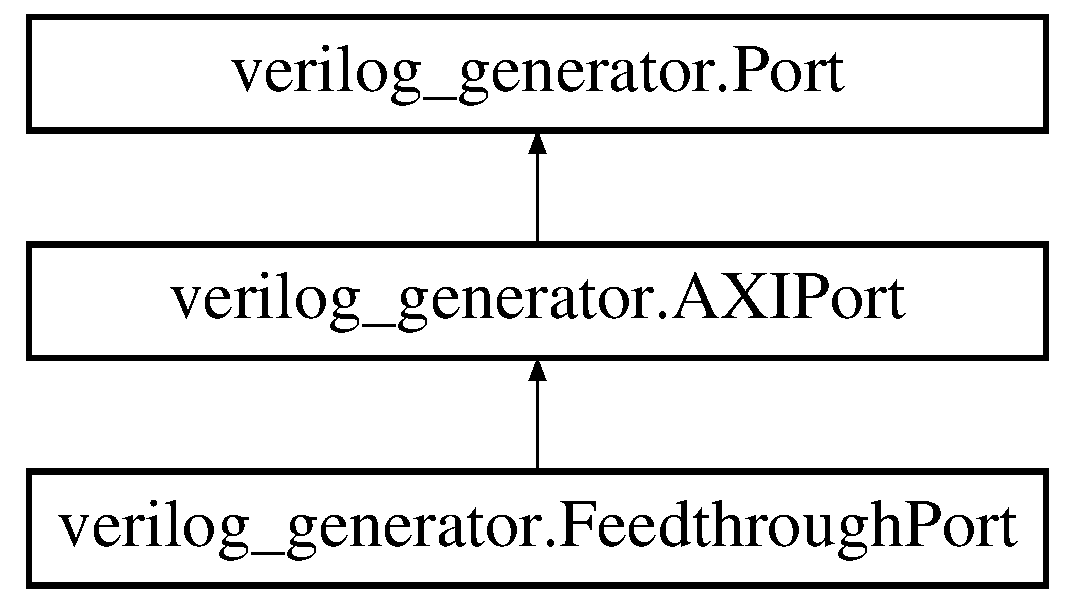
\includegraphics[height=3.000000cm]{classverilog__generator_1_1AXIPort}
\end{center}
\end{figure}
\subsection*{Public Member Functions}
\begin{DoxyCompactItemize}
\item 
def \hyperlink{classverilog__generator_1_1AXIPort_a361d2bda856fc56834185a84a380cda4}{\-\_\-\-\_\-init\-\_\-\-\_\-}
\item 
def \hyperlink{classverilog__generator_1_1AXIPort_af08a76ecfd4a6978c60888ef47f39309}{name}
\item 
def \hyperlink{classverilog__generator_1_1AXIPort_af08a76ecfd4a6978c60888ef47f39309}{name}
\item 
def \hyperlink{classverilog__generator_1_1AXIPort_ae3017dd2386c7e09cbf6b79a569bf471}{port\-\_\-name}
\end{DoxyCompactItemize}
\subsection*{Public Attributes}
\begin{DoxyCompactItemize}
\item 
\hyperlink{classverilog__generator_1_1AXIPort_a12216f6df7bee0b17bda71de5843b476}{bundle}
\end{DoxyCompactItemize}
\subsection*{Additional Inherited Members}


\subsection{Constructor \& Destructor Documentation}
\hypertarget{classverilog__generator_1_1AXIPort_a361d2bda856fc56834185a84a380cda4}{\index{verilog\-\_\-generator\-::\-A\-X\-I\-Port@{verilog\-\_\-generator\-::\-A\-X\-I\-Port}!\-\_\-\-\_\-init\-\_\-\-\_\-@{\-\_\-\-\_\-init\-\_\-\-\_\-}}
\index{\-\_\-\-\_\-init\-\_\-\-\_\-@{\-\_\-\-\_\-init\-\_\-\-\_\-}!verilog_generator::AXIPort@{verilog\-\_\-generator\-::\-A\-X\-I\-Port}}
\subsubsection[{\-\_\-\-\_\-init\-\_\-\-\_\-}]{\setlength{\rightskip}{0pt plus 5cm}def verilog\-\_\-generator.\-A\-X\-I\-Port.\-\_\-\-\_\-init\-\_\-\-\_\- (
\begin{DoxyParamCaption}
\item[{}]{self, }
\item[{}]{args, }
\item[{}]{kwargs}
\end{DoxyParamCaption}
)}}\label{classverilog__generator_1_1AXIPort_a361d2bda856fc56834185a84a380cda4}


\subsection{Member Function Documentation}
\hypertarget{classverilog__generator_1_1AXIPort_af08a76ecfd4a6978c60888ef47f39309}{\index{verilog\-\_\-generator\-::\-A\-X\-I\-Port@{verilog\-\_\-generator\-::\-A\-X\-I\-Port}!name@{name}}
\index{name@{name}!verilog_generator::AXIPort@{verilog\-\_\-generator\-::\-A\-X\-I\-Port}}
\subsubsection[{name}]{\setlength{\rightskip}{0pt plus 5cm}def verilog\-\_\-generator.\-A\-X\-I\-Port.\-name (
\begin{DoxyParamCaption}
\item[{}]{self, }
\item[{}]{str}
\end{DoxyParamCaption}
)}}\label{classverilog__generator_1_1AXIPort_af08a76ecfd4a6978c60888ef47f39309}
\hypertarget{classverilog__generator_1_1AXIPort_af08a76ecfd4a6978c60888ef47f39309}{\index{verilog\-\_\-generator\-::\-A\-X\-I\-Port@{verilog\-\_\-generator\-::\-A\-X\-I\-Port}!name@{name}}
\index{name@{name}!verilog_generator::AXIPort@{verilog\-\_\-generator\-::\-A\-X\-I\-Port}}
\subsubsection[{name}]{\setlength{\rightskip}{0pt plus 5cm}def verilog\-\_\-generator.\-A\-X\-I\-Port.\-name (
\begin{DoxyParamCaption}
\item[{}]{self, }
\item[{}]{n, }
\item[{}]{None}
\end{DoxyParamCaption}
)}}\label{classverilog__generator_1_1AXIPort_af08a76ecfd4a6978c60888ef47f39309}
\hypertarget{classverilog__generator_1_1AXIPort_ae3017dd2386c7e09cbf6b79a569bf471}{\index{verilog\-\_\-generator\-::\-A\-X\-I\-Port@{verilog\-\_\-generator\-::\-A\-X\-I\-Port}!port\-\_\-name@{port\-\_\-name}}
\index{port\-\_\-name@{port\-\_\-name}!verilog_generator::AXIPort@{verilog\-\_\-generator\-::\-A\-X\-I\-Port}}
\subsubsection[{port\-\_\-name}]{\setlength{\rightskip}{0pt plus 5cm}def verilog\-\_\-generator.\-A\-X\-I\-Port.\-port\-\_\-name (
\begin{DoxyParamCaption}
\item[{}]{self, }
\item[{}]{str}
\end{DoxyParamCaption}
)}}\label{classverilog__generator_1_1AXIPort_ae3017dd2386c7e09cbf6b79a569bf471}


\subsection{Member Data Documentation}
\hypertarget{classverilog__generator_1_1AXIPort_a12216f6df7bee0b17bda71de5843b476}{\index{verilog\-\_\-generator\-::\-A\-X\-I\-Port@{verilog\-\_\-generator\-::\-A\-X\-I\-Port}!bundle@{bundle}}
\index{bundle@{bundle}!verilog_generator::AXIPort@{verilog\-\_\-generator\-::\-A\-X\-I\-Port}}
\subsubsection[{bundle}]{\setlength{\rightskip}{0pt plus 5cm}verilog\-\_\-generator.\-A\-X\-I\-Port.\-bundle}}\label{classverilog__generator_1_1AXIPort_a12216f6df7bee0b17bda71de5843b476}


The documentation for this class was generated from the following file\-:\begin{DoxyCompactItemize}
\item 
\hyperlink{verilog__generator_8py}{verilog\-\_\-generator.\-py}\end{DoxyCompactItemize}

\hypertarget{classverilog__generator_1_1ClockResetPort}{\section{verilog\-\_\-generator.\-Clock\-Reset\-Port Class Reference}
\label{classverilog__generator_1_1ClockResetPort}\index{verilog\-\_\-generator.\-Clock\-Reset\-Port@{verilog\-\_\-generator.\-Clock\-Reset\-Port}}
}
Inheritance diagram for verilog\-\_\-generator.\-Clock\-Reset\-Port\-:\begin{figure}[H]
\begin{center}
\leavevmode
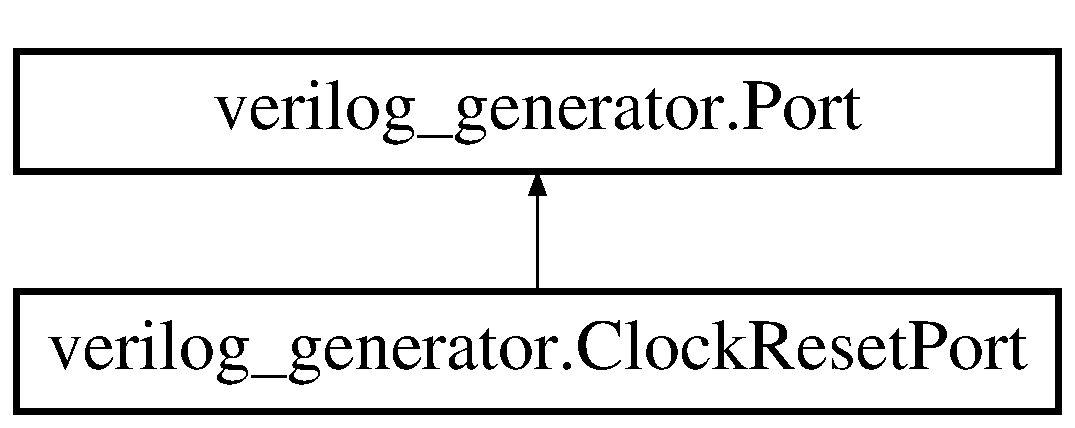
\includegraphics[height=2.000000cm]{classverilog__generator_1_1ClockResetPort}
\end{center}
\end{figure}
\subsection*{Public Member Functions}
\begin{DoxyCompactItemize}
\item 
def \hyperlink{classverilog__generator_1_1ClockResetPort_ad17226c115ee1037bebf401898c8f4b8}{\-\_\-\-\_\-init\-\_\-\-\_\-}
\item 
def \hyperlink{classverilog__generator_1_1ClockResetPort_a9d0fdc46490486651eeb7ee5fb3329a1}{\-\_\-\-\_\-invert\-\_\-\-\_\-}
\item 
def \hyperlink{classverilog__generator_1_1ClockResetPort_a3d1d318dec4561a26841184f897d08b3}{port\-\_\-name}
\item 
def \hyperlink{classverilog__generator_1_1ClockResetPort_a3a7abd08703934df6bec96f8e8690142}{wire\-\_\-name}
\end{DoxyCompactItemize}
\subsection*{Additional Inherited Members}


\subsection{Detailed Description}
\begin{DoxyVerb}clock reset port is a special port that cannot negate
its direction, and is always input with width of 1
never a feedthrough port, no path
\end{DoxyVerb}
 

\subsection{Constructor \& Destructor Documentation}
\hypertarget{classverilog__generator_1_1ClockResetPort_ad17226c115ee1037bebf401898c8f4b8}{\index{verilog\-\_\-generator\-::\-Clock\-Reset\-Port@{verilog\-\_\-generator\-::\-Clock\-Reset\-Port}!\-\_\-\-\_\-init\-\_\-\-\_\-@{\-\_\-\-\_\-init\-\_\-\-\_\-}}
\index{\-\_\-\-\_\-init\-\_\-\-\_\-@{\-\_\-\-\_\-init\-\_\-\-\_\-}!verilog_generator::ClockResetPort@{verilog\-\_\-generator\-::\-Clock\-Reset\-Port}}
\subsubsection[{\-\_\-\-\_\-init\-\_\-\-\_\-}]{\setlength{\rightskip}{0pt plus 5cm}def verilog\-\_\-generator.\-Clock\-Reset\-Port.\-\_\-\-\_\-init\-\_\-\-\_\- (
\begin{DoxyParamCaption}
\item[{}]{self, }
\item[{}]{name}
\end{DoxyParamCaption}
)}}\label{classverilog__generator_1_1ClockResetPort_ad17226c115ee1037bebf401898c8f4b8}


\subsection{Member Function Documentation}
\hypertarget{classverilog__generator_1_1ClockResetPort_a9d0fdc46490486651eeb7ee5fb3329a1}{\index{verilog\-\_\-generator\-::\-Clock\-Reset\-Port@{verilog\-\_\-generator\-::\-Clock\-Reset\-Port}!\-\_\-\-\_\-invert\-\_\-\-\_\-@{\-\_\-\-\_\-invert\-\_\-\-\_\-}}
\index{\-\_\-\-\_\-invert\-\_\-\-\_\-@{\-\_\-\-\_\-invert\-\_\-\-\_\-}!verilog_generator::ClockResetPort@{verilog\-\_\-generator\-::\-Clock\-Reset\-Port}}
\subsubsection[{\-\_\-\-\_\-invert\-\_\-\-\_\-}]{\setlength{\rightskip}{0pt plus 5cm}def verilog\-\_\-generator.\-Clock\-Reset\-Port.\-\_\-\-\_\-invert\-\_\-\-\_\- (
\begin{DoxyParamCaption}
\item[{}]{self, }
\item[{}]{Port}
\end{DoxyParamCaption}
)}}\label{classverilog__generator_1_1ClockResetPort_a9d0fdc46490486651eeb7ee5fb3329a1}
\hypertarget{classverilog__generator_1_1ClockResetPort_a3d1d318dec4561a26841184f897d08b3}{\index{verilog\-\_\-generator\-::\-Clock\-Reset\-Port@{verilog\-\_\-generator\-::\-Clock\-Reset\-Port}!port\-\_\-name@{port\-\_\-name}}
\index{port\-\_\-name@{port\-\_\-name}!verilog_generator::ClockResetPort@{verilog\-\_\-generator\-::\-Clock\-Reset\-Port}}
\subsubsection[{port\-\_\-name}]{\setlength{\rightskip}{0pt plus 5cm}def verilog\-\_\-generator.\-Clock\-Reset\-Port.\-port\-\_\-name (
\begin{DoxyParamCaption}
\item[{}]{self, }
\item[{}]{str}
\end{DoxyParamCaption}
)}}\label{classverilog__generator_1_1ClockResetPort_a3d1d318dec4561a26841184f897d08b3}
\begin{DoxyVerb}clk reset does not need to have src_dst prefix
\end{DoxyVerb}
 \hypertarget{classverilog__generator_1_1ClockResetPort_a3a7abd08703934df6bec96f8e8690142}{\index{verilog\-\_\-generator\-::\-Clock\-Reset\-Port@{verilog\-\_\-generator\-::\-Clock\-Reset\-Port}!wire\-\_\-name@{wire\-\_\-name}}
\index{wire\-\_\-name@{wire\-\_\-name}!verilog_generator::ClockResetPort@{verilog\-\_\-generator\-::\-Clock\-Reset\-Port}}
\subsubsection[{wire\-\_\-name}]{\setlength{\rightskip}{0pt plus 5cm}def verilog\-\_\-generator.\-Clock\-Reset\-Port.\-wire\-\_\-name (
\begin{DoxyParamCaption}
\item[{}]{self, }
\item[{}]{str}
\end{DoxyParamCaption}
)}}\label{classverilog__generator_1_1ClockResetPort_a3a7abd08703934df6bec96f8e8690142}


The documentation for this class was generated from the following file\-:\begin{DoxyCompactItemize}
\item 
\hyperlink{verilog__generator_8py}{verilog\-\_\-generator.\-py}\end{DoxyCompactItemize}

\hypertarget{classsrc_1_1codegen_1_1codegen}{\section{src.\-codegen.\-codegen Class Reference}
\label{classsrc_1_1codegen_1_1codegen}\index{src.\-codegen.\-codegen@{src.\-codegen.\-codegen}}
}
\subsection*{Public Member Functions}
\begin{DoxyCompactItemize}
\item 
def \hyperlink{classsrc_1_1codegen_1_1codegen_a398aadb5efcb770f3a620377176f30e8}{\-\_\-\-\_\-init\-\_\-\-\_\-}
\item 
def \hyperlink{classsrc_1_1codegen_1_1codegen_a8c0c108747245b54d7db81573b81dceb}{dbg\-\_\-store}
\item 
def \hyperlink{classsrc_1_1codegen_1_1codegen_a60ca6e690218d7156d86b764bbb610a4}{dbg}
\item 
def \hyperlink{classsrc_1_1codegen_1_1codegen_a44f570694e36b5ea23f568e01496623c}{get\-\_\-hash\-\_\-defval}
\item 
def \hyperlink{classsrc_1_1codegen_1_1codegen_a32c2b7a8fa27ff898939f71249f3226a}{split\-\_\-on\-\_\-word\-\_\-boundary}
\item 
def \hyperlink{classsrc_1_1codegen_1_1codegen_abdabc0d5fbdb726bcf0aa04efaf7e1b9}{find\-\_\-in\-\_\-files}
\item 
def \hyperlink{classsrc_1_1codegen_1_1codegen_ad1009199bc34ca1ebdee4724aaa4e9f5}{hash\-\_\-def\-\_\-getval}
\item 
def \hyperlink{classsrc_1_1codegen_1_1codegen_afee64e2ab5666640bdb2f9646b17ec06}{hash\-\_\-def\-\_\-proc}
\item 
def \hyperlink{classsrc_1_1codegen_1_1codegen_aed488c2ca235a59f579579f10e6ae427}{hash\-\_\-ifdef\-\_\-proc}
\item 
def \hyperlink{classsrc_1_1codegen_1_1codegen_a60aaf97546f41a1f135ef50cf1554df9}{load\-\_\-hash\-\_\-include\-\_\-file}
\item 
def \hyperlink{classsrc_1_1codegen_1_1codegen_a1407f81e5ffd9c6d084791bc865efad8}{generate\-\_\-code}
\item 
def \hyperlink{classsrc_1_1codegen_1_1codegen_af5b1063b6e2fc66994261e2a33cfeb14}{fsm}
\item 
def \hyperlink{classsrc_1_1codegen_1_1codegen_a53e8215ac19c4923e57f2a5dc40f127d}{pipe}
\item 
def \hyperlink{classsrc_1_1codegen_1_1codegen_acea965b006a0586d8da7aa4ab53081ea}{flop}
\end{DoxyCompactItemize}
\subsection*{Public Attributes}
\begin{DoxyCompactItemize}
\item 
\hyperlink{classsrc_1_1codegen_1_1codegen_a924b875eb5083c8e386a7c511062ec54}{in\-\_\-file}
\item 
\hyperlink{classsrc_1_1codegen_1_1codegen_a99a93980ce41f26c98d7310e896683e8}{remove\-\_\-code}
\item 
\hyperlink{classsrc_1_1codegen_1_1codegen_a52709f08304690031810bc906e79ee04}{incl\-\_\-dirs}
\item 
\hyperlink{classsrc_1_1codegen_1_1codegen_a0a7d1f62b91579d6cacc4051ab710f9d}{files}
\item 
\hyperlink{classsrc_1_1codegen_1_1codegen_a1dc7058a4be04c25dbeda35f53ad6561}{debug}
\item 
\hyperlink{classsrc_1_1codegen_1_1codegen_a7b9958156cd5e9db7a5065e37d8c2e3e}{debug\-\_\-file}
\item 
\hyperlink{classsrc_1_1codegen_1_1codegen_af63c5fcc7e7d1d62c3d7860151e68e4c}{gen\-\_\-dependencies}
\item 
\hyperlink{classsrc_1_1codegen_1_1codegen_a58d96416c95cad22a87488d65fb6fef5}{parsing\-\_\-format}
\item 
\hyperlink{classsrc_1_1codegen_1_1codegen_a2b49150564c96b7417c676c7e71f3ee3}{debug\-\_\-print}
\item 
\hyperlink{classsrc_1_1codegen_1_1codegen_a6566d2de6d4841695e4f1ef3eb89b8e9}{hash\-\_\-define\-\_\-vars}
\item 
\hyperlink{classsrc_1_1codegen_1_1codegen_a060c03d571c3d2aeb4cae7c50b1f23f9}{hash\-\_\-define\-\_\-files}
\item 
\hyperlink{classsrc_1_1codegen_1_1codegen_a8c1fbafee413be6472edfa3086744088}{hash\-\_\-defines}
\item 
\hyperlink{classsrc_1_1codegen_1_1codegen_a0d57c346d2836db9ede8bba7d2a94fdf}{hash\-\_\-ifdef\-\_\-en}
\begin{DoxyCompactList}\small\item\em Gathering Stub output overriding vals from verilog files that are commented. \end{DoxyCompactList}\item 
\hyperlink{classsrc_1_1codegen_1_1codegen_acc991347bbd3ec540567af9f2f45badd}{hash\-\_\-ifdef\-\_\-arr}
\item 
\hyperlink{classsrc_1_1codegen_1_1codegen_a235daa673c6d109632947f82e699b23d}{hash\-\_\-decisions}
\item 
\hyperlink{classsrc_1_1codegen_1_1codegen_a7d558f65ce1c06aac95ff81ccf6d7c56}{hash\-\_\-types}
\item 
\hyperlink{classsrc_1_1codegen_1_1codegen_aeb496fa242e02add6763b1231c8d0d6b}{hash\-\_\-served}
\item 
\hyperlink{classsrc_1_1codegen_1_1codegen_acd0bbf5623e10244e004795c4d6c9864}{hash\-\_\-curr\-\_\-decision}
\item 
\hyperlink{classsrc_1_1codegen_1_1codegen_ac52d0ff2519dcd3e385ec3f935dcef12}{hash\-\_\-curr\-\_\-type}
\item 
\hyperlink{classsrc_1_1codegen_1_1codegen_a4694bff348e2ec720f070f5a00a7627b}{hash\-\_\-curr\-\_\-served}
\item 
\hyperlink{classsrc_1_1codegen_1_1codegen_a8f9a4a6acf2e5f4fcc0043f0e336038c}{last\-\_\-hash\-\_\-loc}
\item 
\hyperlink{classsrc_1_1codegen_1_1codegen_aa67c1b409ff5dc21b0b29d4fd3d988a8}{line\-\_\-no}
\item 
\hyperlink{classsrc_1_1codegen_1_1codegen_a3e981982a203117a89f0216220ef35e2}{in\-\_\-lines}
\item 
\hyperlink{classsrc_1_1codegen_1_1codegen_a44287f529d387856ea12616f732da4a5}{clock}
\begin{DoxyCompactList}\small\item\em \&F\-S\-M Plugin \end{DoxyCompactList}\item 
\hyperlink{classsrc_1_1codegen_1_1codegen_ab571c5a0ed4af1f6549139c176f81ba8}{async\-\_\-reset}
\item 
\hyperlink{classsrc_1_1codegen_1_1codegen_a0dd09f1e941ca7d548ea6a62f4700b12}{sync\-\_\-reset}
\item 
\hyperlink{classsrc_1_1codegen_1_1codegen_ab41ce0ced866deb9f87c24ec402bb038}{reset\-\_\-type}
\item 
\hyperlink{classsrc_1_1codegen_1_1codegen_acbf0d11c53c3622ca9882109a9426f47}{stub\-\_\-override\-\_\-val}
\item 
\hyperlink{classsrc_1_1codegen_1_1codegen_aadf9a8ccf3c2cfbe223263585df2c595}{functions\-\_\-list}
\item 
\hyperlink{classsrc_1_1codegen_1_1codegen_a273a52ad4514be187aa19a8d2a680af1}{lines}
\item 
\hyperlink{classsrc_1_1codegen_1_1codegen_a2c0f2e58bab2bee51d4bd29101cdc68f}{debug\-\_\-info}
\item 
\hyperlink{classsrc_1_1codegen_1_1codegen_a255b1b73758f8a9f1e6a2fe555f9f6f8}{found\-\_\-error}
\begin{DoxyCompactList}\small\item\em Replace all the \#define variables \#\{{\itshape \} with values. }\end{DoxyCompactList}\item 
\hyperlink{classsrc_1_1codegen_1_1codegen_ab99ac25e057b9cc6007f411d7f7bb586}{header\-\_\-files}
\item 
\hyperlink{classsrc_1_1codegen_1_1codegen_ab37d0cfef8135e7c4be46e1592a8ca06}{dbg\-\_\-file}
\end{DoxyCompactItemize}


\subsection{Detailed Description}
\begin{DoxyVerb}Class to do the code generation part.
Parse #ifdef and work on only enabled code
Expand embedded python code output
Run plugin and generate code
\end{DoxyVerb}
 

\subsection{Constructor \& Destructor Documentation}
\hypertarget{classsrc_1_1codegen_1_1codegen_a398aadb5efcb770f3a620377176f30e8}{\index{src\-::codegen\-::codegen@{src\-::codegen\-::codegen}!\-\_\-\-\_\-init\-\_\-\-\_\-@{\-\_\-\-\_\-init\-\_\-\-\_\-}}
\index{\-\_\-\-\_\-init\-\_\-\-\_\-@{\-\_\-\-\_\-init\-\_\-\-\_\-}!src::codegen::codegen@{src\-::codegen\-::codegen}}
\subsubsection[{\-\_\-\-\_\-init\-\_\-\-\_\-}]{\setlength{\rightskip}{0pt plus 5cm}def src.\-codegen.\-codegen.\-\_\-\-\_\-init\-\_\-\-\_\- (
\begin{DoxyParamCaption}
\item[{}]{self, }
\item[{}]{in\-\_\-file, }
\item[{}]{rm\-\_\-code, }
\item[{}]{incl\-\_\-dirs, }
\item[{}]{files, }
\item[{}]{debug\-\_\-en, }
\item[{}]{debug\-\_\-file, }
\item[{}]{gen\-\_\-dependencies, }
\item[{}]{cmdline}
\end{DoxyParamCaption}
)}}\label{classsrc_1_1codegen_1_1codegen_a398aadb5efcb770f3a620377176f30e8}
\begin{DoxyVerb}Constructor
\end{DoxyVerb}
 

\subsection{Member Function Documentation}
\hypertarget{classsrc_1_1codegen_1_1codegen_a60ca6e690218d7156d86b764bbb610a4}{\index{src\-::codegen\-::codegen@{src\-::codegen\-::codegen}!dbg@{dbg}}
\index{dbg@{dbg}!src::codegen::codegen@{src\-::codegen\-::codegen}}
\subsubsection[{dbg}]{\setlength{\rightskip}{0pt plus 5cm}def src.\-codegen.\-codegen.\-dbg (
\begin{DoxyParamCaption}
\item[{}]{self, }
\item[{}]{dbg\-\_\-info}
\end{DoxyParamCaption}
)}}\label{classsrc_1_1codegen_1_1codegen_a60ca6e690218d7156d86b764bbb610a4}
\begin{DoxyVerb}Function to print a debug string in a debug dump file
\end{DoxyVerb}
 \hypertarget{classsrc_1_1codegen_1_1codegen_a8c0c108747245b54d7db81573b81dceb}{\index{src\-::codegen\-::codegen@{src\-::codegen\-::codegen}!dbg\-\_\-store@{dbg\-\_\-store}}
\index{dbg\-\_\-store@{dbg\-\_\-store}!src::codegen::codegen@{src\-::codegen\-::codegen}}
\subsubsection[{dbg\-\_\-store}]{\setlength{\rightskip}{0pt plus 5cm}def src.\-codegen.\-codegen.\-dbg\-\_\-store (
\begin{DoxyParamCaption}
\item[{}]{self, }
\item[{}]{dbg\-\_\-info}
\end{DoxyParamCaption}
)}}\label{classsrc_1_1codegen_1_1codegen_a8c0c108747245b54d7db81573b81dceb}
\begin{DoxyVerb}Function to print a debug string in a debug dump file
\end{DoxyVerb}
 \hypertarget{classsrc_1_1codegen_1_1codegen_abdabc0d5fbdb726bcf0aa04efaf7e1b9}{\index{src\-::codegen\-::codegen@{src\-::codegen\-::codegen}!find\-\_\-in\-\_\-files@{find\-\_\-in\-\_\-files}}
\index{find\-\_\-in\-\_\-files@{find\-\_\-in\-\_\-files}!src::codegen::codegen@{src\-::codegen\-::codegen}}
\subsubsection[{find\-\_\-in\-\_\-files}]{\setlength{\rightskip}{0pt plus 5cm}def src.\-codegen.\-codegen.\-find\-\_\-in\-\_\-files (
\begin{DoxyParamCaption}
\item[{}]{self, }
\item[{}]{filename}
\end{DoxyParamCaption}
)}}\label{classsrc_1_1codegen_1_1codegen_abdabc0d5fbdb726bcf0aa04efaf7e1b9}
\begin{DoxyVerb}Function to print a debug string in a debug dump file
\end{DoxyVerb}
 \hypertarget{classsrc_1_1codegen_1_1codegen_acea965b006a0586d8da7aa4ab53081ea}{\index{src\-::codegen\-::codegen@{src\-::codegen\-::codegen}!flop@{flop}}
\index{flop@{flop}!src::codegen::codegen@{src\-::codegen\-::codegen}}
\subsubsection[{flop}]{\setlength{\rightskip}{0pt plus 5cm}def src.\-codegen.\-codegen.\-flop (
\begin{DoxyParamCaption}
\item[{}]{self, }
\item[{}]{flop\-\_\-type, }
\item[{}]{flop\-\_\-string}
\end{DoxyParamCaption}
)}}\label{classsrc_1_1codegen_1_1codegen_acea965b006a0586d8da7aa4ab53081ea}
\begin{DoxyVerb}Flop code generation
\end{DoxyVerb}
 \hypertarget{classsrc_1_1codegen_1_1codegen_af5b1063b6e2fc66994261e2a33cfeb14}{\index{src\-::codegen\-::codegen@{src\-::codegen\-::codegen}!fsm@{fsm}}
\index{fsm@{fsm}!src::codegen::codegen@{src\-::codegen\-::codegen}}
\subsubsection[{fsm}]{\setlength{\rightskip}{0pt plus 5cm}def src.\-codegen.\-codegen.\-fsm (
\begin{DoxyParamCaption}
\item[{}]{self, }
\item[{}]{inp\-\_\-str}
\end{DoxyParamCaption}
)}}\label{classsrc_1_1codegen_1_1codegen_af5b1063b6e2fc66994261e2a33cfeb14}
\begin{DoxyVerb}FSM plugin code generation
\end{DoxyVerb}
 \hypertarget{classsrc_1_1codegen_1_1codegen_a1407f81e5ffd9c6d084791bc865efad8}{\index{src\-::codegen\-::codegen@{src\-::codegen\-::codegen}!generate\-\_\-code@{generate\-\_\-code}}
\index{generate\-\_\-code@{generate\-\_\-code}!src::codegen::codegen@{src\-::codegen\-::codegen}}
\subsubsection[{generate\-\_\-code}]{\setlength{\rightskip}{0pt plus 5cm}def src.\-codegen.\-codegen.\-generate\-\_\-code (
\begin{DoxyParamCaption}
\item[{}]{self, }
\item[{}]{module\-\_\-name}
\end{DoxyParamCaption}
)}}\label{classsrc_1_1codegen_1_1codegen_a1407f81e5ffd9c6d084791bc865efad8}
\begin{DoxyVerb}Main code generation function
\end{DoxyVerb}
 \hypertarget{classsrc_1_1codegen_1_1codegen_a44f570694e36b5ea23f568e01496623c}{\index{src\-::codegen\-::codegen@{src\-::codegen\-::codegen}!get\-\_\-hash\-\_\-defval@{get\-\_\-hash\-\_\-defval}}
\index{get\-\_\-hash\-\_\-defval@{get\-\_\-hash\-\_\-defval}!src::codegen::codegen@{src\-::codegen\-::codegen}}
\subsubsection[{get\-\_\-hash\-\_\-defval}]{\setlength{\rightskip}{0pt plus 5cm}def src.\-codegen.\-codegen.\-get\-\_\-hash\-\_\-defval (
\begin{DoxyParamCaption}
\item[{}]{self, }
\item[{}]{hash\-\_\-def}
\end{DoxyParamCaption}
)}}\label{classsrc_1_1codegen_1_1codegen_a44f570694e36b5ea23f568e01496623c}
\begin{DoxyVerb}Function to get the value of a #define. This can be called in a embedded
python script.
\end{DoxyVerb}
 \hypertarget{classsrc_1_1codegen_1_1codegen_ad1009199bc34ca1ebdee4724aaa4e9f5}{\index{src\-::codegen\-::codegen@{src\-::codegen\-::codegen}!hash\-\_\-def\-\_\-getval@{hash\-\_\-def\-\_\-getval}}
\index{hash\-\_\-def\-\_\-getval@{hash\-\_\-def\-\_\-getval}!src::codegen::codegen@{src\-::codegen\-::codegen}}
\subsubsection[{hash\-\_\-def\-\_\-getval}]{\setlength{\rightskip}{0pt plus 5cm}def src.\-codegen.\-codegen.\-hash\-\_\-def\-\_\-getval (
\begin{DoxyParamCaption}
\item[{}]{self, }
\item[{}]{hash\-\_\-def\-\_\-exp}
\end{DoxyParamCaption}
)}}\label{classsrc_1_1codegen_1_1codegen_ad1009199bc34ca1ebdee4724aaa4e9f5}
\begin{DoxyVerb}Function to calculate value for a #define and return its type
Type can be numerical, string
\end{DoxyVerb}
 \hypertarget{classsrc_1_1codegen_1_1codegen_afee64e2ab5666640bdb2f9646b17ec06}{\index{src\-::codegen\-::codegen@{src\-::codegen\-::codegen}!hash\-\_\-def\-\_\-proc@{hash\-\_\-def\-\_\-proc}}
\index{hash\-\_\-def\-\_\-proc@{hash\-\_\-def\-\_\-proc}!src::codegen::codegen@{src\-::codegen\-::codegen}}
\subsubsection[{hash\-\_\-def\-\_\-proc}]{\setlength{\rightskip}{0pt plus 5cm}def src.\-codegen.\-codegen.\-hash\-\_\-def\-\_\-proc (
\begin{DoxyParamCaption}
\item[{}]{self, }
\item[{}]{hash\-\_\-def\-\_\-in}
\end{DoxyParamCaption}
)}}\label{classsrc_1_1codegen_1_1codegen_afee64e2ab5666640bdb2f9646b17ec06}
\begin{DoxyVerb}Function parses the #define and updates the hash table with value and type
\end{DoxyVerb}
 \hypertarget{classsrc_1_1codegen_1_1codegen_aed488c2ca235a59f579579f10e6ae427}{\index{src\-::codegen\-::codegen@{src\-::codegen\-::codegen}!hash\-\_\-ifdef\-\_\-proc@{hash\-\_\-ifdef\-\_\-proc}}
\index{hash\-\_\-ifdef\-\_\-proc@{hash\-\_\-ifdef\-\_\-proc}!src::codegen::codegen@{src\-::codegen\-::codegen}}
\subsubsection[{hash\-\_\-ifdef\-\_\-proc}]{\setlength{\rightskip}{0pt plus 5cm}def src.\-codegen.\-codegen.\-hash\-\_\-ifdef\-\_\-proc (
\begin{DoxyParamCaption}
\item[{}]{self, }
\item[{}]{hash\-\_\-ifdef\-\_\-type, }
\item[{}]{hash\-\_\-ifdef\-\_\-str}
\end{DoxyParamCaption}
)}}\label{classsrc_1_1codegen_1_1codegen_aed488c2ca235a59f579579f10e6ae427}
\begin{DoxyVerb}Function to process #ifdef and it returns current ifdef status
to skip the code or parse it
\end{DoxyVerb}
 \hypertarget{classsrc_1_1codegen_1_1codegen_a60aaf97546f41a1f135ef50cf1554df9}{\index{src\-::codegen\-::codegen@{src\-::codegen\-::codegen}!load\-\_\-hash\-\_\-include\-\_\-file@{load\-\_\-hash\-\_\-include\-\_\-file}}
\index{load\-\_\-hash\-\_\-include\-\_\-file@{load\-\_\-hash\-\_\-include\-\_\-file}!src::codegen::codegen@{src\-::codegen\-::codegen}}
\subsubsection[{load\-\_\-hash\-\_\-include\-\_\-file}]{\setlength{\rightskip}{0pt plus 5cm}def src.\-codegen.\-codegen.\-load\-\_\-hash\-\_\-include\-\_\-file (
\begin{DoxyParamCaption}
\item[{}]{self, }
\item[{}]{hash\-\_\-inc\-\_\-file}
\end{DoxyParamCaption}
)}}\label{classsrc_1_1codegen_1_1codegen_a60aaf97546f41a1f135ef50cf1554df9}
\begin{DoxyVerb}Function to parse an #include file
\end{DoxyVerb}
 \hypertarget{classsrc_1_1codegen_1_1codegen_a53e8215ac19c4923e57f2a5dc40f127d}{\index{src\-::codegen\-::codegen@{src\-::codegen\-::codegen}!pipe@{pipe}}
\index{pipe@{pipe}!src::codegen::codegen@{src\-::codegen\-::codegen}}
\subsubsection[{pipe}]{\setlength{\rightskip}{0pt plus 5cm}def src.\-codegen.\-codegen.\-pipe (
\begin{DoxyParamCaption}
\item[{}]{self, }
\item[{}]{inp\-\_\-str}
\end{DoxyParamCaption}
)}}\label{classsrc_1_1codegen_1_1codegen_a53e8215ac19c4923e57f2a5dc40f127d}
\begin{DoxyVerb}Pipe plugin code generation
\end{DoxyVerb}
 \hypertarget{classsrc_1_1codegen_1_1codegen_a32c2b7a8fa27ff898939f71249f3226a}{\index{src\-::codegen\-::codegen@{src\-::codegen\-::codegen}!split\-\_\-on\-\_\-word\-\_\-boundary@{split\-\_\-on\-\_\-word\-\_\-boundary}}
\index{split\-\_\-on\-\_\-word\-\_\-boundary@{split\-\_\-on\-\_\-word\-\_\-boundary}!src::codegen::codegen@{src\-::codegen\-::codegen}}
\subsubsection[{split\-\_\-on\-\_\-word\-\_\-boundary}]{\setlength{\rightskip}{0pt plus 5cm}def src.\-codegen.\-codegen.\-split\-\_\-on\-\_\-word\-\_\-boundary (
\begin{DoxyParamCaption}
\item[{}]{self, }
\item[{}]{string\-\_\-in}
\end{DoxyParamCaption}
)}}\label{classsrc_1_1codegen_1_1codegen_a32c2b7a8fa27ff898939f71249f3226a}
\begin{DoxyVerb}Function to split a string on a word boundary and return as an array
\end{DoxyVerb}
 

\subsection{Member Data Documentation}
\hypertarget{classsrc_1_1codegen_1_1codegen_ab571c5a0ed4af1f6549139c176f81ba8}{\index{src\-::codegen\-::codegen@{src\-::codegen\-::codegen}!async\-\_\-reset@{async\-\_\-reset}}
\index{async\-\_\-reset@{async\-\_\-reset}!src::codegen::codegen@{src\-::codegen\-::codegen}}
\subsubsection[{async\-\_\-reset}]{\setlength{\rightskip}{0pt plus 5cm}src.\-codegen.\-codegen.\-async\-\_\-reset}}\label{classsrc_1_1codegen_1_1codegen_ab571c5a0ed4af1f6549139c176f81ba8}
\hypertarget{classsrc_1_1codegen_1_1codegen_a44287f529d387856ea12616f732da4a5}{\index{src\-::codegen\-::codegen@{src\-::codegen\-::codegen}!clock@{clock}}
\index{clock@{clock}!src::codegen::codegen@{src\-::codegen\-::codegen}}
\subsubsection[{clock}]{\setlength{\rightskip}{0pt plus 5cm}src.\-codegen.\-codegen.\-clock}}\label{classsrc_1_1codegen_1_1codegen_a44287f529d387856ea12616f732da4a5}


\&F\-S\-M Plugin 

\&fb\-\_\-enflop / \&fb\-\_\-enflop\-\_\-rs / \&fb\-\_\-enflop\-\_\-rst Plugins \&Pipe Plugin \&Mem\-Gen Plugin \&Hls\-Mem\-Gen Plugin \&E\-C\-C\-Mem\-Gen Plugin Calculation on Width and Depth for E\-C\-C for example\-: 128 X 320 -\/ 2(128 X 160) Depth remain same -\/ 128 320 -\/ 2$^\wedge$(r-\/1) $>$= r+w \&Clock\-Gen Plugin Dump out line by line keeping U\-S\-E\-R's indentation \&Sync\-Gen Plugin \&Sync\-Gen(\char`\"{}$<$\-C\-L\-K$>$\char`\"{}, \char`\"{}$<$\-D\-A\-T\-A\-I\-N$>$\char`\"{}, \char`\"{}$<$\-D\-A\-T\-A\-O\-U\-T\char`\"{}, \char`\"{}$<$\-T\-E\-S\-T\-\_\-\-E\-N\-A\-B\-L\-E$>$\char`\"{}); $<$\-T\-E\-S\-T\-\_\-\-E\-N\-A\-B\-L\-E$>$ is optional and connect test\-\_\-enable \&Clock\-Reset\-Gen Plugin instantiates clock and reset syncronizer from free running clock and power on reset. \&Clock\-Reset\-Gen($<$source\-\_\-clk$>$, $<$reset\-\_\-in$>$, \char`\"{}$<$outclk\-\_\-prefix$>$\char`\"{}) outclk\-\_\-prefix can be one or more separated by , \&Posedge, \&Negedge, \&Clock, \&Sync\-Reset and \&Asyncreset \hypertarget{classsrc_1_1codegen_1_1codegen_ab37d0cfef8135e7c4be46e1592a8ca06}{\index{src\-::codegen\-::codegen@{src\-::codegen\-::codegen}!dbg\-\_\-file@{dbg\-\_\-file}}
\index{dbg\-\_\-file@{dbg\-\_\-file}!src::codegen::codegen@{src\-::codegen\-::codegen}}
\subsubsection[{dbg\-\_\-file}]{\setlength{\rightskip}{0pt plus 5cm}src.\-codegen.\-codegen.\-dbg\-\_\-file}}\label{classsrc_1_1codegen_1_1codegen_ab37d0cfef8135e7c4be46e1592a8ca06}
\hypertarget{classsrc_1_1codegen_1_1codegen_a1dc7058a4be04c25dbeda35f53ad6561}{\index{src\-::codegen\-::codegen@{src\-::codegen\-::codegen}!debug@{debug}}
\index{debug@{debug}!src::codegen::codegen@{src\-::codegen\-::codegen}}
\subsubsection[{debug}]{\setlength{\rightskip}{0pt plus 5cm}src.\-codegen.\-codegen.\-debug}}\label{classsrc_1_1codegen_1_1codegen_a1dc7058a4be04c25dbeda35f53ad6561}
\hypertarget{classsrc_1_1codegen_1_1codegen_a7b9958156cd5e9db7a5065e37d8c2e3e}{\index{src\-::codegen\-::codegen@{src\-::codegen\-::codegen}!debug\-\_\-file@{debug\-\_\-file}}
\index{debug\-\_\-file@{debug\-\_\-file}!src::codegen::codegen@{src\-::codegen\-::codegen}}
\subsubsection[{debug\-\_\-file}]{\setlength{\rightskip}{0pt plus 5cm}src.\-codegen.\-codegen.\-debug\-\_\-file}}\label{classsrc_1_1codegen_1_1codegen_a7b9958156cd5e9db7a5065e37d8c2e3e}
\hypertarget{classsrc_1_1codegen_1_1codegen_a2c0f2e58bab2bee51d4bd29101cdc68f}{\index{src\-::codegen\-::codegen@{src\-::codegen\-::codegen}!debug\-\_\-info@{debug\-\_\-info}}
\index{debug\-\_\-info@{debug\-\_\-info}!src::codegen::codegen@{src\-::codegen\-::codegen}}
\subsubsection[{debug\-\_\-info}]{\setlength{\rightskip}{0pt plus 5cm}src.\-codegen.\-codegen.\-debug\-\_\-info}}\label{classsrc_1_1codegen_1_1codegen_a2c0f2e58bab2bee51d4bd29101cdc68f}
\hypertarget{classsrc_1_1codegen_1_1codegen_a2b49150564c96b7417c676c7e71f3ee3}{\index{src\-::codegen\-::codegen@{src\-::codegen\-::codegen}!debug\-\_\-print@{debug\-\_\-print}}
\index{debug\-\_\-print@{debug\-\_\-print}!src::codegen::codegen@{src\-::codegen\-::codegen}}
\subsubsection[{debug\-\_\-print}]{\setlength{\rightskip}{0pt plus 5cm}src.\-codegen.\-codegen.\-debug\-\_\-print}}\label{classsrc_1_1codegen_1_1codegen_a2b49150564c96b7417c676c7e71f3ee3}
\hypertarget{classsrc_1_1codegen_1_1codegen_a0a7d1f62b91579d6cacc4051ab710f9d}{\index{src\-::codegen\-::codegen@{src\-::codegen\-::codegen}!files@{files}}
\index{files@{files}!src::codegen::codegen@{src\-::codegen\-::codegen}}
\subsubsection[{files}]{\setlength{\rightskip}{0pt plus 5cm}src.\-codegen.\-codegen.\-files}}\label{classsrc_1_1codegen_1_1codegen_a0a7d1f62b91579d6cacc4051ab710f9d}
\hypertarget{classsrc_1_1codegen_1_1codegen_a255b1b73758f8a9f1e6a2fe555f9f6f8}{\index{src\-::codegen\-::codegen@{src\-::codegen\-::codegen}!found\-\_\-error@{found\-\_\-error}}
\index{found\-\_\-error@{found\-\_\-error}!src::codegen::codegen@{src\-::codegen\-::codegen}}
\subsubsection[{found\-\_\-error}]{\setlength{\rightskip}{0pt plus 5cm}src.\-codegen.\-codegen.\-found\-\_\-error}}\label{classsrc_1_1codegen_1_1codegen_a255b1b73758f8a9f1e6a2fe555f9f6f8}


Replace all the \#define variables \#\{{\itshape \} with values. }

Gather the list of functions in the input file.

\#define processing \#undef processing \#include processing Embedded python script processing \hypertarget{classsrc_1_1codegen_1_1codegen_aadf9a8ccf3c2cfbe223263585df2c595}{\index{src\-::codegen\-::codegen@{src\-::codegen\-::codegen}!functions\-\_\-list@{functions\-\_\-list}}
\index{functions\-\_\-list@{functions\-\_\-list}!src::codegen::codegen@{src\-::codegen\-::codegen}}
\subsubsection[{functions\-\_\-list}]{\setlength{\rightskip}{0pt plus 5cm}src.\-codegen.\-codegen.\-functions\-\_\-list}}\label{classsrc_1_1codegen_1_1codegen_aadf9a8ccf3c2cfbe223263585df2c595}
\hypertarget{classsrc_1_1codegen_1_1codegen_af63c5fcc7e7d1d62c3d7860151e68e4c}{\index{src\-::codegen\-::codegen@{src\-::codegen\-::codegen}!gen\-\_\-dependencies@{gen\-\_\-dependencies}}
\index{gen\-\_\-dependencies@{gen\-\_\-dependencies}!src::codegen::codegen@{src\-::codegen\-::codegen}}
\subsubsection[{gen\-\_\-dependencies}]{\setlength{\rightskip}{0pt plus 5cm}src.\-codegen.\-codegen.\-gen\-\_\-dependencies}}\label{classsrc_1_1codegen_1_1codegen_af63c5fcc7e7d1d62c3d7860151e68e4c}
\hypertarget{classsrc_1_1codegen_1_1codegen_acd0bbf5623e10244e004795c4d6c9864}{\index{src\-::codegen\-::codegen@{src\-::codegen\-::codegen}!hash\-\_\-curr\-\_\-decision@{hash\-\_\-curr\-\_\-decision}}
\index{hash\-\_\-curr\-\_\-decision@{hash\-\_\-curr\-\_\-decision}!src::codegen::codegen@{src\-::codegen\-::codegen}}
\subsubsection[{hash\-\_\-curr\-\_\-decision}]{\setlength{\rightskip}{0pt plus 5cm}src.\-codegen.\-codegen.\-hash\-\_\-curr\-\_\-decision}}\label{classsrc_1_1codegen_1_1codegen_acd0bbf5623e10244e004795c4d6c9864}
\hypertarget{classsrc_1_1codegen_1_1codegen_a4694bff348e2ec720f070f5a00a7627b}{\index{src\-::codegen\-::codegen@{src\-::codegen\-::codegen}!hash\-\_\-curr\-\_\-served@{hash\-\_\-curr\-\_\-served}}
\index{hash\-\_\-curr\-\_\-served@{hash\-\_\-curr\-\_\-served}!src::codegen::codegen@{src\-::codegen\-::codegen}}
\subsubsection[{hash\-\_\-curr\-\_\-served}]{\setlength{\rightskip}{0pt plus 5cm}src.\-codegen.\-codegen.\-hash\-\_\-curr\-\_\-served}}\label{classsrc_1_1codegen_1_1codegen_a4694bff348e2ec720f070f5a00a7627b}
\hypertarget{classsrc_1_1codegen_1_1codegen_ac52d0ff2519dcd3e385ec3f935dcef12}{\index{src\-::codegen\-::codegen@{src\-::codegen\-::codegen}!hash\-\_\-curr\-\_\-type@{hash\-\_\-curr\-\_\-type}}
\index{hash\-\_\-curr\-\_\-type@{hash\-\_\-curr\-\_\-type}!src::codegen::codegen@{src\-::codegen\-::codegen}}
\subsubsection[{hash\-\_\-curr\-\_\-type}]{\setlength{\rightskip}{0pt plus 5cm}src.\-codegen.\-codegen.\-hash\-\_\-curr\-\_\-type}}\label{classsrc_1_1codegen_1_1codegen_ac52d0ff2519dcd3e385ec3f935dcef12}
\hypertarget{classsrc_1_1codegen_1_1codegen_a235daa673c6d109632947f82e699b23d}{\index{src\-::codegen\-::codegen@{src\-::codegen\-::codegen}!hash\-\_\-decisions@{hash\-\_\-decisions}}
\index{hash\-\_\-decisions@{hash\-\_\-decisions}!src::codegen::codegen@{src\-::codegen\-::codegen}}
\subsubsection[{hash\-\_\-decisions}]{\setlength{\rightskip}{0pt plus 5cm}src.\-codegen.\-codegen.\-hash\-\_\-decisions}}\label{classsrc_1_1codegen_1_1codegen_a235daa673c6d109632947f82e699b23d}
\hypertarget{classsrc_1_1codegen_1_1codegen_a060c03d571c3d2aeb4cae7c50b1f23f9}{\index{src\-::codegen\-::codegen@{src\-::codegen\-::codegen}!hash\-\_\-define\-\_\-files@{hash\-\_\-define\-\_\-files}}
\index{hash\-\_\-define\-\_\-files@{hash\-\_\-define\-\_\-files}!src::codegen::codegen@{src\-::codegen\-::codegen}}
\subsubsection[{hash\-\_\-define\-\_\-files}]{\setlength{\rightskip}{0pt plus 5cm}src.\-codegen.\-codegen.\-hash\-\_\-define\-\_\-files}}\label{classsrc_1_1codegen_1_1codegen_a060c03d571c3d2aeb4cae7c50b1f23f9}
\hypertarget{classsrc_1_1codegen_1_1codegen_a6566d2de6d4841695e4f1ef3eb89b8e9}{\index{src\-::codegen\-::codegen@{src\-::codegen\-::codegen}!hash\-\_\-define\-\_\-vars@{hash\-\_\-define\-\_\-vars}}
\index{hash\-\_\-define\-\_\-vars@{hash\-\_\-define\-\_\-vars}!src::codegen::codegen@{src\-::codegen\-::codegen}}
\subsubsection[{hash\-\_\-define\-\_\-vars}]{\setlength{\rightskip}{0pt plus 5cm}src.\-codegen.\-codegen.\-hash\-\_\-define\-\_\-vars}}\label{classsrc_1_1codegen_1_1codegen_a6566d2de6d4841695e4f1ef3eb89b8e9}
\hypertarget{classsrc_1_1codegen_1_1codegen_a8c1fbafee413be6472edfa3086744088}{\index{src\-::codegen\-::codegen@{src\-::codegen\-::codegen}!hash\-\_\-defines@{hash\-\_\-defines}}
\index{hash\-\_\-defines@{hash\-\_\-defines}!src::codegen::codegen@{src\-::codegen\-::codegen}}
\subsubsection[{hash\-\_\-defines}]{\setlength{\rightskip}{0pt plus 5cm}src.\-codegen.\-codegen.\-hash\-\_\-defines}}\label{classsrc_1_1codegen_1_1codegen_a8c1fbafee413be6472edfa3086744088}
\hypertarget{classsrc_1_1codegen_1_1codegen_acc991347bbd3ec540567af9f2f45badd}{\index{src\-::codegen\-::codegen@{src\-::codegen\-::codegen}!hash\-\_\-ifdef\-\_\-arr@{hash\-\_\-ifdef\-\_\-arr}}
\index{hash\-\_\-ifdef\-\_\-arr@{hash\-\_\-ifdef\-\_\-arr}!src::codegen::codegen@{src\-::codegen\-::codegen}}
\subsubsection[{hash\-\_\-ifdef\-\_\-arr}]{\setlength{\rightskip}{0pt plus 5cm}src.\-codegen.\-codegen.\-hash\-\_\-ifdef\-\_\-arr}}\label{classsrc_1_1codegen_1_1codegen_acc991347bbd3ec540567af9f2f45badd}
\hypertarget{classsrc_1_1codegen_1_1codegen_a0d57c346d2836db9ede8bba7d2a94fdf}{\index{src\-::codegen\-::codegen@{src\-::codegen\-::codegen}!hash\-\_\-ifdef\-\_\-en@{hash\-\_\-ifdef\-\_\-en}}
\index{hash\-\_\-ifdef\-\_\-en@{hash\-\_\-ifdef\-\_\-en}!src::codegen::codegen@{src\-::codegen\-::codegen}}
\subsubsection[{hash\-\_\-ifdef\-\_\-en}]{\setlength{\rightskip}{0pt plus 5cm}src.\-codegen.\-codegen.\-hash\-\_\-ifdef\-\_\-en}}\label{classsrc_1_1codegen_1_1codegen_a0d57c346d2836db9ede8bba7d2a94fdf}


Gathering Stub output overriding vals from verilog files that are commented. 

if the whole line is commented from the beginning \&Begin\-Skip and \&End\-Skip for codegen and parsing skip Gathering Stub output overriding vals Block comment check \hypertarget{classsrc_1_1codegen_1_1codegen_aeb496fa242e02add6763b1231c8d0d6b}{\index{src\-::codegen\-::codegen@{src\-::codegen\-::codegen}!hash\-\_\-served@{hash\-\_\-served}}
\index{hash\-\_\-served@{hash\-\_\-served}!src::codegen::codegen@{src\-::codegen\-::codegen}}
\subsubsection[{hash\-\_\-served}]{\setlength{\rightskip}{0pt plus 5cm}src.\-codegen.\-codegen.\-hash\-\_\-served}}\label{classsrc_1_1codegen_1_1codegen_aeb496fa242e02add6763b1231c8d0d6b}
\hypertarget{classsrc_1_1codegen_1_1codegen_a7d558f65ce1c06aac95ff81ccf6d7c56}{\index{src\-::codegen\-::codegen@{src\-::codegen\-::codegen}!hash\-\_\-types@{hash\-\_\-types}}
\index{hash\-\_\-types@{hash\-\_\-types}!src::codegen::codegen@{src\-::codegen\-::codegen}}
\subsubsection[{hash\-\_\-types}]{\setlength{\rightskip}{0pt plus 5cm}src.\-codegen.\-codegen.\-hash\-\_\-types}}\label{classsrc_1_1codegen_1_1codegen_a7d558f65ce1c06aac95ff81ccf6d7c56}
\hypertarget{classsrc_1_1codegen_1_1codegen_ab99ac25e057b9cc6007f411d7f7bb586}{\index{src\-::codegen\-::codegen@{src\-::codegen\-::codegen}!header\-\_\-files@{header\-\_\-files}}
\index{header\-\_\-files@{header\-\_\-files}!src::codegen::codegen@{src\-::codegen\-::codegen}}
\subsubsection[{header\-\_\-files}]{\setlength{\rightskip}{0pt plus 5cm}src.\-codegen.\-codegen.\-header\-\_\-files}}\label{classsrc_1_1codegen_1_1codegen_ab99ac25e057b9cc6007f411d7f7bb586}
\hypertarget{classsrc_1_1codegen_1_1codegen_a924b875eb5083c8e386a7c511062ec54}{\index{src\-::codegen\-::codegen@{src\-::codegen\-::codegen}!in\-\_\-file@{in\-\_\-file}}
\index{in\-\_\-file@{in\-\_\-file}!src::codegen::codegen@{src\-::codegen\-::codegen}}
\subsubsection[{in\-\_\-file}]{\setlength{\rightskip}{0pt plus 5cm}src.\-codegen.\-codegen.\-in\-\_\-file}}\label{classsrc_1_1codegen_1_1codegen_a924b875eb5083c8e386a7c511062ec54}
\hypertarget{classsrc_1_1codegen_1_1codegen_a3e981982a203117a89f0216220ef35e2}{\index{src\-::codegen\-::codegen@{src\-::codegen\-::codegen}!in\-\_\-lines@{in\-\_\-lines}}
\index{in\-\_\-lines@{in\-\_\-lines}!src::codegen::codegen@{src\-::codegen\-::codegen}}
\subsubsection[{in\-\_\-lines}]{\setlength{\rightskip}{0pt plus 5cm}src.\-codegen.\-codegen.\-in\-\_\-lines}}\label{classsrc_1_1codegen_1_1codegen_a3e981982a203117a89f0216220ef35e2}
\hypertarget{classsrc_1_1codegen_1_1codegen_a52709f08304690031810bc906e79ee04}{\index{src\-::codegen\-::codegen@{src\-::codegen\-::codegen}!incl\-\_\-dirs@{incl\-\_\-dirs}}
\index{incl\-\_\-dirs@{incl\-\_\-dirs}!src::codegen::codegen@{src\-::codegen\-::codegen}}
\subsubsection[{incl\-\_\-dirs}]{\setlength{\rightskip}{0pt plus 5cm}src.\-codegen.\-codegen.\-incl\-\_\-dirs}}\label{classsrc_1_1codegen_1_1codegen_a52709f08304690031810bc906e79ee04}
\hypertarget{classsrc_1_1codegen_1_1codegen_a8f9a4a6acf2e5f4fcc0043f0e336038c}{\index{src\-::codegen\-::codegen@{src\-::codegen\-::codegen}!last\-\_\-hash\-\_\-loc@{last\-\_\-hash\-\_\-loc}}
\index{last\-\_\-hash\-\_\-loc@{last\-\_\-hash\-\_\-loc}!src::codegen::codegen@{src\-::codegen\-::codegen}}
\subsubsection[{last\-\_\-hash\-\_\-loc}]{\setlength{\rightskip}{0pt plus 5cm}src.\-codegen.\-codegen.\-last\-\_\-hash\-\_\-loc}}\label{classsrc_1_1codegen_1_1codegen_a8f9a4a6acf2e5f4fcc0043f0e336038c}
\hypertarget{classsrc_1_1codegen_1_1codegen_aa67c1b409ff5dc21b0b29d4fd3d988a8}{\index{src\-::codegen\-::codegen@{src\-::codegen\-::codegen}!line\-\_\-no@{line\-\_\-no}}
\index{line\-\_\-no@{line\-\_\-no}!src::codegen::codegen@{src\-::codegen\-::codegen}}
\subsubsection[{line\-\_\-no}]{\setlength{\rightskip}{0pt plus 5cm}src.\-codegen.\-codegen.\-line\-\_\-no}}\label{classsrc_1_1codegen_1_1codegen_aa67c1b409ff5dc21b0b29d4fd3d988a8}
\hypertarget{classsrc_1_1codegen_1_1codegen_a273a52ad4514be187aa19a8d2a680af1}{\index{src\-::codegen\-::codegen@{src\-::codegen\-::codegen}!lines@{lines}}
\index{lines@{lines}!src::codegen::codegen@{src\-::codegen\-::codegen}}
\subsubsection[{lines}]{\setlength{\rightskip}{0pt plus 5cm}src.\-codegen.\-codegen.\-lines}}\label{classsrc_1_1codegen_1_1codegen_a273a52ad4514be187aa19a8d2a680af1}
\hypertarget{classsrc_1_1codegen_1_1codegen_a58d96416c95cad22a87488d65fb6fef5}{\index{src\-::codegen\-::codegen@{src\-::codegen\-::codegen}!parsing\-\_\-format@{parsing\-\_\-format}}
\index{parsing\-\_\-format@{parsing\-\_\-format}!src::codegen::codegen@{src\-::codegen\-::codegen}}
\subsubsection[{parsing\-\_\-format}]{\setlength{\rightskip}{0pt plus 5cm}src.\-codegen.\-codegen.\-parsing\-\_\-format}}\label{classsrc_1_1codegen_1_1codegen_a58d96416c95cad22a87488d65fb6fef5}
\hypertarget{classsrc_1_1codegen_1_1codegen_a99a93980ce41f26c98d7310e896683e8}{\index{src\-::codegen\-::codegen@{src\-::codegen\-::codegen}!remove\-\_\-code@{remove\-\_\-code}}
\index{remove\-\_\-code@{remove\-\_\-code}!src::codegen::codegen@{src\-::codegen\-::codegen}}
\subsubsection[{remove\-\_\-code}]{\setlength{\rightskip}{0pt plus 5cm}src.\-codegen.\-codegen.\-remove\-\_\-code}}\label{classsrc_1_1codegen_1_1codegen_a99a93980ce41f26c98d7310e896683e8}
\hypertarget{classsrc_1_1codegen_1_1codegen_ab41ce0ced866deb9f87c24ec402bb038}{\index{src\-::codegen\-::codegen@{src\-::codegen\-::codegen}!reset\-\_\-type@{reset\-\_\-type}}
\index{reset\-\_\-type@{reset\-\_\-type}!src::codegen::codegen@{src\-::codegen\-::codegen}}
\subsubsection[{reset\-\_\-type}]{\setlength{\rightskip}{0pt plus 5cm}src.\-codegen.\-codegen.\-reset\-\_\-type}}\label{classsrc_1_1codegen_1_1codegen_ab41ce0ced866deb9f87c24ec402bb038}
\hypertarget{classsrc_1_1codegen_1_1codegen_acbf0d11c53c3622ca9882109a9426f47}{\index{src\-::codegen\-::codegen@{src\-::codegen\-::codegen}!stub\-\_\-override\-\_\-val@{stub\-\_\-override\-\_\-val}}
\index{stub\-\_\-override\-\_\-val@{stub\-\_\-override\-\_\-val}!src::codegen::codegen@{src\-::codegen\-::codegen}}
\subsubsection[{stub\-\_\-override\-\_\-val}]{\setlength{\rightskip}{0pt plus 5cm}src.\-codegen.\-codegen.\-stub\-\_\-override\-\_\-val}}\label{classsrc_1_1codegen_1_1codegen_acbf0d11c53c3622ca9882109a9426f47}
\hypertarget{classsrc_1_1codegen_1_1codegen_a0dd09f1e941ca7d548ea6a62f4700b12}{\index{src\-::codegen\-::codegen@{src\-::codegen\-::codegen}!sync\-\_\-reset@{sync\-\_\-reset}}
\index{sync\-\_\-reset@{sync\-\_\-reset}!src::codegen::codegen@{src\-::codegen\-::codegen}}
\subsubsection[{sync\-\_\-reset}]{\setlength{\rightskip}{0pt plus 5cm}src.\-codegen.\-codegen.\-sync\-\_\-reset}}\label{classsrc_1_1codegen_1_1codegen_a0dd09f1e941ca7d548ea6a62f4700b12}


The documentation for this class was generated from the following file\-:\begin{DoxyCompactItemize}
\item 
src/\hyperlink{codegen_8py}{codegen.\-py}\end{DoxyCompactItemize}

\hypertarget{classfb__utils_1_1CustomOrderedDict}{\section{fb\-\_\-utils.\-Custom\-Ordered\-Dict Class Reference}
\label{classfb__utils_1_1CustomOrderedDict}\index{fb\-\_\-utils.\-Custom\-Ordered\-Dict@{fb\-\_\-utils.\-Custom\-Ordered\-Dict}}
}
Inheritance diagram for fb\-\_\-utils.\-Custom\-Ordered\-Dict\-:\begin{figure}[H]
\begin{center}
\leavevmode
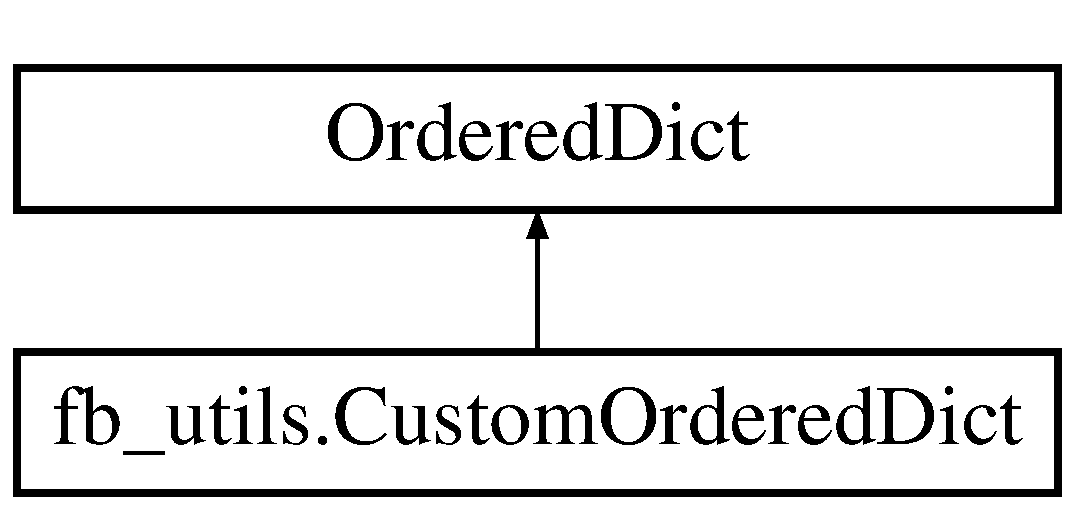
\includegraphics[height=2.000000cm]{classfb__utils_1_1CustomOrderedDict}
\end{center}
\end{figure}
\subsection*{Public Member Functions}
\begin{DoxyCompactItemize}
\item 
def \hyperlink{classfb__utils_1_1CustomOrderedDict_a198a41b0e78b5b3601747d6a463842cc}{\-\_\-\-\_\-getattr\-\_\-\-\_\-}
\item 
def \hyperlink{classfb__utils_1_1CustomOrderedDict_af91ffee0e17db9870195943378bb5418}{\-\_\-\-\_\-setattr\-\_\-\-\_\-}
\item 
def \hyperlink{classfb__utils_1_1CustomOrderedDict_a10a2c8eaad27d604efcab62d8a21f4b0}{\-\_\-\-\_\-delattr\-\_\-\-\_\-}
\end{DoxyCompactItemize}


\subsection{Detailed Description}
\begin{DoxyVerb}    a custom OrderedDict class that supports object-like dot notation
    perserving the ordering information in OrderedDict objects
\end{DoxyVerb}
 

\subsection{Member Function Documentation}
\hypertarget{classfb__utils_1_1CustomOrderedDict_a10a2c8eaad27d604efcab62d8a21f4b0}{\index{fb\-\_\-utils\-::\-Custom\-Ordered\-Dict@{fb\-\_\-utils\-::\-Custom\-Ordered\-Dict}!\-\_\-\-\_\-delattr\-\_\-\-\_\-@{\-\_\-\-\_\-delattr\-\_\-\-\_\-}}
\index{\-\_\-\-\_\-delattr\-\_\-\-\_\-@{\-\_\-\-\_\-delattr\-\_\-\-\_\-}!fb_utils::CustomOrderedDict@{fb\-\_\-utils\-::\-Custom\-Ordered\-Dict}}
\subsubsection[{\-\_\-\-\_\-delattr\-\_\-\-\_\-}]{\setlength{\rightskip}{0pt plus 5cm}def fb\-\_\-utils.\-Custom\-Ordered\-Dict.\-\_\-\-\_\-delattr\-\_\-\-\_\- (
\begin{DoxyParamCaption}
\item[{}]{self, }
\item[{}]{k}
\end{DoxyParamCaption}
)}}\label{classfb__utils_1_1CustomOrderedDict_a10a2c8eaad27d604efcab62d8a21f4b0}
\hypertarget{classfb__utils_1_1CustomOrderedDict_a198a41b0e78b5b3601747d6a463842cc}{\index{fb\-\_\-utils\-::\-Custom\-Ordered\-Dict@{fb\-\_\-utils\-::\-Custom\-Ordered\-Dict}!\-\_\-\-\_\-getattr\-\_\-\-\_\-@{\-\_\-\-\_\-getattr\-\_\-\-\_\-}}
\index{\-\_\-\-\_\-getattr\-\_\-\-\_\-@{\-\_\-\-\_\-getattr\-\_\-\-\_\-}!fb_utils::CustomOrderedDict@{fb\-\_\-utils\-::\-Custom\-Ordered\-Dict}}
\subsubsection[{\-\_\-\-\_\-getattr\-\_\-\-\_\-}]{\setlength{\rightskip}{0pt plus 5cm}def fb\-\_\-utils.\-Custom\-Ordered\-Dict.\-\_\-\-\_\-getattr\-\_\-\-\_\- (
\begin{DoxyParamCaption}
\item[{}]{self, }
\item[{}]{k}
\end{DoxyParamCaption}
)}}\label{classfb__utils_1_1CustomOrderedDict_a198a41b0e78b5b3601747d6a463842cc}
\hypertarget{classfb__utils_1_1CustomOrderedDict_af91ffee0e17db9870195943378bb5418}{\index{fb\-\_\-utils\-::\-Custom\-Ordered\-Dict@{fb\-\_\-utils\-::\-Custom\-Ordered\-Dict}!\-\_\-\-\_\-setattr\-\_\-\-\_\-@{\-\_\-\-\_\-setattr\-\_\-\-\_\-}}
\index{\-\_\-\-\_\-setattr\-\_\-\-\_\-@{\-\_\-\-\_\-setattr\-\_\-\-\_\-}!fb_utils::CustomOrderedDict@{fb\-\_\-utils\-::\-Custom\-Ordered\-Dict}}
\subsubsection[{\-\_\-\-\_\-setattr\-\_\-\-\_\-}]{\setlength{\rightskip}{0pt plus 5cm}def fb\-\_\-utils.\-Custom\-Ordered\-Dict.\-\_\-\-\_\-setattr\-\_\-\-\_\- (
\begin{DoxyParamCaption}
\item[{}]{self, }
\item[{}]{k, }
\item[{}]{v}
\end{DoxyParamCaption}
)}}\label{classfb__utils_1_1CustomOrderedDict_af91ffee0e17db9870195943378bb5418}


The documentation for this class was generated from the following file\-:\begin{DoxyCompactItemize}
\item 
\hyperlink{fb__utils_8py}{fb\-\_\-utils.\-py}\end{DoxyCompactItemize}

\hypertarget{classsrc_1_1fb__utils_1_1CustomOrderedDict}{\section{src.\-fb\-\_\-utils.\-Custom\-Ordered\-Dict Class Reference}
\label{classsrc_1_1fb__utils_1_1CustomOrderedDict}\index{src.\-fb\-\_\-utils.\-Custom\-Ordered\-Dict@{src.\-fb\-\_\-utils.\-Custom\-Ordered\-Dict}}
}
Inheritance diagram for src.\-fb\-\_\-utils.\-Custom\-Ordered\-Dict\-:\begin{figure}[H]
\begin{center}
\leavevmode
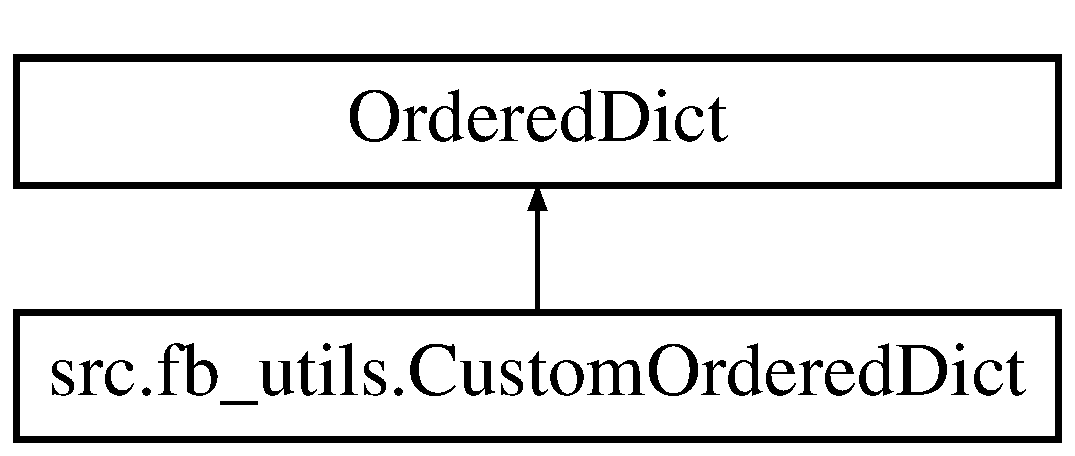
\includegraphics[height=2.000000cm]{classsrc_1_1fb__utils_1_1CustomOrderedDict}
\end{center}
\end{figure}
\subsection*{Public Member Functions}
\begin{DoxyCompactItemize}
\item 
def \hyperlink{classsrc_1_1fb__utils_1_1CustomOrderedDict_a90bf7568abbbac635c05e873d19ffe1c}{\-\_\-\-\_\-getattr\-\_\-\-\_\-}
\item 
def \hyperlink{classsrc_1_1fb__utils_1_1CustomOrderedDict_ac3246f459fdeadfbafe71d12a57f3046}{\-\_\-\-\_\-setattr\-\_\-\-\_\-}
\item 
def \hyperlink{classsrc_1_1fb__utils_1_1CustomOrderedDict_af9ab225f6b826341ea3df338127da156}{\-\_\-\-\_\-delattr\-\_\-\-\_\-}
\end{DoxyCompactItemize}


\subsection{Detailed Description}
\begin{DoxyVerb}    a custom OrderedDict class that supports object-like dot notation
    perserving the ordering information in OrderedDict objects
\end{DoxyVerb}
 

\subsection{Member Function Documentation}
\hypertarget{classsrc_1_1fb__utils_1_1CustomOrderedDict_af9ab225f6b826341ea3df338127da156}{\index{src\-::fb\-\_\-utils\-::\-Custom\-Ordered\-Dict@{src\-::fb\-\_\-utils\-::\-Custom\-Ordered\-Dict}!\-\_\-\-\_\-delattr\-\_\-\-\_\-@{\-\_\-\-\_\-delattr\-\_\-\-\_\-}}
\index{\-\_\-\-\_\-delattr\-\_\-\-\_\-@{\-\_\-\-\_\-delattr\-\_\-\-\_\-}!src::fb_utils::CustomOrderedDict@{src\-::fb\-\_\-utils\-::\-Custom\-Ordered\-Dict}}
\subsubsection[{\-\_\-\-\_\-delattr\-\_\-\-\_\-}]{\setlength{\rightskip}{0pt plus 5cm}def src.\-fb\-\_\-utils.\-Custom\-Ordered\-Dict.\-\_\-\-\_\-delattr\-\_\-\-\_\- (
\begin{DoxyParamCaption}
\item[{}]{self, }
\item[{}]{k}
\end{DoxyParamCaption}
)}}\label{classsrc_1_1fb__utils_1_1CustomOrderedDict_af9ab225f6b826341ea3df338127da156}
\hypertarget{classsrc_1_1fb__utils_1_1CustomOrderedDict_a90bf7568abbbac635c05e873d19ffe1c}{\index{src\-::fb\-\_\-utils\-::\-Custom\-Ordered\-Dict@{src\-::fb\-\_\-utils\-::\-Custom\-Ordered\-Dict}!\-\_\-\-\_\-getattr\-\_\-\-\_\-@{\-\_\-\-\_\-getattr\-\_\-\-\_\-}}
\index{\-\_\-\-\_\-getattr\-\_\-\-\_\-@{\-\_\-\-\_\-getattr\-\_\-\-\_\-}!src::fb_utils::CustomOrderedDict@{src\-::fb\-\_\-utils\-::\-Custom\-Ordered\-Dict}}
\subsubsection[{\-\_\-\-\_\-getattr\-\_\-\-\_\-}]{\setlength{\rightskip}{0pt plus 5cm}def src.\-fb\-\_\-utils.\-Custom\-Ordered\-Dict.\-\_\-\-\_\-getattr\-\_\-\-\_\- (
\begin{DoxyParamCaption}
\item[{}]{self, }
\item[{}]{k}
\end{DoxyParamCaption}
)}}\label{classsrc_1_1fb__utils_1_1CustomOrderedDict_a90bf7568abbbac635c05e873d19ffe1c}
\hypertarget{classsrc_1_1fb__utils_1_1CustomOrderedDict_ac3246f459fdeadfbafe71d12a57f3046}{\index{src\-::fb\-\_\-utils\-::\-Custom\-Ordered\-Dict@{src\-::fb\-\_\-utils\-::\-Custom\-Ordered\-Dict}!\-\_\-\-\_\-setattr\-\_\-\-\_\-@{\-\_\-\-\_\-setattr\-\_\-\-\_\-}}
\index{\-\_\-\-\_\-setattr\-\_\-\-\_\-@{\-\_\-\-\_\-setattr\-\_\-\-\_\-}!src::fb_utils::CustomOrderedDict@{src\-::fb\-\_\-utils\-::\-Custom\-Ordered\-Dict}}
\subsubsection[{\-\_\-\-\_\-setattr\-\_\-\-\_\-}]{\setlength{\rightskip}{0pt plus 5cm}def src.\-fb\-\_\-utils.\-Custom\-Ordered\-Dict.\-\_\-\-\_\-setattr\-\_\-\-\_\- (
\begin{DoxyParamCaption}
\item[{}]{self, }
\item[{}]{k, }
\item[{}]{v}
\end{DoxyParamCaption}
)}}\label{classsrc_1_1fb__utils_1_1CustomOrderedDict_ac3246f459fdeadfbafe71d12a57f3046}


The documentation for this class was generated from the following file\-:\begin{DoxyCompactItemize}
\item 
src/\hyperlink{src_2fb__utils_8py}{fb\-\_\-utils.\-py}\end{DoxyCompactItemize}

\hypertarget{classverilog__generator_1_1FeedthroughPort}{\section{verilog\-\_\-generator.\-Feedthrough\-Port Class Reference}
\label{classverilog__generator_1_1FeedthroughPort}\index{verilog\-\_\-generator.\-Feedthrough\-Port@{verilog\-\_\-generator.\-Feedthrough\-Port}}
}
Inheritance diagram for verilog\-\_\-generator.\-Feedthrough\-Port\-:\begin{figure}[H]
\begin{center}
\leavevmode
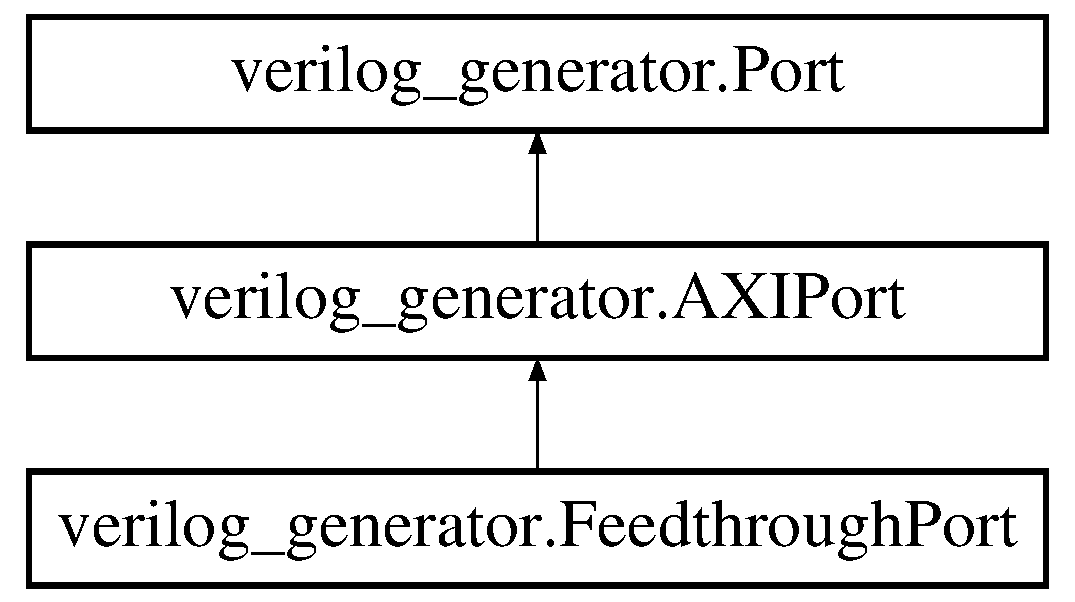
\includegraphics[height=3.000000cm]{classverilog__generator_1_1FeedthroughPort}
\end{center}
\end{figure}
\subsection*{Public Member Functions}
\begin{DoxyCompactItemize}
\item 
def \hyperlink{classverilog__generator_1_1FeedthroughPort_a7cf6834ae2da6dc67e70627eef8a7ed7}{\-\_\-\-\_\-init\-\_\-\-\_\-}
\item 
def \hyperlink{classverilog__generator_1_1FeedthroughPort_aaeaf2973a00aaf3d06525b2e9a508197}{port\-\_\-name}
\item 
def \hyperlink{classverilog__generator_1_1FeedthroughPort_af97681b3a72f75e91b9c4f25ad185509}{wire\-\_\-name}
\end{DoxyCompactItemize}
\subsection*{Public Attributes}
\begin{DoxyCompactItemize}
\item 
\hyperlink{classverilog__generator_1_1FeedthroughPort_acbb2b180844c87406724b2cf8f26de8d}{dir}
\end{DoxyCompactItemize}
\subsection*{Additional Inherited Members}


\subsection{Detailed Description}
\begin{DoxyVerb}ready port is a special port that always has the opposite direction
of other signals in an interface. but it's naming is still as if
has the same direction
\end{DoxyVerb}
 

\subsection{Constructor \& Destructor Documentation}
\hypertarget{classverilog__generator_1_1FeedthroughPort_a7cf6834ae2da6dc67e70627eef8a7ed7}{\index{verilog\-\_\-generator\-::\-Feedthrough\-Port@{verilog\-\_\-generator\-::\-Feedthrough\-Port}!\-\_\-\-\_\-init\-\_\-\-\_\-@{\-\_\-\-\_\-init\-\_\-\-\_\-}}
\index{\-\_\-\-\_\-init\-\_\-\-\_\-@{\-\_\-\-\_\-init\-\_\-\-\_\-}!verilog_generator::FeedthroughPort@{verilog\-\_\-generator\-::\-Feedthrough\-Port}}
\subsubsection[{\-\_\-\-\_\-init\-\_\-\-\_\-}]{\setlength{\rightskip}{0pt plus 5cm}def verilog\-\_\-generator.\-Feedthrough\-Port.\-\_\-\-\_\-init\-\_\-\-\_\- (
\begin{DoxyParamCaption}
\item[{}]{self, }
\item[{}]{args, }
\item[{}]{kwargs, }
\item[{}]{None}
\end{DoxyParamCaption}
)}}\label{classverilog__generator_1_1FeedthroughPort_a7cf6834ae2da6dc67e70627eef8a7ed7}


\subsection{Member Function Documentation}
\hypertarget{classverilog__generator_1_1FeedthroughPort_aaeaf2973a00aaf3d06525b2e9a508197}{\index{verilog\-\_\-generator\-::\-Feedthrough\-Port@{verilog\-\_\-generator\-::\-Feedthrough\-Port}!port\-\_\-name@{port\-\_\-name}}
\index{port\-\_\-name@{port\-\_\-name}!verilog_generator::FeedthroughPort@{verilog\-\_\-generator\-::\-Feedthrough\-Port}}
\subsubsection[{port\-\_\-name}]{\setlength{\rightskip}{0pt plus 5cm}def verilog\-\_\-generator.\-Feedthrough\-Port.\-port\-\_\-name (
\begin{DoxyParamCaption}
\item[{}]{self, }
\item[{}]{str}
\end{DoxyParamCaption}
)}}\label{classverilog__generator_1_1FeedthroughPort_aaeaf2973a00aaf3d06525b2e9a508197}
\begin{DoxyVerb}feedthrough ports name is
physrc_phydst_fti/o_src_dst_name
\end{DoxyVerb}
 \hypertarget{classverilog__generator_1_1FeedthroughPort_af97681b3a72f75e91b9c4f25ad185509}{\index{verilog\-\_\-generator\-::\-Feedthrough\-Port@{verilog\-\_\-generator\-::\-Feedthrough\-Port}!wire\-\_\-name@{wire\-\_\-name}}
\index{wire\-\_\-name@{wire\-\_\-name}!verilog_generator::FeedthroughPort@{verilog\-\_\-generator\-::\-Feedthrough\-Port}}
\subsubsection[{wire\-\_\-name}]{\setlength{\rightskip}{0pt plus 5cm}def verilog\-\_\-generator.\-Feedthrough\-Port.\-wire\-\_\-name (
\begin{DoxyParamCaption}
\item[{}]{self, }
\item[{}]{str}
\end{DoxyParamCaption}
)}}\label{classverilog__generator_1_1FeedthroughPort_af97681b3a72f75e91b9c4f25ad185509}
\begin{DoxyVerb}feedthrough ports name is
physrc_phydst_fti/o_src_dst_name
\end{DoxyVerb}
 

\subsection{Member Data Documentation}
\hypertarget{classverilog__generator_1_1FeedthroughPort_acbb2b180844c87406724b2cf8f26de8d}{\index{verilog\-\_\-generator\-::\-Feedthrough\-Port@{verilog\-\_\-generator\-::\-Feedthrough\-Port}!dir@{dir}}
\index{dir@{dir}!verilog_generator::FeedthroughPort@{verilog\-\_\-generator\-::\-Feedthrough\-Port}}
\subsubsection[{dir}]{\setlength{\rightskip}{0pt plus 5cm}verilog\-\_\-generator.\-Feedthrough\-Port.\-dir}}\label{classverilog__generator_1_1FeedthroughPort_acbb2b180844c87406724b2cf8f26de8d}


The documentation for this class was generated from the following file\-:\begin{DoxyCompactItemize}
\item 
\hyperlink{verilog__generator_8py}{verilog\-\_\-generator.\-py}\end{DoxyCompactItemize}

\hypertarget{classsrc_1_1memgen_1_1memgen}{\section{src.\-memgen.\-memgen Class Reference}
\label{classsrc_1_1memgen_1_1memgen}\index{src.\-memgen.\-memgen@{src.\-memgen.\-memgen}}
}
\subsection*{Public Member Functions}
\begin{DoxyCompactItemize}
\item 
def \hyperlink{classsrc_1_1memgen_1_1memgen_a7de963343399c0a1da1cc0289f647616}{\-\_\-\-\_\-init\-\_\-\-\_\-}
\item 
def \hyperlink{classsrc_1_1memgen_1_1memgen_aa4a6fef91792ea2e69afe31f45d4ce56}{ecc\-\_\-print}
\item 
def \hyperlink{classsrc_1_1memgen_1_1memgen_a4a06eabd91deb240804cf489adfef402}{clear\-\_\-ram\-\_\-info}
\item 
def \hyperlink{classsrc_1_1memgen_1_1memgen_a3bd23b70912a87590aa3d9b2e788b454}{set\-\_\-ram\-\_\-info}
\item 
def \hyperlink{classsrc_1_1memgen_1_1memgen_a95874f3bac553f3962d6694167af1c2b}{set\-\_\-phy\-\_\-info}
\item 
def \hyperlink{classsrc_1_1memgen_1_1memgen_a5434e927cb6ffcee455f4e6f2b6aee80}{set\-\_\-hls}
\item 
def \hyperlink{classsrc_1_1memgen_1_1memgen_a5b0f6e19af17c1fef0fdbc80b42780d6}{set\-\_\-ecc}
\item 
def \hyperlink{classsrc_1_1memgen_1_1memgen_a0e317dd8bee490fa2825c529059981ce}{set\-\_\-vendor}
\item 
def \hyperlink{classsrc_1_1memgen_1_1memgen_ac81cebfb8db386d77f32fba4913136e0}{set\-\_\-loop}
\item 
def \hyperlink{classsrc_1_1memgen_1_1memgen_a60c412b6a298453b689fdb4ff0c0a472}{return\-Wrapper\-Name}
\item 
def \hyperlink{classsrc_1_1memgen_1_1memgen_aa784a313753daafd9746d6f755088de1}{return\-\_\-sram\-\_\-loop\-\_\-1p}
\item 
def \hyperlink{classsrc_1_1memgen_1_1memgen_a0c424c632cd5d84fba52dd21758fca6a}{return\-\_\-sram\-\_\-loop\-\_\-2p}
\item 
def \hyperlink{classsrc_1_1memgen_1_1memgen_a0155d00d4ada5fe01f7e8f202520a9af}{return\-\_\-sram\-\_\-hls\-\_\-2p}
\item 
def \hyperlink{classsrc_1_1memgen_1_1memgen_aa0050e0a22252f7e384c119e070bce1b}{return\-\_\-sram}
\item 
def \hyperlink{classsrc_1_1memgen_1_1memgen_a0681965be20a0062d3eaadcdba9bb905}{return\-Phymem}
\item 
def \hyperlink{classsrc_1_1memgen_1_1memgen_a85176e62c531437610d2f4ff78c88658}{return\-\_\-wrapper\-\_\-name}
\item 
def \hyperlink{classsrc_1_1memgen_1_1memgen_a5bc41fbea19d110a3d33b24e31c865a2}{return\-Instance}
\item 
def \hyperlink{classsrc_1_1memgen_1_1memgen_a1d26ce2d4e6891997f96151beda1c58c}{print\-\_\-beh\-\_\-mem\-\_\-xilinx}
\item 
def \hyperlink{classsrc_1_1memgen_1_1memgen_a620aae8495d4a4c1693b25afa04bfb38}{print\-\_\-beh\-\_\-mem}
\item 
def \hyperlink{classsrc_1_1memgen_1_1memgen_ae6487f93777c02fee32b31a454624dbb}{verilog\-\_\-write}
\item 
def \hyperlink{classsrc_1_1memgen_1_1memgen_a0c78a65b6070a2534fcc073d7a21609f}{write\-\_\-flop\-\_\-version}
\item 
def \hyperlink{classsrc_1_1memgen_1_1memgen_a52cc0d75e69156fabc2972122f7ff354}{check\-\_\-\-Infra}
\item 
def \hyperlink{classsrc_1_1memgen_1_1memgen_a3492959db07f3a55e9af72e14d418561}{dict\-\_\-keys\-\_\-str\-\_\-to\-\_\-int}
\item 
def \hyperlink{classsrc_1_1memgen_1_1memgen_ac4211ad91cd714a45689cd37f3ff9541}{dict\-\_\-get\-\_\-max\-\_\-key}
\item 
def \hyperlink{classsrc_1_1memgen_1_1memgen_a818f3def00ab9bf245592e5132d75866}{load\-Config\-Vendor}
\item 
def \hyperlink{classsrc_1_1memgen_1_1memgen_aba3df88ebd9d333ec40ec608381ef4c2}{get\-\_\-change}
\item 
def \hyperlink{classsrc_1_1memgen_1_1memgen_ab289fce647c895e9e682a2dd1f0c7e2d}{Sum\-The\-List}
\item 
def \hyperlink{classsrc_1_1memgen_1_1memgen_a17569312d1ee937a621654d64d932660}{combination\-Sum}
\item 
def \hyperlink{classsrc_1_1memgen_1_1memgen_a79209eb604ffe3390382b49cb4e39d80}{select\-\_\-phy\-\_\-mem\-\_\-frm\-\_\-lst}
\item 
def \hyperlink{classsrc_1_1memgen_1_1memgen_ae69455398cb7b2848fa7b0b3f14075fb}{print\-\_\-physical\-\_\-mem\-\_\-vendor}
\item 
def \hyperlink{classsrc_1_1memgen_1_1memgen_ac45810e93bb638826e8c38fbc9c1de39}{width\-\_\-physical\-\_\-mem\-\_\-vendor}
\item 
def \hyperlink{classsrc_1_1memgen_1_1memgen_ae8ef06bfdc2ef00f80e90d3e10f22044}{nearest\-\_\-2\-\_\-pow}
\item 
def \hyperlink{classsrc_1_1memgen_1_1memgen_ab48b4c7d0d0487fef1ffe02cab6ef992}{next\-Power\-Of2}
\item 
def \hyperlink{classsrc_1_1memgen_1_1memgen_a3abc8de39d5a2750d21ec2a671659668}{dec\-\_\-to\-\_\-bin\-\_\-non\-\_\-pow\-\_\-two}
\item 
def \hyperlink{classsrc_1_1memgen_1_1memgen_a14c92664e7866134e7b35c8b830db31b}{dec\-\_\-to\-\_\-bin}
\item 
def \hyperlink{classsrc_1_1memgen_1_1memgen_a98a4ea268cbe53f59170f287e379df36}{print\-\_\-addr}
\item 
def \hyperlink{classsrc_1_1memgen_1_1memgen_a8bcce980b2baf6f40fe2381b34f039d7}{print\-\_\-din}
\item 
def \hyperlink{classsrc_1_1memgen_1_1memgen_ad6500b5cdbd02e2745e0dad992820598}{print\-\_\-dout}
\item 
def \hyperlink{classsrc_1_1memgen_1_1memgen_aba70ea09aaabea6636aa293d8731edb1}{print\-\_\-bwe}
\item 
def \hyperlink{classsrc_1_1memgen_1_1memgen_ad8caee8ce927069b88cc26adc0febe20}{print\-\_\-mem\-\_\-banking}
\item 
def \hyperlink{classsrc_1_1memgen_1_1memgen_ac7ee56340a023be9ae829d1e4fe917c9}{print\-\_\-depth\-\_\-bank\-\_\-case}
\item 
def \hyperlink{classsrc_1_1memgen_1_1memgen_acf1ef06d533606d3d8368a9ef23ebe08}{print\-\_\-depth\-\_\-bank\-\_\-addr}
\item 
def \hyperlink{classsrc_1_1memgen_1_1memgen_a33834e054837c6f2cf8e9eeb6c903dcb}{print\-\_\-depth\-\_\-bank\-\_\-read\-\_\-en}
\item 
def \hyperlink{classsrc_1_1memgen_1_1memgen_a738be59c66fc3976b061930b6931785a}{print\-\_\-depth\-\_\-bank\-\_\-read\-\_\-en\-\_\-pow\-\_\-of\-\_\-two}
\item 
def \hyperlink{classsrc_1_1memgen_1_1memgen_a1d9cab314fa8e36abab8324e96c4ace4}{print\-\_\-depth\-\_\-bank\-\_\-cs}
\item 
def \hyperlink{classsrc_1_1memgen_1_1memgen_a2e4ee24c3137e71421df4a8b7d51af1e}{print\-\_\-phy\-\_\-mem\-\_\-banking}
\item 
def \hyperlink{classsrc_1_1memgen_1_1memgen_ab1f8515e2a080b96150edc513847c218}{depth\-\_\-wise\-\_\-banking}
\item 
def \hyperlink{classsrc_1_1memgen_1_1memgen_ad5ad0e7fc45c4104106e0783bec573b8}{calculate\-Physical\-Mem\-\_\-\-Vendor}
\item 
def \hyperlink{classsrc_1_1memgen_1_1memgen_a5c68d51994ac1234a8c5fa363d0985db}{clog2}
\item 
def \hyperlink{classsrc_1_1memgen_1_1memgen_a898a00fab84a18619c5d38e084711a47}{define\-Wrapper\-Name}
\item 
def \hyperlink{classsrc_1_1memgen_1_1memgen_a6f7e14a1fe185e74d38ca270caf88ee8}{cal\-Address}
\end{DoxyCompactItemize}
\subsection*{Public Attributes}
\begin{DoxyCompactItemize}
\item 
\hyperlink{classsrc_1_1memgen_1_1memgen_a2275a75c3ee92da54012efeece30e205}{prefix}
\item 
\hyperlink{classsrc_1_1memgen_1_1memgen_aa5f9640ffa74723720817f5f54ad1f47}{typ}
\item 
\hyperlink{classsrc_1_1memgen_1_1memgen_ab3bc3f87c24cb7b34c653aeb94454b77}{width}
\item 
\hyperlink{classsrc_1_1memgen_1_1memgen_a45876a603d73297c3e114b8f91ba2088}{depth}
\item 
\hyperlink{classsrc_1_1memgen_1_1memgen_ac58a303293dcd561cffc32cd54a85c49}{phy\-\_\-depth}
\item 
\hyperlink{classsrc_1_1memgen_1_1memgen_ae8201442426c5725ad8927394682de8c}{pipeline}
\item 
\hyperlink{classsrc_1_1memgen_1_1memgen_aca429f79fe8e5ac34103cb40fb27663e}{bit\-Write}
\item 
\hyperlink{classsrc_1_1memgen_1_1memgen_a3674d09edf558cb1e1a454359ddf45bf}{hls}
\item 
\hyperlink{classsrc_1_1memgen_1_1memgen_a3f8b4c385ca8eb5df3527a6d1ee4f237}{ecc}
\item 
\hyperlink{classsrc_1_1memgen_1_1memgen_a1c1fc6f4740f81f1e67d7aa977b1ae85}{wclk}
\item 
\hyperlink{classsrc_1_1memgen_1_1memgen_ab98f402bd0d5118c7b3e14a5846b696a}{rclk}
\item 
\hyperlink{classsrc_1_1memgen_1_1memgen_a238129ae0a458bcb4cf4eeee7adae827}{rst}
\item 
\hyperlink{classsrc_1_1memgen_1_1memgen_a2447b0208e27415eda4cd02ee75609da}{addr\-Size}
\item 
\hyperlink{classsrc_1_1memgen_1_1memgen_a816aaff6d49faca11e898fb7324818f7}{phy\-Mem\-A}
\item 
\hyperlink{classsrc_1_1memgen_1_1memgen_a4a3489fc771dcc287ff556db484b9b97}{phy\-Mem\-A\-\_\-str}
\item 
\hyperlink{classsrc_1_1memgen_1_1memgen_ae0ff110997782662388d99c61f30d090}{phy\-Mem\-B}
\item 
\hyperlink{classsrc_1_1memgen_1_1memgen_ab1cd1717a5340d1c3ae5e79211788445}{parser}
\item 
\hyperlink{classsrc_1_1memgen_1_1memgen_ad4b7dd21a4b29870fedd9a2ab2253c11}{mapping\-File}
\item 
\hyperlink{classsrc_1_1memgen_1_1memgen_aa1ea18a72d5eb841fef73b8001ed6e76}{vf}
\item 
\hyperlink{classsrc_1_1memgen_1_1memgen_a71c1f2f365d6c960e159e1ca9052d416}{module}
\item 
\hyperlink{classsrc_1_1memgen_1_1memgen_afa0cd64ceb700a939e0e29de5aae537f}{ret\-Value}
\item 
\hyperlink{classsrc_1_1memgen_1_1memgen_a4d57e41adac366ca6e13c7c12989922a}{mem\-\_\-ports}
\item 
\hyperlink{classsrc_1_1memgen_1_1memgen_ab27a011c63e6cf08f65282db4023a67b}{mem\-\_\-mapping}
\item 
\hyperlink{classsrc_1_1memgen_1_1memgen_a55c03c5bbe3080c2d0afcd6ebad6ba19}{mem\-\_\-macro}
\item 
\hyperlink{classsrc_1_1memgen_1_1memgen_ac9ea61edb21533d676a68f8f49815296}{infra}
\item 
\hyperlink{classsrc_1_1memgen_1_1memgen_ad56706e28c899804dc90a98940561e2b}{depth\-\_\-two\-\_\-power}
\item 
\hyperlink{classsrc_1_1memgen_1_1memgen_ae4628b0e01befe26d41770f749ec5784}{vendor}
\item 
\hyperlink{classsrc_1_1memgen_1_1memgen_a671ad993f78854c7b9aec34b44cc35ef}{mem\-\_\-mapping\-\_\-str}
\item 
\hyperlink{classsrc_1_1memgen_1_1memgen_aacd3e916fba77d2fc2fe221b1008b1c0}{loop}
\item 
\hyperlink{classsrc_1_1memgen_1_1memgen_a9b49b51842d4db270c2449a20b55b859}{loop\-Cnt}
\item 
\hyperlink{classsrc_1_1memgen_1_1memgen_ad4323625ed2124995a0ba282f4864343}{looptype}
\item 
\hyperlink{classsrc_1_1memgen_1_1memgen_a1683f1f9daea44aea2400e142c31eb87}{sram\-\_\-type}
\item 
\hyperlink{classsrc_1_1memgen_1_1memgen_ab15c6db526e7953cd279693ea074acd4}{depth\-\_\-bank}
\item 
\hyperlink{classsrc_1_1memgen_1_1memgen_a259dae72f4cb928374c26800b56c2ef9}{ecc\-\_\-width}
\item 
\hyperlink{classsrc_1_1memgen_1_1memgen_a15377e043ad5cfe7cd0551821b5052fc}{load\-Vendor\-Json}
\end{DoxyCompactItemize}


\subsection{Detailed Description}
\begin{DoxyVerb}Dynamically generated SRAM by connecting banks to control logic.     \end{DoxyVerb}
 

\subsection{Constructor \& Destructor Documentation}
\hypertarget{classsrc_1_1memgen_1_1memgen_a7de963343399c0a1da1cc0289f647616}{\index{src\-::memgen\-::memgen@{src\-::memgen\-::memgen}!\-\_\-\-\_\-init\-\_\-\-\_\-@{\-\_\-\-\_\-init\-\_\-\-\_\-}}
\index{\-\_\-\-\_\-init\-\_\-\-\_\-@{\-\_\-\-\_\-init\-\_\-\-\_\-}!src::memgen::memgen@{src\-::memgen\-::memgen}}
\subsubsection[{\-\_\-\-\_\-init\-\_\-\-\_\-}]{\setlength{\rightskip}{0pt plus 5cm}def src.\-memgen.\-memgen.\-\_\-\-\_\-init\-\_\-\-\_\- (
\begin{DoxyParamCaption}
\item[{}]{self}
\end{DoxyParamCaption}
)}}\label{classsrc_1_1memgen_1_1memgen_a7de963343399c0a1da1cc0289f647616}


\subsection{Member Function Documentation}
\hypertarget{classsrc_1_1memgen_1_1memgen_a6f7e14a1fe185e74d38ca270caf88ee8}{\index{src\-::memgen\-::memgen@{src\-::memgen\-::memgen}!cal\-Address@{cal\-Address}}
\index{cal\-Address@{cal\-Address}!src::memgen::memgen@{src\-::memgen\-::memgen}}
\subsubsection[{cal\-Address}]{\setlength{\rightskip}{0pt plus 5cm}def src.\-memgen.\-memgen.\-cal\-Address (
\begin{DoxyParamCaption}
\item[{}]{self}
\end{DoxyParamCaption}
)}}\label{classsrc_1_1memgen_1_1memgen_a6f7e14a1fe185e74d38ca270caf88ee8}
\hypertarget{classsrc_1_1memgen_1_1memgen_ad5ad0e7fc45c4104106e0783bec573b8}{\index{src\-::memgen\-::memgen@{src\-::memgen\-::memgen}!calculate\-Physical\-Mem\-\_\-\-Vendor@{calculate\-Physical\-Mem\-\_\-\-Vendor}}
\index{calculate\-Physical\-Mem\-\_\-\-Vendor@{calculate\-Physical\-Mem\-\_\-\-Vendor}!src::memgen::memgen@{src\-::memgen\-::memgen}}
\subsubsection[{calculate\-Physical\-Mem\-\_\-\-Vendor}]{\setlength{\rightskip}{0pt plus 5cm}def src.\-memgen.\-memgen.\-calculate\-Physical\-Mem\-\_\-\-Vendor (
\begin{DoxyParamCaption}
\item[{}]{self}
\end{DoxyParamCaption}
)}}\label{classsrc_1_1memgen_1_1memgen_ad5ad0e7fc45c4104106e0783bec573b8}
\hypertarget{classsrc_1_1memgen_1_1memgen_a52cc0d75e69156fabc2972122f7ff354}{\index{src\-::memgen\-::memgen@{src\-::memgen\-::memgen}!check\-\_\-\-Infra@{check\-\_\-\-Infra}}
\index{check\-\_\-\-Infra@{check\-\_\-\-Infra}!src::memgen::memgen@{src\-::memgen\-::memgen}}
\subsubsection[{check\-\_\-\-Infra}]{\setlength{\rightskip}{0pt plus 5cm}def src.\-memgen.\-memgen.\-check\-\_\-\-Infra (
\begin{DoxyParamCaption}
\item[{}]{self}
\end{DoxyParamCaption}
)}}\label{classsrc_1_1memgen_1_1memgen_a52cc0d75e69156fabc2972122f7ff354}
\hypertarget{classsrc_1_1memgen_1_1memgen_a4a06eabd91deb240804cf489adfef402}{\index{src\-::memgen\-::memgen@{src\-::memgen\-::memgen}!clear\-\_\-ram\-\_\-info@{clear\-\_\-ram\-\_\-info}}
\index{clear\-\_\-ram\-\_\-info@{clear\-\_\-ram\-\_\-info}!src::memgen::memgen@{src\-::memgen\-::memgen}}
\subsubsection[{clear\-\_\-ram\-\_\-info}]{\setlength{\rightskip}{0pt plus 5cm}def src.\-memgen.\-memgen.\-clear\-\_\-ram\-\_\-info (
\begin{DoxyParamCaption}
\item[{}]{self}
\end{DoxyParamCaption}
)}}\label{classsrc_1_1memgen_1_1memgen_a4a06eabd91deb240804cf489adfef402}
\hypertarget{classsrc_1_1memgen_1_1memgen_a5c68d51994ac1234a8c5fa363d0985db}{\index{src\-::memgen\-::memgen@{src\-::memgen\-::memgen}!clog2@{clog2}}
\index{clog2@{clog2}!src::memgen::memgen@{src\-::memgen\-::memgen}}
\subsubsection[{clog2}]{\setlength{\rightskip}{0pt plus 5cm}def src.\-memgen.\-memgen.\-clog2 (
\begin{DoxyParamCaption}
\item[{}]{self, }
\item[{}]{depth}
\end{DoxyParamCaption}
)}}\label{classsrc_1_1memgen_1_1memgen_a5c68d51994ac1234a8c5fa363d0985db}
\hypertarget{classsrc_1_1memgen_1_1memgen_a17569312d1ee937a621654d64d932660}{\index{src\-::memgen\-::memgen@{src\-::memgen\-::memgen}!combination\-Sum@{combination\-Sum}}
\index{combination\-Sum@{combination\-Sum}!src::memgen::memgen@{src\-::memgen\-::memgen}}
\subsubsection[{combination\-Sum}]{\setlength{\rightskip}{0pt plus 5cm}def src.\-memgen.\-memgen.\-combination\-Sum (
\begin{DoxyParamCaption}
\item[{}]{self, }
\item[{}]{candidates, }
\item[{}]{target}
\end{DoxyParamCaption}
)}}\label{classsrc_1_1memgen_1_1memgen_a17569312d1ee937a621654d64d932660}
\hypertarget{classsrc_1_1memgen_1_1memgen_a14c92664e7866134e7b35c8b830db31b}{\index{src\-::memgen\-::memgen@{src\-::memgen\-::memgen}!dec\-\_\-to\-\_\-bin@{dec\-\_\-to\-\_\-bin}}
\index{dec\-\_\-to\-\_\-bin@{dec\-\_\-to\-\_\-bin}!src::memgen::memgen@{src\-::memgen\-::memgen}}
\subsubsection[{dec\-\_\-to\-\_\-bin}]{\setlength{\rightskip}{0pt plus 5cm}def src.\-memgen.\-memgen.\-dec\-\_\-to\-\_\-bin (
\begin{DoxyParamCaption}
\item[{}]{self, }
\item[{}]{N, }
\item[{}]{bits}
\end{DoxyParamCaption}
)}}\label{classsrc_1_1memgen_1_1memgen_a14c92664e7866134e7b35c8b830db31b}
\hypertarget{classsrc_1_1memgen_1_1memgen_a3abc8de39d5a2750d21ec2a671659668}{\index{src\-::memgen\-::memgen@{src\-::memgen\-::memgen}!dec\-\_\-to\-\_\-bin\-\_\-non\-\_\-pow\-\_\-two@{dec\-\_\-to\-\_\-bin\-\_\-non\-\_\-pow\-\_\-two}}
\index{dec\-\_\-to\-\_\-bin\-\_\-non\-\_\-pow\-\_\-two@{dec\-\_\-to\-\_\-bin\-\_\-non\-\_\-pow\-\_\-two}!src::memgen::memgen@{src\-::memgen\-::memgen}}
\subsubsection[{dec\-\_\-to\-\_\-bin\-\_\-non\-\_\-pow\-\_\-two}]{\setlength{\rightskip}{0pt plus 5cm}def src.\-memgen.\-memgen.\-dec\-\_\-to\-\_\-bin\-\_\-non\-\_\-pow\-\_\-two (
\begin{DoxyParamCaption}
\item[{}]{self, }
\item[{}]{N, }
\item[{}]{bits}
\end{DoxyParamCaption}
)}}\label{classsrc_1_1memgen_1_1memgen_a3abc8de39d5a2750d21ec2a671659668}
\hypertarget{classsrc_1_1memgen_1_1memgen_a898a00fab84a18619c5d38e084711a47}{\index{src\-::memgen\-::memgen@{src\-::memgen\-::memgen}!define\-Wrapper\-Name@{define\-Wrapper\-Name}}
\index{define\-Wrapper\-Name@{define\-Wrapper\-Name}!src::memgen::memgen@{src\-::memgen\-::memgen}}
\subsubsection[{define\-Wrapper\-Name}]{\setlength{\rightskip}{0pt plus 5cm}def src.\-memgen.\-memgen.\-define\-Wrapper\-Name (
\begin{DoxyParamCaption}
\item[{}]{self}
\end{DoxyParamCaption}
)}}\label{classsrc_1_1memgen_1_1memgen_a898a00fab84a18619c5d38e084711a47}
\hypertarget{classsrc_1_1memgen_1_1memgen_ab1f8515e2a080b96150edc513847c218}{\index{src\-::memgen\-::memgen@{src\-::memgen\-::memgen}!depth\-\_\-wise\-\_\-banking@{depth\-\_\-wise\-\_\-banking}}
\index{depth\-\_\-wise\-\_\-banking@{depth\-\_\-wise\-\_\-banking}!src::memgen::memgen@{src\-::memgen\-::memgen}}
\subsubsection[{depth\-\_\-wise\-\_\-banking}]{\setlength{\rightskip}{0pt plus 5cm}def src.\-memgen.\-memgen.\-depth\-\_\-wise\-\_\-banking (
\begin{DoxyParamCaption}
\item[{}]{self}
\end{DoxyParamCaption}
)}}\label{classsrc_1_1memgen_1_1memgen_ab1f8515e2a080b96150edc513847c218}
\hypertarget{classsrc_1_1memgen_1_1memgen_ac4211ad91cd714a45689cd37f3ff9541}{\index{src\-::memgen\-::memgen@{src\-::memgen\-::memgen}!dict\-\_\-get\-\_\-max\-\_\-key@{dict\-\_\-get\-\_\-max\-\_\-key}}
\index{dict\-\_\-get\-\_\-max\-\_\-key@{dict\-\_\-get\-\_\-max\-\_\-key}!src::memgen::memgen@{src\-::memgen\-::memgen}}
\subsubsection[{dict\-\_\-get\-\_\-max\-\_\-key}]{\setlength{\rightskip}{0pt plus 5cm}def src.\-memgen.\-memgen.\-dict\-\_\-get\-\_\-max\-\_\-key (
\begin{DoxyParamCaption}
\item[{}]{self, }
\item[{}]{d, }
\item[{}]{max\-\_\-key}
\end{DoxyParamCaption}
)}}\label{classsrc_1_1memgen_1_1memgen_ac4211ad91cd714a45689cd37f3ff9541}
\hypertarget{classsrc_1_1memgen_1_1memgen_a3492959db07f3a55e9af72e14d418561}{\index{src\-::memgen\-::memgen@{src\-::memgen\-::memgen}!dict\-\_\-keys\-\_\-str\-\_\-to\-\_\-int@{dict\-\_\-keys\-\_\-str\-\_\-to\-\_\-int}}
\index{dict\-\_\-keys\-\_\-str\-\_\-to\-\_\-int@{dict\-\_\-keys\-\_\-str\-\_\-to\-\_\-int}!src::memgen::memgen@{src\-::memgen\-::memgen}}
\subsubsection[{dict\-\_\-keys\-\_\-str\-\_\-to\-\_\-int}]{\setlength{\rightskip}{0pt plus 5cm}def src.\-memgen.\-memgen.\-dict\-\_\-keys\-\_\-str\-\_\-to\-\_\-int (
\begin{DoxyParamCaption}
\item[{}]{self, }
\item[{}]{d}
\end{DoxyParamCaption}
)}}\label{classsrc_1_1memgen_1_1memgen_a3492959db07f3a55e9af72e14d418561}
\hypertarget{classsrc_1_1memgen_1_1memgen_aa4a6fef91792ea2e69afe31f45d4ce56}{\index{src\-::memgen\-::memgen@{src\-::memgen\-::memgen}!ecc\-\_\-print@{ecc\-\_\-print}}
\index{ecc\-\_\-print@{ecc\-\_\-print}!src::memgen::memgen@{src\-::memgen\-::memgen}}
\subsubsection[{ecc\-\_\-print}]{\setlength{\rightskip}{0pt plus 5cm}def src.\-memgen.\-memgen.\-ecc\-\_\-print (
\begin{DoxyParamCaption}
\item[{}]{self}
\end{DoxyParamCaption}
)}}\label{classsrc_1_1memgen_1_1memgen_aa4a6fef91792ea2e69afe31f45d4ce56}
\hypertarget{classsrc_1_1memgen_1_1memgen_aba3df88ebd9d333ec40ec608381ef4c2}{\index{src\-::memgen\-::memgen@{src\-::memgen\-::memgen}!get\-\_\-change@{get\-\_\-change}}
\index{get\-\_\-change@{get\-\_\-change}!src::memgen::memgen@{src\-::memgen\-::memgen}}
\subsubsection[{get\-\_\-change}]{\setlength{\rightskip}{0pt plus 5cm}def src.\-memgen.\-memgen.\-get\-\_\-change (
\begin{DoxyParamCaption}
\item[{}]{self, }
\item[{}]{current, }
\item[{}]{previous}
\end{DoxyParamCaption}
)}}\label{classsrc_1_1memgen_1_1memgen_aba3df88ebd9d333ec40ec608381ef4c2}
\hypertarget{classsrc_1_1memgen_1_1memgen_a818f3def00ab9bf245592e5132d75866}{\index{src\-::memgen\-::memgen@{src\-::memgen\-::memgen}!load\-Config\-Vendor@{load\-Config\-Vendor}}
\index{load\-Config\-Vendor@{load\-Config\-Vendor}!src::memgen::memgen@{src\-::memgen\-::memgen}}
\subsubsection[{load\-Config\-Vendor}]{\setlength{\rightskip}{0pt plus 5cm}def src.\-memgen.\-memgen.\-load\-Config\-Vendor (
\begin{DoxyParamCaption}
\item[{}]{self}
\end{DoxyParamCaption}
)}}\label{classsrc_1_1memgen_1_1memgen_a818f3def00ab9bf245592e5132d75866}
\hypertarget{classsrc_1_1memgen_1_1memgen_ae8ef06bfdc2ef00f80e90d3e10f22044}{\index{src\-::memgen\-::memgen@{src\-::memgen\-::memgen}!nearest\-\_\-2\-\_\-pow@{nearest\-\_\-2\-\_\-pow}}
\index{nearest\-\_\-2\-\_\-pow@{nearest\-\_\-2\-\_\-pow}!src::memgen::memgen@{src\-::memgen\-::memgen}}
\subsubsection[{nearest\-\_\-2\-\_\-pow}]{\setlength{\rightskip}{0pt plus 5cm}def src.\-memgen.\-memgen.\-nearest\-\_\-2\-\_\-pow (
\begin{DoxyParamCaption}
\item[{}]{self, }
\item[{}]{N}
\end{DoxyParamCaption}
)}}\label{classsrc_1_1memgen_1_1memgen_ae8ef06bfdc2ef00f80e90d3e10f22044}
\hypertarget{classsrc_1_1memgen_1_1memgen_ab48b4c7d0d0487fef1ffe02cab6ef992}{\index{src\-::memgen\-::memgen@{src\-::memgen\-::memgen}!next\-Power\-Of2@{next\-Power\-Of2}}
\index{next\-Power\-Of2@{next\-Power\-Of2}!src::memgen::memgen@{src\-::memgen\-::memgen}}
\subsubsection[{next\-Power\-Of2}]{\setlength{\rightskip}{0pt plus 5cm}def src.\-memgen.\-memgen.\-next\-Power\-Of2 (
\begin{DoxyParamCaption}
\item[{}]{self, }
\item[{}]{n}
\end{DoxyParamCaption}
)}}\label{classsrc_1_1memgen_1_1memgen_ab48b4c7d0d0487fef1ffe02cab6ef992}
\hypertarget{classsrc_1_1memgen_1_1memgen_a98a4ea268cbe53f59170f287e379df36}{\index{src\-::memgen\-::memgen@{src\-::memgen\-::memgen}!print\-\_\-addr@{print\-\_\-addr}}
\index{print\-\_\-addr@{print\-\_\-addr}!src::memgen::memgen@{src\-::memgen\-::memgen}}
\subsubsection[{print\-\_\-addr}]{\setlength{\rightskip}{0pt plus 5cm}def src.\-memgen.\-memgen.\-print\-\_\-addr (
\begin{DoxyParamCaption}
\item[{}]{self, }
\item[{}]{selphy\-\_\-depth, }
\item[{}]{user\-\_\-depth, }
\item[{}]{ports, }
\item[{}]{values, }
\item[{}]{iter\-\_\-width}
\end{DoxyParamCaption}
)}}\label{classsrc_1_1memgen_1_1memgen_a98a4ea268cbe53f59170f287e379df36}
\hypertarget{classsrc_1_1memgen_1_1memgen_a620aae8495d4a4c1693b25afa04bfb38}{\index{src\-::memgen\-::memgen@{src\-::memgen\-::memgen}!print\-\_\-beh\-\_\-mem@{print\-\_\-beh\-\_\-mem}}
\index{print\-\_\-beh\-\_\-mem@{print\-\_\-beh\-\_\-mem}!src::memgen::memgen@{src\-::memgen\-::memgen}}
\subsubsection[{print\-\_\-beh\-\_\-mem}]{\setlength{\rightskip}{0pt plus 5cm}def src.\-memgen.\-memgen.\-print\-\_\-beh\-\_\-mem (
\begin{DoxyParamCaption}
\item[{}]{self, }
\item[{}]{mem\-Wrapper}
\end{DoxyParamCaption}
)}}\label{classsrc_1_1memgen_1_1memgen_a620aae8495d4a4c1693b25afa04bfb38}
\hypertarget{classsrc_1_1memgen_1_1memgen_a1d26ce2d4e6891997f96151beda1c58c}{\index{src\-::memgen\-::memgen@{src\-::memgen\-::memgen}!print\-\_\-beh\-\_\-mem\-\_\-xilinx@{print\-\_\-beh\-\_\-mem\-\_\-xilinx}}
\index{print\-\_\-beh\-\_\-mem\-\_\-xilinx@{print\-\_\-beh\-\_\-mem\-\_\-xilinx}!src::memgen::memgen@{src\-::memgen\-::memgen}}
\subsubsection[{print\-\_\-beh\-\_\-mem\-\_\-xilinx}]{\setlength{\rightskip}{0pt plus 5cm}def src.\-memgen.\-memgen.\-print\-\_\-beh\-\_\-mem\-\_\-xilinx (
\begin{DoxyParamCaption}
\item[{}]{self, }
\item[{}]{mem\-Wrapper}
\end{DoxyParamCaption}
)}}\label{classsrc_1_1memgen_1_1memgen_a1d26ce2d4e6891997f96151beda1c58c}
\hypertarget{classsrc_1_1memgen_1_1memgen_aba70ea09aaabea6636aa293d8731edb1}{\index{src\-::memgen\-::memgen@{src\-::memgen\-::memgen}!print\-\_\-bwe@{print\-\_\-bwe}}
\index{print\-\_\-bwe@{print\-\_\-bwe}!src::memgen::memgen@{src\-::memgen\-::memgen}}
\subsubsection[{print\-\_\-bwe}]{\setlength{\rightskip}{0pt plus 5cm}def src.\-memgen.\-memgen.\-print\-\_\-bwe (
\begin{DoxyParamCaption}
\item[{}]{self, }
\item[{}]{phy\-\_\-mem\-\_\-bwe, }
\item[{}]{ports, }
\item[{}]{values, }
\item[{}]{iter\-\_\-width, }
\item[{}]{min\-\_\-iter\-\_\-width, }
\item[{}]{max\-\_\-iter\-\_\-width, }
\item[{}]{blank\-\_\-width}
\end{DoxyParamCaption}
)}}\label{classsrc_1_1memgen_1_1memgen_aba70ea09aaabea6636aa293d8731edb1}
\hypertarget{classsrc_1_1memgen_1_1memgen_acf1ef06d533606d3d8368a9ef23ebe08}{\index{src\-::memgen\-::memgen@{src\-::memgen\-::memgen}!print\-\_\-depth\-\_\-bank\-\_\-addr@{print\-\_\-depth\-\_\-bank\-\_\-addr}}
\index{print\-\_\-depth\-\_\-bank\-\_\-addr@{print\-\_\-depth\-\_\-bank\-\_\-addr}!src::memgen::memgen@{src\-::memgen\-::memgen}}
\subsubsection[{print\-\_\-depth\-\_\-bank\-\_\-addr}]{\setlength{\rightskip}{0pt plus 5cm}def src.\-memgen.\-memgen.\-print\-\_\-depth\-\_\-bank\-\_\-addr (
\begin{DoxyParamCaption}
\item[{}]{self, }
\item[{}]{pic\-\_\-depth, }
\item[{}]{depth\-\_\-iter, }
\item[{}]{bits}
\end{DoxyParamCaption}
)}}\label{classsrc_1_1memgen_1_1memgen_acf1ef06d533606d3d8368a9ef23ebe08}
\hypertarget{classsrc_1_1memgen_1_1memgen_ac7ee56340a023be9ae829d1e4fe917c9}{\index{src\-::memgen\-::memgen@{src\-::memgen\-::memgen}!print\-\_\-depth\-\_\-bank\-\_\-case@{print\-\_\-depth\-\_\-bank\-\_\-case}}
\index{print\-\_\-depth\-\_\-bank\-\_\-case@{print\-\_\-depth\-\_\-bank\-\_\-case}!src::memgen::memgen@{src\-::memgen\-::memgen}}
\subsubsection[{print\-\_\-depth\-\_\-bank\-\_\-case}]{\setlength{\rightskip}{0pt plus 5cm}def src.\-memgen.\-memgen.\-print\-\_\-depth\-\_\-bank\-\_\-case (
\begin{DoxyParamCaption}
\item[{}]{self, }
\item[{}]{pic\-\_\-depth, }
\item[{}]{depth\-\_\-iter, }
\item[{}]{bits}
\end{DoxyParamCaption}
)}}\label{classsrc_1_1memgen_1_1memgen_ac7ee56340a023be9ae829d1e4fe917c9}
\hypertarget{classsrc_1_1memgen_1_1memgen_a1d9cab314fa8e36abab8324e96c4ace4}{\index{src\-::memgen\-::memgen@{src\-::memgen\-::memgen}!print\-\_\-depth\-\_\-bank\-\_\-cs@{print\-\_\-depth\-\_\-bank\-\_\-cs}}
\index{print\-\_\-depth\-\_\-bank\-\_\-cs@{print\-\_\-depth\-\_\-bank\-\_\-cs}!src::memgen::memgen@{src\-::memgen\-::memgen}}
\subsubsection[{print\-\_\-depth\-\_\-bank\-\_\-cs}]{\setlength{\rightskip}{0pt plus 5cm}def src.\-memgen.\-memgen.\-print\-\_\-depth\-\_\-bank\-\_\-cs (
\begin{DoxyParamCaption}
\item[{}]{self, }
\item[{}]{pic\-\_\-depth, }
\item[{}]{depth\-\_\-iter, }
\item[{}]{bits}
\end{DoxyParamCaption}
)}}\label{classsrc_1_1memgen_1_1memgen_a1d9cab314fa8e36abab8324e96c4ace4}
\hypertarget{classsrc_1_1memgen_1_1memgen_a33834e054837c6f2cf8e9eeb6c903dcb}{\index{src\-::memgen\-::memgen@{src\-::memgen\-::memgen}!print\-\_\-depth\-\_\-bank\-\_\-read\-\_\-en@{print\-\_\-depth\-\_\-bank\-\_\-read\-\_\-en}}
\index{print\-\_\-depth\-\_\-bank\-\_\-read\-\_\-en@{print\-\_\-depth\-\_\-bank\-\_\-read\-\_\-en}!src::memgen::memgen@{src\-::memgen\-::memgen}}
\subsubsection[{print\-\_\-depth\-\_\-bank\-\_\-read\-\_\-en}]{\setlength{\rightskip}{0pt plus 5cm}def src.\-memgen.\-memgen.\-print\-\_\-depth\-\_\-bank\-\_\-read\-\_\-en (
\begin{DoxyParamCaption}
\item[{}]{self, }
\item[{}]{pic\-\_\-depth, }
\item[{}]{depth\-\_\-iter, }
\item[{}]{bits}
\end{DoxyParamCaption}
)}}\label{classsrc_1_1memgen_1_1memgen_a33834e054837c6f2cf8e9eeb6c903dcb}
\hypertarget{classsrc_1_1memgen_1_1memgen_a738be59c66fc3976b061930b6931785a}{\index{src\-::memgen\-::memgen@{src\-::memgen\-::memgen}!print\-\_\-depth\-\_\-bank\-\_\-read\-\_\-en\-\_\-pow\-\_\-of\-\_\-two@{print\-\_\-depth\-\_\-bank\-\_\-read\-\_\-en\-\_\-pow\-\_\-of\-\_\-two}}
\index{print\-\_\-depth\-\_\-bank\-\_\-read\-\_\-en\-\_\-pow\-\_\-of\-\_\-two@{print\-\_\-depth\-\_\-bank\-\_\-read\-\_\-en\-\_\-pow\-\_\-of\-\_\-two}!src::memgen::memgen@{src\-::memgen\-::memgen}}
\subsubsection[{print\-\_\-depth\-\_\-bank\-\_\-read\-\_\-en\-\_\-pow\-\_\-of\-\_\-two}]{\setlength{\rightskip}{0pt plus 5cm}def src.\-memgen.\-memgen.\-print\-\_\-depth\-\_\-bank\-\_\-read\-\_\-en\-\_\-pow\-\_\-of\-\_\-two (
\begin{DoxyParamCaption}
\item[{}]{self, }
\item[{}]{pic\-\_\-depth, }
\item[{}]{depth\-\_\-iter, }
\item[{}]{bits}
\end{DoxyParamCaption}
)}}\label{classsrc_1_1memgen_1_1memgen_a738be59c66fc3976b061930b6931785a}
\hypertarget{classsrc_1_1memgen_1_1memgen_a8bcce980b2baf6f40fe2381b34f039d7}{\index{src\-::memgen\-::memgen@{src\-::memgen\-::memgen}!print\-\_\-din@{print\-\_\-din}}
\index{print\-\_\-din@{print\-\_\-din}!src::memgen::memgen@{src\-::memgen\-::memgen}}
\subsubsection[{print\-\_\-din}]{\setlength{\rightskip}{0pt plus 5cm}def src.\-memgen.\-memgen.\-print\-\_\-din (
\begin{DoxyParamCaption}
\item[{}]{self, }
\item[{}]{ports, }
\item[{}]{values, }
\item[{}]{min\-\_\-iter\-\_\-width, }
\item[{}]{max\-\_\-iter\-\_\-width, }
\item[{}]{blank\-\_\-width, }
\item[{}]{iter\-\_\-width}
\end{DoxyParamCaption}
)}}\label{classsrc_1_1memgen_1_1memgen_a8bcce980b2baf6f40fe2381b34f039d7}
\hypertarget{classsrc_1_1memgen_1_1memgen_ad6500b5cdbd02e2745e0dad992820598}{\index{src\-::memgen\-::memgen@{src\-::memgen\-::memgen}!print\-\_\-dout@{print\-\_\-dout}}
\index{print\-\_\-dout@{print\-\_\-dout}!src::memgen::memgen@{src\-::memgen\-::memgen}}
\subsubsection[{print\-\_\-dout}]{\setlength{\rightskip}{0pt plus 5cm}def src.\-memgen.\-memgen.\-print\-\_\-dout (
\begin{DoxyParamCaption}
\item[{}]{self, }
\item[{}]{ports, }
\item[{}]{values, }
\item[{}]{iter\-\_\-width, }
\item[{}]{min\-\_\-iter\-\_\-width, }
\item[{}]{max\-\_\-iter\-\_\-width, }
\item[{}]{iterator, }
\item[{}]{phy\-\_\-mem\-\_\-cnt}
\end{DoxyParamCaption}
)}}\label{classsrc_1_1memgen_1_1memgen_ad6500b5cdbd02e2745e0dad992820598}
\hypertarget{classsrc_1_1memgen_1_1memgen_ad8caee8ce927069b88cc26adc0febe20}{\index{src\-::memgen\-::memgen@{src\-::memgen\-::memgen}!print\-\_\-mem\-\_\-banking@{print\-\_\-mem\-\_\-banking}}
\index{print\-\_\-mem\-\_\-banking@{print\-\_\-mem\-\_\-banking}!src::memgen::memgen@{src\-::memgen\-::memgen}}
\subsubsection[{print\-\_\-mem\-\_\-banking}]{\setlength{\rightskip}{0pt plus 5cm}def src.\-memgen.\-memgen.\-print\-\_\-mem\-\_\-banking (
\begin{DoxyParamCaption}
\item[{}]{self, }
\item[{}]{sel\-\_\-widths, }
\item[{}]{user\-\_\-depth, }
\item[{}]{selphy\-\_\-depth, }
\item[{}]{iterator}
\end{DoxyParamCaption}
)}}\label{classsrc_1_1memgen_1_1memgen_ad8caee8ce927069b88cc26adc0febe20}
\hypertarget{classsrc_1_1memgen_1_1memgen_a2e4ee24c3137e71421df4a8b7d51af1e}{\index{src\-::memgen\-::memgen@{src\-::memgen\-::memgen}!print\-\_\-phy\-\_\-mem\-\_\-banking@{print\-\_\-phy\-\_\-mem\-\_\-banking}}
\index{print\-\_\-phy\-\_\-mem\-\_\-banking@{print\-\_\-phy\-\_\-mem\-\_\-banking}!src::memgen::memgen@{src\-::memgen\-::memgen}}
\subsubsection[{print\-\_\-phy\-\_\-mem\-\_\-banking}]{\setlength{\rightskip}{0pt plus 5cm}def src.\-memgen.\-memgen.\-print\-\_\-phy\-\_\-mem\-\_\-banking (
\begin{DoxyParamCaption}
\item[{}]{self, }
\item[{}]{pic\-\_\-depth, }
\item[{}]{depth\-\_\-iter, }
\item[{}]{sel\-\_\-phy\-\_\-width}
\end{DoxyParamCaption}
)}}\label{classsrc_1_1memgen_1_1memgen_a2e4ee24c3137e71421df4a8b7d51af1e}
\hypertarget{classsrc_1_1memgen_1_1memgen_ae69455398cb7b2848fa7b0b3f14075fb}{\index{src\-::memgen\-::memgen@{src\-::memgen\-::memgen}!print\-\_\-physical\-\_\-mem\-\_\-vendor@{print\-\_\-physical\-\_\-mem\-\_\-vendor}}
\index{print\-\_\-physical\-\_\-mem\-\_\-vendor@{print\-\_\-physical\-\_\-mem\-\_\-vendor}!src::memgen::memgen@{src\-::memgen\-::memgen}}
\subsubsection[{print\-\_\-physical\-\_\-mem\-\_\-vendor}]{\setlength{\rightskip}{0pt plus 5cm}def src.\-memgen.\-memgen.\-print\-\_\-physical\-\_\-mem\-\_\-vendor (
\begin{DoxyParamCaption}
\item[{}]{self, }
\item[{}]{sram\-\_\-type, }
\item[{}]{sel\-\_\-widths, }
\item[{}]{user\-\_\-width}
\end{DoxyParamCaption}
)}}\label{classsrc_1_1memgen_1_1memgen_ae69455398cb7b2848fa7b0b3f14075fb}
\hypertarget{classsrc_1_1memgen_1_1memgen_aa0050e0a22252f7e384c119e070bce1b}{\index{src\-::memgen\-::memgen@{src\-::memgen\-::memgen}!return\-\_\-sram@{return\-\_\-sram}}
\index{return\-\_\-sram@{return\-\_\-sram}!src::memgen::memgen@{src\-::memgen\-::memgen}}
\subsubsection[{return\-\_\-sram}]{\setlength{\rightskip}{0pt plus 5cm}def src.\-memgen.\-memgen.\-return\-\_\-sram (
\begin{DoxyParamCaption}
\item[{}]{self}
\end{DoxyParamCaption}
)}}\label{classsrc_1_1memgen_1_1memgen_aa0050e0a22252f7e384c119e070bce1b}
\hypertarget{classsrc_1_1memgen_1_1memgen_a0155d00d4ada5fe01f7e8f202520a9af}{\index{src\-::memgen\-::memgen@{src\-::memgen\-::memgen}!return\-\_\-sram\-\_\-hls\-\_\-2p@{return\-\_\-sram\-\_\-hls\-\_\-2p}}
\index{return\-\_\-sram\-\_\-hls\-\_\-2p@{return\-\_\-sram\-\_\-hls\-\_\-2p}!src::memgen::memgen@{src\-::memgen\-::memgen}}
\subsubsection[{return\-\_\-sram\-\_\-hls\-\_\-2p}]{\setlength{\rightskip}{0pt plus 5cm}def src.\-memgen.\-memgen.\-return\-\_\-sram\-\_\-hls\-\_\-2p (
\begin{DoxyParamCaption}
\item[{}]{self}
\end{DoxyParamCaption}
)}}\label{classsrc_1_1memgen_1_1memgen_a0155d00d4ada5fe01f7e8f202520a9af}
\hypertarget{classsrc_1_1memgen_1_1memgen_aa784a313753daafd9746d6f755088de1}{\index{src\-::memgen\-::memgen@{src\-::memgen\-::memgen}!return\-\_\-sram\-\_\-loop\-\_\-1p@{return\-\_\-sram\-\_\-loop\-\_\-1p}}
\index{return\-\_\-sram\-\_\-loop\-\_\-1p@{return\-\_\-sram\-\_\-loop\-\_\-1p}!src::memgen::memgen@{src\-::memgen\-::memgen}}
\subsubsection[{return\-\_\-sram\-\_\-loop\-\_\-1p}]{\setlength{\rightskip}{0pt plus 5cm}def src.\-memgen.\-memgen.\-return\-\_\-sram\-\_\-loop\-\_\-1p (
\begin{DoxyParamCaption}
\item[{}]{self}
\end{DoxyParamCaption}
)}}\label{classsrc_1_1memgen_1_1memgen_aa784a313753daafd9746d6f755088de1}
\hypertarget{classsrc_1_1memgen_1_1memgen_a0c424c632cd5d84fba52dd21758fca6a}{\index{src\-::memgen\-::memgen@{src\-::memgen\-::memgen}!return\-\_\-sram\-\_\-loop\-\_\-2p@{return\-\_\-sram\-\_\-loop\-\_\-2p}}
\index{return\-\_\-sram\-\_\-loop\-\_\-2p@{return\-\_\-sram\-\_\-loop\-\_\-2p}!src::memgen::memgen@{src\-::memgen\-::memgen}}
\subsubsection[{return\-\_\-sram\-\_\-loop\-\_\-2p}]{\setlength{\rightskip}{0pt plus 5cm}def src.\-memgen.\-memgen.\-return\-\_\-sram\-\_\-loop\-\_\-2p (
\begin{DoxyParamCaption}
\item[{}]{self}
\end{DoxyParamCaption}
)}}\label{classsrc_1_1memgen_1_1memgen_a0c424c632cd5d84fba52dd21758fca6a}
\hypertarget{classsrc_1_1memgen_1_1memgen_a85176e62c531437610d2f4ff78c88658}{\index{src\-::memgen\-::memgen@{src\-::memgen\-::memgen}!return\-\_\-wrapper\-\_\-name@{return\-\_\-wrapper\-\_\-name}}
\index{return\-\_\-wrapper\-\_\-name@{return\-\_\-wrapper\-\_\-name}!src::memgen::memgen@{src\-::memgen\-::memgen}}
\subsubsection[{return\-\_\-wrapper\-\_\-name}]{\setlength{\rightskip}{0pt plus 5cm}def src.\-memgen.\-memgen.\-return\-\_\-wrapper\-\_\-name (
\begin{DoxyParamCaption}
\item[{}]{self}
\end{DoxyParamCaption}
)}}\label{classsrc_1_1memgen_1_1memgen_a85176e62c531437610d2f4ff78c88658}
\hypertarget{classsrc_1_1memgen_1_1memgen_a5bc41fbea19d110a3d33b24e31c865a2}{\index{src\-::memgen\-::memgen@{src\-::memgen\-::memgen}!return\-Instance@{return\-Instance}}
\index{return\-Instance@{return\-Instance}!src::memgen::memgen@{src\-::memgen\-::memgen}}
\subsubsection[{return\-Instance}]{\setlength{\rightskip}{0pt plus 5cm}def src.\-memgen.\-memgen.\-return\-Instance (
\begin{DoxyParamCaption}
\item[{}]{self}
\end{DoxyParamCaption}
)}}\label{classsrc_1_1memgen_1_1memgen_a5bc41fbea19d110a3d33b24e31c865a2}
\hypertarget{classsrc_1_1memgen_1_1memgen_a0681965be20a0062d3eaadcdba9bb905}{\index{src\-::memgen\-::memgen@{src\-::memgen\-::memgen}!return\-Phymem@{return\-Phymem}}
\index{return\-Phymem@{return\-Phymem}!src::memgen::memgen@{src\-::memgen\-::memgen}}
\subsubsection[{return\-Phymem}]{\setlength{\rightskip}{0pt plus 5cm}def src.\-memgen.\-memgen.\-return\-Phymem (
\begin{DoxyParamCaption}
\item[{}]{self}
\end{DoxyParamCaption}
)}}\label{classsrc_1_1memgen_1_1memgen_a0681965be20a0062d3eaadcdba9bb905}
\hypertarget{classsrc_1_1memgen_1_1memgen_a60c412b6a298453b689fdb4ff0c0a472}{\index{src\-::memgen\-::memgen@{src\-::memgen\-::memgen}!return\-Wrapper\-Name@{return\-Wrapper\-Name}}
\index{return\-Wrapper\-Name@{return\-Wrapper\-Name}!src::memgen::memgen@{src\-::memgen\-::memgen}}
\subsubsection[{return\-Wrapper\-Name}]{\setlength{\rightskip}{0pt plus 5cm}def src.\-memgen.\-memgen.\-return\-Wrapper\-Name (
\begin{DoxyParamCaption}
\item[{}]{self}
\end{DoxyParamCaption}
)}}\label{classsrc_1_1memgen_1_1memgen_a60c412b6a298453b689fdb4ff0c0a472}
\hypertarget{classsrc_1_1memgen_1_1memgen_a79209eb604ffe3390382b49cb4e39d80}{\index{src\-::memgen\-::memgen@{src\-::memgen\-::memgen}!select\-\_\-phy\-\_\-mem\-\_\-frm\-\_\-lst@{select\-\_\-phy\-\_\-mem\-\_\-frm\-\_\-lst}}
\index{select\-\_\-phy\-\_\-mem\-\_\-frm\-\_\-lst@{select\-\_\-phy\-\_\-mem\-\_\-frm\-\_\-lst}!src::memgen::memgen@{src\-::memgen\-::memgen}}
\subsubsection[{select\-\_\-phy\-\_\-mem\-\_\-frm\-\_\-lst}]{\setlength{\rightskip}{0pt plus 5cm}def src.\-memgen.\-memgen.\-select\-\_\-phy\-\_\-mem\-\_\-frm\-\_\-lst (
\begin{DoxyParamCaption}
\item[{}]{self, }
\item[{}]{lst\-\_\-phy\-\_\-mem}
\end{DoxyParamCaption}
)}}\label{classsrc_1_1memgen_1_1memgen_a79209eb604ffe3390382b49cb4e39d80}
\hypertarget{classsrc_1_1memgen_1_1memgen_a5b0f6e19af17c1fef0fdbc80b42780d6}{\index{src\-::memgen\-::memgen@{src\-::memgen\-::memgen}!set\-\_\-ecc@{set\-\_\-ecc}}
\index{set\-\_\-ecc@{set\-\_\-ecc}!src::memgen::memgen@{src\-::memgen\-::memgen}}
\subsubsection[{set\-\_\-ecc}]{\setlength{\rightskip}{0pt plus 5cm}def src.\-memgen.\-memgen.\-set\-\_\-ecc (
\begin{DoxyParamCaption}
\item[{}]{self, }
\item[{}]{ecc\-\_\-width}
\end{DoxyParamCaption}
)}}\label{classsrc_1_1memgen_1_1memgen_a5b0f6e19af17c1fef0fdbc80b42780d6}
\hypertarget{classsrc_1_1memgen_1_1memgen_a5434e927cb6ffcee455f4e6f2b6aee80}{\index{src\-::memgen\-::memgen@{src\-::memgen\-::memgen}!set\-\_\-hls@{set\-\_\-hls}}
\index{set\-\_\-hls@{set\-\_\-hls}!src::memgen::memgen@{src\-::memgen\-::memgen}}
\subsubsection[{set\-\_\-hls}]{\setlength{\rightskip}{0pt plus 5cm}def src.\-memgen.\-memgen.\-set\-\_\-hls (
\begin{DoxyParamCaption}
\item[{}]{self}
\end{DoxyParamCaption}
)}}\label{classsrc_1_1memgen_1_1memgen_a5434e927cb6ffcee455f4e6f2b6aee80}
\hypertarget{classsrc_1_1memgen_1_1memgen_ac81cebfb8db386d77f32fba4913136e0}{\index{src\-::memgen\-::memgen@{src\-::memgen\-::memgen}!set\-\_\-loop@{set\-\_\-loop}}
\index{set\-\_\-loop@{set\-\_\-loop}!src::memgen::memgen@{src\-::memgen\-::memgen}}
\subsubsection[{set\-\_\-loop}]{\setlength{\rightskip}{0pt plus 5cm}def src.\-memgen.\-memgen.\-set\-\_\-loop (
\begin{DoxyParamCaption}
\item[{}]{self, }
\item[{}]{loop}
\end{DoxyParamCaption}
)}}\label{classsrc_1_1memgen_1_1memgen_ac81cebfb8db386d77f32fba4913136e0}
\hypertarget{classsrc_1_1memgen_1_1memgen_a95874f3bac553f3962d6694167af1c2b}{\index{src\-::memgen\-::memgen@{src\-::memgen\-::memgen}!set\-\_\-phy\-\_\-info@{set\-\_\-phy\-\_\-info}}
\index{set\-\_\-phy\-\_\-info@{set\-\_\-phy\-\_\-info}!src::memgen::memgen@{src\-::memgen\-::memgen}}
\subsubsection[{set\-\_\-phy\-\_\-info}]{\setlength{\rightskip}{0pt plus 5cm}def src.\-memgen.\-memgen.\-set\-\_\-phy\-\_\-info (
\begin{DoxyParamCaption}
\item[{}]{self}
\end{DoxyParamCaption}
)}}\label{classsrc_1_1memgen_1_1memgen_a95874f3bac553f3962d6694167af1c2b}
\hypertarget{classsrc_1_1memgen_1_1memgen_a3bd23b70912a87590aa3d9b2e788b454}{\index{src\-::memgen\-::memgen@{src\-::memgen\-::memgen}!set\-\_\-ram\-\_\-info@{set\-\_\-ram\-\_\-info}}
\index{set\-\_\-ram\-\_\-info@{set\-\_\-ram\-\_\-info}!src::memgen::memgen@{src\-::memgen\-::memgen}}
\subsubsection[{set\-\_\-ram\-\_\-info}]{\setlength{\rightskip}{0pt plus 5cm}def src.\-memgen.\-memgen.\-set\-\_\-ram\-\_\-info (
\begin{DoxyParamCaption}
\item[{}]{self, }
\item[{}]{prefix, }
\item[{}]{width, }
\item[{}]{depth, }
\item[{}]{typ, }
\item[{}]{pipeline, }
\item[{}]{bitwrite, }
\item[{}]{rst, }
\item[{}]{wclk, }
\item[{}]{rclk = {\ttfamily \char`\"{}\char`\"{}}}
\end{DoxyParamCaption}
)}}\label{classsrc_1_1memgen_1_1memgen_a3bd23b70912a87590aa3d9b2e788b454}
\hypertarget{classsrc_1_1memgen_1_1memgen_a0e317dd8bee490fa2825c529059981ce}{\index{src\-::memgen\-::memgen@{src\-::memgen\-::memgen}!set\-\_\-vendor@{set\-\_\-vendor}}
\index{set\-\_\-vendor@{set\-\_\-vendor}!src::memgen::memgen@{src\-::memgen\-::memgen}}
\subsubsection[{set\-\_\-vendor}]{\setlength{\rightskip}{0pt plus 5cm}def src.\-memgen.\-memgen.\-set\-\_\-vendor (
\begin{DoxyParamCaption}
\item[{}]{self, }
\item[{}]{ven}
\end{DoxyParamCaption}
)}}\label{classsrc_1_1memgen_1_1memgen_a0e317dd8bee490fa2825c529059981ce}
\hypertarget{classsrc_1_1memgen_1_1memgen_ab289fce647c895e9e682a2dd1f0c7e2d}{\index{src\-::memgen\-::memgen@{src\-::memgen\-::memgen}!Sum\-The\-List@{Sum\-The\-List}}
\index{Sum\-The\-List@{Sum\-The\-List}!src::memgen::memgen@{src\-::memgen\-::memgen}}
\subsubsection[{Sum\-The\-List}]{\setlength{\rightskip}{0pt plus 5cm}def src.\-memgen.\-memgen.\-Sum\-The\-List (
\begin{DoxyParamCaption}
\item[{}]{self, }
\item[{}]{thelist, }
\item[{}]{target}
\end{DoxyParamCaption}
)}}\label{classsrc_1_1memgen_1_1memgen_ab289fce647c895e9e682a2dd1f0c7e2d}
\hypertarget{classsrc_1_1memgen_1_1memgen_ae6487f93777c02fee32b31a454624dbb}{\index{src\-::memgen\-::memgen@{src\-::memgen\-::memgen}!verilog\-\_\-write@{verilog\-\_\-write}}
\index{verilog\-\_\-write@{verilog\-\_\-write}!src::memgen::memgen@{src\-::memgen\-::memgen}}
\subsubsection[{verilog\-\_\-write}]{\setlength{\rightskip}{0pt plus 5cm}def src.\-memgen.\-memgen.\-verilog\-\_\-write (
\begin{DoxyParamCaption}
\item[{}]{self}
\end{DoxyParamCaption}
)}}\label{classsrc_1_1memgen_1_1memgen_ae6487f93777c02fee32b31a454624dbb}
\begin{DoxyVerb}Write a behavioral Verilog model. \end{DoxyVerb}
 \hypertarget{classsrc_1_1memgen_1_1memgen_ac45810e93bb638826e8c38fbc9c1de39}{\index{src\-::memgen\-::memgen@{src\-::memgen\-::memgen}!width\-\_\-physical\-\_\-mem\-\_\-vendor@{width\-\_\-physical\-\_\-mem\-\_\-vendor}}
\index{width\-\_\-physical\-\_\-mem\-\_\-vendor@{width\-\_\-physical\-\_\-mem\-\_\-vendor}!src::memgen::memgen@{src\-::memgen\-::memgen}}
\subsubsection[{width\-\_\-physical\-\_\-mem\-\_\-vendor}]{\setlength{\rightskip}{0pt plus 5cm}def src.\-memgen.\-memgen.\-width\-\_\-physical\-\_\-mem\-\_\-vendor (
\begin{DoxyParamCaption}
\item[{}]{self, }
\item[{}]{selected\-\_\-depth, }
\item[{}]{selected\-\_\-width}
\end{DoxyParamCaption}
)}}\label{classsrc_1_1memgen_1_1memgen_ac45810e93bb638826e8c38fbc9c1de39}
\hypertarget{classsrc_1_1memgen_1_1memgen_a0c78a65b6070a2534fcc073d7a21609f}{\index{src\-::memgen\-::memgen@{src\-::memgen\-::memgen}!write\-\_\-flop\-\_\-version@{write\-\_\-flop\-\_\-version}}
\index{write\-\_\-flop\-\_\-version@{write\-\_\-flop\-\_\-version}!src::memgen::memgen@{src\-::memgen\-::memgen}}
\subsubsection[{write\-\_\-flop\-\_\-version}]{\setlength{\rightskip}{0pt plus 5cm}def src.\-memgen.\-memgen.\-write\-\_\-flop\-\_\-version (
\begin{DoxyParamCaption}
\item[{}]{self}
\end{DoxyParamCaption}
)}}\label{classsrc_1_1memgen_1_1memgen_a0c78a65b6070a2534fcc073d7a21609f}


\subsection{Member Data Documentation}
\hypertarget{classsrc_1_1memgen_1_1memgen_a2447b0208e27415eda4cd02ee75609da}{\index{src\-::memgen\-::memgen@{src\-::memgen\-::memgen}!addr\-Size@{addr\-Size}}
\index{addr\-Size@{addr\-Size}!src::memgen::memgen@{src\-::memgen\-::memgen}}
\subsubsection[{addr\-Size}]{\setlength{\rightskip}{0pt plus 5cm}src.\-memgen.\-memgen.\-addr\-Size}}\label{classsrc_1_1memgen_1_1memgen_a2447b0208e27415eda4cd02ee75609da}
\hypertarget{classsrc_1_1memgen_1_1memgen_aca429f79fe8e5ac34103cb40fb27663e}{\index{src\-::memgen\-::memgen@{src\-::memgen\-::memgen}!bit\-Write@{bit\-Write}}
\index{bit\-Write@{bit\-Write}!src::memgen::memgen@{src\-::memgen\-::memgen}}
\subsubsection[{bit\-Write}]{\setlength{\rightskip}{0pt plus 5cm}src.\-memgen.\-memgen.\-bit\-Write}}\label{classsrc_1_1memgen_1_1memgen_aca429f79fe8e5ac34103cb40fb27663e}
\hypertarget{classsrc_1_1memgen_1_1memgen_a45876a603d73297c3e114b8f91ba2088}{\index{src\-::memgen\-::memgen@{src\-::memgen\-::memgen}!depth@{depth}}
\index{depth@{depth}!src::memgen::memgen@{src\-::memgen\-::memgen}}
\subsubsection[{depth}]{\setlength{\rightskip}{0pt plus 5cm}src.\-memgen.\-memgen.\-depth}}\label{classsrc_1_1memgen_1_1memgen_a45876a603d73297c3e114b8f91ba2088}
\hypertarget{classsrc_1_1memgen_1_1memgen_ab15c6db526e7953cd279693ea074acd4}{\index{src\-::memgen\-::memgen@{src\-::memgen\-::memgen}!depth\-\_\-bank@{depth\-\_\-bank}}
\index{depth\-\_\-bank@{depth\-\_\-bank}!src::memgen::memgen@{src\-::memgen\-::memgen}}
\subsubsection[{depth\-\_\-bank}]{\setlength{\rightskip}{0pt plus 5cm}src.\-memgen.\-memgen.\-depth\-\_\-bank}}\label{classsrc_1_1memgen_1_1memgen_ab15c6db526e7953cd279693ea074acd4}
\hypertarget{classsrc_1_1memgen_1_1memgen_ad56706e28c899804dc90a98940561e2b}{\index{src\-::memgen\-::memgen@{src\-::memgen\-::memgen}!depth\-\_\-two\-\_\-power@{depth\-\_\-two\-\_\-power}}
\index{depth\-\_\-two\-\_\-power@{depth\-\_\-two\-\_\-power}!src::memgen::memgen@{src\-::memgen\-::memgen}}
\subsubsection[{depth\-\_\-two\-\_\-power}]{\setlength{\rightskip}{0pt plus 5cm}src.\-memgen.\-memgen.\-depth\-\_\-two\-\_\-power}}\label{classsrc_1_1memgen_1_1memgen_ad56706e28c899804dc90a98940561e2b}
\hypertarget{classsrc_1_1memgen_1_1memgen_a3f8b4c385ca8eb5df3527a6d1ee4f237}{\index{src\-::memgen\-::memgen@{src\-::memgen\-::memgen}!ecc@{ecc}}
\index{ecc@{ecc}!src::memgen::memgen@{src\-::memgen\-::memgen}}
\subsubsection[{ecc}]{\setlength{\rightskip}{0pt plus 5cm}src.\-memgen.\-memgen.\-ecc}}\label{classsrc_1_1memgen_1_1memgen_a3f8b4c385ca8eb5df3527a6d1ee4f237}
\hypertarget{classsrc_1_1memgen_1_1memgen_a259dae72f4cb928374c26800b56c2ef9}{\index{src\-::memgen\-::memgen@{src\-::memgen\-::memgen}!ecc\-\_\-width@{ecc\-\_\-width}}
\index{ecc\-\_\-width@{ecc\-\_\-width}!src::memgen::memgen@{src\-::memgen\-::memgen}}
\subsubsection[{ecc\-\_\-width}]{\setlength{\rightskip}{0pt plus 5cm}src.\-memgen.\-memgen.\-ecc\-\_\-width}}\label{classsrc_1_1memgen_1_1memgen_a259dae72f4cb928374c26800b56c2ef9}
\hypertarget{classsrc_1_1memgen_1_1memgen_a3674d09edf558cb1e1a454359ddf45bf}{\index{src\-::memgen\-::memgen@{src\-::memgen\-::memgen}!hls@{hls}}
\index{hls@{hls}!src::memgen::memgen@{src\-::memgen\-::memgen}}
\subsubsection[{hls}]{\setlength{\rightskip}{0pt plus 5cm}src.\-memgen.\-memgen.\-hls}}\label{classsrc_1_1memgen_1_1memgen_a3674d09edf558cb1e1a454359ddf45bf}
\hypertarget{classsrc_1_1memgen_1_1memgen_ac9ea61edb21533d676a68f8f49815296}{\index{src\-::memgen\-::memgen@{src\-::memgen\-::memgen}!infra@{infra}}
\index{infra@{infra}!src::memgen::memgen@{src\-::memgen\-::memgen}}
\subsubsection[{infra}]{\setlength{\rightskip}{0pt plus 5cm}src.\-memgen.\-memgen.\-infra}}\label{classsrc_1_1memgen_1_1memgen_ac9ea61edb21533d676a68f8f49815296}
\hypertarget{classsrc_1_1memgen_1_1memgen_a15377e043ad5cfe7cd0551821b5052fc}{\index{src\-::memgen\-::memgen@{src\-::memgen\-::memgen}!load\-Vendor\-Json@{load\-Vendor\-Json}}
\index{load\-Vendor\-Json@{load\-Vendor\-Json}!src::memgen::memgen@{src\-::memgen\-::memgen}}
\subsubsection[{load\-Vendor\-Json}]{\setlength{\rightskip}{0pt plus 5cm}src.\-memgen.\-memgen.\-load\-Vendor\-Json}}\label{classsrc_1_1memgen_1_1memgen_a15377e043ad5cfe7cd0551821b5052fc}
\hypertarget{classsrc_1_1memgen_1_1memgen_aacd3e916fba77d2fc2fe221b1008b1c0}{\index{src\-::memgen\-::memgen@{src\-::memgen\-::memgen}!loop@{loop}}
\index{loop@{loop}!src::memgen::memgen@{src\-::memgen\-::memgen}}
\subsubsection[{loop}]{\setlength{\rightskip}{0pt plus 5cm}src.\-memgen.\-memgen.\-loop}}\label{classsrc_1_1memgen_1_1memgen_aacd3e916fba77d2fc2fe221b1008b1c0}
\hypertarget{classsrc_1_1memgen_1_1memgen_a9b49b51842d4db270c2449a20b55b859}{\index{src\-::memgen\-::memgen@{src\-::memgen\-::memgen}!loop\-Cnt@{loop\-Cnt}}
\index{loop\-Cnt@{loop\-Cnt}!src::memgen::memgen@{src\-::memgen\-::memgen}}
\subsubsection[{loop\-Cnt}]{\setlength{\rightskip}{0pt plus 5cm}src.\-memgen.\-memgen.\-loop\-Cnt}}\label{classsrc_1_1memgen_1_1memgen_a9b49b51842d4db270c2449a20b55b859}
\hypertarget{classsrc_1_1memgen_1_1memgen_ad4323625ed2124995a0ba282f4864343}{\index{src\-::memgen\-::memgen@{src\-::memgen\-::memgen}!looptype@{looptype}}
\index{looptype@{looptype}!src::memgen::memgen@{src\-::memgen\-::memgen}}
\subsubsection[{looptype}]{\setlength{\rightskip}{0pt plus 5cm}src.\-memgen.\-memgen.\-looptype}}\label{classsrc_1_1memgen_1_1memgen_ad4323625ed2124995a0ba282f4864343}
\hypertarget{classsrc_1_1memgen_1_1memgen_ad4b7dd21a4b29870fedd9a2ab2253c11}{\index{src\-::memgen\-::memgen@{src\-::memgen\-::memgen}!mapping\-File@{mapping\-File}}
\index{mapping\-File@{mapping\-File}!src::memgen::memgen@{src\-::memgen\-::memgen}}
\subsubsection[{mapping\-File}]{\setlength{\rightskip}{0pt plus 5cm}src.\-memgen.\-memgen.\-mapping\-File}}\label{classsrc_1_1memgen_1_1memgen_ad4b7dd21a4b29870fedd9a2ab2253c11}
\hypertarget{classsrc_1_1memgen_1_1memgen_a55c03c5bbe3080c2d0afcd6ebad6ba19}{\index{src\-::memgen\-::memgen@{src\-::memgen\-::memgen}!mem\-\_\-macro@{mem\-\_\-macro}}
\index{mem\-\_\-macro@{mem\-\_\-macro}!src::memgen::memgen@{src\-::memgen\-::memgen}}
\subsubsection[{mem\-\_\-macro}]{\setlength{\rightskip}{0pt plus 5cm}src.\-memgen.\-memgen.\-mem\-\_\-macro}}\label{classsrc_1_1memgen_1_1memgen_a55c03c5bbe3080c2d0afcd6ebad6ba19}
\hypertarget{classsrc_1_1memgen_1_1memgen_ab27a011c63e6cf08f65282db4023a67b}{\index{src\-::memgen\-::memgen@{src\-::memgen\-::memgen}!mem\-\_\-mapping@{mem\-\_\-mapping}}
\index{mem\-\_\-mapping@{mem\-\_\-mapping}!src::memgen::memgen@{src\-::memgen\-::memgen}}
\subsubsection[{mem\-\_\-mapping}]{\setlength{\rightskip}{0pt plus 5cm}src.\-memgen.\-memgen.\-mem\-\_\-mapping}}\label{classsrc_1_1memgen_1_1memgen_ab27a011c63e6cf08f65282db4023a67b}
\hypertarget{classsrc_1_1memgen_1_1memgen_a671ad993f78854c7b9aec34b44cc35ef}{\index{src\-::memgen\-::memgen@{src\-::memgen\-::memgen}!mem\-\_\-mapping\-\_\-str@{mem\-\_\-mapping\-\_\-str}}
\index{mem\-\_\-mapping\-\_\-str@{mem\-\_\-mapping\-\_\-str}!src::memgen::memgen@{src\-::memgen\-::memgen}}
\subsubsection[{mem\-\_\-mapping\-\_\-str}]{\setlength{\rightskip}{0pt plus 5cm}src.\-memgen.\-memgen.\-mem\-\_\-mapping\-\_\-str}}\label{classsrc_1_1memgen_1_1memgen_a671ad993f78854c7b9aec34b44cc35ef}
\hypertarget{classsrc_1_1memgen_1_1memgen_a4d57e41adac366ca6e13c7c12989922a}{\index{src\-::memgen\-::memgen@{src\-::memgen\-::memgen}!mem\-\_\-ports@{mem\-\_\-ports}}
\index{mem\-\_\-ports@{mem\-\_\-ports}!src::memgen::memgen@{src\-::memgen\-::memgen}}
\subsubsection[{mem\-\_\-ports}]{\setlength{\rightskip}{0pt plus 5cm}src.\-memgen.\-memgen.\-mem\-\_\-ports}}\label{classsrc_1_1memgen_1_1memgen_a4d57e41adac366ca6e13c7c12989922a}
\hypertarget{classsrc_1_1memgen_1_1memgen_a71c1f2f365d6c960e159e1ca9052d416}{\index{src\-::memgen\-::memgen@{src\-::memgen\-::memgen}!module@{module}}
\index{module@{module}!src::memgen::memgen@{src\-::memgen\-::memgen}}
\subsubsection[{module}]{\setlength{\rightskip}{0pt plus 5cm}src.\-memgen.\-memgen.\-module}}\label{classsrc_1_1memgen_1_1memgen_a71c1f2f365d6c960e159e1ca9052d416}
\hypertarget{classsrc_1_1memgen_1_1memgen_ab1cd1717a5340d1c3ae5e79211788445}{\index{src\-::memgen\-::memgen@{src\-::memgen\-::memgen}!parser@{parser}}
\index{parser@{parser}!src::memgen::memgen@{src\-::memgen\-::memgen}}
\subsubsection[{parser}]{\setlength{\rightskip}{0pt plus 5cm}src.\-memgen.\-memgen.\-parser}}\label{classsrc_1_1memgen_1_1memgen_ab1cd1717a5340d1c3ae5e79211788445}
\hypertarget{classsrc_1_1memgen_1_1memgen_ac58a303293dcd561cffc32cd54a85c49}{\index{src\-::memgen\-::memgen@{src\-::memgen\-::memgen}!phy\-\_\-depth@{phy\-\_\-depth}}
\index{phy\-\_\-depth@{phy\-\_\-depth}!src::memgen::memgen@{src\-::memgen\-::memgen}}
\subsubsection[{phy\-\_\-depth}]{\setlength{\rightskip}{0pt plus 5cm}src.\-memgen.\-memgen.\-phy\-\_\-depth}}\label{classsrc_1_1memgen_1_1memgen_ac58a303293dcd561cffc32cd54a85c49}
\hypertarget{classsrc_1_1memgen_1_1memgen_a816aaff6d49faca11e898fb7324818f7}{\index{src\-::memgen\-::memgen@{src\-::memgen\-::memgen}!phy\-Mem\-A@{phy\-Mem\-A}}
\index{phy\-Mem\-A@{phy\-Mem\-A}!src::memgen::memgen@{src\-::memgen\-::memgen}}
\subsubsection[{phy\-Mem\-A}]{\setlength{\rightskip}{0pt plus 5cm}src.\-memgen.\-memgen.\-phy\-Mem\-A}}\label{classsrc_1_1memgen_1_1memgen_a816aaff6d49faca11e898fb7324818f7}
\hypertarget{classsrc_1_1memgen_1_1memgen_a4a3489fc771dcc287ff556db484b9b97}{\index{src\-::memgen\-::memgen@{src\-::memgen\-::memgen}!phy\-Mem\-A\-\_\-str@{phy\-Mem\-A\-\_\-str}}
\index{phy\-Mem\-A\-\_\-str@{phy\-Mem\-A\-\_\-str}!src::memgen::memgen@{src\-::memgen\-::memgen}}
\subsubsection[{phy\-Mem\-A\-\_\-str}]{\setlength{\rightskip}{0pt plus 5cm}src.\-memgen.\-memgen.\-phy\-Mem\-A\-\_\-str}}\label{classsrc_1_1memgen_1_1memgen_a4a3489fc771dcc287ff556db484b9b97}
\hypertarget{classsrc_1_1memgen_1_1memgen_ae0ff110997782662388d99c61f30d090}{\index{src\-::memgen\-::memgen@{src\-::memgen\-::memgen}!phy\-Mem\-B@{phy\-Mem\-B}}
\index{phy\-Mem\-B@{phy\-Mem\-B}!src::memgen::memgen@{src\-::memgen\-::memgen}}
\subsubsection[{phy\-Mem\-B}]{\setlength{\rightskip}{0pt plus 5cm}src.\-memgen.\-memgen.\-phy\-Mem\-B}}\label{classsrc_1_1memgen_1_1memgen_ae0ff110997782662388d99c61f30d090}
\hypertarget{classsrc_1_1memgen_1_1memgen_ae8201442426c5725ad8927394682de8c}{\index{src\-::memgen\-::memgen@{src\-::memgen\-::memgen}!pipeline@{pipeline}}
\index{pipeline@{pipeline}!src::memgen::memgen@{src\-::memgen\-::memgen}}
\subsubsection[{pipeline}]{\setlength{\rightskip}{0pt plus 5cm}src.\-memgen.\-memgen.\-pipeline}}\label{classsrc_1_1memgen_1_1memgen_ae8201442426c5725ad8927394682de8c}
\hypertarget{classsrc_1_1memgen_1_1memgen_a2275a75c3ee92da54012efeece30e205}{\index{src\-::memgen\-::memgen@{src\-::memgen\-::memgen}!prefix@{prefix}}
\index{prefix@{prefix}!src::memgen::memgen@{src\-::memgen\-::memgen}}
\subsubsection[{prefix}]{\setlength{\rightskip}{0pt plus 5cm}src.\-memgen.\-memgen.\-prefix}}\label{classsrc_1_1memgen_1_1memgen_a2275a75c3ee92da54012efeece30e205}
\hypertarget{classsrc_1_1memgen_1_1memgen_ab98f402bd0d5118c7b3e14a5846b696a}{\index{src\-::memgen\-::memgen@{src\-::memgen\-::memgen}!rclk@{rclk}}
\index{rclk@{rclk}!src::memgen::memgen@{src\-::memgen\-::memgen}}
\subsubsection[{rclk}]{\setlength{\rightskip}{0pt plus 5cm}src.\-memgen.\-memgen.\-rclk}}\label{classsrc_1_1memgen_1_1memgen_ab98f402bd0d5118c7b3e14a5846b696a}
\hypertarget{classsrc_1_1memgen_1_1memgen_afa0cd64ceb700a939e0e29de5aae537f}{\index{src\-::memgen\-::memgen@{src\-::memgen\-::memgen}!ret\-Value@{ret\-Value}}
\index{ret\-Value@{ret\-Value}!src::memgen::memgen@{src\-::memgen\-::memgen}}
\subsubsection[{ret\-Value}]{\setlength{\rightskip}{0pt plus 5cm}src.\-memgen.\-memgen.\-ret\-Value}}\label{classsrc_1_1memgen_1_1memgen_afa0cd64ceb700a939e0e29de5aae537f}
\hypertarget{classsrc_1_1memgen_1_1memgen_a238129ae0a458bcb4cf4eeee7adae827}{\index{src\-::memgen\-::memgen@{src\-::memgen\-::memgen}!rst@{rst}}
\index{rst@{rst}!src::memgen::memgen@{src\-::memgen\-::memgen}}
\subsubsection[{rst}]{\setlength{\rightskip}{0pt plus 5cm}src.\-memgen.\-memgen.\-rst}}\label{classsrc_1_1memgen_1_1memgen_a238129ae0a458bcb4cf4eeee7adae827}
\hypertarget{classsrc_1_1memgen_1_1memgen_a1683f1f9daea44aea2400e142c31eb87}{\index{src\-::memgen\-::memgen@{src\-::memgen\-::memgen}!sram\-\_\-type@{sram\-\_\-type}}
\index{sram\-\_\-type@{sram\-\_\-type}!src::memgen::memgen@{src\-::memgen\-::memgen}}
\subsubsection[{sram\-\_\-type}]{\setlength{\rightskip}{0pt plus 5cm}src.\-memgen.\-memgen.\-sram\-\_\-type}}\label{classsrc_1_1memgen_1_1memgen_a1683f1f9daea44aea2400e142c31eb87}
\hypertarget{classsrc_1_1memgen_1_1memgen_aa5f9640ffa74723720817f5f54ad1f47}{\index{src\-::memgen\-::memgen@{src\-::memgen\-::memgen}!typ@{typ}}
\index{typ@{typ}!src::memgen::memgen@{src\-::memgen\-::memgen}}
\subsubsection[{typ}]{\setlength{\rightskip}{0pt plus 5cm}src.\-memgen.\-memgen.\-typ}}\label{classsrc_1_1memgen_1_1memgen_aa5f9640ffa74723720817f5f54ad1f47}
\hypertarget{classsrc_1_1memgen_1_1memgen_ae4628b0e01befe26d41770f749ec5784}{\index{src\-::memgen\-::memgen@{src\-::memgen\-::memgen}!vendor@{vendor}}
\index{vendor@{vendor}!src::memgen::memgen@{src\-::memgen\-::memgen}}
\subsubsection[{vendor}]{\setlength{\rightskip}{0pt plus 5cm}src.\-memgen.\-memgen.\-vendor}}\label{classsrc_1_1memgen_1_1memgen_ae4628b0e01befe26d41770f749ec5784}
\hypertarget{classsrc_1_1memgen_1_1memgen_aa1ea18a72d5eb841fef73b8001ed6e76}{\index{src\-::memgen\-::memgen@{src\-::memgen\-::memgen}!vf@{vf}}
\index{vf@{vf}!src::memgen::memgen@{src\-::memgen\-::memgen}}
\subsubsection[{vf}]{\setlength{\rightskip}{0pt plus 5cm}src.\-memgen.\-memgen.\-vf}}\label{classsrc_1_1memgen_1_1memgen_aa1ea18a72d5eb841fef73b8001ed6e76}
\hypertarget{classsrc_1_1memgen_1_1memgen_a1c1fc6f4740f81f1e67d7aa977b1ae85}{\index{src\-::memgen\-::memgen@{src\-::memgen\-::memgen}!wclk@{wclk}}
\index{wclk@{wclk}!src::memgen::memgen@{src\-::memgen\-::memgen}}
\subsubsection[{wclk}]{\setlength{\rightskip}{0pt plus 5cm}src.\-memgen.\-memgen.\-wclk}}\label{classsrc_1_1memgen_1_1memgen_a1c1fc6f4740f81f1e67d7aa977b1ae85}
\hypertarget{classsrc_1_1memgen_1_1memgen_ab3bc3f87c24cb7b34c653aeb94454b77}{\index{src\-::memgen\-::memgen@{src\-::memgen\-::memgen}!width@{width}}
\index{width@{width}!src::memgen::memgen@{src\-::memgen\-::memgen}}
\subsubsection[{width}]{\setlength{\rightskip}{0pt plus 5cm}src.\-memgen.\-memgen.\-width}}\label{classsrc_1_1memgen_1_1memgen_ab3bc3f87c24cb7b34c653aeb94454b77}


The documentation for this class was generated from the following file\-:\begin{DoxyCompactItemize}
\item 
src/\hyperlink{memgen_8py}{memgen.\-py}\end{DoxyCompactItemize}

\hypertarget{classverilog__generator_1_1ModuleInstance}{\section{verilog\-\_\-generator.\-Module\-Instance Class Reference}
\label{classverilog__generator_1_1ModuleInstance}\index{verilog\-\_\-generator.\-Module\-Instance@{verilog\-\_\-generator.\-Module\-Instance}}
}
\subsection*{Public Member Functions}
\begin{DoxyCompactItemize}
\item 
def \hyperlink{classverilog__generator_1_1ModuleInstance_ab314879688c8ae0a377288d3d25cc084}{\-\_\-\-\_\-init\-\_\-\-\_\-}
\item 
def \hyperlink{classverilog__generator_1_1ModuleInstance_a028854e251636532ed0b6ab297db2429}{set\-\_\-interface}
\item 
def \hyperlink{classverilog__generator_1_1ModuleInstance_a053b462cf392a7f6e18f112e5f53d995}{set\-\_\-connection}
\item 
def \hyperlink{classverilog__generator_1_1ModuleInstance_ae290870fa5dabc7b578727c72942b5d0}{\-\_\-\-\_\-str\-\_\-\-\_\-}
\item 
def \hyperlink{classverilog__generator_1_1ModuleInstance_a274511dfdc1d18b39cfdd41f7e823e3c}{display\-\_\-instance}
\end{DoxyCompactItemize}


\subsection{Constructor \& Destructor Documentation}
\hypertarget{classverilog__generator_1_1ModuleInstance_ab314879688c8ae0a377288d3d25cc084}{\index{verilog\-\_\-generator\-::\-Module\-Instance@{verilog\-\_\-generator\-::\-Module\-Instance}!\-\_\-\-\_\-init\-\_\-\-\_\-@{\-\_\-\-\_\-init\-\_\-\-\_\-}}
\index{\-\_\-\-\_\-init\-\_\-\-\_\-@{\-\_\-\-\_\-init\-\_\-\-\_\-}!verilog_generator::ModuleInstance@{verilog\-\_\-generator\-::\-Module\-Instance}}
\subsubsection[{\-\_\-\-\_\-init\-\_\-\-\_\-}]{\setlength{\rightskip}{0pt plus 5cm}def verilog\-\_\-generator.\-Module\-Instance.\-\_\-\-\_\-init\-\_\-\-\_\- (
\begin{DoxyParamCaption}
\item[{}]{self, }
\item[{}]{module\-\_\-name}
\end{DoxyParamCaption}
)}}\label{classverilog__generator_1_1ModuleInstance_ab314879688c8ae0a377288d3d25cc084}


\subsection{Member Function Documentation}
\hypertarget{classverilog__generator_1_1ModuleInstance_ae290870fa5dabc7b578727c72942b5d0}{\index{verilog\-\_\-generator\-::\-Module\-Instance@{verilog\-\_\-generator\-::\-Module\-Instance}!\-\_\-\-\_\-str\-\_\-\-\_\-@{\-\_\-\-\_\-str\-\_\-\-\_\-}}
\index{\-\_\-\-\_\-str\-\_\-\-\_\-@{\-\_\-\-\_\-str\-\_\-\-\_\-}!verilog_generator::ModuleInstance@{verilog\-\_\-generator\-::\-Module\-Instance}}
\subsubsection[{\-\_\-\-\_\-str\-\_\-\-\_\-}]{\setlength{\rightskip}{0pt plus 5cm}def verilog\-\_\-generator.\-Module\-Instance.\-\_\-\-\_\-str\-\_\-\-\_\- (
\begin{DoxyParamCaption}
\item[{}]{self, }
\item[{}]{str}
\end{DoxyParamCaption}
)}}\label{classverilog__generator_1_1ModuleInstance_ae290870fa5dabc7b578727c72942b5d0}
\begin{DoxyVerb}convert the instance to verilog format, with parathesis aligned
\end{DoxyVerb}
 \hypertarget{classverilog__generator_1_1ModuleInstance_a274511dfdc1d18b39cfdd41f7e823e3c}{\index{verilog\-\_\-generator\-::\-Module\-Instance@{verilog\-\_\-generator\-::\-Module\-Instance}!display\-\_\-instance@{display\-\_\-instance}}
\index{display\-\_\-instance@{display\-\_\-instance}!verilog_generator::ModuleInstance@{verilog\-\_\-generator\-::\-Module\-Instance}}
\subsubsection[{display\-\_\-instance}]{\setlength{\rightskip}{0pt plus 5cm}def verilog\-\_\-generator.\-Module\-Instance.\-display\-\_\-instance (
\begin{DoxyParamCaption}
\item[{}]{self, }
\item[{}]{None}
\end{DoxyParamCaption}
)}}\label{classverilog__generator_1_1ModuleInstance_a274511dfdc1d18b39cfdd41f7e823e3c}
\hypertarget{classverilog__generator_1_1ModuleInstance_a053b462cf392a7f6e18f112e5f53d995}{\index{verilog\-\_\-generator\-::\-Module\-Instance@{verilog\-\_\-generator\-::\-Module\-Instance}!set\-\_\-connection@{set\-\_\-connection}}
\index{set\-\_\-connection@{set\-\_\-connection}!verilog_generator::ModuleInstance@{verilog\-\_\-generator\-::\-Module\-Instance}}
\subsubsection[{set\-\_\-connection}]{\setlength{\rightskip}{0pt plus 5cm}def verilog\-\_\-generator.\-Module\-Instance.\-set\-\_\-connection (
\begin{DoxyParamCaption}
\item[{}]{self, }
\item[{}]{m}
\end{DoxyParamCaption}
)}}\label{classverilog__generator_1_1ModuleInstance_a053b462cf392a7f6e18f112e5f53d995}
\hypertarget{classverilog__generator_1_1ModuleInstance_a028854e251636532ed0b6ab297db2429}{\index{verilog\-\_\-generator\-::\-Module\-Instance@{verilog\-\_\-generator\-::\-Module\-Instance}!set\-\_\-interface@{set\-\_\-interface}}
\index{set\-\_\-interface@{set\-\_\-interface}!verilog_generator::ModuleInstance@{verilog\-\_\-generator\-::\-Module\-Instance}}
\subsubsection[{set\-\_\-interface}]{\setlength{\rightskip}{0pt plus 5cm}def verilog\-\_\-generator.\-Module\-Instance.\-set\-\_\-interface (
\begin{DoxyParamCaption}
\item[{}]{self, }
\item[{}]{module\-\_\-name}
\end{DoxyParamCaption}
)}}\label{classverilog__generator_1_1ModuleInstance_a028854e251636532ed0b6ab297db2429}


The documentation for this class was generated from the following file\-:\begin{DoxyCompactItemize}
\item 
\hyperlink{verilog__generator_8py}{verilog\-\_\-generator.\-py}\end{DoxyCompactItemize}

\hypertarget{classverilog__generator_1_1Port}{\section{verilog\-\_\-generator.\-Port Class Reference}
\label{classverilog__generator_1_1Port}\index{verilog\-\_\-generator.\-Port@{verilog\-\_\-generator.\-Port}}
}
Inheritance diagram for verilog\-\_\-generator.\-Port\-:\begin{figure}[H]
\begin{center}
\leavevmode
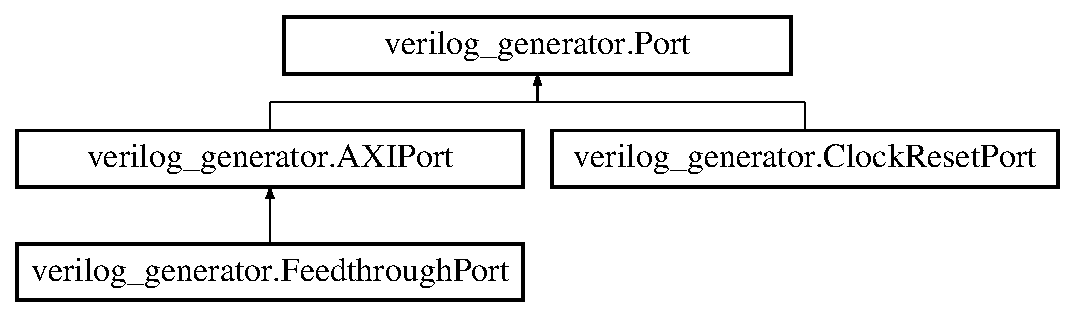
\includegraphics[height=3.000000cm]{classverilog__generator_1_1Port}
\end{center}
\end{figure}
\subsection*{Public Member Functions}
\begin{DoxyCompactItemize}
\item 
def \hyperlink{classverilog__generator_1_1Port_a7b2609c751eda67a2a7e35d8f57d75fd}{\-\_\-\-\_\-init\-\_\-\-\_\-}
\item 
def \hyperlink{classverilog__generator_1_1Port_ad3d21f70d7e366a31ad6fc97dbd2468e}{\-\_\-\-\_\-str\-\_\-\-\_\-}
\item 
def \hyperlink{classverilog__generator_1_1Port_a5987469ac2f49188cad0e77d288fdebe}{\-\_\-\-\_\-repr\-\_\-\-\_\-}
\item 
def \hyperlink{classverilog__generator_1_1Port_acedd4bff848ca18e07a04923fe9efba8}{\-\_\-\-\_\-invert\-\_\-\-\_\-}
\item 
def \hyperlink{classverilog__generator_1_1Port_a71569971a55c6a770c57f90a7a0a07b4}{flip\-\_\-direction}
\item 
def \hyperlink{classverilog__generator_1_1Port_a4c73cf8c4d9e342315e3e16d6903b492}{name}
\item 
def \hyperlink{classverilog__generator_1_1Port_a4c73cf8c4d9e342315e3e16d6903b492}{name}
\item 
def \hyperlink{classverilog__generator_1_1Port_a8b2b98d9a590fe243267303755fa6bd2}{port\-\_\-name}
\item 
def \hyperlink{classverilog__generator_1_1Port_ac99dae90da0d5a3d99e91955bad1cf86}{wire\-\_\-name}
\item 
def \hyperlink{classverilog__generator_1_1Port_a135b3a72ead7190ec7904431a0c493ec}{width\-\_\-str}
\item 
def \hyperlink{classverilog__generator_1_1Port_a543bcf22497b1223689dfa71ed628136}{array\-\_\-str}
\item 
def \hyperlink{classverilog__generator_1_1Port_aabb16d350aad41501088c31cdafb74cf}{display\-\_\-port}
\item 
def \hyperlink{classverilog__generator_1_1Port_a642131cb676f34f6001fae56e586d132}{display\-\_\-logic}
\item 
def \hyperlink{classverilog__generator_1_1Port_a178f35dae82ee7c28c186523a2686bd7}{set\-\_\-physical\-\_\-conn}
\end{DoxyCompactItemize}
\subsection*{Public Attributes}
\begin{DoxyCompactItemize}
\item 
\hyperlink{classverilog__generator_1_1Port_a7b2a8292d0545a4cf35ac056b2570d2e}{dir}
\item 
\hyperlink{classverilog__generator_1_1Port_aeae9d721aea818e4632e95841cfd3c9e}{dst}
\item 
\hyperlink{classverilog__generator_1_1Port_a628bc4ff9e6134c811e34bc9cd0b079c}{phy\-\_\-dst}
\item 
\hyperlink{classverilog__generator_1_1Port_a3f3622f36b1f3f9ee2318e94b79a55bb}{width}
\end{DoxyCompactItemize}
\subsection*{Static Public Attributes}
\begin{DoxyCompactItemize}
\item 
dictionary \hyperlink{classverilog__generator_1_1Port_a0ea87b8342a1ac4fe26ef336eab5c3cf}{dir2int} = \{\char`\"{}input\char`\"{}\-:0, \char`\"{}output\char`\"{}\-:1\}
\item 
dictionary \hyperlink{classverilog__generator_1_1Port_a32e2aa34b25401e3b4cdfe996d236d9b}{int2dir} = \{v\-:k for k, v in dir2int.\-items()\}
\item 
\hyperlink{classverilog__generator_1_1Port_a9f897dd8b1f10342ea181e7cf3d80af3}{self} = $\sim$self
\item 
string \hyperlink{classverilog__generator_1_1Port_aee949dd28d29fdbab884785abddc2e06}{end\-\_\-str} = \char`\"{}\char`\"{}
\item 
\hyperlink{classverilog__generator_1_1Port_aa1ecb52cdeafd852c6e6fb75c9c1b5b4}{x} = t3)
\end{DoxyCompactItemize}


\subsection{Constructor \& Destructor Documentation}
\hypertarget{classverilog__generator_1_1Port_a7b2609c751eda67a2a7e35d8f57d75fd}{\index{verilog\-\_\-generator\-::\-Port@{verilog\-\_\-generator\-::\-Port}!\-\_\-\-\_\-init\-\_\-\-\_\-@{\-\_\-\-\_\-init\-\_\-\-\_\-}}
\index{\-\_\-\-\_\-init\-\_\-\-\_\-@{\-\_\-\-\_\-init\-\_\-\-\_\-}!verilog_generator::Port@{verilog\-\_\-generator\-::\-Port}}
\subsubsection[{\-\_\-\-\_\-init\-\_\-\-\_\-}]{\setlength{\rightskip}{0pt plus 5cm}def verilog\-\_\-generator.\-Port.\-\_\-\-\_\-init\-\_\-\-\_\- (
\begin{DoxyParamCaption}
\item[{}]{self, }
\item[{}]{direction}
\end{DoxyParamCaption}
)}}\label{classverilog__generator_1_1Port_a7b2609c751eda67a2a7e35d8f57d75fd}


\subsection{Member Function Documentation}
\hypertarget{classverilog__generator_1_1Port_acedd4bff848ca18e07a04923fe9efba8}{\index{verilog\-\_\-generator\-::\-Port@{verilog\-\_\-generator\-::\-Port}!\-\_\-\-\_\-invert\-\_\-\-\_\-@{\-\_\-\-\_\-invert\-\_\-\-\_\-}}
\index{\-\_\-\-\_\-invert\-\_\-\-\_\-@{\-\_\-\-\_\-invert\-\_\-\-\_\-}!verilog_generator::Port@{verilog\-\_\-generator\-::\-Port}}
\subsubsection[{\-\_\-\-\_\-invert\-\_\-\-\_\-}]{\setlength{\rightskip}{0pt plus 5cm}def verilog\-\_\-generator.\-Port.\-\_\-\-\_\-invert\-\_\-\-\_\- (
\begin{DoxyParamCaption}
\item[{}]{self, }
\item[{}]{Port}
\end{DoxyParamCaption}
)}}\label{classverilog__generator_1_1Port_acedd4bff848ca18e07a04923fe9efba8}
\begin{DoxyVerb}negate a port changes the direction of the port
and also swap the src and destination
\end{DoxyVerb}
 \hypertarget{classverilog__generator_1_1Port_a5987469ac2f49188cad0e77d288fdebe}{\index{verilog\-\_\-generator\-::\-Port@{verilog\-\_\-generator\-::\-Port}!\-\_\-\-\_\-repr\-\_\-\-\_\-@{\-\_\-\-\_\-repr\-\_\-\-\_\-}}
\index{\-\_\-\-\_\-repr\-\_\-\-\_\-@{\-\_\-\-\_\-repr\-\_\-\-\_\-}!verilog_generator::Port@{verilog\-\_\-generator\-::\-Port}}
\subsubsection[{\-\_\-\-\_\-repr\-\_\-\-\_\-}]{\setlength{\rightskip}{0pt plus 5cm}def verilog\-\_\-generator.\-Port.\-\_\-\-\_\-repr\-\_\-\-\_\- (
\begin{DoxyParamCaption}
\item[{}]{self, }
\item[{}]{str}
\end{DoxyParamCaption}
)}}\label{classverilog__generator_1_1Port_a5987469ac2f49188cad0e77d288fdebe}
\hypertarget{classverilog__generator_1_1Port_ad3d21f70d7e366a31ad6fc97dbd2468e}{\index{verilog\-\_\-generator\-::\-Port@{verilog\-\_\-generator\-::\-Port}!\-\_\-\-\_\-str\-\_\-\-\_\-@{\-\_\-\-\_\-str\-\_\-\-\_\-}}
\index{\-\_\-\-\_\-str\-\_\-\-\_\-@{\-\_\-\-\_\-str\-\_\-\-\_\-}!verilog_generator::Port@{verilog\-\_\-generator\-::\-Port}}
\subsubsection[{\-\_\-\-\_\-str\-\_\-\-\_\-}]{\setlength{\rightskip}{0pt plus 5cm}def verilog\-\_\-generator.\-Port.\-\_\-\-\_\-str\-\_\-\-\_\- (
\begin{DoxyParamCaption}
\item[{}]{self, }
\item[{}]{str}
\end{DoxyParamCaption}
)}}\label{classverilog__generator_1_1Port_ad3d21f70d7e366a31ad6fc97dbd2468e}
\hypertarget{classverilog__generator_1_1Port_a543bcf22497b1223689dfa71ed628136}{\index{verilog\-\_\-generator\-::\-Port@{verilog\-\_\-generator\-::\-Port}!array\-\_\-str@{array\-\_\-str}}
\index{array\-\_\-str@{array\-\_\-str}!verilog_generator::Port@{verilog\-\_\-generator\-::\-Port}}
\subsubsection[{array\-\_\-str}]{\setlength{\rightskip}{0pt plus 5cm}def verilog\-\_\-generator.\-Port.\-array\-\_\-str (
\begin{DoxyParamCaption}
\item[{}]{self, }
\item[{}]{str}
\end{DoxyParamCaption}
)}}\label{classverilog__generator_1_1Port_a543bcf22497b1223689dfa71ed628136}
\begin{DoxyVerb}convert the array integer to a string that can be displayed in verilog port
declarations
\end{DoxyVerb}
 \hypertarget{classverilog__generator_1_1Port_a642131cb676f34f6001fae56e586d132}{\index{verilog\-\_\-generator\-::\-Port@{verilog\-\_\-generator\-::\-Port}!display\-\_\-logic@{display\-\_\-logic}}
\index{display\-\_\-logic@{display\-\_\-logic}!verilog_generator::Port@{verilog\-\_\-generator\-::\-Port}}
\subsubsection[{display\-\_\-logic}]{\setlength{\rightskip}{0pt plus 5cm}def verilog\-\_\-generator.\-Port.\-display\-\_\-logic (
\begin{DoxyParamCaption}
\item[{}]{self, }
\item[{}]{end}
\end{DoxyParamCaption}
)}}\label{classverilog__generator_1_1Port_a642131cb676f34f6001fae56e586d132}
\hypertarget{classverilog__generator_1_1Port_aabb16d350aad41501088c31cdafb74cf}{\index{verilog\-\_\-generator\-::\-Port@{verilog\-\_\-generator\-::\-Port}!display\-\_\-port@{display\-\_\-port}}
\index{display\-\_\-port@{display\-\_\-port}!verilog_generator::Port@{verilog\-\_\-generator\-::\-Port}}
\subsubsection[{display\-\_\-port}]{\setlength{\rightskip}{0pt plus 5cm}def verilog\-\_\-generator.\-Port.\-display\-\_\-port (
\begin{DoxyParamCaption}
\item[{}]{self, }
\item[{}]{end}
\end{DoxyParamCaption}
)}}\label{classverilog__generator_1_1Port_aabb16d350aad41501088c31cdafb74cf}
\hypertarget{classverilog__generator_1_1Port_a71569971a55c6a770c57f90a7a0a07b4}{\index{verilog\-\_\-generator\-::\-Port@{verilog\-\_\-generator\-::\-Port}!flip\-\_\-direction@{flip\-\_\-direction}}
\index{flip\-\_\-direction@{flip\-\_\-direction}!verilog_generator::Port@{verilog\-\_\-generator\-::\-Port}}
\subsubsection[{flip\-\_\-direction}]{\setlength{\rightskip}{0pt plus 5cm}def verilog\-\_\-generator.\-Port.\-flip\-\_\-direction (
\begin{DoxyParamCaption}
\item[{}]{self, }
\item[{}]{Port}
\end{DoxyParamCaption}
)}}\label{classverilog__generator_1_1Port_a71569971a55c6a770c57f90a7a0a07b4}
\hypertarget{classverilog__generator_1_1Port_a4c73cf8c4d9e342315e3e16d6903b492}{\index{verilog\-\_\-generator\-::\-Port@{verilog\-\_\-generator\-::\-Port}!name@{name}}
\index{name@{name}!verilog_generator::Port@{verilog\-\_\-generator\-::\-Port}}
\subsubsection[{name}]{\setlength{\rightskip}{0pt plus 5cm}def verilog\-\_\-generator.\-Port.\-name (
\begin{DoxyParamCaption}
\item[{}]{self, }
\item[{}]{str}
\end{DoxyParamCaption}
)}}\label{classverilog__generator_1_1Port_a4c73cf8c4d9e342315e3e16d6903b492}
\hypertarget{classverilog__generator_1_1Port_a4c73cf8c4d9e342315e3e16d6903b492}{\index{verilog\-\_\-generator\-::\-Port@{verilog\-\_\-generator\-::\-Port}!name@{name}}
\index{name@{name}!verilog_generator::Port@{verilog\-\_\-generator\-::\-Port}}
\subsubsection[{name}]{\setlength{\rightskip}{0pt plus 5cm}def verilog\-\_\-generator.\-Port.\-name (
\begin{DoxyParamCaption}
\item[{}]{self, }
\item[{}]{n, }
\item[{}]{None}
\end{DoxyParamCaption}
)}}\label{classverilog__generator_1_1Port_a4c73cf8c4d9e342315e3e16d6903b492}
\hypertarget{classverilog__generator_1_1Port_a8b2b98d9a590fe243267303755fa6bd2}{\index{verilog\-\_\-generator\-::\-Port@{verilog\-\_\-generator\-::\-Port}!port\-\_\-name@{port\-\_\-name}}
\index{port\-\_\-name@{port\-\_\-name}!verilog_generator::Port@{verilog\-\_\-generator\-::\-Port}}
\subsubsection[{port\-\_\-name}]{\setlength{\rightskip}{0pt plus 5cm}def verilog\-\_\-generator.\-Port.\-port\-\_\-name (
\begin{DoxyParamCaption}
\item[{}]{self, }
\item[{}]{str}
\end{DoxyParamCaption}
)}}\label{classverilog__generator_1_1Port_a8b2b98d9a590fe243267303755fa6bd2}
\hypertarget{classverilog__generator_1_1Port_a178f35dae82ee7c28c186523a2686bd7}{\index{verilog\-\_\-generator\-::\-Port@{verilog\-\_\-generator\-::\-Port}!set\-\_\-physical\-\_\-conn@{set\-\_\-physical\-\_\-conn}}
\index{set\-\_\-physical\-\_\-conn@{set\-\_\-physical\-\_\-conn}!verilog_generator::Port@{verilog\-\_\-generator\-::\-Port}}
\subsubsection[{set\-\_\-physical\-\_\-conn}]{\setlength{\rightskip}{0pt plus 5cm}def verilog\-\_\-generator.\-Port.\-set\-\_\-physical\-\_\-conn (
\begin{DoxyParamCaption}
\item[{}]{self, }
\item[{}]{module\-\_\-name, }
\item[{}]{modules, }
\item[{}]{None}
\end{DoxyParamCaption}
)}}\label{classverilog__generator_1_1Port_a178f35dae82ee7c28c186523a2686bd7}
\hypertarget{classverilog__generator_1_1Port_a135b3a72ead7190ec7904431a0c493ec}{\index{verilog\-\_\-generator\-::\-Port@{verilog\-\_\-generator\-::\-Port}!width\-\_\-str@{width\-\_\-str}}
\index{width\-\_\-str@{width\-\_\-str}!verilog_generator::Port@{verilog\-\_\-generator\-::\-Port}}
\subsubsection[{width\-\_\-str}]{\setlength{\rightskip}{0pt plus 5cm}def verilog\-\_\-generator.\-Port.\-width\-\_\-str (
\begin{DoxyParamCaption}
\item[{}]{self, }
\item[{}]{str}
\end{DoxyParamCaption}
)}}\label{classverilog__generator_1_1Port_a135b3a72ead7190ec7904431a0c493ec}
\begin{DoxyVerb}convert the width integer to a string that can be displayed in verilog port
declarations
\end{DoxyVerb}
 \hypertarget{classverilog__generator_1_1Port_ac99dae90da0d5a3d99e91955bad1cf86}{\index{verilog\-\_\-generator\-::\-Port@{verilog\-\_\-generator\-::\-Port}!wire\-\_\-name@{wire\-\_\-name}}
\index{wire\-\_\-name@{wire\-\_\-name}!verilog_generator::Port@{verilog\-\_\-generator\-::\-Port}}
\subsubsection[{wire\-\_\-name}]{\setlength{\rightskip}{0pt plus 5cm}def verilog\-\_\-generator.\-Port.\-wire\-\_\-name (
\begin{DoxyParamCaption}
\item[{}]{self, }
\item[{}]{str}
\end{DoxyParamCaption}
)}}\label{classverilog__generator_1_1Port_ac99dae90da0d5a3d99e91955bad1cf86}


\subsection{Member Data Documentation}
\hypertarget{classverilog__generator_1_1Port_a7b2a8292d0545a4cf35ac056b2570d2e}{\index{verilog\-\_\-generator\-::\-Port@{verilog\-\_\-generator\-::\-Port}!dir@{dir}}
\index{dir@{dir}!verilog_generator::Port@{verilog\-\_\-generator\-::\-Port}}
\subsubsection[{dir}]{\setlength{\rightskip}{0pt plus 5cm}verilog\-\_\-generator.\-Port.\-dir}}\label{classverilog__generator_1_1Port_a7b2a8292d0545a4cf35ac056b2570d2e}
\hypertarget{classverilog__generator_1_1Port_a0ea87b8342a1ac4fe26ef336eab5c3cf}{\index{verilog\-\_\-generator\-::\-Port@{verilog\-\_\-generator\-::\-Port}!dir2int@{dir2int}}
\index{dir2int@{dir2int}!verilog_generator::Port@{verilog\-\_\-generator\-::\-Port}}
\subsubsection[{dir2int}]{\setlength{\rightskip}{0pt plus 5cm}dictionary verilog\-\_\-generator.\-Port.\-dir2int = \{\char`\"{}input\char`\"{}\-:0, \char`\"{}output\char`\"{}\-:1\}\hspace{0.3cm}{\ttfamily [static]}}}\label{classverilog__generator_1_1Port_a0ea87b8342a1ac4fe26ef336eab5c3cf}
\hypertarget{classverilog__generator_1_1Port_aeae9d721aea818e4632e95841cfd3c9e}{\index{verilog\-\_\-generator\-::\-Port@{verilog\-\_\-generator\-::\-Port}!dst@{dst}}
\index{dst@{dst}!verilog_generator::Port@{verilog\-\_\-generator\-::\-Port}}
\subsubsection[{dst}]{\setlength{\rightskip}{0pt plus 5cm}verilog\-\_\-generator.\-Port.\-dst}}\label{classverilog__generator_1_1Port_aeae9d721aea818e4632e95841cfd3c9e}
\hypertarget{classverilog__generator_1_1Port_aee949dd28d29fdbab884785abddc2e06}{\index{verilog\-\_\-generator\-::\-Port@{verilog\-\_\-generator\-::\-Port}!end\-\_\-str@{end\-\_\-str}}
\index{end\-\_\-str@{end\-\_\-str}!verilog_generator::Port@{verilog\-\_\-generator\-::\-Port}}
\subsubsection[{end\-\_\-str}]{\setlength{\rightskip}{0pt plus 5cm}string verilog\-\_\-generator.\-Port.\-end\-\_\-str = \char`\"{}\char`\"{}\hspace{0.3cm}{\ttfamily [static]}}}\label{classverilog__generator_1_1Port_aee949dd28d29fdbab884785abddc2e06}
\hypertarget{classverilog__generator_1_1Port_a32e2aa34b25401e3b4cdfe996d236d9b}{\index{verilog\-\_\-generator\-::\-Port@{verilog\-\_\-generator\-::\-Port}!int2dir@{int2dir}}
\index{int2dir@{int2dir}!verilog_generator::Port@{verilog\-\_\-generator\-::\-Port}}
\subsubsection[{int2dir}]{\setlength{\rightskip}{0pt plus 5cm}dictionary verilog\-\_\-generator.\-Port.\-int2dir = \{v\-:k for k, v in dir2int.\-items()\}\hspace{0.3cm}{\ttfamily [static]}}}\label{classverilog__generator_1_1Port_a32e2aa34b25401e3b4cdfe996d236d9b}
\hypertarget{classverilog__generator_1_1Port_a628bc4ff9e6134c811e34bc9cd0b079c}{\index{verilog\-\_\-generator\-::\-Port@{verilog\-\_\-generator\-::\-Port}!phy\-\_\-dst@{phy\-\_\-dst}}
\index{phy\-\_\-dst@{phy\-\_\-dst}!verilog_generator::Port@{verilog\-\_\-generator\-::\-Port}}
\subsubsection[{phy\-\_\-dst}]{\setlength{\rightskip}{0pt plus 5cm}verilog\-\_\-generator.\-Port.\-phy\-\_\-dst}}\label{classverilog__generator_1_1Port_a628bc4ff9e6134c811e34bc9cd0b079c}
\hypertarget{classverilog__generator_1_1Port_a9f897dd8b1f10342ea181e7cf3d80af3}{\index{verilog\-\_\-generator\-::\-Port@{verilog\-\_\-generator\-::\-Port}!self@{self}}
\index{self@{self}!verilog_generator::Port@{verilog\-\_\-generator\-::\-Port}}
\subsubsection[{self}]{\setlength{\rightskip}{0pt plus 5cm}verilog\-\_\-generator.\-Port.\-self = $\sim$self\hspace{0.3cm}{\ttfamily [static]}}}\label{classverilog__generator_1_1Port_a9f897dd8b1f10342ea181e7cf3d80af3}
\hypertarget{classverilog__generator_1_1Port_a3f3622f36b1f3f9ee2318e94b79a55bb}{\index{verilog\-\_\-generator\-::\-Port@{verilog\-\_\-generator\-::\-Port}!width@{width}}
\index{width@{width}!verilog_generator::Port@{verilog\-\_\-generator\-::\-Port}}
\subsubsection[{width}]{\setlength{\rightskip}{0pt plus 5cm}verilog\-\_\-generator.\-Port.\-width}}\label{classverilog__generator_1_1Port_a3f3622f36b1f3f9ee2318e94b79a55bb}
\hypertarget{classverilog__generator_1_1Port_aa1ecb52cdeafd852c6e6fb75c9c1b5b4}{\index{verilog\-\_\-generator\-::\-Port@{verilog\-\_\-generator\-::\-Port}!x@{x}}
\index{x@{x}!verilog_generator::Port@{verilog\-\_\-generator\-::\-Port}}
\subsubsection[{x}]{\setlength{\rightskip}{0pt plus 5cm}verilog\-\_\-generator.\-Port.\-x = t3)\hspace{0.3cm}{\ttfamily [static]}}}\label{classverilog__generator_1_1Port_aa1ecb52cdeafd852c6e6fb75c9c1b5b4}


The documentation for this class was generated from the following file\-:\begin{DoxyCompactItemize}
\item 
\hyperlink{verilog__generator_8py}{verilog\-\_\-generator.\-py}\end{DoxyCompactItemize}

\hypertarget{classverilog__generator_1_1RegisterGenerationError}{\section{verilog\-\_\-generator.\-Register\-Generation\-Error Class Reference}
\label{classverilog__generator_1_1RegisterGenerationError}\index{verilog\-\_\-generator.\-Register\-Generation\-Error@{verilog\-\_\-generator.\-Register\-Generation\-Error}}
}
Inheritance diagram for verilog\-\_\-generator.\-Register\-Generation\-Error\-:\begin{figure}[H]
\begin{center}
\leavevmode
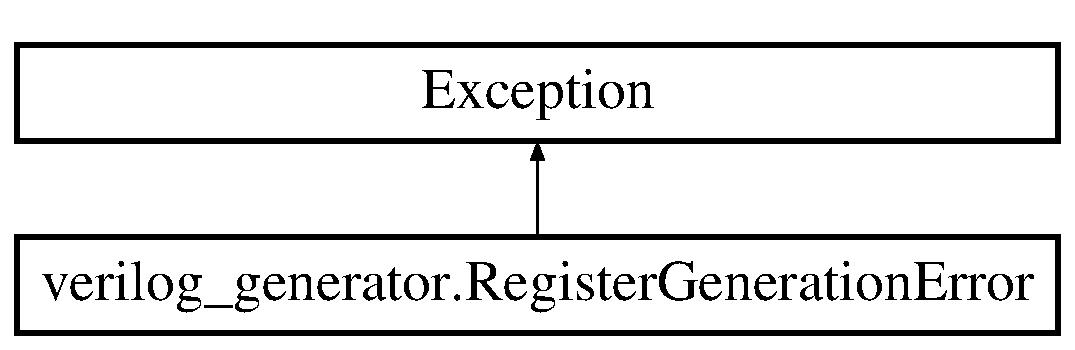
\includegraphics[height=2.000000cm]{classverilog__generator_1_1RegisterGenerationError}
\end{center}
\end{figure}


\subsection{Detailed Description}
\begin{DoxyVerb}Base class for other exceptions\end{DoxyVerb}
 

The documentation for this class was generated from the following file\-:\begin{DoxyCompactItemize}
\item 
\hyperlink{verilog__generator_8py}{verilog\-\_\-generator.\-py}\end{DoxyCompactItemize}

\hypertarget{classsrc_1_1spec__flow_1_1spec__flow}{\section{src.\-spec\-\_\-flow.\-spec\-\_\-flow Class Reference}
\label{classsrc_1_1spec__flow_1_1spec__flow}\index{src.\-spec\-\_\-flow.\-spec\-\_\-flow@{src.\-spec\-\_\-flow.\-spec\-\_\-flow}}
}


Spec flow to parse all the spec files and generate ports and params details.  


\subsection*{Public Member Functions}
\begin{DoxyCompactItemize}
\item 
def \hyperlink{classsrc_1_1spec__flow_1_1spec__flow_a6757af660d640f3b5d56d8e50fec66a6}{\-\_\-\-\_\-init\-\_\-\-\_\-}
\item 
def \hyperlink{classsrc_1_1spec__flow_1_1spec__flow_a756d1f4e2d357867a3080c7aa9c41af8}{dbg}
\begin{DoxyCompactList}\small\item\em Function to print a debug string in a debug dump file. \end{DoxyCompactList}\item 
def \hyperlink{classsrc_1_1spec__flow_1_1spec__flow_ab092eab2cfdda30353475676e0e22a4d}{find\-\_\-in\-\_\-files}
\begin{DoxyCompactList}\small\item\em Function to print a debug string in a debug dump file. \end{DoxyCompactList}\item 
def \hyperlink{classsrc_1_1spec__flow_1_1spec__flow_aca22fae70d0e3b3fa84853a03216bba8}{get\-\_\-module\-\_\-definition}
\begin{DoxyCompactList}\small\item\em Function to gather ports from spec flow. \end{DoxyCompactList}\end{DoxyCompactItemize}
\subsection*{Public Attributes}
\begin{DoxyCompactItemize}
\item 
\hyperlink{classsrc_1_1spec__flow_1_1spec__flow_ab03fdf31895e01ee5064a6e8c7770cf9}{interface\-\_\-spec\-\_\-files}
\item 
\hyperlink{classsrc_1_1spec__flow_1_1spec__flow_a6aa5ffd58e74b1bc405c03eb1f73685a}{interface\-\_\-def\-\_\-files}
\item 
\hyperlink{classsrc_1_1spec__flow_1_1spec__flow_ad353522556622de20c1ba3cab9437694}{module\-\_\-def\-\_\-files}
\item 
\hyperlink{classsrc_1_1spec__flow_1_1spec__flow_a20bffd81b17afc76d7147c31fb291c17}{module\-\_\-name}
\item 
\hyperlink{classsrc_1_1spec__flow_1_1spec__flow_a463c47bfa286d5b2b7335ac0055ffa21}{incl\-\_\-dirs}
\item 
\hyperlink{classsrc_1_1spec__flow_1_1spec__flow_a5c8040665b1b1bc870f26c389b9a0740}{files}
\item 
\hyperlink{classsrc_1_1spec__flow_1_1spec__flow_ae22e877e0abd24839a8a316275fd03c3}{debug}
\item 
\hyperlink{classsrc_1_1spec__flow_1_1spec__flow_ad84d4e7bcbad46bc04de94a068483821}{found\-\_\-error}
\item 
\hyperlink{classsrc_1_1spec__flow_1_1spec__flow_ae9d1bb1e24e85fc4396c5b58b1367163}{debug\-\_\-info}
\item 
\hyperlink{classsrc_1_1spec__flow_1_1spec__flow_ac0a0b21b31caeac8ad433e7b83a7a4b6}{module\-\_\-info}
\end{DoxyCompactItemize}


\subsection{Detailed Description}
Spec flow to parse all the spec files and generate ports and params details. 

\subsection{Constructor \& Destructor Documentation}
\hypertarget{classsrc_1_1spec__flow_1_1spec__flow_a6757af660d640f3b5d56d8e50fec66a6}{\index{src\-::spec\-\_\-flow\-::spec\-\_\-flow@{src\-::spec\-\_\-flow\-::spec\-\_\-flow}!\-\_\-\-\_\-init\-\_\-\-\_\-@{\-\_\-\-\_\-init\-\_\-\-\_\-}}
\index{\-\_\-\-\_\-init\-\_\-\-\_\-@{\-\_\-\-\_\-init\-\_\-\-\_\-}!src::spec_flow::spec_flow@{src\-::spec\-\_\-flow\-::spec\-\_\-flow}}
\subsubsection[{\-\_\-\-\_\-init\-\_\-\-\_\-}]{\setlength{\rightskip}{0pt plus 5cm}def src.\-spec\-\_\-flow.\-spec\-\_\-flow.\-\_\-\-\_\-init\-\_\-\-\_\- (
\begin{DoxyParamCaption}
\item[{}]{self, }
\item[{}]{if\-\_\-spec\-\_\-files, }
\item[{}]{if\-\_\-def\-\_\-files, }
\item[{}]{mod\-\_\-def\-\_\-files, }
\item[{}]{mod\-\_\-name, }
\item[{}]{incl\-\_\-dirs, }
\item[{}]{files, }
\item[{}]{debug\-\_\-en}
\end{DoxyParamCaption}
)}}\label{classsrc_1_1spec__flow_1_1spec__flow_a6757af660d640f3b5d56d8e50fec66a6}


\subsection{Member Function Documentation}
\hypertarget{classsrc_1_1spec__flow_1_1spec__flow_a756d1f4e2d357867a3080c7aa9c41af8}{\index{src\-::spec\-\_\-flow\-::spec\-\_\-flow@{src\-::spec\-\_\-flow\-::spec\-\_\-flow}!dbg@{dbg}}
\index{dbg@{dbg}!src::spec_flow::spec_flow@{src\-::spec\-\_\-flow\-::spec\-\_\-flow}}
\subsubsection[{dbg}]{\setlength{\rightskip}{0pt plus 5cm}def src.\-spec\-\_\-flow.\-spec\-\_\-flow.\-dbg (
\begin{DoxyParamCaption}
\item[{}]{self, }
\item[{}]{dbg\-\_\-info}
\end{DoxyParamCaption}
)}}\label{classsrc_1_1spec__flow_1_1spec__flow_a756d1f4e2d357867a3080c7aa9c41af8}


Function to print a debug string in a debug dump file. 

\hypertarget{classsrc_1_1spec__flow_1_1spec__flow_ab092eab2cfdda30353475676e0e22a4d}{\index{src\-::spec\-\_\-flow\-::spec\-\_\-flow@{src\-::spec\-\_\-flow\-::spec\-\_\-flow}!find\-\_\-in\-\_\-files@{find\-\_\-in\-\_\-files}}
\index{find\-\_\-in\-\_\-files@{find\-\_\-in\-\_\-files}!src::spec_flow::spec_flow@{src\-::spec\-\_\-flow\-::spec\-\_\-flow}}
\subsubsection[{find\-\_\-in\-\_\-files}]{\setlength{\rightskip}{0pt plus 5cm}def src.\-spec\-\_\-flow.\-spec\-\_\-flow.\-find\-\_\-in\-\_\-files (
\begin{DoxyParamCaption}
\item[{}]{self, }
\item[{}]{filename}
\end{DoxyParamCaption}
)}}\label{classsrc_1_1spec__flow_1_1spec__flow_ab092eab2cfdda30353475676e0e22a4d}


Function to print a debug string in a debug dump file. 

\hypertarget{classsrc_1_1spec__flow_1_1spec__flow_aca22fae70d0e3b3fa84853a03216bba8}{\index{src\-::spec\-\_\-flow\-::spec\-\_\-flow@{src\-::spec\-\_\-flow\-::spec\-\_\-flow}!get\-\_\-module\-\_\-definition@{get\-\_\-module\-\_\-definition}}
\index{get\-\_\-module\-\_\-definition@{get\-\_\-module\-\_\-definition}!src::spec_flow::spec_flow@{src\-::spec\-\_\-flow\-::spec\-\_\-flow}}
\subsubsection[{get\-\_\-module\-\_\-definition}]{\setlength{\rightskip}{0pt plus 5cm}def src.\-spec\-\_\-flow.\-spec\-\_\-flow.\-get\-\_\-module\-\_\-definition (
\begin{DoxyParamCaption}
\item[{}]{self}
\end{DoxyParamCaption}
)}}\label{classsrc_1_1spec__flow_1_1spec__flow_aca22fae70d0e3b3fa84853a03216bba8}


Function to gather ports from spec flow. 



\subsection{Member Data Documentation}
\hypertarget{classsrc_1_1spec__flow_1_1spec__flow_ae22e877e0abd24839a8a316275fd03c3}{\index{src\-::spec\-\_\-flow\-::spec\-\_\-flow@{src\-::spec\-\_\-flow\-::spec\-\_\-flow}!debug@{debug}}
\index{debug@{debug}!src::spec_flow::spec_flow@{src\-::spec\-\_\-flow\-::spec\-\_\-flow}}
\subsubsection[{debug}]{\setlength{\rightskip}{0pt plus 5cm}src.\-spec\-\_\-flow.\-spec\-\_\-flow.\-debug}}\label{classsrc_1_1spec__flow_1_1spec__flow_ae22e877e0abd24839a8a316275fd03c3}
\hypertarget{classsrc_1_1spec__flow_1_1spec__flow_ae9d1bb1e24e85fc4396c5b58b1367163}{\index{src\-::spec\-\_\-flow\-::spec\-\_\-flow@{src\-::spec\-\_\-flow\-::spec\-\_\-flow}!debug\-\_\-info@{debug\-\_\-info}}
\index{debug\-\_\-info@{debug\-\_\-info}!src::spec_flow::spec_flow@{src\-::spec\-\_\-flow\-::spec\-\_\-flow}}
\subsubsection[{debug\-\_\-info}]{\setlength{\rightskip}{0pt plus 5cm}src.\-spec\-\_\-flow.\-spec\-\_\-flow.\-debug\-\_\-info}}\label{classsrc_1_1spec__flow_1_1spec__flow_ae9d1bb1e24e85fc4396c5b58b1367163}
\hypertarget{classsrc_1_1spec__flow_1_1spec__flow_a5c8040665b1b1bc870f26c389b9a0740}{\index{src\-::spec\-\_\-flow\-::spec\-\_\-flow@{src\-::spec\-\_\-flow\-::spec\-\_\-flow}!files@{files}}
\index{files@{files}!src::spec_flow::spec_flow@{src\-::spec\-\_\-flow\-::spec\-\_\-flow}}
\subsubsection[{files}]{\setlength{\rightskip}{0pt plus 5cm}src.\-spec\-\_\-flow.\-spec\-\_\-flow.\-files}}\label{classsrc_1_1spec__flow_1_1spec__flow_a5c8040665b1b1bc870f26c389b9a0740}
\hypertarget{classsrc_1_1spec__flow_1_1spec__flow_ad84d4e7bcbad46bc04de94a068483821}{\index{src\-::spec\-\_\-flow\-::spec\-\_\-flow@{src\-::spec\-\_\-flow\-::spec\-\_\-flow}!found\-\_\-error@{found\-\_\-error}}
\index{found\-\_\-error@{found\-\_\-error}!src::spec_flow::spec_flow@{src\-::spec\-\_\-flow\-::spec\-\_\-flow}}
\subsubsection[{found\-\_\-error}]{\setlength{\rightskip}{0pt plus 5cm}src.\-spec\-\_\-flow.\-spec\-\_\-flow.\-found\-\_\-error}}\label{classsrc_1_1spec__flow_1_1spec__flow_ad84d4e7bcbad46bc04de94a068483821}
\hypertarget{classsrc_1_1spec__flow_1_1spec__flow_a463c47bfa286d5b2b7335ac0055ffa21}{\index{src\-::spec\-\_\-flow\-::spec\-\_\-flow@{src\-::spec\-\_\-flow\-::spec\-\_\-flow}!incl\-\_\-dirs@{incl\-\_\-dirs}}
\index{incl\-\_\-dirs@{incl\-\_\-dirs}!src::spec_flow::spec_flow@{src\-::spec\-\_\-flow\-::spec\-\_\-flow}}
\subsubsection[{incl\-\_\-dirs}]{\setlength{\rightskip}{0pt plus 5cm}src.\-spec\-\_\-flow.\-spec\-\_\-flow.\-incl\-\_\-dirs}}\label{classsrc_1_1spec__flow_1_1spec__flow_a463c47bfa286d5b2b7335ac0055ffa21}
\hypertarget{classsrc_1_1spec__flow_1_1spec__flow_a6aa5ffd58e74b1bc405c03eb1f73685a}{\index{src\-::spec\-\_\-flow\-::spec\-\_\-flow@{src\-::spec\-\_\-flow\-::spec\-\_\-flow}!interface\-\_\-def\-\_\-files@{interface\-\_\-def\-\_\-files}}
\index{interface\-\_\-def\-\_\-files@{interface\-\_\-def\-\_\-files}!src::spec_flow::spec_flow@{src\-::spec\-\_\-flow\-::spec\-\_\-flow}}
\subsubsection[{interface\-\_\-def\-\_\-files}]{\setlength{\rightskip}{0pt plus 5cm}src.\-spec\-\_\-flow.\-spec\-\_\-flow.\-interface\-\_\-def\-\_\-files}}\label{classsrc_1_1spec__flow_1_1spec__flow_a6aa5ffd58e74b1bc405c03eb1f73685a}
\hypertarget{classsrc_1_1spec__flow_1_1spec__flow_ab03fdf31895e01ee5064a6e8c7770cf9}{\index{src\-::spec\-\_\-flow\-::spec\-\_\-flow@{src\-::spec\-\_\-flow\-::spec\-\_\-flow}!interface\-\_\-spec\-\_\-files@{interface\-\_\-spec\-\_\-files}}
\index{interface\-\_\-spec\-\_\-files@{interface\-\_\-spec\-\_\-files}!src::spec_flow::spec_flow@{src\-::spec\-\_\-flow\-::spec\-\_\-flow}}
\subsubsection[{interface\-\_\-spec\-\_\-files}]{\setlength{\rightskip}{0pt plus 5cm}src.\-spec\-\_\-flow.\-spec\-\_\-flow.\-interface\-\_\-spec\-\_\-files}}\label{classsrc_1_1spec__flow_1_1spec__flow_ab03fdf31895e01ee5064a6e8c7770cf9}
\hypertarget{classsrc_1_1spec__flow_1_1spec__flow_ad353522556622de20c1ba3cab9437694}{\index{src\-::spec\-\_\-flow\-::spec\-\_\-flow@{src\-::spec\-\_\-flow\-::spec\-\_\-flow}!module\-\_\-def\-\_\-files@{module\-\_\-def\-\_\-files}}
\index{module\-\_\-def\-\_\-files@{module\-\_\-def\-\_\-files}!src::spec_flow::spec_flow@{src\-::spec\-\_\-flow\-::spec\-\_\-flow}}
\subsubsection[{module\-\_\-def\-\_\-files}]{\setlength{\rightskip}{0pt plus 5cm}src.\-spec\-\_\-flow.\-spec\-\_\-flow.\-module\-\_\-def\-\_\-files}}\label{classsrc_1_1spec__flow_1_1spec__flow_ad353522556622de20c1ba3cab9437694}
\hypertarget{classsrc_1_1spec__flow_1_1spec__flow_ac0a0b21b31caeac8ad433e7b83a7a4b6}{\index{src\-::spec\-\_\-flow\-::spec\-\_\-flow@{src\-::spec\-\_\-flow\-::spec\-\_\-flow}!module\-\_\-info@{module\-\_\-info}}
\index{module\-\_\-info@{module\-\_\-info}!src::spec_flow::spec_flow@{src\-::spec\-\_\-flow\-::spec\-\_\-flow}}
\subsubsection[{module\-\_\-info}]{\setlength{\rightskip}{0pt plus 5cm}src.\-spec\-\_\-flow.\-spec\-\_\-flow.\-module\-\_\-info}}\label{classsrc_1_1spec__flow_1_1spec__flow_ac0a0b21b31caeac8ad433e7b83a7a4b6}
\hypertarget{classsrc_1_1spec__flow_1_1spec__flow_a20bffd81b17afc76d7147c31fb291c17}{\index{src\-::spec\-\_\-flow\-::spec\-\_\-flow@{src\-::spec\-\_\-flow\-::spec\-\_\-flow}!module\-\_\-name@{module\-\_\-name}}
\index{module\-\_\-name@{module\-\_\-name}!src::spec_flow::spec_flow@{src\-::spec\-\_\-flow\-::spec\-\_\-flow}}
\subsubsection[{module\-\_\-name}]{\setlength{\rightskip}{0pt plus 5cm}src.\-spec\-\_\-flow.\-spec\-\_\-flow.\-module\-\_\-name}}\label{classsrc_1_1spec__flow_1_1spec__flow_a20bffd81b17afc76d7147c31fb291c17}


The documentation for this class was generated from the following file\-:\begin{DoxyCompactItemize}
\item 
src/\hyperlink{spec__flow_8py}{spec\-\_\-flow.\-py}\end{DoxyCompactItemize}

\hypertarget{classsrc_1_1verilog__parser_1_1verilog__parser}{\section{src.\-verilog\-\_\-parser.\-verilog\-\_\-parser Class Reference}
\label{classsrc_1_1verilog__parser_1_1verilog__parser}\index{src.\-verilog\-\_\-parser.\-verilog\-\_\-parser@{src.\-verilog\-\_\-parser.\-verilog\-\_\-parser}}
}
\subsection*{Public Member Functions}
\begin{DoxyCompactItemize}
\item 
def \hyperlink{classsrc_1_1verilog__parser_1_1verilog__parser_a5841508e2d8cfccaebfe162fe72e4d03}{\-\_\-\-\_\-init\-\_\-\-\_\-}
\item 
def \hyperlink{classsrc_1_1verilog__parser_1_1verilog__parser_acb8bc8dd21dc57dd3562f02efc76b7be}{dbg\-\_\-store}
\begin{DoxyCompactList}\small\item\em Loading S\-V packages. \end{DoxyCompactList}\item 
def \hyperlink{classsrc_1_1verilog__parser_1_1verilog__parser_a9458eb4df7beb0eda268a69b82f6e379}{dbg}
\item 
def \hyperlink{classsrc_1_1verilog__parser_1_1verilog__parser_a27b563239157cc0e3e8b41ae3b141280}{get\-\_\-ports}
\item 
def \hyperlink{classsrc_1_1verilog__parser_1_1verilog__parser_a6a35e0559edeb8429687caa189b15fe5}{clog2}
\item 
def \hyperlink{classsrc_1_1verilog__parser_1_1verilog__parser_ae00350e04e9bc19aa31e843c571361d2}{find\-\_\-manual\-\_\-submod}
\item 
def \hyperlink{classsrc_1_1verilog__parser_1_1verilog__parser_a2266112da05de7273c1f91d5a3148d51}{check\-\_\-for\-\_\-bracket}
\item 
def \hyperlink{classsrc_1_1verilog__parser_1_1verilog__parser_ae54a1ce303f44299d7ba906d1354e7d1}{binding\-\_\-typedef}
\item 
def \hyperlink{classsrc_1_1verilog__parser_1_1verilog__parser_a922d64b3c8d19d0833a91fe5dfaedc23}{check\-\_\-if\-\_\-parsing\-\_\-needed}
\item 
def \hyperlink{classsrc_1_1verilog__parser_1_1verilog__parser_a7837590371670e9004e352a113fe1f6c}{parse\-\_\-assignments}
\item 
def \hyperlink{classsrc_1_1verilog__parser_1_1verilog__parser_ab19b03c5107d2fd791943e2be1406f7c}{parse\-\_\-case\-\_\-expression}
\item 
def \hyperlink{classsrc_1_1verilog__parser_1_1verilog__parser_a8f7f47527e55b31f7ab1df9ec367a4b2}{parse\-\_\-conditions}
\item 
def \hyperlink{classsrc_1_1verilog__parser_1_1verilog__parser_a72fe0b75d740cfef1a00add06ab7e0f3}{update\-\_\-typedef\-\_\-regs}
\item 
def \hyperlink{classsrc_1_1verilog__parser_1_1verilog__parser_a7e91de6d83fd6e012fef8cf42b886a34}{parse\-\_\-signal}
\item 
def \hyperlink{classsrc_1_1verilog__parser_1_1verilog__parser_a6c20c3d036a8846c2d2b398857809799}{update\-\_\-wire\-\_\-reg\-\_\-signal\-\_\-lists}
\item 
def \hyperlink{classsrc_1_1verilog__parser_1_1verilog__parser_aa66877c2836dbc313769721d74b86d78}{update\-\_\-bitdef}
\item 
def \hyperlink{classsrc_1_1verilog__parser_1_1verilog__parser_a4c232a34556813fb83cf4e14170e243e}{remove\-\_\-outside\-\_\-sqbrackets}
\item 
def \hyperlink{classsrc_1_1verilog__parser_1_1verilog__parser_a5061b79dd42f4941f315596484034eb6}{parse\-\_\-reg\-\_\-wire\-\_\-logic}
\item 
def \hyperlink{classsrc_1_1verilog__parser_1_1verilog__parser_afc2edb01505646fb4767d3d3beef78b7}{parse\-\_\-ios}
\item 
def \hyperlink{classsrc_1_1verilog__parser_1_1verilog__parser_a74ba467aaa37c811d43ec9a3d91d6fdf}{load\-\_\-import\-\_\-or\-\_\-include\-\_\-file}
\item 
def \hyperlink{classsrc_1_1verilog__parser_1_1verilog__parser_a1d1e764b68f2b25dcbcb8e8f80c5d297}{parse\-\_\-struct\-\_\-union}
\item 
def \hyperlink{classsrc_1_1verilog__parser_1_1verilog__parser_aedc7d876db9e8de117176e47d47242e4}{param\-\_\-proc}
\item 
def \hyperlink{classsrc_1_1verilog__parser_1_1verilog__parser_a1df1568e05ae1717e28010a4a7019be2}{enums\-\_\-proc}
\item 
def \hyperlink{classsrc_1_1verilog__parser_1_1verilog__parser_a04495de1d32401dd5b7d8b112f171411}{tick\-\_\-ifdef\-\_\-proc}
\item 
def \hyperlink{classsrc_1_1verilog__parser_1_1verilog__parser_a2ac6051f26cee8fc4890f94fa32fa287}{sub\-\_\-tick\-\_\-ifdef\-\_\-proc}
\item 
def \hyperlink{classsrc_1_1verilog__parser_1_1verilog__parser_adbfb593949354e4adfba57e620f37e48}{tick\-\_\-def\-\_\-proc}
\item 
def \hyperlink{classsrc_1_1verilog__parser_1_1verilog__parser_aae3b515116fb91e32af6fc95c796cc2c}{get\-\_\-tick\-\_\-defval}
\item 
def \hyperlink{classsrc_1_1verilog__parser_1_1verilog__parser_ac38cf01d9a31f8d653941b74dbe7cfa2}{get\-\_\-param}
\item 
def \hyperlink{classsrc_1_1verilog__parser_1_1verilog__parser_a21984185944e7ca6cab073280d7ee249}{replace\-\_\-clog2}
\item 
def \hyperlink{classsrc_1_1verilog__parser_1_1verilog__parser_a188246bedacf825272b491e14d8c2ba3}{get\-\_\-dollar\-\_\-bits\-\_\-val}
\item 
def \hyperlink{classsrc_1_1verilog__parser_1_1verilog__parser_a335ab7ed6e9f856a7df251dd34725762}{tickdef\-\_\-param\-\_\-getval}
\item 
def \hyperlink{classsrc_1_1verilog__parser_1_1verilog__parser_a2cce56162afd3054e1a50c226c90e9ee}{split\-\_\-on\-\_\-word\-\_\-boundary}
\item 
def \hyperlink{classsrc_1_1verilog__parser_1_1verilog__parser_a7fed4bff4433384050175e0753d61a00}{find\-\_\-in\-\_\-files}
\item 
def \hyperlink{classsrc_1_1verilog__parser_1_1verilog__parser_a2ed049ecaa016db28e68c585938be4a9}{parse\-\_\-verilog}
\end{DoxyCompactItemize}
\subsection*{Public Attributes}
\begin{DoxyCompactItemize}
\item 
\hyperlink{classsrc_1_1verilog__parser_1_1verilog__parser_a517fc26126209e45aa5eefee4e937fd5}{module\-\_\-name}
\begin{DoxyCompactList}\small\item\em Parameter parsing. \end{DoxyCompactList}\item 
\hyperlink{classsrc_1_1verilog__parser_1_1verilog__parser_ae7207d3f921f1717d4c75b105beb3bd9}{parse\-\_\-lines}
\item 
\hyperlink{classsrc_1_1verilog__parser_1_1verilog__parser_a0fac67c4c5969d90e8b49edd665d9677}{incl\-\_\-dirs}
\item 
\hyperlink{classsrc_1_1verilog__parser_1_1verilog__parser_a7f17d4fbfa695ef7dd9a846135434690}{files}
\item 
\hyperlink{classsrc_1_1verilog__parser_1_1verilog__parser_a32cec6a447990615389a8cf249caa57c}{package\-\_\-files}
\item 
\hyperlink{classsrc_1_1verilog__parser_1_1verilog__parser_add046555471f9fe5a92518cf17462e38}{hash\-\_\-defines}
\item 
\hyperlink{classsrc_1_1verilog__parser_1_1verilog__parser_a1f81b9bfb1e1f5bf5819d26689b5a177}{parsing\-\_\-format}
\begin{DoxyCompactList}\small\item\em Manual declarations. \end{DoxyCompactList}\item 
\hyperlink{classsrc_1_1verilog__parser_1_1verilog__parser_a08e67f9ef0de0181a10caacaec6116d5}{debug}
\item 
\hyperlink{classsrc_1_1verilog__parser_1_1verilog__parser_ac8668d7328c5a15f7d67ede379b30ea3}{debug\-\_\-file}
\item 
\hyperlink{classsrc_1_1verilog__parser_1_1verilog__parser_afdfce44cfa00c4603ac52ef06cfbaeed}{verilog\-\_\-define\-\_\-files}
\item 
\hyperlink{classsrc_1_1verilog__parser_1_1verilog__parser_abdf606fe7e29eadd46bbefe59cc4ae2a}{parser\-\_\-on}
\item 
\hyperlink{classsrc_1_1verilog__parser_1_1verilog__parser_a2f62555a692365df5e08fda3b4869c82}{debug\-\_\-print}
\item 
\hyperlink{classsrc_1_1verilog__parser_1_1verilog__parser_aef575793938cd682ab9b35ef0f954d2c}{generate\-\_\-stub}
\item 
\hyperlink{classsrc_1_1verilog__parser_1_1verilog__parser_a54f0c4a4380a1b9bbdccd108cba9d08f}{parse\-\_\-generate}
\item 
\hyperlink{classsrc_1_1verilog__parser_1_1verilog__parser_a9ca2637cb2fee2c2cc14bef5cefbc55c}{gen\-\_\-dependencies}
\item 
\hyperlink{classsrc_1_1verilog__parser_1_1verilog__parser_a155e7b6f4cfd1a3f02dd900e642cac73}{interface\-\_\-spec\-\_\-files}
\item 
\hyperlink{classsrc_1_1verilog__parser_1_1verilog__parser_aa65e2df4339514dfd088c76ab9306c97}{interface\-\_\-def\-\_\-files}
\item 
\hyperlink{classsrc_1_1verilog__parser_1_1verilog__parser_a3db0cd72db1ddba2c6048d6fece48a34}{module\-\_\-def\-\_\-files}
\item 
\hyperlink{classsrc_1_1verilog__parser_1_1verilog__parser_a78034c322e8a3f31bdac403da9977fcb}{auto\-\_\-package\-\_\-load}
\item 
\hyperlink{classsrc_1_1verilog__parser_1_1verilog__parser_ab6f63afce27653ad48fc243e234c0c29}{clock}
\item 
\hyperlink{classsrc_1_1verilog__parser_1_1verilog__parser_a425456e33f633ca2cbfb13bd2fd05c4f}{async\-\_\-reset}
\item 
\hyperlink{classsrc_1_1verilog__parser_1_1verilog__parser_ae7f406445a30521eda2e92708fa64bae}{sync\-\_\-reset}
\item 
\hyperlink{classsrc_1_1verilog__parser_1_1verilog__parser_a9a7aaf735718fa08e9e442ded25bd33c}{reset\-\_\-type}
\item 
\hyperlink{classsrc_1_1verilog__parser_1_1verilog__parser_aad5fd2ecca89fc5793a69c2d97fdeb8e}{tick\-\_\-defines}
\item 
\hyperlink{classsrc_1_1verilog__parser_1_1verilog__parser_ad6e63fac0c5ab3d3c9ff0ffd7e966fe3}{tick\-\_\-ifdef\-\_\-dis}
\item 
\hyperlink{classsrc_1_1verilog__parser_1_1verilog__parser_a7693c6d544636962a754d3781b3246f9}{tick\-\_\-ifdef\-\_\-en}
\begin{DoxyCompactList}\small\item\em \&Parser\-Off and \&Skip\-End for parsing skip \end{DoxyCompactList}\item 
\hyperlink{classsrc_1_1verilog__parser_1_1verilog__parser_a18f0a3d7b00dc045a831a4c852cb81a9}{tick\-\_\-decisions}
\item 
\hyperlink{classsrc_1_1verilog__parser_1_1verilog__parser_a2f7dedc04e4a32968765ac354243f907}{tick\-\_\-types}
\item 
\hyperlink{classsrc_1_1verilog__parser_1_1verilog__parser_a648196e70fb7e82ac29ab300a162d055}{tick\-\_\-served}
\item 
\hyperlink{classsrc_1_1verilog__parser_1_1verilog__parser_a0c1a032cbfb2282c87c68f1670399c0d}{tick\-\_\-curr\-\_\-decision}
\item 
\hyperlink{classsrc_1_1verilog__parser_1_1verilog__parser_a09e28ad43e48089e1f58d1b858aa5fa2}{tick\-\_\-curr\-\_\-type}
\item 
\hyperlink{classsrc_1_1verilog__parser_1_1verilog__parser_a4a833b74a2be85c3719261328722e371}{tick\-\_\-curr\-\_\-served}
\item 
\hyperlink{classsrc_1_1verilog__parser_1_1verilog__parser_a942af18cb73658579b4a9c277086f3cd}{last\-\_\-tick\-\_\-loc}
\item 
\hyperlink{classsrc_1_1verilog__parser_1_1verilog__parser_a12004b8cf62949956ae314ef476dab87}{packages}
\item 
\hyperlink{classsrc_1_1verilog__parser_1_1verilog__parser_a47eeccd54b5c7c35a8836faaf6a9bde7}{classes}
\item 
\hyperlink{classsrc_1_1verilog__parser_1_1verilog__parser_a7c108505c58a79df46601966e54a23db}{params}
\item 
\hyperlink{classsrc_1_1verilog__parser_1_1verilog__parser_a1c9d4e2a68d2cfefb74f0d4a4ff9d3e7}{typedef\-\_\-enums}
\item 
\hyperlink{classsrc_1_1verilog__parser_1_1verilog__parser_a523203cbac7ad76b0c193c4ab57c1ff8}{typedef\-\_\-logics}
\item 
\hyperlink{classsrc_1_1verilog__parser_1_1verilog__parser_a2f3d97d651c6748ef49e137c39a88613}{typedef\-\_\-structs}
\item 
\hyperlink{classsrc_1_1verilog__parser_1_1verilog__parser_a72b450cd8097ca7d0b7f63acb4d4c281}{typedef\-\_\-unions}
\item 
\hyperlink{classsrc_1_1verilog__parser_1_1verilog__parser_ac58bfda0c6c3b46dddf4965f0fbf818f}{typedef\-\_\-bindings}
\item 
\hyperlink{classsrc_1_1verilog__parser_1_1verilog__parser_a3a27f85383ea07970dbccc29bc68ea06}{manual\-\_\-ports}
\item 
\hyperlink{classsrc_1_1verilog__parser_1_1verilog__parser_a259774d2a3cc74fd78518fcaabf3867e}{found\-\_\-error}
\begin{DoxyCompactList}\small\item\em `ifdef/ifndef/elif/else/endif processing \end{DoxyCompactList}\item 
\hyperlink{classsrc_1_1verilog__parser_1_1verilog__parser_ad751d762895cd27ae3de7b4adb34ee29}{auto\-\_\-reset\-\_\-val}
\item 
\hyperlink{classsrc_1_1verilog__parser_1_1verilog__parser_ac977e4adc51ad4604b1cb0c4f722d7ba}{sub\-\_\-last\-\_\-tick\-\_\-loc}
\item 
\hyperlink{classsrc_1_1verilog__parser_1_1verilog__parser_a3ab09c605608b1763a9d38d858598d1e}{sub\-\_\-tick\-\_\-curr\-\_\-served}
\item 
\hyperlink{classsrc_1_1verilog__parser_1_1verilog__parser_a31e7135de174cf37f497d1197f82b783}{sub\-\_\-tick\-\_\-curr\-\_\-decision}
\item 
\hyperlink{classsrc_1_1verilog__parser_1_1verilog__parser_abfb69b08a6d614d5c0da76f670f9047b}{sub\-\_\-tick\-\_\-curr\-\_\-type}
\item 
\hyperlink{classsrc_1_1verilog__parser_1_1verilog__parser_af8c49dd8d8b401c3a2eee7489ffa04e9}{line}
\item 
\hyperlink{classsrc_1_1verilog__parser_1_1verilog__parser_a33892150ed346c986314e42e8000c838}{line\-\_\-no}
\item 
\hyperlink{classsrc_1_1verilog__parser_1_1verilog__parser_a5233a3fc04bd927335ca10b2ff05e5f2}{original\-\_\-line}
\item 
\hyperlink{classsrc_1_1verilog__parser_1_1verilog__parser_a22d4873848308efa676a094cf71164fa}{pkg2assign\-\_\-index}
\begin{DoxyCompactList}\small\item\em Assertions Skip. \end{DoxyCompactList}\item 
\hyperlink{classsrc_1_1verilog__parser_1_1verilog__parser_a1182cf00e893bc40e432fefe69df4b7b}{assign2pkg\-\_\-index}
\item 
\hyperlink{classsrc_1_1verilog__parser_1_1verilog__parser_ab5ccb54f6c07eed5f249a6f7d736121c}{always\-\_\-constructs}
\begin{DoxyCompactList}\small\item\em Generate Skip \& Parsing. \end{DoxyCompactList}\item 
\hyperlink{classsrc_1_1verilog__parser_1_1verilog__parser_ae62ba26ec0f8a70e7feacd7546bac025}{generate\-\_\-for\-\_\-loops}
\item 
\hyperlink{classsrc_1_1verilog__parser_1_1verilog__parser_af691444ec4ff5f2e93254ed9b5dffdf3}{generate\-\_\-for\-\_\-loop\-\_\-count}
\begin{DoxyCompactList}\small\item\em for loop processing \end{DoxyCompactList}\item 
\hyperlink{classsrc_1_1verilog__parser_1_1verilog__parser_ab2bdbf68ed106816c50e5845c26bbe67}{package\-\_\-name}
\begin{DoxyCompactList}\small\item\em typedef logic extraction \end{DoxyCompactList}\item 
\hyperlink{classsrc_1_1verilog__parser_1_1verilog__parser_a54670377536cff31d6b6638278eeb5d5}{class\-\_\-name}
\begin{DoxyCompactList}\small\item\em class and endclass \end{DoxyCompactList}\item 
\hyperlink{classsrc_1_1verilog__parser_1_1verilog__parser_a833a3acd432dbf02d6c9f4333bcafba2}{module\-\_\-param\-\_\-line}
\begin{DoxyCompactList}\small\item\em Detect typedef usages. \end{DoxyCompactList}\item 
\hyperlink{classsrc_1_1verilog__parser_1_1verilog__parser_a9e6de26b5fd6ad1ab65b4ed97cd6c078}{module\-\_\-info}
\begin{DoxyCompactList}\small\item\em Load parameters and I\-Os from module spec. \end{DoxyCompactList}\item 
\hyperlink{classsrc_1_1verilog__parser_1_1verilog__parser_afbe4a23f0db34f027628a4f5a9b5f7d2}{module\-\_\-found}
\begin{DoxyCompactList}\small\item\em Loading the module dependencies with spec files list. \end{DoxyCompactList}\item 
\hyperlink{classsrc_1_1verilog__parser_1_1verilog__parser_ac292954891b0eda38bc1272e74b71bf5}{auto\-\_\-reset\-\_\-en}
\begin{DoxyCompactList}\small\item\em \&Posedge, \&Negedge, \&Clock, \&Sync\-Reset and \&Asyncreset \end{DoxyCompactList}\item 
\hyperlink{classsrc_1_1verilog__parser_1_1verilog__parser_af94b1eb70c83858b118ac5f6fd150abb}{auto\-\_\-reset\-\_\-index}
\item 
\hyperlink{classsrc_1_1verilog__parser_1_1verilog__parser_a7d3f4749a1f69f8a1cf2c00b4d96f82e}{always\-\_\-for\-\_\-loop\-\_\-count}
\begin{DoxyCompactList}\small\item\em Error out if R\-T\-L uses casex that is not allowed. \end{DoxyCompactList}\item 
\hyperlink{classsrc_1_1verilog__parser_1_1verilog__parser_a0fe75e02462dff88651e209020bd8c08}{sub\-\_\-tick\-\_\-defines}
\begin{DoxyCompactList}\small\item\em Auto Instantiation. \end{DoxyCompactList}\item 
\hyperlink{classsrc_1_1verilog__parser_1_1verilog__parser_ac7193c9bd9f9e97375bddbfda7eb6202}{sub\-\_\-tick\-\_\-ifdef\-\_\-en}
\item 
\hyperlink{classsrc_1_1verilog__parser_1_1verilog__parser_a6e0cff75675a7d8adbb2e3ea6e62478d}{sub\-\_\-tick\-\_\-ifdef\-\_\-arr}
\item 
\hyperlink{classsrc_1_1verilog__parser_1_1verilog__parser_abd1507b2ce9e396913dc7199fd3cfbbb}{sub\-\_\-tick\-\_\-decisions}
\item 
\hyperlink{classsrc_1_1verilog__parser_1_1verilog__parser_a37da1b12ed542819d62fe3f19bc38c95}{sub\-\_\-tick\-\_\-types}
\item 
\hyperlink{classsrc_1_1verilog__parser_1_1verilog__parser_a748b0afbf1f89ad1d427be7850155ed2}{sub\-\_\-tick\-\_\-served}
\item 
\hyperlink{classsrc_1_1verilog__parser_1_1verilog__parser_a74778f2d16dd5598d6d091b9e5ede2f8}{sub\-\_\-packages}
\item 
\hyperlink{classsrc_1_1verilog__parser_1_1verilog__parser_af7fa7848ba25555610030998d725390b}{sub\-\_\-typedef\-\_\-enums}
\item 
\hyperlink{classsrc_1_1verilog__parser_1_1verilog__parser_a3966d0b7fd61ad757e8ea0fa29f792b2}{sub\-\_\-typedef\-\_\-logics}
\item 
\hyperlink{classsrc_1_1verilog__parser_1_1verilog__parser_adf10a77a048fb738457b954ff06d51bd}{sub\-\_\-typedef\-\_\-structs}
\item 
\hyperlink{classsrc_1_1verilog__parser_1_1verilog__parser_a17db935d2c0e06791b3d784a6a4a1794}{sub\-\_\-typedef\-\_\-unions}
\item 
\hyperlink{classsrc_1_1verilog__parser_1_1verilog__parser_a334ca7fd582268f86fab71ea3b49d69d}{sub\-\_\-typedef\-\_\-bindings}
\item 
\hyperlink{classsrc_1_1verilog__parser_1_1verilog__parser_a5f674939a5c1836e0f0a23aefcff9877}{sub\-\_\-ports}
\item 
\hyperlink{classsrc_1_1verilog__parser_1_1verilog__parser_a3f36e200679cb1ba87d31832a63abe9d}{sub\-\_\-params}
\item 
\hyperlink{classsrc_1_1verilog__parser_1_1verilog__parser_a1f11619fa932845595dddd2989f07c5b}{sub\-\_\-include\-\_\-files\-\_\-list}
\end{DoxyCompactItemize}


\subsection{Constructor \& Destructor Documentation}
\hypertarget{classsrc_1_1verilog__parser_1_1verilog__parser_a5841508e2d8cfccaebfe162fe72e4d03}{\index{src\-::verilog\-\_\-parser\-::verilog\-\_\-parser@{src\-::verilog\-\_\-parser\-::verilog\-\_\-parser}!\-\_\-\-\_\-init\-\_\-\-\_\-@{\-\_\-\-\_\-init\-\_\-\-\_\-}}
\index{\-\_\-\-\_\-init\-\_\-\-\_\-@{\-\_\-\-\_\-init\-\_\-\-\_\-}!src::verilog_parser::verilog_parser@{src\-::verilog\-\_\-parser\-::verilog\-\_\-parser}}
\subsubsection[{\-\_\-\-\_\-init\-\_\-\-\_\-}]{\setlength{\rightskip}{0pt plus 5cm}def src.\-verilog\-\_\-parser.\-verilog\-\_\-parser.\-\_\-\-\_\-init\-\_\-\-\_\- (
\begin{DoxyParamCaption}
\item[{}]{self, }
\item[{}]{module\-\_\-name, }
\item[{}]{lines, }
\item[{}]{incl\-\_\-dirs, }
\item[{}]{files, }
\item[{}]{package\-\_\-files, }
\item[{}]{hash\-\_\-defines, }
\item[{}]{parsing\-\_\-format, }
\item[{}]{debug\-\_\-en, }
\item[{}]{debug\-\_\-file, }
\item[{}]{ifdef\-\_\-dis, }
\item[{}]{verilog\-\_\-define\-\_\-files, }
\item[{}]{functions\-\_\-list, }
\item[{}]{cmdline}
\end{DoxyParamCaption}
)}}\label{classsrc_1_1verilog__parser_1_1verilog__parser_a5841508e2d8cfccaebfe162fe72e4d03}


\subsection{Member Function Documentation}
\hypertarget{classsrc_1_1verilog__parser_1_1verilog__parser_ae54a1ce303f44299d7ba906d1354e7d1}{\index{src\-::verilog\-\_\-parser\-::verilog\-\_\-parser@{src\-::verilog\-\_\-parser\-::verilog\-\_\-parser}!binding\-\_\-typedef@{binding\-\_\-typedef}}
\index{binding\-\_\-typedef@{binding\-\_\-typedef}!src::verilog_parser::verilog_parser@{src\-::verilog\-\_\-parser\-::verilog\-\_\-parser}}
\subsubsection[{binding\-\_\-typedef}]{\setlength{\rightskip}{0pt plus 5cm}def src.\-verilog\-\_\-parser.\-verilog\-\_\-parser.\-binding\-\_\-typedef (
\begin{DoxyParamCaption}
\item[{}]{self, }
\item[{}]{module\-\_\-type, }
\item[{}]{bind\-\_\-type, }
\item[{}]{bind\-\_\-str}
\end{DoxyParamCaption}
)}}\label{classsrc_1_1verilog__parser_1_1verilog__parser_ae54a1ce303f44299d7ba906d1354e7d1}
\begin{DoxyVerb}Function to bind a typedef to a variable
\end{DoxyVerb}
 \hypertarget{classsrc_1_1verilog__parser_1_1verilog__parser_a2266112da05de7273c1f91d5a3148d51}{\index{src\-::verilog\-\_\-parser\-::verilog\-\_\-parser@{src\-::verilog\-\_\-parser\-::verilog\-\_\-parser}!check\-\_\-for\-\_\-bracket@{check\-\_\-for\-\_\-bracket}}
\index{check\-\_\-for\-\_\-bracket@{check\-\_\-for\-\_\-bracket}!src::verilog_parser::verilog_parser@{src\-::verilog\-\_\-parser\-::verilog\-\_\-parser}}
\subsubsection[{check\-\_\-for\-\_\-bracket}]{\setlength{\rightskip}{0pt plus 5cm}def src.\-verilog\-\_\-parser.\-verilog\-\_\-parser.\-check\-\_\-for\-\_\-bracket (
\begin{DoxyParamCaption}
\item[{}]{self, }
\item[{}]{check\-\_\-str}
\end{DoxyParamCaption}
)}}\label{classsrc_1_1verilog__parser_1_1verilog__parser_a2266112da05de7273c1f91d5a3148d51}
\begin{DoxyVerb}Function to check for () and split the string between (*) and rest
\end{DoxyVerb}
 \hypertarget{classsrc_1_1verilog__parser_1_1verilog__parser_a922d64b3c8d19d0833a91fe5dfaedc23}{\index{src\-::verilog\-\_\-parser\-::verilog\-\_\-parser@{src\-::verilog\-\_\-parser\-::verilog\-\_\-parser}!check\-\_\-if\-\_\-parsing\-\_\-needed@{check\-\_\-if\-\_\-parsing\-\_\-needed}}
\index{check\-\_\-if\-\_\-parsing\-\_\-needed@{check\-\_\-if\-\_\-parsing\-\_\-needed}!src::verilog_parser::verilog_parser@{src\-::verilog\-\_\-parser\-::verilog\-\_\-parser}}
\subsubsection[{check\-\_\-if\-\_\-parsing\-\_\-needed}]{\setlength{\rightskip}{0pt plus 5cm}def src.\-verilog\-\_\-parser.\-verilog\-\_\-parser.\-check\-\_\-if\-\_\-parsing\-\_\-needed (
\begin{DoxyParamCaption}
\item[{}]{self, }
\item[{}]{curr\-\_\-line}
\end{DoxyParamCaption}
)}}\label{classsrc_1_1verilog__parser_1_1verilog__parser_a922d64b3c8d19d0833a91fe5dfaedc23}
\begin{DoxyVerb}Function to check if the remaining line is to be parsed along with next line
\end{DoxyVerb}
 \hypertarget{classsrc_1_1verilog__parser_1_1verilog__parser_a6a35e0559edeb8429687caa189b15fe5}{\index{src\-::verilog\-\_\-parser\-::verilog\-\_\-parser@{src\-::verilog\-\_\-parser\-::verilog\-\_\-parser}!clog2@{clog2}}
\index{clog2@{clog2}!src::verilog_parser::verilog_parser@{src\-::verilog\-\_\-parser\-::verilog\-\_\-parser}}
\subsubsection[{clog2}]{\setlength{\rightskip}{0pt plus 5cm}def src.\-verilog\-\_\-parser.\-verilog\-\_\-parser.\-clog2 (
\begin{DoxyParamCaption}
\item[{}]{self, }
\item[{}]{x}
\end{DoxyParamCaption}
)}}\label{classsrc_1_1verilog__parser_1_1verilog__parser_a6a35e0559edeb8429687caa189b15fe5}
\begin{DoxyVerb}Function to calculate clog2. Returns the ceiling log base two of an integer
\end{DoxyVerb}
 \hypertarget{classsrc_1_1verilog__parser_1_1verilog__parser_a9458eb4df7beb0eda268a69b82f6e379}{\index{src\-::verilog\-\_\-parser\-::verilog\-\_\-parser@{src\-::verilog\-\_\-parser\-::verilog\-\_\-parser}!dbg@{dbg}}
\index{dbg@{dbg}!src::verilog_parser::verilog_parser@{src\-::verilog\-\_\-parser\-::verilog\-\_\-parser}}
\subsubsection[{dbg}]{\setlength{\rightskip}{0pt plus 5cm}def src.\-verilog\-\_\-parser.\-verilog\-\_\-parser.\-dbg (
\begin{DoxyParamCaption}
\item[{}]{self, }
\item[{}]{dbg\-\_\-info}
\end{DoxyParamCaption}
)}}\label{classsrc_1_1verilog__parser_1_1verilog__parser_a9458eb4df7beb0eda268a69b82f6e379}
\begin{DoxyVerb}Function to print a debug string in a debug dump file
\end{DoxyVerb}
 \hypertarget{classsrc_1_1verilog__parser_1_1verilog__parser_acb8bc8dd21dc57dd3562f02efc76b7be}{\index{src\-::verilog\-\_\-parser\-::verilog\-\_\-parser@{src\-::verilog\-\_\-parser\-::verilog\-\_\-parser}!dbg\-\_\-store@{dbg\-\_\-store}}
\index{dbg\-\_\-store@{dbg\-\_\-store}!src::verilog_parser::verilog_parser@{src\-::verilog\-\_\-parser\-::verilog\-\_\-parser}}
\subsubsection[{dbg\-\_\-store}]{\setlength{\rightskip}{0pt plus 5cm}def src.\-verilog\-\_\-parser.\-verilog\-\_\-parser.\-dbg\-\_\-store (
\begin{DoxyParamCaption}
\item[{}]{self, }
\item[{}]{dbg\-\_\-info}
\end{DoxyParamCaption}
)}}\label{classsrc_1_1verilog__parser_1_1verilog__parser_acb8bc8dd21dc57dd3562f02efc76b7be}


Loading S\-V packages. 

\begin{DoxyVerb}Function to print a debug string in a debug dump file
\end{DoxyVerb}
 \hypertarget{classsrc_1_1verilog__parser_1_1verilog__parser_a1df1568e05ae1717e28010a4a7019be2}{\index{src\-::verilog\-\_\-parser\-::verilog\-\_\-parser@{src\-::verilog\-\_\-parser\-::verilog\-\_\-parser}!enums\-\_\-proc@{enums\-\_\-proc}}
\index{enums\-\_\-proc@{enums\-\_\-proc}!src::verilog_parser::verilog_parser@{src\-::verilog\-\_\-parser\-::verilog\-\_\-parser}}
\subsubsection[{enums\-\_\-proc}]{\setlength{\rightskip}{0pt plus 5cm}def src.\-verilog\-\_\-parser.\-verilog\-\_\-parser.\-enums\-\_\-proc (
\begin{DoxyParamCaption}
\item[{}]{self, }
\item[{}]{module\-\_\-type, }
\item[{}]{enum\-\_\-str, }
\item[{}]{package, }
\item[{}]{class\-\_\-name}
\end{DoxyParamCaption}
)}}\label{classsrc_1_1verilog__parser_1_1verilog__parser_a1df1568e05ae1717e28010a4a7019be2}
\begin{DoxyVerb}Function to parse enums in a package
\end{DoxyVerb}
 \hypertarget{classsrc_1_1verilog__parser_1_1verilog__parser_a7fed4bff4433384050175e0753d61a00}{\index{src\-::verilog\-\_\-parser\-::verilog\-\_\-parser@{src\-::verilog\-\_\-parser\-::verilog\-\_\-parser}!find\-\_\-in\-\_\-files@{find\-\_\-in\-\_\-files}}
\index{find\-\_\-in\-\_\-files@{find\-\_\-in\-\_\-files}!src::verilog_parser::verilog_parser@{src\-::verilog\-\_\-parser\-::verilog\-\_\-parser}}
\subsubsection[{find\-\_\-in\-\_\-files}]{\setlength{\rightskip}{0pt plus 5cm}def src.\-verilog\-\_\-parser.\-verilog\-\_\-parser.\-find\-\_\-in\-\_\-files (
\begin{DoxyParamCaption}
\item[{}]{self, }
\item[{}]{filename}
\end{DoxyParamCaption}
)}}\label{classsrc_1_1verilog__parser_1_1verilog__parser_a7fed4bff4433384050175e0753d61a00}
\begin{DoxyVerb}Function to print a debug string in a debug dump file
\end{DoxyVerb}
 \hypertarget{classsrc_1_1verilog__parser_1_1verilog__parser_ae00350e04e9bc19aa31e843c571361d2}{\index{src\-::verilog\-\_\-parser\-::verilog\-\_\-parser@{src\-::verilog\-\_\-parser\-::verilog\-\_\-parser}!find\-\_\-manual\-\_\-submod@{find\-\_\-manual\-\_\-submod}}
\index{find\-\_\-manual\-\_\-submod@{find\-\_\-manual\-\_\-submod}!src::verilog_parser::verilog_parser@{src\-::verilog\-\_\-parser\-::verilog\-\_\-parser}}
\subsubsection[{find\-\_\-manual\-\_\-submod}]{\setlength{\rightskip}{0pt plus 5cm}def src.\-verilog\-\_\-parser.\-verilog\-\_\-parser.\-find\-\_\-manual\-\_\-submod (
\begin{DoxyParamCaption}
\item[{}]{self, }
\item[{}]{gen\-\_\-dependencies, }
\item[{}]{submod\-\_\-name}
\end{DoxyParamCaption}
)}}\label{classsrc_1_1verilog__parser_1_1verilog__parser_ae00350e04e9bc19aa31e843c571361d2}
\begin{DoxyVerb}Function to check if keyword is a verilog or system verilog file
\end{DoxyVerb}
 \hypertarget{classsrc_1_1verilog__parser_1_1verilog__parser_a188246bedacf825272b491e14d8c2ba3}{\index{src\-::verilog\-\_\-parser\-::verilog\-\_\-parser@{src\-::verilog\-\_\-parser\-::verilog\-\_\-parser}!get\-\_\-dollar\-\_\-bits\-\_\-val@{get\-\_\-dollar\-\_\-bits\-\_\-val}}
\index{get\-\_\-dollar\-\_\-bits\-\_\-val@{get\-\_\-dollar\-\_\-bits\-\_\-val}!src::verilog_parser::verilog_parser@{src\-::verilog\-\_\-parser\-::verilog\-\_\-parser}}
\subsubsection[{get\-\_\-dollar\-\_\-bits\-\_\-val}]{\setlength{\rightskip}{0pt plus 5cm}def src.\-verilog\-\_\-parser.\-verilog\-\_\-parser.\-get\-\_\-dollar\-\_\-bits\-\_\-val (
\begin{DoxyParamCaption}
\item[{}]{self, }
\item[{}]{module\-\_\-type, }
\item[{}]{dollar\-\_\-string, }
\item[{}]{int\-\_\-package, }
\item[{}]{int\-\_\-class}
\end{DoxyParamCaption}
)}}\label{classsrc_1_1verilog__parser_1_1verilog__parser_a188246bedacf825272b491e14d8c2ba3}
\begin{DoxyVerb}Returns $bits value
\end{DoxyVerb}
 \hypertarget{classsrc_1_1verilog__parser_1_1verilog__parser_ac38cf01d9a31f8d653941b74dbe7cfa2}{\index{src\-::verilog\-\_\-parser\-::verilog\-\_\-parser@{src\-::verilog\-\_\-parser\-::verilog\-\_\-parser}!get\-\_\-param@{get\-\_\-param}}
\index{get\-\_\-param@{get\-\_\-param}!src::verilog_parser::verilog_parser@{src\-::verilog\-\_\-parser\-::verilog\-\_\-parser}}
\subsubsection[{get\-\_\-param}]{\setlength{\rightskip}{0pt plus 5cm}def src.\-verilog\-\_\-parser.\-verilog\-\_\-parser.\-get\-\_\-param (
\begin{DoxyParamCaption}
\item[{}]{self, }
\item[{}]{param}
\end{DoxyParamCaption}
)}}\label{classsrc_1_1verilog__parser_1_1verilog__parser_ac38cf01d9a31f8d653941b74dbe7cfa2}
\begin{DoxyVerb}Function to get the value of a verilog parameter. This can be called in a
embedded python script.
\end{DoxyVerb}
 \hypertarget{classsrc_1_1verilog__parser_1_1verilog__parser_a27b563239157cc0e3e8b41ae3b141280}{\index{src\-::verilog\-\_\-parser\-::verilog\-\_\-parser@{src\-::verilog\-\_\-parser\-::verilog\-\_\-parser}!get\-\_\-ports@{get\-\_\-ports}}
\index{get\-\_\-ports@{get\-\_\-ports}!src::verilog_parser::verilog_parser@{src\-::verilog\-\_\-parser\-::verilog\-\_\-parser}}
\subsubsection[{get\-\_\-ports}]{\setlength{\rightskip}{0pt plus 5cm}def src.\-verilog\-\_\-parser.\-verilog\-\_\-parser.\-get\-\_\-ports (
\begin{DoxyParamCaption}
\item[{}]{self, }
\item[{}]{submod\-\_\-name, }
\item[{}]{file\-\_\-name}
\end{DoxyParamCaption}
)}}\label{classsrc_1_1verilog__parser_1_1verilog__parser_a27b563239157cc0e3e8b41ae3b141280}
\begin{DoxyVerb}Function to gather ports from a module
\end{DoxyVerb}
 \hypertarget{classsrc_1_1verilog__parser_1_1verilog__parser_aae3b515116fb91e32af6fc95c796cc2c}{\index{src\-::verilog\-\_\-parser\-::verilog\-\_\-parser@{src\-::verilog\-\_\-parser\-::verilog\-\_\-parser}!get\-\_\-tick\-\_\-defval@{get\-\_\-tick\-\_\-defval}}
\index{get\-\_\-tick\-\_\-defval@{get\-\_\-tick\-\_\-defval}!src::verilog_parser::verilog_parser@{src\-::verilog\-\_\-parser\-::verilog\-\_\-parser}}
\subsubsection[{get\-\_\-tick\-\_\-defval}]{\setlength{\rightskip}{0pt plus 5cm}def src.\-verilog\-\_\-parser.\-verilog\-\_\-parser.\-get\-\_\-tick\-\_\-defval (
\begin{DoxyParamCaption}
\item[{}]{self, }
\item[{}]{tick\-\_\-def}
\end{DoxyParamCaption}
)}}\label{classsrc_1_1verilog__parser_1_1verilog__parser_aae3b515116fb91e32af6fc95c796cc2c}
\begin{DoxyVerb}Function to get the value of a `define. This can be called in a embedded python script.
\end{DoxyVerb}
 \hypertarget{classsrc_1_1verilog__parser_1_1verilog__parser_a74ba467aaa37c811d43ec9a3d91d6fdf}{\index{src\-::verilog\-\_\-parser\-::verilog\-\_\-parser@{src\-::verilog\-\_\-parser\-::verilog\-\_\-parser}!load\-\_\-import\-\_\-or\-\_\-include\-\_\-file@{load\-\_\-import\-\_\-or\-\_\-include\-\_\-file}}
\index{load\-\_\-import\-\_\-or\-\_\-include\-\_\-file@{load\-\_\-import\-\_\-or\-\_\-include\-\_\-file}!src::verilog_parser::verilog_parser@{src\-::verilog\-\_\-parser\-::verilog\-\_\-parser}}
\subsubsection[{load\-\_\-import\-\_\-or\-\_\-include\-\_\-file}]{\setlength{\rightskip}{0pt plus 5cm}def src.\-verilog\-\_\-parser.\-verilog\-\_\-parser.\-load\-\_\-import\-\_\-or\-\_\-include\-\_\-file (
\begin{DoxyParamCaption}
\item[{}]{self, }
\item[{}]{module\-\_\-type, }
\item[{}]{inc\-\_\-type, }
\item[{}]{inc\-\_\-file}
\end{DoxyParamCaption}
)}}\label{classsrc_1_1verilog__parser_1_1verilog__parser_a74ba467aaa37c811d43ec9a3d91d6fdf}
\begin{DoxyVerb}Function to load a 'include file and parse 'define and parameter declarations
\end{DoxyVerb}
 \hypertarget{classsrc_1_1verilog__parser_1_1verilog__parser_aedc7d876db9e8de117176e47d47242e4}{\index{src\-::verilog\-\_\-parser\-::verilog\-\_\-parser@{src\-::verilog\-\_\-parser\-::verilog\-\_\-parser}!param\-\_\-proc@{param\-\_\-proc}}
\index{param\-\_\-proc@{param\-\_\-proc}!src::verilog_parser::verilog_parser@{src\-::verilog\-\_\-parser\-::verilog\-\_\-parser}}
\subsubsection[{param\-\_\-proc}]{\setlength{\rightskip}{0pt plus 5cm}def src.\-verilog\-\_\-parser.\-verilog\-\_\-parser.\-param\-\_\-proc (
\begin{DoxyParamCaption}
\item[{}]{self, }
\item[{}]{module\-\_\-type, }
\item[{}]{param\-\_\-str, }
\item[{}]{package, }
\item[{}]{class\-\_\-name}
\end{DoxyParamCaption}
)}}\label{classsrc_1_1verilog__parser_1_1verilog__parser_aedc7d876db9e8de117176e47d47242e4}
\begin{DoxyVerb}Function to parse parameter or localparam
\end{DoxyVerb}
 \hypertarget{classsrc_1_1verilog__parser_1_1verilog__parser_a7837590371670e9004e352a113fe1f6c}{\index{src\-::verilog\-\_\-parser\-::verilog\-\_\-parser@{src\-::verilog\-\_\-parser\-::verilog\-\_\-parser}!parse\-\_\-assignments@{parse\-\_\-assignments}}
\index{parse\-\_\-assignments@{parse\-\_\-assignments}!src::verilog_parser::verilog_parser@{src\-::verilog\-\_\-parser\-::verilog\-\_\-parser}}
\subsubsection[{parse\-\_\-assignments}]{\setlength{\rightskip}{0pt plus 5cm}def src.\-verilog\-\_\-parser.\-verilog\-\_\-parser.\-parse\-\_\-assignments (
\begin{DoxyParamCaption}
\item[{}]{self, }
\item[{}]{assignment\-\_\-type, }
\item[{}]{assign\-\_\-str}
\end{DoxyParamCaption}
)}}\label{classsrc_1_1verilog__parser_1_1verilog__parser_a7837590371670e9004e352a113fe1f6c}
\begin{DoxyVerb}Function to parse a single assignment
\end{DoxyVerb}
 \hypertarget{classsrc_1_1verilog__parser_1_1verilog__parser_ab19b03c5107d2fd791943e2be1406f7c}{\index{src\-::verilog\-\_\-parser\-::verilog\-\_\-parser@{src\-::verilog\-\_\-parser\-::verilog\-\_\-parser}!parse\-\_\-case\-\_\-expression@{parse\-\_\-case\-\_\-expression}}
\index{parse\-\_\-case\-\_\-expression@{parse\-\_\-case\-\_\-expression}!src::verilog_parser::verilog_parser@{src\-::verilog\-\_\-parser\-::verilog\-\_\-parser}}
\subsubsection[{parse\-\_\-case\-\_\-expression}]{\setlength{\rightskip}{0pt plus 5cm}def src.\-verilog\-\_\-parser.\-verilog\-\_\-parser.\-parse\-\_\-case\-\_\-expression (
\begin{DoxyParamCaption}
\item[{}]{self, }
\item[{}]{exp\-\_\-str}
\end{DoxyParamCaption}
)}}\label{classsrc_1_1verilog__parser_1_1verilog__parser_ab19b03c5107d2fd791943e2be1406f7c}
\begin{DoxyVerb}Function to parse a case expression
\end{DoxyVerb}
 \hypertarget{classsrc_1_1verilog__parser_1_1verilog__parser_a8f7f47527e55b31f7ab1df9ec367a4b2}{\index{src\-::verilog\-\_\-parser\-::verilog\-\_\-parser@{src\-::verilog\-\_\-parser\-::verilog\-\_\-parser}!parse\-\_\-conditions@{parse\-\_\-conditions}}
\index{parse\-\_\-conditions@{parse\-\_\-conditions}!src::verilog_parser::verilog_parser@{src\-::verilog\-\_\-parser\-::verilog\-\_\-parser}}
\subsubsection[{parse\-\_\-conditions}]{\setlength{\rightskip}{0pt plus 5cm}def src.\-verilog\-\_\-parser.\-verilog\-\_\-parser.\-parse\-\_\-conditions (
\begin{DoxyParamCaption}
\item[{}]{self, }
\item[{}]{cond\-\_\-str}
\end{DoxyParamCaption}
)}}\label{classsrc_1_1verilog__parser_1_1verilog__parser_a8f7f47527e55b31f7ab1df9ec367a4b2}
\begin{DoxyVerb}Function to parse input conditions
\end{DoxyVerb}
 \hypertarget{classsrc_1_1verilog__parser_1_1verilog__parser_afc2edb01505646fb4767d3d3beef78b7}{\index{src\-::verilog\-\_\-parser\-::verilog\-\_\-parser@{src\-::verilog\-\_\-parser\-::verilog\-\_\-parser}!parse\-\_\-ios@{parse\-\_\-ios}}
\index{parse\-\_\-ios@{parse\-\_\-ios}!src::verilog_parser::verilog_parser@{src\-::verilog\-\_\-parser\-::verilog\-\_\-parser}}
\subsubsection[{parse\-\_\-ios}]{\setlength{\rightskip}{0pt plus 5cm}def src.\-verilog\-\_\-parser.\-verilog\-\_\-parser.\-parse\-\_\-ios (
\begin{DoxyParamCaption}
\item[{}]{self, }
\item[{}]{module\-\_\-type, }
\item[{}]{io\-\_\-parse\-\_\-type, }
\item[{}]{io\-\_\-dir, }
\item[{}]{io\-\_\-str}
\end{DoxyParamCaption}
)}}\label{classsrc_1_1verilog__parser_1_1verilog__parser_afc2edb01505646fb4767d3d3beef78b7}
\begin{DoxyVerb}Function to parse a single input/output declaration line
\end{DoxyVerb}
 \hypertarget{classsrc_1_1verilog__parser_1_1verilog__parser_a5061b79dd42f4941f315596484034eb6}{\index{src\-::verilog\-\_\-parser\-::verilog\-\_\-parser@{src\-::verilog\-\_\-parser\-::verilog\-\_\-parser}!parse\-\_\-reg\-\_\-wire\-\_\-logic@{parse\-\_\-reg\-\_\-wire\-\_\-logic}}
\index{parse\-\_\-reg\-\_\-wire\-\_\-logic@{parse\-\_\-reg\-\_\-wire\-\_\-logic}!src::verilog_parser::verilog_parser@{src\-::verilog\-\_\-parser\-::verilog\-\_\-parser}}
\subsubsection[{parse\-\_\-reg\-\_\-wire\-\_\-logic}]{\setlength{\rightskip}{0pt plus 5cm}def src.\-verilog\-\_\-parser.\-verilog\-\_\-parser.\-parse\-\_\-reg\-\_\-wire\-\_\-logic (
\begin{DoxyParamCaption}
\item[{}]{self, }
\item[{}]{module\-\_\-type, }
\item[{}]{declare\-\_\-parse\-\_\-type, }
\item[{}]{declare\-\_\-type, }
\item[{}]{declare\-\_\-str, }
\item[{}]{package, }
\item[{}]{class\-\_\-name}
\end{DoxyParamCaption}
)}}\label{classsrc_1_1verilog__parser_1_1verilog__parser_a5061b79dd42f4941f315596484034eb6}
\begin{DoxyVerb}Function to parse a single reg/wire/logic declaration line
\end{DoxyVerb}
 \hypertarget{classsrc_1_1verilog__parser_1_1verilog__parser_a7e91de6d83fd6e012fef8cf42b886a34}{\index{src\-::verilog\-\_\-parser\-::verilog\-\_\-parser@{src\-::verilog\-\_\-parser\-::verilog\-\_\-parser}!parse\-\_\-signal@{parse\-\_\-signal}}
\index{parse\-\_\-signal@{parse\-\_\-signal}!src::verilog_parser::verilog_parser@{src\-::verilog\-\_\-parser\-::verilog\-\_\-parser}}
\subsubsection[{parse\-\_\-signal}]{\setlength{\rightskip}{0pt plus 5cm}def src.\-verilog\-\_\-parser.\-verilog\-\_\-parser.\-parse\-\_\-signal (
\begin{DoxyParamCaption}
\item[{}]{self, }
\item[{}]{signal\-\_\-type, }
\item[{}]{signal\-\_\-str, }
\item[{}]{reset\-\_\-store}
\end{DoxyParamCaption}
)}}\label{classsrc_1_1verilog__parser_1_1verilog__parser_a7e91de6d83fd6e012fef8cf42b886a34}
\begin{DoxyVerb}Function to parse a signal/param/define/constant
\end{DoxyVerb}
 \hypertarget{classsrc_1_1verilog__parser_1_1verilog__parser_a1d1e764b68f2b25dcbcb8e8f80c5d297}{\index{src\-::verilog\-\_\-parser\-::verilog\-\_\-parser@{src\-::verilog\-\_\-parser\-::verilog\-\_\-parser}!parse\-\_\-struct\-\_\-union@{parse\-\_\-struct\-\_\-union}}
\index{parse\-\_\-struct\-\_\-union@{parse\-\_\-struct\-\_\-union}!src::verilog_parser::verilog_parser@{src\-::verilog\-\_\-parser\-::verilog\-\_\-parser}}
\subsubsection[{parse\-\_\-struct\-\_\-union}]{\setlength{\rightskip}{0pt plus 5cm}def src.\-verilog\-\_\-parser.\-verilog\-\_\-parser.\-parse\-\_\-struct\-\_\-union (
\begin{DoxyParamCaption}
\item[{}]{self, }
\item[{}]{parse\-\_\-type, }
\item[{}]{module\-\_\-type, }
\item[{}]{struct\-\_\-str, }
\item[{}]{package, }
\item[{}]{class\-\_\-name}
\end{DoxyParamCaption}
)}}\label{classsrc_1_1verilog__parser_1_1verilog__parser_a1d1e764b68f2b25dcbcb8e8f80c5d297}
\begin{DoxyVerb}Function to parse a struct or union
\end{DoxyVerb}
 \hypertarget{classsrc_1_1verilog__parser_1_1verilog__parser_a2ed049ecaa016db28e68c585938be4a9}{\index{src\-::verilog\-\_\-parser\-::verilog\-\_\-parser@{src\-::verilog\-\_\-parser\-::verilog\-\_\-parser}!parse\-\_\-verilog@{parse\-\_\-verilog}}
\index{parse\-\_\-verilog@{parse\-\_\-verilog}!src::verilog_parser::verilog_parser@{src\-::verilog\-\_\-parser\-::verilog\-\_\-parser}}
\subsubsection[{parse\-\_\-verilog}]{\setlength{\rightskip}{0pt plus 5cm}def src.\-verilog\-\_\-parser.\-verilog\-\_\-parser.\-parse\-\_\-verilog (
\begin{DoxyParamCaption}
\item[{}]{self}
\end{DoxyParamCaption}
)}}\label{classsrc_1_1verilog__parser_1_1verilog__parser_a2ed049ecaa016db28e68c585938be4a9}
\begin{DoxyVerb}Function to parse verilog
=======
Step: 2
=======
Parse verilog or system verilog code
Gather wire/reg/input/output information
Gather registers list and width for each &Posedge
\end{DoxyVerb}
 \hypertarget{classsrc_1_1verilog__parser_1_1verilog__parser_a4c232a34556813fb83cf4e14170e243e}{\index{src\-::verilog\-\_\-parser\-::verilog\-\_\-parser@{src\-::verilog\-\_\-parser\-::verilog\-\_\-parser}!remove\-\_\-outside\-\_\-sqbrackets@{remove\-\_\-outside\-\_\-sqbrackets}}
\index{remove\-\_\-outside\-\_\-sqbrackets@{remove\-\_\-outside\-\_\-sqbrackets}!src::verilog_parser::verilog_parser@{src\-::verilog\-\_\-parser\-::verilog\-\_\-parser}}
\subsubsection[{remove\-\_\-outside\-\_\-sqbrackets}]{\setlength{\rightskip}{0pt plus 5cm}def src.\-verilog\-\_\-parser.\-verilog\-\_\-parser.\-remove\-\_\-outside\-\_\-sqbrackets (
\begin{DoxyParamCaption}
\item[{}]{self, }
\item[{}]{signal\-\_\-type, }
\item[{}]{signal\-\_\-str}
\end{DoxyParamCaption}
)}}\label{classsrc_1_1verilog__parser_1_1verilog__parser_a4c232a34556813fb83cf4e14170e243e}
\begin{DoxyVerb}Function to remove , { } + / * = < > ? : & | ~ ^ () outside []
\end{DoxyVerb}
 \hypertarget{classsrc_1_1verilog__parser_1_1verilog__parser_a21984185944e7ca6cab073280d7ee249}{\index{src\-::verilog\-\_\-parser\-::verilog\-\_\-parser@{src\-::verilog\-\_\-parser\-::verilog\-\_\-parser}!replace\-\_\-clog2@{replace\-\_\-clog2}}
\index{replace\-\_\-clog2@{replace\-\_\-clog2}!src::verilog_parser::verilog_parser@{src\-::verilog\-\_\-parser\-::verilog\-\_\-parser}}
\subsubsection[{replace\-\_\-clog2}]{\setlength{\rightskip}{0pt plus 5cm}def src.\-verilog\-\_\-parser.\-verilog\-\_\-parser.\-replace\-\_\-clog2 (
\begin{DoxyParamCaption}
\item[{}]{self, }
\item[{}]{module\-\_\-type, }
\item[{}]{string\-\_\-in}
\end{DoxyParamCaption}
)}}\label{classsrc_1_1verilog__parser_1_1verilog__parser_a21984185944e7ca6cab073280d7ee249}
\begin{DoxyVerb}Replaces $clog2(*) with result
\end{DoxyVerb}
 \hypertarget{classsrc_1_1verilog__parser_1_1verilog__parser_a2cce56162afd3054e1a50c226c90e9ee}{\index{src\-::verilog\-\_\-parser\-::verilog\-\_\-parser@{src\-::verilog\-\_\-parser\-::verilog\-\_\-parser}!split\-\_\-on\-\_\-word\-\_\-boundary@{split\-\_\-on\-\_\-word\-\_\-boundary}}
\index{split\-\_\-on\-\_\-word\-\_\-boundary@{split\-\_\-on\-\_\-word\-\_\-boundary}!src::verilog_parser::verilog_parser@{src\-::verilog\-\_\-parser\-::verilog\-\_\-parser}}
\subsubsection[{split\-\_\-on\-\_\-word\-\_\-boundary}]{\setlength{\rightskip}{0pt plus 5cm}def src.\-verilog\-\_\-parser.\-verilog\-\_\-parser.\-split\-\_\-on\-\_\-word\-\_\-boundary (
\begin{DoxyParamCaption}
\item[{}]{self, }
\item[{}]{string\-\_\-in}
\end{DoxyParamCaption}
)}}\label{classsrc_1_1verilog__parser_1_1verilog__parser_a2cce56162afd3054e1a50c226c90e9ee}
\begin{DoxyVerb}Function to split a string on a word boundary and return as an array
\end{DoxyVerb}
 \hypertarget{classsrc_1_1verilog__parser_1_1verilog__parser_a2ac6051f26cee8fc4890f94fa32fa287}{\index{src\-::verilog\-\_\-parser\-::verilog\-\_\-parser@{src\-::verilog\-\_\-parser\-::verilog\-\_\-parser}!sub\-\_\-tick\-\_\-ifdef\-\_\-proc@{sub\-\_\-tick\-\_\-ifdef\-\_\-proc}}
\index{sub\-\_\-tick\-\_\-ifdef\-\_\-proc@{sub\-\_\-tick\-\_\-ifdef\-\_\-proc}!src::verilog_parser::verilog_parser@{src\-::verilog\-\_\-parser\-::verilog\-\_\-parser}}
\subsubsection[{sub\-\_\-tick\-\_\-ifdef\-\_\-proc}]{\setlength{\rightskip}{0pt plus 5cm}def src.\-verilog\-\_\-parser.\-verilog\-\_\-parser.\-sub\-\_\-tick\-\_\-ifdef\-\_\-proc (
\begin{DoxyParamCaption}
\item[{}]{self, }
\item[{}]{sub\-\_\-tick\-\_\-ifdef\-\_\-type, }
\item[{}]{sub\-\_\-tick\-\_\-ifdef\-\_\-str}
\end{DoxyParamCaption}
)}}\label{classsrc_1_1verilog__parser_1_1verilog__parser_a2ac6051f26cee8fc4890f94fa32fa287}
\begin{DoxyVerb}Function to process 'ifdef and it returns current ifdef status to skip
the code or parse it
\end{DoxyVerb}
 \hypertarget{classsrc_1_1verilog__parser_1_1verilog__parser_adbfb593949354e4adfba57e620f37e48}{\index{src\-::verilog\-\_\-parser\-::verilog\-\_\-parser@{src\-::verilog\-\_\-parser\-::verilog\-\_\-parser}!tick\-\_\-def\-\_\-proc@{tick\-\_\-def\-\_\-proc}}
\index{tick\-\_\-def\-\_\-proc@{tick\-\_\-def\-\_\-proc}!src::verilog_parser::verilog_parser@{src\-::verilog\-\_\-parser\-::verilog\-\_\-parser}}
\subsubsection[{tick\-\_\-def\-\_\-proc}]{\setlength{\rightskip}{0pt plus 5cm}def src.\-verilog\-\_\-parser.\-verilog\-\_\-parser.\-tick\-\_\-def\-\_\-proc (
\begin{DoxyParamCaption}
\item[{}]{self, }
\item[{}]{module\-\_\-type, }
\item[{}]{tick\-\_\-def\-\_\-in}
\end{DoxyParamCaption}
)}}\label{classsrc_1_1verilog__parser_1_1verilog__parser_adbfb593949354e4adfba57e620f37e48}
\begin{DoxyVerb}The following function parses the `define and updates the tick table with value and type.
Type can be NUMBER, STRING, BITDEF
\end{DoxyVerb}
 \hypertarget{classsrc_1_1verilog__parser_1_1verilog__parser_a04495de1d32401dd5b7d8b112f171411}{\index{src\-::verilog\-\_\-parser\-::verilog\-\_\-parser@{src\-::verilog\-\_\-parser\-::verilog\-\_\-parser}!tick\-\_\-ifdef\-\_\-proc@{tick\-\_\-ifdef\-\_\-proc}}
\index{tick\-\_\-ifdef\-\_\-proc@{tick\-\_\-ifdef\-\_\-proc}!src::verilog_parser::verilog_parser@{src\-::verilog\-\_\-parser\-::verilog\-\_\-parser}}
\subsubsection[{tick\-\_\-ifdef\-\_\-proc}]{\setlength{\rightskip}{0pt plus 5cm}def src.\-verilog\-\_\-parser.\-verilog\-\_\-parser.\-tick\-\_\-ifdef\-\_\-proc (
\begin{DoxyParamCaption}
\item[{}]{self, }
\item[{}]{tick\-\_\-ifdef\-\_\-type, }
\item[{}]{tick\-\_\-ifdef\-\_\-str}
\end{DoxyParamCaption}
)}}\label{classsrc_1_1verilog__parser_1_1verilog__parser_a04495de1d32401dd5b7d8b112f171411}
\begin{DoxyVerb}Function to process 'ifdef and it returns current ifdef status to skip
the code or parse it
\end{DoxyVerb}
 \hypertarget{classsrc_1_1verilog__parser_1_1verilog__parser_a335ab7ed6e9f856a7df251dd34725762}{\index{src\-::verilog\-\_\-parser\-::verilog\-\_\-parser@{src\-::verilog\-\_\-parser\-::verilog\-\_\-parser}!tickdef\-\_\-param\-\_\-getval@{tickdef\-\_\-param\-\_\-getval}}
\index{tickdef\-\_\-param\-\_\-getval@{tickdef\-\_\-param\-\_\-getval}!src::verilog_parser::verilog_parser@{src\-::verilog\-\_\-parser\-::verilog\-\_\-parser}}
\subsubsection[{tickdef\-\_\-param\-\_\-getval}]{\setlength{\rightskip}{0pt plus 5cm}def src.\-verilog\-\_\-parser.\-verilog\-\_\-parser.\-tickdef\-\_\-param\-\_\-getval (
\begin{DoxyParamCaption}
\item[{}]{self, }
\item[{}]{module\-\_\-type, }
\item[{}]{tick\-\_\-def\-\_\-exp, }
\item[{}]{package, }
\item[{}]{class\-\_\-name}
\end{DoxyParamCaption}
)}}\label{classsrc_1_1verilog__parser_1_1verilog__parser_a335ab7ed6e9f856a7df251dd34725762}
\begin{DoxyVerb}Function to calculate value for a `define and return its type. Type can be numerical, string
\end{DoxyVerb}
 \hypertarget{classsrc_1_1verilog__parser_1_1verilog__parser_aa66877c2836dbc313769721d74b86d78}{\index{src\-::verilog\-\_\-parser\-::verilog\-\_\-parser@{src\-::verilog\-\_\-parser\-::verilog\-\_\-parser}!update\-\_\-bitdef@{update\-\_\-bitdef}}
\index{update\-\_\-bitdef@{update\-\_\-bitdef}!src::verilog_parser::verilog_parser@{src\-::verilog\-\_\-parser\-::verilog\-\_\-parser}}
\subsubsection[{update\-\_\-bitdef}]{\setlength{\rightskip}{0pt plus 5cm}def src.\-verilog\-\_\-parser.\-verilog\-\_\-parser.\-update\-\_\-bitdef (
\begin{DoxyParamCaption}
\item[{}]{self, }
\item[{}]{bitdef\-\_\-sel, }
\item[{}]{new\-\_\-bitdef, }
\item[{}]{old\-\_\-bitdef, }
\item[{}]{old\-\_\-uwidth, }
\item[{}]{old\-\_\-lwidth, }
\item[{}]{new\-\_\-uwidth, }
\item[{}]{new\-\_\-lwidth}
\end{DoxyParamCaption}
)}}\label{classsrc_1_1verilog__parser_1_1verilog__parser_aa66877c2836dbc313769721d74b86d78}
\begin{DoxyVerb}Function to update the bit definition
\end{DoxyVerb}
 \hypertarget{classsrc_1_1verilog__parser_1_1verilog__parser_a72fe0b75d740cfef1a00add06ab7e0f3}{\index{src\-::verilog\-\_\-parser\-::verilog\-\_\-parser@{src\-::verilog\-\_\-parser\-::verilog\-\_\-parser}!update\-\_\-typedef\-\_\-regs@{update\-\_\-typedef\-\_\-regs}}
\index{update\-\_\-typedef\-\_\-regs@{update\-\_\-typedef\-\_\-regs}!src::verilog_parser::verilog_parser@{src\-::verilog\-\_\-parser\-::verilog\-\_\-parser}}
\subsubsection[{update\-\_\-typedef\-\_\-regs}]{\setlength{\rightskip}{0pt plus 5cm}def src.\-verilog\-\_\-parser.\-verilog\-\_\-parser.\-update\-\_\-typedef\-\_\-regs (
\begin{DoxyParamCaption}
\item[{}]{self, }
\item[{}]{reg\-\_\-type, }
\item[{}]{reg\-\_\-mode, }
\item[{}]{reg}
\end{DoxyParamCaption}
)}}\label{classsrc_1_1verilog__parser_1_1verilog__parser_a72fe0b75d740cfef1a00add06ab7e0f3}
\begin{DoxyVerb}Function to update regs/logics with manual or force typedefs
\end{DoxyVerb}
 \hypertarget{classsrc_1_1verilog__parser_1_1verilog__parser_a6c20c3d036a8846c2d2b398857809799}{\index{src\-::verilog\-\_\-parser\-::verilog\-\_\-parser@{src\-::verilog\-\_\-parser\-::verilog\-\_\-parser}!update\-\_\-wire\-\_\-reg\-\_\-signal\-\_\-lists@{update\-\_\-wire\-\_\-reg\-\_\-signal\-\_\-lists}}
\index{update\-\_\-wire\-\_\-reg\-\_\-signal\-\_\-lists@{update\-\_\-wire\-\_\-reg\-\_\-signal\-\_\-lists}!src::verilog_parser::verilog_parser@{src\-::verilog\-\_\-parser\-::verilog\-\_\-parser}}
\subsubsection[{update\-\_\-wire\-\_\-reg\-\_\-signal\-\_\-lists}]{\setlength{\rightskip}{0pt plus 5cm}def src.\-verilog\-\_\-parser.\-verilog\-\_\-parser.\-update\-\_\-wire\-\_\-reg\-\_\-signal\-\_\-lists (
\begin{DoxyParamCaption}
\item[{}]{self, }
\item[{}]{signal\-\_\-type, }
\item[{}]{parse\-\_\-type, }
\item[{}]{signal\-\_\-name, }
\item[{}]{bitdef, }
\item[{}]{uwidth, }
\item[{}]{lwidth, }
\item[{}]{depth, }
\item[{}]{signed}
\end{DoxyParamCaption}
)}}\label{classsrc_1_1verilog__parser_1_1verilog__parser_a6c20c3d036a8846c2d2b398857809799}
\begin{DoxyVerb}Function to update wire/reg/signal lists.
It compares the exiting bit definition accumulated and update it based on current widths.
\end{DoxyVerb}
 

\subsection{Member Data Documentation}
\hypertarget{classsrc_1_1verilog__parser_1_1verilog__parser_ab5ccb54f6c07eed5f249a6f7d736121c}{\index{src\-::verilog\-\_\-parser\-::verilog\-\_\-parser@{src\-::verilog\-\_\-parser\-::verilog\-\_\-parser}!always\-\_\-constructs@{always\-\_\-constructs}}
\index{always\-\_\-constructs@{always\-\_\-constructs}!src::verilog_parser::verilog_parser@{src\-::verilog\-\_\-parser\-::verilog\-\_\-parser}}
\subsubsection[{always\-\_\-constructs}]{\setlength{\rightskip}{0pt plus 5cm}src.\-verilog\-\_\-parser.\-verilog\-\_\-parser.\-always\-\_\-constructs}}\label{classsrc_1_1verilog__parser_1_1verilog__parser_ab5ccb54f6c07eed5f249a6f7d736121c}


Generate Skip \& Parsing. 

Detect typedef usages.

always block parsing

assign statements

\&force commands

imported package processing

`include processing

Parameter parsing.

integer processing

genvar processing

Generate Skip.

Generate Parsing

Check if endmodule declaration by user \hypertarget{classsrc_1_1verilog__parser_1_1verilog__parser_a7d3f4749a1f69f8a1cf2c00b4d96f82e}{\index{src\-::verilog\-\_\-parser\-::verilog\-\_\-parser@{src\-::verilog\-\_\-parser\-::verilog\-\_\-parser}!always\-\_\-for\-\_\-loop\-\_\-count@{always\-\_\-for\-\_\-loop\-\_\-count}}
\index{always\-\_\-for\-\_\-loop\-\_\-count@{always\-\_\-for\-\_\-loop\-\_\-count}!src::verilog_parser::verilog_parser@{src\-::verilog\-\_\-parser\-::verilog\-\_\-parser}}
\subsubsection[{always\-\_\-for\-\_\-loop\-\_\-count}]{\setlength{\rightskip}{0pt plus 5cm}src.\-verilog\-\_\-parser.\-verilog\-\_\-parser.\-always\-\_\-for\-\_\-loop\-\_\-count}}\label{classsrc_1_1verilog__parser_1_1verilog__parser_a7d3f4749a1f69f8a1cf2c00b4d96f82e}


Error out if R\-T\-L uses casex that is not allowed. 

Parsing assignments right after always.

Parsing case and casez conditions Parsing if / else if / else conditions Parsing case expressions

Replace \-:\-: for typedef enums before detecting \-: Parsing statements inside if / else if condtions Parsing statements inside else condtions If the beginning word is a keyword like if / else / case, then skip rest Parsing statements inside if\-\_\-begin / else\-\_\-if\-\_\-begin / else\-\_\-begin condtions Parsing end construct and removing the paired construct

Parsing end construct and removing the paired construct \hypertarget{classsrc_1_1verilog__parser_1_1verilog__parser_a1182cf00e893bc40e432fefe69df4b7b}{\index{src\-::verilog\-\_\-parser\-::verilog\-\_\-parser@{src\-::verilog\-\_\-parser\-::verilog\-\_\-parser}!assign2pkg\-\_\-index@{assign2pkg\-\_\-index}}
\index{assign2pkg\-\_\-index@{assign2pkg\-\_\-index}!src::verilog_parser::verilog_parser@{src\-::verilog\-\_\-parser\-::verilog\-\_\-parser}}
\subsubsection[{assign2pkg\-\_\-index}]{\setlength{\rightskip}{0pt plus 5cm}src.\-verilog\-\_\-parser.\-verilog\-\_\-parser.\-assign2pkg\-\_\-index}}\label{classsrc_1_1verilog__parser_1_1verilog__parser_a1182cf00e893bc40e432fefe69df4b7b}
\hypertarget{classsrc_1_1verilog__parser_1_1verilog__parser_a425456e33f633ca2cbfb13bd2fd05c4f}{\index{src\-::verilog\-\_\-parser\-::verilog\-\_\-parser@{src\-::verilog\-\_\-parser\-::verilog\-\_\-parser}!async\-\_\-reset@{async\-\_\-reset}}
\index{async\-\_\-reset@{async\-\_\-reset}!src::verilog_parser::verilog_parser@{src\-::verilog\-\_\-parser\-::verilog\-\_\-parser}}
\subsubsection[{async\-\_\-reset}]{\setlength{\rightskip}{0pt plus 5cm}src.\-verilog\-\_\-parser.\-verilog\-\_\-parser.\-async\-\_\-reset}}\label{classsrc_1_1verilog__parser_1_1verilog__parser_a425456e33f633ca2cbfb13bd2fd05c4f}
\hypertarget{classsrc_1_1verilog__parser_1_1verilog__parser_a78034c322e8a3f31bdac403da9977fcb}{\index{src\-::verilog\-\_\-parser\-::verilog\-\_\-parser@{src\-::verilog\-\_\-parser\-::verilog\-\_\-parser}!auto\-\_\-package\-\_\-load@{auto\-\_\-package\-\_\-load}}
\index{auto\-\_\-package\-\_\-load@{auto\-\_\-package\-\_\-load}!src::verilog_parser::verilog_parser@{src\-::verilog\-\_\-parser\-::verilog\-\_\-parser}}
\subsubsection[{auto\-\_\-package\-\_\-load}]{\setlength{\rightskip}{0pt plus 5cm}src.\-verilog\-\_\-parser.\-verilog\-\_\-parser.\-auto\-\_\-package\-\_\-load}}\label{classsrc_1_1verilog__parser_1_1verilog__parser_a78034c322e8a3f31bdac403da9977fcb}
\hypertarget{classsrc_1_1verilog__parser_1_1verilog__parser_ac292954891b0eda38bc1272e74b71bf5}{\index{src\-::verilog\-\_\-parser\-::verilog\-\_\-parser@{src\-::verilog\-\_\-parser\-::verilog\-\_\-parser}!auto\-\_\-reset\-\_\-en@{auto\-\_\-reset\-\_\-en}}
\index{auto\-\_\-reset\-\_\-en@{auto\-\_\-reset\-\_\-en}!src::verilog_parser::verilog_parser@{src\-::verilog\-\_\-parser\-::verilog\-\_\-parser}}
\subsubsection[{auto\-\_\-reset\-\_\-en}]{\setlength{\rightskip}{0pt plus 5cm}src.\-verilog\-\_\-parser.\-verilog\-\_\-parser.\-auto\-\_\-reset\-\_\-en}}\label{classsrc_1_1verilog__parser_1_1verilog__parser_ac292954891b0eda38bc1272e74b71bf5}


\&Posedge, \&Negedge, \&Clock, \&Sync\-Reset and \&Asyncreset 

\hypertarget{classsrc_1_1verilog__parser_1_1verilog__parser_af94b1eb70c83858b118ac5f6fd150abb}{\index{src\-::verilog\-\_\-parser\-::verilog\-\_\-parser@{src\-::verilog\-\_\-parser\-::verilog\-\_\-parser}!auto\-\_\-reset\-\_\-index@{auto\-\_\-reset\-\_\-index}}
\index{auto\-\_\-reset\-\_\-index@{auto\-\_\-reset\-\_\-index}!src::verilog_parser::verilog_parser@{src\-::verilog\-\_\-parser\-::verilog\-\_\-parser}}
\subsubsection[{auto\-\_\-reset\-\_\-index}]{\setlength{\rightskip}{0pt plus 5cm}src.\-verilog\-\_\-parser.\-verilog\-\_\-parser.\-auto\-\_\-reset\-\_\-index}}\label{classsrc_1_1verilog__parser_1_1verilog__parser_af94b1eb70c83858b118ac5f6fd150abb}
\hypertarget{classsrc_1_1verilog__parser_1_1verilog__parser_ad751d762895cd27ae3de7b4adb34ee29}{\index{src\-::verilog\-\_\-parser\-::verilog\-\_\-parser@{src\-::verilog\-\_\-parser\-::verilog\-\_\-parser}!auto\-\_\-reset\-\_\-val@{auto\-\_\-reset\-\_\-val}}
\index{auto\-\_\-reset\-\_\-val@{auto\-\_\-reset\-\_\-val}!src::verilog_parser::verilog_parser@{src\-::verilog\-\_\-parser\-::verilog\-\_\-parser}}
\subsubsection[{auto\-\_\-reset\-\_\-val}]{\setlength{\rightskip}{0pt plus 5cm}src.\-verilog\-\_\-parser.\-verilog\-\_\-parser.\-auto\-\_\-reset\-\_\-val}}\label{classsrc_1_1verilog__parser_1_1verilog__parser_ad751d762895cd27ae3de7b4adb34ee29}
\hypertarget{classsrc_1_1verilog__parser_1_1verilog__parser_a54670377536cff31d6b6638278eeb5d5}{\index{src\-::verilog\-\_\-parser\-::verilog\-\_\-parser@{src\-::verilog\-\_\-parser\-::verilog\-\_\-parser}!class\-\_\-name@{class\-\_\-name}}
\index{class\-\_\-name@{class\-\_\-name}!src::verilog_parser::verilog_parser@{src\-::verilog\-\_\-parser\-::verilog\-\_\-parser}}
\subsubsection[{class\-\_\-name}]{\setlength{\rightskip}{0pt plus 5cm}src.\-verilog\-\_\-parser.\-verilog\-\_\-parser.\-class\-\_\-name}}\label{classsrc_1_1verilog__parser_1_1verilog__parser_a54670377536cff31d6b6638278eeb5d5}


class and endclass 

\hypertarget{classsrc_1_1verilog__parser_1_1verilog__parser_a47eeccd54b5c7c35a8836faaf6a9bde7}{\index{src\-::verilog\-\_\-parser\-::verilog\-\_\-parser@{src\-::verilog\-\_\-parser\-::verilog\-\_\-parser}!classes@{classes}}
\index{classes@{classes}!src::verilog_parser::verilog_parser@{src\-::verilog\-\_\-parser\-::verilog\-\_\-parser}}
\subsubsection[{classes}]{\setlength{\rightskip}{0pt plus 5cm}src.\-verilog\-\_\-parser.\-verilog\-\_\-parser.\-classes}}\label{classsrc_1_1verilog__parser_1_1verilog__parser_a47eeccd54b5c7c35a8836faaf6a9bde7}
\hypertarget{classsrc_1_1verilog__parser_1_1verilog__parser_ab6f63afce27653ad48fc243e234c0c29}{\index{src\-::verilog\-\_\-parser\-::verilog\-\_\-parser@{src\-::verilog\-\_\-parser\-::verilog\-\_\-parser}!clock@{clock}}
\index{clock@{clock}!src::verilog_parser::verilog_parser@{src\-::verilog\-\_\-parser\-::verilog\-\_\-parser}}
\subsubsection[{clock}]{\setlength{\rightskip}{0pt plus 5cm}src.\-verilog\-\_\-parser.\-verilog\-\_\-parser.\-clock}}\label{classsrc_1_1verilog__parser_1_1verilog__parser_ab6f63afce27653ad48fc243e234c0c29}
\hypertarget{classsrc_1_1verilog__parser_1_1verilog__parser_a08e67f9ef0de0181a10caacaec6116d5}{\index{src\-::verilog\-\_\-parser\-::verilog\-\_\-parser@{src\-::verilog\-\_\-parser\-::verilog\-\_\-parser}!debug@{debug}}
\index{debug@{debug}!src::verilog_parser::verilog_parser@{src\-::verilog\-\_\-parser\-::verilog\-\_\-parser}}
\subsubsection[{debug}]{\setlength{\rightskip}{0pt plus 5cm}src.\-verilog\-\_\-parser.\-verilog\-\_\-parser.\-debug}}\label{classsrc_1_1verilog__parser_1_1verilog__parser_a08e67f9ef0de0181a10caacaec6116d5}
\hypertarget{classsrc_1_1verilog__parser_1_1verilog__parser_ac8668d7328c5a15f7d67ede379b30ea3}{\index{src\-::verilog\-\_\-parser\-::verilog\-\_\-parser@{src\-::verilog\-\_\-parser\-::verilog\-\_\-parser}!debug\-\_\-file@{debug\-\_\-file}}
\index{debug\-\_\-file@{debug\-\_\-file}!src::verilog_parser::verilog_parser@{src\-::verilog\-\_\-parser\-::verilog\-\_\-parser}}
\subsubsection[{debug\-\_\-file}]{\setlength{\rightskip}{0pt plus 5cm}src.\-verilog\-\_\-parser.\-verilog\-\_\-parser.\-debug\-\_\-file}}\label{classsrc_1_1verilog__parser_1_1verilog__parser_ac8668d7328c5a15f7d67ede379b30ea3}
\hypertarget{classsrc_1_1verilog__parser_1_1verilog__parser_a2f62555a692365df5e08fda3b4869c82}{\index{src\-::verilog\-\_\-parser\-::verilog\-\_\-parser@{src\-::verilog\-\_\-parser\-::verilog\-\_\-parser}!debug\-\_\-print@{debug\-\_\-print}}
\index{debug\-\_\-print@{debug\-\_\-print}!src::verilog_parser::verilog_parser@{src\-::verilog\-\_\-parser\-::verilog\-\_\-parser}}
\subsubsection[{debug\-\_\-print}]{\setlength{\rightskip}{0pt plus 5cm}src.\-verilog\-\_\-parser.\-verilog\-\_\-parser.\-debug\-\_\-print}}\label{classsrc_1_1verilog__parser_1_1verilog__parser_a2f62555a692365df5e08fda3b4869c82}
\hypertarget{classsrc_1_1verilog__parser_1_1verilog__parser_a7f17d4fbfa695ef7dd9a846135434690}{\index{src\-::verilog\-\_\-parser\-::verilog\-\_\-parser@{src\-::verilog\-\_\-parser\-::verilog\-\_\-parser}!files@{files}}
\index{files@{files}!src::verilog_parser::verilog_parser@{src\-::verilog\-\_\-parser\-::verilog\-\_\-parser}}
\subsubsection[{files}]{\setlength{\rightskip}{0pt plus 5cm}src.\-verilog\-\_\-parser.\-verilog\-\_\-parser.\-files}}\label{classsrc_1_1verilog__parser_1_1verilog__parser_a7f17d4fbfa695ef7dd9a846135434690}
\hypertarget{classsrc_1_1verilog__parser_1_1verilog__parser_a259774d2a3cc74fd78518fcaabf3867e}{\index{src\-::verilog\-\_\-parser\-::verilog\-\_\-parser@{src\-::verilog\-\_\-parser\-::verilog\-\_\-parser}!found\-\_\-error@{found\-\_\-error}}
\index{found\-\_\-error@{found\-\_\-error}!src::verilog_parser::verilog_parser@{src\-::verilog\-\_\-parser\-::verilog\-\_\-parser}}
\subsubsection[{found\-\_\-error}]{\setlength{\rightskip}{0pt plus 5cm}src.\-verilog\-\_\-parser.\-verilog\-\_\-parser.\-found\-\_\-error}}\label{classsrc_1_1verilog__parser_1_1verilog__parser_a259774d2a3cc74fd78518fcaabf3867e}


`ifdef/ifndef/elif/else/endif processing 

Applying all the param overriding on each port.

Parsing endcase construct and removing case\-\_\-condition construct.

`define processing

`include processing

Looking for I\-O declarations as part of module declaration.

Parameter parsing Parameter parsing `include processing Skip parsing the code if the nodule is not found Function Skip Task Skip {\ttfamily define processing }undef processing package parsing class and endclass typedef enum logic extraction

Function Skip

imported package processing class and endclass `define parsing Parameter parsing package parsing typedef enum logic extraction

`undef processing typedef enum logic extraction

Applying all the connect commands \hypertarget{classsrc_1_1verilog__parser_1_1verilog__parser_a9ca2637cb2fee2c2cc14bef5cefbc55c}{\index{src\-::verilog\-\_\-parser\-::verilog\-\_\-parser@{src\-::verilog\-\_\-parser\-::verilog\-\_\-parser}!gen\-\_\-dependencies@{gen\-\_\-dependencies}}
\index{gen\-\_\-dependencies@{gen\-\_\-dependencies}!src::verilog_parser::verilog_parser@{src\-::verilog\-\_\-parser\-::verilog\-\_\-parser}}
\subsubsection[{gen\-\_\-dependencies}]{\setlength{\rightskip}{0pt plus 5cm}src.\-verilog\-\_\-parser.\-verilog\-\_\-parser.\-gen\-\_\-dependencies}}\label{classsrc_1_1verilog__parser_1_1verilog__parser_a9ca2637cb2fee2c2cc14bef5cefbc55c}
\hypertarget{classsrc_1_1verilog__parser_1_1verilog__parser_af691444ec4ff5f2e93254ed9b5dffdf3}{\index{src\-::verilog\-\_\-parser\-::verilog\-\_\-parser@{src\-::verilog\-\_\-parser\-::verilog\-\_\-parser}!generate\-\_\-for\-\_\-loop\-\_\-count@{generate\-\_\-for\-\_\-loop\-\_\-count}}
\index{generate\-\_\-for\-\_\-loop\-\_\-count@{generate\-\_\-for\-\_\-loop\-\_\-count}!src::verilog_parser::verilog_parser@{src\-::verilog\-\_\-parser\-::verilog\-\_\-parser}}
\subsubsection[{generate\-\_\-for\-\_\-loop\-\_\-count}]{\setlength{\rightskip}{0pt plus 5cm}src.\-verilog\-\_\-parser.\-verilog\-\_\-parser.\-generate\-\_\-for\-\_\-loop\-\_\-count}}\label{classsrc_1_1verilog__parser_1_1verilog__parser_af691444ec4ff5f2e93254ed9b5dffdf3}


for loop processing 

\hypertarget{classsrc_1_1verilog__parser_1_1verilog__parser_ae62ba26ec0f8a70e7feacd7546bac025}{\index{src\-::verilog\-\_\-parser\-::verilog\-\_\-parser@{src\-::verilog\-\_\-parser\-::verilog\-\_\-parser}!generate\-\_\-for\-\_\-loops@{generate\-\_\-for\-\_\-loops}}
\index{generate\-\_\-for\-\_\-loops@{generate\-\_\-for\-\_\-loops}!src::verilog_parser::verilog_parser@{src\-::verilog\-\_\-parser\-::verilog\-\_\-parser}}
\subsubsection[{generate\-\_\-for\-\_\-loops}]{\setlength{\rightskip}{0pt plus 5cm}src.\-verilog\-\_\-parser.\-verilog\-\_\-parser.\-generate\-\_\-for\-\_\-loops}}\label{classsrc_1_1verilog__parser_1_1verilog__parser_ae62ba26ec0f8a70e7feacd7546bac025}
\hypertarget{classsrc_1_1verilog__parser_1_1verilog__parser_aef575793938cd682ab9b35ef0f954d2c}{\index{src\-::verilog\-\_\-parser\-::verilog\-\_\-parser@{src\-::verilog\-\_\-parser\-::verilog\-\_\-parser}!generate\-\_\-stub@{generate\-\_\-stub}}
\index{generate\-\_\-stub@{generate\-\_\-stub}!src::verilog_parser::verilog_parser@{src\-::verilog\-\_\-parser\-::verilog\-\_\-parser}}
\subsubsection[{generate\-\_\-stub}]{\setlength{\rightskip}{0pt plus 5cm}src.\-verilog\-\_\-parser.\-verilog\-\_\-parser.\-generate\-\_\-stub}}\label{classsrc_1_1verilog__parser_1_1verilog__parser_aef575793938cd682ab9b35ef0f954d2c}
\hypertarget{classsrc_1_1verilog__parser_1_1verilog__parser_add046555471f9fe5a92518cf17462e38}{\index{src\-::verilog\-\_\-parser\-::verilog\-\_\-parser@{src\-::verilog\-\_\-parser\-::verilog\-\_\-parser}!hash\-\_\-defines@{hash\-\_\-defines}}
\index{hash\-\_\-defines@{hash\-\_\-defines}!src::verilog_parser::verilog_parser@{src\-::verilog\-\_\-parser\-::verilog\-\_\-parser}}
\subsubsection[{hash\-\_\-defines}]{\setlength{\rightskip}{0pt plus 5cm}src.\-verilog\-\_\-parser.\-verilog\-\_\-parser.\-hash\-\_\-defines}}\label{classsrc_1_1verilog__parser_1_1verilog__parser_add046555471f9fe5a92518cf17462e38}
\hypertarget{classsrc_1_1verilog__parser_1_1verilog__parser_a0fac67c4c5969d90e8b49edd665d9677}{\index{src\-::verilog\-\_\-parser\-::verilog\-\_\-parser@{src\-::verilog\-\_\-parser\-::verilog\-\_\-parser}!incl\-\_\-dirs@{incl\-\_\-dirs}}
\index{incl\-\_\-dirs@{incl\-\_\-dirs}!src::verilog_parser::verilog_parser@{src\-::verilog\-\_\-parser\-::verilog\-\_\-parser}}
\subsubsection[{incl\-\_\-dirs}]{\setlength{\rightskip}{0pt plus 5cm}src.\-verilog\-\_\-parser.\-verilog\-\_\-parser.\-incl\-\_\-dirs}}\label{classsrc_1_1verilog__parser_1_1verilog__parser_a0fac67c4c5969d90e8b49edd665d9677}
\hypertarget{classsrc_1_1verilog__parser_1_1verilog__parser_aa65e2df4339514dfd088c76ab9306c97}{\index{src\-::verilog\-\_\-parser\-::verilog\-\_\-parser@{src\-::verilog\-\_\-parser\-::verilog\-\_\-parser}!interface\-\_\-def\-\_\-files@{interface\-\_\-def\-\_\-files}}
\index{interface\-\_\-def\-\_\-files@{interface\-\_\-def\-\_\-files}!src::verilog_parser::verilog_parser@{src\-::verilog\-\_\-parser\-::verilog\-\_\-parser}}
\subsubsection[{interface\-\_\-def\-\_\-files}]{\setlength{\rightskip}{0pt plus 5cm}src.\-verilog\-\_\-parser.\-verilog\-\_\-parser.\-interface\-\_\-def\-\_\-files}}\label{classsrc_1_1verilog__parser_1_1verilog__parser_aa65e2df4339514dfd088c76ab9306c97}
\hypertarget{classsrc_1_1verilog__parser_1_1verilog__parser_a155e7b6f4cfd1a3f02dd900e642cac73}{\index{src\-::verilog\-\_\-parser\-::verilog\-\_\-parser@{src\-::verilog\-\_\-parser\-::verilog\-\_\-parser}!interface\-\_\-spec\-\_\-files@{interface\-\_\-spec\-\_\-files}}
\index{interface\-\_\-spec\-\_\-files@{interface\-\_\-spec\-\_\-files}!src::verilog_parser::verilog_parser@{src\-::verilog\-\_\-parser\-::verilog\-\_\-parser}}
\subsubsection[{interface\-\_\-spec\-\_\-files}]{\setlength{\rightskip}{0pt plus 5cm}src.\-verilog\-\_\-parser.\-verilog\-\_\-parser.\-interface\-\_\-spec\-\_\-files}}\label{classsrc_1_1verilog__parser_1_1verilog__parser_a155e7b6f4cfd1a3f02dd900e642cac73}
\hypertarget{classsrc_1_1verilog__parser_1_1verilog__parser_a942af18cb73658579b4a9c277086f3cd}{\index{src\-::verilog\-\_\-parser\-::verilog\-\_\-parser@{src\-::verilog\-\_\-parser\-::verilog\-\_\-parser}!last\-\_\-tick\-\_\-loc@{last\-\_\-tick\-\_\-loc}}
\index{last\-\_\-tick\-\_\-loc@{last\-\_\-tick\-\_\-loc}!src::verilog_parser::verilog_parser@{src\-::verilog\-\_\-parser\-::verilog\-\_\-parser}}
\subsubsection[{last\-\_\-tick\-\_\-loc}]{\setlength{\rightskip}{0pt plus 5cm}src.\-verilog\-\_\-parser.\-verilog\-\_\-parser.\-last\-\_\-tick\-\_\-loc}}\label{classsrc_1_1verilog__parser_1_1verilog__parser_a942af18cb73658579b4a9c277086f3cd}
\hypertarget{classsrc_1_1verilog__parser_1_1verilog__parser_af8c49dd8d8b401c3a2eee7489ffa04e9}{\index{src\-::verilog\-\_\-parser\-::verilog\-\_\-parser@{src\-::verilog\-\_\-parser\-::verilog\-\_\-parser}!line@{line}}
\index{line@{line}!src::verilog_parser::verilog_parser@{src\-::verilog\-\_\-parser\-::verilog\-\_\-parser}}
\subsubsection[{line}]{\setlength{\rightskip}{0pt plus 5cm}src.\-verilog\-\_\-parser.\-verilog\-\_\-parser.\-line}}\label{classsrc_1_1verilog__parser_1_1verilog__parser_af8c49dd8d8b401c3a2eee7489ffa04e9}
\hypertarget{classsrc_1_1verilog__parser_1_1verilog__parser_a33892150ed346c986314e42e8000c838}{\index{src\-::verilog\-\_\-parser\-::verilog\-\_\-parser@{src\-::verilog\-\_\-parser\-::verilog\-\_\-parser}!line\-\_\-no@{line\-\_\-no}}
\index{line\-\_\-no@{line\-\_\-no}!src::verilog_parser::verilog_parser@{src\-::verilog\-\_\-parser\-::verilog\-\_\-parser}}
\subsubsection[{line\-\_\-no}]{\setlength{\rightskip}{0pt plus 5cm}src.\-verilog\-\_\-parser.\-verilog\-\_\-parser.\-line\-\_\-no}}\label{classsrc_1_1verilog__parser_1_1verilog__parser_a33892150ed346c986314e42e8000c838}
\hypertarget{classsrc_1_1verilog__parser_1_1verilog__parser_a3a27f85383ea07970dbccc29bc68ea06}{\index{src\-::verilog\-\_\-parser\-::verilog\-\_\-parser@{src\-::verilog\-\_\-parser\-::verilog\-\_\-parser}!manual\-\_\-ports@{manual\-\_\-ports}}
\index{manual\-\_\-ports@{manual\-\_\-ports}!src::verilog_parser::verilog_parser@{src\-::verilog\-\_\-parser\-::verilog\-\_\-parser}}
\subsubsection[{manual\-\_\-ports}]{\setlength{\rightskip}{0pt plus 5cm}src.\-verilog\-\_\-parser.\-verilog\-\_\-parser.\-manual\-\_\-ports}}\label{classsrc_1_1verilog__parser_1_1verilog__parser_a3a27f85383ea07970dbccc29bc68ea06}
\hypertarget{classsrc_1_1verilog__parser_1_1verilog__parser_a3db0cd72db1ddba2c6048d6fece48a34}{\index{src\-::verilog\-\_\-parser\-::verilog\-\_\-parser@{src\-::verilog\-\_\-parser\-::verilog\-\_\-parser}!module\-\_\-def\-\_\-files@{module\-\_\-def\-\_\-files}}
\index{module\-\_\-def\-\_\-files@{module\-\_\-def\-\_\-files}!src::verilog_parser::verilog_parser@{src\-::verilog\-\_\-parser\-::verilog\-\_\-parser}}
\subsubsection[{module\-\_\-def\-\_\-files}]{\setlength{\rightskip}{0pt plus 5cm}src.\-verilog\-\_\-parser.\-verilog\-\_\-parser.\-module\-\_\-def\-\_\-files}}\label{classsrc_1_1verilog__parser_1_1verilog__parser_a3db0cd72db1ddba2c6048d6fece48a34}
\hypertarget{classsrc_1_1verilog__parser_1_1verilog__parser_afbe4a23f0db34f027628a4f5a9b5f7d2}{\index{src\-::verilog\-\_\-parser\-::verilog\-\_\-parser@{src\-::verilog\-\_\-parser\-::verilog\-\_\-parser}!module\-\_\-found@{module\-\_\-found}}
\index{module\-\_\-found@{module\-\_\-found}!src::verilog_parser::verilog_parser@{src\-::verilog\-\_\-parser\-::verilog\-\_\-parser}}
\subsubsection[{module\-\_\-found}]{\setlength{\rightskip}{0pt plus 5cm}src.\-verilog\-\_\-parser.\-verilog\-\_\-parser.\-module\-\_\-found}}\label{classsrc_1_1verilog__parser_1_1verilog__parser_afbe4a23f0db34f027628a4f5a9b5f7d2}


Loading the module dependencies with spec files list. 

Manual module declaration parsing for incremental port updates \hypertarget{classsrc_1_1verilog__parser_1_1verilog__parser_a9e6de26b5fd6ad1ab65b4ed97cd6c078}{\index{src\-::verilog\-\_\-parser\-::verilog\-\_\-parser@{src\-::verilog\-\_\-parser\-::verilog\-\_\-parser}!module\-\_\-info@{module\-\_\-info}}
\index{module\-\_\-info@{module\-\_\-info}!src::verilog_parser::verilog_parser@{src\-::verilog\-\_\-parser\-::verilog\-\_\-parser}}
\subsubsection[{module\-\_\-info}]{\setlength{\rightskip}{0pt plus 5cm}src.\-verilog\-\_\-parser.\-verilog\-\_\-parser.\-module\-\_\-info}}\label{classsrc_1_1verilog__parser_1_1verilog__parser_a9e6de26b5fd6ad1ab65b4ed97cd6c078}


Load parameters and I\-Os from module spec. 

\hypertarget{classsrc_1_1verilog__parser_1_1verilog__parser_a517fc26126209e45aa5eefee4e937fd5}{\index{src\-::verilog\-\_\-parser\-::verilog\-\_\-parser@{src\-::verilog\-\_\-parser\-::verilog\-\_\-parser}!module\-\_\-name@{module\-\_\-name}}
\index{module\-\_\-name@{module\-\_\-name}!src::verilog_parser::verilog_parser@{src\-::verilog\-\_\-parser\-::verilog\-\_\-parser}}
\subsubsection[{module\-\_\-name}]{\setlength{\rightskip}{0pt plus 5cm}src.\-verilog\-\_\-parser.\-verilog\-\_\-parser.\-module\-\_\-name}}\label{classsrc_1_1verilog__parser_1_1verilog__parser_a517fc26126209e45aa5eefee4e937fd5}


Parameter parsing. 

Parameter parsing \hypertarget{classsrc_1_1verilog__parser_1_1verilog__parser_a833a3acd432dbf02d6c9f4333bcafba2}{\index{src\-::verilog\-\_\-parser\-::verilog\-\_\-parser@{src\-::verilog\-\_\-parser\-::verilog\-\_\-parser}!module\-\_\-param\-\_\-line@{module\-\_\-param\-\_\-line}}
\index{module\-\_\-param\-\_\-line@{module\-\_\-param\-\_\-line}!src::verilog_parser::verilog_parser@{src\-::verilog\-\_\-parser\-::verilog\-\_\-parser}}
\subsubsection[{module\-\_\-param\-\_\-line}]{\setlength{\rightskip}{0pt plus 5cm}src.\-verilog\-\_\-parser.\-verilog\-\_\-parser.\-module\-\_\-param\-\_\-line}}\label{classsrc_1_1verilog__parser_1_1verilog__parser_a833a3acd432dbf02d6c9f4333bcafba2}


Detect typedef usages. 

Load any parameters with \&Module \hypertarget{classsrc_1_1verilog__parser_1_1verilog__parser_a5233a3fc04bd927335ca10b2ff05e5f2}{\index{src\-::verilog\-\_\-parser\-::verilog\-\_\-parser@{src\-::verilog\-\_\-parser\-::verilog\-\_\-parser}!original\-\_\-line@{original\-\_\-line}}
\index{original\-\_\-line@{original\-\_\-line}!src::verilog_parser::verilog_parser@{src\-::verilog\-\_\-parser\-::verilog\-\_\-parser}}
\subsubsection[{original\-\_\-line}]{\setlength{\rightskip}{0pt plus 5cm}src.\-verilog\-\_\-parser.\-verilog\-\_\-parser.\-original\-\_\-line}}\label{classsrc_1_1verilog__parser_1_1verilog__parser_a5233a3fc04bd927335ca10b2ff05e5f2}
\hypertarget{classsrc_1_1verilog__parser_1_1verilog__parser_a32cec6a447990615389a8cf249caa57c}{\index{src\-::verilog\-\_\-parser\-::verilog\-\_\-parser@{src\-::verilog\-\_\-parser\-::verilog\-\_\-parser}!package\-\_\-files@{package\-\_\-files}}
\index{package\-\_\-files@{package\-\_\-files}!src::verilog_parser::verilog_parser@{src\-::verilog\-\_\-parser\-::verilog\-\_\-parser}}
\subsubsection[{package\-\_\-files}]{\setlength{\rightskip}{0pt plus 5cm}src.\-verilog\-\_\-parser.\-verilog\-\_\-parser.\-package\-\_\-files}}\label{classsrc_1_1verilog__parser_1_1verilog__parser_a32cec6a447990615389a8cf249caa57c}
\hypertarget{classsrc_1_1verilog__parser_1_1verilog__parser_ab2bdbf68ed106816c50e5845c26bbe67}{\index{src\-::verilog\-\_\-parser\-::verilog\-\_\-parser@{src\-::verilog\-\_\-parser\-::verilog\-\_\-parser}!package\-\_\-name@{package\-\_\-name}}
\index{package\-\_\-name@{package\-\_\-name}!src::verilog_parser::verilog_parser@{src\-::verilog\-\_\-parser\-::verilog\-\_\-parser}}
\subsubsection[{package\-\_\-name}]{\setlength{\rightskip}{0pt plus 5cm}src.\-verilog\-\_\-parser.\-verilog\-\_\-parser.\-package\-\_\-name}}\label{classsrc_1_1verilog__parser_1_1verilog__parser_ab2bdbf68ed106816c50e5845c26bbe67}


typedef logic extraction 

typedef struct extraction typedef union extraction package parsing \hypertarget{classsrc_1_1verilog__parser_1_1verilog__parser_a12004b8cf62949956ae314ef476dab87}{\index{src\-::verilog\-\_\-parser\-::verilog\-\_\-parser@{src\-::verilog\-\_\-parser\-::verilog\-\_\-parser}!packages@{packages}}
\index{packages@{packages}!src::verilog_parser::verilog_parser@{src\-::verilog\-\_\-parser\-::verilog\-\_\-parser}}
\subsubsection[{packages}]{\setlength{\rightskip}{0pt plus 5cm}src.\-verilog\-\_\-parser.\-verilog\-\_\-parser.\-packages}}\label{classsrc_1_1verilog__parser_1_1verilog__parser_a12004b8cf62949956ae314ef476dab87}
\hypertarget{classsrc_1_1verilog__parser_1_1verilog__parser_a7c108505c58a79df46601966e54a23db}{\index{src\-::verilog\-\_\-parser\-::verilog\-\_\-parser@{src\-::verilog\-\_\-parser\-::verilog\-\_\-parser}!params@{params}}
\index{params@{params}!src::verilog_parser::verilog_parser@{src\-::verilog\-\_\-parser\-::verilog\-\_\-parser}}
\subsubsection[{params}]{\setlength{\rightskip}{0pt plus 5cm}src.\-verilog\-\_\-parser.\-verilog\-\_\-parser.\-params}}\label{classsrc_1_1verilog__parser_1_1verilog__parser_a7c108505c58a79df46601966e54a23db}
\hypertarget{classsrc_1_1verilog__parser_1_1verilog__parser_a54f0c4a4380a1b9bbdccd108cba9d08f}{\index{src\-::verilog\-\_\-parser\-::verilog\-\_\-parser@{src\-::verilog\-\_\-parser\-::verilog\-\_\-parser}!parse\-\_\-generate@{parse\-\_\-generate}}
\index{parse\-\_\-generate@{parse\-\_\-generate}!src::verilog_parser::verilog_parser@{src\-::verilog\-\_\-parser\-::verilog\-\_\-parser}}
\subsubsection[{parse\-\_\-generate}]{\setlength{\rightskip}{0pt plus 5cm}src.\-verilog\-\_\-parser.\-verilog\-\_\-parser.\-parse\-\_\-generate}}\label{classsrc_1_1verilog__parser_1_1verilog__parser_a54f0c4a4380a1b9bbdccd108cba9d08f}
\hypertarget{classsrc_1_1verilog__parser_1_1verilog__parser_ae7207d3f921f1717d4c75b105beb3bd9}{\index{src\-::verilog\-\_\-parser\-::verilog\-\_\-parser@{src\-::verilog\-\_\-parser\-::verilog\-\_\-parser}!parse\-\_\-lines@{parse\-\_\-lines}}
\index{parse\-\_\-lines@{parse\-\_\-lines}!src::verilog_parser::verilog_parser@{src\-::verilog\-\_\-parser\-::verilog\-\_\-parser}}
\subsubsection[{parse\-\_\-lines}]{\setlength{\rightskip}{0pt plus 5cm}src.\-verilog\-\_\-parser.\-verilog\-\_\-parser.\-parse\-\_\-lines}}\label{classsrc_1_1verilog__parser_1_1verilog__parser_ae7207d3f921f1717d4c75b105beb3bd9}
\hypertarget{classsrc_1_1verilog__parser_1_1verilog__parser_abdf606fe7e29eadd46bbefe59cc4ae2a}{\index{src\-::verilog\-\_\-parser\-::verilog\-\_\-parser@{src\-::verilog\-\_\-parser\-::verilog\-\_\-parser}!parser\-\_\-on@{parser\-\_\-on}}
\index{parser\-\_\-on@{parser\-\_\-on}!src::verilog_parser::verilog_parser@{src\-::verilog\-\_\-parser\-::verilog\-\_\-parser}}
\subsubsection[{parser\-\_\-on}]{\setlength{\rightskip}{0pt plus 5cm}src.\-verilog\-\_\-parser.\-verilog\-\_\-parser.\-parser\-\_\-on}}\label{classsrc_1_1verilog__parser_1_1verilog__parser_abdf606fe7e29eadd46bbefe59cc4ae2a}
\hypertarget{classsrc_1_1verilog__parser_1_1verilog__parser_a1f81b9bfb1e1f5bf5819d26689b5a177}{\index{src\-::verilog\-\_\-parser\-::verilog\-\_\-parser@{src\-::verilog\-\_\-parser\-::verilog\-\_\-parser}!parsing\-\_\-format@{parsing\-\_\-format}}
\index{parsing\-\_\-format@{parsing\-\_\-format}!src::verilog_parser::verilog_parser@{src\-::verilog\-\_\-parser\-::verilog\-\_\-parser}}
\subsubsection[{parsing\-\_\-format}]{\setlength{\rightskip}{0pt plus 5cm}src.\-verilog\-\_\-parser.\-verilog\-\_\-parser.\-parsing\-\_\-format}}\label{classsrc_1_1verilog__parser_1_1verilog__parser_a1f81b9bfb1e1f5bf5819d26689b5a177}


Manual declarations. 

\hypertarget{classsrc_1_1verilog__parser_1_1verilog__parser_a22d4873848308efa676a094cf71164fa}{\index{src\-::verilog\-\_\-parser\-::verilog\-\_\-parser@{src\-::verilog\-\_\-parser\-::verilog\-\_\-parser}!pkg2assign\-\_\-index@{pkg2assign\-\_\-index}}
\index{pkg2assign\-\_\-index@{pkg2assign\-\_\-index}!src::verilog_parser::verilog_parser@{src\-::verilog\-\_\-parser\-::verilog\-\_\-parser}}
\subsubsection[{pkg2assign\-\_\-index}]{\setlength{\rightskip}{0pt plus 5cm}src.\-verilog\-\_\-parser.\-verilog\-\_\-parser.\-pkg2assign\-\_\-index}}\label{classsrc_1_1verilog__parser_1_1verilog__parser_a22d4873848308efa676a094cf71164fa}


Assertions Skip. 

Function Skip Task Skip Pkg2\-Assign Code Generation \hypertarget{classsrc_1_1verilog__parser_1_1verilog__parser_a9a7aaf735718fa08e9e442ded25bd33c}{\index{src\-::verilog\-\_\-parser\-::verilog\-\_\-parser@{src\-::verilog\-\_\-parser\-::verilog\-\_\-parser}!reset\-\_\-type@{reset\-\_\-type}}
\index{reset\-\_\-type@{reset\-\_\-type}!src::verilog_parser::verilog_parser@{src\-::verilog\-\_\-parser\-::verilog\-\_\-parser}}
\subsubsection[{reset\-\_\-type}]{\setlength{\rightskip}{0pt plus 5cm}src.\-verilog\-\_\-parser.\-verilog\-\_\-parser.\-reset\-\_\-type}}\label{classsrc_1_1verilog__parser_1_1verilog__parser_a9a7aaf735718fa08e9e442ded25bd33c}
\hypertarget{classsrc_1_1verilog__parser_1_1verilog__parser_a1f11619fa932845595dddd2989f07c5b}{\index{src\-::verilog\-\_\-parser\-::verilog\-\_\-parser@{src\-::verilog\-\_\-parser\-::verilog\-\_\-parser}!sub\-\_\-include\-\_\-files\-\_\-list@{sub\-\_\-include\-\_\-files\-\_\-list}}
\index{sub\-\_\-include\-\_\-files\-\_\-list@{sub\-\_\-include\-\_\-files\-\_\-list}!src::verilog_parser::verilog_parser@{src\-::verilog\-\_\-parser\-::verilog\-\_\-parser}}
\subsubsection[{sub\-\_\-include\-\_\-files\-\_\-list}]{\setlength{\rightskip}{0pt plus 5cm}src.\-verilog\-\_\-parser.\-verilog\-\_\-parser.\-sub\-\_\-include\-\_\-files\-\_\-list}}\label{classsrc_1_1verilog__parser_1_1verilog__parser_a1f11619fa932845595dddd2989f07c5b}
\hypertarget{classsrc_1_1verilog__parser_1_1verilog__parser_ac977e4adc51ad4604b1cb0c4f722d7ba}{\index{src\-::verilog\-\_\-parser\-::verilog\-\_\-parser@{src\-::verilog\-\_\-parser\-::verilog\-\_\-parser}!sub\-\_\-last\-\_\-tick\-\_\-loc@{sub\-\_\-last\-\_\-tick\-\_\-loc}}
\index{sub\-\_\-last\-\_\-tick\-\_\-loc@{sub\-\_\-last\-\_\-tick\-\_\-loc}!src::verilog_parser::verilog_parser@{src\-::verilog\-\_\-parser\-::verilog\-\_\-parser}}
\subsubsection[{sub\-\_\-last\-\_\-tick\-\_\-loc}]{\setlength{\rightskip}{0pt plus 5cm}src.\-verilog\-\_\-parser.\-verilog\-\_\-parser.\-sub\-\_\-last\-\_\-tick\-\_\-loc}}\label{classsrc_1_1verilog__parser_1_1verilog__parser_ac977e4adc51ad4604b1cb0c4f722d7ba}
\hypertarget{classsrc_1_1verilog__parser_1_1verilog__parser_a74778f2d16dd5598d6d091b9e5ede2f8}{\index{src\-::verilog\-\_\-parser\-::verilog\-\_\-parser@{src\-::verilog\-\_\-parser\-::verilog\-\_\-parser}!sub\-\_\-packages@{sub\-\_\-packages}}
\index{sub\-\_\-packages@{sub\-\_\-packages}!src::verilog_parser::verilog_parser@{src\-::verilog\-\_\-parser\-::verilog\-\_\-parser}}
\subsubsection[{sub\-\_\-packages}]{\setlength{\rightskip}{0pt plus 5cm}src.\-verilog\-\_\-parser.\-verilog\-\_\-parser.\-sub\-\_\-packages}}\label{classsrc_1_1verilog__parser_1_1verilog__parser_a74778f2d16dd5598d6d091b9e5ede2f8}
\hypertarget{classsrc_1_1verilog__parser_1_1verilog__parser_a3f36e200679cb1ba87d31832a63abe9d}{\index{src\-::verilog\-\_\-parser\-::verilog\-\_\-parser@{src\-::verilog\-\_\-parser\-::verilog\-\_\-parser}!sub\-\_\-params@{sub\-\_\-params}}
\index{sub\-\_\-params@{sub\-\_\-params}!src::verilog_parser::verilog_parser@{src\-::verilog\-\_\-parser\-::verilog\-\_\-parser}}
\subsubsection[{sub\-\_\-params}]{\setlength{\rightskip}{0pt plus 5cm}src.\-verilog\-\_\-parser.\-verilog\-\_\-parser.\-sub\-\_\-params}}\label{classsrc_1_1verilog__parser_1_1verilog__parser_a3f36e200679cb1ba87d31832a63abe9d}
\hypertarget{classsrc_1_1verilog__parser_1_1verilog__parser_a5f674939a5c1836e0f0a23aefcff9877}{\index{src\-::verilog\-\_\-parser\-::verilog\-\_\-parser@{src\-::verilog\-\_\-parser\-::verilog\-\_\-parser}!sub\-\_\-ports@{sub\-\_\-ports}}
\index{sub\-\_\-ports@{sub\-\_\-ports}!src::verilog_parser::verilog_parser@{src\-::verilog\-\_\-parser\-::verilog\-\_\-parser}}
\subsubsection[{sub\-\_\-ports}]{\setlength{\rightskip}{0pt plus 5cm}src.\-verilog\-\_\-parser.\-verilog\-\_\-parser.\-sub\-\_\-ports}}\label{classsrc_1_1verilog__parser_1_1verilog__parser_a5f674939a5c1836e0f0a23aefcff9877}
\hypertarget{classsrc_1_1verilog__parser_1_1verilog__parser_a31e7135de174cf37f497d1197f82b783}{\index{src\-::verilog\-\_\-parser\-::verilog\-\_\-parser@{src\-::verilog\-\_\-parser\-::verilog\-\_\-parser}!sub\-\_\-tick\-\_\-curr\-\_\-decision@{sub\-\_\-tick\-\_\-curr\-\_\-decision}}
\index{sub\-\_\-tick\-\_\-curr\-\_\-decision@{sub\-\_\-tick\-\_\-curr\-\_\-decision}!src::verilog_parser::verilog_parser@{src\-::verilog\-\_\-parser\-::verilog\-\_\-parser}}
\subsubsection[{sub\-\_\-tick\-\_\-curr\-\_\-decision}]{\setlength{\rightskip}{0pt plus 5cm}src.\-verilog\-\_\-parser.\-verilog\-\_\-parser.\-sub\-\_\-tick\-\_\-curr\-\_\-decision}}\label{classsrc_1_1verilog__parser_1_1verilog__parser_a31e7135de174cf37f497d1197f82b783}
\hypertarget{classsrc_1_1verilog__parser_1_1verilog__parser_a3ab09c605608b1763a9d38d858598d1e}{\index{src\-::verilog\-\_\-parser\-::verilog\-\_\-parser@{src\-::verilog\-\_\-parser\-::verilog\-\_\-parser}!sub\-\_\-tick\-\_\-curr\-\_\-served@{sub\-\_\-tick\-\_\-curr\-\_\-served}}
\index{sub\-\_\-tick\-\_\-curr\-\_\-served@{sub\-\_\-tick\-\_\-curr\-\_\-served}!src::verilog_parser::verilog_parser@{src\-::verilog\-\_\-parser\-::verilog\-\_\-parser}}
\subsubsection[{sub\-\_\-tick\-\_\-curr\-\_\-served}]{\setlength{\rightskip}{0pt plus 5cm}src.\-verilog\-\_\-parser.\-verilog\-\_\-parser.\-sub\-\_\-tick\-\_\-curr\-\_\-served}}\label{classsrc_1_1verilog__parser_1_1verilog__parser_a3ab09c605608b1763a9d38d858598d1e}
\hypertarget{classsrc_1_1verilog__parser_1_1verilog__parser_abfb69b08a6d614d5c0da76f670f9047b}{\index{src\-::verilog\-\_\-parser\-::verilog\-\_\-parser@{src\-::verilog\-\_\-parser\-::verilog\-\_\-parser}!sub\-\_\-tick\-\_\-curr\-\_\-type@{sub\-\_\-tick\-\_\-curr\-\_\-type}}
\index{sub\-\_\-tick\-\_\-curr\-\_\-type@{sub\-\_\-tick\-\_\-curr\-\_\-type}!src::verilog_parser::verilog_parser@{src\-::verilog\-\_\-parser\-::verilog\-\_\-parser}}
\subsubsection[{sub\-\_\-tick\-\_\-curr\-\_\-type}]{\setlength{\rightskip}{0pt plus 5cm}src.\-verilog\-\_\-parser.\-verilog\-\_\-parser.\-sub\-\_\-tick\-\_\-curr\-\_\-type}}\label{classsrc_1_1verilog__parser_1_1verilog__parser_abfb69b08a6d614d5c0da76f670f9047b}
\hypertarget{classsrc_1_1verilog__parser_1_1verilog__parser_abd1507b2ce9e396913dc7199fd3cfbbb}{\index{src\-::verilog\-\_\-parser\-::verilog\-\_\-parser@{src\-::verilog\-\_\-parser\-::verilog\-\_\-parser}!sub\-\_\-tick\-\_\-decisions@{sub\-\_\-tick\-\_\-decisions}}
\index{sub\-\_\-tick\-\_\-decisions@{sub\-\_\-tick\-\_\-decisions}!src::verilog_parser::verilog_parser@{src\-::verilog\-\_\-parser\-::verilog\-\_\-parser}}
\subsubsection[{sub\-\_\-tick\-\_\-decisions}]{\setlength{\rightskip}{0pt plus 5cm}src.\-verilog\-\_\-parser.\-verilog\-\_\-parser.\-sub\-\_\-tick\-\_\-decisions}}\label{classsrc_1_1verilog__parser_1_1verilog__parser_abd1507b2ce9e396913dc7199fd3cfbbb}
\hypertarget{classsrc_1_1verilog__parser_1_1verilog__parser_a0fe75e02462dff88651e209020bd8c08}{\index{src\-::verilog\-\_\-parser\-::verilog\-\_\-parser@{src\-::verilog\-\_\-parser\-::verilog\-\_\-parser}!sub\-\_\-tick\-\_\-defines@{sub\-\_\-tick\-\_\-defines}}
\index{sub\-\_\-tick\-\_\-defines@{sub\-\_\-tick\-\_\-defines}!src::verilog_parser::verilog_parser@{src\-::verilog\-\_\-parser\-::verilog\-\_\-parser}}
\subsubsection[{sub\-\_\-tick\-\_\-defines}]{\setlength{\rightskip}{0pt plus 5cm}src.\-verilog\-\_\-parser.\-verilog\-\_\-parser.\-sub\-\_\-tick\-\_\-defines}}\label{classsrc_1_1verilog__parser_1_1verilog__parser_a0fe75e02462dff88651e209020bd8c08}


Auto Instantiation. 

Skipping some keywords.

\&begin\-Instance $<$module\-\_\-name$>$ \mbox{[}$<$instance\-\_\-name$>$\mbox{]} \mbox{[}$<$file\-\_\-name$>$\mbox{]}; \&build\-Command $<$build\-\_\-commandline\-\_\-option$>$; \&param $<$submod\-\_\-param$>$ $<$top\-\_\-param/top\-\_\-define/constant$>$; \&connect $<$sub\-\_\-port\-\_\-name$>$ $<$top\-\_\-port\-\_\-name$>$; \&connect $<$sub\-\_\-port\-\_\-name$>$ $<$\-C\-O\-N\-S\-T\-A\-N\-T$>$; \&connect $<$sub\-\_\-port\-\_\-name$>$; \&connect /$\ast$$<$search\-\_\-pattern$>$/ /$<$replace\-\_\-pattern$>$/; \&connect /$<$search\-\_\-pattern$>$/; \&connect /$<$search\-\_\-pattern$>$/ /$<$replace\-\_\-pattern$>$/ I\-N\-P\-U\-T\-S; \&connect /$<$search\-\_\-pattern$>$/ /$<$replace\-\_\-pattern$>$/ O\-U\-T\-P\-U\-T\-S;  Parsing submodule for ports and params

Initializing all the arrays and varibles for every submodule

Manual Instantiation Printing all the gathered registers Parsing submodule for ports and params

Initializing all the arrays and varibles for every submodule \hypertarget{classsrc_1_1verilog__parser_1_1verilog__parser_a6e0cff75675a7d8adbb2e3ea6e62478d}{\index{src\-::verilog\-\_\-parser\-::verilog\-\_\-parser@{src\-::verilog\-\_\-parser\-::verilog\-\_\-parser}!sub\-\_\-tick\-\_\-ifdef\-\_\-arr@{sub\-\_\-tick\-\_\-ifdef\-\_\-arr}}
\index{sub\-\_\-tick\-\_\-ifdef\-\_\-arr@{sub\-\_\-tick\-\_\-ifdef\-\_\-arr}!src::verilog_parser::verilog_parser@{src\-::verilog\-\_\-parser\-::verilog\-\_\-parser}}
\subsubsection[{sub\-\_\-tick\-\_\-ifdef\-\_\-arr}]{\setlength{\rightskip}{0pt plus 5cm}src.\-verilog\-\_\-parser.\-verilog\-\_\-parser.\-sub\-\_\-tick\-\_\-ifdef\-\_\-arr}}\label{classsrc_1_1verilog__parser_1_1verilog__parser_a6e0cff75675a7d8adbb2e3ea6e62478d}
\hypertarget{classsrc_1_1verilog__parser_1_1verilog__parser_ac7193c9bd9f9e97375bddbfda7eb6202}{\index{src\-::verilog\-\_\-parser\-::verilog\-\_\-parser@{src\-::verilog\-\_\-parser\-::verilog\-\_\-parser}!sub\-\_\-tick\-\_\-ifdef\-\_\-en@{sub\-\_\-tick\-\_\-ifdef\-\_\-en}}
\index{sub\-\_\-tick\-\_\-ifdef\-\_\-en@{sub\-\_\-tick\-\_\-ifdef\-\_\-en}!src::verilog_parser::verilog_parser@{src\-::verilog\-\_\-parser\-::verilog\-\_\-parser}}
\subsubsection[{sub\-\_\-tick\-\_\-ifdef\-\_\-en}]{\setlength{\rightskip}{0pt plus 5cm}src.\-verilog\-\_\-parser.\-verilog\-\_\-parser.\-sub\-\_\-tick\-\_\-ifdef\-\_\-en}}\label{classsrc_1_1verilog__parser_1_1verilog__parser_ac7193c9bd9f9e97375bddbfda7eb6202}
\hypertarget{classsrc_1_1verilog__parser_1_1verilog__parser_a748b0afbf1f89ad1d427be7850155ed2}{\index{src\-::verilog\-\_\-parser\-::verilog\-\_\-parser@{src\-::verilog\-\_\-parser\-::verilog\-\_\-parser}!sub\-\_\-tick\-\_\-served@{sub\-\_\-tick\-\_\-served}}
\index{sub\-\_\-tick\-\_\-served@{sub\-\_\-tick\-\_\-served}!src::verilog_parser::verilog_parser@{src\-::verilog\-\_\-parser\-::verilog\-\_\-parser}}
\subsubsection[{sub\-\_\-tick\-\_\-served}]{\setlength{\rightskip}{0pt plus 5cm}src.\-verilog\-\_\-parser.\-verilog\-\_\-parser.\-sub\-\_\-tick\-\_\-served}}\label{classsrc_1_1verilog__parser_1_1verilog__parser_a748b0afbf1f89ad1d427be7850155ed2}
\hypertarget{classsrc_1_1verilog__parser_1_1verilog__parser_a37da1b12ed542819d62fe3f19bc38c95}{\index{src\-::verilog\-\_\-parser\-::verilog\-\_\-parser@{src\-::verilog\-\_\-parser\-::verilog\-\_\-parser}!sub\-\_\-tick\-\_\-types@{sub\-\_\-tick\-\_\-types}}
\index{sub\-\_\-tick\-\_\-types@{sub\-\_\-tick\-\_\-types}!src::verilog_parser::verilog_parser@{src\-::verilog\-\_\-parser\-::verilog\-\_\-parser}}
\subsubsection[{sub\-\_\-tick\-\_\-types}]{\setlength{\rightskip}{0pt plus 5cm}src.\-verilog\-\_\-parser.\-verilog\-\_\-parser.\-sub\-\_\-tick\-\_\-types}}\label{classsrc_1_1verilog__parser_1_1verilog__parser_a37da1b12ed542819d62fe3f19bc38c95}
\hypertarget{classsrc_1_1verilog__parser_1_1verilog__parser_a334ca7fd582268f86fab71ea3b49d69d}{\index{src\-::verilog\-\_\-parser\-::verilog\-\_\-parser@{src\-::verilog\-\_\-parser\-::verilog\-\_\-parser}!sub\-\_\-typedef\-\_\-bindings@{sub\-\_\-typedef\-\_\-bindings}}
\index{sub\-\_\-typedef\-\_\-bindings@{sub\-\_\-typedef\-\_\-bindings}!src::verilog_parser::verilog_parser@{src\-::verilog\-\_\-parser\-::verilog\-\_\-parser}}
\subsubsection[{sub\-\_\-typedef\-\_\-bindings}]{\setlength{\rightskip}{0pt plus 5cm}src.\-verilog\-\_\-parser.\-verilog\-\_\-parser.\-sub\-\_\-typedef\-\_\-bindings}}\label{classsrc_1_1verilog__parser_1_1verilog__parser_a334ca7fd582268f86fab71ea3b49d69d}
\hypertarget{classsrc_1_1verilog__parser_1_1verilog__parser_af7fa7848ba25555610030998d725390b}{\index{src\-::verilog\-\_\-parser\-::verilog\-\_\-parser@{src\-::verilog\-\_\-parser\-::verilog\-\_\-parser}!sub\-\_\-typedef\-\_\-enums@{sub\-\_\-typedef\-\_\-enums}}
\index{sub\-\_\-typedef\-\_\-enums@{sub\-\_\-typedef\-\_\-enums}!src::verilog_parser::verilog_parser@{src\-::verilog\-\_\-parser\-::verilog\-\_\-parser}}
\subsubsection[{sub\-\_\-typedef\-\_\-enums}]{\setlength{\rightskip}{0pt plus 5cm}src.\-verilog\-\_\-parser.\-verilog\-\_\-parser.\-sub\-\_\-typedef\-\_\-enums}}\label{classsrc_1_1verilog__parser_1_1verilog__parser_af7fa7848ba25555610030998d725390b}
\hypertarget{classsrc_1_1verilog__parser_1_1verilog__parser_a3966d0b7fd61ad757e8ea0fa29f792b2}{\index{src\-::verilog\-\_\-parser\-::verilog\-\_\-parser@{src\-::verilog\-\_\-parser\-::verilog\-\_\-parser}!sub\-\_\-typedef\-\_\-logics@{sub\-\_\-typedef\-\_\-logics}}
\index{sub\-\_\-typedef\-\_\-logics@{sub\-\_\-typedef\-\_\-logics}!src::verilog_parser::verilog_parser@{src\-::verilog\-\_\-parser\-::verilog\-\_\-parser}}
\subsubsection[{sub\-\_\-typedef\-\_\-logics}]{\setlength{\rightskip}{0pt plus 5cm}src.\-verilog\-\_\-parser.\-verilog\-\_\-parser.\-sub\-\_\-typedef\-\_\-logics}}\label{classsrc_1_1verilog__parser_1_1verilog__parser_a3966d0b7fd61ad757e8ea0fa29f792b2}
\hypertarget{classsrc_1_1verilog__parser_1_1verilog__parser_adf10a77a048fb738457b954ff06d51bd}{\index{src\-::verilog\-\_\-parser\-::verilog\-\_\-parser@{src\-::verilog\-\_\-parser\-::verilog\-\_\-parser}!sub\-\_\-typedef\-\_\-structs@{sub\-\_\-typedef\-\_\-structs}}
\index{sub\-\_\-typedef\-\_\-structs@{sub\-\_\-typedef\-\_\-structs}!src::verilog_parser::verilog_parser@{src\-::verilog\-\_\-parser\-::verilog\-\_\-parser}}
\subsubsection[{sub\-\_\-typedef\-\_\-structs}]{\setlength{\rightskip}{0pt plus 5cm}src.\-verilog\-\_\-parser.\-verilog\-\_\-parser.\-sub\-\_\-typedef\-\_\-structs}}\label{classsrc_1_1verilog__parser_1_1verilog__parser_adf10a77a048fb738457b954ff06d51bd}
\hypertarget{classsrc_1_1verilog__parser_1_1verilog__parser_a17db935d2c0e06791b3d784a6a4a1794}{\index{src\-::verilog\-\_\-parser\-::verilog\-\_\-parser@{src\-::verilog\-\_\-parser\-::verilog\-\_\-parser}!sub\-\_\-typedef\-\_\-unions@{sub\-\_\-typedef\-\_\-unions}}
\index{sub\-\_\-typedef\-\_\-unions@{sub\-\_\-typedef\-\_\-unions}!src::verilog_parser::verilog_parser@{src\-::verilog\-\_\-parser\-::verilog\-\_\-parser}}
\subsubsection[{sub\-\_\-typedef\-\_\-unions}]{\setlength{\rightskip}{0pt plus 5cm}src.\-verilog\-\_\-parser.\-verilog\-\_\-parser.\-sub\-\_\-typedef\-\_\-unions}}\label{classsrc_1_1verilog__parser_1_1verilog__parser_a17db935d2c0e06791b3d784a6a4a1794}
\hypertarget{classsrc_1_1verilog__parser_1_1verilog__parser_ae7f406445a30521eda2e92708fa64bae}{\index{src\-::verilog\-\_\-parser\-::verilog\-\_\-parser@{src\-::verilog\-\_\-parser\-::verilog\-\_\-parser}!sync\-\_\-reset@{sync\-\_\-reset}}
\index{sync\-\_\-reset@{sync\-\_\-reset}!src::verilog_parser::verilog_parser@{src\-::verilog\-\_\-parser\-::verilog\-\_\-parser}}
\subsubsection[{sync\-\_\-reset}]{\setlength{\rightskip}{0pt plus 5cm}src.\-verilog\-\_\-parser.\-verilog\-\_\-parser.\-sync\-\_\-reset}}\label{classsrc_1_1verilog__parser_1_1verilog__parser_ae7f406445a30521eda2e92708fa64bae}
\hypertarget{classsrc_1_1verilog__parser_1_1verilog__parser_a0c1a032cbfb2282c87c68f1670399c0d}{\index{src\-::verilog\-\_\-parser\-::verilog\-\_\-parser@{src\-::verilog\-\_\-parser\-::verilog\-\_\-parser}!tick\-\_\-curr\-\_\-decision@{tick\-\_\-curr\-\_\-decision}}
\index{tick\-\_\-curr\-\_\-decision@{tick\-\_\-curr\-\_\-decision}!src::verilog_parser::verilog_parser@{src\-::verilog\-\_\-parser\-::verilog\-\_\-parser}}
\subsubsection[{tick\-\_\-curr\-\_\-decision}]{\setlength{\rightskip}{0pt plus 5cm}src.\-verilog\-\_\-parser.\-verilog\-\_\-parser.\-tick\-\_\-curr\-\_\-decision}}\label{classsrc_1_1verilog__parser_1_1verilog__parser_a0c1a032cbfb2282c87c68f1670399c0d}
\hypertarget{classsrc_1_1verilog__parser_1_1verilog__parser_a4a833b74a2be85c3719261328722e371}{\index{src\-::verilog\-\_\-parser\-::verilog\-\_\-parser@{src\-::verilog\-\_\-parser\-::verilog\-\_\-parser}!tick\-\_\-curr\-\_\-served@{tick\-\_\-curr\-\_\-served}}
\index{tick\-\_\-curr\-\_\-served@{tick\-\_\-curr\-\_\-served}!src::verilog_parser::verilog_parser@{src\-::verilog\-\_\-parser\-::verilog\-\_\-parser}}
\subsubsection[{tick\-\_\-curr\-\_\-served}]{\setlength{\rightskip}{0pt plus 5cm}src.\-verilog\-\_\-parser.\-verilog\-\_\-parser.\-tick\-\_\-curr\-\_\-served}}\label{classsrc_1_1verilog__parser_1_1verilog__parser_a4a833b74a2be85c3719261328722e371}
\hypertarget{classsrc_1_1verilog__parser_1_1verilog__parser_a09e28ad43e48089e1f58d1b858aa5fa2}{\index{src\-::verilog\-\_\-parser\-::verilog\-\_\-parser@{src\-::verilog\-\_\-parser\-::verilog\-\_\-parser}!tick\-\_\-curr\-\_\-type@{tick\-\_\-curr\-\_\-type}}
\index{tick\-\_\-curr\-\_\-type@{tick\-\_\-curr\-\_\-type}!src::verilog_parser::verilog_parser@{src\-::verilog\-\_\-parser\-::verilog\-\_\-parser}}
\subsubsection[{tick\-\_\-curr\-\_\-type}]{\setlength{\rightskip}{0pt plus 5cm}src.\-verilog\-\_\-parser.\-verilog\-\_\-parser.\-tick\-\_\-curr\-\_\-type}}\label{classsrc_1_1verilog__parser_1_1verilog__parser_a09e28ad43e48089e1f58d1b858aa5fa2}
\hypertarget{classsrc_1_1verilog__parser_1_1verilog__parser_a18f0a3d7b00dc045a831a4c852cb81a9}{\index{src\-::verilog\-\_\-parser\-::verilog\-\_\-parser@{src\-::verilog\-\_\-parser\-::verilog\-\_\-parser}!tick\-\_\-decisions@{tick\-\_\-decisions}}
\index{tick\-\_\-decisions@{tick\-\_\-decisions}!src::verilog_parser::verilog_parser@{src\-::verilog\-\_\-parser\-::verilog\-\_\-parser}}
\subsubsection[{tick\-\_\-decisions}]{\setlength{\rightskip}{0pt plus 5cm}src.\-verilog\-\_\-parser.\-verilog\-\_\-parser.\-tick\-\_\-decisions}}\label{classsrc_1_1verilog__parser_1_1verilog__parser_a18f0a3d7b00dc045a831a4c852cb81a9}
\hypertarget{classsrc_1_1verilog__parser_1_1verilog__parser_aad5fd2ecca89fc5793a69c2d97fdeb8e}{\index{src\-::verilog\-\_\-parser\-::verilog\-\_\-parser@{src\-::verilog\-\_\-parser\-::verilog\-\_\-parser}!tick\-\_\-defines@{tick\-\_\-defines}}
\index{tick\-\_\-defines@{tick\-\_\-defines}!src::verilog_parser::verilog_parser@{src\-::verilog\-\_\-parser\-::verilog\-\_\-parser}}
\subsubsection[{tick\-\_\-defines}]{\setlength{\rightskip}{0pt plus 5cm}src.\-verilog\-\_\-parser.\-verilog\-\_\-parser.\-tick\-\_\-defines}}\label{classsrc_1_1verilog__parser_1_1verilog__parser_aad5fd2ecca89fc5793a69c2d97fdeb8e}
\hypertarget{classsrc_1_1verilog__parser_1_1verilog__parser_ad6e63fac0c5ab3d3c9ff0ffd7e966fe3}{\index{src\-::verilog\-\_\-parser\-::verilog\-\_\-parser@{src\-::verilog\-\_\-parser\-::verilog\-\_\-parser}!tick\-\_\-ifdef\-\_\-dis@{tick\-\_\-ifdef\-\_\-dis}}
\index{tick\-\_\-ifdef\-\_\-dis@{tick\-\_\-ifdef\-\_\-dis}!src::verilog_parser::verilog_parser@{src\-::verilog\-\_\-parser\-::verilog\-\_\-parser}}
\subsubsection[{tick\-\_\-ifdef\-\_\-dis}]{\setlength{\rightskip}{0pt plus 5cm}src.\-verilog\-\_\-parser.\-verilog\-\_\-parser.\-tick\-\_\-ifdef\-\_\-dis}}\label{classsrc_1_1verilog__parser_1_1verilog__parser_ad6e63fac0c5ab3d3c9ff0ffd7e966fe3}
\hypertarget{classsrc_1_1verilog__parser_1_1verilog__parser_a7693c6d544636962a754d3781b3246f9}{\index{src\-::verilog\-\_\-parser\-::verilog\-\_\-parser@{src\-::verilog\-\_\-parser\-::verilog\-\_\-parser}!tick\-\_\-ifdef\-\_\-en@{tick\-\_\-ifdef\-\_\-en}}
\index{tick\-\_\-ifdef\-\_\-en@{tick\-\_\-ifdef\-\_\-en}!src::verilog_parser::verilog_parser@{src\-::verilog\-\_\-parser\-::verilog\-\_\-parser}}
\subsubsection[{tick\-\_\-ifdef\-\_\-en}]{\setlength{\rightskip}{0pt plus 5cm}src.\-verilog\-\_\-parser.\-verilog\-\_\-parser.\-tick\-\_\-ifdef\-\_\-en}}\label{classsrc_1_1verilog__parser_1_1verilog__parser_a7693c6d544636962a754d3781b3246f9}


\&Parser\-Off and \&Skip\-End for parsing skip 

\&Skip\-Ifdef\-Begin and \&Skip\-Ifdef\-End for parsing skip `ifdef/ifndef/elif/else/endif processing \hypertarget{classsrc_1_1verilog__parser_1_1verilog__parser_a648196e70fb7e82ac29ab300a162d055}{\index{src\-::verilog\-\_\-parser\-::verilog\-\_\-parser@{src\-::verilog\-\_\-parser\-::verilog\-\_\-parser}!tick\-\_\-served@{tick\-\_\-served}}
\index{tick\-\_\-served@{tick\-\_\-served}!src::verilog_parser::verilog_parser@{src\-::verilog\-\_\-parser\-::verilog\-\_\-parser}}
\subsubsection[{tick\-\_\-served}]{\setlength{\rightskip}{0pt plus 5cm}src.\-verilog\-\_\-parser.\-verilog\-\_\-parser.\-tick\-\_\-served}}\label{classsrc_1_1verilog__parser_1_1verilog__parser_a648196e70fb7e82ac29ab300a162d055}
\hypertarget{classsrc_1_1verilog__parser_1_1verilog__parser_a2f7dedc04e4a32968765ac354243f907}{\index{src\-::verilog\-\_\-parser\-::verilog\-\_\-parser@{src\-::verilog\-\_\-parser\-::verilog\-\_\-parser}!tick\-\_\-types@{tick\-\_\-types}}
\index{tick\-\_\-types@{tick\-\_\-types}!src::verilog_parser::verilog_parser@{src\-::verilog\-\_\-parser\-::verilog\-\_\-parser}}
\subsubsection[{tick\-\_\-types}]{\setlength{\rightskip}{0pt plus 5cm}src.\-verilog\-\_\-parser.\-verilog\-\_\-parser.\-tick\-\_\-types}}\label{classsrc_1_1verilog__parser_1_1verilog__parser_a2f7dedc04e4a32968765ac354243f907}
\hypertarget{classsrc_1_1verilog__parser_1_1verilog__parser_ac58bfda0c6c3b46dddf4965f0fbf818f}{\index{src\-::verilog\-\_\-parser\-::verilog\-\_\-parser@{src\-::verilog\-\_\-parser\-::verilog\-\_\-parser}!typedef\-\_\-bindings@{typedef\-\_\-bindings}}
\index{typedef\-\_\-bindings@{typedef\-\_\-bindings}!src::verilog_parser::verilog_parser@{src\-::verilog\-\_\-parser\-::verilog\-\_\-parser}}
\subsubsection[{typedef\-\_\-bindings}]{\setlength{\rightskip}{0pt plus 5cm}src.\-verilog\-\_\-parser.\-verilog\-\_\-parser.\-typedef\-\_\-bindings}}\label{classsrc_1_1verilog__parser_1_1verilog__parser_ac58bfda0c6c3b46dddf4965f0fbf818f}
\hypertarget{classsrc_1_1verilog__parser_1_1verilog__parser_a1c9d4e2a68d2cfefb74f0d4a4ff9d3e7}{\index{src\-::verilog\-\_\-parser\-::verilog\-\_\-parser@{src\-::verilog\-\_\-parser\-::verilog\-\_\-parser}!typedef\-\_\-enums@{typedef\-\_\-enums}}
\index{typedef\-\_\-enums@{typedef\-\_\-enums}!src::verilog_parser::verilog_parser@{src\-::verilog\-\_\-parser\-::verilog\-\_\-parser}}
\subsubsection[{typedef\-\_\-enums}]{\setlength{\rightskip}{0pt plus 5cm}src.\-verilog\-\_\-parser.\-verilog\-\_\-parser.\-typedef\-\_\-enums}}\label{classsrc_1_1verilog__parser_1_1verilog__parser_a1c9d4e2a68d2cfefb74f0d4a4ff9d3e7}
\hypertarget{classsrc_1_1verilog__parser_1_1verilog__parser_a523203cbac7ad76b0c193c4ab57c1ff8}{\index{src\-::verilog\-\_\-parser\-::verilog\-\_\-parser@{src\-::verilog\-\_\-parser\-::verilog\-\_\-parser}!typedef\-\_\-logics@{typedef\-\_\-logics}}
\index{typedef\-\_\-logics@{typedef\-\_\-logics}!src::verilog_parser::verilog_parser@{src\-::verilog\-\_\-parser\-::verilog\-\_\-parser}}
\subsubsection[{typedef\-\_\-logics}]{\setlength{\rightskip}{0pt plus 5cm}src.\-verilog\-\_\-parser.\-verilog\-\_\-parser.\-typedef\-\_\-logics}}\label{classsrc_1_1verilog__parser_1_1verilog__parser_a523203cbac7ad76b0c193c4ab57c1ff8}
\hypertarget{classsrc_1_1verilog__parser_1_1verilog__parser_a2f3d97d651c6748ef49e137c39a88613}{\index{src\-::verilog\-\_\-parser\-::verilog\-\_\-parser@{src\-::verilog\-\_\-parser\-::verilog\-\_\-parser}!typedef\-\_\-structs@{typedef\-\_\-structs}}
\index{typedef\-\_\-structs@{typedef\-\_\-structs}!src::verilog_parser::verilog_parser@{src\-::verilog\-\_\-parser\-::verilog\-\_\-parser}}
\subsubsection[{typedef\-\_\-structs}]{\setlength{\rightskip}{0pt plus 5cm}src.\-verilog\-\_\-parser.\-verilog\-\_\-parser.\-typedef\-\_\-structs}}\label{classsrc_1_1verilog__parser_1_1verilog__parser_a2f3d97d651c6748ef49e137c39a88613}
\hypertarget{classsrc_1_1verilog__parser_1_1verilog__parser_a72b450cd8097ca7d0b7f63acb4d4c281}{\index{src\-::verilog\-\_\-parser\-::verilog\-\_\-parser@{src\-::verilog\-\_\-parser\-::verilog\-\_\-parser}!typedef\-\_\-unions@{typedef\-\_\-unions}}
\index{typedef\-\_\-unions@{typedef\-\_\-unions}!src::verilog_parser::verilog_parser@{src\-::verilog\-\_\-parser\-::verilog\-\_\-parser}}
\subsubsection[{typedef\-\_\-unions}]{\setlength{\rightskip}{0pt plus 5cm}src.\-verilog\-\_\-parser.\-verilog\-\_\-parser.\-typedef\-\_\-unions}}\label{classsrc_1_1verilog__parser_1_1verilog__parser_a72b450cd8097ca7d0b7f63acb4d4c281}
\hypertarget{classsrc_1_1verilog__parser_1_1verilog__parser_afdfce44cfa00c4603ac52ef06cfbaeed}{\index{src\-::verilog\-\_\-parser\-::verilog\-\_\-parser@{src\-::verilog\-\_\-parser\-::verilog\-\_\-parser}!verilog\-\_\-define\-\_\-files@{verilog\-\_\-define\-\_\-files}}
\index{verilog\-\_\-define\-\_\-files@{verilog\-\_\-define\-\_\-files}!src::verilog_parser::verilog_parser@{src\-::verilog\-\_\-parser\-::verilog\-\_\-parser}}
\subsubsection[{verilog\-\_\-define\-\_\-files}]{\setlength{\rightskip}{0pt plus 5cm}src.\-verilog\-\_\-parser.\-verilog\-\_\-parser.\-verilog\-\_\-define\-\_\-files}}\label{classsrc_1_1verilog__parser_1_1verilog__parser_afdfce44cfa00c4603ac52ef06cfbaeed}


The documentation for this class was generated from the following file\-:\begin{DoxyCompactItemize}
\item 
src/\hyperlink{verilog__parser_8py}{verilog\-\_\-parser.\-py}\end{DoxyCompactItemize}

\hypertarget{classverilog__generator_1_1VerilogInterface}{\section{verilog\-\_\-generator.\-Verilog\-Interface Class Reference}
\label{classverilog__generator_1_1VerilogInterface}\index{verilog\-\_\-generator.\-Verilog\-Interface@{verilog\-\_\-generator.\-Verilog\-Interface}}
}
\subsection*{Public Member Functions}
\begin{DoxyCompactItemize}
\item 
def \hyperlink{classverilog__generator_1_1VerilogInterface_afec521101bc96b24509c3da885dbe6d2}{\-\_\-\-\_\-init\-\_\-\-\_\-}
\item 
def \hyperlink{classverilog__generator_1_1VerilogInterface_ad8989e91521cee4a99187bacc5ecdf8d}{add\-\_\-port}
\item 
def \hyperlink{classverilog__generator_1_1VerilogInterface_a9ef2832a883e35b29e075dda52f1e999}{add\-\_\-ports}
\item 
def \hyperlink{classverilog__generator_1_1VerilogInterface_a0e6f19b927b07a6f7a8d920912c12367}{add\-\_\-clkrst}
\item 
def \hyperlink{classverilog__generator_1_1VerilogInterface_a6c6c6fffc35a157d28d4837c2a35b4c0}{\-\_\-\-\_\-iter\-\_\-\-\_\-}
\item 
def \hyperlink{classverilog__generator_1_1VerilogInterface_af8cd8dcedcb63d370443c6aeb982a56f}{\-\_\-\-\_\-len\-\_\-\-\_\-}
\item 
def \hyperlink{classverilog__generator_1_1VerilogInterface_a1da1b0be5eff7ebdff98b56bd022a6e2}{\-\_\-\-\_\-str\-\_\-\-\_\-}
\item 
def \hyperlink{classverilog__generator_1_1VerilogInterface_ac1d0383d88782b4c1239d670c02c22ce}{\-\_\-\-\_\-repr\-\_\-\-\_\-}
\item 
def \hyperlink{classverilog__generator_1_1VerilogInterface_acd55bbb4e88b34ffac2d47fd838d1a8d}{tabulate\-\_\-ports}
\end{DoxyCompactItemize}
\subsection*{Static Public Member Functions}
\begin{DoxyCompactItemize}
\item 
def \hyperlink{classverilog__generator_1_1VerilogInterface_acd51229da1a1e00603beed3963fad0fd}{tabulate\-\_\-logics}
\end{DoxyCompactItemize}
\subsection*{Static Public Attributes}
\begin{DoxyCompactItemize}
\item 
tuple \hyperlink{classverilog__generator_1_1VerilogInterface_a6df9596e097db1d2da90153d7c3f39e8}{pp} = copy.\-deepcopy(p)
\end{DoxyCompactItemize}


\subsection{Detailed Description}
\begin{DoxyVerb}a container class that stores ports in a given interface
\end{DoxyVerb}
 

\subsection{Constructor \& Destructor Documentation}
\hypertarget{classverilog__generator_1_1VerilogInterface_afec521101bc96b24509c3da885dbe6d2}{\index{verilog\-\_\-generator\-::\-Verilog\-Interface@{verilog\-\_\-generator\-::\-Verilog\-Interface}!\-\_\-\-\_\-init\-\_\-\-\_\-@{\-\_\-\-\_\-init\-\_\-\-\_\-}}
\index{\-\_\-\-\_\-init\-\_\-\-\_\-@{\-\_\-\-\_\-init\-\_\-\-\_\-}!verilog_generator::VerilogInterface@{verilog\-\_\-generator\-::\-Verilog\-Interface}}
\subsubsection[{\-\_\-\-\_\-init\-\_\-\-\_\-}]{\setlength{\rightskip}{0pt plus 5cm}def verilog\-\_\-generator.\-Verilog\-Interface.\-\_\-\-\_\-init\-\_\-\-\_\- (
\begin{DoxyParamCaption}
\item[{}]{self, }
\item[{}]{name}
\end{DoxyParamCaption}
)}}\label{classverilog__generator_1_1VerilogInterface_afec521101bc96b24509c3da885dbe6d2}


\subsection{Member Function Documentation}
\hypertarget{classverilog__generator_1_1VerilogInterface_a6c6c6fffc35a157d28d4837c2a35b4c0}{\index{verilog\-\_\-generator\-::\-Verilog\-Interface@{verilog\-\_\-generator\-::\-Verilog\-Interface}!\-\_\-\-\_\-iter\-\_\-\-\_\-@{\-\_\-\-\_\-iter\-\_\-\-\_\-}}
\index{\-\_\-\-\_\-iter\-\_\-\-\_\-@{\-\_\-\-\_\-iter\-\_\-\-\_\-}!verilog_generator::VerilogInterface@{verilog\-\_\-generator\-::\-Verilog\-Interface}}
\subsubsection[{\-\_\-\-\_\-iter\-\_\-\-\_\-}]{\setlength{\rightskip}{0pt plus 5cm}def verilog\-\_\-generator.\-Verilog\-Interface.\-\_\-\-\_\-iter\-\_\-\-\_\- (
\begin{DoxyParamCaption}
\item[{}]{self, }
\item[{}]{Iterator, }
\item[{}]{Port}
\end{DoxyParamCaption}
)}}\label{classverilog__generator_1_1VerilogInterface_a6c6c6fffc35a157d28d4837c2a35b4c0}
\begin{DoxyVerb}returns a generator
\end{DoxyVerb}
 \hypertarget{classverilog__generator_1_1VerilogInterface_af8cd8dcedcb63d370443c6aeb982a56f}{\index{verilog\-\_\-generator\-::\-Verilog\-Interface@{verilog\-\_\-generator\-::\-Verilog\-Interface}!\-\_\-\-\_\-len\-\_\-\-\_\-@{\-\_\-\-\_\-len\-\_\-\-\_\-}}
\index{\-\_\-\-\_\-len\-\_\-\-\_\-@{\-\_\-\-\_\-len\-\_\-\-\_\-}!verilog_generator::VerilogInterface@{verilog\-\_\-generator\-::\-Verilog\-Interface}}
\subsubsection[{\-\_\-\-\_\-len\-\_\-\-\_\-}]{\setlength{\rightskip}{0pt plus 5cm}def verilog\-\_\-generator.\-Verilog\-Interface.\-\_\-\-\_\-len\-\_\-\-\_\- (
\begin{DoxyParamCaption}
\item[{}]{self, }
\item[{}]{int}
\end{DoxyParamCaption}
)}}\label{classverilog__generator_1_1VerilogInterface_af8cd8dcedcb63d370443c6aeb982a56f}
\hypertarget{classverilog__generator_1_1VerilogInterface_ac1d0383d88782b4c1239d670c02c22ce}{\index{verilog\-\_\-generator\-::\-Verilog\-Interface@{verilog\-\_\-generator\-::\-Verilog\-Interface}!\-\_\-\-\_\-repr\-\_\-\-\_\-@{\-\_\-\-\_\-repr\-\_\-\-\_\-}}
\index{\-\_\-\-\_\-repr\-\_\-\-\_\-@{\-\_\-\-\_\-repr\-\_\-\-\_\-}!verilog_generator::VerilogInterface@{verilog\-\_\-generator\-::\-Verilog\-Interface}}
\subsubsection[{\-\_\-\-\_\-repr\-\_\-\-\_\-}]{\setlength{\rightskip}{0pt plus 5cm}def verilog\-\_\-generator.\-Verilog\-Interface.\-\_\-\-\_\-repr\-\_\-\-\_\- (
\begin{DoxyParamCaption}
\item[{}]{self, }
\item[{}]{str}
\end{DoxyParamCaption}
)}}\label{classverilog__generator_1_1VerilogInterface_ac1d0383d88782b4c1239d670c02c22ce}
\hypertarget{classverilog__generator_1_1VerilogInterface_a1da1b0be5eff7ebdff98b56bd022a6e2}{\index{verilog\-\_\-generator\-::\-Verilog\-Interface@{verilog\-\_\-generator\-::\-Verilog\-Interface}!\-\_\-\-\_\-str\-\_\-\-\_\-@{\-\_\-\-\_\-str\-\_\-\-\_\-}}
\index{\-\_\-\-\_\-str\-\_\-\-\_\-@{\-\_\-\-\_\-str\-\_\-\-\_\-}!verilog_generator::VerilogInterface@{verilog\-\_\-generator\-::\-Verilog\-Interface}}
\subsubsection[{\-\_\-\-\_\-str\-\_\-\-\_\-}]{\setlength{\rightskip}{0pt plus 5cm}def verilog\-\_\-generator.\-Verilog\-Interface.\-\_\-\-\_\-str\-\_\-\-\_\- (
\begin{DoxyParamCaption}
\item[{}]{self, }
\item[{}]{str}
\end{DoxyParamCaption}
)}}\label{classverilog__generator_1_1VerilogInterface_a1da1b0be5eff7ebdff98b56bd022a6e2}
\hypertarget{classverilog__generator_1_1VerilogInterface_a0e6f19b927b07a6f7a8d920912c12367}{\index{verilog\-\_\-generator\-::\-Verilog\-Interface@{verilog\-\_\-generator\-::\-Verilog\-Interface}!add\-\_\-clkrst@{add\-\_\-clkrst}}
\index{add\-\_\-clkrst@{add\-\_\-clkrst}!verilog_generator::VerilogInterface@{verilog\-\_\-generator\-::\-Verilog\-Interface}}
\subsubsection[{add\-\_\-clkrst}]{\setlength{\rightskip}{0pt plus 5cm}def verilog\-\_\-generator.\-Verilog\-Interface.\-add\-\_\-clkrst (
\begin{DoxyParamCaption}
\item[{}]{self, }
\item[{}]{c}
\end{DoxyParamCaption}
)}}\label{classverilog__generator_1_1VerilogInterface_a0e6f19b927b07a6f7a8d920912c12367}
\hypertarget{classverilog__generator_1_1VerilogInterface_ad8989e91521cee4a99187bacc5ecdf8d}{\index{verilog\-\_\-generator\-::\-Verilog\-Interface@{verilog\-\_\-generator\-::\-Verilog\-Interface}!add\-\_\-port@{add\-\_\-port}}
\index{add\-\_\-port@{add\-\_\-port}!verilog_generator::VerilogInterface@{verilog\-\_\-generator\-::\-Verilog\-Interface}}
\subsubsection[{add\-\_\-port}]{\setlength{\rightskip}{0pt plus 5cm}def verilog\-\_\-generator.\-Verilog\-Interface.\-add\-\_\-port (
\begin{DoxyParamCaption}
\item[{}]{self, }
\item[{}]{p}
\end{DoxyParamCaption}
)}}\label{classverilog__generator_1_1VerilogInterface_ad8989e91521cee4a99187bacc5ecdf8d}
\hypertarget{classverilog__generator_1_1VerilogInterface_a9ef2832a883e35b29e075dda52f1e999}{\index{verilog\-\_\-generator\-::\-Verilog\-Interface@{verilog\-\_\-generator\-::\-Verilog\-Interface}!add\-\_\-ports@{add\-\_\-ports}}
\index{add\-\_\-ports@{add\-\_\-ports}!verilog_generator::VerilogInterface@{verilog\-\_\-generator\-::\-Verilog\-Interface}}
\subsubsection[{add\-\_\-ports}]{\setlength{\rightskip}{0pt plus 5cm}def verilog\-\_\-generator.\-Verilog\-Interface.\-add\-\_\-ports (
\begin{DoxyParamCaption}
\item[{}]{self, }
\item[{}]{ports}
\end{DoxyParamCaption}
)}}\label{classverilog__generator_1_1VerilogInterface_a9ef2832a883e35b29e075dda52f1e999}
\hypertarget{classverilog__generator_1_1VerilogInterface_acd51229da1a1e00603beed3963fad0fd}{\index{verilog\-\_\-generator\-::\-Verilog\-Interface@{verilog\-\_\-generator\-::\-Verilog\-Interface}!tabulate\-\_\-logics@{tabulate\-\_\-logics}}
\index{tabulate\-\_\-logics@{tabulate\-\_\-logics}!verilog_generator::VerilogInterface@{verilog\-\_\-generator\-::\-Verilog\-Interface}}
\subsubsection[{tabulate\-\_\-logics}]{\setlength{\rightskip}{0pt plus 5cm}def verilog\-\_\-generator.\-Verilog\-Interface.\-tabulate\-\_\-logics (
\begin{DoxyParamCaption}
\item[{}]{ports}
\end{DoxyParamCaption}
)\hspace{0.3cm}{\ttfamily [static]}}}\label{classverilog__generator_1_1VerilogInterface_acd51229da1a1e00603beed3963fad0fd}
\hypertarget{classverilog__generator_1_1VerilogInterface_acd55bbb4e88b34ffac2d47fd838d1a8d}{\index{verilog\-\_\-generator\-::\-Verilog\-Interface@{verilog\-\_\-generator\-::\-Verilog\-Interface}!tabulate\-\_\-ports@{tabulate\-\_\-ports}}
\index{tabulate\-\_\-ports@{tabulate\-\_\-ports}!verilog_generator::VerilogInterface@{verilog\-\_\-generator\-::\-Verilog\-Interface}}
\subsubsection[{tabulate\-\_\-ports}]{\setlength{\rightskip}{0pt plus 5cm}def verilog\-\_\-generator.\-Verilog\-Interface.\-tabulate\-\_\-ports (
\begin{DoxyParamCaption}
\item[{}]{self, }
\item[{}]{str}
\end{DoxyParamCaption}
)}}\label{classverilog__generator_1_1VerilogInterface_acd55bbb4e88b34ffac2d47fd838d1a8d}
\begin{DoxyVerb}convert the interface to string in a tabulated format
\end{DoxyVerb}
 

\subsection{Member Data Documentation}
\hypertarget{classverilog__generator_1_1VerilogInterface_a6df9596e097db1d2da90153d7c3f39e8}{\index{verilog\-\_\-generator\-::\-Verilog\-Interface@{verilog\-\_\-generator\-::\-Verilog\-Interface}!pp@{pp}}
\index{pp@{pp}!verilog_generator::VerilogInterface@{verilog\-\_\-generator\-::\-Verilog\-Interface}}
\subsubsection[{pp}]{\setlength{\rightskip}{0pt plus 5cm}tuple verilog\-\_\-generator.\-Verilog\-Interface.\-pp = copy.\-deepcopy(p)\hspace{0.3cm}{\ttfamily [static]}}}\label{classverilog__generator_1_1VerilogInterface_a6df9596e097db1d2da90153d7c3f39e8}


The documentation for this class was generated from the following file\-:\begin{DoxyCompactItemize}
\item 
\hyperlink{verilog__generator_8py}{verilog\-\_\-generator.\-py}\end{DoxyCompactItemize}

\chapter{File Documentation}
\hypertarget{fb__utils_8py}{\section{fb\-\_\-utils.\-py File Reference}
\label{fb__utils_8py}\index{fb\-\_\-utils.\-py@{fb\-\_\-utils.\-py}}
}
\subsection*{Classes}
\begin{DoxyCompactItemize}
\item 
class \hyperlink{classfb__utils_1_1CustomOrderedDict}{fb\-\_\-utils.\-Custom\-Ordered\-Dict}
\end{DoxyCompactItemize}
\subsection*{Namespaces}
\begin{DoxyCompactItemize}
\item 
\hyperlink{namespacefb__utils}{fb\-\_\-utils}
\end{DoxyCompactItemize}
\subsection*{Functions}
\begin{DoxyCompactItemize}
\item 
def \hyperlink{namespacefb__utils_aeb203efaeb5fcaff5ab95bee3fef33ca}{fb\-\_\-utils.\-log2}
\item 
def \hyperlink{namespacefb__utils_a2545725f24c3aaa92642a0081cd226d4}{fb\-\_\-utils.\-find\-\_\-reg\-\_\-address\-\_\-window}
\item 
def \hyperlink{namespacefb__utils_ae6e322979689e4108390d0a6fb5dc055}{fb\-\_\-utils.\-convert\-\_\-to\-\_\-hash}
\item 
def \hyperlink{namespacefb__utils_a393ba7ef30ea3262fa851a3a708e6d4f}{fb\-\_\-utils.\-convert\-\_\-to\-\_\-yaml}
\item 
def \hyperlink{namespacefb__utils_a04913a118fa7f2cb75ad69b36fde1b72}{fb\-\_\-utils.\-convert\-\_\-to\-\_\-classobject}
\item 
def \hyperlink{namespacefb__utils_ae34cab4a7ade9539872b87d591b6b002}{fb\-\_\-utils.\-add\-\_\-reserved\-\_\-fields}
\item 
def \hyperlink{namespacefb__utils_afb09bda82c3d6df6467ce43c4566bc9e}{fb\-\_\-utils.\-convert\-\_\-to\-\_\-pktgen\-\_\-dict}
\item 
def \hyperlink{namespacefb__utils_abf8fd295a6dba986029547c0b9ce9211}{fb\-\_\-utils.\-convert\-\_\-to\-\_\-csrgen\-\_\-dict}
\item 
def \hyperlink{namespacefb__utils_a2bd37605308dd90c42b4388604e79d78}{fb\-\_\-utils.\-get\-\_\-args}
\end{DoxyCompactItemize}
\subsection*{Variables}
\begin{DoxyCompactItemize}
\item 
list \hyperlink{namespacefb__utils_ada75fccb2ac0a4b4a48c90bdf0821fd2}{fb\-\_\-utils.\-files} = \mbox{[}$\,$\mbox{]}
\item 
tuple \hyperlink{namespacefb__utils_ae7dbeeac0d9d06d0c8412bc84bd91eed}{fb\-\_\-utils.\-buck\-\_\-root} = subprocess.\-check\-\_\-output(\mbox{[}\char`\"{}/usr/local/bin/buck\char`\"{}, \char`\"{}root\char`\"{}\mbox{]})
\item 
tuple \hyperlink{namespacefb__utils_aa82478ef5cba8a32c2c7b1354312ae94}{fb\-\_\-utils.\-buck\-\_\-root\-\_\-re} = re.\-compile(\char`\"{}(.$\ast$)buck-\/out(.$\ast$)\$\char`\"{})
\item 
tuple \hyperlink{namespacefb__utils_a0462d4018caf2858ea278a67705d8073}{fb\-\_\-utils.\-outputs} = subprocess.\-check\-\_\-output(\mbox{[}\char`\"{}/usr/local/bin/buck\char`\"{}, \char`\"{}build\char`\"{}, target, \char`\"{}-\/-\/deep\char`\"{}, \char`\"{}-\/-\/show-\/full-\/output\char`\"{}\mbox{]})
\item 
tuple \hyperlink{namespacefb__utils_a2c908403428ebd5029f8d92d48d5d514}{fb\-\_\-utils.\-output\-\_\-dir} = outputs.\-decode(\char`\"{}utf-\/8\char`\"{})
\item 
tuple \hyperlink{namespacefb__utils_a711f7adf2968e603be09e31a7a2dc090}{fb\-\_\-utils.\-files\-\_\-count} = len(files)
\item 
list \hyperlink{namespacefb__utils_ac57a5d2600819a0cd95a751784e809c9}{fb\-\_\-utils.\-sv\-\_\-list} = \mbox{[}$\,$\mbox{]}
\item 
list \hyperlink{namespacefb__utils_a1ee53c4fb1a76769ec7757ab432117e0}{fb\-\_\-utils.\-svh\-\_\-list} = \mbox{[}$\,$\mbox{]}
\item 
list \hyperlink{namespacefb__utils_a6887692f592843384a67fefe3b9144da}{fb\-\_\-utils.\-pkg\-\_\-list} = \mbox{[}$\,$\mbox{]}
\item 
list \hyperlink{namespacefb__utils_a905045d2b7aefe95f688c8257c04e455}{fb\-\_\-utils.\-rest\-\_\-list} = \mbox{[}$\,$\mbox{]}
\item 
list \hyperlink{namespacefb__utils_aca12fc82e453152f81a1819957a5bdbd}{fb\-\_\-utils.\-all\-\_\-list} = \mbox{[}$\,$\mbox{]}
\item 
list \hyperlink{namespacefb__utils_a3bb6a33cce451d2aa6cd555cbf3f81c9}{fb\-\_\-utils.\-ext\-\_\-list} = \mbox{[}$\,$\mbox{]}
\item 
list \hyperlink{namespacefb__utils_abfa8ee516782c6f0fc32b4407b807f65}{fb\-\_\-utils.\-files\-\_\-list} = \mbox{[}$\,$\mbox{]}
\item 
tuple \hyperlink{namespacefb__utils_a9a64b83b1f280ce221da461c3a1e3f69}{fb\-\_\-utils.\-sv\-\_\-pkg\-\_\-re} = re.\-compile(\char`\"{}.$\ast$\-\_\-pkg.\-sv\$\char`\"{})
\item 
tuple \hyperlink{namespacefb__utils_a5fafe279f7921831dd52acdc8a7fb0fc}{fb\-\_\-utils.\-svh\-\_\-re} = re.\-compile(\char`\"{}.$\ast$.svh\$\char`\"{})
\item 
tuple \hyperlink{namespacefb__utils_a73e264c0b4abac47696cb9af5442ff77}{fb\-\_\-utils.\-sv\-\_\-re} = re.\-compile(\char`\"{}.$\ast$.sv\$\char`\"{})
\item 
tuple \hyperlink{namespacefb__utils_aeede718a07634cd31cd013fae69a9722}{fb\-\_\-utils.\-files\-\_\-re} = re.\-compile(\char`\"{}-\/f .$\ast$\$\char`\"{})
\item 
tuple \hyperlink{namespacefb__utils_acb42658c320fc5500109225f2150f3a5}{fb\-\_\-utils.\-buck\-\_\-root\-\_\-reg} = re.\-search(buck\-\_\-root\-\_\-re, f)
\item 
string \hyperlink{namespacefb__utils_a1fd881f8821084c45c3ee6f19c7d4733}{fb\-\_\-utils.\-f} = buck\-\_\-root+\char`\"{}/buck-\/out\char`\"{}
\item 
tuple \hyperlink{namespacefb__utils_a1f39868616143f0b1afc09fa31f902a8}{fb\-\_\-utils.\-search\-\_\-matched} = Trueiflen(args.\-search\-\_\-pattern)
\item 
tuple \hyperlink{namespacefb__utils_a4a9b92731ce5163b4c224b682d51686a}{fb\-\_\-utils.\-ext} = ext.\-rstrip()
\item 
tuple \hyperlink{namespacefb__utils_a7eac21abed8b5bb8ebd3450cb70c8a80}{fb\-\_\-utils.\-bn} = os.\-path.\-basename(f)
\item 
tuple \hyperlink{namespacefb__utils_a0b4a172289f8da0c591105716fec6a20}{fb\-\_\-utils.\-svh\-\_\-file} = f.\-rstrip('\textbackslash{}n')
\item 
tuple \hyperlink{namespacefb__utils_a9a7552d7646f614253b152fd60621a1a}{fb\-\_\-utils.\-svh\-\_\-dir} = os.\-path.\-dirname(svh\-\_\-file)
\item 
\hyperlink{namespacefb__utils_ad793aa0bb99875a76c0169394ef87e87}{fb\-\_\-utils.\-all\-\_\-files} = pkg\-\_\-list+sv\-\_\-list+svh\-\_\-list+files\-\_\-list+rest\-\_\-list
\end{DoxyCompactItemize}

\hypertarget{src_2fb__utils_8py}{\section{src/fb\-\_\-utils.py File Reference}
\label{src_2fb__utils_8py}\index{src/fb\-\_\-utils.\-py@{src/fb\-\_\-utils.\-py}}
}
\subsection*{Classes}
\begin{DoxyCompactItemize}
\item 
class \hyperlink{classsrc_1_1fb__utils_1_1CustomOrderedDict}{src.\-fb\-\_\-utils.\-Custom\-Ordered\-Dict}
\end{DoxyCompactItemize}
\subsection*{Namespaces}
\begin{DoxyCompactItemize}
\item 
\hyperlink{namespacesrc_1_1fb__utils}{src.\-fb\-\_\-utils}
\end{DoxyCompactItemize}
\subsection*{Functions}
\begin{DoxyCompactItemize}
\item 
def \hyperlink{namespacesrc_1_1fb__utils_a1f7b800c7bab31bda6ce5cbd9ba38fd3}{src.\-fb\-\_\-utils.\-log2}
\item 
def \hyperlink{namespacesrc_1_1fb__utils_a45487cf802f5b6877a516ec72bc42d0a}{src.\-fb\-\_\-utils.\-find\-\_\-reg\-\_\-address\-\_\-window}
\item 
def \hyperlink{namespacesrc_1_1fb__utils_ab9117334b5df6957ba2a7b5606311b6a}{src.\-fb\-\_\-utils.\-convert\-\_\-to\-\_\-hash}
\item 
def \hyperlink{namespacesrc_1_1fb__utils_ac084200b504b1ced03282c5ece09a15e}{src.\-fb\-\_\-utils.\-convert\-\_\-to\-\_\-yaml}
\item 
def \hyperlink{namespacesrc_1_1fb__utils_aecdd746d8b9047e4a54cc0c3fa49f957}{src.\-fb\-\_\-utils.\-convert\-\_\-to\-\_\-classobject}
\item 
def \hyperlink{namespacesrc_1_1fb__utils_a4f30a6b26ecce4f7c6203c9170b6305d}{src.\-fb\-\_\-utils.\-add\-\_\-reserved\-\_\-fields}
\item 
def \hyperlink{namespacesrc_1_1fb__utils_afcb166e6d04cfb6dcbcdc55ebfe929b8}{src.\-fb\-\_\-utils.\-convert\-\_\-to\-\_\-pktgen\-\_\-dict}
\item 
def \hyperlink{namespacesrc_1_1fb__utils_a20116237b47d935b0dbb178070e12ce5}{src.\-fb\-\_\-utils.\-convert\-\_\-to\-\_\-csrgen\-\_\-dict}
\item 
def \hyperlink{namespacesrc_1_1fb__utils_aad04c3f6f86fd030376616ce4251e4dc}{src.\-fb\-\_\-utils.\-get\-\_\-args}
\end{DoxyCompactItemize}
\subsection*{Variables}
\begin{DoxyCompactItemize}
\item 
list \hyperlink{namespacesrc_1_1fb__utils_a435c19027706b72a531eda623692de13}{src.\-fb\-\_\-utils.\-files} = \mbox{[}$\,$\mbox{]}
\item 
tuple \hyperlink{namespacesrc_1_1fb__utils_ada262490c393f4f9b3af89babf6508e2}{src.\-fb\-\_\-utils.\-buck\-\_\-root} = subprocess.\-check\-\_\-output(\mbox{[}\char`\"{}/usr/local/bin/buck\char`\"{}, \char`\"{}root\char`\"{}\mbox{]})
\item 
tuple \hyperlink{namespacesrc_1_1fb__utils_aa9db9d7eca83e9593edbe27a7f90fe32}{src.\-fb\-\_\-utils.\-buck\-\_\-root\-\_\-re} = re.\-compile(\char`\"{}(.$\ast$)buck-\/out(.$\ast$)\$\char`\"{})
\item 
tuple \hyperlink{namespacesrc_1_1fb__utils_aa9f97d2b038d4ceb5ffc2e60bf863cf9}{src.\-fb\-\_\-utils.\-outputs} = subprocess.\-check\-\_\-output(\mbox{[}\char`\"{}/usr/local/bin/buck\char`\"{}, \char`\"{}build\char`\"{}, target, \char`\"{}-\/-\/deep\char`\"{}, \char`\"{}-\/-\/show-\/full-\/output\char`\"{}\mbox{]})
\item 
tuple \hyperlink{namespacesrc_1_1fb__utils_aba80a664165e1497d475c2f9f45fb8dd}{src.\-fb\-\_\-utils.\-output\-\_\-dir} = outputs.\-decode(\char`\"{}utf-\/8\char`\"{})
\item 
tuple \hyperlink{namespacesrc_1_1fb__utils_a66112e09f3319ed5f0ee51b569c867f6}{src.\-fb\-\_\-utils.\-files\-\_\-count} = len(files)
\item 
list \hyperlink{namespacesrc_1_1fb__utils_ae8e6404645e507153d25d4fc42b3b024}{src.\-fb\-\_\-utils.\-sv\-\_\-list} = \mbox{[}$\,$\mbox{]}
\item 
list \hyperlink{namespacesrc_1_1fb__utils_af652a83d9c7ea441da07100ce81e0795}{src.\-fb\-\_\-utils.\-svh\-\_\-list} = \mbox{[}$\,$\mbox{]}
\item 
list \hyperlink{namespacesrc_1_1fb__utils_aca9435d4a8098b550d3f06d94fe5d548}{src.\-fb\-\_\-utils.\-pkg\-\_\-list} = \mbox{[}$\,$\mbox{]}
\item 
list \hyperlink{namespacesrc_1_1fb__utils_a48973a5f6d3b86bb52822b7c85f61444}{src.\-fb\-\_\-utils.\-rest\-\_\-list} = \mbox{[}$\,$\mbox{]}
\item 
list \hyperlink{namespacesrc_1_1fb__utils_a537838206095ac211484b3d6f0e7ab49}{src.\-fb\-\_\-utils.\-all\-\_\-list} = \mbox{[}$\,$\mbox{]}
\item 
list \hyperlink{namespacesrc_1_1fb__utils_ab692d5d23bd1968e764276e3fb43b566}{src.\-fb\-\_\-utils.\-ext\-\_\-list} = \mbox{[}$\,$\mbox{]}
\item 
list \hyperlink{namespacesrc_1_1fb__utils_a09317442a563dfcfc733583405a3b8c9}{src.\-fb\-\_\-utils.\-files\-\_\-list} = \mbox{[}$\,$\mbox{]}
\item 
tuple \hyperlink{namespacesrc_1_1fb__utils_a266877c1370ada613f730519fd34b9d7}{src.\-fb\-\_\-utils.\-sv\-\_\-pkg\-\_\-re} = re.\-compile(\char`\"{}.$\ast$\-\_\-pkg.\-sv\$\char`\"{})
\item 
tuple \hyperlink{namespacesrc_1_1fb__utils_a2d3b89c1330a7966a1d3d0a041f20ca1}{src.\-fb\-\_\-utils.\-svh\-\_\-re} = re.\-compile(\char`\"{}.$\ast$.svh\$\char`\"{})
\item 
tuple \hyperlink{namespacesrc_1_1fb__utils_a6bfea0b85351ac8f7f08a890fddf6fb7}{src.\-fb\-\_\-utils.\-sv\-\_\-re} = re.\-compile(\char`\"{}.$\ast$.sv\$\char`\"{})
\item 
tuple \hyperlink{namespacesrc_1_1fb__utils_abc8054623770bcd1655722e59ffe067e}{src.\-fb\-\_\-utils.\-files\-\_\-re} = re.\-compile(\char`\"{}-\/f .$\ast$\$\char`\"{})
\item 
tuple \hyperlink{namespacesrc_1_1fb__utils_a678c407157c5d26ec8e3e6e4b96ba183}{src.\-fb\-\_\-utils.\-buck\-\_\-root\-\_\-reg} = re.\-search(buck\-\_\-root\-\_\-re, f)
\item 
string \hyperlink{namespacesrc_1_1fb__utils_a43a093e426256f2ab545fa87abf33416}{src.\-fb\-\_\-utils.\-f} = buck\-\_\-root+\char`\"{}/buck-\/out\char`\"{}
\item 
tuple \hyperlink{namespacesrc_1_1fb__utils_aead8496e20f1296a9a85f942af37e40b}{src.\-fb\-\_\-utils.\-search\-\_\-matched} = Trueiflen(args.\-search\-\_\-pattern)
\item 
tuple \hyperlink{namespacesrc_1_1fb__utils_a95107e9cf9c2d3e1d3f48e33b739553f}{src.\-fb\-\_\-utils.\-ext} = ext.\-rstrip()
\item 
tuple \hyperlink{namespacesrc_1_1fb__utils_adddc80ad56f52f8f4d9480c01d8eb23f}{src.\-fb\-\_\-utils.\-bn} = os.\-path.\-basename(f)
\item 
tuple \hyperlink{namespacesrc_1_1fb__utils_a9cf6dcc0e62293c0087385b32e64737c}{src.\-fb\-\_\-utils.\-svh\-\_\-file} = f.\-rstrip('\textbackslash{}n')
\item 
tuple \hyperlink{namespacesrc_1_1fb__utils_a715aba9608eaec84c52cf1ab50a3f061}{src.\-fb\-\_\-utils.\-svh\-\_\-dir} = os.\-path.\-dirname(svh\-\_\-file)
\item 
\hyperlink{namespacesrc_1_1fb__utils_ac4cea1647165c2b200ee1507d4385d9c}{src.\-fb\-\_\-utils.\-all\-\_\-files} = pkg\-\_\-list+sv\-\_\-list+svh\-\_\-list+files\-\_\-list+rest\-\_\-list
\end{DoxyCompactItemize}

\hypertarget{____init_____8py}{\section{src/\-\_\-\-\_\-init\-\_\-\-\_\-.py File Reference}
\label{____init_____8py}\index{src/\-\_\-\-\_\-init\-\_\-\-\_\-.\-py@{src/\-\_\-\-\_\-init\-\_\-\-\_\-.\-py}}
}
\subsection*{Namespaces}
\begin{DoxyCompactItemize}
\item 
\hyperlink{namespacesrc}{src}
\end{DoxyCompactItemize}

\hypertarget{codegen_8py}{\section{src/codegen.py File Reference}
\label{codegen_8py}\index{src/codegen.\-py@{src/codegen.\-py}}
}
\subsection*{Classes}
\begin{DoxyCompactItemize}
\item 
class \hyperlink{classsrc_1_1codegen_1_1codegen}{src.\-codegen.\-codegen}
\end{DoxyCompactItemize}
\subsection*{Namespaces}
\begin{DoxyCompactItemize}
\item 
\hyperlink{namespacesrc_1_1codegen}{src.\-codegen}
\end{DoxyCompactItemize}

\hypertarget{memgen_8py}{\section{src/memgen.py File Reference}
\label{memgen_8py}\index{src/memgen.\-py@{src/memgen.\-py}}
}
\subsection*{Classes}
\begin{DoxyCompactItemize}
\item 
class \hyperlink{classsrc_1_1memgen_1_1memgen}{src.\-memgen.\-memgen}
\end{DoxyCompactItemize}
\subsection*{Namespaces}
\begin{DoxyCompactItemize}
\item 
\hyperlink{namespacesrc_1_1memgen}{src.\-memgen}
\end{DoxyCompactItemize}
\subsection*{Functions}
\begin{DoxyCompactItemize}
\item 
def \hyperlink{namespacesrc_1_1memgen_a7186672ac4de86bdd47642c1523f65d4}{src.\-memgen.\-str\-\_\-to\-\_\-list}
\begin{DoxyCompactList}\small\item\em def ceiling\-\_\-division(n, d)\-: return -\/(n // -\/d) \end{DoxyCompactList}\item 
def \hyperlink{namespacesrc_1_1memgen_a0681757297f0240efc1c208203473ed0}{src.\-memgen.\-Log2}
\item 
def \hyperlink{namespacesrc_1_1memgen_aac853935f796eda5a6cad459fab65b17}{src.\-memgen.\-is\-Power\-Of\-Two}
\item 
def \hyperlink{namespacesrc_1_1memgen_a04e7781473fa4be269f21cb7b5af51fe}{src.\-memgen.\-is\-\_\-mersenne\-\_\-prime}
\end{DoxyCompactItemize}
\subsection*{Variables}
\begin{DoxyCompactItemize}
\item 
int \hyperlink{namespacesrc_1_1memgen_a7cff048d4b6c8e136dc541a7c4c20cb9}{src.\-memgen.\-verbosity} = 1
\item 
list \hyperlink{namespacesrc_1_1memgen_a5d7d5179f4134ac1e8b6471f1cf27f87}{src.\-memgen.\-levels} = \mbox{[}logging.\-W\-A\-R\-N\-I\-N\-G, logging.\-I\-N\-F\-O, logging.\-D\-E\-B\-U\-G\mbox{]}
\item 
list \hyperlink{namespacesrc_1_1memgen_ac7ae8c0e35d863fc05d43394c8f61b9f}{src.\-memgen.\-level} = levels\mbox{[}min(len(levels) -\/ 1, verbosity)\mbox{]}
\item 
list \hyperlink{namespacesrc_1_1memgen_a9eced6c2b7295c2a54e7d38418b2e36f}{src.\-memgen.\-bwe\-\_\-ports} = \mbox{[}\char`\"{}bwe\char`\"{}, \char`\"{}bwea\char`\"{}, \char`\"{}B\-W\char`\"{}, \char`\"{}B\-W\-A\char`\"{}\mbox{]}
\item 
list \hyperlink{namespacesrc_1_1memgen_a3abad88dc3de0d051d3d1f4c8380e886}{src.\-memgen.\-we\-\_\-ports} = \mbox{[}\char`\"{}we\char`\"{}, \char`\"{}wea\char`\"{}, \char`\"{}web\char`\"{}, \char`\"{}W\-E\char`\"{}, \char`\"{}W\-E\-A\char`\"{}, \char`\"{}W\-E\-B\char`\"{}\mbox{]}
\item 
list \hyperlink{namespacesrc_1_1memgen_a3248ebd712c5c181fc31dc2989c6b36a}{src.\-memgen.\-cs\-\_\-ports} = \mbox{[}\char`\"{}cs\char`\"{}, \char`\"{}C\-S\char`\"{}\mbox{]}
\item 
list \hyperlink{namespacesrc_1_1memgen_a8857a3c36ad954416e7985d579f88ec5}{src.\-memgen.\-din\-\_\-ports} = \mbox{[}\char`\"{}D\char`\"{}, \char`\"{}D\-A\char`\"{}, \char`\"{}din\char`\"{}, \char`\"{}dina\char`\"{}\mbox{]}
\item 
list \hyperlink{namespacesrc_1_1memgen_aeae6c4bd2a1a967c91b883005ed80186}{src.\-memgen.\-dout\-\_\-ports} = \mbox{[}\char`\"{}Q\-P\char`\"{}, \char`\"{}Q\-P\-B\char`\"{}, \char`\"{}doutb\char`\"{}, \char`\"{}dout\char`\"{}\mbox{]}
\item 
list \hyperlink{namespacesrc_1_1memgen_a70a3f55f2a4af458e961fe8930d3a35b}{src.\-memgen.\-addr\-\_\-ports} = \mbox{[}\char`\"{}A\char`\"{}, \char`\"{}ra\char`\"{}, \char`\"{}wa\char`\"{}, \char`\"{}A\-A\char`\"{}, \char`\"{}A\-B\char`\"{}, \char`\"{}adda\char`\"{}, \char`\"{}addb\char`\"{}, \char`\"{}add\char`\"{}\mbox{]}
\end{DoxyCompactItemize}

\hypertarget{regex_8py}{\section{src/regex.py File Reference}
\label{regex_8py}\index{src/regex.\-py@{src/regex.\-py}}
}
\subsection*{Namespaces}
\begin{DoxyCompactItemize}
\item 
\hyperlink{namespacesrc_1_1regex}{src.\-regex}
\end{DoxyCompactItemize}
\subsection*{Variables}
\begin{DoxyCompactItemize}
\item 
tuple \hyperlink{namespacesrc_1_1regex_a4bbc8eb677d4088a93d907056d718c9a}{src.\-regex.\-R\-E\-\_\-\-B\-L\-O\-C\-K\-\_\-\-C\-O\-M\-M\-E\-N\-T\-\_\-\-B\-E\-G\-I\-N\-\_\-\-S\-T\-A\-R\-T} = re.\-compile(r\char`\"{}$^\wedge$\textbackslash{}s$\ast$\textbackslash{}/\textbackslash{}$\ast$\char`\"{})
\begin{DoxyCompactList}\small\item\em All the regular expressions. \end{DoxyCompactList}\item 
tuple \hyperlink{namespacesrc_1_1regex_a4178334cd19fdaf15bee28a9d4982f78}{src.\-regex.\-R\-E\-\_\-\-B\-L\-O\-C\-K\-\_\-\-C\-O\-M\-M\-E\-N\-T\-\_\-\-B\-E\-G\-I\-N} = re.\-compile(r\char`\"{}\textbackslash{}/\textbackslash{}$\ast$\char`\"{})
\item 
tuple \hyperlink{namespacesrc_1_1regex_a8091f209d3a5b2884407944a5f2fe96b}{src.\-regex.\-R\-E\-\_\-\-B\-L\-O\-C\-K\-\_\-\-C\-O\-M\-M\-E\-N\-T\-\_\-\-E\-N\-D} = re.\-compile(r\char`\"{}\textbackslash{}$\ast$\textbackslash{}/\textbackslash{}s$\ast$(.$\ast$)\textbackslash{}s$\ast$\char`\"{})
\item 
tuple \hyperlink{namespacesrc_1_1regex_a094ab3a7d8b3aa051875b6bc52b9e373}{src.\-regex.\-R\-E\-\_\-\-S\-I\-N\-G\-L\-E\-\_\-\-C\-O\-M\-M\-E\-N\-T\-\_\-\-B\-E\-G\-I\-N\-\_\-\-S\-T\-A\-R\-T} = re.\-compile(r\char`\"{}$^\wedge$\textbackslash{}s$\ast$\textbackslash{}/\textbackslash{}/\char`\"{})
\begin{DoxyCompactList}\small\item\em Do not use for performance reasons -\/ use \hyperlink{namespacesrc_1_1utils_aeb934e59b76906b5837a00557f0ef750}{remove\-\_\-single\-\_\-line\-\_\-comment()} instead R\-E\-\_\-\-B\-L\-O\-C\-K\-\_\-\-C\-O\-M\-M\-E\-N\-T\-\_\-\-S\-I\-N\-G\-L\-E\-\_\-\-L\-I\-N\-E = re.\-compile(r\char`\"{}(.$\ast$)\textbackslash{}/\textbackslash{}$\ast$(.$\ast$)\textbackslash{}$\ast$\textbackslash{}/(.$\ast$)\char`\"{}) \end{DoxyCompactList}\item 
tuple \hyperlink{namespacesrc_1_1regex_a4a1e54d938fbf6236d6d50135fb18f1d}{src.\-regex.\-R\-E\-\_\-\-E\-M\-P\-T\-Y\-\_\-\-L\-I\-N\-E} = re.\-compile(r\char`\"{}$^\wedge$\textbackslash{}s$\ast$\$\char`\"{})
\item 
tuple \hyperlink{namespacesrc_1_1regex_ac256d6d206de3cdbdcc838d46f3dc8d8}{src.\-regex.\-R\-E\-\_\-\-H\-A\-S\-H\-\_\-\-I\-N\-C\-L\-U\-D\-E} = re.\-compile(r\char`\"{}$^\wedge$\textbackslash{}s$\ast$\#include\textbackslash{}s+\mbox{[}\textbackslash{}\char`\"{}\mbox{]}\{0,1\}(\mbox{[}A-\/Za-\/z0-\/9\-\_\-\textbackslash{}.\mbox{]}+)\mbox{[}\textbackslash{}\char`\"{}\mbox{]}\{0,1\}\textbackslash{}s$\ast$\$\char`\"{})
\item 
tuple \hyperlink{namespacesrc_1_1regex_a8250e9b27e13553413c3fd8680d99348}{src.\-regex.\-R\-E\-\_\-\-H\-A\-S\-H\-\_\-\-D\-E\-F\-I\-N\-E} = re.\-compile(r\char`\"{}$^\wedge$\textbackslash{}s$\ast$\#define\textbackslash{}s+(.$\ast$)\textbackslash{}s$\ast$\$\char`\"{})
\item 
tuple \hyperlink{namespacesrc_1_1regex_a0fc6ae328989750bba3349fe8c74d419}{src.\-regex.\-R\-E\-\_\-\-H\-A\-S\-H\-\_\-\-U\-N\-D\-E\-F} = re.\-compile(r\char`\"{}$^\wedge$\textbackslash{}s$\ast$\#undef\textbackslash{}s+(\textbackslash{}w$\ast$)\textbackslash{}s$\ast$\$\char`\"{})
\item 
tuple \hyperlink{namespacesrc_1_1regex_a03f6feb4b0ad6bda36e1d7c0878c30fe}{src.\-regex.\-R\-E\-\_\-\-H\-A\-S\-H\-\_\-\-I\-F\-D\-E\-F} = re.\-compile(r\char`\"{}$^\wedge$\textbackslash{}s$\ast$\#ifdef\textbackslash{}s+(.$\ast$)\textbackslash{}s$\ast$\$\char`\"{})
\item 
tuple \hyperlink{namespacesrc_1_1regex_aa500c35a7c6e04a69cab83aea86afccf}{src.\-regex.\-R\-E\-\_\-\-H\-A\-S\-H\-\_\-\-I\-F\-N\-D\-E\-F} = re.\-compile(r\char`\"{}$^\wedge$\textbackslash{}s$\ast$\#ifndef\textbackslash{}s+(.$\ast$)\textbackslash{}s$\ast$\$\char`\"{})
\item 
tuple \hyperlink{namespacesrc_1_1regex_a4041372fdcfc96f1c54040360235f008}{src.\-regex.\-R\-E\-\_\-\-H\-A\-S\-H\-\_\-\-E\-L\-I\-F} = re.\-compile(r\char`\"{}$^\wedge$\textbackslash{}s$\ast$\#elif\textbackslash{}s+(.$\ast$)\textbackslash{}s$\ast$\$\char`\"{})
\item 
tuple \hyperlink{namespacesrc_1_1regex_ada84074dfe7c76282dd9c276b132256e}{src.\-regex.\-R\-E\-\_\-\-H\-A\-S\-H\-\_\-\-E\-L\-S\-E} = re.\-compile(r\char`\"{}$^\wedge$\textbackslash{}s$\ast$\#else.$\ast$\$\char`\"{})
\item 
tuple \hyperlink{namespacesrc_1_1regex_a7087d9e02abfe787381eace18029064a}{src.\-regex.\-R\-E\-\_\-\-H\-A\-S\-H\-\_\-\-E\-N\-D\-I\-F} = re.\-compile(r\char`\"{}$^\wedge$\textbackslash{}s$\ast$\#endif.$\ast$\$\char`\"{})
\item 
tuple \hyperlink{namespacesrc_1_1regex_aa29208a089924b6ca6de77d0ce260a38}{src.\-regex.\-R\-E\-\_\-\-H\-A\-S\-H\-\_\-\-I\-F\-D\-E\-F\-\_\-\-S\-T\-R} = re.\-compile(r\char`\"{}$^\wedge$\textbackslash{}w$\ast$\$\char`\"{})
\item 
tuple \hyperlink{namespacesrc_1_1regex_aedef0b43e8edc555d38d4c10fbacf5f7}{src.\-regex.\-R\-E\-\_\-\-H\-A\-S\-H\-\_\-\-D\-E\-F} = re.\-compile(r\char`\"{}$^\wedge$\textbackslash{}s$\ast$(\textbackslash{}w+)\textbackslash{}s+(.+)\$\char`\"{})
\item 
tuple \hyperlink{namespacesrc_1_1regex_a2c971b22dfac3f240df57813857aeefd}{src.\-regex.\-R\-E\-\_\-\-H\-A\-S\-H\-\_\-\-D\-E\-F\-\_\-\-W\-O\-\_\-\-V\-A\-L} = re.\-compile(r\char`\"{}$^\wedge$\textbackslash{}s$\ast$(\textbackslash{}w+)\$\char`\"{})
\item 
tuple \hyperlink{namespacesrc_1_1regex_a2c55bd8387e44744536b42a10eb31ac7}{src.\-regex.\-R\-E\-\_\-\-I\-M\-P\-O\-R\-T\-\_\-\-C\-O\-L\-O\-N\-S} = re.\-compile(r\char`\"{}$^\wedge$\textbackslash{}s$\ast$import\textbackslash{}s+(\mbox{[}A-\/Za-\/z0-\/9\-\_\-\textbackslash{}.\mbox{]}+)\textbackslash{}s$\ast$\-::(.$\ast$)\$\char`\"{})
\item 
tuple \hyperlink{namespacesrc_1_1regex_aaed56bef8d30504e8c3dcbc460113bb4}{src.\-regex.\-R\-E\-\_\-\-I\-M\-P\-O\-R\-T\-\_\-\-I\-N\-M\-O\-D\-\_\-\-S\-E\-M\-I\-C\-O\-L\-O\-N} = re.\-compile(r\char`\"{}(.$\ast$)\textbackslash{}s+import\textbackslash{}s+(\mbox{[}A-\/Za-\/z0-\/9\-\_\-\textbackslash{}.\mbox{]}+)\textbackslash{}s$\ast$\-::\textbackslash{}s$\ast$\mbox{[}\textbackslash{}$\ast$\textbackslash{}w\mbox{]}+\textbackslash{}s$\ast$;(.$\ast$)\$\char`\"{})
\item 
tuple \hyperlink{namespacesrc_1_1regex_a2e33bcc0db973deb34c30cfdb17ed1e2}{src.\-regex.\-R\-E\-\_\-\-I\-M\-P\-O\-R\-T\-\_\-\-I\-N\-M\-O\-D\-\_\-\-C\-O\-M\-M\-A} = re.\-compile(r\char`\"{}(.$\ast$)\textbackslash{}s+import\textbackslash{}s+(\mbox{[}A-\/Za-\/z0-\/9\-\_\-\textbackslash{}.\mbox{]}+)\textbackslash{}s$\ast$\-::\textbackslash{}s$\ast$\mbox{[}\textbackslash{}$\ast$\textbackslash{}w\mbox{]}+\textbackslash{}s$\ast$,(.$\ast$)\$\char`\"{})
\item 
tuple \hyperlink{namespacesrc_1_1regex_a37e1bb1b20686d74fd1e8f3498c8a5cc}{src.\-regex.\-R\-E\-\_\-\-I\-M\-P\-O\-R\-T} = re.\-compile(r\char`\"{}$^\wedge$\textbackslash{}s$\ast$import\textbackslash{}s+(\mbox{[}A-\/Za-\/z0-\/9\-\_\-\textbackslash{}.\mbox{]}+)\textbackslash{}s$\ast$\mbox{[};\mbox{]}\textbackslash{}s$\ast$\$\char`\"{})
\item 
tuple \hyperlink{namespacesrc_1_1regex_ab1fb0dbc4be0060e4bf4d304e273a9b7}{src.\-regex.\-R\-E\-\_\-\-P\-A\-C\-K\-A\-G\-E} = re.\-compile(r\char`\"{}$^\wedge$\textbackslash{}s$\ast$package\textbackslash{}s+(\mbox{[}A-\/Za-\/z0-\/9\-\_\-\textbackslash{}.\mbox{]}+)\textbackslash{}s$\ast$\mbox{[};\mbox{]}\textbackslash{}s$\ast$\$\char`\"{})
\item 
tuple \hyperlink{namespacesrc_1_1regex_afd7f18f1e9420146db3abfbc7716c3b8}{src.\-regex.\-R\-E\-\_\-\-V\-I\-R\-T\-U\-A\-L\-\_\-\-C\-L\-A\-S\-S} = re.\-compile(r\char`\"{}$^\wedge$\textbackslash{}s$\ast$virtual\textbackslash{}s+class\textbackslash{}s+(\mbox{[}A-\/Za-\/z0-\/9\-\_\-\textbackslash{}.\mbox{]}+)\textbackslash{}s$\ast$\mbox{[};\mbox{]}\textbackslash{}s$\ast$\$\char`\"{})
\item 
tuple \hyperlink{namespacesrc_1_1regex_ae722982be3810457beb6591f1ad8786b}{src.\-regex.\-R\-E\-\_\-\-C\-L\-A\-S\-S} = re.\-compile(r\char`\"{}$^\wedge$\textbackslash{}s$\ast$class\textbackslash{}s+(\mbox{[}A-\/Za-\/z0-\/9\-\_\-\textbackslash{}.\mbox{]}+)\textbackslash{}s$\ast$\mbox{[};\mbox{]}\textbackslash{}s$\ast$\$\char`\"{})
\item 
tuple \hyperlink{namespacesrc_1_1regex_a76f5288ee51a094469709268ab9a56f0}{src.\-regex.\-R\-E\-\_\-\-E\-N\-D\-C\-L\-A\-S\-S} = re.\-compile(r\char`\"{}$^\wedge$\textbackslash{}s$\ast$endclass\textbackslash{}s$\ast$\$\char`\"{})
\item 
tuple \hyperlink{namespacesrc_1_1regex_ae69a7c456a3589208559f5347d7221ad}{src.\-regex.\-R\-E\-\_\-\-T\-I\-C\-K\-\_\-\-I\-N\-C\-L\-U\-D\-E} = re.\-compile(r\char`\"{}$^\wedge$\textbackslash{}s$\ast$`include\textbackslash{}s+\textbackslash{}\char`\"{}(\mbox{[}A-\/Za-\/z0-\/9\-\_\-\textbackslash{}.\mbox{]}+)\textbackslash{}\char`\"{}\textbackslash{}s$\ast$\$\char`\"{})
\item 
tuple \hyperlink{namespacesrc_1_1regex_a082b6e2cd74e499fd9dfc349fd137285}{src.\-regex.\-R\-E\-\_\-\-T\-I\-C\-K\-\_\-\-D\-E\-F\-I\-N\-E} = re.\-compile(r\char`\"{}$^\wedge$\textbackslash{}s$\ast$`define\textbackslash{}s+(.$\ast$)\$\char`\"{})
\item 
tuple \hyperlink{namespacesrc_1_1regex_aec14c5cdf0e22540fed3923a358dc928}{src.\-regex.\-R\-E\-\_\-\-T\-I\-C\-K\-\_\-\-U\-N\-D\-E\-F} = re.\-compile(r\char`\"{}$^\wedge$\textbackslash{}s$\ast$`undef\textbackslash{}s+(\textbackslash{}w$\ast$)\textbackslash{}s$\ast$\$\char`\"{})
\item 
tuple \hyperlink{namespacesrc_1_1regex_ade2998c2e2b41720cd6cdf9776cd28de}{src.\-regex.\-R\-E\-\_\-\-T\-I\-C\-K\-\_\-\-I\-F\-D\-E\-F} = re.\-compile(r\char`\"{}$^\wedge$\textbackslash{}s$\ast$`ifdef\textbackslash{}s+(.$\ast$)\$\char`\"{})
\item 
tuple \hyperlink{namespacesrc_1_1regex_ac8f063a17b1525cb2e13b5e5ebdabee2}{src.\-regex.\-R\-E\-\_\-\-T\-I\-C\-K\-\_\-\-I\-F\-N\-D\-E\-F} = re.\-compile(r\char`\"{}$^\wedge$\textbackslash{}s$\ast$`ifndef\textbackslash{}s+(.$\ast$)\$\char`\"{})
\item 
tuple \hyperlink{namespacesrc_1_1regex_ac813c5c2fd6c17cdfe5686ab1eeb3640}{src.\-regex.\-R\-E\-\_\-\-T\-I\-C\-K\-\_\-\-E\-L\-S\-I\-F} = re.\-compile(r\char`\"{}$^\wedge$\textbackslash{}s$\ast$`elsif\textbackslash{}s+(.$\ast$)\$\char`\"{})
\item 
tuple \hyperlink{namespacesrc_1_1regex_a56d5f3fcc341b5cd282452c6cb155826}{src.\-regex.\-R\-E\-\_\-\-T\-I\-C\-K\-\_\-\-E\-L\-S\-E} = re.\-compile(r\char`\"{}$^\wedge$\textbackslash{}s$\ast$`else.$\ast$\$\char`\"{})
\item 
tuple \hyperlink{namespacesrc_1_1regex_a3adb11d0fc5bf8a49bc769375563bbfd}{src.\-regex.\-R\-E\-\_\-\-T\-I\-C\-K\-\_\-\-E\-N\-D\-I\-F} = re.\-compile(r\char`\"{}$^\wedge$\textbackslash{}s$\ast$`endif.$\ast$\$\char`\"{})
\item 
tuple \hyperlink{namespacesrc_1_1regex_a615e332e4311b59420bcb3aeab332527}{src.\-regex.\-R\-E\-\_\-\-T\-I\-C\-K\-\_\-\-I\-F\-D\-E\-F\-\_\-\-S\-T\-R} = re.\-compile(r\char`\"{}$^\wedge$\textbackslash{}w$\ast$\$\char`\"{})
\item 
tuple \hyperlink{namespacesrc_1_1regex_a300290019acc926fd55fd4406ae113de}{src.\-regex.\-R\-E\-\_\-\-T\-I\-C\-K\-\_\-\-D\-E\-F\-\_\-\-W\-O\-\_\-\-V\-A\-L} = re.\-compile(r\char`\"{}$^\wedge$\textbackslash{}s$\ast$(\textbackslash{}w+)\$\char`\"{})
\item 
tuple \hyperlink{namespacesrc_1_1regex_a6023cd5b32d4c70590c421f23edfedbc}{src.\-regex.\-R\-E\-\_\-\-T\-I\-C\-K\-\_\-\-D\-E\-F} = re.\-compile(r\char`\"{}$^\wedge$\textbackslash{}s$\ast$(\textbackslash{}w+)\textbackslash{}s+(.+)\$\char`\"{})
\item 
tuple \hyperlink{namespacesrc_1_1regex_acd48c29153f9fd47cbc3794c95937797}{src.\-regex.\-R\-E\-\_\-\-H\-A\-S\-H} = re.\-compile(r\char`\"{}(.+)\#(.+)\char`\"{})
\item 
tuple \hyperlink{namespacesrc_1_1regex_a531e561bc03101f2f529c3542959949f}{src.\-regex.\-R\-E\-\_\-\-D\-O\-U\-B\-L\-E\-\_\-\-H\-A\-S\-H} = re.\-compile(r\char`\"{}(\textbackslash{}w+)\#(\textbackslash{}w+)\#(\textbackslash{}w+)\char`\"{})
\item 
tuple \hyperlink{namespacesrc_1_1regex_a3087ab0759ee08c52d5d2245dc444e44}{src.\-regex.\-R\-E\-\_\-\-T\-R\-I\-P\-L\-E\-\_\-\-H\-A\-S\-H} = re.\-compile(r\char`\"{}(.$\ast$)\#\#\#(.$\ast$)\char`\"{})
\item 
tuple \hyperlink{namespacesrc_1_1regex_aade96c8d59bf34d132098ae30a6f62dd}{src.\-regex.\-R\-E\-\_\-\-D\-O\-T} = re.\-compile(r\char`\"{}(\textbackslash{}w$\ast$)\textbackslash{}.(.$\ast$)\char`\"{})
\item 
tuple \hyperlink{namespacesrc_1_1regex_afb9128166bea761d4a0cf80b9d672e05}{src.\-regex.\-R\-E\-\_\-\-T\-Y\-P\-E\-D\-E\-F\-\_\-\-D\-O\-U\-B\-L\-E\-\_\-\-D\-O\-U\-B\-L\-E\-\_\-\-C\-O\-L\-O\-N\-\_\-\-B\-E\-F\-O\-R\-E\-\_\-\-B\-I\-T\-D\-E\-F} = re.\-compile(r\char`\"{}$^\wedge$(\textbackslash{}w+)\-::(\textbackslash{}w+)\-::(\textbackslash{}w+)\textbackslash{}s$\ast$\textbackslash{}\mbox{[}(.$\ast$)\char`\"{})
\item 
tuple \hyperlink{namespacesrc_1_1regex_a7e136b3ec7a100ddc8d3a3a50a8af216}{src.\-regex.\-R\-E\-\_\-\-T\-Y\-P\-E\-D\-E\-F\-\_\-\-D\-O\-U\-B\-L\-E\-\_\-\-C\-O\-L\-O\-N\-\_\-\-B\-E\-F\-O\-R\-E\-\_\-\-B\-I\-T\-D\-E\-F} = re.\-compile(r\char`\"{}$^\wedge$(\textbackslash{}w+)\-::(\textbackslash{}w+)\textbackslash{}s$\ast$\textbackslash{}\mbox{[}(.$\ast$)\char`\"{})
\item 
tuple \hyperlink{namespacesrc_1_1regex_ad52741e67988ade4fa748769d98bb9b5}{src.\-regex.\-R\-E\-\_\-\-T\-Y\-P\-E\-D\-E\-F\-\_\-\-B\-E\-F\-O\-R\-E\-\_\-\-B\-I\-T\-D\-E\-F} = re.\-compile(r\char`\"{}$^\wedge$(\textbackslash{}w+)\textbackslash{}s$\ast$\textbackslash{}\mbox{[}(.$\ast$)\char`\"{})
\item 
tuple \hyperlink{namespacesrc_1_1regex_ab79ce804120083ee760214723349ed11}{src.\-regex.\-R\-E\-\_\-\-T\-Y\-P\-E\-D\-E\-F\-\_\-\-D\-O\-U\-B\-L\-E\-\_\-\-D\-O\-U\-B\-L\-E\-\_\-\-C\-O\-L\-O\-N} = re.\-compile(r\char`\"{}$^\wedge$(\textbackslash{}w+)\-::(\textbackslash{}w+)\-::(.$\ast$)\char`\"{})
\item 
tuple \hyperlink{namespacesrc_1_1regex_a113c5e4cd181089c7ac1415b1fa67d38}{src.\-regex.\-R\-E\-\_\-\-T\-Y\-P\-E\-D\-E\-F\-\_\-\-D\-O\-U\-B\-L\-E\-\_\-\-C\-O\-L\-O\-N} = re.\-compile(r\char`\"{}$^\wedge$(\textbackslash{}w$\ast$)\-::(.$\ast$)\char`\"{})
\item 
tuple \hyperlink{namespacesrc_1_1regex_ad93a8293149aaf420501efb6daba523f}{src.\-regex.\-R\-E\-\_\-\-P\-O\-R\-T\-\_\-\-W\-I\-T\-H\-\_\-\-T\-Y\-P\-E\-D\-E\-F\-\_\-\-D\-O\-U\-B\-L\-E\-\_\-\-D\-O\-U\-B\-L\-E\-\_\-\-C\-O\-L\-O\-N} = re.\-compile(r\char`\"{}$^\wedge$(\textbackslash{}w+)\-::(\textbackslash{}w+)\-::(\textbackslash{}w+)\textbackslash{}s+(.$\ast$)\char`\"{})
\item 
tuple \hyperlink{namespacesrc_1_1regex_aa5afec46e0c6943277e3888ba7e38511}{src.\-regex.\-R\-E\-\_\-\-P\-O\-R\-T\-\_\-\-W\-I\-T\-H\-\_\-\-T\-Y\-P\-E\-D\-E\-F\-\_\-\-D\-O\-U\-B\-L\-E\-\_\-\-C\-O\-L\-O\-N} = re.\-compile(r\char`\"{}$^\wedge$(\textbackslash{}w$\ast$)\-::(\textbackslash{}w+)\textbackslash{}s+(.$\ast$)\char`\"{})
\item 
tuple \hyperlink{namespacesrc_1_1regex_aae8c1f2567933a0d6a12bdc2ab505baf}{src.\-regex.\-R\-E\-\_\-\-T\-Y\-P\-E\-D\-E\-F\-\_\-\-E\-N\-U\-M\-\_\-\-E\-X\-T\-R\-A\-C\-T} = re.\-compile(r\char`\"{}$^\wedge$\textbackslash{}s$\ast$typedef\textbackslash{}s+enum\textbackslash{}s+(.$\ast$)\textbackslash{}s$\ast$\textbackslash{}\{(.$\ast$)\textbackslash{}\}\textbackslash{}s+(.$\ast$)\textbackslash{}s$\ast$\char`\"{})
\item 
tuple \hyperlink{namespacesrc_1_1regex_a00196e0e53675c02e259668b26109c8f}{src.\-regex.\-R\-E\-\_\-\-T\-Y\-P\-E\-D\-E\-F\-\_\-\-E\-N\-U\-M} = re.\-compile(r\char`\"{}$^\wedge$\textbackslash{}s$\ast$typedef\textbackslash{}s+enum\textbackslash{}s+(.$\ast$)\char`\"{})
\item 
tuple \hyperlink{namespacesrc_1_1regex_ae388af59d56dc2df9faf7175657b3ad9}{src.\-regex.\-R\-E\-\_\-\-E\-N\-U\-M\-\_\-\-I\-M\-P\-L\-I\-C\-I\-T\-\_\-\-R\-A\-N\-G\-E} = re.\-compile(r\char`\"{}(\textbackslash{}w$\ast$)\textbackslash{}\mbox{[}(\mbox{[}0-\/9\mbox{]}$\ast$)\-:(\mbox{[}0-\/9\mbox{]}$\ast$)\textbackslash{}\mbox{]}\char`\"{})
\item 
tuple \hyperlink{namespacesrc_1_1regex_ac607fce0aa1564bce6705ea5e321516b}{src.\-regex.\-R\-E\-\_\-\-E\-N\-U\-M\-\_\-\-I\-M\-P\-L\-I\-C\-I\-T\-\_\-\-C\-O\-U\-N\-T} = re.\-compile(r\char`\"{}(\textbackslash{}w$\ast$)\textbackslash{}\mbox{[}(\mbox{[}0-\/9\mbox{]}$\ast$)\textbackslash{}\mbox{]}\char`\"{})
\item 
tuple \hyperlink{namespacesrc_1_1regex_a41964b62a783025d50229dd3b1839d95}{src.\-regex.\-R\-E\-\_\-\-T\-Y\-P\-E\-D\-E\-F\-\_\-\-L\-O\-G\-I\-C} = re.\-compile(r\char`\"{}$^\wedge$\textbackslash{}s$\ast$typedef\textbackslash{}s+logic\textbackslash{}s+(.$\ast$)\char`\"{})
\item 
tuple \hyperlink{namespacesrc_1_1regex_a05216b8fda75aed760fa7b249bd9b82a}{src.\-regex.\-R\-E\-\_\-\-T\-Y\-P\-E\-D\-E\-F\-\_\-\-S\-T\-R\-U\-C\-T\-\_\-\-N\-O\-S\-P\-A\-C\-E} = re.\-compile(r\char`\"{}$^\wedge$\textbackslash{}s$\ast$typedef\textbackslash{}s+struct\textbackslash{}b\char`\"{})
\item 
tuple \hyperlink{namespacesrc_1_1regex_aebff068eb3879a3f1fbfbfdfedf71e67}{src.\-regex.\-R\-E\-\_\-\-T\-Y\-P\-E\-D\-E\-F\-\_\-\-S\-T\-R\-U\-C\-T\-\_\-\-C\-H\-E\-C\-K} = re.\-compile(r\char`\"{}$^\wedge$\textbackslash{}s$\ast$typedef\textbackslash{}s+struct\textbackslash{}s+(.$\ast$)\char`\"{})
\item 
tuple \hyperlink{namespacesrc_1_1regex_ab4e2f9969b94e72e37a0b3408c960c40}{src.\-regex.\-R\-E\-\_\-\-T\-Y\-P\-E\-D\-E\-F\-\_\-\-S\-T\-R\-U\-C\-T\-\_\-\-P\-A\-C\-K\-E\-D\-\_\-\-E\-X\-T\-R\-A\-C\-T} = re.\-compile(r\char`\"{}$^\wedge$\textbackslash{}s$\ast$typedef\textbackslash{}s+struct\textbackslash{}s+(.$\ast$)\textbackslash{}s$\ast$\textbackslash{}\{(.$\ast$)\textbackslash{}\}\textbackslash{}s$\ast$(\mbox{[}a-\/z\-A-\/Z\-\_\-0-\/9\mbox{]}$\ast$)\textbackslash{}s$\ast$;\char`\"{})
\item 
tuple \hyperlink{namespacesrc_1_1regex_acc79fb8dadfd647b9fcd39556f8b66ab}{src.\-regex.\-R\-E\-\_\-\-T\-Y\-P\-E\-D\-E\-F\-\_\-\-U\-N\-I\-O\-N\-\_\-\-P\-A\-C\-K\-E\-D\-\_\-\-E\-X\-T\-R\-A\-C\-T} = re.\-compile(r\char`\"{}$^\wedge$\textbackslash{}s$\ast$typedef\textbackslash{}s+union\textbackslash{}s+(.$\ast$)\textbackslash{}s$\ast$\textbackslash{}\{(.$\ast$)\textbackslash{}\}\textbackslash{}s$\ast$(\mbox{[}a-\/z\-A-\/Z\-\_\-0-\/9\mbox{]}$\ast$)\textbackslash{}s$\ast$;\char`\"{})
\item 
tuple \hyperlink{namespacesrc_1_1regex_a55c447db66ba7f394b0bc0450c2cde5c}{src.\-regex.\-R\-E\-\_\-\-T\-Y\-P\-E\-D\-E\-F\-\_\-\-S\-T\-R\-U\-C\-T\-\_\-\-E\-X\-T\-R\-A\-C\-T} = re.\-compile(r\char`\"{}$^\wedge$\textbackslash{}s$\ast$typedef\textbackslash{}s+struct\textbackslash{}s$\ast$\textbackslash{}\{(.$\ast$)\textbackslash{}\}\textbackslash{}s$\ast$(\mbox{[}a-\/z\-A-\/Z\-\_\-0-\/9\mbox{]}$\ast$)\textbackslash{}s$\ast$;\char`\"{})
\item 
tuple \hyperlink{namespacesrc_1_1regex_a47015bb89029c41716cd0988f3621ae6}{src.\-regex.\-R\-E\-\_\-\-T\-Y\-P\-E\-D\-E\-F\-\_\-\-U\-N\-I\-O\-N\-\_\-\-E\-X\-T\-R\-A\-C\-T} = re.\-compile(r\char`\"{}$^\wedge$\textbackslash{}s$\ast$typedef\textbackslash{}s+union\textbackslash{}s$\ast$\textbackslash{}\{(.$\ast$)\textbackslash{}\}\textbackslash{}s$\ast$(\mbox{[}a-\/z\-A-\/Z\-\_\-0-\/9\mbox{]}$\ast$)\textbackslash{}s$\ast$;\char`\"{})
\item 
tuple \hyperlink{namespacesrc_1_1regex_ac837f014881b63defbf22c657550a43f}{src.\-regex.\-R\-E\-\_\-\-T\-Y\-P\-E\-D\-E\-F\-\_\-\-U\-N\-I\-O\-N\-\_\-\-C\-H\-E\-C\-K} = re.\-compile(r\char`\"{}$^\wedge$\textbackslash{}s$\ast$typedef\textbackslash{}s+union\textbackslash{}s+(.$\ast$)\char`\"{})
\item 
tuple \hyperlink{namespacesrc_1_1regex_ac6e919ca3e8ba2edbee446722fe8ffdd}{src.\-regex.\-R\-E\-\_\-\-T\-Y\-P\-E\-D\-E\-F\-\_\-\-U\-N\-I\-O\-N\-\_\-\-N\-O\-S\-P\-A\-C\-E} = re.\-compile(r\char`\"{}$^\wedge$\textbackslash{}s$\ast$typedef\textbackslash{}s+union\textbackslash{}b\char`\"{})
\item 
tuple \hyperlink{namespacesrc_1_1regex_a8ab431b189b258df06951b5b38371936}{src.\-regex.\-R\-E\-\_\-\-P\-A\-C\-K\-E\-D\-\_\-\-A\-R\-R\-A\-Y} = re.\-compile(r\char`\"{}\textbackslash{}\mbox{]}\textbackslash{}s$\ast$\textbackslash{}\mbox{[}\char`\"{})
\item 
tuple \hyperlink{namespacesrc_1_1regex_af6fc08b34cd9ab90ca4f1dc0b82f8120}{src.\-regex.\-R\-E\-\_\-\-C\-L\-O\-S\-I\-N\-G\-\_\-\-B\-R\-A\-C\-E} = re.\-compile(r\char`\"{}\textbackslash{}\}.$\ast$;\char`\"{})
\item 
tuple \hyperlink{namespacesrc_1_1regex_ae708653bd993d243472b411534bab724}{src.\-regex.\-R\-E\-\_\-\-T\-Y\-P\-E\-D\-E\-F\-\_\-\-N\-O\-\_\-\-B\-I\-T\-D\-E\-F\-\_\-\-N\-O\-\_\-\-D\-E\-P\-T\-H} = re.\-compile(r\char`\"{}\textbackslash{}s$\ast$(\mbox{[}\textbackslash{}w\-:\mbox{]}+)\textbackslash{}s+(\mbox{[}\textbackslash{}w,\mbox{]}+)\textbackslash{}s$\ast$\$\char`\"{})
\item 
tuple \hyperlink{namespacesrc_1_1regex_acc4865a439bc7517e73389dd819374e2}{src.\-regex.\-R\-E\-\_\-\-T\-Y\-P\-E\-D\-E\-F\-\_\-\-B\-I\-T\-D\-E\-F\-\_\-\-N\-O\-\_\-\-D\-E\-P\-T\-H} = re.\-compile(r\char`\"{}\textbackslash{}s$\ast$(\mbox{[}\textbackslash{}w\-:\mbox{]}+)\textbackslash{}s$\ast$\textbackslash{}\mbox{[}(.$\ast$)\textbackslash{}\mbox{]}\textbackslash{}s$\ast$(\mbox{[}\textbackslash{}w,\mbox{]}+)\textbackslash{}s$\ast$\$\char`\"{})
\item 
tuple \hyperlink{namespacesrc_1_1regex_a9ae4103c026ef3f7811a52e17beafc5c}{src.\-regex.\-R\-E\-\_\-\-T\-Y\-P\-E\-D\-E\-F\-\_\-\-N\-O\-\_\-\-B\-I\-T\-D\-E\-F\-\_\-\-D\-E\-P\-T\-H} = re.\-compile(r\char`\"{}\textbackslash{}s$\ast$(\mbox{[}\textbackslash{}w\-:\mbox{]}+)\textbackslash{}s+(\mbox{[}\textbackslash{}w,\mbox{]}+)\textbackslash{}s$\ast$\textbackslash{}\mbox{[}(.$\ast$)\textbackslash{}\mbox{]}\textbackslash{}s$\ast$\$\char`\"{})
\item 
tuple \hyperlink{namespacesrc_1_1regex_a81f0e132e012964cda4ecd13e909dc0b}{src.\-regex.\-R\-E\-\_\-\-T\-Y\-P\-E\-D\-E\-F\-\_\-\-B\-I\-T\-D\-E\-F\-\_\-\-D\-E\-P\-T\-H} = re.\-compile(r\char`\"{}\textbackslash{}s$\ast$(\mbox{[}\textbackslash{}w\-:\mbox{]}+)\textbackslash{}s$\ast$\textbackslash{}\mbox{[}(.$\ast$)\textbackslash{}\mbox{]}\textbackslash{}s$\ast$(\mbox{[}\textbackslash{}w,\mbox{]}+)\textbackslash{}s$\ast$\textbackslash{}\mbox{[}(.$\ast$)\textbackslash{}\mbox{]}\textbackslash{}s$\ast$\$\char`\"{})
\item 
tuple \hyperlink{namespacesrc_1_1regex_a15857aad4b7ca1a97fb7eac4fce17336}{src.\-regex.\-R\-E\-\_\-\-S\-U\-B\-P\-O\-R\-T\-\_\-\-W\-I\-T\-H\-\_\-\-T\-Y\-P\-E\-D\-E\-F\-\_\-\-D\-O\-U\-B\-L\-E\-\_\-\-D\-O\-U\-B\-L\-E\-\_\-\-C\-O\-L\-O\-N} = re.\-compile(r\char`\"{}$^\wedge$(\textbackslash{}w+)\-::(\textbackslash{}w+)\-::(\textbackslash{}w+)\textbackslash{}s$\ast$\textbackslash{}\mbox{[}(.$\ast$)\char`\"{})
\item 
tuple \hyperlink{namespacesrc_1_1regex_acfa022765950d182790d5fafcba42b62}{src.\-regex.\-R\-E\-\_\-\-S\-U\-B\-P\-O\-R\-T\-\_\-\-W\-I\-T\-H\-\_\-\-T\-Y\-P\-E\-D\-E\-F\-\_\-\-D\-O\-U\-B\-L\-E\-\_\-\-C\-O\-L\-O\-N} = re.\-compile(r\char`\"{}$^\wedge$(\textbackslash{}w+)\-::(\textbackslash{}w+)\textbackslash{}s$\ast$\textbackslash{}\mbox{[}(.$\ast$)\char`\"{})
\item 
tuple \hyperlink{namespacesrc_1_1regex_ac9116c703bbb8f7840b81c535f03218c}{src.\-regex.\-R\-E\-\_\-\-P\-A\-R\-A\-M} = re.\-compile(r\char`\"{}$^\wedge$\textbackslash{}s$\ast$parameter\textbackslash{}s$\ast$\char`\"{})
\item 
tuple \hyperlink{namespacesrc_1_1regex_ae43e1bd4a4c2138510ad6a466f919380}{src.\-regex.\-R\-E\-\_\-\-L\-O\-C\-A\-L\-P\-A\-R\-A\-M} = re.\-compile(r\char`\"{}$^\wedge$\textbackslash{}s$\ast$localparam\textbackslash{}s$\ast$\char`\"{})
\item 
tuple \hyperlink{namespacesrc_1_1regex_a1be39b603c3992f11ede9a1591636f9d}{src.\-regex.\-R\-E\-\_\-\-P\-A\-R\-A\-M\-\_\-\-S\-P\-L\-I\-T} = re.\-compile(r\char`\"{}(.$\ast$)=(.$\ast$)\char`\"{})
\item 
tuple \hyperlink{namespacesrc_1_1regex_ae7a763293a55cb767e2fd3abd69247a1}{src.\-regex.\-R\-E\-\_\-\-H\-A\-S\-H\-\_\-\-S\-P\-L\-I\-T} = re.\-compile(r\char`\"{}(.$\ast$)\#(.$\ast$)\char`\"{})
\item 
tuple \hyperlink{namespacesrc_1_1regex_af7aee76f666fcda81f9cf0f1fa12641a}{src.\-regex.\-R\-E\-\_\-\-S\-E\-M\-I\-C\-O\-L\-O\-N} = re.\-compile(r\char`\"{};\char`\"{})
\item 
tuple \hyperlink{namespacesrc_1_1regex_a79ecaa21eb028d541077e037c02ca6e8}{src.\-regex.\-R\-E\-\_\-\-C\-O\-L\-O\-N} = re.\-compile(r\char`\"{}(.$\ast$)\-:(.$\ast$)\char`\"{})
\item 
tuple \hyperlink{namespacesrc_1_1regex_a5f007b56ca09ea55d7c68559c16b21dc}{src.\-regex.\-R\-E\-\_\-\-D\-O\-U\-B\-L\-E\-\_\-\-C\-O\-L\-O\-N} = re.\-compile(r\char`\"{}(.$\ast$)\-::(.$\ast$)\char`\"{})
\item 
tuple \hyperlink{namespacesrc_1_1regex_aedd842d031aea4fe0739ceaccc4d38bd}{src.\-regex.\-R\-E\-\_\-\-D\-O\-U\-B\-L\-E\-\_\-\-D\-O\-U\-B\-L\-E\-\_\-\-C\-O\-L\-O\-N} = re.\-compile(r\char`\"{}(.$\ast$)\-::(.$\ast$)\-::(.$\ast$)\char`\"{})
\item 
tuple \hyperlink{namespacesrc_1_1regex_a8cb9e83aa28c0fcc989e80187ee4033c}{src.\-regex.\-R\-E\-\_\-\-S\-P\-A\-C\-E\-\_\-\-B\-W} = re.\-compile(r\char`\"{}(.+)\textbackslash{}s+(.+)\char`\"{})
\item 
tuple \hyperlink{namespacesrc_1_1regex_a59dc81bc857406078f80dc26d12510e7}{src.\-regex.\-R\-E\-\_\-\-O\-P\-E\-N\-\_\-\-C\-U\-R\-L\-Y} = re.\-compile(r\char`\"{}\{\char`\"{})
\item 
tuple \hyperlink{namespacesrc_1_1regex_ad704afcaad5c594908d369d49901768b}{src.\-regex.\-R\-E\-\_\-\-C\-O\-M\-M\-A} = re.\-compile(r\char`\"{},\char`\"{})
\item 
tuple \hyperlink{namespacesrc_1_1regex_aca165a42adddc0acfc303d8bdf468920}{src.\-regex.\-R\-E\-\_\-\-I\-F\-\_\-\-I\-T\-E\-R\-\_\-\-C\-H\-E\-C\-K} = re.\-compile(r\char`\"{}iter\textbackslash{}s$\ast$=\textbackslash{}s$\ast$\textbackslash{}\mbox{[}(.$\ast$)\textbackslash{}\mbox{]}\textbackslash{}s$\ast$\char`\"{})
\item 
tuple \hyperlink{namespacesrc_1_1regex_a84d5f9faa03d1345f485f7ca55a2e06c}{src.\-regex.\-R\-E\-\_\-\-I\-F\-\_\-\-P\-R\-E\-F\-I\-X\-\_\-\-I\-T\-E\-R\-\_\-\-C\-H\-E\-C\-K} = re.\-compile(r\char`\"{}prefix\-\_\-iter\textbackslash{}s$\ast$=\textbackslash{}s$\ast$\textbackslash{}\mbox{[}(.$\ast$)\textbackslash{}\mbox{]}\textbackslash{}s$\ast$\char`\"{})
\item 
tuple \hyperlink{namespacesrc_1_1regex_a0733ed201d567931f64d73e2ccefc437}{src.\-regex.\-R\-E\-\_\-\-I\-F\-\_\-\-S\-U\-F\-F\-I\-X\-\_\-\-I\-T\-E\-R\-\_\-\-C\-H\-E\-C\-K} = re.\-compile(r\char`\"{}suffix\-\_\-iter\textbackslash{}s$\ast$=\textbackslash{}s$\ast$\textbackslash{}\mbox{[}(.$\ast$)\textbackslash{}\mbox{]}\textbackslash{}s$\ast$\char`\"{})
\item 
tuple \hyperlink{namespacesrc_1_1regex_a1c029933418650ab4a76a602b9a39782}{src.\-regex.\-R\-E\-\_\-\-E\-Q\-U\-A\-L\-\_\-\-E\-X\-T\-R\-A\-C\-T} = re.\-compile(r\char`\"{}(.$\ast$)=(.$\ast$)\char`\"{})
\item 
tuple \hyperlink{namespacesrc_1_1regex_af819a98bbdc42520bdb567e879887969}{src.\-regex.\-R\-E\-\_\-\-E\-Q\-U\-A\-L\-\_\-\-E\-X\-T\-R\-A\-C\-T\-\_\-\-S\-P\-A\-C\-E} = re.\-compile(r\char`\"{}(.$\ast$)\textbackslash{}s$\ast$=\textbackslash{}s$\ast$(.$\ast$)\char`\"{})
\item 
tuple \hyperlink{namespacesrc_1_1regex_a733717dbc576a717f902b0fe9eb8fd15}{src.\-regex.\-R\-E\-\_\-\-C\-L\-O\-S\-E\-\_\-\-S\-Q\-B\-R\-C\-T\-\_\-\-W\-I\-T\-H\-\_\-\-D\-O\-T} = re.\-compile(r\char`\"{}(.$\ast$)\textbackslash{}\mbox{]}\textbackslash{}.(.$\ast$)\char`\"{})
\item 
tuple \hyperlink{namespacesrc_1_1regex_a18272676c1783d071c15bb1588a48752}{src.\-regex.\-R\-E\-\_\-\-O\-P\-E\-N\-\_\-\-S\-Q\-B\-R\-C\-T} = re.\-compile(r\char`\"{}\textbackslash{}\mbox{[}\char`\"{})
\item 
tuple \hyperlink{namespacesrc_1_1regex_af6ea0ac7329ac12f030437327f23ee04}{src.\-regex.\-R\-E\-\_\-\-O\-P\-E\-N\-\_\-\-S\-Q\-B\-R\-C\-T\-\_\-\-B\-I\-T\-D\-E\-F} = re.\-compile(r\char`\"{}(.$\ast$)\textbackslash{}\mbox{[}(.$\ast$)\char`\"{})
\item 
tuple \hyperlink{namespacesrc_1_1regex_a7d53107007745155a209a47972ce6457}{src.\-regex.\-R\-E\-\_\-\-C\-L\-O\-S\-E\-\_\-\-S\-Q\-B\-R\-C\-T\-\_\-\-E\-N\-D} = re.\-compile(r\char`\"{}(.$\ast$)\textbackslash{}\mbox{]}\textbackslash{}s$\ast$\$\char`\"{})
\item 
tuple \hyperlink{namespacesrc_1_1regex_a3c7a6afd9cf2804f061f0bed11a0c77d}{src.\-regex.\-R\-E\-\_\-\-E\-X\-T\-R\-A\-C\-T\-\_\-\-D\-E\-P\-T\-H} = re.\-compile(r\char`\"{}(.$\ast$)\textbackslash{}\mbox{[}(.$\ast$)\textbackslash{}\mbox{]}(.$\ast$)\$\char`\"{})
\item 
tuple \hyperlink{namespacesrc_1_1regex_a0f26ec043d2d37bb5138bd65f4164a9f}{src.\-regex.\-R\-E\-\_\-\-S\-Q\-B\-R\-C\-T\-\_\-\-B\-E\-G\-I\-N} = re.\-compile(r\char`\"{}$^\wedge$\textbackslash{}s$\ast$\textbackslash{}\mbox{[}(.$\ast$)\textbackslash{}\mbox{]}\textbackslash{}s$\ast$(.$\ast$)\$\char`\"{})
\item 
tuple \hyperlink{namespacesrc_1_1regex_aaf5f8dbccd7de768ff3a216025040fbb}{src.\-regex.\-R\-E\-\_\-\-C\-L\-O\-S\-E\-\_\-\-S\-Q\-B\-R\-C\-T} = re.\-compile(r\char`\"{}\textbackslash{}\mbox{]}\char`\"{})
\item 
tuple \hyperlink{namespacesrc_1_1regex_a1ed7c9be7f7df2a48bc80dc2c5bd71d9}{src.\-regex.\-R\-E\-\_\-\-C\-L\-O\-S\-E\-\_\-2\-D\-\_\-\-S\-Q\-B\-R\-C\-T} = re.\-compile(r\char`\"{}\textbackslash{}\mbox{]}\textbackslash{}\mbox{[}\char`\"{})
\item 
tuple \hyperlink{namespacesrc_1_1regex_a7ff7ef8dfc5c6b803b01510174721810}{src.\-regex.\-R\-E\-\_\-\-N\-U\-M\-\_\-\-T\-I\-C\-K} = re.\-compile(r\char`\"{}'\char`\"{})
\item 
tuple \hyperlink{namespacesrc_1_1regex_afc5659799b8ade9c9e05856a1e9a50d0}{src.\-regex.\-R\-E\-\_\-\-D\-E\-F\-I\-N\-E\-\_\-\-T\-I\-C\-K} = re.\-compile(r\char`\"{}`\char`\"{})
\item 
tuple \hyperlink{namespacesrc_1_1regex_a61e835b717313b150306a906e77edd72}{src.\-regex.\-R\-E\-\_\-\-D\-E\-F\-I\-N\-E\-\_\-\-T\-I\-C\-K\-\_\-\-B\-E\-G\-I\-N} = re.\-compile(r\char`\"{}$^\wedge$\textbackslash{}s$\ast$`\char`\"{})
\item 
tuple \hyperlink{namespacesrc_1_1regex_ac29035cc1727397ad2866ae568a2fffc}{src.\-regex.\-R\-E\-\_\-\-D\-E\-F\-I\-N\-E\-\_\-\-T\-I\-C\-K\-\_\-\-E\-X\-T\-R\-A\-C\-T} = re.\-compile(r\char`\"{}$^\wedge$\textbackslash{}s$\ast$`(\textbackslash{}w+)\char`\"{})
\item 
tuple \hyperlink{namespacesrc_1_1regex_a561107014dfbb72a888014d41680fa3a}{src.\-regex.\-R\-E\-\_\-\-C\-O\-N\-S\-T\-A\-N\-T} = re.\-compile(r\char`\"{}$^\wedge$\mbox{[}0-\/9\mbox{]}$\ast$\$\char`\"{})
\item 
tuple \hyperlink{namespacesrc_1_1regex_aed620bd129bd6111d9ae75c9477fac7d}{src.\-regex.\-R\-E\-\_\-\-R\-E\-S\-E\-T\-\_\-\-V\-A\-L} = re.\-compile(r\char`\"{}$^\wedge$(.$\ast$$<$)(\mbox{[}s0-\/9\-A-\/\-Za-\/z'\-\_\-\mbox{]}+)(=.$\ast$)\$\char`\"{})
\item 
tuple \hyperlink{namespacesrc_1_1regex_a185c66d2fe426b18267b7a44c2325f9f}{src.\-regex.\-R\-E\-\_\-\-M\-I\-N\-U\-S1} = re.\-compile(r\char`\"{}-\/\textbackslash{}s$\ast$1\$\char`\"{})
\item 
tuple \hyperlink{namespacesrc_1_1regex_a2ddc23515b8f7340050512d7f022759a}{src.\-regex.\-R\-E\-\_\-\-P\-Y\-T\-H\-O\-N\-\_\-\-B\-L\-O\-C\-K\-\_\-\-B\-E\-G\-I\-N} = re.\-compile(r\char`\"{}$^\wedge$(\textbackslash{}s$\ast$)\&\mbox{[}Pp\mbox{]}\mbox{[}Yy\mbox{]}\mbox{[}Tt\mbox{]}\mbox{[}Hh\mbox{]}\mbox{[}Oo\mbox{]}\mbox{[}Nn\mbox{]}\mbox{[}Bb\mbox{]}\mbox{[}Ee\mbox{]}\mbox{[}Gg\mbox{]}\mbox{[}Ii\mbox{]}\mbox{[}Nn\mbox{]}(\textbackslash{}s$\ast$);$\ast$\$\char`\"{})
\item 
tuple \hyperlink{namespacesrc_1_1regex_a332ce422f61c277928427ffd195da6cf}{src.\-regex.\-R\-E\-\_\-\-P\-Y\-T\-H\-O\-N\-\_\-\-B\-L\-O\-C\-K\-\_\-\-E\-N\-D} = re.\-compile(r'$^\wedge$(\textbackslash{}s$\ast$)\&\mbox{[}Pp\mbox{]}\mbox{[}Yy\mbox{]}\mbox{[}Tt\mbox{]}\mbox{[}Hh\mbox{]}\mbox{[}Oo\mbox{]}\mbox{[}Nn\mbox{]}\mbox{[}Ee\mbox{]}\mbox{[}Nn\mbox{]}\mbox{[}Dd\mbox{]}(\textbackslash{}s$\ast$);$\ast$\$')
\item 
tuple \hyperlink{namespacesrc_1_1regex_ac8058ed7ab44c013b226ff68d6d1edd8}{src.\-regex.\-R\-E\-\_\-\-P\-Y\-T\-H\-O\-N\-\_\-\-S\-I\-N\-G\-L\-E\-\_\-\-L\-I\-N\-E} = re.\-compile(r'$^\wedge$(\textbackslash{}s$\ast$)\&\mbox{[}Pp\mbox{]}\mbox{[}Yy\mbox{]}\mbox{[}Tt\mbox{]}\mbox{[}Hh\mbox{]}\mbox{[}Oo\mbox{]}\mbox{[}Nn\mbox{]}(\textbackslash{}s+)(.$\ast$);$\ast$\$')
\item 
tuple \hyperlink{namespacesrc_1_1regex_a259dd5df1bcb3d73ca23aaf21aeecb11}{src.\-regex.\-R\-E\-\_\-\-P\-Y\-T\-H\-O\-N\-\_\-\-V\-A\-R\-I\-A\-B\-L\-E} = re.\-compile(r\char`\"{}\textbackslash{}\$\textbackslash{}\$\{(.$\ast$?)\}\char`\"{})
\item 
tuple \hyperlink{namespacesrc_1_1regex_a09cb1b96d5583b3d9a25acce9e6fa219}{src.\-regex.\-R\-E\-\_\-\-H\-A\-S\-H\-\_\-\-V\-A\-R\-I\-A\-B\-L\-E\-\_\-\-S\-Y\-N\-T\-A\-X} = re.\-compile(r\char`\"{}\#\{\textbackslash{}w+\}\char`\"{})
\item 
tuple \hyperlink{namespacesrc_1_1regex_a1a2d8ca724a3a99e1c0451071645fe93}{src.\-regex.\-R\-E\-\_\-\-H\-A\-S\-H\-\_\-\-V\-A\-R\-I\-A\-B\-L\-E} = re.\-compile(r\char`\"{}\#\{(\textbackslash{}w+)\}\char`\"{})
\item 
tuple \hyperlink{namespacesrc_1_1regex_a99a61ab957846a0c5b5a2440f272cef0}{src.\-regex.\-R\-E\-\_\-\-P\-O\-S\-T\-\_\-\-P\-Y\-T\-H\-O\-N\-\_\-\-B\-L\-O\-C\-K\-\_\-\-B\-E\-G\-I\-N} = re.\-compile(r\char`\"{}$^\wedge$(\textbackslash{}s$\ast$)\&\mbox{[}Pp\mbox{]}\mbox{[}Yy\mbox{]}\mbox{[}Tt\mbox{]}\mbox{[}Hh\mbox{]}\mbox{[}Oo\mbox{]}\mbox{[}Nn\mbox{]}\mbox{[}Pp\mbox{]}\mbox{[}Oo\mbox{]}\mbox{[}Ss\mbox{]}\mbox{[}Tt\mbox{]}\mbox{[}Bb\mbox{]}\mbox{[}Ee\mbox{]}\mbox{[}Gg\mbox{]}\mbox{[}Ii\mbox{]}\mbox{[}Nn\mbox{]}(\textbackslash{}s$\ast$)\char`\"{})
\item 
tuple \hyperlink{namespacesrc_1_1regex_a60a51adea7cffe99025f5e83729263b5}{src.\-regex.\-R\-E\-\_\-\-P\-O\-S\-T\-\_\-\-P\-Y\-T\-H\-O\-N\-\_\-\-B\-L\-O\-C\-K\-\_\-\-E\-N\-D} = re.\-compile(r'$^\wedge$(\textbackslash{}s$\ast$)\&\mbox{[}Pp\mbox{]}\mbox{[}Yy\mbox{]}\mbox{[}Tt\mbox{]}\mbox{[}Hh\mbox{]}\mbox{[}Oo\mbox{]}\mbox{[}Nn\mbox{]}\mbox{[}Pp\mbox{]}\mbox{[}Oo\mbox{]}\mbox{[}Ss\mbox{]}\mbox{[}Tt\mbox{]}\mbox{[}Ee\mbox{]}\mbox{[}Nn\mbox{]}\mbox{[}Dd\mbox{]}(\textbackslash{}s$\ast$)')
\item 
tuple \hyperlink{namespacesrc_1_1regex_ab7e46e883798307a72bb83ab941766b1}{src.\-regex.\-R\-E\-\_\-\-T\-I\-C\-K\-\_\-\-C\-H\-E\-C\-K} = re.\-compile(r\char`\"{}(.$\ast$)`\$\char`\"{})
\item 
tuple \hyperlink{namespacesrc_1_1regex_a9c20d65b96e47ed4d4c0ed399c896b65}{src.\-regex.\-R\-E\-\_\-\-T\-I\-C\-K\-\_\-\-D\-E\-F\-\_\-\-C\-H\-E\-C\-K\-\_\-\-B\-I\-T\-D\-E\-F} = re.\-compile(r\char`\"{}\textbackslash{}s$\ast$(.$\ast$)\textbackslash{}s$\ast$\-:\textbackslash{}s$\ast$(.$\ast$)\textbackslash{}s$\ast$\char`\"{})
\item 
tuple \hyperlink{namespacesrc_1_1regex_a728a077eb302fe974927695df1359300}{src.\-regex.\-R\-E\-\_\-\-M\-O\-D\-U\-L\-E\-\_\-\-D\-E\-C\-L\-A\-R\-A\-T\-I\-O\-N} = re.\-compile(r\char`\"{}$^\wedge$\textbackslash{}s$\ast$module\textbackslash{}s+(\textbackslash{}w$\ast$)\textbackslash{}s$\ast$(.$\ast$)\char`\"{})
\item 
tuple \hyperlink{namespacesrc_1_1regex_a1e2e4b186a9cd0ebeab9281d6fecbbce}{src.\-regex.\-R\-E\-\_\-\-M\-O\-D\-U\-L\-E\-\_\-\-P\-A\-R\-A\-M} = re.\-compile(r\char`\"{}\#\textbackslash{}s$\ast$\textbackslash{}(\textbackslash{}s$\ast$parameter\textbackslash{}s+(.$\ast$)\textbackslash{}s$\ast$\textbackslash{})\textbackslash{}s$\ast$\textbackslash{}(\textbackslash{}s$\ast$(.$\ast$)\char`\"{})
\item 
tuple \hyperlink{namespacesrc_1_1regex_a136b550c5e9a55c8efb6c5596a23d114}{src.\-regex.\-R\-E\-\_\-\-M\-O\-D\-U\-L\-E\-\_\-\-N\-O\-P\-A\-R\-A\-M} = re.\-compile(r\char`\"{}\#\textbackslash{}s$\ast$\textbackslash{}(\textbackslash{}s$\ast$(.$\ast$)\textbackslash{}s$\ast$\textbackslash{})\textbackslash{}s$\ast$\textbackslash{}(\textbackslash{}s$\ast$(.$\ast$)\char`\"{})
\item 
tuple \hyperlink{namespacesrc_1_1regex_a3ee298d64558fe0d75b353a888087afa}{src.\-regex.\-R\-E\-\_\-\-E\-N\-D\-\_\-\-M\-O\-D\-U\-L\-E\-\_\-\-D\-E\-C\-L\-A\-R\-A\-T\-I\-O\-N} = re.\-compile(r\char`\"{}$^\wedge$\textbackslash{}s$\ast$endmodule\char`\"{})
\item 
tuple \hyperlink{namespacesrc_1_1regex_a901c8f20b6ede384934a08371aa826cb}{src.\-regex.\-R\-E\-\_\-\-F\-O\-R\-C\-E} = re.\-compile(r\char`\"{}$^\wedge$\textbackslash{}s$\ast$\&\mbox{[}Ff\mbox{]}\mbox{[}Oo\mbox{]}\mbox{[}Rr\mbox{]}\mbox{[}Cc\mbox{]}\mbox{[}Ee\mbox{]}\textbackslash{}s+(.$\ast$)\char`\"{})
\item 
tuple \hyperlink{namespacesrc_1_1regex_a3a828b80db9ce837d80c70f3bd669df4}{src.\-regex.\-R\-E\-\_\-\-F\-O\-R\-C\-E\-\_\-\-B\-I\-N\-D} = re.\-compile(r\char`\"{}$^\wedge$\textbackslash{}s$\ast$\mbox{[}Bb\mbox{]}\mbox{[}Ii\mbox{]}\mbox{[}Nn\mbox{]}\mbox{[}Dd\mbox{]}\textbackslash{}s+(.$\ast$)\textbackslash{}s$\ast$\char`\"{})
\item 
tuple \hyperlink{namespacesrc_1_1regex_a6af1e507594bdc8b84ec16f8a4722d5b}{src.\-regex.\-R\-E\-\_\-\-F\-O\-R\-C\-E\-\_\-\-W\-I\-D\-T\-H} = re.\-compile(r\char`\"{}$^\wedge$\textbackslash{}s$\ast$\mbox{[}Ww\mbox{]}\mbox{[}Ii\mbox{]}\mbox{[}Dd\mbox{]}\mbox{[}Tt\mbox{]}\mbox{[}Hh\mbox{]}\textbackslash{}s+(.$\ast$)\textbackslash{}s$\ast$\char`\"{})
\item 
tuple \hyperlink{namespacesrc_1_1regex_a5a50309e38c960a29a8133ff361f8a49}{src.\-regex.\-R\-E\-\_\-\-W\-I\-D\-T\-H\-\_\-\-S\-L\-A\-S\-H} = re.\-compile(r\char`\"{}\textbackslash{}/(.$\ast$)\textbackslash{}/\textbackslash{}s+(.$\ast$)\textbackslash{}s$\ast$\char`\"{})
\item 
tuple \hyperlink{namespacesrc_1_1regex_a7f83ff6aa8c60ead1a2b325bc4e5b438}{src.\-regex.\-R\-E\-\_\-\-R\-E\-G\-E\-X\-\_\-\-S\-L\-A\-S\-H} = re.\-compile(r\char`\"{}$^\wedge$\textbackslash{}/(.$\ast$)\textbackslash{}/\$\char`\"{})
\item 
tuple \hyperlink{namespacesrc_1_1regex_a2eab5ea3af78edbe7dfd685e870f16ec}{src.\-regex.\-R\-E\-\_\-\-C\-O\-N\-N\-E\-C\-T\-\_\-\-S\-L\-A\-S\-H} = re.\-compile(r\char`\"{}\textbackslash{}/(.$\ast$)\textbackslash{}/\textbackslash{}s+\textbackslash{}/(.$\ast$)\textbackslash{}/\char`\"{})
\item 
tuple \hyperlink{namespacesrc_1_1regex_a3b341c15a86da2a7eb9973c76fda4990}{src.\-regex.\-R\-E\-\_\-\-F\-O\-R\-C\-E\-\_\-\-I\-N\-T\-E\-R\-N\-A\-L} = re.\-compile(r\char`\"{}$^\wedge$\textbackslash{}s$\ast$\mbox{[}Ii\mbox{]}\mbox{[}Nn\mbox{]}\mbox{[}Tt\mbox{]}\mbox{[}Ee\mbox{]}\mbox{[}Rr\mbox{]}\mbox{[}Nn\mbox{]}\mbox{[}Aa\mbox{]}\mbox{[}Ll\mbox{]}\textbackslash{}s+(.$\ast$)\textbackslash{}s$\ast$\char`\"{})
\item 
tuple \hyperlink{namespacesrc_1_1regex_a8b026bb1e7c8c0a755cb6a6efb27adff}{src.\-regex.\-R\-E\-\_\-\-F\-O\-R\-C\-E\-\_\-\-O\-T\-H\-E\-R\-S} = re.\-compile(r\char`\"{}$^\wedge$\textbackslash{}s$\ast$(\textbackslash{}w+)\textbackslash{}s+(.$\ast$)\char`\"{})
\item 
tuple \hyperlink{namespacesrc_1_1regex_aa867c52851d888ca67312cd7c32fb4aa}{src.\-regex.\-R\-E\-\_\-\-D\-E\-C\-L\-A\-R\-E\-\_\-\-I\-N\-P\-U\-T} = re.\-compile(r\char`\"{}$^\wedge$\textbackslash{}s$\ast$\textbackslash{}binput\textbackslash{}b\textbackslash{}s+(.$\ast$)\char`\"{})
\item 
tuple \hyperlink{namespacesrc_1_1regex_a6705bef4edaaa358fe4178626517b0f3}{src.\-regex.\-R\-E\-\_\-\-D\-E\-C\-L\-A\-R\-E\-\_\-\-O\-U\-T\-P\-U\-T} = re.\-compile(r\char`\"{}$^\wedge$\textbackslash{}s$\ast$\textbackslash{}boutput\textbackslash{}b\textbackslash{}s+(.$\ast$)\char`\"{})
\item 
tuple \hyperlink{namespacesrc_1_1regex_ac8f184a8578c268d75dd3a6a3d87e8bb}{src.\-regex.\-R\-E\-\_\-\-D\-E\-C\-L\-A\-R\-E\-\_\-\-I\-N\-O\-U\-T} = re.\-compile(r\char`\"{}$^\wedge$\textbackslash{}s$\ast$\textbackslash{}binout\textbackslash{}b\textbackslash{}s+(.$\ast$)\char`\"{})
\item 
tuple \hyperlink{namespacesrc_1_1regex_a7c5c572b7ea014ffe5e1aff26e34e13d}{src.\-regex.\-R\-E\-\_\-\-D\-E\-C\-L\-A\-R\-E\-\_\-\-W\-I\-R\-E} = re.\-compile(r\char`\"{}$^\wedge$\textbackslash{}s$\ast$\textbackslash{}bwire\textbackslash{}b\textbackslash{}s$\ast$(.$\ast$)\char`\"{})
\item 
tuple \hyperlink{namespacesrc_1_1regex_aa1b385486ee72a2074c74a7bc9f6a903}{src.\-regex.\-R\-E\-\_\-\-W\-I\-R\-E\-\_\-\-A\-S\-S\-I\-G\-N\-M\-E\-N\-T} = re.\-compile(r\char`\"{}$^\wedge$\textbackslash{}s$\ast$\textbackslash{}bwire\textbackslash{}b\textbackslash{}s+(\textbackslash{}w+)\textbackslash{}s$\ast$=\textbackslash{}s$\ast$(.$\ast$)\char`\"{})
\item 
tuple \hyperlink{namespacesrc_1_1regex_a529a487b8e57c42527540c9e41a39812}{src.\-regex.\-R\-E\-\_\-\-W\-I\-R\-E\-\_\-\-A\-S\-S\-I\-G\-N\-M\-E\-N\-T\-\_\-\-B\-I\-T\-D\-E\-F} = re.\-compile(r\char`\"{}$^\wedge$\textbackslash{}s$\ast$\textbackslash{}bwire\textbackslash{}b\textbackslash{}s+\textbackslash{}\mbox{[}.$\ast$\textbackslash{}\mbox{]}\textbackslash{}s+(\textbackslash{}w+)\textbackslash{}s$\ast$=\textbackslash{}s$\ast$(.$\ast$)\char`\"{})
\item 
tuple \hyperlink{namespacesrc_1_1regex_ae231fc04204ba1ad4c43cf6bbcb0a8de}{src.\-regex.\-R\-E\-\_\-\-D\-E\-C\-L\-A\-R\-E\-\_\-\-R\-E\-G} = re.\-compile(r\char`\"{}$^\wedge$\textbackslash{}s$\ast$\textbackslash{}breg\textbackslash{}b\textbackslash{}s+(.$\ast$)\char`\"{})
\item 
tuple \hyperlink{namespacesrc_1_1regex_a3673c4dfda97c58d79251bcc52bcbaca}{src.\-regex.\-R\-E\-\_\-\-D\-E\-C\-L\-A\-R\-E\-\_\-\-L\-O\-G\-I\-C} = re.\-compile(r\char`\"{}$^\wedge$\textbackslash{}s$\ast$\textbackslash{}blogic\textbackslash{}b\textbackslash{}s+(.$\ast$)\char`\"{})
\item 
tuple \hyperlink{namespacesrc_1_1regex_a85c9bcafe8fed86e9f7053838e950259}{src.\-regex.\-R\-E\-\_\-\-D\-E\-C\-L\-A\-R\-E\-\_\-\-S\-I\-G\-N\-E\-D} = re.\-compile(r\char`\"{}\textbackslash{}s$\ast$\textbackslash{}bsigned\textbackslash{}b\textbackslash{}s+(.$\ast$)\char`\"{})
\item 
tuple \hyperlink{namespacesrc_1_1regex_a5c3c7c145cdbc544029818e8dff75c1e}{src.\-regex.\-R\-E\-\_\-\-D\-E\-C\-L\-A\-R\-E\-\_\-\-B\-I\-T\-D\-E\-F} = re.\-compile(r\char`\"{}\textbackslash{}s$\ast$\textbackslash{}\mbox{[}(.$\ast$)\textbackslash{}\mbox{]}\textbackslash{}s$\ast$(\textbackslash{}w.$\ast$)\char`\"{})
\item 
tuple \hyperlink{namespacesrc_1_1regex_a834762d6e921617b164a9203c7893016}{src.\-regex.\-R\-E\-\_\-\-D\-E\-C\-L\-A\-R\-E\-\_\-\-P\-A\-C\-K\-E\-D\-\_\-\-B\-I\-T\-D\-E\-F} = re.\-compile(r\char`\"{}$^\wedge$\textbackslash{}s$\ast$(\mbox{[}\textbackslash{}w\-:\mbox{]}+)\textbackslash{}s$\ast$\textbackslash{}\mbox{[}(.$\ast$)\textbackslash{}\mbox{]}\textbackslash{}s$\ast$(\textbackslash{}w.$\ast$)\char`\"{})
\item 
tuple \hyperlink{namespacesrc_1_1regex_a7990130fc037d49b0c6942055c4ae022}{src.\-regex.\-R\-E\-\_\-\-D\-E\-C\-L\-A\-R\-E\-\_\-\-N\-A\-M\-E} = re.\-compile(r\char`\"{}\textbackslash{}s$\ast$(\textbackslash{}w+)\textbackslash{}s$\ast$;\char`\"{})
\item 
tuple \hyperlink{namespacesrc_1_1regex_aab8c4627b6f16cd59c1667e4cd90e52b}{src.\-regex.\-R\-E\-\_\-\-D\-E\-C\-L\-A\-R\-E\-\_\-\-D\-E\-P\-T\-H} = re.\-compile(r\char`\"{}\textbackslash{}s$\ast$(\mbox{[}\textbackslash{}w\-:\textbackslash{}s\mbox{]}$\ast$)\textbackslash{}s$\ast$\textbackslash{}\mbox{[}(.$\ast$)\textbackslash{}\mbox{]}\textbackslash{}s$\ast$\mbox{[};\mbox{]}$\ast$\textbackslash{}s$\ast$\char`\"{})
\item 
tuple \hyperlink{namespacesrc_1_1regex_afa3544b597c3ba3e73bb4da32cbb1dfd}{src.\-regex.\-R\-E\-\_\-\-A\-S\-S\-I\-G\-N} = re.\-compile(r\char`\"{}$^\wedge$\textbackslash{}s$\ast$\textbackslash{}bassign\textbackslash{}b\textbackslash{}s$\ast$(.$\ast$)\char`\"{})
\item 
tuple \hyperlink{namespacesrc_1_1regex_a7b588c9948b4e0eda1a9c08589121230}{src.\-regex.\-R\-E\-\_\-\-A\-L\-W\-A\-Y\-S} = re.\-compile(r\char`\"{}$^\wedge$\textbackslash{}s$\ast$\textbackslash{}balways\textbackslash{}b\textbackslash{}s$\ast$(.$\ast$)\char`\"{})
\item 
tuple \hyperlink{namespacesrc_1_1regex_a3eee15ff85556bd4bcb71975090c2094}{src.\-regex.\-R\-E\-\_\-\-A\-L\-W\-A\-Y\-S\-\_\-\-F\-F} = re.\-compile(r\char`\"{}$^\wedge$\textbackslash{}s$\ast$\textbackslash{}balways\-\_\-ff\textbackslash{}b\textbackslash{}s$\ast$(.$\ast$)\char`\"{})
\item 
tuple \hyperlink{namespacesrc_1_1regex_aeac24fb2b4718937029f9f4109341377}{src.\-regex.\-R\-E\-\_\-\-A\-L\-W\-A\-Y\-S\-\_\-\-C\-O\-M\-B} = re.\-compile(r\char`\"{}$^\wedge$\textbackslash{}s$\ast$\textbackslash{}balways\-\_\-comb\textbackslash{}b\textbackslash{}s$\ast$(.$\ast$)\char`\"{})
\item 
tuple \hyperlink{namespacesrc_1_1regex_a4fb30c3a32a222ea3c674d49c385b32b}{src.\-regex.\-R\-E\-\_\-\-O\-P\-E\-N\-\_\-\-C\-U\-R\-L\-Y\-\_\-\-B\-R\-A\-C\-K\-E\-T} = re.\-compile(r\char`\"{}$^\wedge$\textbackslash{}s$\ast$\{\char`\"{})
\item 
tuple \hyperlink{namespacesrc_1_1regex_a015131507b9992fbd10f0bab91847695}{src.\-regex.\-R\-E\-\_\-\-O\-P\-E\-N\-\_\-\-W\-O\-R\-D\-\_\-\-C\-H\-A\-R} = re.\-compile(r\char`\"{}$^\wedge$\textbackslash{}s$\ast$\textbackslash{}w\char`\"{})
\item 
tuple \hyperlink{namespacesrc_1_1regex_ad396f8f5a688c59704a56795c206e30a}{src.\-regex.\-R\-E\-\_\-\-U\-N\-I\-Q\-U\-E\-\_\-\-C\-A\-S\-E} = re.\-compile(r\char`\"{}$^\wedge$\textbackslash{}s$\ast$\textbackslash{}bunique\textbackslash{}s+case\textbackslash{}b(.$\ast$)\char`\"{})
\item 
tuple \hyperlink{namespacesrc_1_1regex_a5ae4abff9bd1f9ce1c3e9da976060fce}{src.\-regex.\-R\-E\-\_\-\-C\-A\-S\-E} = re.\-compile(r\char`\"{}$^\wedge$\textbackslash{}s$\ast$\textbackslash{}bcase\textbackslash{}b(.$\ast$)\char`\"{})
\item 
tuple \hyperlink{namespacesrc_1_1regex_a171b6ef72b3bf09efac126c2c1088b0b}{src.\-regex.\-R\-E\-\_\-\-C\-A\-S\-E\-Z} = re.\-compile(r\char`\"{}$^\wedge$\textbackslash{}s$\ast$\textbackslash{}bcasez\textbackslash{}b(.$\ast$)\char`\"{})
\item 
tuple \hyperlink{namespacesrc_1_1regex_a50994b87d5e17a46ab1e8784784ddd11}{src.\-regex.\-R\-E\-\_\-\-C\-A\-S\-E\-X} = re.\-compile(r\char`\"{}$^\wedge$\textbackslash{}s$\ast$\textbackslash{}bcasex\textbackslash{}b(.$\ast$)\char`\"{})
\item 
tuple \hyperlink{namespacesrc_1_1regex_a3eadb320c0e007f250e95fd27d29eee7}{src.\-regex.\-R\-E\-\_\-\-E\-N\-D\-C\-A\-S\-E} = re.\-compile(r\char`\"{}$^\wedge$\textbackslash{}s$\ast$\textbackslash{}bendcase\textbackslash{}b(.$\ast$)\char`\"{})
\item 
tuple \hyperlink{namespacesrc_1_1regex_a6505f86e33d213265d2382176cbc7a51}{src.\-regex.\-R\-E\-\_\-\-C\-A\-S\-E\-\_\-\-E\-X\-P\-R\-E\-S\-S\-I\-O\-N} = re.\-compile(r\char`\"{}\#\#\#\char`\"{})
\item 
tuple \hyperlink{namespacesrc_1_1regex_a68dbf817fc39663f5d75e25e84a5ebd9}{src.\-regex.\-R\-E\-\_\-\-E\-M\-P\-T\-Y\-\_\-\-C\-A\-S\-E\-\_\-\-E\-X\-P\-R\-E\-S\-S\-I\-O\-N} = re.\-compile(r\char`\"{}\#\#\#\textbackslash{}s$\ast$;\char`\"{})
\item 
tuple \hyperlink{namespacesrc_1_1regex_a18587eb22024aa258919366da7f03cc7}{src.\-regex.\-R\-E\-\_\-\-I\-F} = re.\-compile(r\char`\"{}$^\wedge$\textbackslash{}s$\ast$\textbackslash{}bif\textbackslash{}b(.$\ast$)\char`\"{})
\item 
tuple \hyperlink{namespacesrc_1_1regex_a0b3c0ae8066bffceca258d02e62f8278}{src.\-regex.\-R\-E\-\_\-\-E\-L\-S\-E\-I\-F} = re.\-compile(r\char`\"{}$^\wedge$\textbackslash{}s$\ast$\textbackslash{}belse\textbackslash{}s+if\textbackslash{}b(.$\ast$)\char`\"{})
\item 
tuple \hyperlink{namespacesrc_1_1regex_aa8f1435a818c8f3f26b48cb28f084c7a}{src.\-regex.\-R\-E\-\_\-\-E\-L\-S\-E} = re.\-compile(r\char`\"{}$^\wedge$\textbackslash{}s$\ast$\textbackslash{}belse\textbackslash{}b(.$\ast$)\char`\"{})
\item 
tuple \hyperlink{namespacesrc_1_1regex_a7ed92189e12513a5adfc0a3be5af6ebc}{src.\-regex.\-R\-E\-\_\-\-B\-E\-G\-I\-N\-\_\-\-B\-E\-G\-I\-N} = re.\-compile(r\char`\"{}$^\wedge$\textbackslash{}s$\ast$\textbackslash{}bbegin\textbackslash{}b(.$\ast$)\textbackslash{}s$\ast$\char`\"{})
\item 
tuple \hyperlink{namespacesrc_1_1regex_a37b9ab4c9ac518d64bf7b6fdaf351e31}{src.\-regex.\-R\-E\-\_\-\-A2\-Z\-\_\-\-S\-T\-A\-R\-T} = re.\-compile(r\char`\"{}$^\wedge$\textbackslash{}s$\ast$\mbox{[}A-\/Za-\/z\mbox{]}\char`\"{})
\item 
tuple \hyperlink{namespacesrc_1_1regex_adf4d4772e12c29e5f3ef28cdccc446ce}{src.\-regex.\-R\-E\-\_\-\-B\-E\-G\-I\-N\-\_\-\-B\-E\-G\-I\-N\-\_\-\-W\-I\-T\-H\-\_\-\-L\-A\-B\-E\-L} = re.\-compile(r\char`\"{}$^\wedge$\textbackslash{}s$\ast$\textbackslash{}bbegin\textbackslash{}s$\ast$\-:(\textbackslash{}w+)\textbackslash{}b(.$\ast$)\textbackslash{}s$\ast$\char`\"{})
\item 
tuple \hyperlink{namespacesrc_1_1regex_a19aabe8e63bfc26dfc686cf63bd2138b}{src.\-regex.\-R\-E\-\_\-\-W\-I\-T\-H\-\_\-\-L\-A\-B\-E\-L} = re.\-compile(r\char`\"{}$^\wedge$\textbackslash{}s$\ast$\-:\textbackslash{}s$\ast$(\textbackslash{}w+)\textbackslash{}b(.$\ast$)\textbackslash{}s$\ast$\char`\"{})
\item 
tuple \hyperlink{namespacesrc_1_1regex_aef7f22585f350b07dde6de3411cde07d}{src.\-regex.\-R\-E\-\_\-\-B\-E\-G\-I\-N} = re.\-compile(r\char`\"{}\textbackslash{}bbegin\textbackslash{}b(.$\ast$)\textbackslash{}s$\ast$\char`\"{})
\item 
tuple \hyperlink{namespacesrc_1_1regex_a792df301d2ccfc5b4fa4cfe70c1f04c3}{src.\-regex.\-R\-E\-\_\-\-B\-E\-G\-I\-N\-\_\-\-N\-O\-\_\-\-G\-R\-O\-U\-P} = re.\-compile(r\char`\"{}\textbackslash{}bbegin\textbackslash{}b\char`\"{})
\item 
tuple \hyperlink{namespacesrc_1_1regex_af038a49f2c08aa8f2edd2607f74e5ed4}{src.\-regex.\-R\-E\-\_\-\-B\-E\-G\-I\-N\-\_\-\-O\-N\-L\-Y} = re.\-compile(r\char`\"{}\textbackslash{}bbegin\textbackslash{}b\textbackslash{}s$\ast$\char`\"{})
\item 
tuple \hyperlink{namespacesrc_1_1regex_a94eadab581e7c5c775eb7143ae94d7e3}{src.\-regex.\-R\-E\-\_\-\-E\-N\-D} = re.\-compile(r\char`\"{}$^\wedge$\textbackslash{}s$\ast$\textbackslash{}bend\textbackslash{}b\textbackslash{}s$\ast$(.$\ast$)\char`\"{})
\item 
tuple \hyperlink{namespacesrc_1_1regex_a282195cf68fc1f4d418133f31ea12fe7}{src.\-regex.\-R\-E\-\_\-\-E\-N\-D\-\_\-\-O\-N\-L\-Y} = re.\-compile(r\char`\"{}$^\wedge$\textbackslash{}s$\ast$\textbackslash{}bend\textbackslash{}b\textbackslash{}s$\ast$\char`\"{})
\item 
tuple \hyperlink{namespacesrc_1_1regex_adda728085772e32486a79f4791ee3f05}{src.\-regex.\-R\-E\-\_\-\-B\-E\-G\-I\-N\-\_\-\-I\-N\-\_\-\-B\-E\-G\-I\-N} = re.\-compile(r\char`\"{}$^\wedge$\textbackslash{}s$\ast$begin\textbackslash{}b\char`\"{})
\item 
tuple \hyperlink{namespacesrc_1_1regex_a31367bbe6cd72c1fa18841c3ebec75da}{src.\-regex.\-R\-E\-\_\-\-E\-N\-D\-\_\-\-I\-N\-\_\-\-B\-E\-G\-I\-N} = re.\-compile(r\char`\"{}$^\wedge$\textbackslash{}s$\ast$end\textbackslash{}b\char`\"{})
\item 
tuple \hyperlink{namespacesrc_1_1regex_a39dadd5d54df1b7b8096e04973310006}{src.\-regex.\-R\-E\-\_\-\-I\-F\-\_\-\-I\-N\-\_\-\-B\-E\-G\-I\-N} = re.\-compile(r\char`\"{}$^\wedge$\textbackslash{}s$\ast$\textbackslash{}bif\textbackslash{}b\char`\"{})
\item 
tuple \hyperlink{namespacesrc_1_1regex_af2f2f18573da5c31e5c81f162b7a8fa0}{src.\-regex.\-R\-E\-\_\-\-E\-L\-S\-E\-I\-F\-\_\-\-I\-N\-\_\-\-B\-E\-G\-I\-N} = re.\-compile(r\char`\"{}$^\wedge$\textbackslash{}s$\ast$\textbackslash{}belse\textbackslash{}s$\ast$if\textbackslash{}b\char`\"{})
\item 
tuple \hyperlink{namespacesrc_1_1regex_a8ccdfb52508f9b6a49082bb4fb1ae188}{src.\-regex.\-R\-E\-\_\-\-E\-L\-S\-E\-\_\-\-I\-N\-\_\-\-B\-E\-G\-I\-N} = re.\-compile(r\char`\"{}$^\wedge$\textbackslash{}s$\ast$\textbackslash{}belse\textbackslash{}b\char`\"{})
\item 
tuple \hyperlink{namespacesrc_1_1regex_ab87ee1ae93d242626458645c69dd20e1}{src.\-regex.\-R\-E\-\_\-\-A\-M\-B\-E\-R\-S\-A\-N\-D\-\_\-\-I\-N\-\_\-\-B\-E\-G\-I\-N} = re.\-compile(r\char`\"{}$^\wedge$\textbackslash{}s$\ast$\&\char`\"{})
\item 
tuple \hyperlink{namespacesrc_1_1regex_a651a9fb141d3d150d175a02fb9acaf6b}{src.\-regex.\-R\-E\-\_\-\-M\-A\-N\-U\-A\-L\-\_\-\-M\-O\-D\-U\-L\-E} = re.\-compile(r\char`\"{}$^\wedge$\textbackslash{}s$\ast$(\mbox{[}\textbackslash{}w`\mbox{]}+)\textbackslash{}s+\char`\"{})
\item 
tuple \hyperlink{namespacesrc_1_1regex_aa69fbaf097f82d033074ca123d08b1c6}{src.\-regex.\-R\-E\-\_\-\-M\-A\-N\-U\-A\-L\-\_\-\-M\-O\-D\-U\-L\-E\-\_\-\-E\-N\-D} = re.\-compile(r\char`\"{}$^\wedge$\textbackslash{}s$\ast$(\mbox{[}\textbackslash{}w`\mbox{]}+)\textbackslash{}s$\ast$\$\char`\"{})
\item 
tuple \hyperlink{namespacesrc_1_1regex_a2ae20a6dad2c48d53bbbd98f4296ea83}{src.\-regex.\-R\-E\-\_\-\-P\-O\-S\-E\-D\-G\-E} = re.\-compile(r\char`\"{}\textbackslash{}bposedge\textbackslash{}b\char`\"{})
\item 
tuple \hyperlink{namespacesrc_1_1regex_a4057131e7a4dcaa11c36bd0013fdec6d}{src.\-regex.\-R\-E\-\_\-\-N\-E\-G\-E\-D\-G\-E} = re.\-compile(r\char`\"{}\textbackslash{}bnegedge\textbackslash{}b\char`\"{})
\item 
tuple \hyperlink{namespacesrc_1_1regex_ae23a5feb43bb616771baf96b22b6edf9}{src.\-regex.\-R\-E\-\_\-\-L\-A\-B\-E\-L\-\_\-\-E\-N\-D} = re.\-compile(r\char`\"{}$^\wedge$\textbackslash{}s$\ast$\-:\textbackslash{}s$\ast$\textbackslash{}w+\$\char`\"{})
\item 
tuple \hyperlink{namespacesrc_1_1regex_ab87052932bdf55f558ae3d8bfeb8d55e}{src.\-regex.\-R\-E\-\_\-\-L\-A\-B\-E\-L} = re.\-compile(r\char`\"{}$^\wedge$\textbackslash{}s$\ast$\-:\textbackslash{}s$\ast$\textbackslash{}w+\textbackslash{}s+\char`\"{})
\item 
tuple \hyperlink{namespacesrc_1_1regex_ae47cd46c8489265ed1c4301740816b21}{src.\-regex.\-R\-E\-\_\-\-T\-A\-S\-K} = re.\-compile(r\char`\"{}$^\wedge$\textbackslash{}s$\ast$task\textbackslash{}s+\char`\"{})
\item 
tuple \hyperlink{namespacesrc_1_1regex_adc990896c4f715969c56f9acad331bcc}{src.\-regex.\-R\-E\-\_\-\-F\-U\-N\-C\-T\-I\-O\-N} = re.\-compile(r\char`\"{}$^\wedge$\textbackslash{}s$\ast$function\textbackslash{}s+\char`\"{})
\item 
tuple \hyperlink{namespacesrc_1_1regex_a4d116a57b7d32cc5465b64723bab8315}{src.\-regex.\-R\-E\-\_\-\-F\-U\-N\-C\-T\-I\-O\-N\-\_\-\-N\-A\-M\-E1} = re.\-compile(r\char`\"{}\textbackslash{}s+(\textbackslash{}w$\ast$)\textbackslash{}s$\ast$;\char`\"{})
\item 
tuple \hyperlink{namespacesrc_1_1regex_a3e71207d2a419d805edc4c5793ab835e}{src.\-regex.\-R\-E\-\_\-\-F\-U\-N\-C\-T\-I\-O\-N\-\_\-\-N\-A\-M\-E2} = re.\-compile(r\char`\"{}\textbackslash{}s+(\textbackslash{}w$\ast$)\textbackslash{}s$\ast$\textbackslash{}(\char`\"{})
\item 
tuple \hyperlink{namespacesrc_1_1regex_a6ef4de9bb7a113c76162ac09959df60c}{src.\-regex.\-R\-E\-\_\-\-E\-N\-D\-F\-U\-N\-C\-T\-I\-O\-N} = re.\-compile(r\char`\"{}$^\wedge$\textbackslash{}s$\ast$endfunction\char`\"{})
\item 
tuple \hyperlink{namespacesrc_1_1regex_a902a7f2eb802dd9f415f07bfb51dce2e}{src.\-regex.\-R\-E\-\_\-\-E\-N\-D\-T\-A\-S\-K} = re.\-compile(r\char`\"{}$^\wedge$\textbackslash{}s$\ast$endtask\char`\"{})
\item 
tuple \hyperlink{namespacesrc_1_1regex_a88a544404f103c3166f2782b063aea3d}{src.\-regex.\-R\-E\-\_\-\-I\-N\-T} = re.\-compile(r\char`\"{}$^\wedge$\textbackslash{}s$\ast$int\textbackslash{}s+\char`\"{})
\item 
tuple \hyperlink{namespacesrc_1_1regex_a246819d4a1df3adcc504d309818a23c8}{src.\-regex.\-R\-E\-\_\-\-I\-N\-T\-\_\-\-E\-X\-T\-R\-A\-C\-T} = re.\-compile(r\char`\"{}$^\wedge$\textbackslash{}s$\ast$int\textbackslash{}s+(.$\ast$);\char`\"{})
\item 
tuple \hyperlink{namespacesrc_1_1regex_a3ebbaae008baa0d672050788477a3d51}{src.\-regex.\-R\-E\-\_\-\-I\-N\-T\-E\-G\-E\-R} = re.\-compile(r\char`\"{}$^\wedge$\textbackslash{}s$\ast$integer\textbackslash{}s+\char`\"{})
\item 
tuple \hyperlink{namespacesrc_1_1regex_a89bbbe20930b1ec041718234b9edaf09}{src.\-regex.\-R\-E\-\_\-\-I\-N\-T\-E\-G\-E\-R\-\_\-\-E\-X\-T\-R\-A\-C\-T} = re.\-compile(r\char`\"{}$^\wedge$\textbackslash{}s$\ast$integer\textbackslash{}s+(.$\ast$);\char`\"{})
\item 
tuple \hyperlink{namespacesrc_1_1regex_ad86a0025e7622f45af135071d2138f69}{src.\-regex.\-R\-E\-\_\-\-F\-O\-R\-L\-O\-O\-P\-\_\-\-I\-N\-T\-\_\-\-E\-X\-T\-R\-A\-C\-T} = re.\-compile(r\char`\"{}$^\wedge$\textbackslash{}s$\ast$int\textbackslash{}s+(\textbackslash{}w+)\textbackslash{}s$\ast$=\textbackslash{}s$\ast$(.$\ast$)\char`\"{})
\item 
tuple \hyperlink{namespacesrc_1_1regex_a3bbbc8b5aa5d8c6bf680836362a98ae9}{src.\-regex.\-R\-E\-\_\-\-F\-O\-R\-L\-O\-O\-P\-\_\-\-I\-N\-T\-E\-G\-E\-R\-\_\-\-E\-X\-T\-R\-A\-C\-T} = re.\-compile(r\char`\"{}$^\wedge$\textbackslash{}s$\ast$integer\textbackslash{}s+(\textbackslash{}w+)\textbackslash{}s$\ast$=\textbackslash{}s$\ast$(.$\ast$)\char`\"{})
\item 
tuple \hyperlink{namespacesrc_1_1regex_a91ffc13827ce161b947038e052906c75}{src.\-regex.\-R\-E\-\_\-\-G\-E\-N\-V\-A\-R} = re.\-compile(r\char`\"{}$^\wedge$\textbackslash{}s$\ast$genvar\textbackslash{}s+\char`\"{})
\item 
tuple \hyperlink{namespacesrc_1_1regex_a60335fe5825b519aff08991a2c96c757}{src.\-regex.\-R\-E\-\_\-\-G\-E\-N\-V\-A\-R\-\_\-\-E\-X\-T\-R\-A\-C\-T} = re.\-compile(r\char`\"{}$^\wedge$\textbackslash{}s$\ast$genvar\textbackslash{}s+(.$\ast$);\char`\"{})
\item 
tuple \hyperlink{namespacesrc_1_1regex_ad055c3a6fb834d0a285136d0256b33f8}{src.\-regex.\-R\-E\-\_\-\-G\-E\-N\-E\-R\-A\-T\-E} = re.\-compile(r\char`\"{}$^\wedge$(\textbackslash{}s$\ast$)generate\char`\"{})
\item 
tuple \hyperlink{namespacesrc_1_1regex_aea898f2c869223fb544c3f4127677ac9}{src.\-regex.\-R\-E\-\_\-\-G\-E\-N\-E\-R\-A\-T\-E\-\_\-\-F\-O\-R} = re.\-compile(r\char`\"{}$^\wedge$\textbackslash{}s$\ast$for\textbackslash{}s$\ast$\textbackslash{}(\char`\"{})
\item 
tuple \hyperlink{namespacesrc_1_1regex_ac0c168590e9df99c91ca4c1951212419}{src.\-regex.\-R\-E\-\_\-\-G\-E\-N\-E\-R\-A\-T\-E\-\_\-\-F\-O\-R\-\_\-\-E\-X\-T\-R\-A\-C\-T} = re.\-compile(r\char`\"{}$^\wedge$\textbackslash{}s$\ast$for\textbackslash{}s$\ast$\textbackslash{}(\textbackslash{}s$\ast$(.$\ast$)\textbackslash{}s$\ast$;\textbackslash{}s$\ast$(.$\ast$)\textbackslash{}s$\ast$;\textbackslash{}s$\ast$(.$\ast$)\textbackslash{}s$\ast$\textbackslash{})\char`\"{})
\item 
tuple \hyperlink{namespacesrc_1_1regex_ac7955a5195cf4962ca8528da746bd5d7}{src.\-regex.\-R\-E\-\_\-\-F\-O\-R} = re.\-compile(r\char`\"{}$^\wedge$\textbackslash{}s$\ast$for\textbackslash{}b\textbackslash{}s$\ast$(.$\ast$)\char`\"{})
\item 
tuple \hyperlink{namespacesrc_1_1regex_a049da174d91b05869c3af59f9b78e4f0}{src.\-regex.\-R\-E\-\_\-\-F\-O\-R\-\_\-\-E\-X\-T\-R\-A\-C\-T} = re.\-compile(r\char`\"{}$^\wedge$\textbackslash{}s$\ast$\textbackslash{}(\textbackslash{}s$\ast$(.$\ast$)\textbackslash{}s$\ast$;\textbackslash{}s$\ast$(.$\ast$)\textbackslash{}s$\ast$;\textbackslash{}s$\ast$(.$\ast$)\textbackslash{}s$\ast$\textbackslash{})\char`\"{})
\item 
tuple \hyperlink{namespacesrc_1_1regex_a768cea115f18317f98fa08f037639c82}{src.\-regex.\-R\-E\-\_\-\-E\-N\-D\-G\-E\-N\-E\-R\-A\-T\-E} = re.\-compile(r\char`\"{}$^\wedge$\textbackslash{}s$\ast$endgenerate\char`\"{})
\item 
tuple \hyperlink{namespacesrc_1_1regex_a7069179868eeea3e9ac3b3e6a3a1e014}{src.\-regex.\-R\-E\-\_\-\-A\-S\-S\-E\-R\-T\-\_\-\-P\-R\-O\-P\-E\-R\-T\-Y} = re.\-compile(r\char`\"{}$^\wedge$\textbackslash{}s$\ast$assert\textbackslash{}s+property\char`\"{})
\item 
tuple \hyperlink{namespacesrc_1_1regex_aca6e6879b06e8f0dbc52b55d910387e5}{src.\-regex.\-R\-E\-\_\-\-C\-O\-M\-M\-E\-N\-T\-E\-D\-\_\-\-S\-K\-I\-P\-\_\-\-B\-E\-G\-I\-N} = re.\-compile(r\char`\"{}$^\wedge$\textbackslash{}s$\ast$\textbackslash{}/\textbackslash{}/\textbackslash{}s$\ast$\&\mbox{[}Bb\mbox{]}\mbox{[}Ee\mbox{]}\mbox{[}Gg\mbox{]}\mbox{[}Ii\mbox{]}\mbox{[}Nn\mbox{]}\mbox{[}Ss\mbox{]}\mbox{[}Kk\mbox{]}\mbox{[}ii\mbox{]}\mbox{[}Pp\mbox{]}\char`\"{})
\item 
tuple \hyperlink{namespacesrc_1_1regex_a898b794f4f52ea429a53ce8cdd32731d}{src.\-regex.\-R\-E\-\_\-\-C\-O\-M\-M\-E\-N\-T\-E\-D\-\_\-\-S\-K\-I\-P\-\_\-\-E\-N\-D} = re.\-compile(r\char`\"{}$^\wedge$\textbackslash{}s$\ast$\textbackslash{}/\textbackslash{}/\textbackslash{}s$\ast$\&\mbox{[}Ee\mbox{]}\mbox{[}Nn\mbox{]}\mbox{[}Dd\mbox{]}\mbox{[}Ss\mbox{]}\mbox{[}Kk\mbox{]}\mbox{[}Ii\mbox{]}\mbox{[}Pp\mbox{]}\char`\"{})
\item 
tuple \hyperlink{namespacesrc_1_1regex_a607f21c9159f5e50832b5c458cce7c80}{src.\-regex.\-R\-E\-\_\-\-S\-K\-I\-P\-\_\-\-B\-E\-G\-I\-N} = re.\-compile(r\char`\"{}$^\wedge$\textbackslash{}s$\ast$\&\mbox{[}Bb\mbox{]}\mbox{[}Ee\mbox{]}\mbox{[}Gg\mbox{]}\mbox{[}Ii\mbox{]}\mbox{[}Nn\mbox{]}\mbox{[}Ss\mbox{]}\mbox{[}Kk\mbox{]}\mbox{[}ii\mbox{]}\mbox{[}Pp\mbox{]}\char`\"{})
\item 
tuple \hyperlink{namespacesrc_1_1regex_a431bcb21f8201e11fbae1619163b269b}{src.\-regex.\-R\-E\-\_\-\-S\-K\-I\-P\-\_\-\-E\-N\-D} = re.\-compile(r\char`\"{}$^\wedge$\textbackslash{}s$\ast$\&\mbox{[}Ee\mbox{]}\mbox{[}Nn\mbox{]}\mbox{[}Dd\mbox{]}\mbox{[}Ss\mbox{]}\mbox{[}Kk\mbox{]}\mbox{[}Ii\mbox{]}\mbox{[}Pp\mbox{]}\char`\"{})
\item 
tuple \hyperlink{namespacesrc_1_1regex_a69046794f60d9286c57701374b9eb6b9}{src.\-regex.\-R\-E\-\_\-\-S\-K\-I\-P\-\_\-\-I\-F\-D\-E\-F\-\_\-\-B\-E\-G\-I\-N} = re.\-compile(r\char`\"{}$^\wedge$\textbackslash{}s$\ast$\&\mbox{[}Bb\mbox{]}\mbox{[}Ee\mbox{]}\mbox{[}Gg\mbox{]}\mbox{[}Ii\mbox{]}\mbox{[}Nn\mbox{]}\mbox{[}Ss\mbox{]}\mbox{[}Kk\mbox{]}\mbox{[}ii\mbox{]}\mbox{[}Pp\mbox{]}\mbox{[}Ii\mbox{]}\mbox{[}Ff\mbox{]}\mbox{[}Dd\mbox{]}\mbox{[}Ee\mbox{]}\mbox{[}Ff\mbox{]}\char`\"{})
\item 
tuple \hyperlink{namespacesrc_1_1regex_a0aa035996ed9ef61df34ad86849d7b04}{src.\-regex.\-R\-E\-\_\-\-S\-K\-I\-P\-\_\-\-I\-F\-D\-E\-F\-\_\-\-E\-N\-D} = re.\-compile(r\char`\"{}$^\wedge$\textbackslash{}s$\ast$\&\mbox{[}Ee\mbox{]}\mbox{[}Nn\mbox{]}\mbox{[}Dd\mbox{]}\mbox{[}Ss\mbox{]}\mbox{[}Kk\mbox{]}\mbox{[}Ii\mbox{]}\mbox{[}Pp\mbox{]}\mbox{[}Ii\mbox{]}\mbox{[}Ff\mbox{]}\mbox{[}Dd\mbox{]}\mbox{[}Ee\mbox{]}\mbox{[}Ff\mbox{]}\char`\"{})
\item 
tuple \hyperlink{namespacesrc_1_1regex_a38573dab2556e8c2727a19f54f2cd6b1}{src.\-regex.\-R\-E\-\_\-\-P\-A\-R\-S\-E\-R\-\_\-\-O\-F\-F} = re.\-compile(r\char`\"{}$^\wedge$\textbackslash{}s$\ast$\&\mbox{[}Pp\mbox{]}\mbox{[}Aa\mbox{]}\mbox{[}Rr\mbox{]}\mbox{[}Ss\mbox{]}\mbox{[}Ee\mbox{]}\mbox{[}Rr\mbox{]}\mbox{[}Oo\mbox{]}\mbox{[}Ff\mbox{]}\mbox{[}Ff\mbox{]}\char`\"{})
\item 
tuple \hyperlink{namespacesrc_1_1regex_ae22c01346c8428aee105b11ab237044d}{src.\-regex.\-R\-E\-\_\-\-P\-A\-R\-S\-E\-R\-\_\-\-O\-N} = re.\-compile(r\char`\"{}$^\wedge$\textbackslash{}s$\ast$\&\mbox{[}Pp\mbox{]}\mbox{[}Aa\mbox{]}\mbox{[}Rr\mbox{]}\mbox{[}Ss\mbox{]}\mbox{[}Ee\mbox{]}\mbox{[}Rr\mbox{]}\mbox{[}Oo\mbox{]}\mbox{[}Nn\mbox{]}\char`\"{})
\item 
tuple \hyperlink{namespacesrc_1_1regex_a82cb4e30862c4f685131ec792d314afc}{src.\-regex.\-R\-E\-\_\-\-M\-I\-N\-U\-S\-\_\-\-M\-I\-N\-U\-S} = re.\-compile(r\char`\"{}$^\wedge$-\/-\/\char`\"{})
\item 
tuple \hyperlink{namespacesrc_1_1regex_a65a59c62d114452fd207603a73ad5585}{src.\-regex.\-R\-E\-\_\-\-P\-L\-U\-S\-\_\-\-P\-L\-U\-S} = re.\-compile(r\char`\"{}$^\wedge$\textbackslash{}+\textbackslash{}+\char`\"{})
\item 
tuple \hyperlink{namespacesrc_1_1regex_a20346c89d3695ca8dfa528c4217b8b6f}{src.\-regex.\-R\-E\-\_\-\-M\-I\-N\-U\-S\-\_\-\-N\-U\-M\-B\-E\-R} = re.\-compile(r\char`\"{}(\textbackslash{}w$\ast$)=(\textbackslash{}w$\ast$)-\/(\textbackslash{}d$\ast$)\char`\"{})
\item 
tuple \hyperlink{namespacesrc_1_1regex_a64c56edef930bad666a7c52d0b2fdba5}{src.\-regex.\-R\-E\-\_\-\-P\-L\-U\-S\-\_\-\-N\-U\-M\-B\-E\-R} = re.\-compile(r\char`\"{}(\textbackslash{}w$\ast$)=(\textbackslash{}w$\ast$)\textbackslash{}+(\textbackslash{}d)\char`\"{})
\item 
tuple \hyperlink{namespacesrc_1_1regex_a6e714a90fa251f77c5b838f3bef87f3a}{src.\-regex.\-R\-E\-\_\-\-L\-E\-S\-S\-\_\-\-T\-H\-A\-N\-\_\-\-E\-Q\-U\-A\-L} = re.\-compile(r\char`\"{}(.$\ast$)$<$=(.$\ast$)\char`\"{})
\item 
tuple \hyperlink{namespacesrc_1_1regex_a033b323a439ec413a434843234f0cc21}{src.\-regex.\-R\-E\-\_\-\-L\-E\-S\-S\-\_\-\-T\-H\-A\-N} = re.\-compile(r\char`\"{}(.$\ast$)$<$(.$\ast$)\char`\"{})
\item 
tuple \hyperlink{namespacesrc_1_1regex_af312faea51e23c7295397a7eb00fd41d}{src.\-regex.\-R\-E\-\_\-\-G\-R\-E\-A\-T\-E\-R\-\_\-\-T\-H\-A\-N\-\_\-\-E\-Q\-U\-A\-L} = re.\-compile(r\char`\"{}(.$\ast$)$>$=(.$\ast$)\char`\"{})
\item 
tuple \hyperlink{namespacesrc_1_1regex_ace242488f0a9e41cfa003b2f3f3f279a}{src.\-regex.\-R\-E\-\_\-\-G\-R\-E\-A\-T\-E\-R\-\_\-\-T\-H\-A\-N} = re.\-compile(r\char`\"{}(.$\ast$)$>$(.$\ast$)\char`\"{})
\item 
tuple \hyperlink{namespacesrc_1_1regex_a8e9c2e37721ade4612f373bc4d287829}{src.\-regex.\-R\-E\-\_\-\-D\-O\-L\-L\-A\-R\-\_\-\-B\-I\-T\-S\-\_\-\-C\-H\-E\-C\-K} = re.\-compile(r\char`\"{}\textbackslash{}s$\ast$(.$\ast$)\textbackslash{}s$\ast$(\textbackslash{}\$bits\textbackslash{}()(\mbox{[}a-\/z\-A-\/Z0-\/9\-\_\-\textbackslash{}.\-:\#\mbox{]}$\ast$)(\textbackslash{}))\textbackslash{}s$\ast$(.$\ast$)\textbackslash{}s$\ast$\char`\"{})
\item 
tuple \hyperlink{namespacesrc_1_1regex_a78f69a86dd4bd75494d4e4abd195dbd1}{src.\-regex.\-R\-E\-\_\-\-D\-O\-L\-L\-A\-R\-\_\-\-B\-I\-T\-S\-\_\-\-E\-X\-T\-R\-A\-C\-T} = re.\-compile(r\char`\"{}(.$\ast$)(\textbackslash{}\$bits\textbackslash{}(\textbackslash{}w+\textbackslash{}))(.$\ast$)\char`\"{})
\item 
tuple \hyperlink{namespacesrc_1_1regex_a0d92469a9be615d803d8fef785bde13f}{src.\-regex.\-R\-E\-\_\-\-D\-O\-L\-L\-A\-R\-\_\-\-C\-L\-O\-G2} = re.\-compile(r\char`\"{}\textbackslash{}\$clog2\textbackslash{}s$\ast$\textbackslash{}(\char`\"{})
\item 
tuple \hyperlink{namespacesrc_1_1regex_a5898644907f851513788c52dba8454ff}{src.\-regex.\-R\-E\-\_\-\-C\-L\-O\-G2} = re.\-compile(r\char`\"{}clog2\textbackslash{}s$\ast$\textbackslash{}(\char`\"{})
\item 
tuple \hyperlink{namespacesrc_1_1regex_a608949493486b4ae20640a12a55888c4}{src.\-regex.\-R\-E\-\_\-\-N\-U\-M\-B\-E\-R\-S} = re.\-compile(r\char`\"{}$^\wedge$\mbox{[}0-\/9\mbox{]}$\ast$\$\char`\"{})
\item 
tuple \hyperlink{namespacesrc_1_1regex_add225ad490cc0f47df2f4fc81f1ad66a}{src.\-regex.\-R\-E\-\_\-\-N\-U\-M\-B\-E\-R\-S\-\_\-\-O\-N\-L\-Y} = re.\-compile(r\char`\"{}$^\wedge$\mbox{[}0-\/9\mbox{]}+\$\char`\"{})
\item 
tuple \hyperlink{namespacesrc_1_1regex_aacf12894450959f9e09e4f0a3a7b9e36}{src.\-regex.\-R\-E\-\_\-\-M\-O\-D\-U\-L\-E\-\_\-\-D\-E\-F} = re.\-compile(r\char`\"{}$^\wedge$\textbackslash{}s$\ast$\&\mbox{[}Mm\mbox{]}\mbox{[}Oo\mbox{]}\mbox{[}Dd\mbox{]}\mbox{[}Uu\mbox{]}\mbox{[}Ll\mbox{]}\mbox{[}Ee\mbox{]}\mbox{[}Dd\mbox{]}\mbox{[}Ee\mbox{]}\mbox{[}Ff\mbox{]}\char`\"{})
\item 
tuple \hyperlink{namespacesrc_1_1regex_a559ff72fbe5a09f25dc74a33b2895de7}{src.\-regex.\-R\-E\-\_\-\-M\-O\-D\-U\-L\-E\-\_\-\-D\-E\-F\-\_\-\-S\-P\-A\-C\-E} = re.\-compile(r\char`\"{}$^\wedge$(\textbackslash{}s$\ast$)\&\mbox{[}Mm\mbox{]}\mbox{[}Oo\mbox{]}\mbox{[}Dd\mbox{]}\mbox{[}Uu\mbox{]}\mbox{[}Ll\mbox{]}\mbox{[}Ee\mbox{]}\mbox{[}Dd\mbox{]}\mbox{[}Ee\mbox{]}\mbox{[}Ff\mbox{]}\char`\"{})
\item 
tuple \hyperlink{namespacesrc_1_1regex_aa2310cf0e6887261721930421ba8c5ea}{src.\-regex.\-R\-E\-\_\-\-M\-O\-D\-U\-L\-E\-\_\-\-S\-P\-A\-C\-E} = re.\-compile(r\char`\"{}$^\wedge$(\textbackslash{}s$\ast$)\&\mbox{[}Mm\mbox{]}\mbox{[}Oo\mbox{]}\mbox{[}Dd\mbox{]}\mbox{[}Uu\mbox{]}\mbox{[}Ll\mbox{]}\mbox{[}Ee\mbox{]}\char`\"{})
\item 
tuple \hyperlink{namespacesrc_1_1regex_ad4cf895752a1cdf4439bb4d565796b15}{src.\-regex.\-R\-E\-\_\-\-M\-O\-D\-U\-L\-E\-\_\-\-P\-A\-R\-A\-M\-S} = re.\-compile(r\char`\"{}$^\wedge$(\textbackslash{}s$\ast$)\&\mbox{[}Mm\mbox{]}\mbox{[}Oo\mbox{]}\mbox{[}Dd\mbox{]}\mbox{[}Uu\mbox{]}\mbox{[}Ll\mbox{]}\mbox{[}Ee\mbox{]}\textbackslash{}s$\ast$\textbackslash{}((.$\ast$)\textbackslash{})\textbackslash{}s$\ast$;\char`\"{})
\item 
tuple \hyperlink{namespacesrc_1_1regex_a41b4e94c5e6f0de4482981fb2a80a6cb}{src.\-regex.\-R\-E\-\_\-\-P\-O\-R\-T\-S} = re.\-compile(r\char`\"{}$^\wedge$(\textbackslash{}s$\ast$)\&\mbox{[}Pp\mbox{]}\mbox{[}Oo\mbox{]}\mbox{[}Rr\mbox{]}\mbox{[}Tt\mbox{]}\mbox{[}Ss\mbox{]}\char`\"{})
\item 
tuple \hyperlink{namespacesrc_1_1regex_a77897e390173c7fccbb5530ec5df6f37}{src.\-regex.\-R\-E\-\_\-\-R\-E\-G\-S} = re.\-compile(r\char`\"{}$^\wedge$(\textbackslash{}s$\ast$)\&\mbox{[}Rr\mbox{]}\mbox{[}Ee\mbox{]}\mbox{[}Gg\mbox{]}\mbox{[}Ss\mbox{]}\char`\"{})
\item 
tuple \hyperlink{namespacesrc_1_1regex_abbb4440391681e05336f4c523b2df528}{src.\-regex.\-R\-E\-\_\-\-L\-O\-G\-I\-C\-S} = re.\-compile(r\char`\"{}$^\wedge$(\textbackslash{}s$\ast$)\&\mbox{[}Ll\mbox{]}\mbox{[}Oo\mbox{]}\mbox{[}Gg\mbox{]}\mbox{[}Ii\mbox{]}\mbox{[}Cc\mbox{]}\mbox{[}Ss\mbox{]}\char`\"{})
\item 
tuple \hyperlink{namespacesrc_1_1regex_a225957dab3c76d4d32070ee8333a65f1}{src.\-regex.\-R\-E\-\_\-\-W\-I\-R\-E\-S} = re.\-compile(r\char`\"{}$^\wedge$(\textbackslash{}s$\ast$)\&\mbox{[}Ww\mbox{]}\mbox{[}Ii\mbox{]}\mbox{[}Rr\mbox{]}\mbox{[}Ee\mbox{]}\mbox{[}Ss\mbox{]}\char`\"{})
\item 
tuple \hyperlink{namespacesrc_1_1regex_a5b2e471e40b31b12aea129c024ddaed1}{src.\-regex.\-R\-E\-\_\-\-B\-I\-N\-D\-I\-N\-G\-S} = re.\-compile(r\char`\"{}$^\wedge$(\textbackslash{}s$\ast$)\&\mbox{[}Bb\mbox{]}\mbox{[}Ii\mbox{]}\mbox{[}Nn\mbox{]}\mbox{[}Dd\mbox{]}\mbox{[}Ii\mbox{]}\mbox{[}Nn\mbox{]}\mbox{[}Gg\mbox{]}\mbox{[}Ss\mbox{]}\char`\"{})
\item 
tuple \hyperlink{namespacesrc_1_1regex_a90c41c49bca5bb74167fba0c22d719e6}{src.\-regex.\-R\-E\-\_\-\-P\-A\-R\-A\-M\-\_\-\-O\-V\-E\-R\-R\-I\-D\-E} = re.\-compile(r\char`\"{}$^\wedge$\textbackslash{}s$\ast$\&\mbox{[}Pp\mbox{]}\mbox{[}Aa\mbox{]}\mbox{[}Rr\mbox{]}\mbox{[}Aa\mbox{]}\mbox{[}Mm\mbox{]}\textbackslash{}s+(.$\ast$)\textbackslash{}s$\ast$;\char`\"{})
\item 
tuple \hyperlink{namespacesrc_1_1regex_a274be3799ea3a9e86322f3a13b8d50b7}{src.\-regex.\-R\-E\-\_\-\-B\-E\-G\-I\-N\-I\-N\-S\-T\-A\-N\-C\-E} = re.\-compile(r\char`\"{}$^\wedge$(\textbackslash{}s$\ast$)\&\mbox{[}Bb\mbox{]}\mbox{[}Ee\mbox{]}\mbox{[}Gg\mbox{]}\mbox{[}Ii\mbox{]}\mbox{[}Nn\mbox{]}\mbox{[}Ii\mbox{]}\mbox{[}Nn\mbox{]}\mbox{[}Ss\mbox{]}\mbox{[}Tt\mbox{]}\mbox{[}Aa\mbox{]}\mbox{[}Nn\mbox{]}\mbox{[}Cc\mbox{]}\mbox{[}Ee\mbox{]}\textbackslash{}s+(.$\ast$);\char`\"{})
\item 
tuple \hyperlink{namespacesrc_1_1regex_ae5372020720a2ffcc15374e77c477790}{src.\-regex.\-R\-E\-\_\-\-E\-N\-D\-I\-N\-S\-T\-A\-N\-C\-E} = re.\-compile(r\char`\"{}$^\wedge$(\textbackslash{}s$\ast$)\&\mbox{[}Ee\mbox{]}\mbox{[}Nn\mbox{]}\mbox{[}Dd\mbox{]}\mbox{[}Ii\mbox{]}\mbox{[}Nn\mbox{]}\mbox{[}Ss\mbox{]}\mbox{[}Tt\mbox{]}\mbox{[}Aa\mbox{]}\mbox{[}Nn\mbox{]}\mbox{[}Cc\mbox{]}\mbox{[}Ee\mbox{]}\textbackslash{}s$\ast$;\char`\"{})
\item 
tuple \hyperlink{namespacesrc_1_1regex_a1f0592903851e0dbbc2103d8635cb0e0}{src.\-regex.\-R\-E\-\_\-\-B\-U\-I\-L\-D\-\_\-\-C\-O\-M\-M\-A\-N\-D} = re.\-compile(r\char`\"{}$^\wedge$\textbackslash{}s$\ast$\&\mbox{[}Bb\mbox{]}\mbox{[}Uu\mbox{]}\mbox{[}Ii\mbox{]}\mbox{[}Ll\mbox{]}\mbox{[}Dd\mbox{]}\mbox{[}Cc\mbox{]}\mbox{[}Oo\mbox{]}\mbox{[}Mm\mbox{]}\mbox{[}Mm\mbox{]}\mbox{[}Aa\mbox{]}\mbox{[}Nn\mbox{]}\mbox{[}Dd\mbox{]}\textbackslash{}s+(.$\ast$)\textbackslash{}s$\ast$;\char`\"{})
\item 
tuple \hyperlink{namespacesrc_1_1regex_ac559435ec0311892bd84da0e9f204a66}{src.\-regex.\-R\-E\-\_\-\-I\-N\-C\-L\-U\-D\-E} = re.\-compile(r\char`\"{}$^\wedge$\textbackslash{}s$\ast$\&\mbox{[}Ii\mbox{]}\mbox{[}Nn\mbox{]}\mbox{[}Cc\mbox{]}\mbox{[}Ll\mbox{]}\mbox{[}Uu\mbox{]}\mbox{[}Dd\mbox{]}\mbox{[}Ee\mbox{]}\textbackslash{}s+(.$\ast$)\textbackslash{}s$\ast$;\char`\"{})
\item 
tuple \hyperlink{namespacesrc_1_1regex_a61b3778ed726b2a6b5d5ac6e4341f8f5}{src.\-regex.\-R\-E\-\_\-\-C\-O\-N\-N\-E\-C\-T} = re.\-compile(r\char`\"{}$^\wedge$\textbackslash{}s$\ast$\&\mbox{[}Cc\mbox{]}\mbox{[}Oo\mbox{]}\mbox{[}Nn\mbox{]}\mbox{[}Nn\mbox{]}\mbox{[}Ee\mbox{]}\mbox{[}Cc\mbox{]}\mbox{[}Tt\mbox{]}\textbackslash{}s+(.$\ast$)\textbackslash{}s$\ast$;\char`\"{})
\item 
tuple \hyperlink{namespacesrc_1_1regex_a4369ef6cb68e6f8fd70ebad3d02c20e0}{src.\-regex.\-R\-E\-\_\-\-N\-A\-M\-E\-\_\-\-B\-E\-G\-I\-N} = re.\-compile(r\char`\"{}$^\wedge$\textbackslash{}s$\ast$(\mbox{[}A-\/Za-\/z0-\/9\-\_\-`\mbox{]}$\ast$)\textbackslash{}s+(.$\ast$)\char`\"{})
\item 
tuple \hyperlink{namespacesrc_1_1regex_a9160a0c555a9af21f5143d56a010f364}{src.\-regex.\-R\-E\-\_\-\-N\-A\-M\-E\-\_\-\-B\-R\-A\-C\-K\-E\-T\-\_\-\-B\-E\-G\-I\-N} = re.\-compile(r\char`\"{}$^\wedge$\textbackslash{}s$\ast$(\mbox{[}A-\/Za-\/z0-\/9\-\_\-\mbox{]}$\ast$)\textbackslash{}s$\ast$\textbackslash{}((.$\ast$)\char`\"{})
\item 
tuple \hyperlink{namespacesrc_1_1regex_a74a9c58b10580d28dd7df4ec2df33355}{src.\-regex.\-R\-E\-\_\-\-B\-E\-G\-I\-N\-\_\-\-S\-P\-A\-C\-E} = re.\-compile(r\char`\"{}$^\wedge$(\textbackslash{}s$\ast$)(.$\ast$)\char`\"{})
\item 
tuple \hyperlink{namespacesrc_1_1regex_aa281591aa1a33b595f2e65919536dbb8}{src.\-regex.\-R\-E\-\_\-\-C\-L\-O\-C\-K} = re.\-compile(r\char`\"{}$^\wedge$\textbackslash{}s$\ast$\&\mbox{[}Cc\mbox{]}\mbox{[}Ll\mbox{]}\mbox{[}Oo\mbox{]}\mbox{[}Cc\mbox{]}\mbox{[}Kk\mbox{]}\textbackslash{}s+(.$\ast$)\textbackslash{}s$\ast$;\char`\"{})
\item 
tuple \hyperlink{namespacesrc_1_1regex_aac34f33213c716491145cfe1cbabf467}{src.\-regex.\-R\-E\-\_\-\-A\-S\-Y\-N\-C\-R\-E\-S\-E\-T} = re.\-compile(r\char`\"{}$^\wedge$\textbackslash{}s$\ast$\&\mbox{[}Aa\mbox{]}\mbox{[}Ss\mbox{]}\mbox{[}Yy\mbox{]}\mbox{[}Nn\mbox{]}\mbox{[}Cc\mbox{]}\mbox{[}Rr\mbox{]}\mbox{[}Ee\mbox{]}\mbox{[}Ss\mbox{]}\mbox{[}Ee\mbox{]}\mbox{[}Tt\mbox{]}\textbackslash{}s+(.$\ast$)\textbackslash{}s$\ast$;\char`\"{})
\item 
tuple \hyperlink{namespacesrc_1_1regex_ac076693881cddcb390503594ef4003d0}{src.\-regex.\-R\-E\-\_\-\-S\-Y\-N\-C\-R\-E\-S\-E\-T} = re.\-compile(r\char`\"{}$^\wedge$\textbackslash{}s$\ast$\&\mbox{[}Ss\mbox{]}\mbox{[}Yy\mbox{]}\mbox{[}Nn\mbox{]}\mbox{[}Cc\mbox{]}\mbox{[}Rr\mbox{]}\mbox{[}Ee\mbox{]}\mbox{[}Ss\mbox{]}\mbox{[}Ee\mbox{]}\mbox{[}Tt\mbox{]}\textbackslash{}s+(.$\ast$)\textbackslash{}s$\ast$;\char`\"{})
\item 
tuple \hyperlink{namespacesrc_1_1regex_afa1175087f670152b7cc86a821f9548c}{src.\-regex.\-R\-E\-\_\-\-R\-\_\-\-P\-O\-S\-E\-D\-G\-E} = re.\-compile(r\char`\"{}$^\wedge$(\textbackslash{}s$\ast$)\&\mbox{[}Pp\mbox{]}\mbox{[}Oo\mbox{]}\mbox{[}Ss\mbox{]}\mbox{[}Ee\mbox{]}\mbox{[}Dd\mbox{]}\mbox{[}Gg\mbox{]}\mbox{[}Ee\mbox{]}\textbackslash{}s$\ast$;\char`\"{})
\item 
tuple \hyperlink{namespacesrc_1_1regex_a105e748334ac043df88e38efd47f4e61}{src.\-regex.\-R\-E\-\_\-\-R\-\_\-\-E\-N\-D\-P\-O\-S\-E\-D\-G\-E} = re.\-compile(r\char`\"{}$^\wedge$(\textbackslash{}s$\ast$)\&\mbox{[}Ee\mbox{]}\mbox{[}Nn\mbox{]}\mbox{[}Dd\mbox{]}\mbox{[}Pp\mbox{]}\mbox{[}Oo\mbox{]}\mbox{[}Ss\mbox{]}\mbox{[}Ee\mbox{]}\mbox{[}Dd\mbox{]}\mbox{[}Gg\mbox{]}\mbox{[}Ee\mbox{]}\textbackslash{}s$\ast$;\char`\"{})
\item 
tuple \hyperlink{namespacesrc_1_1regex_a861682891ae7bb4bab8cfef6a3274606}{src.\-regex.\-R\-E\-\_\-\-R\-\_\-\-N\-E\-G\-E\-D\-G\-E} = re.\-compile(r\char`\"{}$^\wedge$(\textbackslash{}s$\ast$)\&\mbox{[}Nn\mbox{]}\mbox{[}Ee\mbox{]}\mbox{[}Gg\mbox{]}\mbox{[}Ee\mbox{]}\mbox{[}Dd\mbox{]}\mbox{[}Gg\mbox{]}\mbox{[}Ee\mbox{]}\textbackslash{}s$\ast$;\char`\"{})
\item 
tuple \hyperlink{namespacesrc_1_1regex_afad9cf9ad3473c5ad876f42d5f85a972}{src.\-regex.\-R\-E\-\_\-\-R\-\_\-\-E\-N\-D\-N\-E\-G\-E\-D\-G\-E} = re.\-compile(r\char`\"{}$^\wedge$(\textbackslash{}s$\ast$)\&\mbox{[}Ee\mbox{]}\mbox{[}Nn\mbox{]}\mbox{[}Dd\mbox{]}\mbox{[}Nn\mbox{]}\mbox{[}Ee\mbox{]}\mbox{[}Gg\mbox{]}\mbox{[}Ee\mbox{]}\mbox{[}Dd\mbox{]}\mbox{[}Gg\mbox{]}\mbox{[}Ee\mbox{]}\textbackslash{}s$\ast$;\char`\"{})
\item 
tuple \hyperlink{namespacesrc_1_1regex_ae264eaa454e7aed0e27300e294c5fbe6}{src.\-regex.\-R\-E\-\_\-\-F\-S\-M} = re.\-compile(r\char`\"{}$^\wedge$(\textbackslash{}s$\ast$)\&\mbox{[}Ff\mbox{]}\mbox{[}Ss\mbox{]}\mbox{[}Mm\mbox{]}\textbackslash{}s$\ast$;\char`\"{})
\item 
tuple \hyperlink{namespacesrc_1_1regex_af199feb6d584969abe571c3978a0e920}{src.\-regex.\-R\-E\-\_\-\-E\-N\-D\-F\-S\-M} = re.\-compile(r\char`\"{}$^\wedge$(\textbackslash{}s$\ast$)\&\mbox{[}Ee\mbox{]}\mbox{[}Nn\mbox{]}\mbox{[}Dd\mbox{]}\mbox{[}Ff\mbox{]}\mbox{[}Ss\mbox{]}\mbox{[}Mm\mbox{]}\textbackslash{}s$\ast$;\char`\"{})
\item 
tuple \hyperlink{namespacesrc_1_1regex_a9bfab2c83b0d9e0db1f4e8915d8c688f}{src.\-regex.\-R\-E\-\_\-\-P\-I\-P\-E} = re.\-compile(r\char`\"{}$^\wedge$(\textbackslash{}s$\ast$)\&\mbox{[}Pp\mbox{]}\mbox{[}Ii\mbox{]}\mbox{[}Pp\mbox{]}\mbox{[}Ee\mbox{]}\textbackslash{}s$\ast$\textbackslash{}(\textbackslash{}s$\ast$(.$\ast$)\textbackslash{}s$\ast$\textbackslash{})\textbackslash{}s$\ast$;\char`\"{})
\item 
tuple \hyperlink{namespacesrc_1_1regex_ae12e0f2f559392f1cc4e496864f63772}{src.\-regex.\-R\-E\-\_\-\-M\-E\-M\-G\-E\-N} = re.\-compile(r\char`\"{}$^\wedge$(\textbackslash{}s$\ast$)\&\mbox{[}Mm\mbox{]}\mbox{[}Ee\mbox{]}\mbox{[}Mm\mbox{]}\mbox{[}Gg\mbox{]}\mbox{[}Ee\mbox{]}\mbox{[}Nn\mbox{]}\textbackslash{}s$\ast$\textbackslash{}(\textbackslash{}s$\ast$(.$\ast$)\textbackslash{}s$\ast$\textbackslash{})\textbackslash{}s$\ast$;\char`\"{})
\item 
tuple \hyperlink{namespacesrc_1_1regex_aff1b17a7428328db7c0058c225adb21b}{src.\-regex.\-R\-E\-\_\-\-M\-E\-M\-G\-E\-N\-\_\-\-H\-L\-S} = re.\-compile(r\char`\"{}$^\wedge$(\textbackslash{}s$\ast$)\&\mbox{[}Hh\mbox{]}\mbox{[}Ll\mbox{]}\mbox{[}Ss\mbox{]}\-\_\-\mbox{[}Mm\mbox{]}\mbox{[}Ee\mbox{]}\mbox{[}Mm\mbox{]}\mbox{[}Gg\mbox{]}\mbox{[}Ee\mbox{]}\mbox{[}Nn\mbox{]}\textbackslash{}s$\ast$\textbackslash{}(\textbackslash{}s$\ast$(.$\ast$)\textbackslash{}s$\ast$\textbackslash{})\textbackslash{}s$\ast$;\char`\"{})
\item 
tuple \hyperlink{namespacesrc_1_1regex_a156ab883a721d2a446faefaf9620953b}{src.\-regex.\-R\-E\-\_\-\-M\-E\-M\-G\-E\-N\-\_\-\-E\-C\-C} = re.\-compile(r\char`\"{}$^\wedge$(\textbackslash{}s$\ast$)\&\mbox{[}Ee\mbox{]}\mbox{[}Cc\mbox{]}\mbox{[}Cc\mbox{]}\-\_\-\mbox{[}Mm\mbox{]}\mbox{[}Ee\mbox{]}\mbox{[}Mm\mbox{]}\mbox{[}Gg\mbox{]}\mbox{[}Ee\mbox{]}\mbox{[}Nn\mbox{]}\textbackslash{}s$\ast$\textbackslash{}(\textbackslash{}s$\ast$(.$\ast$)\textbackslash{}s$\ast$\textbackslash{})\textbackslash{}s$\ast$;\char`\"{})
\item 
tuple \hyperlink{namespacesrc_1_1regex_a6d0912e01b5f6c03ac3abe469d563fa9}{src.\-regex.\-R\-E\-\_\-\-C\-L\-O\-C\-K\-G\-E\-N} = re.\-compile(r\char`\"{}$^\wedge$(\textbackslash{}s$\ast$)\&\mbox{[}Cc\mbox{]}\mbox{[}Ll\mbox{]}\mbox{[}Oo\mbox{]}\mbox{[}Cc\mbox{]}\mbox{[}Kk\mbox{]}\mbox{[}Gg\mbox{]}\mbox{[}Ee\mbox{]}\mbox{[}Nn\mbox{]}\textbackslash{}s$\ast$\textbackslash{}(\textbackslash{}s$\ast$(.$\ast$)\textbackslash{}s$\ast$\textbackslash{})\textbackslash{}s$\ast$;\char`\"{})
\item 
tuple \hyperlink{namespacesrc_1_1regex_a9c409ca249888eb67d8296ec5c7e5ba0}{src.\-regex.\-R\-E\-\_\-\-C\-L\-O\-C\-K\-R\-E\-S\-E\-T\-G\-E\-N} = re.\-compile(r\char`\"{}$^\wedge$(\textbackslash{}s$\ast$)\&\mbox{[}Cc\mbox{]}\mbox{[}Ll\mbox{]}\mbox{[}Oo\mbox{]}\mbox{[}Cc\mbox{]}\mbox{[}Kk\mbox{]}\mbox{[}Rr\mbox{]}\mbox{[}Ee\mbox{]}\mbox{[}Ss\mbox{]}\mbox{[}Ee\mbox{]}\mbox{[}Tt\mbox{]}\mbox{[}Gg\mbox{]}\mbox{[}Ee\mbox{]}\mbox{[}Nn\mbox{]}\textbackslash{}s$\ast$\textbackslash{}(\textbackslash{}s$\ast$(.$\ast$)\textbackslash{}s$\ast$\textbackslash{})\textbackslash{}s$\ast$;\char`\"{})
\item 
tuple \hyperlink{namespacesrc_1_1regex_af5c8c0471bd63f5415e88d433272434b}{src.\-regex.\-R\-E\-\_\-\-S\-Y\-N\-C\-G\-E\-N} = re.\-compile(r\char`\"{}$^\wedge$(\textbackslash{}s$\ast$)\&\mbox{[}Ss\mbox{]}\mbox{[}Yy\mbox{]}\mbox{[}Nn\mbox{]}\mbox{[}Cc\mbox{]}\mbox{[}Gg\mbox{]}\mbox{[}Ee\mbox{]}\mbox{[}Nn\mbox{]}\textbackslash{}s$\ast$\textbackslash{}(\textbackslash{}s$\ast$(.$\ast$)\textbackslash{}s$\ast$\textbackslash{})\textbackslash{}s$\ast$;\char`\"{})
\item 
tuple \hyperlink{namespacesrc_1_1regex_ad6f3a1c01ad772aacfe1ae26a93297e1}{src.\-regex.\-R\-E\-\_\-\-F\-B\-\_\-\-E\-N\-F\-L\-O\-P} = re.\-compile(r\char`\"{}$^\wedge$(\textbackslash{}s$\ast$)\&\mbox{[}Ff\mbox{]}\mbox{[}Bb\mbox{]}\-\_\-\mbox{[}Ee\mbox{]}\mbox{[}Nn\mbox{]}\mbox{[}Ff\mbox{]}\mbox{[}Ll\mbox{]}\mbox{[}Oo\mbox{]}\mbox{[}Pp\mbox{]}\textbackslash{}s$\ast$\textbackslash{}(\textbackslash{}s$\ast$(.$\ast$)\textbackslash{}s$\ast$\textbackslash{})\char`\"{})
\item 
tuple \hyperlink{namespacesrc_1_1regex_a7307406c527905e22123341888830f60}{src.\-regex.\-R\-E\-\_\-\-F\-B\-\_\-\-E\-N\-F\-L\-O\-P\-\_\-\-R\-S} = re.\-compile(r\char`\"{}$^\wedge$(\textbackslash{}s$\ast$)\&\mbox{[}Ff\mbox{]}\mbox{[}Bb\mbox{]}\-\_\-\mbox{[}Ee\mbox{]}\mbox{[}Nn\mbox{]}\mbox{[}Ff\mbox{]}\mbox{[}Ll\mbox{]}\mbox{[}Oo\mbox{]}\mbox{[}Pp\mbox{]}\-\_\-\mbox{[}Rr\mbox{]}\mbox{[}Ss\mbox{]}\textbackslash{}s$\ast$\textbackslash{}(\textbackslash{}s$\ast$(.$\ast$)\textbackslash{}s$\ast$\textbackslash{})\char`\"{})
\item 
tuple \hyperlink{namespacesrc_1_1regex_ae494ff9c23fd3edb9fef46d6e80f9ed9}{src.\-regex.\-R\-E\-\_\-\-F\-B\-\_\-\-E\-N\-F\-L\-O\-P\-\_\-\-R\-S\-T} = re.\-compile(r\char`\"{}$^\wedge$(\textbackslash{}s$\ast$)\&\mbox{[}Ff\mbox{]}\mbox{[}Bb\mbox{]}\-\_\-\mbox{[}Ee\mbox{]}\mbox{[}Nn\mbox{]}\mbox{[}Ff\mbox{]}\mbox{[}Ll\mbox{]}\mbox{[}Oo\mbox{]}\mbox{[}Pp\mbox{]}\-\_\-\mbox{[}Rr\mbox{]}\mbox{[}Ss\mbox{]}\mbox{[}Tt\mbox{]}\textbackslash{}s$\ast$\textbackslash{}(\textbackslash{}s$\ast$(.$\ast$)\textbackslash{}s$\ast$\textbackslash{})\char`\"{})
\item 
tuple \hyperlink{namespacesrc_1_1regex_aca3d240c44bd8b7107e98f35b84c6cf3}{src.\-regex.\-R\-E\-\_\-\-S\-T\-U\-B\-O\-U\-T} = re.\-compile(r\char`\"{}$^\wedge$(\textbackslash{}s$\ast$)\&\mbox{[}Ss\mbox{]}\mbox{[}Tt\mbox{]}\mbox{[}Uu\mbox{]}\mbox{[}Bb\mbox{]}\mbox{[}Oo\mbox{]}\mbox{[}Uu\mbox{]}\mbox{[}Tt\mbox{]}\textbackslash{}s+(.$\ast$)\textbackslash{}s+(.$\ast$)\textbackslash{}s$\ast$;\char`\"{})
\item 
tuple \hyperlink{namespacesrc_1_1regex_aaee382916094159756fb39ffdc24b2af}{src.\-regex.\-R\-E\-\_\-\-S\-T\-U\-B\-O\-U\-T\-\_\-\-V\-E\-R\-I\-L\-O\-G} = re.\-compile(r\char`\"{}$^\wedge$(\textbackslash{}s$\ast$)\textbackslash{}/\textbackslash{}/\textbackslash{}s$\ast$\&\mbox{[}Ss\mbox{]}\mbox{[}Tt\mbox{]}\mbox{[}Uu\mbox{]}\mbox{[}Bb\mbox{]}\mbox{[}Oo\mbox{]}\mbox{[}Uu\mbox{]}\mbox{[}Tt\mbox{]}\textbackslash{}s+(.$\ast$)\textbackslash{}s+(.$\ast$)\textbackslash{}s$\ast$;\char`\"{})
\item 
tuple \hyperlink{namespacesrc_1_1regex_af1c74060e9f9c72a872b6dc2c5f62d31}{src.\-regex.\-R\-E\-\_\-\-G\-E\-N\-D\-R\-I\-V\-E\-Z} = re.\-compile(r\char`\"{}$^\wedge$(\textbackslash{}s$\ast$)\&\mbox{[}Gg\mbox{]}\mbox{[}Ee\mbox{]}\mbox{[}Nn\mbox{]}\mbox{[}Dd\mbox{]}\mbox{[}Rr\mbox{]}\mbox{[}Ii\mbox{]}\mbox{[}Vv\mbox{]}\mbox{[}Ee\mbox{]}\mbox{[}Zz\mbox{]}\textbackslash{}s$\ast$;\char`\"{})
\item 
tuple \hyperlink{namespacesrc_1_1regex_aa6914fb0c9195e0410ae28c6d710f0c0}{src.\-regex.\-R\-E\-\_\-\-G\-E\-N\-D\-R\-I\-V\-E\-Z\-\_\-\-V\-E\-R\-I\-L\-O\-G} = re.\-compile(r\char`\"{}$^\wedge$(\textbackslash{}s$\ast$)\textbackslash{}/\textbackslash{}/\textbackslash{}s$\ast$\&\mbox{[}Gg\mbox{]}\mbox{[}Ee\mbox{]}\mbox{[}Nn\mbox{]}\mbox{[}Dd\mbox{]}\mbox{[}Rr\mbox{]}\mbox{[}Ii\mbox{]}\mbox{[}Vv\mbox{]}\mbox{[}Ee\mbox{]}\mbox{[}Zz\mbox{]}\textbackslash{}s$\ast$;\char`\"{})
\item 
tuple \hyperlink{namespacesrc_1_1regex_a6c95073e5d870c11b3ea374f36cdcb9d}{src.\-regex.\-R\-E\-\_\-\-G\-E\-N\-D\-R\-I\-V\-E0} = re.\-compile(r\char`\"{}$^\wedge$(\textbackslash{}s$\ast$)\&\mbox{[}Gg\mbox{]}\mbox{[}Ee\mbox{]}\mbox{[}Nn\mbox{]}\mbox{[}Dd\mbox{]}\mbox{[}Rr\mbox{]}\mbox{[}Ii\mbox{]}\mbox{[}Vv\mbox{]}\mbox{[}Ee\mbox{]}0\textbackslash{}s$\ast$;\char`\"{})
\item 
tuple \hyperlink{namespacesrc_1_1regex_aa7071c39ab8d20e39438b20e70ea5314}{src.\-regex.\-R\-E\-\_\-\-G\-E\-N\-N\-O\-I\-F\-D\-E\-F\-D\-R\-I\-V\-E0} = re.\-compile(r\char`\"{}$^\wedge$(\textbackslash{}s$\ast$)\&\mbox{[}Gg\mbox{]}\mbox{[}Ee\mbox{]}\mbox{[}Nn\mbox{]}\mbox{[}Nn\mbox{]}\mbox{[}Oo\mbox{]}\mbox{[}Ii\mbox{]}\mbox{[}Ff\mbox{]}\mbox{[}Dd\mbox{]}\mbox{[}Ee\mbox{]}\mbox{[}Ff\mbox{]}\mbox{[}Dd\mbox{]}\mbox{[}Rr\mbox{]}\mbox{[}Ii\mbox{]}\mbox{[}Vv\mbox{]}\mbox{[}Ee\mbox{]}0\textbackslash{}s$\ast$;\char`\"{})
\item 
tuple \hyperlink{namespacesrc_1_1regex_ac3b722b63dfebecb2f9e4d57808fafd6}{src.\-regex.\-R\-E\-\_\-\-G\-E\-N\-D\-R\-I\-V\-E0\-\_\-\-V\-E\-R\-I\-L\-O\-G} = re.\-compile(r\char`\"{}$^\wedge$(\textbackslash{}s$\ast$)\textbackslash{}/\textbackslash{}/\textbackslash{}s$\ast$\&\mbox{[}Gg\mbox{]}\mbox{[}Ee\mbox{]}\mbox{[}Nn\mbox{]}\mbox{[}Dd\mbox{]}\mbox{[}Rr\mbox{]}\mbox{[}Ii\mbox{]}\mbox{[}Vv\mbox{]}\mbox{[}Ee\mbox{]}0\textbackslash{}s$\ast$;\char`\"{})
\item 
tuple \hyperlink{namespacesrc_1_1regex_a73dc7ef54b508ab2d8952e6102d5f544}{src.\-regex.\-R\-E\-\_\-\-G\-E\-N\-D\-R\-I\-V\-E0\-A\-N\-D\-Z} = re.\-compile(r\char`\"{}$^\wedge$(\textbackslash{}s$\ast$)\&\mbox{[}Gg\mbox{]}\mbox{[}Ee\mbox{]}\mbox{[}Nn\mbox{]}\mbox{[}Dd\mbox{]}\mbox{[}Rr\mbox{]}\mbox{[}Ii\mbox{]}\mbox{[}Vv\mbox{]}\mbox{[}Ee\mbox{]}0\mbox{[}Aa\mbox{]}\mbox{[}Nn\mbox{]}\mbox{[}Dd\mbox{]}\mbox{[}Zz\mbox{]}\textbackslash{}s$\ast$;\char`\"{})
\item 
tuple \hyperlink{namespacesrc_1_1regex_aaabe4775992c97fe63c6fc23d9c0258a}{src.\-regex.\-R\-E\-\_\-\-G\-E\-N\-D\-R\-I\-V\-E0\-A\-N\-D\-Z\-\_\-\-V\-E\-R\-I\-L\-O\-G} = re.\-compile(r\char`\"{}$^\wedge$(\textbackslash{}s$\ast$)\textbackslash{}/\textbackslash{}/\textbackslash{}s$\ast$\&\mbox{[}Gg\mbox{]}\mbox{[}Ee\mbox{]}\mbox{[}Nn\mbox{]}\mbox{[}Dd\mbox{]}\mbox{[}Rr\mbox{]}\mbox{[}Ii\mbox{]}\mbox{[}Vv\mbox{]}\mbox{[}Ee\mbox{]}0\mbox{[}Aa\mbox{]}\mbox{[}Nn\mbox{]}\mbox{[}Dd\mbox{]}\mbox{[}Zz\mbox{]}\textbackslash{}s$\ast$;\char`\"{})
\item 
tuple \hyperlink{namespacesrc_1_1regex_ac28055b8ef6cc518fc5398dbc61d9a83}{src.\-regex.\-R\-E\-\_\-\-I\-N\-F\-R\-A\-\_\-\-A\-S\-I\-C\-\_\-\-F\-P\-G\-A\-\_\-\-R\-O\-O\-T} = re.\-compile(r\char`\"{}$^\wedge$\textbackslash{}\$I\-N\-F\-R\-A\-\_\-\-A\-S\-I\-C\-\_\-\-F\-P\-G\-A\-\_\-\-R\-O\-O\-T\char`\"{})
\item 
tuple \hyperlink{namespacesrc_1_1regex_ac4e94f740a8e656b5223f0c51e0a7835}{src.\-regex.\-R\-E\-\_\-\-P\-K\-G2\-A\-S\-S\-I\-G\-N} = re.\-compile(r\char`\"{}$^\wedge$(\textbackslash{}s$\ast$)\&\mbox{[}Pp\mbox{]}\mbox{[}Kk\mbox{]}\mbox{[}Gg\mbox{]}2\mbox{[}Aa\mbox{]}\mbox{[}Ss\mbox{]}\mbox{[}Ss\mbox{]}\mbox{[}Ii\mbox{]}\mbox{[}Gg\mbox{]}\mbox{[}Nn\mbox{]}\textbackslash{}s$\ast$\textbackslash{}(\textbackslash{}s$\ast$\textbackslash{}\char`\"{}\textbackslash{}s$\ast$(\mbox{[}\textbackslash{}w\mbox{]}+)\textbackslash{}s$\ast$\textbackslash{}\char`\"{}\textbackslash{}s$\ast$,\textbackslash{}s$\ast$\textbackslash{}\char`\"{}\textbackslash{}s$\ast$(\mbox{[}\textbackslash{}w\-:\mbox{]}+)\textbackslash{}s$\ast$\textbackslash{}\char`\"{}\textbackslash{}s$\ast$,\textbackslash{}s$\ast$\textbackslash{}\char`\"{}\textbackslash{}s$\ast$(\mbox{[}\textbackslash{}w\mbox{]}+)\textbackslash{}s$\ast$\textbackslash{}\char`\"{}\textbackslash{}s$\ast$\textbackslash{})\textbackslash{}s$\ast$;\char`\"{})
\item 
tuple \hyperlink{namespacesrc_1_1regex_aae44d3d4c5d987de8d14273de4199e99}{src.\-regex.\-R\-E\-\_\-\-A\-S\-S\-I\-G\-N2\-P\-K\-G} = re.\-compile(r\char`\"{}$^\wedge$(\textbackslash{}s$\ast$)\&\mbox{[}Aa\mbox{]}\mbox{[}Ss\mbox{]}\mbox{[}Ss\mbox{]}\mbox{[}Ii\mbox{]}\mbox{[}Gg\mbox{]}\mbox{[}Nn\mbox{]}2\mbox{[}Pp\mbox{]}\mbox{[}Kk\mbox{]}\mbox{[}Gg\mbox{]}\textbackslash{}s$\ast$\textbackslash{}(\textbackslash{}s$\ast$\textbackslash{}\char`\"{}\textbackslash{}s$\ast$(\mbox{[}\textbackslash{}w\mbox{]}+)\textbackslash{}s$\ast$\textbackslash{}\char`\"{}\textbackslash{}s$\ast$,\textbackslash{}s$\ast$\textbackslash{}\char`\"{}\textbackslash{}s$\ast$(\mbox{[}\textbackslash{}w\-:\mbox{]}+)\textbackslash{}s$\ast$\textbackslash{}\char`\"{}\textbackslash{}s$\ast$,\textbackslash{}s$\ast$\textbackslash{}\char`\"{}\textbackslash{}s$\ast$(\mbox{[}\textbackslash{}w\mbox{]}+)\textbackslash{}s$\ast$\textbackslash{}\char`\"{}\textbackslash{}s$\ast$\textbackslash{})\textbackslash{}s$\ast$;\char`\"{})
\item 
tuple \hyperlink{namespacesrc_1_1regex_aa98aca764dcf2bb5a7f16b1fe95339b9}{src.\-regex.\-R\-E\-\_\-\-R\-E\-S\-E\-R\-V\-E\-D} = re.\-compile(r\char`\"{}\mbox{[}Rr\mbox{]}\mbox{[}Ee\mbox{]}\mbox{[}Ss\mbox{]}\mbox{[}Ee\mbox{]}\mbox{[}Rr\mbox{]}\mbox{[}Vv\mbox{]}\mbox{[}Ee\mbox{]}\mbox{[}Dd\mbox{]}\char`\"{})
\item 
tuple \hyperlink{namespacesrc_1_1regex_a3bfb4bbec2ba8a173fda401c59fa1971}{src.\-regex.\-R\-E\-\_\-\-T\-R\-A\-N\-S\-L\-A\-T\-E\-\_\-\-O\-F\-F} = re.\-compile(r\char`\"{}$^\wedge$\textbackslash{}s$\ast$//\textbackslash{}s$\ast$pragma\textbackslash{}s+translate\-\_\-off\char`\"{})
\item 
tuple \hyperlink{namespacesrc_1_1regex_adad929fcd4cae39a37ba80e817be9a19}{src.\-regex.\-R\-E\-\_\-\-T\-R\-A\-N\-S\-L\-A\-T\-E\-\_\-\-O\-N} = re.\-compile(r\char`\"{}$^\wedge$\textbackslash{}s$\ast$//\textbackslash{}s$\ast$pragma\textbackslash{}s+translate\-\_\-on\char`\"{})
\item 
list \hyperlink{namespacesrc_1_1regex_ab3d09d9623eb7271de1f52c2385bcc92}{src.\-regex.\-M\-O\-N\-S\-T\-E\-R\-\_\-\-R\-E\-G\-E\-X\-\_\-\-L\-I\-S\-T}
\item 
tuple \hyperlink{namespacesrc_1_1regex_a4b7cfef18aaf22683243447a59148dde}{src.\-regex.\-A\-N\-Y\-\_\-\-M\-O\-N\-S\-T\-E\-R\-\_\-\-R\-E\-G\-E\-X} = re.\-compile('$|$'.join(x.\-pattern for x in M\-O\-N\-S\-T\-E\-R\-\_\-\-R\-E\-G\-E\-X\-\_\-\-L\-I\-S\-T))
\item 
list \hyperlink{namespacesrc_1_1regex_aafeb3af1bbb97ccdc0ddc3eefbd2e048}{src.\-regex.\-sv\-\_\-keywords}
\end{DoxyCompactItemize}

\hypertarget{spec__flow_8py}{\section{src/spec\-\_\-flow.py File Reference}
\label{spec__flow_8py}\index{src/spec\-\_\-flow.\-py@{src/spec\-\_\-flow.\-py}}
}
\subsection*{Classes}
\begin{DoxyCompactItemize}
\item 
class \hyperlink{classsrc_1_1spec__flow_1_1spec__flow}{src.\-spec\-\_\-flow.\-spec\-\_\-flow}
\begin{DoxyCompactList}\small\item\em Spec flow to parse all the spec files and generate ports and params details. \end{DoxyCompactList}\end{DoxyCompactItemize}
\subsection*{Namespaces}
\begin{DoxyCompactItemize}
\item 
\hyperlink{namespacesrc_1_1spec__flow}{src.\-spec\-\_\-flow}
\end{DoxyCompactItemize}

\hypertarget{utils_8py}{\section{src/utils.py File Reference}
\label{utils_8py}\index{src/utils.\-py@{src/utils.\-py}}
}
\subsection*{Namespaces}
\begin{DoxyCompactItemize}
\item 
\hyperlink{namespacesrc_1_1utils}{src.\-utils}
\end{DoxyCompactItemize}
\subsection*{Functions}
\begin{DoxyCompactItemize}
\item 
def \hyperlink{namespacesrc_1_1utils_ae09d8d0b5d446b8f1a53e96931c4a262}{src.\-utils.\-dbg}
\begin{DoxyCompactList}\small\item\em Function to print a debug string in a debug dump file. \end{DoxyCompactList}\item 
def \hyperlink{namespacesrc_1_1utils_ae54ea8fbeae64940c308df9e34fdfc1a}{src.\-utils.\-find\-\_\-in\-\_\-files}
\begin{DoxyCompactList}\small\item\em Function to print a debug string in a debug dump file. \end{DoxyCompactList}\item 
def \hyperlink{namespacesrc_1_1utils_a151dab3180a2e2d046115b14a07aaeee}{src.\-utils.\-indent\-\_\-array}
\begin{DoxyCompactList}\small\item\em Function to Indent based on column width. \end{DoxyCompactList}\item 
def \hyperlink{namespacesrc_1_1utils_a7dbc732ca5d996f6b8f0655cae4441b6}{src.\-utils.\-set\-\_\-vendor}
\item 
def \hyperlink{namespacesrc_1_1utils_aeb934e59b76906b5837a00557f0ef750}{src.\-utils.\-remove\-\_\-single\-\_\-line\-\_\-comment}
\begin{DoxyCompactList}\small\item\em Perf Improvement over using R\-E\-\_\-\-B\-L\-O\-C\-K\-\_\-\-C\-O\-M\-M\-E\-N\-T\-\_\-\-S\-I\-N\-G\-L\-E\-\_\-\-L\-I\-N\-E. \end{DoxyCompactList}\item 
def \hyperlink{namespacesrc_1_1utils_afd4fc3072b618f5f6253db5b58994478}{src.\-utils.\-sort\-\_\-uniq}
\begin{DoxyCompactList}\small\item\em Sort and Unique a list. \end{DoxyCompactList}\item 
def \hyperlink{namespacesrc_1_1utils_a224643f3ded77af955744467e5db4686}{src.\-utils.\-nonblank\-\_\-lines}
\begin{DoxyCompactList}\small\item\em recursively traverse list \end{DoxyCompactList}\item 
def \hyperlink{namespacesrc_1_1utils_a6cedddedd5d218a6d25cf6d6b95f2fbf}{src.\-utils.\-check\-\_\-path}
\item 
def \hyperlink{namespacesrc_1_1utils_af9f346d9c4ba9d1bf7950e17fe6af8fc}{src.\-utils.\-calculate\-\_\-ecc\-\_\-width}
\item 
def \hyperlink{namespacesrc_1_1utils_a0202bf4d7247c8b6edf9f1cdc8fff9ac}{src.\-utils.\-recursive\-\_\-filelist}
\end{DoxyCompactItemize}

\hypertarget{verilog__parser_8py}{\section{src/verilog\-\_\-parser.py File Reference}
\label{verilog__parser_8py}\index{src/verilog\-\_\-parser.\-py@{src/verilog\-\_\-parser.\-py}}
}
\subsection*{Classes}
\begin{DoxyCompactItemize}
\item 
class \hyperlink{classsrc_1_1verilog__parser_1_1verilog__parser}{src.\-verilog\-\_\-parser.\-verilog\-\_\-parser}
\end{DoxyCompactItemize}
\subsection*{Namespaces}
\begin{DoxyCompactItemize}
\item 
\hyperlink{namespacesrc_1_1verilog__parser}{src.\-verilog\-\_\-parser}
\end{DoxyCompactItemize}

\hypertarget{verilog__generator_8py}{\section{verilog\-\_\-generator.\-py File Reference}
\label{verilog__generator_8py}\index{verilog\-\_\-generator.\-py@{verilog\-\_\-generator.\-py}}
}
\subsection*{Classes}
\begin{DoxyCompactItemize}
\item 
class \hyperlink{classverilog__generator_1_1RegisterGenerationError}{verilog\-\_\-generator.\-Register\-Generation\-Error}
\item 
class \hyperlink{classverilog__generator_1_1Port}{verilog\-\_\-generator.\-Port}
\item 
class \hyperlink{classverilog__generator_1_1ClockResetPort}{verilog\-\_\-generator.\-Clock\-Reset\-Port}
\item 
class \hyperlink{classverilog__generator_1_1AXIPort}{verilog\-\_\-generator.\-A\-X\-I\-Port}
\item 
class \hyperlink{classverilog__generator_1_1FeedthroughPort}{verilog\-\_\-generator.\-Feedthrough\-Port}
\item 
class \hyperlink{classverilog__generator_1_1VerilogInterface}{verilog\-\_\-generator.\-Verilog\-Interface}
\item 
class \hyperlink{classverilog__generator_1_1ModuleInstance}{verilog\-\_\-generator.\-Module\-Instance}
\end{DoxyCompactItemize}
\subsection*{Namespaces}
\begin{DoxyCompactItemize}
\item 
\hyperlink{namespaceverilog__generator}{verilog\-\_\-generator}
\end{DoxyCompactItemize}
\subsection*{Functions}
\begin{DoxyCompactItemize}
\item 
def \hyperlink{namespaceverilog__generator_acb4e047f1654d4a6efb2c360ec8c1d23}{verilog\-\_\-generator.\-generate\-\_\-instances}
\item 
def \hyperlink{namespaceverilog__generator_a9eb9263648f722fbb3f2f9c4d1cda088}{verilog\-\_\-generator.\-get\-\_\-ftport\-\_\-pair}
\item 
def \hyperlink{namespaceverilog__generator_a17ca9d3000f5bce2be5ab46ec93cea2c}{verilog\-\_\-generator.\-generate\-\_\-module\-\_\-io}
\item 
def \hyperlink{namespaceverilog__generator_ae361894414ae0f5f26303fac1e6e58f1}{verilog\-\_\-generator.\-add\-\_\-axi\-\_\-ports}
\item 
def \hyperlink{namespaceverilog__generator_ad855928dfd70f82603a0c352f2fbdaae}{verilog\-\_\-generator.\-tabulate\-\_\-assigns}
\item 
def \hyperlink{namespaceverilog__generator_ae0b867df9080f5933e37b2ab48d6a006}{verilog\-\_\-generator.\-get\-\_\-args}
\item 
def \hyperlink{namespaceverilog__generator_a0afa389b8b04b6ee1794ec477b46580f}{verilog\-\_\-generator.\-return\-\_\-html\-\_\-style}
\item 
def \hyperlink{namespaceverilog__generator_a45769736577ae4988378d604c0b4c70c}{verilog\-\_\-generator.\-return\-\_\-html\-\_\-body}
\item 
def \hyperlink{namespaceverilog__generator_a5b1b496ee7fb13cd3daf8e146c5cc53d}{verilog\-\_\-generator.\-declare\-\_\-signals}
\item 
def \hyperlink{namespaceverilog__generator_a7aed88c96321f188e2ecf9cc19939c81}{verilog\-\_\-generator.\-reg}
\item 
def \hyperlink{namespaceverilog__generator_ae700bcdfd771712dd3276fdf04b220a3}{verilog\-\_\-generator.\-cover\-\_\-property}
\item 
def \hyperlink{namespaceverilog__generator_a07fb806582e66217640d2249566cc612}{verilog\-\_\-generator.\-assert\-\_\-property}
\item 
def \hyperlink{namespaceverilog__generator_ab85cf13d445a0532e81f0a2523e4dd22}{verilog\-\_\-generator.\-one\-\_\-hot}
\item 
def \hyperlink{namespaceverilog__generator_ab05810c962a9557cda78548c97752be3}{verilog\-\_\-generator.\-pipeline\-\_\-signals}
\item 
def \hyperlink{namespaceverilog__generator_aab311e89bc055c6a8c2ade6e49db979c}{verilog\-\_\-generator.\-generate\-\_\-register\-\_\-declarations}
\item 
def \hyperlink{namespaceverilog__generator_a81d2753380a5383b30d6a19e80f660a8}{verilog\-\_\-generator.\-generate\-\_\-register\-\_\-structs}
\item 
def \hyperlink{namespaceverilog__generator_a960e77cce25482f5e9d572f8b69aced1}{verilog\-\_\-generator.\-generate\-\_\-register\-\_\-enables}
\item 
def \hyperlink{namespaceverilog__generator_a81ad5b6204f02b19a37e605f22e82e82}{verilog\-\_\-generator.\-generate\-\_\-all\-\_\-register\-\_\-structs}
\item 
def \hyperlink{namespaceverilog__generator_a8001fdf85cc4eff67474e3b9e5934a8b}{verilog\-\_\-generator.\-generate\-\_\-register\-\_\-write\-\_\-case\-\_\-statements\-\_\-for\-\_\-capi}
\item 
def \hyperlink{namespaceverilog__generator_a3f2f3a22d4048b756f3973cdf6879d1b}{verilog\-\_\-generator.\-generate\-\_\-registers\-\_\-struct\-\_\-for\-\_\-target}
\item 
def \hyperlink{namespaceverilog__generator_a6c52443a57fbea26ffbbe647107e9bcf}{verilog\-\_\-generator.\-generate\-\_\-register\-\_\-json\-\_\-decls\-\_\-cmodel}
\item 
def \hyperlink{namespaceverilog__generator_ab3cfd64ea4cc95b1fc5c502887d1dac3}{verilog\-\_\-generator.\-generate\-\_\-register\-\_\-json\-\_\-cmodel}
\item 
def \hyperlink{namespaceverilog__generator_aeaa45a75a6321f4cfa7ae96947d89ce8}{verilog\-\_\-generator.\-generate\-\_\-registers\-\_\-struct\-\_\-for\-\_\-target\-\_\-inputs}
\item 
def \hyperlink{namespaceverilog__generator_a6563d671701159de89515ae3c7e42e76}{verilog\-\_\-generator.\-declare\-\_\-wire}
\item 
def \hyperlink{namespaceverilog__generator_a3d47b1b0da6e4fb31235f0abcc33e2b3}{verilog\-\_\-generator.\-declare\-\_\-io}
\item 
def \hyperlink{namespaceverilog__generator_ae15e6e2383bf95293904d980b3f797fb}{verilog\-\_\-generator.\-declare\-\_\-instance}
\item 
def \hyperlink{namespaceverilog__generator_afab72caaa1ef66f1902240b27f35b4ad}{verilog\-\_\-generator.\-declare\-\_\-logics}
\item 
def \hyperlink{namespaceverilog__generator_a42a2da088265b5bb4f9745b0128f7f7c}{verilog\-\_\-generator.\-lines\-\_\-append}
\item 
def \hyperlink{namespaceverilog__generator_a34f3e378bd6814ba4629fd379af67993}{verilog\-\_\-generator.\-lines\-\_\-append\-\_\-auto}
\item 
def \hyperlink{namespaceverilog__generator_aef71dfd8e3ef95955c441db6a541135b}{verilog\-\_\-generator.\-lines\-\_\-extend}
\item 
def \hyperlink{namespaceverilog__generator_a592da8cd2096daeb8b42aead926ead8e}{verilog\-\_\-generator.\-return\-\_\-lines}
\item 
def \hyperlink{namespaceverilog__generator_af91af3939549a5c93eff3b53f1be6a89}{verilog\-\_\-generator.\-print\-\_\-lines}
\item 
def \hyperlink{namespaceverilog__generator_a95555fb0931ad8a3c70bad808563086e}{verilog\-\_\-generator.\-println}
\item 
def \hyperlink{namespaceverilog__generator_a7e878a82aae33cc466225575289dd5e3}{verilog\-\_\-generator.\-print\-\_\-list}
\item 
def \hyperlink{namespaceverilog__generator_a237963892d969bbd25ebe75ca472479a}{verilog\-\_\-generator.\-insert\-\_\-current\-\_\-directories\-\_\-to\-\_\-path}
\item 
def \hyperlink{namespaceverilog__generator_a099831c9fef45a43cd0009ee0f5873d6}{verilog\-\_\-generator.\-print\-\_\-links\-\_\-html}
\item 
def \hyperlink{namespaceverilog__generator_a774aef0ca9ecbe98e9d9759eb055471e}{verilog\-\_\-generator.\-generate\-\_\-registers\-\_\-html}
\item 
def \hyperlink{namespaceverilog__generator_a6f4f66bd3720a318a2e1693b8a26b3e4}{verilog\-\_\-generator.\-generate\-\_\-commands\-\_\-html}
\item 
def \hyperlink{namespaceverilog__generator_a256b187a47e584614f72f65dd7c8e2ad}{verilog\-\_\-generator.\-html\-\_\-common\-\_\-top}
\item 
def \hyperlink{namespaceverilog__generator_a4ed941607000ed260e676a05943c6390}{verilog\-\_\-generator.\-html\-\_\-common\-\_\-bottom}
\item 
def \hyperlink{namespaceverilog__generator_ad20a5ed82a60f252fee1f60ea97e29ff}{verilog\-\_\-generator.\-get\-\_\-\-F\-U\-\_\-name\-\_\-cmodel}
\item 
def \hyperlink{namespaceverilog__generator_accda53358dd92e65f65f8ef4309e262c}{verilog\-\_\-generator.\-generate\-\_\-registers\-\_\-map\-\_\-cmodel}
\item 
def \hyperlink{namespaceverilog__generator_a4aba86b85f6fbe161aa1a7990b89d96a}{verilog\-\_\-generator.\-generate\-\_\-interfaces\-\_\-cmodel}
\item 
def \hyperlink{namespaceverilog__generator_aa5689ca2829cf3f64e0097bd159b5933}{verilog\-\_\-generator.\-generate\-\_\-module\-\_\-cmodel}
\item 
def \hyperlink{namespaceverilog__generator_a4ff270eafc24d60823ebfdd8a4cd6b59}{verilog\-\_\-generator.\-generate\-\_\-module\-\_\-testharness\-\_\-cmodel}
\item 
def \hyperlink{namespaceverilog__generator_ada03eee25ccf847803a8f352adab0e5a}{verilog\-\_\-generator.\-generate\-\_\-topmodule\-\_\-header\-\_\-cmodel}
\item 
def \hyperlink{namespaceverilog__generator_a645fa70de712f9a0926b2805f3a95fbb}{verilog\-\_\-generator.\-generate\-\_\-topmodule\-\_\-cmodel}
\item 
def \hyperlink{namespaceverilog__generator_a2c8556c01a78c2889ec573e73c3fc818}{verilog\-\_\-generator.\-generate\-\_\-interfaces\-\_\-html}
\item 
def \hyperlink{namespaceverilog__generator_a5e9a6f47ee1499d20e96b8218ae3c076}{verilog\-\_\-generator.\-generate\-\_\-interface\-\_\-struct}
\item 
def \hyperlink{namespaceverilog__generator_a49a1884989972fb1a726f96b3146e201}{verilog\-\_\-generator.\-generate\-\_\-interface\-\_\-structs}
\item 
def \hyperlink{namespaceverilog__generator_ad83aa3e784a06d90a6be26e280258789}{verilog\-\_\-generator.\-generate\-\_\-interface\-\_\-json\-\_\-decls\-\_\-cmodel}
\item 
def \hyperlink{namespaceverilog__generator_a919d53390e1b3f4da6a3d0dbf4d10724}{verilog\-\_\-generator.\-generate\-\_\-interface\-\_\-json\-\_\-cmodel}
\item 
def \hyperlink{namespaceverilog__generator_ae4b83fcf3e3b2461c91800ede5e888e8}{verilog\-\_\-generator.\-generate\-\_\-enum}
\item 
def \hyperlink{namespaceverilog__generator_a553da8ae92faf081b7dc22e8059a1723}{verilog\-\_\-generator.\-generate\-\_\-enums}
\item 
def \hyperlink{namespaceverilog__generator_a18f8e67a618e687d2f1b4ef4c5f680ad}{verilog\-\_\-generator.\-generate\-\_\-enums\-\_\-definition}
\item 
def \hyperlink{namespaceverilog__generator_a401902496c836d1a7fc618da16735c1a}{verilog\-\_\-generator.\-generate\-\_\-command\-\_\-field\-\_\-definition}
\item 
def \hyperlink{namespaceverilog__generator_a99140dae090076df2e9d01865f291b24}{verilog\-\_\-generator.\-add\-\_\-reserved\-\_\-fields}
\item 
def \hyperlink{namespaceverilog__generator_a52139fc84901842eccf99a1e1223aa2a}{verilog\-\_\-generator.\-generate\-\_\-command\-\_\-struct}
\item 
def \hyperlink{namespaceverilog__generator_a829131b806a8c3d88f26ecfc56446f51}{verilog\-\_\-generator.\-generate\-\_\-command\-\_\-structs}
\item 
def \hyperlink{namespaceverilog__generator_a2ae655648b84ad8392c670e1e7408c1f}{verilog\-\_\-generator.\-generate\-\_\-command\-\_\-union}
\item 
def \hyperlink{namespaceverilog__generator_a3b7d07f63cffa3207219f8aaeb95a4ff}{verilog\-\_\-generator.\-cal\-\_\-command\-\_\-width}
\item 
def \hyperlink{namespaceverilog__generator_aeae6e39ff58a15ddf0b2ae38834983c5}{verilog\-\_\-generator.\-reorder\-\_\-fields}
\item 
def \hyperlink{namespaceverilog__generator_a9ab540fa76e47f69d54714fa0f0382e3}{verilog\-\_\-generator.\-add\-\_\-dummy\-\_\-command}
\item 
def \hyperlink{namespaceverilog__generator_a85e51a16eea5e96c5aa77ea01579bd27}{verilog\-\_\-generator.\-flatten\-\_\-struct\-\_\-fields}
\item 
def \hyperlink{namespaceverilog__generator_a719ec89eadbdb76c3ba1f8df8f157907}{verilog\-\_\-generator.\-generate\-\_\-interface}
\item 
def \hyperlink{namespaceverilog__generator_a1a09865dc2428bffadea5669370a1471}{verilog\-\_\-generator.\-generate\-\_\-interface\-\_\-perf\-\_\-counters}
\item 
def \hyperlink{namespaceverilog__generator_adc59aa695fe42f246df0ff8a0c3e785d}{verilog\-\_\-generator.\-generate\-\_\-interfaces}
\item 
def \hyperlink{namespaceverilog__generator_a6e58e2b5b632223307b65b5e8cd51028}{verilog\-\_\-generator.\-generate\-\_\-interface\-\_\-senders\-\_\-receivers}
\item 
def \hyperlink{namespaceverilog__generator_adb69d2091eb978318f0c6fc718fb13a4}{verilog\-\_\-generator.\-newln}
\item 
def \hyperlink{namespaceverilog__generator_a9e251dc21817ef0d79de794d38318fbb}{verilog\-\_\-generator.\-enum\-\_\-2\-\_\-class\-\_\-name}
\item 
def \hyperlink{namespaceverilog__generator_a6cc005646e92f8b0aeeed3f441cdfa11}{verilog\-\_\-generator.\-insert\-\_\-enum}
\item 
def \hyperlink{namespaceverilog__generator_a1510db3a4ad74101fa56687347987bda}{verilog\-\_\-generator.\-register\-\_\-reset\-\_\-value}
\item 
def \hyperlink{namespaceverilog__generator_aa1702bb61a8a284ceb782528501d58b7}{verilog\-\_\-generator.\-generate\-\_\-registers\-\_\-map\-\_\-amodel}
\item 
def \hyperlink{namespaceverilog__generator_a3c57a6c2e7b44997ebc77a9705f56ec6}{verilog\-\_\-generator.\-gen\-\_\-amodel\-\_\-c\-\_\-headers\-\_\-base}
\item 
def \hyperlink{namespaceverilog__generator_ac37a4383316401f253d362156fe7f159}{verilog\-\_\-generator.\-gen\-\_\-amodel\-\_\-c\-\_\-headers\-\_\-offset}
\item 
def \hyperlink{namespaceverilog__generator_a065d3eb7df588932ffee2860e142abb4}{verilog\-\_\-generator.\-gen\-\_\-amodel\-\_\-c\-\_\-headers\-\_\-field}
\item 
def \hyperlink{namespaceverilog__generator_ab43f759f0bdf2c082390a88110092e93}{verilog\-\_\-generator.\-generate\-\_\-registers\-\_\-amodel\-\_\-c\-\_\-headers}
\item 
def \hyperlink{namespaceverilog__generator_a09f4962f360a3453496fbb9aecc154b7}{verilog\-\_\-generator.\-generate\-\_\-commands\-\_\-trace\-\_\-amodel\-\_\-c\-\_\-headers}
\item 
def \hyperlink{namespaceverilog__generator_a407a6d16ea507354f98156061a237cc7}{verilog\-\_\-generator.\-generate\-\_\-commands\-\_\-amodel\-\_\-c\-\_\-headers}
\item 
def \hyperlink{namespaceverilog__generator_a04093e2bab1b5ac3b1809a000cbb4792}{verilog\-\_\-generator.\-generate\-\_\-enums\-\_\-amodel\-\_\-c\-\_\-headers}
\item 
def \hyperlink{namespaceverilog__generator_a9116a9ecd3860faffaa5e390ccc8d361}{verilog\-\_\-generator.\-arbiter}
\item 
def \hyperlink{namespaceverilog__generator_a39ea44e38eb50d66f8ceeafd61d2c848}{verilog\-\_\-generator.\-instantiate\-\_\-fifo}
\item 
def \hyperlink{namespaceverilog__generator_a7507df63a0f85b2936f84cd64e62ce22}{verilog\-\_\-generator.\-beautify\-\_\-io}
\item 
def \hyperlink{namespaceverilog__generator_aaf544527848eccf8c9d510143b80eb98}{verilog\-\_\-generator.\-my\-\_\-replace}
\end{DoxyCompactItemize}
\subsection*{Variables}
\begin{DoxyCompactItemize}
\item 
tuple \hyperlink{namespaceverilog__generator_ad90475de491c58d1bd0962f20cb9b26a}{verilog\-\_\-generator.\-infra\-\_\-dir} = os.\-path.\-dirname(os.\-path.\-realpath(os.\-environ\mbox{[}\char`\"{}I\-N\-F\-R\-A\-\_\-\-A\-S\-I\-C\-\_\-\-F\-P\-G\-A\-\_\-\-R\-O\-O\-T\char`\"{}\mbox{]}))
\item 
string \hyperlink{namespaceverilog__generator_aef66d07ac5937a888f2a6087df98f168}{verilog\-\_\-generator.\-veripy\-\_\-dir} = infra\-\_\-dir+'/infra\-\_\-asic\-\_\-fpga/common/tools/veripy/1\-\_\-0'
\item 
string \hyperlink{namespaceverilog__generator_a4524ff0556a251f5fb377c73c43c62fd}{verilog\-\_\-generator.\-epilog}
\item 
list \hyperlink{namespaceverilog__generator_ade554169d988ab15567d5895be125e8a}{verilog\-\_\-generator.\-ios} = \mbox{[}$\,$\mbox{]}
\item 
list \hyperlink{namespaceverilog__generator_a729e0a8bec14b9a53a961013b1c6b10d}{verilog\-\_\-generator.\-io\-\_\-names} = \mbox{[}$\,$\mbox{]}
\item 
list \hyperlink{namespaceverilog__generator_a0da1e4bf2a3336949d86ab239c0d48fa}{verilog\-\_\-generator.\-connection\-\_\-display} = \mbox{[}$\,$\mbox{]}
\item 
dictionary \hyperlink{namespaceverilog__generator_a220b4f3ab621882ef8a81bb413f8d7b1}{verilog\-\_\-generator.\-connection\-\_\-dict} = \{\}
\item 
list \hyperlink{namespaceverilog__generator_abfdc641e6360d79d9e9df91867d89549}{verilog\-\_\-generator.\-instances} = \mbox{[}$\,$\mbox{]}
\item 
list \hyperlink{namespaceverilog__generator_a1814507baaef36aff8b155155897e8b2}{verilog\-\_\-generator.\-L\-H\-S\-\_\-list} = \mbox{[}$\,$\mbox{]}
\item 
dictionary \hyperlink{namespaceverilog__generator_a0cff72beee2a3140fb4e24f0df14fa24}{verilog\-\_\-generator.\-R\-E\-S\-E\-T\-\_\-\-T\-Y\-P\-E\-S}
\item 
string \hyperlink{namespaceverilog__generator_aa57369757866dd14ee1936dffd0a5aa9}{verilog\-\_\-generator.\-t} = \char`\"{} \char`\"{}
\item 
string \hyperlink{namespaceverilog__generator_a084b763c0c3c8177e456acc947433d03}{verilog\-\_\-generator.\-clk} = \char`\"{}clk\char`\"{}
\item 
string \hyperlink{namespaceverilog__generator_ae8a856600314c3e197aec6b35a3a309c}{verilog\-\_\-generator.\-reset} = \char`\"{}reset\-\_\-n\char`\"{}
\item 
string \hyperlink{namespaceverilog__generator_abb9b1a5f31f594c7d5f7e5ed5109b5ae}{verilog\-\_\-generator.\-reset\-\_\-type} = \char`\"{}async\char`\"{}
\item 
string \hyperlink{namespaceverilog__generator_adf7c6221b08ab4fb64b0982313fd0ff7}{verilog\-\_\-generator.\-time\-\_\-unit} = \char`\"{}1ps\char`\"{}
\item 
string \hyperlink{namespaceverilog__generator_abf2ac36940267286c7a5391623e03573}{verilog\-\_\-generator.\-time\-\_\-precision} = \char`\"{}1ps\char`\"{}
\item 
list \hyperlink{namespaceverilog__generator_a4116ec2b4ca55baef938c192cb786b9f}{verilog\-\_\-generator.\-lines} = \mbox{[}$\,$\mbox{]}
\item 
list \hyperlink{namespaceverilog__generator_aa5e203affef1ef3d1663ff2b55d94e66}{verilog\-\_\-generator.\-wires} = \mbox{[}$\,$\mbox{]}
\item 
dictionary \hyperlink{namespaceverilog__generator_a3013d1cc593da9b9bf0d2070d1efa32b}{verilog\-\_\-generator.\-dictionary\-\_\-for\-\_\-passing\-\_\-variable} = \{\}
\item 
\hyperlink{namespaceverilog__generator_ab6109161297a91e88d4900fd43a8ae7c}{verilog\-\_\-generator.\-declare\-\_\-separately} = False
\item 
string \hyperlink{namespaceverilog__generator_a6dc0cb849be3aeecb483610528ce0a8c}{verilog\-\_\-generator.\-auto\-\_\-indent} = \char`\"{}\char`\"{}
\item 
string \hyperlink{namespaceverilog__generator_add157c9592135f760a25b6882b66f317}{verilog\-\_\-generator.\-ios\-\_\-limiter} = \char`\"{},\char`\"{}
\item 
string \hyperlink{namespaceverilog__generator_a4b2325db94182cdaabe6764d7dd66e83}{verilog\-\_\-generator.\-wires\-\_\-limiter} = \char`\"{};\char`\"{}
\item 
\hyperlink{namespaceverilog__generator_ae2b00ab6926aace302d17acbfc4b4930}{verilog\-\_\-generator.\-print\-\_\-to\-\_\-stdio} = True
\item 
\hyperlink{namespaceverilog__generator_a0b5af5f0a450d4472bada6b8dc7f1476}{verilog\-\_\-generator.\-assertion\-\_\-support\-\_\-code\-\_\-printed} = False
\item 
int \hyperlink{namespaceverilog__generator_a240aab9d20a84388dc27eb1f446b0767}{verilog\-\_\-generator.\-assertion\-\_\-counter} = 0
\item 
string \hyperlink{namespaceverilog__generator_a599ad76910e1a4ff51f628cc081c2318}{verilog\-\_\-generator.\-html\-\_\-table\-\_\-width} = \char`\"{}95\%\char`\"{}
\item 
int \hyperlink{namespaceverilog__generator_a0d06d215d8d94fd14381a66bf96fc683}{verilog\-\_\-generator.\-doing\-\_\-python} = 0
\item 
string \hyperlink{namespaceverilog__generator_ab5096d6e8e228909ba47c9a767073c07}{verilog\-\_\-generator.\-code\-\_\-block} = \char`\"{}\char`\"{}
\item 
string \hyperlink{namespaceverilog__generator_aba79d1c3e3b9be44f11728cd35c6e73c}{verilog\-\_\-generator.\-comment\-\_\-indent} = \char`\"{}\char`\"{}
\item 
\hyperlink{namespaceverilog__generator_a5e6335e1f83988a91ae70e4ecb391730}{verilog\-\_\-generator.\-language} = args.\-language
\item 
tuple \hyperlink{namespaceverilog__generator_a6eb52776ad17e577ce327352763024a8}{verilog\-\_\-generator.\-bn} = os.\-path.\-basename(args.\-input\mbox{[}0\mbox{]})
\item 
tuple \hyperlink{namespaceverilog__generator_ada96a4c39f1929758761d6a64ad0c760}{verilog\-\_\-generator.\-R\-E\-\_\-\-L\-A\-N\-G\-U\-A\-G\-E0} = re.\-compile(r\char`\"{}$^\wedge$(verilog$|$systemverilog$|$c$|$cpp$|$text)\$\char`\"{})
\item 
tuple \hyperlink{namespaceverilog__generator_acbf04d1286f0d2641bb2f82f7929d958}{verilog\-\_\-generator.\-reg\-\_\-language0} = re.\-search(R\-E\-\_\-\-L\-A\-N\-G\-U\-A\-G\-E0, language)
\item 
tuple \hyperlink{namespaceverilog__generator_a9a4484e49b7559533253e1bda0ca0e6c}{verilog\-\_\-generator.\-R\-E\-\_\-\-L\-A\-N\-G\-U\-A\-G\-E\-\_\-\-H\-T\-M\-L} = re.\-compile(r\char`\"{}$^\wedge$(html)\$\char`\"{})
\item 
tuple \hyperlink{namespaceverilog__generator_ad213e3c3338fcff392ee54c0628944c6}{verilog\-\_\-generator.\-reg\-\_\-language\-\_\-html} = re.\-search(R\-E\-\_\-\-L\-A\-N\-G\-U\-A\-G\-E\-\_\-\-H\-T\-M\-L, language)
\item 
tuple \hyperlink{namespaceverilog__generator_a0ca785f35678184fec88d5d43caa3740}{verilog\-\_\-generator.\-R\-E\-\_\-\-L\-A\-N\-G\-U\-A\-G\-E\-\_\-\-T\-C\-L} = re.\-compile(r\char`\"{}$^\wedge$(tcl)\$\char`\"{})
\item 
tuple \hyperlink{namespaceverilog__generator_af401d6db8d44ed7c956d2bc940b830b7}{verilog\-\_\-generator.\-reg\-\_\-language\-\_\-tcl} = re.\-search(R\-E\-\_\-\-L\-A\-N\-G\-U\-A\-G\-E\-\_\-\-T\-C\-L, language)
\item 
string \hyperlink{namespaceverilog__generator_ab534858c586df01be1972992248e17e2}{verilog\-\_\-generator.\-comment\-\_\-pre} = \char`\"{}//\char`\"{}
\item 
string \hyperlink{namespaceverilog__generator_acd9d3d9939ee9a02315fa72596bcb584}{verilog\-\_\-generator.\-comment\-\_\-post} = \char`\"{}\char`\"{}
\item 
tuple \hyperlink{namespaceverilog__generator_ad05f0f3ac407424a9c5a520b2273bc80}{verilog\-\_\-generator.\-current\-\_\-time} = strftime(\char`\"{}\%04\-Y\%02m\%02dff\%02\-H\%02\-M\%02\-S\char`\"{}, localtime())
\item 
\hyperlink{namespaceverilog__generator_ac7e32195323e3b3286dde555fd14edb5}{verilog\-\_\-generator.\-level} = logging.\-D\-E\-B\-U\-G,
\item 
string \hyperlink{namespaceverilog__generator_a15bd2d3bf5324274289ab73246b585bf}{verilog\-\_\-generator.\-format} = \char`\"{}\%(asctime)s \%(name)-\/12s \%(levelname)-\/8s \%(message)s\char`\"{}
\item 
string \hyperlink{namespaceverilog__generator_a017c98333edf5962930aae34c94472d7}{verilog\-\_\-generator.\-datefmt} = \char`\"{}\%m-\/\%d \%H\-:\%M\char`\"{}
\item 
string \hyperlink{namespaceverilog__generator_a74645f88578da230e576aaf69299fa2d}{verilog\-\_\-generator.\-filename} = \char`\"{}/tmp/\{\}.\{\}.log\char`\"{}
\item 
string \hyperlink{namespaceverilog__generator_a36e53540e6ae38d5e5e1d87cba949016}{verilog\-\_\-generator.\-filemode} = \char`\"{}w\char`\"{}
\item 
tuple \hyperlink{namespaceverilog__generator_a734fc03a4db18f8e5c63129ffcda83a9}{verilog\-\_\-generator.\-console} = logging.\-Stream\-Handler()
\item 
tuple \hyperlink{namespaceverilog__generator_acadbc9500b6eafb53dca88de5dd2ca81}{verilog\-\_\-generator.\-formatter} = logging.\-Formatter(\char`\"{}\%(name)-\/12s\-: \%(levelname)-\/8s \%(message)s\char`\"{})
\item 
list \hyperlink{namespaceverilog__generator_ad5eb8554969365fa9ee5b1fb34933f60}{verilog\-\_\-generator.\-preprocess\-\_\-lines} = \mbox{[}$\,$\mbox{]}
\item 
tuple \hyperlink{namespaceverilog__generator_a6f7123cb341845c3498a34ba5e3c0067}{verilog\-\_\-generator.\-R\-E\-\_\-\-T\-E\-M\-P\-L\-A\-T\-E} = re.\-compile(r\char`\"{}$^\wedge$(\textbackslash{}s$\ast$)\&template\textbackslash{}s+(\mbox{[}\textbackslash{}w\textbackslash{}.\textbackslash{}/\mbox{]}+)\$\char`\"{})
\item 
tuple \hyperlink{namespaceverilog__generator_a3aed3c5cd303298b2bb45f71638c1e0a}{verilog\-\_\-generator.\-reg\-\_\-template} = re.\-search(R\-E\-\_\-\-T\-E\-M\-P\-L\-A\-T\-E, line)
\item 
tuple \hyperlink{namespaceverilog__generator_a3333ead908a28b77546390c93f38929f}{verilog\-\_\-generator.\-template\-\_\-file} = open(\char`\"{}\{\}\char`\"{}.format(reg\-\_\-template.\-group(2)), \char`\"{}r\char`\"{})
\item 
tuple \hyperlink{namespaceverilog__generator_aaa6dff7070364c2a3d96814f1efc53e8}{verilog\-\_\-generator.\-R\-E\-\_\-\-P\-Y\-T\-H\-O\-N\-\_\-\-B\-L\-O\-C\-K\-\_\-\-B\-E\-G\-I\-N} = re.\-compile(r\char`\"{}$^\wedge$(\textbackslash{}s$\ast$)\&python\-Begin(\textbackslash{}s$\ast$)\$\char`\"{})
\item 
tuple \hyperlink{namespaceverilog__generator_a2349535564e100a6d65a2146bf0f8bbd}{verilog\-\_\-generator.\-R\-E\-\_\-\-P\-Y\-T\-H\-O\-N\-\_\-\-B\-L\-O\-C\-K\-\_\-\-E\-N\-D} = re.\-compile(r\char`\"{}$^\wedge$(\textbackslash{}s$\ast$)\&python\-End(\textbackslash{}s$\ast$)\$\char`\"{})
\item 
tuple \hyperlink{namespaceverilog__generator_aa77385c9f3ed119e28172c750844d448}{verilog\-\_\-generator.\-R\-E\-\_\-\-P\-Y\-T\-H\-O\-N\-\_\-\-S\-I\-N\-G\-L\-E\-\_\-\-L\-I\-N\-E} = re.\-compile(r\char`\"{}$^\wedge$(\textbackslash{}s$\ast$)\&python(\textbackslash{}s+)(.$\ast$)\$\char`\"{})
\item 
tuple \hyperlink{namespaceverilog__generator_a17458264d0df5cb836d925e8cf2ec56f}{verilog\-\_\-generator.\-R\-E\-\_\-\-D\-E\-C\-L\-A\-R\-A\-T\-I\-O\-N\-S} = re.\-compile(r\char`\"{}$^\wedge$(\textbackslash{}s$\ast$)\&declarations(\textbackslash{}S?)(\textbackslash{}s$\ast$)\$\char`\"{})
\item 
tuple \hyperlink{namespaceverilog__generator_ac42330437a8a95b3a482073d5c6791d3}{verilog\-\_\-generator.\-R\-E\-\_\-\-V\-A\-R\-I\-A\-B\-L\-E} = re.\-compile(r\char`\"{}\textbackslash{}\$\textbackslash{}\$\{(.$\ast$?)\}\char`\"{})
\item 
tuple \hyperlink{namespaceverilog__generator_ac53d8e583f512c430c2e1c3ddff585e4}{verilog\-\_\-generator.\-R\-E\-\_\-\-I\-O\-S} = re.\-compile(r\char`\"{}$^\wedge$(\textbackslash{}s$\ast$)\&ios(\textbackslash{}S?)(\textbackslash{}s$\ast$)\$\char`\"{})
\item 
tuple \hyperlink{namespaceverilog__generator_ac2a164628a1ed9048df4807c3e001bd2}{verilog\-\_\-generator.\-R\-E\-\_\-\-I\-N\-S\-T\-A\-N\-C\-E} = re.\-compile(r\char`\"{}$^\wedge$(\textbackslash{}s$\ast$)\&instances(\textbackslash{}S?)(\textbackslash{}s$\ast$)\$\char`\"{}, re.\-I)
\item 
tuple \hyperlink{namespaceverilog__generator_a767602e234555709fb8829fe493912ff}{verilog\-\_\-generator.\-R\-E\-\_\-\-L\-O\-G\-I\-C\-S} = re.\-compile(r\char`\"{}$^\wedge$(\textbackslash{}s$\ast$)\&logics(\textbackslash{}S?)(\textbackslash{}s$\ast$)\$\char`\"{}, re.\-I)
\item 
tuple \hyperlink{namespaceverilog__generator_ac99e807a3e07ae1108785072dc553db5}{verilog\-\_\-generator.\-R\-E\-\_\-\-A\-S\-S\-I\-G\-N} = re.\-compile(r\char`\"{}$^\wedge$(\textbackslash{}s$\ast$)\&assigns(\textbackslash{}S?)(\textbackslash{}s$\ast$)\$\char`\"{}, re.\-I)
\item 
tuple \hyperlink{namespaceverilog__generator_aa0a59f9d26b1ec9895aaef184d00d045}{verilog\-\_\-generator.\-reg0} = re.\-search(R\-E\-\_\-\-P\-Y\-T\-H\-O\-N\-\_\-\-B\-L\-O\-C\-K\-\_\-\-B\-E\-G\-I\-N, line)
\item 
tuple \hyperlink{namespaceverilog__generator_a7f900619fa2fade7a25b6a381d043e00}{verilog\-\_\-generator.\-reg1} = re.\-search(R\-E\-\_\-\-P\-Y\-T\-H\-O\-N\-\_\-\-B\-L\-O\-C\-K\-\_\-\-E\-N\-D, line)
\item 
tuple \hyperlink{namespaceverilog__generator_a6b3383556e2c69bec3df7179edb9abd5}{verilog\-\_\-generator.\-reg2} = re.\-search(R\-E\-\_\-\-P\-Y\-T\-H\-O\-N\-\_\-\-S\-I\-N\-G\-L\-E\-\_\-\-L\-I\-N\-E, line)
\item 
tuple \hyperlink{namespaceverilog__generator_a67d70c910cdff4ddb30f5578ec4b4593}{verilog\-\_\-generator.\-reg3} = re.\-search(R\-E\-\_\-\-D\-E\-C\-L\-A\-R\-A\-T\-I\-O\-N\-S, line)
\item 
tuple \hyperlink{namespaceverilog__generator_a1e0b192cfe4308b8276b1dd2e4b84812}{verilog\-\_\-generator.\-reg4} = re.\-search(R\-E\-\_\-\-V\-A\-R\-I\-A\-B\-L\-E, line)
\item 
tuple \hyperlink{namespaceverilog__generator_a206dc8afa200c2596681d5f885a8d1df}{verilog\-\_\-generator.\-reg5} = re.\-search(R\-E\-\_\-\-I\-O\-S, line)
\item 
\hyperlink{namespaceverilog__generator_ae3ef6869003c4cba069f0d66aedee089}{verilog\-\_\-generator.\-cpre} = comment\-\_\-post
\item 
tuple \hyperlink{namespaceverilog__generator_a8d95b4550b774331a0bbcd9fa6fdd934}{verilog\-\_\-generator.\-dum} = re.\-sub(r\char`\"{}$^\wedge$(\char`\"{} + comment\-\_\-indent + r\char`\"{})\char`\"{}, r\char`\"{}\char`\"{}, line)
\item 
tuple \hyperlink{namespaceverilog__generator_a90dad455f6c0ec9127df51647fb1380f}{verilog\-\_\-generator.\-instance} = re.\-match(R\-E\-\_\-\-I\-N\-S\-T\-A\-N\-C\-E, line)
\item 
tuple \hyperlink{namespaceverilog__generator_a2e8bc766afc3a7055490c6df1b89960f}{verilog\-\_\-generator.\-logic} = re.\-match(R\-E\-\_\-\-L\-O\-G\-I\-C\-S, line)
\item 
tuple \hyperlink{namespaceverilog__generator_aca014ca977d2ad248a4281f819d4204a}{verilog\-\_\-generator.\-assign} = re.\-match(R\-E\-\_\-\-A\-S\-S\-I\-G\-N, line)
\item 
list \hyperlink{namespaceverilog__generator_a0a2eb71d7c30c0dff70beaa28ec95fdc}{verilog\-\_\-generator.\-connection\-\_\-ports} = \mbox{[}v for k, v in connection\-\_\-dict.\-items() if k not in io\-\_\-names\mbox{]}
\end{DoxyCompactItemize}

\hypertarget{veripy_8py}{\section{veripy.\-py File Reference}
\label{veripy_8py}\index{veripy.\-py@{veripy.\-py}}
}
\subsection*{Namespaces}
\begin{DoxyCompactItemize}
\item 
\hyperlink{namespaceveripy}{veripy}
\end{DoxyCompactItemize}
\subsection*{Variables}
\begin{DoxyCompactItemize}
\item 
int \hyperlink{namespaceveripy_aa31f673a176e6344d30ade070309153d}{veripy.\-debug} = 0
\item 
string \hyperlink{namespaceveripy_a0d00d319a78d1019f3fe9eecfe1add32}{veripy.\-debug\-\_\-file} = \char`\"{}veripy.\-debug\char`\"{}
\begin{DoxyCompactList}\small\item\em Opening debug file for debug dump. \end{DoxyCompactList}\item 
int \hyperlink{namespaceveripy_ae24d8c06b7040a72197b627d31e98657}{veripy.\-parser\-\_\-on} = 1
\item 
string \hyperlink{namespaceveripy_a2741464a2b91f4bed59350a121937e21}{veripy.\-parsing\-\_\-format} = \char`\"{}systemverilog\char`\"{}
\item 
int \hyperlink{namespaceveripy_af1eba550ad186f9ce48ced0faa2b8cf7}{veripy.\-remove\-\_\-code} = 0
\item 
list \hyperlink{namespaceveripy_a7d5b541d0e30b5abbc5760e3ea7b4da2}{veripy.\-incl\-\_\-dirs} = \mbox{[}$\,$\mbox{]}
\item 
list \hyperlink{namespaceveripy_a5c1ad0dd8b61a07185f3e77b9912fad6}{veripy.\-package\-\_\-files} = \mbox{[}$\,$\mbox{]}
\item 
int \hyperlink{namespaceveripy_ad4429b3a6163a9c588ca2433f0831fa1}{veripy.\-group\-\_\-ios\-\_\-on\-\_\-dir} = 1
\item 
int \hyperlink{namespaceveripy_add6f0c3ebf250f985c69973dd91397c2}{veripy.\-sort\-\_\-ios} = 0
\item 
int \hyperlink{namespaceveripy_a5d3c8544e0b626679631fadceac2ccb8}{veripy.\-parse\-\_\-generate} = 1
\item 
int \hyperlink{namespaceveripy_a69c679478700bfe8e617efd46659b04b}{veripy.\-generate\-\_\-stub} = 0
\item 
int \hyperlink{namespaceveripy_aeed0f7abed041e5ca9bbf9eba4a24416}{veripy.\-generate\-\_\-stub\-\_\-z} = 0
\item 
int \hyperlink{namespaceveripy_a4629f2bdb1a9239da0eb7ef127e1e48d}{veripy.\-generate\-\_\-stub\-\_\-0} = 0
\item 
int \hyperlink{namespaceveripy_ad9424faeeafd0573d461ca2eb5305c91}{veripy.\-found\-\_\-error} = 0
\item 
list \hyperlink{namespaceveripy_ad9b4c40dc5027b1736989cbf60b1d8b7}{veripy.\-hash\-\_\-define\-\_\-vars} = \mbox{[}$\,$\mbox{]}
\item 
list \hyperlink{namespaceveripy_ad46b6d39594cb67313a7af41ad69d489}{veripy.\-hash\-\_\-define\-\_\-files} = \mbox{[}$\,$\mbox{]}
\item 
dictionary \hyperlink{namespaceveripy_aa9f520efe95ce8cdbd3fbe0ce8ef3aca}{veripy.\-stub\-\_\-override\-\_\-val} = \{\}
\begin{DoxyCompactList}\small\item\em Loading hash define variables. \end{DoxyCompactList}\item 
string \hyperlink{namespaceveripy_ae6605e6272b7db04b7d3ea58595fdd10}{veripy.\-clock} = \char`\"{}clk\char`\"{}
\item 
string \hyperlink{namespaceveripy_a65e6d335aa5902f4a18967da2aca2e20}{veripy.\-async\-\_\-reset} = \char`\"{}arst\-\_\-n\char`\"{}
\item 
string \hyperlink{namespaceveripy_a010f1413a986d15ce37b5d2cb4170578}{veripy.\-sync\-\_\-reset} = \char`\"{}rst\-\_\-n\char`\"{}
\item 
string \hyperlink{namespaceveripy_abd4a1cb335c94ddd87dca9c75dacce37}{veripy.\-reset\-\_\-type} = \char`\"{}A\-S\-Y\-N\-C\char`\"{}
\item 
tuple \hyperlink{namespaceveripy_a72fa9052a62ff431aca57cfc30c24cf5}{veripy.\-parser}
\begin{DoxyCompactList}\small\item\em Command line arguments processing. \end{DoxyCompactList}\item 
string \hyperlink{namespaceveripy_af8a33045ea5c3ce576ddaf55a5ff3c8f}{veripy.\-default} = 'systemverilog'
\item 
string \hyperlink{namespaceveripy_a31b5807026890520c5308ce732ed4b9e}{veripy.\-help}
\item 
string \hyperlink{namespaceveripy_ab5498e8a8340e80959241b4ca4ba5dc5}{veripy.\-dest} = 'output\-\_\-file'
\item 
tuple \hyperlink{namespaceveripy_ad6c4cf7e3033a574cb4412b464af3966}{veripy.\-cmdline} = parser.\-parse\-\_\-args()
\item 
\hyperlink{namespaceveripy_af4fff95eb237e9d797e670d3c1a94b61}{veripy.\-in\-\_\-file} = cmdline.\-positional
\item 
\hyperlink{namespaceveripy_acf3a579572b494d5b9d6ec35c9df7688}{veripy.\-output\-\_\-file} = cmdline.\-output\-\_\-file
\item 
\hyperlink{namespaceveripy_a375e1799aa8688667cbbc85190d8f362}{veripy.\-destination\-\_\-dir} = cmdline.\-destination\-\_\-dir
\item 
\hyperlink{namespaceveripy_ab788939628a978e809745e050df2e8b6}{veripy.\-interface\-\_\-spec\-\_\-files} = cmdline.\-intf\-\_\-specs
\item 
\hyperlink{namespaceveripy_a60752cd883c2e6bcead5142e8c8b33c6}{veripy.\-interface\-\_\-def\-\_\-files} = cmdline.\-intf\-\_\-defs
\item 
\hyperlink{namespaceveripy_ab56a15afcf8acd3e32e33fbb4cea7765}{veripy.\-module\-\_\-def\-\_\-files} = cmdline.\-mod\-\_\-defs
\item 
list \hyperlink{namespaceveripy_ab7b6cf37a53cdc1b33b264beff792b41}{veripy.\-files} = \mbox{[}$\,$\mbox{]}
\item 
list \hyperlink{namespaceveripy_afcb1d5102cf817e349a771a7df45f78e}{veripy.\-python\-\_\-files} = \mbox{[}$\,$\mbox{]}
\item 
list \hyperlink{namespaceveripy_a960ab18337782696026b9181761b16db}{veripy.\-file\-\_\-lists} = \mbox{[}$\,$\mbox{]}
\item 
\hyperlink{namespaceveripy_aaa42df7d9bf399b8f41b39fd8e0d35ea}{veripy.\-verilog\-\_\-define\-\_\-files} = cmdline.\-verilog\-\_\-define\-\_\-files
\item 
\hyperlink{namespaceveripy_a18bec95d0fbc7d055d8eccf5f9d04060}{veripy.\-gen\-\_\-dependencies} = cmdline.\-generate\-\_\-dependancies
\item 
\hyperlink{namespaceveripy_a02329512579947b4e050bedace3bc009}{veripy.\-auto\-\_\-package\-\_\-load} = cmdline.\-auto\-\_\-package\-\_\-load
\item 
\hyperlink{namespaceveripy_a8b88691a75f930c9c74bc8e53e4a3ae7}{veripy.\-generate\-\_\-filelist} = cmdline.\-generate\-\_\-filelist
\item 
\hyperlink{namespaceveripy_acb8d40a5e53e8dfb03b5cc54272b1798}{veripy.\-disable\-\_\-tick\-\_\-ifdefs} = cmdline.\-disable\-\_\-tick\-\_\-ifdefs
\item 
tuple \hyperlink{namespaceveripy_aa41cbf123e5f09c0db694b12b8babbad}{veripy.\-dbg\-\_\-file} = open(debug\-\_\-file + \char`\"{}.write\char`\"{}, 'w')
\item 
tuple \hyperlink{namespaceveripy_a1d45ff3e325dfaf68117ad7247341056}{veripy.\-filelist} = set()
\begin{DoxyCompactList}\small\item\em Gatering all the files in the files list. \end{DoxyCompactList}\item 
tuple \hyperlink{namespaceveripy_a19f042b78eb1792546d8fa9c3bf497c0}{veripy.\-list\-\_\-file} = list()
\item 
tuple \hyperlink{namespaceveripy_a6f22577aabdde3d295a3441ce0537364}{veripy.\-lline} = c\-\_\-file.\-rstrip('\textbackslash{}n')
\item 
tuple \hyperlink{namespaceveripy_aeec698b4635f08372de56311378d1526}{veripy.\-c\-\_\-file} = c\-\_\-file.\-rstrip()
\item 
tuple \hyperlink{namespaceveripy_af2b6d56f745ddde0e41f187cb2bfdf6b}{veripy.\-c\-\_\-filepath} = os.\-path.\-expandvars(c\-\_\-file)
\item 
tuple \hyperlink{namespaceveripy_a608d33395d3b79244c5869f6a0f081c6}{veripy.\-data} = re.\-sub(r'-\/f ', r'', c\-\_\-filepath)
\item 
tuple \hyperlink{namespaceveripy_acd1090fc8e7408283bb12a2ff26d2750}{veripy.\-a} = recursive\-\_\-filelist(data)
\item 
tuple \hyperlink{namespaceveripy_a84ae1500ccef716a1a09a99a0e3711ec}{veripy.\-in\-\_\-file\-\_\-name} = re.\-sub(r'.$\ast$\textbackslash{}/', r'', in\-\_\-file)
\begin{DoxyCompactList}\small\item\em if no input file, then error out \end{DoxyCompactList}\item 
tuple \hyperlink{namespaceveripy_aa088bc1dbe01082dd4220120602b06a5}{veripy.\-split\-\_\-arr} = in\-\_\-file.\-split(\char`\"{}.\char`\"{})
\begin{DoxyCompactList}\small\item\em If no output file passed in command line, then outfile name is derived. \end{DoxyCompactList}\item 
list \hyperlink{namespaceveripy_a6cf4d136450ca28b0d58dc5317ba74eb}{veripy.\-module\-\_\-name} = split\-\_\-arr\mbox{[}0\mbox{]}
\item 
tuple \hyperlink{namespaceveripy_aa6ea69d7177eeedc80f2e1c1ff8b00f6}{veripy.\-output\-\_\-list} = re.\-sub(r'\textbackslash{}.sv\$', r'.f', output\-\_\-file)
\item 
string \hyperlink{namespaceveripy_afad07aa9410aaa39c3a55e59c48c67d2}{veripy.\-temporary\-\_\-file} = in\-\_\-file+\char`\"{}.expanded\char`\"{}
\begin{DoxyCompactList}\small\item\em Error out if input file does not exist. \end{DoxyCompactList}\item 
tuple \hyperlink{namespaceveripy_ae63271cecab2d5e49fee340d8d7f79e5}{veripy.\-f} = open(c\-\_\-py\-\_\-file, 'r')
\begin{DoxyCompactList}\small\item\em Loading python files if any. \end{DoxyCompactList}\item 
tuple \hyperlink{namespaceveripy_a1f71748b181889d37c2cfcf786822fef}{veripy.\-i\-\_\-codegen}
\begin{DoxyCompactList}\small\item\em \subsection*{Step\-: 1 }

Parse \#ifdef and work on only enabled code Expand embedded python code output \end{DoxyCompactList}\item 
list \hyperlink{namespaceveripy_ac8745bd52ea5cd5e91036dc31970af88}{veripy.\-parse\-\_\-lines} = \mbox{[}$\,$\mbox{]}
\item 
tuple \hyperlink{namespaceveripy_a3c84020f008e06bdb41e3f89811b8fc5}{veripy.\-temp\-\_\-file} = open(temporary\-\_\-file, 'w')
\begin{DoxyCompactList}\small\item\em Wrting out temporary\-\_\-file for debug T\-O\-D\-O\-: Need to enable dumping when error or debug mode enabled. \end{DoxyCompactList}\item 
tuple \hyperlink{namespaceveripy_a3cf9cf94513841f0d65d3081b08a55cc}{veripy.\-line} = line.\-rstrip()
\item 
tuple \hyperlink{namespaceveripy_ae26f09689713ff31ecbd1cc41f4d89e5}{veripy.\-i\-\_\-verilog\-\_\-parser}
\begin{DoxyCompactList}\small\item\em Creating verilog\-\_\-parser object to parse the generated code. \end{DoxyCompactList}\item 
dictionary \hyperlink{namespaceveripy_aebe879fba9bff8cd21ceb4e0ed71cfbd}{veripy.\-dependencies} = \{\}
\item 
\hyperlink{namespaceveripy_a31f321b7a4d58971598311ec1e9d65d5}{veripy.\-regs} = i\-\_\-verilog\-\_\-parser.\-regs
\item 
\hyperlink{namespaceveripy_a830a9b7ff5ad16c99be1ec8926435b58}{veripy.\-wires} = i\-\_\-verilog\-\_\-parser.\-wires
\item 
\hyperlink{namespaceveripy_af405930307c7e7f4310d7b720cf3c608}{veripy.\-signals} = i\-\_\-verilog\-\_\-parser.\-signals
\item 
\hyperlink{namespaceveripy_ad0eff554700802b50170079f6544c06d}{veripy.\-ports} = i\-\_\-verilog\-\_\-parser.\-ports
\item 
\hyperlink{namespaceveripy_a71e44f2f7882785c63f3a572b2d1dc95}{veripy.\-typedef\-\_\-structs} = i\-\_\-verilog\-\_\-parser.\-typedef\-\_\-structs
\item 
\hyperlink{namespaceveripy_a20ec0a39494208c8aad3119964661091}{veripy.\-typedef\-\_\-unions} = i\-\_\-verilog\-\_\-parser.\-typedef\-\_\-unions
\item 
\hyperlink{namespaceveripy_abc6a77d9ee05e424592ceb571f2b4dae}{veripy.\-typedef\-\_\-logics} = i\-\_\-verilog\-\_\-parser.\-typedef\-\_\-logics
\item 
\hyperlink{namespaceveripy_a680f37dc5088c673d909d0871aa4d9a1}{veripy.\-typedef\-\_\-bindings} = i\-\_\-verilog\-\_\-parser.\-typedef\-\_\-bindings
\item 
\hyperlink{namespaceveripy_a2c9a3299c6e29cd2d14411235ab6e41c}{veripy.\-functions\-\_\-list} = i\-\_\-verilog\-\_\-parser.\-functions\-\_\-list
\item 
\hyperlink{namespaceveripy_ab652869357ad8a97cd180a20659d3647}{veripy.\-params} = i\-\_\-verilog\-\_\-parser.\-params
\item 
\hyperlink{namespaceveripy_a2b7f6e748a1166c9272af6cc49f384bb}{veripy.\-sub\-\_\-inst\-\_\-ports} = i\-\_\-verilog\-\_\-parser.\-sub\-\_\-inst\-\_\-ports
\item 
\hyperlink{namespaceveripy_a3d4e4d7b77fb2b4b84c418a101755e7c}{veripy.\-sub\-\_\-inst\-\_\-params} = i\-\_\-verilog\-\_\-parser.\-sub\-\_\-inst\-\_\-params
\item 
\hyperlink{namespaceveripy_aaa9e0a3d2b05e047d295ee78848b3a89}{veripy.\-tick\-\_\-defines} = i\-\_\-verilog\-\_\-parser.\-tick\-\_\-defines
\item 
\hyperlink{namespaceveripy_aed29c63170d881d76a0845d94c3d6bdd}{veripy.\-auto\-\_\-reset\-\_\-data} = i\-\_\-verilog\-\_\-parser.\-auto\-\_\-reset\-\_\-data
\item 
\hyperlink{namespaceveripy_aa1d344d5e238d367dcaf3acb91dbcc6d}{veripy.\-force\-\_\-internals} = i\-\_\-verilog\-\_\-parser.\-force\-\_\-internals
\item 
\hyperlink{namespaceveripy_a807b041df84d51d3d521d3bef8fd0caa}{veripy.\-force\-\_\-widths} = i\-\_\-verilog\-\_\-parser.\-force\-\_\-widths
\item 
\hyperlink{namespaceveripy_a99c42ac13d96eb9d80f354e2a1e05c56}{veripy.\-module\-\_\-found} = i\-\_\-verilog\-\_\-parser.\-module\-\_\-found
\item 
\hyperlink{namespaceveripy_ad28afa9505ad0efeb718337fc56e525b}{veripy.\-module\-\_\-param\-\_\-line} = i\-\_\-verilog\-\_\-parser.\-module\-\_\-param\-\_\-line
\item 
\hyperlink{namespaceveripy_a0adf40cf6c1ebe154b70e8dc46889228}{veripy.\-sub\-\_\-inst\-\_\-files} = i\-\_\-verilog\-\_\-parser.\-sub\-\_\-inst\-\_\-files
\item 
\hyperlink{namespaceveripy_abb8af7474ba6f1fe4499f0baf5e6c9da}{veripy.\-pkg2assign\-\_\-info} = i\-\_\-verilog\-\_\-parser.\-pkg2assign\-\_\-info
\item 
\hyperlink{namespaceveripy_a95394440df7568c06df836060d2c1f5e}{veripy.\-assign2pkg\-\_\-info} = i\-\_\-verilog\-\_\-parser.\-assign2pkg\-\_\-info
\item 
\hyperlink{namespaceveripy_a9a896686fd9fe466ad77dc1090ca93aa}{veripy.\-manual\-\_\-ports} = i\-\_\-verilog\-\_\-parser.\-manual\-\_\-ports
\item 
int \hyperlink{namespaceveripy_ad519db7b0f685cc6c804c7ecc3bc02b5}{veripy.\-pkg2assign\-\_\-index} = 0
\item 
int \hyperlink{namespaceveripy_ae065d2f646ed5d1156a25bb21084cbd6}{veripy.\-assign2pkg\-\_\-index} = 0
\item 
tuple \hyperlink{namespaceveripy_a680636d6f9937fd2b1957fd55a5389b8}{veripy.\-out\-\_\-file} = open(output\-\_\-file, 'w')
\item 
tuple \hyperlink{namespaceveripy_ab36a4deea02c6b2d407e6896250e385c}{veripy.\-reg\-\_\-bitdef\-\_\-colon\-\_\-regex}
\begin{DoxyCompactList}\small\item\em Printing all the gathered registers. \end{DoxyCompactList}\item 
tuple \hyperlink{namespaceveripy_a4eec11a6d141b0afa891ea1ebd3c48ed}{veripy.\-signal\-\_\-bitdef\-\_\-colon\-\_\-regex}
\item 
tuple \hyperlink{namespaceveripy_aa33d8fd3035f8d40742a86cdcabd1507}{veripy.\-wire\-\_\-bitdef\-\_\-colon\-\_\-regex}
\item 
int \hyperlink{namespaceveripy_ad2d051929b4f3a74a076b081dddd2c84}{veripy.\-signal\-\_\-found} = 0
\begin{DoxyCompactList}\small\item\em Checking all the signals with regs and wires and update input ports. \end{DoxyCompactList}\item 
tuple \hyperlink{namespaceveripy_ad5d479254f68163a413f993072a21670}{veripy.\-c\-\_\-internal} = re.\-sub(r';', r'', c\-\_\-internal)
\begin{DoxyCompactList}\small\item\em Applying any force internal commands. \end{DoxyCompactList}\item 
tuple \hyperlink{namespaceveripy_a06e433e8b950a487545be60f952e0667}{veripy.\-force\-\_\-internal\-\_\-slash\-\_\-regex} = re.\-search(R\-E\-\_\-\-R\-E\-G\-E\-X\-\_\-\-S\-L\-A\-S\-H, c\-\_\-internal)
\item 
tuple \hyperlink{namespaceveripy_a5e677540fde9f9052f3c7c5a7d12243c}{veripy.\-regex\-\_\-width} = force\-\_\-internal\-\_\-slash\-\_\-regex.\-group(1)
\item 
tuple \hyperlink{namespaceveripy_a92e4c231594631dc5b0b3fa84f28c05d}{veripy.\-R\-E\-\_\-\-F\-O\-R\-C\-E\-\_\-\-R\-E\-G\-E\-X} = re.\-compile(regex\-\_\-width)
\item 
int \hyperlink{namespaceveripy_a36080b835363b2f49375da1d2031699d}{veripy.\-match\-\_\-found} = 0
\item 
tuple \hyperlink{namespaceveripy_a7abce416f31880ab21237252118fad96}{veripy.\-c\-\_\-width} = re.\-sub(r';', r'', c\-\_\-width)
\begin{DoxyCompactList}\small\item\em Applying any force width commands. \end{DoxyCompactList}\item 
string \hyperlink{namespaceveripy_a9822bb2309876404c811435995f2d238}{veripy.\-force\-\_\-bitdef} = \char`\"{}\char`\"{}
\item 
string \hyperlink{namespaceveripy_abb92d8c13117ba4c4421ceb0de1dc6b8}{veripy.\-force\-\_\-uwdith} = \char`\"{}\char`\"{}
\item 
string \hyperlink{namespaceveripy_af4d2239bb757aeee622c2066f0d4b766}{veripy.\-force\-\_\-lwdith} = \char`\"{}\char`\"{}
\item 
tuple \hyperlink{namespaceveripy_a13b3bfca586edc9ccb7a76161973958d}{veripy.\-force\-\_\-width\-\_\-split} = c\-\_\-width.\-split(\char`\"{} \char`\"{})
\item 
list \hyperlink{namespaceveripy_a562ab1159e6bb9e14c42054833922dba}{veripy.\-force\-\_\-name} = force\-\_\-width\-\_\-split\mbox{[}0\mbox{]}
\item 
list \hyperlink{namespaceveripy_a16214fafff2c0c57bf66e31585f5d744}{veripy.\-force\-\_\-width} = force\-\_\-width\-\_\-split\mbox{[}1\mbox{]}
\item 
tuple \hyperlink{namespaceveripy_af5cff4136cdf82435499ac37785ac957}{veripy.\-width\-\_\-numbers\-\_\-regex} = re.\-search(R\-E\-\_\-\-N\-U\-M\-B\-E\-R\-S, force\-\_\-width)
\item 
tuple \hyperlink{namespaceveripy_a60a97a619c71da8223604f1b12408d8f}{veripy.\-force\-\_\-width\-\_\-val}
\item 
tuple \hyperlink{namespaceveripy_a030728d416c89f9e49833da5a3a36e8f}{veripy.\-force\-\_\-width\-\_\-slash\-\_\-regex} = re.\-search(R\-E\-\_\-\-R\-E\-G\-E\-X\-\_\-\-S\-L\-A\-S\-H, force\-\_\-name)
\item 
int \hyperlink{namespaceveripy_acebf2b0050dc39a37718a8ef927abc7c}{veripy.\-skip\-\_\-auto\-\_\-reset\-\_\-line} = 0
\begin{DoxyCompactList}\small\item\em Remove if port is duplicated in wire/regs/signals. \end{DoxyCompactList}\item 
int \hyperlink{namespaceveripy_ab3ef77cc1c1bb3b758841e9926029532}{veripy.\-remove\-\_\-reset\-\_\-val} = 0
\item 
int \hyperlink{namespaceveripy_a796e24d0f42e97113536ef5675583aa3}{veripy.\-auto\-\_\-reset\-\_\-index} = 0
\item 
string \hyperlink{namespaceveripy_af6d3a3b592e0e9621179105b392ab262}{veripy.\-gendrive\-\_\-space} = \char`\"{}\char`\"{}
\item 
int \hyperlink{namespaceveripy_a3a1edb61e3fbeca505c17ea042672337}{veripy.\-line\-\_\-no} = 0
\item 
int \hyperlink{namespaceveripy_a62ad587d407c4f9be0fe319a908afcc9}{veripy.\-block\-\_\-comment} = 0
\item 
int \hyperlink{namespaceveripy_a9592e23a9639a28b61167a30ba6930c3}{veripy.\-look\-\_\-for\-\_\-instance\-\_\-cmds} = 0
\item 
int \hyperlink{namespaceveripy_a3ba39ef01b3512b93ff8c35da72555c3}{veripy.\-endmodule\-\_\-found} = 0
\item 
int \hyperlink{namespaceveripy_aa38fc4edf33670a01086cbc8d7aca1f8}{veripy.\-generate\-\_\-endmodule} = 0
\item 
int \hyperlink{namespaceveripy_a90f28d0208574d62b946c16a42d85318}{veripy.\-gather\-\_\-till\-\_\-semicolon} = 0
\item 
string \hyperlink{namespaceveripy_a716a6e8cf97f3b8c4bc93680674397cd}{veripy.\-prev\-\_\-line} = \char`\"{}\char`\"{}
\begin{DoxyCompactList}\small\item\em Print all other lines. \end{DoxyCompactList}\item 
int \hyperlink{namespaceveripy_aacb0f311e69b18de8f0222b583ca9d33}{veripy.\-doing\-\_\-python} = 0
\item 
\hyperlink{namespaceveripy_ab15a6bb1f76d3b0db1c63066479489eb}{veripy.\-original\-\_\-line} = line
\item 
\hyperlink{namespaceveripy_abcadaeae6f3a929e198c9d9255100a7d}{veripy.\-block\-\_\-comment\-\_\-begin\-\_\-start\-\_\-regex} = \textbackslash{}
\begin{DoxyCompactList}\small\item\em Block comment skip. \end{DoxyCompactList}\item 
tuple \hyperlink{namespaceveripy_af8e07ad7fa073c970f410a7740e03386}{veripy.\-block\-\_\-comment\-\_\-begin\-\_\-regex} = re.\-search(R\-E\-\_\-\-B\-L\-O\-C\-K\-\_\-\-C\-O\-M\-M\-E\-N\-T\-\_\-\-B\-E\-G\-I\-N, line)
\item 
tuple \hyperlink{namespaceveripy_aa1db3e87be026e6684d07c823dfa6e99}{veripy.\-block\-\_\-comment\-\_\-end\-\_\-regex} = re.\-search(R\-E\-\_\-\-B\-L\-O\-C\-K\-\_\-\-C\-O\-M\-M\-E\-N\-T\-\_\-\-E\-N\-D, line)
\item 
tuple \hyperlink{namespaceveripy_a20dab80a7e8e079a2d6d78c4dc51b972}{veripy.\-semicolon\-\_\-regex} = re.\-search(R\-E\-\_\-\-S\-E\-M\-I\-C\-O\-L\-O\-N, line)
\item 
tuple \hyperlink{namespaceveripy_a502cf9f0ccd059abedb0a0e98d783d56}{veripy.\-gendrivez\-\_\-verilog\-\_\-regex} = re.\-search(R\-E\-\_\-\-G\-E\-N\-D\-R\-I\-V\-E\-Z\-\_\-\-V\-E\-R\-I\-L\-O\-G, line)
\begin{DoxyCompactList}\small\item\em Stub generation from a verilog file where commands are commented out. \end{DoxyCompactList}\item 
tuple \hyperlink{namespaceveripy_a8d38e767dc483e41e1e69ef6e81b514f}{veripy.\-gendrive0\-\_\-verilog\-\_\-regex} = re.\-search(R\-E\-\_\-\-G\-E\-N\-D\-R\-I\-V\-E0\-\_\-\-V\-E\-R\-I\-L\-O\-G, line)
\item 
tuple \hyperlink{namespaceveripy_a59d33ef53803dc897114e47da6616883}{veripy.\-gendrive0andz\-\_\-verilog\-\_\-regex}
\item 
tuple \hyperlink{namespaceveripy_a842c59e3665a101ff8d4813809eae3ff}{veripy.\-print\-\_\-line} = gendrivez\-\_\-verilog\-\_\-regex.\-group(1)
\item 
\hyperlink{namespaceveripy_a314fe1312fbb83c74fb29a23eb5dd7b2}{veripy.\-single\-\_\-comment\-\_\-begin\-\_\-start\-\_\-regex} = \textbackslash{}
\item 
tuple \hyperlink{namespaceveripy_ac72c2df33623add620128261218cd038}{veripy.\-original\-\_\-module\-\_\-def\-\_\-space\-\_\-regex}
\begin{DoxyCompactList}\small\item\em Declare module definition if its called. \end{DoxyCompactList}\item 
tuple \hyperlink{namespaceveripy_a3816a72d0c349d678a422f19923a5266}{veripy.\-original\-\_\-module\-\_\-space\-\_\-regex} = re.\-search(R\-E\-\_\-\-M\-O\-D\-U\-L\-E\-\_\-\-S\-P\-A\-C\-E, original\-\_\-line)
\item 
tuple \hyperlink{namespaceveripy_a854da7683905a3b5cbf73256a6be33b4}{veripy.\-module\-\_\-def\-\_\-space\-\_\-regex} = re.\-search(R\-E\-\_\-\-M\-O\-D\-U\-L\-E\-\_\-\-D\-E\-F\-\_\-\-S\-P\-A\-C\-E, line)
\item 
tuple \hyperlink{namespaceveripy_ae0aec319e1f286eaeeb8ec758137f7a9}{veripy.\-module\-\_\-space\-\_\-regex} = re.\-search(R\-E\-\_\-\-M\-O\-D\-U\-L\-E\-\_\-\-S\-P\-A\-C\-E, line)
\item 
tuple \hyperlink{namespaceveripy_ae247f78446c024b1e35787cb67a44b2b}{veripy.\-begin\-\_\-space} = original\-\_\-module\-\_\-def\-\_\-space\-\_\-regex.\-group(1)
\item 
tuple \hyperlink{namespaceveripy_afea06b60383bdad409732711cafd8d5e}{veripy.\-ampersand\-\_\-line} = re.\-sub(r'\&', r'//\&', original\-\_\-line, 1)
\item 
tuple \hyperlink{namespaceveripy_a1185ea61fff03e646c641f6d6caf3bdb}{veripy.\-begin\-\_\-space\-\_\-regex}
\item 
int \hyperlink{namespaceveripy_a1ee51ba6e57cf9cc093a45eefcdb032e}{veripy.\-ii} = 1
\item 
list \hyperlink{namespaceveripy_a99fccb7245b05a502fd01a6cd7ed1c22}{veripy.\-port\-\_\-declarations} = \mbox{[}$\,$\mbox{]}
\item 
list \hyperlink{namespaceveripy_a1d80c92b030a306a025b82c2f229acac}{veripy.\-in\-\_\-port\-\_\-declarations} = \mbox{[}$\,$\mbox{]}
\item 
list \hyperlink{namespaceveripy_a2aa010b557e59bc1d12efd8479d6a242}{veripy.\-out\-\_\-port\-\_\-declarations} = \mbox{[}$\,$\mbox{]}
\item 
tuple \hyperlink{namespaceveripy_ac40d1f9532d5dad37c9e4457b28b8298}{veripy.\-ports\-\_\-list} = sorted(ports.\-keys())
\item 
list \hyperlink{namespaceveripy_aa17b83309ed85682ee4b3d4da58a9bfc}{veripy.\-c\-\_\-port\-\_\-dir} = ports\mbox{[}c\-\_\-port\mbox{]}
\item 
\hyperlink{namespaceveripy_aead00c96f8f701052f787bc35a89ca39}{veripy.\-c\-\_\-port\-\_\-name} = c\-\_\-port
\item 
string \hyperlink{namespaceveripy_a80b7caf2bd3933ac6f3120703f632f77}{veripy.\-c\-\_\-port\-\_\-declare\-\_\-type} = \char`\"{}\#\char`\"{}
\item 
string \hyperlink{namespaceveripy_a9505272117cc42bae0838d650df825ed}{veripy.\-c\-\_\-port\-\_\-bitdef} = \char`\"{}\#\char`\"{}
\item 
string \hyperlink{namespaceveripy_a60d320c655f8b7e2bb3e3169045d9948}{veripy.\-c\-\_\-port\-\_\-signed} = \char`\"{}\#\char`\"{}
\item 
int \hyperlink{namespaceveripy_aef466e074087c0147f0f1fc1d73aa1ab}{veripy.\-bitdef\-\_\-has\-\_\-typedef} = 0
\item 
string \hyperlink{namespaceveripy_aee62390a4a6359636a358bf40e73d4f0}{veripy.\-bitdef\-\_\-typedef} = \char`\"{}\char`\"{}
\item 
string \hyperlink{namespaceveripy_a9213d8895de6b2b39f567f688a696762}{veripy.\-curr\-\_\-bitdef\-\_\-package} = \char`\"{}default\char`\"{}
\item 
string \hyperlink{namespaceveripy_a63f627df880e333c4aa052dcaf2cce59}{veripy.\-curr\-\_\-bitdef\-\_\-class} = \char`\"{}default\char`\"{}
\item 
\hyperlink{namespaceveripy_abbda04be83c86eaa60a0e18caace1444}{veripy.\-curr\-\_\-bitdef\-\_\-typedef\-\_\-regex} = \textbackslash{}
\item 
\hyperlink{namespaceveripy_afec338099217bb624d104ae82fa12569}{veripy.\-curr\-\_\-bitdef\-\_\-typedef\-\_\-double\-\_\-regex} = \textbackslash{}
\item 
\hyperlink{namespaceveripy_af012741317b6a900adf187c07021b594}{veripy.\-curr\-\_\-bitdef\-\_\-typedef\-\_\-double\-\_\-double\-\_\-regex} = \textbackslash{}
\item 
tuple \hyperlink{namespaceveripy_aee8dfa1620d81a57b55d941b6bc353e9}{veripy.\-module\-\_\-param\-\_\-line\-\_\-array} = module\-\_\-param\-\_\-line.\-split(\char`\"{},\char`\"{})
\item 
tuple \hyperlink{namespaceveripy_a7dd3d81c188bf962f2192d44030c6c2f}{veripy.\-module\-\_\-param\-\_\-line\-\_\-array\-\_\-len} = len(module\-\_\-param\-\_\-line\-\_\-array)
\item 
int \hyperlink{namespaceveripy_a980086a5e8762e72c5a2804ac1901c71}{veripy.\-param\-\_\-line\-\_\-no} = 1
\item 
tuple \hyperlink{namespaceveripy_a1a9f35e27689bee768d00ee633d9b263}{veripy.\-num\-\_\-ports} = len(port\-\_\-declarations)
\item 
tuple \hyperlink{namespaceveripy_a6bbb38d63d1a7dca8d7fe54bfcd9e40e}{veripy.\-ports\-\_\-regex} = re.\-search(R\-E\-\_\-\-P\-O\-R\-T\-S, original\-\_\-line)
\begin{DoxyCompactList}\small\item\em Declare ports definition if its called. \end{DoxyCompactList}\item 
tuple \hyperlink{namespaceveripy_ad074898a0ed151cd31c981e01863e64b}{veripy.\-port\-\_\-declarations\-\_\-size} = len(port\-\_\-declarations)
\item 
int \hyperlink{namespaceveripy_ac0090bfe22807ee67cf30a98d6996df7}{veripy.\-c\-\_\-port\-\_\-index} = 1
\item 
tuple \hyperlink{namespaceveripy_a115fffb30dfd5bc7abf758cd49319c4b}{veripy.\-regs\-\_\-regex} = re.\-search(R\-E\-\_\-\-R\-E\-G\-S, original\-\_\-line)
\begin{DoxyCompactList}\small\item\em Declare regs/logic definition if its called. \end{DoxyCompactList}\item 
tuple \hyperlink{namespaceveripy_ae0b7b329f168ad945a5a19f369c6c1a3}{veripy.\-logics\-\_\-regex} = re.\-search(R\-E\-\_\-\-L\-O\-G\-I\-C\-S, original\-\_\-line)
\item 
list \hyperlink{namespaceveripy_a8e6f82dc889c14d2c0a5f7eff6fa3e5b}{veripy.\-reg\-\_\-declarations} = \mbox{[}$\,$\mbox{]}
\item 
list \hyperlink{namespaceveripy_aa819d294a75b937f82b683bc7b600ce5}{veripy.\-binding\-\_\-declarations} = \mbox{[}$\,$\mbox{]}
\item 
string \hyperlink{namespaceveripy_a28beb86ef22e1797f2a263e0b7bde37e}{veripy.\-c\-\_\-reg\-\_\-type} = \char`\"{}reg\char`\"{}
\item 
\hyperlink{namespaceveripy_afaf13bf78939e59406822568cf5b0a89}{veripy.\-c\-\_\-reg\-\_\-name} = c\-\_\-reg
\item 
string \hyperlink{namespaceveripy_a340fd491db72cef85a27ed7d34825e2f}{veripy.\-c\-\_\-reg\-\_\-signed} = \char`\"{}\#\char`\"{}
\item 
string \hyperlink{namespaceveripy_aac1a795f2897a14f50b950dbc2cfa757}{veripy.\-c\-\_\-reg\-\_\-declare\-\_\-type} = \char`\"{}\#\char`\"{}
\item 
string \hyperlink{namespaceveripy_a2f11355e71ca5cd6780e85c1e9391a42}{veripy.\-c\-\_\-reg\-\_\-bitdef} = \char`\"{}\#\char`\"{}
\item 
string \hyperlink{namespaceveripy_ae01bdc8e4c1dee6732155756ad5a4cf2}{veripy.\-c\-\_\-reg\-\_\-bdef\-\_\-pkg} = \char`\"{}default\char`\"{}
\item 
string \hyperlink{namespaceveripy_af15cb34afe7b4fe3faef8366db34a0a7}{veripy.\-c\-\_\-reg\-\_\-bitdef\-\_\-class} = \char`\"{}default\char`\"{}
\item 
\hyperlink{namespaceveripy_a4f676e8fb961627ab4608279f315bf91}{veripy.\-c\-\_\-reg\-\_\-bdef\-\_\-tdef\-\_\-regex} = \textbackslash{}
\item 
\hyperlink{namespaceveripy_a6ed1b232cf9fe15b7d975bb69a7c3ff1}{veripy.\-c\-\_\-reg\-\_\-bdef\-\_\-tdef\-\_\-dub\-\_\-regex} = \textbackslash{}
\item 
\hyperlink{namespaceveripy_a77d24d587b4bdcae0ae2a67c8bcf5849}{veripy.\-c\-\_\-reg\-\_\-bdef\-\_\-tdef\-\_\-dubdub\-\_\-regex} = \textbackslash{}
\item 
\hyperlink{namespaceveripy_a9f51ca42dc7f2f54aba501a90f9d804f}{veripy.\-packed\-\_\-bitdef} = \textbackslash{}
\item 
tuple \hyperlink{namespaceveripy_a7f5cee93cf9ba15ed101dff1c5c85a2b}{veripy.\-wires\-\_\-regex} = re.\-search(R\-E\-\_\-\-W\-I\-R\-E\-S, line)
\begin{DoxyCompactList}\small\item\em Declare wires definition if its called. \end{DoxyCompactList}\item 
list \hyperlink{namespaceveripy_a1bf7781cecfa001f9a1c00ad44cb8f59}{veripy.\-wire\-\_\-declarations} = \mbox{[}$\,$\mbox{]}
\item 
string \hyperlink{namespaceveripy_a2f7c80ddc952aaaf80ea6413c4d397d5}{veripy.\-c\-\_\-wire\-\_\-type} = \char`\"{}wire\char`\"{}
\item 
\hyperlink{namespaceveripy_a7a0ef7d57ddc5b071192307405e285a8}{veripy.\-c\-\_\-wire\-\_\-name} = c\-\_\-wire
\item 
string \hyperlink{namespaceveripy_ad604c034cbcf22f36b69ac71bc8d0706}{veripy.\-c\-\_\-wire\-\_\-signed} = \char`\"{}\#\char`\"{}
\item 
string \hyperlink{namespaceveripy_ad71d972cd14cafa486e30a6fea57dd35}{veripy.\-c\-\_\-wire\-\_\-declare\-\_\-type} = \char`\"{}\#\char`\"{}
\item 
string \hyperlink{namespaceveripy_a377a5b0657c1d4221cb91341adfdfe0e}{veripy.\-c\-\_\-wire\-\_\-bitdef} = \char`\"{}\#\char`\"{}
\item 
tuple \hyperlink{namespaceveripy_a182e7c6ae2aef981c047222e8d1c879a}{veripy.\-post\-\_\-python\-\_\-begin\-\_\-regex} = re.\-search(R\-E\-\_\-\-P\-O\-S\-T\-\_\-\-P\-Y\-T\-H\-O\-N\-\_\-\-B\-L\-O\-C\-K\-\_\-\-B\-E\-G\-I\-N, line)
\begin{DoxyCompactList}\small\item\em Post Embedded python script processing. \end{DoxyCompactList}\item 
tuple \hyperlink{namespaceveripy_a62ec90ed0de88469b45538484946a5b7}{veripy.\-post\-\_\-python\-\_\-end\-\_\-regex} = re.\-search(R\-E\-\_\-\-P\-O\-S\-T\-\_\-\-P\-Y\-T\-H\-O\-N\-\_\-\-B\-L\-O\-C\-K\-\_\-\-E\-N\-D, line)
\item 
tuple \hyperlink{namespaceveripy_ac27b8dbb034afa7793ce50076e0b68e3}{veripy.\-begin\-\_\-python\-\_\-space} = post\-\_\-python\-\_\-begin\-\_\-regex.\-group(1)
\item 
string \hyperlink{namespaceveripy_a08971c7a0053dfc5c58e4e443ce24122}{veripy.\-code\-\_\-block} = ''
\item 
tuple \hyperlink{namespaceveripy_a1767132c455069ae2f3d3eecfe441abd}{veripy.\-comment\-\_\-indent} = post\-\_\-python\-\_\-begin\-\_\-regex.\-group(1)
\item 
\hyperlink{namespaceveripy_a4fdf3a6b0a5f3ab656eb7e0bb38322de}{veripy.\-stdout\-\_\-} = sys.\-stdout
\item 
tuple \hyperlink{namespaceveripy_a5ab193beb474f15a242fa9d804d0ccb6}{veripy.\-stream} = io.\-String\-I\-O()
\item 
tuple \hyperlink{namespaceveripy_a3e3da32ab1aa18c45596c75506718d23}{veripy.\-exec\-\_\-data} = stream.\-getvalue()
\item 
tuple \hyperlink{namespaceveripy_ab6310f745bd0a9df4e151b1e5dede66f}{veripy.\-exec\-\_\-data\-\_\-array} = exec\-\_\-data.\-split('\textbackslash{}n')
\item 
tuple \hyperlink{namespaceveripy_a10641579d50981ec799455035259addc}{veripy.\-dum} = re.\-sub(r\char`\"{}$^\wedge$(\char`\"{} + comment\-\_\-indent + r\char`\"{})\char`\"{}, r'', line)
\item 
tuple \hyperlink{namespaceveripy_ae4bac0ac3bb653fb2c6ccacc770d05f6}{veripy.\-begininstance\-\_\-regex} = re.\-search(R\-E\-\_\-\-B\-E\-G\-I\-N\-I\-N\-S\-T\-A\-N\-C\-E, line)
\begin{DoxyCompactList}\small\item\em Declare module instantiation. \end{DoxyCompactList}\item 
tuple \hyperlink{namespaceveripy_ace16773ac50b8685d48f7b5c063e3c18}{veripy.\-endinstance\-\_\-regex} = re.\-search(R\-E\-\_\-\-E\-N\-D\-I\-N\-S\-T\-A\-N\-C\-E, line)
\item 
tuple \hyperlink{namespaceveripy_a7f1757c2a06b63c4d45e1943eebdce18}{veripy.\-buildcommand\-\_\-regex} = re.\-search(R\-E\-\_\-\-B\-U\-I\-L\-D\-\_\-\-C\-O\-M\-M\-A\-N\-D, line)
\item 
tuple \hyperlink{namespaceveripy_a67e40ea20ac72f86e578403f7e1e3e22}{veripy.\-include\-\_\-regex} = re.\-search(R\-E\-\_\-\-I\-N\-C\-L\-U\-D\-E, line)
\item 
tuple \hyperlink{namespaceveripy_a4270387eaf219f4390fc832df8e279d4}{veripy.\-param\-\_\-override\-\_\-regex} = re.\-search(R\-E\-\_\-\-P\-A\-R\-A\-M\-\_\-\-O\-V\-E\-R\-R\-I\-D\-E, line)
\item 
tuple \hyperlink{namespaceveripy_aa1760ba945c51eae52f028d1bbbd7fc1}{veripy.\-connect\-\_\-regex} = re.\-search(R\-E\-\_\-\-C\-O\-N\-N\-E\-C\-T, line)
\item 
tuple \hyperlink{namespaceveripy_a872a1b904cb01bc1072ed8e34f3c468d}{veripy.\-begininstance\-\_\-space} = begininstance\-\_\-regex.\-group(1)
\item 
tuple \hyperlink{namespaceveripy_a0a3f7bc90b80f1eccaf884f40317af5c}{veripy.\-begininstance\-\_\-info} = begininstance\-\_\-regex.\-group(2)
\item 
tuple \hyperlink{namespaceveripy_a7b3d5c606eddfcb4f4e7e1d6c01fac6b}{veripy.\-begininstance\-\_\-info\-\_\-array} = begininstance\-\_\-info.\-split(\char`\"{} \char`\"{})
\item 
list \hyperlink{namespaceveripy_ad4f69029876b9bb2e6cb769770e15fd4}{veripy.\-submod\-\_\-name} = begininstance\-\_\-info\-\_\-array\mbox{[}0\mbox{]}
\item 
list \hyperlink{namespaceveripy_a7d88d1a02b6ed2027a623447589c4fcd}{veripy.\-inst\-\_\-name} = begininstance\-\_\-info\-\_\-array\mbox{[}1\mbox{]}
\item 
tuple \hyperlink{namespaceveripy_a5d77e0ab80b227fb0d6ea69a873da94c}{veripy.\-inst\-\_\-path}
\item 
string \hyperlink{namespaceveripy_a8f89f48fcf9323bd5bb9de7d5656a783}{veripy.\-inst\-\_\-line} = begininstance\-\_\-space+\char`\"{}//F\-I\-L\-E\-: \char`\"{}
\begin{DoxyCompactList}\small\item\em Instantiating a submodule. \end{DoxyCompactList}\item 
list \hyperlink{namespaceveripy_a1be2f445d115897ce46823d58aff90c6}{veripy.\-inst\-\_\-array} = \mbox{[}$\,$\mbox{]}
\item 
tuple \hyperlink{namespaceveripy_a72b25fc3b125307dcf8fff0f983bea47}{veripy.\-array\-\_\-size} = len(sub\-\_\-inst\-\_\-params\mbox{[}inst\-\_\-name\mbox{]})
\item 
tuple \hyperlink{namespaceveripy_a6b7c63fe728396ebc9152876b49a06d0}{veripy.\-topname\-\_\-sqbrct\-\_\-regex}
\item 
tuple \hyperlink{namespaceveripy_a3b0f5f7cc0eeac48c1b8c8ca764faf0b}{veripy.\-sqbrct\-\_\-2d\-\_\-regex}
\item 
tuple \hyperlink{namespaceveripy_aef963574b2302ef9e877156896ba492c}{veripy.\-double\-\_\-colon\-\_\-regex}
\item 
tuple \hyperlink{namespaceveripy_a296a71c1d954e9620e163178151f0a5f}{veripy.\-clock\-\_\-regex} = re.\-search(R\-E\-\_\-\-C\-L\-O\-C\-K, line)
\begin{DoxyCompactList}\small\item\em \&Posedge, \&Negedge, \&Clock, \&Sync\-Reset and \&Asyncreset \end{DoxyCompactList}\item 
tuple \hyperlink{namespaceveripy_aabfe96ccfbd96d91208eb10df3fad611}{veripy.\-asyncreset\-\_\-regex} = re.\-search(R\-E\-\_\-\-A\-S\-Y\-N\-C\-R\-E\-S\-E\-T, line)
\item 
tuple \hyperlink{namespaceveripy_a69ba54ab5fdc8fc7d6575a37675bdb8d}{veripy.\-syncreset\-\_\-regex} = re.\-search(R\-E\-\_\-\-S\-Y\-N\-C\-R\-E\-S\-E\-T, line)
\item 
tuple \hyperlink{namespaceveripy_a539ac3ffa8c747bee3236b8735881ca3}{veripy.\-posedge\-\_\-regex} = re.\-search(R\-E\-\_\-\-R\-\_\-\-P\-O\-S\-E\-D\-G\-E, line)
\item 
tuple \hyperlink{namespaceveripy_a73d80450abbdcabc03a0ff6e4fbd5d48}{veripy.\-negedge\-\_\-regex} = re.\-search(R\-E\-\_\-\-R\-\_\-\-N\-E\-G\-E\-D\-G\-E, line)
\item 
tuple \hyperlink{namespaceveripy_a756720df8d8fb83c52d7838e312cbb53}{veripy.\-auto\-\_\-reset\-\_\-space} = posedge\-\_\-regex.\-group(1)
\item 
list \hyperlink{namespaceveripy_a0b2d8a820c3d794138a0f30fe95f2617}{veripy.\-reset\-\_\-val} = auto\-\_\-reset\-\_\-data\mbox{[}auto\-\_\-reset\-\_\-index\mbox{]}
\item 
int \hyperlink{namespaceveripy_a6c7af7b6f61625967ad76e47ea97feb5}{veripy.\-c\-\_\-signal\-\_\-width} = 1
\item 
tuple \hyperlink{namespaceveripy_a236b47105aebf9535a23f5e3584fc8d5}{veripy.\-c\-\_\-signal\-\_\-bitdef\-\_\-regex}
\item 
tuple \hyperlink{namespaceveripy_aed3cb62c9f8ae9fa7f95a39dd184db5b}{veripy.\-c\-\_\-signal\-\_\-ubitdef} = c\-\_\-signal\-\_\-bitdef\-\_\-regex.\-group(1)
\item 
\hyperlink{namespaceveripy_a0eeaafa3dcfb8500938d8b7fc674b564}{veripy.\-c\-\_\-signal\-\_\-ubitdef\-\_\-minus1\-\_\-regex} = \textbackslash{}
\item 
\hyperlink{namespaceveripy_a941996ba01b912fdd56db5908c002a05}{veripy.\-c\-\_\-signal\-\_\-ubitdef\-\_\-number\-\_\-regex} = \textbackslash{}
\item 
tuple \hyperlink{namespaceveripy_a9985df4799df5dec0cca48bdf7e184ac}{veripy.\-endnegedge\-\_\-regex} = re.\-search(R\-E\-\_\-\-R\-\_\-\-E\-N\-D\-N\-E\-G\-E\-D\-G\-E, line)
\item 
tuple \hyperlink{namespaceveripy_afd21c96a818fcc01594b0a193e25f0f3}{veripy.\-endposgedge\-\_\-regex} = re.\-search(R\-E\-\_\-\-R\-\_\-\-E\-N\-D\-P\-O\-S\-E\-D\-G\-E, line)
\item 
tuple \hyperlink{namespaceveripy_a818213d44f5908b15037e7f70a2d5882}{veripy.\-pkg2assign\-\_\-regex} = re.\-search(R\-E\-\_\-\-P\-K\-G2\-A\-S\-S\-I\-G\-N, line)
\begin{DoxyCompactList}\small\item\em Writing out Pkg2\-Assign outputs. \end{DoxyCompactList}\item 
list \hyperlink{namespaceveripy_abab8384e1cd583db34af81db27a52544}{veripy.\-pkg2assign\-\_\-list} = pkg2assign\-\_\-info\mbox{[}pkg2assign\-\_\-index\mbox{]}
\item 
tuple \hyperlink{namespaceveripy_a7acecc4bebb723a0ef94b24f5130faac}{veripy.\-assign2pkg\-\_\-regex} = re.\-search(R\-E\-\_\-\-A\-S\-S\-I\-G\-N2\-P\-K\-G, line)
\begin{DoxyCompactList}\small\item\em Writing out Assign2\-Pkg outputs. \end{DoxyCompactList}\item 
list \hyperlink{namespaceveripy_a069ecdd68f4a51cf7151b361b4159f4a}{veripy.\-assign2pkg\-\_\-list} = assign2pkg\-\_\-info\mbox{[}assign2pkg\-\_\-index\mbox{]}
\item 
tuple \hyperlink{namespaceveripy_af5876ef12bb1a85e8d8cd34cfafe054c}{veripy.\-force\-\_\-regex} = re.\-search(R\-E\-\_\-\-F\-O\-R\-C\-E, line)
\begin{DoxyCompactList}\small\item\em Commenting out different \& calls. \end{DoxyCompactList}\item 
tuple \hyperlink{namespaceveripy_a77acefbceb0478f3abeb04e6806324a2}{veripy.\-beginskip\-\_\-regex} = re.\-search(R\-E\-\_\-\-S\-K\-I\-P\-\_\-\-B\-E\-G\-I\-N, line)
\item 
tuple \hyperlink{namespaceveripy_a982e8b68ecc8da4b47d07fce69736f5c}{veripy.\-endskip\-\_\-regex} = re.\-search(R\-E\-\_\-\-S\-K\-I\-P\-\_\-\-E\-N\-D, line)
\item 
tuple \hyperlink{namespaceveripy_afcccb50dd7b0fb2b644b9c1d2323a3c1}{veripy.\-parser\-\_\-off\-\_\-regex} = re.\-search(R\-E\-\_\-\-P\-A\-R\-S\-E\-R\-\_\-\-O\-F\-F, line)
\item 
tuple \hyperlink{namespaceveripy_acaab00af25a2a159e2accd5ec9f5ddf2}{veripy.\-parser\-\_\-on\-\_\-regex} = re.\-search(R\-E\-\_\-\-P\-A\-R\-S\-E\-R\-\_\-\-O\-N, line)
\item 
tuple \hyperlink{namespaceveripy_a32070d26198948bdf028e393cb565ade}{veripy.\-skipifdefbegin\-\_\-regex} = re.\-search(R\-E\-\_\-\-S\-K\-I\-P\-\_\-\-I\-F\-D\-E\-F\-\_\-\-B\-E\-G\-I\-N, line)
\item 
tuple \hyperlink{namespaceveripy_a3e2775895f7dc417880c6298fcfbb5db}{veripy.\-skipifdefend\-\_\-regex} = re.\-search(R\-E\-\_\-\-S\-K\-I\-P\-\_\-\-I\-F\-D\-E\-F\-\_\-\-E\-N\-D, line)
\item 
tuple \hyperlink{namespaceveripy_a188398590a71f5e7c68337fd92a67bf7}{veripy.\-gendrivez\-\_\-regex} = re.\-search(R\-E\-\_\-\-G\-E\-N\-D\-R\-I\-V\-E\-Z, line)
\begin{DoxyCompactList}\small\item\em Stub Generation. \end{DoxyCompactList}\item 
tuple \hyperlink{namespaceveripy_aa2af1923077c3d88816ed1449896be05}{veripy.\-gendrive0\-\_\-regex} = re.\-search(R\-E\-\_\-\-G\-E\-N\-D\-R\-I\-V\-E0, line)
\item 
tuple \hyperlink{namespaceveripy_ad9ca8c35b0ba3500e52cbaefc381ee77}{veripy.\-gennoifdefdrive0\-\_\-regex} = re.\-search(R\-E\-\_\-\-G\-E\-N\-N\-O\-I\-F\-D\-E\-F\-D\-R\-I\-V\-E0, line)
\item 
tuple \hyperlink{namespaceveripy_a6882cd46af143e35f1d53de0c5961049}{veripy.\-gendrive0andz\-\_\-regex} = re.\-search(R\-E\-\_\-\-G\-E\-N\-D\-R\-I\-V\-E0\-A\-N\-D\-Z, line)
\item 
tuple \hyperlink{namespaceveripy_ac385a661e564ea21a74143edbc147bb9}{veripy.\-endmodule\-\_\-regex} = re.\-search(R\-E\-\_\-\-E\-N\-D\-\_\-\-M\-O\-D\-U\-L\-E\-\_\-\-D\-E\-C\-L\-A\-R\-A\-T\-I\-O\-N, line)
\begin{DoxyCompactList}\small\item\em Check if endmodule declaration by user. \end{DoxyCompactList}\item 
tuple \hyperlink{namespaceveripy_a3c87219c0df570bcd1bebb41ee3c4adc}{veripy.\-out\-\_\-list} = open(output\-\_\-list, 'w')
\item 
tuple \hyperlink{namespaceveripy_a20c975857dc6d80de2866942e40e05f5}{veripy.\-dollar\-\_\-infra\-\_\-asic\-\_\-fpga\-\_\-root}
\item 
\hyperlink{namespaceveripy_a53d32cc2c5a71562b7e9d2414bca5ccf}{veripy.\-c\-\_\-file\-\_\-abspath} = c\-\_\-file
\end{DoxyCompactItemize}

\hypertarget{veripy__build_8py}{\section{veripy\-\_\-build.\-py File Reference}
\label{veripy__build_8py}\index{veripy\-\_\-build.\-py@{veripy\-\_\-build.\-py}}
}
\subsection*{Namespaces}
\begin{DoxyCompactItemize}
\item 
\hyperlink{namespaceveripy__build}{veripy\-\_\-build}
\end{DoxyCompactItemize}
\subsection*{Functions}
\begin{DoxyCompactItemize}
\item 
def \hyperlink{namespaceveripy__build_a0736b409728c78ed463b0a874c2c2fb7}{veripy\-\_\-build.\-set\-\_\-vendor}
\item 
def \hyperlink{namespaceveripy__build_a6178761f2ff8928b6a62d67162a40fce}{veripy\-\_\-build.\-gen\-\_\-dependency}
\begin{DoxyCompactList}\small\item\em Generate the ref path for buck target. \end{DoxyCompactList}\item 
def \hyperlink{namespaceveripy__build_a80261d50df22113324c3836e05d830e0}{veripy\-\_\-build.\-get\-\_\-filename}
\begin{DoxyCompactList}\small\item\em Parse filename (possibly with full path) to get just filename. \end{DoxyCompactList}\item 
def \hyperlink{namespaceveripy__build_a356cd71b62d265319391ccf724f973be}{veripy\-\_\-build.\-check\-\_\-dir}
\begin{DoxyCompactList}\small\item\em Check if a given file is in the current directory. \end{DoxyCompactList}\item 
def \hyperlink{namespaceveripy__build_aa5253a43a5638bea6f0bc8443bef6e3b}{veripy\-\_\-build.\-up\-\_\-to\-\_\-date\-\_\-file\-\_\-in\-\_\-dict}
\begin{DoxyCompactList}\small\item\em Check whether a file is stored in a dictionary. \end{DoxyCompactList}\item 
def \hyperlink{namespaceveripy__build_ad15f70c8992262c4ccf73d9ad2d0a5d5}{veripy\-\_\-build.\-dbg}
\item 
def \hyperlink{namespaceveripy__build_a1ddaebfe1aa25bd26928e8618a8324ba}{veripy\-\_\-build.\-get\-\_\-cmd\-\_\-line\-\_\-args}
\item 
def \hyperlink{namespaceveripy__build_a8ce0c16c133c1fe238b95b074a4e084e}{veripy\-\_\-build.\-gen\-\_\-dependencies}
\begin{DoxyCompactList}\small\item\em Get dependencies for file hierarchy. \end{DoxyCompactList}\item 
def \hyperlink{namespaceveripy__build_a4ffd6a4726bf6f5e1ee9de38f8a3d64f}{veripy\-\_\-build.\-gen\-\_\-makeinc}
\item 
def \hyperlink{namespaceveripy__build_ad9d2867fc12d91b072d6e76a5818bc16}{veripy\-\_\-build.\-gen\-\_\-targets}
\item 
def \hyperlink{namespaceveripy__build_af086be9a1cae10acf293fbe0d4a47fbb}{veripy\-\_\-build.\-main}
\end{DoxyCompactItemize}

%--- End generated contents ---

% Index
\newpage
\phantomsection
\addcontentsline{toc}{part}{Index}
\printindex

\end{document}
